The State of Illinois generates over half of its electricity with nuclear reactors
\cite{energy_information_administration_eia_nodate}.
Illinois also straddles two interconnections: \gls{miso} and PJM. The recent
passage of the CEJA bill commits Illinois to a policy of carbon-free electricity
by 2030 and 100\% renewable energy by 2050 \cite{harmon_climate_2021}.
I modeled a simplified version of the Illinois electric grid using \gls{temoa}.

\begin{figure}[H]
  \centering
  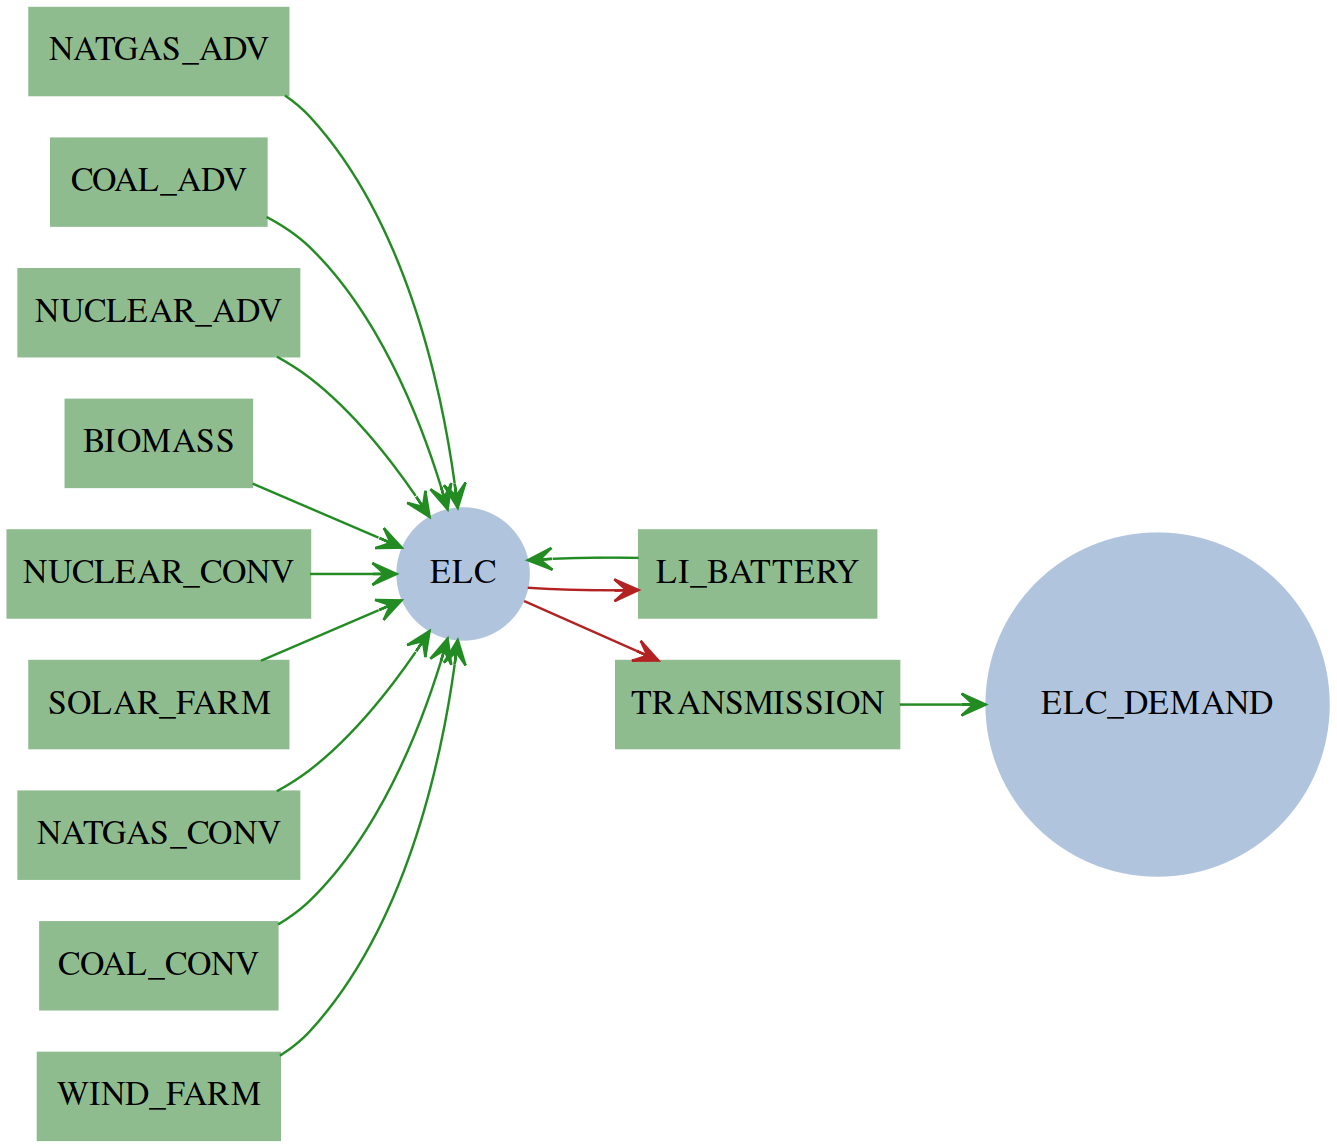
\includegraphics[width=0.6\columnwidth]{IL_system.png}
  \caption{The Illinois electricity grid modeled in \gls{temoa}.}
  \label{fig:ilsys}
\end{figure}

Figure \ref{fig:ilsys} shows the model topology of the Illinois system. There
are nine different electricity generating technologies and one storage option.
All generated electricity passes through a \texttt{TRANSMISSION} technology
to simulate electricity delivery. The Illinois model is spatially and topologically
simple since there are only ten distinct technologies, one region, and one
end-use commodity.

The demand curve for the \texttt{ELC\_DEMAND} commodity is modeled with hourly load
data from the PJM Interconnection. Figure \ref{fig:pjm-elc} shows the historical
electricity demand for PJM and the associated load curve. These data inform the
distribution of annual demand in the \gls{temoa} model, which is scaled by the
total annual demand.

\begin{figure}[H]
  \centering
  \resizebox{\columnwidth}{!}{%% Creator: Matplotlib, PGF backend
%%
%% To include the figure in your LaTeX document, write
%%   \input{<filename>.pgf}
%%
%% Make sure the required packages are loaded in your preamble
%%   \usepackage{pgf}
%%
%% Figures using additional raster images can only be included by \input if
%% they are in the same directory as the main LaTeX file. For loading figures
%% from other directories you can use the `import` package
%%   \usepackage{import}
%%
%% and then include the figures with
%%   \import{<path to file>}{<filename>.pgf}
%%
%% Matplotlib used the following preamble
%%
\begingroup%
\makeatletter%
\begin{pgfpicture}%
\pgfpathrectangle{\pgfpointorigin}{\pgfqpoint{14.900000in}{8.900000in}}%
\pgfusepath{use as bounding box, clip}%
\begin{pgfscope}%
\pgfsetbuttcap%
\pgfsetmiterjoin%
\definecolor{currentfill}{rgb}{1.000000,1.000000,1.000000}%
\pgfsetfillcolor{currentfill}%
\pgfsetlinewidth{0.000000pt}%
\definecolor{currentstroke}{rgb}{0.000000,0.000000,0.000000}%
\pgfsetstrokecolor{currentstroke}%
\pgfsetdash{}{0pt}%
\pgfpathmoveto{\pgfqpoint{0.000000in}{0.000000in}}%
\pgfpathlineto{\pgfqpoint{14.900000in}{0.000000in}}%
\pgfpathlineto{\pgfqpoint{14.900000in}{8.900000in}}%
\pgfpathlineto{\pgfqpoint{0.000000in}{8.900000in}}%
\pgfpathclose%
\pgfusepath{fill}%
\end{pgfscope}%
\begin{pgfscope}%
\pgfsetbuttcap%
\pgfsetmiterjoin%
\definecolor{currentfill}{rgb}{0.827451,0.827451,0.827451}%
\pgfsetfillcolor{currentfill}%
\pgfsetlinewidth{0.000000pt}%
\definecolor{currentstroke}{rgb}{0.000000,0.000000,0.000000}%
\pgfsetstrokecolor{currentstroke}%
\pgfsetstrokeopacity{0.000000}%
\pgfsetdash{}{0pt}%
\pgfpathmoveto{\pgfqpoint{1.079853in}{0.670138in}}%
\pgfpathlineto{\pgfqpoint{10.632936in}{0.670138in}}%
\pgfpathlineto{\pgfqpoint{10.632936in}{8.516628in}}%
\pgfpathlineto{\pgfqpoint{1.079853in}{8.516628in}}%
\pgfpathclose%
\pgfusepath{fill}%
\end{pgfscope}%
\begin{pgfscope}%
\pgfpathrectangle{\pgfqpoint{1.079853in}{0.670138in}}{\pgfqpoint{9.553083in}{7.846490in}}%
\pgfusepath{clip}%
\pgfsetrectcap%
\pgfsetroundjoin%
\pgfsetlinewidth{0.803000pt}%
\definecolor{currentstroke}{rgb}{1.000000,1.000000,1.000000}%
\pgfsetstrokecolor{currentstroke}%
\pgfsetdash{}{0pt}%
\pgfpathmoveto{\pgfqpoint{1.513913in}{0.670138in}}%
\pgfpathlineto{\pgfqpoint{1.513913in}{8.516628in}}%
\pgfusepath{stroke}%
\end{pgfscope}%
\begin{pgfscope}%
\pgfsetbuttcap%
\pgfsetroundjoin%
\definecolor{currentfill}{rgb}{0.000000,0.000000,0.000000}%
\pgfsetfillcolor{currentfill}%
\pgfsetlinewidth{0.803000pt}%
\definecolor{currentstroke}{rgb}{0.000000,0.000000,0.000000}%
\pgfsetstrokecolor{currentstroke}%
\pgfsetdash{}{0pt}%
\pgfsys@defobject{currentmarker}{\pgfqpoint{0.000000in}{-0.048611in}}{\pgfqpoint{0.000000in}{0.000000in}}{%
\pgfpathmoveto{\pgfqpoint{0.000000in}{0.000000in}}%
\pgfpathlineto{\pgfqpoint{0.000000in}{-0.048611in}}%
\pgfusepath{stroke,fill}%
}%
\begin{pgfscope}%
\pgfsys@transformshift{1.513913in}{0.670138in}%
\pgfsys@useobject{currentmarker}{}%
\end{pgfscope}%
\end{pgfscope}%
\begin{pgfscope}%
\definecolor{textcolor}{rgb}{0.000000,0.000000,0.000000}%
\pgfsetstrokecolor{textcolor}%
\pgfsetfillcolor{textcolor}%
\pgftext[x=1.513913in,y=0.572916in,right,top]{\color{textcolor}\rmfamily\fontsize{14.000000}{16.800000}\selectfont \(\displaystyle {2016}\)}%
\end{pgfscope}%
\begin{pgfscope}%
\pgfpathrectangle{\pgfqpoint{1.079853in}{0.670138in}}{\pgfqpoint{9.553083in}{7.846490in}}%
\pgfusepath{clip}%
\pgfsetrectcap%
\pgfsetroundjoin%
\pgfsetlinewidth{0.803000pt}%
\definecolor{currentstroke}{rgb}{1.000000,1.000000,1.000000}%
\pgfsetstrokecolor{currentstroke}%
\pgfsetdash{}{0pt}%
\pgfpathmoveto{\pgfqpoint{3.018236in}{0.670138in}}%
\pgfpathlineto{\pgfqpoint{3.018236in}{8.516628in}}%
\pgfusepath{stroke}%
\end{pgfscope}%
\begin{pgfscope}%
\pgfsetbuttcap%
\pgfsetroundjoin%
\definecolor{currentfill}{rgb}{0.000000,0.000000,0.000000}%
\pgfsetfillcolor{currentfill}%
\pgfsetlinewidth{0.803000pt}%
\definecolor{currentstroke}{rgb}{0.000000,0.000000,0.000000}%
\pgfsetstrokecolor{currentstroke}%
\pgfsetdash{}{0pt}%
\pgfsys@defobject{currentmarker}{\pgfqpoint{0.000000in}{-0.048611in}}{\pgfqpoint{0.000000in}{0.000000in}}{%
\pgfpathmoveto{\pgfqpoint{0.000000in}{0.000000in}}%
\pgfpathlineto{\pgfqpoint{0.000000in}{-0.048611in}}%
\pgfusepath{stroke,fill}%
}%
\begin{pgfscope}%
\pgfsys@transformshift{3.018236in}{0.670138in}%
\pgfsys@useobject{currentmarker}{}%
\end{pgfscope}%
\end{pgfscope}%
\begin{pgfscope}%
\definecolor{textcolor}{rgb}{0.000000,0.000000,0.000000}%
\pgfsetstrokecolor{textcolor}%
\pgfsetfillcolor{textcolor}%
\pgftext[x=3.018236in,y=0.572916in,right,top]{\color{textcolor}\rmfamily\fontsize{14.000000}{16.800000}\selectfont \(\displaystyle {2017}\)}%
\end{pgfscope}%
\begin{pgfscope}%
\pgfpathrectangle{\pgfqpoint{1.079853in}{0.670138in}}{\pgfqpoint{9.553083in}{7.846490in}}%
\pgfusepath{clip}%
\pgfsetrectcap%
\pgfsetroundjoin%
\pgfsetlinewidth{0.803000pt}%
\definecolor{currentstroke}{rgb}{1.000000,1.000000,1.000000}%
\pgfsetstrokecolor{currentstroke}%
\pgfsetdash{}{0pt}%
\pgfpathmoveto{\pgfqpoint{4.518448in}{0.670138in}}%
\pgfpathlineto{\pgfqpoint{4.518448in}{8.516628in}}%
\pgfusepath{stroke}%
\end{pgfscope}%
\begin{pgfscope}%
\pgfsetbuttcap%
\pgfsetroundjoin%
\definecolor{currentfill}{rgb}{0.000000,0.000000,0.000000}%
\pgfsetfillcolor{currentfill}%
\pgfsetlinewidth{0.803000pt}%
\definecolor{currentstroke}{rgb}{0.000000,0.000000,0.000000}%
\pgfsetstrokecolor{currentstroke}%
\pgfsetdash{}{0pt}%
\pgfsys@defobject{currentmarker}{\pgfqpoint{0.000000in}{-0.048611in}}{\pgfqpoint{0.000000in}{0.000000in}}{%
\pgfpathmoveto{\pgfqpoint{0.000000in}{0.000000in}}%
\pgfpathlineto{\pgfqpoint{0.000000in}{-0.048611in}}%
\pgfusepath{stroke,fill}%
}%
\begin{pgfscope}%
\pgfsys@transformshift{4.518448in}{0.670138in}%
\pgfsys@useobject{currentmarker}{}%
\end{pgfscope}%
\end{pgfscope}%
\begin{pgfscope}%
\definecolor{textcolor}{rgb}{0.000000,0.000000,0.000000}%
\pgfsetstrokecolor{textcolor}%
\pgfsetfillcolor{textcolor}%
\pgftext[x=4.518448in,y=0.572916in,right,top]{\color{textcolor}\rmfamily\fontsize{14.000000}{16.800000}\selectfont \(\displaystyle {2018}\)}%
\end{pgfscope}%
\begin{pgfscope}%
\pgfpathrectangle{\pgfqpoint{1.079853in}{0.670138in}}{\pgfqpoint{9.553083in}{7.846490in}}%
\pgfusepath{clip}%
\pgfsetrectcap%
\pgfsetroundjoin%
\pgfsetlinewidth{0.803000pt}%
\definecolor{currentstroke}{rgb}{1.000000,1.000000,1.000000}%
\pgfsetstrokecolor{currentstroke}%
\pgfsetdash{}{0pt}%
\pgfpathmoveto{\pgfqpoint{6.018661in}{0.670138in}}%
\pgfpathlineto{\pgfqpoint{6.018661in}{8.516628in}}%
\pgfusepath{stroke}%
\end{pgfscope}%
\begin{pgfscope}%
\pgfsetbuttcap%
\pgfsetroundjoin%
\definecolor{currentfill}{rgb}{0.000000,0.000000,0.000000}%
\pgfsetfillcolor{currentfill}%
\pgfsetlinewidth{0.803000pt}%
\definecolor{currentstroke}{rgb}{0.000000,0.000000,0.000000}%
\pgfsetstrokecolor{currentstroke}%
\pgfsetdash{}{0pt}%
\pgfsys@defobject{currentmarker}{\pgfqpoint{0.000000in}{-0.048611in}}{\pgfqpoint{0.000000in}{0.000000in}}{%
\pgfpathmoveto{\pgfqpoint{0.000000in}{0.000000in}}%
\pgfpathlineto{\pgfqpoint{0.000000in}{-0.048611in}}%
\pgfusepath{stroke,fill}%
}%
\begin{pgfscope}%
\pgfsys@transformshift{6.018661in}{0.670138in}%
\pgfsys@useobject{currentmarker}{}%
\end{pgfscope}%
\end{pgfscope}%
\begin{pgfscope}%
\definecolor{textcolor}{rgb}{0.000000,0.000000,0.000000}%
\pgfsetstrokecolor{textcolor}%
\pgfsetfillcolor{textcolor}%
\pgftext[x=6.018661in,y=0.572916in,right,top]{\color{textcolor}\rmfamily\fontsize{14.000000}{16.800000}\selectfont \(\displaystyle {2019}\)}%
\end{pgfscope}%
\begin{pgfscope}%
\pgfpathrectangle{\pgfqpoint{1.079853in}{0.670138in}}{\pgfqpoint{9.553083in}{7.846490in}}%
\pgfusepath{clip}%
\pgfsetrectcap%
\pgfsetroundjoin%
\pgfsetlinewidth{0.803000pt}%
\definecolor{currentstroke}{rgb}{1.000000,1.000000,1.000000}%
\pgfsetstrokecolor{currentstroke}%
\pgfsetdash{}{0pt}%
\pgfpathmoveto{\pgfqpoint{7.518873in}{0.670138in}}%
\pgfpathlineto{\pgfqpoint{7.518873in}{8.516628in}}%
\pgfusepath{stroke}%
\end{pgfscope}%
\begin{pgfscope}%
\pgfsetbuttcap%
\pgfsetroundjoin%
\definecolor{currentfill}{rgb}{0.000000,0.000000,0.000000}%
\pgfsetfillcolor{currentfill}%
\pgfsetlinewidth{0.803000pt}%
\definecolor{currentstroke}{rgb}{0.000000,0.000000,0.000000}%
\pgfsetstrokecolor{currentstroke}%
\pgfsetdash{}{0pt}%
\pgfsys@defobject{currentmarker}{\pgfqpoint{0.000000in}{-0.048611in}}{\pgfqpoint{0.000000in}{0.000000in}}{%
\pgfpathmoveto{\pgfqpoint{0.000000in}{0.000000in}}%
\pgfpathlineto{\pgfqpoint{0.000000in}{-0.048611in}}%
\pgfusepath{stroke,fill}%
}%
\begin{pgfscope}%
\pgfsys@transformshift{7.518873in}{0.670138in}%
\pgfsys@useobject{currentmarker}{}%
\end{pgfscope}%
\end{pgfscope}%
\begin{pgfscope}%
\definecolor{textcolor}{rgb}{0.000000,0.000000,0.000000}%
\pgfsetstrokecolor{textcolor}%
\pgfsetfillcolor{textcolor}%
\pgftext[x=7.518873in,y=0.572916in,right,top]{\color{textcolor}\rmfamily\fontsize{14.000000}{16.800000}\selectfont \(\displaystyle {2020}\)}%
\end{pgfscope}%
\begin{pgfscope}%
\pgfpathrectangle{\pgfqpoint{1.079853in}{0.670138in}}{\pgfqpoint{9.553083in}{7.846490in}}%
\pgfusepath{clip}%
\pgfsetrectcap%
\pgfsetroundjoin%
\pgfsetlinewidth{0.803000pt}%
\definecolor{currentstroke}{rgb}{1.000000,1.000000,1.000000}%
\pgfsetstrokecolor{currentstroke}%
\pgfsetdash{}{0pt}%
\pgfpathmoveto{\pgfqpoint{9.023196in}{0.670138in}}%
\pgfpathlineto{\pgfqpoint{9.023196in}{8.516628in}}%
\pgfusepath{stroke}%
\end{pgfscope}%
\begin{pgfscope}%
\pgfsetbuttcap%
\pgfsetroundjoin%
\definecolor{currentfill}{rgb}{0.000000,0.000000,0.000000}%
\pgfsetfillcolor{currentfill}%
\pgfsetlinewidth{0.803000pt}%
\definecolor{currentstroke}{rgb}{0.000000,0.000000,0.000000}%
\pgfsetstrokecolor{currentstroke}%
\pgfsetdash{}{0pt}%
\pgfsys@defobject{currentmarker}{\pgfqpoint{0.000000in}{-0.048611in}}{\pgfqpoint{0.000000in}{0.000000in}}{%
\pgfpathmoveto{\pgfqpoint{0.000000in}{0.000000in}}%
\pgfpathlineto{\pgfqpoint{0.000000in}{-0.048611in}}%
\pgfusepath{stroke,fill}%
}%
\begin{pgfscope}%
\pgfsys@transformshift{9.023196in}{0.670138in}%
\pgfsys@useobject{currentmarker}{}%
\end{pgfscope}%
\end{pgfscope}%
\begin{pgfscope}%
\definecolor{textcolor}{rgb}{0.000000,0.000000,0.000000}%
\pgfsetstrokecolor{textcolor}%
\pgfsetfillcolor{textcolor}%
\pgftext[x=9.023196in,y=0.572916in,right,top]{\color{textcolor}\rmfamily\fontsize{14.000000}{16.800000}\selectfont \(\displaystyle {2021}\)}%
\end{pgfscope}%
\begin{pgfscope}%
\pgfpathrectangle{\pgfqpoint{1.079853in}{0.670138in}}{\pgfqpoint{9.553083in}{7.846490in}}%
\pgfusepath{clip}%
\pgfsetrectcap%
\pgfsetroundjoin%
\pgfsetlinewidth{0.803000pt}%
\definecolor{currentstroke}{rgb}{1.000000,1.000000,1.000000}%
\pgfsetstrokecolor{currentstroke}%
\pgfsetdash{}{0pt}%
\pgfpathmoveto{\pgfqpoint{10.523409in}{0.670138in}}%
\pgfpathlineto{\pgfqpoint{10.523409in}{8.516628in}}%
\pgfusepath{stroke}%
\end{pgfscope}%
\begin{pgfscope}%
\pgfsetbuttcap%
\pgfsetroundjoin%
\definecolor{currentfill}{rgb}{0.000000,0.000000,0.000000}%
\pgfsetfillcolor{currentfill}%
\pgfsetlinewidth{0.803000pt}%
\definecolor{currentstroke}{rgb}{0.000000,0.000000,0.000000}%
\pgfsetstrokecolor{currentstroke}%
\pgfsetdash{}{0pt}%
\pgfsys@defobject{currentmarker}{\pgfqpoint{0.000000in}{-0.048611in}}{\pgfqpoint{0.000000in}{0.000000in}}{%
\pgfpathmoveto{\pgfqpoint{0.000000in}{0.000000in}}%
\pgfpathlineto{\pgfqpoint{0.000000in}{-0.048611in}}%
\pgfusepath{stroke,fill}%
}%
\begin{pgfscope}%
\pgfsys@transformshift{10.523409in}{0.670138in}%
\pgfsys@useobject{currentmarker}{}%
\end{pgfscope}%
\end{pgfscope}%
\begin{pgfscope}%
\definecolor{textcolor}{rgb}{0.000000,0.000000,0.000000}%
\pgfsetstrokecolor{textcolor}%
\pgfsetfillcolor{textcolor}%
\pgftext[x=10.523409in,y=0.572916in,right,top]{\color{textcolor}\rmfamily\fontsize{14.000000}{16.800000}\selectfont \(\displaystyle {2022}\)}%
\end{pgfscope}%
\begin{pgfscope}%
\pgfsetbuttcap%
\pgfsetroundjoin%
\definecolor{currentfill}{rgb}{0.000000,0.000000,0.000000}%
\pgfsetfillcolor{currentfill}%
\pgfsetlinewidth{0.602250pt}%
\definecolor{currentstroke}{rgb}{0.000000,0.000000,0.000000}%
\pgfsetstrokecolor{currentstroke}%
\pgfsetdash{}{0pt}%
\pgfsys@defobject{currentmarker}{\pgfqpoint{0.000000in}{-0.027778in}}{\pgfqpoint{0.000000in}{0.000000in}}{%
\pgfpathmoveto{\pgfqpoint{0.000000in}{0.000000in}}%
\pgfpathlineto{\pgfqpoint{0.000000in}{-0.027778in}}%
\pgfusepath{stroke,fill}%
}%
\begin{pgfscope}%
\pgfsys@transformshift{1.138860in}{0.670138in}%
\pgfsys@useobject{currentmarker}{}%
\end{pgfscope}%
\end{pgfscope}%
\begin{pgfscope}%
\pgfsetbuttcap%
\pgfsetroundjoin%
\definecolor{currentfill}{rgb}{0.000000,0.000000,0.000000}%
\pgfsetfillcolor{currentfill}%
\pgfsetlinewidth{0.602250pt}%
\definecolor{currentstroke}{rgb}{0.000000,0.000000,0.000000}%
\pgfsetstrokecolor{currentstroke}%
\pgfsetdash{}{0pt}%
\pgfsys@defobject{currentmarker}{\pgfqpoint{0.000000in}{-0.027778in}}{\pgfqpoint{0.000000in}{0.000000in}}{%
\pgfpathmoveto{\pgfqpoint{0.000000in}{0.000000in}}%
\pgfpathlineto{\pgfqpoint{0.000000in}{-0.027778in}}%
\pgfusepath{stroke,fill}%
}%
\begin{pgfscope}%
\pgfsys@transformshift{1.888966in}{0.670138in}%
\pgfsys@useobject{currentmarker}{}%
\end{pgfscope}%
\end{pgfscope}%
\begin{pgfscope}%
\pgfsetbuttcap%
\pgfsetroundjoin%
\definecolor{currentfill}{rgb}{0.000000,0.000000,0.000000}%
\pgfsetfillcolor{currentfill}%
\pgfsetlinewidth{0.602250pt}%
\definecolor{currentstroke}{rgb}{0.000000,0.000000,0.000000}%
\pgfsetstrokecolor{currentstroke}%
\pgfsetdash{}{0pt}%
\pgfsys@defobject{currentmarker}{\pgfqpoint{0.000000in}{-0.027778in}}{\pgfqpoint{0.000000in}{0.000000in}}{%
\pgfpathmoveto{\pgfqpoint{0.000000in}{0.000000in}}%
\pgfpathlineto{\pgfqpoint{0.000000in}{-0.027778in}}%
\pgfusepath{stroke,fill}%
}%
\begin{pgfscope}%
\pgfsys@transformshift{2.264019in}{0.670138in}%
\pgfsys@useobject{currentmarker}{}%
\end{pgfscope}%
\end{pgfscope}%
\begin{pgfscope}%
\pgfsetbuttcap%
\pgfsetroundjoin%
\definecolor{currentfill}{rgb}{0.000000,0.000000,0.000000}%
\pgfsetfillcolor{currentfill}%
\pgfsetlinewidth{0.602250pt}%
\definecolor{currentstroke}{rgb}{0.000000,0.000000,0.000000}%
\pgfsetstrokecolor{currentstroke}%
\pgfsetdash{}{0pt}%
\pgfsys@defobject{currentmarker}{\pgfqpoint{0.000000in}{-0.027778in}}{\pgfqpoint{0.000000in}{0.000000in}}{%
\pgfpathmoveto{\pgfqpoint{0.000000in}{0.000000in}}%
\pgfpathlineto{\pgfqpoint{0.000000in}{-0.027778in}}%
\pgfusepath{stroke,fill}%
}%
\begin{pgfscope}%
\pgfsys@transformshift{2.639072in}{0.670138in}%
\pgfsys@useobject{currentmarker}{}%
\end{pgfscope}%
\end{pgfscope}%
\begin{pgfscope}%
\pgfsetbuttcap%
\pgfsetroundjoin%
\definecolor{currentfill}{rgb}{0.000000,0.000000,0.000000}%
\pgfsetfillcolor{currentfill}%
\pgfsetlinewidth{0.602250pt}%
\definecolor{currentstroke}{rgb}{0.000000,0.000000,0.000000}%
\pgfsetstrokecolor{currentstroke}%
\pgfsetdash{}{0pt}%
\pgfsys@defobject{currentmarker}{\pgfqpoint{0.000000in}{-0.027778in}}{\pgfqpoint{0.000000in}{0.000000in}}{%
\pgfpathmoveto{\pgfqpoint{0.000000in}{0.000000in}}%
\pgfpathlineto{\pgfqpoint{0.000000in}{-0.027778in}}%
\pgfusepath{stroke,fill}%
}%
\begin{pgfscope}%
\pgfsys@transformshift{3.014126in}{0.670138in}%
\pgfsys@useobject{currentmarker}{}%
\end{pgfscope}%
\end{pgfscope}%
\begin{pgfscope}%
\pgfsetbuttcap%
\pgfsetroundjoin%
\definecolor{currentfill}{rgb}{0.000000,0.000000,0.000000}%
\pgfsetfillcolor{currentfill}%
\pgfsetlinewidth{0.602250pt}%
\definecolor{currentstroke}{rgb}{0.000000,0.000000,0.000000}%
\pgfsetstrokecolor{currentstroke}%
\pgfsetdash{}{0pt}%
\pgfsys@defobject{currentmarker}{\pgfqpoint{0.000000in}{-0.027778in}}{\pgfqpoint{0.000000in}{0.000000in}}{%
\pgfpathmoveto{\pgfqpoint{0.000000in}{0.000000in}}%
\pgfpathlineto{\pgfqpoint{0.000000in}{-0.027778in}}%
\pgfusepath{stroke,fill}%
}%
\begin{pgfscope}%
\pgfsys@transformshift{3.389179in}{0.670138in}%
\pgfsys@useobject{currentmarker}{}%
\end{pgfscope}%
\end{pgfscope}%
\begin{pgfscope}%
\pgfsetbuttcap%
\pgfsetroundjoin%
\definecolor{currentfill}{rgb}{0.000000,0.000000,0.000000}%
\pgfsetfillcolor{currentfill}%
\pgfsetlinewidth{0.602250pt}%
\definecolor{currentstroke}{rgb}{0.000000,0.000000,0.000000}%
\pgfsetstrokecolor{currentstroke}%
\pgfsetdash{}{0pt}%
\pgfsys@defobject{currentmarker}{\pgfqpoint{0.000000in}{-0.027778in}}{\pgfqpoint{0.000000in}{0.000000in}}{%
\pgfpathmoveto{\pgfqpoint{0.000000in}{0.000000in}}%
\pgfpathlineto{\pgfqpoint{0.000000in}{-0.027778in}}%
\pgfusepath{stroke,fill}%
}%
\begin{pgfscope}%
\pgfsys@transformshift{3.764232in}{0.670138in}%
\pgfsys@useobject{currentmarker}{}%
\end{pgfscope}%
\end{pgfscope}%
\begin{pgfscope}%
\pgfsetbuttcap%
\pgfsetroundjoin%
\definecolor{currentfill}{rgb}{0.000000,0.000000,0.000000}%
\pgfsetfillcolor{currentfill}%
\pgfsetlinewidth{0.602250pt}%
\definecolor{currentstroke}{rgb}{0.000000,0.000000,0.000000}%
\pgfsetstrokecolor{currentstroke}%
\pgfsetdash{}{0pt}%
\pgfsys@defobject{currentmarker}{\pgfqpoint{0.000000in}{-0.027778in}}{\pgfqpoint{0.000000in}{0.000000in}}{%
\pgfpathmoveto{\pgfqpoint{0.000000in}{0.000000in}}%
\pgfpathlineto{\pgfqpoint{0.000000in}{-0.027778in}}%
\pgfusepath{stroke,fill}%
}%
\begin{pgfscope}%
\pgfsys@transformshift{4.139285in}{0.670138in}%
\pgfsys@useobject{currentmarker}{}%
\end{pgfscope}%
\end{pgfscope}%
\begin{pgfscope}%
\pgfsetbuttcap%
\pgfsetroundjoin%
\definecolor{currentfill}{rgb}{0.000000,0.000000,0.000000}%
\pgfsetfillcolor{currentfill}%
\pgfsetlinewidth{0.602250pt}%
\definecolor{currentstroke}{rgb}{0.000000,0.000000,0.000000}%
\pgfsetstrokecolor{currentstroke}%
\pgfsetdash{}{0pt}%
\pgfsys@defobject{currentmarker}{\pgfqpoint{0.000000in}{-0.027778in}}{\pgfqpoint{0.000000in}{0.000000in}}{%
\pgfpathmoveto{\pgfqpoint{0.000000in}{0.000000in}}%
\pgfpathlineto{\pgfqpoint{0.000000in}{-0.027778in}}%
\pgfusepath{stroke,fill}%
}%
\begin{pgfscope}%
\pgfsys@transformshift{4.514338in}{0.670138in}%
\pgfsys@useobject{currentmarker}{}%
\end{pgfscope}%
\end{pgfscope}%
\begin{pgfscope}%
\pgfsetbuttcap%
\pgfsetroundjoin%
\definecolor{currentfill}{rgb}{0.000000,0.000000,0.000000}%
\pgfsetfillcolor{currentfill}%
\pgfsetlinewidth{0.602250pt}%
\definecolor{currentstroke}{rgb}{0.000000,0.000000,0.000000}%
\pgfsetstrokecolor{currentstroke}%
\pgfsetdash{}{0pt}%
\pgfsys@defobject{currentmarker}{\pgfqpoint{0.000000in}{-0.027778in}}{\pgfqpoint{0.000000in}{0.000000in}}{%
\pgfpathmoveto{\pgfqpoint{0.000000in}{0.000000in}}%
\pgfpathlineto{\pgfqpoint{0.000000in}{-0.027778in}}%
\pgfusepath{stroke,fill}%
}%
\begin{pgfscope}%
\pgfsys@transformshift{4.889391in}{0.670138in}%
\pgfsys@useobject{currentmarker}{}%
\end{pgfscope}%
\end{pgfscope}%
\begin{pgfscope}%
\pgfsetbuttcap%
\pgfsetroundjoin%
\definecolor{currentfill}{rgb}{0.000000,0.000000,0.000000}%
\pgfsetfillcolor{currentfill}%
\pgfsetlinewidth{0.602250pt}%
\definecolor{currentstroke}{rgb}{0.000000,0.000000,0.000000}%
\pgfsetstrokecolor{currentstroke}%
\pgfsetdash{}{0pt}%
\pgfsys@defobject{currentmarker}{\pgfqpoint{0.000000in}{-0.027778in}}{\pgfqpoint{0.000000in}{0.000000in}}{%
\pgfpathmoveto{\pgfqpoint{0.000000in}{0.000000in}}%
\pgfpathlineto{\pgfqpoint{0.000000in}{-0.027778in}}%
\pgfusepath{stroke,fill}%
}%
\begin{pgfscope}%
\pgfsys@transformshift{5.264444in}{0.670138in}%
\pgfsys@useobject{currentmarker}{}%
\end{pgfscope}%
\end{pgfscope}%
\begin{pgfscope}%
\pgfsetbuttcap%
\pgfsetroundjoin%
\definecolor{currentfill}{rgb}{0.000000,0.000000,0.000000}%
\pgfsetfillcolor{currentfill}%
\pgfsetlinewidth{0.602250pt}%
\definecolor{currentstroke}{rgb}{0.000000,0.000000,0.000000}%
\pgfsetstrokecolor{currentstroke}%
\pgfsetdash{}{0pt}%
\pgfsys@defobject{currentmarker}{\pgfqpoint{0.000000in}{-0.027778in}}{\pgfqpoint{0.000000in}{0.000000in}}{%
\pgfpathmoveto{\pgfqpoint{0.000000in}{0.000000in}}%
\pgfpathlineto{\pgfqpoint{0.000000in}{-0.027778in}}%
\pgfusepath{stroke,fill}%
}%
\begin{pgfscope}%
\pgfsys@transformshift{5.639498in}{0.670138in}%
\pgfsys@useobject{currentmarker}{}%
\end{pgfscope}%
\end{pgfscope}%
\begin{pgfscope}%
\pgfsetbuttcap%
\pgfsetroundjoin%
\definecolor{currentfill}{rgb}{0.000000,0.000000,0.000000}%
\pgfsetfillcolor{currentfill}%
\pgfsetlinewidth{0.602250pt}%
\definecolor{currentstroke}{rgb}{0.000000,0.000000,0.000000}%
\pgfsetstrokecolor{currentstroke}%
\pgfsetdash{}{0pt}%
\pgfsys@defobject{currentmarker}{\pgfqpoint{0.000000in}{-0.027778in}}{\pgfqpoint{0.000000in}{0.000000in}}{%
\pgfpathmoveto{\pgfqpoint{0.000000in}{0.000000in}}%
\pgfpathlineto{\pgfqpoint{0.000000in}{-0.027778in}}%
\pgfusepath{stroke,fill}%
}%
\begin{pgfscope}%
\pgfsys@transformshift{6.014551in}{0.670138in}%
\pgfsys@useobject{currentmarker}{}%
\end{pgfscope}%
\end{pgfscope}%
\begin{pgfscope}%
\pgfsetbuttcap%
\pgfsetroundjoin%
\definecolor{currentfill}{rgb}{0.000000,0.000000,0.000000}%
\pgfsetfillcolor{currentfill}%
\pgfsetlinewidth{0.602250pt}%
\definecolor{currentstroke}{rgb}{0.000000,0.000000,0.000000}%
\pgfsetstrokecolor{currentstroke}%
\pgfsetdash{}{0pt}%
\pgfsys@defobject{currentmarker}{\pgfqpoint{0.000000in}{-0.027778in}}{\pgfqpoint{0.000000in}{0.000000in}}{%
\pgfpathmoveto{\pgfqpoint{0.000000in}{0.000000in}}%
\pgfpathlineto{\pgfqpoint{0.000000in}{-0.027778in}}%
\pgfusepath{stroke,fill}%
}%
\begin{pgfscope}%
\pgfsys@transformshift{6.389604in}{0.670138in}%
\pgfsys@useobject{currentmarker}{}%
\end{pgfscope}%
\end{pgfscope}%
\begin{pgfscope}%
\pgfsetbuttcap%
\pgfsetroundjoin%
\definecolor{currentfill}{rgb}{0.000000,0.000000,0.000000}%
\pgfsetfillcolor{currentfill}%
\pgfsetlinewidth{0.602250pt}%
\definecolor{currentstroke}{rgb}{0.000000,0.000000,0.000000}%
\pgfsetstrokecolor{currentstroke}%
\pgfsetdash{}{0pt}%
\pgfsys@defobject{currentmarker}{\pgfqpoint{0.000000in}{-0.027778in}}{\pgfqpoint{0.000000in}{0.000000in}}{%
\pgfpathmoveto{\pgfqpoint{0.000000in}{0.000000in}}%
\pgfpathlineto{\pgfqpoint{0.000000in}{-0.027778in}}%
\pgfusepath{stroke,fill}%
}%
\begin{pgfscope}%
\pgfsys@transformshift{6.764657in}{0.670138in}%
\pgfsys@useobject{currentmarker}{}%
\end{pgfscope}%
\end{pgfscope}%
\begin{pgfscope}%
\pgfsetbuttcap%
\pgfsetroundjoin%
\definecolor{currentfill}{rgb}{0.000000,0.000000,0.000000}%
\pgfsetfillcolor{currentfill}%
\pgfsetlinewidth{0.602250pt}%
\definecolor{currentstroke}{rgb}{0.000000,0.000000,0.000000}%
\pgfsetstrokecolor{currentstroke}%
\pgfsetdash{}{0pt}%
\pgfsys@defobject{currentmarker}{\pgfqpoint{0.000000in}{-0.027778in}}{\pgfqpoint{0.000000in}{0.000000in}}{%
\pgfpathmoveto{\pgfqpoint{0.000000in}{0.000000in}}%
\pgfpathlineto{\pgfqpoint{0.000000in}{-0.027778in}}%
\pgfusepath{stroke,fill}%
}%
\begin{pgfscope}%
\pgfsys@transformshift{7.139710in}{0.670138in}%
\pgfsys@useobject{currentmarker}{}%
\end{pgfscope}%
\end{pgfscope}%
\begin{pgfscope}%
\pgfsetbuttcap%
\pgfsetroundjoin%
\definecolor{currentfill}{rgb}{0.000000,0.000000,0.000000}%
\pgfsetfillcolor{currentfill}%
\pgfsetlinewidth{0.602250pt}%
\definecolor{currentstroke}{rgb}{0.000000,0.000000,0.000000}%
\pgfsetstrokecolor{currentstroke}%
\pgfsetdash{}{0pt}%
\pgfsys@defobject{currentmarker}{\pgfqpoint{0.000000in}{-0.027778in}}{\pgfqpoint{0.000000in}{0.000000in}}{%
\pgfpathmoveto{\pgfqpoint{0.000000in}{0.000000in}}%
\pgfpathlineto{\pgfqpoint{0.000000in}{-0.027778in}}%
\pgfusepath{stroke,fill}%
}%
\begin{pgfscope}%
\pgfsys@transformshift{7.514763in}{0.670138in}%
\pgfsys@useobject{currentmarker}{}%
\end{pgfscope}%
\end{pgfscope}%
\begin{pgfscope}%
\pgfsetbuttcap%
\pgfsetroundjoin%
\definecolor{currentfill}{rgb}{0.000000,0.000000,0.000000}%
\pgfsetfillcolor{currentfill}%
\pgfsetlinewidth{0.602250pt}%
\definecolor{currentstroke}{rgb}{0.000000,0.000000,0.000000}%
\pgfsetstrokecolor{currentstroke}%
\pgfsetdash{}{0pt}%
\pgfsys@defobject{currentmarker}{\pgfqpoint{0.000000in}{-0.027778in}}{\pgfqpoint{0.000000in}{0.000000in}}{%
\pgfpathmoveto{\pgfqpoint{0.000000in}{0.000000in}}%
\pgfpathlineto{\pgfqpoint{0.000000in}{-0.027778in}}%
\pgfusepath{stroke,fill}%
}%
\begin{pgfscope}%
\pgfsys@transformshift{7.889816in}{0.670138in}%
\pgfsys@useobject{currentmarker}{}%
\end{pgfscope}%
\end{pgfscope}%
\begin{pgfscope}%
\pgfsetbuttcap%
\pgfsetroundjoin%
\definecolor{currentfill}{rgb}{0.000000,0.000000,0.000000}%
\pgfsetfillcolor{currentfill}%
\pgfsetlinewidth{0.602250pt}%
\definecolor{currentstroke}{rgb}{0.000000,0.000000,0.000000}%
\pgfsetstrokecolor{currentstroke}%
\pgfsetdash{}{0pt}%
\pgfsys@defobject{currentmarker}{\pgfqpoint{0.000000in}{-0.027778in}}{\pgfqpoint{0.000000in}{0.000000in}}{%
\pgfpathmoveto{\pgfqpoint{0.000000in}{0.000000in}}%
\pgfpathlineto{\pgfqpoint{0.000000in}{-0.027778in}}%
\pgfusepath{stroke,fill}%
}%
\begin{pgfscope}%
\pgfsys@transformshift{8.264869in}{0.670138in}%
\pgfsys@useobject{currentmarker}{}%
\end{pgfscope}%
\end{pgfscope}%
\begin{pgfscope}%
\pgfsetbuttcap%
\pgfsetroundjoin%
\definecolor{currentfill}{rgb}{0.000000,0.000000,0.000000}%
\pgfsetfillcolor{currentfill}%
\pgfsetlinewidth{0.602250pt}%
\definecolor{currentstroke}{rgb}{0.000000,0.000000,0.000000}%
\pgfsetstrokecolor{currentstroke}%
\pgfsetdash{}{0pt}%
\pgfsys@defobject{currentmarker}{\pgfqpoint{0.000000in}{-0.027778in}}{\pgfqpoint{0.000000in}{0.000000in}}{%
\pgfpathmoveto{\pgfqpoint{0.000000in}{0.000000in}}%
\pgfpathlineto{\pgfqpoint{0.000000in}{-0.027778in}}%
\pgfusepath{stroke,fill}%
}%
\begin{pgfscope}%
\pgfsys@transformshift{8.639923in}{0.670138in}%
\pgfsys@useobject{currentmarker}{}%
\end{pgfscope}%
\end{pgfscope}%
\begin{pgfscope}%
\pgfsetbuttcap%
\pgfsetroundjoin%
\definecolor{currentfill}{rgb}{0.000000,0.000000,0.000000}%
\pgfsetfillcolor{currentfill}%
\pgfsetlinewidth{0.602250pt}%
\definecolor{currentstroke}{rgb}{0.000000,0.000000,0.000000}%
\pgfsetstrokecolor{currentstroke}%
\pgfsetdash{}{0pt}%
\pgfsys@defobject{currentmarker}{\pgfqpoint{0.000000in}{-0.027778in}}{\pgfqpoint{0.000000in}{0.000000in}}{%
\pgfpathmoveto{\pgfqpoint{0.000000in}{0.000000in}}%
\pgfpathlineto{\pgfqpoint{0.000000in}{-0.027778in}}%
\pgfusepath{stroke,fill}%
}%
\begin{pgfscope}%
\pgfsys@transformshift{9.014976in}{0.670138in}%
\pgfsys@useobject{currentmarker}{}%
\end{pgfscope}%
\end{pgfscope}%
\begin{pgfscope}%
\pgfsetbuttcap%
\pgfsetroundjoin%
\definecolor{currentfill}{rgb}{0.000000,0.000000,0.000000}%
\pgfsetfillcolor{currentfill}%
\pgfsetlinewidth{0.602250pt}%
\definecolor{currentstroke}{rgb}{0.000000,0.000000,0.000000}%
\pgfsetstrokecolor{currentstroke}%
\pgfsetdash{}{0pt}%
\pgfsys@defobject{currentmarker}{\pgfqpoint{0.000000in}{-0.027778in}}{\pgfqpoint{0.000000in}{0.000000in}}{%
\pgfpathmoveto{\pgfqpoint{0.000000in}{0.000000in}}%
\pgfpathlineto{\pgfqpoint{0.000000in}{-0.027778in}}%
\pgfusepath{stroke,fill}%
}%
\begin{pgfscope}%
\pgfsys@transformshift{9.390029in}{0.670138in}%
\pgfsys@useobject{currentmarker}{}%
\end{pgfscope}%
\end{pgfscope}%
\begin{pgfscope}%
\pgfsetbuttcap%
\pgfsetroundjoin%
\definecolor{currentfill}{rgb}{0.000000,0.000000,0.000000}%
\pgfsetfillcolor{currentfill}%
\pgfsetlinewidth{0.602250pt}%
\definecolor{currentstroke}{rgb}{0.000000,0.000000,0.000000}%
\pgfsetstrokecolor{currentstroke}%
\pgfsetdash{}{0pt}%
\pgfsys@defobject{currentmarker}{\pgfqpoint{0.000000in}{-0.027778in}}{\pgfqpoint{0.000000in}{0.000000in}}{%
\pgfpathmoveto{\pgfqpoint{0.000000in}{0.000000in}}%
\pgfpathlineto{\pgfqpoint{0.000000in}{-0.027778in}}%
\pgfusepath{stroke,fill}%
}%
\begin{pgfscope}%
\pgfsys@transformshift{9.765082in}{0.670138in}%
\pgfsys@useobject{currentmarker}{}%
\end{pgfscope}%
\end{pgfscope}%
\begin{pgfscope}%
\pgfsetbuttcap%
\pgfsetroundjoin%
\definecolor{currentfill}{rgb}{0.000000,0.000000,0.000000}%
\pgfsetfillcolor{currentfill}%
\pgfsetlinewidth{0.602250pt}%
\definecolor{currentstroke}{rgb}{0.000000,0.000000,0.000000}%
\pgfsetstrokecolor{currentstroke}%
\pgfsetdash{}{0pt}%
\pgfsys@defobject{currentmarker}{\pgfqpoint{0.000000in}{-0.027778in}}{\pgfqpoint{0.000000in}{0.000000in}}{%
\pgfpathmoveto{\pgfqpoint{0.000000in}{0.000000in}}%
\pgfpathlineto{\pgfqpoint{0.000000in}{-0.027778in}}%
\pgfusepath{stroke,fill}%
}%
\begin{pgfscope}%
\pgfsys@transformshift{10.140135in}{0.670138in}%
\pgfsys@useobject{currentmarker}{}%
\end{pgfscope}%
\end{pgfscope}%
\begin{pgfscope}%
\pgfsetbuttcap%
\pgfsetroundjoin%
\definecolor{currentfill}{rgb}{0.000000,0.000000,0.000000}%
\pgfsetfillcolor{currentfill}%
\pgfsetlinewidth{0.602250pt}%
\definecolor{currentstroke}{rgb}{0.000000,0.000000,0.000000}%
\pgfsetstrokecolor{currentstroke}%
\pgfsetdash{}{0pt}%
\pgfsys@defobject{currentmarker}{\pgfqpoint{0.000000in}{-0.027778in}}{\pgfqpoint{0.000000in}{0.000000in}}{%
\pgfpathmoveto{\pgfqpoint{0.000000in}{0.000000in}}%
\pgfpathlineto{\pgfqpoint{0.000000in}{-0.027778in}}%
\pgfusepath{stroke,fill}%
}%
\begin{pgfscope}%
\pgfsys@transformshift{10.515188in}{0.670138in}%
\pgfsys@useobject{currentmarker}{}%
\end{pgfscope}%
\end{pgfscope}%
\begin{pgfscope}%
\definecolor{textcolor}{rgb}{0.000000,0.000000,0.000000}%
\pgfsetstrokecolor{textcolor}%
\pgfsetfillcolor{textcolor}%
\pgftext[x=5.856395in,y=0.339583in,,top]{\color{textcolor}\rmfamily\fontsize{18.000000}{21.600000}\selectfont Time [hours]}%
\end{pgfscope}%
\begin{pgfscope}%
\pgfpathrectangle{\pgfqpoint{1.079853in}{0.670138in}}{\pgfqpoint{9.553083in}{7.846490in}}%
\pgfusepath{clip}%
\pgfsetrectcap%
\pgfsetroundjoin%
\pgfsetlinewidth{0.803000pt}%
\definecolor{currentstroke}{rgb}{1.000000,1.000000,1.000000}%
\pgfsetstrokecolor{currentstroke}%
\pgfsetdash{}{0pt}%
\pgfpathmoveto{\pgfqpoint{1.079853in}{0.800497in}}%
\pgfpathlineto{\pgfqpoint{10.632936in}{0.800497in}}%
\pgfusepath{stroke}%
\end{pgfscope}%
\begin{pgfscope}%
\pgfsetbuttcap%
\pgfsetroundjoin%
\definecolor{currentfill}{rgb}{0.000000,0.000000,0.000000}%
\pgfsetfillcolor{currentfill}%
\pgfsetlinewidth{0.803000pt}%
\definecolor{currentstroke}{rgb}{0.000000,0.000000,0.000000}%
\pgfsetstrokecolor{currentstroke}%
\pgfsetdash{}{0pt}%
\pgfsys@defobject{currentmarker}{\pgfqpoint{-0.048611in}{0.000000in}}{\pgfqpoint{-0.000000in}{0.000000in}}{%
\pgfpathmoveto{\pgfqpoint{-0.000000in}{0.000000in}}%
\pgfpathlineto{\pgfqpoint{-0.048611in}{0.000000in}}%
\pgfusepath{stroke,fill}%
}%
\begin{pgfscope}%
\pgfsys@transformshift{1.079853in}{0.800497in}%
\pgfsys@useobject{currentmarker}{}%
\end{pgfscope}%
\end{pgfscope}%
\begin{pgfscope}%
\definecolor{textcolor}{rgb}{0.000000,0.000000,0.000000}%
\pgfsetstrokecolor{textcolor}%
\pgfsetfillcolor{textcolor}%
\pgftext[x=0.493054in, y=0.731053in, left, base]{\color{textcolor}\rmfamily\fontsize{14.000000}{16.800000}\selectfont \(\displaystyle {60000}\)}%
\end{pgfscope}%
\begin{pgfscope}%
\pgfpathrectangle{\pgfqpoint{1.079853in}{0.670138in}}{\pgfqpoint{9.553083in}{7.846490in}}%
\pgfusepath{clip}%
\pgfsetrectcap%
\pgfsetroundjoin%
\pgfsetlinewidth{0.803000pt}%
\definecolor{currentstroke}{rgb}{1.000000,1.000000,1.000000}%
\pgfsetstrokecolor{currentstroke}%
\pgfsetdash{}{0pt}%
\pgfpathmoveto{\pgfqpoint{1.079853in}{2.515745in}}%
\pgfpathlineto{\pgfqpoint{10.632936in}{2.515745in}}%
\pgfusepath{stroke}%
\end{pgfscope}%
\begin{pgfscope}%
\pgfsetbuttcap%
\pgfsetroundjoin%
\definecolor{currentfill}{rgb}{0.000000,0.000000,0.000000}%
\pgfsetfillcolor{currentfill}%
\pgfsetlinewidth{0.803000pt}%
\definecolor{currentstroke}{rgb}{0.000000,0.000000,0.000000}%
\pgfsetstrokecolor{currentstroke}%
\pgfsetdash{}{0pt}%
\pgfsys@defobject{currentmarker}{\pgfqpoint{-0.048611in}{0.000000in}}{\pgfqpoint{-0.000000in}{0.000000in}}{%
\pgfpathmoveto{\pgfqpoint{-0.000000in}{0.000000in}}%
\pgfpathlineto{\pgfqpoint{-0.048611in}{0.000000in}}%
\pgfusepath{stroke,fill}%
}%
\begin{pgfscope}%
\pgfsys@transformshift{1.079853in}{2.515745in}%
\pgfsys@useobject{currentmarker}{}%
\end{pgfscope}%
\end{pgfscope}%
\begin{pgfscope}%
\definecolor{textcolor}{rgb}{0.000000,0.000000,0.000000}%
\pgfsetstrokecolor{textcolor}%
\pgfsetfillcolor{textcolor}%
\pgftext[x=0.493054in, y=2.446301in, left, base]{\color{textcolor}\rmfamily\fontsize{14.000000}{16.800000}\selectfont \(\displaystyle {80000}\)}%
\end{pgfscope}%
\begin{pgfscope}%
\pgfpathrectangle{\pgfqpoint{1.079853in}{0.670138in}}{\pgfqpoint{9.553083in}{7.846490in}}%
\pgfusepath{clip}%
\pgfsetrectcap%
\pgfsetroundjoin%
\pgfsetlinewidth{0.803000pt}%
\definecolor{currentstroke}{rgb}{1.000000,1.000000,1.000000}%
\pgfsetstrokecolor{currentstroke}%
\pgfsetdash{}{0pt}%
\pgfpathmoveto{\pgfqpoint{1.079853in}{4.230994in}}%
\pgfpathlineto{\pgfqpoint{10.632936in}{4.230994in}}%
\pgfusepath{stroke}%
\end{pgfscope}%
\begin{pgfscope}%
\pgfsetbuttcap%
\pgfsetroundjoin%
\definecolor{currentfill}{rgb}{0.000000,0.000000,0.000000}%
\pgfsetfillcolor{currentfill}%
\pgfsetlinewidth{0.803000pt}%
\definecolor{currentstroke}{rgb}{0.000000,0.000000,0.000000}%
\pgfsetstrokecolor{currentstroke}%
\pgfsetdash{}{0pt}%
\pgfsys@defobject{currentmarker}{\pgfqpoint{-0.048611in}{0.000000in}}{\pgfqpoint{-0.000000in}{0.000000in}}{%
\pgfpathmoveto{\pgfqpoint{-0.000000in}{0.000000in}}%
\pgfpathlineto{\pgfqpoint{-0.048611in}{0.000000in}}%
\pgfusepath{stroke,fill}%
}%
\begin{pgfscope}%
\pgfsys@transformshift{1.079853in}{4.230994in}%
\pgfsys@useobject{currentmarker}{}%
\end{pgfscope}%
\end{pgfscope}%
\begin{pgfscope}%
\definecolor{textcolor}{rgb}{0.000000,0.000000,0.000000}%
\pgfsetstrokecolor{textcolor}%
\pgfsetfillcolor{textcolor}%
\pgftext[x=0.395138in, y=4.161550in, left, base]{\color{textcolor}\rmfamily\fontsize{14.000000}{16.800000}\selectfont \(\displaystyle {100000}\)}%
\end{pgfscope}%
\begin{pgfscope}%
\pgfpathrectangle{\pgfqpoint{1.079853in}{0.670138in}}{\pgfqpoint{9.553083in}{7.846490in}}%
\pgfusepath{clip}%
\pgfsetrectcap%
\pgfsetroundjoin%
\pgfsetlinewidth{0.803000pt}%
\definecolor{currentstroke}{rgb}{1.000000,1.000000,1.000000}%
\pgfsetstrokecolor{currentstroke}%
\pgfsetdash{}{0pt}%
\pgfpathmoveto{\pgfqpoint{1.079853in}{5.946243in}}%
\pgfpathlineto{\pgfqpoint{10.632936in}{5.946243in}}%
\pgfusepath{stroke}%
\end{pgfscope}%
\begin{pgfscope}%
\pgfsetbuttcap%
\pgfsetroundjoin%
\definecolor{currentfill}{rgb}{0.000000,0.000000,0.000000}%
\pgfsetfillcolor{currentfill}%
\pgfsetlinewidth{0.803000pt}%
\definecolor{currentstroke}{rgb}{0.000000,0.000000,0.000000}%
\pgfsetstrokecolor{currentstroke}%
\pgfsetdash{}{0pt}%
\pgfsys@defobject{currentmarker}{\pgfqpoint{-0.048611in}{0.000000in}}{\pgfqpoint{-0.000000in}{0.000000in}}{%
\pgfpathmoveto{\pgfqpoint{-0.000000in}{0.000000in}}%
\pgfpathlineto{\pgfqpoint{-0.048611in}{0.000000in}}%
\pgfusepath{stroke,fill}%
}%
\begin{pgfscope}%
\pgfsys@transformshift{1.079853in}{5.946243in}%
\pgfsys@useobject{currentmarker}{}%
\end{pgfscope}%
\end{pgfscope}%
\begin{pgfscope}%
\definecolor{textcolor}{rgb}{0.000000,0.000000,0.000000}%
\pgfsetstrokecolor{textcolor}%
\pgfsetfillcolor{textcolor}%
\pgftext[x=0.395138in, y=5.876798in, left, base]{\color{textcolor}\rmfamily\fontsize{14.000000}{16.800000}\selectfont \(\displaystyle {120000}\)}%
\end{pgfscope}%
\begin{pgfscope}%
\pgfpathrectangle{\pgfqpoint{1.079853in}{0.670138in}}{\pgfqpoint{9.553083in}{7.846490in}}%
\pgfusepath{clip}%
\pgfsetrectcap%
\pgfsetroundjoin%
\pgfsetlinewidth{0.803000pt}%
\definecolor{currentstroke}{rgb}{1.000000,1.000000,1.000000}%
\pgfsetstrokecolor{currentstroke}%
\pgfsetdash{}{0pt}%
\pgfpathmoveto{\pgfqpoint{1.079853in}{7.661491in}}%
\pgfpathlineto{\pgfqpoint{10.632936in}{7.661491in}}%
\pgfusepath{stroke}%
\end{pgfscope}%
\begin{pgfscope}%
\pgfsetbuttcap%
\pgfsetroundjoin%
\definecolor{currentfill}{rgb}{0.000000,0.000000,0.000000}%
\pgfsetfillcolor{currentfill}%
\pgfsetlinewidth{0.803000pt}%
\definecolor{currentstroke}{rgb}{0.000000,0.000000,0.000000}%
\pgfsetstrokecolor{currentstroke}%
\pgfsetdash{}{0pt}%
\pgfsys@defobject{currentmarker}{\pgfqpoint{-0.048611in}{0.000000in}}{\pgfqpoint{-0.000000in}{0.000000in}}{%
\pgfpathmoveto{\pgfqpoint{-0.000000in}{0.000000in}}%
\pgfpathlineto{\pgfqpoint{-0.048611in}{0.000000in}}%
\pgfusepath{stroke,fill}%
}%
\begin{pgfscope}%
\pgfsys@transformshift{1.079853in}{7.661491in}%
\pgfsys@useobject{currentmarker}{}%
\end{pgfscope}%
\end{pgfscope}%
\begin{pgfscope}%
\definecolor{textcolor}{rgb}{0.000000,0.000000,0.000000}%
\pgfsetstrokecolor{textcolor}%
\pgfsetfillcolor{textcolor}%
\pgftext[x=0.395138in, y=7.592047in, left, base]{\color{textcolor}\rmfamily\fontsize{14.000000}{16.800000}\selectfont \(\displaystyle {140000}\)}%
\end{pgfscope}%
\begin{pgfscope}%
\pgfsetbuttcap%
\pgfsetroundjoin%
\definecolor{currentfill}{rgb}{0.000000,0.000000,0.000000}%
\pgfsetfillcolor{currentfill}%
\pgfsetlinewidth{0.602250pt}%
\definecolor{currentstroke}{rgb}{0.000000,0.000000,0.000000}%
\pgfsetstrokecolor{currentstroke}%
\pgfsetdash{}{0pt}%
\pgfsys@defobject{currentmarker}{\pgfqpoint{-0.027778in}{0.000000in}}{\pgfqpoint{-0.000000in}{0.000000in}}{%
\pgfpathmoveto{\pgfqpoint{-0.000000in}{0.000000in}}%
\pgfpathlineto{\pgfqpoint{-0.027778in}{0.000000in}}%
\pgfusepath{stroke,fill}%
}%
\begin{pgfscope}%
\pgfsys@transformshift{1.079853in}{1.229309in}%
\pgfsys@useobject{currentmarker}{}%
\end{pgfscope}%
\end{pgfscope}%
\begin{pgfscope}%
\pgfsetbuttcap%
\pgfsetroundjoin%
\definecolor{currentfill}{rgb}{0.000000,0.000000,0.000000}%
\pgfsetfillcolor{currentfill}%
\pgfsetlinewidth{0.602250pt}%
\definecolor{currentstroke}{rgb}{0.000000,0.000000,0.000000}%
\pgfsetstrokecolor{currentstroke}%
\pgfsetdash{}{0pt}%
\pgfsys@defobject{currentmarker}{\pgfqpoint{-0.027778in}{0.000000in}}{\pgfqpoint{-0.000000in}{0.000000in}}{%
\pgfpathmoveto{\pgfqpoint{-0.000000in}{0.000000in}}%
\pgfpathlineto{\pgfqpoint{-0.027778in}{0.000000in}}%
\pgfusepath{stroke,fill}%
}%
\begin{pgfscope}%
\pgfsys@transformshift{1.079853in}{1.658121in}%
\pgfsys@useobject{currentmarker}{}%
\end{pgfscope}%
\end{pgfscope}%
\begin{pgfscope}%
\pgfsetbuttcap%
\pgfsetroundjoin%
\definecolor{currentfill}{rgb}{0.000000,0.000000,0.000000}%
\pgfsetfillcolor{currentfill}%
\pgfsetlinewidth{0.602250pt}%
\definecolor{currentstroke}{rgb}{0.000000,0.000000,0.000000}%
\pgfsetstrokecolor{currentstroke}%
\pgfsetdash{}{0pt}%
\pgfsys@defobject{currentmarker}{\pgfqpoint{-0.027778in}{0.000000in}}{\pgfqpoint{-0.000000in}{0.000000in}}{%
\pgfpathmoveto{\pgfqpoint{-0.000000in}{0.000000in}}%
\pgfpathlineto{\pgfqpoint{-0.027778in}{0.000000in}}%
\pgfusepath{stroke,fill}%
}%
\begin{pgfscope}%
\pgfsys@transformshift{1.079853in}{2.086933in}%
\pgfsys@useobject{currentmarker}{}%
\end{pgfscope}%
\end{pgfscope}%
\begin{pgfscope}%
\pgfsetbuttcap%
\pgfsetroundjoin%
\definecolor{currentfill}{rgb}{0.000000,0.000000,0.000000}%
\pgfsetfillcolor{currentfill}%
\pgfsetlinewidth{0.602250pt}%
\definecolor{currentstroke}{rgb}{0.000000,0.000000,0.000000}%
\pgfsetstrokecolor{currentstroke}%
\pgfsetdash{}{0pt}%
\pgfsys@defobject{currentmarker}{\pgfqpoint{-0.027778in}{0.000000in}}{\pgfqpoint{-0.000000in}{0.000000in}}{%
\pgfpathmoveto{\pgfqpoint{-0.000000in}{0.000000in}}%
\pgfpathlineto{\pgfqpoint{-0.027778in}{0.000000in}}%
\pgfusepath{stroke,fill}%
}%
\begin{pgfscope}%
\pgfsys@transformshift{1.079853in}{2.944558in}%
\pgfsys@useobject{currentmarker}{}%
\end{pgfscope}%
\end{pgfscope}%
\begin{pgfscope}%
\pgfsetbuttcap%
\pgfsetroundjoin%
\definecolor{currentfill}{rgb}{0.000000,0.000000,0.000000}%
\pgfsetfillcolor{currentfill}%
\pgfsetlinewidth{0.602250pt}%
\definecolor{currentstroke}{rgb}{0.000000,0.000000,0.000000}%
\pgfsetstrokecolor{currentstroke}%
\pgfsetdash{}{0pt}%
\pgfsys@defobject{currentmarker}{\pgfqpoint{-0.027778in}{0.000000in}}{\pgfqpoint{-0.000000in}{0.000000in}}{%
\pgfpathmoveto{\pgfqpoint{-0.000000in}{0.000000in}}%
\pgfpathlineto{\pgfqpoint{-0.027778in}{0.000000in}}%
\pgfusepath{stroke,fill}%
}%
\begin{pgfscope}%
\pgfsys@transformshift{1.079853in}{3.373370in}%
\pgfsys@useobject{currentmarker}{}%
\end{pgfscope}%
\end{pgfscope}%
\begin{pgfscope}%
\pgfsetbuttcap%
\pgfsetroundjoin%
\definecolor{currentfill}{rgb}{0.000000,0.000000,0.000000}%
\pgfsetfillcolor{currentfill}%
\pgfsetlinewidth{0.602250pt}%
\definecolor{currentstroke}{rgb}{0.000000,0.000000,0.000000}%
\pgfsetstrokecolor{currentstroke}%
\pgfsetdash{}{0pt}%
\pgfsys@defobject{currentmarker}{\pgfqpoint{-0.027778in}{0.000000in}}{\pgfqpoint{-0.000000in}{0.000000in}}{%
\pgfpathmoveto{\pgfqpoint{-0.000000in}{0.000000in}}%
\pgfpathlineto{\pgfqpoint{-0.027778in}{0.000000in}}%
\pgfusepath{stroke,fill}%
}%
\begin{pgfscope}%
\pgfsys@transformshift{1.079853in}{3.802182in}%
\pgfsys@useobject{currentmarker}{}%
\end{pgfscope}%
\end{pgfscope}%
\begin{pgfscope}%
\pgfsetbuttcap%
\pgfsetroundjoin%
\definecolor{currentfill}{rgb}{0.000000,0.000000,0.000000}%
\pgfsetfillcolor{currentfill}%
\pgfsetlinewidth{0.602250pt}%
\definecolor{currentstroke}{rgb}{0.000000,0.000000,0.000000}%
\pgfsetstrokecolor{currentstroke}%
\pgfsetdash{}{0pt}%
\pgfsys@defobject{currentmarker}{\pgfqpoint{-0.027778in}{0.000000in}}{\pgfqpoint{-0.000000in}{0.000000in}}{%
\pgfpathmoveto{\pgfqpoint{-0.000000in}{0.000000in}}%
\pgfpathlineto{\pgfqpoint{-0.027778in}{0.000000in}}%
\pgfusepath{stroke,fill}%
}%
\begin{pgfscope}%
\pgfsys@transformshift{1.079853in}{4.659806in}%
\pgfsys@useobject{currentmarker}{}%
\end{pgfscope}%
\end{pgfscope}%
\begin{pgfscope}%
\pgfsetbuttcap%
\pgfsetroundjoin%
\definecolor{currentfill}{rgb}{0.000000,0.000000,0.000000}%
\pgfsetfillcolor{currentfill}%
\pgfsetlinewidth{0.602250pt}%
\definecolor{currentstroke}{rgb}{0.000000,0.000000,0.000000}%
\pgfsetstrokecolor{currentstroke}%
\pgfsetdash{}{0pt}%
\pgfsys@defobject{currentmarker}{\pgfqpoint{-0.027778in}{0.000000in}}{\pgfqpoint{-0.000000in}{0.000000in}}{%
\pgfpathmoveto{\pgfqpoint{-0.000000in}{0.000000in}}%
\pgfpathlineto{\pgfqpoint{-0.027778in}{0.000000in}}%
\pgfusepath{stroke,fill}%
}%
\begin{pgfscope}%
\pgfsys@transformshift{1.079853in}{5.088618in}%
\pgfsys@useobject{currentmarker}{}%
\end{pgfscope}%
\end{pgfscope}%
\begin{pgfscope}%
\pgfsetbuttcap%
\pgfsetroundjoin%
\definecolor{currentfill}{rgb}{0.000000,0.000000,0.000000}%
\pgfsetfillcolor{currentfill}%
\pgfsetlinewidth{0.602250pt}%
\definecolor{currentstroke}{rgb}{0.000000,0.000000,0.000000}%
\pgfsetstrokecolor{currentstroke}%
\pgfsetdash{}{0pt}%
\pgfsys@defobject{currentmarker}{\pgfqpoint{-0.027778in}{0.000000in}}{\pgfqpoint{-0.000000in}{0.000000in}}{%
\pgfpathmoveto{\pgfqpoint{-0.000000in}{0.000000in}}%
\pgfpathlineto{\pgfqpoint{-0.027778in}{0.000000in}}%
\pgfusepath{stroke,fill}%
}%
\begin{pgfscope}%
\pgfsys@transformshift{1.079853in}{5.517430in}%
\pgfsys@useobject{currentmarker}{}%
\end{pgfscope}%
\end{pgfscope}%
\begin{pgfscope}%
\pgfsetbuttcap%
\pgfsetroundjoin%
\definecolor{currentfill}{rgb}{0.000000,0.000000,0.000000}%
\pgfsetfillcolor{currentfill}%
\pgfsetlinewidth{0.602250pt}%
\definecolor{currentstroke}{rgb}{0.000000,0.000000,0.000000}%
\pgfsetstrokecolor{currentstroke}%
\pgfsetdash{}{0pt}%
\pgfsys@defobject{currentmarker}{\pgfqpoint{-0.027778in}{0.000000in}}{\pgfqpoint{-0.000000in}{0.000000in}}{%
\pgfpathmoveto{\pgfqpoint{-0.000000in}{0.000000in}}%
\pgfpathlineto{\pgfqpoint{-0.027778in}{0.000000in}}%
\pgfusepath{stroke,fill}%
}%
\begin{pgfscope}%
\pgfsys@transformshift{1.079853in}{6.375055in}%
\pgfsys@useobject{currentmarker}{}%
\end{pgfscope}%
\end{pgfscope}%
\begin{pgfscope}%
\pgfsetbuttcap%
\pgfsetroundjoin%
\definecolor{currentfill}{rgb}{0.000000,0.000000,0.000000}%
\pgfsetfillcolor{currentfill}%
\pgfsetlinewidth{0.602250pt}%
\definecolor{currentstroke}{rgb}{0.000000,0.000000,0.000000}%
\pgfsetstrokecolor{currentstroke}%
\pgfsetdash{}{0pt}%
\pgfsys@defobject{currentmarker}{\pgfqpoint{-0.027778in}{0.000000in}}{\pgfqpoint{-0.000000in}{0.000000in}}{%
\pgfpathmoveto{\pgfqpoint{-0.000000in}{0.000000in}}%
\pgfpathlineto{\pgfqpoint{-0.027778in}{0.000000in}}%
\pgfusepath{stroke,fill}%
}%
\begin{pgfscope}%
\pgfsys@transformshift{1.079853in}{6.803867in}%
\pgfsys@useobject{currentmarker}{}%
\end{pgfscope}%
\end{pgfscope}%
\begin{pgfscope}%
\pgfsetbuttcap%
\pgfsetroundjoin%
\definecolor{currentfill}{rgb}{0.000000,0.000000,0.000000}%
\pgfsetfillcolor{currentfill}%
\pgfsetlinewidth{0.602250pt}%
\definecolor{currentstroke}{rgb}{0.000000,0.000000,0.000000}%
\pgfsetstrokecolor{currentstroke}%
\pgfsetdash{}{0pt}%
\pgfsys@defobject{currentmarker}{\pgfqpoint{-0.027778in}{0.000000in}}{\pgfqpoint{-0.000000in}{0.000000in}}{%
\pgfpathmoveto{\pgfqpoint{-0.000000in}{0.000000in}}%
\pgfpathlineto{\pgfqpoint{-0.027778in}{0.000000in}}%
\pgfusepath{stroke,fill}%
}%
\begin{pgfscope}%
\pgfsys@transformshift{1.079853in}{7.232679in}%
\pgfsys@useobject{currentmarker}{}%
\end{pgfscope}%
\end{pgfscope}%
\begin{pgfscope}%
\pgfsetbuttcap%
\pgfsetroundjoin%
\definecolor{currentfill}{rgb}{0.000000,0.000000,0.000000}%
\pgfsetfillcolor{currentfill}%
\pgfsetlinewidth{0.602250pt}%
\definecolor{currentstroke}{rgb}{0.000000,0.000000,0.000000}%
\pgfsetstrokecolor{currentstroke}%
\pgfsetdash{}{0pt}%
\pgfsys@defobject{currentmarker}{\pgfqpoint{-0.027778in}{0.000000in}}{\pgfqpoint{-0.000000in}{0.000000in}}{%
\pgfpathmoveto{\pgfqpoint{-0.000000in}{0.000000in}}%
\pgfpathlineto{\pgfqpoint{-0.027778in}{0.000000in}}%
\pgfusepath{stroke,fill}%
}%
\begin{pgfscope}%
\pgfsys@transformshift{1.079853in}{8.090303in}%
\pgfsys@useobject{currentmarker}{}%
\end{pgfscope}%
\end{pgfscope}%
\begin{pgfscope}%
\definecolor{textcolor}{rgb}{0.000000,0.000000,0.000000}%
\pgfsetstrokecolor{textcolor}%
\pgfsetfillcolor{textcolor}%
\pgftext[x=0.339583in,y=4.593383in,,bottom,rotate=90.000000]{\color{textcolor}\rmfamily\fontsize{18.000000}{21.600000}\selectfont Demand (MW)}%
\end{pgfscope}%
\begin{pgfscope}%
\pgfpathrectangle{\pgfqpoint{1.079853in}{0.670138in}}{\pgfqpoint{9.553083in}{7.846490in}}%
\pgfusepath{clip}%
\pgfsetrectcap%
\pgfsetroundjoin%
\pgfsetlinewidth{1.505625pt}%
\definecolor{currentstroke}{rgb}{0.121569,0.466667,0.705882}%
\pgfsetstrokecolor{currentstroke}%
\pgfsetdash{}{0pt}%
\pgfpathmoveto{\pgfqpoint{1.514084in}{2.400910in}}%
\pgfpathlineto{\pgfqpoint{1.514598in}{2.133760in}}%
\pgfpathlineto{\pgfqpoint{1.514769in}{2.158288in}}%
\pgfpathlineto{\pgfqpoint{1.516139in}{2.980921in}}%
\pgfpathlineto{\pgfqpoint{1.516482in}{2.897903in}}%
\pgfpathlineto{\pgfqpoint{1.516653in}{2.919515in}}%
\pgfpathlineto{\pgfqpoint{1.516824in}{3.118398in}}%
\pgfpathlineto{\pgfqpoint{1.517167in}{3.793177in}}%
\pgfpathlineto{\pgfqpoint{1.517510in}{3.657929in}}%
\pgfpathlineto{\pgfqpoint{1.518023in}{2.945673in}}%
\pgfpathlineto{\pgfqpoint{1.518537in}{2.542761in}}%
\pgfpathlineto{\pgfqpoint{1.518880in}{2.509999in}}%
\pgfpathlineto{\pgfqpoint{1.519736in}{3.303130in}}%
\pgfpathlineto{\pgfqpoint{1.519907in}{3.259306in}}%
\pgfpathlineto{\pgfqpoint{1.520763in}{2.720117in}}%
\pgfpathlineto{\pgfqpoint{1.520935in}{2.922517in}}%
\pgfpathlineto{\pgfqpoint{1.521448in}{3.820106in}}%
\pgfpathlineto{\pgfqpoint{1.521791in}{3.632887in}}%
\pgfpathlineto{\pgfqpoint{1.522647in}{2.718402in}}%
\pgfpathlineto{\pgfqpoint{1.522990in}{2.668231in}}%
\pgfpathlineto{\pgfqpoint{1.523161in}{2.707510in}}%
\pgfpathlineto{\pgfqpoint{1.523675in}{3.171056in}}%
\pgfpathlineto{\pgfqpoint{1.523846in}{3.145070in}}%
\pgfpathlineto{\pgfqpoint{1.524189in}{2.957079in}}%
\pgfpathlineto{\pgfqpoint{1.524360in}{2.969429in}}%
\pgfpathlineto{\pgfqpoint{1.524531in}{2.999703in}}%
\pgfpathlineto{\pgfqpoint{1.524702in}{2.990097in}}%
\pgfpathlineto{\pgfqpoint{1.524874in}{2.946873in}}%
\pgfpathlineto{\pgfqpoint{1.525045in}{3.186751in}}%
\pgfpathlineto{\pgfqpoint{1.525387in}{4.069761in}}%
\pgfpathlineto{\pgfqpoint{1.525559in}{4.069418in}}%
\pgfpathlineto{\pgfqpoint{1.525730in}{3.982712in}}%
\pgfpathlineto{\pgfqpoint{1.526586in}{2.860167in}}%
\pgfpathlineto{\pgfqpoint{1.526757in}{2.838126in}}%
\pgfpathlineto{\pgfqpoint{1.527100in}{2.974060in}}%
\pgfpathlineto{\pgfqpoint{1.527442in}{4.125849in}}%
\pgfpathlineto{\pgfqpoint{1.527785in}{4.636136in}}%
\pgfpathlineto{\pgfqpoint{1.528470in}{4.442227in}}%
\pgfpathlineto{\pgfqpoint{1.528984in}{4.549516in}}%
\pgfpathlineto{\pgfqpoint{1.529326in}{5.473606in}}%
\pgfpathlineto{\pgfqpoint{1.529498in}{5.749246in}}%
\pgfpathlineto{\pgfqpoint{1.529669in}{5.718543in}}%
\pgfpathlineto{\pgfqpoint{1.529840in}{5.628235in}}%
\pgfpathlineto{\pgfqpoint{1.530868in}{4.286225in}}%
\pgfpathlineto{\pgfqpoint{1.531039in}{4.321559in}}%
\pgfpathlineto{\pgfqpoint{1.531381in}{4.937505in}}%
\pgfpathlineto{\pgfqpoint{1.531724in}{6.166395in}}%
\pgfpathlineto{\pgfqpoint{1.531895in}{6.061250in}}%
\pgfpathlineto{\pgfqpoint{1.532751in}{4.872068in}}%
\pgfpathlineto{\pgfqpoint{1.533094in}{4.651744in}}%
\pgfpathlineto{\pgfqpoint{1.533265in}{4.826443in}}%
\pgfpathlineto{\pgfqpoint{1.533779in}{5.815026in}}%
\pgfpathlineto{\pgfqpoint{1.533950in}{5.722917in}}%
\pgfpathlineto{\pgfqpoint{1.534978in}{4.299347in}}%
\pgfpathlineto{\pgfqpoint{1.535149in}{4.345144in}}%
\pgfpathlineto{\pgfqpoint{1.535320in}{4.469928in}}%
\pgfpathlineto{\pgfqpoint{1.535834in}{6.047614in}}%
\pgfpathlineto{\pgfqpoint{1.536005in}{5.857221in}}%
\pgfpathlineto{\pgfqpoint{1.536862in}{4.363583in}}%
\pgfpathlineto{\pgfqpoint{1.537204in}{4.158868in}}%
\pgfpathlineto{\pgfqpoint{1.537375in}{4.282023in}}%
\pgfpathlineto{\pgfqpoint{1.537718in}{5.184243in}}%
\pgfpathlineto{\pgfqpoint{1.537889in}{5.156714in}}%
\pgfpathlineto{\pgfqpoint{1.538232in}{4.718811in}}%
\pgfpathlineto{\pgfqpoint{1.538917in}{3.544123in}}%
\pgfpathlineto{\pgfqpoint{1.539259in}{3.487691in}}%
\pgfpathlineto{\pgfqpoint{1.539430in}{3.545152in}}%
\pgfpathlineto{\pgfqpoint{1.539773in}{4.584078in}}%
\pgfpathlineto{\pgfqpoint{1.539944in}{5.062718in}}%
\pgfpathlineto{\pgfqpoint{1.540115in}{4.965549in}}%
\pgfpathlineto{\pgfqpoint{1.541143in}{3.885457in}}%
\pgfpathlineto{\pgfqpoint{1.541486in}{3.931083in}}%
\pgfpathlineto{\pgfqpoint{1.541828in}{4.661264in}}%
\pgfpathlineto{\pgfqpoint{1.541999in}{4.620012in}}%
\pgfpathlineto{\pgfqpoint{1.542342in}{4.239313in}}%
\pgfpathlineto{\pgfqpoint{1.543198in}{2.848418in}}%
\pgfpathlineto{\pgfqpoint{1.543369in}{2.821231in}}%
\pgfpathlineto{\pgfqpoint{1.543541in}{2.850390in}}%
\pgfpathlineto{\pgfqpoint{1.543883in}{3.882370in}}%
\pgfpathlineto{\pgfqpoint{1.544226in}{4.354749in}}%
\pgfpathlineto{\pgfqpoint{1.544739in}{4.206294in}}%
\pgfpathlineto{\pgfqpoint{1.545424in}{3.905440in}}%
\pgfpathlineto{\pgfqpoint{1.545596in}{4.010070in}}%
\pgfpathlineto{\pgfqpoint{1.545767in}{4.330307in}}%
\pgfpathlineto{\pgfqpoint{1.545938in}{4.317271in}}%
\pgfpathlineto{\pgfqpoint{1.546452in}{3.634259in}}%
\pgfpathlineto{\pgfqpoint{1.547308in}{2.241906in}}%
\pgfpathlineto{\pgfqpoint{1.547480in}{2.198339in}}%
\pgfpathlineto{\pgfqpoint{1.547993in}{2.440618in}}%
\pgfpathlineto{\pgfqpoint{1.548678in}{3.179975in}}%
\pgfpathlineto{\pgfqpoint{1.548850in}{3.156734in}}%
\pgfpathlineto{\pgfqpoint{1.549363in}{2.853992in}}%
\pgfpathlineto{\pgfqpoint{1.549535in}{2.873032in}}%
\pgfpathlineto{\pgfqpoint{1.550048in}{3.498754in}}%
\pgfpathlineto{\pgfqpoint{1.550220in}{3.387177in}}%
\pgfpathlineto{\pgfqpoint{1.550733in}{2.714200in}}%
\pgfpathlineto{\pgfqpoint{1.551590in}{1.880160in}}%
\pgfpathlineto{\pgfqpoint{1.551761in}{1.878616in}}%
\pgfpathlineto{\pgfqpoint{1.552103in}{2.143451in}}%
\pgfpathlineto{\pgfqpoint{1.552788in}{2.821231in}}%
\pgfpathlineto{\pgfqpoint{1.553816in}{3.342066in}}%
\pgfpathlineto{\pgfqpoint{1.554330in}{4.212812in}}%
\pgfpathlineto{\pgfqpoint{1.554501in}{4.165386in}}%
\pgfpathlineto{\pgfqpoint{1.555357in}{3.209478in}}%
\pgfpathlineto{\pgfqpoint{1.555529in}{3.229718in}}%
\pgfpathlineto{\pgfqpoint{1.555700in}{3.300986in}}%
\pgfpathlineto{\pgfqpoint{1.556042in}{4.040859in}}%
\pgfpathlineto{\pgfqpoint{1.556385in}{5.441788in}}%
\pgfpathlineto{\pgfqpoint{1.556556in}{5.389559in}}%
\pgfpathlineto{\pgfqpoint{1.557412in}{4.723785in}}%
\pgfpathlineto{\pgfqpoint{1.557755in}{4.624386in}}%
\pgfpathlineto{\pgfqpoint{1.557926in}{4.759119in}}%
\pgfpathlineto{\pgfqpoint{1.558269in}{5.661340in}}%
\pgfpathlineto{\pgfqpoint{1.558611in}{5.477294in}}%
\pgfpathlineto{\pgfqpoint{1.559810in}{3.857327in}}%
\pgfpathlineto{\pgfqpoint{1.560153in}{4.270187in}}%
\pgfpathlineto{\pgfqpoint{1.560495in}{5.359199in}}%
\pgfpathlineto{\pgfqpoint{1.560666in}{5.249509in}}%
\pgfpathlineto{\pgfqpoint{1.561180in}{4.995137in}}%
\pgfpathlineto{\pgfqpoint{1.561523in}{4.908860in}}%
\pgfpathlineto{\pgfqpoint{1.561865in}{4.712636in}}%
\pgfpathlineto{\pgfqpoint{1.562036in}{4.833561in}}%
\pgfpathlineto{\pgfqpoint{1.562379in}{5.651306in}}%
\pgfpathlineto{\pgfqpoint{1.562550in}{5.620946in}}%
\pgfpathlineto{\pgfqpoint{1.562721in}{5.527979in}}%
\pgfpathlineto{\pgfqpoint{1.563749in}{4.271045in}}%
\pgfpathlineto{\pgfqpoint{1.563920in}{4.314184in}}%
\pgfpathlineto{\pgfqpoint{1.564091in}{4.459208in}}%
\pgfpathlineto{\pgfqpoint{1.564605in}{6.122656in}}%
\pgfpathlineto{\pgfqpoint{1.564776in}{6.040581in}}%
\pgfpathlineto{\pgfqpoint{1.565633in}{5.137160in}}%
\pgfpathlineto{\pgfqpoint{1.565975in}{5.073095in}}%
\pgfpathlineto{\pgfqpoint{1.566147in}{5.267604in}}%
\pgfpathlineto{\pgfqpoint{1.566489in}{6.033206in}}%
\pgfpathlineto{\pgfqpoint{1.566832in}{5.777376in}}%
\pgfpathlineto{\pgfqpoint{1.568030in}{3.824566in}}%
\pgfpathlineto{\pgfqpoint{1.568202in}{3.936572in}}%
\pgfpathlineto{\pgfqpoint{1.568715in}{5.381154in}}%
\pgfpathlineto{\pgfqpoint{1.568887in}{5.211602in}}%
\pgfpathlineto{\pgfqpoint{1.569914in}{3.923707in}}%
\pgfpathlineto{\pgfqpoint{1.570085in}{3.888888in}}%
\pgfpathlineto{\pgfqpoint{1.570257in}{3.964016in}}%
\pgfpathlineto{\pgfqpoint{1.570599in}{4.622585in}}%
\pgfpathlineto{\pgfqpoint{1.570770in}{4.581334in}}%
\pgfpathlineto{\pgfqpoint{1.571113in}{4.181681in}}%
\pgfpathlineto{\pgfqpoint{1.571798in}{2.964026in}}%
\pgfpathlineto{\pgfqpoint{1.571969in}{2.931350in}}%
\pgfpathlineto{\pgfqpoint{1.572141in}{2.956221in}}%
\pgfpathlineto{\pgfqpoint{1.572312in}{3.065054in}}%
\pgfpathlineto{\pgfqpoint{1.572826in}{4.562208in}}%
\pgfpathlineto{\pgfqpoint{1.573168in}{4.311010in}}%
\pgfpathlineto{\pgfqpoint{1.573853in}{3.790432in}}%
\pgfpathlineto{\pgfqpoint{1.574024in}{3.771307in}}%
\pgfpathlineto{\pgfqpoint{1.574196in}{3.777397in}}%
\pgfpathlineto{\pgfqpoint{1.574709in}{4.263927in}}%
\pgfpathlineto{\pgfqpoint{1.575394in}{3.284177in}}%
\pgfpathlineto{\pgfqpoint{1.576079in}{2.363174in}}%
\pgfpathlineto{\pgfqpoint{1.576251in}{2.329041in}}%
\pgfpathlineto{\pgfqpoint{1.576422in}{2.378611in}}%
\pgfpathlineto{\pgfqpoint{1.576764in}{2.728694in}}%
\pgfpathlineto{\pgfqpoint{1.577278in}{3.417880in}}%
\pgfpathlineto{\pgfqpoint{1.577450in}{3.420539in}}%
\pgfpathlineto{\pgfqpoint{1.578135in}{3.223629in}}%
\pgfpathlineto{\pgfqpoint{1.578306in}{3.234092in}}%
\pgfpathlineto{\pgfqpoint{1.578477in}{3.370540in}}%
\pgfpathlineto{\pgfqpoint{1.578820in}{3.926623in}}%
\pgfpathlineto{\pgfqpoint{1.579333in}{3.558359in}}%
\pgfpathlineto{\pgfqpoint{1.580190in}{2.618746in}}%
\pgfpathlineto{\pgfqpoint{1.580361in}{2.568404in}}%
\pgfpathlineto{\pgfqpoint{1.580703in}{2.695932in}}%
\pgfpathlineto{\pgfqpoint{1.581902in}{4.014101in}}%
\pgfpathlineto{\pgfqpoint{1.582073in}{4.022248in}}%
\pgfpathlineto{\pgfqpoint{1.582245in}{3.991803in}}%
\pgfpathlineto{\pgfqpoint{1.582416in}{4.010585in}}%
\pgfpathlineto{\pgfqpoint{1.582758in}{4.654660in}}%
\pgfpathlineto{\pgfqpoint{1.582930in}{4.926098in}}%
\pgfpathlineto{\pgfqpoint{1.583101in}{4.861948in}}%
\pgfpathlineto{\pgfqpoint{1.583272in}{4.833904in}}%
\pgfpathlineto{\pgfqpoint{1.584129in}{3.818391in}}%
\pgfpathlineto{\pgfqpoint{1.584300in}{3.835458in}}%
\pgfpathlineto{\pgfqpoint{1.584642in}{4.160497in}}%
\pgfpathlineto{\pgfqpoint{1.585499in}{5.934922in}}%
\pgfpathlineto{\pgfqpoint{1.586012in}{5.748989in}}%
\pgfpathlineto{\pgfqpoint{1.586355in}{5.647103in}}%
\pgfpathlineto{\pgfqpoint{1.586526in}{5.675147in}}%
\pgfpathlineto{\pgfqpoint{1.586697in}{5.825575in}}%
\pgfpathlineto{\pgfqpoint{1.587040in}{6.740060in}}%
\pgfpathlineto{\pgfqpoint{1.587211in}{6.712873in}}%
\pgfpathlineto{\pgfqpoint{1.587382in}{6.607128in}}%
\pgfpathlineto{\pgfqpoint{1.588410in}{5.192648in}}%
\pgfpathlineto{\pgfqpoint{1.588752in}{5.364859in}}%
\pgfpathlineto{\pgfqpoint{1.589266in}{6.862185in}}%
\pgfpathlineto{\pgfqpoint{1.589438in}{6.741346in}}%
\pgfpathlineto{\pgfqpoint{1.590465in}{5.605423in}}%
\pgfpathlineto{\pgfqpoint{1.590636in}{5.550620in}}%
\pgfpathlineto{\pgfqpoint{1.590808in}{5.677978in}}%
\pgfpathlineto{\pgfqpoint{1.591150in}{6.606613in}}%
\pgfpathlineto{\pgfqpoint{1.591321in}{6.591347in}}%
\pgfpathlineto{\pgfqpoint{1.591493in}{6.477541in}}%
\pgfpathlineto{\pgfqpoint{1.592520in}{4.941965in}}%
\pgfpathlineto{\pgfqpoint{1.592691in}{4.958945in}}%
\pgfpathlineto{\pgfqpoint{1.593034in}{5.317089in}}%
\pgfpathlineto{\pgfqpoint{1.593376in}{6.335690in}}%
\pgfpathlineto{\pgfqpoint{1.593890in}{5.818800in}}%
\pgfpathlineto{\pgfqpoint{1.594404in}{5.370262in}}%
\pgfpathlineto{\pgfqpoint{1.594746in}{5.324036in}}%
\pgfpathlineto{\pgfqpoint{1.594918in}{5.366145in}}%
\pgfpathlineto{\pgfqpoint{1.595260in}{5.998986in}}%
\pgfpathlineto{\pgfqpoint{1.595603in}{5.760310in}}%
\pgfpathlineto{\pgfqpoint{1.596117in}{4.635964in}}%
\pgfpathlineto{\pgfqpoint{1.596630in}{4.199348in}}%
\pgfpathlineto{\pgfqpoint{1.596802in}{4.257237in}}%
\pgfpathlineto{\pgfqpoint{1.597144in}{4.689394in}}%
\pgfpathlineto{\pgfqpoint{1.597487in}{5.836467in}}%
\pgfpathlineto{\pgfqpoint{1.597658in}{5.780035in}}%
\pgfpathlineto{\pgfqpoint{1.598685in}{4.823269in}}%
\pgfpathlineto{\pgfqpoint{1.598857in}{4.806631in}}%
\pgfpathlineto{\pgfqpoint{1.599028in}{4.882445in}}%
\pgfpathlineto{\pgfqpoint{1.599542in}{5.738011in}}%
\pgfpathlineto{\pgfqpoint{1.599713in}{5.640414in}}%
\pgfpathlineto{\pgfqpoint{1.600740in}{4.282966in}}%
\pgfpathlineto{\pgfqpoint{1.600912in}{4.321388in}}%
\pgfpathlineto{\pgfqpoint{1.601254in}{4.740680in}}%
\pgfpathlineto{\pgfqpoint{1.601768in}{5.762454in}}%
\pgfpathlineto{\pgfqpoint{1.601939in}{5.762282in}}%
\pgfpathlineto{\pgfqpoint{1.602967in}{5.532182in}}%
\pgfpathlineto{\pgfqpoint{1.603138in}{5.631752in}}%
\pgfpathlineto{\pgfqpoint{1.603481in}{6.051902in}}%
\pgfpathlineto{\pgfqpoint{1.603994in}{5.339645in}}%
\pgfpathlineto{\pgfqpoint{1.604679in}{4.238713in}}%
\pgfpathlineto{\pgfqpoint{1.605022in}{4.152864in}}%
\pgfpathlineto{\pgfqpoint{1.605364in}{4.265127in}}%
\pgfpathlineto{\pgfqpoint{1.606221in}{5.056629in}}%
\pgfpathlineto{\pgfqpoint{1.606563in}{4.980129in}}%
\pgfpathlineto{\pgfqpoint{1.606906in}{4.765551in}}%
\pgfpathlineto{\pgfqpoint{1.607077in}{4.791623in}}%
\pgfpathlineto{\pgfqpoint{1.607248in}{4.874384in}}%
\pgfpathlineto{\pgfqpoint{1.607591in}{5.438958in}}%
\pgfpathlineto{\pgfqpoint{1.608105in}{4.838621in}}%
\pgfpathlineto{\pgfqpoint{1.608961in}{3.858614in}}%
\pgfpathlineto{\pgfqpoint{1.609132in}{3.880998in}}%
\pgfpathlineto{\pgfqpoint{1.609475in}{4.046776in}}%
\pgfpathlineto{\pgfqpoint{1.609988in}{4.485365in}}%
\pgfpathlineto{\pgfqpoint{1.610160in}{4.431335in}}%
\pgfpathlineto{\pgfqpoint{1.611187in}{3.708701in}}%
\pgfpathlineto{\pgfqpoint{1.611358in}{3.904068in}}%
\pgfpathlineto{\pgfqpoint{1.611872in}{4.935704in}}%
\pgfpathlineto{\pgfqpoint{1.612215in}{4.574044in}}%
\pgfpathlineto{\pgfqpoint{1.612900in}{3.777654in}}%
\pgfpathlineto{\pgfqpoint{1.613242in}{3.898150in}}%
\pgfpathlineto{\pgfqpoint{1.613585in}{4.423445in}}%
\pgfpathlineto{\pgfqpoint{1.614099in}{5.476865in}}%
\pgfpathlineto{\pgfqpoint{1.615126in}{4.236483in}}%
\pgfpathlineto{\pgfqpoint{1.615297in}{4.153465in}}%
\pgfpathlineto{\pgfqpoint{1.615469in}{4.270359in}}%
\pgfpathlineto{\pgfqpoint{1.615811in}{5.099167in}}%
\pgfpathlineto{\pgfqpoint{1.615982in}{5.012633in}}%
\pgfpathlineto{\pgfqpoint{1.616325in}{4.486738in}}%
\pgfpathlineto{\pgfqpoint{1.617010in}{3.278088in}}%
\pgfpathlineto{\pgfqpoint{1.617352in}{3.231604in}}%
\pgfpathlineto{\pgfqpoint{1.617695in}{3.557502in}}%
\pgfpathlineto{\pgfqpoint{1.618209in}{4.613580in}}%
\pgfpathlineto{\pgfqpoint{1.618722in}{4.303721in}}%
\pgfpathlineto{\pgfqpoint{1.619236in}{4.066759in}}%
\pgfpathlineto{\pgfqpoint{1.619408in}{4.074306in}}%
\pgfpathlineto{\pgfqpoint{1.619579in}{4.191972in}}%
\pgfpathlineto{\pgfqpoint{1.619921in}{4.795740in}}%
\pgfpathlineto{\pgfqpoint{1.620264in}{4.508521in}}%
\pgfpathlineto{\pgfqpoint{1.621291in}{2.861025in}}%
\pgfpathlineto{\pgfqpoint{1.621463in}{2.876977in}}%
\pgfpathlineto{\pgfqpoint{1.621805in}{3.445324in}}%
\pgfpathlineto{\pgfqpoint{1.622319in}{4.579790in}}%
\pgfpathlineto{\pgfqpoint{1.622661in}{4.528247in}}%
\pgfpathlineto{\pgfqpoint{1.623518in}{4.085541in}}%
\pgfpathlineto{\pgfqpoint{1.623689in}{4.182881in}}%
\pgfpathlineto{\pgfqpoint{1.624203in}{5.040763in}}%
\pgfpathlineto{\pgfqpoint{1.624374in}{4.966235in}}%
\pgfpathlineto{\pgfqpoint{1.625402in}{3.586489in}}%
\pgfpathlineto{\pgfqpoint{1.625744in}{3.806727in}}%
\pgfpathlineto{\pgfqpoint{1.626258in}{5.501479in}}%
\pgfpathlineto{\pgfqpoint{1.626429in}{5.382012in}}%
\pgfpathlineto{\pgfqpoint{1.627457in}{3.963930in}}%
\pgfpathlineto{\pgfqpoint{1.627628in}{3.956640in}}%
\pgfpathlineto{\pgfqpoint{1.627799in}{4.111270in}}%
\pgfpathlineto{\pgfqpoint{1.628142in}{4.827815in}}%
\pgfpathlineto{\pgfqpoint{1.628313in}{4.789908in}}%
\pgfpathlineto{\pgfqpoint{1.628655in}{4.360581in}}%
\pgfpathlineto{\pgfqpoint{1.629340in}{3.132377in}}%
\pgfpathlineto{\pgfqpoint{1.629512in}{3.087781in}}%
\pgfpathlineto{\pgfqpoint{1.629683in}{3.136751in}}%
\pgfpathlineto{\pgfqpoint{1.630025in}{3.628256in}}%
\pgfpathlineto{\pgfqpoint{1.630368in}{4.809976in}}%
\pgfpathlineto{\pgfqpoint{1.630539in}{4.778416in}}%
\pgfpathlineto{\pgfqpoint{1.631738in}{4.062214in}}%
\pgfpathlineto{\pgfqpoint{1.631909in}{4.170789in}}%
\pgfpathlineto{\pgfqpoint{1.632252in}{4.897111in}}%
\pgfpathlineto{\pgfqpoint{1.632423in}{4.856202in}}%
\pgfpathlineto{\pgfqpoint{1.632766in}{4.533049in}}%
\pgfpathlineto{\pgfqpoint{1.633622in}{3.322856in}}%
\pgfpathlineto{\pgfqpoint{1.633793in}{3.294039in}}%
\pgfpathlineto{\pgfqpoint{1.634136in}{3.550212in}}%
\pgfpathlineto{\pgfqpoint{1.634649in}{4.218730in}}%
\pgfpathlineto{\pgfqpoint{1.635163in}{3.525855in}}%
\pgfpathlineto{\pgfqpoint{1.635848in}{2.873546in}}%
\pgfpathlineto{\pgfqpoint{1.636019in}{2.961882in}}%
\pgfpathlineto{\pgfqpoint{1.636362in}{3.671651in}}%
\pgfpathlineto{\pgfqpoint{1.636533in}{3.659302in}}%
\pgfpathlineto{\pgfqpoint{1.636876in}{3.385720in}}%
\pgfpathlineto{\pgfqpoint{1.637732in}{2.341305in}}%
\pgfpathlineto{\pgfqpoint{1.637903in}{2.300139in}}%
\pgfpathlineto{\pgfqpoint{1.638075in}{2.338389in}}%
\pgfpathlineto{\pgfqpoint{1.638760in}{2.907937in}}%
\pgfpathlineto{\pgfqpoint{1.638931in}{2.877406in}}%
\pgfpathlineto{\pgfqpoint{1.639616in}{2.550651in}}%
\pgfpathlineto{\pgfqpoint{1.639787in}{2.460943in}}%
\pgfpathlineto{\pgfqpoint{1.639958in}{2.467890in}}%
\pgfpathlineto{\pgfqpoint{1.640130in}{2.575779in}}%
\pgfpathlineto{\pgfqpoint{1.640472in}{3.332375in}}%
\pgfpathlineto{\pgfqpoint{1.640643in}{3.315480in}}%
\pgfpathlineto{\pgfqpoint{1.640986in}{2.938983in}}%
\pgfpathlineto{\pgfqpoint{1.641671in}{2.012577in}}%
\pgfpathlineto{\pgfqpoint{1.641842in}{1.962063in}}%
\pgfpathlineto{\pgfqpoint{1.642013in}{1.998941in}}%
\pgfpathlineto{\pgfqpoint{1.642185in}{2.139506in}}%
\pgfpathlineto{\pgfqpoint{1.642698in}{3.694035in}}%
\pgfpathlineto{\pgfqpoint{1.643041in}{3.603728in}}%
\pgfpathlineto{\pgfqpoint{1.643384in}{3.481516in}}%
\pgfpathlineto{\pgfqpoint{1.643897in}{3.313165in}}%
\pgfpathlineto{\pgfqpoint{1.644069in}{3.296698in}}%
\pgfpathlineto{\pgfqpoint{1.644240in}{3.374570in}}%
\pgfpathlineto{\pgfqpoint{1.644754in}{4.064872in}}%
\pgfpathlineto{\pgfqpoint{1.645096in}{3.623968in}}%
\pgfpathlineto{\pgfqpoint{1.645781in}{2.538044in}}%
\pgfpathlineto{\pgfqpoint{1.645952in}{2.506912in}}%
\pgfpathlineto{\pgfqpoint{1.646124in}{2.553138in}}%
\pgfpathlineto{\pgfqpoint{1.646466in}{3.072344in}}%
\pgfpathlineto{\pgfqpoint{1.646809in}{4.323789in}}%
\pgfpathlineto{\pgfqpoint{1.646980in}{4.218644in}}%
\pgfpathlineto{\pgfqpoint{1.647836in}{3.463935in}}%
\pgfpathlineto{\pgfqpoint{1.648179in}{3.345411in}}%
\pgfpathlineto{\pgfqpoint{1.648350in}{3.483403in}}%
\pgfpathlineto{\pgfqpoint{1.648692in}{4.222332in}}%
\pgfpathlineto{\pgfqpoint{1.648864in}{4.177650in}}%
\pgfpathlineto{\pgfqpoint{1.649206in}{3.704498in}}%
\pgfpathlineto{\pgfqpoint{1.649891in}{2.389332in}}%
\pgfpathlineto{\pgfqpoint{1.650234in}{2.255542in}}%
\pgfpathlineto{\pgfqpoint{1.650576in}{2.665487in}}%
\pgfpathlineto{\pgfqpoint{1.650919in}{3.778511in}}%
\pgfpathlineto{\pgfqpoint{1.651090in}{3.771822in}}%
\pgfpathlineto{\pgfqpoint{1.652289in}{3.462391in}}%
\pgfpathlineto{\pgfqpoint{1.652460in}{3.546781in}}%
\pgfpathlineto{\pgfqpoint{1.652803in}{4.072419in}}%
\pgfpathlineto{\pgfqpoint{1.652974in}{3.988887in}}%
\pgfpathlineto{\pgfqpoint{1.653316in}{3.494209in}}%
\pgfpathlineto{\pgfqpoint{1.654001in}{2.234702in}}%
\pgfpathlineto{\pgfqpoint{1.654344in}{2.147482in}}%
\pgfpathlineto{\pgfqpoint{1.654515in}{2.271237in}}%
\pgfpathlineto{\pgfqpoint{1.655372in}{3.895320in}}%
\pgfpathlineto{\pgfqpoint{1.655543in}{3.914531in}}%
\pgfpathlineto{\pgfqpoint{1.656399in}{3.756814in}}%
\pgfpathlineto{\pgfqpoint{1.656742in}{4.254493in}}%
\pgfpathlineto{\pgfqpoint{1.656913in}{4.529619in}}%
\pgfpathlineto{\pgfqpoint{1.657084in}{4.501146in}}%
\pgfpathlineto{\pgfqpoint{1.657255in}{4.408179in}}%
\pgfpathlineto{\pgfqpoint{1.658112in}{2.918057in}}%
\pgfpathlineto{\pgfqpoint{1.658283in}{2.924832in}}%
\pgfpathlineto{\pgfqpoint{1.658625in}{3.080663in}}%
\pgfpathlineto{\pgfqpoint{1.659310in}{4.779702in}}%
\pgfpathlineto{\pgfqpoint{1.659482in}{4.704574in}}%
\pgfpathlineto{\pgfqpoint{1.660167in}{3.961014in}}%
\pgfpathlineto{\pgfqpoint{1.660509in}{3.717449in}}%
\pgfpathlineto{\pgfqpoint{1.660680in}{3.789575in}}%
\pgfpathlineto{\pgfqpoint{1.661023in}{4.562637in}}%
\pgfpathlineto{\pgfqpoint{1.661194in}{4.525759in}}%
\pgfpathlineto{\pgfqpoint{1.661537in}{4.239313in}}%
\pgfpathlineto{\pgfqpoint{1.662393in}{3.085380in}}%
\pgfpathlineto{\pgfqpoint{1.662564in}{3.097215in}}%
\pgfpathlineto{\pgfqpoint{1.662907in}{3.383232in}}%
\pgfpathlineto{\pgfqpoint{1.663421in}{4.149949in}}%
\pgfpathlineto{\pgfqpoint{1.663763in}{3.817105in}}%
\pgfpathlineto{\pgfqpoint{1.664619in}{2.934695in}}%
\pgfpathlineto{\pgfqpoint{1.664791in}{3.005706in}}%
\pgfpathlineto{\pgfqpoint{1.665304in}{3.900809in}}%
\pgfpathlineto{\pgfqpoint{1.665476in}{3.849437in}}%
\pgfpathlineto{\pgfqpoint{1.665989in}{3.224229in}}%
\pgfpathlineto{\pgfqpoint{1.666332in}{2.986410in}}%
\pgfpathlineto{\pgfqpoint{1.666503in}{2.953391in}}%
\pgfpathlineto{\pgfqpoint{1.667017in}{3.095671in}}%
\pgfpathlineto{\pgfqpoint{1.667531in}{3.596181in}}%
\pgfpathlineto{\pgfqpoint{1.667702in}{3.586489in}}%
\pgfpathlineto{\pgfqpoint{1.668387in}{3.197128in}}%
\pgfpathlineto{\pgfqpoint{1.668558in}{3.142669in}}%
\pgfpathlineto{\pgfqpoint{1.668730in}{3.148929in}}%
\pgfpathlineto{\pgfqpoint{1.668901in}{3.231433in}}%
\pgfpathlineto{\pgfqpoint{1.669243in}{3.779712in}}%
\pgfpathlineto{\pgfqpoint{1.669415in}{3.668049in}}%
\pgfpathlineto{\pgfqpoint{1.669757in}{3.465736in}}%
\pgfpathlineto{\pgfqpoint{1.670613in}{2.693188in}}%
\pgfpathlineto{\pgfqpoint{1.670956in}{2.857680in}}%
\pgfpathlineto{\pgfqpoint{1.671470in}{4.554661in}}%
\pgfpathlineto{\pgfqpoint{1.671812in}{4.364783in}}%
\pgfpathlineto{\pgfqpoint{1.672668in}{3.922764in}}%
\pgfpathlineto{\pgfqpoint{1.672840in}{3.960328in}}%
\pgfpathlineto{\pgfqpoint{1.673182in}{4.489568in}}%
\pgfpathlineto{\pgfqpoint{1.673354in}{4.819153in}}%
\pgfpathlineto{\pgfqpoint{1.673525in}{4.794110in}}%
\pgfpathlineto{\pgfqpoint{1.673867in}{4.360495in}}%
\pgfpathlineto{\pgfqpoint{1.674552in}{3.242496in}}%
\pgfpathlineto{\pgfqpoint{1.674724in}{3.167197in}}%
\pgfpathlineto{\pgfqpoint{1.674895in}{3.187866in}}%
\pgfpathlineto{\pgfqpoint{1.675237in}{3.723023in}}%
\pgfpathlineto{\pgfqpoint{1.675751in}{4.900284in}}%
\pgfpathlineto{\pgfqpoint{1.675922in}{4.906545in}}%
\pgfpathlineto{\pgfqpoint{1.676094in}{4.906202in}}%
\pgfpathlineto{\pgfqpoint{1.676779in}{4.678245in}}%
\pgfpathlineto{\pgfqpoint{1.676950in}{4.689308in}}%
\pgfpathlineto{\pgfqpoint{1.677292in}{5.164261in}}%
\pgfpathlineto{\pgfqpoint{1.677464in}{5.497791in}}%
\pgfpathlineto{\pgfqpoint{1.677635in}{5.459798in}}%
\pgfpathlineto{\pgfqpoint{1.677977in}{4.975069in}}%
\pgfpathlineto{\pgfqpoint{1.678491in}{3.936572in}}%
\pgfpathlineto{\pgfqpoint{1.678834in}{3.756814in}}%
\pgfpathlineto{\pgfqpoint{1.679005in}{3.813588in}}%
\pgfpathlineto{\pgfqpoint{1.679348in}{4.317185in}}%
\pgfpathlineto{\pgfqpoint{1.679690in}{5.448392in}}%
\pgfpathlineto{\pgfqpoint{1.679861in}{5.439044in}}%
\pgfpathlineto{\pgfqpoint{1.680889in}{4.829787in}}%
\pgfpathlineto{\pgfqpoint{1.681231in}{5.012461in}}%
\pgfpathlineto{\pgfqpoint{1.681745in}{5.842985in}}%
\pgfpathlineto{\pgfqpoint{1.682088in}{5.471719in}}%
\pgfpathlineto{\pgfqpoint{1.682773in}{4.401575in}}%
\pgfpathlineto{\pgfqpoint{1.682944in}{4.378677in}}%
\pgfpathlineto{\pgfqpoint{1.683286in}{4.568126in}}%
\pgfpathlineto{\pgfqpoint{1.683800in}{6.105932in}}%
\pgfpathlineto{\pgfqpoint{1.683971in}{5.974115in}}%
\pgfpathlineto{\pgfqpoint{1.684656in}{5.385528in}}%
\pgfpathlineto{\pgfqpoint{1.685170in}{5.142906in}}%
\pgfpathlineto{\pgfqpoint{1.685342in}{5.211087in}}%
\pgfpathlineto{\pgfqpoint{1.685855in}{6.116910in}}%
\pgfpathlineto{\pgfqpoint{1.686027in}{6.046928in}}%
\pgfpathlineto{\pgfqpoint{1.687225in}{4.565639in}}%
\pgfpathlineto{\pgfqpoint{1.687397in}{4.701915in}}%
\pgfpathlineto{\pgfqpoint{1.687910in}{6.139465in}}%
\pgfpathlineto{\pgfqpoint{1.688082in}{5.999415in}}%
\pgfpathlineto{\pgfqpoint{1.688767in}{5.395305in}}%
\pgfpathlineto{\pgfqpoint{1.689109in}{5.290417in}}%
\pgfpathlineto{\pgfqpoint{1.689280in}{5.297278in}}%
\pgfpathlineto{\pgfqpoint{1.689452in}{5.348993in}}%
\pgfpathlineto{\pgfqpoint{1.689794in}{5.781579in}}%
\pgfpathlineto{\pgfqpoint{1.689965in}{5.723689in}}%
\pgfpathlineto{\pgfqpoint{1.690308in}{5.425407in}}%
\pgfpathlineto{\pgfqpoint{1.691164in}{4.339055in}}%
\pgfpathlineto{\pgfqpoint{1.691336in}{4.362211in}}%
\pgfpathlineto{\pgfqpoint{1.691678in}{4.619155in}}%
\pgfpathlineto{\pgfqpoint{1.692363in}{5.436728in}}%
\pgfpathlineto{\pgfqpoint{1.692706in}{5.272407in}}%
\pgfpathlineto{\pgfqpoint{1.693219in}{4.942222in}}%
\pgfpathlineto{\pgfqpoint{1.693391in}{4.979100in}}%
\pgfpathlineto{\pgfqpoint{1.693733in}{5.485784in}}%
\pgfpathlineto{\pgfqpoint{1.694076in}{6.085006in}}%
\pgfpathlineto{\pgfqpoint{1.694247in}{6.038351in}}%
\pgfpathlineto{\pgfqpoint{1.694761in}{5.405339in}}%
\pgfpathlineto{\pgfqpoint{1.695274in}{5.077641in}}%
\pgfpathlineto{\pgfqpoint{1.695617in}{5.120608in}}%
\pgfpathlineto{\pgfqpoint{1.695959in}{5.445476in}}%
\pgfpathlineto{\pgfqpoint{1.696302in}{5.621632in}}%
\pgfpathlineto{\pgfqpoint{1.696816in}{5.131757in}}%
\pgfpathlineto{\pgfqpoint{1.697330in}{4.725071in}}%
\pgfpathlineto{\pgfqpoint{1.697501in}{4.756975in}}%
\pgfpathlineto{\pgfqpoint{1.698186in}{5.854820in}}%
\pgfpathlineto{\pgfqpoint{1.698357in}{5.732437in}}%
\pgfpathlineto{\pgfqpoint{1.699385in}{4.469671in}}%
\pgfpathlineto{\pgfqpoint{1.699556in}{4.435109in}}%
\pgfpathlineto{\pgfqpoint{1.699898in}{4.776271in}}%
\pgfpathlineto{\pgfqpoint{1.700412in}{5.697617in}}%
\pgfpathlineto{\pgfqpoint{1.700755in}{5.907478in}}%
\pgfpathlineto{\pgfqpoint{1.701097in}{5.770858in}}%
\pgfpathlineto{\pgfqpoint{1.701611in}{5.471805in}}%
\pgfpathlineto{\pgfqpoint{1.701782in}{5.502336in}}%
\pgfpathlineto{\pgfqpoint{1.702125in}{5.897958in}}%
\pgfpathlineto{\pgfqpoint{1.702467in}{5.463486in}}%
\pgfpathlineto{\pgfqpoint{1.703495in}{3.603642in}}%
\pgfpathlineto{\pgfqpoint{1.703666in}{3.577399in}}%
\pgfpathlineto{\pgfqpoint{1.704009in}{3.864703in}}%
\pgfpathlineto{\pgfqpoint{1.704522in}{4.671384in}}%
\pgfpathlineto{\pgfqpoint{1.704694in}{4.697885in}}%
\pgfpathlineto{\pgfqpoint{1.704865in}{4.697456in}}%
\pgfpathlineto{\pgfqpoint{1.705207in}{4.490425in}}%
\pgfpathlineto{\pgfqpoint{1.705721in}{4.080996in}}%
\pgfpathlineto{\pgfqpoint{1.705892in}{4.130052in}}%
\pgfpathlineto{\pgfqpoint{1.706406in}{4.814607in}}%
\pgfpathlineto{\pgfqpoint{1.706749in}{4.370358in}}%
\pgfpathlineto{\pgfqpoint{1.707434in}{3.152531in}}%
\pgfpathlineto{\pgfqpoint{1.707605in}{3.127918in}}%
\pgfpathlineto{\pgfqpoint{1.707776in}{3.151760in}}%
\pgfpathlineto{\pgfqpoint{1.707947in}{3.249529in}}%
\pgfpathlineto{\pgfqpoint{1.708461in}{4.696341in}}%
\pgfpathlineto{\pgfqpoint{1.708804in}{4.544541in}}%
\pgfpathlineto{\pgfqpoint{1.709831in}{4.000722in}}%
\pgfpathlineto{\pgfqpoint{1.710174in}{4.432793in}}%
\pgfpathlineto{\pgfqpoint{1.710516in}{4.891107in}}%
\pgfpathlineto{\pgfqpoint{1.710859in}{4.488882in}}%
\pgfpathlineto{\pgfqpoint{1.711544in}{3.411105in}}%
\pgfpathlineto{\pgfqpoint{1.711715in}{3.379630in}}%
\pgfpathlineto{\pgfqpoint{1.712058in}{3.570966in}}%
\pgfpathlineto{\pgfqpoint{1.712571in}{5.113318in}}%
\pgfpathlineto{\pgfqpoint{1.712743in}{4.970866in}}%
\pgfpathlineto{\pgfqpoint{1.713770in}{3.912815in}}%
\pgfpathlineto{\pgfqpoint{1.713941in}{3.861701in}}%
\pgfpathlineto{\pgfqpoint{1.714284in}{4.338540in}}%
\pgfpathlineto{\pgfqpoint{1.714626in}{5.020694in}}%
\pgfpathlineto{\pgfqpoint{1.714798in}{4.963491in}}%
\pgfpathlineto{\pgfqpoint{1.715825in}{3.531001in}}%
\pgfpathlineto{\pgfqpoint{1.715997in}{3.556901in}}%
\pgfpathlineto{\pgfqpoint{1.716339in}{4.123705in}}%
\pgfpathlineto{\pgfqpoint{1.716682in}{5.171122in}}%
\pgfpathlineto{\pgfqpoint{1.718052in}{3.724310in}}%
\pgfpathlineto{\pgfqpoint{1.718223in}{3.756985in}}%
\pgfpathlineto{\pgfqpoint{1.718565in}{4.257923in}}%
\pgfpathlineto{\pgfqpoint{1.718737in}{4.204922in}}%
\pgfpathlineto{\pgfqpoint{1.719079in}{3.747294in}}%
\pgfpathlineto{\pgfqpoint{1.719935in}{2.419263in}}%
\pgfpathlineto{\pgfqpoint{1.720107in}{2.350396in}}%
\pgfpathlineto{\pgfqpoint{1.720278in}{2.368663in}}%
\pgfpathlineto{\pgfqpoint{1.721134in}{2.949360in}}%
\pgfpathlineto{\pgfqpoint{1.721306in}{2.888726in}}%
\pgfpathlineto{\pgfqpoint{1.722333in}{2.098426in}}%
\pgfpathlineto{\pgfqpoint{1.722504in}{2.259745in}}%
\pgfpathlineto{\pgfqpoint{1.722847in}{2.799876in}}%
\pgfpathlineto{\pgfqpoint{1.723189in}{2.544219in}}%
\pgfpathlineto{\pgfqpoint{1.724046in}{1.703061in}}%
\pgfpathlineto{\pgfqpoint{1.724217in}{1.691912in}}%
\pgfpathlineto{\pgfqpoint{1.724559in}{1.780676in}}%
\pgfpathlineto{\pgfqpoint{1.725587in}{2.479382in}}%
\pgfpathlineto{\pgfqpoint{1.725758in}{2.456827in}}%
\pgfpathlineto{\pgfqpoint{1.726101in}{2.340190in}}%
\pgfpathlineto{\pgfqpoint{1.726272in}{2.373466in}}%
\pgfpathlineto{\pgfqpoint{1.726614in}{2.750992in}}%
\pgfpathlineto{\pgfqpoint{1.726957in}{3.143098in}}%
\pgfpathlineto{\pgfqpoint{1.727300in}{2.844816in}}%
\pgfpathlineto{\pgfqpoint{1.727985in}{2.052628in}}%
\pgfpathlineto{\pgfqpoint{1.728156in}{2.023984in}}%
\pgfpathlineto{\pgfqpoint{1.728327in}{2.083589in}}%
\pgfpathlineto{\pgfqpoint{1.728670in}{2.707853in}}%
\pgfpathlineto{\pgfqpoint{1.729183in}{3.852267in}}%
\pgfpathlineto{\pgfqpoint{1.730382in}{3.126717in}}%
\pgfpathlineto{\pgfqpoint{1.730553in}{3.201588in}}%
\pgfpathlineto{\pgfqpoint{1.731067in}{4.115729in}}%
\pgfpathlineto{\pgfqpoint{1.731238in}{3.983655in}}%
\pgfpathlineto{\pgfqpoint{1.732266in}{2.462830in}}%
\pgfpathlineto{\pgfqpoint{1.732437in}{2.494819in}}%
\pgfpathlineto{\pgfqpoint{1.732608in}{2.612914in}}%
\pgfpathlineto{\pgfqpoint{1.733294in}{4.165643in}}%
\pgfpathlineto{\pgfqpoint{1.733465in}{4.129709in}}%
\pgfpathlineto{\pgfqpoint{1.734492in}{3.721994in}}%
\pgfpathlineto{\pgfqpoint{1.734664in}{3.797551in}}%
\pgfpathlineto{\pgfqpoint{1.735177in}{4.378248in}}%
\pgfpathlineto{\pgfqpoint{1.735520in}{3.851238in}}%
\pgfpathlineto{\pgfqpoint{1.736205in}{2.496363in}}%
\pgfpathlineto{\pgfqpoint{1.736547in}{2.437702in}}%
\pgfpathlineto{\pgfqpoint{1.736719in}{2.533327in}}%
\pgfpathlineto{\pgfqpoint{1.737061in}{3.626197in}}%
\pgfpathlineto{\pgfqpoint{1.737404in}{4.070018in}}%
\pgfpathlineto{\pgfqpoint{1.737746in}{4.049006in}}%
\pgfpathlineto{\pgfqpoint{1.738260in}{3.814446in}}%
\pgfpathlineto{\pgfqpoint{1.738602in}{3.659302in}}%
\pgfpathlineto{\pgfqpoint{1.738774in}{3.718049in}}%
\pgfpathlineto{\pgfqpoint{1.739116in}{4.091373in}}%
\pgfpathlineto{\pgfqpoint{1.739288in}{4.041888in}}%
\pgfpathlineto{\pgfqpoint{1.739630in}{3.519938in}}%
\pgfpathlineto{\pgfqpoint{1.740315in}{2.292249in}}%
\pgfpathlineto{\pgfqpoint{1.740486in}{2.240362in}}%
\pgfpathlineto{\pgfqpoint{1.740658in}{2.264547in}}%
\pgfpathlineto{\pgfqpoint{1.741000in}{2.821317in}}%
\pgfpathlineto{\pgfqpoint{1.741514in}{4.041974in}}%
\pgfpathlineto{\pgfqpoint{1.741856in}{4.123019in}}%
\pgfpathlineto{\pgfqpoint{1.742028in}{4.119846in}}%
\pgfpathlineto{\pgfqpoint{1.742199in}{4.096690in}}%
\pgfpathlineto{\pgfqpoint{1.742370in}{4.113156in}}%
\pgfpathlineto{\pgfqpoint{1.742541in}{4.093002in}}%
\pgfpathlineto{\pgfqpoint{1.742713in}{4.100292in}}%
\pgfpathlineto{\pgfqpoint{1.743055in}{4.435795in}}%
\pgfpathlineto{\pgfqpoint{1.743398in}{4.797626in}}%
\pgfpathlineto{\pgfqpoint{1.743740in}{4.316499in}}%
\pgfpathlineto{\pgfqpoint{1.744425in}{3.072086in}}%
\pgfpathlineto{\pgfqpoint{1.744596in}{3.040011in}}%
\pgfpathlineto{\pgfqpoint{1.744768in}{3.075603in}}%
\pgfpathlineto{\pgfqpoint{1.744939in}{3.196785in}}%
\pgfpathlineto{\pgfqpoint{1.745453in}{4.648914in}}%
\pgfpathlineto{\pgfqpoint{1.745624in}{7.407034in}}%
\pgfpathlineto{\pgfqpoint{1.745967in}{4.428505in}}%
\pgfpathlineto{\pgfqpoint{1.746823in}{3.908442in}}%
\pgfpathlineto{\pgfqpoint{1.746994in}{3.950722in}}%
\pgfpathlineto{\pgfqpoint{1.747508in}{4.618897in}}%
\pgfpathlineto{\pgfqpoint{1.747850in}{4.286139in}}%
\pgfpathlineto{\pgfqpoint{1.748707in}{3.084007in}}%
\pgfpathlineto{\pgfqpoint{1.748878in}{3.068399in}}%
\pgfpathlineto{\pgfqpoint{1.749220in}{3.247814in}}%
\pgfpathlineto{\pgfqpoint{1.749734in}{3.809472in}}%
\pgfpathlineto{\pgfqpoint{1.750077in}{3.559646in}}%
\pgfpathlineto{\pgfqpoint{1.750933in}{2.731781in}}%
\pgfpathlineto{\pgfqpoint{1.751104in}{2.751506in}}%
\pgfpathlineto{\pgfqpoint{1.751276in}{2.906479in}}%
\pgfpathlineto{\pgfqpoint{1.751618in}{3.574140in}}%
\pgfpathlineto{\pgfqpoint{1.751789in}{3.543351in}}%
\pgfpathlineto{\pgfqpoint{1.752132in}{3.204246in}}%
\pgfpathlineto{\pgfqpoint{1.752817in}{2.530840in}}%
\pgfpathlineto{\pgfqpoint{1.752988in}{2.508970in}}%
\pgfpathlineto{\pgfqpoint{1.753159in}{2.516603in}}%
\pgfpathlineto{\pgfqpoint{1.753673in}{2.828264in}}%
\pgfpathlineto{\pgfqpoint{1.753844in}{2.823032in}}%
\pgfpathlineto{\pgfqpoint{1.754872in}{2.023126in}}%
\pgfpathlineto{\pgfqpoint{1.755043in}{2.048083in}}%
\pgfpathlineto{\pgfqpoint{1.755386in}{2.376467in}}%
\pgfpathlineto{\pgfqpoint{1.755728in}{2.996015in}}%
\pgfpathlineto{\pgfqpoint{1.755899in}{2.913340in}}%
\pgfpathlineto{\pgfqpoint{1.756927in}{1.793540in}}%
\pgfpathlineto{\pgfqpoint{1.757098in}{1.820469in}}%
\pgfpathlineto{\pgfqpoint{1.757270in}{1.935477in}}%
\pgfpathlineto{\pgfqpoint{1.757955in}{3.549612in}}%
\pgfpathlineto{\pgfqpoint{1.758126in}{3.542922in}}%
\pgfpathlineto{\pgfqpoint{1.758297in}{3.529200in}}%
\pgfpathlineto{\pgfqpoint{1.759153in}{2.913083in}}%
\pgfpathlineto{\pgfqpoint{1.759325in}{2.926204in}}%
\pgfpathlineto{\pgfqpoint{1.759838in}{3.762903in}}%
\pgfpathlineto{\pgfqpoint{1.760010in}{3.659387in}}%
\pgfpathlineto{\pgfqpoint{1.760866in}{2.413345in}}%
\pgfpathlineto{\pgfqpoint{1.761037in}{2.370978in}}%
\pgfpathlineto{\pgfqpoint{1.761208in}{2.396450in}}%
\pgfpathlineto{\pgfqpoint{1.761551in}{2.915313in}}%
\pgfpathlineto{\pgfqpoint{1.761893in}{4.001408in}}%
\pgfpathlineto{\pgfqpoint{1.763092in}{3.139067in}}%
\pgfpathlineto{\pgfqpoint{1.763264in}{3.121057in}}%
\pgfpathlineto{\pgfqpoint{1.763606in}{3.430831in}}%
\pgfpathlineto{\pgfqpoint{1.763949in}{3.932712in}}%
\pgfpathlineto{\pgfqpoint{1.764291in}{3.500041in}}%
\pgfpathlineto{\pgfqpoint{1.764976in}{2.369006in}}%
\pgfpathlineto{\pgfqpoint{1.765319in}{2.300053in}}%
\pgfpathlineto{\pgfqpoint{1.765661in}{2.818744in}}%
\pgfpathlineto{\pgfqpoint{1.766175in}{4.090429in}}%
\pgfpathlineto{\pgfqpoint{1.766689in}{3.975508in}}%
\pgfpathlineto{\pgfqpoint{1.767202in}{3.747380in}}%
\pgfpathlineto{\pgfqpoint{1.767374in}{3.756642in}}%
\pgfpathlineto{\pgfqpoint{1.767545in}{3.806298in}}%
\pgfpathlineto{\pgfqpoint{1.768059in}{4.813064in}}%
\pgfpathlineto{\pgfqpoint{1.768230in}{4.737593in}}%
\pgfpathlineto{\pgfqpoint{1.769258in}{3.252445in}}%
\pgfpathlineto{\pgfqpoint{1.769429in}{3.285806in}}%
\pgfpathlineto{\pgfqpoint{1.769771in}{3.910929in}}%
\pgfpathlineto{\pgfqpoint{1.770114in}{4.938963in}}%
\pgfpathlineto{\pgfqpoint{1.771141in}{4.060756in}}%
\pgfpathlineto{\pgfqpoint{1.771313in}{4.013844in}}%
\pgfpathlineto{\pgfqpoint{1.771484in}{4.061184in}}%
\pgfpathlineto{\pgfqpoint{1.772169in}{4.914263in}}%
\pgfpathlineto{\pgfqpoint{1.772340in}{4.770868in}}%
\pgfpathlineto{\pgfqpoint{1.773368in}{3.219598in}}%
\pgfpathlineto{\pgfqpoint{1.773539in}{3.222771in}}%
\pgfpathlineto{\pgfqpoint{1.773881in}{3.620537in}}%
\pgfpathlineto{\pgfqpoint{1.774395in}{4.692567in}}%
\pgfpathlineto{\pgfqpoint{1.774738in}{4.623271in}}%
\pgfpathlineto{\pgfqpoint{1.775594in}{4.051407in}}%
\pgfpathlineto{\pgfqpoint{1.775765in}{4.071733in}}%
\pgfpathlineto{\pgfqpoint{1.775937in}{4.170103in}}%
\pgfpathlineto{\pgfqpoint{1.776279in}{4.460752in}}%
\pgfpathlineto{\pgfqpoint{1.776622in}{4.085455in}}%
\pgfpathlineto{\pgfqpoint{1.777307in}{2.925433in}}%
\pgfpathlineto{\pgfqpoint{1.777649in}{2.871316in}}%
\pgfpathlineto{\pgfqpoint{1.777992in}{3.037524in}}%
\pgfpathlineto{\pgfqpoint{1.778677in}{3.683229in}}%
\pgfpathlineto{\pgfqpoint{1.779019in}{3.472340in}}%
\pgfpathlineto{\pgfqpoint{1.779533in}{3.207419in}}%
\pgfpathlineto{\pgfqpoint{1.779704in}{3.191210in}}%
\pgfpathlineto{\pgfqpoint{1.780047in}{3.361963in}}%
\pgfpathlineto{\pgfqpoint{1.780389in}{3.756042in}}%
\pgfpathlineto{\pgfqpoint{1.780732in}{3.477057in}}%
\pgfpathlineto{\pgfqpoint{1.781588in}{2.432213in}}%
\pgfpathlineto{\pgfqpoint{1.781759in}{2.403654in}}%
\pgfpathlineto{\pgfqpoint{1.782273in}{2.667202in}}%
\pgfpathlineto{\pgfqpoint{1.782787in}{3.140868in}}%
\pgfpathlineto{\pgfqpoint{1.783814in}{2.616774in}}%
\pgfpathlineto{\pgfqpoint{1.783986in}{2.696104in}}%
\pgfpathlineto{\pgfqpoint{1.784157in}{2.849104in}}%
\pgfpathlineto{\pgfqpoint{1.784499in}{3.638376in}}%
\pgfpathlineto{\pgfqpoint{1.784671in}{3.618050in}}%
\pgfpathlineto{\pgfqpoint{1.785527in}{2.669775in}}%
\pgfpathlineto{\pgfqpoint{1.785698in}{2.678265in}}%
\pgfpathlineto{\pgfqpoint{1.786041in}{2.819859in}}%
\pgfpathlineto{\pgfqpoint{1.786554in}{4.183739in}}%
\pgfpathlineto{\pgfqpoint{1.786726in}{3.955697in}}%
\pgfpathlineto{\pgfqpoint{1.787411in}{3.190867in}}%
\pgfpathlineto{\pgfqpoint{1.787925in}{2.886411in}}%
\pgfpathlineto{\pgfqpoint{1.788096in}{2.895073in}}%
\pgfpathlineto{\pgfqpoint{1.788267in}{3.041126in}}%
\pgfpathlineto{\pgfqpoint{1.788610in}{3.603042in}}%
\pgfpathlineto{\pgfqpoint{1.788952in}{3.105791in}}%
\pgfpathlineto{\pgfqpoint{1.789637in}{1.847142in}}%
\pgfpathlineto{\pgfqpoint{1.789808in}{1.779904in}}%
\pgfpathlineto{\pgfqpoint{1.789980in}{1.786936in}}%
\pgfpathlineto{\pgfqpoint{1.790322in}{2.240362in}}%
\pgfpathlineto{\pgfqpoint{1.790665in}{3.219083in}}%
\pgfpathlineto{\pgfqpoint{1.790836in}{3.175087in}}%
\pgfpathlineto{\pgfqpoint{1.791692in}{2.879121in}}%
\pgfpathlineto{\pgfqpoint{1.792035in}{2.798333in}}%
\pgfpathlineto{\pgfqpoint{1.792206in}{2.809482in}}%
\pgfpathlineto{\pgfqpoint{1.792377in}{2.872174in}}%
\pgfpathlineto{\pgfqpoint{1.792720in}{3.352272in}}%
\pgfpathlineto{\pgfqpoint{1.793062in}{2.826549in}}%
\pgfpathlineto{\pgfqpoint{1.793747in}{1.548688in}}%
\pgfpathlineto{\pgfqpoint{1.793919in}{1.471588in}}%
\pgfpathlineto{\pgfqpoint{1.794090in}{1.490456in}}%
\pgfpathlineto{\pgfqpoint{1.794261in}{1.638053in}}%
\pgfpathlineto{\pgfqpoint{1.794775in}{2.930321in}}%
\pgfpathlineto{\pgfqpoint{1.794946in}{2.922345in}}%
\pgfpathlineto{\pgfqpoint{1.795117in}{2.882037in}}%
\pgfpathlineto{\pgfqpoint{1.795289in}{2.889927in}}%
\pgfpathlineto{\pgfqpoint{1.795460in}{2.898760in}}%
\pgfpathlineto{\pgfqpoint{1.795631in}{2.888469in}}%
\pgfpathlineto{\pgfqpoint{1.795802in}{2.909223in}}%
\pgfpathlineto{\pgfqpoint{1.796145in}{2.872346in}}%
\pgfpathlineto{\pgfqpoint{1.796316in}{2.881694in}}%
\pgfpathlineto{\pgfqpoint{1.796487in}{2.952362in}}%
\pgfpathlineto{\pgfqpoint{1.796830in}{3.362306in}}%
\pgfpathlineto{\pgfqpoint{1.797172in}{2.833238in}}%
\pgfpathlineto{\pgfqpoint{1.797857in}{1.452034in}}%
\pgfpathlineto{\pgfqpoint{1.798200in}{1.318245in}}%
\pgfpathlineto{\pgfqpoint{1.798371in}{1.429050in}}%
\pgfpathlineto{\pgfqpoint{1.799227in}{2.909481in}}%
\pgfpathlineto{\pgfqpoint{1.799741in}{3.065826in}}%
\pgfpathlineto{\pgfqpoint{1.799913in}{3.099616in}}%
\pgfpathlineto{\pgfqpoint{1.800084in}{3.080405in}}%
\pgfpathlineto{\pgfqpoint{1.800255in}{3.079033in}}%
\pgfpathlineto{\pgfqpoint{1.800598in}{3.196956in}}%
\pgfpathlineto{\pgfqpoint{1.800940in}{3.404845in}}%
\pgfpathlineto{\pgfqpoint{1.801283in}{2.996015in}}%
\pgfpathlineto{\pgfqpoint{1.801968in}{1.641741in}}%
\pgfpathlineto{\pgfqpoint{1.802310in}{1.486082in}}%
\pgfpathlineto{\pgfqpoint{1.802481in}{1.572788in}}%
\pgfpathlineto{\pgfqpoint{1.802824in}{2.351853in}}%
\pgfpathlineto{\pgfqpoint{1.803338in}{2.941813in}}%
\pgfpathlineto{\pgfqpoint{1.803680in}{2.975175in}}%
\pgfpathlineto{\pgfqpoint{1.804708in}{2.683154in}}%
\pgfpathlineto{\pgfqpoint{1.805050in}{2.898160in}}%
\pgfpathlineto{\pgfqpoint{1.805221in}{2.857766in}}%
\pgfpathlineto{\pgfqpoint{1.805564in}{2.384700in}}%
\pgfpathlineto{\pgfqpoint{1.806249in}{1.521159in}}%
\pgfpathlineto{\pgfqpoint{1.806420in}{1.488998in}}%
\pgfpathlineto{\pgfqpoint{1.806592in}{1.513612in}}%
\pgfpathlineto{\pgfqpoint{1.806934in}{1.771499in}}%
\pgfpathlineto{\pgfqpoint{1.807619in}{2.328869in}}%
\pgfpathlineto{\pgfqpoint{1.807962in}{2.178613in}}%
\pgfpathlineto{\pgfqpoint{1.808475in}{1.988049in}}%
\pgfpathlineto{\pgfqpoint{1.808818in}{2.119352in}}%
\pgfpathlineto{\pgfqpoint{1.809160in}{2.491560in}}%
\pgfpathlineto{\pgfqpoint{1.809332in}{2.415661in}}%
\pgfpathlineto{\pgfqpoint{1.810530in}{1.247148in}}%
\pgfpathlineto{\pgfqpoint{1.810702in}{1.161128in}}%
\pgfpathlineto{\pgfqpoint{1.810873in}{1.165073in}}%
\pgfpathlineto{\pgfqpoint{1.811387in}{1.361898in}}%
\pgfpathlineto{\pgfqpoint{1.812414in}{2.146281in}}%
\pgfpathlineto{\pgfqpoint{1.812586in}{2.113949in}}%
\pgfpathlineto{\pgfqpoint{1.812757in}{2.130243in}}%
\pgfpathlineto{\pgfqpoint{1.813271in}{2.454597in}}%
\pgfpathlineto{\pgfqpoint{1.813613in}{2.778607in}}%
\pgfpathlineto{\pgfqpoint{1.813956in}{2.233330in}}%
\pgfpathlineto{\pgfqpoint{1.818237in}{2.047054in}}%
\pgfpathlineto{\pgfqpoint{1.818751in}{1.696886in}}%
\pgfpathlineto{\pgfqpoint{1.819093in}{2.011291in}}%
\pgfpathlineto{\pgfqpoint{1.819607in}{3.260078in}}%
\pgfpathlineto{\pgfqpoint{1.819778in}{3.257505in}}%
\pgfpathlineto{\pgfqpoint{1.819950in}{3.261192in}}%
\pgfpathlineto{\pgfqpoint{1.820635in}{2.985981in}}%
\pgfpathlineto{\pgfqpoint{1.820977in}{2.843015in}}%
\pgfpathlineto{\pgfqpoint{1.821148in}{2.839156in}}%
\pgfpathlineto{\pgfqpoint{1.821320in}{2.854336in}}%
\pgfpathlineto{\pgfqpoint{1.821662in}{3.303045in}}%
\pgfpathlineto{\pgfqpoint{1.822176in}{2.199797in}}%
\pgfpathlineto{\pgfqpoint{1.822690in}{1.674245in}}%
\pgfpathlineto{\pgfqpoint{1.822861in}{1.629820in}}%
\pgfpathlineto{\pgfqpoint{1.823203in}{1.961206in}}%
\pgfpathlineto{\pgfqpoint{1.823546in}{3.093784in}}%
\pgfpathlineto{\pgfqpoint{1.823717in}{3.090525in}}%
\pgfpathlineto{\pgfqpoint{1.824231in}{2.929292in}}%
\pgfpathlineto{\pgfqpoint{1.824402in}{2.881865in}}%
\pgfpathlineto{\pgfqpoint{1.824574in}{2.887183in}}%
\pgfpathlineto{\pgfqpoint{1.825087in}{2.810425in}}%
\pgfpathlineto{\pgfqpoint{1.825259in}{2.842500in}}%
\pgfpathlineto{\pgfqpoint{1.825430in}{2.841728in}}%
\pgfpathlineto{\pgfqpoint{1.825772in}{3.223629in}}%
\pgfpathlineto{\pgfqpoint{1.826971in}{1.553320in}}%
\pgfpathlineto{\pgfqpoint{1.827314in}{1.931017in}}%
\pgfpathlineto{\pgfqpoint{1.827656in}{3.158535in}}%
\pgfpathlineto{\pgfqpoint{1.827827in}{3.133664in}}%
\pgfpathlineto{\pgfqpoint{1.828512in}{2.925690in}}%
\pgfpathlineto{\pgfqpoint{1.828684in}{2.909824in}}%
\pgfpathlineto{\pgfqpoint{1.829197in}{2.722347in}}%
\pgfpathlineto{\pgfqpoint{1.829540in}{2.713599in}}%
\pgfpathlineto{\pgfqpoint{1.829883in}{3.193697in}}%
\pgfpathlineto{\pgfqpoint{1.830910in}{1.699373in}}%
\pgfpathlineto{\pgfqpoint{1.831081in}{1.703404in}}%
\pgfpathlineto{\pgfqpoint{1.831253in}{1.797485in}}%
\pgfpathlineto{\pgfqpoint{1.831595in}{2.850390in}}%
\pgfpathlineto{\pgfqpoint{1.831766in}{3.358447in}}%
\pgfpathlineto{\pgfqpoint{1.831938in}{3.329116in}}%
\pgfpathlineto{\pgfqpoint{1.832794in}{2.814027in}}%
\pgfpathlineto{\pgfqpoint{1.833650in}{2.526123in}}%
\pgfpathlineto{\pgfqpoint{1.833993in}{2.921831in}}%
\pgfpathlineto{\pgfqpoint{1.834335in}{2.544647in}}%
\pgfpathlineto{\pgfqpoint{1.834849in}{1.765667in}}%
\pgfpathlineto{\pgfqpoint{1.835191in}{1.692426in}}%
\pgfpathlineto{\pgfqpoint{1.835534in}{1.841653in}}%
\pgfpathlineto{\pgfqpoint{1.836390in}{2.937525in}}%
\pgfpathlineto{\pgfqpoint{1.836733in}{2.839584in}}%
\pgfpathlineto{\pgfqpoint{1.837247in}{2.591131in}}%
\pgfpathlineto{\pgfqpoint{1.837589in}{2.727922in}}%
\pgfpathlineto{\pgfqpoint{1.837932in}{3.055448in}}%
\pgfpathlineto{\pgfqpoint{1.838103in}{3.199615in}}%
\pgfpathlineto{\pgfqpoint{1.838445in}{2.787184in}}%
\pgfpathlineto{\pgfqpoint{1.839130in}{2.112062in}}%
\pgfpathlineto{\pgfqpoint{1.839302in}{2.055716in}}%
\pgfpathlineto{\pgfqpoint{1.839473in}{2.075270in}}%
\pgfpathlineto{\pgfqpoint{1.839987in}{2.497307in}}%
\pgfpathlineto{\pgfqpoint{1.840500in}{2.920801in}}%
\pgfpathlineto{\pgfqpoint{1.841357in}{2.679123in}}%
\pgfpathlineto{\pgfqpoint{1.841871in}{3.023974in}}%
\pgfpathlineto{\pgfqpoint{1.842213in}{3.511533in}}%
\pgfpathlineto{\pgfqpoint{1.842727in}{2.694131in}}%
\pgfpathlineto{\pgfqpoint{1.843241in}{2.332128in}}%
\pgfpathlineto{\pgfqpoint{1.843412in}{2.370978in}}%
\pgfpathlineto{\pgfqpoint{1.843583in}{2.504082in}}%
\pgfpathlineto{\pgfqpoint{1.844097in}{4.205351in}}%
\pgfpathlineto{\pgfqpoint{1.844268in}{4.158010in}}%
\pgfpathlineto{\pgfqpoint{1.845467in}{3.104762in}}%
\pgfpathlineto{\pgfqpoint{1.845638in}{3.062395in}}%
\pgfpathlineto{\pgfqpoint{1.845981in}{3.183063in}}%
\pgfpathlineto{\pgfqpoint{1.846323in}{3.800981in}}%
\pgfpathlineto{\pgfqpoint{1.846666in}{3.200558in}}%
\pgfpathlineto{\pgfqpoint{1.847179in}{2.449194in}}%
\pgfpathlineto{\pgfqpoint{1.847351in}{2.411287in}}%
\pgfpathlineto{\pgfqpoint{1.847522in}{2.464031in}}%
\pgfpathlineto{\pgfqpoint{1.847865in}{3.031778in}}%
\pgfpathlineto{\pgfqpoint{1.848207in}{4.205608in}}%
\pgfpathlineto{\pgfqpoint{1.848378in}{4.075078in}}%
\pgfpathlineto{\pgfqpoint{1.849406in}{2.863941in}}%
\pgfpathlineto{\pgfqpoint{1.849748in}{2.704594in}}%
\pgfpathlineto{\pgfqpoint{1.849920in}{2.716172in}}%
\pgfpathlineto{\pgfqpoint{1.850091in}{2.772518in}}%
\pgfpathlineto{\pgfqpoint{1.850433in}{3.307761in}}%
\pgfpathlineto{\pgfqpoint{1.850776in}{2.621662in}}%
\pgfpathlineto{\pgfqpoint{1.851461in}{1.647315in}}%
\pgfpathlineto{\pgfqpoint{1.851632in}{1.635223in}}%
\pgfpathlineto{\pgfqpoint{1.851975in}{2.139077in}}%
\pgfpathlineto{\pgfqpoint{1.852317in}{3.233062in}}%
\pgfpathlineto{\pgfqpoint{1.852488in}{3.223200in}}%
\pgfpathlineto{\pgfqpoint{1.853687in}{2.678866in}}%
\pgfpathlineto{\pgfqpoint{1.854030in}{2.714457in}}%
\pgfpathlineto{\pgfqpoint{1.854201in}{2.748505in}}%
\pgfpathlineto{\pgfqpoint{1.854544in}{3.120285in}}%
\pgfpathlineto{\pgfqpoint{1.854886in}{2.433585in}}%
\pgfpathlineto{\pgfqpoint{1.855400in}{1.492342in}}%
\pgfpathlineto{\pgfqpoint{1.855742in}{1.427249in}}%
\pgfpathlineto{\pgfqpoint{1.855914in}{1.518071in}}%
\pgfpathlineto{\pgfqpoint{1.856256in}{2.486500in}}%
\pgfpathlineto{\pgfqpoint{1.856599in}{2.991555in}}%
\pgfpathlineto{\pgfqpoint{1.857455in}{2.890442in}}%
\pgfpathlineto{\pgfqpoint{1.857797in}{2.766429in}}%
\pgfpathlineto{\pgfqpoint{1.857969in}{2.774748in}}%
\pgfpathlineto{\pgfqpoint{1.858140in}{2.797389in}}%
\pgfpathlineto{\pgfqpoint{1.858311in}{2.787184in}}%
\pgfpathlineto{\pgfqpoint{1.858654in}{3.049274in}}%
\pgfpathlineto{\pgfqpoint{1.858996in}{2.345164in}}%
\pgfpathlineto{\pgfqpoint{1.859681in}{1.246805in}}%
\pgfpathlineto{\pgfqpoint{1.859853in}{1.207697in}}%
\pgfpathlineto{\pgfqpoint{1.860024in}{1.281110in}}%
\pgfpathlineto{\pgfqpoint{1.860366in}{1.902544in}}%
\pgfpathlineto{\pgfqpoint{1.860880in}{2.699620in}}%
\pgfpathlineto{\pgfqpoint{1.861223in}{2.813341in}}%
\pgfpathlineto{\pgfqpoint{1.862250in}{2.416090in}}%
\pgfpathlineto{\pgfqpoint{1.862421in}{2.358629in}}%
\pgfpathlineto{\pgfqpoint{1.862764in}{2.666001in}}%
\pgfpathlineto{\pgfqpoint{1.862935in}{2.520548in}}%
\pgfpathlineto{\pgfqpoint{1.863791in}{1.473560in}}%
\pgfpathlineto{\pgfqpoint{1.863963in}{1.455979in}}%
\pgfpathlineto{\pgfqpoint{1.864305in}{1.611552in}}%
\pgfpathlineto{\pgfqpoint{1.864990in}{2.381184in}}%
\pgfpathlineto{\pgfqpoint{1.865161in}{2.309058in}}%
\pgfpathlineto{\pgfqpoint{1.866189in}{1.604520in}}%
\pgfpathlineto{\pgfqpoint{1.866532in}{1.757606in}}%
\pgfpathlineto{\pgfqpoint{1.866874in}{2.291562in}}%
\pgfpathlineto{\pgfqpoint{1.867045in}{2.203570in}}%
\pgfpathlineto{\pgfqpoint{1.867902in}{1.286513in}}%
\pgfpathlineto{\pgfqpoint{1.868073in}{1.246976in}}%
\pgfpathlineto{\pgfqpoint{1.868244in}{1.278966in}}%
\pgfpathlineto{\pgfqpoint{1.868929in}{1.851687in}}%
\pgfpathlineto{\pgfqpoint{1.869100in}{2.011977in}}%
\pgfpathlineto{\pgfqpoint{1.869272in}{1.980331in}}%
\pgfpathlineto{\pgfqpoint{1.870128in}{1.540455in}}%
\pgfpathlineto{\pgfqpoint{1.870299in}{1.580249in}}%
\pgfpathlineto{\pgfqpoint{1.870470in}{1.569786in}}%
\pgfpathlineto{\pgfqpoint{1.870642in}{1.684536in}}%
\pgfpathlineto{\pgfqpoint{1.870984in}{2.226555in}}%
\pgfpathlineto{\pgfqpoint{1.871155in}{2.115921in}}%
\pgfpathlineto{\pgfqpoint{1.871841in}{1.287456in}}%
\pgfpathlineto{\pgfqpoint{1.872183in}{1.193803in}}%
\pgfpathlineto{\pgfqpoint{1.872354in}{1.273305in}}%
\pgfpathlineto{\pgfqpoint{1.873382in}{3.099016in}}%
\pgfpathlineto{\pgfqpoint{1.873553in}{3.084265in}}%
\pgfpathlineto{\pgfqpoint{1.874067in}{2.867200in}}%
\pgfpathlineto{\pgfqpoint{1.874409in}{2.750906in}}%
\pgfpathlineto{\pgfqpoint{1.874752in}{2.850562in}}%
\pgfpathlineto{\pgfqpoint{1.875094in}{3.207162in}}%
\pgfpathlineto{\pgfqpoint{1.876122in}{1.758721in}}%
\pgfpathlineto{\pgfqpoint{1.876293in}{1.762580in}}%
\pgfpathlineto{\pgfqpoint{1.876464in}{1.825272in}}%
\pgfpathlineto{\pgfqpoint{1.876807in}{2.838813in}}%
\pgfpathlineto{\pgfqpoint{1.877149in}{3.253474in}}%
\pgfpathlineto{\pgfqpoint{1.878691in}{2.561028in}}%
\pgfpathlineto{\pgfqpoint{1.878862in}{2.607511in}}%
\pgfpathlineto{\pgfqpoint{1.879205in}{3.186065in}}%
\pgfpathlineto{\pgfqpoint{1.879376in}{3.025432in}}%
\pgfpathlineto{\pgfqpoint{1.879890in}{2.173639in}}%
\pgfpathlineto{\pgfqpoint{1.880232in}{2.038649in}}%
\pgfpathlineto{\pgfqpoint{1.880403in}{2.092079in}}%
\pgfpathlineto{\pgfqpoint{1.880746in}{2.511114in}}%
\pgfpathlineto{\pgfqpoint{1.881088in}{3.594122in}}%
\pgfpathlineto{\pgfqpoint{1.881260in}{3.501327in}}%
\pgfpathlineto{\pgfqpoint{1.882116in}{2.805451in}}%
\pgfpathlineto{\pgfqpoint{1.882630in}{2.593017in}}%
\pgfpathlineto{\pgfqpoint{1.882801in}{2.612914in}}%
\pgfpathlineto{\pgfqpoint{1.882972in}{2.675864in}}%
\pgfpathlineto{\pgfqpoint{1.883315in}{3.152103in}}%
\pgfpathlineto{\pgfqpoint{1.884514in}{1.516442in}}%
\pgfpathlineto{\pgfqpoint{1.884685in}{1.622959in}}%
\pgfpathlineto{\pgfqpoint{1.885027in}{2.402453in}}%
\pgfpathlineto{\pgfqpoint{1.885370in}{2.865056in}}%
\pgfpathlineto{\pgfqpoint{1.885712in}{2.953134in}}%
\pgfpathlineto{\pgfqpoint{1.885884in}{2.949275in}}%
\pgfpathlineto{\pgfqpoint{1.886226in}{2.910424in}}%
\pgfpathlineto{\pgfqpoint{1.886911in}{2.743788in}}%
\pgfpathlineto{\pgfqpoint{1.887082in}{2.712742in}}%
\pgfpathlineto{\pgfqpoint{1.887425in}{3.012910in}}%
\pgfpathlineto{\pgfqpoint{1.887939in}{2.028186in}}%
\pgfpathlineto{\pgfqpoint{1.888624in}{1.301607in}}%
\pgfpathlineto{\pgfqpoint{1.888795in}{1.380594in}}%
\pgfpathlineto{\pgfqpoint{1.889994in}{2.970115in}}%
\pgfpathlineto{\pgfqpoint{1.890679in}{2.806737in}}%
\pgfpathlineto{\pgfqpoint{1.890850in}{2.799190in}}%
\pgfpathlineto{\pgfqpoint{1.891193in}{2.713942in}}%
\pgfpathlineto{\pgfqpoint{1.891364in}{2.760511in}}%
\pgfpathlineto{\pgfqpoint{1.891535in}{2.890785in}}%
\pgfpathlineto{\pgfqpoint{1.891878in}{2.381613in}}%
\pgfpathlineto{\pgfqpoint{1.892563in}{1.345003in}}%
\pgfpathlineto{\pgfqpoint{1.892734in}{1.271247in}}%
\pgfpathlineto{\pgfqpoint{1.892905in}{1.289514in}}%
\pgfpathlineto{\pgfqpoint{1.893590in}{2.035733in}}%
\pgfpathlineto{\pgfqpoint{1.893933in}{2.405026in}}%
\pgfpathlineto{\pgfqpoint{1.894104in}{2.403826in}}%
\pgfpathlineto{\pgfqpoint{1.894789in}{2.029644in}}%
\pgfpathlineto{\pgfqpoint{1.894960in}{2.051685in}}%
\pgfpathlineto{\pgfqpoint{1.895303in}{2.182816in}}%
\pgfpathlineto{\pgfqpoint{1.895645in}{2.659826in}}%
\pgfpathlineto{\pgfqpoint{1.895817in}{2.572434in}}%
\pgfpathlineto{\pgfqpoint{1.896673in}{1.725445in}}%
\pgfpathlineto{\pgfqpoint{1.896844in}{1.716611in}}%
\pgfpathlineto{\pgfqpoint{1.897187in}{1.902544in}}%
\pgfpathlineto{\pgfqpoint{1.897872in}{2.637271in}}%
\pgfpathlineto{\pgfqpoint{1.898043in}{2.648591in}}%
\pgfpathlineto{\pgfqpoint{1.898557in}{2.331785in}}%
\pgfpathlineto{\pgfqpoint{1.898899in}{2.074584in}}%
\pgfpathlineto{\pgfqpoint{1.899070in}{2.075698in}}%
\pgfpathlineto{\pgfqpoint{1.899242in}{2.096796in}}%
\pgfpathlineto{\pgfqpoint{1.899584in}{2.480497in}}%
\pgfpathlineto{\pgfqpoint{1.899755in}{2.861625in}}%
\pgfpathlineto{\pgfqpoint{1.899927in}{2.730923in}}%
\pgfpathlineto{\pgfqpoint{1.900612in}{1.728618in}}%
\pgfpathlineto{\pgfqpoint{1.900783in}{1.701689in}}%
\pgfpathlineto{\pgfqpoint{1.900954in}{1.713524in}}%
\pgfpathlineto{\pgfqpoint{1.901125in}{1.787194in}}%
\pgfpathlineto{\pgfqpoint{1.901811in}{3.359991in}}%
\pgfpathlineto{\pgfqpoint{1.901982in}{3.329802in}}%
\pgfpathlineto{\pgfqpoint{1.902667in}{3.262307in}}%
\pgfpathlineto{\pgfqpoint{1.903009in}{3.160936in}}%
\pgfpathlineto{\pgfqpoint{1.903352in}{3.272427in}}%
\pgfpathlineto{\pgfqpoint{1.903694in}{3.492408in}}%
\pgfpathlineto{\pgfqpoint{1.903866in}{3.657929in}}%
\pgfpathlineto{\pgfqpoint{1.904893in}{2.347480in}}%
\pgfpathlineto{\pgfqpoint{1.905064in}{2.363174in}}%
\pgfpathlineto{\pgfqpoint{1.905236in}{2.455369in}}%
\pgfpathlineto{\pgfqpoint{1.905749in}{4.184768in}}%
\pgfpathlineto{\pgfqpoint{1.906092in}{4.038200in}}%
\pgfpathlineto{\pgfqpoint{1.907291in}{3.071400in}}%
\pgfpathlineto{\pgfqpoint{1.907462in}{3.096186in}}%
\pgfpathlineto{\pgfqpoint{1.907633in}{3.179547in}}%
\pgfpathlineto{\pgfqpoint{1.907976in}{3.920277in}}%
\pgfpathlineto{\pgfqpoint{1.908147in}{3.812388in}}%
\pgfpathlineto{\pgfqpoint{1.908832in}{2.761712in}}%
\pgfpathlineto{\pgfqpoint{1.909003in}{2.740014in}}%
\pgfpathlineto{\pgfqpoint{1.909346in}{2.869001in}}%
\pgfpathlineto{\pgfqpoint{1.909860in}{4.307666in}}%
\pgfpathlineto{\pgfqpoint{1.910031in}{4.123534in}}%
\pgfpathlineto{\pgfqpoint{1.910716in}{3.354588in}}%
\pgfpathlineto{\pgfqpoint{1.911401in}{2.966684in}}%
\pgfpathlineto{\pgfqpoint{1.911743in}{3.106048in}}%
\pgfpathlineto{\pgfqpoint{1.912086in}{3.523883in}}%
\pgfpathlineto{\pgfqpoint{1.913285in}{1.867896in}}%
\pgfpathlineto{\pgfqpoint{1.913456in}{1.955888in}}%
\pgfpathlineto{\pgfqpoint{1.913627in}{2.161547in}}%
\pgfpathlineto{\pgfqpoint{1.914141in}{3.338807in}}%
\pgfpathlineto{\pgfqpoint{1.914484in}{3.441294in}}%
\pgfpathlineto{\pgfqpoint{1.914826in}{3.362735in}}%
\pgfpathlineto{\pgfqpoint{1.915340in}{3.069170in}}%
\pgfpathlineto{\pgfqpoint{1.915511in}{3.076889in}}%
\pgfpathlineto{\pgfqpoint{1.916025in}{3.328859in}}%
\pgfpathlineto{\pgfqpoint{1.916196in}{3.525941in}}%
\pgfpathlineto{\pgfqpoint{1.916539in}{2.892843in}}%
\pgfpathlineto{\pgfqpoint{1.917052in}{2.225268in}}%
\pgfpathlineto{\pgfqpoint{1.917224in}{2.148511in}}%
\pgfpathlineto{\pgfqpoint{1.917395in}{2.166521in}}%
\pgfpathlineto{\pgfqpoint{1.917737in}{2.531268in}}%
\pgfpathlineto{\pgfqpoint{1.918251in}{3.646008in}}%
\pgfpathlineto{\pgfqpoint{1.918765in}{3.510161in}}%
\pgfpathlineto{\pgfqpoint{1.919621in}{3.049359in}}%
\pgfpathlineto{\pgfqpoint{1.919793in}{3.006478in}}%
\pgfpathlineto{\pgfqpoint{1.919964in}{3.010166in}}%
\pgfpathlineto{\pgfqpoint{1.920306in}{3.400385in}}%
\pgfpathlineto{\pgfqpoint{1.920478in}{3.297985in}}%
\pgfpathlineto{\pgfqpoint{1.921334in}{2.330156in}}%
\pgfpathlineto{\pgfqpoint{1.921505in}{2.303569in}}%
\pgfpathlineto{\pgfqpoint{1.921676in}{2.317549in}}%
\pgfpathlineto{\pgfqpoint{1.922361in}{3.125859in}}%
\pgfpathlineto{\pgfqpoint{1.922704in}{3.438120in}}%
\pgfpathlineto{\pgfqpoint{1.922875in}{3.410505in}}%
\pgfpathlineto{\pgfqpoint{1.923903in}{2.938726in}}%
\pgfpathlineto{\pgfqpoint{1.924074in}{2.964798in}}%
\pgfpathlineto{\pgfqpoint{1.924416in}{3.479029in}}%
\pgfpathlineto{\pgfqpoint{1.924588in}{3.447554in}}%
\pgfpathlineto{\pgfqpoint{1.925273in}{2.669174in}}%
\pgfpathlineto{\pgfqpoint{1.925615in}{2.620376in}}%
\pgfpathlineto{\pgfqpoint{1.925958in}{2.768745in}}%
\pgfpathlineto{\pgfqpoint{1.926472in}{3.068141in}}%
\pgfpathlineto{\pgfqpoint{1.926643in}{3.058622in}}%
\pgfpathlineto{\pgfqpoint{1.927670in}{2.449880in}}%
\pgfpathlineto{\pgfqpoint{1.927842in}{2.475008in}}%
\pgfpathlineto{\pgfqpoint{1.928184in}{2.616431in}}%
\pgfpathlineto{\pgfqpoint{1.928527in}{3.110679in}}%
\pgfpathlineto{\pgfqpoint{1.928698in}{2.940784in}}%
\pgfpathlineto{\pgfqpoint{1.929383in}{1.929302in}}%
\pgfpathlineto{\pgfqpoint{1.929554in}{1.847485in}}%
\pgfpathlineto{\pgfqpoint{1.929725in}{1.874929in}}%
\pgfpathlineto{\pgfqpoint{1.930068in}{2.319264in}}%
\pgfpathlineto{\pgfqpoint{1.930582in}{3.438120in}}%
\pgfpathlineto{\pgfqpoint{1.930924in}{3.383232in}}%
\pgfpathlineto{\pgfqpoint{1.931781in}{2.935467in}}%
\pgfpathlineto{\pgfqpoint{1.931952in}{2.941041in}}%
\pgfpathlineto{\pgfqpoint{1.932466in}{3.032721in}}%
\pgfpathlineto{\pgfqpoint{1.932637in}{3.250815in}}%
\pgfpathlineto{\pgfqpoint{1.932979in}{2.621662in}}%
\pgfpathlineto{\pgfqpoint{1.933493in}{1.729047in}}%
\pgfpathlineto{\pgfqpoint{1.933836in}{1.628362in}}%
\pgfpathlineto{\pgfqpoint{1.934178in}{2.082474in}}%
\pgfpathlineto{\pgfqpoint{1.934692in}{3.239409in}}%
\pgfpathlineto{\pgfqpoint{1.935034in}{3.253645in}}%
\pgfpathlineto{\pgfqpoint{1.935548in}{2.997816in}}%
\pgfpathlineto{\pgfqpoint{1.936062in}{2.738127in}}%
\pgfpathlineto{\pgfqpoint{1.936233in}{2.718059in}}%
\pgfpathlineto{\pgfqpoint{1.936404in}{2.731609in}}%
\pgfpathlineto{\pgfqpoint{1.936576in}{2.857337in}}%
\pgfpathlineto{\pgfqpoint{1.936747in}{3.232548in}}%
\pgfpathlineto{\pgfqpoint{1.936918in}{3.124916in}}%
\pgfpathlineto{\pgfqpoint{1.937603in}{2.037105in}}%
\pgfpathlineto{\pgfqpoint{1.937775in}{2.001257in}}%
\pgfpathlineto{\pgfqpoint{1.938117in}{2.100913in}}%
\pgfpathlineto{\pgfqpoint{1.938631in}{3.619508in}}%
\pgfpathlineto{\pgfqpoint{1.938802in}{3.490435in}}%
\pgfpathlineto{\pgfqpoint{1.939658in}{2.863598in}}%
\pgfpathlineto{\pgfqpoint{1.940172in}{2.661713in}}%
\pgfpathlineto{\pgfqpoint{1.940343in}{2.644218in}}%
\pgfpathlineto{\pgfqpoint{1.940515in}{2.668317in}}%
\pgfpathlineto{\pgfqpoint{1.940857in}{3.187523in}}%
\pgfpathlineto{\pgfqpoint{1.941028in}{3.087524in}}%
\pgfpathlineto{\pgfqpoint{1.941713in}{1.970811in}}%
\pgfpathlineto{\pgfqpoint{1.941885in}{1.954345in}}%
\pgfpathlineto{\pgfqpoint{1.942227in}{2.120895in}}%
\pgfpathlineto{\pgfqpoint{1.942741in}{3.547467in}}%
\pgfpathlineto{\pgfqpoint{1.942912in}{3.407160in}}%
\pgfpathlineto{\pgfqpoint{1.943597in}{2.853821in}}%
\pgfpathlineto{\pgfqpoint{1.944625in}{2.590873in}}%
\pgfpathlineto{\pgfqpoint{1.944796in}{2.694046in}}%
\pgfpathlineto{\pgfqpoint{1.944967in}{3.049102in}}%
\pgfpathlineto{\pgfqpoint{1.945139in}{2.937697in}}%
\pgfpathlineto{\pgfqpoint{1.945824in}{1.727503in}}%
\pgfpathlineto{\pgfqpoint{1.945995in}{1.667812in}}%
\pgfpathlineto{\pgfqpoint{1.946337in}{1.777331in}}%
\pgfpathlineto{\pgfqpoint{1.946851in}{3.197299in}}%
\pgfpathlineto{\pgfqpoint{1.947022in}{3.117369in}}%
\pgfpathlineto{\pgfqpoint{1.947879in}{2.687442in}}%
\pgfpathlineto{\pgfqpoint{1.948735in}{2.399366in}}%
\pgfpathlineto{\pgfqpoint{1.948906in}{2.401510in}}%
\pgfpathlineto{\pgfqpoint{1.949077in}{2.647134in}}%
\pgfpathlineto{\pgfqpoint{1.949249in}{2.563687in}}%
\pgfpathlineto{\pgfqpoint{1.950105in}{1.356752in}}%
\pgfpathlineto{\pgfqpoint{1.950276in}{1.337884in}}%
\pgfpathlineto{\pgfqpoint{1.950448in}{1.373561in}}%
\pgfpathlineto{\pgfqpoint{1.951304in}{2.055201in}}%
\pgfpathlineto{\pgfqpoint{1.951475in}{2.029987in}}%
\pgfpathlineto{\pgfqpoint{1.951818in}{1.922441in}}%
\pgfpathlineto{\pgfqpoint{1.952160in}{1.780075in}}%
\pgfpathlineto{\pgfqpoint{1.952331in}{1.806147in}}%
\pgfpathlineto{\pgfqpoint{1.953016in}{1.978101in}}%
\pgfpathlineto{\pgfqpoint{1.953188in}{2.210860in}}%
\pgfpathlineto{\pgfqpoint{1.953359in}{2.156229in}}%
\pgfpathlineto{\pgfqpoint{1.954386in}{1.022450in}}%
\pgfpathlineto{\pgfqpoint{1.954729in}{1.197577in}}%
\pgfpathlineto{\pgfqpoint{1.955071in}{1.381623in}}%
\pgfpathlineto{\pgfqpoint{1.955585in}{1.686680in}}%
\pgfpathlineto{\pgfqpoint{1.956099in}{1.769527in}}%
\pgfpathlineto{\pgfqpoint{1.956613in}{1.966180in}}%
\pgfpathlineto{\pgfqpoint{1.957298in}{2.565916in}}%
\pgfpathlineto{\pgfqpoint{1.957469in}{2.447993in}}%
\pgfpathlineto{\pgfqpoint{1.958154in}{1.179138in}}%
\pgfpathlineto{\pgfqpoint{1.958497in}{1.084199in}}%
\pgfpathlineto{\pgfqpoint{1.958668in}{1.212414in}}%
\pgfpathlineto{\pgfqpoint{1.959695in}{2.890527in}}%
\pgfpathlineto{\pgfqpoint{1.960894in}{3.445410in}}%
\pgfpathlineto{\pgfqpoint{1.961237in}{3.341552in}}%
\pgfpathlineto{\pgfqpoint{1.961408in}{3.489149in}}%
\pgfpathlineto{\pgfqpoint{1.961751in}{2.595762in}}%
\pgfpathlineto{\pgfqpoint{1.962436in}{1.247405in}}%
\pgfpathlineto{\pgfqpoint{1.962607in}{1.177937in}}%
\pgfpathlineto{\pgfqpoint{1.962778in}{1.260612in}}%
\pgfpathlineto{\pgfqpoint{1.963806in}{2.886325in}}%
\pgfpathlineto{\pgfqpoint{1.964491in}{3.146700in}}%
\pgfpathlineto{\pgfqpoint{1.964833in}{3.151159in}}%
\pgfpathlineto{\pgfqpoint{1.965004in}{3.127232in}}%
\pgfpathlineto{\pgfqpoint{1.965347in}{3.030234in}}%
\pgfpathlineto{\pgfqpoint{1.965518in}{3.260592in}}%
\pgfpathlineto{\pgfqpoint{1.965861in}{2.441904in}}%
\pgfpathlineto{\pgfqpoint{1.966546in}{1.232997in}}%
\pgfpathlineto{\pgfqpoint{1.966717in}{1.181625in}}%
\pgfpathlineto{\pgfqpoint{1.966888in}{1.278794in}}%
\pgfpathlineto{\pgfqpoint{1.967916in}{2.747132in}}%
\pgfpathlineto{\pgfqpoint{1.968258in}{2.804508in}}%
\pgfpathlineto{\pgfqpoint{1.968943in}{2.954592in}}%
\pgfpathlineto{\pgfqpoint{1.969115in}{2.988382in}}%
\pgfpathlineto{\pgfqpoint{1.969457in}{2.917628in}}%
\pgfpathlineto{\pgfqpoint{1.969628in}{3.151159in}}%
\pgfpathlineto{\pgfqpoint{1.969971in}{2.404083in}}%
\pgfpathlineto{\pgfqpoint{1.970656in}{1.247405in}}%
\pgfpathlineto{\pgfqpoint{1.970827in}{1.204181in}}%
\pgfpathlineto{\pgfqpoint{1.970998in}{1.319188in}}%
\pgfpathlineto{\pgfqpoint{1.971855in}{2.813684in}}%
\pgfpathlineto{\pgfqpoint{1.972368in}{2.902105in}}%
\pgfpathlineto{\pgfqpoint{1.972711in}{2.959223in}}%
\pgfpathlineto{\pgfqpoint{1.972882in}{2.952362in}}%
\pgfpathlineto{\pgfqpoint{1.973053in}{2.962139in}}%
\pgfpathlineto{\pgfqpoint{1.973225in}{2.954163in}}%
\pgfpathlineto{\pgfqpoint{1.973396in}{2.900390in}}%
\pgfpathlineto{\pgfqpoint{1.973567in}{2.936067in}}%
\pgfpathlineto{\pgfqpoint{1.973739in}{3.147900in}}%
\pgfpathlineto{\pgfqpoint{1.974081in}{2.446192in}}%
\pgfpathlineto{\pgfqpoint{1.974766in}{1.229738in}}%
\pgfpathlineto{\pgfqpoint{1.974937in}{1.181368in}}%
\pgfpathlineto{\pgfqpoint{1.975109in}{1.253065in}}%
\pgfpathlineto{\pgfqpoint{1.976307in}{3.040869in}}%
\pgfpathlineto{\pgfqpoint{1.976479in}{3.040011in}}%
\pgfpathlineto{\pgfqpoint{1.976650in}{3.052876in}}%
\pgfpathlineto{\pgfqpoint{1.977335in}{2.837355in}}%
\pgfpathlineto{\pgfqpoint{1.977677in}{2.653394in}}%
\pgfpathlineto{\pgfqpoint{1.977849in}{2.789070in}}%
\pgfpathlineto{\pgfqpoint{1.978020in}{2.671919in}}%
\pgfpathlineto{\pgfqpoint{1.978876in}{1.206668in}}%
\pgfpathlineto{\pgfqpoint{1.979047in}{1.116017in}}%
\pgfpathlineto{\pgfqpoint{1.979219in}{1.118933in}}%
\pgfpathlineto{\pgfqpoint{1.979733in}{1.485396in}}%
\pgfpathlineto{\pgfqpoint{1.980246in}{2.182730in}}%
\pgfpathlineto{\pgfqpoint{1.980418in}{2.190449in}}%
\pgfpathlineto{\pgfqpoint{1.981103in}{1.872270in}}%
\pgfpathlineto{\pgfqpoint{1.981274in}{1.888050in}}%
\pgfpathlineto{\pgfqpoint{1.981616in}{1.925185in}}%
\pgfpathlineto{\pgfqpoint{1.981788in}{1.922956in}}%
\pgfpathlineto{\pgfqpoint{1.981959in}{2.142936in}}%
\pgfpathlineto{\pgfqpoint{1.982130in}{2.119180in}}%
\pgfpathlineto{\pgfqpoint{1.982986in}{1.009500in}}%
\pgfpathlineto{\pgfqpoint{1.983158in}{0.951953in}}%
\pgfpathlineto{\pgfqpoint{1.983329in}{0.984457in}}%
\pgfpathlineto{\pgfqpoint{1.984356in}{1.622787in}}%
\pgfpathlineto{\pgfqpoint{1.984528in}{1.613267in}}%
\pgfpathlineto{\pgfqpoint{1.984870in}{1.598431in}}%
\pgfpathlineto{\pgfqpoint{1.985041in}{1.611552in}}%
\pgfpathlineto{\pgfqpoint{1.985384in}{1.784363in}}%
\pgfpathlineto{\pgfqpoint{1.986069in}{2.393706in}}%
\pgfpathlineto{\pgfqpoint{1.986240in}{2.314976in}}%
\pgfpathlineto{\pgfqpoint{1.986925in}{1.108298in}}%
\pgfpathlineto{\pgfqpoint{1.987097in}{1.005212in}}%
\pgfpathlineto{\pgfqpoint{1.987268in}{1.012244in}}%
\pgfpathlineto{\pgfqpoint{1.987439in}{1.098693in}}%
\pgfpathlineto{\pgfqpoint{1.988467in}{2.807938in}}%
\pgfpathlineto{\pgfqpoint{1.989494in}{3.287178in}}%
\pgfpathlineto{\pgfqpoint{1.989665in}{3.305274in}}%
\pgfpathlineto{\pgfqpoint{1.990008in}{3.217111in}}%
\pgfpathlineto{\pgfqpoint{1.990179in}{3.394639in}}%
\pgfpathlineto{\pgfqpoint{1.990350in}{3.234520in}}%
\pgfpathlineto{\pgfqpoint{1.991035in}{1.520644in}}%
\pgfpathlineto{\pgfqpoint{1.991378in}{1.231796in}}%
\pgfpathlineto{\pgfqpoint{1.991549in}{1.232825in}}%
\pgfpathlineto{\pgfqpoint{1.992748in}{3.188723in}}%
\pgfpathlineto{\pgfqpoint{1.993604in}{3.518480in}}%
\pgfpathlineto{\pgfqpoint{1.993776in}{3.498240in}}%
\pgfpathlineto{\pgfqpoint{1.994118in}{3.353816in}}%
\pgfpathlineto{\pgfqpoint{1.994289in}{3.480573in}}%
\pgfpathlineto{\pgfqpoint{1.994632in}{2.664114in}}%
\pgfpathlineto{\pgfqpoint{1.995317in}{1.405465in}}%
\pgfpathlineto{\pgfqpoint{1.995488in}{1.341143in}}%
\pgfpathlineto{\pgfqpoint{1.995659in}{1.413956in}}%
\pgfpathlineto{\pgfqpoint{1.996002in}{2.205886in}}%
\pgfpathlineto{\pgfqpoint{1.996516in}{2.888126in}}%
\pgfpathlineto{\pgfqpoint{1.996858in}{2.966684in}}%
\pgfpathlineto{\pgfqpoint{1.997029in}{2.962911in}}%
\pgfpathlineto{\pgfqpoint{1.997201in}{2.970801in}}%
\pgfpathlineto{\pgfqpoint{1.997886in}{2.869258in}}%
\pgfpathlineto{\pgfqpoint{1.998057in}{2.833066in}}%
\pgfpathlineto{\pgfqpoint{1.998228in}{2.854164in}}%
\pgfpathlineto{\pgfqpoint{1.998400in}{3.073802in}}%
\pgfpathlineto{\pgfqpoint{1.998571in}{2.893272in}}%
\pgfpathlineto{\pgfqpoint{1.999256in}{1.464127in}}%
\pgfpathlineto{\pgfqpoint{1.999598in}{1.309583in}}%
\pgfpathlineto{\pgfqpoint{1.999770in}{1.395860in}}%
\pgfpathlineto{\pgfqpoint{2.000968in}{3.011367in}}%
\pgfpathlineto{\pgfqpoint{2.001311in}{3.022601in}}%
\pgfpathlineto{\pgfqpoint{2.001653in}{2.972345in}}%
\pgfpathlineto{\pgfqpoint{2.002338in}{3.057078in}}%
\pgfpathlineto{\pgfqpoint{2.002510in}{3.167197in}}%
\pgfpathlineto{\pgfqpoint{2.002681in}{2.991984in}}%
\pgfpathlineto{\pgfqpoint{2.003366in}{1.569957in}}%
\pgfpathlineto{\pgfqpoint{2.003709in}{1.403921in}}%
\pgfpathlineto{\pgfqpoint{2.004051in}{1.708807in}}%
\pgfpathlineto{\pgfqpoint{2.004565in}{2.899361in}}%
\pgfpathlineto{\pgfqpoint{2.004907in}{3.023459in}}%
\pgfpathlineto{\pgfqpoint{2.005079in}{3.011367in}}%
\pgfpathlineto{\pgfqpoint{2.006449in}{2.679123in}}%
\pgfpathlineto{\pgfqpoint{2.006620in}{2.805880in}}%
\pgfpathlineto{\pgfqpoint{2.006791in}{2.695075in}}%
\pgfpathlineto{\pgfqpoint{2.007647in}{1.338570in}}%
\pgfpathlineto{\pgfqpoint{2.007819in}{1.272019in}}%
\pgfpathlineto{\pgfqpoint{2.007990in}{1.292259in}}%
\pgfpathlineto{\pgfqpoint{2.008504in}{1.616441in}}%
\pgfpathlineto{\pgfqpoint{2.009017in}{2.166178in}}%
\pgfpathlineto{\pgfqpoint{2.009189in}{2.145166in}}%
\pgfpathlineto{\pgfqpoint{2.009874in}{1.922098in}}%
\pgfpathlineto{\pgfqpoint{2.010388in}{2.068066in}}%
\pgfpathlineto{\pgfqpoint{2.010730in}{2.334958in}}%
\pgfpathlineto{\pgfqpoint{2.010901in}{2.237961in}}%
\pgfpathlineto{\pgfqpoint{2.011758in}{1.134627in}}%
\pgfpathlineto{\pgfqpoint{2.012100in}{1.059328in}}%
\pgfpathlineto{\pgfqpoint{2.012614in}{1.331967in}}%
\pgfpathlineto{\pgfqpoint{2.013299in}{2.082045in}}%
\pgfpathlineto{\pgfqpoint{2.013641in}{2.132730in}}%
\pgfpathlineto{\pgfqpoint{2.013813in}{2.125784in}}%
\pgfpathlineto{\pgfqpoint{2.013984in}{2.129386in}}%
\pgfpathlineto{\pgfqpoint{2.014840in}{2.612829in}}%
\pgfpathlineto{\pgfqpoint{2.015011in}{2.484528in}}%
\pgfpathlineto{\pgfqpoint{2.015697in}{1.264214in}}%
\pgfpathlineto{\pgfqpoint{2.016039in}{1.151951in}}%
\pgfpathlineto{\pgfqpoint{2.016382in}{1.577933in}}%
\pgfpathlineto{\pgfqpoint{2.016895in}{2.838212in}}%
\pgfpathlineto{\pgfqpoint{2.017580in}{3.098072in}}%
\pgfpathlineto{\pgfqpoint{2.017752in}{3.125859in}}%
\pgfpathlineto{\pgfqpoint{2.017923in}{3.111623in}}%
\pgfpathlineto{\pgfqpoint{2.018265in}{3.068399in}}%
\pgfpathlineto{\pgfqpoint{2.018437in}{3.065054in}}%
\pgfpathlineto{\pgfqpoint{2.018608in}{3.038982in}}%
\pgfpathlineto{\pgfqpoint{2.018779in}{3.065997in}}%
\pgfpathlineto{\pgfqpoint{2.018950in}{3.191639in}}%
\pgfpathlineto{\pgfqpoint{2.019122in}{3.001504in}}%
\pgfpathlineto{\pgfqpoint{2.019807in}{1.429736in}}%
\pgfpathlineto{\pgfqpoint{2.020149in}{1.268760in}}%
\pgfpathlineto{\pgfqpoint{2.020320in}{1.359325in}}%
\pgfpathlineto{\pgfqpoint{2.021519in}{3.015998in}}%
\pgfpathlineto{\pgfqpoint{2.021862in}{3.040354in}}%
\pgfpathlineto{\pgfqpoint{2.022376in}{2.921916in}}%
\pgfpathlineto{\pgfqpoint{2.022547in}{2.921831in}}%
\pgfpathlineto{\pgfqpoint{2.022889in}{2.855022in}}%
\pgfpathlineto{\pgfqpoint{2.023061in}{3.023888in}}%
\pgfpathlineto{\pgfqpoint{2.023232in}{2.902620in}}%
\pgfpathlineto{\pgfqpoint{2.024088in}{1.274592in}}%
\pgfpathlineto{\pgfqpoint{2.024259in}{1.231796in}}%
\pgfpathlineto{\pgfqpoint{2.024431in}{1.333425in}}%
\pgfpathlineto{\pgfqpoint{2.025458in}{2.936239in}}%
\pgfpathlineto{\pgfqpoint{2.025629in}{2.962997in}}%
\pgfpathlineto{\pgfqpoint{2.026314in}{2.845931in}}%
\pgfpathlineto{\pgfqpoint{2.026486in}{2.851848in}}%
\pgfpathlineto{\pgfqpoint{2.026999in}{2.905879in}}%
\pgfpathlineto{\pgfqpoint{2.027171in}{3.072858in}}%
\pgfpathlineto{\pgfqpoint{2.027342in}{2.944043in}}%
\pgfpathlineto{\pgfqpoint{2.028198in}{1.394316in}}%
\pgfpathlineto{\pgfqpoint{2.028370in}{1.361555in}}%
\pgfpathlineto{\pgfqpoint{2.028541in}{1.478792in}}%
\pgfpathlineto{\pgfqpoint{2.029568in}{3.078090in}}%
\pgfpathlineto{\pgfqpoint{2.029740in}{3.073373in}}%
\pgfpathlineto{\pgfqpoint{2.030938in}{2.822518in}}%
\pgfpathlineto{\pgfqpoint{2.031110in}{2.848161in}}%
\pgfpathlineto{\pgfqpoint{2.031281in}{3.019514in}}%
\pgfpathlineto{\pgfqpoint{2.031452in}{2.937697in}}%
\pgfpathlineto{\pgfqpoint{2.032137in}{1.594485in}}%
\pgfpathlineto{\pgfqpoint{2.032480in}{1.454007in}}%
\pgfpathlineto{\pgfqpoint{2.032651in}{1.548603in}}%
\pgfpathlineto{\pgfqpoint{2.033679in}{3.059565in}}%
\pgfpathlineto{\pgfqpoint{2.033850in}{3.033836in}}%
\pgfpathlineto{\pgfqpoint{2.034364in}{2.901505in}}%
\pgfpathlineto{\pgfqpoint{2.035220in}{2.662828in}}%
\pgfpathlineto{\pgfqpoint{2.035391in}{2.782467in}}%
\pgfpathlineto{\pgfqpoint{2.035562in}{2.735812in}}%
\pgfpathlineto{\pgfqpoint{2.036419in}{1.345774in}}%
\pgfpathlineto{\pgfqpoint{2.036590in}{1.274420in}}%
\pgfpathlineto{\pgfqpoint{2.036761in}{1.300492in}}%
\pgfpathlineto{\pgfqpoint{2.037789in}{2.141135in}}%
\pgfpathlineto{\pgfqpoint{2.037960in}{2.134274in}}%
\pgfpathlineto{\pgfqpoint{2.038816in}{1.855975in}}%
\pgfpathlineto{\pgfqpoint{2.039330in}{1.903059in}}%
\pgfpathlineto{\pgfqpoint{2.039673in}{2.158459in}}%
\pgfpathlineto{\pgfqpoint{2.040529in}{0.999123in}}%
\pgfpathlineto{\pgfqpoint{2.040700in}{0.921508in}}%
\pgfpathlineto{\pgfqpoint{2.040871in}{0.924681in}}%
\pgfpathlineto{\pgfqpoint{2.041214in}{1.064131in}}%
\pgfpathlineto{\pgfqpoint{2.041899in}{1.674673in}}%
\pgfpathlineto{\pgfqpoint{2.042413in}{1.618585in}}%
\pgfpathlineto{\pgfqpoint{2.042584in}{1.582393in}}%
\pgfpathlineto{\pgfqpoint{2.042755in}{1.583851in}}%
\pgfpathlineto{\pgfqpoint{2.043440in}{1.865066in}}%
\pgfpathlineto{\pgfqpoint{2.043783in}{2.212232in}}%
\pgfpathlineto{\pgfqpoint{2.044468in}{1.154867in}}%
\pgfpathlineto{\pgfqpoint{2.044810in}{1.077252in}}%
\pgfpathlineto{\pgfqpoint{2.044981in}{1.183169in}}%
\pgfpathlineto{\pgfqpoint{2.046180in}{2.922602in}}%
\pgfpathlineto{\pgfqpoint{2.046523in}{2.963511in}}%
\pgfpathlineto{\pgfqpoint{2.047037in}{2.849104in}}%
\pgfpathlineto{\pgfqpoint{2.047208in}{2.857766in}}%
\pgfpathlineto{\pgfqpoint{2.047379in}{2.855793in}}%
\pgfpathlineto{\pgfqpoint{2.047550in}{2.901248in}}%
\pgfpathlineto{\pgfqpoint{2.047722in}{3.093784in}}%
\pgfpathlineto{\pgfqpoint{2.047893in}{2.914112in}}%
\pgfpathlineto{\pgfqpoint{2.048578in}{1.471331in}}%
\pgfpathlineto{\pgfqpoint{2.048920in}{1.330852in}}%
\pgfpathlineto{\pgfqpoint{2.049092in}{1.413784in}}%
\pgfpathlineto{\pgfqpoint{2.050290in}{2.999874in}}%
\pgfpathlineto{\pgfqpoint{2.050462in}{2.989926in}}%
\pgfpathlineto{\pgfqpoint{2.050633in}{3.017198in}}%
\pgfpathlineto{\pgfqpoint{2.051489in}{2.889584in}}%
\pgfpathlineto{\pgfqpoint{2.051661in}{2.890270in}}%
\pgfpathlineto{\pgfqpoint{2.051832in}{3.060337in}}%
\pgfpathlineto{\pgfqpoint{2.052003in}{2.946787in}}%
\pgfpathlineto{\pgfqpoint{2.052688in}{1.401606in}}%
\pgfpathlineto{\pgfqpoint{2.053031in}{1.233426in}}%
\pgfpathlineto{\pgfqpoint{2.053202in}{1.310698in}}%
\pgfpathlineto{\pgfqpoint{2.054401in}{3.015226in}}%
\pgfpathlineto{\pgfqpoint{2.055257in}{3.164624in}}%
\pgfpathlineto{\pgfqpoint{2.055428in}{3.160336in}}%
\pgfpathlineto{\pgfqpoint{2.055771in}{3.058793in}}%
\pgfpathlineto{\pgfqpoint{2.055942in}{3.171228in}}%
\pgfpathlineto{\pgfqpoint{2.056113in}{3.074573in}}%
\pgfpathlineto{\pgfqpoint{2.056798in}{1.526390in}}%
\pgfpathlineto{\pgfqpoint{2.057141in}{1.331624in}}%
\pgfpathlineto{\pgfqpoint{2.057312in}{1.407009in}}%
\pgfpathlineto{\pgfqpoint{2.058511in}{3.191811in}}%
\pgfpathlineto{\pgfqpoint{2.059025in}{3.364450in}}%
\pgfpathlineto{\pgfqpoint{2.059196in}{3.358276in}}%
\pgfpathlineto{\pgfqpoint{2.059367in}{3.363593in}}%
\pgfpathlineto{\pgfqpoint{2.059538in}{3.344897in}}%
\pgfpathlineto{\pgfqpoint{2.059881in}{3.177317in}}%
\pgfpathlineto{\pgfqpoint{2.060052in}{3.297041in}}%
\pgfpathlineto{\pgfqpoint{2.060223in}{3.186322in}}%
\pgfpathlineto{\pgfqpoint{2.060908in}{1.558036in}}%
\pgfpathlineto{\pgfqpoint{2.061251in}{1.334197in}}%
\pgfpathlineto{\pgfqpoint{2.061422in}{1.408724in}}%
\pgfpathlineto{\pgfqpoint{2.062621in}{3.126031in}}%
\pgfpathlineto{\pgfqpoint{2.062963in}{3.135808in}}%
\pgfpathlineto{\pgfqpoint{2.063649in}{2.945758in}}%
\pgfpathlineto{\pgfqpoint{2.063991in}{2.666087in}}%
\pgfpathlineto{\pgfqpoint{2.064162in}{2.744131in}}%
\pgfpathlineto{\pgfqpoint{2.064334in}{2.720117in}}%
\pgfpathlineto{\pgfqpoint{2.065190in}{1.118418in}}%
\pgfpathlineto{\pgfqpoint{2.065532in}{1.055640in}}%
\pgfpathlineto{\pgfqpoint{2.066046in}{1.427763in}}%
\pgfpathlineto{\pgfqpoint{2.066731in}{2.191392in}}%
\pgfpathlineto{\pgfqpoint{2.066902in}{2.226469in}}%
\pgfpathlineto{\pgfqpoint{2.067074in}{2.210774in}}%
\pgfpathlineto{\pgfqpoint{2.067587in}{2.139420in}}%
\pgfpathlineto{\pgfqpoint{2.067759in}{2.163862in}}%
\pgfpathlineto{\pgfqpoint{2.068101in}{2.103314in}}%
\pgfpathlineto{\pgfqpoint{2.068272in}{2.244736in}}%
\pgfpathlineto{\pgfqpoint{2.068444in}{2.238476in}}%
\pgfpathlineto{\pgfqpoint{2.069300in}{1.093461in}}%
\pgfpathlineto{\pgfqpoint{2.069471in}{1.037373in}}%
\pgfpathlineto{\pgfqpoint{2.069643in}{1.058728in}}%
\pgfpathlineto{\pgfqpoint{2.070328in}{1.517299in}}%
\pgfpathlineto{\pgfqpoint{2.070841in}{1.844912in}}%
\pgfpathlineto{\pgfqpoint{2.071013in}{1.843883in}}%
\pgfpathlineto{\pgfqpoint{2.071526in}{1.696714in}}%
\pgfpathlineto{\pgfqpoint{2.071698in}{1.738824in}}%
\pgfpathlineto{\pgfqpoint{2.072554in}{2.392333in}}%
\pgfpathlineto{\pgfqpoint{2.073239in}{1.440027in}}%
\pgfpathlineto{\pgfqpoint{2.073410in}{1.421503in}}%
\pgfpathlineto{\pgfqpoint{2.073581in}{1.460868in}}%
\pgfpathlineto{\pgfqpoint{2.073924in}{1.942509in}}%
\pgfpathlineto{\pgfqpoint{2.074438in}{2.944386in}}%
\pgfpathlineto{\pgfqpoint{2.074780in}{2.923460in}}%
\pgfpathlineto{\pgfqpoint{2.075294in}{2.794130in}}%
\pgfpathlineto{\pgfqpoint{2.075808in}{2.657425in}}%
\pgfpathlineto{\pgfqpoint{2.075979in}{2.661627in}}%
\pgfpathlineto{\pgfqpoint{2.076150in}{2.634098in}}%
\pgfpathlineto{\pgfqpoint{2.076322in}{2.646790in}}%
\pgfpathlineto{\pgfqpoint{2.076493in}{2.836068in}}%
\pgfpathlineto{\pgfqpoint{2.076664in}{2.821746in}}%
\pgfpathlineto{\pgfqpoint{2.077349in}{1.324763in}}%
\pgfpathlineto{\pgfqpoint{2.077692in}{1.193289in}}%
\pgfpathlineto{\pgfqpoint{2.077863in}{1.292688in}}%
\pgfpathlineto{\pgfqpoint{2.079062in}{2.997387in}}%
\pgfpathlineto{\pgfqpoint{2.079233in}{2.985724in}}%
\pgfpathlineto{\pgfqpoint{2.080260in}{2.812398in}}%
\pgfpathlineto{\pgfqpoint{2.080432in}{2.811969in}}%
\pgfpathlineto{\pgfqpoint{2.080603in}{2.951076in}}%
\pgfpathlineto{\pgfqpoint{2.080774in}{2.882980in}}%
\pgfpathlineto{\pgfqpoint{2.081631in}{1.271676in}}%
\pgfpathlineto{\pgfqpoint{2.081802in}{1.247233in}}%
\pgfpathlineto{\pgfqpoint{2.081973in}{1.360354in}}%
\pgfpathlineto{\pgfqpoint{2.083001in}{2.891213in}}%
\pgfpathlineto{\pgfqpoint{2.083686in}{2.802964in}}%
\pgfpathlineto{\pgfqpoint{2.084028in}{2.766343in}}%
\pgfpathlineto{\pgfqpoint{2.084199in}{2.769688in}}%
\pgfpathlineto{\pgfqpoint{2.084542in}{2.690015in}}%
\pgfpathlineto{\pgfqpoint{2.084713in}{2.809568in}}%
\pgfpathlineto{\pgfqpoint{2.084884in}{2.760426in}}%
\pgfpathlineto{\pgfqpoint{2.085741in}{1.185141in}}%
\pgfpathlineto{\pgfqpoint{2.085912in}{1.153838in}}%
\pgfpathlineto{\pgfqpoint{2.086083in}{1.266101in}}%
\pgfpathlineto{\pgfqpoint{2.087111in}{2.852277in}}%
\pgfpathlineto{\pgfqpoint{2.087625in}{2.939841in}}%
\pgfpathlineto{\pgfqpoint{2.088652in}{2.728522in}}%
\pgfpathlineto{\pgfqpoint{2.088995in}{2.836668in}}%
\pgfpathlineto{\pgfqpoint{2.089851in}{1.193289in}}%
\pgfpathlineto{\pgfqpoint{2.090022in}{1.158469in}}%
\pgfpathlineto{\pgfqpoint{2.090193in}{1.236084in}}%
\pgfpathlineto{\pgfqpoint{2.090536in}{2.020725in}}%
\pgfpathlineto{\pgfqpoint{2.091050in}{2.735812in}}%
\pgfpathlineto{\pgfqpoint{2.091392in}{2.862483in}}%
\pgfpathlineto{\pgfqpoint{2.091563in}{2.861540in}}%
\pgfpathlineto{\pgfqpoint{2.091735in}{2.926376in}}%
\pgfpathlineto{\pgfqpoint{2.091906in}{2.912311in}}%
\pgfpathlineto{\pgfqpoint{2.092248in}{2.878006in}}%
\pgfpathlineto{\pgfqpoint{2.092420in}{2.824919in}}%
\pgfpathlineto{\pgfqpoint{2.092762in}{2.562829in}}%
\pgfpathlineto{\pgfqpoint{2.092933in}{2.657511in}}%
\pgfpathlineto{\pgfqpoint{2.093105in}{2.609998in}}%
\pgfpathlineto{\pgfqpoint{2.094132in}{0.984629in}}%
\pgfpathlineto{\pgfqpoint{2.094304in}{1.008128in}}%
\pgfpathlineto{\pgfqpoint{2.094646in}{1.229995in}}%
\pgfpathlineto{\pgfqpoint{2.095502in}{2.278784in}}%
\pgfpathlineto{\pgfqpoint{2.095674in}{2.249968in}}%
\pgfpathlineto{\pgfqpoint{2.096187in}{2.060519in}}%
\pgfpathlineto{\pgfqpoint{2.096359in}{2.067380in}}%
\pgfpathlineto{\pgfqpoint{2.096530in}{2.092679in}}%
\pgfpathlineto{\pgfqpoint{2.096701in}{2.080673in}}%
\pgfpathlineto{\pgfqpoint{2.096872in}{2.099369in}}%
\pgfpathlineto{\pgfqpoint{2.097044in}{2.190534in}}%
\pgfpathlineto{\pgfqpoint{2.097215in}{2.169265in}}%
\pgfpathlineto{\pgfqpoint{2.098414in}{0.862846in}}%
\pgfpathlineto{\pgfqpoint{2.098927in}{1.122020in}}%
\pgfpathlineto{\pgfqpoint{2.099613in}{1.876644in}}%
\pgfpathlineto{\pgfqpoint{2.099955in}{1.966180in}}%
\pgfpathlineto{\pgfqpoint{2.100126in}{1.958547in}}%
\pgfpathlineto{\pgfqpoint{2.100298in}{1.976300in}}%
\pgfpathlineto{\pgfqpoint{2.100811in}{2.191306in}}%
\pgfpathlineto{\pgfqpoint{2.100983in}{2.238218in}}%
\pgfpathlineto{\pgfqpoint{2.101325in}{2.368920in}}%
\pgfpathlineto{\pgfqpoint{2.102181in}{0.995864in}}%
\pgfpathlineto{\pgfqpoint{2.102353in}{1.006584in}}%
\pgfpathlineto{\pgfqpoint{2.102524in}{1.109327in}}%
\pgfpathlineto{\pgfqpoint{2.103723in}{3.082121in}}%
\pgfpathlineto{\pgfqpoint{2.104408in}{3.321140in}}%
\pgfpathlineto{\pgfqpoint{2.104750in}{3.350900in}}%
\pgfpathlineto{\pgfqpoint{2.105435in}{3.136494in}}%
\pgfpathlineto{\pgfqpoint{2.106292in}{1.324420in}}%
\pgfpathlineto{\pgfqpoint{2.106463in}{1.267559in}}%
\pgfpathlineto{\pgfqpoint{2.106634in}{1.341401in}}%
\pgfpathlineto{\pgfqpoint{2.108347in}{3.751839in}}%
\pgfpathlineto{\pgfqpoint{2.108860in}{4.016416in}}%
\pgfpathlineto{\pgfqpoint{2.109032in}{3.965902in}}%
\pgfpathlineto{\pgfqpoint{2.109545in}{3.720193in}}%
\pgfpathlineto{\pgfqpoint{2.110402in}{1.613010in}}%
\pgfpathlineto{\pgfqpoint{2.110573in}{1.496631in}}%
\pgfpathlineto{\pgfqpoint{2.110744in}{1.558551in}}%
\pgfpathlineto{\pgfqpoint{2.111258in}{2.704594in}}%
\pgfpathlineto{\pgfqpoint{2.112457in}{4.566068in}}%
\pgfpathlineto{\pgfqpoint{2.112971in}{4.926527in}}%
\pgfpathlineto{\pgfqpoint{2.113656in}{4.295402in}}%
\pgfpathlineto{\pgfqpoint{2.114512in}{1.951429in}}%
\pgfpathlineto{\pgfqpoint{2.114683in}{1.786250in}}%
\pgfpathlineto{\pgfqpoint{2.114854in}{1.823471in}}%
\pgfpathlineto{\pgfqpoint{2.115197in}{2.535128in}}%
\pgfpathlineto{\pgfqpoint{2.116053in}{4.414011in}}%
\pgfpathlineto{\pgfqpoint{2.116909in}{5.592901in}}%
\pgfpathlineto{\pgfqpoint{2.117081in}{5.614942in}}%
\pgfpathlineto{\pgfqpoint{2.117766in}{4.910490in}}%
\pgfpathlineto{\pgfqpoint{2.118622in}{2.343106in}}%
\pgfpathlineto{\pgfqpoint{2.118793in}{2.170294in}}%
\pgfpathlineto{\pgfqpoint{2.118965in}{2.181958in}}%
\pgfpathlineto{\pgfqpoint{2.119478in}{3.262908in}}%
\pgfpathlineto{\pgfqpoint{2.120506in}{5.774117in}}%
\pgfpathlineto{\pgfqpoint{2.121020in}{6.137922in}}%
\pgfpathlineto{\pgfqpoint{2.121191in}{6.095469in}}%
\pgfpathlineto{\pgfqpoint{2.122047in}{4.356379in}}%
\pgfpathlineto{\pgfqpoint{2.122732in}{2.333500in}}%
\pgfpathlineto{\pgfqpoint{2.123246in}{1.909662in}}%
\pgfpathlineto{\pgfqpoint{2.123417in}{1.907175in}}%
\pgfpathlineto{\pgfqpoint{2.123760in}{2.708025in}}%
\pgfpathlineto{\pgfqpoint{2.124616in}{4.948568in}}%
\pgfpathlineto{\pgfqpoint{2.125301in}{5.467602in}}%
\pgfpathlineto{\pgfqpoint{2.125644in}{4.956801in}}%
\pgfpathlineto{\pgfqpoint{2.126329in}{3.247470in}}%
\pgfpathlineto{\pgfqpoint{2.127014in}{1.846970in}}%
\pgfpathlineto{\pgfqpoint{2.127527in}{1.643627in}}%
\pgfpathlineto{\pgfqpoint{2.128041in}{2.831780in}}%
\pgfpathlineto{\pgfqpoint{2.128726in}{4.286568in}}%
\pgfpathlineto{\pgfqpoint{2.129240in}{4.492398in}}%
\pgfpathlineto{\pgfqpoint{2.129411in}{4.465726in}}%
\pgfpathlineto{\pgfqpoint{2.130268in}{3.297899in}}%
\pgfpathlineto{\pgfqpoint{2.130953in}{1.811979in}}%
\pgfpathlineto{\pgfqpoint{2.131295in}{1.597659in}}%
\pgfpathlineto{\pgfqpoint{2.131638in}{1.636423in}}%
\pgfpathlineto{\pgfqpoint{2.131980in}{2.158888in}}%
\pgfpathlineto{\pgfqpoint{2.133008in}{4.455434in}}%
\pgfpathlineto{\pgfqpoint{2.133521in}{4.737250in}}%
\pgfpathlineto{\pgfqpoint{2.134035in}{4.325504in}}%
\pgfpathlineto{\pgfqpoint{2.134206in}{4.157753in}}%
\pgfpathlineto{\pgfqpoint{2.135063in}{1.969096in}}%
\pgfpathlineto{\pgfqpoint{2.135234in}{1.858205in}}%
\pgfpathlineto{\pgfqpoint{2.135405in}{1.912664in}}%
\pgfpathlineto{\pgfqpoint{2.136090in}{3.636232in}}%
\pgfpathlineto{\pgfqpoint{2.137118in}{5.920685in}}%
\pgfpathlineto{\pgfqpoint{2.137460in}{6.157390in}}%
\pgfpathlineto{\pgfqpoint{2.137632in}{6.103445in}}%
\pgfpathlineto{\pgfqpoint{2.138317in}{4.935532in}}%
\pgfpathlineto{\pgfqpoint{2.139173in}{2.239247in}}%
\pgfpathlineto{\pgfqpoint{2.139344in}{2.083846in}}%
\pgfpathlineto{\pgfqpoint{2.139515in}{2.095081in}}%
\pgfpathlineto{\pgfqpoint{2.139858in}{2.767372in}}%
\pgfpathlineto{\pgfqpoint{2.140885in}{5.318204in}}%
\pgfpathlineto{\pgfqpoint{2.141571in}{6.189808in}}%
\pgfpathlineto{\pgfqpoint{2.141742in}{6.156704in}}%
\pgfpathlineto{\pgfqpoint{2.142427in}{4.979786in}}%
\pgfpathlineto{\pgfqpoint{2.143283in}{2.309744in}}%
\pgfpathlineto{\pgfqpoint{2.143454in}{2.158459in}}%
\pgfpathlineto{\pgfqpoint{2.143626in}{2.170552in}}%
\pgfpathlineto{\pgfqpoint{2.143968in}{2.927148in}}%
\pgfpathlineto{\pgfqpoint{2.144653in}{4.286997in}}%
\pgfpathlineto{\pgfqpoint{2.145681in}{5.594359in}}%
\pgfpathlineto{\pgfqpoint{2.145852in}{5.545217in}}%
\pgfpathlineto{\pgfqpoint{2.146708in}{3.996005in}}%
\pgfpathlineto{\pgfqpoint{2.147393in}{2.206915in}}%
\pgfpathlineto{\pgfqpoint{2.147565in}{2.102285in}}%
\pgfpathlineto{\pgfqpoint{2.147736in}{2.160346in}}%
\pgfpathlineto{\pgfqpoint{2.149791in}{5.294877in}}%
\pgfpathlineto{\pgfqpoint{2.149962in}{5.236816in}}%
\pgfpathlineto{\pgfqpoint{2.150818in}{3.807585in}}%
\pgfpathlineto{\pgfqpoint{2.151503in}{2.017723in}}%
\pgfpathlineto{\pgfqpoint{2.151846in}{1.730848in}}%
\pgfpathlineto{\pgfqpoint{2.152188in}{1.868411in}}%
\pgfpathlineto{\pgfqpoint{2.153901in}{4.398488in}}%
\pgfpathlineto{\pgfqpoint{2.154072in}{4.381936in}}%
\pgfpathlineto{\pgfqpoint{2.154929in}{3.455787in}}%
\pgfpathlineto{\pgfqpoint{2.155785in}{1.752288in}}%
\pgfpathlineto{\pgfqpoint{2.155956in}{1.695599in}}%
\pgfpathlineto{\pgfqpoint{2.156127in}{1.705805in}}%
\pgfpathlineto{\pgfqpoint{2.156299in}{1.686852in}}%
\pgfpathlineto{\pgfqpoint{2.156812in}{2.582640in}}%
\pgfpathlineto{\pgfqpoint{2.157669in}{3.934170in}}%
\pgfpathlineto{\pgfqpoint{2.158182in}{4.227478in}}%
\pgfpathlineto{\pgfqpoint{2.158867in}{3.654670in}}%
\pgfpathlineto{\pgfqpoint{2.159895in}{1.763866in}}%
\pgfpathlineto{\pgfqpoint{2.160066in}{1.835306in}}%
\pgfpathlineto{\pgfqpoint{2.160409in}{2.534956in}}%
\pgfpathlineto{\pgfqpoint{2.161265in}{4.685878in}}%
\pgfpathlineto{\pgfqpoint{2.162121in}{5.717686in}}%
\pgfpathlineto{\pgfqpoint{2.162293in}{5.692300in}}%
\pgfpathlineto{\pgfqpoint{2.162978in}{4.672413in}}%
\pgfpathlineto{\pgfqpoint{2.163834in}{2.239762in}}%
\pgfpathlineto{\pgfqpoint{2.164005in}{2.085818in}}%
\pgfpathlineto{\pgfqpoint{2.164176in}{2.108974in}}%
\pgfpathlineto{\pgfqpoint{2.164519in}{2.713599in}}%
\pgfpathlineto{\pgfqpoint{2.165375in}{4.544113in}}%
\pgfpathlineto{\pgfqpoint{2.165889in}{4.955515in}}%
\pgfpathlineto{\pgfqpoint{2.166403in}{4.627903in}}%
\pgfpathlineto{\pgfqpoint{2.167088in}{3.733829in}}%
\pgfpathlineto{\pgfqpoint{2.167944in}{1.683936in}}%
\pgfpathlineto{\pgfqpoint{2.168115in}{1.585309in}}%
\pgfpathlineto{\pgfqpoint{2.168287in}{1.594057in}}%
\pgfpathlineto{\pgfqpoint{2.169657in}{3.332461in}}%
\pgfpathlineto{\pgfqpoint{2.170342in}{3.427229in}}%
\pgfpathlineto{\pgfqpoint{2.170513in}{3.440951in}}%
\pgfpathlineto{\pgfqpoint{2.171198in}{3.043870in}}%
\pgfpathlineto{\pgfqpoint{2.172054in}{1.369273in}}%
\pgfpathlineto{\pgfqpoint{2.172226in}{1.289429in}}%
\pgfpathlineto{\pgfqpoint{2.172397in}{1.345689in}}%
\pgfpathlineto{\pgfqpoint{2.174109in}{3.504586in}}%
\pgfpathlineto{\pgfqpoint{2.174623in}{3.776625in}}%
\pgfpathlineto{\pgfqpoint{2.175308in}{3.398327in}}%
\pgfpathlineto{\pgfqpoint{2.176336in}{1.526990in}}%
\pgfpathlineto{\pgfqpoint{2.176507in}{1.520558in}}%
\pgfpathlineto{\pgfqpoint{2.176849in}{2.022097in}}%
\pgfpathlineto{\pgfqpoint{2.177706in}{3.672423in}}%
\pgfpathlineto{\pgfqpoint{2.178733in}{4.878929in}}%
\pgfpathlineto{\pgfqpoint{2.178905in}{4.794453in}}%
\pgfpathlineto{\pgfqpoint{2.179590in}{3.696265in}}%
\pgfpathlineto{\pgfqpoint{2.180446in}{1.814809in}}%
\pgfpathlineto{\pgfqpoint{2.180617in}{1.709664in}}%
\pgfpathlineto{\pgfqpoint{2.180788in}{1.724930in}}%
\pgfpathlineto{\pgfqpoint{2.180960in}{1.786851in}}%
\pgfpathlineto{\pgfqpoint{2.181473in}{3.180147in}}%
\pgfpathlineto{\pgfqpoint{2.182330in}{5.569145in}}%
\pgfpathlineto{\pgfqpoint{2.182843in}{6.288692in}}%
\pgfpathlineto{\pgfqpoint{2.183015in}{6.220940in}}%
\pgfpathlineto{\pgfqpoint{2.183700in}{4.981329in}}%
\pgfpathlineto{\pgfqpoint{2.184727in}{2.402024in}}%
\pgfpathlineto{\pgfqpoint{2.185070in}{2.233244in}}%
\pgfpathlineto{\pgfqpoint{2.186611in}{4.846854in}}%
\pgfpathlineto{\pgfqpoint{2.186954in}{4.931416in}}%
\pgfpathlineto{\pgfqpoint{2.187296in}{4.420700in}}%
\pgfpathlineto{\pgfqpoint{2.188666in}{1.639854in}}%
\pgfpathlineto{\pgfqpoint{2.188837in}{1.647572in}}%
\pgfpathlineto{\pgfqpoint{2.189180in}{2.202027in}}%
\pgfpathlineto{\pgfqpoint{2.189865in}{3.570452in}}%
\pgfpathlineto{\pgfqpoint{2.191064in}{5.061517in}}%
\pgfpathlineto{\pgfqpoint{2.191406in}{4.729188in}}%
\pgfpathlineto{\pgfqpoint{2.191920in}{3.761788in}}%
\pgfpathlineto{\pgfqpoint{2.192605in}{2.025270in}}%
\pgfpathlineto{\pgfqpoint{2.192776in}{1.883505in}}%
\pgfpathlineto{\pgfqpoint{2.192948in}{1.898771in}}%
\pgfpathlineto{\pgfqpoint{2.193290in}{2.477067in}}%
\pgfpathlineto{\pgfqpoint{2.194146in}{4.163327in}}%
\pgfpathlineto{\pgfqpoint{2.195174in}{5.465544in}}%
\pgfpathlineto{\pgfqpoint{2.195859in}{4.500974in}}%
\pgfpathlineto{\pgfqpoint{2.196715in}{2.203828in}}%
\pgfpathlineto{\pgfqpoint{2.196887in}{2.069695in}}%
\pgfpathlineto{\pgfqpoint{2.197058in}{2.091908in}}%
\pgfpathlineto{\pgfqpoint{2.197400in}{2.698419in}}%
\pgfpathlineto{\pgfqpoint{2.199113in}{6.206617in}}%
\pgfpathlineto{\pgfqpoint{2.199284in}{6.274370in}}%
\pgfpathlineto{\pgfqpoint{2.199627in}{5.799417in}}%
\pgfpathlineto{\pgfqpoint{2.200140in}{4.699000in}}%
\pgfpathlineto{\pgfqpoint{2.200825in}{2.794645in}}%
\pgfpathlineto{\pgfqpoint{2.201168in}{2.586414in}}%
\pgfpathlineto{\pgfqpoint{2.201511in}{3.159307in}}%
\pgfpathlineto{\pgfqpoint{2.202367in}{4.855430in}}%
\pgfpathlineto{\pgfqpoint{2.203052in}{5.417431in}}%
\pgfpathlineto{\pgfqpoint{2.203394in}{5.263059in}}%
\pgfpathlineto{\pgfqpoint{2.204079in}{4.314955in}}%
\pgfpathlineto{\pgfqpoint{2.204936in}{2.158545in}}%
\pgfpathlineto{\pgfqpoint{2.205107in}{2.018495in}}%
\pgfpathlineto{\pgfqpoint{2.205278in}{2.034961in}}%
\pgfpathlineto{\pgfqpoint{2.205792in}{2.908023in}}%
\pgfpathlineto{\pgfqpoint{2.206819in}{4.758090in}}%
\pgfpathlineto{\pgfqpoint{2.207505in}{5.277982in}}%
\pgfpathlineto{\pgfqpoint{2.208190in}{4.071733in}}%
\pgfpathlineto{\pgfqpoint{2.209217in}{1.606321in}}%
\pgfpathlineto{\pgfqpoint{2.209560in}{1.499890in}}%
\pgfpathlineto{\pgfqpoint{2.209731in}{1.547916in}}%
\pgfpathlineto{\pgfqpoint{2.211615in}{5.061603in}}%
\pgfpathlineto{\pgfqpoint{2.211786in}{4.959117in}}%
\pgfpathlineto{\pgfqpoint{2.212642in}{3.052790in}}%
\pgfpathlineto{\pgfqpoint{2.213327in}{1.629820in}}%
\pgfpathlineto{\pgfqpoint{2.213841in}{1.496116in}}%
\pgfpathlineto{\pgfqpoint{2.214355in}{2.716430in}}%
\pgfpathlineto{\pgfqpoint{2.215382in}{5.287158in}}%
\pgfpathlineto{\pgfqpoint{2.215725in}{5.690756in}}%
\pgfpathlineto{\pgfqpoint{2.215896in}{5.606709in}}%
\pgfpathlineto{\pgfqpoint{2.216581in}{4.406292in}}%
\pgfpathlineto{\pgfqpoint{2.217266in}{2.497135in}}%
\pgfpathlineto{\pgfqpoint{2.217437in}{2.342763in}}%
\pgfpathlineto{\pgfqpoint{2.217609in}{2.360859in}}%
\pgfpathlineto{\pgfqpoint{2.217951in}{2.885038in}}%
\pgfpathlineto{\pgfqpoint{2.219321in}{6.959354in}}%
\pgfpathlineto{\pgfqpoint{2.219835in}{7.286280in}}%
\pgfpathlineto{\pgfqpoint{2.220178in}{6.804810in}}%
\pgfpathlineto{\pgfqpoint{2.220863in}{4.519756in}}%
\pgfpathlineto{\pgfqpoint{2.221548in}{2.918400in}}%
\pgfpathlineto{\pgfqpoint{2.221719in}{2.886582in}}%
\pgfpathlineto{\pgfqpoint{2.222061in}{3.543522in}}%
\pgfpathlineto{\pgfqpoint{2.223089in}{6.073342in}}%
\pgfpathlineto{\pgfqpoint{2.223431in}{6.408588in}}%
\pgfpathlineto{\pgfqpoint{2.223945in}{6.324712in}}%
\pgfpathlineto{\pgfqpoint{2.224459in}{5.435184in}}%
\pgfpathlineto{\pgfqpoint{2.224801in}{4.554318in}}%
\pgfpathlineto{\pgfqpoint{2.225487in}{2.577066in}}%
\pgfpathlineto{\pgfqpoint{2.225829in}{2.397565in}}%
\pgfpathlineto{\pgfqpoint{2.226172in}{2.982036in}}%
\pgfpathlineto{\pgfqpoint{2.226857in}{4.557063in}}%
\pgfpathlineto{\pgfqpoint{2.227713in}{5.467517in}}%
\pgfpathlineto{\pgfqpoint{2.228055in}{5.573862in}}%
\pgfpathlineto{\pgfqpoint{2.228398in}{5.268977in}}%
\pgfpathlineto{\pgfqpoint{2.228912in}{4.303806in}}%
\pgfpathlineto{\pgfqpoint{2.229597in}{2.619089in}}%
\pgfpathlineto{\pgfqpoint{2.229768in}{2.471063in}}%
\pgfpathlineto{\pgfqpoint{2.229939in}{2.484442in}}%
\pgfpathlineto{\pgfqpoint{2.230967in}{4.385881in}}%
\pgfpathlineto{\pgfqpoint{2.231994in}{5.654736in}}%
\pgfpathlineto{\pgfqpoint{2.232166in}{5.588442in}}%
\pgfpathlineto{\pgfqpoint{2.233022in}{4.106295in}}%
\pgfpathlineto{\pgfqpoint{2.233707in}{2.413602in}}%
\pgfpathlineto{\pgfqpoint{2.233878in}{2.281700in}}%
\pgfpathlineto{\pgfqpoint{2.234049in}{2.289075in}}%
\pgfpathlineto{\pgfqpoint{2.234563in}{3.257419in}}%
\pgfpathlineto{\pgfqpoint{2.235933in}{5.841098in}}%
\pgfpathlineto{\pgfqpoint{2.236104in}{5.927461in}}%
\pgfpathlineto{\pgfqpoint{2.236276in}{5.899416in}}%
\pgfpathlineto{\pgfqpoint{2.236961in}{4.609292in}}%
\pgfpathlineto{\pgfqpoint{2.237988in}{2.006917in}}%
\pgfpathlineto{\pgfqpoint{2.238160in}{1.940708in}}%
\pgfpathlineto{\pgfqpoint{2.238331in}{1.952201in}}%
\pgfpathlineto{\pgfqpoint{2.238502in}{1.964979in}}%
\pgfpathlineto{\pgfqpoint{2.240386in}{5.758937in}}%
\pgfpathlineto{\pgfqpoint{2.240557in}{5.666057in}}%
\pgfpathlineto{\pgfqpoint{2.241242in}{4.197461in}}%
\pgfpathlineto{\pgfqpoint{2.242098in}{2.150054in}}%
\pgfpathlineto{\pgfqpoint{2.242612in}{1.879731in}}%
\pgfpathlineto{\pgfqpoint{2.243126in}{3.265652in}}%
\pgfpathlineto{\pgfqpoint{2.243982in}{5.449507in}}%
\pgfpathlineto{\pgfqpoint{2.244496in}{6.107476in}}%
\pgfpathlineto{\pgfqpoint{2.244667in}{6.004218in}}%
\pgfpathlineto{\pgfqpoint{2.245524in}{3.998835in}}%
\pgfpathlineto{\pgfqpoint{2.246209in}{2.495506in}}%
\pgfpathlineto{\pgfqpoint{2.246380in}{2.512143in}}%
\pgfpathlineto{\pgfqpoint{2.246722in}{3.091640in}}%
\pgfpathlineto{\pgfqpoint{2.248264in}{6.877022in}}%
\pgfpathlineto{\pgfqpoint{2.248435in}{6.950778in}}%
\pgfpathlineto{\pgfqpoint{2.248606in}{6.890401in}}%
\pgfpathlineto{\pgfqpoint{2.249120in}{5.935951in}}%
\pgfpathlineto{\pgfqpoint{2.249463in}{4.990763in}}%
\pgfpathlineto{\pgfqpoint{2.250148in}{2.854421in}}%
\pgfpathlineto{\pgfqpoint{2.250319in}{2.667716in}}%
\pgfpathlineto{\pgfqpoint{2.250490in}{2.670804in}}%
\pgfpathlineto{\pgfqpoint{2.251175in}{4.060498in}}%
\pgfpathlineto{\pgfqpoint{2.252203in}{5.624033in}}%
\pgfpathlineto{\pgfqpoint{2.252545in}{5.825060in}}%
\pgfpathlineto{\pgfqpoint{2.252716in}{5.784923in}}%
\pgfpathlineto{\pgfqpoint{2.253401in}{4.498230in}}%
\pgfpathlineto{\pgfqpoint{2.254258in}{2.229985in}}%
\pgfpathlineto{\pgfqpoint{2.254429in}{2.089935in}}%
\pgfpathlineto{\pgfqpoint{2.254600in}{2.109489in}}%
\pgfpathlineto{\pgfqpoint{2.254943in}{2.708711in}}%
\pgfpathlineto{\pgfqpoint{2.255799in}{4.497029in}}%
\pgfpathlineto{\pgfqpoint{2.256655in}{5.438357in}}%
\pgfpathlineto{\pgfqpoint{2.256827in}{5.463915in}}%
\pgfpathlineto{\pgfqpoint{2.257169in}{4.955686in}}%
\pgfpathlineto{\pgfqpoint{2.258539in}{1.915752in}}%
\pgfpathlineto{\pgfqpoint{2.258710in}{1.925872in}}%
\pgfpathlineto{\pgfqpoint{2.259224in}{2.879207in}}%
\pgfpathlineto{\pgfqpoint{2.260594in}{5.506453in}}%
\pgfpathlineto{\pgfqpoint{2.260937in}{5.652506in}}%
\pgfpathlineto{\pgfqpoint{2.261279in}{5.189475in}}%
\pgfpathlineto{\pgfqpoint{2.262821in}{2.184531in}}%
\pgfpathlineto{\pgfqpoint{2.263334in}{3.153475in}}%
\pgfpathlineto{\pgfqpoint{2.264876in}{5.502079in}}%
\pgfpathlineto{\pgfqpoint{2.265047in}{5.422063in}}%
\pgfpathlineto{\pgfqpoint{2.265732in}{4.153894in}}%
\pgfpathlineto{\pgfqpoint{2.266759in}{1.799886in}}%
\pgfpathlineto{\pgfqpoint{2.267102in}{1.643713in}}%
\pgfpathlineto{\pgfqpoint{2.267273in}{1.651260in}}%
\pgfpathlineto{\pgfqpoint{2.268815in}{3.642149in}}%
\pgfpathlineto{\pgfqpoint{2.268986in}{3.714361in}}%
\pgfpathlineto{\pgfqpoint{2.269157in}{3.679113in}}%
\pgfpathlineto{\pgfqpoint{2.270013in}{2.707682in}}%
\pgfpathlineto{\pgfqpoint{2.270698in}{1.563268in}}%
\pgfpathlineto{\pgfqpoint{2.271212in}{1.333853in}}%
\pgfpathlineto{\pgfqpoint{2.271383in}{1.290715in}}%
\pgfpathlineto{\pgfqpoint{2.271555in}{1.378364in}}%
\pgfpathlineto{\pgfqpoint{2.272925in}{2.941470in}}%
\pgfpathlineto{\pgfqpoint{2.273096in}{2.955106in}}%
\pgfpathlineto{\pgfqpoint{2.273267in}{2.937525in}}%
\pgfpathlineto{\pgfqpoint{2.274124in}{2.420892in}}%
\pgfpathlineto{\pgfqpoint{2.274980in}{1.199378in}}%
\pgfpathlineto{\pgfqpoint{2.275665in}{1.425448in}}%
\pgfpathlineto{\pgfqpoint{2.277035in}{3.420625in}}%
\pgfpathlineto{\pgfqpoint{2.277377in}{3.477314in}}%
\pgfpathlineto{\pgfqpoint{2.278234in}{3.010852in}}%
\pgfpathlineto{\pgfqpoint{2.278919in}{2.018666in}}%
\pgfpathlineto{\pgfqpoint{2.279090in}{1.989421in}}%
\pgfpathlineto{\pgfqpoint{2.279261in}{2.057603in}}%
\pgfpathlineto{\pgfqpoint{2.279604in}{2.670118in}}%
\pgfpathlineto{\pgfqpoint{2.281316in}{6.814330in}}%
\pgfpathlineto{\pgfqpoint{2.281488in}{6.944603in}}%
\pgfpathlineto{\pgfqpoint{2.281659in}{6.882940in}}%
\pgfpathlineto{\pgfqpoint{2.282344in}{5.355339in}}%
\pgfpathlineto{\pgfqpoint{2.283200in}{2.851162in}}%
\pgfpathlineto{\pgfqpoint{2.283371in}{2.799019in}}%
\pgfpathlineto{\pgfqpoint{2.283714in}{3.438892in}}%
\pgfpathlineto{\pgfqpoint{2.285255in}{7.404375in}}%
\pgfpathlineto{\pgfqpoint{2.285598in}{7.567067in}}%
\pgfpathlineto{\pgfqpoint{2.285769in}{7.445284in}}%
\pgfpathlineto{\pgfqpoint{2.286454in}{5.695816in}}%
\pgfpathlineto{\pgfqpoint{2.287139in}{3.419510in}}%
\pgfpathlineto{\pgfqpoint{2.287482in}{3.148072in}}%
\pgfpathlineto{\pgfqpoint{2.287824in}{3.716505in}}%
\pgfpathlineto{\pgfqpoint{2.289023in}{7.119644in}}%
\pgfpathlineto{\pgfqpoint{2.289365in}{7.262610in}}%
\pgfpathlineto{\pgfqpoint{2.289537in}{7.286280in}}%
\pgfpathlineto{\pgfqpoint{2.289708in}{7.268528in}}%
\pgfpathlineto{\pgfqpoint{2.289879in}{7.143229in}}%
\pgfpathlineto{\pgfqpoint{2.290564in}{5.524291in}}%
\pgfpathlineto{\pgfqpoint{2.291249in}{3.364365in}}%
\pgfpathlineto{\pgfqpoint{2.291592in}{3.108535in}}%
\pgfpathlineto{\pgfqpoint{2.291934in}{3.730656in}}%
\pgfpathlineto{\pgfqpoint{2.293304in}{7.173417in}}%
\pgfpathlineto{\pgfqpoint{2.293989in}{6.709271in}}%
\pgfpathlineto{\pgfqpoint{2.295873in}{2.606997in}}%
\pgfpathlineto{\pgfqpoint{2.296044in}{2.616602in}}%
\pgfpathlineto{\pgfqpoint{2.296558in}{3.832456in}}%
\pgfpathlineto{\pgfqpoint{2.297243in}{5.053284in}}%
\pgfpathlineto{\pgfqpoint{2.297928in}{5.348650in}}%
\pgfpathlineto{\pgfqpoint{2.298271in}{4.950455in}}%
\pgfpathlineto{\pgfqpoint{2.300155in}{1.815409in}}%
\pgfpathlineto{\pgfqpoint{2.300668in}{2.971315in}}%
\pgfpathlineto{\pgfqpoint{2.301525in}{4.770697in}}%
\pgfpathlineto{\pgfqpoint{2.302038in}{5.405853in}}%
\pgfpathlineto{\pgfqpoint{2.302210in}{5.379096in}}%
\pgfpathlineto{\pgfqpoint{2.302895in}{4.100292in}}%
\pgfpathlineto{\pgfqpoint{2.303580in}{2.411887in}}%
\pgfpathlineto{\pgfqpoint{2.303751in}{2.258115in}}%
\pgfpathlineto{\pgfqpoint{2.303922in}{2.273295in}}%
\pgfpathlineto{\pgfqpoint{2.304436in}{3.266338in}}%
\pgfpathlineto{\pgfqpoint{2.305635in}{6.647693in}}%
\pgfpathlineto{\pgfqpoint{2.306149in}{7.144086in}}%
\pgfpathlineto{\pgfqpoint{2.306491in}{6.649494in}}%
\pgfpathlineto{\pgfqpoint{2.308032in}{2.765743in}}%
\pgfpathlineto{\pgfqpoint{2.308375in}{3.328259in}}%
\pgfpathlineto{\pgfqpoint{2.309745in}{7.220415in}}%
\pgfpathlineto{\pgfqpoint{2.310088in}{7.397429in}}%
\pgfpathlineto{\pgfqpoint{2.310259in}{7.367583in}}%
\pgfpathlineto{\pgfqpoint{2.310430in}{7.230020in}}%
\pgfpathlineto{\pgfqpoint{2.311286in}{4.887248in}}%
\pgfpathlineto{\pgfqpoint{2.311971in}{3.238808in}}%
\pgfpathlineto{\pgfqpoint{2.312143in}{3.206648in}}%
\pgfpathlineto{\pgfqpoint{2.312656in}{4.333223in}}%
\pgfpathlineto{\pgfqpoint{2.313684in}{7.026335in}}%
\pgfpathlineto{\pgfqpoint{2.314026in}{7.312095in}}%
\pgfpathlineto{\pgfqpoint{2.314198in}{7.311752in}}%
\pgfpathlineto{\pgfqpoint{2.314369in}{7.267927in}}%
\pgfpathlineto{\pgfqpoint{2.314711in}{6.778824in}}%
\pgfpathlineto{\pgfqpoint{2.315225in}{5.479180in}}%
\pgfpathlineto{\pgfqpoint{2.315910in}{3.386920in}}%
\pgfpathlineto{\pgfqpoint{2.316253in}{3.191725in}}%
\pgfpathlineto{\pgfqpoint{2.316595in}{3.884771in}}%
\pgfpathlineto{\pgfqpoint{2.317965in}{7.659776in}}%
\pgfpathlineto{\pgfqpoint{2.318137in}{7.772896in}}%
\pgfpathlineto{\pgfqpoint{2.318308in}{7.768437in}}%
\pgfpathlineto{\pgfqpoint{2.318479in}{7.755744in}}%
\pgfpathlineto{\pgfqpoint{2.318650in}{7.663378in}}%
\pgfpathlineto{\pgfqpoint{2.319335in}{5.847273in}}%
\pgfpathlineto{\pgfqpoint{2.320020in}{3.637003in}}%
\pgfpathlineto{\pgfqpoint{2.320363in}{3.337864in}}%
\pgfpathlineto{\pgfqpoint{2.320705in}{3.859814in}}%
\pgfpathlineto{\pgfqpoint{2.321904in}{6.936198in}}%
\pgfpathlineto{\pgfqpoint{2.322247in}{7.130107in}}%
\pgfpathlineto{\pgfqpoint{2.322418in}{7.109781in}}%
\pgfpathlineto{\pgfqpoint{2.322589in}{7.021789in}}%
\pgfpathlineto{\pgfqpoint{2.323274in}{5.563399in}}%
\pgfpathlineto{\pgfqpoint{2.324302in}{2.650907in}}%
\pgfpathlineto{\pgfqpoint{2.324644in}{2.511200in}}%
\pgfpathlineto{\pgfqpoint{2.324816in}{2.551337in}}%
\pgfpathlineto{\pgfqpoint{2.326357in}{5.787239in}}%
\pgfpathlineto{\pgfqpoint{2.326528in}{5.781579in}}%
\pgfpathlineto{\pgfqpoint{2.326871in}{5.398306in}}%
\pgfpathlineto{\pgfqpoint{2.328926in}{1.871241in}}%
\pgfpathlineto{\pgfqpoint{2.329097in}{2.068752in}}%
\pgfpathlineto{\pgfqpoint{2.330638in}{6.314592in}}%
\pgfpathlineto{\pgfqpoint{2.330810in}{6.493407in}}%
\pgfpathlineto{\pgfqpoint{2.330981in}{6.485517in}}%
\pgfpathlineto{\pgfqpoint{2.331666in}{5.222150in}}%
\pgfpathlineto{\pgfqpoint{2.332522in}{3.216339in}}%
\pgfpathlineto{\pgfqpoint{2.332693in}{3.201159in}}%
\pgfpathlineto{\pgfqpoint{2.333036in}{3.742405in}}%
\pgfpathlineto{\pgfqpoint{2.334406in}{7.599228in}}%
\pgfpathlineto{\pgfqpoint{2.334577in}{7.567067in}}%
\pgfpathlineto{\pgfqpoint{2.335434in}{6.339892in}}%
\pgfpathlineto{\pgfqpoint{2.335776in}{5.367003in}}%
\pgfpathlineto{\pgfqpoint{2.336461in}{3.295755in}}%
\pgfpathlineto{\pgfqpoint{2.336804in}{3.047387in}}%
\pgfpathlineto{\pgfqpoint{2.337146in}{3.654670in}}%
\pgfpathlineto{\pgfqpoint{2.338516in}{7.163126in}}%
\pgfpathlineto{\pgfqpoint{2.338859in}{7.354204in}}%
\pgfpathlineto{\pgfqpoint{2.339030in}{7.300174in}}%
\pgfpathlineto{\pgfqpoint{2.339373in}{6.647522in}}%
\pgfpathlineto{\pgfqpoint{2.340914in}{2.737184in}}%
\pgfpathlineto{\pgfqpoint{2.341256in}{3.320540in}}%
\pgfpathlineto{\pgfqpoint{2.342798in}{6.971961in}}%
\pgfpathlineto{\pgfqpoint{2.343140in}{7.178134in}}%
\pgfpathlineto{\pgfqpoint{2.343483in}{6.609100in}}%
\pgfpathlineto{\pgfqpoint{2.345024in}{2.811026in}}%
\pgfpathlineto{\pgfqpoint{2.345367in}{3.424656in}}%
\pgfpathlineto{\pgfqpoint{2.346908in}{7.501716in}}%
\pgfpathlineto{\pgfqpoint{2.347250in}{7.652143in}}%
\pgfpathlineto{\pgfqpoint{2.347422in}{7.569382in}}%
\pgfpathlineto{\pgfqpoint{2.348278in}{5.065034in}}%
\pgfpathlineto{\pgfqpoint{2.348963in}{3.288208in}}%
\pgfpathlineto{\pgfqpoint{2.349134in}{3.246870in}}%
\pgfpathlineto{\pgfqpoint{2.349477in}{3.786573in}}%
\pgfpathlineto{\pgfqpoint{2.351018in}{7.813119in}}%
\pgfpathlineto{\pgfqpoint{2.351361in}{8.000510in}}%
\pgfpathlineto{\pgfqpoint{2.351532in}{7.895880in}}%
\pgfpathlineto{\pgfqpoint{2.352217in}{6.207046in}}%
\pgfpathlineto{\pgfqpoint{2.353073in}{3.572853in}}%
\pgfpathlineto{\pgfqpoint{2.353416in}{3.331260in}}%
\pgfpathlineto{\pgfqpoint{2.353587in}{3.361363in}}%
\pgfpathlineto{\pgfqpoint{2.353929in}{4.548143in}}%
\pgfpathlineto{\pgfqpoint{2.354786in}{7.516295in}}%
\pgfpathlineto{\pgfqpoint{2.355299in}{7.972466in}}%
\pgfpathlineto{\pgfqpoint{2.355471in}{7.892878in}}%
\pgfpathlineto{\pgfqpoint{2.356156in}{6.399754in}}%
\pgfpathlineto{\pgfqpoint{2.357183in}{3.283920in}}%
\pgfpathlineto{\pgfqpoint{2.357697in}{2.881265in}}%
\pgfpathlineto{\pgfqpoint{2.358040in}{3.815561in}}%
\pgfpathlineto{\pgfqpoint{2.359067in}{7.168786in}}%
\pgfpathlineto{\pgfqpoint{2.359581in}{7.576415in}}%
\pgfpathlineto{\pgfqpoint{2.359923in}{7.120416in}}%
\pgfpathlineto{\pgfqpoint{2.360437in}{5.902504in}}%
\pgfpathlineto{\pgfqpoint{2.361122in}{4.025507in}}%
\pgfpathlineto{\pgfqpoint{2.361465in}{3.820020in}}%
\pgfpathlineto{\pgfqpoint{2.361807in}{4.328677in}}%
\pgfpathlineto{\pgfqpoint{2.363349in}{8.457195in}}%
\pgfpathlineto{\pgfqpoint{2.363691in}{8.465342in}}%
\pgfpathlineto{\pgfqpoint{2.364205in}{7.348201in}}%
\pgfpathlineto{\pgfqpoint{2.364719in}{5.468803in}}%
\pgfpathlineto{\pgfqpoint{2.365404in}{3.689490in}}%
\pgfpathlineto{\pgfqpoint{2.365575in}{3.631686in}}%
\pgfpathlineto{\pgfqpoint{2.365917in}{4.270959in}}%
\pgfpathlineto{\pgfqpoint{2.367287in}{7.849740in}}%
\pgfpathlineto{\pgfqpoint{2.367630in}{7.974953in}}%
\pgfpathlineto{\pgfqpoint{2.367801in}{7.946137in}}%
\pgfpathlineto{\pgfqpoint{2.367972in}{7.843736in}}%
\pgfpathlineto{\pgfqpoint{2.368829in}{5.174038in}}%
\pgfpathlineto{\pgfqpoint{2.369514in}{3.497296in}}%
\pgfpathlineto{\pgfqpoint{2.369685in}{3.454844in}}%
\pgfpathlineto{\pgfqpoint{2.370199in}{4.468127in}}%
\pgfpathlineto{\pgfqpoint{2.371740in}{8.190302in}}%
\pgfpathlineto{\pgfqpoint{2.371911in}{8.185156in}}%
\pgfpathlineto{\pgfqpoint{2.372083in}{8.066719in}}%
\pgfpathlineto{\pgfqpoint{2.372939in}{5.380382in}}%
\pgfpathlineto{\pgfqpoint{2.373624in}{3.640863in}}%
\pgfpathlineto{\pgfqpoint{2.373795in}{3.597467in}}%
\pgfpathlineto{\pgfqpoint{2.374309in}{4.641882in}}%
\pgfpathlineto{\pgfqpoint{2.375508in}{7.455575in}}%
\pgfpathlineto{\pgfqpoint{2.376022in}{6.806354in}}%
\pgfpathlineto{\pgfqpoint{2.377049in}{4.616067in}}%
\pgfpathlineto{\pgfqpoint{2.377734in}{3.250729in}}%
\pgfpathlineto{\pgfqpoint{2.377905in}{3.229803in}}%
\pgfpathlineto{\pgfqpoint{2.378590in}{4.500460in}}%
\pgfpathlineto{\pgfqpoint{2.379618in}{6.877108in}}%
\pgfpathlineto{\pgfqpoint{2.379960in}{6.993573in}}%
\pgfpathlineto{\pgfqpoint{2.380132in}{6.927622in}}%
\pgfpathlineto{\pgfqpoint{2.380817in}{5.600877in}}%
\pgfpathlineto{\pgfqpoint{2.381844in}{2.881093in}}%
\pgfpathlineto{\pgfqpoint{2.382016in}{2.777321in}}%
\pgfpathlineto{\pgfqpoint{2.382187in}{2.796189in}}%
\pgfpathlineto{\pgfqpoint{2.382358in}{2.845073in}}%
\pgfpathlineto{\pgfqpoint{2.382701in}{3.606644in}}%
\pgfpathlineto{\pgfqpoint{2.383557in}{5.652420in}}%
\pgfpathlineto{\pgfqpoint{2.383728in}{5.695130in}}%
\pgfpathlineto{\pgfqpoint{2.384242in}{5.519574in}}%
\pgfpathlineto{\pgfqpoint{2.385098in}{4.217100in}}%
\pgfpathlineto{\pgfqpoint{2.385954in}{2.486929in}}%
\pgfpathlineto{\pgfqpoint{2.386297in}{2.386501in}}%
\pgfpathlineto{\pgfqpoint{2.386468in}{2.413174in}}%
\pgfpathlineto{\pgfqpoint{2.386639in}{2.591045in}}%
\pgfpathlineto{\pgfqpoint{2.388181in}{6.284490in}}%
\pgfpathlineto{\pgfqpoint{2.388352in}{6.290493in}}%
\pgfpathlineto{\pgfqpoint{2.389037in}{5.298736in}}%
\pgfpathlineto{\pgfqpoint{2.390065in}{2.905536in}}%
\pgfpathlineto{\pgfqpoint{2.390236in}{2.945415in}}%
\pgfpathlineto{\pgfqpoint{2.390578in}{3.589062in}}%
\pgfpathlineto{\pgfqpoint{2.392120in}{6.974105in}}%
\pgfpathlineto{\pgfqpoint{2.392291in}{7.006866in}}%
\pgfpathlineto{\pgfqpoint{2.392462in}{6.950177in}}%
\pgfpathlineto{\pgfqpoint{2.393147in}{5.788783in}}%
\pgfpathlineto{\pgfqpoint{2.394175in}{2.970286in}}%
\pgfpathlineto{\pgfqpoint{2.394346in}{2.971916in}}%
\pgfpathlineto{\pgfqpoint{2.394860in}{4.063843in}}%
\pgfpathlineto{\pgfqpoint{2.396230in}{6.982253in}}%
\pgfpathlineto{\pgfqpoint{2.396401in}{7.073332in}}%
\pgfpathlineto{\pgfqpoint{2.396572in}{7.043058in}}%
\pgfpathlineto{\pgfqpoint{2.397257in}{5.763912in}}%
\pgfpathlineto{\pgfqpoint{2.398285in}{2.847475in}}%
\pgfpathlineto{\pgfqpoint{2.398456in}{2.830236in}}%
\pgfpathlineto{\pgfqpoint{2.398970in}{3.913416in}}%
\pgfpathlineto{\pgfqpoint{2.400340in}{6.904123in}}%
\pgfpathlineto{\pgfqpoint{2.400511in}{6.999148in}}%
\pgfpathlineto{\pgfqpoint{2.400683in}{6.969903in}}%
\pgfpathlineto{\pgfqpoint{2.401368in}{5.736039in}}%
\pgfpathlineto{\pgfqpoint{2.402224in}{3.037353in}}%
\pgfpathlineto{\pgfqpoint{2.402566in}{2.803736in}}%
\pgfpathlineto{\pgfqpoint{2.403080in}{3.930740in}}%
\pgfpathlineto{\pgfqpoint{2.404621in}{7.182165in}}%
\pgfpathlineto{\pgfqpoint{2.404793in}{7.170244in}}%
\pgfpathlineto{\pgfqpoint{2.405307in}{6.217766in}}%
\pgfpathlineto{\pgfqpoint{2.405649in}{5.280726in}}%
\pgfpathlineto{\pgfqpoint{2.406505in}{3.013253in}}%
\pgfpathlineto{\pgfqpoint{2.406677in}{2.983236in}}%
\pgfpathlineto{\pgfqpoint{2.407190in}{3.995748in}}%
\pgfpathlineto{\pgfqpoint{2.408389in}{6.660815in}}%
\pgfpathlineto{\pgfqpoint{2.408732in}{6.827623in}}%
\pgfpathlineto{\pgfqpoint{2.408903in}{6.806097in}}%
\pgfpathlineto{\pgfqpoint{2.409588in}{5.668801in}}%
\pgfpathlineto{\pgfqpoint{2.410615in}{3.008794in}}%
\pgfpathlineto{\pgfqpoint{2.410787in}{2.899275in}}%
\pgfpathlineto{\pgfqpoint{2.410958in}{2.939926in}}%
\pgfpathlineto{\pgfqpoint{2.411129in}{2.986495in}}%
\pgfpathlineto{\pgfqpoint{2.411472in}{3.728683in}}%
\pgfpathlineto{\pgfqpoint{2.412499in}{6.286205in}}%
\pgfpathlineto{\pgfqpoint{2.412842in}{6.520336in}}%
\pgfpathlineto{\pgfqpoint{2.413013in}{6.486975in}}%
\pgfpathlineto{\pgfqpoint{2.413527in}{5.487414in}}%
\pgfpathlineto{\pgfqpoint{2.413869in}{4.571557in}}%
\pgfpathlineto{\pgfqpoint{2.414726in}{2.385644in}}%
\pgfpathlineto{\pgfqpoint{2.415239in}{2.113177in}}%
\pgfpathlineto{\pgfqpoint{2.415411in}{2.255113in}}%
\pgfpathlineto{\pgfqpoint{2.416609in}{5.421291in}}%
\pgfpathlineto{\pgfqpoint{2.417123in}{6.022142in}}%
\pgfpathlineto{\pgfqpoint{2.417466in}{5.535955in}}%
\pgfpathlineto{\pgfqpoint{2.418151in}{3.734687in}}%
\pgfpathlineto{\pgfqpoint{2.418836in}{2.563944in}}%
\pgfpathlineto{\pgfqpoint{2.419007in}{2.585127in}}%
\pgfpathlineto{\pgfqpoint{2.419692in}{3.965474in}}%
\pgfpathlineto{\pgfqpoint{2.420720in}{6.298726in}}%
\pgfpathlineto{\pgfqpoint{2.421233in}{6.496666in}}%
\pgfpathlineto{\pgfqpoint{2.421576in}{6.019827in}}%
\pgfpathlineto{\pgfqpoint{2.422090in}{4.706375in}}%
\pgfpathlineto{\pgfqpoint{2.422775in}{2.824061in}}%
\pgfpathlineto{\pgfqpoint{2.422946in}{2.642331in}}%
\pgfpathlineto{\pgfqpoint{2.423117in}{2.646533in}}%
\pgfpathlineto{\pgfqpoint{2.423802in}{4.158182in}}%
\pgfpathlineto{\pgfqpoint{2.425001in}{7.028736in}}%
\pgfpathlineto{\pgfqpoint{2.425172in}{7.114756in}}%
\pgfpathlineto{\pgfqpoint{2.425344in}{7.107294in}}%
\pgfpathlineto{\pgfqpoint{2.426029in}{6.079860in}}%
\pgfpathlineto{\pgfqpoint{2.426885in}{3.591292in}}%
\pgfpathlineto{\pgfqpoint{2.427056in}{3.417452in}}%
\pgfpathlineto{\pgfqpoint{2.427227in}{3.430745in}}%
\pgfpathlineto{\pgfqpoint{2.427912in}{5.046852in}}%
\pgfpathlineto{\pgfqpoint{2.429111in}{7.993906in}}%
\pgfpathlineto{\pgfqpoint{2.429283in}{8.090389in}}%
\pgfpathlineto{\pgfqpoint{2.429454in}{8.051882in}}%
\pgfpathlineto{\pgfqpoint{2.429796in}{7.520669in}}%
\pgfpathlineto{\pgfqpoint{2.430139in}{6.881825in}}%
\pgfpathlineto{\pgfqpoint{2.430995in}{4.034512in}}%
\pgfpathlineto{\pgfqpoint{2.431338in}{3.820020in}}%
\pgfpathlineto{\pgfqpoint{2.431851in}{4.962633in}}%
\pgfpathlineto{\pgfqpoint{2.432879in}{8.495188in}}%
\pgfpathlineto{\pgfqpoint{2.433050in}{8.459562in}}%
\pgfpathlineto{\pgfqpoint{2.433735in}{8.317059in}}%
\pgfpathlineto{\pgfqpoint{2.434420in}{6.657556in}}%
\pgfpathlineto{\pgfqpoint{2.435277in}{4.217529in}}%
\pgfpathlineto{\pgfqpoint{2.435448in}{4.178593in}}%
\pgfpathlineto{\pgfqpoint{2.435962in}{5.272922in}}%
\pgfpathlineto{\pgfqpoint{2.437160in}{8.396389in}}%
\pgfpathlineto{\pgfqpoint{2.437332in}{8.383696in}}%
\pgfpathlineto{\pgfqpoint{2.437674in}{8.198107in}}%
\pgfpathlineto{\pgfqpoint{2.438530in}{6.241523in}}%
\pgfpathlineto{\pgfqpoint{2.439387in}{4.006639in}}%
\pgfpathlineto{\pgfqpoint{2.439558in}{3.874823in}}%
\pgfpathlineto{\pgfqpoint{2.439729in}{3.882370in}}%
\pgfpathlineto{\pgfqpoint{2.439900in}{3.960328in}}%
\pgfpathlineto{\pgfqpoint{2.440243in}{4.917865in}}%
\pgfpathlineto{\pgfqpoint{2.441099in}{7.659690in}}%
\pgfpathlineto{\pgfqpoint{2.441442in}{7.800941in}}%
\pgfpathlineto{\pgfqpoint{2.441613in}{7.778471in}}%
\pgfpathlineto{\pgfqpoint{2.441956in}{7.462265in}}%
\pgfpathlineto{\pgfqpoint{2.444011in}{3.455959in}}%
\pgfpathlineto{\pgfqpoint{2.444182in}{3.667535in}}%
\pgfpathlineto{\pgfqpoint{2.445209in}{6.683799in}}%
\pgfpathlineto{\pgfqpoint{2.445894in}{7.149318in}}%
\pgfpathlineto{\pgfqpoint{2.446237in}{6.649666in}}%
\pgfpathlineto{\pgfqpoint{2.446579in}{5.999930in}}%
\pgfpathlineto{\pgfqpoint{2.447436in}{3.600040in}}%
\pgfpathlineto{\pgfqpoint{2.447607in}{3.431174in}}%
\pgfpathlineto{\pgfqpoint{2.447778in}{3.440607in}}%
\pgfpathlineto{\pgfqpoint{2.448121in}{4.153808in}}%
\pgfpathlineto{\pgfqpoint{2.449491in}{7.459006in}}%
\pgfpathlineto{\pgfqpoint{2.449833in}{7.564151in}}%
\pgfpathlineto{\pgfqpoint{2.450176in}{7.098032in}}%
\pgfpathlineto{\pgfqpoint{2.451717in}{3.407503in}}%
\pgfpathlineto{\pgfqpoint{2.451888in}{3.420368in}}%
\pgfpathlineto{\pgfqpoint{2.452402in}{4.697113in}}%
\pgfpathlineto{\pgfqpoint{2.453772in}{7.920408in}}%
\pgfpathlineto{\pgfqpoint{2.453944in}{7.928298in}}%
\pgfpathlineto{\pgfqpoint{2.454115in}{7.824182in}}%
\pgfpathlineto{\pgfqpoint{2.454971in}{5.835009in}}%
\pgfpathlineto{\pgfqpoint{2.455827in}{3.602698in}}%
\pgfpathlineto{\pgfqpoint{2.455999in}{3.591121in}}%
\pgfpathlineto{\pgfqpoint{2.456512in}{4.854144in}}%
\pgfpathlineto{\pgfqpoint{2.457711in}{7.297944in}}%
\pgfpathlineto{\pgfqpoint{2.458054in}{7.595282in}}%
\pgfpathlineto{\pgfqpoint{2.458225in}{7.571869in}}%
\pgfpathlineto{\pgfqpoint{2.458910in}{6.140837in}}%
\pgfpathlineto{\pgfqpoint{2.459766in}{3.447040in}}%
\pgfpathlineto{\pgfqpoint{2.460109in}{3.266338in}}%
\pgfpathlineto{\pgfqpoint{2.461136in}{5.505767in}}%
\pgfpathlineto{\pgfqpoint{2.461993in}{7.409178in}}%
\pgfpathlineto{\pgfqpoint{2.462335in}{7.558662in}}%
\pgfpathlineto{\pgfqpoint{2.463020in}{6.181146in}}%
\pgfpathlineto{\pgfqpoint{2.463876in}{3.359819in}}%
\pgfpathlineto{\pgfqpoint{2.464219in}{3.118484in}}%
\pgfpathlineto{\pgfqpoint{2.464561in}{3.767105in}}%
\pgfpathlineto{\pgfqpoint{2.466103in}{7.217070in}}%
\pgfpathlineto{\pgfqpoint{2.466274in}{7.292884in}}%
\pgfpathlineto{\pgfqpoint{2.466445in}{7.222730in}}%
\pgfpathlineto{\pgfqpoint{2.467130in}{5.688612in}}%
\pgfpathlineto{\pgfqpoint{2.467987in}{3.016255in}}%
\pgfpathlineto{\pgfqpoint{2.468500in}{2.703737in}}%
\pgfpathlineto{\pgfqpoint{2.468672in}{2.776463in}}%
\pgfpathlineto{\pgfqpoint{2.469014in}{3.593350in}}%
\pgfpathlineto{\pgfqpoint{2.470042in}{6.195468in}}%
\pgfpathlineto{\pgfqpoint{2.470384in}{6.383459in}}%
\pgfpathlineto{\pgfqpoint{2.470555in}{6.301470in}}%
\pgfpathlineto{\pgfqpoint{2.471412in}{4.535022in}}%
\pgfpathlineto{\pgfqpoint{2.472268in}{2.668746in}}%
\pgfpathlineto{\pgfqpoint{2.472611in}{2.513944in}}%
\pgfpathlineto{\pgfqpoint{2.472782in}{2.539673in}}%
\pgfpathlineto{\pgfqpoint{2.472953in}{2.713685in}}%
\pgfpathlineto{\pgfqpoint{2.473981in}{4.987076in}}%
\pgfpathlineto{\pgfqpoint{2.474323in}{5.137160in}}%
\pgfpathlineto{\pgfqpoint{2.474494in}{5.120951in}}%
\pgfpathlineto{\pgfqpoint{2.474666in}{5.125668in}}%
\pgfpathlineto{\pgfqpoint{2.475351in}{4.406292in}}%
\pgfpathlineto{\pgfqpoint{2.476207in}{2.341905in}}%
\pgfpathlineto{\pgfqpoint{2.476549in}{2.200311in}}%
\pgfpathlineto{\pgfqpoint{2.477063in}{3.200901in}}%
\pgfpathlineto{\pgfqpoint{2.478262in}{5.331069in}}%
\pgfpathlineto{\pgfqpoint{2.478776in}{5.612369in}}%
\pgfpathlineto{\pgfqpoint{2.479290in}{4.792652in}}%
\pgfpathlineto{\pgfqpoint{2.480488in}{2.003572in}}%
\pgfpathlineto{\pgfqpoint{2.480660in}{2.034361in}}%
\pgfpathlineto{\pgfqpoint{2.481858in}{4.448745in}}%
\pgfpathlineto{\pgfqpoint{2.482886in}{5.902675in}}%
\pgfpathlineto{\pgfqpoint{2.483400in}{5.155513in}}%
\pgfpathlineto{\pgfqpoint{2.484599in}{2.224754in}}%
\pgfpathlineto{\pgfqpoint{2.484770in}{2.244650in}}%
\pgfpathlineto{\pgfqpoint{2.485626in}{4.003381in}}%
\pgfpathlineto{\pgfqpoint{2.486996in}{6.673594in}}%
\pgfpathlineto{\pgfqpoint{2.487510in}{5.981748in}}%
\pgfpathlineto{\pgfqpoint{2.488024in}{4.167787in}}%
\pgfpathlineto{\pgfqpoint{2.488709in}{2.786069in}}%
\pgfpathlineto{\pgfqpoint{2.488880in}{2.803821in}}%
\pgfpathlineto{\pgfqpoint{2.489223in}{3.608788in}}%
\pgfpathlineto{\pgfqpoint{2.490935in}{7.560892in}}%
\pgfpathlineto{\pgfqpoint{2.491106in}{7.517067in}}%
\pgfpathlineto{\pgfqpoint{2.491791in}{6.295724in}}%
\pgfpathlineto{\pgfqpoint{2.492648in}{3.476628in}}%
\pgfpathlineto{\pgfqpoint{2.492990in}{3.267710in}}%
\pgfpathlineto{\pgfqpoint{2.493504in}{4.507321in}}%
\pgfpathlineto{\pgfqpoint{2.494703in}{7.740650in}}%
\pgfpathlineto{\pgfqpoint{2.495045in}{7.944421in}}%
\pgfpathlineto{\pgfqpoint{2.495217in}{7.859774in}}%
\pgfpathlineto{\pgfqpoint{2.495902in}{6.046756in}}%
\pgfpathlineto{\pgfqpoint{2.496929in}{2.949618in}}%
\pgfpathlineto{\pgfqpoint{2.497100in}{2.818487in}}%
\pgfpathlineto{\pgfqpoint{2.497272in}{2.825691in}}%
\pgfpathlineto{\pgfqpoint{2.497443in}{2.908709in}}%
\pgfpathlineto{\pgfqpoint{2.497785in}{3.731085in}}%
\pgfpathlineto{\pgfqpoint{2.498642in}{6.292894in}}%
\pgfpathlineto{\pgfqpoint{2.499155in}{6.803867in}}%
\pgfpathlineto{\pgfqpoint{2.499327in}{6.747692in}}%
\pgfpathlineto{\pgfqpoint{2.500012in}{5.362115in}}%
\pgfpathlineto{\pgfqpoint{2.501039in}{2.702708in}}%
\pgfpathlineto{\pgfqpoint{2.501553in}{2.455283in}}%
\pgfpathlineto{\pgfqpoint{2.501724in}{2.551680in}}%
\pgfpathlineto{\pgfqpoint{2.503094in}{6.684142in}}%
\pgfpathlineto{\pgfqpoint{2.503266in}{6.818103in}}%
\pgfpathlineto{\pgfqpoint{2.503437in}{6.801122in}}%
\pgfpathlineto{\pgfqpoint{2.504122in}{5.419232in}}%
\pgfpathlineto{\pgfqpoint{2.504978in}{2.986753in}}%
\pgfpathlineto{\pgfqpoint{2.505149in}{2.837869in}}%
\pgfpathlineto{\pgfqpoint{2.505321in}{2.889498in}}%
\pgfpathlineto{\pgfqpoint{2.505663in}{3.704584in}}%
\pgfpathlineto{\pgfqpoint{2.506348in}{5.702334in}}%
\pgfpathlineto{\pgfqpoint{2.507205in}{7.811404in}}%
\pgfpathlineto{\pgfqpoint{2.507376in}{7.865520in}}%
\pgfpathlineto{\pgfqpoint{2.507547in}{7.768951in}}%
\pgfpathlineto{\pgfqpoint{2.508061in}{6.740831in}}%
\pgfpathlineto{\pgfqpoint{2.509260in}{2.871745in}}%
\pgfpathlineto{\pgfqpoint{2.509431in}{2.846274in}}%
\pgfpathlineto{\pgfqpoint{2.510287in}{4.715809in}}%
\pgfpathlineto{\pgfqpoint{2.511315in}{7.301460in}}%
\pgfpathlineto{\pgfqpoint{2.511486in}{7.455061in}}%
\pgfpathlineto{\pgfqpoint{2.511657in}{7.427788in}}%
\pgfpathlineto{\pgfqpoint{2.512342in}{5.820686in}}%
\pgfpathlineto{\pgfqpoint{2.513027in}{3.346612in}}%
\pgfpathlineto{\pgfqpoint{2.513370in}{2.873718in}}%
\pgfpathlineto{\pgfqpoint{2.513541in}{2.884009in}}%
\pgfpathlineto{\pgfqpoint{2.514569in}{5.346163in}}%
\pgfpathlineto{\pgfqpoint{2.515254in}{6.954466in}}%
\pgfpathlineto{\pgfqpoint{2.515596in}{7.099747in}}%
\pgfpathlineto{\pgfqpoint{2.515939in}{6.559101in}}%
\pgfpathlineto{\pgfqpoint{2.516624in}{4.805860in}}%
\pgfpathlineto{\pgfqpoint{2.517309in}{3.004591in}}%
\pgfpathlineto{\pgfqpoint{2.517480in}{2.860596in}}%
\pgfpathlineto{\pgfqpoint{2.517651in}{2.865742in}}%
\pgfpathlineto{\pgfqpoint{2.518336in}{4.105609in}}%
\pgfpathlineto{\pgfqpoint{2.519364in}{5.351652in}}%
\pgfpathlineto{\pgfqpoint{2.519706in}{5.391274in}}%
\pgfpathlineto{\pgfqpoint{2.519878in}{5.339902in}}%
\pgfpathlineto{\pgfqpoint{2.520734in}{3.737860in}}%
\pgfpathlineto{\pgfqpoint{2.521419in}{2.202798in}}%
\pgfpathlineto{\pgfqpoint{2.521590in}{2.050055in}}%
\pgfpathlineto{\pgfqpoint{2.521761in}{2.070724in}}%
\pgfpathlineto{\pgfqpoint{2.523645in}{4.663322in}}%
\pgfpathlineto{\pgfqpoint{2.523816in}{4.684591in}}%
\pgfpathlineto{\pgfqpoint{2.523988in}{4.592997in}}%
\pgfpathlineto{\pgfqpoint{2.525872in}{1.584280in}}%
\pgfpathlineto{\pgfqpoint{2.526043in}{1.623044in}}%
\pgfpathlineto{\pgfqpoint{2.526557in}{2.068066in}}%
\pgfpathlineto{\pgfqpoint{2.527413in}{3.242582in}}%
\pgfpathlineto{\pgfqpoint{2.528098in}{3.661703in}}%
\pgfpathlineto{\pgfqpoint{2.528783in}{3.075431in}}%
\pgfpathlineto{\pgfqpoint{2.529639in}{1.504263in}}%
\pgfpathlineto{\pgfqpoint{2.529982in}{1.303922in}}%
\pgfpathlineto{\pgfqpoint{2.530324in}{1.322276in}}%
\pgfpathlineto{\pgfqpoint{2.530495in}{1.370817in}}%
\pgfpathlineto{\pgfqpoint{2.531009in}{2.327926in}}%
\pgfpathlineto{\pgfqpoint{2.532037in}{3.932283in}}%
\pgfpathlineto{\pgfqpoint{2.532208in}{3.995490in}}%
\pgfpathlineto{\pgfqpoint{2.532893in}{3.193869in}}%
\pgfpathlineto{\pgfqpoint{2.533749in}{1.487711in}}%
\pgfpathlineto{\pgfqpoint{2.534092in}{1.346546in}}%
\pgfpathlineto{\pgfqpoint{2.534263in}{1.346718in}}%
\pgfpathlineto{\pgfqpoint{2.534606in}{1.427592in}}%
\pgfpathlineto{\pgfqpoint{2.534948in}{2.166092in}}%
\pgfpathlineto{\pgfqpoint{2.536147in}{5.118464in}}%
\pgfpathlineto{\pgfqpoint{2.536318in}{5.317690in}}%
\pgfpathlineto{\pgfqpoint{2.536489in}{5.247365in}}%
\pgfpathlineto{\pgfqpoint{2.537003in}{4.554490in}}%
\pgfpathlineto{\pgfqpoint{2.537688in}{2.547306in}}%
\pgfpathlineto{\pgfqpoint{2.538031in}{2.219694in}}%
\pgfpathlineto{\pgfqpoint{2.538202in}{2.270036in}}%
\pgfpathlineto{\pgfqpoint{2.539230in}{5.008688in}}%
\pgfpathlineto{\pgfqpoint{2.540086in}{7.156007in}}%
\pgfpathlineto{\pgfqpoint{2.540428in}{7.357549in}}%
\pgfpathlineto{\pgfqpoint{2.541113in}{6.071370in}}%
\pgfpathlineto{\pgfqpoint{2.541970in}{3.270626in}}%
\pgfpathlineto{\pgfqpoint{2.542312in}{3.080405in}}%
\pgfpathlineto{\pgfqpoint{2.543340in}{5.545989in}}%
\pgfpathlineto{\pgfqpoint{2.544196in}{7.573928in}}%
\pgfpathlineto{\pgfqpoint{2.544367in}{7.796910in}}%
\pgfpathlineto{\pgfqpoint{2.544539in}{7.773411in}}%
\pgfpathlineto{\pgfqpoint{2.545224in}{6.306359in}}%
\pgfpathlineto{\pgfqpoint{2.546080in}{3.504586in}}%
\pgfpathlineto{\pgfqpoint{2.546251in}{3.326372in}}%
\pgfpathlineto{\pgfqpoint{2.546422in}{3.331089in}}%
\pgfpathlineto{\pgfqpoint{2.547279in}{5.307227in}}%
\pgfpathlineto{\pgfqpoint{2.548306in}{7.779329in}}%
\pgfpathlineto{\pgfqpoint{2.548477in}{7.921608in}}%
\pgfpathlineto{\pgfqpoint{2.548649in}{7.891420in}}%
\pgfpathlineto{\pgfqpoint{2.549334in}{6.593663in}}%
\pgfpathlineto{\pgfqpoint{2.550190in}{3.760501in}}%
\pgfpathlineto{\pgfqpoint{2.550533in}{3.543437in}}%
\pgfpathlineto{\pgfqpoint{2.551389in}{5.515458in}}%
\pgfpathlineto{\pgfqpoint{2.552588in}{7.613893in}}%
\pgfpathlineto{\pgfqpoint{2.552930in}{7.054722in}}%
\pgfpathlineto{\pgfqpoint{2.554643in}{3.083321in}}%
\pgfpathlineto{\pgfqpoint{2.554814in}{3.123286in}}%
\pgfpathlineto{\pgfqpoint{2.555157in}{3.464535in}}%
\pgfpathlineto{\pgfqpoint{2.556355in}{6.644606in}}%
\pgfpathlineto{\pgfqpoint{2.556527in}{6.722049in}}%
\pgfpathlineto{\pgfqpoint{2.556698in}{6.674966in}}%
\pgfpathlineto{\pgfqpoint{2.557383in}{5.582438in}}%
\pgfpathlineto{\pgfqpoint{2.558753in}{2.587100in}}%
\pgfpathlineto{\pgfqpoint{2.558924in}{2.565488in}}%
\pgfpathlineto{\pgfqpoint{2.559267in}{2.672776in}}%
\pgfpathlineto{\pgfqpoint{2.560465in}{4.399088in}}%
\pgfpathlineto{\pgfqpoint{2.560979in}{4.666153in}}%
\pgfpathlineto{\pgfqpoint{2.561664in}{3.710588in}}%
\pgfpathlineto{\pgfqpoint{2.562349in}{2.039335in}}%
\pgfpathlineto{\pgfqpoint{2.562692in}{1.760007in}}%
\pgfpathlineto{\pgfqpoint{2.562863in}{1.816010in}}%
\pgfpathlineto{\pgfqpoint{2.563719in}{3.442494in}}%
\pgfpathlineto{\pgfqpoint{2.564918in}{5.323865in}}%
\pgfpathlineto{\pgfqpoint{2.565089in}{5.359628in}}%
\pgfpathlineto{\pgfqpoint{2.565774in}{4.177564in}}%
\pgfpathlineto{\pgfqpoint{2.566459in}{2.199454in}}%
\pgfpathlineto{\pgfqpoint{2.566802in}{1.918324in}}%
\pgfpathlineto{\pgfqpoint{2.566973in}{1.975356in}}%
\pgfpathlineto{\pgfqpoint{2.569200in}{6.153959in}}%
\pgfpathlineto{\pgfqpoint{2.570056in}{4.236569in}}%
\pgfpathlineto{\pgfqpoint{2.570741in}{2.287617in}}%
\pgfpathlineto{\pgfqpoint{2.570912in}{2.163862in}}%
\pgfpathlineto{\pgfqpoint{2.571083in}{2.179128in}}%
\pgfpathlineto{\pgfqpoint{2.572453in}{5.318890in}}%
\pgfpathlineto{\pgfqpoint{2.573139in}{6.309704in}}%
\pgfpathlineto{\pgfqpoint{2.573310in}{6.217166in}}%
\pgfpathlineto{\pgfqpoint{2.574166in}{4.037085in}}%
\pgfpathlineto{\pgfqpoint{2.574851in}{2.207001in}}%
\pgfpathlineto{\pgfqpoint{2.575022in}{2.060519in}}%
\pgfpathlineto{\pgfqpoint{2.575194in}{2.067294in}}%
\pgfpathlineto{\pgfqpoint{2.576735in}{4.379878in}}%
\pgfpathlineto{\pgfqpoint{2.577249in}{4.746426in}}%
\pgfpathlineto{\pgfqpoint{2.577420in}{4.696598in}}%
\pgfpathlineto{\pgfqpoint{2.578276in}{3.262393in}}%
\pgfpathlineto{\pgfqpoint{2.578961in}{1.861721in}}%
\pgfpathlineto{\pgfqpoint{2.579133in}{1.770384in}}%
\pgfpathlineto{\pgfqpoint{2.579304in}{1.820041in}}%
\pgfpathlineto{\pgfqpoint{2.581359in}{4.949940in}}%
\pgfpathlineto{\pgfqpoint{2.581530in}{4.864092in}}%
\pgfpathlineto{\pgfqpoint{2.583414in}{1.830246in}}%
\pgfpathlineto{\pgfqpoint{2.583585in}{1.914465in}}%
\pgfpathlineto{\pgfqpoint{2.584099in}{2.521406in}}%
\pgfpathlineto{\pgfqpoint{2.585127in}{4.157753in}}%
\pgfpathlineto{\pgfqpoint{2.585469in}{4.333995in}}%
\pgfpathlineto{\pgfqpoint{2.585640in}{4.316242in}}%
\pgfpathlineto{\pgfqpoint{2.586325in}{3.707929in}}%
\pgfpathlineto{\pgfqpoint{2.587182in}{1.955202in}}%
\pgfpathlineto{\pgfqpoint{2.587524in}{1.724844in}}%
\pgfpathlineto{\pgfqpoint{2.587695in}{1.762580in}}%
\pgfpathlineto{\pgfqpoint{2.588038in}{2.019181in}}%
\pgfpathlineto{\pgfqpoint{2.589579in}{4.957831in}}%
\pgfpathlineto{\pgfqpoint{2.589750in}{5.032444in}}%
\pgfpathlineto{\pgfqpoint{2.590435in}{4.426275in}}%
\pgfpathlineto{\pgfqpoint{2.591121in}{2.680752in}}%
\pgfpathlineto{\pgfqpoint{2.591463in}{2.382814in}}%
\pgfpathlineto{\pgfqpoint{2.591634in}{2.468319in}}%
\pgfpathlineto{\pgfqpoint{2.592833in}{4.712893in}}%
\pgfpathlineto{\pgfqpoint{2.593518in}{5.311343in}}%
\pgfpathlineto{\pgfqpoint{2.593861in}{5.396420in}}%
\pgfpathlineto{\pgfqpoint{2.594374in}{5.012290in}}%
\pgfpathlineto{\pgfqpoint{2.595573in}{2.063006in}}%
\pgfpathlineto{\pgfqpoint{2.595744in}{2.127242in}}%
\pgfpathlineto{\pgfqpoint{2.597800in}{5.810652in}}%
\pgfpathlineto{\pgfqpoint{2.597971in}{5.768200in}}%
\pgfpathlineto{\pgfqpoint{2.598656in}{4.623529in}}%
\pgfpathlineto{\pgfqpoint{2.599341in}{2.420463in}}%
\pgfpathlineto{\pgfqpoint{2.599683in}{2.072011in}}%
\pgfpathlineto{\pgfqpoint{2.599855in}{2.115835in}}%
\pgfpathlineto{\pgfqpoint{2.601738in}{5.491873in}}%
\pgfpathlineto{\pgfqpoint{2.601910in}{5.572404in}}%
\pgfpathlineto{\pgfqpoint{2.602081in}{5.520861in}}%
\pgfpathlineto{\pgfqpoint{2.602766in}{4.446258in}}%
\pgfpathlineto{\pgfqpoint{2.603622in}{2.035304in}}%
\pgfpathlineto{\pgfqpoint{2.603794in}{1.929731in}}%
\pgfpathlineto{\pgfqpoint{2.603965in}{1.967895in}}%
\pgfpathlineto{\pgfqpoint{2.606020in}{5.989553in}}%
\pgfpathlineto{\pgfqpoint{2.606191in}{5.930548in}}%
\pgfpathlineto{\pgfqpoint{2.607047in}{3.932970in}}%
\pgfpathlineto{\pgfqpoint{2.607732in}{2.155029in}}%
\pgfpathlineto{\pgfqpoint{2.607904in}{2.020296in}}%
\pgfpathlineto{\pgfqpoint{2.608075in}{2.051599in}}%
\pgfpathlineto{\pgfqpoint{2.608417in}{2.952619in}}%
\pgfpathlineto{\pgfqpoint{2.610130in}{6.149071in}}%
\pgfpathlineto{\pgfqpoint{2.610301in}{6.029861in}}%
\pgfpathlineto{\pgfqpoint{2.612185in}{1.930674in}}%
\pgfpathlineto{\pgfqpoint{2.612356in}{1.984619in}}%
\pgfpathlineto{\pgfqpoint{2.614069in}{3.709130in}}%
\pgfpathlineto{\pgfqpoint{2.614240in}{3.787602in}}%
\pgfpathlineto{\pgfqpoint{2.614411in}{3.755699in}}%
\pgfpathlineto{\pgfqpoint{2.615268in}{2.646019in}}%
\pgfpathlineto{\pgfqpoint{2.616124in}{1.325792in}}%
\pgfpathlineto{\pgfqpoint{2.616295in}{1.263185in}}%
\pgfpathlineto{\pgfqpoint{2.616467in}{1.270046in}}%
\pgfpathlineto{\pgfqpoint{2.616809in}{1.429736in}}%
\pgfpathlineto{\pgfqpoint{2.618522in}{3.568136in}}%
\pgfpathlineto{\pgfqpoint{2.618693in}{3.500984in}}%
\pgfpathlineto{\pgfqpoint{2.618864in}{3.572767in}}%
\pgfpathlineto{\pgfqpoint{2.619035in}{3.552870in}}%
\pgfpathlineto{\pgfqpoint{2.620063in}{1.482909in}}%
\pgfpathlineto{\pgfqpoint{2.620234in}{1.427678in}}%
\pgfpathlineto{\pgfqpoint{2.620405in}{1.519015in}}%
\pgfpathlineto{\pgfqpoint{2.621433in}{3.253903in}}%
\pgfpathlineto{\pgfqpoint{2.621947in}{3.492494in}}%
\pgfpathlineto{\pgfqpoint{2.622632in}{3.438292in}}%
\pgfpathlineto{\pgfqpoint{2.622803in}{3.445753in}}%
\pgfpathlineto{\pgfqpoint{2.622974in}{3.540864in}}%
\pgfpathlineto{\pgfqpoint{2.623146in}{3.503643in}}%
\pgfpathlineto{\pgfqpoint{2.624173in}{1.483337in}}%
\pgfpathlineto{\pgfqpoint{2.624344in}{1.422360in}}%
\pgfpathlineto{\pgfqpoint{2.624516in}{1.498003in}}%
\pgfpathlineto{\pgfqpoint{2.625714in}{3.271741in}}%
\pgfpathlineto{\pgfqpoint{2.626571in}{3.666077in}}%
\pgfpathlineto{\pgfqpoint{2.626742in}{3.661703in}}%
\pgfpathlineto{\pgfqpoint{2.626913in}{3.535461in}}%
\pgfpathlineto{\pgfqpoint{2.627084in}{3.636146in}}%
\pgfpathlineto{\pgfqpoint{2.627256in}{3.562905in}}%
\pgfpathlineto{\pgfqpoint{2.628283in}{1.443629in}}%
\pgfpathlineto{\pgfqpoint{2.628455in}{1.373561in}}%
\pgfpathlineto{\pgfqpoint{2.628626in}{1.461211in}}%
\pgfpathlineto{\pgfqpoint{2.629653in}{3.164281in}}%
\pgfpathlineto{\pgfqpoint{2.630167in}{3.363421in}}%
\pgfpathlineto{\pgfqpoint{2.630338in}{3.356903in}}%
\pgfpathlineto{\pgfqpoint{2.630510in}{3.358361in}}%
\pgfpathlineto{\pgfqpoint{2.631023in}{3.393095in}}%
\pgfpathlineto{\pgfqpoint{2.631195in}{3.520023in}}%
\pgfpathlineto{\pgfqpoint{2.631366in}{3.420024in}}%
\pgfpathlineto{\pgfqpoint{2.632565in}{1.398347in}}%
\pgfpathlineto{\pgfqpoint{2.632736in}{1.488569in}}%
\pgfpathlineto{\pgfqpoint{2.633935in}{3.355274in}}%
\pgfpathlineto{\pgfqpoint{2.634106in}{3.356903in}}%
\pgfpathlineto{\pgfqpoint{2.634277in}{3.382632in}}%
\pgfpathlineto{\pgfqpoint{2.634791in}{3.235635in}}%
\pgfpathlineto{\pgfqpoint{2.634962in}{3.247299in}}%
\pgfpathlineto{\pgfqpoint{2.635134in}{3.263422in}}%
\pgfpathlineto{\pgfqpoint{2.635305in}{3.416079in}}%
\pgfpathlineto{\pgfqpoint{2.635476in}{3.346355in}}%
\pgfpathlineto{\pgfqpoint{2.636675in}{1.436511in}}%
\pgfpathlineto{\pgfqpoint{2.636846in}{1.520901in}}%
\pgfpathlineto{\pgfqpoint{2.637874in}{3.155962in}}%
\pgfpathlineto{\pgfqpoint{2.638216in}{3.206219in}}%
\pgfpathlineto{\pgfqpoint{2.638387in}{3.193869in}}%
\pgfpathlineto{\pgfqpoint{2.639244in}{2.978176in}}%
\pgfpathlineto{\pgfqpoint{2.639415in}{3.069256in}}%
\pgfpathlineto{\pgfqpoint{2.639758in}{2.699106in}}%
\pgfpathlineto{\pgfqpoint{2.640614in}{1.345517in}}%
\pgfpathlineto{\pgfqpoint{2.640956in}{1.270475in}}%
\pgfpathlineto{\pgfqpoint{2.641299in}{1.448689in}}%
\pgfpathlineto{\pgfqpoint{2.642326in}{2.472521in}}%
\pgfpathlineto{\pgfqpoint{2.642498in}{2.451424in}}%
\pgfpathlineto{\pgfqpoint{2.642840in}{2.396021in}}%
\pgfpathlineto{\pgfqpoint{2.643011in}{2.401167in}}%
\pgfpathlineto{\pgfqpoint{2.643354in}{2.437444in}}%
\pgfpathlineto{\pgfqpoint{2.643525in}{2.610341in}}%
\pgfpathlineto{\pgfqpoint{2.643696in}{2.569776in}}%
\pgfpathlineto{\pgfqpoint{2.645066in}{0.987202in}}%
\pgfpathlineto{\pgfqpoint{2.645580in}{1.220390in}}%
\pgfpathlineto{\pgfqpoint{2.646779in}{2.239162in}}%
\pgfpathlineto{\pgfqpoint{2.647122in}{2.395935in}}%
\pgfpathlineto{\pgfqpoint{2.647635in}{2.821746in}}%
\pgfpathlineto{\pgfqpoint{2.647807in}{2.788213in}}%
\pgfpathlineto{\pgfqpoint{2.648834in}{1.218074in}}%
\pgfpathlineto{\pgfqpoint{2.649005in}{1.193375in}}%
\pgfpathlineto{\pgfqpoint{2.649177in}{1.302979in}}%
\pgfpathlineto{\pgfqpoint{2.650204in}{3.091983in}}%
\pgfpathlineto{\pgfqpoint{2.650889in}{3.446525in}}%
\pgfpathlineto{\pgfqpoint{2.651060in}{3.453129in}}%
\pgfpathlineto{\pgfqpoint{2.651232in}{3.445324in}}%
\pgfpathlineto{\pgfqpoint{2.651574in}{3.370368in}}%
\pgfpathlineto{\pgfqpoint{2.651746in}{3.563505in}}%
\pgfpathlineto{\pgfqpoint{2.651917in}{3.454072in}}%
\pgfpathlineto{\pgfqpoint{2.652944in}{1.425877in}}%
\pgfpathlineto{\pgfqpoint{2.653116in}{1.348605in}}%
\pgfpathlineto{\pgfqpoint{2.653287in}{1.430079in}}%
\pgfpathlineto{\pgfqpoint{2.654314in}{3.070457in}}%
\pgfpathlineto{\pgfqpoint{2.654999in}{3.444209in}}%
\pgfpathlineto{\pgfqpoint{2.655342in}{3.499526in}}%
\pgfpathlineto{\pgfqpoint{2.655684in}{3.422597in}}%
\pgfpathlineto{\pgfqpoint{2.655856in}{3.619336in}}%
\pgfpathlineto{\pgfqpoint{2.656027in}{3.513420in}}%
\pgfpathlineto{\pgfqpoint{2.657054in}{1.421331in}}%
\pgfpathlineto{\pgfqpoint{2.657226in}{1.361640in}}%
\pgfpathlineto{\pgfqpoint{2.657397in}{1.425019in}}%
\pgfpathlineto{\pgfqpoint{2.658596in}{3.146700in}}%
\pgfpathlineto{\pgfqpoint{2.659452in}{3.543351in}}%
\pgfpathlineto{\pgfqpoint{2.659623in}{3.535289in}}%
\pgfpathlineto{\pgfqpoint{2.659795in}{3.491122in}}%
\pgfpathlineto{\pgfqpoint{2.659966in}{3.639919in}}%
\pgfpathlineto{\pgfqpoint{2.660137in}{3.527828in}}%
\pgfpathlineto{\pgfqpoint{2.661336in}{1.402892in}}%
\pgfpathlineto{\pgfqpoint{2.661507in}{1.482994in}}%
\pgfpathlineto{\pgfqpoint{2.662535in}{3.116426in}}%
\pgfpathlineto{\pgfqpoint{2.663562in}{3.668993in}}%
\pgfpathlineto{\pgfqpoint{2.663734in}{3.663590in}}%
\pgfpathlineto{\pgfqpoint{2.663905in}{3.603813in}}%
\pgfpathlineto{\pgfqpoint{2.664076in}{3.770278in}}%
\pgfpathlineto{\pgfqpoint{2.664247in}{3.631600in}}%
\pgfpathlineto{\pgfqpoint{2.665446in}{1.445945in}}%
\pgfpathlineto{\pgfqpoint{2.665617in}{1.509495in}}%
\pgfpathlineto{\pgfqpoint{2.666987in}{3.360505in}}%
\pgfpathlineto{\pgfqpoint{2.667330in}{3.484432in}}%
\pgfpathlineto{\pgfqpoint{2.667672in}{3.473283in}}%
\pgfpathlineto{\pgfqpoint{2.668357in}{3.202617in}}%
\pgfpathlineto{\pgfqpoint{2.669728in}{1.139602in}}%
\pgfpathlineto{\pgfqpoint{2.669899in}{1.171848in}}%
\pgfpathlineto{\pgfqpoint{2.671098in}{2.390189in}}%
\pgfpathlineto{\pgfqpoint{2.671611in}{2.266263in}}%
\pgfpathlineto{\pgfqpoint{2.671783in}{2.282986in}}%
\pgfpathlineto{\pgfqpoint{2.672125in}{2.373466in}}%
\pgfpathlineto{\pgfqpoint{2.672296in}{2.494819in}}%
\pgfpathlineto{\pgfqpoint{2.672468in}{2.415575in}}%
\pgfpathlineto{\pgfqpoint{2.673838in}{0.871851in}}%
\pgfpathlineto{\pgfqpoint{2.674180in}{1.042776in}}%
\pgfpathlineto{\pgfqpoint{2.675036in}{1.764038in}}%
\pgfpathlineto{\pgfqpoint{2.675208in}{1.807691in}}%
\pgfpathlineto{\pgfqpoint{2.675379in}{1.795084in}}%
\pgfpathlineto{\pgfqpoint{2.675550in}{1.757348in}}%
\pgfpathlineto{\pgfqpoint{2.675722in}{1.764038in}}%
\pgfpathlineto{\pgfqpoint{2.676235in}{2.122182in}}%
\pgfpathlineto{\pgfqpoint{2.676407in}{2.438731in}}%
\pgfpathlineto{\pgfqpoint{2.676578in}{2.411887in}}%
\pgfpathlineto{\pgfqpoint{2.677605in}{1.064559in}}%
\pgfpathlineto{\pgfqpoint{2.677777in}{1.071163in}}%
\pgfpathlineto{\pgfqpoint{2.677948in}{1.151094in}}%
\pgfpathlineto{\pgfqpoint{2.678290in}{1.987963in}}%
\pgfpathlineto{\pgfqpoint{2.678804in}{2.677665in}}%
\pgfpathlineto{\pgfqpoint{2.679147in}{2.741301in}}%
\pgfpathlineto{\pgfqpoint{2.679318in}{2.739157in}}%
\pgfpathlineto{\pgfqpoint{2.679489in}{2.742330in}}%
\pgfpathlineto{\pgfqpoint{2.679832in}{2.724663in}}%
\pgfpathlineto{\pgfqpoint{2.680174in}{2.810082in}}%
\pgfpathlineto{\pgfqpoint{2.680345in}{2.906222in}}%
\pgfpathlineto{\pgfqpoint{2.680517in}{3.202188in}}%
\pgfpathlineto{\pgfqpoint{2.680688in}{3.096872in}}%
\pgfpathlineto{\pgfqpoint{2.681716in}{1.396031in}}%
\pgfpathlineto{\pgfqpoint{2.681887in}{1.367215in}}%
\pgfpathlineto{\pgfqpoint{2.682058in}{1.441743in}}%
\pgfpathlineto{\pgfqpoint{2.682229in}{1.704433in}}%
\pgfpathlineto{\pgfqpoint{2.682743in}{2.932379in}}%
\pgfpathlineto{\pgfqpoint{2.683428in}{2.864284in}}%
\pgfpathlineto{\pgfqpoint{2.683599in}{2.876977in}}%
\pgfpathlineto{\pgfqpoint{2.683942in}{2.837955in}}%
\pgfpathlineto{\pgfqpoint{2.684456in}{3.009909in}}%
\pgfpathlineto{\pgfqpoint{2.684627in}{3.257419in}}%
\pgfpathlineto{\pgfqpoint{2.684798in}{3.149015in}}%
\pgfpathlineto{\pgfqpoint{2.685826in}{1.410268in}}%
\pgfpathlineto{\pgfqpoint{2.685997in}{1.390800in}}%
\pgfpathlineto{\pgfqpoint{2.686339in}{1.712752in}}%
\pgfpathlineto{\pgfqpoint{2.686853in}{2.866600in}}%
\pgfpathlineto{\pgfqpoint{2.687710in}{3.028262in}}%
\pgfpathlineto{\pgfqpoint{2.687881in}{3.019428in}}%
\pgfpathlineto{\pgfqpoint{2.688223in}{3.041126in}}%
\pgfpathlineto{\pgfqpoint{2.688566in}{3.113681in}}%
\pgfpathlineto{\pgfqpoint{2.688737in}{3.313851in}}%
\pgfpathlineto{\pgfqpoint{2.689080in}{2.823290in}}%
\pgfpathlineto{\pgfqpoint{2.689765in}{1.482994in}}%
\pgfpathlineto{\pgfqpoint{2.690107in}{1.311813in}}%
\pgfpathlineto{\pgfqpoint{2.690278in}{1.408295in}}%
\pgfpathlineto{\pgfqpoint{2.690621in}{2.271151in}}%
\pgfpathlineto{\pgfqpoint{2.690963in}{2.809739in}}%
\pgfpathlineto{\pgfqpoint{2.691820in}{2.966341in}}%
\pgfpathlineto{\pgfqpoint{2.692505in}{2.877834in}}%
\pgfpathlineto{\pgfqpoint{2.692676in}{2.954506in}}%
\pgfpathlineto{\pgfqpoint{2.692847in}{3.216939in}}%
\pgfpathlineto{\pgfqpoint{2.693018in}{3.125002in}}%
\pgfpathlineto{\pgfqpoint{2.694046in}{1.386597in}}%
\pgfpathlineto{\pgfqpoint{2.694217in}{1.362069in}}%
\pgfpathlineto{\pgfqpoint{2.694389in}{1.447060in}}%
\pgfpathlineto{\pgfqpoint{2.695074in}{2.848847in}}%
\pgfpathlineto{\pgfqpoint{2.695416in}{2.825605in}}%
\pgfpathlineto{\pgfqpoint{2.696444in}{2.598849in}}%
\pgfpathlineto{\pgfqpoint{2.696615in}{2.596019in}}%
\pgfpathlineto{\pgfqpoint{2.696957in}{2.831608in}}%
\pgfpathlineto{\pgfqpoint{2.697129in}{2.724405in}}%
\pgfpathlineto{\pgfqpoint{2.698327in}{1.211127in}}%
\pgfpathlineto{\pgfqpoint{2.698499in}{1.238743in}}%
\pgfpathlineto{\pgfqpoint{2.698841in}{1.563268in}}%
\pgfpathlineto{\pgfqpoint{2.699526in}{2.123297in}}%
\pgfpathlineto{\pgfqpoint{2.700211in}{1.969439in}}%
\pgfpathlineto{\pgfqpoint{2.700383in}{1.979559in}}%
\pgfpathlineto{\pgfqpoint{2.700896in}{2.226898in}}%
\pgfpathlineto{\pgfqpoint{2.701068in}{2.465489in}}%
\pgfpathlineto{\pgfqpoint{2.701239in}{2.372951in}}%
\pgfpathlineto{\pgfqpoint{2.702438in}{1.019963in}}%
\pgfpathlineto{\pgfqpoint{2.702609in}{1.017562in}}%
\pgfpathlineto{\pgfqpoint{2.702780in}{1.055554in}}%
\pgfpathlineto{\pgfqpoint{2.704321in}{2.117636in}}%
\pgfpathlineto{\pgfqpoint{2.704835in}{2.435643in}}%
\pgfpathlineto{\pgfqpoint{2.705178in}{2.919086in}}%
\pgfpathlineto{\pgfqpoint{2.705349in}{2.802192in}}%
\pgfpathlineto{\pgfqpoint{2.706377in}{1.200836in}}%
\pgfpathlineto{\pgfqpoint{2.706548in}{1.183083in}}%
\pgfpathlineto{\pgfqpoint{2.706719in}{1.291058in}}%
\pgfpathlineto{\pgfqpoint{2.707062in}{2.246623in}}%
\pgfpathlineto{\pgfqpoint{2.707575in}{3.036323in}}%
\pgfpathlineto{\pgfqpoint{2.708774in}{4.097976in}}%
\pgfpathlineto{\pgfqpoint{2.708945in}{4.098320in}}%
\pgfpathlineto{\pgfqpoint{2.709117in}{4.096519in}}%
\pgfpathlineto{\pgfqpoint{2.709288in}{4.243601in}}%
\pgfpathlineto{\pgfqpoint{2.709630in}{3.566764in}}%
\pgfpathlineto{\pgfqpoint{2.710487in}{1.630677in}}%
\pgfpathlineto{\pgfqpoint{2.710658in}{1.528963in}}%
\pgfpathlineto{\pgfqpoint{2.710829in}{1.589683in}}%
\pgfpathlineto{\pgfqpoint{2.712199in}{3.896949in}}%
\pgfpathlineto{\pgfqpoint{2.712713in}{4.289312in}}%
\pgfpathlineto{\pgfqpoint{2.712884in}{4.321045in}}%
\pgfpathlineto{\pgfqpoint{2.713227in}{4.262469in}}%
\pgfpathlineto{\pgfqpoint{2.713398in}{4.355092in}}%
\pgfpathlineto{\pgfqpoint{2.713741in}{3.675940in}}%
\pgfpathlineto{\pgfqpoint{2.714597in}{1.718241in}}%
\pgfpathlineto{\pgfqpoint{2.714768in}{1.634708in}}%
\pgfpathlineto{\pgfqpoint{2.714939in}{1.695428in}}%
\pgfpathlineto{\pgfqpoint{2.716481in}{4.269587in}}%
\pgfpathlineto{\pgfqpoint{2.716994in}{4.508007in}}%
\pgfpathlineto{\pgfqpoint{2.717337in}{4.353120in}}%
\pgfpathlineto{\pgfqpoint{2.717508in}{4.408780in}}%
\pgfpathlineto{\pgfqpoint{2.717851in}{3.626112in}}%
\pgfpathlineto{\pgfqpoint{2.718707in}{1.627504in}}%
\pgfpathlineto{\pgfqpoint{2.718878in}{1.541141in}}%
\pgfpathlineto{\pgfqpoint{2.719050in}{1.589769in}}%
\pgfpathlineto{\pgfqpoint{2.720420in}{3.690519in}}%
\pgfpathlineto{\pgfqpoint{2.720762in}{3.901152in}}%
\pgfpathlineto{\pgfqpoint{2.721105in}{3.877310in}}%
\pgfpathlineto{\pgfqpoint{2.721276in}{3.829369in}}%
\pgfpathlineto{\pgfqpoint{2.721618in}{3.949779in}}%
\pgfpathlineto{\pgfqpoint{2.721961in}{3.311106in}}%
\pgfpathlineto{\pgfqpoint{2.722646in}{1.699888in}}%
\pgfpathlineto{\pgfqpoint{2.722988in}{1.546287in}}%
\pgfpathlineto{\pgfqpoint{2.723160in}{1.613267in}}%
\pgfpathlineto{\pgfqpoint{2.723502in}{2.396536in}}%
\pgfpathlineto{\pgfqpoint{2.724016in}{3.183663in}}%
\pgfpathlineto{\pgfqpoint{2.724530in}{3.449441in}}%
\pgfpathlineto{\pgfqpoint{2.724701in}{3.453472in}}%
\pgfpathlineto{\pgfqpoint{2.725386in}{3.149616in}}%
\pgfpathlineto{\pgfqpoint{2.725557in}{3.197643in}}%
\pgfpathlineto{\pgfqpoint{2.725729in}{3.233920in}}%
\pgfpathlineto{\pgfqpoint{2.726242in}{2.311374in}}%
\pgfpathlineto{\pgfqpoint{2.726927in}{1.275278in}}%
\pgfpathlineto{\pgfqpoint{2.727099in}{1.189944in}}%
\pgfpathlineto{\pgfqpoint{2.727270in}{1.192603in}}%
\pgfpathlineto{\pgfqpoint{2.727612in}{1.500919in}}%
\pgfpathlineto{\pgfqpoint{2.728297in}{2.278355in}}%
\pgfpathlineto{\pgfqpoint{2.728469in}{2.270808in}}%
\pgfpathlineto{\pgfqpoint{2.729154in}{1.940537in}}%
\pgfpathlineto{\pgfqpoint{2.729325in}{1.959748in}}%
\pgfpathlineto{\pgfqpoint{2.729496in}{2.034790in}}%
\pgfpathlineto{\pgfqpoint{2.729839in}{2.501337in}}%
\pgfpathlineto{\pgfqpoint{2.730010in}{2.436587in}}%
\pgfpathlineto{\pgfqpoint{2.731380in}{1.220047in}}%
\pgfpathlineto{\pgfqpoint{2.731551in}{1.254352in}}%
\pgfpathlineto{\pgfqpoint{2.732408in}{1.855117in}}%
\pgfpathlineto{\pgfqpoint{2.733264in}{1.746028in}}%
\pgfpathlineto{\pgfqpoint{2.733606in}{1.998341in}}%
\pgfpathlineto{\pgfqpoint{2.733949in}{2.602280in}}%
\pgfpathlineto{\pgfqpoint{2.734120in}{2.485557in}}%
\pgfpathlineto{\pgfqpoint{2.735148in}{1.109928in}}%
\pgfpathlineto{\pgfqpoint{2.735319in}{1.082913in}}%
\pgfpathlineto{\pgfqpoint{2.735490in}{1.150836in}}%
\pgfpathlineto{\pgfqpoint{2.736518in}{2.805451in}}%
\pgfpathlineto{\pgfqpoint{2.736860in}{2.843272in}}%
\pgfpathlineto{\pgfqpoint{2.737203in}{2.780494in}}%
\pgfpathlineto{\pgfqpoint{2.737374in}{2.730838in}}%
\pgfpathlineto{\pgfqpoint{2.737545in}{2.735726in}}%
\pgfpathlineto{\pgfqpoint{2.737717in}{2.812998in}}%
\pgfpathlineto{\pgfqpoint{2.738059in}{3.258362in}}%
\pgfpathlineto{\pgfqpoint{2.738402in}{2.790786in}}%
\pgfpathlineto{\pgfqpoint{2.739087in}{1.497831in}}%
\pgfpathlineto{\pgfqpoint{2.739258in}{1.412240in}}%
\pgfpathlineto{\pgfqpoint{2.739429in}{1.420302in}}%
\pgfpathlineto{\pgfqpoint{2.739600in}{1.537711in}}%
\pgfpathlineto{\pgfqpoint{2.739943in}{2.613772in}}%
\pgfpathlineto{\pgfqpoint{2.740285in}{3.135122in}}%
\pgfpathlineto{\pgfqpoint{2.741484in}{2.731524in}}%
\pgfpathlineto{\pgfqpoint{2.741656in}{2.751421in}}%
\pgfpathlineto{\pgfqpoint{2.741827in}{2.866171in}}%
\pgfpathlineto{\pgfqpoint{2.742169in}{3.403987in}}%
\pgfpathlineto{\pgfqpoint{2.742512in}{2.996187in}}%
\pgfpathlineto{\pgfqpoint{2.743197in}{1.752203in}}%
\pgfpathlineto{\pgfqpoint{2.743539in}{1.691311in}}%
\pgfpathlineto{\pgfqpoint{2.743882in}{2.186761in}}%
\pgfpathlineto{\pgfqpoint{2.744396in}{3.419853in}}%
\pgfpathlineto{\pgfqpoint{2.745423in}{2.865828in}}%
\pgfpathlineto{\pgfqpoint{2.745594in}{2.832123in}}%
\pgfpathlineto{\pgfqpoint{2.745937in}{3.053819in}}%
\pgfpathlineto{\pgfqpoint{2.746279in}{3.486662in}}%
\pgfpathlineto{\pgfqpoint{2.746622in}{3.036066in}}%
\pgfpathlineto{\pgfqpoint{2.747307in}{1.677246in}}%
\pgfpathlineto{\pgfqpoint{2.747650in}{1.552462in}}%
\pgfpathlineto{\pgfqpoint{2.747992in}{1.949971in}}%
\pgfpathlineto{\pgfqpoint{2.748506in}{3.218483in}}%
\pgfpathlineto{\pgfqpoint{2.748848in}{3.246441in}}%
\pgfpathlineto{\pgfqpoint{2.749705in}{3.059565in}}%
\pgfpathlineto{\pgfqpoint{2.749876in}{3.093012in}}%
\pgfpathlineto{\pgfqpoint{2.750047in}{3.156477in}}%
\pgfpathlineto{\pgfqpoint{2.750390in}{3.431431in}}%
\pgfpathlineto{\pgfqpoint{2.750732in}{2.988468in}}%
\pgfpathlineto{\pgfqpoint{2.751588in}{1.496716in}}%
\pgfpathlineto{\pgfqpoint{2.751760in}{1.512411in}}%
\pgfpathlineto{\pgfqpoint{2.752102in}{1.828360in}}%
\pgfpathlineto{\pgfqpoint{2.752616in}{3.060423in}}%
\pgfpathlineto{\pgfqpoint{2.753130in}{2.940698in}}%
\pgfpathlineto{\pgfqpoint{2.753815in}{2.624063in}}%
\pgfpathlineto{\pgfqpoint{2.753986in}{2.633669in}}%
\pgfpathlineto{\pgfqpoint{2.754157in}{2.680409in}}%
\pgfpathlineto{\pgfqpoint{2.754500in}{3.032807in}}%
\pgfpathlineto{\pgfqpoint{2.754842in}{2.687613in}}%
\pgfpathlineto{\pgfqpoint{2.755699in}{1.540198in}}%
\pgfpathlineto{\pgfqpoint{2.755870in}{1.488054in}}%
\pgfpathlineto{\pgfqpoint{2.756041in}{1.520473in}}%
\pgfpathlineto{\pgfqpoint{2.756897in}{2.340790in}}%
\pgfpathlineto{\pgfqpoint{2.757069in}{2.327497in}}%
\pgfpathlineto{\pgfqpoint{2.757754in}{2.049970in}}%
\pgfpathlineto{\pgfqpoint{2.757925in}{2.064807in}}%
\pgfpathlineto{\pgfqpoint{2.758267in}{2.233930in}}%
\pgfpathlineto{\pgfqpoint{2.758610in}{2.557941in}}%
\pgfpathlineto{\pgfqpoint{2.758952in}{2.186246in}}%
\pgfpathlineto{\pgfqpoint{2.759980in}{0.945350in}}%
\pgfpathlineto{\pgfqpoint{2.760151in}{0.916362in}}%
\pgfpathlineto{\pgfqpoint{2.760323in}{0.945435in}}%
\pgfpathlineto{\pgfqpoint{2.760836in}{1.433081in}}%
\pgfpathlineto{\pgfqpoint{2.761521in}{1.998684in}}%
\pgfpathlineto{\pgfqpoint{2.762378in}{2.392848in}}%
\pgfpathlineto{\pgfqpoint{2.762720in}{2.759397in}}%
\pgfpathlineto{\pgfqpoint{2.762891in}{2.648420in}}%
\pgfpathlineto{\pgfqpoint{2.763919in}{1.140802in}}%
\pgfpathlineto{\pgfqpoint{2.764090in}{1.130854in}}%
\pgfpathlineto{\pgfqpoint{2.764261in}{1.219446in}}%
\pgfpathlineto{\pgfqpoint{2.764604in}{2.216778in}}%
\pgfpathlineto{\pgfqpoint{2.764946in}{2.861111in}}%
\pgfpathlineto{\pgfqpoint{2.765118in}{2.869859in}}%
\pgfpathlineto{\pgfqpoint{2.765289in}{2.860939in}}%
\pgfpathlineto{\pgfqpoint{2.766145in}{2.711027in}}%
\pgfpathlineto{\pgfqpoint{2.766317in}{2.744645in}}%
\pgfpathlineto{\pgfqpoint{2.766488in}{2.757681in}}%
\pgfpathlineto{\pgfqpoint{2.766830in}{3.039754in}}%
\pgfpathlineto{\pgfqpoint{2.767002in}{3.037524in}}%
\pgfpathlineto{\pgfqpoint{2.767344in}{2.418748in}}%
\pgfpathlineto{\pgfqpoint{2.768029in}{1.566956in}}%
\pgfpathlineto{\pgfqpoint{2.768200in}{1.566270in}}%
\pgfpathlineto{\pgfqpoint{2.768543in}{1.935220in}}%
\pgfpathlineto{\pgfqpoint{2.769057in}{3.149444in}}%
\pgfpathlineto{\pgfqpoint{2.769570in}{3.044900in}}%
\pgfpathlineto{\pgfqpoint{2.769742in}{3.030406in}}%
\pgfpathlineto{\pgfqpoint{2.770084in}{3.058793in}}%
\pgfpathlineto{\pgfqpoint{2.770255in}{3.025260in}}%
\pgfpathlineto{\pgfqpoint{2.770598in}{3.147300in}}%
\pgfpathlineto{\pgfqpoint{2.770940in}{3.533831in}}%
\pgfpathlineto{\pgfqpoint{2.771283in}{2.964969in}}%
\pgfpathlineto{\pgfqpoint{2.771968in}{1.542857in}}%
\pgfpathlineto{\pgfqpoint{2.772311in}{1.406837in}}%
\pgfpathlineto{\pgfqpoint{2.772482in}{1.480336in}}%
\pgfpathlineto{\pgfqpoint{2.772653in}{1.738481in}}%
\pgfpathlineto{\pgfqpoint{2.773167in}{2.936496in}}%
\pgfpathlineto{\pgfqpoint{2.773338in}{2.920287in}}%
\pgfpathlineto{\pgfqpoint{2.773681in}{2.988211in}}%
\pgfpathlineto{\pgfqpoint{2.773852in}{2.993442in}}%
\pgfpathlineto{\pgfqpoint{2.774537in}{3.155533in}}%
\pgfpathlineto{\pgfqpoint{2.774708in}{3.193612in}}%
\pgfpathlineto{\pgfqpoint{2.775051in}{3.515221in}}%
\pgfpathlineto{\pgfqpoint{2.775393in}{2.911711in}}%
\pgfpathlineto{\pgfqpoint{2.776078in}{1.559580in}}%
\pgfpathlineto{\pgfqpoint{2.776421in}{1.345517in}}%
\pgfpathlineto{\pgfqpoint{2.776592in}{1.419616in}}%
\pgfpathlineto{\pgfqpoint{2.776934in}{2.276125in}}%
\pgfpathlineto{\pgfqpoint{2.777277in}{2.901848in}}%
\pgfpathlineto{\pgfqpoint{2.777448in}{2.927148in}}%
\pgfpathlineto{\pgfqpoint{2.778133in}{3.152360in}}%
\pgfpathlineto{\pgfqpoint{2.778476in}{3.058193in}}%
\pgfpathlineto{\pgfqpoint{2.778647in}{3.058364in}}%
\pgfpathlineto{\pgfqpoint{2.778818in}{3.091983in}}%
\pgfpathlineto{\pgfqpoint{2.779161in}{3.371740in}}%
\pgfpathlineto{\pgfqpoint{2.779503in}{2.829379in}}%
\pgfpathlineto{\pgfqpoint{2.780188in}{1.435139in}}%
\pgfpathlineto{\pgfqpoint{2.780531in}{1.271075in}}%
\pgfpathlineto{\pgfqpoint{2.780702in}{1.350148in}}%
\pgfpathlineto{\pgfqpoint{2.780873in}{1.557779in}}%
\pgfpathlineto{\pgfqpoint{2.781387in}{2.846960in}}%
\pgfpathlineto{\pgfqpoint{2.781901in}{2.809568in}}%
\pgfpathlineto{\pgfqpoint{2.782757in}{2.585213in}}%
\pgfpathlineto{\pgfqpoint{2.782928in}{2.615830in}}%
\pgfpathlineto{\pgfqpoint{2.783271in}{2.933666in}}%
\pgfpathlineto{\pgfqpoint{2.783614in}{2.595505in}}%
\pgfpathlineto{\pgfqpoint{2.784470in}{1.497317in}}%
\pgfpathlineto{\pgfqpoint{2.784641in}{1.472446in}}%
\pgfpathlineto{\pgfqpoint{2.784812in}{1.504521in}}%
\pgfpathlineto{\pgfqpoint{2.785155in}{1.931446in}}%
\pgfpathlineto{\pgfqpoint{2.785669in}{2.495763in}}%
\pgfpathlineto{\pgfqpoint{2.786182in}{2.146452in}}%
\pgfpathlineto{\pgfqpoint{2.786696in}{1.907861in}}%
\pgfpathlineto{\pgfqpoint{2.787039in}{2.042337in}}%
\pgfpathlineto{\pgfqpoint{2.787381in}{2.499794in}}%
\pgfpathlineto{\pgfqpoint{2.787724in}{2.236160in}}%
\pgfpathlineto{\pgfqpoint{2.788580in}{1.241230in}}%
\pgfpathlineto{\pgfqpoint{2.788751in}{1.295689in}}%
\pgfpathlineto{\pgfqpoint{2.789608in}{1.973127in}}%
\pgfpathlineto{\pgfqpoint{2.790121in}{1.843711in}}%
\pgfpathlineto{\pgfqpoint{2.790464in}{1.823128in}}%
\pgfpathlineto{\pgfqpoint{2.790635in}{1.869440in}}%
\pgfpathlineto{\pgfqpoint{2.790806in}{2.040965in}}%
\pgfpathlineto{\pgfqpoint{2.791149in}{2.726635in}}%
\pgfpathlineto{\pgfqpoint{2.791491in}{2.487873in}}%
\pgfpathlineto{\pgfqpoint{2.792005in}{1.668842in}}%
\pgfpathlineto{\pgfqpoint{2.792690in}{1.459838in}}%
\pgfpathlineto{\pgfqpoint{2.792861in}{1.511382in}}%
\pgfpathlineto{\pgfqpoint{2.793204in}{2.069009in}}%
\pgfpathlineto{\pgfqpoint{2.793546in}{3.191039in}}%
\pgfpathlineto{\pgfqpoint{2.793718in}{3.174401in}}%
\pgfpathlineto{\pgfqpoint{2.794403in}{2.921059in}}%
\pgfpathlineto{\pgfqpoint{2.794916in}{2.862311in}}%
\pgfpathlineto{\pgfqpoint{2.795088in}{2.967971in}}%
\pgfpathlineto{\pgfqpoint{2.795430in}{3.543951in}}%
\pgfpathlineto{\pgfqpoint{2.795773in}{3.245584in}}%
\pgfpathlineto{\pgfqpoint{2.796629in}{1.894826in}}%
\pgfpathlineto{\pgfqpoint{2.796800in}{1.841138in}}%
\pgfpathlineto{\pgfqpoint{2.796972in}{1.869954in}}%
\pgfpathlineto{\pgfqpoint{2.797143in}{1.978958in}}%
\pgfpathlineto{\pgfqpoint{2.797657in}{3.283319in}}%
\pgfpathlineto{\pgfqpoint{2.797828in}{3.236407in}}%
\pgfpathlineto{\pgfqpoint{2.798513in}{2.857509in}}%
\pgfpathlineto{\pgfqpoint{2.798684in}{2.863083in}}%
\pgfpathlineto{\pgfqpoint{2.799027in}{2.826463in}}%
\pgfpathlineto{\pgfqpoint{2.799198in}{2.942328in}}%
\pgfpathlineto{\pgfqpoint{2.799540in}{3.467537in}}%
\pgfpathlineto{\pgfqpoint{2.799883in}{3.136408in}}%
\pgfpathlineto{\pgfqpoint{2.800910in}{1.566270in}}%
\pgfpathlineto{\pgfqpoint{2.801082in}{1.528448in}}%
\pgfpathlineto{\pgfqpoint{2.801424in}{1.919525in}}%
\pgfpathlineto{\pgfqpoint{2.801938in}{3.017627in}}%
\pgfpathlineto{\pgfqpoint{2.802281in}{3.122600in}}%
\pgfpathlineto{\pgfqpoint{2.803137in}{3.007421in}}%
\pgfpathlineto{\pgfqpoint{2.803651in}{3.625511in}}%
\pgfpathlineto{\pgfqpoint{2.803822in}{3.523626in}}%
\pgfpathlineto{\pgfqpoint{2.804164in}{3.025089in}}%
\pgfpathlineto{\pgfqpoint{2.804849in}{1.946111in}}%
\pgfpathlineto{\pgfqpoint{2.805021in}{1.887021in}}%
\pgfpathlineto{\pgfqpoint{2.805192in}{1.907261in}}%
\pgfpathlineto{\pgfqpoint{2.805363in}{2.013950in}}%
\pgfpathlineto{\pgfqpoint{2.805877in}{3.400128in}}%
\pgfpathlineto{\pgfqpoint{2.806219in}{3.190267in}}%
\pgfpathlineto{\pgfqpoint{2.807076in}{2.830065in}}%
\pgfpathlineto{\pgfqpoint{2.807247in}{2.800219in}}%
\pgfpathlineto{\pgfqpoint{2.807418in}{2.907594in}}%
\pgfpathlineto{\pgfqpoint{2.807761in}{3.516421in}}%
\pgfpathlineto{\pgfqpoint{2.808103in}{3.279717in}}%
\pgfpathlineto{\pgfqpoint{2.809131in}{1.791396in}}%
\pgfpathlineto{\pgfqpoint{2.809302in}{1.796199in}}%
\pgfpathlineto{\pgfqpoint{2.809645in}{2.116779in}}%
\pgfpathlineto{\pgfqpoint{2.810158in}{3.013253in}}%
\pgfpathlineto{\pgfqpoint{2.811186in}{2.669775in}}%
\pgfpathlineto{\pgfqpoint{2.811357in}{2.644303in}}%
\pgfpathlineto{\pgfqpoint{2.811528in}{2.772261in}}%
\pgfpathlineto{\pgfqpoint{2.811871in}{3.278688in}}%
\pgfpathlineto{\pgfqpoint{2.812385in}{2.820802in}}%
\pgfpathlineto{\pgfqpoint{2.813070in}{1.896112in}}%
\pgfpathlineto{\pgfqpoint{2.813241in}{1.861035in}}%
\pgfpathlineto{\pgfqpoint{2.813412in}{1.878531in}}%
\pgfpathlineto{\pgfqpoint{2.813755in}{2.167550in}}%
\pgfpathlineto{\pgfqpoint{2.814269in}{2.748076in}}%
\pgfpathlineto{\pgfqpoint{2.814440in}{2.729380in}}%
\pgfpathlineto{\pgfqpoint{2.815296in}{2.072954in}}%
\pgfpathlineto{\pgfqpoint{2.815467in}{2.099455in}}%
\pgfpathlineto{\pgfqpoint{2.815810in}{2.834181in}}%
\pgfpathlineto{\pgfqpoint{2.815981in}{3.051160in}}%
\pgfpathlineto{\pgfqpoint{2.816152in}{3.040183in}}%
\pgfpathlineto{\pgfqpoint{2.816495in}{2.875862in}}%
\pgfpathlineto{\pgfqpoint{2.817351in}{2.084446in}}%
\pgfpathlineto{\pgfqpoint{2.817522in}{2.084875in}}%
\pgfpathlineto{\pgfqpoint{2.817865in}{2.294478in}}%
\pgfpathlineto{\pgfqpoint{2.818379in}{2.679209in}}%
\pgfpathlineto{\pgfqpoint{2.819406in}{1.934190in}}%
\pgfpathlineto{\pgfqpoint{2.819578in}{1.966780in}}%
\pgfpathlineto{\pgfqpoint{2.820091in}{3.032121in}}%
\pgfpathlineto{\pgfqpoint{2.820434in}{2.986495in}}%
\pgfpathlineto{\pgfqpoint{2.821290in}{1.995854in}}%
\pgfpathlineto{\pgfqpoint{2.821461in}{2.001085in}}%
\pgfpathlineto{\pgfqpoint{2.821633in}{2.079215in}}%
\pgfpathlineto{\pgfqpoint{2.821975in}{2.762055in}}%
\pgfpathlineto{\pgfqpoint{2.822318in}{3.893519in}}%
\pgfpathlineto{\pgfqpoint{2.822489in}{3.814789in}}%
\pgfpathlineto{\pgfqpoint{2.823174in}{3.211365in}}%
\pgfpathlineto{\pgfqpoint{2.823688in}{3.103561in}}%
\pgfpathlineto{\pgfqpoint{2.823859in}{3.266167in}}%
\pgfpathlineto{\pgfqpoint{2.824201in}{3.831684in}}%
\pgfpathlineto{\pgfqpoint{2.824544in}{3.536061in}}%
\pgfpathlineto{\pgfqpoint{2.825572in}{1.889851in}}%
\pgfpathlineto{\pgfqpoint{2.825743in}{1.908633in}}%
\pgfpathlineto{\pgfqpoint{2.825914in}{2.023555in}}%
\pgfpathlineto{\pgfqpoint{2.826428in}{3.492408in}}%
\pgfpathlineto{\pgfqpoint{2.826770in}{3.374227in}}%
\pgfpathlineto{\pgfqpoint{2.827627in}{2.947731in}}%
\pgfpathlineto{\pgfqpoint{2.827798in}{2.910681in}}%
\pgfpathlineto{\pgfqpoint{2.827969in}{3.018999in}}%
\pgfpathlineto{\pgfqpoint{2.828312in}{3.640863in}}%
\pgfpathlineto{\pgfqpoint{2.828654in}{3.436491in}}%
\pgfpathlineto{\pgfqpoint{2.829682in}{1.918839in}}%
\pgfpathlineto{\pgfqpoint{2.829853in}{1.927758in}}%
\pgfpathlineto{\pgfqpoint{2.830024in}{2.054687in}}%
\pgfpathlineto{\pgfqpoint{2.830538in}{3.572853in}}%
\pgfpathlineto{\pgfqpoint{2.830709in}{3.478772in}}%
\pgfpathlineto{\pgfqpoint{2.831394in}{3.019771in}}%
\pgfpathlineto{\pgfqpoint{2.831566in}{3.023202in}}%
\pgfpathlineto{\pgfqpoint{2.831908in}{2.969858in}}%
\pgfpathlineto{\pgfqpoint{2.832079in}{3.087524in}}%
\pgfpathlineto{\pgfqpoint{2.832422in}{3.635974in}}%
\pgfpathlineto{\pgfqpoint{2.832764in}{3.391637in}}%
\pgfpathlineto{\pgfqpoint{2.833792in}{1.910434in}}%
\pgfpathlineto{\pgfqpoint{2.833963in}{1.922098in}}%
\pgfpathlineto{\pgfqpoint{2.834134in}{2.052971in}}%
\pgfpathlineto{\pgfqpoint{2.834648in}{3.460076in}}%
\pgfpathlineto{\pgfqpoint{2.834819in}{3.367624in}}%
\pgfpathlineto{\pgfqpoint{2.835504in}{2.928263in}}%
\pgfpathlineto{\pgfqpoint{2.836018in}{2.851934in}}%
\pgfpathlineto{\pgfqpoint{2.836189in}{2.966599in}}%
\pgfpathlineto{\pgfqpoint{2.836532in}{3.563162in}}%
\pgfpathlineto{\pgfqpoint{2.836874in}{3.341209in}}%
\pgfpathlineto{\pgfqpoint{2.837902in}{1.839251in}}%
\pgfpathlineto{\pgfqpoint{2.838073in}{1.859663in}}%
\pgfpathlineto{\pgfqpoint{2.838416in}{2.358543in}}%
\pgfpathlineto{\pgfqpoint{2.838758in}{3.384176in}}%
\pgfpathlineto{\pgfqpoint{2.840128in}{2.832723in}}%
\pgfpathlineto{\pgfqpoint{2.840300in}{2.899961in}}%
\pgfpathlineto{\pgfqpoint{2.840471in}{3.237522in}}%
\pgfpathlineto{\pgfqpoint{2.840642in}{3.236321in}}%
\pgfpathlineto{\pgfqpoint{2.841327in}{2.412230in}}%
\pgfpathlineto{\pgfqpoint{2.842012in}{1.526990in}}%
\pgfpathlineto{\pgfqpoint{2.842183in}{1.504778in}}%
\pgfpathlineto{\pgfqpoint{2.842526in}{1.770213in}}%
\pgfpathlineto{\pgfqpoint{2.843382in}{2.580325in}}%
\pgfpathlineto{\pgfqpoint{2.844067in}{2.522950in}}%
\pgfpathlineto{\pgfqpoint{2.844239in}{2.569433in}}%
\pgfpathlineto{\pgfqpoint{2.844752in}{3.220541in}}%
\pgfpathlineto{\pgfqpoint{2.844924in}{3.157935in}}%
\pgfpathlineto{\pgfqpoint{2.845266in}{2.889584in}}%
\pgfpathlineto{\pgfqpoint{2.846122in}{2.072611in}}%
\pgfpathlineto{\pgfqpoint{2.846294in}{2.071839in}}%
\pgfpathlineto{\pgfqpoint{2.846636in}{2.288389in}}%
\pgfpathlineto{\pgfqpoint{2.847664in}{3.105448in}}%
\pgfpathlineto{\pgfqpoint{2.847835in}{3.095414in}}%
\pgfpathlineto{\pgfqpoint{2.848177in}{3.054591in}}%
\pgfpathlineto{\pgfqpoint{2.848349in}{3.112909in}}%
\pgfpathlineto{\pgfqpoint{2.848862in}{4.050378in}}%
\pgfpathlineto{\pgfqpoint{2.849034in}{4.015559in}}%
\pgfpathlineto{\pgfqpoint{2.849376in}{3.623281in}}%
\pgfpathlineto{\pgfqpoint{2.850061in}{2.698677in}}%
\pgfpathlineto{\pgfqpoint{2.850233in}{2.683583in}}%
\pgfpathlineto{\pgfqpoint{2.850575in}{2.837440in}}%
\pgfpathlineto{\pgfqpoint{2.851089in}{4.384423in}}%
\pgfpathlineto{\pgfqpoint{2.851260in}{4.367871in}}%
\pgfpathlineto{\pgfqpoint{2.852288in}{3.657844in}}%
\pgfpathlineto{\pgfqpoint{2.852459in}{3.685716in}}%
\pgfpathlineto{\pgfqpoint{2.852973in}{4.738193in}}%
\pgfpathlineto{\pgfqpoint{2.853315in}{4.556548in}}%
\pgfpathlineto{\pgfqpoint{2.854343in}{2.937525in}}%
\pgfpathlineto{\pgfqpoint{2.854514in}{2.983408in}}%
\pgfpathlineto{\pgfqpoint{2.854856in}{3.523197in}}%
\pgfpathlineto{\pgfqpoint{2.855199in}{4.540168in}}%
\pgfpathlineto{\pgfqpoint{2.855713in}{4.079795in}}%
\pgfpathlineto{\pgfqpoint{2.856398in}{3.503900in}}%
\pgfpathlineto{\pgfqpoint{2.856569in}{3.514449in}}%
\pgfpathlineto{\pgfqpoint{2.857083in}{4.462467in}}%
\pgfpathlineto{\pgfqpoint{2.857254in}{4.415812in}}%
\pgfpathlineto{\pgfqpoint{2.857597in}{4.033312in}}%
\pgfpathlineto{\pgfqpoint{2.858282in}{2.958880in}}%
\pgfpathlineto{\pgfqpoint{2.858453in}{2.909652in}}%
\pgfpathlineto{\pgfqpoint{2.858624in}{2.937611in}}%
\pgfpathlineto{\pgfqpoint{2.858967in}{3.331260in}}%
\pgfpathlineto{\pgfqpoint{2.859309in}{4.289741in}}%
\pgfpathlineto{\pgfqpoint{2.859480in}{4.275247in}}%
\pgfpathlineto{\pgfqpoint{2.860508in}{3.399613in}}%
\pgfpathlineto{\pgfqpoint{2.860679in}{3.385291in}}%
\pgfpathlineto{\pgfqpoint{2.861022in}{3.975250in}}%
\pgfpathlineto{\pgfqpoint{2.861193in}{3.946777in}}%
\pgfpathlineto{\pgfqpoint{2.861707in}{3.321398in}}%
\pgfpathlineto{\pgfqpoint{2.862563in}{1.849972in}}%
\pgfpathlineto{\pgfqpoint{2.862906in}{1.808892in}}%
\pgfpathlineto{\pgfqpoint{2.863248in}{2.005288in}}%
\pgfpathlineto{\pgfqpoint{2.864104in}{2.880750in}}%
\pgfpathlineto{\pgfqpoint{2.864276in}{2.704594in}}%
\pgfpathlineto{\pgfqpoint{2.864961in}{2.114120in}}%
\pgfpathlineto{\pgfqpoint{2.865132in}{2.227498in}}%
\pgfpathlineto{\pgfqpoint{2.865303in}{2.199539in}}%
\pgfpathlineto{\pgfqpoint{2.865988in}{1.931189in}}%
\pgfpathlineto{\pgfqpoint{2.866673in}{1.404350in}}%
\pgfpathlineto{\pgfqpoint{2.866844in}{1.408124in}}%
\pgfpathlineto{\pgfqpoint{2.867358in}{1.881961in}}%
\pgfpathlineto{\pgfqpoint{2.868043in}{2.533069in}}%
\pgfpathlineto{\pgfqpoint{2.868215in}{2.539330in}}%
\pgfpathlineto{\pgfqpoint{2.868728in}{2.430755in}}%
\pgfpathlineto{\pgfqpoint{2.868900in}{2.450051in}}%
\pgfpathlineto{\pgfqpoint{2.869242in}{3.042413in}}%
\pgfpathlineto{\pgfqpoint{2.869413in}{3.029205in}}%
\pgfpathlineto{\pgfqpoint{2.869927in}{2.591903in}}%
\pgfpathlineto{\pgfqpoint{2.870783in}{1.564983in}}%
\pgfpathlineto{\pgfqpoint{2.870955in}{1.540198in}}%
\pgfpathlineto{\pgfqpoint{2.871126in}{1.586938in}}%
\pgfpathlineto{\pgfqpoint{2.872325in}{2.638986in}}%
\pgfpathlineto{\pgfqpoint{2.872838in}{2.378268in}}%
\pgfpathlineto{\pgfqpoint{2.873010in}{2.394735in}}%
\pgfpathlineto{\pgfqpoint{2.873524in}{3.202960in}}%
\pgfpathlineto{\pgfqpoint{2.873695in}{3.165739in}}%
\pgfpathlineto{\pgfqpoint{2.874037in}{2.932808in}}%
\pgfpathlineto{\pgfqpoint{2.874894in}{2.081702in}}%
\pgfpathlineto{\pgfqpoint{2.875065in}{2.086590in}}%
\pgfpathlineto{\pgfqpoint{2.875407in}{2.238819in}}%
\pgfpathlineto{\pgfqpoint{2.875921in}{2.697390in}}%
\pgfpathlineto{\pgfqpoint{2.876092in}{2.652108in}}%
\pgfpathlineto{\pgfqpoint{2.876777in}{2.280156in}}%
\pgfpathlineto{\pgfqpoint{2.876949in}{2.288818in}}%
\pgfpathlineto{\pgfqpoint{2.877120in}{2.337360in}}%
\pgfpathlineto{\pgfqpoint{2.877805in}{3.517365in}}%
\pgfpathlineto{\pgfqpoint{2.877976in}{3.450213in}}%
\pgfpathlineto{\pgfqpoint{2.879004in}{2.297223in}}%
\pgfpathlineto{\pgfqpoint{2.879346in}{2.491217in}}%
\pgfpathlineto{\pgfqpoint{2.879860in}{4.013329in}}%
\pgfpathlineto{\pgfqpoint{2.880203in}{3.860586in}}%
\pgfpathlineto{\pgfqpoint{2.881059in}{3.364365in}}%
\pgfpathlineto{\pgfqpoint{2.881230in}{3.400556in}}%
\pgfpathlineto{\pgfqpoint{2.881744in}{4.206637in}}%
\pgfpathlineto{\pgfqpoint{2.881915in}{4.083568in}}%
\pgfpathlineto{\pgfqpoint{2.882258in}{3.519595in}}%
\pgfpathlineto{\pgfqpoint{2.882943in}{2.052028in}}%
\pgfpathlineto{\pgfqpoint{2.883285in}{1.896455in}}%
\pgfpathlineto{\pgfqpoint{2.883456in}{1.972097in}}%
\pgfpathlineto{\pgfqpoint{2.883799in}{2.913512in}}%
\pgfpathlineto{\pgfqpoint{2.884141in}{3.364879in}}%
\pgfpathlineto{\pgfqpoint{2.884313in}{3.355531in}}%
\pgfpathlineto{\pgfqpoint{2.884484in}{3.360505in}}%
\pgfpathlineto{\pgfqpoint{2.885340in}{3.151502in}}%
\pgfpathlineto{\pgfqpoint{2.885512in}{3.294297in}}%
\pgfpathlineto{\pgfqpoint{2.885854in}{3.798751in}}%
\pgfpathlineto{\pgfqpoint{2.886197in}{3.507331in}}%
\pgfpathlineto{\pgfqpoint{2.887224in}{1.655634in}}%
\pgfpathlineto{\pgfqpoint{2.887395in}{1.633765in}}%
\pgfpathlineto{\pgfqpoint{2.887567in}{1.741225in}}%
\pgfpathlineto{\pgfqpoint{2.888594in}{3.245498in}}%
\pgfpathlineto{\pgfqpoint{2.888765in}{3.273457in}}%
\pgfpathlineto{\pgfqpoint{2.889279in}{3.213337in}}%
\pgfpathlineto{\pgfqpoint{2.889450in}{3.229117in}}%
\pgfpathlineto{\pgfqpoint{2.889964in}{3.857842in}}%
\pgfpathlineto{\pgfqpoint{2.890307in}{3.573711in}}%
\pgfpathlineto{\pgfqpoint{2.891334in}{1.840624in}}%
\pgfpathlineto{\pgfqpoint{2.891506in}{1.829475in}}%
\pgfpathlineto{\pgfqpoint{2.891848in}{2.308801in}}%
\pgfpathlineto{\pgfqpoint{2.892362in}{3.403301in}}%
\pgfpathlineto{\pgfqpoint{2.892876in}{3.354759in}}%
\pgfpathlineto{\pgfqpoint{2.893047in}{3.343953in}}%
\pgfpathlineto{\pgfqpoint{2.893732in}{3.624654in}}%
\pgfpathlineto{\pgfqpoint{2.894074in}{4.210497in}}%
\pgfpathlineto{\pgfqpoint{2.894417in}{4.028595in}}%
\pgfpathlineto{\pgfqpoint{2.895444in}{2.413602in}}%
\pgfpathlineto{\pgfqpoint{2.895616in}{2.421921in}}%
\pgfpathlineto{\pgfqpoint{2.895958in}{2.885725in}}%
\pgfpathlineto{\pgfqpoint{2.896301in}{3.979367in}}%
\pgfpathlineto{\pgfqpoint{2.896472in}{3.934428in}}%
\pgfpathlineto{\pgfqpoint{2.897328in}{3.488720in}}%
\pgfpathlineto{\pgfqpoint{2.897500in}{3.452528in}}%
\pgfpathlineto{\pgfqpoint{2.897671in}{3.491293in}}%
\pgfpathlineto{\pgfqpoint{2.898185in}{4.206637in}}%
\pgfpathlineto{\pgfqpoint{2.898356in}{4.090086in}}%
\pgfpathlineto{\pgfqpoint{2.898698in}{3.725424in}}%
\pgfpathlineto{\pgfqpoint{2.899555in}{2.455798in}}%
\pgfpathlineto{\pgfqpoint{2.899726in}{2.395249in}}%
\pgfpathlineto{\pgfqpoint{2.899897in}{2.455626in}}%
\pgfpathlineto{\pgfqpoint{2.900753in}{3.219512in}}%
\pgfpathlineto{\pgfqpoint{2.900925in}{3.209135in}}%
\pgfpathlineto{\pgfqpoint{2.901438in}{2.959480in}}%
\pgfpathlineto{\pgfqpoint{2.901610in}{2.972945in}}%
\pgfpathlineto{\pgfqpoint{2.901781in}{3.035294in}}%
\pgfpathlineto{\pgfqpoint{2.902295in}{3.760501in}}%
\pgfpathlineto{\pgfqpoint{2.902466in}{3.691634in}}%
\pgfpathlineto{\pgfqpoint{2.902808in}{3.377143in}}%
\pgfpathlineto{\pgfqpoint{2.903665in}{2.316348in}}%
\pgfpathlineto{\pgfqpoint{2.903836in}{2.281185in}}%
\pgfpathlineto{\pgfqpoint{2.904179in}{2.338989in}}%
\pgfpathlineto{\pgfqpoint{2.904864in}{2.964454in}}%
\pgfpathlineto{\pgfqpoint{2.905035in}{2.950561in}}%
\pgfpathlineto{\pgfqpoint{2.905377in}{2.879035in}}%
\pgfpathlineto{\pgfqpoint{2.905720in}{2.913512in}}%
\pgfpathlineto{\pgfqpoint{2.905891in}{2.999960in}}%
\pgfpathlineto{\pgfqpoint{2.906405in}{3.997634in}}%
\pgfpathlineto{\pgfqpoint{2.906576in}{3.941546in}}%
\pgfpathlineto{\pgfqpoint{2.906919in}{3.520109in}}%
\pgfpathlineto{\pgfqpoint{2.907604in}{2.409486in}}%
\pgfpathlineto{\pgfqpoint{2.907946in}{2.356656in}}%
\pgfpathlineto{\pgfqpoint{2.908289in}{2.806652in}}%
\pgfpathlineto{\pgfqpoint{2.908802in}{4.003895in}}%
\pgfpathlineto{\pgfqpoint{2.909145in}{3.858013in}}%
\pgfpathlineto{\pgfqpoint{2.909830in}{3.413335in}}%
\pgfpathlineto{\pgfqpoint{2.910001in}{3.451156in}}%
\pgfpathlineto{\pgfqpoint{2.910515in}{4.484079in}}%
\pgfpathlineto{\pgfqpoint{2.910686in}{4.441712in}}%
\pgfpathlineto{\pgfqpoint{2.911029in}{4.012043in}}%
\pgfpathlineto{\pgfqpoint{2.911714in}{2.664801in}}%
\pgfpathlineto{\pgfqpoint{2.911885in}{2.565402in}}%
\pgfpathlineto{\pgfqpoint{2.912056in}{2.572606in}}%
\pgfpathlineto{\pgfqpoint{2.912228in}{2.707853in}}%
\pgfpathlineto{\pgfqpoint{2.912741in}{4.143088in}}%
\pgfpathlineto{\pgfqpoint{2.913084in}{4.130223in}}%
\pgfpathlineto{\pgfqpoint{2.913255in}{4.153551in}}%
\pgfpathlineto{\pgfqpoint{2.913940in}{4.094374in}}%
\pgfpathlineto{\pgfqpoint{2.914111in}{4.168902in}}%
\pgfpathlineto{\pgfqpoint{2.914625in}{4.817352in}}%
\pgfpathlineto{\pgfqpoint{2.914968in}{4.509893in}}%
\pgfpathlineto{\pgfqpoint{2.915995in}{2.642245in}}%
\pgfpathlineto{\pgfqpoint{2.916167in}{2.640701in}}%
\pgfpathlineto{\pgfqpoint{2.916509in}{3.141382in}}%
\pgfpathlineto{\pgfqpoint{2.916852in}{4.212469in}}%
\pgfpathlineto{\pgfqpoint{2.917023in}{4.192915in}}%
\pgfpathlineto{\pgfqpoint{2.918050in}{3.561790in}}%
\pgfpathlineto{\pgfqpoint{2.918222in}{3.579457in}}%
\pgfpathlineto{\pgfqpoint{2.918735in}{4.677902in}}%
\pgfpathlineto{\pgfqpoint{2.919078in}{4.554833in}}%
\pgfpathlineto{\pgfqpoint{2.920277in}{2.953477in}}%
\pgfpathlineto{\pgfqpoint{2.920619in}{3.469424in}}%
\pgfpathlineto{\pgfqpoint{2.921133in}{4.542483in}}%
\pgfpathlineto{\pgfqpoint{2.921647in}{4.383222in}}%
\pgfpathlineto{\pgfqpoint{2.921989in}{4.274047in}}%
\pgfpathlineto{\pgfqpoint{2.922161in}{4.309295in}}%
\pgfpathlineto{\pgfqpoint{2.922332in}{4.303635in}}%
\pgfpathlineto{\pgfqpoint{2.922846in}{5.286729in}}%
\pgfpathlineto{\pgfqpoint{2.923017in}{5.256884in}}%
\pgfpathlineto{\pgfqpoint{2.923188in}{5.169835in}}%
\pgfpathlineto{\pgfqpoint{2.924216in}{3.564534in}}%
\pgfpathlineto{\pgfqpoint{2.924387in}{3.580143in}}%
\pgfpathlineto{\pgfqpoint{2.924729in}{4.045490in}}%
\pgfpathlineto{\pgfqpoint{2.925072in}{5.183300in}}%
\pgfpathlineto{\pgfqpoint{2.925243in}{5.084587in}}%
\pgfpathlineto{\pgfqpoint{2.926271in}{4.462553in}}%
\pgfpathlineto{\pgfqpoint{2.926442in}{4.490082in}}%
\pgfpathlineto{\pgfqpoint{2.926956in}{5.394361in}}%
\pgfpathlineto{\pgfqpoint{2.927127in}{5.285615in}}%
\pgfpathlineto{\pgfqpoint{2.927470in}{4.938277in}}%
\pgfpathlineto{\pgfqpoint{2.928326in}{3.640348in}}%
\pgfpathlineto{\pgfqpoint{2.928497in}{3.618736in}}%
\pgfpathlineto{\pgfqpoint{2.928840in}{3.833485in}}%
\pgfpathlineto{\pgfqpoint{2.929353in}{4.453891in}}%
\pgfpathlineto{\pgfqpoint{2.929525in}{4.410666in}}%
\pgfpathlineto{\pgfqpoint{2.930381in}{3.792233in}}%
\pgfpathlineto{\pgfqpoint{2.930552in}{3.829197in}}%
\pgfpathlineto{\pgfqpoint{2.931066in}{4.892565in}}%
\pgfpathlineto{\pgfqpoint{2.931237in}{4.841279in}}%
\pgfpathlineto{\pgfqpoint{2.931408in}{4.778673in}}%
\pgfpathlineto{\pgfqpoint{2.931751in}{4.301920in}}%
\pgfpathlineto{\pgfqpoint{2.932436in}{3.457674in}}%
\pgfpathlineto{\pgfqpoint{2.932607in}{3.415050in}}%
\pgfpathlineto{\pgfqpoint{2.932778in}{3.426371in}}%
\pgfpathlineto{\pgfqpoint{2.933806in}{4.027394in}}%
\pgfpathlineto{\pgfqpoint{2.933977in}{3.969247in}}%
\pgfpathlineto{\pgfqpoint{2.934320in}{3.913845in}}%
\pgfpathlineto{\pgfqpoint{2.934491in}{3.880054in}}%
\pgfpathlineto{\pgfqpoint{2.934662in}{3.928253in}}%
\pgfpathlineto{\pgfqpoint{2.935176in}{4.789650in}}%
\pgfpathlineto{\pgfqpoint{2.935347in}{4.714608in}}%
\pgfpathlineto{\pgfqpoint{2.935690in}{4.230479in}}%
\pgfpathlineto{\pgfqpoint{2.936546in}{2.870373in}}%
\pgfpathlineto{\pgfqpoint{2.936717in}{2.807509in}}%
\pgfpathlineto{\pgfqpoint{2.936889in}{2.883838in}}%
\pgfpathlineto{\pgfqpoint{2.937060in}{3.138295in}}%
\pgfpathlineto{\pgfqpoint{2.937574in}{4.333995in}}%
\pgfpathlineto{\pgfqpoint{2.937745in}{4.334423in}}%
\pgfpathlineto{\pgfqpoint{2.937916in}{4.339398in}}%
\pgfpathlineto{\pgfqpoint{2.938259in}{4.224648in}}%
\pgfpathlineto{\pgfqpoint{2.938772in}{3.897550in}}%
\pgfpathlineto{\pgfqpoint{2.939286in}{4.951055in}}%
\pgfpathlineto{\pgfqpoint{2.939629in}{4.777301in}}%
\pgfpathlineto{\pgfqpoint{2.940656in}{3.017284in}}%
\pgfpathlineto{\pgfqpoint{2.940999in}{3.209735in}}%
\pgfpathlineto{\pgfqpoint{2.941513in}{4.683820in}}%
\pgfpathlineto{\pgfqpoint{2.941684in}{4.663923in}}%
\pgfpathlineto{\pgfqpoint{2.942540in}{4.156038in}}%
\pgfpathlineto{\pgfqpoint{2.942711in}{4.182967in}}%
\pgfpathlineto{\pgfqpoint{2.942883in}{4.252606in}}%
\pgfpathlineto{\pgfqpoint{2.943396in}{5.147794in}}%
\pgfpathlineto{\pgfqpoint{2.943568in}{5.079013in}}%
\pgfpathlineto{\pgfqpoint{2.943910in}{4.616925in}}%
\pgfpathlineto{\pgfqpoint{2.944595in}{3.248585in}}%
\pgfpathlineto{\pgfqpoint{2.944766in}{3.196356in}}%
\pgfpathlineto{\pgfqpoint{2.944938in}{3.213080in}}%
\pgfpathlineto{\pgfqpoint{2.945280in}{3.735030in}}%
\pgfpathlineto{\pgfqpoint{2.945623in}{4.924469in}}%
\pgfpathlineto{\pgfqpoint{2.945794in}{4.851314in}}%
\pgfpathlineto{\pgfqpoint{2.946650in}{4.220016in}}%
\pgfpathlineto{\pgfqpoint{2.946822in}{4.244459in}}%
\pgfpathlineto{\pgfqpoint{2.946993in}{4.336739in}}%
\pgfpathlineto{\pgfqpoint{2.947507in}{5.425150in}}%
\pgfpathlineto{\pgfqpoint{2.947678in}{5.408255in}}%
\pgfpathlineto{\pgfqpoint{2.947849in}{5.330726in}}%
\pgfpathlineto{\pgfqpoint{2.948363in}{4.245488in}}%
\pgfpathlineto{\pgfqpoint{2.948877in}{3.750639in}}%
\pgfpathlineto{\pgfqpoint{2.949048in}{3.786230in}}%
\pgfpathlineto{\pgfqpoint{2.949390in}{4.471300in}}%
\pgfpathlineto{\pgfqpoint{2.949904in}{5.837324in}}%
\pgfpathlineto{\pgfqpoint{2.950932in}{5.501736in}}%
\pgfpathlineto{\pgfqpoint{2.951103in}{5.606881in}}%
\pgfpathlineto{\pgfqpoint{2.951617in}{6.958239in}}%
\pgfpathlineto{\pgfqpoint{2.951788in}{6.919560in}}%
\pgfpathlineto{\pgfqpoint{2.951959in}{6.835599in}}%
\pgfpathlineto{\pgfqpoint{2.952302in}{6.063137in}}%
\pgfpathlineto{\pgfqpoint{2.952816in}{5.141705in}}%
\pgfpathlineto{\pgfqpoint{2.953158in}{5.044022in}}%
\pgfpathlineto{\pgfqpoint{2.953329in}{5.147366in}}%
\pgfpathlineto{\pgfqpoint{2.953843in}{6.553440in}}%
\pgfpathlineto{\pgfqpoint{2.954014in}{6.485002in}}%
\pgfpathlineto{\pgfqpoint{2.954528in}{5.997528in}}%
\pgfpathlineto{\pgfqpoint{2.955042in}{5.629007in}}%
\pgfpathlineto{\pgfqpoint{2.955213in}{5.648818in}}%
\pgfpathlineto{\pgfqpoint{2.955556in}{6.289807in}}%
\pgfpathlineto{\pgfqpoint{2.955727in}{6.242723in}}%
\pgfpathlineto{\pgfqpoint{2.956241in}{5.520604in}}%
\pgfpathlineto{\pgfqpoint{2.957097in}{3.827310in}}%
\pgfpathlineto{\pgfqpoint{2.957268in}{3.749781in}}%
\pgfpathlineto{\pgfqpoint{2.957440in}{3.768735in}}%
\pgfpathlineto{\pgfqpoint{2.957782in}{4.001408in}}%
\pgfpathlineto{\pgfqpoint{2.958467in}{4.725843in}}%
\pgfpathlineto{\pgfqpoint{2.958638in}{4.694969in}}%
\pgfpathlineto{\pgfqpoint{2.959323in}{4.068045in}}%
\pgfpathlineto{\pgfqpoint{2.959495in}{4.158096in}}%
\pgfpathlineto{\pgfqpoint{2.959666in}{4.512466in}}%
\pgfpathlineto{\pgfqpoint{2.959837in}{4.488367in}}%
\pgfpathlineto{\pgfqpoint{2.960522in}{3.733658in}}%
\pgfpathlineto{\pgfqpoint{2.961207in}{2.537443in}}%
\pgfpathlineto{\pgfqpoint{2.961550in}{2.437359in}}%
\pgfpathlineto{\pgfqpoint{2.961892in}{2.662399in}}%
\pgfpathlineto{\pgfqpoint{2.962748in}{3.512391in}}%
\pgfpathlineto{\pgfqpoint{2.963434in}{3.673367in}}%
\pgfpathlineto{\pgfqpoint{2.964119in}{4.741452in}}%
\pgfpathlineto{\pgfqpoint{2.964290in}{4.711264in}}%
\pgfpathlineto{\pgfqpoint{2.965146in}{3.530915in}}%
\pgfpathlineto{\pgfqpoint{2.965489in}{3.537605in}}%
\pgfpathlineto{\pgfqpoint{2.965660in}{3.702354in}}%
\pgfpathlineto{\pgfqpoint{2.966345in}{5.498477in}}%
\pgfpathlineto{\pgfqpoint{2.966516in}{5.409884in}}%
\pgfpathlineto{\pgfqpoint{2.967372in}{4.809805in}}%
\pgfpathlineto{\pgfqpoint{2.967544in}{4.867008in}}%
\pgfpathlineto{\pgfqpoint{2.968057in}{6.009364in}}%
\pgfpathlineto{\pgfqpoint{2.968400in}{5.874888in}}%
\pgfpathlineto{\pgfqpoint{2.969428in}{4.260839in}}%
\pgfpathlineto{\pgfqpoint{2.969599in}{4.312125in}}%
\pgfpathlineto{\pgfqpoint{2.969941in}{4.854315in}}%
\pgfpathlineto{\pgfqpoint{2.970284in}{6.005076in}}%
\pgfpathlineto{\pgfqpoint{2.970455in}{5.902504in}}%
\pgfpathlineto{\pgfqpoint{2.971311in}{4.518984in}}%
\pgfpathlineto{\pgfqpoint{2.971483in}{4.453204in}}%
\pgfpathlineto{\pgfqpoint{2.971654in}{4.483907in}}%
\pgfpathlineto{\pgfqpoint{2.971825in}{4.729016in}}%
\pgfpathlineto{\pgfqpoint{2.972168in}{5.653793in}}%
\pgfpathlineto{\pgfqpoint{2.972339in}{5.627635in}}%
\pgfpathlineto{\pgfqpoint{2.972510in}{5.547533in}}%
\pgfpathlineto{\pgfqpoint{2.973538in}{3.903038in}}%
\pgfpathlineto{\pgfqpoint{2.973709in}{3.941031in}}%
\pgfpathlineto{\pgfqpoint{2.973880in}{4.051064in}}%
\pgfpathlineto{\pgfqpoint{2.974394in}{5.470004in}}%
\pgfpathlineto{\pgfqpoint{2.974736in}{5.140848in}}%
\pgfpathlineto{\pgfqpoint{2.975593in}{4.160926in}}%
\pgfpathlineto{\pgfqpoint{2.975764in}{4.208181in}}%
\pgfpathlineto{\pgfqpoint{2.976278in}{5.149767in}}%
\pgfpathlineto{\pgfqpoint{2.976449in}{5.070865in}}%
\pgfpathlineto{\pgfqpoint{2.976620in}{4.981072in}}%
\pgfpathlineto{\pgfqpoint{2.977819in}{3.128775in}}%
\pgfpathlineto{\pgfqpoint{2.977990in}{3.187608in}}%
\pgfpathlineto{\pgfqpoint{2.978333in}{3.992060in}}%
\pgfpathlineto{\pgfqpoint{2.978675in}{4.483050in}}%
\pgfpathlineto{\pgfqpoint{2.979703in}{3.650382in}}%
\pgfpathlineto{\pgfqpoint{2.979874in}{3.672423in}}%
\pgfpathlineto{\pgfqpoint{2.980388in}{4.678760in}}%
\pgfpathlineto{\pgfqpoint{2.980559in}{4.616496in}}%
\pgfpathlineto{\pgfqpoint{2.980902in}{4.322159in}}%
\pgfpathlineto{\pgfqpoint{2.981758in}{2.977233in}}%
\pgfpathlineto{\pgfqpoint{2.981929in}{2.997988in}}%
\pgfpathlineto{\pgfqpoint{2.982272in}{3.416422in}}%
\pgfpathlineto{\pgfqpoint{2.982786in}{4.355092in}}%
\pgfpathlineto{\pgfqpoint{2.983128in}{4.082711in}}%
\pgfpathlineto{\pgfqpoint{2.983813in}{3.437949in}}%
\pgfpathlineto{\pgfqpoint{2.983984in}{3.484689in}}%
\pgfpathlineto{\pgfqpoint{2.984498in}{4.309209in}}%
\pgfpathlineto{\pgfqpoint{2.985012in}{3.817019in}}%
\pgfpathlineto{\pgfqpoint{2.985868in}{2.406227in}}%
\pgfpathlineto{\pgfqpoint{2.986211in}{2.324066in}}%
\pgfpathlineto{\pgfqpoint{2.986382in}{2.321322in}}%
\pgfpathlineto{\pgfqpoint{2.986724in}{2.640187in}}%
\pgfpathlineto{\pgfqpoint{2.987410in}{3.392581in}}%
\pgfpathlineto{\pgfqpoint{2.988095in}{2.909995in}}%
\pgfpathlineto{\pgfqpoint{2.988266in}{3.021572in}}%
\pgfpathlineto{\pgfqpoint{2.988437in}{3.346097in}}%
\pgfpathlineto{\pgfqpoint{2.988608in}{3.274143in}}%
\pgfpathlineto{\pgfqpoint{2.990150in}{2.092251in}}%
\pgfpathlineto{\pgfqpoint{2.990492in}{2.232215in}}%
\pgfpathlineto{\pgfqpoint{2.991177in}{2.669775in}}%
\pgfpathlineto{\pgfqpoint{2.992205in}{2.179128in}}%
\pgfpathlineto{\pgfqpoint{2.992376in}{2.316948in}}%
\pgfpathlineto{\pgfqpoint{2.992718in}{2.862483in}}%
\pgfpathlineto{\pgfqpoint{2.993061in}{2.905621in}}%
\pgfpathlineto{\pgfqpoint{2.993232in}{2.848332in}}%
\pgfpathlineto{\pgfqpoint{2.994260in}{1.995682in}}%
\pgfpathlineto{\pgfqpoint{2.994431in}{2.003486in}}%
\pgfpathlineto{\pgfqpoint{2.994774in}{2.263261in}}%
\pgfpathlineto{\pgfqpoint{2.995630in}{3.010680in}}%
\pgfpathlineto{\pgfqpoint{2.995972in}{2.874661in}}%
\pgfpathlineto{\pgfqpoint{2.996315in}{2.774920in}}%
\pgfpathlineto{\pgfqpoint{2.996829in}{3.557587in}}%
\pgfpathlineto{\pgfqpoint{2.997000in}{3.473969in}}%
\pgfpathlineto{\pgfqpoint{2.997342in}{3.075431in}}%
\pgfpathlineto{\pgfqpoint{2.998199in}{1.787194in}}%
\pgfpathlineto{\pgfqpoint{2.998370in}{1.780590in}}%
\pgfpathlineto{\pgfqpoint{2.998541in}{1.791739in}}%
\pgfpathlineto{\pgfqpoint{2.998884in}{2.462830in}}%
\pgfpathlineto{\pgfqpoint{2.999398in}{3.225944in}}%
\pgfpathlineto{\pgfqpoint{2.999569in}{3.320026in}}%
\pgfpathlineto{\pgfqpoint{2.999740in}{3.299014in}}%
\pgfpathlineto{\pgfqpoint{3.000425in}{2.981007in}}%
\pgfpathlineto{\pgfqpoint{3.000596in}{3.152188in}}%
\pgfpathlineto{\pgfqpoint{3.000939in}{3.905097in}}%
\pgfpathlineto{\pgfqpoint{3.001281in}{3.694636in}}%
\pgfpathlineto{\pgfqpoint{3.002309in}{2.313689in}}%
\pgfpathlineto{\pgfqpoint{3.002480in}{2.343020in}}%
\pgfpathlineto{\pgfqpoint{3.002823in}{2.744988in}}%
\pgfpathlineto{\pgfqpoint{3.003336in}{3.865732in}}%
\pgfpathlineto{\pgfqpoint{3.003508in}{3.856384in}}%
\pgfpathlineto{\pgfqpoint{3.003850in}{3.666849in}}%
\pgfpathlineto{\pgfqpoint{3.004535in}{3.290180in}}%
\pgfpathlineto{\pgfqpoint{3.004706in}{3.528428in}}%
\pgfpathlineto{\pgfqpoint{3.005049in}{4.352091in}}%
\pgfpathlineto{\pgfqpoint{3.005392in}{4.191715in}}%
\pgfpathlineto{\pgfqpoint{3.005905in}{3.190010in}}%
\pgfpathlineto{\pgfqpoint{3.006419in}{2.696876in}}%
\pgfpathlineto{\pgfqpoint{3.006590in}{2.667545in}}%
\pgfpathlineto{\pgfqpoint{3.006933in}{2.968485in}}%
\pgfpathlineto{\pgfqpoint{3.007618in}{3.966846in}}%
\pgfpathlineto{\pgfqpoint{3.007789in}{4.004324in}}%
\pgfpathlineto{\pgfqpoint{3.008132in}{3.883656in}}%
\pgfpathlineto{\pgfqpoint{3.008645in}{3.624825in}}%
\pgfpathlineto{\pgfqpoint{3.008817in}{3.825681in}}%
\pgfpathlineto{\pgfqpoint{3.009159in}{4.508693in}}%
\pgfpathlineto{\pgfqpoint{3.009502in}{4.299604in}}%
\pgfpathlineto{\pgfqpoint{3.010700in}{2.851934in}}%
\pgfpathlineto{\pgfqpoint{3.011043in}{3.144899in}}%
\pgfpathlineto{\pgfqpoint{3.011557in}{4.009127in}}%
\pgfpathlineto{\pgfqpoint{3.011899in}{4.019161in}}%
\pgfpathlineto{\pgfqpoint{3.012242in}{3.916417in}}%
\pgfpathlineto{\pgfqpoint{3.012584in}{3.758100in}}%
\pgfpathlineto{\pgfqpoint{3.012756in}{3.758958in}}%
\pgfpathlineto{\pgfqpoint{3.013269in}{4.666839in}}%
\pgfpathlineto{\pgfqpoint{3.013441in}{4.578160in}}%
\pgfpathlineto{\pgfqpoint{3.013783in}{4.240256in}}%
\pgfpathlineto{\pgfqpoint{3.014639in}{3.045157in}}%
\pgfpathlineto{\pgfqpoint{3.014811in}{3.045157in}}%
\pgfpathlineto{\pgfqpoint{3.014982in}{3.056821in}}%
\pgfpathlineto{\pgfqpoint{3.015324in}{3.359734in}}%
\pgfpathlineto{\pgfqpoint{3.015838in}{3.676025in}}%
\pgfpathlineto{\pgfqpoint{3.016181in}{3.491722in}}%
\pgfpathlineto{\pgfqpoint{3.016523in}{3.319339in}}%
\pgfpathlineto{\pgfqpoint{3.016866in}{3.444209in}}%
\pgfpathlineto{\pgfqpoint{3.017037in}{3.602527in}}%
\pgfpathlineto{\pgfqpoint{3.017208in}{4.032197in}}%
\pgfpathlineto{\pgfqpoint{3.017380in}{4.012557in}}%
\pgfpathlineto{\pgfqpoint{3.018750in}{2.418577in}}%
\pgfpathlineto{\pgfqpoint{3.018921in}{2.340276in}}%
\pgfpathlineto{\pgfqpoint{3.019092in}{2.341047in}}%
\pgfpathlineto{\pgfqpoint{3.019435in}{2.449022in}}%
\pgfpathlineto{\pgfqpoint{3.019948in}{2.628523in}}%
\pgfpathlineto{\pgfqpoint{3.020633in}{2.334701in}}%
\pgfpathlineto{\pgfqpoint{3.020976in}{2.294307in}}%
\pgfpathlineto{\pgfqpoint{3.021147in}{2.477667in}}%
\pgfpathlineto{\pgfqpoint{3.021490in}{3.301844in}}%
\pgfpathlineto{\pgfqpoint{3.021661in}{3.299957in}}%
\pgfpathlineto{\pgfqpoint{3.021832in}{3.236579in}}%
\pgfpathlineto{\pgfqpoint{3.023031in}{2.069095in}}%
\pgfpathlineto{\pgfqpoint{3.023374in}{2.237704in}}%
\pgfpathlineto{\pgfqpoint{3.024401in}{3.400213in}}%
\pgfpathlineto{\pgfqpoint{3.024915in}{3.310249in}}%
\pgfpathlineto{\pgfqpoint{3.025086in}{3.315909in}}%
\pgfpathlineto{\pgfqpoint{3.025600in}{4.007240in}}%
\pgfpathlineto{\pgfqpoint{3.025771in}{3.906212in}}%
\pgfpathlineto{\pgfqpoint{3.026285in}{2.961024in}}%
\pgfpathlineto{\pgfqpoint{3.026799in}{2.309058in}}%
\pgfpathlineto{\pgfqpoint{3.026970in}{2.233073in}}%
\pgfpathlineto{\pgfqpoint{3.027141in}{2.247995in}}%
\pgfpathlineto{\pgfqpoint{3.027484in}{2.621233in}}%
\pgfpathlineto{\pgfqpoint{3.027997in}{3.811015in}}%
\pgfpathlineto{\pgfqpoint{3.028511in}{3.924479in}}%
\pgfpathlineto{\pgfqpoint{3.028682in}{3.911872in}}%
\pgfpathlineto{\pgfqpoint{3.029196in}{3.796093in}}%
\pgfpathlineto{\pgfqpoint{3.029710in}{4.424388in}}%
\pgfpathlineto{\pgfqpoint{3.029881in}{4.283652in}}%
\pgfpathlineto{\pgfqpoint{3.030224in}{3.747037in}}%
\pgfpathlineto{\pgfqpoint{3.030909in}{2.544905in}}%
\pgfpathlineto{\pgfqpoint{3.031080in}{2.501680in}}%
\pgfpathlineto{\pgfqpoint{3.031251in}{2.514631in}}%
\pgfpathlineto{\pgfqpoint{3.031423in}{2.545505in}}%
\pgfpathlineto{\pgfqpoint{3.031765in}{3.540692in}}%
\pgfpathlineto{\pgfqpoint{3.032108in}{4.050979in}}%
\pgfpathlineto{\pgfqpoint{3.032450in}{4.028080in}}%
\pgfpathlineto{\pgfqpoint{3.033135in}{3.764704in}}%
\pgfpathlineto{\pgfqpoint{3.033306in}{3.814103in}}%
\pgfpathlineto{\pgfqpoint{3.033478in}{4.064701in}}%
\pgfpathlineto{\pgfqpoint{3.033991in}{5.038619in}}%
\pgfpathlineto{\pgfqpoint{3.034163in}{4.955686in}}%
\pgfpathlineto{\pgfqpoint{3.035190in}{3.642406in}}%
\pgfpathlineto{\pgfqpoint{3.035533in}{3.806127in}}%
\pgfpathlineto{\pgfqpoint{3.036047in}{5.261944in}}%
\pgfpathlineto{\pgfqpoint{3.036389in}{5.228840in}}%
\pgfpathlineto{\pgfqpoint{3.036732in}{5.102855in}}%
\pgfpathlineto{\pgfqpoint{3.036903in}{4.984160in}}%
\pgfpathlineto{\pgfqpoint{3.037074in}{4.992050in}}%
\pgfpathlineto{\pgfqpoint{3.037588in}{5.151482in}}%
\pgfpathlineto{\pgfqpoint{3.037930in}{5.753792in}}%
\pgfpathlineto{\pgfqpoint{3.038273in}{5.473520in}}%
\pgfpathlineto{\pgfqpoint{3.039300in}{3.934170in}}%
\pgfpathlineto{\pgfqpoint{3.039472in}{3.956383in}}%
\pgfpathlineto{\pgfqpoint{3.039814in}{4.368385in}}%
\pgfpathlineto{\pgfqpoint{3.040328in}{5.521719in}}%
\pgfpathlineto{\pgfqpoint{3.040670in}{5.357398in}}%
\pgfpathlineto{\pgfqpoint{3.041184in}{5.104227in}}%
\pgfpathlineto{\pgfqpoint{3.041527in}{5.168377in}}%
\pgfpathlineto{\pgfqpoint{3.041698in}{5.298822in}}%
\pgfpathlineto{\pgfqpoint{3.042041in}{5.867341in}}%
\pgfpathlineto{\pgfqpoint{3.042383in}{5.637669in}}%
\pgfpathlineto{\pgfqpoint{3.043411in}{4.480648in}}%
\pgfpathlineto{\pgfqpoint{3.043582in}{4.474216in}}%
\pgfpathlineto{\pgfqpoint{3.043753in}{4.509893in}}%
\pgfpathlineto{\pgfqpoint{3.044096in}{4.794196in}}%
\pgfpathlineto{\pgfqpoint{3.044781in}{5.633381in}}%
\pgfpathlineto{\pgfqpoint{3.044952in}{5.597361in}}%
\pgfpathlineto{\pgfqpoint{3.045637in}{5.267519in}}%
\pgfpathlineto{\pgfqpoint{3.045808in}{5.400708in}}%
\pgfpathlineto{\pgfqpoint{3.046151in}{6.108162in}}%
\pgfpathlineto{\pgfqpoint{3.046493in}{5.951217in}}%
\pgfpathlineto{\pgfqpoint{3.047521in}{4.928157in}}%
\pgfpathlineto{\pgfqpoint{3.047692in}{4.924898in}}%
\pgfpathlineto{\pgfqpoint{3.048035in}{5.017778in}}%
\pgfpathlineto{\pgfqpoint{3.048548in}{5.569059in}}%
\pgfpathlineto{\pgfqpoint{3.048720in}{5.543331in}}%
\pgfpathlineto{\pgfqpoint{3.049405in}{5.259371in}}%
\pgfpathlineto{\pgfqpoint{3.049576in}{5.207313in}}%
\pgfpathlineto{\pgfqpoint{3.049747in}{5.258857in}}%
\pgfpathlineto{\pgfqpoint{3.049918in}{5.421119in}}%
\pgfpathlineto{\pgfqpoint{3.050261in}{6.289035in}}%
\pgfpathlineto{\pgfqpoint{3.050432in}{6.267166in}}%
\pgfpathlineto{\pgfqpoint{3.050603in}{6.200099in}}%
\pgfpathlineto{\pgfqpoint{3.051631in}{5.038447in}}%
\pgfpathlineto{\pgfqpoint{3.051802in}{5.056372in}}%
\pgfpathlineto{\pgfqpoint{3.052145in}{5.589471in}}%
\pgfpathlineto{\pgfqpoint{3.052487in}{6.664503in}}%
\pgfpathlineto{\pgfqpoint{3.052658in}{6.638860in}}%
\pgfpathlineto{\pgfqpoint{3.053172in}{6.077716in}}%
\pgfpathlineto{\pgfqpoint{3.053686in}{5.639985in}}%
\pgfpathlineto{\pgfqpoint{3.053857in}{5.602164in}}%
\pgfpathlineto{\pgfqpoint{3.054029in}{5.740927in}}%
\pgfpathlineto{\pgfqpoint{3.054371in}{6.424454in}}%
\pgfpathlineto{\pgfqpoint{3.054714in}{6.188007in}}%
\pgfpathlineto{\pgfqpoint{3.055741in}{4.513753in}}%
\pgfpathlineto{\pgfqpoint{3.055912in}{4.468727in}}%
\pgfpathlineto{\pgfqpoint{3.056255in}{4.867694in}}%
\pgfpathlineto{\pgfqpoint{3.056597in}{5.892126in}}%
\pgfpathlineto{\pgfqpoint{3.056769in}{5.850617in}}%
\pgfpathlineto{\pgfqpoint{3.057967in}{4.964520in}}%
\pgfpathlineto{\pgfqpoint{3.058481in}{5.459798in}}%
\pgfpathlineto{\pgfqpoint{3.058652in}{5.299422in}}%
\pgfpathlineto{\pgfqpoint{3.059166in}{4.293258in}}%
\pgfpathlineto{\pgfqpoint{3.059851in}{3.107763in}}%
\pgfpathlineto{\pgfqpoint{3.060023in}{3.075603in}}%
\pgfpathlineto{\pgfqpoint{3.060194in}{3.112566in}}%
\pgfpathlineto{\pgfqpoint{3.060708in}{4.571557in}}%
\pgfpathlineto{\pgfqpoint{3.061050in}{4.342828in}}%
\pgfpathlineto{\pgfqpoint{3.061906in}{3.762474in}}%
\pgfpathlineto{\pgfqpoint{3.062078in}{3.752011in}}%
\pgfpathlineto{\pgfqpoint{3.062591in}{4.424646in}}%
\pgfpathlineto{\pgfqpoint{3.062763in}{4.311525in}}%
\pgfpathlineto{\pgfqpoint{3.063105in}{3.788031in}}%
\pgfpathlineto{\pgfqpoint{3.063790in}{2.457255in}}%
\pgfpathlineto{\pgfqpoint{3.064133in}{2.289933in}}%
\pgfpathlineto{\pgfqpoint{3.064304in}{2.307085in}}%
\pgfpathlineto{\pgfqpoint{3.064646in}{3.236664in}}%
\pgfpathlineto{\pgfqpoint{3.064989in}{3.685202in}}%
\pgfpathlineto{\pgfqpoint{3.066188in}{3.330660in}}%
\pgfpathlineto{\pgfqpoint{3.066359in}{3.461705in}}%
\pgfpathlineto{\pgfqpoint{3.066702in}{3.983226in}}%
\pgfpathlineto{\pgfqpoint{3.067044in}{3.754498in}}%
\pgfpathlineto{\pgfqpoint{3.068072in}{2.322265in}}%
\pgfpathlineto{\pgfqpoint{3.068243in}{2.286245in}}%
\pgfpathlineto{\pgfqpoint{3.068414in}{2.286503in}}%
\pgfpathlineto{\pgfqpoint{3.069099in}{3.842061in}}%
\pgfpathlineto{\pgfqpoint{3.069442in}{3.804154in}}%
\pgfpathlineto{\pgfqpoint{3.070127in}{3.589062in}}%
\pgfpathlineto{\pgfqpoint{3.070298in}{3.606901in}}%
\pgfpathlineto{\pgfqpoint{3.070469in}{3.763932in}}%
\pgfpathlineto{\pgfqpoint{3.070812in}{4.324304in}}%
\pgfpathlineto{\pgfqpoint{3.071326in}{3.854497in}}%
\pgfpathlineto{\pgfqpoint{3.072011in}{2.799362in}}%
\pgfpathlineto{\pgfqpoint{3.072353in}{2.776377in}}%
\pgfpathlineto{\pgfqpoint{3.072524in}{2.782038in}}%
\pgfpathlineto{\pgfqpoint{3.072867in}{3.003991in}}%
\pgfpathlineto{\pgfqpoint{3.073552in}{3.968818in}}%
\pgfpathlineto{\pgfqpoint{3.073723in}{4.008012in}}%
\pgfpathlineto{\pgfqpoint{3.074066in}{3.882284in}}%
\pgfpathlineto{\pgfqpoint{3.074408in}{3.787516in}}%
\pgfpathlineto{\pgfqpoint{3.074922in}{4.285796in}}%
\pgfpathlineto{\pgfqpoint{3.075093in}{4.134683in}}%
\pgfpathlineto{\pgfqpoint{3.075436in}{3.739232in}}%
\pgfpathlineto{\pgfqpoint{3.076121in}{2.762741in}}%
\pgfpathlineto{\pgfqpoint{3.076292in}{2.720203in}}%
\pgfpathlineto{\pgfqpoint{3.076463in}{2.726121in}}%
\pgfpathlineto{\pgfqpoint{3.076806in}{2.734268in}}%
\pgfpathlineto{\pgfqpoint{3.077491in}{3.387006in}}%
\pgfpathlineto{\pgfqpoint{3.077662in}{3.342667in}}%
\pgfpathlineto{\pgfqpoint{3.078347in}{3.011967in}}%
\pgfpathlineto{\pgfqpoint{3.078518in}{3.083321in}}%
\pgfpathlineto{\pgfqpoint{3.079032in}{4.035541in}}%
\pgfpathlineto{\pgfqpoint{3.079375in}{3.881341in}}%
\pgfpathlineto{\pgfqpoint{3.080231in}{2.807080in}}%
\pgfpathlineto{\pgfqpoint{3.080402in}{2.808024in}}%
\pgfpathlineto{\pgfqpoint{3.080745in}{3.033579in}}%
\pgfpathlineto{\pgfqpoint{3.081087in}{3.709473in}}%
\pgfpathlineto{\pgfqpoint{3.081601in}{4.350890in}}%
\pgfpathlineto{\pgfqpoint{3.081772in}{4.363754in}}%
\pgfpathlineto{\pgfqpoint{3.082628in}{3.968132in}}%
\pgfpathlineto{\pgfqpoint{3.082800in}{4.099949in}}%
\pgfpathlineto{\pgfqpoint{3.083142in}{4.610922in}}%
\pgfpathlineto{\pgfqpoint{3.083485in}{4.293515in}}%
\pgfpathlineto{\pgfqpoint{3.084512in}{2.565402in}}%
\pgfpathlineto{\pgfqpoint{3.084855in}{2.653480in}}%
\pgfpathlineto{\pgfqpoint{3.085197in}{3.592321in}}%
\pgfpathlineto{\pgfqpoint{3.085540in}{4.056467in}}%
\pgfpathlineto{\pgfqpoint{3.086054in}{3.959470in}}%
\pgfpathlineto{\pgfqpoint{3.086739in}{3.752354in}}%
\pgfpathlineto{\pgfqpoint{3.086910in}{3.874994in}}%
\pgfpathlineto{\pgfqpoint{3.087252in}{4.295316in}}%
\pgfpathlineto{\pgfqpoint{3.087595in}{3.959556in}}%
\pgfpathlineto{\pgfqpoint{3.088622in}{2.330499in}}%
\pgfpathlineto{\pgfqpoint{3.088794in}{2.362316in}}%
\pgfpathlineto{\pgfqpoint{3.089136in}{2.786926in}}%
\pgfpathlineto{\pgfqpoint{3.089650in}{3.885114in}}%
\pgfpathlineto{\pgfqpoint{3.090849in}{3.626455in}}%
\pgfpathlineto{\pgfqpoint{3.091363in}{4.350547in}}%
\pgfpathlineto{\pgfqpoint{3.091534in}{4.272246in}}%
\pgfpathlineto{\pgfqpoint{3.091876in}{3.805698in}}%
\pgfpathlineto{\pgfqpoint{3.092561in}{2.695418in}}%
\pgfpathlineto{\pgfqpoint{3.092733in}{2.617974in}}%
\pgfpathlineto{\pgfqpoint{3.092904in}{2.627580in}}%
\pgfpathlineto{\pgfqpoint{3.093075in}{2.712828in}}%
\pgfpathlineto{\pgfqpoint{3.093246in}{2.958880in}}%
\pgfpathlineto{\pgfqpoint{3.093589in}{4.140172in}}%
\pgfpathlineto{\pgfqpoint{3.093760in}{4.115215in}}%
\pgfpathlineto{\pgfqpoint{3.094959in}{3.446096in}}%
\pgfpathlineto{\pgfqpoint{3.095130in}{3.574997in}}%
\pgfpathlineto{\pgfqpoint{3.095473in}{4.274647in}}%
\pgfpathlineto{\pgfqpoint{3.095644in}{4.241714in}}%
\pgfpathlineto{\pgfqpoint{3.095987in}{3.859300in}}%
\pgfpathlineto{\pgfqpoint{3.096672in}{2.767544in}}%
\pgfpathlineto{\pgfqpoint{3.097014in}{2.710340in}}%
\pgfpathlineto{\pgfqpoint{3.097185in}{2.780065in}}%
\pgfpathlineto{\pgfqpoint{3.097357in}{3.004591in}}%
\pgfpathlineto{\pgfqpoint{3.097870in}{4.106724in}}%
\pgfpathlineto{\pgfqpoint{3.098213in}{4.069503in}}%
\pgfpathlineto{\pgfqpoint{3.099069in}{3.622167in}}%
\pgfpathlineto{\pgfqpoint{3.099240in}{3.641463in}}%
\pgfpathlineto{\pgfqpoint{3.099583in}{3.959127in}}%
\pgfpathlineto{\pgfqpoint{3.100097in}{3.325857in}}%
\pgfpathlineto{\pgfqpoint{3.100782in}{2.124240in}}%
\pgfpathlineto{\pgfqpoint{3.101124in}{2.035390in}}%
\pgfpathlineto{\pgfqpoint{3.101467in}{2.133331in}}%
\pgfpathlineto{\pgfqpoint{3.102323in}{2.983580in}}%
\pgfpathlineto{\pgfqpoint{3.102494in}{2.939841in}}%
\pgfpathlineto{\pgfqpoint{3.103179in}{2.617974in}}%
\pgfpathlineto{\pgfqpoint{3.103351in}{2.674492in}}%
\pgfpathlineto{\pgfqpoint{3.103693in}{3.143698in}}%
\pgfpathlineto{\pgfqpoint{3.104036in}{2.900304in}}%
\pgfpathlineto{\pgfqpoint{3.104892in}{1.730762in}}%
\pgfpathlineto{\pgfqpoint{3.105063in}{1.735393in}}%
\pgfpathlineto{\pgfqpoint{3.105406in}{1.747143in}}%
\pgfpathlineto{\pgfqpoint{3.106091in}{2.219951in}}%
\pgfpathlineto{\pgfqpoint{3.106604in}{2.564544in}}%
\pgfpathlineto{\pgfqpoint{3.106776in}{2.580410in}}%
\pgfpathlineto{\pgfqpoint{3.107118in}{2.552366in}}%
\pgfpathlineto{\pgfqpoint{3.107290in}{2.579724in}}%
\pgfpathlineto{\pgfqpoint{3.107632in}{3.094042in}}%
\pgfpathlineto{\pgfqpoint{3.107803in}{3.324056in}}%
\pgfpathlineto{\pgfqpoint{3.107975in}{3.233405in}}%
\pgfpathlineto{\pgfqpoint{3.108317in}{2.810168in}}%
\pgfpathlineto{\pgfqpoint{3.109002in}{1.778360in}}%
\pgfpathlineto{\pgfqpoint{3.109173in}{1.774158in}}%
\pgfpathlineto{\pgfqpoint{3.109345in}{1.817039in}}%
\pgfpathlineto{\pgfqpoint{3.109516in}{1.940365in}}%
\pgfpathlineto{\pgfqpoint{3.110543in}{3.946349in}}%
\pgfpathlineto{\pgfqpoint{3.111057in}{4.012643in}}%
\pgfpathlineto{\pgfqpoint{3.111228in}{3.999607in}}%
\pgfpathlineto{\pgfqpoint{3.111400in}{4.019161in}}%
\pgfpathlineto{\pgfqpoint{3.111742in}{4.492569in}}%
\pgfpathlineto{\pgfqpoint{3.111913in}{4.642568in}}%
\pgfpathlineto{\pgfqpoint{3.112256in}{4.323875in}}%
\pgfpathlineto{\pgfqpoint{3.113284in}{2.595419in}}%
\pgfpathlineto{\pgfqpoint{3.113455in}{2.604767in}}%
\pgfpathlineto{\pgfqpoint{3.113797in}{3.113338in}}%
\pgfpathlineto{\pgfqpoint{3.114140in}{4.272246in}}%
\pgfpathlineto{\pgfqpoint{3.114311in}{4.248146in}}%
\pgfpathlineto{\pgfqpoint{3.115167in}{3.999435in}}%
\pgfpathlineto{\pgfqpoint{3.115510in}{3.938630in}}%
\pgfpathlineto{\pgfqpoint{3.115681in}{4.052351in}}%
\pgfpathlineto{\pgfqpoint{3.116024in}{4.576445in}}%
\pgfpathlineto{\pgfqpoint{3.116366in}{4.314012in}}%
\pgfpathlineto{\pgfqpoint{3.117394in}{2.640787in}}%
\pgfpathlineto{\pgfqpoint{3.117565in}{2.646104in}}%
\pgfpathlineto{\pgfqpoint{3.117736in}{2.715486in}}%
\pgfpathlineto{\pgfqpoint{3.118250in}{4.243858in}}%
\pgfpathlineto{\pgfqpoint{3.118592in}{3.891032in}}%
\pgfpathlineto{\pgfqpoint{3.119449in}{3.269683in}}%
\pgfpathlineto{\pgfqpoint{3.119620in}{3.202445in}}%
\pgfpathlineto{\pgfqpoint{3.119791in}{3.313679in}}%
\pgfpathlineto{\pgfqpoint{3.120134in}{3.989401in}}%
\pgfpathlineto{\pgfqpoint{3.120305in}{3.933999in}}%
\pgfpathlineto{\pgfqpoint{3.120648in}{3.494037in}}%
\pgfpathlineto{\pgfqpoint{3.121333in}{2.354684in}}%
\pgfpathlineto{\pgfqpoint{3.121504in}{2.352025in}}%
\pgfpathlineto{\pgfqpoint{3.121675in}{2.352368in}}%
\pgfpathlineto{\pgfqpoint{3.121846in}{2.387016in}}%
\pgfpathlineto{\pgfqpoint{3.122018in}{2.657168in}}%
\pgfpathlineto{\pgfqpoint{3.122531in}{3.901237in}}%
\pgfpathlineto{\pgfqpoint{3.123045in}{3.798666in}}%
\pgfpathlineto{\pgfqpoint{3.123559in}{3.666334in}}%
\pgfpathlineto{\pgfqpoint{3.123730in}{3.689061in}}%
\pgfpathlineto{\pgfqpoint{3.124244in}{4.558263in}}%
\pgfpathlineto{\pgfqpoint{3.124586in}{4.347288in}}%
\pgfpathlineto{\pgfqpoint{3.125614in}{2.854507in}}%
\pgfpathlineto{\pgfqpoint{3.125785in}{2.835296in}}%
\pgfpathlineto{\pgfqpoint{3.125957in}{2.912654in}}%
\pgfpathlineto{\pgfqpoint{3.126299in}{3.986571in}}%
\pgfpathlineto{\pgfqpoint{3.126642in}{4.485022in}}%
\pgfpathlineto{\pgfqpoint{3.127327in}{4.287511in}}%
\pgfpathlineto{\pgfqpoint{3.127498in}{4.289741in}}%
\pgfpathlineto{\pgfqpoint{3.127840in}{4.257409in}}%
\pgfpathlineto{\pgfqpoint{3.128354in}{4.825070in}}%
\pgfpathlineto{\pgfqpoint{3.128525in}{4.694454in}}%
\pgfpathlineto{\pgfqpoint{3.128868in}{4.285796in}}%
\pgfpathlineto{\pgfqpoint{3.129553in}{3.199272in}}%
\pgfpathlineto{\pgfqpoint{3.129724in}{3.193697in}}%
\pgfpathlineto{\pgfqpoint{3.129895in}{3.161794in}}%
\pgfpathlineto{\pgfqpoint{3.130238in}{3.235550in}}%
\pgfpathlineto{\pgfqpoint{3.131094in}{4.044203in}}%
\pgfpathlineto{\pgfqpoint{3.131437in}{3.804240in}}%
\pgfpathlineto{\pgfqpoint{3.131951in}{3.414965in}}%
\pgfpathlineto{\pgfqpoint{3.132122in}{3.521310in}}%
\pgfpathlineto{\pgfqpoint{3.132464in}{4.102350in}}%
\pgfpathlineto{\pgfqpoint{3.132636in}{4.055009in}}%
\pgfpathlineto{\pgfqpoint{3.132978in}{3.753726in}}%
\pgfpathlineto{\pgfqpoint{3.133492in}{2.902620in}}%
\pgfpathlineto{\pgfqpoint{3.133663in}{2.911968in}}%
\pgfpathlineto{\pgfqpoint{3.134177in}{2.828435in}}%
\pgfpathlineto{\pgfqpoint{3.134348in}{2.845330in}}%
\pgfpathlineto{\pgfqpoint{3.135033in}{3.426371in}}%
\pgfpathlineto{\pgfqpoint{3.135204in}{3.418910in}}%
\pgfpathlineto{\pgfqpoint{3.135718in}{3.252702in}}%
\pgfpathlineto{\pgfqpoint{3.136061in}{3.343867in}}%
\pgfpathlineto{\pgfqpoint{3.136403in}{3.981940in}}%
\pgfpathlineto{\pgfqpoint{3.136574in}{4.297803in}}%
\pgfpathlineto{\pgfqpoint{3.136746in}{4.289055in}}%
\pgfpathlineto{\pgfqpoint{3.137088in}{3.940860in}}%
\pgfpathlineto{\pgfqpoint{3.137773in}{3.054934in}}%
\pgfpathlineto{\pgfqpoint{3.137945in}{3.051846in}}%
\pgfpathlineto{\pgfqpoint{3.138287in}{3.267453in}}%
\pgfpathlineto{\pgfqpoint{3.138972in}{4.984331in}}%
\pgfpathlineto{\pgfqpoint{3.139143in}{4.855945in}}%
\pgfpathlineto{\pgfqpoint{3.140000in}{4.370873in}}%
\pgfpathlineto{\pgfqpoint{3.140171in}{4.360152in}}%
\pgfpathlineto{\pgfqpoint{3.140342in}{4.514439in}}%
\pgfpathlineto{\pgfqpoint{3.140685in}{5.342561in}}%
\pgfpathlineto{\pgfqpoint{3.140856in}{5.300880in}}%
\pgfpathlineto{\pgfqpoint{3.141198in}{4.824985in}}%
\pgfpathlineto{\pgfqpoint{3.141883in}{3.734258in}}%
\pgfpathlineto{\pgfqpoint{3.142055in}{3.729370in}}%
\pgfpathlineto{\pgfqpoint{3.142226in}{3.715819in}}%
\pgfpathlineto{\pgfqpoint{3.142397in}{3.741376in}}%
\pgfpathlineto{\pgfqpoint{3.142740in}{4.654660in}}%
\pgfpathlineto{\pgfqpoint{3.142911in}{5.044794in}}%
\pgfpathlineto{\pgfqpoint{3.143082in}{4.974812in}}%
\pgfpathlineto{\pgfqpoint{3.144281in}{3.956726in}}%
\pgfpathlineto{\pgfqpoint{3.144452in}{4.046776in}}%
\pgfpathlineto{\pgfqpoint{3.144795in}{4.656376in}}%
\pgfpathlineto{\pgfqpoint{3.144966in}{4.600630in}}%
\pgfpathlineto{\pgfqpoint{3.145309in}{4.101235in}}%
\pgfpathlineto{\pgfqpoint{3.145822in}{3.175001in}}%
\pgfpathlineto{\pgfqpoint{3.146165in}{2.943957in}}%
\pgfpathlineto{\pgfqpoint{3.146336in}{2.946616in}}%
\pgfpathlineto{\pgfqpoint{3.146507in}{3.028347in}}%
\pgfpathlineto{\pgfqpoint{3.146850in}{3.989401in}}%
\pgfpathlineto{\pgfqpoint{3.147021in}{4.400461in}}%
\pgfpathlineto{\pgfqpoint{3.147192in}{4.348746in}}%
\pgfpathlineto{\pgfqpoint{3.148220in}{3.815732in}}%
\pgfpathlineto{\pgfqpoint{3.148391in}{3.768048in}}%
\pgfpathlineto{\pgfqpoint{3.148562in}{3.862301in}}%
\pgfpathlineto{\pgfqpoint{3.148905in}{4.473101in}}%
\pgfpathlineto{\pgfqpoint{3.149076in}{4.432107in}}%
\pgfpathlineto{\pgfqpoint{3.149419in}{4.032797in}}%
\pgfpathlineto{\pgfqpoint{3.150104in}{2.867800in}}%
\pgfpathlineto{\pgfqpoint{3.150275in}{2.809139in}}%
\pgfpathlineto{\pgfqpoint{3.150446in}{2.834267in}}%
\pgfpathlineto{\pgfqpoint{3.150789in}{3.421139in}}%
\pgfpathlineto{\pgfqpoint{3.151131in}{4.600630in}}%
\pgfpathlineto{\pgfqpoint{3.151303in}{4.545999in}}%
\pgfpathlineto{\pgfqpoint{3.152159in}{3.940774in}}%
\pgfpathlineto{\pgfqpoint{3.152501in}{3.774995in}}%
\pgfpathlineto{\pgfqpoint{3.152673in}{3.908356in}}%
\pgfpathlineto{\pgfqpoint{3.153186in}{4.805345in}}%
\pgfpathlineto{\pgfqpoint{3.153358in}{4.719411in}}%
\pgfpathlineto{\pgfqpoint{3.154385in}{3.384862in}}%
\pgfpathlineto{\pgfqpoint{3.154556in}{3.415050in}}%
\pgfpathlineto{\pgfqpoint{3.154899in}{3.891632in}}%
\pgfpathlineto{\pgfqpoint{3.155242in}{5.081671in}}%
\pgfpathlineto{\pgfqpoint{3.155413in}{5.076440in}}%
\pgfpathlineto{\pgfqpoint{3.155927in}{4.796769in}}%
\pgfpathlineto{\pgfqpoint{3.156612in}{4.481506in}}%
\pgfpathlineto{\pgfqpoint{3.156954in}{4.867180in}}%
\pgfpathlineto{\pgfqpoint{3.157125in}{5.125325in}}%
\pgfpathlineto{\pgfqpoint{3.157297in}{5.073781in}}%
\pgfpathlineto{\pgfqpoint{3.157639in}{4.757575in}}%
\pgfpathlineto{\pgfqpoint{3.158324in}{3.745836in}}%
\pgfpathlineto{\pgfqpoint{3.158495in}{3.718049in}}%
\pgfpathlineto{\pgfqpoint{3.158667in}{3.732285in}}%
\pgfpathlineto{\pgfqpoint{3.159009in}{4.045833in}}%
\pgfpathlineto{\pgfqpoint{3.159523in}{4.764694in}}%
\pgfpathlineto{\pgfqpoint{3.160037in}{4.151063in}}%
\pgfpathlineto{\pgfqpoint{3.160722in}{3.538805in}}%
\pgfpathlineto{\pgfqpoint{3.160893in}{3.654585in}}%
\pgfpathlineto{\pgfqpoint{3.161407in}{4.455692in}}%
\pgfpathlineto{\pgfqpoint{3.161749in}{4.195660in}}%
\pgfpathlineto{\pgfqpoint{3.162606in}{3.149015in}}%
\pgfpathlineto{\pgfqpoint{3.162777in}{3.091812in}}%
\pgfpathlineto{\pgfqpoint{3.162948in}{3.104933in}}%
\pgfpathlineto{\pgfqpoint{3.163291in}{3.242153in}}%
\pgfpathlineto{\pgfqpoint{3.163804in}{3.628084in}}%
\pgfpathlineto{\pgfqpoint{3.164832in}{3.156991in}}%
\pgfpathlineto{\pgfqpoint{3.165003in}{3.188809in}}%
\pgfpathlineto{\pgfqpoint{3.165346in}{3.720450in}}%
\pgfpathlineto{\pgfqpoint{3.165517in}{3.625082in}}%
\pgfpathlineto{\pgfqpoint{3.165859in}{3.429115in}}%
\pgfpathlineto{\pgfqpoint{3.166716in}{2.779122in}}%
\pgfpathlineto{\pgfqpoint{3.167058in}{2.918915in}}%
\pgfpathlineto{\pgfqpoint{3.167572in}{4.598400in}}%
\pgfpathlineto{\pgfqpoint{3.167743in}{4.421044in}}%
\pgfpathlineto{\pgfqpoint{3.168600in}{3.257076in}}%
\pgfpathlineto{\pgfqpoint{3.168942in}{3.049359in}}%
\pgfpathlineto{\pgfqpoint{3.169113in}{3.134093in}}%
\pgfpathlineto{\pgfqpoint{3.169456in}{3.952866in}}%
\pgfpathlineto{\pgfqpoint{3.169627in}{3.943347in}}%
\pgfpathlineto{\pgfqpoint{3.169970in}{3.459389in}}%
\pgfpathlineto{\pgfqpoint{3.170655in}{2.250397in}}%
\pgfpathlineto{\pgfqpoint{3.170826in}{2.241735in}}%
\pgfpathlineto{\pgfqpoint{3.170997in}{2.127756in}}%
\pgfpathlineto{\pgfqpoint{3.171168in}{2.160260in}}%
\pgfpathlineto{\pgfqpoint{3.171682in}{3.646695in}}%
\pgfpathlineto{\pgfqpoint{3.172025in}{3.587175in}}%
\pgfpathlineto{\pgfqpoint{3.172196in}{3.579114in}}%
\pgfpathlineto{\pgfqpoint{3.173052in}{3.243097in}}%
\pgfpathlineto{\pgfqpoint{3.173224in}{3.325600in}}%
\pgfpathlineto{\pgfqpoint{3.173566in}{3.873450in}}%
\pgfpathlineto{\pgfqpoint{3.173737in}{3.797808in}}%
\pgfpathlineto{\pgfqpoint{3.174080in}{3.256561in}}%
\pgfpathlineto{\pgfqpoint{3.174765in}{1.999027in}}%
\pgfpathlineto{\pgfqpoint{3.175107in}{1.938736in}}%
\pgfpathlineto{\pgfqpoint{3.175279in}{1.977243in}}%
\pgfpathlineto{\pgfqpoint{3.175450in}{2.240191in}}%
\pgfpathlineto{\pgfqpoint{3.175964in}{3.452014in}}%
\pgfpathlineto{\pgfqpoint{3.177162in}{3.273542in}}%
\pgfpathlineto{\pgfqpoint{3.177334in}{3.343439in}}%
\pgfpathlineto{\pgfqpoint{3.177847in}{3.963758in}}%
\pgfpathlineto{\pgfqpoint{3.178190in}{3.557244in}}%
\pgfpathlineto{\pgfqpoint{3.178875in}{2.507941in}}%
\pgfpathlineto{\pgfqpoint{3.179218in}{2.463087in}}%
\pgfpathlineto{\pgfqpoint{3.179389in}{2.548936in}}%
\pgfpathlineto{\pgfqpoint{3.180416in}{4.688622in}}%
\pgfpathlineto{\pgfqpoint{3.180759in}{4.649772in}}%
\pgfpathlineto{\pgfqpoint{3.181273in}{4.535022in}}%
\pgfpathlineto{\pgfqpoint{3.181615in}{5.117949in}}%
\pgfpathlineto{\pgfqpoint{3.181958in}{5.655079in}}%
\pgfpathlineto{\pgfqpoint{3.182300in}{5.230298in}}%
\pgfpathlineto{\pgfqpoint{3.182985in}{4.197975in}}%
\pgfpathlineto{\pgfqpoint{3.183328in}{4.166329in}}%
\pgfpathlineto{\pgfqpoint{3.183499in}{4.292657in}}%
\pgfpathlineto{\pgfqpoint{3.184013in}{5.652335in}}%
\pgfpathlineto{\pgfqpoint{3.184184in}{5.567087in}}%
\pgfpathlineto{\pgfqpoint{3.185212in}{4.401318in}}%
\pgfpathlineto{\pgfqpoint{3.185383in}{4.343257in}}%
\pgfpathlineto{\pgfqpoint{3.185554in}{4.399174in}}%
\pgfpathlineto{\pgfqpoint{3.185897in}{4.842309in}}%
\pgfpathlineto{\pgfqpoint{3.186068in}{4.736735in}}%
\pgfpathlineto{\pgfqpoint{3.186582in}{3.840775in}}%
\pgfpathlineto{\pgfqpoint{3.187095in}{2.924146in}}%
\pgfpathlineto{\pgfqpoint{3.187438in}{2.829893in}}%
\pgfpathlineto{\pgfqpoint{3.187952in}{2.954420in}}%
\pgfpathlineto{\pgfqpoint{3.188465in}{3.425256in}}%
\pgfpathlineto{\pgfqpoint{3.188808in}{3.201502in}}%
\pgfpathlineto{\pgfqpoint{3.189493in}{2.558627in}}%
\pgfpathlineto{\pgfqpoint{3.189664in}{2.625607in}}%
\pgfpathlineto{\pgfqpoint{3.190007in}{3.191982in}}%
\pgfpathlineto{\pgfqpoint{3.190178in}{3.133149in}}%
\pgfpathlineto{\pgfqpoint{3.190692in}{2.627923in}}%
\pgfpathlineto{\pgfqpoint{3.191377in}{1.942509in}}%
\pgfpathlineto{\pgfqpoint{3.191719in}{1.859920in}}%
\pgfpathlineto{\pgfqpoint{3.192062in}{2.015922in}}%
\pgfpathlineto{\pgfqpoint{3.192918in}{2.777835in}}%
\pgfpathlineto{\pgfqpoint{3.193089in}{2.773547in}}%
\pgfpathlineto{\pgfqpoint{3.193432in}{2.675950in}}%
\pgfpathlineto{\pgfqpoint{3.193603in}{2.690872in}}%
\pgfpathlineto{\pgfqpoint{3.193946in}{3.094470in}}%
\pgfpathlineto{\pgfqpoint{3.194288in}{3.545409in}}%
\pgfpathlineto{\pgfqpoint{3.194631in}{3.169855in}}%
\pgfpathlineto{\pgfqpoint{3.195316in}{2.340619in}}%
\pgfpathlineto{\pgfqpoint{3.195487in}{2.368063in}}%
\pgfpathlineto{\pgfqpoint{3.195658in}{2.448851in}}%
\pgfpathlineto{\pgfqpoint{3.196001in}{3.148243in}}%
\pgfpathlineto{\pgfqpoint{3.196343in}{4.438625in}}%
\pgfpathlineto{\pgfqpoint{3.196514in}{4.409980in}}%
\pgfpathlineto{\pgfqpoint{3.197713in}{3.562476in}}%
\pgfpathlineto{\pgfqpoint{3.197885in}{3.646266in}}%
\pgfpathlineto{\pgfqpoint{3.198398in}{4.556634in}}%
\pgfpathlineto{\pgfqpoint{3.198570in}{4.476360in}}%
\pgfpathlineto{\pgfqpoint{3.199426in}{3.228517in}}%
\pgfpathlineto{\pgfqpoint{3.199597in}{3.229632in}}%
\pgfpathlineto{\pgfqpoint{3.199940in}{3.331346in}}%
\pgfpathlineto{\pgfqpoint{3.200282in}{4.392142in}}%
\pgfpathlineto{\pgfqpoint{3.200453in}{4.731418in}}%
\pgfpathlineto{\pgfqpoint{3.200625in}{4.601659in}}%
\pgfpathlineto{\pgfqpoint{3.201823in}{3.447554in}}%
\pgfpathlineto{\pgfqpoint{3.201995in}{3.510504in}}%
\pgfpathlineto{\pgfqpoint{3.202508in}{4.249090in}}%
\pgfpathlineto{\pgfqpoint{3.202851in}{3.838802in}}%
\pgfpathlineto{\pgfqpoint{3.203536in}{2.812827in}}%
\pgfpathlineto{\pgfqpoint{3.203707in}{2.741558in}}%
\pgfpathlineto{\pgfqpoint{3.203879in}{2.764714in}}%
\pgfpathlineto{\pgfqpoint{3.204221in}{3.159736in}}%
\pgfpathlineto{\pgfqpoint{3.204564in}{4.266071in}}%
\pgfpathlineto{\pgfqpoint{3.204735in}{4.252435in}}%
\pgfpathlineto{\pgfqpoint{3.205249in}{4.025936in}}%
\pgfpathlineto{\pgfqpoint{3.205762in}{3.746951in}}%
\pgfpathlineto{\pgfqpoint{3.205934in}{3.752697in}}%
\pgfpathlineto{\pgfqpoint{3.206105in}{3.877653in}}%
\pgfpathlineto{\pgfqpoint{3.206619in}{4.694283in}}%
\pgfpathlineto{\pgfqpoint{3.206790in}{4.603803in}}%
\pgfpathlineto{\pgfqpoint{3.207817in}{3.224915in}}%
\pgfpathlineto{\pgfqpoint{3.207989in}{3.268397in}}%
\pgfpathlineto{\pgfqpoint{3.208331in}{3.728855in}}%
\pgfpathlineto{\pgfqpoint{3.208674in}{4.843595in}}%
\pgfpathlineto{\pgfqpoint{3.210044in}{3.995662in}}%
\pgfpathlineto{\pgfqpoint{3.210215in}{4.093260in}}%
\pgfpathlineto{\pgfqpoint{3.210729in}{4.931416in}}%
\pgfpathlineto{\pgfqpoint{3.211071in}{4.526789in}}%
\pgfpathlineto{\pgfqpoint{3.211756in}{3.432803in}}%
\pgfpathlineto{\pgfqpoint{3.212099in}{3.248671in}}%
\pgfpathlineto{\pgfqpoint{3.212270in}{3.374656in}}%
\pgfpathlineto{\pgfqpoint{3.212784in}{4.818895in}}%
\pgfpathlineto{\pgfqpoint{3.212955in}{4.686907in}}%
\pgfpathlineto{\pgfqpoint{3.214154in}{3.046529in}}%
\pgfpathlineto{\pgfqpoint{3.214325in}{3.063510in}}%
\pgfpathlineto{\pgfqpoint{3.214839in}{3.692663in}}%
\pgfpathlineto{\pgfqpoint{3.215010in}{3.580658in}}%
\pgfpathlineto{\pgfqpoint{3.215524in}{2.715315in}}%
\pgfpathlineto{\pgfqpoint{3.215867in}{2.332042in}}%
\pgfpathlineto{\pgfqpoint{3.216552in}{2.540102in}}%
\pgfpathlineto{\pgfqpoint{3.217065in}{3.043870in}}%
\pgfpathlineto{\pgfqpoint{3.217579in}{2.555025in}}%
\pgfpathlineto{\pgfqpoint{3.218264in}{2.023040in}}%
\pgfpathlineto{\pgfqpoint{3.218435in}{2.095081in}}%
\pgfpathlineto{\pgfqpoint{3.218949in}{2.678951in}}%
\pgfpathlineto{\pgfqpoint{3.219463in}{2.119609in}}%
\pgfpathlineto{\pgfqpoint{3.220148in}{1.464641in}}%
\pgfpathlineto{\pgfqpoint{3.220662in}{1.495258in}}%
\pgfpathlineto{\pgfqpoint{3.221347in}{2.054858in}}%
\pgfpathlineto{\pgfqpoint{3.221518in}{2.047483in}}%
\pgfpathlineto{\pgfqpoint{3.221861in}{1.961892in}}%
\pgfpathlineto{\pgfqpoint{3.222203in}{1.796713in}}%
\pgfpathlineto{\pgfqpoint{3.222374in}{1.803145in}}%
\pgfpathlineto{\pgfqpoint{3.222546in}{1.855718in}}%
\pgfpathlineto{\pgfqpoint{3.223059in}{2.645847in}}%
\pgfpathlineto{\pgfqpoint{3.223231in}{2.541303in}}%
\pgfpathlineto{\pgfqpoint{3.224087in}{1.728618in}}%
\pgfpathlineto{\pgfqpoint{3.224429in}{1.689939in}}%
\pgfpathlineto{\pgfqpoint{3.224772in}{2.129986in}}%
\pgfpathlineto{\pgfqpoint{3.225286in}{3.104505in}}%
\pgfpathlineto{\pgfqpoint{3.225628in}{3.038467in}}%
\pgfpathlineto{\pgfqpoint{3.226484in}{2.642159in}}%
\pgfpathlineto{\pgfqpoint{3.226656in}{2.703651in}}%
\pgfpathlineto{\pgfqpoint{3.227170in}{3.476027in}}%
\pgfpathlineto{\pgfqpoint{3.227341in}{3.340094in}}%
\pgfpathlineto{\pgfqpoint{3.228368in}{1.829131in}}%
\pgfpathlineto{\pgfqpoint{3.228540in}{1.874157in}}%
\pgfpathlineto{\pgfqpoint{3.228882in}{2.434614in}}%
\pgfpathlineto{\pgfqpoint{3.229225in}{3.583402in}}%
\pgfpathlineto{\pgfqpoint{3.229396in}{3.531601in}}%
\pgfpathlineto{\pgfqpoint{3.230252in}{3.025346in}}%
\pgfpathlineto{\pgfqpoint{3.230595in}{2.968057in}}%
\pgfpathlineto{\pgfqpoint{3.230766in}{3.020800in}}%
\pgfpathlineto{\pgfqpoint{3.231280in}{3.662989in}}%
\pgfpathlineto{\pgfqpoint{3.231622in}{3.149616in}}%
\pgfpathlineto{\pgfqpoint{3.232307in}{1.970897in}}%
\pgfpathlineto{\pgfqpoint{3.232650in}{1.914808in}}%
\pgfpathlineto{\pgfqpoint{3.232992in}{2.273724in}}%
\pgfpathlineto{\pgfqpoint{3.233506in}{3.355274in}}%
\pgfpathlineto{\pgfqpoint{3.234020in}{3.166511in}}%
\pgfpathlineto{\pgfqpoint{3.234534in}{2.936324in}}%
\pgfpathlineto{\pgfqpoint{3.234705in}{2.907422in}}%
\pgfpathlineto{\pgfqpoint{3.234876in}{2.938468in}}%
\pgfpathlineto{\pgfqpoint{3.235390in}{3.461190in}}%
\pgfpathlineto{\pgfqpoint{3.235561in}{3.311707in}}%
\pgfpathlineto{\pgfqpoint{3.236589in}{1.661981in}}%
\pgfpathlineto{\pgfqpoint{3.236760in}{1.652375in}}%
\pgfpathlineto{\pgfqpoint{3.237102in}{2.030930in}}%
\pgfpathlineto{\pgfqpoint{3.237616in}{3.076203in}}%
\pgfpathlineto{\pgfqpoint{3.238815in}{2.808281in}}%
\pgfpathlineto{\pgfqpoint{3.238986in}{2.842758in}}%
\pgfpathlineto{\pgfqpoint{3.239500in}{3.326972in}}%
\pgfpathlineto{\pgfqpoint{3.239671in}{3.172257in}}%
\pgfpathlineto{\pgfqpoint{3.240699in}{1.477248in}}%
\pgfpathlineto{\pgfqpoint{3.240870in}{1.474504in}}%
\pgfpathlineto{\pgfqpoint{3.241041in}{1.527505in}}%
\pgfpathlineto{\pgfqpoint{3.242069in}{2.915398in}}%
\pgfpathlineto{\pgfqpoint{3.242411in}{2.925433in}}%
\pgfpathlineto{\pgfqpoint{3.242583in}{2.922002in}}%
\pgfpathlineto{\pgfqpoint{3.243096in}{2.811883in}}%
\pgfpathlineto{\pgfqpoint{3.243268in}{2.850562in}}%
\pgfpathlineto{\pgfqpoint{3.243439in}{3.092326in}}%
\pgfpathlineto{\pgfqpoint{3.243610in}{3.039154in}}%
\pgfpathlineto{\pgfqpoint{3.244124in}{2.199454in}}%
\pgfpathlineto{\pgfqpoint{3.244638in}{1.442600in}}%
\pgfpathlineto{\pgfqpoint{3.244809in}{1.327250in}}%
\pgfpathlineto{\pgfqpoint{3.244980in}{1.340371in}}%
\pgfpathlineto{\pgfqpoint{3.245152in}{1.354093in}}%
\pgfpathlineto{\pgfqpoint{3.245494in}{1.533937in}}%
\pgfpathlineto{\pgfqpoint{3.246350in}{2.543876in}}%
\pgfpathlineto{\pgfqpoint{3.246522in}{2.540874in}}%
\pgfpathlineto{\pgfqpoint{3.247035in}{2.496878in}}%
\pgfpathlineto{\pgfqpoint{3.247378in}{2.722690in}}%
\pgfpathlineto{\pgfqpoint{3.247720in}{3.052275in}}%
\pgfpathlineto{\pgfqpoint{3.248063in}{2.774834in}}%
\pgfpathlineto{\pgfqpoint{3.248748in}{2.028529in}}%
\pgfpathlineto{\pgfqpoint{3.248919in}{2.020039in}}%
\pgfpathlineto{\pgfqpoint{3.249090in}{2.038220in}}%
\pgfpathlineto{\pgfqpoint{3.249433in}{2.209917in}}%
\pgfpathlineto{\pgfqpoint{3.250118in}{2.883495in}}%
\pgfpathlineto{\pgfqpoint{3.250460in}{2.718831in}}%
\pgfpathlineto{\pgfqpoint{3.251146in}{2.301254in}}%
\pgfpathlineto{\pgfqpoint{3.251317in}{2.399880in}}%
\pgfpathlineto{\pgfqpoint{3.251831in}{3.538548in}}%
\pgfpathlineto{\pgfqpoint{3.252002in}{3.496782in}}%
\pgfpathlineto{\pgfqpoint{3.253029in}{2.494391in}}%
\pgfpathlineto{\pgfqpoint{3.253372in}{2.727579in}}%
\pgfpathlineto{\pgfqpoint{3.253886in}{4.159897in}}%
\pgfpathlineto{\pgfqpoint{3.254057in}{4.071562in}}%
\pgfpathlineto{\pgfqpoint{3.254913in}{3.338636in}}%
\pgfpathlineto{\pgfqpoint{3.255256in}{3.263422in}}%
\pgfpathlineto{\pgfqpoint{3.255427in}{3.332118in}}%
\pgfpathlineto{\pgfqpoint{3.255941in}{3.913416in}}%
\pgfpathlineto{\pgfqpoint{3.256283in}{3.427829in}}%
\pgfpathlineto{\pgfqpoint{3.256968in}{2.186589in}}%
\pgfpathlineto{\pgfqpoint{3.257140in}{2.125784in}}%
\pgfpathlineto{\pgfqpoint{3.257311in}{2.151684in}}%
\pgfpathlineto{\pgfqpoint{3.257482in}{2.214634in}}%
\pgfpathlineto{\pgfqpoint{3.257996in}{3.600554in}}%
\pgfpathlineto{\pgfqpoint{3.258167in}{3.460419in}}%
\pgfpathlineto{\pgfqpoint{3.258681in}{3.138466in}}%
\pgfpathlineto{\pgfqpoint{3.259366in}{3.026890in}}%
\pgfpathlineto{\pgfqpoint{3.259708in}{3.299271in}}%
\pgfpathlineto{\pgfqpoint{3.259880in}{3.592493in}}%
\pgfpathlineto{\pgfqpoint{3.260051in}{3.546353in}}%
\pgfpathlineto{\pgfqpoint{3.260393in}{2.982722in}}%
\pgfpathlineto{\pgfqpoint{3.261078in}{1.731019in}}%
\pgfpathlineto{\pgfqpoint{3.261421in}{1.639082in}}%
\pgfpathlineto{\pgfqpoint{3.261592in}{1.715325in}}%
\pgfpathlineto{\pgfqpoint{3.261935in}{2.570719in}}%
\pgfpathlineto{\pgfqpoint{3.262277in}{3.034351in}}%
\pgfpathlineto{\pgfqpoint{3.262620in}{3.138552in}}%
\pgfpathlineto{\pgfqpoint{3.263305in}{3.014626in}}%
\pgfpathlineto{\pgfqpoint{3.263476in}{3.017284in}}%
\pgfpathlineto{\pgfqpoint{3.263819in}{3.239152in}}%
\pgfpathlineto{\pgfqpoint{3.264161in}{3.561961in}}%
\pgfpathlineto{\pgfqpoint{3.264504in}{3.103218in}}%
\pgfpathlineto{\pgfqpoint{3.265017in}{2.081187in}}%
\pgfpathlineto{\pgfqpoint{3.265189in}{2.086505in}}%
\pgfpathlineto{\pgfqpoint{3.265702in}{2.018495in}}%
\pgfpathlineto{\pgfqpoint{3.266387in}{3.626540in}}%
\pgfpathlineto{\pgfqpoint{3.266559in}{3.554243in}}%
\pgfpathlineto{\pgfqpoint{3.266901in}{3.444981in}}%
\pgfpathlineto{\pgfqpoint{3.267586in}{3.238208in}}%
\pgfpathlineto{\pgfqpoint{3.267929in}{3.615992in}}%
\pgfpathlineto{\pgfqpoint{3.268271in}{4.236997in}}%
\pgfpathlineto{\pgfqpoint{3.268442in}{4.155695in}}%
\pgfpathlineto{\pgfqpoint{3.269470in}{2.889412in}}%
\pgfpathlineto{\pgfqpoint{3.269813in}{2.953991in}}%
\pgfpathlineto{\pgfqpoint{3.270326in}{4.388797in}}%
\pgfpathlineto{\pgfqpoint{3.270498in}{4.275247in}}%
\pgfpathlineto{\pgfqpoint{3.271183in}{3.921049in}}%
\pgfpathlineto{\pgfqpoint{3.271696in}{3.763589in}}%
\pgfpathlineto{\pgfqpoint{3.271868in}{3.785544in}}%
\pgfpathlineto{\pgfqpoint{3.272381in}{4.541626in}}%
\pgfpathlineto{\pgfqpoint{3.272553in}{4.467613in}}%
\pgfpathlineto{\pgfqpoint{3.273066in}{3.576712in}}%
\pgfpathlineto{\pgfqpoint{3.273580in}{3.147214in}}%
\pgfpathlineto{\pgfqpoint{3.273751in}{3.160765in}}%
\pgfpathlineto{\pgfqpoint{3.273923in}{3.245584in}}%
\pgfpathlineto{\pgfqpoint{3.274436in}{3.908956in}}%
\pgfpathlineto{\pgfqpoint{3.274608in}{3.905954in}}%
\pgfpathlineto{\pgfqpoint{3.274779in}{3.887172in}}%
\pgfpathlineto{\pgfqpoint{3.275122in}{3.652612in}}%
\pgfpathlineto{\pgfqpoint{3.275807in}{3.126031in}}%
\pgfpathlineto{\pgfqpoint{3.275978in}{3.163423in}}%
\pgfpathlineto{\pgfqpoint{3.276149in}{3.264108in}}%
\pgfpathlineto{\pgfqpoint{3.276492in}{3.999350in}}%
\pgfpathlineto{\pgfqpoint{3.276663in}{3.988972in}}%
\pgfpathlineto{\pgfqpoint{3.277005in}{3.663676in}}%
\pgfpathlineto{\pgfqpoint{3.277519in}{3.164109in}}%
\pgfpathlineto{\pgfqpoint{3.277690in}{3.133835in}}%
\pgfpathlineto{\pgfqpoint{3.278033in}{3.262136in}}%
\pgfpathlineto{\pgfqpoint{3.278547in}{3.711102in}}%
\pgfpathlineto{\pgfqpoint{3.278718in}{3.693692in}}%
\pgfpathlineto{\pgfqpoint{3.279917in}{2.739928in}}%
\pgfpathlineto{\pgfqpoint{3.280088in}{2.810768in}}%
\pgfpathlineto{\pgfqpoint{3.280602in}{3.777997in}}%
\pgfpathlineto{\pgfqpoint{3.280773in}{3.759558in}}%
\pgfpathlineto{\pgfqpoint{3.281801in}{2.722090in}}%
\pgfpathlineto{\pgfqpoint{3.281972in}{2.746189in}}%
\pgfpathlineto{\pgfqpoint{3.282314in}{3.258277in}}%
\pgfpathlineto{\pgfqpoint{3.282657in}{4.229279in}}%
\pgfpathlineto{\pgfqpoint{3.283856in}{3.242839in}}%
\pgfpathlineto{\pgfqpoint{3.284027in}{3.209049in}}%
\pgfpathlineto{\pgfqpoint{3.284369in}{3.519166in}}%
\pgfpathlineto{\pgfqpoint{3.284712in}{3.896521in}}%
\pgfpathlineto{\pgfqpoint{3.285054in}{3.358018in}}%
\pgfpathlineto{\pgfqpoint{3.285739in}{2.036934in}}%
\pgfpathlineto{\pgfqpoint{3.286082in}{1.976814in}}%
\pgfpathlineto{\pgfqpoint{3.286253in}{2.046797in}}%
\pgfpathlineto{\pgfqpoint{3.286938in}{3.430230in}}%
\pgfpathlineto{\pgfqpoint{3.287110in}{3.417109in}}%
\pgfpathlineto{\pgfqpoint{3.287281in}{3.390951in}}%
\pgfpathlineto{\pgfqpoint{3.288137in}{3.046615in}}%
\pgfpathlineto{\pgfqpoint{3.288308in}{3.084350in}}%
\pgfpathlineto{\pgfqpoint{3.288822in}{3.613848in}}%
\pgfpathlineto{\pgfqpoint{3.289165in}{3.114024in}}%
\pgfpathlineto{\pgfqpoint{3.289850in}{1.836421in}}%
\pgfpathlineto{\pgfqpoint{3.290192in}{1.908547in}}%
\pgfpathlineto{\pgfqpoint{3.290535in}{2.347565in}}%
\pgfpathlineto{\pgfqpoint{3.290877in}{3.353473in}}%
\pgfpathlineto{\pgfqpoint{3.291048in}{3.337178in}}%
\pgfpathlineto{\pgfqpoint{3.291905in}{2.879207in}}%
\pgfpathlineto{\pgfqpoint{3.292247in}{2.748505in}}%
\pgfpathlineto{\pgfqpoint{3.292418in}{2.761541in}}%
\pgfpathlineto{\pgfqpoint{3.292590in}{2.894644in}}%
\pgfpathlineto{\pgfqpoint{3.292932in}{3.488377in}}%
\pgfpathlineto{\pgfqpoint{3.293104in}{3.397297in}}%
\pgfpathlineto{\pgfqpoint{3.294131in}{2.013778in}}%
\pgfpathlineto{\pgfqpoint{3.294302in}{2.026299in}}%
\pgfpathlineto{\pgfqpoint{3.294645in}{2.462744in}}%
\pgfpathlineto{\pgfqpoint{3.294987in}{3.432546in}}%
\pgfpathlineto{\pgfqpoint{3.296357in}{2.744988in}}%
\pgfpathlineto{\pgfqpoint{3.296529in}{2.796532in}}%
\pgfpathlineto{\pgfqpoint{3.297042in}{3.435033in}}%
\pgfpathlineto{\pgfqpoint{3.297214in}{3.330746in}}%
\pgfpathlineto{\pgfqpoint{3.298241in}{2.028100in}}%
\pgfpathlineto{\pgfqpoint{3.298412in}{1.988564in}}%
\pgfpathlineto{\pgfqpoint{3.298584in}{2.132645in}}%
\pgfpathlineto{\pgfqpoint{3.299611in}{3.926623in}}%
\pgfpathlineto{\pgfqpoint{3.299783in}{3.897207in}}%
\pgfpathlineto{\pgfqpoint{3.300468in}{3.531773in}}%
\pgfpathlineto{\pgfqpoint{3.300639in}{3.607501in}}%
\pgfpathlineto{\pgfqpoint{3.301153in}{4.385281in}}%
\pgfpathlineto{\pgfqpoint{3.301324in}{4.326019in}}%
\pgfpathlineto{\pgfqpoint{3.302351in}{3.246699in}}%
\pgfpathlineto{\pgfqpoint{3.302523in}{3.270969in}}%
\pgfpathlineto{\pgfqpoint{3.302694in}{3.326801in}}%
\pgfpathlineto{\pgfqpoint{3.303550in}{4.068217in}}%
\pgfpathlineto{\pgfqpoint{3.303721in}{3.974136in}}%
\pgfpathlineto{\pgfqpoint{3.304578in}{3.357932in}}%
\pgfpathlineto{\pgfqpoint{3.304749in}{3.396097in}}%
\pgfpathlineto{\pgfqpoint{3.304920in}{3.501499in}}%
\pgfpathlineto{\pgfqpoint{3.305263in}{4.191886in}}%
\pgfpathlineto{\pgfqpoint{3.305434in}{4.163928in}}%
\pgfpathlineto{\pgfqpoint{3.306633in}{3.294811in}}%
\pgfpathlineto{\pgfqpoint{3.306804in}{3.326972in}}%
\pgfpathlineto{\pgfqpoint{3.306975in}{3.304846in}}%
\pgfpathlineto{\pgfqpoint{3.307660in}{3.793177in}}%
\pgfpathlineto{\pgfqpoint{3.308517in}{3.277144in}}%
\pgfpathlineto{\pgfqpoint{3.308859in}{3.089239in}}%
\pgfpathlineto{\pgfqpoint{3.309030in}{3.144813in}}%
\pgfpathlineto{\pgfqpoint{3.309373in}{3.871306in}}%
\pgfpathlineto{\pgfqpoint{3.309544in}{4.198662in}}%
\pgfpathlineto{\pgfqpoint{3.309715in}{4.109211in}}%
\pgfpathlineto{\pgfqpoint{3.310400in}{3.289923in}}%
\pgfpathlineto{\pgfqpoint{3.310743in}{3.384433in}}%
\pgfpathlineto{\pgfqpoint{3.311086in}{3.961528in}}%
\pgfpathlineto{\pgfqpoint{3.311428in}{5.274037in}}%
\pgfpathlineto{\pgfqpoint{3.311599in}{5.183557in}}%
\pgfpathlineto{\pgfqpoint{3.312627in}{3.923536in}}%
\pgfpathlineto{\pgfqpoint{3.312798in}{3.821907in}}%
\pgfpathlineto{\pgfqpoint{3.312969in}{3.862644in}}%
\pgfpathlineto{\pgfqpoint{3.313654in}{4.657662in}}%
\pgfpathlineto{\pgfqpoint{3.314682in}{3.297727in}}%
\pgfpathlineto{\pgfqpoint{3.314853in}{3.315995in}}%
\pgfpathlineto{\pgfqpoint{3.315196in}{3.688718in}}%
\pgfpathlineto{\pgfqpoint{3.315881in}{4.830045in}}%
\pgfpathlineto{\pgfqpoint{3.316052in}{4.873097in}}%
\pgfpathlineto{\pgfqpoint{3.316223in}{4.834418in}}%
\pgfpathlineto{\pgfqpoint{3.316908in}{4.429791in}}%
\pgfpathlineto{\pgfqpoint{3.317080in}{4.462896in}}%
\pgfpathlineto{\pgfqpoint{3.317422in}{4.687079in}}%
\pgfpathlineto{\pgfqpoint{3.317765in}{5.234757in}}%
\pgfpathlineto{\pgfqpoint{3.318792in}{4.106638in}}%
\pgfpathlineto{\pgfqpoint{3.319135in}{4.346773in}}%
\pgfpathlineto{\pgfqpoint{3.319820in}{5.821887in}}%
\pgfpathlineto{\pgfqpoint{3.319991in}{5.671545in}}%
\pgfpathlineto{\pgfqpoint{3.321190in}{4.962204in}}%
\pgfpathlineto{\pgfqpoint{3.321361in}{4.950283in}}%
\pgfpathlineto{\pgfqpoint{3.321532in}{4.977384in}}%
\pgfpathlineto{\pgfqpoint{3.321875in}{5.470604in}}%
\pgfpathlineto{\pgfqpoint{3.322902in}{3.858699in}}%
\pgfpathlineto{\pgfqpoint{3.323074in}{3.881684in}}%
\pgfpathlineto{\pgfqpoint{3.323245in}{4.014701in}}%
\pgfpathlineto{\pgfqpoint{3.323759in}{5.603622in}}%
\pgfpathlineto{\pgfqpoint{3.323930in}{5.468460in}}%
\pgfpathlineto{\pgfqpoint{3.324786in}{4.297803in}}%
\pgfpathlineto{\pgfqpoint{3.325471in}{3.954239in}}%
\pgfpathlineto{\pgfqpoint{3.325642in}{3.983998in}}%
\pgfpathlineto{\pgfqpoint{3.325985in}{4.656376in}}%
\pgfpathlineto{\pgfqpoint{3.326156in}{4.501317in}}%
\pgfpathlineto{\pgfqpoint{3.326841in}{3.496096in}}%
\pgfpathlineto{\pgfqpoint{3.327012in}{3.467966in}}%
\pgfpathlineto{\pgfqpoint{3.327355in}{3.609817in}}%
\pgfpathlineto{\pgfqpoint{3.327869in}{5.153283in}}%
\pgfpathlineto{\pgfqpoint{3.328040in}{5.036389in}}%
\pgfpathlineto{\pgfqpoint{3.328896in}{3.907327in}}%
\pgfpathlineto{\pgfqpoint{3.329239in}{3.760158in}}%
\pgfpathlineto{\pgfqpoint{3.329581in}{3.822765in}}%
\pgfpathlineto{\pgfqpoint{3.329753in}{3.798151in}}%
\pgfpathlineto{\pgfqpoint{3.330095in}{4.009041in}}%
\pgfpathlineto{\pgfqpoint{3.330609in}{3.193697in}}%
\pgfpathlineto{\pgfqpoint{3.331294in}{2.531354in}}%
\pgfpathlineto{\pgfqpoint{3.331465in}{2.554510in}}%
\pgfpathlineto{\pgfqpoint{3.331808in}{2.774920in}}%
\pgfpathlineto{\pgfqpoint{3.332493in}{3.529372in}}%
\pgfpathlineto{\pgfqpoint{3.333006in}{3.125516in}}%
\pgfpathlineto{\pgfqpoint{3.333520in}{2.930664in}}%
\pgfpathlineto{\pgfqpoint{3.333863in}{3.073201in}}%
\pgfpathlineto{\pgfqpoint{3.334205in}{3.395239in}}%
\pgfpathlineto{\pgfqpoint{3.335404in}{2.285645in}}%
\pgfpathlineto{\pgfqpoint{3.335575in}{2.333929in}}%
\pgfpathlineto{\pgfqpoint{3.336432in}{3.145670in}}%
\pgfpathlineto{\pgfqpoint{3.336774in}{3.025174in}}%
\pgfpathlineto{\pgfqpoint{3.337630in}{2.650049in}}%
\pgfpathlineto{\pgfqpoint{3.337973in}{2.830322in}}%
\pgfpathlineto{\pgfqpoint{3.338315in}{3.457245in}}%
\pgfpathlineto{\pgfqpoint{3.338487in}{3.313851in}}%
\pgfpathlineto{\pgfqpoint{3.339172in}{2.477495in}}%
\pgfpathlineto{\pgfqpoint{3.339514in}{2.494048in}}%
\pgfpathlineto{\pgfqpoint{3.339857in}{3.135808in}}%
\pgfpathlineto{\pgfqpoint{3.340199in}{4.418385in}}%
\pgfpathlineto{\pgfqpoint{3.340370in}{4.302091in}}%
\pgfpathlineto{\pgfqpoint{3.341227in}{3.405102in}}%
\pgfpathlineto{\pgfqpoint{3.341569in}{3.130919in}}%
\pgfpathlineto{\pgfqpoint{3.341741in}{3.170370in}}%
\pgfpathlineto{\pgfqpoint{3.342083in}{3.383575in}}%
\pgfpathlineto{\pgfqpoint{3.342426in}{3.724052in}}%
\pgfpathlineto{\pgfqpoint{3.343624in}{2.174239in}}%
\pgfpathlineto{\pgfqpoint{3.343796in}{2.222009in}}%
\pgfpathlineto{\pgfqpoint{3.343967in}{2.492933in}}%
\pgfpathlineto{\pgfqpoint{3.344481in}{3.711016in}}%
\pgfpathlineto{\pgfqpoint{3.344994in}{3.359390in}}%
\pgfpathlineto{\pgfqpoint{3.345679in}{2.838041in}}%
\pgfpathlineto{\pgfqpoint{3.345851in}{2.812226in}}%
\pgfpathlineto{\pgfqpoint{3.346193in}{2.920973in}}%
\pgfpathlineto{\pgfqpoint{3.346536in}{3.437692in}}%
\pgfpathlineto{\pgfqpoint{3.346878in}{2.831180in}}%
\pgfpathlineto{\pgfqpoint{3.347392in}{2.088220in}}%
\pgfpathlineto{\pgfqpoint{3.347563in}{2.078957in}}%
\pgfpathlineto{\pgfqpoint{3.347735in}{2.113005in}}%
\pgfpathlineto{\pgfqpoint{3.348077in}{2.655367in}}%
\pgfpathlineto{\pgfqpoint{3.348591in}{3.978424in}}%
\pgfpathlineto{\pgfqpoint{3.349961in}{3.236150in}}%
\pgfpathlineto{\pgfqpoint{3.350132in}{3.329459in}}%
\pgfpathlineto{\pgfqpoint{3.350303in}{3.480916in}}%
\pgfpathlineto{\pgfqpoint{3.350646in}{4.256723in}}%
\pgfpathlineto{\pgfqpoint{3.350817in}{4.106982in}}%
\pgfpathlineto{\pgfqpoint{3.351502in}{3.034694in}}%
\pgfpathlineto{\pgfqpoint{3.351673in}{3.042841in}}%
\pgfpathlineto{\pgfqpoint{3.352016in}{3.305103in}}%
\pgfpathlineto{\pgfqpoint{3.352530in}{5.038962in}}%
\pgfpathlineto{\pgfqpoint{3.352701in}{4.833904in}}%
\pgfpathlineto{\pgfqpoint{3.353729in}{3.340008in}}%
\pgfpathlineto{\pgfqpoint{3.354071in}{3.113938in}}%
\pgfpathlineto{\pgfqpoint{3.354242in}{3.140696in}}%
\pgfpathlineto{\pgfqpoint{3.354414in}{3.258191in}}%
\pgfpathlineto{\pgfqpoint{3.354756in}{3.884600in}}%
\pgfpathlineto{\pgfqpoint{3.354927in}{3.724996in}}%
\pgfpathlineto{\pgfqpoint{3.355612in}{2.611885in}}%
\pgfpathlineto{\pgfqpoint{3.355955in}{2.490017in}}%
\pgfpathlineto{\pgfqpoint{3.356297in}{2.959051in}}%
\pgfpathlineto{\pgfqpoint{3.356640in}{4.079280in}}%
\pgfpathlineto{\pgfqpoint{3.356811in}{3.987772in}}%
\pgfpathlineto{\pgfqpoint{3.358352in}{2.732467in}}%
\pgfpathlineto{\pgfqpoint{3.358524in}{2.695675in}}%
\pgfpathlineto{\pgfqpoint{3.358866in}{2.984351in}}%
\pgfpathlineto{\pgfqpoint{3.359209in}{2.404254in}}%
\pgfpathlineto{\pgfqpoint{3.359723in}{1.624417in}}%
\pgfpathlineto{\pgfqpoint{3.360065in}{1.438569in}}%
\pgfpathlineto{\pgfqpoint{3.360236in}{1.446803in}}%
\pgfpathlineto{\pgfqpoint{3.360579in}{1.656149in}}%
\pgfpathlineto{\pgfqpoint{3.361264in}{2.371750in}}%
\pgfpathlineto{\pgfqpoint{3.361435in}{2.353740in}}%
\pgfpathlineto{\pgfqpoint{3.362120in}{2.086676in}}%
\pgfpathlineto{\pgfqpoint{3.362634in}{2.213090in}}%
\pgfpathlineto{\pgfqpoint{3.362976in}{2.499451in}}%
\pgfpathlineto{\pgfqpoint{3.363490in}{1.673901in}}%
\pgfpathlineto{\pgfqpoint{3.364004in}{1.237800in}}%
\pgfpathlineto{\pgfqpoint{3.364175in}{1.205381in}}%
\pgfpathlineto{\pgfqpoint{3.364346in}{1.230510in}}%
\pgfpathlineto{\pgfqpoint{3.364860in}{1.503577in}}%
\pgfpathlineto{\pgfqpoint{3.365545in}{2.278184in}}%
\pgfpathlineto{\pgfqpoint{3.365717in}{2.320207in}}%
\pgfpathlineto{\pgfqpoint{3.365888in}{2.300996in}}%
\pgfpathlineto{\pgfqpoint{3.366059in}{2.256743in}}%
\pgfpathlineto{\pgfqpoint{3.366230in}{2.258715in}}%
\pgfpathlineto{\pgfqpoint{3.366744in}{2.515745in}}%
\pgfpathlineto{\pgfqpoint{3.367087in}{2.881093in}}%
\pgfpathlineto{\pgfqpoint{3.368114in}{1.555378in}}%
\pgfpathlineto{\pgfqpoint{3.368285in}{1.575618in}}%
\pgfpathlineto{\pgfqpoint{3.368628in}{1.989336in}}%
\pgfpathlineto{\pgfqpoint{3.369142in}{3.206733in}}%
\pgfpathlineto{\pgfqpoint{3.369484in}{3.230490in}}%
\pgfpathlineto{\pgfqpoint{3.370512in}{2.849447in}}%
\pgfpathlineto{\pgfqpoint{3.370683in}{2.857251in}}%
\pgfpathlineto{\pgfqpoint{3.370854in}{2.888297in}}%
\pgfpathlineto{\pgfqpoint{3.371197in}{3.264108in}}%
\pgfpathlineto{\pgfqpoint{3.372396in}{1.401863in}}%
\pgfpathlineto{\pgfqpoint{3.372567in}{1.450748in}}%
\pgfpathlineto{\pgfqpoint{3.373594in}{3.207934in}}%
\pgfpathlineto{\pgfqpoint{3.373766in}{3.209649in}}%
\pgfpathlineto{\pgfqpoint{3.374108in}{3.119599in}}%
\pgfpathlineto{\pgfqpoint{3.374451in}{2.976890in}}%
\pgfpathlineto{\pgfqpoint{3.374622in}{2.990355in}}%
\pgfpathlineto{\pgfqpoint{3.375307in}{3.315309in}}%
\pgfpathlineto{\pgfqpoint{3.376506in}{1.678361in}}%
\pgfpathlineto{\pgfqpoint{3.376677in}{1.756662in}}%
\pgfpathlineto{\pgfqpoint{3.376848in}{1.995596in}}%
\pgfpathlineto{\pgfqpoint{3.377362in}{3.153561in}}%
\pgfpathlineto{\pgfqpoint{3.377876in}{2.918915in}}%
\pgfpathlineto{\pgfqpoint{3.378561in}{2.682725in}}%
\pgfpathlineto{\pgfqpoint{3.378732in}{2.692159in}}%
\pgfpathlineto{\pgfqpoint{3.379075in}{2.763256in}}%
\pgfpathlineto{\pgfqpoint{3.379417in}{3.227316in}}%
\pgfpathlineto{\pgfqpoint{3.380445in}{1.819612in}}%
\pgfpathlineto{\pgfqpoint{3.380616in}{1.831704in}}%
\pgfpathlineto{\pgfqpoint{3.380787in}{1.923384in}}%
\pgfpathlineto{\pgfqpoint{3.380958in}{2.190877in}}%
\pgfpathlineto{\pgfqpoint{3.381472in}{3.389407in}}%
\pgfpathlineto{\pgfqpoint{3.381815in}{3.293954in}}%
\pgfpathlineto{\pgfqpoint{3.382671in}{3.053047in}}%
\pgfpathlineto{\pgfqpoint{3.382842in}{3.065397in}}%
\pgfpathlineto{\pgfqpoint{3.383185in}{3.173972in}}%
\pgfpathlineto{\pgfqpoint{3.383527in}{3.474912in}}%
\pgfpathlineto{\pgfqpoint{3.384726in}{1.865752in}}%
\pgfpathlineto{\pgfqpoint{3.385069in}{2.242078in}}%
\pgfpathlineto{\pgfqpoint{3.385582in}{3.458446in}}%
\pgfpathlineto{\pgfqpoint{3.385925in}{3.608702in}}%
\pgfpathlineto{\pgfqpoint{3.386096in}{3.591292in}}%
\pgfpathlineto{\pgfqpoint{3.387295in}{3.178861in}}%
\pgfpathlineto{\pgfqpoint{3.387637in}{3.274057in}}%
\pgfpathlineto{\pgfqpoint{3.388836in}{1.737366in}}%
\pgfpathlineto{\pgfqpoint{3.389008in}{1.765667in}}%
\pgfpathlineto{\pgfqpoint{3.389179in}{1.842167in}}%
\pgfpathlineto{\pgfqpoint{3.390035in}{2.727664in}}%
\pgfpathlineto{\pgfqpoint{3.390378in}{2.562229in}}%
\pgfpathlineto{\pgfqpoint{3.390891in}{2.227755in}}%
\pgfpathlineto{\pgfqpoint{3.391063in}{2.244908in}}%
\pgfpathlineto{\pgfqpoint{3.391405in}{2.339504in}}%
\pgfpathlineto{\pgfqpoint{3.391748in}{2.734868in}}%
\pgfpathlineto{\pgfqpoint{3.391919in}{2.615058in}}%
\pgfpathlineto{\pgfqpoint{3.392604in}{1.738909in}}%
\pgfpathlineto{\pgfqpoint{3.392775in}{1.741825in}}%
\pgfpathlineto{\pgfqpoint{3.392946in}{1.734707in}}%
\pgfpathlineto{\pgfqpoint{3.393289in}{1.883934in}}%
\pgfpathlineto{\pgfqpoint{3.393803in}{2.198510in}}%
\pgfpathlineto{\pgfqpoint{3.393974in}{2.193193in}}%
\pgfpathlineto{\pgfqpoint{3.395002in}{1.715325in}}%
\pgfpathlineto{\pgfqpoint{3.395344in}{1.860949in}}%
\pgfpathlineto{\pgfqpoint{3.395687in}{2.246366in}}%
\pgfpathlineto{\pgfqpoint{3.395858in}{2.585299in}}%
\pgfpathlineto{\pgfqpoint{3.396029in}{2.420292in}}%
\pgfpathlineto{\pgfqpoint{3.396714in}{1.581535in}}%
\pgfpathlineto{\pgfqpoint{3.396885in}{1.541227in}}%
\pgfpathlineto{\pgfqpoint{3.397057in}{1.582565in}}%
\pgfpathlineto{\pgfqpoint{3.397399in}{2.036762in}}%
\pgfpathlineto{\pgfqpoint{3.397742in}{3.138295in}}%
\pgfpathlineto{\pgfqpoint{3.397913in}{3.134093in}}%
\pgfpathlineto{\pgfqpoint{3.398769in}{2.832981in}}%
\pgfpathlineto{\pgfqpoint{3.399112in}{2.755537in}}%
\pgfpathlineto{\pgfqpoint{3.399283in}{2.777407in}}%
\pgfpathlineto{\pgfqpoint{3.399968in}{3.172085in}}%
\pgfpathlineto{\pgfqpoint{3.401167in}{1.521673in}}%
\pgfpathlineto{\pgfqpoint{3.401509in}{1.861378in}}%
\pgfpathlineto{\pgfqpoint{3.402023in}{2.956136in}}%
\pgfpathlineto{\pgfqpoint{3.402366in}{3.033751in}}%
\pgfpathlineto{\pgfqpoint{3.402537in}{3.026375in}}%
\pgfpathlineto{\pgfqpoint{3.403051in}{2.955192in}}%
\pgfpathlineto{\pgfqpoint{3.403222in}{2.891985in}}%
\pgfpathlineto{\pgfqpoint{3.403393in}{2.895930in}}%
\pgfpathlineto{\pgfqpoint{3.403736in}{2.936153in}}%
\pgfpathlineto{\pgfqpoint{3.404078in}{3.241982in}}%
\pgfpathlineto{\pgfqpoint{3.404421in}{2.502109in}}%
\pgfpathlineto{\pgfqpoint{3.404934in}{1.545001in}}%
\pgfpathlineto{\pgfqpoint{3.405106in}{1.490627in}}%
\pgfpathlineto{\pgfqpoint{3.405277in}{1.496030in}}%
\pgfpathlineto{\pgfqpoint{3.405619in}{1.803145in}}%
\pgfpathlineto{\pgfqpoint{3.406133in}{2.933752in}}%
\pgfpathlineto{\pgfqpoint{3.406304in}{2.920287in}}%
\pgfpathlineto{\pgfqpoint{3.406476in}{2.929806in}}%
\pgfpathlineto{\pgfqpoint{3.406818in}{2.862569in}}%
\pgfpathlineto{\pgfqpoint{3.406990in}{2.864627in}}%
\pgfpathlineto{\pgfqpoint{3.407332in}{2.849361in}}%
\pgfpathlineto{\pgfqpoint{3.407846in}{2.937096in}}%
\pgfpathlineto{\pgfqpoint{3.408188in}{3.237608in}}%
\pgfpathlineto{\pgfqpoint{3.409387in}{1.501605in}}%
\pgfpathlineto{\pgfqpoint{3.409730in}{1.909405in}}%
\pgfpathlineto{\pgfqpoint{3.410243in}{3.143355in}}%
\pgfpathlineto{\pgfqpoint{3.410757in}{3.352615in}}%
\pgfpathlineto{\pgfqpoint{3.411785in}{3.190353in}}%
\pgfpathlineto{\pgfqpoint{3.411956in}{3.218054in}}%
\pgfpathlineto{\pgfqpoint{3.412298in}{3.552613in}}%
\pgfpathlineto{\pgfqpoint{3.413326in}{2.129043in}}%
\pgfpathlineto{\pgfqpoint{3.413497in}{2.130844in}}%
\pgfpathlineto{\pgfqpoint{3.413840in}{2.530239in}}%
\pgfpathlineto{\pgfqpoint{3.414354in}{3.721822in}}%
\pgfpathlineto{\pgfqpoint{3.414525in}{3.722766in}}%
\pgfpathlineto{\pgfqpoint{3.414696in}{3.691120in}}%
\pgfpathlineto{\pgfqpoint{3.416066in}{3.120628in}}%
\pgfpathlineto{\pgfqpoint{3.416409in}{3.430831in}}%
\pgfpathlineto{\pgfqpoint{3.416580in}{3.311621in}}%
\pgfpathlineto{\pgfqpoint{3.417436in}{2.127327in}}%
\pgfpathlineto{\pgfqpoint{3.417607in}{2.133331in}}%
\pgfpathlineto{\pgfqpoint{3.417950in}{2.334272in}}%
\pgfpathlineto{\pgfqpoint{3.418464in}{2.838469in}}%
\pgfpathlineto{\pgfqpoint{3.418806in}{2.610942in}}%
\pgfpathlineto{\pgfqpoint{3.419491in}{2.084446in}}%
\pgfpathlineto{\pgfqpoint{3.419834in}{1.993967in}}%
\pgfpathlineto{\pgfqpoint{3.420348in}{2.072697in}}%
\pgfpathlineto{\pgfqpoint{3.420519in}{2.376038in}}%
\pgfpathlineto{\pgfqpoint{3.420690in}{2.341648in}}%
\pgfpathlineto{\pgfqpoint{3.421718in}{1.576904in}}%
\pgfpathlineto{\pgfqpoint{3.422231in}{1.889337in}}%
\pgfpathlineto{\pgfqpoint{3.422574in}{2.061891in}}%
\pgfpathlineto{\pgfqpoint{3.423601in}{1.644828in}}%
\pgfpathlineto{\pgfqpoint{3.424458in}{2.101170in}}%
\pgfpathlineto{\pgfqpoint{3.424629in}{2.447393in}}%
\pgfpathlineto{\pgfqpoint{3.424800in}{2.323123in}}%
\pgfpathlineto{\pgfqpoint{3.425485in}{1.323305in}}%
\pgfpathlineto{\pgfqpoint{3.425828in}{1.201522in}}%
\pgfpathlineto{\pgfqpoint{3.426170in}{1.620815in}}%
\pgfpathlineto{\pgfqpoint{3.426684in}{2.734611in}}%
\pgfpathlineto{\pgfqpoint{3.426855in}{2.745675in}}%
\pgfpathlineto{\pgfqpoint{3.427540in}{2.879292in}}%
\pgfpathlineto{\pgfqpoint{3.427712in}{2.873975in}}%
\pgfpathlineto{\pgfqpoint{3.428054in}{2.943614in}}%
\pgfpathlineto{\pgfqpoint{3.428568in}{2.998845in}}%
\pgfpathlineto{\pgfqpoint{3.428739in}{3.189752in}}%
\pgfpathlineto{\pgfqpoint{3.429253in}{2.006574in}}%
\pgfpathlineto{\pgfqpoint{3.429767in}{1.307267in}}%
\pgfpathlineto{\pgfqpoint{3.430109in}{1.266530in}}%
\pgfpathlineto{\pgfqpoint{3.430280in}{1.492771in}}%
\pgfpathlineto{\pgfqpoint{3.430794in}{2.632297in}}%
\pgfpathlineto{\pgfqpoint{3.431822in}{3.133321in}}%
\pgfpathlineto{\pgfqpoint{3.432336in}{3.267196in}}%
\pgfpathlineto{\pgfqpoint{3.432507in}{3.216596in}}%
\pgfpathlineto{\pgfqpoint{3.432678in}{3.224400in}}%
\pgfpathlineto{\pgfqpoint{3.432849in}{3.404073in}}%
\pgfpathlineto{\pgfqpoint{3.433192in}{2.618060in}}%
\pgfpathlineto{\pgfqpoint{3.433877in}{1.413527in}}%
\pgfpathlineto{\pgfqpoint{3.434048in}{1.342001in}}%
\pgfpathlineto{\pgfqpoint{3.434219in}{1.374762in}}%
\pgfpathlineto{\pgfqpoint{3.435076in}{2.851763in}}%
\pgfpathlineto{\pgfqpoint{3.435418in}{2.959051in}}%
\pgfpathlineto{\pgfqpoint{3.435589in}{2.954678in}}%
\pgfpathlineto{\pgfqpoint{3.436274in}{3.017456in}}%
\pgfpathlineto{\pgfqpoint{3.436446in}{3.003991in}}%
\pgfpathlineto{\pgfqpoint{3.436788in}{2.923117in}}%
\pgfpathlineto{\pgfqpoint{3.436960in}{3.149616in}}%
\pgfpathlineto{\pgfqpoint{3.437302in}{2.429554in}}%
\pgfpathlineto{\pgfqpoint{3.437816in}{1.485138in}}%
\pgfpathlineto{\pgfqpoint{3.438158in}{1.340457in}}%
\pgfpathlineto{\pgfqpoint{3.438501in}{1.690196in}}%
\pgfpathlineto{\pgfqpoint{3.439015in}{2.673463in}}%
\pgfpathlineto{\pgfqpoint{3.439357in}{2.771746in}}%
\pgfpathlineto{\pgfqpoint{3.440042in}{2.673463in}}%
\pgfpathlineto{\pgfqpoint{3.440213in}{2.663171in}}%
\pgfpathlineto{\pgfqpoint{3.440556in}{2.695675in}}%
\pgfpathlineto{\pgfqpoint{3.440727in}{2.643188in}}%
\pgfpathlineto{\pgfqpoint{3.440898in}{2.684097in}}%
\pgfpathlineto{\pgfqpoint{3.441070in}{2.869601in}}%
\pgfpathlineto{\pgfqpoint{3.441412in}{2.257343in}}%
\pgfpathlineto{\pgfqpoint{3.442097in}{1.179824in}}%
\pgfpathlineto{\pgfqpoint{3.442268in}{1.145348in}}%
\pgfpathlineto{\pgfqpoint{3.442611in}{1.372704in}}%
\pgfpathlineto{\pgfqpoint{3.443296in}{2.338217in}}%
\pgfpathlineto{\pgfqpoint{3.443467in}{2.350396in}}%
\pgfpathlineto{\pgfqpoint{3.444152in}{2.235988in}}%
\pgfpathlineto{\pgfqpoint{3.444324in}{2.249882in}}%
\pgfpathlineto{\pgfqpoint{3.444666in}{2.340104in}}%
\pgfpathlineto{\pgfqpoint{3.445009in}{2.258973in}}%
\pgfpathlineto{\pgfqpoint{3.445180in}{2.447907in}}%
\pgfpathlineto{\pgfqpoint{3.445522in}{1.948770in}}%
\pgfpathlineto{\pgfqpoint{3.446207in}{1.015932in}}%
\pgfpathlineto{\pgfqpoint{3.446379in}{0.940032in}}%
\pgfpathlineto{\pgfqpoint{3.446550in}{0.957271in}}%
\pgfpathlineto{\pgfqpoint{3.447064in}{1.294746in}}%
\pgfpathlineto{\pgfqpoint{3.447749in}{2.011291in}}%
\pgfpathlineto{\pgfqpoint{3.448262in}{2.053229in}}%
\pgfpathlineto{\pgfqpoint{3.449290in}{2.517118in}}%
\pgfpathlineto{\pgfqpoint{3.449461in}{2.412916in}}%
\pgfpathlineto{\pgfqpoint{3.450489in}{0.883858in}}%
\pgfpathlineto{\pgfqpoint{3.450660in}{0.845265in}}%
\pgfpathlineto{\pgfqpoint{3.451003in}{0.992776in}}%
\pgfpathlineto{\pgfqpoint{3.451345in}{1.382309in}}%
\pgfpathlineto{\pgfqpoint{3.452030in}{2.140278in}}%
\pgfpathlineto{\pgfqpoint{3.452715in}{2.303655in}}%
\pgfpathlineto{\pgfqpoint{3.452886in}{2.305199in}}%
\pgfpathlineto{\pgfqpoint{3.453229in}{2.367548in}}%
\pgfpathlineto{\pgfqpoint{3.453400in}{2.607769in}}%
\pgfpathlineto{\pgfqpoint{3.453571in}{2.530754in}}%
\pgfpathlineto{\pgfqpoint{3.454428in}{1.115159in}}%
\pgfpathlineto{\pgfqpoint{3.454599in}{1.071249in}}%
\pgfpathlineto{\pgfqpoint{3.454770in}{1.149207in}}%
\pgfpathlineto{\pgfqpoint{3.456140in}{3.080062in}}%
\pgfpathlineto{\pgfqpoint{3.456312in}{3.103990in}}%
\pgfpathlineto{\pgfqpoint{3.457168in}{2.915484in}}%
\pgfpathlineto{\pgfqpoint{3.457339in}{2.912054in}}%
\pgfpathlineto{\pgfqpoint{3.457510in}{3.065911in}}%
\pgfpathlineto{\pgfqpoint{3.457853in}{2.322094in}}%
\pgfpathlineto{\pgfqpoint{3.458367in}{1.347404in}}%
\pgfpathlineto{\pgfqpoint{3.458709in}{1.211642in}}%
\pgfpathlineto{\pgfqpoint{3.458880in}{1.266959in}}%
\pgfpathlineto{\pgfqpoint{3.459908in}{2.684183in}}%
\pgfpathlineto{\pgfqpoint{3.460935in}{2.894558in}}%
\pgfpathlineto{\pgfqpoint{3.461107in}{2.888640in}}%
\pgfpathlineto{\pgfqpoint{3.461449in}{2.854679in}}%
\pgfpathlineto{\pgfqpoint{3.461621in}{3.055105in}}%
\pgfpathlineto{\pgfqpoint{3.461792in}{2.866514in}}%
\pgfpathlineto{\pgfqpoint{3.462477in}{1.433338in}}%
\pgfpathlineto{\pgfqpoint{3.462819in}{1.271418in}}%
\pgfpathlineto{\pgfqpoint{3.462991in}{1.373647in}}%
\pgfpathlineto{\pgfqpoint{3.464018in}{2.893100in}}%
\pgfpathlineto{\pgfqpoint{3.464532in}{2.952019in}}%
\pgfpathlineto{\pgfqpoint{3.464703in}{2.945501in}}%
\pgfpathlineto{\pgfqpoint{3.464874in}{2.949189in}}%
\pgfpathlineto{\pgfqpoint{3.465217in}{2.987525in}}%
\pgfpathlineto{\pgfqpoint{3.465388in}{2.978005in}}%
\pgfpathlineto{\pgfqpoint{3.465731in}{3.156991in}}%
\pgfpathlineto{\pgfqpoint{3.466073in}{2.470206in}}%
\pgfpathlineto{\pgfqpoint{3.466758in}{1.410354in}}%
\pgfpathlineto{\pgfqpoint{3.466929in}{1.362069in}}%
\pgfpathlineto{\pgfqpoint{3.467101in}{1.402292in}}%
\pgfpathlineto{\pgfqpoint{3.467443in}{2.222781in}}%
\pgfpathlineto{\pgfqpoint{3.467957in}{2.902706in}}%
\pgfpathlineto{\pgfqpoint{3.468985in}{3.453729in}}%
\pgfpathlineto{\pgfqpoint{3.469156in}{3.486833in}}%
\pgfpathlineto{\pgfqpoint{3.469327in}{3.452185in}}%
\pgfpathlineto{\pgfqpoint{3.469670in}{3.332461in}}%
\pgfpathlineto{\pgfqpoint{3.469841in}{3.428601in}}%
\pgfpathlineto{\pgfqpoint{3.470183in}{2.657854in}}%
\pgfpathlineto{\pgfqpoint{3.470868in}{1.363613in}}%
\pgfpathlineto{\pgfqpoint{3.471040in}{1.290629in}}%
\pgfpathlineto{\pgfqpoint{3.471211in}{1.388570in}}%
\pgfpathlineto{\pgfqpoint{3.472410in}{3.067884in}}%
\pgfpathlineto{\pgfqpoint{3.472581in}{3.077404in}}%
\pgfpathlineto{\pgfqpoint{3.472923in}{3.139839in}}%
\pgfpathlineto{\pgfqpoint{3.473266in}{3.097129in}}%
\pgfpathlineto{\pgfqpoint{3.473780in}{2.873117in}}%
\pgfpathlineto{\pgfqpoint{3.473951in}{2.979806in}}%
\pgfpathlineto{\pgfqpoint{3.474294in}{2.405283in}}%
\pgfpathlineto{\pgfqpoint{3.474979in}{1.294746in}}%
\pgfpathlineto{\pgfqpoint{3.475321in}{1.219618in}}%
\pgfpathlineto{\pgfqpoint{3.475664in}{1.507865in}}%
\pgfpathlineto{\pgfqpoint{3.476520in}{2.297137in}}%
\pgfpathlineto{\pgfqpoint{3.476862in}{2.182558in}}%
\pgfpathlineto{\pgfqpoint{3.477376in}{2.030416in}}%
\pgfpathlineto{\pgfqpoint{3.477547in}{2.038563in}}%
\pgfpathlineto{\pgfqpoint{3.477719in}{2.036848in}}%
\pgfpathlineto{\pgfqpoint{3.477890in}{2.079129in}}%
\pgfpathlineto{\pgfqpoint{3.478061in}{2.242163in}}%
\pgfpathlineto{\pgfqpoint{3.478232in}{2.186589in}}%
\pgfpathlineto{\pgfqpoint{3.479089in}{1.187200in}}%
\pgfpathlineto{\pgfqpoint{3.479260in}{1.131025in}}%
\pgfpathlineto{\pgfqpoint{3.479431in}{1.145348in}}%
\pgfpathlineto{\pgfqpoint{3.480459in}{1.721242in}}%
\pgfpathlineto{\pgfqpoint{3.480630in}{1.711037in}}%
\pgfpathlineto{\pgfqpoint{3.480801in}{1.713438in}}%
\pgfpathlineto{\pgfqpoint{3.481144in}{1.654005in}}%
\pgfpathlineto{\pgfqpoint{3.481315in}{1.681792in}}%
\pgfpathlineto{\pgfqpoint{3.481829in}{2.002972in}}%
\pgfpathlineto{\pgfqpoint{3.482171in}{2.382385in}}%
\pgfpathlineto{\pgfqpoint{3.482343in}{2.297566in}}%
\pgfpathlineto{\pgfqpoint{3.483028in}{1.133255in}}%
\pgfpathlineto{\pgfqpoint{3.483370in}{1.155639in}}%
\pgfpathlineto{\pgfqpoint{3.483541in}{1.221590in}}%
\pgfpathlineto{\pgfqpoint{3.484569in}{2.945415in}}%
\pgfpathlineto{\pgfqpoint{3.485083in}{2.956564in}}%
\pgfpathlineto{\pgfqpoint{3.485425in}{2.859910in}}%
\pgfpathlineto{\pgfqpoint{3.485597in}{2.871402in}}%
\pgfpathlineto{\pgfqpoint{3.486282in}{3.056478in}}%
\pgfpathlineto{\pgfqpoint{3.486624in}{2.374066in}}%
\pgfpathlineto{\pgfqpoint{3.487138in}{1.417643in}}%
\pgfpathlineto{\pgfqpoint{3.487480in}{1.311212in}}%
\pgfpathlineto{\pgfqpoint{3.487652in}{1.314385in}}%
\pgfpathlineto{\pgfqpoint{3.488679in}{2.989411in}}%
\pgfpathlineto{\pgfqpoint{3.489193in}{3.065911in}}%
\pgfpathlineto{\pgfqpoint{3.489535in}{3.023545in}}%
\pgfpathlineto{\pgfqpoint{3.489878in}{3.083750in}}%
\pgfpathlineto{\pgfqpoint{3.490049in}{3.076632in}}%
\pgfpathlineto{\pgfqpoint{3.490220in}{3.088467in}}%
\pgfpathlineto{\pgfqpoint{3.490392in}{3.188123in}}%
\pgfpathlineto{\pgfqpoint{3.490563in}{3.010337in}}%
\pgfpathlineto{\pgfqpoint{3.491248in}{1.516442in}}%
\pgfpathlineto{\pgfqpoint{3.491591in}{1.338828in}}%
\pgfpathlineto{\pgfqpoint{3.491762in}{1.399633in}}%
\pgfpathlineto{\pgfqpoint{3.492961in}{3.080577in}}%
\pgfpathlineto{\pgfqpoint{3.493988in}{3.366680in}}%
\pgfpathlineto{\pgfqpoint{3.494159in}{3.319425in}}%
\pgfpathlineto{\pgfqpoint{3.494331in}{3.274743in}}%
\pgfpathlineto{\pgfqpoint{3.494502in}{3.408447in}}%
\pgfpathlineto{\pgfqpoint{3.494673in}{3.240438in}}%
\pgfpathlineto{\pgfqpoint{3.495358in}{1.580592in}}%
\pgfpathlineto{\pgfqpoint{3.495701in}{1.357781in}}%
\pgfpathlineto{\pgfqpoint{3.495872in}{1.436254in}}%
\pgfpathlineto{\pgfqpoint{3.497071in}{3.156391in}}%
\pgfpathlineto{\pgfqpoint{3.497756in}{3.431688in}}%
\pgfpathlineto{\pgfqpoint{3.497927in}{3.451070in}}%
\pgfpathlineto{\pgfqpoint{3.498098in}{3.438978in}}%
\pgfpathlineto{\pgfqpoint{3.498441in}{3.284777in}}%
\pgfpathlineto{\pgfqpoint{3.498612in}{3.407932in}}%
\pgfpathlineto{\pgfqpoint{3.498783in}{3.221570in}}%
\pgfpathlineto{\pgfqpoint{3.499468in}{1.593542in}}%
\pgfpathlineto{\pgfqpoint{3.499811in}{1.347232in}}%
\pgfpathlineto{\pgfqpoint{3.499982in}{1.414899in}}%
\pgfpathlineto{\pgfqpoint{3.501010in}{3.127403in}}%
\pgfpathlineto{\pgfqpoint{3.502037in}{3.696265in}}%
\pgfpathlineto{\pgfqpoint{3.502208in}{3.680142in}}%
\pgfpathlineto{\pgfqpoint{3.502893in}{3.236664in}}%
\pgfpathlineto{\pgfqpoint{3.503750in}{1.525790in}}%
\pgfpathlineto{\pgfqpoint{3.504092in}{1.422017in}}%
\pgfpathlineto{\pgfqpoint{3.504435in}{1.701345in}}%
\pgfpathlineto{\pgfqpoint{3.505805in}{3.407503in}}%
\pgfpathlineto{\pgfqpoint{3.506319in}{3.658530in}}%
\pgfpathlineto{\pgfqpoint{3.507004in}{3.348156in}}%
\pgfpathlineto{\pgfqpoint{3.507860in}{1.591570in}}%
\pgfpathlineto{\pgfqpoint{3.508202in}{1.364556in}}%
\pgfpathlineto{\pgfqpoint{3.508374in}{1.376906in}}%
\pgfpathlineto{\pgfqpoint{3.508545in}{1.429307in}}%
\pgfpathlineto{\pgfqpoint{3.508887in}{1.909748in}}%
\pgfpathlineto{\pgfqpoint{3.509915in}{3.025432in}}%
\pgfpathlineto{\pgfqpoint{3.510429in}{3.366938in}}%
\pgfpathlineto{\pgfqpoint{3.510600in}{3.344468in}}%
\pgfpathlineto{\pgfqpoint{3.510771in}{3.290523in}}%
\pgfpathlineto{\pgfqpoint{3.510943in}{3.410248in}}%
\pgfpathlineto{\pgfqpoint{3.511285in}{2.670375in}}%
\pgfpathlineto{\pgfqpoint{3.511970in}{1.554949in}}%
\pgfpathlineto{\pgfqpoint{3.512141in}{1.517042in}}%
\pgfpathlineto{\pgfqpoint{3.512313in}{1.592942in}}%
\pgfpathlineto{\pgfqpoint{3.512655in}{2.397050in}}%
\pgfpathlineto{\pgfqpoint{3.513169in}{3.165653in}}%
\pgfpathlineto{\pgfqpoint{3.513854in}{3.602184in}}%
\pgfpathlineto{\pgfqpoint{3.514539in}{3.684173in}}%
\pgfpathlineto{\pgfqpoint{3.514881in}{3.567364in}}%
\pgfpathlineto{\pgfqpoint{3.515053in}{3.647981in}}%
\pgfpathlineto{\pgfqpoint{3.515395in}{2.847303in}}%
\pgfpathlineto{\pgfqpoint{3.516080in}{1.657092in}}%
\pgfpathlineto{\pgfqpoint{3.516252in}{1.571501in}}%
\pgfpathlineto{\pgfqpoint{3.516423in}{1.637109in}}%
\pgfpathlineto{\pgfqpoint{3.517450in}{3.124487in}}%
\pgfpathlineto{\pgfqpoint{3.517793in}{3.162051in}}%
\pgfpathlineto{\pgfqpoint{3.517964in}{3.172600in}}%
\pgfpathlineto{\pgfqpoint{3.518135in}{3.169084in}}%
\pgfpathlineto{\pgfqpoint{3.518307in}{3.161279in}}%
\pgfpathlineto{\pgfqpoint{3.518649in}{3.195070in}}%
\pgfpathlineto{\pgfqpoint{3.518992in}{3.056220in}}%
\pgfpathlineto{\pgfqpoint{3.519163in}{3.165396in}}%
\pgfpathlineto{\pgfqpoint{3.519334in}{2.999188in}}%
\pgfpathlineto{\pgfqpoint{3.520019in}{1.547059in}}%
\pgfpathlineto{\pgfqpoint{3.520362in}{1.368244in}}%
\pgfpathlineto{\pgfqpoint{3.520533in}{1.466528in}}%
\pgfpathlineto{\pgfqpoint{3.521561in}{2.771575in}}%
\pgfpathlineto{\pgfqpoint{3.521732in}{2.777664in}}%
\pgfpathlineto{\pgfqpoint{3.522246in}{2.712399in}}%
\pgfpathlineto{\pgfqpoint{3.522417in}{2.675092in}}%
\pgfpathlineto{\pgfqpoint{3.522588in}{2.679895in}}%
\pgfpathlineto{\pgfqpoint{3.522759in}{2.707596in}}%
\pgfpathlineto{\pgfqpoint{3.522931in}{2.688728in}}%
\pgfpathlineto{\pgfqpoint{3.523102in}{2.690787in}}%
\pgfpathlineto{\pgfqpoint{3.523273in}{2.897731in}}%
\pgfpathlineto{\pgfqpoint{3.523444in}{2.800648in}}%
\pgfpathlineto{\pgfqpoint{3.524129in}{1.507522in}}%
\pgfpathlineto{\pgfqpoint{3.524472in}{1.396460in}}%
\pgfpathlineto{\pgfqpoint{3.524643in}{1.476476in}}%
\pgfpathlineto{\pgfqpoint{3.524986in}{2.201169in}}%
\pgfpathlineto{\pgfqpoint{3.525499in}{2.747819in}}%
\pgfpathlineto{\pgfqpoint{3.525842in}{2.804936in}}%
\pgfpathlineto{\pgfqpoint{3.526184in}{2.827320in}}%
\pgfpathlineto{\pgfqpoint{3.526698in}{2.775434in}}%
\pgfpathlineto{\pgfqpoint{3.527212in}{2.821403in}}%
\pgfpathlineto{\pgfqpoint{3.527383in}{2.968485in}}%
\pgfpathlineto{\pgfqpoint{3.527555in}{2.819688in}}%
\pgfpathlineto{\pgfqpoint{3.528240in}{1.626904in}}%
\pgfpathlineto{\pgfqpoint{3.528582in}{1.502291in}}%
\pgfpathlineto{\pgfqpoint{3.528753in}{1.567728in}}%
\pgfpathlineto{\pgfqpoint{3.529952in}{3.163423in}}%
\pgfpathlineto{\pgfqpoint{3.530123in}{3.150559in}}%
\pgfpathlineto{\pgfqpoint{3.530980in}{2.885210in}}%
\pgfpathlineto{\pgfqpoint{3.531322in}{2.756481in}}%
\pgfpathlineto{\pgfqpoint{3.531493in}{2.832981in}}%
\pgfpathlineto{\pgfqpoint{3.531665in}{2.730409in}}%
\pgfpathlineto{\pgfqpoint{3.532521in}{1.349376in}}%
\pgfpathlineto{\pgfqpoint{3.532863in}{1.385225in}}%
\pgfpathlineto{\pgfqpoint{3.534062in}{2.226383in}}%
\pgfpathlineto{\pgfqpoint{3.534234in}{2.158288in}}%
\pgfpathlineto{\pgfqpoint{3.534919in}{1.923470in}}%
\pgfpathlineto{\pgfqpoint{3.535432in}{1.987878in}}%
\pgfpathlineto{\pgfqpoint{3.535775in}{2.182215in}}%
\pgfpathlineto{\pgfqpoint{3.536631in}{1.249549in}}%
\pgfpathlineto{\pgfqpoint{3.537145in}{1.319274in}}%
\pgfpathlineto{\pgfqpoint{3.537316in}{1.316272in}}%
\pgfpathlineto{\pgfqpoint{3.537487in}{1.361040in}}%
\pgfpathlineto{\pgfqpoint{3.538001in}{1.797914in}}%
\pgfpathlineto{\pgfqpoint{3.538172in}{1.798772in}}%
\pgfpathlineto{\pgfqpoint{3.538515in}{1.748515in}}%
\pgfpathlineto{\pgfqpoint{3.538857in}{1.655120in}}%
\pgfpathlineto{\pgfqpoint{3.539200in}{1.817811in}}%
\pgfpathlineto{\pgfqpoint{3.539885in}{2.324324in}}%
\pgfpathlineto{\pgfqpoint{3.540570in}{1.464041in}}%
\pgfpathlineto{\pgfqpoint{3.540741in}{1.438055in}}%
\pgfpathlineto{\pgfqpoint{3.540913in}{1.447574in}}%
\pgfpathlineto{\pgfqpoint{3.541084in}{1.526905in}}%
\pgfpathlineto{\pgfqpoint{3.541769in}{2.940698in}}%
\pgfpathlineto{\pgfqpoint{3.541940in}{2.894044in}}%
\pgfpathlineto{\pgfqpoint{3.542625in}{2.752107in}}%
\pgfpathlineto{\pgfqpoint{3.543310in}{2.607940in}}%
\pgfpathlineto{\pgfqpoint{3.543481in}{2.615401in}}%
\pgfpathlineto{\pgfqpoint{3.543653in}{2.664543in}}%
\pgfpathlineto{\pgfqpoint{3.543824in}{2.886068in}}%
\pgfpathlineto{\pgfqpoint{3.543995in}{2.848761in}}%
\pgfpathlineto{\pgfqpoint{3.544680in}{1.652890in}}%
\pgfpathlineto{\pgfqpoint{3.544851in}{1.609237in}}%
\pgfpathlineto{\pgfqpoint{3.545023in}{1.614811in}}%
\pgfpathlineto{\pgfqpoint{3.545194in}{1.699630in}}%
\pgfpathlineto{\pgfqpoint{3.545879in}{2.955621in}}%
\pgfpathlineto{\pgfqpoint{3.546050in}{2.911625in}}%
\pgfpathlineto{\pgfqpoint{3.546907in}{2.743273in}}%
\pgfpathlineto{\pgfqpoint{3.547078in}{2.685384in}}%
\pgfpathlineto{\pgfqpoint{3.547249in}{2.712570in}}%
\pgfpathlineto{\pgfqpoint{3.547420in}{2.713085in}}%
\pgfpathlineto{\pgfqpoint{3.547763in}{2.686498in}}%
\pgfpathlineto{\pgfqpoint{3.547934in}{2.879893in}}%
\pgfpathlineto{\pgfqpoint{3.548105in}{2.795931in}}%
\pgfpathlineto{\pgfqpoint{3.548790in}{1.479307in}}%
\pgfpathlineto{\pgfqpoint{3.548962in}{1.403150in}}%
\pgfpathlineto{\pgfqpoint{3.549133in}{1.418501in}}%
\pgfpathlineto{\pgfqpoint{3.549304in}{1.503577in}}%
\pgfpathlineto{\pgfqpoint{3.550160in}{2.720289in}}%
\pgfpathlineto{\pgfqpoint{3.550503in}{2.749620in}}%
\pgfpathlineto{\pgfqpoint{3.551531in}{3.013939in}}%
\pgfpathlineto{\pgfqpoint{3.551873in}{2.964969in}}%
\pgfpathlineto{\pgfqpoint{3.552044in}{3.141811in}}%
\pgfpathlineto{\pgfqpoint{3.552216in}{3.018485in}}%
\pgfpathlineto{\pgfqpoint{3.552901in}{1.561810in}}%
\pgfpathlineto{\pgfqpoint{3.553243in}{1.371846in}}%
\pgfpathlineto{\pgfqpoint{3.553586in}{1.730505in}}%
\pgfpathlineto{\pgfqpoint{3.554271in}{2.880750in}}%
\pgfpathlineto{\pgfqpoint{3.554613in}{3.020029in}}%
\pgfpathlineto{\pgfqpoint{3.555983in}{2.844387in}}%
\pgfpathlineto{\pgfqpoint{3.556154in}{2.953648in}}%
\pgfpathlineto{\pgfqpoint{3.556326in}{2.852792in}}%
\pgfpathlineto{\pgfqpoint{3.557011in}{1.657864in}}%
\pgfpathlineto{\pgfqpoint{3.557353in}{1.499289in}}%
\pgfpathlineto{\pgfqpoint{3.557696in}{1.820384in}}%
\pgfpathlineto{\pgfqpoint{3.558381in}{2.796789in}}%
\pgfpathlineto{\pgfqpoint{3.558723in}{2.877749in}}%
\pgfpathlineto{\pgfqpoint{3.560093in}{2.554596in}}%
\pgfpathlineto{\pgfqpoint{3.560265in}{2.627322in}}%
\pgfpathlineto{\pgfqpoint{3.560436in}{2.585213in}}%
\pgfpathlineto{\pgfqpoint{3.561292in}{1.330852in}}%
\pgfpathlineto{\pgfqpoint{3.561635in}{1.286170in}}%
\pgfpathlineto{\pgfqpoint{3.561977in}{1.379136in}}%
\pgfpathlineto{\pgfqpoint{3.562662in}{2.285302in}}%
\pgfpathlineto{\pgfqpoint{3.562833in}{2.279041in}}%
\pgfpathlineto{\pgfqpoint{3.563519in}{2.061548in}}%
\pgfpathlineto{\pgfqpoint{3.563690in}{2.087705in}}%
\pgfpathlineto{\pgfqpoint{3.563861in}{2.127842in}}%
\pgfpathlineto{\pgfqpoint{3.564032in}{2.126384in}}%
\pgfpathlineto{\pgfqpoint{3.564204in}{2.124669in}}%
\pgfpathlineto{\pgfqpoint{3.564546in}{2.264890in}}%
\pgfpathlineto{\pgfqpoint{3.565402in}{1.267216in}}%
\pgfpathlineto{\pgfqpoint{3.565574in}{1.195947in}}%
\pgfpathlineto{\pgfqpoint{3.565745in}{1.196977in}}%
\pgfpathlineto{\pgfqpoint{3.566259in}{1.303665in}}%
\pgfpathlineto{\pgfqpoint{3.566944in}{1.703661in}}%
\pgfpathlineto{\pgfqpoint{3.567629in}{1.881447in}}%
\pgfpathlineto{\pgfqpoint{3.568656in}{2.432041in}}%
\pgfpathlineto{\pgfqpoint{3.569341in}{1.324677in}}%
\pgfpathlineto{\pgfqpoint{3.569684in}{1.204524in}}%
\pgfpathlineto{\pgfqpoint{3.570026in}{1.493800in}}%
\pgfpathlineto{\pgfqpoint{3.570711in}{2.660770in}}%
\pgfpathlineto{\pgfqpoint{3.571568in}{3.093784in}}%
\pgfpathlineto{\pgfqpoint{3.571910in}{3.223285in}}%
\pgfpathlineto{\pgfqpoint{3.572253in}{3.314966in}}%
\pgfpathlineto{\pgfqpoint{3.572766in}{3.182977in}}%
\pgfpathlineto{\pgfqpoint{3.573451in}{1.638739in}}%
\pgfpathlineto{\pgfqpoint{3.573794in}{1.412755in}}%
\pgfpathlineto{\pgfqpoint{3.573965in}{1.466785in}}%
\pgfpathlineto{\pgfqpoint{3.575335in}{3.453901in}}%
\pgfpathlineto{\pgfqpoint{3.576192in}{4.352262in}}%
\pgfpathlineto{\pgfqpoint{3.576705in}{4.116501in}}%
\pgfpathlineto{\pgfqpoint{3.576877in}{3.983569in}}%
\pgfpathlineto{\pgfqpoint{3.577562in}{2.097053in}}%
\pgfpathlineto{\pgfqpoint{3.577904in}{1.751259in}}%
\pgfpathlineto{\pgfqpoint{3.578075in}{1.784449in}}%
\pgfpathlineto{\pgfqpoint{3.578589in}{2.835296in}}%
\pgfpathlineto{\pgfqpoint{3.580130in}{5.754563in}}%
\pgfpathlineto{\pgfqpoint{3.580302in}{5.827890in}}%
\pgfpathlineto{\pgfqpoint{3.580987in}{5.108086in}}%
\pgfpathlineto{\pgfqpoint{3.581843in}{2.593704in}}%
\pgfpathlineto{\pgfqpoint{3.582014in}{2.417633in}}%
\pgfpathlineto{\pgfqpoint{3.582186in}{2.417719in}}%
\pgfpathlineto{\pgfqpoint{3.582699in}{3.606043in}}%
\pgfpathlineto{\pgfqpoint{3.584069in}{6.143582in}}%
\pgfpathlineto{\pgfqpoint{3.584241in}{6.294266in}}%
\pgfpathlineto{\pgfqpoint{3.584412in}{6.289292in}}%
\pgfpathlineto{\pgfqpoint{3.585097in}{5.160744in}}%
\pgfpathlineto{\pgfqpoint{3.585953in}{2.615487in}}%
\pgfpathlineto{\pgfqpoint{3.586124in}{2.438388in}}%
\pgfpathlineto{\pgfqpoint{3.586296in}{2.443534in}}%
\pgfpathlineto{\pgfqpoint{3.586638in}{3.158706in}}%
\pgfpathlineto{\pgfqpoint{3.587666in}{5.249594in}}%
\pgfpathlineto{\pgfqpoint{3.588180in}{5.652335in}}%
\pgfpathlineto{\pgfqpoint{3.588351in}{5.614085in}}%
\pgfpathlineto{\pgfqpoint{3.588693in}{5.058001in}}%
\pgfpathlineto{\pgfqpoint{3.590235in}{1.705805in}}%
\pgfpathlineto{\pgfqpoint{3.590406in}{1.678275in}}%
\pgfpathlineto{\pgfqpoint{3.590748in}{1.794998in}}%
\pgfpathlineto{\pgfqpoint{3.591947in}{2.763599in}}%
\pgfpathlineto{\pgfqpoint{3.592290in}{2.740014in}}%
\pgfpathlineto{\pgfqpoint{3.592461in}{2.741386in}}%
\pgfpathlineto{\pgfqpoint{3.592632in}{2.741901in}}%
\pgfpathlineto{\pgfqpoint{3.592975in}{2.583755in}}%
\pgfpathlineto{\pgfqpoint{3.593146in}{2.615744in}}%
\pgfpathlineto{\pgfqpoint{3.593317in}{2.568061in}}%
\pgfpathlineto{\pgfqpoint{3.594174in}{1.129053in}}%
\pgfpathlineto{\pgfqpoint{3.594516in}{1.076480in}}%
\pgfpathlineto{\pgfqpoint{3.594859in}{1.114044in}}%
\pgfpathlineto{\pgfqpoint{3.596057in}{2.096539in}}%
\pgfpathlineto{\pgfqpoint{3.596229in}{2.114463in}}%
\pgfpathlineto{\pgfqpoint{3.596571in}{2.255457in}}%
\pgfpathlineto{\pgfqpoint{3.597256in}{2.594647in}}%
\pgfpathlineto{\pgfqpoint{3.597427in}{2.544390in}}%
\pgfpathlineto{\pgfqpoint{3.598284in}{1.280423in}}%
\pgfpathlineto{\pgfqpoint{3.598455in}{1.237971in}}%
\pgfpathlineto{\pgfqpoint{3.598626in}{1.288914in}}%
\pgfpathlineto{\pgfqpoint{3.599825in}{3.110937in}}%
\pgfpathlineto{\pgfqpoint{3.600681in}{3.265738in}}%
\pgfpathlineto{\pgfqpoint{3.600853in}{3.252273in}}%
\pgfpathlineto{\pgfqpoint{3.601538in}{3.065225in}}%
\pgfpathlineto{\pgfqpoint{3.602223in}{1.640711in}}%
\pgfpathlineto{\pgfqpoint{3.602565in}{1.447403in}}%
\pgfpathlineto{\pgfqpoint{3.602736in}{1.488483in}}%
\pgfpathlineto{\pgfqpoint{3.603079in}{2.035133in}}%
\pgfpathlineto{\pgfqpoint{3.603593in}{2.863426in}}%
\pgfpathlineto{\pgfqpoint{3.604106in}{3.093184in}}%
\pgfpathlineto{\pgfqpoint{3.604449in}{3.135808in}}%
\pgfpathlineto{\pgfqpoint{3.604620in}{3.135036in}}%
\pgfpathlineto{\pgfqpoint{3.604791in}{3.120028in}}%
\pgfpathlineto{\pgfqpoint{3.604963in}{3.126889in}}%
\pgfpathlineto{\pgfqpoint{3.605305in}{3.027490in}}%
\pgfpathlineto{\pgfqpoint{3.605477in}{3.096100in}}%
\pgfpathlineto{\pgfqpoint{3.605648in}{2.975175in}}%
\pgfpathlineto{\pgfqpoint{3.606504in}{1.433338in}}%
\pgfpathlineto{\pgfqpoint{3.606675in}{1.377764in}}%
\pgfpathlineto{\pgfqpoint{3.606847in}{1.452634in}}%
\pgfpathlineto{\pgfqpoint{3.608217in}{3.028519in}}%
\pgfpathlineto{\pgfqpoint{3.608388in}{3.078090in}}%
\pgfpathlineto{\pgfqpoint{3.608559in}{3.063081in}}%
\pgfpathlineto{\pgfqpoint{3.608730in}{3.026289in}}%
\pgfpathlineto{\pgfqpoint{3.608902in}{3.034780in}}%
\pgfpathlineto{\pgfqpoint{3.609073in}{3.017370in}}%
\pgfpathlineto{\pgfqpoint{3.609415in}{2.921916in}}%
\pgfpathlineto{\pgfqpoint{3.609587in}{3.006221in}}%
\pgfpathlineto{\pgfqpoint{3.609758in}{2.874061in}}%
\pgfpathlineto{\pgfqpoint{3.610443in}{1.559323in}}%
\pgfpathlineto{\pgfqpoint{3.610785in}{1.410611in}}%
\pgfpathlineto{\pgfqpoint{3.610957in}{1.485481in}}%
\pgfpathlineto{\pgfqpoint{3.612156in}{3.098587in}}%
\pgfpathlineto{\pgfqpoint{3.612498in}{3.153818in}}%
\pgfpathlineto{\pgfqpoint{3.612841in}{3.124830in}}%
\pgfpathlineto{\pgfqpoint{3.613012in}{3.129033in}}%
\pgfpathlineto{\pgfqpoint{3.613183in}{3.116597in}}%
\pgfpathlineto{\pgfqpoint{3.613526in}{2.924060in}}%
\pgfpathlineto{\pgfqpoint{3.613697in}{2.947045in}}%
\pgfpathlineto{\pgfqpoint{3.613868in}{2.858538in}}%
\pgfpathlineto{\pgfqpoint{3.614724in}{1.467986in}}%
\pgfpathlineto{\pgfqpoint{3.614896in}{1.394230in}}%
\pgfpathlineto{\pgfqpoint{3.615067in}{1.464041in}}%
\pgfpathlineto{\pgfqpoint{3.615409in}{1.950314in}}%
\pgfpathlineto{\pgfqpoint{3.616094in}{2.968657in}}%
\pgfpathlineto{\pgfqpoint{3.616779in}{3.164195in}}%
\pgfpathlineto{\pgfqpoint{3.616951in}{3.158964in}}%
\pgfpathlineto{\pgfqpoint{3.617122in}{3.184264in}}%
\pgfpathlineto{\pgfqpoint{3.617293in}{3.174830in}}%
\pgfpathlineto{\pgfqpoint{3.618150in}{2.472350in}}%
\pgfpathlineto{\pgfqpoint{3.618835in}{1.297662in}}%
\pgfpathlineto{\pgfqpoint{3.619177in}{1.181454in}}%
\pgfpathlineto{\pgfqpoint{3.619520in}{1.262156in}}%
\pgfpathlineto{\pgfqpoint{3.619862in}{1.676903in}}%
\pgfpathlineto{\pgfqpoint{3.620376in}{2.379555in}}%
\pgfpathlineto{\pgfqpoint{3.621232in}{2.794130in}}%
\pgfpathlineto{\pgfqpoint{3.621403in}{2.840957in}}%
\pgfpathlineto{\pgfqpoint{3.622088in}{2.637099in}}%
\pgfpathlineto{\pgfqpoint{3.623116in}{1.114473in}}%
\pgfpathlineto{\pgfqpoint{3.623630in}{1.012930in}}%
\pgfpathlineto{\pgfqpoint{3.623801in}{1.096463in}}%
\pgfpathlineto{\pgfqpoint{3.624829in}{2.447136in}}%
\pgfpathlineto{\pgfqpoint{3.625514in}{2.630153in}}%
\pgfpathlineto{\pgfqpoint{3.625685in}{2.590101in}}%
\pgfpathlineto{\pgfqpoint{3.626370in}{2.148511in}}%
\pgfpathlineto{\pgfqpoint{3.627055in}{1.063616in}}%
\pgfpathlineto{\pgfqpoint{3.627569in}{1.124850in}}%
\pgfpathlineto{\pgfqpoint{3.627740in}{1.114387in}}%
\pgfpathlineto{\pgfqpoint{3.627911in}{1.181368in}}%
\pgfpathlineto{\pgfqpoint{3.629110in}{2.912740in}}%
\pgfpathlineto{\pgfqpoint{3.629624in}{3.133835in}}%
\pgfpathlineto{\pgfqpoint{3.629795in}{3.078004in}}%
\pgfpathlineto{\pgfqpoint{3.630309in}{2.900733in}}%
\pgfpathlineto{\pgfqpoint{3.630994in}{1.487111in}}%
\pgfpathlineto{\pgfqpoint{3.631336in}{1.343973in}}%
\pgfpathlineto{\pgfqpoint{3.631508in}{1.431280in}}%
\pgfpathlineto{\pgfqpoint{3.632878in}{3.499355in}}%
\pgfpathlineto{\pgfqpoint{3.633734in}{3.831255in}}%
\pgfpathlineto{\pgfqpoint{3.634419in}{3.333576in}}%
\pgfpathlineto{\pgfqpoint{3.635104in}{1.689081in}}%
\pgfpathlineto{\pgfqpoint{3.635447in}{1.459838in}}%
\pgfpathlineto{\pgfqpoint{3.635618in}{1.532479in}}%
\pgfpathlineto{\pgfqpoint{3.637502in}{4.104151in}}%
\pgfpathlineto{\pgfqpoint{3.637673in}{4.179622in}}%
\pgfpathlineto{\pgfqpoint{3.637844in}{4.176621in}}%
\pgfpathlineto{\pgfqpoint{3.638529in}{3.573797in}}%
\pgfpathlineto{\pgfqpoint{3.639214in}{1.869268in}}%
\pgfpathlineto{\pgfqpoint{3.639557in}{1.601432in}}%
\pgfpathlineto{\pgfqpoint{3.639728in}{1.642770in}}%
\pgfpathlineto{\pgfqpoint{3.639899in}{1.781362in}}%
\pgfpathlineto{\pgfqpoint{3.640927in}{3.608187in}}%
\pgfpathlineto{\pgfqpoint{3.641954in}{4.407579in}}%
\pgfpathlineto{\pgfqpoint{3.642639in}{3.662732in}}%
\pgfpathlineto{\pgfqpoint{3.643324in}{1.920125in}}%
\pgfpathlineto{\pgfqpoint{3.643667in}{1.606492in}}%
\pgfpathlineto{\pgfqpoint{3.643838in}{1.653061in}}%
\pgfpathlineto{\pgfqpoint{3.645893in}{4.292657in}}%
\pgfpathlineto{\pgfqpoint{3.646064in}{4.308609in}}%
\pgfpathlineto{\pgfqpoint{3.646407in}{3.878768in}}%
\pgfpathlineto{\pgfqpoint{3.647948in}{1.360011in}}%
\pgfpathlineto{\pgfqpoint{3.648120in}{1.414556in}}%
\pgfpathlineto{\pgfqpoint{3.648291in}{1.482308in}}%
\pgfpathlineto{\pgfqpoint{3.650003in}{3.691034in}}%
\pgfpathlineto{\pgfqpoint{3.650175in}{3.811616in}}%
\pgfpathlineto{\pgfqpoint{3.650346in}{3.801410in}}%
\pgfpathlineto{\pgfqpoint{3.651031in}{2.842329in}}%
\pgfpathlineto{\pgfqpoint{3.651716in}{1.500747in}}%
\pgfpathlineto{\pgfqpoint{3.652401in}{1.320217in}}%
\pgfpathlineto{\pgfqpoint{3.652743in}{1.679905in}}%
\pgfpathlineto{\pgfqpoint{3.654114in}{4.177392in}}%
\pgfpathlineto{\pgfqpoint{3.654285in}{4.282966in}}%
\pgfpathlineto{\pgfqpoint{3.654456in}{4.243086in}}%
\pgfpathlineto{\pgfqpoint{3.654970in}{3.832027in}}%
\pgfpathlineto{\pgfqpoint{3.655826in}{2.061891in}}%
\pgfpathlineto{\pgfqpoint{3.656169in}{1.951000in}}%
\pgfpathlineto{\pgfqpoint{3.657881in}{4.254579in}}%
\pgfpathlineto{\pgfqpoint{3.658566in}{3.979624in}}%
\pgfpathlineto{\pgfqpoint{3.659251in}{3.019685in}}%
\pgfpathlineto{\pgfqpoint{3.659936in}{1.675874in}}%
\pgfpathlineto{\pgfqpoint{3.660108in}{1.627418in}}%
\pgfpathlineto{\pgfqpoint{3.660279in}{1.645428in}}%
\pgfpathlineto{\pgfqpoint{3.660621in}{2.178785in}}%
\pgfpathlineto{\pgfqpoint{3.661306in}{3.329374in}}%
\pgfpathlineto{\pgfqpoint{3.661991in}{3.723109in}}%
\pgfpathlineto{\pgfqpoint{3.662334in}{3.778168in}}%
\pgfpathlineto{\pgfqpoint{3.662505in}{3.774052in}}%
\pgfpathlineto{\pgfqpoint{3.663190in}{3.209907in}}%
\pgfpathlineto{\pgfqpoint{3.664046in}{1.484367in}}%
\pgfpathlineto{\pgfqpoint{3.664218in}{1.410525in}}%
\pgfpathlineto{\pgfqpoint{3.664389in}{1.454778in}}%
\pgfpathlineto{\pgfqpoint{3.664731in}{1.982904in}}%
\pgfpathlineto{\pgfqpoint{3.665245in}{2.854507in}}%
\pgfpathlineto{\pgfqpoint{3.665759in}{3.129633in}}%
\pgfpathlineto{\pgfqpoint{3.665930in}{3.184435in}}%
\pgfpathlineto{\pgfqpoint{3.666102in}{3.177574in}}%
\pgfpathlineto{\pgfqpoint{3.667300in}{2.946530in}}%
\pgfpathlineto{\pgfqpoint{3.668157in}{1.499546in}}%
\pgfpathlineto{\pgfqpoint{3.668328in}{1.435396in}}%
\pgfpathlineto{\pgfqpoint{3.668499in}{1.502462in}}%
\pgfpathlineto{\pgfqpoint{3.670212in}{3.403387in}}%
\pgfpathlineto{\pgfqpoint{3.670725in}{3.525255in}}%
\pgfpathlineto{\pgfqpoint{3.671411in}{3.197728in}}%
\pgfpathlineto{\pgfqpoint{3.672267in}{1.473904in}}%
\pgfpathlineto{\pgfqpoint{3.672438in}{1.422103in}}%
\pgfpathlineto{\pgfqpoint{3.672609in}{1.461725in}}%
\pgfpathlineto{\pgfqpoint{3.673123in}{2.375438in}}%
\pgfpathlineto{\pgfqpoint{3.674151in}{3.937772in}}%
\pgfpathlineto{\pgfqpoint{3.674836in}{4.433908in}}%
\pgfpathlineto{\pgfqpoint{3.675178in}{4.041030in}}%
\pgfpathlineto{\pgfqpoint{3.676719in}{1.592513in}}%
\pgfpathlineto{\pgfqpoint{3.676891in}{1.605635in}}%
\pgfpathlineto{\pgfqpoint{3.677062in}{1.650060in}}%
\pgfpathlineto{\pgfqpoint{3.677576in}{2.659483in}}%
\pgfpathlineto{\pgfqpoint{3.678603in}{4.668640in}}%
\pgfpathlineto{\pgfqpoint{3.678946in}{5.063747in}}%
\pgfpathlineto{\pgfqpoint{3.679117in}{5.028842in}}%
\pgfpathlineto{\pgfqpoint{3.679802in}{3.787602in}}%
\pgfpathlineto{\pgfqpoint{3.680487in}{2.208373in}}%
\pgfpathlineto{\pgfqpoint{3.681172in}{1.699716in}}%
\pgfpathlineto{\pgfqpoint{3.681515in}{2.470634in}}%
\pgfpathlineto{\pgfqpoint{3.682371in}{5.180470in}}%
\pgfpathlineto{\pgfqpoint{3.683056in}{6.288177in}}%
\pgfpathlineto{\pgfqpoint{3.683227in}{6.266479in}}%
\pgfpathlineto{\pgfqpoint{3.683741in}{5.466230in}}%
\pgfpathlineto{\pgfqpoint{3.684769in}{2.777492in}}%
\pgfpathlineto{\pgfqpoint{3.684940in}{2.745932in}}%
\pgfpathlineto{\pgfqpoint{3.685282in}{3.271055in}}%
\pgfpathlineto{\pgfqpoint{3.686652in}{7.388767in}}%
\pgfpathlineto{\pgfqpoint{3.687166in}{7.779414in}}%
\pgfpathlineto{\pgfqpoint{3.687337in}{7.687391in}}%
\pgfpathlineto{\pgfqpoint{3.687851in}{6.637145in}}%
\pgfpathlineto{\pgfqpoint{3.688707in}{3.535890in}}%
\pgfpathlineto{\pgfqpoint{3.689050in}{3.250987in}}%
\pgfpathlineto{\pgfqpoint{3.689393in}{3.893004in}}%
\pgfpathlineto{\pgfqpoint{3.690591in}{7.384050in}}%
\pgfpathlineto{\pgfqpoint{3.691105in}{7.577101in}}%
\pgfpathlineto{\pgfqpoint{3.691448in}{7.301632in}}%
\pgfpathlineto{\pgfqpoint{3.692304in}{4.828415in}}%
\pgfpathlineto{\pgfqpoint{3.692989in}{3.202788in}}%
\pgfpathlineto{\pgfqpoint{3.693160in}{3.136923in}}%
\pgfpathlineto{\pgfqpoint{3.693503in}{3.766505in}}%
\pgfpathlineto{\pgfqpoint{3.694873in}{6.845290in}}%
\pgfpathlineto{\pgfqpoint{3.695044in}{6.906267in}}%
\pgfpathlineto{\pgfqpoint{3.695387in}{6.723936in}}%
\pgfpathlineto{\pgfqpoint{3.696243in}{4.643940in}}%
\pgfpathlineto{\pgfqpoint{3.696928in}{2.825691in}}%
\pgfpathlineto{\pgfqpoint{3.697270in}{2.656053in}}%
\pgfpathlineto{\pgfqpoint{3.697613in}{3.260592in}}%
\pgfpathlineto{\pgfqpoint{3.698469in}{5.145736in}}%
\pgfpathlineto{\pgfqpoint{3.699325in}{6.341436in}}%
\pgfpathlineto{\pgfqpoint{3.699497in}{6.342894in}}%
\pgfpathlineto{\pgfqpoint{3.700010in}{5.441874in}}%
\pgfpathlineto{\pgfqpoint{3.700353in}{4.577560in}}%
\pgfpathlineto{\pgfqpoint{3.701038in}{2.761283in}}%
\pgfpathlineto{\pgfqpoint{3.701381in}{2.565659in}}%
\pgfpathlineto{\pgfqpoint{3.701723in}{3.079891in}}%
\pgfpathlineto{\pgfqpoint{3.703093in}{5.677120in}}%
\pgfpathlineto{\pgfqpoint{3.703436in}{5.910565in}}%
\pgfpathlineto{\pgfqpoint{3.703607in}{5.889125in}}%
\pgfpathlineto{\pgfqpoint{3.704292in}{4.853715in}}%
\pgfpathlineto{\pgfqpoint{3.705491in}{2.385730in}}%
\pgfpathlineto{\pgfqpoint{3.705662in}{2.405798in}}%
\pgfpathlineto{\pgfqpoint{3.705833in}{2.484442in}}%
\pgfpathlineto{\pgfqpoint{3.706347in}{3.611446in}}%
\pgfpathlineto{\pgfqpoint{3.707032in}{5.056715in}}%
\pgfpathlineto{\pgfqpoint{3.707717in}{5.626520in}}%
\pgfpathlineto{\pgfqpoint{3.708402in}{4.803287in}}%
\pgfpathlineto{\pgfqpoint{3.709430in}{2.599964in}}%
\pgfpathlineto{\pgfqpoint{3.709772in}{2.463087in}}%
\pgfpathlineto{\pgfqpoint{3.709943in}{2.461715in}}%
\pgfpathlineto{\pgfqpoint{3.710457in}{3.677741in}}%
\pgfpathlineto{\pgfqpoint{3.711313in}{5.605337in}}%
\pgfpathlineto{\pgfqpoint{3.711656in}{5.881578in}}%
\pgfpathlineto{\pgfqpoint{3.711827in}{5.877461in}}%
\pgfpathlineto{\pgfqpoint{3.712512in}{5.120779in}}%
\pgfpathlineto{\pgfqpoint{3.713540in}{2.996958in}}%
\pgfpathlineto{\pgfqpoint{3.713711in}{3.026118in}}%
\pgfpathlineto{\pgfqpoint{3.714054in}{3.632458in}}%
\pgfpathlineto{\pgfqpoint{3.715252in}{6.285690in}}%
\pgfpathlineto{\pgfqpoint{3.715424in}{6.369737in}}%
\pgfpathlineto{\pgfqpoint{3.715766in}{5.932177in}}%
\pgfpathlineto{\pgfqpoint{3.717650in}{2.327668in}}%
\pgfpathlineto{\pgfqpoint{3.717821in}{2.340876in}}%
\pgfpathlineto{\pgfqpoint{3.718164in}{2.898589in}}%
\pgfpathlineto{\pgfqpoint{3.719191in}{4.885018in}}%
\pgfpathlineto{\pgfqpoint{3.719876in}{5.541444in}}%
\pgfpathlineto{\pgfqpoint{3.720048in}{5.530552in}}%
\pgfpathlineto{\pgfqpoint{3.720390in}{5.112889in}}%
\pgfpathlineto{\pgfqpoint{3.721760in}{2.258630in}}%
\pgfpathlineto{\pgfqpoint{3.721931in}{2.288904in}}%
\pgfpathlineto{\pgfqpoint{3.722445in}{3.116940in}}%
\pgfpathlineto{\pgfqpoint{3.723644in}{5.675662in}}%
\pgfpathlineto{\pgfqpoint{3.723986in}{5.971028in}}%
\pgfpathlineto{\pgfqpoint{3.724158in}{5.934836in}}%
\pgfpathlineto{\pgfqpoint{3.724843in}{4.871296in}}%
\pgfpathlineto{\pgfqpoint{3.725699in}{2.680409in}}%
\pgfpathlineto{\pgfqpoint{3.725870in}{2.529124in}}%
\pgfpathlineto{\pgfqpoint{3.726042in}{2.553052in}}%
\pgfpathlineto{\pgfqpoint{3.726384in}{3.061194in}}%
\pgfpathlineto{\pgfqpoint{3.727754in}{6.422653in}}%
\pgfpathlineto{\pgfqpoint{3.728097in}{6.837143in}}%
\pgfpathlineto{\pgfqpoint{3.728268in}{6.787315in}}%
\pgfpathlineto{\pgfqpoint{3.728953in}{5.812796in}}%
\pgfpathlineto{\pgfqpoint{3.729809in}{3.401929in}}%
\pgfpathlineto{\pgfqpoint{3.730152in}{3.239066in}}%
\pgfpathlineto{\pgfqpoint{3.731008in}{4.636393in}}%
\pgfpathlineto{\pgfqpoint{3.731864in}{5.854734in}}%
\pgfpathlineto{\pgfqpoint{3.732207in}{6.001216in}}%
\pgfpathlineto{\pgfqpoint{3.732378in}{5.957563in}}%
\pgfpathlineto{\pgfqpoint{3.733063in}{4.978585in}}%
\pgfpathlineto{\pgfqpoint{3.734091in}{2.670547in}}%
\pgfpathlineto{\pgfqpoint{3.734433in}{2.539244in}}%
\pgfpathlineto{\pgfqpoint{3.734604in}{2.555110in}}%
\pgfpathlineto{\pgfqpoint{3.736317in}{4.990763in}}%
\pgfpathlineto{\pgfqpoint{3.736488in}{5.017264in}}%
\pgfpathlineto{\pgfqpoint{3.736831in}{4.595399in}}%
\pgfpathlineto{\pgfqpoint{3.738201in}{1.857862in}}%
\pgfpathlineto{\pgfqpoint{3.738543in}{1.666354in}}%
\pgfpathlineto{\pgfqpoint{3.738715in}{1.680076in}}%
\pgfpathlineto{\pgfqpoint{3.739228in}{2.681953in}}%
\pgfpathlineto{\pgfqpoint{3.740085in}{3.880912in}}%
\pgfpathlineto{\pgfqpoint{3.740598in}{4.239913in}}%
\pgfpathlineto{\pgfqpoint{3.740770in}{4.182796in}}%
\pgfpathlineto{\pgfqpoint{3.741455in}{3.105362in}}%
\pgfpathlineto{\pgfqpoint{3.741968in}{1.832133in}}%
\pgfpathlineto{\pgfqpoint{3.742311in}{1.710608in}}%
\pgfpathlineto{\pgfqpoint{3.742653in}{1.814981in}}%
\pgfpathlineto{\pgfqpoint{3.742996in}{2.565230in}}%
\pgfpathlineto{\pgfqpoint{3.743852in}{4.071304in}}%
\pgfpathlineto{\pgfqpoint{3.744537in}{4.558435in}}%
\pgfpathlineto{\pgfqpoint{3.744709in}{4.562809in}}%
\pgfpathlineto{\pgfqpoint{3.745051in}{4.171218in}}%
\pgfpathlineto{\pgfqpoint{3.745736in}{2.603052in}}%
\pgfpathlineto{\pgfqpoint{3.746250in}{1.745256in}}%
\pgfpathlineto{\pgfqpoint{3.746421in}{1.698601in}}%
\pgfpathlineto{\pgfqpoint{3.746592in}{1.737966in}}%
\pgfpathlineto{\pgfqpoint{3.746935in}{2.190706in}}%
\pgfpathlineto{\pgfqpoint{3.748134in}{4.037857in}}%
\pgfpathlineto{\pgfqpoint{3.748647in}{4.367528in}}%
\pgfpathlineto{\pgfqpoint{3.748819in}{4.394714in}}%
\pgfpathlineto{\pgfqpoint{3.749161in}{4.024735in}}%
\pgfpathlineto{\pgfqpoint{3.749675in}{3.107678in}}%
\pgfpathlineto{\pgfqpoint{3.750189in}{1.858720in}}%
\pgfpathlineto{\pgfqpoint{3.750531in}{1.614725in}}%
\pgfpathlineto{\pgfqpoint{3.750703in}{1.643970in}}%
\pgfpathlineto{\pgfqpoint{3.750874in}{1.755204in}}%
\pgfpathlineto{\pgfqpoint{3.752758in}{4.569327in}}%
\pgfpathlineto{\pgfqpoint{3.752929in}{4.668382in}}%
\pgfpathlineto{\pgfqpoint{3.753271in}{4.301662in}}%
\pgfpathlineto{\pgfqpoint{3.753785in}{3.484346in}}%
\pgfpathlineto{\pgfqpoint{3.754470in}{2.042766in}}%
\pgfpathlineto{\pgfqpoint{3.754813in}{1.881189in}}%
\pgfpathlineto{\pgfqpoint{3.755155in}{2.447564in}}%
\pgfpathlineto{\pgfqpoint{3.756525in}{5.893499in}}%
\pgfpathlineto{\pgfqpoint{3.757039in}{6.337576in}}%
\pgfpathlineto{\pgfqpoint{3.757724in}{5.307655in}}%
\pgfpathlineto{\pgfqpoint{3.758752in}{2.697733in}}%
\pgfpathlineto{\pgfqpoint{3.758923in}{2.683840in}}%
\pgfpathlineto{\pgfqpoint{3.759437in}{3.592578in}}%
\pgfpathlineto{\pgfqpoint{3.760807in}{6.866388in}}%
\pgfpathlineto{\pgfqpoint{3.760978in}{6.892288in}}%
\pgfpathlineto{\pgfqpoint{3.761149in}{6.798635in}}%
\pgfpathlineto{\pgfqpoint{3.762006in}{4.819753in}}%
\pgfpathlineto{\pgfqpoint{3.762691in}{2.998588in}}%
\pgfpathlineto{\pgfqpoint{3.763033in}{2.651593in}}%
\pgfpathlineto{\pgfqpoint{3.763204in}{2.663000in}}%
\pgfpathlineto{\pgfqpoint{3.763376in}{2.684440in}}%
\pgfpathlineto{\pgfqpoint{3.763889in}{3.816161in}}%
\pgfpathlineto{\pgfqpoint{3.764574in}{5.332269in}}%
\pgfpathlineto{\pgfqpoint{3.765088in}{5.683209in}}%
\pgfpathlineto{\pgfqpoint{3.765259in}{5.666228in}}%
\pgfpathlineto{\pgfqpoint{3.765602in}{5.151739in}}%
\pgfpathlineto{\pgfqpoint{3.767143in}{2.177498in}}%
\pgfpathlineto{\pgfqpoint{3.767486in}{2.087705in}}%
\pgfpathlineto{\pgfqpoint{3.768171in}{3.959299in}}%
\pgfpathlineto{\pgfqpoint{3.769027in}{5.682695in}}%
\pgfpathlineto{\pgfqpoint{3.769370in}{6.006534in}}%
\pgfpathlineto{\pgfqpoint{3.769541in}{5.886466in}}%
\pgfpathlineto{\pgfqpoint{3.770397in}{3.780827in}}%
\pgfpathlineto{\pgfqpoint{3.771082in}{2.441132in}}%
\pgfpathlineto{\pgfqpoint{3.771253in}{2.393706in}}%
\pgfpathlineto{\pgfqpoint{3.771596in}{2.666087in}}%
\pgfpathlineto{\pgfqpoint{3.773309in}{6.476855in}}%
\pgfpathlineto{\pgfqpoint{3.773480in}{6.416649in}}%
\pgfpathlineto{\pgfqpoint{3.774165in}{4.869495in}}%
\pgfpathlineto{\pgfqpoint{3.775192in}{2.362745in}}%
\pgfpathlineto{\pgfqpoint{3.775706in}{2.193879in}}%
\pgfpathlineto{\pgfqpoint{3.776220in}{3.298585in}}%
\pgfpathlineto{\pgfqpoint{3.777076in}{5.427723in}}%
\pgfpathlineto{\pgfqpoint{3.777419in}{5.617258in}}%
\pgfpathlineto{\pgfqpoint{3.777590in}{5.580380in}}%
\pgfpathlineto{\pgfqpoint{3.778275in}{4.211011in}}%
\pgfpathlineto{\pgfqpoint{3.779303in}{2.326211in}}%
\pgfpathlineto{\pgfqpoint{3.779474in}{2.333243in}}%
\pgfpathlineto{\pgfqpoint{3.779816in}{2.920887in}}%
\pgfpathlineto{\pgfqpoint{3.781529in}{6.424540in}}%
\pgfpathlineto{\pgfqpoint{3.781700in}{6.379686in}}%
\pgfpathlineto{\pgfqpoint{3.782385in}{5.122066in}}%
\pgfpathlineto{\pgfqpoint{3.783241in}{2.896359in}}%
\pgfpathlineto{\pgfqpoint{3.783413in}{2.727579in}}%
\pgfpathlineto{\pgfqpoint{3.783584in}{2.731524in}}%
\pgfpathlineto{\pgfqpoint{3.784098in}{3.742062in}}%
\pgfpathlineto{\pgfqpoint{3.785125in}{5.562113in}}%
\pgfpathlineto{\pgfqpoint{3.785639in}{5.816141in}}%
\pgfpathlineto{\pgfqpoint{3.785810in}{5.813825in}}%
\pgfpathlineto{\pgfqpoint{3.786324in}{5.296935in}}%
\pgfpathlineto{\pgfqpoint{3.786667in}{4.599344in}}%
\pgfpathlineto{\pgfqpoint{3.787352in}{2.983236in}}%
\pgfpathlineto{\pgfqpoint{3.787694in}{2.795760in}}%
\pgfpathlineto{\pgfqpoint{3.788379in}{4.175591in}}%
\pgfpathlineto{\pgfqpoint{3.789578in}{6.158933in}}%
\pgfpathlineto{\pgfqpoint{3.789749in}{6.291265in}}%
\pgfpathlineto{\pgfqpoint{3.789920in}{6.285862in}}%
\pgfpathlineto{\pgfqpoint{3.790434in}{5.120350in}}%
\pgfpathlineto{\pgfqpoint{3.790948in}{3.656214in}}%
\pgfpathlineto{\pgfqpoint{3.791633in}{2.317291in}}%
\pgfpathlineto{\pgfqpoint{3.791976in}{2.175697in}}%
\pgfpathlineto{\pgfqpoint{3.792147in}{2.247138in}}%
\pgfpathlineto{\pgfqpoint{3.794031in}{5.351995in}}%
\pgfpathlineto{\pgfqpoint{3.794373in}{4.834590in}}%
\pgfpathlineto{\pgfqpoint{3.795743in}{1.878874in}}%
\pgfpathlineto{\pgfqpoint{3.796257in}{1.658035in}}%
\pgfpathlineto{\pgfqpoint{3.798141in}{5.171293in}}%
\pgfpathlineto{\pgfqpoint{3.798312in}{5.167091in}}%
\pgfpathlineto{\pgfqpoint{3.798997in}{3.875337in}}%
\pgfpathlineto{\pgfqpoint{3.799682in}{2.334701in}}%
\pgfpathlineto{\pgfqpoint{3.799853in}{2.241477in}}%
\pgfpathlineto{\pgfqpoint{3.800025in}{2.289247in}}%
\pgfpathlineto{\pgfqpoint{3.800538in}{3.197042in}}%
\pgfpathlineto{\pgfqpoint{3.801908in}{6.241866in}}%
\pgfpathlineto{\pgfqpoint{3.802251in}{6.421366in}}%
\pgfpathlineto{\pgfqpoint{3.802422in}{6.316479in}}%
\pgfpathlineto{\pgfqpoint{3.803107in}{4.898226in}}%
\pgfpathlineto{\pgfqpoint{3.803792in}{3.153046in}}%
\pgfpathlineto{\pgfqpoint{3.804135in}{2.936582in}}%
\pgfpathlineto{\pgfqpoint{3.804649in}{4.031425in}}%
\pgfpathlineto{\pgfqpoint{3.805847in}{6.744348in}}%
\pgfpathlineto{\pgfqpoint{3.806190in}{6.869389in}}%
\pgfpathlineto{\pgfqpoint{3.806361in}{6.841088in}}%
\pgfpathlineto{\pgfqpoint{3.806875in}{6.129174in}}%
\pgfpathlineto{\pgfqpoint{3.807217in}{5.297278in}}%
\pgfpathlineto{\pgfqpoint{3.808074in}{3.288636in}}%
\pgfpathlineto{\pgfqpoint{3.808245in}{3.288293in}}%
\pgfpathlineto{\pgfqpoint{3.808759in}{4.374560in}}%
\pgfpathlineto{\pgfqpoint{3.810129in}{7.194429in}}%
\pgfpathlineto{\pgfqpoint{3.810471in}{7.343227in}}%
\pgfpathlineto{\pgfqpoint{3.810643in}{7.280620in}}%
\pgfpathlineto{\pgfqpoint{3.811156in}{6.514847in}}%
\pgfpathlineto{\pgfqpoint{3.812184in}{3.649525in}}%
\pgfpathlineto{\pgfqpoint{3.812355in}{3.623453in}}%
\pgfpathlineto{\pgfqpoint{3.812698in}{4.255522in}}%
\pgfpathlineto{\pgfqpoint{3.813725in}{7.010812in}}%
\pgfpathlineto{\pgfqpoint{3.814068in}{7.329848in}}%
\pgfpathlineto{\pgfqpoint{3.814410in}{7.285080in}}%
\pgfpathlineto{\pgfqpoint{3.814753in}{7.034739in}}%
\pgfpathlineto{\pgfqpoint{3.815438in}{5.601821in}}%
\pgfpathlineto{\pgfqpoint{3.816294in}{3.409047in}}%
\pgfpathlineto{\pgfqpoint{3.816465in}{3.384090in}}%
\pgfpathlineto{\pgfqpoint{3.816979in}{4.328163in}}%
\pgfpathlineto{\pgfqpoint{3.818007in}{6.374540in}}%
\pgfpathlineto{\pgfqpoint{3.818349in}{6.506100in}}%
\pgfpathlineto{\pgfqpoint{3.818692in}{6.156360in}}%
\pgfpathlineto{\pgfqpoint{3.819548in}{4.479276in}}%
\pgfpathlineto{\pgfqpoint{3.820404in}{2.586071in}}%
\pgfpathlineto{\pgfqpoint{3.820575in}{2.446707in}}%
\pgfpathlineto{\pgfqpoint{3.820747in}{2.461715in}}%
\pgfpathlineto{\pgfqpoint{3.820918in}{2.519948in}}%
\pgfpathlineto{\pgfqpoint{3.821432in}{3.712131in}}%
\pgfpathlineto{\pgfqpoint{3.822288in}{5.261773in}}%
\pgfpathlineto{\pgfqpoint{3.822802in}{5.667858in}}%
\pgfpathlineto{\pgfqpoint{3.823144in}{5.223437in}}%
\pgfpathlineto{\pgfqpoint{3.824686in}{2.070381in}}%
\pgfpathlineto{\pgfqpoint{3.825028in}{1.987706in}}%
\pgfpathlineto{\pgfqpoint{3.825371in}{2.514459in}}%
\pgfpathlineto{\pgfqpoint{3.826569in}{5.349765in}}%
\pgfpathlineto{\pgfqpoint{3.826912in}{5.769400in}}%
\pgfpathlineto{\pgfqpoint{3.827083in}{5.732694in}}%
\pgfpathlineto{\pgfqpoint{3.827768in}{4.319587in}}%
\pgfpathlineto{\pgfqpoint{3.828453in}{2.703136in}}%
\pgfpathlineto{\pgfqpoint{3.828625in}{2.558284in}}%
\pgfpathlineto{\pgfqpoint{3.828796in}{2.582126in}}%
\pgfpathlineto{\pgfqpoint{3.829138in}{3.004077in}}%
\pgfpathlineto{\pgfqpoint{3.830680in}{6.884226in}}%
\pgfpathlineto{\pgfqpoint{3.830851in}{6.931138in}}%
\pgfpathlineto{\pgfqpoint{3.831022in}{6.873163in}}%
\pgfpathlineto{\pgfqpoint{3.831365in}{6.310990in}}%
\pgfpathlineto{\pgfqpoint{3.832735in}{2.844559in}}%
\pgfpathlineto{\pgfqpoint{3.832906in}{2.854421in}}%
\pgfpathlineto{\pgfqpoint{3.833420in}{3.835286in}}%
\pgfpathlineto{\pgfqpoint{3.834790in}{7.461236in}}%
\pgfpathlineto{\pgfqpoint{3.835132in}{7.610034in}}%
\pgfpathlineto{\pgfqpoint{3.835475in}{7.182165in}}%
\pgfpathlineto{\pgfqpoint{3.836331in}{4.554147in}}%
\pgfpathlineto{\pgfqpoint{3.836845in}{3.349270in}}%
\pgfpathlineto{\pgfqpoint{3.837016in}{3.288636in}}%
\pgfpathlineto{\pgfqpoint{3.837530in}{4.321645in}}%
\pgfpathlineto{\pgfqpoint{3.838729in}{7.953255in}}%
\pgfpathlineto{\pgfqpoint{3.839243in}{8.223492in}}%
\pgfpathlineto{\pgfqpoint{3.839414in}{8.106770in}}%
\pgfpathlineto{\pgfqpoint{3.839928in}{6.953865in}}%
\pgfpathlineto{\pgfqpoint{3.840955in}{3.656900in}}%
\pgfpathlineto{\pgfqpoint{3.841126in}{3.598839in}}%
\pgfpathlineto{\pgfqpoint{3.841469in}{4.237769in}}%
\pgfpathlineto{\pgfqpoint{3.843010in}{8.161572in}}%
\pgfpathlineto{\pgfqpoint{3.843181in}{8.183098in}}%
\pgfpathlineto{\pgfqpoint{3.843353in}{8.150165in}}%
\pgfpathlineto{\pgfqpoint{3.843695in}{7.718695in}}%
\pgfpathlineto{\pgfqpoint{3.844551in}{5.031929in}}%
\pgfpathlineto{\pgfqpoint{3.845065in}{3.878768in}}%
\pgfpathlineto{\pgfqpoint{3.845237in}{3.800552in}}%
\pgfpathlineto{\pgfqpoint{3.845579in}{4.353806in}}%
\pgfpathlineto{\pgfqpoint{3.846949in}{7.708060in}}%
\pgfpathlineto{\pgfqpoint{3.847292in}{7.878041in}}%
\pgfpathlineto{\pgfqpoint{3.847463in}{7.851112in}}%
\pgfpathlineto{\pgfqpoint{3.847805in}{7.283708in}}%
\pgfpathlineto{\pgfqpoint{3.848662in}{4.824556in}}%
\pgfpathlineto{\pgfqpoint{3.849347in}{3.448669in}}%
\pgfpathlineto{\pgfqpoint{3.849518in}{3.441379in}}%
\pgfpathlineto{\pgfqpoint{3.849689in}{3.494209in}}%
\pgfpathlineto{\pgfqpoint{3.850374in}{5.233986in}}%
\pgfpathlineto{\pgfqpoint{3.851059in}{6.562274in}}%
\pgfpathlineto{\pgfqpoint{3.851231in}{6.569392in}}%
\pgfpathlineto{\pgfqpoint{3.851402in}{6.595550in}}%
\pgfpathlineto{\pgfqpoint{3.851573in}{6.543921in}}%
\pgfpathlineto{\pgfqpoint{3.852429in}{4.997367in}}%
\pgfpathlineto{\pgfqpoint{3.853286in}{3.122686in}}%
\pgfpathlineto{\pgfqpoint{3.853799in}{2.917542in}}%
\pgfpathlineto{\pgfqpoint{3.854313in}{3.956726in}}%
\pgfpathlineto{\pgfqpoint{3.855169in}{5.770430in}}%
\pgfpathlineto{\pgfqpoint{3.855512in}{6.078059in}}%
\pgfpathlineto{\pgfqpoint{3.855683in}{6.047271in}}%
\pgfpathlineto{\pgfqpoint{3.856539in}{4.524387in}}%
\pgfpathlineto{\pgfqpoint{3.857396in}{2.875948in}}%
\pgfpathlineto{\pgfqpoint{3.857567in}{2.912054in}}%
\pgfpathlineto{\pgfqpoint{3.858081in}{3.905097in}}%
\pgfpathlineto{\pgfqpoint{3.859451in}{6.340064in}}%
\pgfpathlineto{\pgfqpoint{3.859622in}{6.445466in}}%
\pgfpathlineto{\pgfqpoint{3.859793in}{6.435088in}}%
\pgfpathlineto{\pgfqpoint{3.860136in}{5.854820in}}%
\pgfpathlineto{\pgfqpoint{3.861677in}{2.557598in}}%
\pgfpathlineto{\pgfqpoint{3.862533in}{4.030824in}}%
\pgfpathlineto{\pgfqpoint{3.863561in}{5.358598in}}%
\pgfpathlineto{\pgfqpoint{3.863904in}{5.518974in}}%
\pgfpathlineto{\pgfqpoint{3.864417in}{4.753888in}}%
\pgfpathlineto{\pgfqpoint{3.864760in}{3.992746in}}%
\pgfpathlineto{\pgfqpoint{3.865445in}{2.408371in}}%
\pgfpathlineto{\pgfqpoint{3.865616in}{2.266777in}}%
\pgfpathlineto{\pgfqpoint{3.865787in}{2.282815in}}%
\pgfpathlineto{\pgfqpoint{3.866644in}{3.832971in}}%
\pgfpathlineto{\pgfqpoint{3.867842in}{6.128059in}}%
\pgfpathlineto{\pgfqpoint{3.868014in}{6.153273in}}%
\pgfpathlineto{\pgfqpoint{3.868527in}{5.351823in}}%
\pgfpathlineto{\pgfqpoint{3.868699in}{5.138017in}}%
\pgfpathlineto{\pgfqpoint{3.869555in}{2.852277in}}%
\pgfpathlineto{\pgfqpoint{3.869726in}{2.687528in}}%
\pgfpathlineto{\pgfqpoint{3.869898in}{2.708111in}}%
\pgfpathlineto{\pgfqpoint{3.870754in}{4.388797in}}%
\pgfpathlineto{\pgfqpoint{3.871610in}{6.089037in}}%
\pgfpathlineto{\pgfqpoint{3.871953in}{6.237234in}}%
\pgfpathlineto{\pgfqpoint{3.872124in}{6.211677in}}%
\pgfpathlineto{\pgfqpoint{3.872809in}{5.243677in}}%
\pgfpathlineto{\pgfqpoint{3.873836in}{2.819859in}}%
\pgfpathlineto{\pgfqpoint{3.874008in}{2.830922in}}%
\pgfpathlineto{\pgfqpoint{3.874864in}{4.461438in}}%
\pgfpathlineto{\pgfqpoint{3.875549in}{5.739898in}}%
\pgfpathlineto{\pgfqpoint{3.875892in}{5.844357in}}%
\pgfpathlineto{\pgfqpoint{3.876234in}{5.639642in}}%
\pgfpathlineto{\pgfqpoint{3.877262in}{3.366080in}}%
\pgfpathlineto{\pgfqpoint{3.877775in}{2.337017in}}%
\pgfpathlineto{\pgfqpoint{3.878118in}{2.128785in}}%
\pgfpathlineto{\pgfqpoint{3.878289in}{2.160346in}}%
\pgfpathlineto{\pgfqpoint{3.878460in}{2.229642in}}%
\pgfpathlineto{\pgfqpoint{3.878632in}{2.192078in}}%
\pgfpathlineto{\pgfqpoint{3.879488in}{3.322770in}}%
\pgfpathlineto{\pgfqpoint{3.880173in}{3.640605in}}%
\pgfpathlineto{\pgfqpoint{3.880344in}{3.742663in}}%
\pgfpathlineto{\pgfqpoint{3.880515in}{3.703298in}}%
\pgfpathlineto{\pgfqpoint{3.881201in}{2.851677in}}%
\pgfpathlineto{\pgfqpoint{3.881886in}{1.671672in}}%
\pgfpathlineto{\pgfqpoint{3.882228in}{1.451948in}}%
\pgfpathlineto{\pgfqpoint{3.882399in}{1.458123in}}%
\pgfpathlineto{\pgfqpoint{3.882571in}{1.416614in}}%
\pgfpathlineto{\pgfqpoint{3.882913in}{1.779132in}}%
\pgfpathlineto{\pgfqpoint{3.884454in}{4.809376in}}%
\pgfpathlineto{\pgfqpoint{3.884626in}{4.832446in}}%
\pgfpathlineto{\pgfqpoint{3.885311in}{3.572682in}}%
\pgfpathlineto{\pgfqpoint{3.885996in}{2.085647in}}%
\pgfpathlineto{\pgfqpoint{3.886167in}{1.970811in}}%
\pgfpathlineto{\pgfqpoint{3.886338in}{2.009490in}}%
\pgfpathlineto{\pgfqpoint{3.887023in}{3.333662in}}%
\pgfpathlineto{\pgfqpoint{3.888393in}{6.644177in}}%
\pgfpathlineto{\pgfqpoint{3.888565in}{6.749408in}}%
\pgfpathlineto{\pgfqpoint{3.888736in}{6.629598in}}%
\pgfpathlineto{\pgfqpoint{3.889592in}{4.115815in}}%
\pgfpathlineto{\pgfqpoint{3.890277in}{2.516603in}}%
\pgfpathlineto{\pgfqpoint{3.890448in}{2.495420in}}%
\pgfpathlineto{\pgfqpoint{3.890962in}{3.462563in}}%
\pgfpathlineto{\pgfqpoint{3.892332in}{6.948376in}}%
\pgfpathlineto{\pgfqpoint{3.892503in}{7.052921in}}%
\pgfpathlineto{\pgfqpoint{3.892675in}{7.037827in}}%
\pgfpathlineto{\pgfqpoint{3.893360in}{5.648390in}}%
\pgfpathlineto{\pgfqpoint{3.894216in}{3.027919in}}%
\pgfpathlineto{\pgfqpoint{3.894559in}{2.805279in}}%
\pgfpathlineto{\pgfqpoint{3.895244in}{4.243430in}}%
\pgfpathlineto{\pgfqpoint{3.896442in}{6.777967in}}%
\pgfpathlineto{\pgfqpoint{3.896614in}{6.746320in}}%
\pgfpathlineto{\pgfqpoint{3.896956in}{6.275141in}}%
\pgfpathlineto{\pgfqpoint{3.898497in}{2.673548in}}%
\pgfpathlineto{\pgfqpoint{3.898669in}{2.655024in}}%
\pgfpathlineto{\pgfqpoint{3.899183in}{3.737517in}}%
\pgfpathlineto{\pgfqpoint{3.900724in}{7.013899in}}%
\pgfpathlineto{\pgfqpoint{3.901066in}{6.533715in}}%
\pgfpathlineto{\pgfqpoint{3.902608in}{2.734097in}}%
\pgfpathlineto{\pgfqpoint{3.902779in}{2.754851in}}%
\pgfpathlineto{\pgfqpoint{3.903464in}{3.999350in}}%
\pgfpathlineto{\pgfqpoint{3.904491in}{6.000702in}}%
\pgfpathlineto{\pgfqpoint{3.904663in}{5.978232in}}%
\pgfpathlineto{\pgfqpoint{3.904834in}{5.981319in}}%
\pgfpathlineto{\pgfqpoint{3.905005in}{5.886552in}}%
\pgfpathlineto{\pgfqpoint{3.905862in}{3.986914in}}%
\pgfpathlineto{\pgfqpoint{3.906547in}{2.404940in}}%
\pgfpathlineto{\pgfqpoint{3.906889in}{2.209745in}}%
\pgfpathlineto{\pgfqpoint{3.907060in}{2.236760in}}%
\pgfpathlineto{\pgfqpoint{3.907403in}{2.362488in}}%
\pgfpathlineto{\pgfqpoint{3.908430in}{3.710673in}}%
\pgfpathlineto{\pgfqpoint{3.909115in}{4.154322in}}%
\pgfpathlineto{\pgfqpoint{3.909800in}{3.334605in}}%
\pgfpathlineto{\pgfqpoint{3.910657in}{1.730676in}}%
\pgfpathlineto{\pgfqpoint{3.910999in}{1.513440in}}%
\pgfpathlineto{\pgfqpoint{3.911171in}{1.514984in}}%
\pgfpathlineto{\pgfqpoint{3.911342in}{1.533080in}}%
\pgfpathlineto{\pgfqpoint{3.912027in}{2.359829in}}%
\pgfpathlineto{\pgfqpoint{3.913054in}{3.615048in}}%
\pgfpathlineto{\pgfqpoint{3.913226in}{3.726196in}}%
\pgfpathlineto{\pgfqpoint{3.913397in}{3.689233in}}%
\pgfpathlineto{\pgfqpoint{3.914082in}{3.028948in}}%
\pgfpathlineto{\pgfqpoint{3.914596in}{2.025356in}}%
\pgfpathlineto{\pgfqpoint{3.914938in}{1.965408in}}%
\pgfpathlineto{\pgfqpoint{3.915109in}{2.031960in}}%
\pgfpathlineto{\pgfqpoint{3.915623in}{3.014111in}}%
\pgfpathlineto{\pgfqpoint{3.916479in}{4.214613in}}%
\pgfpathlineto{\pgfqpoint{3.916993in}{4.417356in}}%
\pgfpathlineto{\pgfqpoint{3.917336in}{4.457578in}}%
\pgfpathlineto{\pgfqpoint{3.918021in}{3.890174in}}%
\pgfpathlineto{\pgfqpoint{3.918877in}{2.119437in}}%
\pgfpathlineto{\pgfqpoint{3.919048in}{2.016951in}}%
\pgfpathlineto{\pgfqpoint{3.919220in}{2.074669in}}%
\pgfpathlineto{\pgfqpoint{3.920076in}{3.513934in}}%
\pgfpathlineto{\pgfqpoint{3.921103in}{4.861605in}}%
\pgfpathlineto{\pgfqpoint{3.921446in}{5.135273in}}%
\pgfpathlineto{\pgfqpoint{3.921617in}{5.059716in}}%
\pgfpathlineto{\pgfqpoint{3.923159in}{1.923813in}}%
\pgfpathlineto{\pgfqpoint{3.923330in}{1.957689in}}%
\pgfpathlineto{\pgfqpoint{3.924015in}{3.103647in}}%
\pgfpathlineto{\pgfqpoint{3.925385in}{5.745387in}}%
\pgfpathlineto{\pgfqpoint{3.925556in}{5.836124in}}%
\pgfpathlineto{\pgfqpoint{3.925899in}{5.244363in}}%
\pgfpathlineto{\pgfqpoint{3.926412in}{3.951923in}}%
\pgfpathlineto{\pgfqpoint{3.927097in}{2.290705in}}%
\pgfpathlineto{\pgfqpoint{3.927440in}{2.123125in}}%
\pgfpathlineto{\pgfqpoint{3.928296in}{3.761959in}}%
\pgfpathlineto{\pgfqpoint{3.929153in}{5.557481in}}%
\pgfpathlineto{\pgfqpoint{3.929495in}{5.792642in}}%
\pgfpathlineto{\pgfqpoint{3.929666in}{5.729349in}}%
\pgfpathlineto{\pgfqpoint{3.930351in}{4.694540in}}%
\pgfpathlineto{\pgfqpoint{3.931208in}{2.469176in}}%
\pgfpathlineto{\pgfqpoint{3.931379in}{2.334529in}}%
\pgfpathlineto{\pgfqpoint{3.931550in}{2.363260in}}%
\pgfpathlineto{\pgfqpoint{3.932406in}{3.942146in}}%
\pgfpathlineto{\pgfqpoint{3.933263in}{5.483726in}}%
\pgfpathlineto{\pgfqpoint{3.933434in}{5.528065in}}%
\pgfpathlineto{\pgfqpoint{3.933605in}{5.507739in}}%
\pgfpathlineto{\pgfqpoint{3.933776in}{5.403366in}}%
\pgfpathlineto{\pgfqpoint{3.934804in}{3.292238in}}%
\pgfpathlineto{\pgfqpoint{3.935318in}{2.355884in}}%
\pgfpathlineto{\pgfqpoint{3.935660in}{2.220465in}}%
\pgfpathlineto{\pgfqpoint{3.935832in}{2.247824in}}%
\pgfpathlineto{\pgfqpoint{3.936174in}{2.412659in}}%
\pgfpathlineto{\pgfqpoint{3.937887in}{4.771726in}}%
\pgfpathlineto{\pgfqpoint{3.938572in}{3.940431in}}%
\pgfpathlineto{\pgfqpoint{3.939428in}{2.155372in}}%
\pgfpathlineto{\pgfqpoint{3.939942in}{1.878874in}}%
\pgfpathlineto{\pgfqpoint{3.940113in}{1.873042in}}%
\pgfpathlineto{\pgfqpoint{3.940455in}{2.308029in}}%
\pgfpathlineto{\pgfqpoint{3.941997in}{4.893509in}}%
\pgfpathlineto{\pgfqpoint{3.942168in}{4.803801in}}%
\pgfpathlineto{\pgfqpoint{3.943709in}{2.082388in}}%
\pgfpathlineto{\pgfqpoint{3.943881in}{2.112062in}}%
\pgfpathlineto{\pgfqpoint{3.944223in}{2.733411in}}%
\pgfpathlineto{\pgfqpoint{3.946107in}{5.517602in}}%
\pgfpathlineto{\pgfqpoint{3.946792in}{4.852857in}}%
\pgfpathlineto{\pgfqpoint{3.947648in}{2.746446in}}%
\pgfpathlineto{\pgfqpoint{3.947820in}{2.607168in}}%
\pgfpathlineto{\pgfqpoint{3.947991in}{2.624406in}}%
\pgfpathlineto{\pgfqpoint{3.950217in}{6.121369in}}%
\pgfpathlineto{\pgfqpoint{3.950731in}{5.494446in}}%
\pgfpathlineto{\pgfqpoint{3.951073in}{4.614095in}}%
\pgfpathlineto{\pgfqpoint{3.951758in}{2.803478in}}%
\pgfpathlineto{\pgfqpoint{3.951930in}{2.610684in}}%
\pgfpathlineto{\pgfqpoint{3.952101in}{2.634441in}}%
\pgfpathlineto{\pgfqpoint{3.952615in}{3.698752in}}%
\pgfpathlineto{\pgfqpoint{3.953300in}{5.650534in}}%
\pgfpathlineto{\pgfqpoint{3.953985in}{7.161410in}}%
\pgfpathlineto{\pgfqpoint{3.954156in}{7.263296in}}%
\pgfpathlineto{\pgfqpoint{3.954327in}{7.189455in}}%
\pgfpathlineto{\pgfqpoint{3.955012in}{5.800361in}}%
\pgfpathlineto{\pgfqpoint{3.955869in}{3.191382in}}%
\pgfpathlineto{\pgfqpoint{3.956211in}{2.968743in}}%
\pgfpathlineto{\pgfqpoint{3.956725in}{4.127908in}}%
\pgfpathlineto{\pgfqpoint{3.958095in}{7.047861in}}%
\pgfpathlineto{\pgfqpoint{3.958266in}{7.091771in}}%
\pgfpathlineto{\pgfqpoint{3.958437in}{7.053435in}}%
\pgfpathlineto{\pgfqpoint{3.959123in}{5.854134in}}%
\pgfpathlineto{\pgfqpoint{3.959979in}{3.446096in}}%
\pgfpathlineto{\pgfqpoint{3.960150in}{3.260421in}}%
\pgfpathlineto{\pgfqpoint{3.960321in}{3.271827in}}%
\pgfpathlineto{\pgfqpoint{3.961349in}{5.517259in}}%
\pgfpathlineto{\pgfqpoint{3.962205in}{7.066043in}}%
\pgfpathlineto{\pgfqpoint{3.962376in}{7.124018in}}%
\pgfpathlineto{\pgfqpoint{3.962719in}{6.559530in}}%
\pgfpathlineto{\pgfqpoint{3.964089in}{2.952190in}}%
\pgfpathlineto{\pgfqpoint{3.964431in}{2.641130in}}%
\pgfpathlineto{\pgfqpoint{3.964603in}{2.655881in}}%
\pgfpathlineto{\pgfqpoint{3.964774in}{2.683754in}}%
\pgfpathlineto{\pgfqpoint{3.964945in}{2.893872in}}%
\pgfpathlineto{\pgfqpoint{3.965973in}{5.534240in}}%
\pgfpathlineto{\pgfqpoint{3.966487in}{6.097785in}}%
\pgfpathlineto{\pgfqpoint{3.966658in}{6.067854in}}%
\pgfpathlineto{\pgfqpoint{3.967172in}{5.076354in}}%
\pgfpathlineto{\pgfqpoint{3.968713in}{2.024927in}}%
\pgfpathlineto{\pgfqpoint{3.968884in}{2.051170in}}%
\pgfpathlineto{\pgfqpoint{3.969055in}{2.180929in}}%
\pgfpathlineto{\pgfqpoint{3.969912in}{4.518984in}}%
\pgfpathlineto{\pgfqpoint{3.970768in}{5.992040in}}%
\pgfpathlineto{\pgfqpoint{3.970939in}{5.862624in}}%
\pgfpathlineto{\pgfqpoint{3.972652in}{2.629895in}}%
\pgfpathlineto{\pgfqpoint{3.973166in}{3.742405in}}%
\pgfpathlineto{\pgfqpoint{3.974193in}{7.077449in}}%
\pgfpathlineto{\pgfqpoint{3.974536in}{6.807983in}}%
\pgfpathlineto{\pgfqpoint{3.974878in}{7.164412in}}%
\pgfpathlineto{\pgfqpoint{3.975563in}{5.973858in}}%
\pgfpathlineto{\pgfqpoint{3.976419in}{3.400985in}}%
\pgfpathlineto{\pgfqpoint{3.976591in}{3.236750in}}%
\pgfpathlineto{\pgfqpoint{3.976762in}{3.256304in}}%
\pgfpathlineto{\pgfqpoint{3.977618in}{5.181842in}}%
\pgfpathlineto{\pgfqpoint{3.978475in}{7.230192in}}%
\pgfpathlineto{\pgfqpoint{3.978817in}{7.344770in}}%
\pgfpathlineto{\pgfqpoint{3.978988in}{7.274703in}}%
\pgfpathlineto{\pgfqpoint{3.979502in}{6.399754in}}%
\pgfpathlineto{\pgfqpoint{3.980872in}{3.002447in}}%
\pgfpathlineto{\pgfqpoint{3.982756in}{5.681751in}}%
\pgfpathlineto{\pgfqpoint{3.982927in}{5.744615in}}%
\pgfpathlineto{\pgfqpoint{3.983099in}{5.690070in}}%
\pgfpathlineto{\pgfqpoint{3.983784in}{4.434766in}}%
\pgfpathlineto{\pgfqpoint{3.984469in}{2.453825in}}%
\pgfpathlineto{\pgfqpoint{3.984811in}{2.112405in}}%
\pgfpathlineto{\pgfqpoint{3.984982in}{2.140706in}}%
\pgfpathlineto{\pgfqpoint{3.985496in}{2.994386in}}%
\pgfpathlineto{\pgfqpoint{3.987037in}{4.889478in}}%
\pgfpathlineto{\pgfqpoint{3.987209in}{4.843423in}}%
\pgfpathlineto{\pgfqpoint{3.988065in}{3.275772in}}%
\pgfpathlineto{\pgfqpoint{3.988750in}{2.006660in}}%
\pgfpathlineto{\pgfqpoint{3.988921in}{1.888994in}}%
\pgfpathlineto{\pgfqpoint{3.989093in}{1.935305in}}%
\pgfpathlineto{\pgfqpoint{3.989435in}{2.450137in}}%
\pgfpathlineto{\pgfqpoint{3.990976in}{4.401661in}}%
\pgfpathlineto{\pgfqpoint{3.991148in}{4.449259in}}%
\pgfpathlineto{\pgfqpoint{3.991319in}{4.369843in}}%
\pgfpathlineto{\pgfqpoint{3.992346in}{2.449194in}}%
\pgfpathlineto{\pgfqpoint{3.992860in}{1.655463in}}%
\pgfpathlineto{\pgfqpoint{3.993031in}{1.630334in}}%
\pgfpathlineto{\pgfqpoint{3.993203in}{1.638139in}}%
\pgfpathlineto{\pgfqpoint{3.993888in}{2.028443in}}%
\pgfpathlineto{\pgfqpoint{3.994573in}{3.161537in}}%
\pgfpathlineto{\pgfqpoint{3.995258in}{3.689747in}}%
\pgfpathlineto{\pgfqpoint{3.995429in}{3.700982in}}%
\pgfpathlineto{\pgfqpoint{3.996114in}{3.034780in}}%
\pgfpathlineto{\pgfqpoint{3.996970in}{1.591141in}}%
\pgfpathlineto{\pgfqpoint{3.997484in}{1.375019in}}%
\pgfpathlineto{\pgfqpoint{3.997655in}{1.324934in}}%
\pgfpathlineto{\pgfqpoint{3.997827in}{1.352807in}}%
\pgfpathlineto{\pgfqpoint{3.999539in}{3.651154in}}%
\pgfpathlineto{\pgfqpoint{3.999710in}{3.586404in}}%
\pgfpathlineto{\pgfqpoint{4.000224in}{3.273028in}}%
\pgfpathlineto{\pgfqpoint{4.001081in}{1.775187in}}%
\pgfpathlineto{\pgfqpoint{4.001252in}{1.735307in}}%
\pgfpathlineto{\pgfqpoint{4.001423in}{1.735993in}}%
\pgfpathlineto{\pgfqpoint{4.003307in}{4.331079in}}%
\pgfpathlineto{\pgfqpoint{4.003478in}{4.315985in}}%
\pgfpathlineto{\pgfqpoint{4.003649in}{4.243687in}}%
\pgfpathlineto{\pgfqpoint{4.003992in}{3.927910in}}%
\pgfpathlineto{\pgfqpoint{4.004163in}{3.968732in}}%
\pgfpathlineto{\pgfqpoint{4.005362in}{1.897999in}}%
\pgfpathlineto{\pgfqpoint{4.005533in}{1.957261in}}%
\pgfpathlineto{\pgfqpoint{4.005876in}{2.629209in}}%
\pgfpathlineto{\pgfqpoint{4.006732in}{3.754069in}}%
\pgfpathlineto{\pgfqpoint{4.007246in}{3.996005in}}%
\pgfpathlineto{\pgfqpoint{4.007931in}{3.854154in}}%
\pgfpathlineto{\pgfqpoint{4.008445in}{3.500641in}}%
\pgfpathlineto{\pgfqpoint{4.009130in}{2.016951in}}%
\pgfpathlineto{\pgfqpoint{4.009472in}{1.755119in}}%
\pgfpathlineto{\pgfqpoint{4.009643in}{1.818668in}}%
\pgfpathlineto{\pgfqpoint{4.011356in}{4.407665in}}%
\pgfpathlineto{\pgfqpoint{4.011870in}{4.793424in}}%
\pgfpathlineto{\pgfqpoint{4.012555in}{4.054323in}}%
\pgfpathlineto{\pgfqpoint{4.013240in}{2.268321in}}%
\pgfpathlineto{\pgfqpoint{4.013582in}{1.958719in}}%
\pgfpathlineto{\pgfqpoint{4.013754in}{1.995253in}}%
\pgfpathlineto{\pgfqpoint{4.015637in}{5.006115in}}%
\pgfpathlineto{\pgfqpoint{4.015809in}{5.022667in}}%
\pgfpathlineto{\pgfqpoint{4.015980in}{4.938706in}}%
\pgfpathlineto{\pgfqpoint{4.017007in}{2.755451in}}%
\pgfpathlineto{\pgfqpoint{4.017692in}{1.606664in}}%
\pgfpathlineto{\pgfqpoint{4.017864in}{1.601346in}}%
\pgfpathlineto{\pgfqpoint{4.018891in}{2.984952in}}%
\pgfpathlineto{\pgfqpoint{4.019405in}{3.082978in}}%
\pgfpathlineto{\pgfqpoint{4.020090in}{2.890699in}}%
\pgfpathlineto{\pgfqpoint{4.020433in}{2.754937in}}%
\pgfpathlineto{\pgfqpoint{4.020604in}{2.789756in}}%
\pgfpathlineto{\pgfqpoint{4.021118in}{1.894997in}}%
\pgfpathlineto{\pgfqpoint{4.021631in}{1.254009in}}%
\pgfpathlineto{\pgfqpoint{4.021974in}{1.175021in}}%
\pgfpathlineto{\pgfqpoint{4.022488in}{1.315672in}}%
\pgfpathlineto{\pgfqpoint{4.023173in}{2.163862in}}%
\pgfpathlineto{\pgfqpoint{4.023515in}{2.187618in}}%
\pgfpathlineto{\pgfqpoint{4.023858in}{2.128357in}}%
\pgfpathlineto{\pgfqpoint{4.024543in}{2.296194in}}%
\pgfpathlineto{\pgfqpoint{4.024714in}{2.393448in}}%
\pgfpathlineto{\pgfqpoint{4.025057in}{1.952458in}}%
\pgfpathlineto{\pgfqpoint{4.025570in}{1.282825in}}%
\pgfpathlineto{\pgfqpoint{4.026084in}{1.117732in}}%
\pgfpathlineto{\pgfqpoint{4.026598in}{1.319788in}}%
\pgfpathlineto{\pgfqpoint{4.026769in}{1.409667in}}%
\pgfpathlineto{\pgfqpoint{4.027625in}{2.356999in}}%
\pgfpathlineto{\pgfqpoint{4.028310in}{2.833667in}}%
\pgfpathlineto{\pgfqpoint{4.028482in}{2.809739in}}%
\pgfpathlineto{\pgfqpoint{4.028995in}{2.545334in}}%
\pgfpathlineto{\pgfqpoint{4.029852in}{1.209412in}}%
\pgfpathlineto{\pgfqpoint{4.030194in}{1.156497in}}%
\pgfpathlineto{\pgfqpoint{4.030879in}{1.441314in}}%
\pgfpathlineto{\pgfqpoint{4.032249in}{3.970705in}}%
\pgfpathlineto{\pgfqpoint{4.032421in}{4.102265in}}%
\pgfpathlineto{\pgfqpoint{4.032592in}{4.042745in}}%
\pgfpathlineto{\pgfqpoint{4.032763in}{3.950808in}}%
\pgfpathlineto{\pgfqpoint{4.032934in}{4.035541in}}%
\pgfpathlineto{\pgfqpoint{4.034133in}{1.805976in}}%
\pgfpathlineto{\pgfqpoint{4.034304in}{1.872699in}}%
\pgfpathlineto{\pgfqpoint{4.036017in}{4.975669in}}%
\pgfpathlineto{\pgfqpoint{4.036359in}{5.099767in}}%
\pgfpathlineto{\pgfqpoint{4.037045in}{4.275076in}}%
\pgfpathlineto{\pgfqpoint{4.038243in}{1.789166in}}%
\pgfpathlineto{\pgfqpoint{4.038415in}{1.840795in}}%
\pgfpathlineto{\pgfqpoint{4.039613in}{3.456645in}}%
\pgfpathlineto{\pgfqpoint{4.039956in}{3.519852in}}%
\pgfpathlineto{\pgfqpoint{4.040983in}{3.226373in}}%
\pgfpathlineto{\pgfqpoint{4.041155in}{3.252530in}}%
\pgfpathlineto{\pgfqpoint{4.042353in}{1.464212in}}%
\pgfpathlineto{\pgfqpoint{4.042525in}{1.529049in}}%
\pgfpathlineto{\pgfqpoint{4.042867in}{2.256571in}}%
\pgfpathlineto{\pgfqpoint{4.043552in}{3.000389in}}%
\pgfpathlineto{\pgfqpoint{4.044237in}{3.237779in}}%
\pgfpathlineto{\pgfqpoint{4.044409in}{3.231947in}}%
\pgfpathlineto{\pgfqpoint{4.044580in}{3.275858in}}%
\pgfpathlineto{\pgfqpoint{4.044751in}{3.274057in}}%
\pgfpathlineto{\pgfqpoint{4.045094in}{3.166940in}}%
\pgfpathlineto{\pgfqpoint{4.045265in}{3.286407in}}%
\pgfpathlineto{\pgfqpoint{4.046464in}{1.393201in}}%
\pgfpathlineto{\pgfqpoint{4.046635in}{1.421846in}}%
\pgfpathlineto{\pgfqpoint{4.046977in}{2.107945in}}%
\pgfpathlineto{\pgfqpoint{4.047662in}{2.954935in}}%
\pgfpathlineto{\pgfqpoint{4.048347in}{3.197385in}}%
\pgfpathlineto{\pgfqpoint{4.048519in}{3.188123in}}%
\pgfpathlineto{\pgfqpoint{4.048690in}{3.194898in}}%
\pgfpathlineto{\pgfqpoint{4.048861in}{3.171828in}}%
\pgfpathlineto{\pgfqpoint{4.049204in}{2.925090in}}%
\pgfpathlineto{\pgfqpoint{4.049375in}{2.974060in}}%
\pgfpathlineto{\pgfqpoint{4.050574in}{1.215244in}}%
\pgfpathlineto{\pgfqpoint{4.050745in}{1.223563in}}%
\pgfpathlineto{\pgfqpoint{4.051088in}{1.422360in}}%
\pgfpathlineto{\pgfqpoint{4.051430in}{1.760264in}}%
\pgfpathlineto{\pgfqpoint{4.051944in}{2.231443in}}%
\pgfpathlineto{\pgfqpoint{4.052971in}{2.442504in}}%
\pgfpathlineto{\pgfqpoint{4.053314in}{2.374838in}}%
\pgfpathlineto{\pgfqpoint{4.053485in}{2.459914in}}%
\pgfpathlineto{\pgfqpoint{4.054855in}{1.029568in}}%
\pgfpathlineto{\pgfqpoint{4.055198in}{1.086000in}}%
\pgfpathlineto{\pgfqpoint{4.055369in}{1.150665in}}%
\pgfpathlineto{\pgfqpoint{4.056397in}{1.991823in}}%
\pgfpathlineto{\pgfqpoint{4.056739in}{2.154257in}}%
\pgfpathlineto{\pgfqpoint{4.057595in}{2.692502in}}%
\pgfpathlineto{\pgfqpoint{4.058794in}{1.159155in}}%
\pgfpathlineto{\pgfqpoint{4.058965in}{1.199721in}}%
\pgfpathlineto{\pgfqpoint{4.060335in}{3.093698in}}%
\pgfpathlineto{\pgfqpoint{4.060849in}{3.284177in}}%
\pgfpathlineto{\pgfqpoint{4.061021in}{3.313336in}}%
\pgfpathlineto{\pgfqpoint{4.061192in}{3.287436in}}%
\pgfpathlineto{\pgfqpoint{4.061363in}{3.219426in}}%
\pgfpathlineto{\pgfqpoint{4.061706in}{3.363078in}}%
\pgfpathlineto{\pgfqpoint{4.062733in}{1.487197in}}%
\pgfpathlineto{\pgfqpoint{4.062904in}{1.429050in}}%
\pgfpathlineto{\pgfqpoint{4.063076in}{1.516184in}}%
\pgfpathlineto{\pgfqpoint{4.064274in}{3.205704in}}%
\pgfpathlineto{\pgfqpoint{4.065131in}{3.720622in}}%
\pgfpathlineto{\pgfqpoint{4.065302in}{3.719936in}}%
\pgfpathlineto{\pgfqpoint{4.065473in}{3.600297in}}%
\pgfpathlineto{\pgfqpoint{4.065644in}{3.626455in}}%
\pgfpathlineto{\pgfqpoint{4.065816in}{3.685116in}}%
\pgfpathlineto{\pgfqpoint{4.067015in}{1.639511in}}%
\pgfpathlineto{\pgfqpoint{4.067186in}{1.726302in}}%
\pgfpathlineto{\pgfqpoint{4.068556in}{3.807756in}}%
\pgfpathlineto{\pgfqpoint{4.069070in}{4.085970in}}%
\pgfpathlineto{\pgfqpoint{4.069412in}{4.183567in}}%
\pgfpathlineto{\pgfqpoint{4.069583in}{4.101664in}}%
\pgfpathlineto{\pgfqpoint{4.069755in}{4.121561in}}%
\pgfpathlineto{\pgfqpoint{4.069926in}{4.097548in}}%
\pgfpathlineto{\pgfqpoint{4.071125in}{1.846027in}}%
\pgfpathlineto{\pgfqpoint{4.071296in}{1.906489in}}%
\pgfpathlineto{\pgfqpoint{4.072323in}{3.711359in}}%
\pgfpathlineto{\pgfqpoint{4.073180in}{4.426875in}}%
\pgfpathlineto{\pgfqpoint{4.073351in}{4.477218in}}%
\pgfpathlineto{\pgfqpoint{4.073522in}{4.462638in}}%
\pgfpathlineto{\pgfqpoint{4.073865in}{4.329106in}}%
\pgfpathlineto{\pgfqpoint{4.074036in}{4.325761in}}%
\pgfpathlineto{\pgfqpoint{4.075235in}{1.846455in}}%
\pgfpathlineto{\pgfqpoint{4.075406in}{1.886163in}}%
\pgfpathlineto{\pgfqpoint{4.077290in}{4.980043in}}%
\pgfpathlineto{\pgfqpoint{4.077461in}{5.074982in}}%
\pgfpathlineto{\pgfqpoint{4.077632in}{5.031844in}}%
\pgfpathlineto{\pgfqpoint{4.078660in}{2.962396in}}%
\pgfpathlineto{\pgfqpoint{4.079345in}{1.796199in}}%
\pgfpathlineto{\pgfqpoint{4.079516in}{1.759492in}}%
\pgfpathlineto{\pgfqpoint{4.079859in}{1.991909in}}%
\pgfpathlineto{\pgfqpoint{4.080201in}{2.560513in}}%
\pgfpathlineto{\pgfqpoint{4.081229in}{4.534850in}}%
\pgfpathlineto{\pgfqpoint{4.081571in}{4.750371in}}%
\pgfpathlineto{\pgfqpoint{4.081743in}{4.709634in}}%
\pgfpathlineto{\pgfqpoint{4.082599in}{3.302358in}}%
\pgfpathlineto{\pgfqpoint{4.083455in}{1.748000in}}%
\pgfpathlineto{\pgfqpoint{4.083626in}{1.668070in}}%
\pgfpathlineto{\pgfqpoint{4.083798in}{1.696886in}}%
\pgfpathlineto{\pgfqpoint{4.084311in}{2.171667in}}%
\pgfpathlineto{\pgfqpoint{4.085510in}{4.540768in}}%
\pgfpathlineto{\pgfqpoint{4.085853in}{4.751315in}}%
\pgfpathlineto{\pgfqpoint{4.086367in}{4.421387in}}%
\pgfpathlineto{\pgfqpoint{4.087394in}{1.985391in}}%
\pgfpathlineto{\pgfqpoint{4.087565in}{1.904517in}}%
\pgfpathlineto{\pgfqpoint{4.087737in}{1.979473in}}%
\pgfpathlineto{\pgfqpoint{4.089449in}{4.880473in}}%
\pgfpathlineto{\pgfqpoint{4.089792in}{5.064176in}}%
\pgfpathlineto{\pgfqpoint{4.089963in}{5.046337in}}%
\pgfpathlineto{\pgfqpoint{4.090648in}{4.189657in}}%
\pgfpathlineto{\pgfqpoint{4.091333in}{2.332128in}}%
\pgfpathlineto{\pgfqpoint{4.091676in}{2.046539in}}%
\pgfpathlineto{\pgfqpoint{4.091847in}{2.093108in}}%
\pgfpathlineto{\pgfqpoint{4.093217in}{4.469242in}}%
\pgfpathlineto{\pgfqpoint{4.093902in}{5.095822in}}%
\pgfpathlineto{\pgfqpoint{4.094073in}{5.116062in}}%
\pgfpathlineto{\pgfqpoint{4.094758in}{4.249604in}}%
\pgfpathlineto{\pgfqpoint{4.095614in}{2.093623in}}%
\pgfpathlineto{\pgfqpoint{4.095786in}{2.028015in}}%
\pgfpathlineto{\pgfqpoint{4.095957in}{2.085733in}}%
\pgfpathlineto{\pgfqpoint{4.097156in}{4.613409in}}%
\pgfpathlineto{\pgfqpoint{4.098012in}{6.236463in}}%
\pgfpathlineto{\pgfqpoint{4.098183in}{6.246840in}}%
\pgfpathlineto{\pgfqpoint{4.098868in}{4.934332in}}%
\pgfpathlineto{\pgfqpoint{4.099725in}{2.388560in}}%
\pgfpathlineto{\pgfqpoint{4.099896in}{2.227155in}}%
\pgfpathlineto{\pgfqpoint{4.100067in}{2.242506in}}%
\pgfpathlineto{\pgfqpoint{4.100923in}{4.219245in}}%
\pgfpathlineto{\pgfqpoint{4.101951in}{6.553012in}}%
\pgfpathlineto{\pgfqpoint{4.102122in}{6.670506in}}%
\pgfpathlineto{\pgfqpoint{4.102293in}{6.601896in}}%
\pgfpathlineto{\pgfqpoint{4.103150in}{4.481849in}}%
\pgfpathlineto{\pgfqpoint{4.103835in}{2.525780in}}%
\pgfpathlineto{\pgfqpoint{4.104006in}{2.362402in}}%
\pgfpathlineto{\pgfqpoint{4.104177in}{2.370464in}}%
\pgfpathlineto{\pgfqpoint{4.105034in}{4.171732in}}%
\pgfpathlineto{\pgfqpoint{4.106061in}{6.142295in}}%
\pgfpathlineto{\pgfqpoint{4.106232in}{6.205760in}}%
\pgfpathlineto{\pgfqpoint{4.106404in}{6.086035in}}%
\pgfpathlineto{\pgfqpoint{4.107431in}{3.415651in}}%
\pgfpathlineto{\pgfqpoint{4.107945in}{2.224325in}}%
\pgfpathlineto{\pgfqpoint{4.108287in}{1.936249in}}%
\pgfpathlineto{\pgfqpoint{4.108459in}{1.962149in}}%
\pgfpathlineto{\pgfqpoint{4.108973in}{2.673291in}}%
\pgfpathlineto{\pgfqpoint{4.110171in}{5.688698in}}%
\pgfpathlineto{\pgfqpoint{4.110343in}{5.863911in}}%
\pgfpathlineto{\pgfqpoint{4.110514in}{5.824460in}}%
\pgfpathlineto{\pgfqpoint{4.111370in}{3.774138in}}%
\pgfpathlineto{\pgfqpoint{4.112055in}{2.005459in}}%
\pgfpathlineto{\pgfqpoint{4.112569in}{1.722529in}}%
\pgfpathlineto{\pgfqpoint{4.113083in}{2.164977in}}%
\pgfpathlineto{\pgfqpoint{4.114624in}{6.155417in}}%
\pgfpathlineto{\pgfqpoint{4.115309in}{4.712550in}}%
\pgfpathlineto{\pgfqpoint{4.116165in}{2.390189in}}%
\pgfpathlineto{\pgfqpoint{4.116337in}{2.254342in}}%
\pgfpathlineto{\pgfqpoint{4.116508in}{2.290448in}}%
\pgfpathlineto{\pgfqpoint{4.117364in}{4.228164in}}%
\pgfpathlineto{\pgfqpoint{4.118392in}{6.963042in}}%
\pgfpathlineto{\pgfqpoint{4.118563in}{7.052492in}}%
\pgfpathlineto{\pgfqpoint{4.118734in}{6.936027in}}%
\pgfpathlineto{\pgfqpoint{4.119419in}{5.265032in}}%
\pgfpathlineto{\pgfqpoint{4.120275in}{2.588472in}}%
\pgfpathlineto{\pgfqpoint{4.120447in}{2.432299in}}%
\pgfpathlineto{\pgfqpoint{4.120618in}{2.454082in}}%
\pgfpathlineto{\pgfqpoint{4.121817in}{5.101568in}}%
\pgfpathlineto{\pgfqpoint{4.122502in}{6.591176in}}%
\pgfpathlineto{\pgfqpoint{4.122673in}{6.727967in}}%
\pgfpathlineto{\pgfqpoint{4.122844in}{6.687230in}}%
\pgfpathlineto{\pgfqpoint{4.123529in}{5.217090in}}%
\pgfpathlineto{\pgfqpoint{4.124214in}{2.906908in}}%
\pgfpathlineto{\pgfqpoint{4.124557in}{2.477924in}}%
\pgfpathlineto{\pgfqpoint{4.124728in}{2.496192in}}%
\pgfpathlineto{\pgfqpoint{4.126783in}{6.484144in}}%
\pgfpathlineto{\pgfqpoint{4.126955in}{6.387833in}}%
\pgfpathlineto{\pgfqpoint{4.127811in}{4.151921in}}%
\pgfpathlineto{\pgfqpoint{4.128496in}{2.444991in}}%
\pgfpathlineto{\pgfqpoint{4.128667in}{2.291048in}}%
\pgfpathlineto{\pgfqpoint{4.128838in}{2.326296in}}%
\pgfpathlineto{\pgfqpoint{4.130037in}{3.962558in}}%
\pgfpathlineto{\pgfqpoint{4.130893in}{4.451661in}}%
\pgfpathlineto{\pgfqpoint{4.131065in}{4.338369in}}%
\pgfpathlineto{\pgfqpoint{4.132777in}{1.457694in}}%
\pgfpathlineto{\pgfqpoint{4.132949in}{1.516527in}}%
\pgfpathlineto{\pgfqpoint{4.133291in}{2.282815in}}%
\pgfpathlineto{\pgfqpoint{4.133805in}{2.794216in}}%
\pgfpathlineto{\pgfqpoint{4.134832in}{3.306561in}}%
\pgfpathlineto{\pgfqpoint{4.135004in}{3.342238in}}%
\pgfpathlineto{\pgfqpoint{4.135175in}{3.278860in}}%
\pgfpathlineto{\pgfqpoint{4.136202in}{1.800058in}}%
\pgfpathlineto{\pgfqpoint{4.136716in}{1.192345in}}%
\pgfpathlineto{\pgfqpoint{4.136887in}{1.150665in}}%
\pgfpathlineto{\pgfqpoint{4.137059in}{1.152209in}}%
\pgfpathlineto{\pgfqpoint{4.137230in}{1.191917in}}%
\pgfpathlineto{\pgfqpoint{4.137572in}{1.463183in}}%
\pgfpathlineto{\pgfqpoint{4.138086in}{2.012406in}}%
\pgfpathlineto{\pgfqpoint{4.138429in}{2.064206in}}%
\pgfpathlineto{\pgfqpoint{4.138771in}{2.036334in}}%
\pgfpathlineto{\pgfqpoint{4.138943in}{2.045682in}}%
\pgfpathlineto{\pgfqpoint{4.139285in}{2.104772in}}%
\pgfpathlineto{\pgfqpoint{4.139456in}{2.103829in}}%
\pgfpathlineto{\pgfqpoint{4.139628in}{2.243707in}}%
\pgfpathlineto{\pgfqpoint{4.139799in}{2.210345in}}%
\pgfpathlineto{\pgfqpoint{4.140998in}{0.964904in}}%
\pgfpathlineto{\pgfqpoint{4.141169in}{0.955555in}}%
\pgfpathlineto{\pgfqpoint{4.141511in}{1.172191in}}%
\pgfpathlineto{\pgfqpoint{4.142710in}{1.765067in}}%
\pgfpathlineto{\pgfqpoint{4.143053in}{1.883591in}}%
\pgfpathlineto{\pgfqpoint{4.143738in}{2.517032in}}%
\pgfpathlineto{\pgfqpoint{4.143909in}{2.500994in}}%
\pgfpathlineto{\pgfqpoint{4.144937in}{1.095520in}}%
\pgfpathlineto{\pgfqpoint{4.145108in}{1.088316in}}%
\pgfpathlineto{\pgfqpoint{4.145279in}{1.202894in}}%
\pgfpathlineto{\pgfqpoint{4.146307in}{2.825005in}}%
\pgfpathlineto{\pgfqpoint{4.147505in}{3.402529in}}%
\pgfpathlineto{\pgfqpoint{4.147677in}{3.366337in}}%
\pgfpathlineto{\pgfqpoint{4.147848in}{3.507416in}}%
\pgfpathlineto{\pgfqpoint{4.148019in}{3.377744in}}%
\pgfpathlineto{\pgfqpoint{4.149047in}{1.380079in}}%
\pgfpathlineto{\pgfqpoint{4.149218in}{1.334883in}}%
\pgfpathlineto{\pgfqpoint{4.149389in}{1.410182in}}%
\pgfpathlineto{\pgfqpoint{4.150588in}{3.135122in}}%
\pgfpathlineto{\pgfqpoint{4.151616in}{3.735373in}}%
\pgfpathlineto{\pgfqpoint{4.151787in}{3.671308in}}%
\pgfpathlineto{\pgfqpoint{4.151958in}{3.796007in}}%
\pgfpathlineto{\pgfqpoint{4.152129in}{3.672252in}}%
\pgfpathlineto{\pgfqpoint{4.153157in}{1.566784in}}%
\pgfpathlineto{\pgfqpoint{4.153328in}{1.501519in}}%
\pgfpathlineto{\pgfqpoint{4.153499in}{1.590883in}}%
\pgfpathlineto{\pgfqpoint{4.154527in}{3.184264in}}%
\pgfpathlineto{\pgfqpoint{4.155726in}{3.970877in}}%
\pgfpathlineto{\pgfqpoint{4.155897in}{3.867790in}}%
\pgfpathlineto{\pgfqpoint{4.156068in}{3.968818in}}%
\pgfpathlineto{\pgfqpoint{4.156411in}{3.372426in}}%
\pgfpathlineto{\pgfqpoint{4.157096in}{1.778617in}}%
\pgfpathlineto{\pgfqpoint{4.157438in}{1.547402in}}%
\pgfpathlineto{\pgfqpoint{4.157610in}{1.623559in}}%
\pgfpathlineto{\pgfqpoint{4.158808in}{3.422254in}}%
\pgfpathlineto{\pgfqpoint{4.159665in}{3.985456in}}%
\pgfpathlineto{\pgfqpoint{4.159836in}{3.977137in}}%
\pgfpathlineto{\pgfqpoint{4.160007in}{3.908356in}}%
\pgfpathlineto{\pgfqpoint{4.160178in}{4.054409in}}%
\pgfpathlineto{\pgfqpoint{4.160350in}{3.908956in}}%
\pgfpathlineto{\pgfqpoint{4.161548in}{1.660437in}}%
\pgfpathlineto{\pgfqpoint{4.161720in}{1.724416in}}%
\pgfpathlineto{\pgfqpoint{4.163261in}{4.054666in}}%
\pgfpathlineto{\pgfqpoint{4.163775in}{4.196689in}}%
\pgfpathlineto{\pgfqpoint{4.164289in}{3.947035in}}%
\pgfpathlineto{\pgfqpoint{4.164974in}{2.624063in}}%
\pgfpathlineto{\pgfqpoint{4.165659in}{1.570987in}}%
\pgfpathlineto{\pgfqpoint{4.165830in}{1.534709in}}%
\pgfpathlineto{\pgfqpoint{4.166172in}{1.796370in}}%
\pgfpathlineto{\pgfqpoint{4.167885in}{3.990688in}}%
\pgfpathlineto{\pgfqpoint{4.168056in}{3.937258in}}%
\pgfpathlineto{\pgfqpoint{4.169084in}{2.880150in}}%
\pgfpathlineto{\pgfqpoint{4.169769in}{1.829389in}}%
\pgfpathlineto{\pgfqpoint{4.169940in}{1.748686in}}%
\pgfpathlineto{\pgfqpoint{4.170111in}{1.783077in}}%
\pgfpathlineto{\pgfqpoint{4.170625in}{2.226126in}}%
\pgfpathlineto{\pgfqpoint{4.171481in}{3.380316in}}%
\pgfpathlineto{\pgfqpoint{4.172338in}{3.791119in}}%
\pgfpathlineto{\pgfqpoint{4.172509in}{3.936057in}}%
\pgfpathlineto{\pgfqpoint{4.172851in}{3.491979in}}%
\pgfpathlineto{\pgfqpoint{4.173536in}{2.199882in}}%
\pgfpathlineto{\pgfqpoint{4.173879in}{2.032045in}}%
\pgfpathlineto{\pgfqpoint{4.174050in}{2.112576in}}%
\pgfpathlineto{\pgfqpoint{4.175763in}{4.788879in}}%
\pgfpathlineto{\pgfqpoint{4.176277in}{5.004657in}}%
\pgfpathlineto{\pgfqpoint{4.176448in}{4.991278in}}%
\pgfpathlineto{\pgfqpoint{4.176619in}{5.072495in}}%
\pgfpathlineto{\pgfqpoint{4.176962in}{4.324132in}}%
\pgfpathlineto{\pgfqpoint{4.177647in}{2.421578in}}%
\pgfpathlineto{\pgfqpoint{4.177989in}{2.064721in}}%
\pgfpathlineto{\pgfqpoint{4.178160in}{2.094652in}}%
\pgfpathlineto{\pgfqpoint{4.179873in}{4.882788in}}%
\pgfpathlineto{\pgfqpoint{4.180215in}{4.996509in}}%
\pgfpathlineto{\pgfqpoint{4.180901in}{4.533135in}}%
\pgfpathlineto{\pgfqpoint{4.181928in}{1.951686in}}%
\pgfpathlineto{\pgfqpoint{4.182099in}{1.895769in}}%
\pgfpathlineto{\pgfqpoint{4.182271in}{1.943882in}}%
\pgfpathlineto{\pgfqpoint{4.182613in}{2.835725in}}%
\pgfpathlineto{\pgfqpoint{4.183127in}{3.520367in}}%
\pgfpathlineto{\pgfqpoint{4.183983in}{3.963673in}}%
\pgfpathlineto{\pgfqpoint{4.184154in}{3.970791in}}%
\pgfpathlineto{\pgfqpoint{4.184326in}{3.993775in}}%
\pgfpathlineto{\pgfqpoint{4.184497in}{3.971048in}}%
\pgfpathlineto{\pgfqpoint{4.184839in}{4.068474in}}%
\pgfpathlineto{\pgfqpoint{4.185182in}{3.420110in}}%
\pgfpathlineto{\pgfqpoint{4.185867in}{1.806147in}}%
\pgfpathlineto{\pgfqpoint{4.186209in}{1.637367in}}%
\pgfpathlineto{\pgfqpoint{4.186381in}{1.673044in}}%
\pgfpathlineto{\pgfqpoint{4.186552in}{1.901515in}}%
\pgfpathlineto{\pgfqpoint{4.187066in}{3.029291in}}%
\pgfpathlineto{\pgfqpoint{4.187580in}{3.214023in}}%
\pgfpathlineto{\pgfqpoint{4.187751in}{3.222342in}}%
\pgfpathlineto{\pgfqpoint{4.187922in}{3.217539in}}%
\pgfpathlineto{\pgfqpoint{4.188436in}{3.109221in}}%
\pgfpathlineto{\pgfqpoint{4.188607in}{3.122343in}}%
\pgfpathlineto{\pgfqpoint{4.188950in}{3.351586in}}%
\pgfpathlineto{\pgfqpoint{4.189292in}{2.864027in}}%
\pgfpathlineto{\pgfqpoint{4.189977in}{1.535910in}}%
\pgfpathlineto{\pgfqpoint{4.190320in}{1.376820in}}%
\pgfpathlineto{\pgfqpoint{4.190491in}{1.435911in}}%
\pgfpathlineto{\pgfqpoint{4.190833in}{2.213261in}}%
\pgfpathlineto{\pgfqpoint{4.191347in}{2.839584in}}%
\pgfpathlineto{\pgfqpoint{4.191861in}{3.037696in}}%
\pgfpathlineto{\pgfqpoint{4.192375in}{3.130405in}}%
\pgfpathlineto{\pgfqpoint{4.192546in}{3.138552in}}%
\pgfpathlineto{\pgfqpoint{4.192889in}{3.096014in}}%
\pgfpathlineto{\pgfqpoint{4.193060in}{3.146785in}}%
\pgfpathlineto{\pgfqpoint{4.193402in}{2.687013in}}%
\pgfpathlineto{\pgfqpoint{4.194259in}{1.308125in}}%
\pgfpathlineto{\pgfqpoint{4.194601in}{1.285741in}}%
\pgfpathlineto{\pgfqpoint{4.194772in}{1.323905in}}%
\pgfpathlineto{\pgfqpoint{4.195286in}{1.870126in}}%
\pgfpathlineto{\pgfqpoint{4.195800in}{2.446192in}}%
\pgfpathlineto{\pgfqpoint{4.197170in}{2.901934in}}%
\pgfpathlineto{\pgfqpoint{4.197512in}{2.527924in}}%
\pgfpathlineto{\pgfqpoint{4.198369in}{1.302636in}}%
\pgfpathlineto{\pgfqpoint{4.198711in}{1.225536in}}%
\pgfpathlineto{\pgfqpoint{4.199225in}{1.433938in}}%
\pgfpathlineto{\pgfqpoint{4.200424in}{2.588729in}}%
\pgfpathlineto{\pgfqpoint{4.200938in}{2.818573in}}%
\pgfpathlineto{\pgfqpoint{4.201280in}{3.116940in}}%
\pgfpathlineto{\pgfqpoint{4.201623in}{2.633068in}}%
\pgfpathlineto{\pgfqpoint{4.202308in}{1.474247in}}%
\pgfpathlineto{\pgfqpoint{4.202650in}{1.281881in}}%
\pgfpathlineto{\pgfqpoint{4.202821in}{1.322104in}}%
\pgfpathlineto{\pgfqpoint{4.203164in}{2.179385in}}%
\pgfpathlineto{\pgfqpoint{4.203678in}{2.797647in}}%
\pgfpathlineto{\pgfqpoint{4.204020in}{2.879635in}}%
\pgfpathlineto{\pgfqpoint{4.204534in}{2.782981in}}%
\pgfpathlineto{\pgfqpoint{4.204705in}{2.737270in}}%
\pgfpathlineto{\pgfqpoint{4.204877in}{2.743102in}}%
\pgfpathlineto{\pgfqpoint{4.205048in}{2.773633in}}%
\pgfpathlineto{\pgfqpoint{4.205390in}{3.165224in}}%
\pgfpathlineto{\pgfqpoint{4.205562in}{3.031006in}}%
\pgfpathlineto{\pgfqpoint{4.206589in}{1.398090in}}%
\pgfpathlineto{\pgfqpoint{4.206760in}{1.390542in}}%
\pgfpathlineto{\pgfqpoint{4.206932in}{1.476905in}}%
\pgfpathlineto{\pgfqpoint{4.207274in}{2.469520in}}%
\pgfpathlineto{\pgfqpoint{4.207617in}{2.954678in}}%
\pgfpathlineto{\pgfqpoint{4.208473in}{2.742844in}}%
\pgfpathlineto{\pgfqpoint{4.208815in}{2.712313in}}%
\pgfpathlineto{\pgfqpoint{4.209158in}{2.816343in}}%
\pgfpathlineto{\pgfqpoint{4.209500in}{3.224057in}}%
\pgfpathlineto{\pgfqpoint{4.209672in}{3.101846in}}%
\pgfpathlineto{\pgfqpoint{4.210699in}{1.510696in}}%
\pgfpathlineto{\pgfqpoint{4.210871in}{1.496459in}}%
\pgfpathlineto{\pgfqpoint{4.211042in}{1.589683in}}%
\pgfpathlineto{\pgfqpoint{4.211384in}{2.595762in}}%
\pgfpathlineto{\pgfqpoint{4.211556in}{3.040783in}}%
\pgfpathlineto{\pgfqpoint{4.211727in}{3.032035in}}%
\pgfpathlineto{\pgfqpoint{4.212241in}{2.836840in}}%
\pgfpathlineto{\pgfqpoint{4.212412in}{2.816514in}}%
\pgfpathlineto{\pgfqpoint{4.212583in}{2.840185in}}%
\pgfpathlineto{\pgfqpoint{4.212754in}{2.836668in}}%
\pgfpathlineto{\pgfqpoint{4.212926in}{2.842415in}}%
\pgfpathlineto{\pgfqpoint{4.213439in}{3.027661in}}%
\pgfpathlineto{\pgfqpoint{4.213611in}{3.215738in}}%
\pgfpathlineto{\pgfqpoint{4.213953in}{2.745331in}}%
\pgfpathlineto{\pgfqpoint{4.214638in}{1.487883in}}%
\pgfpathlineto{\pgfqpoint{4.214981in}{1.405122in}}%
\pgfpathlineto{\pgfqpoint{4.215152in}{1.502720in}}%
\pgfpathlineto{\pgfqpoint{4.215494in}{2.430326in}}%
\pgfpathlineto{\pgfqpoint{4.215837in}{2.890442in}}%
\pgfpathlineto{\pgfqpoint{4.216351in}{2.821917in}}%
\pgfpathlineto{\pgfqpoint{4.216522in}{2.826549in}}%
\pgfpathlineto{\pgfqpoint{4.217036in}{2.917199in}}%
\pgfpathlineto{\pgfqpoint{4.217550in}{3.033836in}}%
\pgfpathlineto{\pgfqpoint{4.217721in}{3.212136in}}%
\pgfpathlineto{\pgfqpoint{4.218063in}{2.722776in}}%
\pgfpathlineto{\pgfqpoint{4.218748in}{1.428878in}}%
\pgfpathlineto{\pgfqpoint{4.219091in}{1.293288in}}%
\pgfpathlineto{\pgfqpoint{4.219433in}{1.643456in}}%
\pgfpathlineto{\pgfqpoint{4.219947in}{2.743359in}}%
\pgfpathlineto{\pgfqpoint{4.221317in}{3.002962in}}%
\pgfpathlineto{\pgfqpoint{4.221660in}{2.929549in}}%
\pgfpathlineto{\pgfqpoint{4.221831in}{2.985552in}}%
\pgfpathlineto{\pgfqpoint{4.222345in}{2.124840in}}%
\pgfpathlineto{\pgfqpoint{4.222859in}{1.336083in}}%
\pgfpathlineto{\pgfqpoint{4.223201in}{1.150150in}}%
\pgfpathlineto{\pgfqpoint{4.223372in}{1.188057in}}%
\pgfpathlineto{\pgfqpoint{4.224742in}{2.131101in}}%
\pgfpathlineto{\pgfqpoint{4.225256in}{2.208030in}}%
\pgfpathlineto{\pgfqpoint{4.225941in}{2.520977in}}%
\pgfpathlineto{\pgfqpoint{4.226455in}{1.869611in}}%
\pgfpathlineto{\pgfqpoint{4.227311in}{0.973651in}}%
\pgfpathlineto{\pgfqpoint{4.227482in}{0.963360in}}%
\pgfpathlineto{\pgfqpoint{4.227825in}{1.218331in}}%
\pgfpathlineto{\pgfqpoint{4.228510in}{1.758034in}}%
\pgfpathlineto{\pgfqpoint{4.229709in}{2.370550in}}%
\pgfpathlineto{\pgfqpoint{4.230051in}{2.753565in}}%
\pgfpathlineto{\pgfqpoint{4.230394in}{2.265576in}}%
\pgfpathlineto{\pgfqpoint{4.231079in}{1.148349in}}%
\pgfpathlineto{\pgfqpoint{4.231421in}{1.103753in}}%
\pgfpathlineto{\pgfqpoint{4.231593in}{1.172449in}}%
\pgfpathlineto{\pgfqpoint{4.232791in}{3.124659in}}%
\pgfpathlineto{\pgfqpoint{4.233134in}{3.237951in}}%
\pgfpathlineto{\pgfqpoint{4.233305in}{3.229718in}}%
\pgfpathlineto{\pgfqpoint{4.233648in}{3.179461in}}%
\pgfpathlineto{\pgfqpoint{4.233819in}{3.235121in}}%
\pgfpathlineto{\pgfqpoint{4.234161in}{3.532288in}}%
\pgfpathlineto{\pgfqpoint{4.234504in}{2.965226in}}%
\pgfpathlineto{\pgfqpoint{4.235189in}{1.672615in}}%
\pgfpathlineto{\pgfqpoint{4.235532in}{1.484795in}}%
\pgfpathlineto{\pgfqpoint{4.235703in}{1.552205in}}%
\pgfpathlineto{\pgfqpoint{4.236045in}{2.393963in}}%
\pgfpathlineto{\pgfqpoint{4.236388in}{3.022173in}}%
\pgfpathlineto{\pgfqpoint{4.237073in}{3.243440in}}%
\pgfpathlineto{\pgfqpoint{4.237244in}{3.241381in}}%
\pgfpathlineto{\pgfqpoint{4.237587in}{3.193183in}}%
\pgfpathlineto{\pgfqpoint{4.237929in}{3.240009in}}%
\pgfpathlineto{\pgfqpoint{4.238272in}{3.531087in}}%
\pgfpathlineto{\pgfqpoint{4.238614in}{2.971573in}}%
\pgfpathlineto{\pgfqpoint{4.239299in}{1.610437in}}%
\pgfpathlineto{\pgfqpoint{4.239642in}{1.455207in}}%
\pgfpathlineto{\pgfqpoint{4.239813in}{1.504349in}}%
\pgfpathlineto{\pgfqpoint{4.240155in}{2.383671in}}%
\pgfpathlineto{\pgfqpoint{4.240498in}{2.919772in}}%
\pgfpathlineto{\pgfqpoint{4.240841in}{2.890956in}}%
\pgfpathlineto{\pgfqpoint{4.241183in}{2.832638in}}%
\pgfpathlineto{\pgfqpoint{4.241354in}{2.845759in}}%
\pgfpathlineto{\pgfqpoint{4.241526in}{2.842758in}}%
\pgfpathlineto{\pgfqpoint{4.241697in}{2.811626in}}%
\pgfpathlineto{\pgfqpoint{4.242039in}{2.907937in}}%
\pgfpathlineto{\pgfqpoint{4.242382in}{3.314794in}}%
\pgfpathlineto{\pgfqpoint{4.242724in}{2.897303in}}%
\pgfpathlineto{\pgfqpoint{4.243409in}{1.769870in}}%
\pgfpathlineto{\pgfqpoint{4.243752in}{1.670643in}}%
\pgfpathlineto{\pgfqpoint{4.243923in}{1.751002in}}%
\pgfpathlineto{\pgfqpoint{4.244266in}{2.702021in}}%
\pgfpathlineto{\pgfqpoint{4.244608in}{3.211708in}}%
\pgfpathlineto{\pgfqpoint{4.245978in}{2.769516in}}%
\pgfpathlineto{\pgfqpoint{4.246149in}{2.797647in}}%
\pgfpathlineto{\pgfqpoint{4.246492in}{3.286321in}}%
\pgfpathlineto{\pgfqpoint{4.246663in}{3.197728in}}%
\pgfpathlineto{\pgfqpoint{4.247691in}{1.849714in}}%
\pgfpathlineto{\pgfqpoint{4.247862in}{1.867124in}}%
\pgfpathlineto{\pgfqpoint{4.248033in}{1.854689in}}%
\pgfpathlineto{\pgfqpoint{4.248205in}{2.111376in}}%
\pgfpathlineto{\pgfqpoint{4.248718in}{3.313936in}}%
\pgfpathlineto{\pgfqpoint{4.249575in}{2.742158in}}%
\pgfpathlineto{\pgfqpoint{4.250088in}{2.711970in}}%
\pgfpathlineto{\pgfqpoint{4.250260in}{2.743530in}}%
\pgfpathlineto{\pgfqpoint{4.250602in}{2.975689in}}%
\pgfpathlineto{\pgfqpoint{4.251116in}{2.290019in}}%
\pgfpathlineto{\pgfqpoint{4.251801in}{1.549803in}}%
\pgfpathlineto{\pgfqpoint{4.251972in}{1.500061in}}%
\pgfpathlineto{\pgfqpoint{4.252143in}{1.520044in}}%
\pgfpathlineto{\pgfqpoint{4.252657in}{2.092851in}}%
\pgfpathlineto{\pgfqpoint{4.253171in}{2.437530in}}%
\pgfpathlineto{\pgfqpoint{4.253514in}{2.346965in}}%
\pgfpathlineto{\pgfqpoint{4.254027in}{2.220980in}}%
\pgfpathlineto{\pgfqpoint{4.254370in}{2.388217in}}%
\pgfpathlineto{\pgfqpoint{4.254712in}{2.704937in}}%
\pgfpathlineto{\pgfqpoint{4.255055in}{2.381442in}}%
\pgfpathlineto{\pgfqpoint{4.255911in}{1.496116in}}%
\pgfpathlineto{\pgfqpoint{4.256254in}{1.423561in}}%
\pgfpathlineto{\pgfqpoint{4.256767in}{1.696200in}}%
\pgfpathlineto{\pgfqpoint{4.257624in}{2.480926in}}%
\pgfpathlineto{\pgfqpoint{4.257795in}{2.479211in}}%
\pgfpathlineto{\pgfqpoint{4.257966in}{2.455883in}}%
\pgfpathlineto{\pgfqpoint{4.258137in}{2.482727in}}%
\pgfpathlineto{\pgfqpoint{4.258823in}{3.045243in}}%
\pgfpathlineto{\pgfqpoint{4.258994in}{2.934952in}}%
\pgfpathlineto{\pgfqpoint{4.259850in}{1.816096in}}%
\pgfpathlineto{\pgfqpoint{4.260021in}{1.771585in}}%
\pgfpathlineto{\pgfqpoint{4.260193in}{1.792082in}}%
\pgfpathlineto{\pgfqpoint{4.260535in}{2.130758in}}%
\pgfpathlineto{\pgfqpoint{4.261049in}{3.486748in}}%
\pgfpathlineto{\pgfqpoint{4.261563in}{3.285377in}}%
\pgfpathlineto{\pgfqpoint{4.262076in}{3.026632in}}%
\pgfpathlineto{\pgfqpoint{4.262248in}{3.019685in}}%
\pgfpathlineto{\pgfqpoint{4.262419in}{3.055448in}}%
\pgfpathlineto{\pgfqpoint{4.262933in}{3.659387in}}%
\pgfpathlineto{\pgfqpoint{4.263104in}{3.528085in}}%
\pgfpathlineto{\pgfqpoint{4.264131in}{1.979730in}}%
\pgfpathlineto{\pgfqpoint{4.264303in}{1.979988in}}%
\pgfpathlineto{\pgfqpoint{4.264645in}{2.359058in}}%
\pgfpathlineto{\pgfqpoint{4.264988in}{3.581601in}}%
\pgfpathlineto{\pgfqpoint{4.265159in}{3.578256in}}%
\pgfpathlineto{\pgfqpoint{4.266187in}{2.936410in}}%
\pgfpathlineto{\pgfqpoint{4.266358in}{2.859396in}}%
\pgfpathlineto{\pgfqpoint{4.266529in}{2.888212in}}%
\pgfpathlineto{\pgfqpoint{4.266872in}{3.180833in}}%
\pgfpathlineto{\pgfqpoint{4.267214in}{3.337778in}}%
\pgfpathlineto{\pgfqpoint{4.267557in}{2.840871in}}%
\pgfpathlineto{\pgfqpoint{4.268242in}{2.052114in}}%
\pgfpathlineto{\pgfqpoint{4.268413in}{2.043966in}}%
\pgfpathlineto{\pgfqpoint{4.268584in}{2.123211in}}%
\pgfpathlineto{\pgfqpoint{4.268927in}{3.037696in}}%
\pgfpathlineto{\pgfqpoint{4.269269in}{3.564963in}}%
\pgfpathlineto{\pgfqpoint{4.270468in}{3.263165in}}%
\pgfpathlineto{\pgfqpoint{4.270639in}{3.290609in}}%
\pgfpathlineto{\pgfqpoint{4.270811in}{3.364622in}}%
\pgfpathlineto{\pgfqpoint{4.271153in}{3.649010in}}%
\pgfpathlineto{\pgfqpoint{4.271496in}{3.177231in}}%
\pgfpathlineto{\pgfqpoint{4.272352in}{1.677761in}}%
\pgfpathlineto{\pgfqpoint{4.272523in}{1.631878in}}%
\pgfpathlineto{\pgfqpoint{4.272694in}{1.698086in}}%
\pgfpathlineto{\pgfqpoint{4.273037in}{2.612400in}}%
\pgfpathlineto{\pgfqpoint{4.273379in}{3.139667in}}%
\pgfpathlineto{\pgfqpoint{4.274064in}{3.024660in}}%
\pgfpathlineto{\pgfqpoint{4.274236in}{3.065483in}}%
\pgfpathlineto{\pgfqpoint{4.274407in}{3.050388in}}%
\pgfpathlineto{\pgfqpoint{4.274578in}{3.048073in}}%
\pgfpathlineto{\pgfqpoint{4.274749in}{3.063767in}}%
\pgfpathlineto{\pgfqpoint{4.274921in}{3.110508in}}%
\pgfpathlineto{\pgfqpoint{4.275263in}{3.403644in}}%
\pgfpathlineto{\pgfqpoint{4.275606in}{2.886754in}}%
\pgfpathlineto{\pgfqpoint{4.276291in}{1.633164in}}%
\pgfpathlineto{\pgfqpoint{4.276633in}{1.479993in}}%
\pgfpathlineto{\pgfqpoint{4.276804in}{1.546201in}}%
\pgfpathlineto{\pgfqpoint{4.276976in}{1.758292in}}%
\pgfpathlineto{\pgfqpoint{4.277490in}{2.922602in}}%
\pgfpathlineto{\pgfqpoint{4.277661in}{2.931436in}}%
\pgfpathlineto{\pgfqpoint{4.278003in}{2.993185in}}%
\pgfpathlineto{\pgfqpoint{4.278175in}{2.985037in}}%
\pgfpathlineto{\pgfqpoint{4.278346in}{3.024574in}}%
\pgfpathlineto{\pgfqpoint{4.278860in}{2.895244in}}%
\pgfpathlineto{\pgfqpoint{4.279031in}{2.924060in}}%
\pgfpathlineto{\pgfqpoint{4.279373in}{3.105191in}}%
\pgfpathlineto{\pgfqpoint{4.279887in}{2.351768in}}%
\pgfpathlineto{\pgfqpoint{4.280572in}{1.423904in}}%
\pgfpathlineto{\pgfqpoint{4.280743in}{1.383939in}}%
\pgfpathlineto{\pgfqpoint{4.280915in}{1.395002in}}%
\pgfpathlineto{\pgfqpoint{4.281086in}{1.443544in}}%
\pgfpathlineto{\pgfqpoint{4.281942in}{2.392505in}}%
\pgfpathlineto{\pgfqpoint{4.282285in}{2.266177in}}%
\pgfpathlineto{\pgfqpoint{4.282798in}{2.078186in}}%
\pgfpathlineto{\pgfqpoint{4.283141in}{2.272266in}}%
\pgfpathlineto{\pgfqpoint{4.283484in}{2.594218in}}%
\pgfpathlineto{\pgfqpoint{4.283826in}{2.254599in}}%
\pgfpathlineto{\pgfqpoint{4.284169in}{1.646286in}}%
\pgfpathlineto{\pgfqpoint{4.288450in}{1.434024in}}%
\pgfpathlineto{\pgfqpoint{4.288792in}{1.298605in}}%
\pgfpathlineto{\pgfqpoint{4.288964in}{1.321075in}}%
\pgfpathlineto{\pgfqpoint{4.289135in}{1.408295in}}%
\pgfpathlineto{\pgfqpoint{4.290163in}{3.047044in}}%
\pgfpathlineto{\pgfqpoint{4.290334in}{3.050045in}}%
\pgfpathlineto{\pgfqpoint{4.290676in}{3.071143in}}%
\pgfpathlineto{\pgfqpoint{4.291019in}{3.027318in}}%
\pgfpathlineto{\pgfqpoint{4.291190in}{3.132292in}}%
\pgfpathlineto{\pgfqpoint{4.291533in}{3.585289in}}%
\pgfpathlineto{\pgfqpoint{4.291875in}{3.184607in}}%
\pgfpathlineto{\pgfqpoint{4.292731in}{1.759750in}}%
\pgfpathlineto{\pgfqpoint{4.292903in}{1.682907in}}%
\pgfpathlineto{\pgfqpoint{4.293074in}{1.699716in}}%
\pgfpathlineto{\pgfqpoint{4.293245in}{1.826387in}}%
\pgfpathlineto{\pgfqpoint{4.294273in}{3.360505in}}%
\pgfpathlineto{\pgfqpoint{4.294786in}{3.425084in}}%
\pgfpathlineto{\pgfqpoint{4.294958in}{3.429201in}}%
\pgfpathlineto{\pgfqpoint{4.295129in}{3.455101in}}%
\pgfpathlineto{\pgfqpoint{4.295643in}{4.042145in}}%
\pgfpathlineto{\pgfqpoint{4.295814in}{3.927567in}}%
\pgfpathlineto{\pgfqpoint{4.296157in}{3.377229in}}%
\pgfpathlineto{\pgfqpoint{4.296842in}{2.178099in}}%
\pgfpathlineto{\pgfqpoint{4.297013in}{2.135132in}}%
\pgfpathlineto{\pgfqpoint{4.297184in}{2.152970in}}%
\pgfpathlineto{\pgfqpoint{4.297527in}{2.679466in}}%
\pgfpathlineto{\pgfqpoint{4.298040in}{3.654928in}}%
\pgfpathlineto{\pgfqpoint{4.299068in}{3.288894in}}%
\pgfpathlineto{\pgfqpoint{4.299239in}{3.260935in}}%
\pgfpathlineto{\pgfqpoint{4.299410in}{3.388807in}}%
\pgfpathlineto{\pgfqpoint{4.299753in}{3.966846in}}%
\pgfpathlineto{\pgfqpoint{4.300095in}{3.717706in}}%
\pgfpathlineto{\pgfqpoint{4.301123in}{2.280070in}}%
\pgfpathlineto{\pgfqpoint{4.301294in}{2.283672in}}%
\pgfpathlineto{\pgfqpoint{4.301466in}{2.390618in}}%
\pgfpathlineto{\pgfqpoint{4.301979in}{3.647638in}}%
\pgfpathlineto{\pgfqpoint{4.302322in}{3.551584in}}%
\pgfpathlineto{\pgfqpoint{4.302836in}{3.290437in}}%
\pgfpathlineto{\pgfqpoint{4.303007in}{3.319339in}}%
\pgfpathlineto{\pgfqpoint{4.303349in}{3.255875in}}%
\pgfpathlineto{\pgfqpoint{4.303521in}{3.330917in}}%
\pgfpathlineto{\pgfqpoint{4.303863in}{3.815561in}}%
\pgfpathlineto{\pgfqpoint{4.304206in}{3.580486in}}%
\pgfpathlineto{\pgfqpoint{4.305233in}{2.257944in}}%
\pgfpathlineto{\pgfqpoint{4.305404in}{2.269436in}}%
\pgfpathlineto{\pgfqpoint{4.305747in}{2.767458in}}%
\pgfpathlineto{\pgfqpoint{4.306261in}{3.768735in}}%
\pgfpathlineto{\pgfqpoint{4.306432in}{3.765132in}}%
\pgfpathlineto{\pgfqpoint{4.306603in}{3.745922in}}%
\pgfpathlineto{\pgfqpoint{4.307117in}{3.529800in}}%
\pgfpathlineto{\pgfqpoint{4.307288in}{3.561275in}}%
\pgfpathlineto{\pgfqpoint{4.307460in}{3.584688in}}%
\pgfpathlineto{\pgfqpoint{4.307973in}{4.455606in}}%
\pgfpathlineto{\pgfqpoint{4.308145in}{4.375932in}}%
\pgfpathlineto{\pgfqpoint{4.308487in}{4.111613in}}%
\pgfpathlineto{\pgfqpoint{4.309343in}{3.069599in}}%
\pgfpathlineto{\pgfqpoint{4.309686in}{3.136322in}}%
\pgfpathlineto{\pgfqpoint{4.310371in}{3.925079in}}%
\pgfpathlineto{\pgfqpoint{4.310542in}{3.875594in}}%
\pgfpathlineto{\pgfqpoint{4.311398in}{3.202016in}}%
\pgfpathlineto{\pgfqpoint{4.311570in}{3.207419in}}%
\pgfpathlineto{\pgfqpoint{4.311741in}{3.361106in}}%
\pgfpathlineto{\pgfqpoint{4.312083in}{3.922850in}}%
\pgfpathlineto{\pgfqpoint{4.312426in}{3.781685in}}%
\pgfpathlineto{\pgfqpoint{4.313625in}{2.765743in}}%
\pgfpathlineto{\pgfqpoint{4.313796in}{2.776721in}}%
\pgfpathlineto{\pgfqpoint{4.314652in}{3.201759in}}%
\pgfpathlineto{\pgfqpoint{4.315337in}{2.881179in}}%
\pgfpathlineto{\pgfqpoint{4.315509in}{2.888555in}}%
\pgfpathlineto{\pgfqpoint{4.315680in}{2.913512in}}%
\pgfpathlineto{\pgfqpoint{4.315851in}{3.059994in}}%
\pgfpathlineto{\pgfqpoint{4.316194in}{3.623624in}}%
\pgfpathlineto{\pgfqpoint{4.316536in}{3.410762in}}%
\pgfpathlineto{\pgfqpoint{4.317564in}{2.292592in}}%
\pgfpathlineto{\pgfqpoint{4.317735in}{2.310259in}}%
\pgfpathlineto{\pgfqpoint{4.318077in}{2.814027in}}%
\pgfpathlineto{\pgfqpoint{4.318591in}{3.946606in}}%
\pgfpathlineto{\pgfqpoint{4.318762in}{3.962901in}}%
\pgfpathlineto{\pgfqpoint{4.318934in}{3.943347in}}%
\pgfpathlineto{\pgfqpoint{4.319619in}{3.679542in}}%
\pgfpathlineto{\pgfqpoint{4.319790in}{3.686231in}}%
\pgfpathlineto{\pgfqpoint{4.320304in}{4.325847in}}%
\pgfpathlineto{\pgfqpoint{4.320475in}{4.217100in}}%
\pgfpathlineto{\pgfqpoint{4.320818in}{3.701668in}}%
\pgfpathlineto{\pgfqpoint{4.321503in}{2.667202in}}%
\pgfpathlineto{\pgfqpoint{4.321674in}{2.613600in}}%
\pgfpathlineto{\pgfqpoint{4.321845in}{2.645247in}}%
\pgfpathlineto{\pgfqpoint{4.322016in}{2.753307in}}%
\pgfpathlineto{\pgfqpoint{4.322530in}{4.007068in}}%
\pgfpathlineto{\pgfqpoint{4.322873in}{3.832628in}}%
\pgfpathlineto{\pgfqpoint{4.323386in}{3.516850in}}%
\pgfpathlineto{\pgfqpoint{4.323558in}{3.543094in}}%
\pgfpathlineto{\pgfqpoint{4.323729in}{3.544809in}}%
\pgfpathlineto{\pgfqpoint{4.323900in}{3.511790in}}%
\pgfpathlineto{\pgfqpoint{4.324071in}{3.655099in}}%
\pgfpathlineto{\pgfqpoint{4.324414in}{4.225419in}}%
\pgfpathlineto{\pgfqpoint{4.324756in}{3.982969in}}%
\pgfpathlineto{\pgfqpoint{4.325613in}{2.838384in}}%
\pgfpathlineto{\pgfqpoint{4.325784in}{2.817715in}}%
\pgfpathlineto{\pgfqpoint{4.326127in}{2.977490in}}%
\pgfpathlineto{\pgfqpoint{4.326298in}{3.244469in}}%
\pgfpathlineto{\pgfqpoint{4.326640in}{4.257923in}}%
\pgfpathlineto{\pgfqpoint{4.327839in}{3.431602in}}%
\pgfpathlineto{\pgfqpoint{4.328010in}{3.465221in}}%
\pgfpathlineto{\pgfqpoint{4.328524in}{4.100292in}}%
\pgfpathlineto{\pgfqpoint{4.328695in}{3.984513in}}%
\pgfpathlineto{\pgfqpoint{4.329209in}{3.155019in}}%
\pgfpathlineto{\pgfqpoint{4.329894in}{2.262918in}}%
\pgfpathlineto{\pgfqpoint{4.330065in}{2.247566in}}%
\pgfpathlineto{\pgfqpoint{4.330237in}{2.279298in}}%
\pgfpathlineto{\pgfqpoint{4.330408in}{2.527409in}}%
\pgfpathlineto{\pgfqpoint{4.330750in}{3.633487in}}%
\pgfpathlineto{\pgfqpoint{4.330922in}{3.619765in}}%
\pgfpathlineto{\pgfqpoint{4.331778in}{3.343439in}}%
\pgfpathlineto{\pgfqpoint{4.331949in}{3.324914in}}%
\pgfpathlineto{\pgfqpoint{4.332121in}{3.343524in}}%
\pgfpathlineto{\pgfqpoint{4.332634in}{4.084426in}}%
\pgfpathlineto{\pgfqpoint{4.332806in}{4.020705in}}%
\pgfpathlineto{\pgfqpoint{4.333148in}{3.590863in}}%
\pgfpathlineto{\pgfqpoint{4.333833in}{2.522435in}}%
\pgfpathlineto{\pgfqpoint{4.334176in}{2.450995in}}%
\pgfpathlineto{\pgfqpoint{4.334347in}{2.501680in}}%
\pgfpathlineto{\pgfqpoint{4.334861in}{4.012471in}}%
\pgfpathlineto{\pgfqpoint{4.335032in}{3.929796in}}%
\pgfpathlineto{\pgfqpoint{4.336059in}{3.156048in}}%
\pgfpathlineto{\pgfqpoint{4.336231in}{3.185207in}}%
\pgfpathlineto{\pgfqpoint{4.336744in}{3.909899in}}%
\pgfpathlineto{\pgfqpoint{4.336916in}{3.829626in}}%
\pgfpathlineto{\pgfqpoint{4.337258in}{3.527056in}}%
\pgfpathlineto{\pgfqpoint{4.338115in}{2.524579in}}%
\pgfpathlineto{\pgfqpoint{4.338286in}{2.479811in}}%
\pgfpathlineto{\pgfqpoint{4.338457in}{2.492332in}}%
\pgfpathlineto{\pgfqpoint{4.338628in}{2.507855in}}%
\pgfpathlineto{\pgfqpoint{4.339313in}{3.205018in}}%
\pgfpathlineto{\pgfqpoint{4.339485in}{3.203732in}}%
\pgfpathlineto{\pgfqpoint{4.339827in}{3.056478in}}%
\pgfpathlineto{\pgfqpoint{4.340170in}{2.872003in}}%
\pgfpathlineto{\pgfqpoint{4.340341in}{2.877663in}}%
\pgfpathlineto{\pgfqpoint{4.340683in}{3.284949in}}%
\pgfpathlineto{\pgfqpoint{4.340855in}{3.235378in}}%
\pgfpathlineto{\pgfqpoint{4.341368in}{2.698934in}}%
\pgfpathlineto{\pgfqpoint{4.342053in}{1.938993in}}%
\pgfpathlineto{\pgfqpoint{4.342567in}{1.775530in}}%
\pgfpathlineto{\pgfqpoint{4.343081in}{2.117379in}}%
\pgfpathlineto{\pgfqpoint{4.343595in}{2.610256in}}%
\pgfpathlineto{\pgfqpoint{4.344280in}{2.673291in}}%
\pgfpathlineto{\pgfqpoint{4.344451in}{2.780837in}}%
\pgfpathlineto{\pgfqpoint{4.344965in}{3.738203in}}%
\pgfpathlineto{\pgfqpoint{4.345136in}{3.715819in}}%
\pgfpathlineto{\pgfqpoint{4.345479in}{3.376972in}}%
\pgfpathlineto{\pgfqpoint{4.345992in}{2.704766in}}%
\pgfpathlineto{\pgfqpoint{4.346164in}{2.633154in}}%
\pgfpathlineto{\pgfqpoint{4.346335in}{2.661799in}}%
\pgfpathlineto{\pgfqpoint{4.346677in}{2.800477in}}%
\pgfpathlineto{\pgfqpoint{4.347191in}{4.339226in}}%
\pgfpathlineto{\pgfqpoint{4.347362in}{4.243430in}}%
\pgfpathlineto{\pgfqpoint{4.348219in}{3.426285in}}%
\pgfpathlineto{\pgfqpoint{4.348390in}{3.343010in}}%
\pgfpathlineto{\pgfqpoint{4.348561in}{3.363764in}}%
\pgfpathlineto{\pgfqpoint{4.348732in}{3.559217in}}%
\pgfpathlineto{\pgfqpoint{4.349075in}{4.308352in}}%
\pgfpathlineto{\pgfqpoint{4.349246in}{4.274304in}}%
\pgfpathlineto{\pgfqpoint{4.349589in}{3.887258in}}%
\pgfpathlineto{\pgfqpoint{4.350274in}{2.846102in}}%
\pgfpathlineto{\pgfqpoint{4.350445in}{2.804851in}}%
\pgfpathlineto{\pgfqpoint{4.350616in}{2.832295in}}%
\pgfpathlineto{\pgfqpoint{4.350959in}{3.181433in}}%
\pgfpathlineto{\pgfqpoint{4.351301in}{4.193259in}}%
\pgfpathlineto{\pgfqpoint{4.352671in}{3.204847in}}%
\pgfpathlineto{\pgfqpoint{4.352843in}{3.343610in}}%
\pgfpathlineto{\pgfqpoint{4.353185in}{3.884171in}}%
\pgfpathlineto{\pgfqpoint{4.353528in}{3.620880in}}%
\pgfpathlineto{\pgfqpoint{4.354555in}{2.224925in}}%
\pgfpathlineto{\pgfqpoint{4.354726in}{2.220808in}}%
\pgfpathlineto{\pgfqpoint{4.355069in}{2.542589in}}%
\pgfpathlineto{\pgfqpoint{4.355583in}{3.608959in}}%
\pgfpathlineto{\pgfqpoint{4.355754in}{3.648496in}}%
\pgfpathlineto{\pgfqpoint{4.356097in}{3.557416in}}%
\pgfpathlineto{\pgfqpoint{4.356610in}{3.362306in}}%
\pgfpathlineto{\pgfqpoint{4.356782in}{3.359390in}}%
\pgfpathlineto{\pgfqpoint{4.357295in}{4.089915in}}%
\pgfpathlineto{\pgfqpoint{4.357467in}{3.999864in}}%
\pgfpathlineto{\pgfqpoint{4.357809in}{3.673195in}}%
\pgfpathlineto{\pgfqpoint{4.358494in}{2.533155in}}%
\pgfpathlineto{\pgfqpoint{4.358665in}{2.489245in}}%
\pgfpathlineto{\pgfqpoint{4.359179in}{2.738642in}}%
\pgfpathlineto{\pgfqpoint{4.359864in}{3.358533in}}%
\pgfpathlineto{\pgfqpoint{4.360207in}{3.143355in}}%
\pgfpathlineto{\pgfqpoint{4.360892in}{2.352968in}}%
\pgfpathlineto{\pgfqpoint{4.361063in}{2.350996in}}%
\pgfpathlineto{\pgfqpoint{4.361577in}{2.813170in}}%
\pgfpathlineto{\pgfqpoint{4.361748in}{2.865056in}}%
\pgfpathlineto{\pgfqpoint{4.361919in}{2.853564in}}%
\pgfpathlineto{\pgfqpoint{4.362604in}{2.495849in}}%
\pgfpathlineto{\pgfqpoint{4.362776in}{2.495849in}}%
\pgfpathlineto{\pgfqpoint{4.362947in}{2.541731in}}%
\pgfpathlineto{\pgfqpoint{4.363461in}{3.170113in}}%
\pgfpathlineto{\pgfqpoint{4.363632in}{3.354588in}}%
\pgfpathlineto{\pgfqpoint{4.363803in}{3.295755in}}%
\pgfpathlineto{\pgfqpoint{4.364659in}{2.359315in}}%
\pgfpathlineto{\pgfqpoint{4.364831in}{2.332814in}}%
\pgfpathlineto{\pgfqpoint{4.365002in}{2.370550in}}%
\pgfpathlineto{\pgfqpoint{4.365173in}{2.517118in}}%
\pgfpathlineto{\pgfqpoint{4.365516in}{3.114796in}}%
\pgfpathlineto{\pgfqpoint{4.365858in}{3.007679in}}%
\pgfpathlineto{\pgfqpoint{4.366372in}{2.336759in}}%
\pgfpathlineto{\pgfqpoint{4.366886in}{1.975442in}}%
\pgfpathlineto{\pgfqpoint{4.367057in}{1.955288in}}%
\pgfpathlineto{\pgfqpoint{4.367228in}{1.996282in}}%
\pgfpathlineto{\pgfqpoint{4.367913in}{2.650650in}}%
\pgfpathlineto{\pgfqpoint{4.368085in}{2.609655in}}%
\pgfpathlineto{\pgfqpoint{4.368941in}{2.075613in}}%
\pgfpathlineto{\pgfqpoint{4.369112in}{2.096882in}}%
\pgfpathlineto{\pgfqpoint{4.369626in}{2.853649in}}%
\pgfpathlineto{\pgfqpoint{4.369797in}{2.831694in}}%
\pgfpathlineto{\pgfqpoint{4.370140in}{2.611285in}}%
\pgfpathlineto{\pgfqpoint{4.370825in}{1.893196in}}%
\pgfpathlineto{\pgfqpoint{4.371167in}{1.866524in}}%
\pgfpathlineto{\pgfqpoint{4.371510in}{1.983590in}}%
\pgfpathlineto{\pgfqpoint{4.372195in}{2.492161in}}%
\pgfpathlineto{\pgfqpoint{4.373051in}{2.216520in}}%
\pgfpathlineto{\pgfqpoint{4.373222in}{2.275696in}}%
\pgfpathlineto{\pgfqpoint{4.373907in}{3.531687in}}%
\pgfpathlineto{\pgfqpoint{4.374079in}{3.474484in}}%
\pgfpathlineto{\pgfqpoint{4.375106in}{2.424580in}}%
\pgfpathlineto{\pgfqpoint{4.375277in}{2.428439in}}%
\pgfpathlineto{\pgfqpoint{4.375449in}{2.523378in}}%
\pgfpathlineto{\pgfqpoint{4.375962in}{4.052780in}}%
\pgfpathlineto{\pgfqpoint{4.376134in}{3.942661in}}%
\pgfpathlineto{\pgfqpoint{4.376990in}{3.064196in}}%
\pgfpathlineto{\pgfqpoint{4.377161in}{3.004077in}}%
\pgfpathlineto{\pgfqpoint{4.377332in}{3.025432in}}%
\pgfpathlineto{\pgfqpoint{4.377504in}{3.237351in}}%
\pgfpathlineto{\pgfqpoint{4.377846in}{4.012214in}}%
\pgfpathlineto{\pgfqpoint{4.378017in}{3.978166in}}%
\pgfpathlineto{\pgfqpoint{4.378360in}{3.572424in}}%
\pgfpathlineto{\pgfqpoint{4.379045in}{2.518747in}}%
\pgfpathlineto{\pgfqpoint{4.379216in}{2.519862in}}%
\pgfpathlineto{\pgfqpoint{4.379559in}{2.594390in}}%
\pgfpathlineto{\pgfqpoint{4.380073in}{4.114529in}}%
\pgfpathlineto{\pgfqpoint{4.380244in}{3.972163in}}%
\pgfpathlineto{\pgfqpoint{4.380929in}{3.155104in}}%
\pgfpathlineto{\pgfqpoint{4.381443in}{3.012138in}}%
\pgfpathlineto{\pgfqpoint{4.381956in}{3.905954in}}%
\pgfpathlineto{\pgfqpoint{4.382128in}{3.842662in}}%
\pgfpathlineto{\pgfqpoint{4.382470in}{3.406303in}}%
\pgfpathlineto{\pgfqpoint{4.383155in}{2.352197in}}%
\pgfpathlineto{\pgfqpoint{4.383326in}{2.288732in}}%
\pgfpathlineto{\pgfqpoint{4.383498in}{2.314032in}}%
\pgfpathlineto{\pgfqpoint{4.383669in}{2.410772in}}%
\pgfpathlineto{\pgfqpoint{4.383840in}{2.669089in}}%
\pgfpathlineto{\pgfqpoint{4.384183in}{3.714361in}}%
\pgfpathlineto{\pgfqpoint{4.384696in}{3.213852in}}%
\pgfpathlineto{\pgfqpoint{4.385210in}{2.952791in}}%
\pgfpathlineto{\pgfqpoint{4.385382in}{2.909481in}}%
\pgfpathlineto{\pgfqpoint{4.385553in}{2.918229in}}%
\pgfpathlineto{\pgfqpoint{4.385724in}{3.123286in}}%
\pgfpathlineto{\pgfqpoint{4.386067in}{3.835886in}}%
\pgfpathlineto{\pgfqpoint{4.386409in}{3.708958in}}%
\pgfpathlineto{\pgfqpoint{4.387437in}{2.375267in}}%
\pgfpathlineto{\pgfqpoint{4.387608in}{2.369606in}}%
\pgfpathlineto{\pgfqpoint{4.387779in}{2.438130in}}%
\pgfpathlineto{\pgfqpoint{4.388122in}{3.498497in}}%
\pgfpathlineto{\pgfqpoint{4.388293in}{3.906640in}}%
\pgfpathlineto{\pgfqpoint{4.388464in}{3.865646in}}%
\pgfpathlineto{\pgfqpoint{4.389320in}{3.179718in}}%
\pgfpathlineto{\pgfqpoint{4.389663in}{3.122172in}}%
\pgfpathlineto{\pgfqpoint{4.390177in}{3.954753in}}%
\pgfpathlineto{\pgfqpoint{4.390348in}{3.884257in}}%
\pgfpathlineto{\pgfqpoint{4.390690in}{3.443609in}}%
\pgfpathlineto{\pgfqpoint{4.391376in}{2.268750in}}%
\pgfpathlineto{\pgfqpoint{4.391547in}{2.253484in}}%
\pgfpathlineto{\pgfqpoint{4.391718in}{2.287017in}}%
\pgfpathlineto{\pgfqpoint{4.391889in}{2.381270in}}%
\pgfpathlineto{\pgfqpoint{4.392232in}{3.416079in}}%
\pgfpathlineto{\pgfqpoint{4.392403in}{3.829283in}}%
\pgfpathlineto{\pgfqpoint{4.392574in}{3.758271in}}%
\pgfpathlineto{\pgfqpoint{4.393431in}{2.989240in}}%
\pgfpathlineto{\pgfqpoint{4.393602in}{2.918743in}}%
\pgfpathlineto{\pgfqpoint{4.393773in}{2.926719in}}%
\pgfpathlineto{\pgfqpoint{4.394287in}{3.817705in}}%
\pgfpathlineto{\pgfqpoint{4.394629in}{3.725939in}}%
\pgfpathlineto{\pgfqpoint{4.395143in}{3.054848in}}%
\pgfpathlineto{\pgfqpoint{4.395486in}{2.788041in}}%
\pgfpathlineto{\pgfqpoint{4.395657in}{2.777664in}}%
\pgfpathlineto{\pgfqpoint{4.395828in}{2.781180in}}%
\pgfpathlineto{\pgfqpoint{4.395999in}{2.785383in}}%
\pgfpathlineto{\pgfqpoint{4.396171in}{2.813770in}}%
\pgfpathlineto{\pgfqpoint{4.396684in}{3.437606in}}%
\pgfpathlineto{\pgfqpoint{4.396856in}{3.338893in}}%
\pgfpathlineto{\pgfqpoint{4.397712in}{2.695504in}}%
\pgfpathlineto{\pgfqpoint{4.397883in}{2.664972in}}%
\pgfpathlineto{\pgfqpoint{4.398055in}{2.835468in}}%
\pgfpathlineto{\pgfqpoint{4.398397in}{3.474398in}}%
\pgfpathlineto{\pgfqpoint{4.398740in}{3.383747in}}%
\pgfpathlineto{\pgfqpoint{4.400110in}{2.308972in}}%
\pgfpathlineto{\pgfqpoint{4.400281in}{2.299624in}}%
\pgfpathlineto{\pgfqpoint{4.400795in}{2.862140in}}%
\pgfpathlineto{\pgfqpoint{4.400966in}{2.849447in}}%
\pgfpathlineto{\pgfqpoint{4.401480in}{2.479811in}}%
\pgfpathlineto{\pgfqpoint{4.401651in}{2.484013in}}%
\pgfpathlineto{\pgfqpoint{4.401822in}{2.454254in}}%
\pgfpathlineto{\pgfqpoint{4.401993in}{2.468147in}}%
\pgfpathlineto{\pgfqpoint{4.402165in}{2.689071in}}%
\pgfpathlineto{\pgfqpoint{4.402678in}{3.586404in}}%
\pgfpathlineto{\pgfqpoint{4.402850in}{3.545924in}}%
\pgfpathlineto{\pgfqpoint{4.403877in}{2.439245in}}%
\pgfpathlineto{\pgfqpoint{4.404049in}{2.503996in}}%
\pgfpathlineto{\pgfqpoint{4.404391in}{3.136065in}}%
\pgfpathlineto{\pgfqpoint{4.404734in}{4.335538in}}%
\pgfpathlineto{\pgfqpoint{4.404905in}{4.255265in}}%
\pgfpathlineto{\pgfqpoint{4.405761in}{3.260592in}}%
\pgfpathlineto{\pgfqpoint{4.406104in}{3.214023in}}%
\pgfpathlineto{\pgfqpoint{4.406617in}{4.227306in}}%
\pgfpathlineto{\pgfqpoint{4.406789in}{4.146775in}}%
\pgfpathlineto{\pgfqpoint{4.407131in}{3.643779in}}%
\pgfpathlineto{\pgfqpoint{4.407816in}{2.308115in}}%
\pgfpathlineto{\pgfqpoint{4.408159in}{2.177670in}}%
\pgfpathlineto{\pgfqpoint{4.408330in}{2.244050in}}%
\pgfpathlineto{\pgfqpoint{4.408501in}{2.453911in}}%
\pgfpathlineto{\pgfqpoint{4.409015in}{3.604671in}}%
\pgfpathlineto{\pgfqpoint{4.409358in}{3.549097in}}%
\pgfpathlineto{\pgfqpoint{4.409700in}{3.439321in}}%
\pgfpathlineto{\pgfqpoint{4.409871in}{3.443266in}}%
\pgfpathlineto{\pgfqpoint{4.410043in}{3.437520in}}%
\pgfpathlineto{\pgfqpoint{4.410214in}{3.469852in}}%
\pgfpathlineto{\pgfqpoint{4.410728in}{4.249947in}}%
\pgfpathlineto{\pgfqpoint{4.410899in}{4.153379in}}%
\pgfpathlineto{\pgfqpoint{4.411241in}{3.683315in}}%
\pgfpathlineto{\pgfqpoint{4.411926in}{2.476466in}}%
\pgfpathlineto{\pgfqpoint{4.412098in}{2.436244in}}%
\pgfpathlineto{\pgfqpoint{4.412269in}{2.449365in}}%
\pgfpathlineto{\pgfqpoint{4.412611in}{2.999531in}}%
\pgfpathlineto{\pgfqpoint{4.413125in}{4.117273in}}%
\pgfpathlineto{\pgfqpoint{4.413639in}{3.848065in}}%
\pgfpathlineto{\pgfqpoint{4.413981in}{3.706128in}}%
\pgfpathlineto{\pgfqpoint{4.414324in}{3.792748in}}%
\pgfpathlineto{\pgfqpoint{4.414838in}{4.747455in}}%
\pgfpathlineto{\pgfqpoint{4.415009in}{4.682790in}}%
\pgfpathlineto{\pgfqpoint{4.415352in}{4.262383in}}%
\pgfpathlineto{\pgfqpoint{4.416037in}{3.035552in}}%
\pgfpathlineto{\pgfqpoint{4.416208in}{2.955621in}}%
\pgfpathlineto{\pgfqpoint{4.416379in}{2.964798in}}%
\pgfpathlineto{\pgfqpoint{4.416550in}{3.070800in}}%
\pgfpathlineto{\pgfqpoint{4.416893in}{4.096347in}}%
\pgfpathlineto{\pgfqpoint{4.417064in}{4.529104in}}%
\pgfpathlineto{\pgfqpoint{4.417235in}{4.468470in}}%
\pgfpathlineto{\pgfqpoint{4.417920in}{3.935800in}}%
\pgfpathlineto{\pgfqpoint{4.418434in}{4.048577in}}%
\pgfpathlineto{\pgfqpoint{4.418948in}{4.970180in}}%
\pgfpathlineto{\pgfqpoint{4.419290in}{4.803201in}}%
\pgfpathlineto{\pgfqpoint{4.420318in}{3.295326in}}%
\pgfpathlineto{\pgfqpoint{4.420660in}{3.373284in}}%
\pgfpathlineto{\pgfqpoint{4.420832in}{3.609045in}}%
\pgfpathlineto{\pgfqpoint{4.421174in}{4.783904in}}%
\pgfpathlineto{\pgfqpoint{4.421346in}{4.767009in}}%
\pgfpathlineto{\pgfqpoint{4.422373in}{4.316756in}}%
\pgfpathlineto{\pgfqpoint{4.422544in}{4.342399in}}%
\pgfpathlineto{\pgfqpoint{4.423058in}{5.050969in}}%
\pgfpathlineto{\pgfqpoint{4.423572in}{4.516669in}}%
\pgfpathlineto{\pgfqpoint{4.424428in}{3.333233in}}%
\pgfpathlineto{\pgfqpoint{4.424599in}{3.319768in}}%
\pgfpathlineto{\pgfqpoint{4.424942in}{3.438549in}}%
\pgfpathlineto{\pgfqpoint{4.425969in}{4.466069in}}%
\pgfpathlineto{\pgfqpoint{4.426141in}{4.367356in}}%
\pgfpathlineto{\pgfqpoint{4.426483in}{4.217186in}}%
\pgfpathlineto{\pgfqpoint{4.426654in}{4.246002in}}%
\pgfpathlineto{\pgfqpoint{4.427168in}{4.919752in}}%
\pgfpathlineto{\pgfqpoint{4.427340in}{4.797541in}}%
\pgfpathlineto{\pgfqpoint{4.427853in}{4.107496in}}%
\pgfpathlineto{\pgfqpoint{4.428538in}{3.205447in}}%
\pgfpathlineto{\pgfqpoint{4.428710in}{3.166082in}}%
\pgfpathlineto{\pgfqpoint{4.428881in}{3.192497in}}%
\pgfpathlineto{\pgfqpoint{4.429737in}{3.930997in}}%
\pgfpathlineto{\pgfqpoint{4.430080in}{3.897807in}}%
\pgfpathlineto{\pgfqpoint{4.430593in}{3.790690in}}%
\pgfpathlineto{\pgfqpoint{4.430765in}{3.811358in}}%
\pgfpathlineto{\pgfqpoint{4.430936in}{4.000808in}}%
\pgfpathlineto{\pgfqpoint{4.431278in}{4.751915in}}%
\pgfpathlineto{\pgfqpoint{4.431450in}{4.728588in}}%
\pgfpathlineto{\pgfqpoint{4.431621in}{4.649257in}}%
\pgfpathlineto{\pgfqpoint{4.432648in}{3.126631in}}%
\pgfpathlineto{\pgfqpoint{4.432820in}{3.156048in}}%
\pgfpathlineto{\pgfqpoint{4.432991in}{3.255532in}}%
\pgfpathlineto{\pgfqpoint{4.433505in}{4.924040in}}%
\pgfpathlineto{\pgfqpoint{4.433847in}{4.644712in}}%
\pgfpathlineto{\pgfqpoint{4.434532in}{3.970619in}}%
\pgfpathlineto{\pgfqpoint{4.434875in}{4.096433in}}%
\pgfpathlineto{\pgfqpoint{4.435046in}{4.261097in}}%
\pgfpathlineto{\pgfqpoint{4.435389in}{5.008173in}}%
\pgfpathlineto{\pgfqpoint{4.435560in}{4.959889in}}%
\pgfpathlineto{\pgfqpoint{4.435902in}{4.517355in}}%
\pgfpathlineto{\pgfqpoint{4.436587in}{3.160336in}}%
\pgfpathlineto{\pgfqpoint{4.436930in}{3.068313in}}%
\pgfpathlineto{\pgfqpoint{4.437272in}{3.456216in}}%
\pgfpathlineto{\pgfqpoint{4.437786in}{4.592568in}}%
\pgfpathlineto{\pgfqpoint{4.438642in}{4.411524in}}%
\pgfpathlineto{\pgfqpoint{4.438985in}{4.487338in}}%
\pgfpathlineto{\pgfqpoint{4.439670in}{5.589985in}}%
\pgfpathlineto{\pgfqpoint{4.439841in}{5.551564in}}%
\pgfpathlineto{\pgfqpoint{4.440184in}{4.922411in}}%
\pgfpathlineto{\pgfqpoint{4.440698in}{4.308180in}}%
\pgfpathlineto{\pgfqpoint{4.440869in}{4.320273in}}%
\pgfpathlineto{\pgfqpoint{4.441040in}{4.300890in}}%
\pgfpathlineto{\pgfqpoint{4.441211in}{4.378248in}}%
\pgfpathlineto{\pgfqpoint{4.441725in}{5.905591in}}%
\pgfpathlineto{\pgfqpoint{4.441896in}{5.782093in}}%
\pgfpathlineto{\pgfqpoint{4.442753in}{4.933303in}}%
\pgfpathlineto{\pgfqpoint{4.442924in}{4.921210in}}%
\pgfpathlineto{\pgfqpoint{4.443266in}{5.252253in}}%
\pgfpathlineto{\pgfqpoint{4.443609in}{5.851990in}}%
\pgfpathlineto{\pgfqpoint{4.443951in}{5.563656in}}%
\pgfpathlineto{\pgfqpoint{4.444979in}{3.672252in}}%
\pgfpathlineto{\pgfqpoint{4.445150in}{3.665820in}}%
\pgfpathlineto{\pgfqpoint{4.445493in}{4.039744in}}%
\pgfpathlineto{\pgfqpoint{4.445835in}{5.057143in}}%
\pgfpathlineto{\pgfqpoint{4.446007in}{5.032530in}}%
\pgfpathlineto{\pgfqpoint{4.447034in}{4.486566in}}%
\pgfpathlineto{\pgfqpoint{4.447205in}{4.531334in}}%
\pgfpathlineto{\pgfqpoint{4.447719in}{5.546675in}}%
\pgfpathlineto{\pgfqpoint{4.448062in}{5.414258in}}%
\pgfpathlineto{\pgfqpoint{4.449089in}{3.852782in}}%
\pgfpathlineto{\pgfqpoint{4.449260in}{3.870706in}}%
\pgfpathlineto{\pgfqpoint{4.449432in}{4.002008in}}%
\pgfpathlineto{\pgfqpoint{4.449945in}{5.453452in}}%
\pgfpathlineto{\pgfqpoint{4.450288in}{5.369576in}}%
\pgfpathlineto{\pgfqpoint{4.450973in}{5.074124in}}%
\pgfpathlineto{\pgfqpoint{4.451144in}{5.117949in}}%
\pgfpathlineto{\pgfqpoint{4.451316in}{5.143249in}}%
\pgfpathlineto{\pgfqpoint{4.451487in}{5.281927in}}%
\pgfpathlineto{\pgfqpoint{4.451829in}{5.705507in}}%
\pgfpathlineto{\pgfqpoint{4.452343in}{5.162717in}}%
\pgfpathlineto{\pgfqpoint{4.453371in}{3.594894in}}%
\pgfpathlineto{\pgfqpoint{4.453542in}{3.618565in}}%
\pgfpathlineto{\pgfqpoint{4.454227in}{4.511780in}}%
\pgfpathlineto{\pgfqpoint{4.454398in}{4.441627in}}%
\pgfpathlineto{\pgfqpoint{4.455426in}{3.518737in}}%
\pgfpathlineto{\pgfqpoint{4.455597in}{3.669079in}}%
\pgfpathlineto{\pgfqpoint{4.455939in}{4.305693in}}%
\pgfpathlineto{\pgfqpoint{4.456453in}{4.054838in}}%
\pgfpathlineto{\pgfqpoint{4.457310in}{3.088810in}}%
\pgfpathlineto{\pgfqpoint{4.457481in}{3.076031in}}%
\pgfpathlineto{\pgfqpoint{4.457652in}{3.087867in}}%
\pgfpathlineto{\pgfqpoint{4.457995in}{3.372426in}}%
\pgfpathlineto{\pgfqpoint{4.458508in}{3.721479in}}%
\pgfpathlineto{\pgfqpoint{4.459022in}{3.401071in}}%
\pgfpathlineto{\pgfqpoint{4.459365in}{3.444553in}}%
\pgfpathlineto{\pgfqpoint{4.459536in}{3.429030in}}%
\pgfpathlineto{\pgfqpoint{4.460050in}{4.262212in}}%
\pgfpathlineto{\pgfqpoint{4.460221in}{4.222589in}}%
\pgfpathlineto{\pgfqpoint{4.460392in}{4.124134in}}%
\pgfpathlineto{\pgfqpoint{4.461420in}{2.688042in}}%
\pgfpathlineto{\pgfqpoint{4.461591in}{2.708196in}}%
\pgfpathlineto{\pgfqpoint{4.461933in}{3.124230in}}%
\pgfpathlineto{\pgfqpoint{4.462447in}{4.321045in}}%
\pgfpathlineto{\pgfqpoint{4.463475in}{3.639919in}}%
\pgfpathlineto{\pgfqpoint{4.463646in}{3.675253in}}%
\pgfpathlineto{\pgfqpoint{4.464160in}{4.514696in}}%
\pgfpathlineto{\pgfqpoint{4.464331in}{4.452261in}}%
\pgfpathlineto{\pgfqpoint{4.464674in}{3.974822in}}%
\pgfpathlineto{\pgfqpoint{4.465359in}{2.628523in}}%
\pgfpathlineto{\pgfqpoint{4.465530in}{2.527152in}}%
\pgfpathlineto{\pgfqpoint{4.465701in}{2.529811in}}%
\pgfpathlineto{\pgfqpoint{4.465872in}{2.633068in}}%
\pgfpathlineto{\pgfqpoint{4.466386in}{4.030053in}}%
\pgfpathlineto{\pgfqpoint{4.466729in}{3.821307in}}%
\pgfpathlineto{\pgfqpoint{4.467585in}{3.212908in}}%
\pgfpathlineto{\pgfqpoint{4.467756in}{3.241553in}}%
\pgfpathlineto{\pgfqpoint{4.468270in}{4.223275in}}%
\pgfpathlineto{\pgfqpoint{4.468441in}{4.142916in}}%
\pgfpathlineto{\pgfqpoint{4.468612in}{4.043174in}}%
\pgfpathlineto{\pgfqpoint{4.469640in}{2.416004in}}%
\pgfpathlineto{\pgfqpoint{4.469811in}{2.418748in}}%
\pgfpathlineto{\pgfqpoint{4.469983in}{2.550393in}}%
\pgfpathlineto{\pgfqpoint{4.470668in}{3.973535in}}%
\pgfpathlineto{\pgfqpoint{4.470839in}{3.944119in}}%
\pgfpathlineto{\pgfqpoint{4.471181in}{3.812388in}}%
\pgfpathlineto{\pgfqpoint{4.471695in}{3.546524in}}%
\pgfpathlineto{\pgfqpoint{4.471866in}{3.569165in}}%
\pgfpathlineto{\pgfqpoint{4.472380in}{4.659720in}}%
\pgfpathlineto{\pgfqpoint{4.472723in}{4.569670in}}%
\pgfpathlineto{\pgfqpoint{4.473750in}{3.203046in}}%
\pgfpathlineto{\pgfqpoint{4.473921in}{3.232977in}}%
\pgfpathlineto{\pgfqpoint{4.474264in}{3.592750in}}%
\pgfpathlineto{\pgfqpoint{4.474606in}{4.753544in}}%
\pgfpathlineto{\pgfqpoint{4.474778in}{4.726100in}}%
\pgfpathlineto{\pgfqpoint{4.475634in}{3.702697in}}%
\pgfpathlineto{\pgfqpoint{4.475805in}{3.637261in}}%
\pgfpathlineto{\pgfqpoint{4.475977in}{3.646437in}}%
\pgfpathlineto{\pgfqpoint{4.476490in}{4.659806in}}%
\pgfpathlineto{\pgfqpoint{4.476662in}{4.617611in}}%
\pgfpathlineto{\pgfqpoint{4.477004in}{4.297974in}}%
\pgfpathlineto{\pgfqpoint{4.477860in}{2.827492in}}%
\pgfpathlineto{\pgfqpoint{4.478032in}{2.774491in}}%
\pgfpathlineto{\pgfqpoint{4.478203in}{2.782895in}}%
\pgfpathlineto{\pgfqpoint{4.478545in}{3.514620in}}%
\pgfpathlineto{\pgfqpoint{4.478888in}{4.041802in}}%
\pgfpathlineto{\pgfqpoint{4.479059in}{4.024049in}}%
\pgfpathlineto{\pgfqpoint{4.479402in}{3.806298in}}%
\pgfpathlineto{\pgfqpoint{4.479915in}{3.403301in}}%
\pgfpathlineto{\pgfqpoint{4.480087in}{3.419424in}}%
\pgfpathlineto{\pgfqpoint{4.480429in}{4.025765in}}%
\pgfpathlineto{\pgfqpoint{4.480600in}{3.985199in}}%
\pgfpathlineto{\pgfqpoint{4.481286in}{3.080148in}}%
\pgfpathlineto{\pgfqpoint{4.481799in}{2.222953in}}%
\pgfpathlineto{\pgfqpoint{4.482142in}{2.108717in}}%
\pgfpathlineto{\pgfqpoint{4.482313in}{2.134446in}}%
\pgfpathlineto{\pgfqpoint{4.482998in}{2.774491in}}%
\pgfpathlineto{\pgfqpoint{4.483512in}{3.163166in}}%
\pgfpathlineto{\pgfqpoint{4.484026in}{2.924918in}}%
\pgfpathlineto{\pgfqpoint{4.484197in}{2.927662in}}%
\pgfpathlineto{\pgfqpoint{4.484711in}{3.519080in}}%
\pgfpathlineto{\pgfqpoint{4.484882in}{3.447468in}}%
\pgfpathlineto{\pgfqpoint{4.485224in}{3.229546in}}%
\pgfpathlineto{\pgfqpoint{4.486081in}{2.238904in}}%
\pgfpathlineto{\pgfqpoint{4.486423in}{2.170637in}}%
\pgfpathlineto{\pgfqpoint{4.486766in}{2.470634in}}%
\pgfpathlineto{\pgfqpoint{4.487451in}{3.171313in}}%
\pgfpathlineto{\pgfqpoint{4.487793in}{3.151674in}}%
\pgfpathlineto{\pgfqpoint{4.488136in}{3.099445in}}%
\pgfpathlineto{\pgfqpoint{4.488307in}{3.102704in}}%
\pgfpathlineto{\pgfqpoint{4.488650in}{3.624997in}}%
\pgfpathlineto{\pgfqpoint{4.488821in}{3.595666in}}%
\pgfpathlineto{\pgfqpoint{4.489677in}{2.979463in}}%
\pgfpathlineto{\pgfqpoint{4.490191in}{2.567803in}}%
\pgfpathlineto{\pgfqpoint{4.490362in}{2.523550in}}%
\pgfpathlineto{\pgfqpoint{4.490533in}{2.538901in}}%
\pgfpathlineto{\pgfqpoint{4.490876in}{2.975261in}}%
\pgfpathlineto{\pgfqpoint{4.491390in}{3.599611in}}%
\pgfpathlineto{\pgfqpoint{4.491561in}{3.612818in}}%
\pgfpathlineto{\pgfqpoint{4.491732in}{3.581772in}}%
\pgfpathlineto{\pgfqpoint{4.492246in}{3.304846in}}%
\pgfpathlineto{\pgfqpoint{4.492417in}{3.358876in}}%
\pgfpathlineto{\pgfqpoint{4.493274in}{4.269416in}}%
\pgfpathlineto{\pgfqpoint{4.493616in}{3.956383in}}%
\pgfpathlineto{\pgfqpoint{4.494130in}{3.492580in}}%
\pgfpathlineto{\pgfqpoint{4.494301in}{3.461105in}}%
\pgfpathlineto{\pgfqpoint{4.494644in}{3.564020in}}%
\pgfpathlineto{\pgfqpoint{4.494815in}{3.701668in}}%
\pgfpathlineto{\pgfqpoint{4.495500in}{4.759548in}}%
\pgfpathlineto{\pgfqpoint{4.495671in}{4.739136in}}%
\pgfpathlineto{\pgfqpoint{4.496356in}{4.389740in}}%
\pgfpathlineto{\pgfqpoint{4.496527in}{4.436995in}}%
\pgfpathlineto{\pgfqpoint{4.496699in}{4.663923in}}%
\pgfpathlineto{\pgfqpoint{4.497041in}{5.433383in}}%
\pgfpathlineto{\pgfqpoint{4.497212in}{5.387500in}}%
\pgfpathlineto{\pgfqpoint{4.497555in}{5.024897in}}%
\pgfpathlineto{\pgfqpoint{4.498240in}{4.124734in}}%
\pgfpathlineto{\pgfqpoint{4.498411in}{4.098405in}}%
\pgfpathlineto{\pgfqpoint{4.498754in}{4.217529in}}%
\pgfpathlineto{\pgfqpoint{4.499610in}{5.479352in}}%
\pgfpathlineto{\pgfqpoint{4.499781in}{5.430810in}}%
\pgfpathlineto{\pgfqpoint{4.500466in}{5.059802in}}%
\pgfpathlineto{\pgfqpoint{4.500638in}{5.077812in}}%
\pgfpathlineto{\pgfqpoint{4.500809in}{5.299251in}}%
\pgfpathlineto{\pgfqpoint{4.501151in}{6.213049in}}%
\pgfpathlineto{\pgfqpoint{4.501323in}{6.203101in}}%
\pgfpathlineto{\pgfqpoint{4.501494in}{6.133805in}}%
\pgfpathlineto{\pgfqpoint{4.502350in}{4.964520in}}%
\pgfpathlineto{\pgfqpoint{4.502521in}{5.068464in}}%
\pgfpathlineto{\pgfqpoint{4.502864in}{5.164947in}}%
\pgfpathlineto{\pgfqpoint{4.503549in}{6.301642in}}%
\pgfpathlineto{\pgfqpoint{4.503720in}{6.197869in}}%
\pgfpathlineto{\pgfqpoint{4.504576in}{5.518888in}}%
\pgfpathlineto{\pgfqpoint{4.504748in}{5.534068in}}%
\pgfpathlineto{\pgfqpoint{4.504919in}{5.747788in}}%
\pgfpathlineto{\pgfqpoint{4.505262in}{6.516477in}}%
\pgfpathlineto{\pgfqpoint{4.505604in}{6.356273in}}%
\pgfpathlineto{\pgfqpoint{4.506118in}{5.356283in}}%
\pgfpathlineto{\pgfqpoint{4.506632in}{4.828415in}}%
\pgfpathlineto{\pgfqpoint{4.506803in}{4.805860in}}%
\pgfpathlineto{\pgfqpoint{4.506974in}{4.841794in}}%
\pgfpathlineto{\pgfqpoint{4.507145in}{4.985532in}}%
\pgfpathlineto{\pgfqpoint{4.507659in}{5.800532in}}%
\pgfpathlineto{\pgfqpoint{4.508344in}{5.263745in}}%
\pgfpathlineto{\pgfqpoint{4.508687in}{5.067950in}}%
\pgfpathlineto{\pgfqpoint{4.508858in}{5.084159in}}%
\pgfpathlineto{\pgfqpoint{4.509029in}{5.220264in}}%
\pgfpathlineto{\pgfqpoint{4.509372in}{5.870343in}}%
\pgfpathlineto{\pgfqpoint{4.509885in}{5.479695in}}%
\pgfpathlineto{\pgfqpoint{4.510742in}{4.200463in}}%
\pgfpathlineto{\pgfqpoint{4.510913in}{4.198919in}}%
\pgfpathlineto{\pgfqpoint{4.511084in}{4.227735in}}%
\pgfpathlineto{\pgfqpoint{4.511598in}{4.716495in}}%
\pgfpathlineto{\pgfqpoint{4.512112in}{5.105342in}}%
\pgfpathlineto{\pgfqpoint{4.512283in}{5.072066in}}%
\pgfpathlineto{\pgfqpoint{4.512797in}{4.866837in}}%
\pgfpathlineto{\pgfqpoint{4.512968in}{4.877643in}}%
\pgfpathlineto{\pgfqpoint{4.513482in}{5.656537in}}%
\pgfpathlineto{\pgfqpoint{4.513824in}{5.587756in}}%
\pgfpathlineto{\pgfqpoint{4.514852in}{4.664180in}}%
\pgfpathlineto{\pgfqpoint{4.515023in}{4.681676in}}%
\pgfpathlineto{\pgfqpoint{4.515194in}{4.725157in}}%
\pgfpathlineto{\pgfqpoint{4.516222in}{5.428581in}}%
\pgfpathlineto{\pgfqpoint{4.516564in}{5.327552in}}%
\pgfpathlineto{\pgfqpoint{4.516736in}{5.330640in}}%
\pgfpathlineto{\pgfqpoint{4.516907in}{5.341360in}}%
\pgfpathlineto{\pgfqpoint{4.517078in}{5.398821in}}%
\pgfpathlineto{\pgfqpoint{4.517250in}{5.606109in}}%
\pgfpathlineto{\pgfqpoint{4.517592in}{6.353700in}}%
\pgfpathlineto{\pgfqpoint{4.519133in}{5.285100in}}%
\pgfpathlineto{\pgfqpoint{4.519647in}{5.655679in}}%
\pgfpathlineto{\pgfqpoint{4.519818in}{5.786467in}}%
\pgfpathlineto{\pgfqpoint{4.519990in}{5.773431in}}%
\pgfpathlineto{\pgfqpoint{4.520675in}{5.450536in}}%
\pgfpathlineto{\pgfqpoint{4.521188in}{5.525921in}}%
\pgfpathlineto{\pgfqpoint{4.521360in}{5.711082in}}%
\pgfpathlineto{\pgfqpoint{4.521873in}{6.671535in}}%
\pgfpathlineto{\pgfqpoint{4.522045in}{6.603268in}}%
\pgfpathlineto{\pgfqpoint{4.522901in}{5.452851in}}%
\pgfpathlineto{\pgfqpoint{4.523244in}{5.539214in}}%
\pgfpathlineto{\pgfqpoint{4.523586in}{6.151901in}}%
\pgfpathlineto{\pgfqpoint{4.524100in}{7.131308in}}%
\pgfpathlineto{\pgfqpoint{4.525127in}{6.029775in}}%
\pgfpathlineto{\pgfqpoint{4.525299in}{5.987752in}}%
\pgfpathlineto{\pgfqpoint{4.525984in}{7.158066in}}%
\pgfpathlineto{\pgfqpoint{4.526155in}{7.090399in}}%
\pgfpathlineto{\pgfqpoint{4.527182in}{5.746845in}}%
\pgfpathlineto{\pgfqpoint{4.527525in}{6.037065in}}%
\pgfpathlineto{\pgfqpoint{4.528039in}{7.329162in}}%
\pgfpathlineto{\pgfqpoint{4.528210in}{7.214412in}}%
\pgfpathlineto{\pgfqpoint{4.529066in}{5.844271in}}%
\pgfpathlineto{\pgfqpoint{4.529238in}{5.710396in}}%
\pgfpathlineto{\pgfqpoint{4.529409in}{5.759452in}}%
\pgfpathlineto{\pgfqpoint{4.529923in}{6.518621in}}%
\pgfpathlineto{\pgfqpoint{4.530094in}{6.446666in}}%
\pgfpathlineto{\pgfqpoint{4.530436in}{6.019827in}}%
\pgfpathlineto{\pgfqpoint{4.531121in}{4.999511in}}%
\pgfpathlineto{\pgfqpoint{4.531293in}{4.965120in}}%
\pgfpathlineto{\pgfqpoint{4.531464in}{4.978328in}}%
\pgfpathlineto{\pgfqpoint{4.531635in}{5.055342in}}%
\pgfpathlineto{\pgfqpoint{4.531806in}{5.278067in}}%
\pgfpathlineto{\pgfqpoint{4.532320in}{6.430972in}}%
\pgfpathlineto{\pgfqpoint{4.532663in}{6.561588in}}%
\pgfpathlineto{\pgfqpoint{4.532834in}{6.566905in}}%
\pgfpathlineto{\pgfqpoint{4.533519in}{6.321882in}}%
\pgfpathlineto{\pgfqpoint{4.533690in}{6.459531in}}%
\pgfpathlineto{\pgfqpoint{4.534033in}{7.261409in}}%
\pgfpathlineto{\pgfqpoint{4.534375in}{7.090313in}}%
\pgfpathlineto{\pgfqpoint{4.535403in}{5.965196in}}%
\pgfpathlineto{\pgfqpoint{4.535574in}{5.971028in}}%
\pgfpathlineto{\pgfqpoint{4.535745in}{6.066567in}}%
\pgfpathlineto{\pgfqpoint{4.536430in}{7.335937in}}%
\pgfpathlineto{\pgfqpoint{4.536602in}{7.219214in}}%
\pgfpathlineto{\pgfqpoint{4.537458in}{6.465448in}}%
\pgfpathlineto{\pgfqpoint{4.537629in}{6.463990in}}%
\pgfpathlineto{\pgfqpoint{4.538143in}{7.529846in}}%
\pgfpathlineto{\pgfqpoint{4.538314in}{7.472814in}}%
\pgfpathlineto{\pgfqpoint{4.538657in}{7.168271in}}%
\pgfpathlineto{\pgfqpoint{4.539513in}{6.144182in}}%
\pgfpathlineto{\pgfqpoint{4.539684in}{6.157904in}}%
\pgfpathlineto{\pgfqpoint{4.539855in}{6.215537in}}%
\pgfpathlineto{\pgfqpoint{4.540540in}{6.983282in}}%
\pgfpathlineto{\pgfqpoint{4.540712in}{6.877794in}}%
\pgfpathlineto{\pgfqpoint{4.541739in}{5.993155in}}%
\pgfpathlineto{\pgfqpoint{4.542253in}{7.143743in}}%
\pgfpathlineto{\pgfqpoint{4.542596in}{7.100262in}}%
\pgfpathlineto{\pgfqpoint{4.543794in}{6.067768in}}%
\pgfpathlineto{\pgfqpoint{4.544137in}{6.250356in}}%
\pgfpathlineto{\pgfqpoint{4.544651in}{6.666475in}}%
\pgfpathlineto{\pgfqpoint{4.545678in}{5.436985in}}%
\pgfpathlineto{\pgfqpoint{4.545849in}{5.510569in}}%
\pgfpathlineto{\pgfqpoint{4.546363in}{6.421967in}}%
\pgfpathlineto{\pgfqpoint{4.546534in}{6.343408in}}%
\pgfpathlineto{\pgfqpoint{4.546877in}{5.895300in}}%
\pgfpathlineto{\pgfqpoint{4.547562in}{4.826443in}}%
\pgfpathlineto{\pgfqpoint{4.547733in}{4.812635in}}%
\pgfpathlineto{\pgfqpoint{4.547905in}{4.821297in}}%
\pgfpathlineto{\pgfqpoint{4.548076in}{4.910318in}}%
\pgfpathlineto{\pgfqpoint{4.548418in}{5.741785in}}%
\pgfpathlineto{\pgfqpoint{4.548590in}{6.137750in}}%
\pgfpathlineto{\pgfqpoint{4.548761in}{6.104903in}}%
\pgfpathlineto{\pgfqpoint{4.549788in}{5.402680in}}%
\pgfpathlineto{\pgfqpoint{4.549960in}{5.392646in}}%
\pgfpathlineto{\pgfqpoint{4.550131in}{5.468374in}}%
\pgfpathlineto{\pgfqpoint{4.550473in}{5.873516in}}%
\pgfpathlineto{\pgfqpoint{4.550987in}{5.125839in}}%
\pgfpathlineto{\pgfqpoint{4.551672in}{3.799952in}}%
\pgfpathlineto{\pgfqpoint{4.551843in}{3.735888in}}%
\pgfpathlineto{\pgfqpoint{4.552015in}{3.759472in}}%
\pgfpathlineto{\pgfqpoint{4.552357in}{4.180308in}}%
\pgfpathlineto{\pgfqpoint{4.552700in}{5.251052in}}%
\pgfpathlineto{\pgfqpoint{4.552871in}{5.194964in}}%
\pgfpathlineto{\pgfqpoint{4.553727in}{4.210239in}}%
\pgfpathlineto{\pgfqpoint{4.553899in}{4.071133in}}%
\pgfpathlineto{\pgfqpoint{4.554070in}{4.085112in}}%
\pgfpathlineto{\pgfqpoint{4.554241in}{4.236654in}}%
\pgfpathlineto{\pgfqpoint{4.554584in}{5.046595in}}%
\pgfpathlineto{\pgfqpoint{4.554755in}{5.044193in}}%
\pgfpathlineto{\pgfqpoint{4.554926in}{4.958345in}}%
\pgfpathlineto{\pgfqpoint{4.555954in}{3.757500in}}%
\pgfpathlineto{\pgfqpoint{4.556125in}{3.784086in}}%
\pgfpathlineto{\pgfqpoint{4.556467in}{4.172676in}}%
\pgfpathlineto{\pgfqpoint{4.556810in}{5.217691in}}%
\pgfpathlineto{\pgfqpoint{4.556981in}{5.096594in}}%
\pgfpathlineto{\pgfqpoint{4.557666in}{4.250891in}}%
\pgfpathlineto{\pgfqpoint{4.558009in}{4.167959in}}%
\pgfpathlineto{\pgfqpoint{4.558180in}{4.178422in}}%
\pgfpathlineto{\pgfqpoint{4.558351in}{4.252177in}}%
\pgfpathlineto{\pgfqpoint{4.558694in}{4.771383in}}%
\pgfpathlineto{\pgfqpoint{4.559036in}{4.557406in}}%
\pgfpathlineto{\pgfqpoint{4.560235in}{2.885210in}}%
\pgfpathlineto{\pgfqpoint{4.560578in}{3.239752in}}%
\pgfpathlineto{\pgfqpoint{4.560920in}{4.185283in}}%
\pgfpathlineto{\pgfqpoint{4.561091in}{4.131595in}}%
\pgfpathlineto{\pgfqpoint{4.562119in}{3.467880in}}%
\pgfpathlineto{\pgfqpoint{4.562290in}{3.448669in}}%
\pgfpathlineto{\pgfqpoint{4.562461in}{3.543608in}}%
\pgfpathlineto{\pgfqpoint{4.562804in}{4.041459in}}%
\pgfpathlineto{\pgfqpoint{4.563146in}{3.813331in}}%
\pgfpathlineto{\pgfqpoint{4.564174in}{2.200569in}}%
\pgfpathlineto{\pgfqpoint{4.564345in}{2.160517in}}%
\pgfpathlineto{\pgfqpoint{4.564516in}{2.179986in}}%
\pgfpathlineto{\pgfqpoint{4.564688in}{2.385215in}}%
\pgfpathlineto{\pgfqpoint{4.565202in}{3.600726in}}%
\pgfpathlineto{\pgfqpoint{4.565887in}{3.813588in}}%
\pgfpathlineto{\pgfqpoint{4.566058in}{3.835029in}}%
\pgfpathlineto{\pgfqpoint{4.566400in}{3.778340in}}%
\pgfpathlineto{\pgfqpoint{4.566572in}{3.886401in}}%
\pgfpathlineto{\pgfqpoint{4.566914in}{4.251320in}}%
\pgfpathlineto{\pgfqpoint{4.567428in}{3.729455in}}%
\pgfpathlineto{\pgfqpoint{4.568113in}{2.896531in}}%
\pgfpathlineto{\pgfqpoint{4.568627in}{2.750048in}}%
\pgfpathlineto{\pgfqpoint{4.568969in}{3.207334in}}%
\pgfpathlineto{\pgfqpoint{4.569654in}{4.394543in}}%
\pgfpathlineto{\pgfqpoint{4.569825in}{4.365555in}}%
\pgfpathlineto{\pgfqpoint{4.570168in}{4.220874in}}%
\pgfpathlineto{\pgfqpoint{4.570339in}{4.222675in}}%
\pgfpathlineto{\pgfqpoint{4.570510in}{4.312039in}}%
\pgfpathlineto{\pgfqpoint{4.571024in}{5.375837in}}%
\pgfpathlineto{\pgfqpoint{4.571367in}{5.337930in}}%
\pgfpathlineto{\pgfqpoint{4.572223in}{4.630990in}}%
\pgfpathlineto{\pgfqpoint{4.572394in}{4.633391in}}%
\pgfpathlineto{\pgfqpoint{4.572566in}{4.627817in}}%
\pgfpathlineto{\pgfqpoint{4.572737in}{4.654746in}}%
\pgfpathlineto{\pgfqpoint{4.573079in}{5.072323in}}%
\pgfpathlineto{\pgfqpoint{4.573422in}{5.504223in}}%
\pgfpathlineto{\pgfqpoint{4.573764in}{5.163403in}}%
\pgfpathlineto{\pgfqpoint{4.574449in}{4.650630in}}%
\pgfpathlineto{\pgfqpoint{4.574621in}{4.714008in}}%
\pgfpathlineto{\pgfqpoint{4.575306in}{5.856363in}}%
\pgfpathlineto{\pgfqpoint{4.575477in}{5.822059in}}%
\pgfpathlineto{\pgfqpoint{4.576504in}{4.894709in}}%
\pgfpathlineto{\pgfqpoint{4.576847in}{5.075840in}}%
\pgfpathlineto{\pgfqpoint{4.577532in}{6.296839in}}%
\pgfpathlineto{\pgfqpoint{4.577703in}{6.235090in}}%
\pgfpathlineto{\pgfqpoint{4.578731in}{5.486299in}}%
\pgfpathlineto{\pgfqpoint{4.578902in}{5.541358in}}%
\pgfpathlineto{\pgfqpoint{4.579245in}{6.126772in}}%
\pgfpathlineto{\pgfqpoint{4.579587in}{5.859622in}}%
\pgfpathlineto{\pgfqpoint{4.580615in}{4.425846in}}%
\pgfpathlineto{\pgfqpoint{4.580957in}{4.609121in}}%
\pgfpathlineto{\pgfqpoint{4.581300in}{5.504566in}}%
\pgfpathlineto{\pgfqpoint{4.581471in}{5.961165in}}%
\pgfpathlineto{\pgfqpoint{4.581642in}{5.927203in}}%
\pgfpathlineto{\pgfqpoint{4.582670in}{5.157228in}}%
\pgfpathlineto{\pgfqpoint{4.582841in}{5.165033in}}%
\pgfpathlineto{\pgfqpoint{4.583012in}{5.274380in}}%
\pgfpathlineto{\pgfqpoint{4.583355in}{5.953790in}}%
\pgfpathlineto{\pgfqpoint{4.583526in}{5.926946in}}%
\pgfpathlineto{\pgfqpoint{4.583869in}{5.484669in}}%
\pgfpathlineto{\pgfqpoint{4.584554in}{4.547886in}}%
\pgfpathlineto{\pgfqpoint{4.584725in}{4.532277in}}%
\pgfpathlineto{\pgfqpoint{4.585067in}{4.629618in}}%
\pgfpathlineto{\pgfqpoint{4.585410in}{5.494875in}}%
\pgfpathlineto{\pgfqpoint{4.585752in}{6.105503in}}%
\pgfpathlineto{\pgfqpoint{4.585924in}{6.114165in}}%
\pgfpathlineto{\pgfqpoint{4.586266in}{5.982434in}}%
\pgfpathlineto{\pgfqpoint{4.586951in}{5.735353in}}%
\pgfpathlineto{\pgfqpoint{4.587122in}{5.884322in}}%
\pgfpathlineto{\pgfqpoint{4.587465in}{6.680369in}}%
\pgfpathlineto{\pgfqpoint{4.587636in}{6.636030in}}%
\pgfpathlineto{\pgfqpoint{4.587979in}{6.232346in}}%
\pgfpathlineto{\pgfqpoint{4.588492in}{5.302681in}}%
\pgfpathlineto{\pgfqpoint{4.588835in}{5.245478in}}%
\pgfpathlineto{\pgfqpoint{4.589178in}{5.413658in}}%
\pgfpathlineto{\pgfqpoint{4.589691in}{6.840916in}}%
\pgfpathlineto{\pgfqpoint{4.589863in}{6.684829in}}%
\pgfpathlineto{\pgfqpoint{4.590719in}{5.139304in}}%
\pgfpathlineto{\pgfqpoint{4.591061in}{4.988791in}}%
\pgfpathlineto{\pgfqpoint{4.591233in}{5.120693in}}%
\pgfpathlineto{\pgfqpoint{4.591575in}{5.851132in}}%
\pgfpathlineto{\pgfqpoint{4.591746in}{5.839897in}}%
\pgfpathlineto{\pgfqpoint{4.592089in}{5.477980in}}%
\pgfpathlineto{\pgfqpoint{4.592774in}{4.446686in}}%
\pgfpathlineto{\pgfqpoint{4.593116in}{4.396944in}}%
\pgfpathlineto{\pgfqpoint{4.593288in}{4.451403in}}%
\pgfpathlineto{\pgfqpoint{4.593801in}{5.956277in}}%
\pgfpathlineto{\pgfqpoint{4.593973in}{5.798903in}}%
\pgfpathlineto{\pgfqpoint{4.594829in}{4.248661in}}%
\pgfpathlineto{\pgfqpoint{4.595172in}{4.014272in}}%
\pgfpathlineto{\pgfqpoint{4.595514in}{4.584078in}}%
\pgfpathlineto{\pgfqpoint{4.595685in}{4.871211in}}%
\pgfpathlineto{\pgfqpoint{4.595857in}{4.820868in}}%
\pgfpathlineto{\pgfqpoint{4.596199in}{4.554318in}}%
\pgfpathlineto{\pgfqpoint{4.597055in}{3.319511in}}%
\pgfpathlineto{\pgfqpoint{4.597227in}{3.288551in}}%
\pgfpathlineto{\pgfqpoint{4.597569in}{3.473540in}}%
\pgfpathlineto{\pgfqpoint{4.598083in}{3.983484in}}%
\pgfpathlineto{\pgfqpoint{4.598597in}{3.415908in}}%
\pgfpathlineto{\pgfqpoint{4.599110in}{2.997301in}}%
\pgfpathlineto{\pgfqpoint{4.599282in}{2.996873in}}%
\pgfpathlineto{\pgfqpoint{4.599453in}{3.109307in}}%
\pgfpathlineto{\pgfqpoint{4.599795in}{3.684259in}}%
\pgfpathlineto{\pgfqpoint{4.599967in}{3.635974in}}%
\pgfpathlineto{\pgfqpoint{4.600309in}{3.378001in}}%
\pgfpathlineto{\pgfqpoint{4.600994in}{2.645418in}}%
\pgfpathlineto{\pgfqpoint{4.601166in}{2.659912in}}%
\pgfpathlineto{\pgfqpoint{4.601337in}{2.622777in}}%
\pgfpathlineto{\pgfqpoint{4.601508in}{2.626036in}}%
\pgfpathlineto{\pgfqpoint{4.601679in}{2.625950in}}%
\pgfpathlineto{\pgfqpoint{4.602364in}{3.113681in}}%
\pgfpathlineto{\pgfqpoint{4.603049in}{2.858624in}}%
\pgfpathlineto{\pgfqpoint{4.603392in}{2.891985in}}%
\pgfpathlineto{\pgfqpoint{4.603563in}{2.993185in}}%
\pgfpathlineto{\pgfqpoint{4.603906in}{3.592321in}}%
\pgfpathlineto{\pgfqpoint{4.604077in}{3.500984in}}%
\pgfpathlineto{\pgfqpoint{4.604419in}{3.087095in}}%
\pgfpathlineto{\pgfqpoint{4.605104in}{2.109146in}}%
\pgfpathlineto{\pgfqpoint{4.605276in}{2.080072in}}%
\pgfpathlineto{\pgfqpoint{4.605447in}{2.111290in}}%
\pgfpathlineto{\pgfqpoint{4.605618in}{2.228784in}}%
\pgfpathlineto{\pgfqpoint{4.606303in}{3.780570in}}%
\pgfpathlineto{\pgfqpoint{4.606474in}{3.703984in}}%
\pgfpathlineto{\pgfqpoint{4.607502in}{3.210250in}}%
\pgfpathlineto{\pgfqpoint{4.607673in}{3.347984in}}%
\pgfpathlineto{\pgfqpoint{4.608016in}{3.936057in}}%
\pgfpathlineto{\pgfqpoint{4.608187in}{3.864531in}}%
\pgfpathlineto{\pgfqpoint{4.608530in}{3.354416in}}%
\pgfpathlineto{\pgfqpoint{4.609215in}{2.210260in}}%
\pgfpathlineto{\pgfqpoint{4.609386in}{2.194737in}}%
\pgfpathlineto{\pgfqpoint{4.609557in}{2.221495in}}%
\pgfpathlineto{\pgfqpoint{4.609728in}{2.293449in}}%
\pgfpathlineto{\pgfqpoint{4.610071in}{3.206562in}}%
\pgfpathlineto{\pgfqpoint{4.610413in}{3.728941in}}%
\pgfpathlineto{\pgfqpoint{4.610585in}{3.722852in}}%
\pgfpathlineto{\pgfqpoint{4.610927in}{3.674482in}}%
\pgfpathlineto{\pgfqpoint{4.611441in}{3.542751in}}%
\pgfpathlineto{\pgfqpoint{4.611612in}{3.559131in}}%
\pgfpathlineto{\pgfqpoint{4.611955in}{4.069589in}}%
\pgfpathlineto{\pgfqpoint{4.612126in}{4.291800in}}%
\pgfpathlineto{\pgfqpoint{4.612297in}{4.239828in}}%
\pgfpathlineto{\pgfqpoint{4.612640in}{3.829283in}}%
\pgfpathlineto{\pgfqpoint{4.613325in}{2.798075in}}%
\pgfpathlineto{\pgfqpoint{4.613496in}{2.775263in}}%
\pgfpathlineto{\pgfqpoint{4.613839in}{2.942328in}}%
\pgfpathlineto{\pgfqpoint{4.614010in}{3.220284in}}%
\pgfpathlineto{\pgfqpoint{4.614524in}{4.462209in}}%
\pgfpathlineto{\pgfqpoint{4.615551in}{4.142487in}}%
\pgfpathlineto{\pgfqpoint{4.615722in}{4.191715in}}%
\pgfpathlineto{\pgfqpoint{4.616236in}{5.062890in}}%
\pgfpathlineto{\pgfqpoint{4.616407in}{5.008516in}}%
\pgfpathlineto{\pgfqpoint{4.616750in}{4.568984in}}%
\pgfpathlineto{\pgfqpoint{4.617264in}{3.677655in}}%
\pgfpathlineto{\pgfqpoint{4.617606in}{3.531944in}}%
\pgfpathlineto{\pgfqpoint{4.617777in}{3.570709in}}%
\pgfpathlineto{\pgfqpoint{4.618120in}{3.999092in}}%
\pgfpathlineto{\pgfqpoint{4.618462in}{5.223608in}}%
\pgfpathlineto{\pgfqpoint{4.618634in}{5.095136in}}%
\pgfpathlineto{\pgfqpoint{4.619490in}{4.124134in}}%
\pgfpathlineto{\pgfqpoint{4.619833in}{4.005353in}}%
\pgfpathlineto{\pgfqpoint{4.620004in}{4.133654in}}%
\pgfpathlineto{\pgfqpoint{4.620518in}{5.051740in}}%
\pgfpathlineto{\pgfqpoint{4.620689in}{4.967865in}}%
\pgfpathlineto{\pgfqpoint{4.621716in}{3.821050in}}%
\pgfpathlineto{\pgfqpoint{4.622059in}{3.959384in}}%
\pgfpathlineto{\pgfqpoint{4.622573in}{5.458940in}}%
\pgfpathlineto{\pgfqpoint{4.622744in}{5.258771in}}%
\pgfpathlineto{\pgfqpoint{4.623600in}{3.752783in}}%
\pgfpathlineto{\pgfqpoint{4.623943in}{3.587347in}}%
\pgfpathlineto{\pgfqpoint{4.624114in}{3.658530in}}%
\pgfpathlineto{\pgfqpoint{4.624456in}{4.280222in}}%
\pgfpathlineto{\pgfqpoint{4.624628in}{4.246431in}}%
\pgfpathlineto{\pgfqpoint{4.624970in}{3.954753in}}%
\pgfpathlineto{\pgfqpoint{4.625827in}{2.907508in}}%
\pgfpathlineto{\pgfqpoint{4.625998in}{2.924918in}}%
\pgfpathlineto{\pgfqpoint{4.626169in}{2.901419in}}%
\pgfpathlineto{\pgfqpoint{4.626340in}{2.953906in}}%
\pgfpathlineto{\pgfqpoint{4.626854in}{3.584860in}}%
\pgfpathlineto{\pgfqpoint{4.627197in}{3.353730in}}%
\pgfpathlineto{\pgfqpoint{4.627882in}{2.831523in}}%
\pgfpathlineto{\pgfqpoint{4.628053in}{2.857509in}}%
\pgfpathlineto{\pgfqpoint{4.628224in}{2.854936in}}%
\pgfpathlineto{\pgfqpoint{4.628567in}{3.342066in}}%
\pgfpathlineto{\pgfqpoint{4.628909in}{3.126974in}}%
\pgfpathlineto{\pgfqpoint{4.629937in}{2.029558in}}%
\pgfpathlineto{\pgfqpoint{4.630108in}{1.999884in}}%
\pgfpathlineto{\pgfqpoint{4.630450in}{2.123211in}}%
\pgfpathlineto{\pgfqpoint{4.631307in}{2.837869in}}%
\pgfpathlineto{\pgfqpoint{4.631478in}{2.808281in}}%
\pgfpathlineto{\pgfqpoint{4.631649in}{2.796274in}}%
\pgfpathlineto{\pgfqpoint{4.631992in}{2.695075in}}%
\pgfpathlineto{\pgfqpoint{4.632163in}{2.710512in}}%
\pgfpathlineto{\pgfqpoint{4.632334in}{2.835039in}}%
\pgfpathlineto{\pgfqpoint{4.632677in}{3.533317in}}%
\pgfpathlineto{\pgfqpoint{4.632848in}{3.533059in}}%
\pgfpathlineto{\pgfqpoint{4.633191in}{3.213766in}}%
\pgfpathlineto{\pgfqpoint{4.633876in}{2.435558in}}%
\pgfpathlineto{\pgfqpoint{4.634047in}{2.467204in}}%
\pgfpathlineto{\pgfqpoint{4.634218in}{2.443619in}}%
\pgfpathlineto{\pgfqpoint{4.634389in}{2.496878in}}%
\pgfpathlineto{\pgfqpoint{4.635074in}{4.318986in}}%
\pgfpathlineto{\pgfqpoint{4.635246in}{4.300290in}}%
\pgfpathlineto{\pgfqpoint{4.635417in}{4.279364in}}%
\pgfpathlineto{\pgfqpoint{4.635931in}{4.145146in}}%
\pgfpathlineto{\pgfqpoint{4.636102in}{4.128594in}}%
\pgfpathlineto{\pgfqpoint{4.636273in}{4.141201in}}%
\pgfpathlineto{\pgfqpoint{4.636787in}{4.905515in}}%
\pgfpathlineto{\pgfqpoint{4.636958in}{4.862806in}}%
\pgfpathlineto{\pgfqpoint{4.637301in}{4.402776in}}%
\pgfpathlineto{\pgfqpoint{4.637986in}{3.497639in}}%
\pgfpathlineto{\pgfqpoint{4.638157in}{3.469081in}}%
\pgfpathlineto{\pgfqpoint{4.638328in}{3.517365in}}%
\pgfpathlineto{\pgfqpoint{4.638671in}{3.988629in}}%
\pgfpathlineto{\pgfqpoint{4.639185in}{5.203368in}}%
\pgfpathlineto{\pgfqpoint{4.639527in}{5.099424in}}%
\pgfpathlineto{\pgfqpoint{4.640383in}{4.771383in}}%
\pgfpathlineto{\pgfqpoint{4.640726in}{5.465115in}}%
\pgfpathlineto{\pgfqpoint{4.641068in}{5.853276in}}%
\pgfpathlineto{\pgfqpoint{4.641240in}{5.757737in}}%
\pgfpathlineto{\pgfqpoint{4.642096in}{4.411009in}}%
\pgfpathlineto{\pgfqpoint{4.642267in}{4.414354in}}%
\pgfpathlineto{\pgfqpoint{4.642438in}{4.435452in}}%
\pgfpathlineto{\pgfqpoint{4.642610in}{4.566754in}}%
\pgfpathlineto{\pgfqpoint{4.643124in}{6.032262in}}%
\pgfpathlineto{\pgfqpoint{4.643295in}{5.823088in}}%
\pgfpathlineto{\pgfqpoint{4.644151in}{4.446258in}}%
\pgfpathlineto{\pgfqpoint{4.644322in}{4.376018in}}%
\pgfpathlineto{\pgfqpoint{4.644494in}{4.380135in}}%
\pgfpathlineto{\pgfqpoint{4.644665in}{4.511780in}}%
\pgfpathlineto{\pgfqpoint{4.645007in}{5.181842in}}%
\pgfpathlineto{\pgfqpoint{4.645179in}{5.110745in}}%
\pgfpathlineto{\pgfqpoint{4.645521in}{4.631590in}}%
\pgfpathlineto{\pgfqpoint{4.646206in}{3.445839in}}%
\pgfpathlineto{\pgfqpoint{4.646549in}{3.340180in}}%
\pgfpathlineto{\pgfqpoint{4.646720in}{3.395411in}}%
\pgfpathlineto{\pgfqpoint{4.647062in}{4.326190in}}%
\pgfpathlineto{\pgfqpoint{4.647234in}{4.692739in}}%
\pgfpathlineto{\pgfqpoint{4.647405in}{4.640338in}}%
\pgfpathlineto{\pgfqpoint{4.648090in}{4.181681in}}%
\pgfpathlineto{\pgfqpoint{4.648604in}{4.231251in}}%
\pgfpathlineto{\pgfqpoint{4.648775in}{4.297803in}}%
\pgfpathlineto{\pgfqpoint{4.649118in}{4.759033in}}%
\pgfpathlineto{\pgfqpoint{4.649289in}{4.733991in}}%
\pgfpathlineto{\pgfqpoint{4.649631in}{4.360667in}}%
\pgfpathlineto{\pgfqpoint{4.650316in}{3.445324in}}%
\pgfpathlineto{\pgfqpoint{4.650488in}{3.415136in}}%
\pgfpathlineto{\pgfqpoint{4.650659in}{3.448155in}}%
\pgfpathlineto{\pgfqpoint{4.651001in}{4.033569in}}%
\pgfpathlineto{\pgfqpoint{4.651515in}{5.323779in}}%
\pgfpathlineto{\pgfqpoint{4.652371in}{5.035103in}}%
\pgfpathlineto{\pgfqpoint{4.652543in}{4.994966in}}%
\pgfpathlineto{\pgfqpoint{4.652714in}{5.007315in}}%
\pgfpathlineto{\pgfqpoint{4.652885in}{5.144450in}}%
\pgfpathlineto{\pgfqpoint{4.653399in}{5.942640in}}%
\pgfpathlineto{\pgfqpoint{4.653741in}{5.675062in}}%
\pgfpathlineto{\pgfqpoint{4.654426in}{4.630390in}}%
\pgfpathlineto{\pgfqpoint{4.654598in}{4.602946in}}%
\pgfpathlineto{\pgfqpoint{4.654769in}{4.614524in}}%
\pgfpathlineto{\pgfqpoint{4.654940in}{4.609292in}}%
\pgfpathlineto{\pgfqpoint{4.655625in}{5.376351in}}%
\pgfpathlineto{\pgfqpoint{4.655797in}{5.204826in}}%
\pgfpathlineto{\pgfqpoint{4.656653in}{4.222075in}}%
\pgfpathlineto{\pgfqpoint{4.656824in}{4.200977in}}%
\pgfpathlineto{\pgfqpoint{4.656995in}{4.257237in}}%
\pgfpathlineto{\pgfqpoint{4.657509in}{4.814522in}}%
\pgfpathlineto{\pgfqpoint{4.657852in}{4.483393in}}%
\pgfpathlineto{\pgfqpoint{4.658708in}{3.341466in}}%
\pgfpathlineto{\pgfqpoint{4.658879in}{3.285292in}}%
\pgfpathlineto{\pgfqpoint{4.659050in}{3.294125in}}%
\pgfpathlineto{\pgfqpoint{4.659222in}{3.331946in}}%
\pgfpathlineto{\pgfqpoint{4.660249in}{4.229879in}}%
\pgfpathlineto{\pgfqpoint{4.661106in}{4.419243in}}%
\pgfpathlineto{\pgfqpoint{4.661277in}{4.620527in}}%
\pgfpathlineto{\pgfqpoint{4.661448in}{4.609464in}}%
\pgfpathlineto{\pgfqpoint{4.662647in}{3.460504in}}%
\pgfpathlineto{\pgfqpoint{4.662818in}{3.422083in}}%
\pgfpathlineto{\pgfqpoint{4.662989in}{3.448755in}}%
\pgfpathlineto{\pgfqpoint{4.663161in}{3.572167in}}%
\pgfpathlineto{\pgfqpoint{4.663846in}{5.334413in}}%
\pgfpathlineto{\pgfqpoint{4.664873in}{4.455434in}}%
\pgfpathlineto{\pgfqpoint{4.665044in}{4.472415in}}%
\pgfpathlineto{\pgfqpoint{4.665216in}{4.626273in}}%
\pgfpathlineto{\pgfqpoint{4.665729in}{5.607481in}}%
\pgfpathlineto{\pgfqpoint{4.665901in}{5.508425in}}%
\pgfpathlineto{\pgfqpoint{4.666928in}{4.075936in}}%
\pgfpathlineto{\pgfqpoint{4.667100in}{4.052522in}}%
\pgfpathlineto{\pgfqpoint{4.667271in}{4.122762in}}%
\pgfpathlineto{\pgfqpoint{4.667785in}{5.503623in}}%
\pgfpathlineto{\pgfqpoint{4.667956in}{5.423006in}}%
\pgfpathlineto{\pgfqpoint{4.668983in}{4.513324in}}%
\pgfpathlineto{\pgfqpoint{4.669155in}{4.550202in}}%
\pgfpathlineto{\pgfqpoint{4.669326in}{4.548058in}}%
\pgfpathlineto{\pgfqpoint{4.669668in}{5.181670in}}%
\pgfpathlineto{\pgfqpoint{4.669840in}{5.175924in}}%
\pgfpathlineto{\pgfqpoint{4.670182in}{4.782789in}}%
\pgfpathlineto{\pgfqpoint{4.670867in}{3.753812in}}%
\pgfpathlineto{\pgfqpoint{4.671038in}{3.698924in}}%
\pgfpathlineto{\pgfqpoint{4.671210in}{3.710759in}}%
\pgfpathlineto{\pgfqpoint{4.671552in}{4.006554in}}%
\pgfpathlineto{\pgfqpoint{4.672066in}{5.064176in}}%
\pgfpathlineto{\pgfqpoint{4.672408in}{5.125925in}}%
\pgfpathlineto{\pgfqpoint{4.672580in}{5.108258in}}%
\pgfpathlineto{\pgfqpoint{4.673265in}{4.843852in}}%
\pgfpathlineto{\pgfqpoint{4.673436in}{4.887848in}}%
\pgfpathlineto{\pgfqpoint{4.673779in}{5.293848in}}%
\pgfpathlineto{\pgfqpoint{4.674121in}{5.023696in}}%
\pgfpathlineto{\pgfqpoint{4.674977in}{3.791890in}}%
\pgfpathlineto{\pgfqpoint{4.675149in}{3.783486in}}%
\pgfpathlineto{\pgfqpoint{4.675491in}{4.033226in}}%
\pgfpathlineto{\pgfqpoint{4.676005in}{5.555595in}}%
\pgfpathlineto{\pgfqpoint{4.676347in}{5.255426in}}%
\pgfpathlineto{\pgfqpoint{4.677204in}{4.367785in}}%
\pgfpathlineto{\pgfqpoint{4.677375in}{4.366156in}}%
\pgfpathlineto{\pgfqpoint{4.677546in}{4.464525in}}%
\pgfpathlineto{\pgfqpoint{4.678060in}{5.414430in}}%
\pgfpathlineto{\pgfqpoint{4.678231in}{5.362200in}}%
\pgfpathlineto{\pgfqpoint{4.679259in}{4.073363in}}%
\pgfpathlineto{\pgfqpoint{4.679430in}{4.110498in}}%
\pgfpathlineto{\pgfqpoint{4.679601in}{4.235968in}}%
\pgfpathlineto{\pgfqpoint{4.680115in}{5.620860in}}%
\pgfpathlineto{\pgfqpoint{4.680286in}{5.441445in}}%
\pgfpathlineto{\pgfqpoint{4.681485in}{4.013072in}}%
\pgfpathlineto{\pgfqpoint{4.681656in}{4.091973in}}%
\pgfpathlineto{\pgfqpoint{4.681999in}{4.596085in}}%
\pgfpathlineto{\pgfqpoint{4.682170in}{4.527818in}}%
\pgfpathlineto{\pgfqpoint{4.682684in}{3.785630in}}%
\pgfpathlineto{\pgfqpoint{4.683369in}{2.927234in}}%
\pgfpathlineto{\pgfqpoint{4.683540in}{2.906479in}}%
\pgfpathlineto{\pgfqpoint{4.683711in}{2.924232in}}%
\pgfpathlineto{\pgfqpoint{4.684054in}{3.213509in}}%
\pgfpathlineto{\pgfqpoint{4.684739in}{3.770278in}}%
\pgfpathlineto{\pgfqpoint{4.685082in}{3.650468in}}%
\pgfpathlineto{\pgfqpoint{4.685595in}{3.442580in}}%
\pgfpathlineto{\pgfqpoint{4.685767in}{3.494466in}}%
\pgfpathlineto{\pgfqpoint{4.686109in}{3.874823in}}%
\pgfpathlineto{\pgfqpoint{4.686452in}{3.641034in}}%
\pgfpathlineto{\pgfqpoint{4.687650in}{2.368920in}}%
\pgfpathlineto{\pgfqpoint{4.687822in}{2.369949in}}%
\pgfpathlineto{\pgfqpoint{4.688507in}{2.803907in}}%
\pgfpathlineto{\pgfqpoint{4.689020in}{3.138038in}}%
\pgfpathlineto{\pgfqpoint{4.689192in}{3.129547in}}%
\pgfpathlineto{\pgfqpoint{4.689705in}{2.994214in}}%
\pgfpathlineto{\pgfqpoint{4.689877in}{3.084436in}}%
\pgfpathlineto{\pgfqpoint{4.690390in}{3.685631in}}%
\pgfpathlineto{\pgfqpoint{4.690733in}{3.275772in}}%
\pgfpathlineto{\pgfqpoint{4.691418in}{2.386501in}}%
\pgfpathlineto{\pgfqpoint{4.691589in}{2.358972in}}%
\pgfpathlineto{\pgfqpoint{4.691932in}{2.423122in}}%
\pgfpathlineto{\pgfqpoint{4.692788in}{4.211440in}}%
\pgfpathlineto{\pgfqpoint{4.692959in}{4.222675in}}%
\pgfpathlineto{\pgfqpoint{4.693302in}{4.033312in}}%
\pgfpathlineto{\pgfqpoint{4.693816in}{3.691120in}}%
\pgfpathlineto{\pgfqpoint{4.693987in}{3.800810in}}%
\pgfpathlineto{\pgfqpoint{4.694501in}{4.736392in}}%
\pgfpathlineto{\pgfqpoint{4.694672in}{4.657576in}}%
\pgfpathlineto{\pgfqpoint{4.695699in}{3.431431in}}%
\pgfpathlineto{\pgfqpoint{4.695871in}{3.470024in}}%
\pgfpathlineto{\pgfqpoint{4.696213in}{4.001665in}}%
\pgfpathlineto{\pgfqpoint{4.696556in}{5.109716in}}%
\pgfpathlineto{\pgfqpoint{4.697755in}{3.991031in}}%
\pgfpathlineto{\pgfqpoint{4.697926in}{4.029195in}}%
\pgfpathlineto{\pgfqpoint{4.698268in}{4.444028in}}%
\pgfpathlineto{\pgfqpoint{4.698611in}{4.779187in}}%
\pgfpathlineto{\pgfqpoint{4.698953in}{4.349260in}}%
\pgfpathlineto{\pgfqpoint{4.699638in}{3.071229in}}%
\pgfpathlineto{\pgfqpoint{4.699981in}{3.011281in}}%
\pgfpathlineto{\pgfqpoint{4.700152in}{3.064711in}}%
\pgfpathlineto{\pgfqpoint{4.700666in}{4.474731in}}%
\pgfpathlineto{\pgfqpoint{4.700837in}{4.344200in}}%
\pgfpathlineto{\pgfqpoint{4.701865in}{3.485118in}}%
\pgfpathlineto{\pgfqpoint{4.702036in}{3.469938in}}%
\pgfpathlineto{\pgfqpoint{4.702207in}{3.564105in}}%
\pgfpathlineto{\pgfqpoint{4.702550in}{4.077651in}}%
\pgfpathlineto{\pgfqpoint{4.702721in}{4.007326in}}%
\pgfpathlineto{\pgfqpoint{4.703064in}{3.547896in}}%
\pgfpathlineto{\pgfqpoint{4.703749in}{2.383500in}}%
\pgfpathlineto{\pgfqpoint{4.704091in}{2.263775in}}%
\pgfpathlineto{\pgfqpoint{4.704262in}{2.307171in}}%
\pgfpathlineto{\pgfqpoint{4.704434in}{2.510600in}}%
\pgfpathlineto{\pgfqpoint{4.704776in}{3.482631in}}%
\pgfpathlineto{\pgfqpoint{4.704947in}{3.479029in}}%
\pgfpathlineto{\pgfqpoint{4.706146in}{3.057507in}}%
\pgfpathlineto{\pgfqpoint{4.706317in}{3.097300in}}%
\pgfpathlineto{\pgfqpoint{4.706660in}{3.585203in}}%
\pgfpathlineto{\pgfqpoint{4.706831in}{3.556044in}}%
\pgfpathlineto{\pgfqpoint{4.707174in}{3.078433in}}%
\pgfpathlineto{\pgfqpoint{4.707859in}{2.016865in}}%
\pgfpathlineto{\pgfqpoint{4.708201in}{1.901601in}}%
\pgfpathlineto{\pgfqpoint{4.708544in}{2.141650in}}%
\pgfpathlineto{\pgfqpoint{4.709058in}{3.266767in}}%
\pgfpathlineto{\pgfqpoint{4.709400in}{3.421911in}}%
\pgfpathlineto{\pgfqpoint{4.709571in}{3.413850in}}%
\pgfpathlineto{\pgfqpoint{4.709743in}{3.438120in}}%
\pgfpathlineto{\pgfqpoint{4.709914in}{3.427829in}}%
\pgfpathlineto{\pgfqpoint{4.710256in}{3.378344in}}%
\pgfpathlineto{\pgfqpoint{4.710428in}{3.412563in}}%
\pgfpathlineto{\pgfqpoint{4.710770in}{3.827653in}}%
\pgfpathlineto{\pgfqpoint{4.710941in}{3.802868in}}%
\pgfpathlineto{\pgfqpoint{4.711284in}{3.526541in}}%
\pgfpathlineto{\pgfqpoint{4.711969in}{2.772861in}}%
\pgfpathlineto{\pgfqpoint{4.712140in}{2.763342in}}%
\pgfpathlineto{\pgfqpoint{4.712311in}{2.788041in}}%
\pgfpathlineto{\pgfqpoint{4.712654in}{2.943185in}}%
\pgfpathlineto{\pgfqpoint{4.713339in}{3.626283in}}%
\pgfpathlineto{\pgfqpoint{4.713510in}{3.594894in}}%
\pgfpathlineto{\pgfqpoint{4.713853in}{3.480487in}}%
\pgfpathlineto{\pgfqpoint{4.714366in}{3.658701in}}%
\pgfpathlineto{\pgfqpoint{4.714880in}{4.236054in}}%
\pgfpathlineto{\pgfqpoint{4.715052in}{4.196946in}}%
\pgfpathlineto{\pgfqpoint{4.715565in}{3.476885in}}%
\pgfpathlineto{\pgfqpoint{4.716250in}{2.706996in}}%
\pgfpathlineto{\pgfqpoint{4.716593in}{2.657854in}}%
\pgfpathlineto{\pgfqpoint{4.717449in}{3.225172in}}%
\pgfpathlineto{\pgfqpoint{4.718477in}{2.594218in}}%
\pgfpathlineto{\pgfqpoint{4.718648in}{2.683239in}}%
\pgfpathlineto{\pgfqpoint{4.719162in}{3.619508in}}%
\pgfpathlineto{\pgfqpoint{4.719333in}{3.584603in}}%
\pgfpathlineto{\pgfqpoint{4.720532in}{2.699792in}}%
\pgfpathlineto{\pgfqpoint{4.720703in}{2.707939in}}%
\pgfpathlineto{\pgfqpoint{4.721046in}{3.417280in}}%
\pgfpathlineto{\pgfqpoint{4.721559in}{3.904068in}}%
\pgfpathlineto{\pgfqpoint{4.721731in}{3.941889in}}%
\pgfpathlineto{\pgfqpoint{4.721902in}{3.915045in}}%
\pgfpathlineto{\pgfqpoint{4.722587in}{3.563591in}}%
\pgfpathlineto{\pgfqpoint{4.722758in}{3.595323in}}%
\pgfpathlineto{\pgfqpoint{4.723101in}{3.957926in}}%
\pgfpathlineto{\pgfqpoint{4.723272in}{3.907327in}}%
\pgfpathlineto{\pgfqpoint{4.723614in}{3.331861in}}%
\pgfpathlineto{\pgfqpoint{4.724299in}{2.149454in}}%
\pgfpathlineto{\pgfqpoint{4.724642in}{2.012577in}}%
\pgfpathlineto{\pgfqpoint{4.724813in}{2.088477in}}%
\pgfpathlineto{\pgfqpoint{4.724984in}{2.315233in}}%
\pgfpathlineto{\pgfqpoint{4.725327in}{3.290009in}}%
\pgfpathlineto{\pgfqpoint{4.725498in}{3.288551in}}%
\pgfpathlineto{\pgfqpoint{4.726354in}{2.965141in}}%
\pgfpathlineto{\pgfqpoint{4.726697in}{2.919944in}}%
\pgfpathlineto{\pgfqpoint{4.726868in}{2.971144in}}%
\pgfpathlineto{\pgfqpoint{4.727382in}{3.454587in}}%
\pgfpathlineto{\pgfqpoint{4.727553in}{3.304674in}}%
\pgfpathlineto{\pgfqpoint{4.728581in}{1.725187in}}%
\pgfpathlineto{\pgfqpoint{4.728752in}{1.699201in}}%
\pgfpathlineto{\pgfqpoint{4.728923in}{1.804689in}}%
\pgfpathlineto{\pgfqpoint{4.729780in}{3.099187in}}%
\pgfpathlineto{\pgfqpoint{4.729951in}{3.095585in}}%
\pgfpathlineto{\pgfqpoint{4.730122in}{3.085551in}}%
\pgfpathlineto{\pgfqpoint{4.730807in}{3.165139in}}%
\pgfpathlineto{\pgfqpoint{4.731150in}{3.457074in}}%
\pgfpathlineto{\pgfqpoint{4.731321in}{3.745836in}}%
\pgfpathlineto{\pgfqpoint{4.731492in}{3.733229in}}%
\pgfpathlineto{\pgfqpoint{4.731835in}{3.227145in}}%
\pgfpathlineto{\pgfqpoint{4.732520in}{2.052371in}}%
\pgfpathlineto{\pgfqpoint{4.732862in}{1.950743in}}%
\pgfpathlineto{\pgfqpoint{4.733205in}{2.361116in}}%
\pgfpathlineto{\pgfqpoint{4.733719in}{3.463678in}}%
\pgfpathlineto{\pgfqpoint{4.734061in}{3.549268in}}%
\pgfpathlineto{\pgfqpoint{4.734746in}{3.436920in}}%
\pgfpathlineto{\pgfqpoint{4.734917in}{3.446439in}}%
\pgfpathlineto{\pgfqpoint{4.735602in}{3.971048in}}%
\pgfpathlineto{\pgfqpoint{4.735945in}{3.512305in}}%
\pgfpathlineto{\pgfqpoint{4.736630in}{2.320464in}}%
\pgfpathlineto{\pgfqpoint{4.736801in}{2.288475in}}%
\pgfpathlineto{\pgfqpoint{4.736972in}{2.288647in}}%
\pgfpathlineto{\pgfqpoint{4.737315in}{2.624835in}}%
\pgfpathlineto{\pgfqpoint{4.737829in}{3.753040in}}%
\pgfpathlineto{\pgfqpoint{4.738171in}{3.781856in}}%
\pgfpathlineto{\pgfqpoint{4.739028in}{3.393781in}}%
\pgfpathlineto{\pgfqpoint{4.739199in}{3.399956in}}%
\pgfpathlineto{\pgfqpoint{4.739541in}{3.661017in}}%
\pgfpathlineto{\pgfqpoint{4.739713in}{3.586747in}}%
\pgfpathlineto{\pgfqpoint{4.740226in}{2.785640in}}%
\pgfpathlineto{\pgfqpoint{4.740911in}{1.978015in}}%
\pgfpathlineto{\pgfqpoint{4.741083in}{1.946883in}}%
\pgfpathlineto{\pgfqpoint{4.741425in}{2.061033in}}%
\pgfpathlineto{\pgfqpoint{4.742453in}{2.919686in}}%
\pgfpathlineto{\pgfqpoint{4.743138in}{2.636585in}}%
\pgfpathlineto{\pgfqpoint{4.743309in}{2.696618in}}%
\pgfpathlineto{\pgfqpoint{4.743651in}{3.090954in}}%
\pgfpathlineto{\pgfqpoint{4.743823in}{3.047215in}}%
\pgfpathlineto{\pgfqpoint{4.744336in}{2.459057in}}%
\pgfpathlineto{\pgfqpoint{4.745193in}{1.800401in}}%
\pgfpathlineto{\pgfqpoint{4.745364in}{1.794140in}}%
\pgfpathlineto{\pgfqpoint{4.745878in}{2.031960in}}%
\pgfpathlineto{\pgfqpoint{4.746563in}{2.588815in}}%
\pgfpathlineto{\pgfqpoint{4.746734in}{2.584012in}}%
\pgfpathlineto{\pgfqpoint{4.747248in}{2.453653in}}%
\pgfpathlineto{\pgfqpoint{4.747590in}{2.774233in}}%
\pgfpathlineto{\pgfqpoint{4.747933in}{3.218226in}}%
\pgfpathlineto{\pgfqpoint{4.748275in}{2.845759in}}%
\pgfpathlineto{\pgfqpoint{4.748960in}{2.018323in}}%
\pgfpathlineto{\pgfqpoint{4.749132in}{1.984876in}}%
\pgfpathlineto{\pgfqpoint{4.749303in}{1.986677in}}%
\pgfpathlineto{\pgfqpoint{4.749645in}{2.467976in}}%
\pgfpathlineto{\pgfqpoint{4.750159in}{3.634173in}}%
\pgfpathlineto{\pgfqpoint{4.750502in}{3.520624in}}%
\pgfpathlineto{\pgfqpoint{4.751358in}{3.074059in}}%
\pgfpathlineto{\pgfqpoint{4.751529in}{3.118570in}}%
\pgfpathlineto{\pgfqpoint{4.752043in}{3.860929in}}%
\pgfpathlineto{\pgfqpoint{4.752214in}{3.793434in}}%
\pgfpathlineto{\pgfqpoint{4.753242in}{2.738556in}}%
\pgfpathlineto{\pgfqpoint{4.753584in}{2.868229in}}%
\pgfpathlineto{\pgfqpoint{4.754098in}{4.266328in}}%
\pgfpathlineto{\pgfqpoint{4.754269in}{3.980310in}}%
\pgfpathlineto{\pgfqpoint{4.754954in}{3.040526in}}%
\pgfpathlineto{\pgfqpoint{4.755468in}{2.834782in}}%
\pgfpathlineto{\pgfqpoint{4.755639in}{2.814284in}}%
\pgfpathlineto{\pgfqpoint{4.756153in}{3.652441in}}%
\pgfpathlineto{\pgfqpoint{4.756324in}{3.568994in}}%
\pgfpathlineto{\pgfqpoint{4.757352in}{2.311202in}}%
\pgfpathlineto{\pgfqpoint{4.757523in}{2.333586in}}%
\pgfpathlineto{\pgfqpoint{4.757695in}{2.423894in}}%
\pgfpathlineto{\pgfqpoint{4.758208in}{3.677312in}}%
\pgfpathlineto{\pgfqpoint{4.758551in}{3.434347in}}%
\pgfpathlineto{\pgfqpoint{4.759578in}{2.926290in}}%
\pgfpathlineto{\pgfqpoint{4.759750in}{2.982465in}}%
\pgfpathlineto{\pgfqpoint{4.760263in}{3.564020in}}%
\pgfpathlineto{\pgfqpoint{4.760606in}{3.127832in}}%
\pgfpathlineto{\pgfqpoint{4.761291in}{2.077843in}}%
\pgfpathlineto{\pgfqpoint{4.761633in}{2.010262in}}%
\pgfpathlineto{\pgfqpoint{4.761976in}{2.439588in}}%
\pgfpathlineto{\pgfqpoint{4.762490in}{3.449184in}}%
\pgfpathlineto{\pgfqpoint{4.762832in}{3.475513in}}%
\pgfpathlineto{\pgfqpoint{4.763689in}{3.311106in}}%
\pgfpathlineto{\pgfqpoint{4.764031in}{3.602098in}}%
\pgfpathlineto{\pgfqpoint{4.764374in}{3.852096in}}%
\pgfpathlineto{\pgfqpoint{4.764716in}{3.449870in}}%
\pgfpathlineto{\pgfqpoint{4.765401in}{2.503481in}}%
\pgfpathlineto{\pgfqpoint{4.765572in}{2.479039in}}%
\pgfpathlineto{\pgfqpoint{4.765915in}{2.661970in}}%
\pgfpathlineto{\pgfqpoint{4.766257in}{3.573797in}}%
\pgfpathlineto{\pgfqpoint{4.766600in}{4.067016in}}%
\pgfpathlineto{\pgfqpoint{4.766771in}{4.058869in}}%
\pgfpathlineto{\pgfqpoint{4.766942in}{4.036056in}}%
\pgfpathlineto{\pgfqpoint{4.767799in}{3.441980in}}%
\pgfpathlineto{\pgfqpoint{4.767970in}{3.442408in}}%
\pgfpathlineto{\pgfqpoint{4.768484in}{4.009555in}}%
\pgfpathlineto{\pgfqpoint{4.768655in}{3.906812in}}%
\pgfpathlineto{\pgfqpoint{4.769683in}{2.775263in}}%
\pgfpathlineto{\pgfqpoint{4.769854in}{2.777835in}}%
\pgfpathlineto{\pgfqpoint{4.770025in}{2.785039in}}%
\pgfpathlineto{\pgfqpoint{4.770710in}{3.365823in}}%
\pgfpathlineto{\pgfqpoint{4.770881in}{3.312393in}}%
\pgfpathlineto{\pgfqpoint{4.771909in}{2.722261in}}%
\pgfpathlineto{\pgfqpoint{4.772251in}{2.914112in}}%
\pgfpathlineto{\pgfqpoint{4.772594in}{3.450899in}}%
\pgfpathlineto{\pgfqpoint{4.772765in}{3.443695in}}%
\pgfpathlineto{\pgfqpoint{4.773279in}{2.955878in}}%
\pgfpathlineto{\pgfqpoint{4.773793in}{2.549965in}}%
\pgfpathlineto{\pgfqpoint{4.773964in}{2.546534in}}%
\pgfpathlineto{\pgfqpoint{4.774306in}{2.646190in}}%
\pgfpathlineto{\pgfqpoint{4.774820in}{3.019171in}}%
\pgfpathlineto{\pgfqpoint{4.774992in}{2.991298in}}%
\pgfpathlineto{\pgfqpoint{4.776019in}{2.451595in}}%
\pgfpathlineto{\pgfqpoint{4.776362in}{2.821832in}}%
\pgfpathlineto{\pgfqpoint{4.776875in}{3.633058in}}%
\pgfpathlineto{\pgfqpoint{4.777732in}{2.823718in}}%
\pgfpathlineto{\pgfqpoint{4.777903in}{2.855193in}}%
\pgfpathlineto{\pgfqpoint{4.778245in}{3.077747in}}%
\pgfpathlineto{\pgfqpoint{4.778759in}{4.520356in}}%
\pgfpathlineto{\pgfqpoint{4.778930in}{4.364955in}}%
\pgfpathlineto{\pgfqpoint{4.779787in}{3.594122in}}%
\pgfpathlineto{\pgfqpoint{4.780129in}{3.442494in}}%
\pgfpathlineto{\pgfqpoint{4.780472in}{3.781170in}}%
\pgfpathlineto{\pgfqpoint{4.780814in}{4.373788in}}%
\pgfpathlineto{\pgfqpoint{4.780986in}{4.293429in}}%
\pgfpathlineto{\pgfqpoint{4.781842in}{3.083836in}}%
\pgfpathlineto{\pgfqpoint{4.782013in}{3.087009in}}%
\pgfpathlineto{\pgfqpoint{4.782184in}{3.056306in}}%
\pgfpathlineto{\pgfqpoint{4.782356in}{3.132635in}}%
\pgfpathlineto{\pgfqpoint{4.782869in}{4.424817in}}%
\pgfpathlineto{\pgfqpoint{4.783041in}{4.253464in}}%
\pgfpathlineto{\pgfqpoint{4.783726in}{3.596009in}}%
\pgfpathlineto{\pgfqpoint{4.784068in}{3.530658in}}%
\pgfpathlineto{\pgfqpoint{4.784239in}{3.539149in}}%
\pgfpathlineto{\pgfqpoint{4.784924in}{4.269416in}}%
\pgfpathlineto{\pgfqpoint{4.785096in}{4.156466in}}%
\pgfpathlineto{\pgfqpoint{4.786123in}{2.880407in}}%
\pgfpathlineto{\pgfqpoint{4.786294in}{2.900133in}}%
\pgfpathlineto{\pgfqpoint{4.786637in}{3.276115in}}%
\pgfpathlineto{\pgfqpoint{4.787151in}{4.318386in}}%
\pgfpathlineto{\pgfqpoint{4.787322in}{4.353120in}}%
\pgfpathlineto{\pgfqpoint{4.787493in}{4.348489in}}%
\pgfpathlineto{\pgfqpoint{4.788007in}{4.103723in}}%
\pgfpathlineto{\pgfqpoint{4.788350in}{3.896692in}}%
\pgfpathlineto{\pgfqpoint{4.788521in}{3.920534in}}%
\pgfpathlineto{\pgfqpoint{4.789035in}{4.495571in}}%
\pgfpathlineto{\pgfqpoint{4.789206in}{4.347888in}}%
\pgfpathlineto{\pgfqpoint{4.790233in}{3.178346in}}%
\pgfpathlineto{\pgfqpoint{4.790405in}{3.208277in}}%
\pgfpathlineto{\pgfqpoint{4.790747in}{3.638033in}}%
\pgfpathlineto{\pgfqpoint{4.791090in}{4.562895in}}%
\pgfpathlineto{\pgfqpoint{4.791946in}{4.081167in}}%
\pgfpathlineto{\pgfqpoint{4.792117in}{4.076279in}}%
\pgfpathlineto{\pgfqpoint{4.792288in}{4.084941in}}%
\pgfpathlineto{\pgfqpoint{4.792460in}{4.063500in}}%
\pgfpathlineto{\pgfqpoint{4.792802in}{4.380306in}}%
\pgfpathlineto{\pgfqpoint{4.793145in}{4.854573in}}%
\pgfpathlineto{\pgfqpoint{4.793316in}{4.764351in}}%
\pgfpathlineto{\pgfqpoint{4.794344in}{3.471997in}}%
\pgfpathlineto{\pgfqpoint{4.794515in}{3.449269in}}%
\pgfpathlineto{\pgfqpoint{4.794686in}{3.500984in}}%
\pgfpathlineto{\pgfqpoint{4.795200in}{4.788879in}}%
\pgfpathlineto{\pgfqpoint{4.795371in}{4.654832in}}%
\pgfpathlineto{\pgfqpoint{4.796399in}{3.874137in}}%
\pgfpathlineto{\pgfqpoint{4.796741in}{3.823966in}}%
\pgfpathlineto{\pgfqpoint{4.796912in}{3.895834in}}%
\pgfpathlineto{\pgfqpoint{4.797255in}{4.368643in}}%
\pgfpathlineto{\pgfqpoint{4.797597in}{4.094289in}}%
\pgfpathlineto{\pgfqpoint{4.798282in}{3.184349in}}%
\pgfpathlineto{\pgfqpoint{4.798625in}{3.112309in}}%
\pgfpathlineto{\pgfqpoint{4.798796in}{3.120542in}}%
\pgfpathlineto{\pgfqpoint{4.799481in}{3.707243in}}%
\pgfpathlineto{\pgfqpoint{4.799653in}{3.652269in}}%
\pgfpathlineto{\pgfqpoint{4.800851in}{2.964798in}}%
\pgfpathlineto{\pgfqpoint{4.801194in}{3.392581in}}%
\pgfpathlineto{\pgfqpoint{4.801365in}{3.572596in}}%
\pgfpathlineto{\pgfqpoint{4.801536in}{3.566678in}}%
\pgfpathlineto{\pgfqpoint{4.802735in}{2.769002in}}%
\pgfpathlineto{\pgfqpoint{4.802906in}{2.780408in}}%
\pgfpathlineto{\pgfqpoint{4.803078in}{2.829636in}}%
\pgfpathlineto{\pgfqpoint{4.803591in}{3.326886in}}%
\pgfpathlineto{\pgfqpoint{4.803934in}{3.193869in}}%
\pgfpathlineto{\pgfqpoint{4.804962in}{2.655624in}}%
\pgfpathlineto{\pgfqpoint{4.805133in}{2.695675in}}%
\pgfpathlineto{\pgfqpoint{4.805647in}{3.665048in}}%
\pgfpathlineto{\pgfqpoint{4.805818in}{3.547725in}}%
\pgfpathlineto{\pgfqpoint{4.806503in}{2.744131in}}%
\pgfpathlineto{\pgfqpoint{4.806674in}{2.735040in}}%
\pgfpathlineto{\pgfqpoint{4.807017in}{2.975689in}}%
\pgfpathlineto{\pgfqpoint{4.807702in}{4.638623in}}%
\pgfpathlineto{\pgfqpoint{4.807873in}{4.565467in}}%
\pgfpathlineto{\pgfqpoint{4.808900in}{4.035456in}}%
\pgfpathlineto{\pgfqpoint{4.809072in}{4.106982in}}%
\pgfpathlineto{\pgfqpoint{4.809757in}{4.673614in}}%
\pgfpathlineto{\pgfqpoint{4.810784in}{3.253903in}}%
\pgfpathlineto{\pgfqpoint{4.810956in}{3.285978in}}%
\pgfpathlineto{\pgfqpoint{4.811127in}{3.358104in}}%
\pgfpathlineto{\pgfqpoint{4.811641in}{4.920095in}}%
\pgfpathlineto{\pgfqpoint{4.811983in}{4.702173in}}%
\pgfpathlineto{\pgfqpoint{4.812668in}{4.093946in}}%
\pgfpathlineto{\pgfqpoint{4.812839in}{4.085884in}}%
\pgfpathlineto{\pgfqpoint{4.813182in}{4.017103in}}%
\pgfpathlineto{\pgfqpoint{4.813353in}{4.040601in}}%
\pgfpathlineto{\pgfqpoint{4.813696in}{4.512466in}}%
\pgfpathlineto{\pgfqpoint{4.813867in}{4.704831in}}%
\pgfpathlineto{\pgfqpoint{4.814894in}{3.456474in}}%
\pgfpathlineto{\pgfqpoint{4.815066in}{3.502614in}}%
\pgfpathlineto{\pgfqpoint{4.815237in}{3.597038in}}%
\pgfpathlineto{\pgfqpoint{4.815408in}{3.873450in}}%
\pgfpathlineto{\pgfqpoint{4.815751in}{5.099253in}}%
\pgfpathlineto{\pgfqpoint{4.815922in}{5.000197in}}%
\pgfpathlineto{\pgfqpoint{4.816607in}{4.338797in}}%
\pgfpathlineto{\pgfqpoint{4.817121in}{4.155008in}}%
\pgfpathlineto{\pgfqpoint{4.817463in}{4.241972in}}%
\pgfpathlineto{\pgfqpoint{4.817806in}{4.652173in}}%
\pgfpathlineto{\pgfqpoint{4.817977in}{4.810491in}}%
\pgfpathlineto{\pgfqpoint{4.818491in}{3.833571in}}%
\pgfpathlineto{\pgfqpoint{4.819005in}{3.376543in}}%
\pgfpathlineto{\pgfqpoint{4.819176in}{3.388550in}}%
\pgfpathlineto{\pgfqpoint{4.819347in}{3.447897in}}%
\pgfpathlineto{\pgfqpoint{4.819690in}{4.502175in}}%
\pgfpathlineto{\pgfqpoint{4.819861in}{4.921639in}}%
\pgfpathlineto{\pgfqpoint{4.820032in}{4.748141in}}%
\pgfpathlineto{\pgfqpoint{4.820717in}{3.749953in}}%
\pgfpathlineto{\pgfqpoint{4.821231in}{3.610760in}}%
\pgfpathlineto{\pgfqpoint{4.821573in}{3.512905in}}%
\pgfpathlineto{\pgfqpoint{4.821745in}{3.538634in}}%
\pgfpathlineto{\pgfqpoint{4.822087in}{4.074220in}}%
\pgfpathlineto{\pgfqpoint{4.822430in}{3.559989in}}%
\pgfpathlineto{\pgfqpoint{4.822944in}{3.055277in}}%
\pgfpathlineto{\pgfqpoint{4.823115in}{3.033665in}}%
\pgfpathlineto{\pgfqpoint{4.823457in}{3.153989in}}%
\pgfpathlineto{\pgfqpoint{4.823800in}{4.235968in}}%
\pgfpathlineto{\pgfqpoint{4.823971in}{4.723871in}}%
\pgfpathlineto{\pgfqpoint{4.824142in}{4.663065in}}%
\pgfpathlineto{\pgfqpoint{4.825341in}{3.503900in}}%
\pgfpathlineto{\pgfqpoint{4.825512in}{3.454758in}}%
\pgfpathlineto{\pgfqpoint{4.825684in}{3.467108in}}%
\pgfpathlineto{\pgfqpoint{4.825855in}{3.508103in}}%
\pgfpathlineto{\pgfqpoint{4.826197in}{4.024049in}}%
\pgfpathlineto{\pgfqpoint{4.826369in}{3.910157in}}%
\pgfpathlineto{\pgfqpoint{4.827054in}{3.072429in}}%
\pgfpathlineto{\pgfqpoint{4.827396in}{3.011795in}}%
\pgfpathlineto{\pgfqpoint{4.827567in}{3.022087in}}%
\pgfpathlineto{\pgfqpoint{4.827739in}{3.118913in}}%
\pgfpathlineto{\pgfqpoint{4.828252in}{3.849351in}}%
\pgfpathlineto{\pgfqpoint{4.828595in}{3.730227in}}%
\pgfpathlineto{\pgfqpoint{4.829623in}{3.074059in}}%
\pgfpathlineto{\pgfqpoint{4.829965in}{2.973888in}}%
\pgfpathlineto{\pgfqpoint{4.830308in}{3.351758in}}%
\pgfpathlineto{\pgfqpoint{4.830479in}{3.269597in}}%
\pgfpathlineto{\pgfqpoint{4.831335in}{2.437101in}}%
\pgfpathlineto{\pgfqpoint{4.831506in}{2.423637in}}%
\pgfpathlineto{\pgfqpoint{4.831678in}{2.455798in}}%
\pgfpathlineto{\pgfqpoint{4.832020in}{2.788813in}}%
\pgfpathlineto{\pgfqpoint{4.832363in}{3.108192in}}%
\pgfpathlineto{\pgfqpoint{4.832705in}{2.842586in}}%
\pgfpathlineto{\pgfqpoint{4.833390in}{2.362488in}}%
\pgfpathlineto{\pgfqpoint{4.833733in}{2.314890in}}%
\pgfpathlineto{\pgfqpoint{4.833904in}{2.336245in}}%
\pgfpathlineto{\pgfqpoint{4.834075in}{2.403568in}}%
\pgfpathlineto{\pgfqpoint{4.834418in}{3.102017in}}%
\pgfpathlineto{\pgfqpoint{4.834589in}{2.992670in}}%
\pgfpathlineto{\pgfqpoint{4.835274in}{2.295508in}}%
\pgfpathlineto{\pgfqpoint{4.835617in}{2.383671in}}%
\pgfpathlineto{\pgfqpoint{4.835788in}{2.514459in}}%
\pgfpathlineto{\pgfqpoint{4.836302in}{4.276705in}}%
\pgfpathlineto{\pgfqpoint{4.836473in}{4.179022in}}%
\pgfpathlineto{\pgfqpoint{4.837500in}{3.039325in}}%
\pgfpathlineto{\pgfqpoint{4.837672in}{3.023459in}}%
\pgfpathlineto{\pgfqpoint{4.837843in}{3.033236in}}%
\pgfpathlineto{\pgfqpoint{4.838185in}{3.199787in}}%
\pgfpathlineto{\pgfqpoint{4.838528in}{3.721051in}}%
\pgfpathlineto{\pgfqpoint{4.839555in}{2.533069in}}%
\pgfpathlineto{\pgfqpoint{4.839727in}{2.582383in}}%
\pgfpathlineto{\pgfqpoint{4.840069in}{3.050217in}}%
\pgfpathlineto{\pgfqpoint{4.840583in}{4.347631in}}%
\pgfpathlineto{\pgfqpoint{4.841097in}{4.424303in}}%
\pgfpathlineto{\pgfqpoint{4.841782in}{4.256122in}}%
\pgfpathlineto{\pgfqpoint{4.842296in}{4.495142in}}%
\pgfpathlineto{\pgfqpoint{4.842638in}{4.701830in}}%
\pgfpathlineto{\pgfqpoint{4.843666in}{3.266167in}}%
\pgfpathlineto{\pgfqpoint{4.843837in}{3.282547in}}%
\pgfpathlineto{\pgfqpoint{4.844179in}{3.668221in}}%
\pgfpathlineto{\pgfqpoint{4.844693in}{4.708262in}}%
\pgfpathlineto{\pgfqpoint{4.845036in}{4.855688in}}%
\pgfpathlineto{\pgfqpoint{4.845378in}{4.707061in}}%
\pgfpathlineto{\pgfqpoint{4.846063in}{4.323532in}}%
\pgfpathlineto{\pgfqpoint{4.846406in}{4.436223in}}%
\pgfpathlineto{\pgfqpoint{4.846748in}{4.693253in}}%
\pgfpathlineto{\pgfqpoint{4.847776in}{3.197042in}}%
\pgfpathlineto{\pgfqpoint{4.847947in}{3.215310in}}%
\pgfpathlineto{\pgfqpoint{4.848290in}{3.669164in}}%
\pgfpathlineto{\pgfqpoint{4.848803in}{4.775414in}}%
\pgfpathlineto{\pgfqpoint{4.850002in}{3.446268in}}%
\pgfpathlineto{\pgfqpoint{4.850173in}{3.385634in}}%
\pgfpathlineto{\pgfqpoint{4.850516in}{3.575512in}}%
\pgfpathlineto{\pgfqpoint{4.850858in}{4.153207in}}%
\pgfpathlineto{\pgfqpoint{4.851201in}{3.641720in}}%
\pgfpathlineto{\pgfqpoint{4.851886in}{3.013339in}}%
\pgfpathlineto{\pgfqpoint{4.852228in}{3.169341in}}%
\pgfpathlineto{\pgfqpoint{4.852742in}{4.688279in}}%
\pgfpathlineto{\pgfqpoint{4.852914in}{4.543512in}}%
\pgfpathlineto{\pgfqpoint{4.853770in}{3.485118in}}%
\pgfpathlineto{\pgfqpoint{4.854284in}{3.269854in}}%
\pgfpathlineto{\pgfqpoint{4.854455in}{3.275258in}}%
\pgfpathlineto{\pgfqpoint{4.854626in}{3.302358in}}%
\pgfpathlineto{\pgfqpoint{4.854969in}{3.760330in}}%
\pgfpathlineto{\pgfqpoint{4.855140in}{3.672938in}}%
\pgfpathlineto{\pgfqpoint{4.855825in}{2.800305in}}%
\pgfpathlineto{\pgfqpoint{4.855996in}{2.785383in}}%
\pgfpathlineto{\pgfqpoint{4.856339in}{2.877920in}}%
\pgfpathlineto{\pgfqpoint{4.856681in}{3.343696in}}%
\pgfpathlineto{\pgfqpoint{4.857024in}{3.695322in}}%
\pgfpathlineto{\pgfqpoint{4.857195in}{3.671737in}}%
\pgfpathlineto{\pgfqpoint{4.858222in}{2.917285in}}%
\pgfpathlineto{\pgfqpoint{4.858394in}{2.936753in}}%
\pgfpathlineto{\pgfqpoint{4.858565in}{2.950561in}}%
\pgfpathlineto{\pgfqpoint{4.858736in}{3.009137in}}%
\pgfpathlineto{\pgfqpoint{4.859079in}{3.436405in}}%
\pgfpathlineto{\pgfqpoint{4.859250in}{3.343267in}}%
\pgfpathlineto{\pgfqpoint{4.859935in}{2.688385in}}%
\pgfpathlineto{\pgfqpoint{4.860106in}{2.663257in}}%
\pgfpathlineto{\pgfqpoint{4.860278in}{2.671662in}}%
\pgfpathlineto{\pgfqpoint{4.860449in}{2.681867in}}%
\pgfpathlineto{\pgfqpoint{4.860620in}{2.738470in}}%
\pgfpathlineto{\pgfqpoint{4.861305in}{3.340523in}}%
\pgfpathlineto{\pgfqpoint{4.862504in}{2.590016in}}%
\pgfpathlineto{\pgfqpoint{4.862675in}{2.636156in}}%
\pgfpathlineto{\pgfqpoint{4.863018in}{3.149273in}}%
\pgfpathlineto{\pgfqpoint{4.863189in}{3.525255in}}%
\pgfpathlineto{\pgfqpoint{4.863360in}{3.447297in}}%
\pgfpathlineto{\pgfqpoint{4.864045in}{2.765486in}}%
\pgfpathlineto{\pgfqpoint{4.864216in}{2.753908in}}%
\pgfpathlineto{\pgfqpoint{4.864559in}{2.996701in}}%
\pgfpathlineto{\pgfqpoint{4.865073in}{4.573615in}}%
\pgfpathlineto{\pgfqpoint{4.865244in}{4.393857in}}%
\pgfpathlineto{\pgfqpoint{4.866100in}{3.356646in}}%
\pgfpathlineto{\pgfqpoint{4.866614in}{3.120371in}}%
\pgfpathlineto{\pgfqpoint{4.866957in}{3.262565in}}%
\pgfpathlineto{\pgfqpoint{4.867299in}{3.846435in}}%
\pgfpathlineto{\pgfqpoint{4.867642in}{3.247470in}}%
\pgfpathlineto{\pgfqpoint{4.868155in}{2.528781in}}%
\pgfpathlineto{\pgfqpoint{4.868327in}{2.506140in}}%
\pgfpathlineto{\pgfqpoint{4.868498in}{2.554081in}}%
\pgfpathlineto{\pgfqpoint{4.868840in}{3.092584in}}%
\pgfpathlineto{\pgfqpoint{4.869183in}{4.236397in}}%
\pgfpathlineto{\pgfqpoint{4.869354in}{4.203121in}}%
\pgfpathlineto{\pgfqpoint{4.870210in}{3.656900in}}%
\pgfpathlineto{\pgfqpoint{4.870382in}{3.584431in}}%
\pgfpathlineto{\pgfqpoint{4.870553in}{3.613161in}}%
\pgfpathlineto{\pgfqpoint{4.870896in}{3.734086in}}%
\pgfpathlineto{\pgfqpoint{4.871067in}{3.727397in}}%
\pgfpathlineto{\pgfqpoint{4.871409in}{3.915817in}}%
\pgfpathlineto{\pgfqpoint{4.872608in}{2.374323in}}%
\pgfpathlineto{\pgfqpoint{4.872951in}{2.679123in}}%
\pgfpathlineto{\pgfqpoint{4.873293in}{3.711960in}}%
\pgfpathlineto{\pgfqpoint{4.873464in}{3.704413in}}%
\pgfpathlineto{\pgfqpoint{4.874149in}{3.324914in}}%
\pgfpathlineto{\pgfqpoint{4.874663in}{3.179890in}}%
\pgfpathlineto{\pgfqpoint{4.874834in}{3.180576in}}%
\pgfpathlineto{\pgfqpoint{4.875348in}{3.317195in}}%
\pgfpathlineto{\pgfqpoint{4.875519in}{3.404330in}}%
\pgfpathlineto{\pgfqpoint{4.876718in}{1.916952in}}%
\pgfpathlineto{\pgfqpoint{4.876890in}{1.972869in}}%
\pgfpathlineto{\pgfqpoint{4.877061in}{2.177756in}}%
\pgfpathlineto{\pgfqpoint{4.877575in}{3.215824in}}%
\pgfpathlineto{\pgfqpoint{4.877917in}{3.195070in}}%
\pgfpathlineto{\pgfqpoint{4.878602in}{2.932122in}}%
\pgfpathlineto{\pgfqpoint{4.878773in}{2.909309in}}%
\pgfpathlineto{\pgfqpoint{4.878945in}{2.913940in}}%
\pgfpathlineto{\pgfqpoint{4.879116in}{2.911711in}}%
\pgfpathlineto{\pgfqpoint{4.879287in}{2.914198in}}%
\pgfpathlineto{\pgfqpoint{4.879630in}{3.140267in}}%
\pgfpathlineto{\pgfqpoint{4.880143in}{2.212833in}}%
\pgfpathlineto{\pgfqpoint{4.880657in}{1.675960in}}%
\pgfpathlineto{\pgfqpoint{4.880828in}{1.632564in}}%
\pgfpathlineto{\pgfqpoint{4.881171in}{1.818154in}}%
\pgfpathlineto{\pgfqpoint{4.881856in}{2.847818in}}%
\pgfpathlineto{\pgfqpoint{4.882027in}{2.959738in}}%
\pgfpathlineto{\pgfqpoint{4.882198in}{2.941127in}}%
\pgfpathlineto{\pgfqpoint{4.883055in}{2.516860in}}%
\pgfpathlineto{\pgfqpoint{4.883397in}{2.496277in}}%
\pgfpathlineto{\pgfqpoint{4.883740in}{2.803307in}}%
\pgfpathlineto{\pgfqpoint{4.883911in}{2.713514in}}%
\pgfpathlineto{\pgfqpoint{4.884767in}{1.893110in}}%
\pgfpathlineto{\pgfqpoint{4.885110in}{1.976814in}}%
\pgfpathlineto{\pgfqpoint{4.885281in}{2.052114in}}%
\pgfpathlineto{\pgfqpoint{4.885795in}{2.761798in}}%
\pgfpathlineto{\pgfqpoint{4.885966in}{2.754508in}}%
\pgfpathlineto{\pgfqpoint{4.886994in}{1.898856in}}%
\pgfpathlineto{\pgfqpoint{4.887507in}{2.037877in}}%
\pgfpathlineto{\pgfqpoint{4.887850in}{2.525008in}}%
\pgfpathlineto{\pgfqpoint{4.888021in}{2.446878in}}%
\pgfpathlineto{\pgfqpoint{4.888878in}{1.591827in}}%
\pgfpathlineto{\pgfqpoint{4.889049in}{1.568928in}}%
\pgfpathlineto{\pgfqpoint{4.889220in}{1.585480in}}%
\pgfpathlineto{\pgfqpoint{4.889563in}{1.728618in}}%
\pgfpathlineto{\pgfqpoint{4.890076in}{2.305113in}}%
\pgfpathlineto{\pgfqpoint{4.890248in}{2.273552in}}%
\pgfpathlineto{\pgfqpoint{4.890590in}{2.068923in}}%
\pgfpathlineto{\pgfqpoint{4.891275in}{1.585566in}}%
\pgfpathlineto{\pgfqpoint{4.891618in}{1.791053in}}%
\pgfpathlineto{\pgfqpoint{4.891960in}{2.441389in}}%
\pgfpathlineto{\pgfqpoint{4.892131in}{2.380327in}}%
\pgfpathlineto{\pgfqpoint{4.892816in}{1.776473in}}%
\pgfpathlineto{\pgfqpoint{4.892988in}{1.747228in}}%
\pgfpathlineto{\pgfqpoint{4.893159in}{1.780247in}}%
\pgfpathlineto{\pgfqpoint{4.893330in}{1.914722in}}%
\pgfpathlineto{\pgfqpoint{4.894358in}{3.699438in}}%
\pgfpathlineto{\pgfqpoint{4.894700in}{3.499955in}}%
\pgfpathlineto{\pgfqpoint{4.895385in}{3.190438in}}%
\pgfpathlineto{\pgfqpoint{4.895728in}{3.265995in}}%
\pgfpathlineto{\pgfqpoint{4.896070in}{3.650468in}}%
\pgfpathlineto{\pgfqpoint{4.896413in}{3.135465in}}%
\pgfpathlineto{\pgfqpoint{4.896927in}{2.346965in}}%
\pgfpathlineto{\pgfqpoint{4.897269in}{2.274925in}}%
\pgfpathlineto{\pgfqpoint{4.897440in}{2.358028in}}%
\pgfpathlineto{\pgfqpoint{4.897783in}{3.224743in}}%
\pgfpathlineto{\pgfqpoint{4.898125in}{3.749266in}}%
\pgfpathlineto{\pgfqpoint{4.898468in}{3.780655in}}%
\pgfpathlineto{\pgfqpoint{4.899153in}{3.467708in}}%
\pgfpathlineto{\pgfqpoint{4.899495in}{3.333233in}}%
\pgfpathlineto{\pgfqpoint{4.900180in}{3.558188in}}%
\pgfpathlineto{\pgfqpoint{4.901379in}{2.003830in}}%
\pgfpathlineto{\pgfqpoint{4.901722in}{2.488988in}}%
\pgfpathlineto{\pgfqpoint{4.902236in}{3.464535in}}%
\pgfpathlineto{\pgfqpoint{4.902578in}{3.530143in}}%
\pgfpathlineto{\pgfqpoint{4.902749in}{3.525427in}}%
\pgfpathlineto{\pgfqpoint{4.902921in}{3.524054in}}%
\pgfpathlineto{\pgfqpoint{4.903263in}{3.363936in}}%
\pgfpathlineto{\pgfqpoint{4.903606in}{3.221313in}}%
\pgfpathlineto{\pgfqpoint{4.903777in}{3.262307in}}%
\pgfpathlineto{\pgfqpoint{4.904119in}{3.614534in}}%
\pgfpathlineto{\pgfqpoint{4.904291in}{3.901838in}}%
\pgfpathlineto{\pgfqpoint{4.904462in}{3.758872in}}%
\pgfpathlineto{\pgfqpoint{4.905147in}{2.817629in}}%
\pgfpathlineto{\pgfqpoint{4.905489in}{2.803564in}}%
\pgfpathlineto{\pgfqpoint{4.905832in}{3.211193in}}%
\pgfpathlineto{\pgfqpoint{4.906174in}{4.288712in}}%
\pgfpathlineto{\pgfqpoint{4.906688in}{3.870706in}}%
\pgfpathlineto{\pgfqpoint{4.907545in}{3.149187in}}%
\pgfpathlineto{\pgfqpoint{4.907716in}{3.140267in}}%
\pgfpathlineto{\pgfqpoint{4.907887in}{3.098244in}}%
\pgfpathlineto{\pgfqpoint{4.908058in}{3.175773in}}%
\pgfpathlineto{\pgfqpoint{4.908401in}{3.735888in}}%
\pgfpathlineto{\pgfqpoint{4.908572in}{3.587347in}}%
\pgfpathlineto{\pgfqpoint{4.909257in}{2.653223in}}%
\pgfpathlineto{\pgfqpoint{4.909428in}{2.567975in}}%
\pgfpathlineto{\pgfqpoint{4.909600in}{2.570719in}}%
\pgfpathlineto{\pgfqpoint{4.909942in}{2.861540in}}%
\pgfpathlineto{\pgfqpoint{4.910456in}{3.880054in}}%
\pgfpathlineto{\pgfqpoint{4.910798in}{3.660931in}}%
\pgfpathlineto{\pgfqpoint{4.911655in}{2.995329in}}%
\pgfpathlineto{\pgfqpoint{4.911826in}{3.000989in}}%
\pgfpathlineto{\pgfqpoint{4.911997in}{3.024831in}}%
\pgfpathlineto{\pgfqpoint{4.912168in}{2.938983in}}%
\pgfpathlineto{\pgfqpoint{4.912511in}{3.206905in}}%
\pgfpathlineto{\pgfqpoint{4.913025in}{2.589244in}}%
\pgfpathlineto{\pgfqpoint{4.913539in}{2.106144in}}%
\pgfpathlineto{\pgfqpoint{4.913710in}{2.046025in}}%
\pgfpathlineto{\pgfqpoint{4.914052in}{2.245937in}}%
\pgfpathlineto{\pgfqpoint{4.914909in}{3.324571in}}%
\pgfpathlineto{\pgfqpoint{4.915080in}{3.281690in}}%
\pgfpathlineto{\pgfqpoint{4.915765in}{2.878692in}}%
\pgfpathlineto{\pgfqpoint{4.915936in}{2.882294in}}%
\pgfpathlineto{\pgfqpoint{4.916107in}{2.894644in}}%
\pgfpathlineto{\pgfqpoint{4.916279in}{2.952448in}}%
\pgfpathlineto{\pgfqpoint{4.916621in}{3.396954in}}%
\pgfpathlineto{\pgfqpoint{4.916792in}{3.340437in}}%
\pgfpathlineto{\pgfqpoint{4.917649in}{2.520377in}}%
\pgfpathlineto{\pgfqpoint{4.917820in}{2.508627in}}%
\pgfpathlineto{\pgfqpoint{4.918162in}{2.675006in}}%
\pgfpathlineto{\pgfqpoint{4.918676in}{3.129033in}}%
\pgfpathlineto{\pgfqpoint{4.919875in}{2.501423in}}%
\pgfpathlineto{\pgfqpoint{4.920046in}{2.541731in}}%
\pgfpathlineto{\pgfqpoint{4.920560in}{3.063853in}}%
\pgfpathlineto{\pgfqpoint{4.920731in}{3.418052in}}%
\pgfpathlineto{\pgfqpoint{4.920903in}{3.318911in}}%
\pgfpathlineto{\pgfqpoint{4.921588in}{2.528867in}}%
\pgfpathlineto{\pgfqpoint{4.921759in}{2.537872in}}%
\pgfpathlineto{\pgfqpoint{4.921930in}{2.579210in}}%
\pgfpathlineto{\pgfqpoint{4.922101in}{2.709140in}}%
\pgfpathlineto{\pgfqpoint{4.922786in}{4.320273in}}%
\pgfpathlineto{\pgfqpoint{4.922958in}{4.291199in}}%
\pgfpathlineto{\pgfqpoint{4.923985in}{3.634688in}}%
\pgfpathlineto{\pgfqpoint{4.924670in}{3.962986in}}%
\pgfpathlineto{\pgfqpoint{4.924842in}{4.098834in}}%
\pgfpathlineto{\pgfqpoint{4.925869in}{2.612228in}}%
\pgfpathlineto{\pgfqpoint{4.926040in}{2.635470in}}%
\pgfpathlineto{\pgfqpoint{4.926383in}{3.118398in}}%
\pgfpathlineto{\pgfqpoint{4.926725in}{4.213413in}}%
\pgfpathlineto{\pgfqpoint{4.927068in}{3.832456in}}%
\pgfpathlineto{\pgfqpoint{4.927924in}{3.179289in}}%
\pgfpathlineto{\pgfqpoint{4.928267in}{3.025089in}}%
\pgfpathlineto{\pgfqpoint{4.928609in}{3.183577in}}%
\pgfpathlineto{\pgfqpoint{4.928952in}{3.672938in}}%
\pgfpathlineto{\pgfqpoint{4.929123in}{3.519509in}}%
\pgfpathlineto{\pgfqpoint{4.929808in}{2.577494in}}%
\pgfpathlineto{\pgfqpoint{4.929979in}{2.588729in}}%
\pgfpathlineto{\pgfqpoint{4.930322in}{2.677922in}}%
\pgfpathlineto{\pgfqpoint{4.930836in}{4.024049in}}%
\pgfpathlineto{\pgfqpoint{4.931007in}{3.881426in}}%
\pgfpathlineto{\pgfqpoint{4.931692in}{3.117455in}}%
\pgfpathlineto{\pgfqpoint{4.932377in}{2.923117in}}%
\pgfpathlineto{\pgfqpoint{4.932548in}{2.940184in}}%
\pgfpathlineto{\pgfqpoint{4.932719in}{2.924489in}}%
\pgfpathlineto{\pgfqpoint{4.932891in}{3.021229in}}%
\pgfpathlineto{\pgfqpoint{4.933062in}{3.311449in}}%
\pgfpathlineto{\pgfqpoint{4.933233in}{3.153475in}}%
\pgfpathlineto{\pgfqpoint{4.933918in}{2.144737in}}%
\pgfpathlineto{\pgfqpoint{4.934261in}{2.088048in}}%
\pgfpathlineto{\pgfqpoint{4.934432in}{2.172524in}}%
\pgfpathlineto{\pgfqpoint{4.934603in}{2.405712in}}%
\pgfpathlineto{\pgfqpoint{4.934946in}{3.387692in}}%
\pgfpathlineto{\pgfqpoint{4.935117in}{3.314108in}}%
\pgfpathlineto{\pgfqpoint{4.935973in}{2.813513in}}%
\pgfpathlineto{\pgfqpoint{4.936316in}{2.678180in}}%
\pgfpathlineto{\pgfqpoint{4.936658in}{2.692759in}}%
\pgfpathlineto{\pgfqpoint{4.936830in}{2.674320in}}%
\pgfpathlineto{\pgfqpoint{4.937172in}{3.042670in}}%
\pgfpathlineto{\pgfqpoint{4.937343in}{2.868829in}}%
\pgfpathlineto{\pgfqpoint{4.938028in}{1.602461in}}%
\pgfpathlineto{\pgfqpoint{4.938371in}{1.472874in}}%
\pgfpathlineto{\pgfqpoint{4.938542in}{1.514984in}}%
\pgfpathlineto{\pgfqpoint{4.939398in}{2.774662in}}%
\pgfpathlineto{\pgfqpoint{4.939741in}{2.788041in}}%
\pgfpathlineto{\pgfqpoint{4.940083in}{2.836411in}}%
\pgfpathlineto{\pgfqpoint{4.940768in}{2.946959in}}%
\pgfpathlineto{\pgfqpoint{4.941111in}{2.872260in}}%
\pgfpathlineto{\pgfqpoint{4.941282in}{3.030234in}}%
\pgfpathlineto{\pgfqpoint{4.941625in}{2.447136in}}%
\pgfpathlineto{\pgfqpoint{4.942310in}{1.481879in}}%
\pgfpathlineto{\pgfqpoint{4.942652in}{1.368244in}}%
\pgfpathlineto{\pgfqpoint{4.943337in}{1.979216in}}%
\pgfpathlineto{\pgfqpoint{4.943851in}{2.410515in}}%
\pgfpathlineto{\pgfqpoint{4.944707in}{2.687270in}}%
\pgfpathlineto{\pgfqpoint{4.944879in}{2.755280in}}%
\pgfpathlineto{\pgfqpoint{4.945050in}{2.737784in}}%
\pgfpathlineto{\pgfqpoint{4.945221in}{2.737356in}}%
\pgfpathlineto{\pgfqpoint{4.945392in}{2.859567in}}%
\pgfpathlineto{\pgfqpoint{4.946762in}{1.346117in}}%
\pgfpathlineto{\pgfqpoint{4.947105in}{1.473646in}}%
\pgfpathlineto{\pgfqpoint{4.948475in}{2.429125in}}%
\pgfpathlineto{\pgfqpoint{4.948646in}{2.454768in}}%
\pgfpathlineto{\pgfqpoint{4.949503in}{3.038382in}}%
\pgfpathlineto{\pgfqpoint{4.949845in}{2.488988in}}%
\pgfpathlineto{\pgfqpoint{4.950359in}{1.936592in}}%
\pgfpathlineto{\pgfqpoint{4.950530in}{1.877759in}}%
\pgfpathlineto{\pgfqpoint{4.950701in}{1.883676in}}%
\pgfpathlineto{\pgfqpoint{4.950873in}{1.985305in}}%
\pgfpathlineto{\pgfqpoint{4.951215in}{2.930235in}}%
\pgfpathlineto{\pgfqpoint{4.951729in}{3.645322in}}%
\pgfpathlineto{\pgfqpoint{4.951900in}{3.666677in}}%
\pgfpathlineto{\pgfqpoint{4.952756in}{3.442408in}}%
\pgfpathlineto{\pgfqpoint{4.953613in}{3.932541in}}%
\pgfpathlineto{\pgfqpoint{4.954812in}{2.475437in}}%
\pgfpathlineto{\pgfqpoint{4.954983in}{2.551080in}}%
\pgfpathlineto{\pgfqpoint{4.955668in}{4.029967in}}%
\pgfpathlineto{\pgfqpoint{4.955839in}{3.987257in}}%
\pgfpathlineto{\pgfqpoint{4.956524in}{3.704070in}}%
\pgfpathlineto{\pgfqpoint{4.957038in}{3.483746in}}%
\pgfpathlineto{\pgfqpoint{4.957380in}{3.547039in}}%
\pgfpathlineto{\pgfqpoint{4.957723in}{3.887344in}}%
\pgfpathlineto{\pgfqpoint{4.957894in}{3.760587in}}%
\pgfpathlineto{\pgfqpoint{4.958579in}{2.586242in}}%
\pgfpathlineto{\pgfqpoint{4.959093in}{2.676979in}}%
\pgfpathlineto{\pgfqpoint{4.959607in}{3.973878in}}%
\pgfpathlineto{\pgfqpoint{4.959778in}{3.851581in}}%
\pgfpathlineto{\pgfqpoint{4.960806in}{2.941985in}}%
\pgfpathlineto{\pgfqpoint{4.960977in}{2.835039in}}%
\pgfpathlineto{\pgfqpoint{4.961148in}{2.852106in}}%
\pgfpathlineto{\pgfqpoint{4.961662in}{3.122600in}}%
\pgfpathlineto{\pgfqpoint{4.961833in}{3.385977in}}%
\pgfpathlineto{\pgfqpoint{4.962176in}{2.860253in}}%
\pgfpathlineto{\pgfqpoint{4.962861in}{2.025184in}}%
\pgfpathlineto{\pgfqpoint{4.963032in}{2.030244in}}%
\pgfpathlineto{\pgfqpoint{4.963374in}{2.447650in}}%
\pgfpathlineto{\pgfqpoint{4.963888in}{3.453815in}}%
\pgfpathlineto{\pgfqpoint{4.964059in}{3.479887in}}%
\pgfpathlineto{\pgfqpoint{4.964231in}{3.475170in}}%
\pgfpathlineto{\pgfqpoint{4.964573in}{3.432117in}}%
\pgfpathlineto{\pgfqpoint{4.965258in}{3.148158in}}%
\pgfpathlineto{\pgfqpoint{4.965601in}{3.176202in}}%
\pgfpathlineto{\pgfqpoint{4.965943in}{3.603985in}}%
\pgfpathlineto{\pgfqpoint{4.966114in}{3.535804in}}%
\pgfpathlineto{\pgfqpoint{4.966628in}{2.706738in}}%
\pgfpathlineto{\pgfqpoint{4.966971in}{2.595333in}}%
\pgfpathlineto{\pgfqpoint{4.967142in}{2.612657in}}%
\pgfpathlineto{\pgfqpoint{4.967313in}{2.686241in}}%
\pgfpathlineto{\pgfqpoint{4.967827in}{3.910671in}}%
\pgfpathlineto{\pgfqpoint{4.967998in}{3.741634in}}%
\pgfpathlineto{\pgfqpoint{4.968855in}{2.832809in}}%
\pgfpathlineto{\pgfqpoint{4.969540in}{2.585042in}}%
\pgfpathlineto{\pgfqpoint{4.969711in}{2.578352in}}%
\pgfpathlineto{\pgfqpoint{4.969882in}{2.608798in}}%
\pgfpathlineto{\pgfqpoint{4.970225in}{2.883924in}}%
\pgfpathlineto{\pgfqpoint{4.970910in}{2.073211in}}%
\pgfpathlineto{\pgfqpoint{4.971081in}{2.072268in}}%
\pgfpathlineto{\pgfqpoint{4.971595in}{2.247909in}}%
\pgfpathlineto{\pgfqpoint{4.972108in}{2.716344in}}%
\pgfpathlineto{\pgfqpoint{4.972451in}{2.467032in}}%
\pgfpathlineto{\pgfqpoint{4.973136in}{1.967037in}}%
\pgfpathlineto{\pgfqpoint{4.973307in}{1.974585in}}%
\pgfpathlineto{\pgfqpoint{4.973992in}{2.105372in}}%
\pgfpathlineto{\pgfqpoint{4.974164in}{2.388474in}}%
\pgfpathlineto{\pgfqpoint{4.974335in}{2.347051in}}%
\pgfpathlineto{\pgfqpoint{4.975191in}{1.550146in}}%
\pgfpathlineto{\pgfqpoint{4.975534in}{1.615326in}}%
\pgfpathlineto{\pgfqpoint{4.976390in}{1.905460in}}%
\pgfpathlineto{\pgfqpoint{4.977075in}{1.674931in}}%
\pgfpathlineto{\pgfqpoint{4.977246in}{1.638310in}}%
\pgfpathlineto{\pgfqpoint{4.977589in}{1.702546in}}%
\pgfpathlineto{\pgfqpoint{4.978274in}{2.387874in}}%
\pgfpathlineto{\pgfqpoint{4.978445in}{2.332471in}}%
\pgfpathlineto{\pgfqpoint{4.978959in}{1.600232in}}%
\pgfpathlineto{\pgfqpoint{4.979301in}{1.461897in}}%
\pgfpathlineto{\pgfqpoint{4.979473in}{1.486511in}}%
\pgfpathlineto{\pgfqpoint{4.979644in}{1.609665in}}%
\pgfpathlineto{\pgfqpoint{4.980158in}{2.875605in}}%
\pgfpathlineto{\pgfqpoint{4.980500in}{2.789499in}}%
\pgfpathlineto{\pgfqpoint{4.981185in}{2.658283in}}%
\pgfpathlineto{\pgfqpoint{4.981528in}{2.606568in}}%
\pgfpathlineto{\pgfqpoint{4.982041in}{2.710855in}}%
\pgfpathlineto{\pgfqpoint{4.982384in}{2.994557in}}%
\pgfpathlineto{\pgfqpoint{4.982726in}{2.349795in}}%
\pgfpathlineto{\pgfqpoint{4.983240in}{1.604777in}}%
\pgfpathlineto{\pgfqpoint{4.983583in}{1.518757in}}%
\pgfpathlineto{\pgfqpoint{4.983754in}{1.612238in}}%
\pgfpathlineto{\pgfqpoint{4.984610in}{2.858624in}}%
\pgfpathlineto{\pgfqpoint{4.984782in}{2.886239in}}%
\pgfpathlineto{\pgfqpoint{4.984953in}{2.877663in}}%
\pgfpathlineto{\pgfqpoint{4.985638in}{2.799190in}}%
\pgfpathlineto{\pgfqpoint{4.986323in}{2.982550in}}%
\pgfpathlineto{\pgfqpoint{4.986494in}{3.066512in}}%
\pgfpathlineto{\pgfqpoint{4.987693in}{1.593714in}}%
\pgfpathlineto{\pgfqpoint{4.988035in}{1.989336in}}%
\pgfpathlineto{\pgfqpoint{4.988549in}{2.942242in}}%
\pgfpathlineto{\pgfqpoint{4.988892in}{3.044642in}}%
\pgfpathlineto{\pgfqpoint{4.989919in}{2.823118in}}%
\pgfpathlineto{\pgfqpoint{4.990090in}{2.833924in}}%
\pgfpathlineto{\pgfqpoint{4.990262in}{2.758796in}}%
\pgfpathlineto{\pgfqpoint{4.990433in}{2.789499in}}%
\pgfpathlineto{\pgfqpoint{4.990604in}{2.954249in}}%
\pgfpathlineto{\pgfqpoint{4.990776in}{2.825091in}}%
\pgfpathlineto{\pgfqpoint{4.991461in}{1.700059in}}%
\pgfpathlineto{\pgfqpoint{4.991632in}{1.624845in}}%
\pgfpathlineto{\pgfqpoint{4.991803in}{1.628447in}}%
\pgfpathlineto{\pgfqpoint{4.992146in}{1.972183in}}%
\pgfpathlineto{\pgfqpoint{4.992488in}{2.832723in}}%
\pgfpathlineto{\pgfqpoint{4.992659in}{2.830151in}}%
\pgfpathlineto{\pgfqpoint{4.993516in}{2.573721in}}%
\pgfpathlineto{\pgfqpoint{4.993687in}{2.539587in}}%
\pgfpathlineto{\pgfqpoint{4.993858in}{2.543018in}}%
\pgfpathlineto{\pgfqpoint{4.994029in}{2.569004in}}%
\pgfpathlineto{\pgfqpoint{4.994201in}{2.564802in}}%
\pgfpathlineto{\pgfqpoint{4.994372in}{2.544733in}}%
\pgfpathlineto{\pgfqpoint{4.994543in}{2.613858in}}%
\pgfpathlineto{\pgfqpoint{4.994714in}{2.830151in}}%
\pgfpathlineto{\pgfqpoint{4.994886in}{2.722004in}}%
\pgfpathlineto{\pgfqpoint{4.995571in}{1.543285in}}%
\pgfpathlineto{\pgfqpoint{4.995913in}{1.435568in}}%
\pgfpathlineto{\pgfqpoint{4.996256in}{1.809749in}}%
\pgfpathlineto{\pgfqpoint{4.996770in}{2.831351in}}%
\pgfpathlineto{\pgfqpoint{4.997112in}{2.891299in}}%
\pgfpathlineto{\pgfqpoint{4.997968in}{2.674149in}}%
\pgfpathlineto{\pgfqpoint{4.998140in}{2.663428in}}%
\pgfpathlineto{\pgfqpoint{4.998653in}{2.499279in}}%
\pgfpathlineto{\pgfqpoint{4.998825in}{2.648763in}}%
\pgfpathlineto{\pgfqpoint{4.998996in}{2.553738in}}%
\pgfpathlineto{\pgfqpoint{4.999681in}{1.550918in}}%
\pgfpathlineto{\pgfqpoint{5.000023in}{1.454521in}}%
\pgfpathlineto{\pgfqpoint{5.000195in}{1.495601in}}%
\pgfpathlineto{\pgfqpoint{5.001222in}{2.149540in}}%
\pgfpathlineto{\pgfqpoint{5.002078in}{1.985476in}}%
\pgfpathlineto{\pgfqpoint{5.002764in}{2.185303in}}%
\pgfpathlineto{\pgfqpoint{5.002935in}{2.342334in}}%
\pgfpathlineto{\pgfqpoint{5.003106in}{2.321579in}}%
\pgfpathlineto{\pgfqpoint{5.003791in}{1.586252in}}%
\pgfpathlineto{\pgfqpoint{5.004134in}{1.464898in}}%
\pgfpathlineto{\pgfqpoint{5.004305in}{1.476819in}}%
\pgfpathlineto{\pgfqpoint{5.005161in}{1.992423in}}%
\pgfpathlineto{\pgfqpoint{5.005332in}{1.989850in}}%
\pgfpathlineto{\pgfqpoint{5.006189in}{1.770041in}}%
\pgfpathlineto{\pgfqpoint{5.006531in}{1.933247in}}%
\pgfpathlineto{\pgfqpoint{5.006874in}{2.194737in}}%
\pgfpathlineto{\pgfqpoint{5.007045in}{2.514202in}}%
\pgfpathlineto{\pgfqpoint{5.007216in}{2.501080in}}%
\pgfpathlineto{\pgfqpoint{5.007901in}{1.756491in}}%
\pgfpathlineto{\pgfqpoint{5.008072in}{1.708378in}}%
\pgfpathlineto{\pgfqpoint{5.008244in}{1.721500in}}%
\pgfpathlineto{\pgfqpoint{5.008415in}{1.841910in}}%
\pgfpathlineto{\pgfqpoint{5.008929in}{3.263765in}}%
\pgfpathlineto{\pgfqpoint{5.009100in}{3.219941in}}%
\pgfpathlineto{\pgfqpoint{5.009785in}{2.825176in}}%
\pgfpathlineto{\pgfqpoint{5.010299in}{2.634012in}}%
\pgfpathlineto{\pgfqpoint{5.010470in}{2.647905in}}%
\pgfpathlineto{\pgfqpoint{5.010984in}{2.712056in}}%
\pgfpathlineto{\pgfqpoint{5.011155in}{2.904507in}}%
\pgfpathlineto{\pgfqpoint{5.011326in}{2.817115in}}%
\pgfpathlineto{\pgfqpoint{5.012011in}{1.594485in}}%
\pgfpathlineto{\pgfqpoint{5.012183in}{1.544486in}}%
\pgfpathlineto{\pgfqpoint{5.012354in}{1.561038in}}%
\pgfpathlineto{\pgfqpoint{5.012525in}{1.672787in}}%
\pgfpathlineto{\pgfqpoint{5.013039in}{2.723462in}}%
\pgfpathlineto{\pgfqpoint{5.013210in}{2.697991in}}%
\pgfpathlineto{\pgfqpoint{5.013381in}{2.677579in}}%
\pgfpathlineto{\pgfqpoint{5.013895in}{2.752879in}}%
\pgfpathlineto{\pgfqpoint{5.014923in}{3.142326in}}%
\pgfpathlineto{\pgfqpoint{5.015094in}{3.114453in}}%
\pgfpathlineto{\pgfqpoint{5.015265in}{3.259391in}}%
\pgfpathlineto{\pgfqpoint{5.015437in}{3.115482in}}%
\pgfpathlineto{\pgfqpoint{5.016293in}{1.470473in}}%
\pgfpathlineto{\pgfqpoint{5.016464in}{1.406065in}}%
\pgfpathlineto{\pgfqpoint{5.016635in}{1.450319in}}%
\pgfpathlineto{\pgfqpoint{5.018348in}{3.780398in}}%
\pgfpathlineto{\pgfqpoint{5.018862in}{4.184682in}}%
\pgfpathlineto{\pgfqpoint{5.019204in}{4.047291in}}%
\pgfpathlineto{\pgfqpoint{5.019375in}{4.139400in}}%
\pgfpathlineto{\pgfqpoint{5.019547in}{3.932541in}}%
\pgfpathlineto{\pgfqpoint{5.020403in}{1.902544in}}%
\pgfpathlineto{\pgfqpoint{5.020574in}{1.782219in}}%
\pgfpathlineto{\pgfqpoint{5.020746in}{1.816953in}}%
\pgfpathlineto{\pgfqpoint{5.022801in}{4.822154in}}%
\pgfpathlineto{\pgfqpoint{5.022972in}{4.851914in}}%
\pgfpathlineto{\pgfqpoint{5.023657in}{4.288626in}}%
\pgfpathlineto{\pgfqpoint{5.024513in}{2.177756in}}%
\pgfpathlineto{\pgfqpoint{5.024684in}{2.052028in}}%
\pgfpathlineto{\pgfqpoint{5.024856in}{2.062320in}}%
\pgfpathlineto{\pgfqpoint{5.026568in}{4.478504in}}%
\pgfpathlineto{\pgfqpoint{5.026911in}{4.611350in}}%
\pgfpathlineto{\pgfqpoint{5.027253in}{4.280136in}}%
\pgfpathlineto{\pgfqpoint{5.028110in}{2.741815in}}%
\pgfpathlineto{\pgfqpoint{5.028623in}{1.699544in}}%
\pgfpathlineto{\pgfqpoint{5.028966in}{1.538140in}}%
\pgfpathlineto{\pgfqpoint{5.029137in}{1.546887in}}%
\pgfpathlineto{\pgfqpoint{5.029308in}{1.551433in}}%
\pgfpathlineto{\pgfqpoint{5.030678in}{2.528353in}}%
\pgfpathlineto{\pgfqpoint{5.030850in}{2.516517in}}%
\pgfpathlineto{\pgfqpoint{5.031021in}{2.522092in}}%
\pgfpathlineto{\pgfqpoint{5.031192in}{2.537615in}}%
\pgfpathlineto{\pgfqpoint{5.031535in}{2.434700in}}%
\pgfpathlineto{\pgfqpoint{5.031706in}{2.510342in}}%
\pgfpathlineto{\pgfqpoint{5.031877in}{2.401853in}}%
\pgfpathlineto{\pgfqpoint{5.032734in}{1.151951in}}%
\pgfpathlineto{\pgfqpoint{5.033076in}{1.040975in}}%
\pgfpathlineto{\pgfqpoint{5.033590in}{1.235227in}}%
\pgfpathlineto{\pgfqpoint{5.034446in}{2.002286in}}%
\pgfpathlineto{\pgfqpoint{5.034960in}{2.146452in}}%
\pgfpathlineto{\pgfqpoint{5.035645in}{2.444820in}}%
\pgfpathlineto{\pgfqpoint{5.035816in}{2.526123in}}%
\pgfpathlineto{\pgfqpoint{5.035987in}{2.417376in}}%
\pgfpathlineto{\pgfqpoint{5.036672in}{1.312241in}}%
\pgfpathlineto{\pgfqpoint{5.037015in}{1.193289in}}%
\pgfpathlineto{\pgfqpoint{5.037357in}{1.548688in}}%
\pgfpathlineto{\pgfqpoint{5.038042in}{2.719174in}}%
\pgfpathlineto{\pgfqpoint{5.038899in}{3.141468in}}%
\pgfpathlineto{\pgfqpoint{5.039413in}{3.284520in}}%
\pgfpathlineto{\pgfqpoint{5.039584in}{3.246870in}}%
\pgfpathlineto{\pgfqpoint{5.039755in}{3.152017in}}%
\pgfpathlineto{\pgfqpoint{5.039926in}{3.216253in}}%
\pgfpathlineto{\pgfqpoint{5.040098in}{3.055191in}}%
\pgfpathlineto{\pgfqpoint{5.040783in}{1.534366in}}%
\pgfpathlineto{\pgfqpoint{5.041125in}{1.343459in}}%
\pgfpathlineto{\pgfqpoint{5.041468in}{1.616441in}}%
\pgfpathlineto{\pgfqpoint{5.042153in}{2.739757in}}%
\pgfpathlineto{\pgfqpoint{5.043523in}{3.616335in}}%
\pgfpathlineto{\pgfqpoint{5.043694in}{3.572167in}}%
\pgfpathlineto{\pgfqpoint{5.044379in}{2.749791in}}%
\pgfpathlineto{\pgfqpoint{5.045064in}{1.473818in}}%
\pgfpathlineto{\pgfqpoint{5.045235in}{1.418501in}}%
\pgfpathlineto{\pgfqpoint{5.045407in}{1.484452in}}%
\pgfpathlineto{\pgfqpoint{5.046777in}{3.268740in}}%
\pgfpathlineto{\pgfqpoint{5.047633in}{3.931769in}}%
\pgfpathlineto{\pgfqpoint{5.048318in}{3.497211in}}%
\pgfpathlineto{\pgfqpoint{5.049003in}{1.797914in}}%
\pgfpathlineto{\pgfqpoint{5.049345in}{1.543028in}}%
\pgfpathlineto{\pgfqpoint{5.049517in}{1.603662in}}%
\pgfpathlineto{\pgfqpoint{5.051229in}{3.724310in}}%
\pgfpathlineto{\pgfqpoint{5.051743in}{3.897807in}}%
\pgfpathlineto{\pgfqpoint{5.052428in}{3.423884in}}%
\pgfpathlineto{\pgfqpoint{5.053113in}{1.756748in}}%
\pgfpathlineto{\pgfqpoint{5.053456in}{1.483423in}}%
\pgfpathlineto{\pgfqpoint{5.053627in}{1.525618in}}%
\pgfpathlineto{\pgfqpoint{5.054997in}{3.337607in}}%
\pgfpathlineto{\pgfqpoint{5.055682in}{3.761874in}}%
\pgfpathlineto{\pgfqpoint{5.055853in}{3.736917in}}%
\pgfpathlineto{\pgfqpoint{5.056710in}{2.760769in}}%
\pgfpathlineto{\pgfqpoint{5.057395in}{1.453664in}}%
\pgfpathlineto{\pgfqpoint{5.057737in}{1.305809in}}%
\pgfpathlineto{\pgfqpoint{5.058080in}{1.507780in}}%
\pgfpathlineto{\pgfqpoint{5.059963in}{3.474141in}}%
\pgfpathlineto{\pgfqpoint{5.060306in}{3.255532in}}%
\pgfpathlineto{\pgfqpoint{5.060648in}{2.971744in}}%
\pgfpathlineto{\pgfqpoint{5.061676in}{1.268159in}}%
\pgfpathlineto{\pgfqpoint{5.061847in}{1.215244in}}%
\pgfpathlineto{\pgfqpoint{5.062018in}{1.239772in}}%
\pgfpathlineto{\pgfqpoint{5.062190in}{1.265415in}}%
\pgfpathlineto{\pgfqpoint{5.063731in}{2.740872in}}%
\pgfpathlineto{\pgfqpoint{5.064074in}{2.844559in}}%
\pgfpathlineto{\pgfqpoint{5.064245in}{2.841728in}}%
\pgfpathlineto{\pgfqpoint{5.064416in}{2.857251in}}%
\pgfpathlineto{\pgfqpoint{5.064587in}{2.931436in}}%
\pgfpathlineto{\pgfqpoint{5.064759in}{2.832209in}}%
\pgfpathlineto{\pgfqpoint{5.065615in}{1.432480in}}%
\pgfpathlineto{\pgfqpoint{5.065786in}{1.394144in}}%
\pgfpathlineto{\pgfqpoint{5.065957in}{1.492428in}}%
\pgfpathlineto{\pgfqpoint{5.067499in}{3.943347in}}%
\pgfpathlineto{\pgfqpoint{5.068184in}{4.429105in}}%
\pgfpathlineto{\pgfqpoint{5.068355in}{4.334338in}}%
\pgfpathlineto{\pgfqpoint{5.068869in}{3.804755in}}%
\pgfpathlineto{\pgfqpoint{5.069554in}{2.037277in}}%
\pgfpathlineto{\pgfqpoint{5.069896in}{1.751259in}}%
\pgfpathlineto{\pgfqpoint{5.070068in}{1.799200in}}%
\pgfpathlineto{\pgfqpoint{5.072123in}{5.359199in}}%
\pgfpathlineto{\pgfqpoint{5.072294in}{5.234843in}}%
\pgfpathlineto{\pgfqpoint{5.073150in}{3.493952in}}%
\pgfpathlineto{\pgfqpoint{5.073835in}{1.938650in}}%
\pgfpathlineto{\pgfqpoint{5.074006in}{1.821756in}}%
\pgfpathlineto{\pgfqpoint{5.074178in}{1.874500in}}%
\pgfpathlineto{\pgfqpoint{5.075548in}{3.730227in}}%
\pgfpathlineto{\pgfqpoint{5.076233in}{3.891804in}}%
\pgfpathlineto{\pgfqpoint{5.076404in}{3.880483in}}%
\pgfpathlineto{\pgfqpoint{5.077089in}{3.482288in}}%
\pgfpathlineto{\pgfqpoint{5.077945in}{1.701431in}}%
\pgfpathlineto{\pgfqpoint{5.078117in}{1.620815in}}%
\pgfpathlineto{\pgfqpoint{5.078288in}{1.681277in}}%
\pgfpathlineto{\pgfqpoint{5.079658in}{3.699353in}}%
\pgfpathlineto{\pgfqpoint{5.080172in}{3.917790in}}%
\pgfpathlineto{\pgfqpoint{5.080343in}{3.956812in}}%
\pgfpathlineto{\pgfqpoint{5.080514in}{3.916417in}}%
\pgfpathlineto{\pgfqpoint{5.081371in}{2.963597in}}%
\pgfpathlineto{\pgfqpoint{5.081884in}{1.848257in}}%
\pgfpathlineto{\pgfqpoint{5.082227in}{1.624331in}}%
\pgfpathlineto{\pgfqpoint{5.082398in}{1.690282in}}%
\pgfpathlineto{\pgfqpoint{5.082741in}{2.312145in}}%
\pgfpathlineto{\pgfqpoint{5.083254in}{3.199100in}}%
\pgfpathlineto{\pgfqpoint{5.083768in}{3.435119in}}%
\pgfpathlineto{\pgfqpoint{5.083939in}{3.478686in}}%
\pgfpathlineto{\pgfqpoint{5.084111in}{3.472340in}}%
\pgfpathlineto{\pgfqpoint{5.085309in}{2.886496in}}%
\pgfpathlineto{\pgfqpoint{5.086337in}{1.381623in}}%
\pgfpathlineto{\pgfqpoint{5.086508in}{1.351778in}}%
\pgfpathlineto{\pgfqpoint{5.087022in}{1.834277in}}%
\pgfpathlineto{\pgfqpoint{5.087707in}{2.654338in}}%
\pgfpathlineto{\pgfqpoint{5.088050in}{2.752107in}}%
\pgfpathlineto{\pgfqpoint{5.088221in}{2.755794in}}%
\pgfpathlineto{\pgfqpoint{5.088735in}{2.882809in}}%
\pgfpathlineto{\pgfqpoint{5.089420in}{2.779551in}}%
\pgfpathlineto{\pgfqpoint{5.090447in}{1.313270in}}%
\pgfpathlineto{\pgfqpoint{5.090618in}{1.282396in}}%
\pgfpathlineto{\pgfqpoint{5.090961in}{1.356838in}}%
\pgfpathlineto{\pgfqpoint{5.091817in}{2.770374in}}%
\pgfpathlineto{\pgfqpoint{5.092674in}{3.728426in}}%
\pgfpathlineto{\pgfqpoint{5.092845in}{3.897121in}}%
\pgfpathlineto{\pgfqpoint{5.093016in}{3.896864in}}%
\pgfpathlineto{\pgfqpoint{5.093530in}{3.544637in}}%
\pgfpathlineto{\pgfqpoint{5.094386in}{1.629648in}}%
\pgfpathlineto{\pgfqpoint{5.094557in}{1.559923in}}%
\pgfpathlineto{\pgfqpoint{5.094729in}{1.611209in}}%
\pgfpathlineto{\pgfqpoint{5.096441in}{4.371130in}}%
\pgfpathlineto{\pgfqpoint{5.096955in}{4.611951in}}%
\pgfpathlineto{\pgfqpoint{5.097640in}{3.892919in}}%
\pgfpathlineto{\pgfqpoint{5.098325in}{1.949113in}}%
\pgfpathlineto{\pgfqpoint{5.098668in}{1.683936in}}%
\pgfpathlineto{\pgfqpoint{5.098839in}{1.760436in}}%
\pgfpathlineto{\pgfqpoint{5.100209in}{3.813245in}}%
\pgfpathlineto{\pgfqpoint{5.100894in}{4.243344in}}%
\pgfpathlineto{\pgfqpoint{5.101065in}{4.224476in}}%
\pgfpathlineto{\pgfqpoint{5.101750in}{3.655785in}}%
\pgfpathlineto{\pgfqpoint{5.102606in}{1.661552in}}%
\pgfpathlineto{\pgfqpoint{5.102778in}{1.578619in}}%
\pgfpathlineto{\pgfqpoint{5.102949in}{1.644313in}}%
\pgfpathlineto{\pgfqpoint{5.104661in}{4.320959in}}%
\pgfpathlineto{\pgfqpoint{5.105175in}{4.757918in}}%
\pgfpathlineto{\pgfqpoint{5.105518in}{4.391884in}}%
\pgfpathlineto{\pgfqpoint{5.105860in}{3.993689in}}%
\pgfpathlineto{\pgfqpoint{5.106717in}{1.646801in}}%
\pgfpathlineto{\pgfqpoint{5.106888in}{1.549717in}}%
\pgfpathlineto{\pgfqpoint{5.107059in}{1.602204in}}%
\pgfpathlineto{\pgfqpoint{5.109285in}{5.219320in}}%
\pgfpathlineto{\pgfqpoint{5.109457in}{5.120693in}}%
\pgfpathlineto{\pgfqpoint{5.110142in}{3.626798in}}%
\pgfpathlineto{\pgfqpoint{5.110827in}{1.755033in}}%
\pgfpathlineto{\pgfqpoint{5.110998in}{1.641998in}}%
\pgfpathlineto{\pgfqpoint{5.111169in}{1.649288in}}%
\pgfpathlineto{\pgfqpoint{5.111683in}{2.810511in}}%
\pgfpathlineto{\pgfqpoint{5.113224in}{5.811681in}}%
\pgfpathlineto{\pgfqpoint{5.113396in}{5.842384in}}%
\pgfpathlineto{\pgfqpoint{5.114081in}{4.769754in}}%
\pgfpathlineto{\pgfqpoint{5.115279in}{1.950657in}}%
\pgfpathlineto{\pgfqpoint{5.115451in}{1.941051in}}%
\pgfpathlineto{\pgfqpoint{5.115622in}{1.995768in}}%
\pgfpathlineto{\pgfqpoint{5.115964in}{2.870973in}}%
\pgfpathlineto{\pgfqpoint{5.116821in}{5.010146in}}%
\pgfpathlineto{\pgfqpoint{5.117335in}{5.370948in}}%
\pgfpathlineto{\pgfqpoint{5.117677in}{5.101740in}}%
\pgfpathlineto{\pgfqpoint{5.118705in}{2.963511in}}%
\pgfpathlineto{\pgfqpoint{5.119390in}{2.025785in}}%
\pgfpathlineto{\pgfqpoint{5.119732in}{1.964207in}}%
\pgfpathlineto{\pgfqpoint{5.120075in}{2.584527in}}%
\pgfpathlineto{\pgfqpoint{5.120931in}{4.539910in}}%
\pgfpathlineto{\pgfqpoint{5.121445in}{4.775585in}}%
\pgfpathlineto{\pgfqpoint{5.121616in}{4.744968in}}%
\pgfpathlineto{\pgfqpoint{5.122301in}{3.974564in}}%
\pgfpathlineto{\pgfqpoint{5.123329in}{1.813780in}}%
\pgfpathlineto{\pgfqpoint{5.123500in}{1.730419in}}%
\pgfpathlineto{\pgfqpoint{5.123671in}{1.749372in}}%
\pgfpathlineto{\pgfqpoint{5.123842in}{1.784363in}}%
\pgfpathlineto{\pgfqpoint{5.124185in}{2.448079in}}%
\pgfpathlineto{\pgfqpoint{5.124870in}{4.052094in}}%
\pgfpathlineto{\pgfqpoint{5.125726in}{4.710406in}}%
\pgfpathlineto{\pgfqpoint{5.126240in}{4.449688in}}%
\pgfpathlineto{\pgfqpoint{5.126582in}{3.793863in}}%
\pgfpathlineto{\pgfqpoint{5.127267in}{2.134875in}}%
\pgfpathlineto{\pgfqpoint{5.127439in}{2.019267in}}%
\pgfpathlineto{\pgfqpoint{5.127610in}{2.060090in}}%
\pgfpathlineto{\pgfqpoint{5.128124in}{3.376200in}}%
\pgfpathlineto{\pgfqpoint{5.129665in}{6.492549in}}%
\pgfpathlineto{\pgfqpoint{5.129836in}{6.528655in}}%
\pgfpathlineto{\pgfqpoint{5.130179in}{6.062365in}}%
\pgfpathlineto{\pgfqpoint{5.130693in}{4.751658in}}%
\pgfpathlineto{\pgfqpoint{5.131378in}{2.777835in}}%
\pgfpathlineto{\pgfqpoint{5.131549in}{2.604167in}}%
\pgfpathlineto{\pgfqpoint{5.131720in}{2.616173in}}%
\pgfpathlineto{\pgfqpoint{5.132234in}{3.889917in}}%
\pgfpathlineto{\pgfqpoint{5.133433in}{5.781407in}}%
\pgfpathlineto{\pgfqpoint{5.133604in}{5.848045in}}%
\pgfpathlineto{\pgfqpoint{5.133946in}{5.633896in}}%
\pgfpathlineto{\pgfqpoint{5.134803in}{4.205437in}}%
\pgfpathlineto{\pgfqpoint{5.135488in}{2.488216in}}%
\pgfpathlineto{\pgfqpoint{5.135659in}{2.370207in}}%
\pgfpathlineto{\pgfqpoint{5.135830in}{2.428096in}}%
\pgfpathlineto{\pgfqpoint{5.136344in}{3.704327in}}%
\pgfpathlineto{\pgfqpoint{5.137372in}{5.583124in}}%
\pgfpathlineto{\pgfqpoint{5.137885in}{6.007048in}}%
\pgfpathlineto{\pgfqpoint{5.138057in}{5.983120in}}%
\pgfpathlineto{\pgfqpoint{5.138742in}{5.072323in}}%
\pgfpathlineto{\pgfqpoint{5.139769in}{2.503310in}}%
\pgfpathlineto{\pgfqpoint{5.139940in}{2.512058in}}%
\pgfpathlineto{\pgfqpoint{5.140454in}{3.673967in}}%
\pgfpathlineto{\pgfqpoint{5.141311in}{5.141962in}}%
\pgfpathlineto{\pgfqpoint{5.141996in}{5.974801in}}%
\pgfpathlineto{\pgfqpoint{5.142167in}{5.958592in}}%
\pgfpathlineto{\pgfqpoint{5.142852in}{4.763750in}}%
\pgfpathlineto{\pgfqpoint{5.143708in}{2.462916in}}%
\pgfpathlineto{\pgfqpoint{5.144051in}{2.164377in}}%
\pgfpathlineto{\pgfqpoint{5.144393in}{2.211718in}}%
\pgfpathlineto{\pgfqpoint{5.145934in}{4.698828in}}%
\pgfpathlineto{\pgfqpoint{5.146106in}{4.709463in}}%
\pgfpathlineto{\pgfqpoint{5.146277in}{4.646513in}}%
\pgfpathlineto{\pgfqpoint{5.146962in}{3.896435in}}%
\pgfpathlineto{\pgfqpoint{5.147990in}{1.862579in}}%
\pgfpathlineto{\pgfqpoint{5.148503in}{1.696200in}}%
\pgfpathlineto{\pgfqpoint{5.149188in}{2.650049in}}%
\pgfpathlineto{\pgfqpoint{5.149873in}{3.212565in}}%
\pgfpathlineto{\pgfqpoint{5.150387in}{3.367624in}}%
\pgfpathlineto{\pgfqpoint{5.150730in}{3.199872in}}%
\pgfpathlineto{\pgfqpoint{5.151072in}{2.937525in}}%
\pgfpathlineto{\pgfqpoint{5.151928in}{1.498346in}}%
\pgfpathlineto{\pgfqpoint{5.152100in}{1.439427in}}%
\pgfpathlineto{\pgfqpoint{5.152271in}{1.512668in}}%
\pgfpathlineto{\pgfqpoint{5.154155in}{3.907498in}}%
\pgfpathlineto{\pgfqpoint{5.154497in}{4.160583in}}%
\pgfpathlineto{\pgfqpoint{5.154669in}{4.122848in}}%
\pgfpathlineto{\pgfqpoint{5.155182in}{3.638547in}}%
\pgfpathlineto{\pgfqpoint{5.156210in}{1.653490in}}%
\pgfpathlineto{\pgfqpoint{5.156381in}{1.672015in}}%
\pgfpathlineto{\pgfqpoint{5.158265in}{3.927481in}}%
\pgfpathlineto{\pgfqpoint{5.158436in}{3.970276in}}%
\pgfpathlineto{\pgfqpoint{5.158607in}{3.968561in}}%
\pgfpathlineto{\pgfqpoint{5.159293in}{3.387778in}}%
\pgfpathlineto{\pgfqpoint{5.160320in}{1.601346in}}%
\pgfpathlineto{\pgfqpoint{5.160491in}{1.652718in}}%
\pgfpathlineto{\pgfqpoint{5.161005in}{2.515488in}}%
\pgfpathlineto{\pgfqpoint{5.161861in}{3.356131in}}%
\pgfpathlineto{\pgfqpoint{5.162546in}{3.712131in}}%
\pgfpathlineto{\pgfqpoint{5.162718in}{3.706128in}}%
\pgfpathlineto{\pgfqpoint{5.163403in}{3.347555in}}%
\pgfpathlineto{\pgfqpoint{5.164430in}{1.619442in}}%
\pgfpathlineto{\pgfqpoint{5.164601in}{1.672100in}}%
\pgfpathlineto{\pgfqpoint{5.165115in}{2.521320in}}%
\pgfpathlineto{\pgfqpoint{5.166657in}{4.680818in}}%
\pgfpathlineto{\pgfqpoint{5.166828in}{4.756460in}}%
\pgfpathlineto{\pgfqpoint{5.167170in}{4.414183in}}%
\pgfpathlineto{\pgfqpoint{5.167855in}{3.029377in}}%
\pgfpathlineto{\pgfqpoint{5.168540in}{1.844226in}}%
\pgfpathlineto{\pgfqpoint{5.168712in}{1.841824in}}%
\pgfpathlineto{\pgfqpoint{5.169054in}{2.364546in}}%
\pgfpathlineto{\pgfqpoint{5.170595in}{5.166662in}}%
\pgfpathlineto{\pgfqpoint{5.170767in}{5.218034in}}%
\pgfpathlineto{\pgfqpoint{5.170938in}{5.152683in}}%
\pgfpathlineto{\pgfqpoint{5.171794in}{3.801667in}}%
\pgfpathlineto{\pgfqpoint{5.172651in}{1.965151in}}%
\pgfpathlineto{\pgfqpoint{5.172822in}{1.884791in}}%
\pgfpathlineto{\pgfqpoint{5.172993in}{1.906575in}}%
\pgfpathlineto{\pgfqpoint{5.173336in}{2.228441in}}%
\pgfpathlineto{\pgfqpoint{5.174706in}{4.694969in}}%
\pgfpathlineto{\pgfqpoint{5.174877in}{4.773098in}}%
\pgfpathlineto{\pgfqpoint{5.175048in}{4.755774in}}%
\pgfpathlineto{\pgfqpoint{5.175733in}{3.919162in}}%
\pgfpathlineto{\pgfqpoint{5.176932in}{1.824929in}}%
\pgfpathlineto{\pgfqpoint{5.177275in}{1.780161in}}%
\pgfpathlineto{\pgfqpoint{5.177788in}{2.532383in}}%
\pgfpathlineto{\pgfqpoint{5.178473in}{3.480916in}}%
\pgfpathlineto{\pgfqpoint{5.179158in}{3.641720in}}%
\pgfpathlineto{\pgfqpoint{5.179843in}{3.248757in}}%
\pgfpathlineto{\pgfqpoint{5.180871in}{1.745770in}}%
\pgfpathlineto{\pgfqpoint{5.181042in}{1.694828in}}%
\pgfpathlineto{\pgfqpoint{5.181213in}{1.830504in}}%
\pgfpathlineto{\pgfqpoint{5.182070in}{3.376114in}}%
\pgfpathlineto{\pgfqpoint{5.182583in}{3.602184in}}%
\pgfpathlineto{\pgfqpoint{5.183269in}{3.651497in}}%
\pgfpathlineto{\pgfqpoint{5.183954in}{3.376629in}}%
\pgfpathlineto{\pgfqpoint{5.184981in}{1.732220in}}%
\pgfpathlineto{\pgfqpoint{5.185152in}{1.693884in}}%
\pgfpathlineto{\pgfqpoint{5.185324in}{1.806319in}}%
\pgfpathlineto{\pgfqpoint{5.186180in}{3.375257in}}%
\pgfpathlineto{\pgfqpoint{5.187207in}{4.341713in}}%
\pgfpathlineto{\pgfqpoint{5.187379in}{4.414526in}}%
\pgfpathlineto{\pgfqpoint{5.188064in}{3.936057in}}%
\pgfpathlineto{\pgfqpoint{5.189091in}{2.057946in}}%
\pgfpathlineto{\pgfqpoint{5.189263in}{2.030930in}}%
\pgfpathlineto{\pgfqpoint{5.190119in}{3.782885in}}%
\pgfpathlineto{\pgfqpoint{5.191146in}{5.418461in}}%
\pgfpathlineto{\pgfqpoint{5.191489in}{5.632352in}}%
\pgfpathlineto{\pgfqpoint{5.191831in}{5.311858in}}%
\pgfpathlineto{\pgfqpoint{5.192345in}{4.369586in}}%
\pgfpathlineto{\pgfqpoint{5.193030in}{2.540874in}}%
\pgfpathlineto{\pgfqpoint{5.193373in}{2.320207in}}%
\pgfpathlineto{\pgfqpoint{5.194058in}{3.540435in}}%
\pgfpathlineto{\pgfqpoint{5.195428in}{5.666057in}}%
\pgfpathlineto{\pgfqpoint{5.195599in}{5.720859in}}%
\pgfpathlineto{\pgfqpoint{5.195942in}{5.241018in}}%
\pgfpathlineto{\pgfqpoint{5.197483in}{2.063863in}}%
\pgfpathlineto{\pgfqpoint{5.197825in}{2.622863in}}%
\pgfpathlineto{\pgfqpoint{5.198853in}{4.464611in}}%
\pgfpathlineto{\pgfqpoint{5.199709in}{5.579608in}}%
\pgfpathlineto{\pgfqpoint{5.200052in}{5.073009in}}%
\pgfpathlineto{\pgfqpoint{5.201593in}{1.907604in}}%
\pgfpathlineto{\pgfqpoint{5.201764in}{1.881104in}}%
\pgfpathlineto{\pgfqpoint{5.201936in}{1.930074in}}%
\pgfpathlineto{\pgfqpoint{5.202792in}{4.009984in}}%
\pgfpathlineto{\pgfqpoint{5.203819in}{5.672317in}}%
\pgfpathlineto{\pgfqpoint{5.203991in}{5.579865in}}%
\pgfpathlineto{\pgfqpoint{5.204847in}{3.800810in}}%
\pgfpathlineto{\pgfqpoint{5.205532in}{2.402110in}}%
\pgfpathlineto{\pgfqpoint{5.206046in}{2.115664in}}%
\pgfpathlineto{\pgfqpoint{5.206388in}{2.923803in}}%
\pgfpathlineto{\pgfqpoint{5.207416in}{6.130889in}}%
\pgfpathlineto{\pgfqpoint{5.207930in}{6.690660in}}%
\pgfpathlineto{\pgfqpoint{5.208272in}{6.356187in}}%
\pgfpathlineto{\pgfqpoint{5.208957in}{4.894538in}}%
\pgfpathlineto{\pgfqpoint{5.209642in}{3.267539in}}%
\pgfpathlineto{\pgfqpoint{5.209813in}{3.212394in}}%
\pgfpathlineto{\pgfqpoint{5.210156in}{3.836230in}}%
\pgfpathlineto{\pgfqpoint{5.211697in}{8.360969in}}%
\pgfpathlineto{\pgfqpoint{5.211868in}{8.447932in}}%
\pgfpathlineto{\pgfqpoint{5.212040in}{8.405909in}}%
\pgfpathlineto{\pgfqpoint{5.212211in}{8.298020in}}%
\pgfpathlineto{\pgfqpoint{5.212896in}{6.249241in}}%
\pgfpathlineto{\pgfqpoint{5.213581in}{4.087599in}}%
\pgfpathlineto{\pgfqpoint{5.213924in}{3.785801in}}%
\pgfpathlineto{\pgfqpoint{5.214266in}{4.392656in}}%
\pgfpathlineto{\pgfqpoint{5.215465in}{6.956781in}}%
\pgfpathlineto{\pgfqpoint{5.215807in}{7.071874in}}%
\pgfpathlineto{\pgfqpoint{5.216150in}{6.878737in}}%
\pgfpathlineto{\pgfqpoint{5.216835in}{5.494961in}}%
\pgfpathlineto{\pgfqpoint{5.217862in}{2.801163in}}%
\pgfpathlineto{\pgfqpoint{5.218034in}{2.799105in}}%
\pgfpathlineto{\pgfqpoint{5.218376in}{3.314708in}}%
\pgfpathlineto{\pgfqpoint{5.219746in}{6.150614in}}%
\pgfpathlineto{\pgfqpoint{5.219918in}{6.237749in}}%
\pgfpathlineto{\pgfqpoint{5.220089in}{6.206360in}}%
\pgfpathlineto{\pgfqpoint{5.220431in}{5.853705in}}%
\pgfpathlineto{\pgfqpoint{5.221288in}{3.984684in}}%
\pgfpathlineto{\pgfqpoint{5.221973in}{2.671576in}}%
\pgfpathlineto{\pgfqpoint{5.222144in}{2.686241in}}%
\pgfpathlineto{\pgfqpoint{5.222658in}{3.578513in}}%
\pgfpathlineto{\pgfqpoint{5.223856in}{5.378066in}}%
\pgfpathlineto{\pgfqpoint{5.224199in}{5.518288in}}%
\pgfpathlineto{\pgfqpoint{5.224370in}{5.474635in}}%
\pgfpathlineto{\pgfqpoint{5.225055in}{4.643683in}}%
\pgfpathlineto{\pgfqpoint{5.225912in}{2.640187in}}%
\pgfpathlineto{\pgfqpoint{5.226083in}{2.522864in}}%
\pgfpathlineto{\pgfqpoint{5.226254in}{2.531955in}}%
\pgfpathlineto{\pgfqpoint{5.227795in}{4.436738in}}%
\pgfpathlineto{\pgfqpoint{5.227967in}{4.434165in}}%
\pgfpathlineto{\pgfqpoint{5.228309in}{4.306036in}}%
\pgfpathlineto{\pgfqpoint{5.229165in}{3.590349in}}%
\pgfpathlineto{\pgfqpoint{5.230193in}{1.851773in}}%
\pgfpathlineto{\pgfqpoint{5.230364in}{1.817811in}}%
\pgfpathlineto{\pgfqpoint{5.230707in}{1.997483in}}%
\pgfpathlineto{\pgfqpoint{5.231221in}{2.769431in}}%
\pgfpathlineto{\pgfqpoint{5.231906in}{3.640520in}}%
\pgfpathlineto{\pgfqpoint{5.232591in}{4.091373in}}%
\pgfpathlineto{\pgfqpoint{5.232762in}{4.050293in}}%
\pgfpathlineto{\pgfqpoint{5.233447in}{3.301072in}}%
\pgfpathlineto{\pgfqpoint{5.234132in}{2.097139in}}%
\pgfpathlineto{\pgfqpoint{5.234646in}{1.810607in}}%
\pgfpathlineto{\pgfqpoint{5.234817in}{1.833934in}}%
\pgfpathlineto{\pgfqpoint{5.235331in}{2.935295in}}%
\pgfpathlineto{\pgfqpoint{5.236187in}{4.967093in}}%
\pgfpathlineto{\pgfqpoint{5.236701in}{5.390245in}}%
\pgfpathlineto{\pgfqpoint{5.236872in}{5.311000in}}%
\pgfpathlineto{\pgfqpoint{5.237557in}{3.988201in}}%
\pgfpathlineto{\pgfqpoint{5.238413in}{2.235045in}}%
\pgfpathlineto{\pgfqpoint{5.238585in}{2.255628in}}%
\pgfpathlineto{\pgfqpoint{5.238927in}{2.829379in}}%
\pgfpathlineto{\pgfqpoint{5.239783in}{4.595055in}}%
\pgfpathlineto{\pgfqpoint{5.240468in}{5.385356in}}%
\pgfpathlineto{\pgfqpoint{5.240811in}{5.477294in}}%
\pgfpathlineto{\pgfqpoint{5.241153in}{4.974983in}}%
\pgfpathlineto{\pgfqpoint{5.242523in}{2.108460in}}%
\pgfpathlineto{\pgfqpoint{5.242695in}{2.123811in}}%
\pgfpathlineto{\pgfqpoint{5.243551in}{3.569508in}}%
\pgfpathlineto{\pgfqpoint{5.244579in}{5.119664in}}%
\pgfpathlineto{\pgfqpoint{5.244750in}{5.200538in}}%
\pgfpathlineto{\pgfqpoint{5.244921in}{5.159801in}}%
\pgfpathlineto{\pgfqpoint{5.245264in}{4.724557in}}%
\pgfpathlineto{\pgfqpoint{5.245777in}{3.829111in}}%
\pgfpathlineto{\pgfqpoint{5.246462in}{2.391047in}}%
\pgfpathlineto{\pgfqpoint{5.246634in}{2.243021in}}%
\pgfpathlineto{\pgfqpoint{5.246805in}{2.299967in}}%
\pgfpathlineto{\pgfqpoint{5.248860in}{5.088532in}}%
\pgfpathlineto{\pgfqpoint{5.249031in}{5.119836in}}%
\pgfpathlineto{\pgfqpoint{5.249203in}{5.081500in}}%
\pgfpathlineto{\pgfqpoint{5.249888in}{4.202092in}}%
\pgfpathlineto{\pgfqpoint{5.250744in}{2.577323in}}%
\pgfpathlineto{\pgfqpoint{5.250915in}{2.577752in}}%
\pgfpathlineto{\pgfqpoint{5.251429in}{3.560589in}}%
\pgfpathlineto{\pgfqpoint{5.252799in}{6.649494in}}%
\pgfpathlineto{\pgfqpoint{5.253141in}{6.962270in}}%
\pgfpathlineto{\pgfqpoint{5.253313in}{6.865273in}}%
\pgfpathlineto{\pgfqpoint{5.253998in}{5.291961in}}%
\pgfpathlineto{\pgfqpoint{5.254854in}{2.873718in}}%
\pgfpathlineto{\pgfqpoint{5.255025in}{2.827063in}}%
\pgfpathlineto{\pgfqpoint{5.255368in}{3.261021in}}%
\pgfpathlineto{\pgfqpoint{5.257080in}{7.648026in}}%
\pgfpathlineto{\pgfqpoint{5.257252in}{7.731387in}}%
\pgfpathlineto{\pgfqpoint{5.257423in}{7.616466in}}%
\pgfpathlineto{\pgfqpoint{5.257937in}{6.361590in}}%
\pgfpathlineto{\pgfqpoint{5.258279in}{5.080471in}}%
\pgfpathlineto{\pgfqpoint{5.258450in}{2.893700in}}%
\pgfpathlineto{\pgfqpoint{5.258622in}{2.919686in}}%
\pgfpathlineto{\pgfqpoint{5.259135in}{4.692224in}}%
\pgfpathlineto{\pgfqpoint{5.259820in}{6.915529in}}%
\pgfpathlineto{\pgfqpoint{5.260505in}{7.653944in}}%
\pgfpathlineto{\pgfqpoint{5.260677in}{7.540823in}}%
\pgfpathlineto{\pgfqpoint{5.261362in}{5.786553in}}%
\pgfpathlineto{\pgfqpoint{5.262218in}{3.317453in}}%
\pgfpathlineto{\pgfqpoint{5.262389in}{3.074831in}}%
\pgfpathlineto{\pgfqpoint{5.262561in}{4.556291in}}%
\pgfpathlineto{\pgfqpoint{5.262732in}{4.080652in}}%
\pgfpathlineto{\pgfqpoint{5.263417in}{2.955792in}}%
\pgfpathlineto{\pgfqpoint{5.263588in}{2.876205in}}%
\pgfpathlineto{\pgfqpoint{5.264102in}{4.668382in}}%
\pgfpathlineto{\pgfqpoint{5.264958in}{7.440739in}}%
\pgfpathlineto{\pgfqpoint{5.265301in}{7.765006in}}%
\pgfpathlineto{\pgfqpoint{5.265472in}{7.755830in}}%
\pgfpathlineto{\pgfqpoint{5.265814in}{7.220672in}}%
\pgfpathlineto{\pgfqpoint{5.267356in}{3.565220in}}%
\pgfpathlineto{\pgfqpoint{5.267698in}{4.080824in}}%
\pgfpathlineto{\pgfqpoint{5.269240in}{8.135843in}}%
\pgfpathlineto{\pgfqpoint{5.269411in}{8.171091in}}%
\pgfpathlineto{\pgfqpoint{5.269753in}{8.047937in}}%
\pgfpathlineto{\pgfqpoint{5.270438in}{6.183118in}}%
\pgfpathlineto{\pgfqpoint{5.271295in}{3.706042in}}%
\pgfpathlineto{\pgfqpoint{5.271466in}{3.625168in}}%
\pgfpathlineto{\pgfqpoint{5.271808in}{4.169674in}}%
\pgfpathlineto{\pgfqpoint{5.273179in}{8.200165in}}%
\pgfpathlineto{\pgfqpoint{5.273350in}{8.210456in}}%
\pgfpathlineto{\pgfqpoint{5.273521in}{8.199736in}}%
\pgfpathlineto{\pgfqpoint{5.273864in}{7.822810in}}%
\pgfpathlineto{\pgfqpoint{5.275747in}{3.303816in}}%
\pgfpathlineto{\pgfqpoint{5.275919in}{3.282719in}}%
\pgfpathlineto{\pgfqpoint{5.276261in}{4.223533in}}%
\pgfpathlineto{\pgfqpoint{5.277117in}{7.130622in}}%
\pgfpathlineto{\pgfqpoint{5.277460in}{7.318956in}}%
\pgfpathlineto{\pgfqpoint{5.277631in}{7.275989in}}%
\pgfpathlineto{\pgfqpoint{5.277974in}{6.824364in}}%
\pgfpathlineto{\pgfqpoint{5.279686in}{3.472425in}}%
\pgfpathlineto{\pgfqpoint{5.280029in}{4.029109in}}%
\pgfpathlineto{\pgfqpoint{5.281399in}{7.853770in}}%
\pgfpathlineto{\pgfqpoint{5.282084in}{7.471013in}}%
\pgfpathlineto{\pgfqpoint{5.283796in}{3.632201in}}%
\pgfpathlineto{\pgfqpoint{5.284310in}{4.317014in}}%
\pgfpathlineto{\pgfqpoint{5.285338in}{5.832007in}}%
\pgfpathlineto{\pgfqpoint{5.285852in}{5.993926in}}%
\pgfpathlineto{\pgfqpoint{5.286023in}{5.905763in}}%
\pgfpathlineto{\pgfqpoint{5.286708in}{4.442055in}}%
\pgfpathlineto{\pgfqpoint{5.287907in}{1.951257in}}%
\pgfpathlineto{\pgfqpoint{5.288249in}{1.870469in}}%
\pgfpathlineto{\pgfqpoint{5.290133in}{4.354149in}}%
\pgfpathlineto{\pgfqpoint{5.290304in}{4.307494in}}%
\pgfpathlineto{\pgfqpoint{5.290989in}{3.047901in}}%
\pgfpathlineto{\pgfqpoint{5.291674in}{1.636338in}}%
\pgfpathlineto{\pgfqpoint{5.292359in}{1.417986in}}%
\pgfpathlineto{\pgfqpoint{5.292702in}{1.884620in}}%
\pgfpathlineto{\pgfqpoint{5.294414in}{5.188960in}}%
\pgfpathlineto{\pgfqpoint{5.294928in}{4.344972in}}%
\pgfpathlineto{\pgfqpoint{5.295956in}{2.061891in}}%
\pgfpathlineto{\pgfqpoint{5.296127in}{2.092079in}}%
\pgfpathlineto{\pgfqpoint{5.296641in}{2.895673in}}%
\pgfpathlineto{\pgfqpoint{5.298182in}{6.987484in}}%
\pgfpathlineto{\pgfqpoint{5.298353in}{7.168271in}}%
\pgfpathlineto{\pgfqpoint{5.298525in}{7.074619in}}%
\pgfpathlineto{\pgfqpoint{5.299038in}{5.807736in}}%
\pgfpathlineto{\pgfqpoint{5.299895in}{2.990698in}}%
\pgfpathlineto{\pgfqpoint{5.300237in}{2.754337in}}%
\pgfpathlineto{\pgfqpoint{5.300580in}{3.321483in}}%
\pgfpathlineto{\pgfqpoint{5.302463in}{7.757631in}}%
\pgfpathlineto{\pgfqpoint{5.302635in}{7.629587in}}%
\pgfpathlineto{\pgfqpoint{5.303320in}{5.526435in}}%
\pgfpathlineto{\pgfqpoint{5.304176in}{3.083578in}}%
\pgfpathlineto{\pgfqpoint{5.304347in}{3.031006in}}%
\pgfpathlineto{\pgfqpoint{5.304690in}{3.569508in}}%
\pgfpathlineto{\pgfqpoint{5.306231in}{7.127620in}}%
\pgfpathlineto{\pgfqpoint{5.306402in}{7.236367in}}%
\pgfpathlineto{\pgfqpoint{5.306574in}{7.209266in}}%
\pgfpathlineto{\pgfqpoint{5.306916in}{6.498981in}}%
\pgfpathlineto{\pgfqpoint{5.308457in}{2.684869in}}%
\pgfpathlineto{\pgfqpoint{5.308800in}{3.235206in}}%
\pgfpathlineto{\pgfqpoint{5.310341in}{6.607900in}}%
\pgfpathlineto{\pgfqpoint{5.310684in}{6.757555in}}%
\pgfpathlineto{\pgfqpoint{5.311026in}{6.172913in}}%
\pgfpathlineto{\pgfqpoint{5.312568in}{2.655881in}}%
\pgfpathlineto{\pgfqpoint{5.312910in}{3.202788in}}%
\pgfpathlineto{\pgfqpoint{5.314794in}{7.175047in}}%
\pgfpathlineto{\pgfqpoint{5.315137in}{6.552154in}}%
\pgfpathlineto{\pgfqpoint{5.316678in}{2.576723in}}%
\pgfpathlineto{\pgfqpoint{5.317020in}{2.568575in}}%
\pgfpathlineto{\pgfqpoint{5.317705in}{4.447801in}}%
\pgfpathlineto{\pgfqpoint{5.318390in}{5.974973in}}%
\pgfpathlineto{\pgfqpoint{5.318904in}{6.552497in}}%
\pgfpathlineto{\pgfqpoint{5.319075in}{6.473167in}}%
\pgfpathlineto{\pgfqpoint{5.319932in}{4.397630in}}%
\pgfpathlineto{\pgfqpoint{5.320617in}{2.875519in}}%
\pgfpathlineto{\pgfqpoint{5.321131in}{2.597649in}}%
\pgfpathlineto{\pgfqpoint{5.321302in}{2.716086in}}%
\pgfpathlineto{\pgfqpoint{5.322843in}{6.284318in}}%
\pgfpathlineto{\pgfqpoint{5.323014in}{6.419565in}}%
\pgfpathlineto{\pgfqpoint{5.323186in}{6.362705in}}%
\pgfpathlineto{\pgfqpoint{5.323699in}{5.631923in}}%
\pgfpathlineto{\pgfqpoint{5.324727in}{3.226459in}}%
\pgfpathlineto{\pgfqpoint{5.324898in}{3.238465in}}%
\pgfpathlineto{\pgfqpoint{5.325412in}{4.361610in}}%
\pgfpathlineto{\pgfqpoint{5.326782in}{8.040647in}}%
\pgfpathlineto{\pgfqpoint{5.326953in}{8.049823in}}%
\pgfpathlineto{\pgfqpoint{5.327296in}{7.811318in}}%
\pgfpathlineto{\pgfqpoint{5.327981in}{5.924630in}}%
\pgfpathlineto{\pgfqpoint{5.328666in}{3.817791in}}%
\pgfpathlineto{\pgfqpoint{5.329008in}{3.567364in}}%
\pgfpathlineto{\pgfqpoint{5.329351in}{4.190514in}}%
\pgfpathlineto{\pgfqpoint{5.330721in}{7.260294in}}%
\pgfpathlineto{\pgfqpoint{5.331748in}{5.795129in}}%
\pgfpathlineto{\pgfqpoint{5.332262in}{4.227392in}}%
\pgfpathlineto{\pgfqpoint{5.332947in}{2.677922in}}%
\pgfpathlineto{\pgfqpoint{5.333119in}{2.635384in}}%
\pgfpathlineto{\pgfqpoint{5.333461in}{3.141725in}}%
\pgfpathlineto{\pgfqpoint{5.335002in}{6.074972in}}%
\pgfpathlineto{\pgfqpoint{5.335345in}{6.331745in}}%
\pgfpathlineto{\pgfqpoint{5.335687in}{5.784923in}}%
\pgfpathlineto{\pgfqpoint{5.337057in}{2.310173in}}%
\pgfpathlineto{\pgfqpoint{5.337229in}{2.296194in}}%
\pgfpathlineto{\pgfqpoint{5.337742in}{3.241038in}}%
\pgfpathlineto{\pgfqpoint{5.339455in}{6.516991in}}%
\pgfpathlineto{\pgfqpoint{5.339798in}{5.973429in}}%
\pgfpathlineto{\pgfqpoint{5.341339in}{2.628609in}}%
\pgfpathlineto{\pgfqpoint{5.341681in}{3.185550in}}%
\pgfpathlineto{\pgfqpoint{5.342880in}{5.585612in}}%
\pgfpathlineto{\pgfqpoint{5.343394in}{5.750190in}}%
\pgfpathlineto{\pgfqpoint{5.343565in}{5.662969in}}%
\pgfpathlineto{\pgfqpoint{5.344593in}{3.496782in}}%
\pgfpathlineto{\pgfqpoint{5.345278in}{2.265062in}}%
\pgfpathlineto{\pgfqpoint{5.345449in}{2.221838in}}%
\pgfpathlineto{\pgfqpoint{5.345620in}{2.273810in}}%
\pgfpathlineto{\pgfqpoint{5.345792in}{2.249453in}}%
\pgfpathlineto{\pgfqpoint{5.347162in}{3.763675in}}%
\pgfpathlineto{\pgfqpoint{5.347504in}{3.797379in}}%
\pgfpathlineto{\pgfqpoint{5.347675in}{3.813245in}}%
\pgfpathlineto{\pgfqpoint{5.348360in}{3.391380in}}%
\pgfpathlineto{\pgfqpoint{5.349388in}{1.954259in}}%
\pgfpathlineto{\pgfqpoint{5.349559in}{1.875615in}}%
\pgfpathlineto{\pgfqpoint{5.349730in}{1.910263in}}%
\pgfpathlineto{\pgfqpoint{5.349902in}{1.920125in}}%
\pgfpathlineto{\pgfqpoint{5.350073in}{1.897313in}}%
\pgfpathlineto{\pgfqpoint{5.351786in}{4.594712in}}%
\pgfpathlineto{\pgfqpoint{5.351957in}{4.531334in}}%
\pgfpathlineto{\pgfqpoint{5.352642in}{3.708358in}}%
\pgfpathlineto{\pgfqpoint{5.353327in}{2.621491in}}%
\pgfpathlineto{\pgfqpoint{5.353498in}{2.540874in}}%
\pgfpathlineto{\pgfqpoint{5.353841in}{2.831608in}}%
\pgfpathlineto{\pgfqpoint{5.355211in}{5.689899in}}%
\pgfpathlineto{\pgfqpoint{5.355724in}{6.133976in}}%
\pgfpathlineto{\pgfqpoint{5.355896in}{6.104474in}}%
\pgfpathlineto{\pgfqpoint{5.356581in}{5.146251in}}%
\pgfpathlineto{\pgfqpoint{5.357608in}{2.953477in}}%
\pgfpathlineto{\pgfqpoint{5.357780in}{2.992756in}}%
\pgfpathlineto{\pgfqpoint{5.358807in}{5.041535in}}%
\pgfpathlineto{\pgfqpoint{5.359492in}{6.148127in}}%
\pgfpathlineto{\pgfqpoint{5.359835in}{6.318108in}}%
\pgfpathlineto{\pgfqpoint{5.360006in}{6.289035in}}%
\pgfpathlineto{\pgfqpoint{5.360691in}{5.410570in}}%
\pgfpathlineto{\pgfqpoint{5.361718in}{3.026718in}}%
\pgfpathlineto{\pgfqpoint{5.361890in}{3.012739in}}%
\pgfpathlineto{\pgfqpoint{5.362575in}{4.222075in}}%
\pgfpathlineto{\pgfqpoint{5.363774in}{6.458587in}}%
\pgfpathlineto{\pgfqpoint{5.363945in}{6.494951in}}%
\pgfpathlineto{\pgfqpoint{5.364116in}{6.425654in}}%
\pgfpathlineto{\pgfqpoint{5.364801in}{5.244191in}}%
\pgfpathlineto{\pgfqpoint{5.365829in}{2.816085in}}%
\pgfpathlineto{\pgfqpoint{5.366000in}{2.784182in}}%
\pgfpathlineto{\pgfqpoint{5.366514in}{3.728598in}}%
\pgfpathlineto{\pgfqpoint{5.368226in}{7.069216in}}%
\pgfpathlineto{\pgfqpoint{5.368740in}{5.972572in}}%
\pgfpathlineto{\pgfqpoint{5.369254in}{4.382107in}}%
\pgfpathlineto{\pgfqpoint{5.369939in}{2.846360in}}%
\pgfpathlineto{\pgfqpoint{5.370110in}{2.812483in}}%
\pgfpathlineto{\pgfqpoint{5.370624in}{3.711703in}}%
\pgfpathlineto{\pgfqpoint{5.371823in}{6.329772in}}%
\pgfpathlineto{\pgfqpoint{5.371994in}{6.313820in}}%
\pgfpathlineto{\pgfqpoint{5.372165in}{6.298469in}}%
\pgfpathlineto{\pgfqpoint{5.372508in}{5.750018in}}%
\pgfpathlineto{\pgfqpoint{5.374049in}{2.339418in}}%
\pgfpathlineto{\pgfqpoint{5.374220in}{2.241306in}}%
\pgfpathlineto{\pgfqpoint{5.374391in}{2.291562in}}%
\pgfpathlineto{\pgfqpoint{5.374563in}{2.346708in}}%
\pgfpathlineto{\pgfqpoint{5.374905in}{2.890527in}}%
\pgfpathlineto{\pgfqpoint{5.375933in}{5.003285in}}%
\pgfpathlineto{\pgfqpoint{5.376447in}{5.306369in}}%
\pgfpathlineto{\pgfqpoint{5.376789in}{4.814093in}}%
\pgfpathlineto{\pgfqpoint{5.378502in}{1.890280in}}%
\pgfpathlineto{\pgfqpoint{5.378673in}{1.883676in}}%
\pgfpathlineto{\pgfqpoint{5.378844in}{1.966952in}}%
\pgfpathlineto{\pgfqpoint{5.380385in}{4.971381in}}%
\pgfpathlineto{\pgfqpoint{5.380557in}{5.091706in}}%
\pgfpathlineto{\pgfqpoint{5.380728in}{5.018893in}}%
\pgfpathlineto{\pgfqpoint{5.382269in}{2.250568in}}%
\pgfpathlineto{\pgfqpoint{5.382612in}{2.330070in}}%
\pgfpathlineto{\pgfqpoint{5.383982in}{4.953628in}}%
\pgfpathlineto{\pgfqpoint{5.384496in}{5.131499in}}%
\pgfpathlineto{\pgfqpoint{5.384667in}{5.127726in}}%
\pgfpathlineto{\pgfqpoint{5.385352in}{4.432107in}}%
\pgfpathlineto{\pgfqpoint{5.386379in}{2.376553in}}%
\pgfpathlineto{\pgfqpoint{5.386551in}{2.436329in}}%
\pgfpathlineto{\pgfqpoint{5.387236in}{3.713246in}}%
\pgfpathlineto{\pgfqpoint{5.388263in}{5.285357in}}%
\pgfpathlineto{\pgfqpoint{5.388777in}{5.514514in}}%
\pgfpathlineto{\pgfqpoint{5.389462in}{4.834247in}}%
\pgfpathlineto{\pgfqpoint{5.390490in}{2.756138in}}%
\pgfpathlineto{\pgfqpoint{5.390661in}{2.773033in}}%
\pgfpathlineto{\pgfqpoint{5.391346in}{4.202264in}}%
\pgfpathlineto{\pgfqpoint{5.392887in}{6.482343in}}%
\pgfpathlineto{\pgfqpoint{5.393572in}{5.455253in}}%
\pgfpathlineto{\pgfqpoint{5.394600in}{2.908280in}}%
\pgfpathlineto{\pgfqpoint{5.394771in}{2.909824in}}%
\pgfpathlineto{\pgfqpoint{5.395627in}{4.616153in}}%
\pgfpathlineto{\pgfqpoint{5.396484in}{6.360475in}}%
\pgfpathlineto{\pgfqpoint{5.396826in}{6.478570in}}%
\pgfpathlineto{\pgfqpoint{5.396997in}{6.451984in}}%
\pgfpathlineto{\pgfqpoint{5.397682in}{5.380382in}}%
\pgfpathlineto{\pgfqpoint{5.398539in}{3.104676in}}%
\pgfpathlineto{\pgfqpoint{5.398710in}{2.934695in}}%
\pgfpathlineto{\pgfqpoint{5.398881in}{2.936153in}}%
\pgfpathlineto{\pgfqpoint{5.399395in}{3.965045in}}%
\pgfpathlineto{\pgfqpoint{5.400936in}{6.409617in}}%
\pgfpathlineto{\pgfqpoint{5.401108in}{6.389120in}}%
\pgfpathlineto{\pgfqpoint{5.401793in}{5.138103in}}%
\pgfpathlineto{\pgfqpoint{5.402820in}{2.766172in}}%
\pgfpathlineto{\pgfqpoint{5.402991in}{2.700735in}}%
\pgfpathlineto{\pgfqpoint{5.403334in}{2.828006in}}%
\pgfpathlineto{\pgfqpoint{5.403848in}{3.885200in}}%
\pgfpathlineto{\pgfqpoint{5.404875in}{6.537317in}}%
\pgfpathlineto{\pgfqpoint{5.405218in}{6.839458in}}%
\pgfpathlineto{\pgfqpoint{5.405560in}{6.289121in}}%
\pgfpathlineto{\pgfqpoint{5.407273in}{2.635041in}}%
\pgfpathlineto{\pgfqpoint{5.407444in}{2.618060in}}%
\pgfpathlineto{\pgfqpoint{5.407787in}{3.271570in}}%
\pgfpathlineto{\pgfqpoint{5.408985in}{6.949663in}}%
\pgfpathlineto{\pgfqpoint{5.409328in}{7.197088in}}%
\pgfpathlineto{\pgfqpoint{5.409670in}{6.738859in}}%
\pgfpathlineto{\pgfqpoint{5.410184in}{5.578493in}}%
\pgfpathlineto{\pgfqpoint{5.411041in}{3.331775in}}%
\pgfpathlineto{\pgfqpoint{5.411212in}{3.283491in}}%
\pgfpathlineto{\pgfqpoint{5.411554in}{3.782971in}}%
\pgfpathlineto{\pgfqpoint{5.412239in}{6.064509in}}%
\pgfpathlineto{\pgfqpoint{5.412924in}{7.575557in}}%
\pgfpathlineto{\pgfqpoint{5.413438in}{7.704286in}}%
\pgfpathlineto{\pgfqpoint{5.413609in}{7.600342in}}%
\pgfpathlineto{\pgfqpoint{5.414294in}{5.709710in}}%
\pgfpathlineto{\pgfqpoint{5.415151in}{3.463420in}}%
\pgfpathlineto{\pgfqpoint{5.415322in}{3.425942in}}%
\pgfpathlineto{\pgfqpoint{5.415836in}{4.509036in}}%
\pgfpathlineto{\pgfqpoint{5.416521in}{6.536374in}}%
\pgfpathlineto{\pgfqpoint{5.417035in}{7.554202in}}%
\pgfpathlineto{\pgfqpoint{5.417206in}{7.551115in}}%
\pgfpathlineto{\pgfqpoint{5.417548in}{7.246058in}}%
\pgfpathlineto{\pgfqpoint{5.418233in}{5.881578in}}%
\pgfpathlineto{\pgfqpoint{5.419090in}{3.403730in}}%
\pgfpathlineto{\pgfqpoint{5.419432in}{3.202359in}}%
\pgfpathlineto{\pgfqpoint{5.419946in}{4.286654in}}%
\pgfpathlineto{\pgfqpoint{5.420631in}{6.027974in}}%
\pgfpathlineto{\pgfqpoint{5.421316in}{7.354119in}}%
\pgfpathlineto{\pgfqpoint{5.421658in}{7.499572in}}%
\pgfpathlineto{\pgfqpoint{5.422172in}{6.567334in}}%
\pgfpathlineto{\pgfqpoint{5.422686in}{4.808261in}}%
\pgfpathlineto{\pgfqpoint{5.423371in}{3.232033in}}%
\pgfpathlineto{\pgfqpoint{5.423542in}{3.199529in}}%
\pgfpathlineto{\pgfqpoint{5.423885in}{3.847807in}}%
\pgfpathlineto{\pgfqpoint{5.425597in}{7.660205in}}%
\pgfpathlineto{\pgfqpoint{5.425769in}{7.678987in}}%
\pgfpathlineto{\pgfqpoint{5.426111in}{6.967930in}}%
\pgfpathlineto{\pgfqpoint{5.426625in}{5.322578in}}%
\pgfpathlineto{\pgfqpoint{5.427481in}{3.127060in}}%
\pgfpathlineto{\pgfqpoint{5.427652in}{3.093784in}}%
\pgfpathlineto{\pgfqpoint{5.427995in}{3.657158in}}%
\pgfpathlineto{\pgfqpoint{5.429365in}{7.035082in}}%
\pgfpathlineto{\pgfqpoint{5.429536in}{7.089884in}}%
\pgfpathlineto{\pgfqpoint{5.429708in}{7.068015in}}%
\pgfpathlineto{\pgfqpoint{5.429879in}{6.927793in}}%
\pgfpathlineto{\pgfqpoint{5.431763in}{2.816943in}}%
\pgfpathlineto{\pgfqpoint{5.431934in}{2.842929in}}%
\pgfpathlineto{\pgfqpoint{5.432276in}{3.139238in}}%
\pgfpathlineto{\pgfqpoint{5.433818in}{5.723003in}}%
\pgfpathlineto{\pgfqpoint{5.434160in}{5.347020in}}%
\pgfpathlineto{\pgfqpoint{5.436044in}{2.270122in}}%
\pgfpathlineto{\pgfqpoint{5.436215in}{2.310945in}}%
\pgfpathlineto{\pgfqpoint{5.436387in}{2.421321in}}%
\pgfpathlineto{\pgfqpoint{5.437072in}{4.236997in}}%
\pgfpathlineto{\pgfqpoint{5.437757in}{5.607567in}}%
\pgfpathlineto{\pgfqpoint{5.437928in}{5.681408in}}%
\pgfpathlineto{\pgfqpoint{5.438099in}{5.678492in}}%
\pgfpathlineto{\pgfqpoint{5.438613in}{5.025411in}}%
\pgfpathlineto{\pgfqpoint{5.439127in}{3.732285in}}%
\pgfpathlineto{\pgfqpoint{5.439640in}{2.784353in}}%
\pgfpathlineto{\pgfqpoint{5.439812in}{2.664972in}}%
\pgfpathlineto{\pgfqpoint{5.439983in}{2.709397in}}%
\pgfpathlineto{\pgfqpoint{5.440839in}{4.413239in}}%
\pgfpathlineto{\pgfqpoint{5.441696in}{6.199499in}}%
\pgfpathlineto{\pgfqpoint{5.442038in}{6.394952in}}%
\pgfpathlineto{\pgfqpoint{5.442209in}{6.345638in}}%
\pgfpathlineto{\pgfqpoint{5.442723in}{5.511084in}}%
\pgfpathlineto{\pgfqpoint{5.443237in}{3.987943in}}%
\pgfpathlineto{\pgfqpoint{5.443922in}{2.546620in}}%
\pgfpathlineto{\pgfqpoint{5.444093in}{2.555539in}}%
\pgfpathlineto{\pgfqpoint{5.444778in}{3.788288in}}%
\pgfpathlineto{\pgfqpoint{5.445977in}{6.501468in}}%
\pgfpathlineto{\pgfqpoint{5.446148in}{6.536888in}}%
\pgfpathlineto{\pgfqpoint{5.446319in}{6.516734in}}%
\pgfpathlineto{\pgfqpoint{5.447005in}{5.313745in}}%
\pgfpathlineto{\pgfqpoint{5.447861in}{2.874575in}}%
\pgfpathlineto{\pgfqpoint{5.448203in}{2.715829in}}%
\pgfpathlineto{\pgfqpoint{5.448888in}{4.095575in}}%
\pgfpathlineto{\pgfqpoint{5.450087in}{7.056523in}}%
\pgfpathlineto{\pgfqpoint{5.450258in}{7.153006in}}%
\pgfpathlineto{\pgfqpoint{5.450430in}{7.099919in}}%
\pgfpathlineto{\pgfqpoint{5.451115in}{5.757994in}}%
\pgfpathlineto{\pgfqpoint{5.451971in}{3.232462in}}%
\pgfpathlineto{\pgfqpoint{5.452313in}{3.032550in}}%
\pgfpathlineto{\pgfqpoint{5.452999in}{4.452690in}}%
\pgfpathlineto{\pgfqpoint{5.454540in}{7.075734in}}%
\pgfpathlineto{\pgfqpoint{5.455225in}{5.920257in}}%
\pgfpathlineto{\pgfqpoint{5.456081in}{3.455187in}}%
\pgfpathlineto{\pgfqpoint{5.456252in}{3.266167in}}%
\pgfpathlineto{\pgfqpoint{5.456424in}{3.272427in}}%
\pgfpathlineto{\pgfqpoint{5.456937in}{4.466755in}}%
\pgfpathlineto{\pgfqpoint{5.457794in}{6.424368in}}%
\pgfpathlineto{\pgfqpoint{5.458307in}{7.128821in}}%
\pgfpathlineto{\pgfqpoint{5.458479in}{7.177191in}}%
\pgfpathlineto{\pgfqpoint{5.458650in}{7.038856in}}%
\pgfpathlineto{\pgfqpoint{5.460534in}{2.962396in}}%
\pgfpathlineto{\pgfqpoint{5.460705in}{2.997645in}}%
\pgfpathlineto{\pgfqpoint{5.461048in}{3.334434in}}%
\pgfpathlineto{\pgfqpoint{5.462589in}{5.984064in}}%
\pgfpathlineto{\pgfqpoint{5.462931in}{5.516058in}}%
\pgfpathlineto{\pgfqpoint{5.464644in}{2.277583in}}%
\pgfpathlineto{\pgfqpoint{5.464815in}{2.246794in}}%
\pgfpathlineto{\pgfqpoint{5.465158in}{2.424923in}}%
\pgfpathlineto{\pgfqpoint{5.465672in}{3.370454in}}%
\pgfpathlineto{\pgfqpoint{5.466528in}{4.784076in}}%
\pgfpathlineto{\pgfqpoint{5.466870in}{5.010746in}}%
\pgfpathlineto{\pgfqpoint{5.467384in}{4.555691in}}%
\pgfpathlineto{\pgfqpoint{5.467898in}{3.472597in}}%
\pgfpathlineto{\pgfqpoint{5.468583in}{2.390275in}}%
\pgfpathlineto{\pgfqpoint{5.468754in}{2.449194in}}%
\pgfpathlineto{\pgfqpoint{5.469953in}{4.703116in}}%
\pgfpathlineto{\pgfqpoint{5.470638in}{5.555938in}}%
\pgfpathlineto{\pgfqpoint{5.470981in}{5.705422in}}%
\pgfpathlineto{\pgfqpoint{5.471666in}{4.900713in}}%
\pgfpathlineto{\pgfqpoint{5.472522in}{2.876291in}}%
\pgfpathlineto{\pgfqpoint{5.472693in}{2.751935in}}%
\pgfpathlineto{\pgfqpoint{5.472864in}{2.801249in}}%
\pgfpathlineto{\pgfqpoint{5.474577in}{5.537242in}}%
\pgfpathlineto{\pgfqpoint{5.474919in}{5.707823in}}%
\pgfpathlineto{\pgfqpoint{5.475091in}{5.670173in}}%
\pgfpathlineto{\pgfqpoint{5.475776in}{4.818638in}}%
\pgfpathlineto{\pgfqpoint{5.476461in}{3.029634in}}%
\pgfpathlineto{\pgfqpoint{5.476803in}{2.634869in}}%
\pgfpathlineto{\pgfqpoint{5.476975in}{2.644475in}}%
\pgfpathlineto{\pgfqpoint{5.478858in}{5.485613in}}%
\pgfpathlineto{\pgfqpoint{5.479201in}{5.567687in}}%
\pgfpathlineto{\pgfqpoint{5.479886in}{4.349861in}}%
\pgfpathlineto{\pgfqpoint{5.480742in}{2.213176in}}%
\pgfpathlineto{\pgfqpoint{5.480913in}{2.082559in}}%
\pgfpathlineto{\pgfqpoint{5.481085in}{2.097482in}}%
\pgfpathlineto{\pgfqpoint{5.482797in}{4.546171in}}%
\pgfpathlineto{\pgfqpoint{5.483311in}{5.096251in}}%
\pgfpathlineto{\pgfqpoint{5.483654in}{4.581076in}}%
\pgfpathlineto{\pgfqpoint{5.483996in}{4.021048in}}%
\pgfpathlineto{\pgfqpoint{5.484681in}{2.264719in}}%
\pgfpathlineto{\pgfqpoint{5.485024in}{1.902115in}}%
\pgfpathlineto{\pgfqpoint{5.485195in}{1.942509in}}%
\pgfpathlineto{\pgfqpoint{5.487250in}{5.087332in}}%
\pgfpathlineto{\pgfqpoint{5.487421in}{5.052083in}}%
\pgfpathlineto{\pgfqpoint{5.488277in}{3.358619in}}%
\pgfpathlineto{\pgfqpoint{5.488791in}{2.116950in}}%
\pgfpathlineto{\pgfqpoint{5.489305in}{1.845426in}}%
\pgfpathlineto{\pgfqpoint{5.489648in}{2.060347in}}%
\pgfpathlineto{\pgfqpoint{5.489990in}{2.531955in}}%
\pgfpathlineto{\pgfqpoint{5.491189in}{4.398917in}}%
\pgfpathlineto{\pgfqpoint{5.491531in}{4.683134in}}%
\pgfpathlineto{\pgfqpoint{5.491703in}{4.606205in}}%
\pgfpathlineto{\pgfqpoint{5.493415in}{1.983504in}}%
\pgfpathlineto{\pgfqpoint{5.493586in}{1.994567in}}%
\pgfpathlineto{\pgfqpoint{5.493758in}{1.986248in}}%
\pgfpathlineto{\pgfqpoint{5.493929in}{2.051256in}}%
\pgfpathlineto{\pgfqpoint{5.494443in}{3.512648in}}%
\pgfpathlineto{\pgfqpoint{5.495470in}{6.279858in}}%
\pgfpathlineto{\pgfqpoint{5.495642in}{6.445208in}}%
\pgfpathlineto{\pgfqpoint{5.496155in}{5.996328in}}%
\pgfpathlineto{\pgfqpoint{5.497354in}{3.215052in}}%
\pgfpathlineto{\pgfqpoint{5.497525in}{3.243182in}}%
\pgfpathlineto{\pgfqpoint{5.498210in}{4.773613in}}%
\pgfpathlineto{\pgfqpoint{5.499580in}{8.222978in}}%
\pgfpathlineto{\pgfqpoint{5.499752in}{8.214144in}}%
\pgfpathlineto{\pgfqpoint{5.500094in}{7.768694in}}%
\pgfpathlineto{\pgfqpoint{5.500437in}{6.929509in}}%
\pgfpathlineto{\pgfqpoint{5.501293in}{4.059641in}}%
\pgfpathlineto{\pgfqpoint{5.501636in}{3.793863in}}%
\pgfpathlineto{\pgfqpoint{5.501978in}{4.638366in}}%
\pgfpathlineto{\pgfqpoint{5.502834in}{7.012613in}}%
\pgfpathlineto{\pgfqpoint{5.503519in}{8.516628in}}%
\pgfpathlineto{\pgfqpoint{5.504033in}{8.422204in}}%
\pgfpathlineto{\pgfqpoint{5.504718in}{6.281488in}}%
\pgfpathlineto{\pgfqpoint{5.505403in}{4.110155in}}%
\pgfpathlineto{\pgfqpoint{5.505746in}{3.873708in}}%
\pgfpathlineto{\pgfqpoint{5.506088in}{4.698142in}}%
\pgfpathlineto{\pgfqpoint{5.507630in}{7.975982in}}%
\pgfpathlineto{\pgfqpoint{5.507801in}{8.012602in}}%
\pgfpathlineto{\pgfqpoint{5.507972in}{7.968949in}}%
\pgfpathlineto{\pgfqpoint{5.508486in}{7.065699in}}%
\pgfpathlineto{\pgfqpoint{5.509685in}{3.648496in}}%
\pgfpathlineto{\pgfqpoint{5.509856in}{3.604071in}}%
\pgfpathlineto{\pgfqpoint{5.510883in}{5.614857in}}%
\pgfpathlineto{\pgfqpoint{5.511740in}{7.064242in}}%
\pgfpathlineto{\pgfqpoint{5.511911in}{7.130707in}}%
\pgfpathlineto{\pgfqpoint{5.512082in}{7.059525in}}%
\pgfpathlineto{\pgfqpoint{5.512939in}{4.947882in}}%
\pgfpathlineto{\pgfqpoint{5.513624in}{3.156991in}}%
\pgfpathlineto{\pgfqpoint{5.513966in}{2.990526in}}%
\pgfpathlineto{\pgfqpoint{5.514994in}{4.921553in}}%
\pgfpathlineto{\pgfqpoint{5.515850in}{6.238950in}}%
\pgfpathlineto{\pgfqpoint{5.516021in}{6.302414in}}%
\pgfpathlineto{\pgfqpoint{5.516192in}{6.221540in}}%
\pgfpathlineto{\pgfqpoint{5.517049in}{4.360667in}}%
\pgfpathlineto{\pgfqpoint{5.517734in}{2.774062in}}%
\pgfpathlineto{\pgfqpoint{5.518076in}{2.513173in}}%
\pgfpathlineto{\pgfqpoint{5.518247in}{2.546363in}}%
\pgfpathlineto{\pgfqpoint{5.518590in}{2.774662in}}%
\pgfpathlineto{\pgfqpoint{5.520131in}{5.270949in}}%
\pgfpathlineto{\pgfqpoint{5.520303in}{5.267862in}}%
\pgfpathlineto{\pgfqpoint{5.521159in}{3.896692in}}%
\pgfpathlineto{\pgfqpoint{5.521844in}{2.611714in}}%
\pgfpathlineto{\pgfqpoint{5.522358in}{2.265233in}}%
\pgfpathlineto{\pgfqpoint{5.522700in}{2.405884in}}%
\pgfpathlineto{\pgfqpoint{5.523043in}{3.275515in}}%
\pgfpathlineto{\pgfqpoint{5.524070in}{6.192809in}}%
\pgfpathlineto{\pgfqpoint{5.524413in}{6.434145in}}%
\pgfpathlineto{\pgfqpoint{5.524927in}{5.617772in}}%
\pgfpathlineto{\pgfqpoint{5.526297in}{2.816943in}}%
\pgfpathlineto{\pgfqpoint{5.526810in}{2.988983in}}%
\pgfpathlineto{\pgfqpoint{5.527153in}{4.123019in}}%
\pgfpathlineto{\pgfqpoint{5.528009in}{7.102063in}}%
\pgfpathlineto{\pgfqpoint{5.528523in}{7.319814in}}%
\pgfpathlineto{\pgfqpoint{5.529037in}{6.593406in}}%
\pgfpathlineto{\pgfqpoint{5.530235in}{3.295926in}}%
\pgfpathlineto{\pgfqpoint{5.530407in}{3.295583in}}%
\pgfpathlineto{\pgfqpoint{5.531092in}{5.033645in}}%
\pgfpathlineto{\pgfqpoint{5.532462in}{8.463884in}}%
\pgfpathlineto{\pgfqpoint{5.532633in}{8.436783in}}%
\pgfpathlineto{\pgfqpoint{5.532976in}{7.922809in}}%
\pgfpathlineto{\pgfqpoint{5.533318in}{6.957467in}}%
\pgfpathlineto{\pgfqpoint{5.534174in}{3.940517in}}%
\pgfpathlineto{\pgfqpoint{5.534517in}{3.668135in}}%
\pgfpathlineto{\pgfqpoint{5.535031in}{4.908260in}}%
\pgfpathlineto{\pgfqpoint{5.535544in}{6.509616in}}%
\pgfpathlineto{\pgfqpoint{5.536229in}{8.280953in}}%
\pgfpathlineto{\pgfqpoint{5.536572in}{8.399648in}}%
\pgfpathlineto{\pgfqpoint{5.536743in}{8.320490in}}%
\pgfpathlineto{\pgfqpoint{5.537257in}{7.388767in}}%
\pgfpathlineto{\pgfqpoint{5.538456in}{3.717277in}}%
\pgfpathlineto{\pgfqpoint{5.538627in}{3.695408in}}%
\pgfpathlineto{\pgfqpoint{5.539483in}{5.526521in}}%
\pgfpathlineto{\pgfqpoint{5.540340in}{7.436022in}}%
\pgfpathlineto{\pgfqpoint{5.540682in}{7.522127in}}%
\pgfpathlineto{\pgfqpoint{5.540853in}{7.380105in}}%
\pgfpathlineto{\pgfqpoint{5.542566in}{3.189667in}}%
\pgfpathlineto{\pgfqpoint{5.542737in}{3.194126in}}%
\pgfpathlineto{\pgfqpoint{5.544450in}{6.168968in}}%
\pgfpathlineto{\pgfqpoint{5.544621in}{6.150957in}}%
\pgfpathlineto{\pgfqpoint{5.544792in}{6.076344in}}%
\pgfpathlineto{\pgfqpoint{5.545649in}{4.560493in}}%
\pgfpathlineto{\pgfqpoint{5.546505in}{2.618232in}}%
\pgfpathlineto{\pgfqpoint{5.547019in}{2.443019in}}%
\pgfpathlineto{\pgfqpoint{5.547532in}{2.898074in}}%
\pgfpathlineto{\pgfqpoint{5.548217in}{3.466250in}}%
\pgfpathlineto{\pgfqpoint{5.548560in}{3.341552in}}%
\pgfpathlineto{\pgfqpoint{5.549245in}{3.017970in}}%
\pgfpathlineto{\pgfqpoint{5.549416in}{3.034179in}}%
\pgfpathlineto{\pgfqpoint{5.549588in}{3.017713in}}%
\pgfpathlineto{\pgfqpoint{5.550786in}{1.390971in}}%
\pgfpathlineto{\pgfqpoint{5.550958in}{1.397661in}}%
\pgfpathlineto{\pgfqpoint{5.551471in}{1.592684in}}%
\pgfpathlineto{\pgfqpoint{5.552841in}{2.603652in}}%
\pgfpathlineto{\pgfqpoint{5.553698in}{2.856137in}}%
\pgfpathlineto{\pgfqpoint{5.554554in}{1.583336in}}%
\pgfpathlineto{\pgfqpoint{5.554725in}{1.585823in}}%
\pgfpathlineto{\pgfqpoint{5.554897in}{1.567813in}}%
\pgfpathlineto{\pgfqpoint{5.555068in}{1.577762in}}%
\pgfpathlineto{\pgfqpoint{5.555410in}{2.377325in}}%
\pgfpathlineto{\pgfqpoint{5.556095in}{3.341981in}}%
\pgfpathlineto{\pgfqpoint{5.556780in}{3.688289in}}%
\pgfpathlineto{\pgfqpoint{5.556952in}{3.702869in}}%
\pgfpathlineto{\pgfqpoint{5.557294in}{3.787860in}}%
\pgfpathlineto{\pgfqpoint{5.557465in}{3.763331in}}%
\pgfpathlineto{\pgfqpoint{5.557637in}{3.779283in}}%
\pgfpathlineto{\pgfqpoint{5.557808in}{3.762045in}}%
\pgfpathlineto{\pgfqpoint{5.558835in}{1.917638in}}%
\pgfpathlineto{\pgfqpoint{5.559007in}{1.844569in}}%
\pgfpathlineto{\pgfqpoint{5.559178in}{1.920125in}}%
\pgfpathlineto{\pgfqpoint{5.560548in}{3.945319in}}%
\pgfpathlineto{\pgfqpoint{5.561233in}{4.252006in}}%
\pgfpathlineto{\pgfqpoint{5.561404in}{4.272160in}}%
\pgfpathlineto{\pgfqpoint{5.561576in}{4.198747in}}%
\pgfpathlineto{\pgfqpoint{5.561747in}{4.231423in}}%
\pgfpathlineto{\pgfqpoint{5.561918in}{4.220874in}}%
\pgfpathlineto{\pgfqpoint{5.563117in}{2.087191in}}%
\pgfpathlineto{\pgfqpoint{5.563288in}{2.136332in}}%
\pgfpathlineto{\pgfqpoint{5.564829in}{4.694111in}}%
\pgfpathlineto{\pgfqpoint{5.565514in}{5.267519in}}%
\pgfpathlineto{\pgfqpoint{5.566199in}{4.511609in}}%
\pgfpathlineto{\pgfqpoint{5.566885in}{2.706052in}}%
\pgfpathlineto{\pgfqpoint{5.567227in}{2.379469in}}%
\pgfpathlineto{\pgfqpoint{5.567398in}{2.421064in}}%
\pgfpathlineto{\pgfqpoint{5.569111in}{5.315717in}}%
\pgfpathlineto{\pgfqpoint{5.569625in}{5.587584in}}%
\pgfpathlineto{\pgfqpoint{5.570138in}{5.231070in}}%
\pgfpathlineto{\pgfqpoint{5.571337in}{2.541646in}}%
\pgfpathlineto{\pgfqpoint{5.571508in}{2.561285in}}%
\pgfpathlineto{\pgfqpoint{5.573564in}{5.608253in}}%
\pgfpathlineto{\pgfqpoint{5.573735in}{5.568459in}}%
\pgfpathlineto{\pgfqpoint{5.574591in}{3.996777in}}%
\pgfpathlineto{\pgfqpoint{5.575447in}{2.330927in}}%
\pgfpathlineto{\pgfqpoint{5.575619in}{2.238047in}}%
\pgfpathlineto{\pgfqpoint{5.575790in}{2.299110in}}%
\pgfpathlineto{\pgfqpoint{5.576304in}{2.907251in}}%
\pgfpathlineto{\pgfqpoint{5.577331in}{4.945910in}}%
\pgfpathlineto{\pgfqpoint{5.577674in}{5.184929in}}%
\pgfpathlineto{\pgfqpoint{5.577845in}{5.173780in}}%
\pgfpathlineto{\pgfqpoint{5.578530in}{4.150806in}}%
\pgfpathlineto{\pgfqpoint{5.579558in}{1.952887in}}%
\pgfpathlineto{\pgfqpoint{5.579729in}{1.869440in}}%
\pgfpathlineto{\pgfqpoint{5.579900in}{1.873471in}}%
\pgfpathlineto{\pgfqpoint{5.580243in}{2.128614in}}%
\pgfpathlineto{\pgfqpoint{5.581955in}{5.447105in}}%
\pgfpathlineto{\pgfqpoint{5.582640in}{4.477732in}}%
\pgfpathlineto{\pgfqpoint{5.583496in}{2.455969in}}%
\pgfpathlineto{\pgfqpoint{5.583668in}{2.364032in}}%
\pgfpathlineto{\pgfqpoint{5.583839in}{2.440017in}}%
\pgfpathlineto{\pgfqpoint{5.585552in}{5.414687in}}%
\pgfpathlineto{\pgfqpoint{5.586065in}{5.630122in}}%
\pgfpathlineto{\pgfqpoint{5.586579in}{5.429781in}}%
\pgfpathlineto{\pgfqpoint{5.587778in}{2.662742in}}%
\pgfpathlineto{\pgfqpoint{5.587949in}{2.724749in}}%
\pgfpathlineto{\pgfqpoint{5.589833in}{5.934665in}}%
\pgfpathlineto{\pgfqpoint{5.590004in}{6.020684in}}%
\pgfpathlineto{\pgfqpoint{5.590175in}{5.983463in}}%
\pgfpathlineto{\pgfqpoint{5.590861in}{4.795825in}}%
\pgfpathlineto{\pgfqpoint{5.591717in}{2.424923in}}%
\pgfpathlineto{\pgfqpoint{5.591888in}{2.281357in}}%
\pgfpathlineto{\pgfqpoint{5.592059in}{2.336245in}}%
\pgfpathlineto{\pgfqpoint{5.593429in}{5.298822in}}%
\pgfpathlineto{\pgfqpoint{5.594114in}{6.269224in}}%
\pgfpathlineto{\pgfqpoint{5.594286in}{6.202586in}}%
\pgfpathlineto{\pgfqpoint{5.595313in}{3.548068in}}%
\pgfpathlineto{\pgfqpoint{5.595827in}{2.386244in}}%
\pgfpathlineto{\pgfqpoint{5.595998in}{2.262746in}}%
\pgfpathlineto{\pgfqpoint{5.596169in}{2.293363in}}%
\pgfpathlineto{\pgfqpoint{5.598225in}{6.217595in}}%
\pgfpathlineto{\pgfqpoint{5.598396in}{6.183118in}}%
\pgfpathlineto{\pgfqpoint{5.599081in}{5.159029in}}%
\pgfpathlineto{\pgfqpoint{5.599937in}{2.778350in}}%
\pgfpathlineto{\pgfqpoint{5.600108in}{2.646533in}}%
\pgfpathlineto{\pgfqpoint{5.600280in}{2.652108in}}%
\pgfpathlineto{\pgfqpoint{5.601992in}{5.417174in}}%
\pgfpathlineto{\pgfqpoint{5.602163in}{5.449249in}}%
\pgfpathlineto{\pgfqpoint{5.602335in}{5.431153in}}%
\pgfpathlineto{\pgfqpoint{5.603020in}{4.518127in}}%
\pgfpathlineto{\pgfqpoint{5.604219in}{2.002457in}}%
\pgfpathlineto{\pgfqpoint{5.604390in}{1.939250in}}%
\pgfpathlineto{\pgfqpoint{5.604732in}{2.187704in}}%
\pgfpathlineto{\pgfqpoint{5.605246in}{2.779808in}}%
\pgfpathlineto{\pgfqpoint{5.605760in}{3.167368in}}%
\pgfpathlineto{\pgfqpoint{5.605931in}{3.198329in}}%
\pgfpathlineto{\pgfqpoint{5.606274in}{3.115997in}}%
\pgfpathlineto{\pgfqpoint{5.606787in}{2.864198in}}%
\pgfpathlineto{\pgfqpoint{5.606959in}{2.913597in}}%
\pgfpathlineto{\pgfqpoint{5.607130in}{2.853306in}}%
\pgfpathlineto{\pgfqpoint{5.607815in}{1.776302in}}%
\pgfpathlineto{\pgfqpoint{5.608329in}{1.243974in}}%
\pgfpathlineto{\pgfqpoint{5.608500in}{1.211899in}}%
\pgfpathlineto{\pgfqpoint{5.608843in}{1.373476in}}%
\pgfpathlineto{\pgfqpoint{5.609185in}{1.618327in}}%
\pgfpathlineto{\pgfqpoint{5.609870in}{2.317463in}}%
\pgfpathlineto{\pgfqpoint{5.610898in}{2.750048in}}%
\pgfpathlineto{\pgfqpoint{5.611069in}{2.873461in}}%
\pgfpathlineto{\pgfqpoint{5.611240in}{2.866171in}}%
\pgfpathlineto{\pgfqpoint{5.612268in}{1.419187in}}%
\pgfpathlineto{\pgfqpoint{5.612439in}{1.388656in}}%
\pgfpathlineto{\pgfqpoint{5.612610in}{1.477077in}}%
\pgfpathlineto{\pgfqpoint{5.613809in}{3.347898in}}%
\pgfpathlineto{\pgfqpoint{5.614151in}{3.445324in}}%
\pgfpathlineto{\pgfqpoint{5.614323in}{3.430659in}}%
\pgfpathlineto{\pgfqpoint{5.614665in}{3.387006in}}%
\pgfpathlineto{\pgfqpoint{5.615008in}{3.476713in}}%
\pgfpathlineto{\pgfqpoint{5.615179in}{3.614791in}}%
\pgfpathlineto{\pgfqpoint{5.615350in}{3.519595in}}%
\pgfpathlineto{\pgfqpoint{5.616549in}{1.651517in}}%
\pgfpathlineto{\pgfqpoint{5.616720in}{1.745856in}}%
\pgfpathlineto{\pgfqpoint{5.618090in}{4.044118in}}%
\pgfpathlineto{\pgfqpoint{5.618775in}{4.420786in}}%
\pgfpathlineto{\pgfqpoint{5.618947in}{4.457150in}}%
\pgfpathlineto{\pgfqpoint{5.619118in}{4.397373in}}%
\pgfpathlineto{\pgfqpoint{5.619289in}{4.443084in}}%
\pgfpathlineto{\pgfqpoint{5.619460in}{4.308523in}}%
\pgfpathlineto{\pgfqpoint{5.620659in}{1.993967in}}%
\pgfpathlineto{\pgfqpoint{5.620831in}{2.068580in}}%
\pgfpathlineto{\pgfqpoint{5.622372in}{4.664780in}}%
\pgfpathlineto{\pgfqpoint{5.622886in}{4.977470in}}%
\pgfpathlineto{\pgfqpoint{5.623399in}{4.631762in}}%
\pgfpathlineto{\pgfqpoint{5.623742in}{3.956897in}}%
\pgfpathlineto{\pgfqpoint{5.624598in}{1.916095in}}%
\pgfpathlineto{\pgfqpoint{5.624769in}{1.793026in}}%
\pgfpathlineto{\pgfqpoint{5.624941in}{1.820813in}}%
\pgfpathlineto{\pgfqpoint{5.625283in}{2.525094in}}%
\pgfpathlineto{\pgfqpoint{5.625797in}{3.045414in}}%
\pgfpathlineto{\pgfqpoint{5.626482in}{3.306818in}}%
\pgfpathlineto{\pgfqpoint{5.626653in}{3.291295in}}%
\pgfpathlineto{\pgfqpoint{5.626825in}{3.249872in}}%
\pgfpathlineto{\pgfqpoint{5.626996in}{3.255446in}}%
\pgfpathlineto{\pgfqpoint{5.627338in}{3.268740in}}%
\pgfpathlineto{\pgfqpoint{5.627510in}{3.397555in}}%
\pgfpathlineto{\pgfqpoint{5.627681in}{3.318568in}}%
\pgfpathlineto{\pgfqpoint{5.628708in}{1.532393in}}%
\pgfpathlineto{\pgfqpoint{5.628880in}{1.484367in}}%
\pgfpathlineto{\pgfqpoint{5.629051in}{1.566698in}}%
\pgfpathlineto{\pgfqpoint{5.630078in}{3.072258in}}%
\pgfpathlineto{\pgfqpoint{5.631106in}{3.300729in}}%
\pgfpathlineto{\pgfqpoint{5.631277in}{3.270969in}}%
\pgfpathlineto{\pgfqpoint{5.632133in}{2.430583in}}%
\pgfpathlineto{\pgfqpoint{5.632819in}{1.328365in}}%
\pgfpathlineto{\pgfqpoint{5.632990in}{1.194404in}}%
\pgfpathlineto{\pgfqpoint{5.633161in}{1.216702in}}%
\pgfpathlineto{\pgfqpoint{5.633675in}{1.681363in}}%
\pgfpathlineto{\pgfqpoint{5.634531in}{2.391218in}}%
\pgfpathlineto{\pgfqpoint{5.635387in}{2.755623in}}%
\pgfpathlineto{\pgfqpoint{5.635559in}{2.681353in}}%
\pgfpathlineto{\pgfqpoint{5.635730in}{2.757081in}}%
\pgfpathlineto{\pgfqpoint{5.636072in}{2.390189in}}%
\pgfpathlineto{\pgfqpoint{5.636929in}{1.081969in}}%
\pgfpathlineto{\pgfqpoint{5.637271in}{0.986687in}}%
\pgfpathlineto{\pgfqpoint{5.637442in}{1.024165in}}%
\pgfpathlineto{\pgfqpoint{5.637956in}{1.492428in}}%
\pgfpathlineto{\pgfqpoint{5.638813in}{2.348080in}}%
\pgfpathlineto{\pgfqpoint{5.639840in}{3.180490in}}%
\pgfpathlineto{\pgfqpoint{5.640011in}{3.110765in}}%
\pgfpathlineto{\pgfqpoint{5.641039in}{1.371160in}}%
\pgfpathlineto{\pgfqpoint{5.641210in}{1.334368in}}%
\pgfpathlineto{\pgfqpoint{5.641381in}{1.438141in}}%
\pgfpathlineto{\pgfqpoint{5.643436in}{4.618554in}}%
\pgfpathlineto{\pgfqpoint{5.643608in}{4.636908in}}%
\pgfpathlineto{\pgfqpoint{5.644121in}{4.366070in}}%
\pgfpathlineto{\pgfqpoint{5.645149in}{1.925957in}}%
\pgfpathlineto{\pgfqpoint{5.645320in}{1.824243in}}%
\pgfpathlineto{\pgfqpoint{5.645492in}{1.890452in}}%
\pgfpathlineto{\pgfqpoint{5.646862in}{4.271474in}}%
\pgfpathlineto{\pgfqpoint{5.647375in}{4.675072in}}%
\pgfpathlineto{\pgfqpoint{5.647547in}{4.704660in}}%
\pgfpathlineto{\pgfqpoint{5.648232in}{4.454405in}}%
\pgfpathlineto{\pgfqpoint{5.649430in}{1.888479in}}%
\pgfpathlineto{\pgfqpoint{5.649602in}{1.935048in}}%
\pgfpathlineto{\pgfqpoint{5.651486in}{5.131757in}}%
\pgfpathlineto{\pgfqpoint{5.651657in}{5.292132in}}%
\pgfpathlineto{\pgfqpoint{5.651828in}{5.286301in}}%
\pgfpathlineto{\pgfqpoint{5.652513in}{4.329106in}}%
\pgfpathlineto{\pgfqpoint{5.653369in}{2.223381in}}%
\pgfpathlineto{\pgfqpoint{5.653541in}{2.083846in}}%
\pgfpathlineto{\pgfqpoint{5.653712in}{2.122353in}}%
\pgfpathlineto{\pgfqpoint{5.655424in}{4.865293in}}%
\pgfpathlineto{\pgfqpoint{5.655767in}{5.005343in}}%
\pgfpathlineto{\pgfqpoint{5.656452in}{4.494027in}}%
\pgfpathlineto{\pgfqpoint{5.657651in}{1.894654in}}%
\pgfpathlineto{\pgfqpoint{5.657822in}{1.949285in}}%
\pgfpathlineto{\pgfqpoint{5.659021in}{3.446954in}}%
\pgfpathlineto{\pgfqpoint{5.659877in}{3.678770in}}%
\pgfpathlineto{\pgfqpoint{5.660562in}{3.403472in}}%
\pgfpathlineto{\pgfqpoint{5.661076in}{2.376725in}}%
\pgfpathlineto{\pgfqpoint{5.661761in}{1.577848in}}%
\pgfpathlineto{\pgfqpoint{5.661932in}{1.565412in}}%
\pgfpathlineto{\pgfqpoint{5.662275in}{1.890966in}}%
\pgfpathlineto{\pgfqpoint{5.663816in}{3.567279in}}%
\pgfpathlineto{\pgfqpoint{5.664159in}{3.627998in}}%
\pgfpathlineto{\pgfqpoint{5.664330in}{3.590091in}}%
\pgfpathlineto{\pgfqpoint{5.664501in}{3.626712in}}%
\pgfpathlineto{\pgfqpoint{5.665015in}{2.914970in}}%
\pgfpathlineto{\pgfqpoint{5.665700in}{1.693112in}}%
\pgfpathlineto{\pgfqpoint{5.666042in}{1.505721in}}%
\pgfpathlineto{\pgfqpoint{5.666214in}{1.557093in}}%
\pgfpathlineto{\pgfqpoint{5.666727in}{2.126041in}}%
\pgfpathlineto{\pgfqpoint{5.667926in}{4.352005in}}%
\pgfpathlineto{\pgfqpoint{5.668269in}{4.605433in}}%
\pgfpathlineto{\pgfqpoint{5.668783in}{4.276277in}}%
\pgfpathlineto{\pgfqpoint{5.669810in}{2.045767in}}%
\pgfpathlineto{\pgfqpoint{5.669981in}{1.974070in}}%
\pgfpathlineto{\pgfqpoint{5.670153in}{2.040450in}}%
\pgfpathlineto{\pgfqpoint{5.671180in}{4.222675in}}%
\pgfpathlineto{\pgfqpoint{5.672036in}{5.548819in}}%
\pgfpathlineto{\pgfqpoint{5.672208in}{5.578665in}}%
\pgfpathlineto{\pgfqpoint{5.672379in}{5.544874in}}%
\pgfpathlineto{\pgfqpoint{5.672893in}{5.019665in}}%
\pgfpathlineto{\pgfqpoint{5.673920in}{2.350224in}}%
\pgfpathlineto{\pgfqpoint{5.674091in}{2.238218in}}%
\pgfpathlineto{\pgfqpoint{5.674263in}{2.277412in}}%
\pgfpathlineto{\pgfqpoint{5.676147in}{5.657309in}}%
\pgfpathlineto{\pgfqpoint{5.676318in}{5.681494in}}%
\pgfpathlineto{\pgfqpoint{5.677003in}{5.082186in}}%
\pgfpathlineto{\pgfqpoint{5.678030in}{2.308801in}}%
\pgfpathlineto{\pgfqpoint{5.678202in}{2.201683in}}%
\pgfpathlineto{\pgfqpoint{5.678373in}{2.242078in}}%
\pgfpathlineto{\pgfqpoint{5.680085in}{5.144621in}}%
\pgfpathlineto{\pgfqpoint{5.680257in}{5.183729in}}%
\pgfpathlineto{\pgfqpoint{5.680428in}{5.153798in}}%
\pgfpathlineto{\pgfqpoint{5.681113in}{4.740166in}}%
\pgfpathlineto{\pgfqpoint{5.682312in}{2.223982in}}%
\pgfpathlineto{\pgfqpoint{5.682483in}{2.280499in}}%
\pgfpathlineto{\pgfqpoint{5.683511in}{4.019761in}}%
\pgfpathlineto{\pgfqpoint{5.684024in}{4.254579in}}%
\pgfpathlineto{\pgfqpoint{5.684196in}{4.253121in}}%
\pgfpathlineto{\pgfqpoint{5.684881in}{4.062642in}}%
\pgfpathlineto{\pgfqpoint{5.685052in}{4.073020in}}%
\pgfpathlineto{\pgfqpoint{5.685394in}{3.469166in}}%
\pgfpathlineto{\pgfqpoint{5.686422in}{1.495087in}}%
\pgfpathlineto{\pgfqpoint{5.686593in}{1.495944in}}%
\pgfpathlineto{\pgfqpoint{5.686936in}{2.191649in}}%
\pgfpathlineto{\pgfqpoint{5.687278in}{2.656482in}}%
\pgfpathlineto{\pgfqpoint{5.687621in}{2.716430in}}%
\pgfpathlineto{\pgfqpoint{5.688306in}{2.674406in}}%
\pgfpathlineto{\pgfqpoint{5.688477in}{2.642931in}}%
\pgfpathlineto{\pgfqpoint{5.688648in}{2.654938in}}%
\pgfpathlineto{\pgfqpoint{5.688820in}{2.663943in}}%
\pgfpathlineto{\pgfqpoint{5.689162in}{2.822689in}}%
\pgfpathlineto{\pgfqpoint{5.689505in}{2.509313in}}%
\pgfpathlineto{\pgfqpoint{5.690361in}{1.288657in}}%
\pgfpathlineto{\pgfqpoint{5.690703in}{1.223820in}}%
\pgfpathlineto{\pgfqpoint{5.691046in}{1.519529in}}%
\pgfpathlineto{\pgfqpoint{5.691731in}{2.267549in}}%
\pgfpathlineto{\pgfqpoint{5.692073in}{2.164291in}}%
\pgfpathlineto{\pgfqpoint{5.692587in}{1.880846in}}%
\pgfpathlineto{\pgfqpoint{5.692930in}{1.984876in}}%
\pgfpathlineto{\pgfqpoint{5.693272in}{2.383843in}}%
\pgfpathlineto{\pgfqpoint{5.693444in}{2.324838in}}%
\pgfpathlineto{\pgfqpoint{5.693957in}{1.649116in}}%
\pgfpathlineto{\pgfqpoint{5.694471in}{1.181539in}}%
\pgfpathlineto{\pgfqpoint{5.694642in}{1.124507in}}%
\pgfpathlineto{\pgfqpoint{5.694814in}{1.124679in}}%
\pgfpathlineto{\pgfqpoint{5.694985in}{1.170905in}}%
\pgfpathlineto{\pgfqpoint{5.695499in}{1.687881in}}%
\pgfpathlineto{\pgfqpoint{5.696012in}{2.019181in}}%
\pgfpathlineto{\pgfqpoint{5.696184in}{2.013864in}}%
\pgfpathlineto{\pgfqpoint{5.696697in}{1.933161in}}%
\pgfpathlineto{\pgfqpoint{5.697040in}{2.155801in}}%
\pgfpathlineto{\pgfqpoint{5.697382in}{2.617202in}}%
\pgfpathlineto{\pgfqpoint{5.697554in}{2.522092in}}%
\pgfpathlineto{\pgfqpoint{5.698581in}{1.206496in}}%
\pgfpathlineto{\pgfqpoint{5.698753in}{1.211127in}}%
\pgfpathlineto{\pgfqpoint{5.698924in}{1.336512in}}%
\pgfpathlineto{\pgfqpoint{5.699780in}{2.953563in}}%
\pgfpathlineto{\pgfqpoint{5.700294in}{3.107678in}}%
\pgfpathlineto{\pgfqpoint{5.700465in}{3.122515in}}%
\pgfpathlineto{\pgfqpoint{5.700636in}{3.112309in}}%
\pgfpathlineto{\pgfqpoint{5.700808in}{3.045671in}}%
\pgfpathlineto{\pgfqpoint{5.700979in}{3.082635in}}%
\pgfpathlineto{\pgfqpoint{5.701321in}{3.304931in}}%
\pgfpathlineto{\pgfqpoint{5.701493in}{3.452700in}}%
\pgfpathlineto{\pgfqpoint{5.701835in}{2.996873in}}%
\pgfpathlineto{\pgfqpoint{5.702691in}{1.561810in}}%
\pgfpathlineto{\pgfqpoint{5.702863in}{1.525189in}}%
\pgfpathlineto{\pgfqpoint{5.703034in}{1.613954in}}%
\pgfpathlineto{\pgfqpoint{5.703376in}{2.507255in}}%
\pgfpathlineto{\pgfqpoint{5.703719in}{3.018571in}}%
\pgfpathlineto{\pgfqpoint{5.704061in}{2.962225in}}%
\pgfpathlineto{\pgfqpoint{5.704575in}{2.792587in}}%
\pgfpathlineto{\pgfqpoint{5.704918in}{2.740100in}}%
\pgfpathlineto{\pgfqpoint{5.705260in}{2.847131in}}%
\pgfpathlineto{\pgfqpoint{5.705603in}{3.303216in}}%
\pgfpathlineto{\pgfqpoint{5.705774in}{3.186065in}}%
\pgfpathlineto{\pgfqpoint{5.706973in}{1.600403in}}%
\pgfpathlineto{\pgfqpoint{5.707144in}{1.689853in}}%
\pgfpathlineto{\pgfqpoint{5.707487in}{2.621147in}}%
\pgfpathlineto{\pgfqpoint{5.707829in}{3.096186in}}%
\pgfpathlineto{\pgfqpoint{5.708685in}{2.821145in}}%
\pgfpathlineto{\pgfqpoint{5.709028in}{2.762741in}}%
\pgfpathlineto{\pgfqpoint{5.709370in}{2.874318in}}%
\pgfpathlineto{\pgfqpoint{5.709713in}{3.284434in}}%
\pgfpathlineto{\pgfqpoint{5.709884in}{3.187951in}}%
\pgfpathlineto{\pgfqpoint{5.710912in}{1.692340in}}%
\pgfpathlineto{\pgfqpoint{5.711083in}{1.698430in}}%
\pgfpathlineto{\pgfqpoint{5.711426in}{2.118580in}}%
\pgfpathlineto{\pgfqpoint{5.711939in}{3.300214in}}%
\pgfpathlineto{\pgfqpoint{5.712967in}{2.744817in}}%
\pgfpathlineto{\pgfqpoint{5.713138in}{2.699191in}}%
\pgfpathlineto{\pgfqpoint{5.713309in}{2.709311in}}%
\pgfpathlineto{\pgfqpoint{5.713652in}{3.023716in}}%
\pgfpathlineto{\pgfqpoint{5.713823in}{3.317624in}}%
\pgfpathlineto{\pgfqpoint{5.713994in}{3.265738in}}%
\pgfpathlineto{\pgfqpoint{5.715193in}{1.969010in}}%
\pgfpathlineto{\pgfqpoint{5.715536in}{2.345679in}}%
\pgfpathlineto{\pgfqpoint{5.716049in}{3.471568in}}%
\pgfpathlineto{\pgfqpoint{5.716906in}{2.784268in}}%
\pgfpathlineto{\pgfqpoint{5.717248in}{2.672519in}}%
\pgfpathlineto{\pgfqpoint{5.717420in}{2.681438in}}%
\pgfpathlineto{\pgfqpoint{5.717933in}{2.945758in}}%
\pgfpathlineto{\pgfqpoint{5.718276in}{2.610684in}}%
\pgfpathlineto{\pgfqpoint{5.719132in}{1.413012in}}%
\pgfpathlineto{\pgfqpoint{5.719303in}{1.340629in}}%
\pgfpathlineto{\pgfqpoint{5.719475in}{1.351521in}}%
\pgfpathlineto{\pgfqpoint{5.720502in}{2.375867in}}%
\pgfpathlineto{\pgfqpoint{5.720673in}{2.333586in}}%
\pgfpathlineto{\pgfqpoint{5.721358in}{1.988049in}}%
\pgfpathlineto{\pgfqpoint{5.721530in}{2.022526in}}%
\pgfpathlineto{\pgfqpoint{5.721872in}{2.314204in}}%
\pgfpathlineto{\pgfqpoint{5.722043in}{2.483156in}}%
\pgfpathlineto{\pgfqpoint{5.722215in}{2.429983in}}%
\pgfpathlineto{\pgfqpoint{5.723414in}{1.466871in}}%
\pgfpathlineto{\pgfqpoint{5.723585in}{1.498517in}}%
\pgfpathlineto{\pgfqpoint{5.724099in}{1.901772in}}%
\pgfpathlineto{\pgfqpoint{5.724612in}{2.335902in}}%
\pgfpathlineto{\pgfqpoint{5.724784in}{2.332728in}}%
\pgfpathlineto{\pgfqpoint{5.725469in}{2.080930in}}%
\pgfpathlineto{\pgfqpoint{5.725640in}{2.151169in}}%
\pgfpathlineto{\pgfqpoint{5.726154in}{2.995157in}}%
\pgfpathlineto{\pgfqpoint{5.726325in}{2.980149in}}%
\pgfpathlineto{\pgfqpoint{5.727181in}{1.987020in}}%
\pgfpathlineto{\pgfqpoint{5.727352in}{1.987792in}}%
\pgfpathlineto{\pgfqpoint{5.727524in}{2.017380in}}%
\pgfpathlineto{\pgfqpoint{5.727695in}{2.155801in}}%
\pgfpathlineto{\pgfqpoint{5.728209in}{3.784429in}}%
\pgfpathlineto{\pgfqpoint{5.728551in}{3.565735in}}%
\pgfpathlineto{\pgfqpoint{5.729579in}{2.770460in}}%
\pgfpathlineto{\pgfqpoint{5.729750in}{2.811111in}}%
\pgfpathlineto{\pgfqpoint{5.730093in}{3.215052in}}%
\pgfpathlineto{\pgfqpoint{5.730264in}{3.431431in}}%
\pgfpathlineto{\pgfqpoint{5.730435in}{3.309391in}}%
\pgfpathlineto{\pgfqpoint{5.731634in}{1.842167in}}%
\pgfpathlineto{\pgfqpoint{5.731976in}{2.237189in}}%
\pgfpathlineto{\pgfqpoint{5.732319in}{3.349013in}}%
\pgfpathlineto{\pgfqpoint{5.732490in}{3.332890in}}%
\pgfpathlineto{\pgfqpoint{5.733346in}{2.767887in}}%
\pgfpathlineto{\pgfqpoint{5.733689in}{2.684955in}}%
\pgfpathlineto{\pgfqpoint{5.734031in}{2.821917in}}%
\pgfpathlineto{\pgfqpoint{5.734374in}{3.249786in}}%
\pgfpathlineto{\pgfqpoint{5.734545in}{3.136322in}}%
\pgfpathlineto{\pgfqpoint{5.735573in}{1.794312in}}%
\pgfpathlineto{\pgfqpoint{5.735915in}{1.907690in}}%
\pgfpathlineto{\pgfqpoint{5.736258in}{2.909395in}}%
\pgfpathlineto{\pgfqpoint{5.736429in}{3.384605in}}%
\pgfpathlineto{\pgfqpoint{5.736600in}{3.380831in}}%
\pgfpathlineto{\pgfqpoint{5.737457in}{2.871402in}}%
\pgfpathlineto{\pgfqpoint{5.737799in}{2.814284in}}%
\pgfpathlineto{\pgfqpoint{5.737970in}{2.851334in}}%
\pgfpathlineto{\pgfqpoint{5.738313in}{3.247470in}}%
\pgfpathlineto{\pgfqpoint{5.738484in}{3.467108in}}%
\pgfpathlineto{\pgfqpoint{5.738655in}{3.388807in}}%
\pgfpathlineto{\pgfqpoint{5.739683in}{2.174411in}}%
\pgfpathlineto{\pgfqpoint{5.739854in}{2.211632in}}%
\pgfpathlineto{\pgfqpoint{5.740197in}{2.622348in}}%
\pgfpathlineto{\pgfqpoint{5.740539in}{3.791805in}}%
\pgfpathlineto{\pgfqpoint{5.740711in}{3.752011in}}%
\pgfpathlineto{\pgfqpoint{5.741567in}{2.998674in}}%
\pgfpathlineto{\pgfqpoint{5.741909in}{2.909824in}}%
\pgfpathlineto{\pgfqpoint{5.742252in}{3.085208in}}%
\pgfpathlineto{\pgfqpoint{5.742594in}{3.560418in}}%
\pgfpathlineto{\pgfqpoint{5.742937in}{3.190353in}}%
\pgfpathlineto{\pgfqpoint{5.743622in}{2.133331in}}%
\pgfpathlineto{\pgfqpoint{5.743964in}{2.045767in}}%
\pgfpathlineto{\pgfqpoint{5.744136in}{2.133845in}}%
\pgfpathlineto{\pgfqpoint{5.744307in}{2.371836in}}%
\pgfpathlineto{\pgfqpoint{5.744821in}{3.553728in}}%
\pgfpathlineto{\pgfqpoint{5.745163in}{3.511361in}}%
\pgfpathlineto{\pgfqpoint{5.746019in}{3.171142in}}%
\pgfpathlineto{\pgfqpoint{5.746191in}{3.193011in}}%
\pgfpathlineto{\pgfqpoint{5.746533in}{3.403901in}}%
\pgfpathlineto{\pgfqpoint{5.746705in}{3.382975in}}%
\pgfpathlineto{\pgfqpoint{5.747218in}{2.705280in}}%
\pgfpathlineto{\pgfqpoint{5.747903in}{1.797314in}}%
\pgfpathlineto{\pgfqpoint{5.748075in}{1.726302in}}%
\pgfpathlineto{\pgfqpoint{5.748246in}{1.734278in}}%
\pgfpathlineto{\pgfqpoint{5.748760in}{2.293106in}}%
\pgfpathlineto{\pgfqpoint{5.749445in}{2.849276in}}%
\pgfpathlineto{\pgfqpoint{5.750130in}{2.525951in}}%
\pgfpathlineto{\pgfqpoint{5.750301in}{2.544047in}}%
\pgfpathlineto{\pgfqpoint{5.750815in}{2.853478in}}%
\pgfpathlineto{\pgfqpoint{5.751328in}{2.402968in}}%
\pgfpathlineto{\pgfqpoint{5.752013in}{1.617813in}}%
\pgfpathlineto{\pgfqpoint{5.752185in}{1.564640in}}%
\pgfpathlineto{\pgfqpoint{5.752356in}{1.573731in}}%
\pgfpathlineto{\pgfqpoint{5.752699in}{1.819183in}}%
\pgfpathlineto{\pgfqpoint{5.753212in}{2.275611in}}%
\pgfpathlineto{\pgfqpoint{5.753384in}{2.313518in}}%
\pgfpathlineto{\pgfqpoint{5.753555in}{2.303912in}}%
\pgfpathlineto{\pgfqpoint{5.753726in}{2.310945in}}%
\pgfpathlineto{\pgfqpoint{5.754240in}{2.271580in}}%
\pgfpathlineto{\pgfqpoint{5.754411in}{2.322094in}}%
\pgfpathlineto{\pgfqpoint{5.754925in}{2.904850in}}%
\pgfpathlineto{\pgfqpoint{5.755096in}{2.792158in}}%
\pgfpathlineto{\pgfqpoint{5.756124in}{1.606321in}}%
\pgfpathlineto{\pgfqpoint{5.756295in}{1.631449in}}%
\pgfpathlineto{\pgfqpoint{5.756466in}{1.756491in}}%
\pgfpathlineto{\pgfqpoint{5.757151in}{3.281004in}}%
\pgfpathlineto{\pgfqpoint{5.757322in}{3.210164in}}%
\pgfpathlineto{\pgfqpoint{5.757494in}{3.193783in}}%
\pgfpathlineto{\pgfqpoint{5.758350in}{2.884438in}}%
\pgfpathlineto{\pgfqpoint{5.758521in}{2.899618in}}%
\pgfpathlineto{\pgfqpoint{5.759035in}{3.497639in}}%
\pgfpathlineto{\pgfqpoint{5.759206in}{3.376457in}}%
\pgfpathlineto{\pgfqpoint{5.760234in}{2.019353in}}%
\pgfpathlineto{\pgfqpoint{5.760405in}{2.040965in}}%
\pgfpathlineto{\pgfqpoint{5.760748in}{2.454940in}}%
\pgfpathlineto{\pgfqpoint{5.761090in}{3.699010in}}%
\pgfpathlineto{\pgfqpoint{5.761261in}{3.642835in}}%
\pgfpathlineto{\pgfqpoint{5.762118in}{2.900905in}}%
\pgfpathlineto{\pgfqpoint{5.762460in}{2.771489in}}%
\pgfpathlineto{\pgfqpoint{5.762631in}{2.808624in}}%
\pgfpathlineto{\pgfqpoint{5.763145in}{3.379716in}}%
\pgfpathlineto{\pgfqpoint{5.763316in}{3.272256in}}%
\pgfpathlineto{\pgfqpoint{5.764344in}{1.801688in}}%
\pgfpathlineto{\pgfqpoint{5.764515in}{1.800315in}}%
\pgfpathlineto{\pgfqpoint{5.764687in}{1.909920in}}%
\pgfpathlineto{\pgfqpoint{5.765029in}{2.889155in}}%
\pgfpathlineto{\pgfqpoint{5.765200in}{3.340866in}}%
\pgfpathlineto{\pgfqpoint{5.765372in}{3.323370in}}%
\pgfpathlineto{\pgfqpoint{5.766057in}{2.893272in}}%
\pgfpathlineto{\pgfqpoint{5.766570in}{2.783753in}}%
\pgfpathlineto{\pgfqpoint{5.767255in}{2.985037in}}%
\pgfpathlineto{\pgfqpoint{5.767427in}{2.921144in}}%
\pgfpathlineto{\pgfqpoint{5.768625in}{1.451691in}}%
\pgfpathlineto{\pgfqpoint{5.768968in}{1.835392in}}%
\pgfpathlineto{\pgfqpoint{5.769482in}{2.981007in}}%
\pgfpathlineto{\pgfqpoint{5.769653in}{2.950818in}}%
\pgfpathlineto{\pgfqpoint{5.769824in}{2.969086in}}%
\pgfpathlineto{\pgfqpoint{5.769995in}{2.969171in}}%
\pgfpathlineto{\pgfqpoint{5.770167in}{2.956221in}}%
\pgfpathlineto{\pgfqpoint{5.770852in}{3.004420in}}%
\pgfpathlineto{\pgfqpoint{5.771366in}{3.357418in}}%
\pgfpathlineto{\pgfqpoint{5.771708in}{2.896273in}}%
\pgfpathlineto{\pgfqpoint{5.772393in}{1.655377in}}%
\pgfpathlineto{\pgfqpoint{5.772736in}{1.518071in}}%
\pgfpathlineto{\pgfqpoint{5.772907in}{1.615669in}}%
\pgfpathlineto{\pgfqpoint{5.773249in}{2.489073in}}%
\pgfpathlineto{\pgfqpoint{5.773763in}{3.170713in}}%
\pgfpathlineto{\pgfqpoint{5.773934in}{3.229375in}}%
\pgfpathlineto{\pgfqpoint{5.774106in}{3.214195in}}%
\pgfpathlineto{\pgfqpoint{5.774791in}{3.027147in}}%
\pgfpathlineto{\pgfqpoint{5.774962in}{3.032979in}}%
\pgfpathlineto{\pgfqpoint{5.775304in}{3.231604in}}%
\pgfpathlineto{\pgfqpoint{5.775476in}{3.213594in}}%
\pgfpathlineto{\pgfqpoint{5.775989in}{2.461801in}}%
\pgfpathlineto{\pgfqpoint{5.776675in}{1.590969in}}%
\pgfpathlineto{\pgfqpoint{5.776846in}{1.532222in}}%
\pgfpathlineto{\pgfqpoint{5.777017in}{1.542085in}}%
\pgfpathlineto{\pgfqpoint{5.777188in}{1.574160in}}%
\pgfpathlineto{\pgfqpoint{5.778045in}{2.471406in}}%
\pgfpathlineto{\pgfqpoint{5.778558in}{2.188562in}}%
\pgfpathlineto{\pgfqpoint{5.778901in}{2.086247in}}%
\pgfpathlineto{\pgfqpoint{5.779243in}{2.218579in}}%
\pgfpathlineto{\pgfqpoint{5.779586in}{2.675521in}}%
\pgfpathlineto{\pgfqpoint{5.779928in}{2.540960in}}%
\pgfpathlineto{\pgfqpoint{5.780442in}{1.964379in}}%
\pgfpathlineto{\pgfqpoint{5.780442in}{1.708893in}}%
\pgfpathlineto{\pgfqpoint{5.780613in}{1.720213in}}%
\pgfpathlineto{\pgfqpoint{5.780785in}{1.736765in}}%
\pgfpathlineto{\pgfqpoint{5.781298in}{2.049712in}}%
\pgfpathlineto{\pgfqpoint{5.781641in}{2.350567in}}%
\pgfpathlineto{\pgfqpoint{5.781983in}{2.166692in}}%
\pgfpathlineto{\pgfqpoint{5.782326in}{2.018323in}}%
\pgfpathlineto{\pgfqpoint{5.782840in}{2.132988in}}%
\pgfpathlineto{\pgfqpoint{5.783011in}{2.292677in}}%
\pgfpathlineto{\pgfqpoint{5.783354in}{2.899189in}}%
\pgfpathlineto{\pgfqpoint{5.783696in}{2.653651in}}%
\pgfpathlineto{\pgfqpoint{5.784552in}{1.678447in}}%
\pgfpathlineto{\pgfqpoint{5.784895in}{1.542513in}}%
\pgfpathlineto{\pgfqpoint{5.785066in}{1.567127in}}%
\pgfpathlineto{\pgfqpoint{5.785237in}{1.656492in}}%
\pgfpathlineto{\pgfqpoint{5.786265in}{3.289151in}}%
\pgfpathlineto{\pgfqpoint{5.787121in}{3.086580in}}%
\pgfpathlineto{\pgfqpoint{5.787292in}{3.194727in}}%
\pgfpathlineto{\pgfqpoint{5.787635in}{3.573282in}}%
\pgfpathlineto{\pgfqpoint{5.787977in}{3.220970in}}%
\pgfpathlineto{\pgfqpoint{5.789005in}{1.642941in}}%
\pgfpathlineto{\pgfqpoint{5.789176in}{1.622787in}}%
\pgfpathlineto{\pgfqpoint{5.789519in}{2.052714in}}%
\pgfpathlineto{\pgfqpoint{5.790033in}{3.079891in}}%
\pgfpathlineto{\pgfqpoint{5.790375in}{3.263337in}}%
\pgfpathlineto{\pgfqpoint{5.790546in}{3.250386in}}%
\pgfpathlineto{\pgfqpoint{5.791231in}{3.089410in}}%
\pgfpathlineto{\pgfqpoint{5.791403in}{3.158449in}}%
\pgfpathlineto{\pgfqpoint{5.791745in}{3.561618in}}%
\pgfpathlineto{\pgfqpoint{5.792088in}{3.248928in}}%
\pgfpathlineto{\pgfqpoint{5.793115in}{1.802717in}}%
\pgfpathlineto{\pgfqpoint{5.793286in}{1.824500in}}%
\pgfpathlineto{\pgfqpoint{5.793458in}{1.934791in}}%
\pgfpathlineto{\pgfqpoint{5.793971in}{3.194984in}}%
\pgfpathlineto{\pgfqpoint{5.794143in}{3.149530in}}%
\pgfpathlineto{\pgfqpoint{5.794657in}{2.986753in}}%
\pgfpathlineto{\pgfqpoint{5.794828in}{2.972259in}}%
\pgfpathlineto{\pgfqpoint{5.794999in}{3.003648in}}%
\pgfpathlineto{\pgfqpoint{5.795170in}{2.970972in}}%
\pgfpathlineto{\pgfqpoint{5.795342in}{2.989926in}}%
\pgfpathlineto{\pgfqpoint{5.795855in}{3.598239in}}%
\pgfpathlineto{\pgfqpoint{5.796027in}{3.497983in}}%
\pgfpathlineto{\pgfqpoint{5.796369in}{3.050989in}}%
\pgfpathlineto{\pgfqpoint{5.797054in}{2.064121in}}%
\pgfpathlineto{\pgfqpoint{5.797225in}{1.996025in}}%
\pgfpathlineto{\pgfqpoint{5.797397in}{2.028272in}}%
\pgfpathlineto{\pgfqpoint{5.797739in}{2.427925in}}%
\pgfpathlineto{\pgfqpoint{5.798082in}{3.427057in}}%
\pgfpathlineto{\pgfqpoint{5.798253in}{3.424913in}}%
\pgfpathlineto{\pgfqpoint{5.799280in}{3.019257in}}%
\pgfpathlineto{\pgfqpoint{5.799452in}{3.022173in}}%
\pgfpathlineto{\pgfqpoint{5.799623in}{3.179890in}}%
\pgfpathlineto{\pgfqpoint{5.799965in}{3.740347in}}%
\pgfpathlineto{\pgfqpoint{5.800308in}{3.519938in}}%
\pgfpathlineto{\pgfqpoint{5.801336in}{2.111033in}}%
\pgfpathlineto{\pgfqpoint{5.801507in}{2.115835in}}%
\pgfpathlineto{\pgfqpoint{5.801849in}{2.562915in}}%
\pgfpathlineto{\pgfqpoint{5.802363in}{3.618393in}}%
\pgfpathlineto{\pgfqpoint{5.802706in}{3.697466in}}%
\pgfpathlineto{\pgfqpoint{5.802877in}{3.696608in}}%
\pgfpathlineto{\pgfqpoint{5.803562in}{3.590091in}}%
\pgfpathlineto{\pgfqpoint{5.803904in}{3.924222in}}%
\pgfpathlineto{\pgfqpoint{5.804076in}{3.890517in}}%
\pgfpathlineto{\pgfqpoint{5.805446in}{2.260602in}}%
\pgfpathlineto{\pgfqpoint{5.805788in}{2.342505in}}%
\pgfpathlineto{\pgfqpoint{5.806645in}{3.259048in}}%
\pgfpathlineto{\pgfqpoint{5.806816in}{3.238637in}}%
\pgfpathlineto{\pgfqpoint{5.807501in}{2.892157in}}%
\pgfpathlineto{\pgfqpoint{5.807672in}{2.946959in}}%
\pgfpathlineto{\pgfqpoint{5.808186in}{3.802868in}}%
\pgfpathlineto{\pgfqpoint{5.808528in}{3.691977in}}%
\pgfpathlineto{\pgfqpoint{5.809556in}{2.726206in}}%
\pgfpathlineto{\pgfqpoint{5.809727in}{2.754251in}}%
\pgfpathlineto{\pgfqpoint{5.810241in}{3.102017in}}%
\pgfpathlineto{\pgfqpoint{5.810583in}{3.276630in}}%
\pgfpathlineto{\pgfqpoint{5.811611in}{2.553996in}}%
\pgfpathlineto{\pgfqpoint{5.811782in}{2.601765in}}%
\pgfpathlineto{\pgfqpoint{5.812125in}{3.353730in}}%
\pgfpathlineto{\pgfqpoint{5.812467in}{3.625597in}}%
\pgfpathlineto{\pgfqpoint{5.812639in}{3.580915in}}%
\pgfpathlineto{\pgfqpoint{5.813495in}{2.772261in}}%
\pgfpathlineto{\pgfqpoint{5.813666in}{2.756995in}}%
\pgfpathlineto{\pgfqpoint{5.813837in}{2.798418in}}%
\pgfpathlineto{\pgfqpoint{5.814009in}{2.909481in}}%
\pgfpathlineto{\pgfqpoint{5.814694in}{4.148662in}}%
\pgfpathlineto{\pgfqpoint{5.814865in}{4.040516in}}%
\pgfpathlineto{\pgfqpoint{5.815721in}{3.732886in}}%
\pgfpathlineto{\pgfqpoint{5.815892in}{3.782971in}}%
\pgfpathlineto{\pgfqpoint{5.816406in}{4.381850in}}%
\pgfpathlineto{\pgfqpoint{5.816749in}{4.042059in}}%
\pgfpathlineto{\pgfqpoint{5.817776in}{2.445849in}}%
\pgfpathlineto{\pgfqpoint{5.817947in}{2.419863in}}%
\pgfpathlineto{\pgfqpoint{5.818290in}{2.938211in}}%
\pgfpathlineto{\pgfqpoint{5.818804in}{3.930139in}}%
\pgfpathlineto{\pgfqpoint{5.818975in}{3.928338in}}%
\pgfpathlineto{\pgfqpoint{5.819146in}{3.928767in}}%
\pgfpathlineto{\pgfqpoint{5.819831in}{3.814103in}}%
\pgfpathlineto{\pgfqpoint{5.820003in}{3.857241in}}%
\pgfpathlineto{\pgfqpoint{5.820516in}{4.444628in}}%
\pgfpathlineto{\pgfqpoint{5.820688in}{4.338969in}}%
\pgfpathlineto{\pgfqpoint{5.821201in}{3.550298in}}%
\pgfpathlineto{\pgfqpoint{5.821715in}{2.849018in}}%
\pgfpathlineto{\pgfqpoint{5.821886in}{2.828264in}}%
\pgfpathlineto{\pgfqpoint{5.822058in}{2.857080in}}%
\pgfpathlineto{\pgfqpoint{5.822400in}{3.316338in}}%
\pgfpathlineto{\pgfqpoint{5.822743in}{4.357922in}}%
\pgfpathlineto{\pgfqpoint{5.822914in}{4.320873in}}%
\pgfpathlineto{\pgfqpoint{5.823770in}{3.871649in}}%
\pgfpathlineto{\pgfqpoint{5.823941in}{3.856126in}}%
\pgfpathlineto{\pgfqpoint{5.824113in}{3.920534in}}%
\pgfpathlineto{\pgfqpoint{5.824627in}{4.737507in}}%
\pgfpathlineto{\pgfqpoint{5.824798in}{4.654489in}}%
\pgfpathlineto{\pgfqpoint{5.825140in}{4.197204in}}%
\pgfpathlineto{\pgfqpoint{5.825825in}{3.066941in}}%
\pgfpathlineto{\pgfqpoint{5.826168in}{2.990869in}}%
\pgfpathlineto{\pgfqpoint{5.826339in}{3.133921in}}%
\pgfpathlineto{\pgfqpoint{5.827195in}{4.692567in}}%
\pgfpathlineto{\pgfqpoint{5.827538in}{4.789136in}}%
\pgfpathlineto{\pgfqpoint{5.827880in}{4.744797in}}%
\pgfpathlineto{\pgfqpoint{5.828223in}{4.647971in}}%
\pgfpathlineto{\pgfqpoint{5.828565in}{5.059888in}}%
\pgfpathlineto{\pgfqpoint{5.828737in}{5.007058in}}%
\pgfpathlineto{\pgfqpoint{5.829250in}{4.252177in}}%
\pgfpathlineto{\pgfqpoint{5.829935in}{3.109822in}}%
\pgfpathlineto{\pgfqpoint{5.830107in}{3.039668in}}%
\pgfpathlineto{\pgfqpoint{5.830278in}{3.047129in}}%
\pgfpathlineto{\pgfqpoint{5.830621in}{3.437263in}}%
\pgfpathlineto{\pgfqpoint{5.830963in}{4.342742in}}%
\pgfpathlineto{\pgfqpoint{5.831134in}{4.332794in}}%
\pgfpathlineto{\pgfqpoint{5.832333in}{3.842747in}}%
\pgfpathlineto{\pgfqpoint{5.832676in}{4.297889in}}%
\pgfpathlineto{\pgfqpoint{5.832847in}{4.275505in}}%
\pgfpathlineto{\pgfqpoint{5.833361in}{3.766505in}}%
\pgfpathlineto{\pgfqpoint{5.834217in}{2.686584in}}%
\pgfpathlineto{\pgfqpoint{5.834559in}{2.668488in}}%
\pgfpathlineto{\pgfqpoint{5.835416in}{3.363593in}}%
\pgfpathlineto{\pgfqpoint{5.835587in}{3.314194in}}%
\pgfpathlineto{\pgfqpoint{5.836272in}{2.978691in}}%
\pgfpathlineto{\pgfqpoint{5.836443in}{2.986667in}}%
\pgfpathlineto{\pgfqpoint{5.836957in}{3.573368in}}%
\pgfpathlineto{\pgfqpoint{5.837128in}{3.509989in}}%
\pgfpathlineto{\pgfqpoint{5.837471in}{3.299871in}}%
\pgfpathlineto{\pgfqpoint{5.838327in}{2.570891in}}%
\pgfpathlineto{\pgfqpoint{5.838498in}{2.564973in}}%
\pgfpathlineto{\pgfqpoint{5.839012in}{2.790443in}}%
\pgfpathlineto{\pgfqpoint{5.839355in}{3.114539in}}%
\pgfpathlineto{\pgfqpoint{5.839526in}{3.081863in}}%
\pgfpathlineto{\pgfqpoint{5.840211in}{2.723376in}}%
\pgfpathlineto{\pgfqpoint{5.840553in}{2.777321in}}%
\pgfpathlineto{\pgfqpoint{5.841067in}{3.609474in}}%
\pgfpathlineto{\pgfqpoint{5.841410in}{3.478429in}}%
\pgfpathlineto{\pgfqpoint{5.842437in}{2.409657in}}%
\pgfpathlineto{\pgfqpoint{5.842609in}{2.450051in}}%
\pgfpathlineto{\pgfqpoint{5.842780in}{2.569776in}}%
\pgfpathlineto{\pgfqpoint{5.843294in}{4.040344in}}%
\pgfpathlineto{\pgfqpoint{5.843636in}{3.934771in}}%
\pgfpathlineto{\pgfqpoint{5.844492in}{3.435891in}}%
\pgfpathlineto{\pgfqpoint{5.844664in}{3.431860in}}%
\pgfpathlineto{\pgfqpoint{5.845177in}{4.104494in}}%
\pgfpathlineto{\pgfqpoint{5.845349in}{4.004667in}}%
\pgfpathlineto{\pgfqpoint{5.845691in}{3.527914in}}%
\pgfpathlineto{\pgfqpoint{5.846376in}{2.427667in}}%
\pgfpathlineto{\pgfqpoint{5.846719in}{2.350653in}}%
\pgfpathlineto{\pgfqpoint{5.847061in}{2.670547in}}%
\pgfpathlineto{\pgfqpoint{5.847575in}{3.806384in}}%
\pgfpathlineto{\pgfqpoint{5.847746in}{3.797808in}}%
\pgfpathlineto{\pgfqpoint{5.848603in}{3.649868in}}%
\pgfpathlineto{\pgfqpoint{5.848774in}{3.696437in}}%
\pgfpathlineto{\pgfqpoint{5.849288in}{4.364183in}}%
\pgfpathlineto{\pgfqpoint{5.849459in}{4.282023in}}%
\pgfpathlineto{\pgfqpoint{5.849801in}{3.885114in}}%
\pgfpathlineto{\pgfqpoint{5.850486in}{2.919772in}}%
\pgfpathlineto{\pgfqpoint{5.850658in}{2.904163in}}%
\pgfpathlineto{\pgfqpoint{5.851000in}{3.056992in}}%
\pgfpathlineto{\pgfqpoint{5.851514in}{4.325418in}}%
\pgfpathlineto{\pgfqpoint{5.851856in}{4.154408in}}%
\pgfpathlineto{\pgfqpoint{5.852713in}{3.667192in}}%
\pgfpathlineto{\pgfqpoint{5.852884in}{3.671223in}}%
\pgfpathlineto{\pgfqpoint{5.853398in}{4.261525in}}%
\pgfpathlineto{\pgfqpoint{5.853569in}{4.149605in}}%
\pgfpathlineto{\pgfqpoint{5.853911in}{3.783914in}}%
\pgfpathlineto{\pgfqpoint{5.854597in}{2.737270in}}%
\pgfpathlineto{\pgfqpoint{5.854768in}{2.697133in}}%
\pgfpathlineto{\pgfqpoint{5.855110in}{2.811369in}}%
\pgfpathlineto{\pgfqpoint{5.855282in}{2.864970in}}%
\pgfpathlineto{\pgfqpoint{5.855967in}{3.663933in}}%
\pgfpathlineto{\pgfqpoint{5.856138in}{3.705871in}}%
\pgfpathlineto{\pgfqpoint{5.856309in}{3.658358in}}%
\pgfpathlineto{\pgfqpoint{5.856994in}{3.002018in}}%
\pgfpathlineto{\pgfqpoint{5.857165in}{3.090611in}}%
\pgfpathlineto{\pgfqpoint{5.857679in}{3.489149in}}%
\pgfpathlineto{\pgfqpoint{5.857850in}{3.524483in}}%
\pgfpathlineto{\pgfqpoint{5.858022in}{3.488634in}}%
\pgfpathlineto{\pgfqpoint{5.858878in}{2.901333in}}%
\pgfpathlineto{\pgfqpoint{5.859049in}{2.921573in}}%
\pgfpathlineto{\pgfqpoint{5.859220in}{2.999017in}}%
\pgfpathlineto{\pgfqpoint{5.859905in}{3.870449in}}%
\pgfpathlineto{\pgfqpoint{5.860248in}{3.682114in}}%
\pgfpathlineto{\pgfqpoint{5.860762in}{3.247556in}}%
\pgfpathlineto{\pgfqpoint{5.860933in}{3.274400in}}%
\pgfpathlineto{\pgfqpoint{5.861104in}{3.347641in}}%
\pgfpathlineto{\pgfqpoint{5.861618in}{3.976365in}}%
\pgfpathlineto{\pgfqpoint{5.861789in}{3.874222in}}%
\pgfpathlineto{\pgfqpoint{5.862132in}{3.570023in}}%
\pgfpathlineto{\pgfqpoint{5.862988in}{2.582812in}}%
\pgfpathlineto{\pgfqpoint{5.863159in}{2.548764in}}%
\pgfpathlineto{\pgfqpoint{5.863502in}{2.618317in}}%
\pgfpathlineto{\pgfqpoint{5.863844in}{2.900390in}}%
\pgfpathlineto{\pgfqpoint{5.864358in}{3.411362in}}%
\pgfpathlineto{\pgfqpoint{5.864529in}{3.410248in}}%
\pgfpathlineto{\pgfqpoint{5.865214in}{3.219769in}}%
\pgfpathlineto{\pgfqpoint{5.865386in}{3.275086in}}%
\pgfpathlineto{\pgfqpoint{5.865557in}{3.493008in}}%
\pgfpathlineto{\pgfqpoint{5.865728in}{3.483917in}}%
\pgfpathlineto{\pgfqpoint{5.866242in}{3.031521in}}%
\pgfpathlineto{\pgfqpoint{5.866927in}{2.201598in}}%
\pgfpathlineto{\pgfqpoint{5.867270in}{2.133245in}}%
\pgfpathlineto{\pgfqpoint{5.867441in}{2.166950in}}%
\pgfpathlineto{\pgfqpoint{5.868297in}{2.615916in}}%
\pgfpathlineto{\pgfqpoint{5.868982in}{2.384443in}}%
\pgfpathlineto{\pgfqpoint{5.869325in}{2.491818in}}%
\pgfpathlineto{\pgfqpoint{5.870010in}{3.331003in}}%
\pgfpathlineto{\pgfqpoint{5.870181in}{3.246270in}}%
\pgfpathlineto{\pgfqpoint{5.871208in}{2.041050in}}%
\pgfpathlineto{\pgfqpoint{5.871380in}{2.052285in}}%
\pgfpathlineto{\pgfqpoint{5.871551in}{2.139763in}}%
\pgfpathlineto{\pgfqpoint{5.872579in}{3.824394in}}%
\pgfpathlineto{\pgfqpoint{5.872921in}{3.875423in}}%
\pgfpathlineto{\pgfqpoint{5.873092in}{3.872936in}}%
\pgfpathlineto{\pgfqpoint{5.873264in}{3.839574in}}%
\pgfpathlineto{\pgfqpoint{5.873435in}{3.882284in}}%
\pgfpathlineto{\pgfqpoint{5.873949in}{4.543684in}}%
\pgfpathlineto{\pgfqpoint{5.874120in}{4.461523in}}%
\pgfpathlineto{\pgfqpoint{5.874462in}{4.014444in}}%
\pgfpathlineto{\pgfqpoint{5.875147in}{2.899532in}}%
\pgfpathlineto{\pgfqpoint{5.875319in}{2.847389in}}%
\pgfpathlineto{\pgfqpoint{5.875490in}{2.896359in}}%
\pgfpathlineto{\pgfqpoint{5.875832in}{3.390608in}}%
\pgfpathlineto{\pgfqpoint{5.876175in}{4.506463in}}%
\pgfpathlineto{\pgfqpoint{5.876346in}{4.479705in}}%
\pgfpathlineto{\pgfqpoint{5.876689in}{4.409637in}}%
\pgfpathlineto{\pgfqpoint{5.877202in}{4.368900in}}%
\pgfpathlineto{\pgfqpoint{5.877545in}{4.449945in}}%
\pgfpathlineto{\pgfqpoint{5.878059in}{5.302596in}}%
\pgfpathlineto{\pgfqpoint{5.878230in}{5.230384in}}%
\pgfpathlineto{\pgfqpoint{5.878573in}{4.741280in}}%
\pgfpathlineto{\pgfqpoint{5.879258in}{3.512734in}}%
\pgfpathlineto{\pgfqpoint{5.879429in}{3.463935in}}%
\pgfpathlineto{\pgfqpoint{5.879600in}{3.491379in}}%
\pgfpathlineto{\pgfqpoint{5.879771in}{3.630400in}}%
\pgfpathlineto{\pgfqpoint{5.880285in}{5.085960in}}%
\pgfpathlineto{\pgfqpoint{5.880628in}{4.930215in}}%
\pgfpathlineto{\pgfqpoint{5.881313in}{4.612294in}}%
\pgfpathlineto{\pgfqpoint{5.881484in}{4.600802in}}%
\pgfpathlineto{\pgfqpoint{5.881655in}{4.679017in}}%
\pgfpathlineto{\pgfqpoint{5.882169in}{5.453023in}}%
\pgfpathlineto{\pgfqpoint{5.882340in}{5.381154in}}%
\pgfpathlineto{\pgfqpoint{5.882683in}{4.911347in}}%
\pgfpathlineto{\pgfqpoint{5.883368in}{3.697895in}}%
\pgfpathlineto{\pgfqpoint{5.883710in}{3.619079in}}%
\pgfpathlineto{\pgfqpoint{5.884053in}{4.040001in}}%
\pgfpathlineto{\pgfqpoint{5.884395in}{5.059716in}}%
\pgfpathlineto{\pgfqpoint{5.885594in}{4.167358in}}%
\pgfpathlineto{\pgfqpoint{5.885765in}{4.223190in}}%
\pgfpathlineto{\pgfqpoint{5.885937in}{4.394286in}}%
\pgfpathlineto{\pgfqpoint{5.886279in}{4.933989in}}%
\pgfpathlineto{\pgfqpoint{5.886622in}{4.694283in}}%
\pgfpathlineto{\pgfqpoint{5.887649in}{2.978605in}}%
\pgfpathlineto{\pgfqpoint{5.887820in}{2.995329in}}%
\pgfpathlineto{\pgfqpoint{5.887992in}{3.058622in}}%
\pgfpathlineto{\pgfqpoint{5.888163in}{3.278516in}}%
\pgfpathlineto{\pgfqpoint{5.888505in}{4.265814in}}%
\pgfpathlineto{\pgfqpoint{5.888677in}{4.252349in}}%
\pgfpathlineto{\pgfqpoint{5.889875in}{3.743435in}}%
\pgfpathlineto{\pgfqpoint{5.890218in}{4.224133in}}%
\pgfpathlineto{\pgfqpoint{5.890389in}{4.207667in}}%
\pgfpathlineto{\pgfqpoint{5.890903in}{3.664447in}}%
\pgfpathlineto{\pgfqpoint{5.891588in}{2.648163in}}%
\pgfpathlineto{\pgfqpoint{5.891931in}{2.556997in}}%
\pgfpathlineto{\pgfqpoint{5.892273in}{2.770117in}}%
\pgfpathlineto{\pgfqpoint{5.893129in}{3.499955in}}%
\pgfpathlineto{\pgfqpoint{5.893301in}{3.494809in}}%
\pgfpathlineto{\pgfqpoint{5.893814in}{3.364279in}}%
\pgfpathlineto{\pgfqpoint{5.893986in}{3.375171in}}%
\pgfpathlineto{\pgfqpoint{5.894328in}{3.834772in}}%
\pgfpathlineto{\pgfqpoint{5.894499in}{3.784858in}}%
\pgfpathlineto{\pgfqpoint{5.895013in}{3.258277in}}%
\pgfpathlineto{\pgfqpoint{5.895869in}{1.993967in}}%
\pgfpathlineto{\pgfqpoint{5.896041in}{1.952715in}}%
\pgfpathlineto{\pgfqpoint{5.896212in}{1.967638in}}%
\pgfpathlineto{\pgfqpoint{5.896726in}{2.295079in}}%
\pgfpathlineto{\pgfqpoint{5.897240in}{2.614887in}}%
\pgfpathlineto{\pgfqpoint{5.897411in}{2.623978in}}%
\pgfpathlineto{\pgfqpoint{5.897753in}{2.663428in}}%
\pgfpathlineto{\pgfqpoint{5.897925in}{2.640358in}}%
\pgfpathlineto{\pgfqpoint{5.898096in}{2.642502in}}%
\pgfpathlineto{\pgfqpoint{5.898610in}{3.414021in}}%
\pgfpathlineto{\pgfqpoint{5.898781in}{3.341037in}}%
\pgfpathlineto{\pgfqpoint{5.899123in}{2.954077in}}%
\pgfpathlineto{\pgfqpoint{5.899808in}{2.010433in}}%
\pgfpathlineto{\pgfqpoint{5.899980in}{1.958375in}}%
\pgfpathlineto{\pgfqpoint{5.900151in}{1.984190in}}%
\pgfpathlineto{\pgfqpoint{5.900322in}{2.086676in}}%
\pgfpathlineto{\pgfqpoint{5.901007in}{3.607501in}}%
\pgfpathlineto{\pgfqpoint{5.901178in}{3.560503in}}%
\pgfpathlineto{\pgfqpoint{5.902035in}{3.468137in}}%
\pgfpathlineto{\pgfqpoint{5.902206in}{3.517708in}}%
\pgfpathlineto{\pgfqpoint{5.902720in}{4.386653in}}%
\pgfpathlineto{\pgfqpoint{5.902891in}{4.312811in}}%
\pgfpathlineto{\pgfqpoint{5.903234in}{3.887601in}}%
\pgfpathlineto{\pgfqpoint{5.903919in}{2.743445in}}%
\pgfpathlineto{\pgfqpoint{5.904090in}{2.679723in}}%
\pgfpathlineto{\pgfqpoint{5.904261in}{2.702107in}}%
\pgfpathlineto{\pgfqpoint{5.904604in}{3.239838in}}%
\pgfpathlineto{\pgfqpoint{5.905117in}{4.309381in}}%
\pgfpathlineto{\pgfqpoint{5.905974in}{4.072934in}}%
\pgfpathlineto{\pgfqpoint{5.906145in}{4.079194in}}%
\pgfpathlineto{\pgfqpoint{5.906316in}{4.152093in}}%
\pgfpathlineto{\pgfqpoint{5.906830in}{5.020694in}}%
\pgfpathlineto{\pgfqpoint{5.907001in}{4.949083in}}%
\pgfpathlineto{\pgfqpoint{5.907344in}{4.532106in}}%
\pgfpathlineto{\pgfqpoint{5.908029in}{3.354845in}}%
\pgfpathlineto{\pgfqpoint{5.908200in}{3.329288in}}%
\pgfpathlineto{\pgfqpoint{5.908371in}{3.359476in}}%
\pgfpathlineto{\pgfqpoint{5.908714in}{3.797122in}}%
\pgfpathlineto{\pgfqpoint{5.909228in}{4.900027in}}%
\pgfpathlineto{\pgfqpoint{5.910084in}{4.560236in}}%
\pgfpathlineto{\pgfqpoint{5.910255in}{4.577560in}}%
\pgfpathlineto{\pgfqpoint{5.910426in}{4.527217in}}%
\pgfpathlineto{\pgfqpoint{5.910940in}{5.401222in}}%
\pgfpathlineto{\pgfqpoint{5.911111in}{5.339216in}}%
\pgfpathlineto{\pgfqpoint{5.911454in}{4.922411in}}%
\pgfpathlineto{\pgfqpoint{5.912139in}{3.625426in}}%
\pgfpathlineto{\pgfqpoint{5.912310in}{3.601155in}}%
\pgfpathlineto{\pgfqpoint{5.912481in}{3.616592in}}%
\pgfpathlineto{\pgfqpoint{5.912824in}{4.112556in}}%
\pgfpathlineto{\pgfqpoint{5.913166in}{5.152769in}}%
\pgfpathlineto{\pgfqpoint{5.913338in}{5.082701in}}%
\pgfpathlineto{\pgfqpoint{5.914194in}{4.349689in}}%
\pgfpathlineto{\pgfqpoint{5.914365in}{4.330564in}}%
\pgfpathlineto{\pgfqpoint{5.914708in}{4.636136in}}%
\pgfpathlineto{\pgfqpoint{5.915050in}{5.120951in}}%
\pgfpathlineto{\pgfqpoint{5.915393in}{4.914092in}}%
\pgfpathlineto{\pgfqpoint{5.916420in}{3.264709in}}%
\pgfpathlineto{\pgfqpoint{5.916592in}{3.296269in}}%
\pgfpathlineto{\pgfqpoint{5.916934in}{3.794549in}}%
\pgfpathlineto{\pgfqpoint{5.917277in}{4.918466in}}%
\pgfpathlineto{\pgfqpoint{5.917448in}{4.835448in}}%
\pgfpathlineto{\pgfqpoint{5.918133in}{4.106381in}}%
\pgfpathlineto{\pgfqpoint{5.918304in}{4.129623in}}%
\pgfpathlineto{\pgfqpoint{5.918475in}{4.107668in}}%
\pgfpathlineto{\pgfqpoint{5.918647in}{4.140257in}}%
\pgfpathlineto{\pgfqpoint{5.919160in}{4.985360in}}%
\pgfpathlineto{\pgfqpoint{5.919332in}{4.924640in}}%
\pgfpathlineto{\pgfqpoint{5.919674in}{4.685878in}}%
\pgfpathlineto{\pgfqpoint{5.920359in}{3.760330in}}%
\pgfpathlineto{\pgfqpoint{5.920702in}{3.711960in}}%
\pgfpathlineto{\pgfqpoint{5.921044in}{3.965130in}}%
\pgfpathlineto{\pgfqpoint{5.921558in}{4.575587in}}%
\pgfpathlineto{\pgfqpoint{5.921729in}{4.522672in}}%
\pgfpathlineto{\pgfqpoint{5.922414in}{3.854840in}}%
\pgfpathlineto{\pgfqpoint{5.922757in}{3.971734in}}%
\pgfpathlineto{\pgfqpoint{5.923271in}{4.739565in}}%
\pgfpathlineto{\pgfqpoint{5.923442in}{4.677302in}}%
\pgfpathlineto{\pgfqpoint{5.923784in}{4.418299in}}%
\pgfpathlineto{\pgfqpoint{5.924641in}{3.409990in}}%
\pgfpathlineto{\pgfqpoint{5.924812in}{3.379973in}}%
\pgfpathlineto{\pgfqpoint{5.925154in}{3.521910in}}%
\pgfpathlineto{\pgfqpoint{5.926011in}{4.283909in}}%
\pgfpathlineto{\pgfqpoint{5.926524in}{4.152864in}}%
\pgfpathlineto{\pgfqpoint{5.926867in}{4.197204in}}%
\pgfpathlineto{\pgfqpoint{5.927381in}{4.998997in}}%
\pgfpathlineto{\pgfqpoint{5.927552in}{4.921124in}}%
\pgfpathlineto{\pgfqpoint{5.927723in}{4.835876in}}%
\pgfpathlineto{\pgfqpoint{5.928580in}{3.629885in}}%
\pgfpathlineto{\pgfqpoint{5.928751in}{3.622853in}}%
\pgfpathlineto{\pgfqpoint{5.929093in}{3.855526in}}%
\pgfpathlineto{\pgfqpoint{5.929607in}{5.338701in}}%
\pgfpathlineto{\pgfqpoint{5.929950in}{5.183900in}}%
\pgfpathlineto{\pgfqpoint{5.930806in}{4.483393in}}%
\pgfpathlineto{\pgfqpoint{5.930977in}{4.535965in}}%
\pgfpathlineto{\pgfqpoint{5.931491in}{5.584154in}}%
\pgfpathlineto{\pgfqpoint{5.931662in}{5.564685in}}%
\pgfpathlineto{\pgfqpoint{5.932005in}{5.170007in}}%
\pgfpathlineto{\pgfqpoint{5.932518in}{4.146432in}}%
\pgfpathlineto{\pgfqpoint{5.932861in}{4.041631in}}%
\pgfpathlineto{\pgfqpoint{5.933032in}{4.093774in}}%
\pgfpathlineto{\pgfqpoint{5.933375in}{4.587165in}}%
\pgfpathlineto{\pgfqpoint{5.933717in}{5.717000in}}%
\pgfpathlineto{\pgfqpoint{5.933889in}{5.581152in}}%
\pgfpathlineto{\pgfqpoint{5.934745in}{4.293858in}}%
\pgfpathlineto{\pgfqpoint{5.934916in}{4.202950in}}%
\pgfpathlineto{\pgfqpoint{5.935087in}{4.214442in}}%
\pgfpathlineto{\pgfqpoint{5.935259in}{4.467269in}}%
\pgfpathlineto{\pgfqpoint{5.935601in}{5.309714in}}%
\pgfpathlineto{\pgfqpoint{5.935772in}{5.298993in}}%
\pgfpathlineto{\pgfqpoint{5.935944in}{5.206456in}}%
\pgfpathlineto{\pgfqpoint{5.936971in}{3.498583in}}%
\pgfpathlineto{\pgfqpoint{5.937142in}{3.526370in}}%
\pgfpathlineto{\pgfqpoint{5.937485in}{4.052351in}}%
\pgfpathlineto{\pgfqpoint{5.937827in}{5.110573in}}%
\pgfpathlineto{\pgfqpoint{5.937999in}{5.022238in}}%
\pgfpathlineto{\pgfqpoint{5.938684in}{4.220874in}}%
\pgfpathlineto{\pgfqpoint{5.938855in}{4.242143in}}%
\pgfpathlineto{\pgfqpoint{5.939026in}{4.200034in}}%
\pgfpathlineto{\pgfqpoint{5.939198in}{4.266928in}}%
\pgfpathlineto{\pgfqpoint{5.939711in}{5.023439in}}%
\pgfpathlineto{\pgfqpoint{5.939883in}{4.954743in}}%
\pgfpathlineto{\pgfqpoint{5.940225in}{4.558006in}}%
\pgfpathlineto{\pgfqpoint{5.940910in}{3.215824in}}%
\pgfpathlineto{\pgfqpoint{5.941253in}{3.155962in}}%
\pgfpathlineto{\pgfqpoint{5.941424in}{3.219683in}}%
\pgfpathlineto{\pgfqpoint{5.941938in}{4.694283in}}%
\pgfpathlineto{\pgfqpoint{5.942280in}{4.497544in}}%
\pgfpathlineto{\pgfqpoint{5.943136in}{3.825338in}}%
\pgfpathlineto{\pgfqpoint{5.943308in}{3.855183in}}%
\pgfpathlineto{\pgfqpoint{5.943821in}{4.684334in}}%
\pgfpathlineto{\pgfqpoint{5.943993in}{4.620870in}}%
\pgfpathlineto{\pgfqpoint{5.944164in}{4.531248in}}%
\pgfpathlineto{\pgfqpoint{5.945192in}{2.953477in}}%
\pgfpathlineto{\pgfqpoint{5.945363in}{2.978520in}}%
\pgfpathlineto{\pgfqpoint{5.945705in}{3.334605in}}%
\pgfpathlineto{\pgfqpoint{5.946048in}{4.382965in}}%
\pgfpathlineto{\pgfqpoint{5.946219in}{4.365813in}}%
\pgfpathlineto{\pgfqpoint{5.946562in}{4.218816in}}%
\pgfpathlineto{\pgfqpoint{5.947247in}{3.856898in}}%
\pgfpathlineto{\pgfqpoint{5.947418in}{3.835372in}}%
\pgfpathlineto{\pgfqpoint{5.947760in}{4.342142in}}%
\pgfpathlineto{\pgfqpoint{5.947932in}{4.287511in}}%
\pgfpathlineto{\pgfqpoint{5.948445in}{3.681428in}}%
\pgfpathlineto{\pgfqpoint{5.949302in}{2.342848in}}%
\pgfpathlineto{\pgfqpoint{5.949473in}{2.300310in}}%
\pgfpathlineto{\pgfqpoint{5.949644in}{2.340962in}}%
\pgfpathlineto{\pgfqpoint{5.950329in}{3.182034in}}%
\pgfpathlineto{\pgfqpoint{5.950672in}{3.393095in}}%
\pgfpathlineto{\pgfqpoint{5.950843in}{3.365823in}}%
\pgfpathlineto{\pgfqpoint{5.951528in}{3.105877in}}%
\pgfpathlineto{\pgfqpoint{5.952042in}{3.598753in}}%
\pgfpathlineto{\pgfqpoint{5.952556in}{3.178432in}}%
\pgfpathlineto{\pgfqpoint{5.953583in}{2.158459in}}%
\pgfpathlineto{\pgfqpoint{5.953754in}{2.160517in}}%
\pgfpathlineto{\pgfqpoint{5.953926in}{2.159917in}}%
\pgfpathlineto{\pgfqpoint{5.954268in}{2.584270in}}%
\pgfpathlineto{\pgfqpoint{5.954953in}{3.190181in}}%
\pgfpathlineto{\pgfqpoint{5.955124in}{3.211107in}}%
\pgfpathlineto{\pgfqpoint{5.955467in}{3.162823in}}%
\pgfpathlineto{\pgfqpoint{5.955638in}{3.196871in}}%
\pgfpathlineto{\pgfqpoint{5.956152in}{4.025765in}}%
\pgfpathlineto{\pgfqpoint{5.956323in}{4.014530in}}%
\pgfpathlineto{\pgfqpoint{5.956494in}{3.923707in}}%
\pgfpathlineto{\pgfqpoint{5.957522in}{2.640358in}}%
\pgfpathlineto{\pgfqpoint{5.957865in}{2.866257in}}%
\pgfpathlineto{\pgfqpoint{5.958207in}{3.900980in}}%
\pgfpathlineto{\pgfqpoint{5.958378in}{4.342228in}}%
\pgfpathlineto{\pgfqpoint{5.958550in}{4.277992in}}%
\pgfpathlineto{\pgfqpoint{5.959235in}{3.687174in}}%
\pgfpathlineto{\pgfqpoint{5.959577in}{3.609817in}}%
\pgfpathlineto{\pgfqpoint{5.959748in}{3.677741in}}%
\pgfpathlineto{\pgfqpoint{5.960262in}{4.656890in}}%
\pgfpathlineto{\pgfqpoint{5.960433in}{4.643854in}}%
\pgfpathlineto{\pgfqpoint{5.960776in}{4.275162in}}%
\pgfpathlineto{\pgfqpoint{5.961461in}{3.107849in}}%
\pgfpathlineto{\pgfqpoint{5.961632in}{3.070543in}}%
\pgfpathlineto{\pgfqpoint{5.961803in}{3.106048in}}%
\pgfpathlineto{\pgfqpoint{5.962146in}{3.606300in}}%
\pgfpathlineto{\pgfqpoint{5.962488in}{4.814950in}}%
\pgfpathlineto{\pgfqpoint{5.962660in}{4.739136in}}%
\pgfpathlineto{\pgfqpoint{5.963516in}{3.760244in}}%
\pgfpathlineto{\pgfqpoint{5.963687in}{3.675082in}}%
\pgfpathlineto{\pgfqpoint{5.963859in}{3.725339in}}%
\pgfpathlineto{\pgfqpoint{5.964544in}{4.962376in}}%
\pgfpathlineto{\pgfqpoint{5.964715in}{4.927385in}}%
\pgfpathlineto{\pgfqpoint{5.965742in}{3.579285in}}%
\pgfpathlineto{\pgfqpoint{5.965914in}{3.601069in}}%
\pgfpathlineto{\pgfqpoint{5.966085in}{3.715733in}}%
\pgfpathlineto{\pgfqpoint{5.966599in}{5.245135in}}%
\pgfpathlineto{\pgfqpoint{5.966770in}{5.099081in}}%
\pgfpathlineto{\pgfqpoint{5.967626in}{3.711188in}}%
\pgfpathlineto{\pgfqpoint{5.967797in}{3.578513in}}%
\pgfpathlineto{\pgfqpoint{5.967969in}{3.618736in}}%
\pgfpathlineto{\pgfqpoint{5.968482in}{4.681247in}}%
\pgfpathlineto{\pgfqpoint{5.968825in}{4.611693in}}%
\pgfpathlineto{\pgfqpoint{5.969168in}{3.961957in}}%
\pgfpathlineto{\pgfqpoint{5.969681in}{3.155362in}}%
\pgfpathlineto{\pgfqpoint{5.969853in}{3.097215in}}%
\pgfpathlineto{\pgfqpoint{5.970024in}{3.117883in}}%
\pgfpathlineto{\pgfqpoint{5.970195in}{3.152875in}}%
\pgfpathlineto{\pgfqpoint{5.970538in}{4.085541in}}%
\pgfpathlineto{\pgfqpoint{5.970709in}{4.511008in}}%
\pgfpathlineto{\pgfqpoint{5.970880in}{4.506377in}}%
\pgfpathlineto{\pgfqpoint{5.971736in}{4.152950in}}%
\pgfpathlineto{\pgfqpoint{5.972079in}{4.138714in}}%
\pgfpathlineto{\pgfqpoint{5.972421in}{4.671641in}}%
\pgfpathlineto{\pgfqpoint{5.972593in}{4.654575in}}%
\pgfpathlineto{\pgfqpoint{5.973106in}{3.994547in}}%
\pgfpathlineto{\pgfqpoint{5.973963in}{2.318406in}}%
\pgfpathlineto{\pgfqpoint{5.974305in}{2.258887in}}%
\pgfpathlineto{\pgfqpoint{5.974648in}{3.006564in}}%
\pgfpathlineto{\pgfqpoint{5.974990in}{3.627913in}}%
\pgfpathlineto{\pgfqpoint{5.975333in}{3.673796in}}%
\pgfpathlineto{\pgfqpoint{5.976018in}{3.438378in}}%
\pgfpathlineto{\pgfqpoint{5.976189in}{3.451242in}}%
\pgfpathlineto{\pgfqpoint{5.976532in}{3.999350in}}%
\pgfpathlineto{\pgfqpoint{5.976703in}{3.966760in}}%
\pgfpathlineto{\pgfqpoint{5.977217in}{3.451585in}}%
\pgfpathlineto{\pgfqpoint{5.977902in}{2.424323in}}%
\pgfpathlineto{\pgfqpoint{5.978244in}{2.308115in}}%
\pgfpathlineto{\pgfqpoint{5.978587in}{2.497907in}}%
\pgfpathlineto{\pgfqpoint{5.979443in}{3.438721in}}%
\pgfpathlineto{\pgfqpoint{5.979614in}{3.419510in}}%
\pgfpathlineto{\pgfqpoint{5.980128in}{3.175430in}}%
\pgfpathlineto{\pgfqpoint{5.980299in}{3.179975in}}%
\pgfpathlineto{\pgfqpoint{5.980813in}{3.896349in}}%
\pgfpathlineto{\pgfqpoint{5.980984in}{3.858270in}}%
\pgfpathlineto{\pgfqpoint{5.981327in}{3.640520in}}%
\pgfpathlineto{\pgfqpoint{5.982183in}{2.697648in}}%
\pgfpathlineto{\pgfqpoint{5.982354in}{2.670118in}}%
\pgfpathlineto{\pgfqpoint{5.982526in}{2.689843in}}%
\pgfpathlineto{\pgfqpoint{5.982868in}{2.994043in}}%
\pgfpathlineto{\pgfqpoint{5.983211in}{3.390608in}}%
\pgfpathlineto{\pgfqpoint{5.983553in}{3.113252in}}%
\pgfpathlineto{\pgfqpoint{5.983896in}{2.819945in}}%
\pgfpathlineto{\pgfqpoint{5.984067in}{2.820031in}}%
\pgfpathlineto{\pgfqpoint{5.984581in}{3.162909in}}%
\pgfpathlineto{\pgfqpoint{5.984923in}{3.744035in}}%
\pgfpathlineto{\pgfqpoint{5.985266in}{3.630914in}}%
\pgfpathlineto{\pgfqpoint{5.985779in}{2.896874in}}%
\pgfpathlineto{\pgfqpoint{5.986293in}{2.388217in}}%
\pgfpathlineto{\pgfqpoint{5.986464in}{2.379726in}}%
\pgfpathlineto{\pgfqpoint{5.986807in}{2.611028in}}%
\pgfpathlineto{\pgfqpoint{5.987492in}{3.461705in}}%
\pgfpathlineto{\pgfqpoint{5.987663in}{3.434175in}}%
\pgfpathlineto{\pgfqpoint{5.988520in}{3.028862in}}%
\pgfpathlineto{\pgfqpoint{5.988862in}{3.624482in}}%
\pgfpathlineto{\pgfqpoint{5.989205in}{3.489578in}}%
\pgfpathlineto{\pgfqpoint{5.989547in}{3.361535in}}%
\pgfpathlineto{\pgfqpoint{5.990575in}{2.596276in}}%
\pgfpathlineto{\pgfqpoint{5.990746in}{2.606396in}}%
\pgfpathlineto{\pgfqpoint{5.990917in}{2.677493in}}%
\pgfpathlineto{\pgfqpoint{5.991431in}{3.231176in}}%
\pgfpathlineto{\pgfqpoint{5.991945in}{3.008536in}}%
\pgfpathlineto{\pgfqpoint{5.992458in}{2.604510in}}%
\pgfpathlineto{\pgfqpoint{5.992630in}{2.606911in}}%
\pgfpathlineto{\pgfqpoint{5.993486in}{3.380316in}}%
\pgfpathlineto{\pgfqpoint{5.993657in}{3.360763in}}%
\pgfpathlineto{\pgfqpoint{5.994514in}{2.745846in}}%
\pgfpathlineto{\pgfqpoint{5.994685in}{2.785297in}}%
\pgfpathlineto{\pgfqpoint{5.994856in}{2.926204in}}%
\pgfpathlineto{\pgfqpoint{5.995541in}{4.378591in}}%
\pgfpathlineto{\pgfqpoint{5.995712in}{4.242915in}}%
\pgfpathlineto{\pgfqpoint{5.996569in}{3.281089in}}%
\pgfpathlineto{\pgfqpoint{5.996740in}{3.306218in}}%
\pgfpathlineto{\pgfqpoint{5.997254in}{4.374989in}}%
\pgfpathlineto{\pgfqpoint{5.997596in}{4.272246in}}%
\pgfpathlineto{\pgfqpoint{5.998624in}{3.055191in}}%
\pgfpathlineto{\pgfqpoint{5.998795in}{3.067198in}}%
\pgfpathlineto{\pgfqpoint{5.998966in}{3.141039in}}%
\pgfpathlineto{\pgfqpoint{5.999651in}{4.345573in}}%
\pgfpathlineto{\pgfqpoint{5.999823in}{4.193516in}}%
\pgfpathlineto{\pgfqpoint{6.000508in}{3.597553in}}%
\pgfpathlineto{\pgfqpoint{6.000679in}{3.528771in}}%
\pgfpathlineto{\pgfqpoint{6.000850in}{3.568393in}}%
\pgfpathlineto{\pgfqpoint{6.001193in}{4.220874in}}%
\pgfpathlineto{\pgfqpoint{6.001364in}{4.215214in}}%
\pgfpathlineto{\pgfqpoint{6.001878in}{3.577055in}}%
\pgfpathlineto{\pgfqpoint{6.002734in}{2.208888in}}%
\pgfpathlineto{\pgfqpoint{6.002905in}{2.156229in}}%
\pgfpathlineto{\pgfqpoint{6.003076in}{2.216863in}}%
\pgfpathlineto{\pgfqpoint{6.004275in}{3.542665in}}%
\pgfpathlineto{\pgfqpoint{6.004960in}{3.266681in}}%
\pgfpathlineto{\pgfqpoint{6.005132in}{3.376629in}}%
\pgfpathlineto{\pgfqpoint{6.005303in}{3.674739in}}%
\pgfpathlineto{\pgfqpoint{6.005474in}{3.649010in}}%
\pgfpathlineto{\pgfqpoint{6.005988in}{3.136408in}}%
\pgfpathlineto{\pgfqpoint{6.006844in}{2.014035in}}%
\pgfpathlineto{\pgfqpoint{6.007187in}{1.940966in}}%
\pgfpathlineto{\pgfqpoint{6.007529in}{2.229556in}}%
\pgfpathlineto{\pgfqpoint{6.008214in}{2.866428in}}%
\pgfpathlineto{\pgfqpoint{6.008385in}{2.882294in}}%
\pgfpathlineto{\pgfqpoint{6.008899in}{2.765400in}}%
\pgfpathlineto{\pgfqpoint{6.009070in}{2.810168in}}%
\pgfpathlineto{\pgfqpoint{6.009584in}{3.633144in}}%
\pgfpathlineto{\pgfqpoint{6.009755in}{3.586832in}}%
\pgfpathlineto{\pgfqpoint{6.010098in}{3.356217in}}%
\pgfpathlineto{\pgfqpoint{6.010954in}{2.350052in}}%
\pgfpathlineto{\pgfqpoint{6.011126in}{2.326211in}}%
\pgfpathlineto{\pgfqpoint{6.011468in}{2.387788in}}%
\pgfpathlineto{\pgfqpoint{6.012153in}{3.095585in}}%
\pgfpathlineto{\pgfqpoint{6.012324in}{3.028948in}}%
\pgfpathlineto{\pgfqpoint{6.013009in}{2.635127in}}%
\pgfpathlineto{\pgfqpoint{6.013181in}{2.669346in}}%
\pgfpathlineto{\pgfqpoint{6.013694in}{3.691034in}}%
\pgfpathlineto{\pgfqpoint{6.014037in}{3.636146in}}%
\pgfpathlineto{\pgfqpoint{6.014551in}{2.887869in}}%
\pgfpathlineto{\pgfqpoint{6.015064in}{2.548335in}}%
\pgfpathlineto{\pgfqpoint{6.015407in}{2.476895in}}%
\pgfpathlineto{\pgfqpoint{6.016606in}{3.612475in}}%
\pgfpathlineto{\pgfqpoint{6.016777in}{3.609302in}}%
\pgfpathlineto{\pgfqpoint{6.017291in}{3.457588in}}%
\pgfpathlineto{\pgfqpoint{6.017633in}{3.853897in}}%
\pgfpathlineto{\pgfqpoint{6.017805in}{3.717792in}}%
\pgfpathlineto{\pgfqpoint{6.019175in}{1.722958in}}%
\pgfpathlineto{\pgfqpoint{6.019517in}{1.559752in}}%
\pgfpathlineto{\pgfqpoint{6.019688in}{1.569186in}}%
\pgfpathlineto{\pgfqpoint{6.020202in}{1.844998in}}%
\pgfpathlineto{\pgfqpoint{6.020887in}{2.461972in}}%
\pgfpathlineto{\pgfqpoint{6.021058in}{2.456655in}}%
\pgfpathlineto{\pgfqpoint{6.021401in}{2.584355in}}%
\pgfpathlineto{\pgfqpoint{6.021915in}{3.359133in}}%
\pgfpathlineto{\pgfqpoint{6.022086in}{3.297813in}}%
\pgfpathlineto{\pgfqpoint{6.022428in}{2.971830in}}%
\pgfpathlineto{\pgfqpoint{6.023114in}{2.138219in}}%
\pgfpathlineto{\pgfqpoint{6.023456in}{2.161718in}}%
\pgfpathlineto{\pgfqpoint{6.023627in}{2.264376in}}%
\pgfpathlineto{\pgfqpoint{6.024655in}{3.959041in}}%
\pgfpathlineto{\pgfqpoint{6.024826in}{3.953467in}}%
\pgfpathlineto{\pgfqpoint{6.024997in}{3.907498in}}%
\pgfpathlineto{\pgfqpoint{6.025169in}{3.932198in}}%
\pgfpathlineto{\pgfqpoint{6.025340in}{3.916932in}}%
\pgfpathlineto{\pgfqpoint{6.025511in}{3.926880in}}%
\pgfpathlineto{\pgfqpoint{6.026025in}{4.536566in}}%
\pgfpathlineto{\pgfqpoint{6.026367in}{4.229622in}}%
\pgfpathlineto{\pgfqpoint{6.027395in}{2.554167in}}%
\pgfpathlineto{\pgfqpoint{6.027566in}{2.537786in}}%
\pgfpathlineto{\pgfqpoint{6.027737in}{2.602280in}}%
\pgfpathlineto{\pgfqpoint{6.028080in}{3.510247in}}%
\pgfpathlineto{\pgfqpoint{6.028422in}{3.989830in}}%
\pgfpathlineto{\pgfqpoint{6.029108in}{3.808871in}}%
\pgfpathlineto{\pgfqpoint{6.029450in}{3.649353in}}%
\pgfpathlineto{\pgfqpoint{6.029621in}{3.655271in}}%
\pgfpathlineto{\pgfqpoint{6.029793in}{3.849094in}}%
\pgfpathlineto{\pgfqpoint{6.030135in}{4.555519in}}%
\pgfpathlineto{\pgfqpoint{6.030306in}{4.513324in}}%
\pgfpathlineto{\pgfqpoint{6.030649in}{4.141715in}}%
\pgfpathlineto{\pgfqpoint{6.031334in}{2.985466in}}%
\pgfpathlineto{\pgfqpoint{6.031505in}{2.920115in}}%
\pgfpathlineto{\pgfqpoint{6.031676in}{2.929549in}}%
\pgfpathlineto{\pgfqpoint{6.032019in}{3.394038in}}%
\pgfpathlineto{\pgfqpoint{6.032361in}{4.435623in}}%
\pgfpathlineto{\pgfqpoint{6.032533in}{4.433393in}}%
\pgfpathlineto{\pgfqpoint{6.033731in}{3.631086in}}%
\pgfpathlineto{\pgfqpoint{6.034245in}{4.134940in}}%
\pgfpathlineto{\pgfqpoint{6.034416in}{3.991202in}}%
\pgfpathlineto{\pgfqpoint{6.034930in}{3.251158in}}%
\pgfpathlineto{\pgfqpoint{6.035444in}{2.479382in}}%
\pgfpathlineto{\pgfqpoint{6.035787in}{2.332643in}}%
\pgfpathlineto{\pgfqpoint{6.035958in}{2.372522in}}%
\pgfpathlineto{\pgfqpoint{6.036472in}{2.808710in}}%
\pgfpathlineto{\pgfqpoint{6.036985in}{3.218226in}}%
\pgfpathlineto{\pgfqpoint{6.037157in}{3.180147in}}%
\pgfpathlineto{\pgfqpoint{6.037842in}{2.746361in}}%
\pgfpathlineto{\pgfqpoint{6.038013in}{2.846617in}}%
\pgfpathlineto{\pgfqpoint{6.038355in}{3.461105in}}%
\pgfpathlineto{\pgfqpoint{6.038698in}{3.316938in}}%
\pgfpathlineto{\pgfqpoint{6.039897in}{2.285388in}}%
\pgfpathlineto{\pgfqpoint{6.040239in}{2.367376in}}%
\pgfpathlineto{\pgfqpoint{6.040582in}{2.650307in}}%
\pgfpathlineto{\pgfqpoint{6.040924in}{2.839927in}}%
\pgfpathlineto{\pgfqpoint{6.041781in}{2.477667in}}%
\pgfpathlineto{\pgfqpoint{6.041952in}{2.540960in}}%
\pgfpathlineto{\pgfqpoint{6.042466in}{3.674653in}}%
\pgfpathlineto{\pgfqpoint{6.042808in}{3.616763in}}%
\pgfpathlineto{\pgfqpoint{6.043664in}{2.634355in}}%
\pgfpathlineto{\pgfqpoint{6.043836in}{2.645418in}}%
\pgfpathlineto{\pgfqpoint{6.044178in}{2.796360in}}%
\pgfpathlineto{\pgfqpoint{6.044863in}{4.426361in}}%
\pgfpathlineto{\pgfqpoint{6.045034in}{4.365641in}}%
\pgfpathlineto{\pgfqpoint{6.045206in}{4.336568in}}%
\pgfpathlineto{\pgfqpoint{6.045719in}{4.116330in}}%
\pgfpathlineto{\pgfqpoint{6.045891in}{4.083826in}}%
\pgfpathlineto{\pgfqpoint{6.046062in}{4.087771in}}%
\pgfpathlineto{\pgfqpoint{6.046576in}{4.682619in}}%
\pgfpathlineto{\pgfqpoint{6.046747in}{4.549859in}}%
\pgfpathlineto{\pgfqpoint{6.047090in}{3.957755in}}%
\pgfpathlineto{\pgfqpoint{6.047775in}{2.617460in}}%
\pgfpathlineto{\pgfqpoint{6.047946in}{2.525865in}}%
\pgfpathlineto{\pgfqpoint{6.048117in}{2.559999in}}%
\pgfpathlineto{\pgfqpoint{6.048288in}{2.652708in}}%
\pgfpathlineto{\pgfqpoint{6.048802in}{3.964273in}}%
\pgfpathlineto{\pgfqpoint{6.049145in}{3.847293in}}%
\pgfpathlineto{\pgfqpoint{6.050172in}{3.305189in}}%
\pgfpathlineto{\pgfqpoint{6.050686in}{4.068474in}}%
\pgfpathlineto{\pgfqpoint{6.050857in}{3.995062in}}%
\pgfpathlineto{\pgfqpoint{6.051200in}{3.582030in}}%
\pgfpathlineto{\pgfqpoint{6.051885in}{2.604510in}}%
\pgfpathlineto{\pgfqpoint{6.052056in}{2.580496in}}%
\pgfpathlineto{\pgfqpoint{6.052398in}{2.710683in}}%
\pgfpathlineto{\pgfqpoint{6.053084in}{4.287769in}}%
\pgfpathlineto{\pgfqpoint{6.053255in}{4.200806in}}%
\pgfpathlineto{\pgfqpoint{6.053597in}{4.145918in}}%
\pgfpathlineto{\pgfqpoint{6.054111in}{4.252863in}}%
\pgfpathlineto{\pgfqpoint{6.054282in}{4.321902in}}%
\pgfpathlineto{\pgfqpoint{6.054796in}{5.193334in}}%
\pgfpathlineto{\pgfqpoint{6.054967in}{5.136131in}}%
\pgfpathlineto{\pgfqpoint{6.055310in}{4.762121in}}%
\pgfpathlineto{\pgfqpoint{6.055824in}{3.897807in}}%
\pgfpathlineto{\pgfqpoint{6.056166in}{3.781770in}}%
\pgfpathlineto{\pgfqpoint{6.056337in}{3.820535in}}%
\pgfpathlineto{\pgfqpoint{6.056680in}{4.297288in}}%
\pgfpathlineto{\pgfqpoint{6.057022in}{5.412543in}}%
\pgfpathlineto{\pgfqpoint{6.057194in}{5.360914in}}%
\pgfpathlineto{\pgfqpoint{6.058050in}{4.772155in}}%
\pgfpathlineto{\pgfqpoint{6.058221in}{4.727901in}}%
\pgfpathlineto{\pgfqpoint{6.058392in}{4.741280in}}%
\pgfpathlineto{\pgfqpoint{6.058906in}{5.612970in}}%
\pgfpathlineto{\pgfqpoint{6.059249in}{5.418461in}}%
\pgfpathlineto{\pgfqpoint{6.060276in}{3.966846in}}%
\pgfpathlineto{\pgfqpoint{6.060448in}{4.020361in}}%
\pgfpathlineto{\pgfqpoint{6.060790in}{4.460580in}}%
\pgfpathlineto{\pgfqpoint{6.061133in}{5.558425in}}%
\pgfpathlineto{\pgfqpoint{6.061304in}{5.439044in}}%
\pgfpathlineto{\pgfqpoint{6.062160in}{4.483907in}}%
\pgfpathlineto{\pgfqpoint{6.062503in}{4.349861in}}%
\pgfpathlineto{\pgfqpoint{6.062674in}{4.462124in}}%
\pgfpathlineto{\pgfqpoint{6.063016in}{5.101568in}}%
\pgfpathlineto{\pgfqpoint{6.063359in}{4.877643in}}%
\pgfpathlineto{\pgfqpoint{6.064558in}{3.484346in}}%
\pgfpathlineto{\pgfqpoint{6.064900in}{3.715733in}}%
\pgfpathlineto{\pgfqpoint{6.065585in}{4.450117in}}%
\pgfpathlineto{\pgfqpoint{6.065757in}{4.431850in}}%
\pgfpathlineto{\pgfqpoint{6.066270in}{4.173962in}}%
\pgfpathlineto{\pgfqpoint{6.066442in}{4.205351in}}%
\pgfpathlineto{\pgfqpoint{6.066784in}{4.383908in}}%
\pgfpathlineto{\pgfqpoint{6.067127in}{4.798227in}}%
\pgfpathlineto{\pgfqpoint{6.067812in}{4.155266in}}%
\pgfpathlineto{\pgfqpoint{6.068497in}{3.351672in}}%
\pgfpathlineto{\pgfqpoint{6.068668in}{3.308190in}}%
\pgfpathlineto{\pgfqpoint{6.069010in}{3.436148in}}%
\pgfpathlineto{\pgfqpoint{6.069867in}{4.123877in}}%
\pgfpathlineto{\pgfqpoint{6.070209in}{4.141544in}}%
\pgfpathlineto{\pgfqpoint{6.070552in}{4.076193in}}%
\pgfpathlineto{\pgfqpoint{6.070723in}{4.114529in}}%
\pgfpathlineto{\pgfqpoint{6.071237in}{4.886476in}}%
\pgfpathlineto{\pgfqpoint{6.071408in}{4.769582in}}%
\pgfpathlineto{\pgfqpoint{6.071579in}{4.661607in}}%
\pgfpathlineto{\pgfqpoint{6.072436in}{3.503471in}}%
\pgfpathlineto{\pgfqpoint{6.072778in}{3.557502in}}%
\pgfpathlineto{\pgfqpoint{6.073121in}{4.091630in}}%
\pgfpathlineto{\pgfqpoint{6.073634in}{5.329868in}}%
\pgfpathlineto{\pgfqpoint{6.073977in}{5.096508in}}%
\pgfpathlineto{\pgfqpoint{6.074662in}{4.535365in}}%
\pgfpathlineto{\pgfqpoint{6.074833in}{4.516154in}}%
\pgfpathlineto{\pgfqpoint{6.075176in}{5.224895in}}%
\pgfpathlineto{\pgfqpoint{6.075347in}{5.477379in}}%
\pgfpathlineto{\pgfqpoint{6.075518in}{5.424292in}}%
\pgfpathlineto{\pgfqpoint{6.075861in}{4.984331in}}%
\pgfpathlineto{\pgfqpoint{6.076374in}{4.056210in}}%
\pgfpathlineto{\pgfqpoint{6.076717in}{3.965902in}}%
\pgfpathlineto{\pgfqpoint{6.077060in}{4.101064in}}%
\pgfpathlineto{\pgfqpoint{6.077573in}{5.573948in}}%
\pgfpathlineto{\pgfqpoint{6.077745in}{5.502679in}}%
\pgfpathlineto{\pgfqpoint{6.078430in}{4.678845in}}%
\pgfpathlineto{\pgfqpoint{6.078772in}{4.528418in}}%
\pgfpathlineto{\pgfqpoint{6.078943in}{4.535536in}}%
\pgfpathlineto{\pgfqpoint{6.079457in}{5.410485in}}%
\pgfpathlineto{\pgfqpoint{6.079800in}{5.250795in}}%
\pgfpathlineto{\pgfqpoint{6.080827in}{3.953896in}}%
\pgfpathlineto{\pgfqpoint{6.080998in}{3.881769in}}%
\pgfpathlineto{\pgfqpoint{6.081170in}{3.977051in}}%
\pgfpathlineto{\pgfqpoint{6.081683in}{5.370262in}}%
\pgfpathlineto{\pgfqpoint{6.082026in}{5.055171in}}%
\pgfpathlineto{\pgfqpoint{6.082882in}{4.477647in}}%
\pgfpathlineto{\pgfqpoint{6.083054in}{4.489997in}}%
\pgfpathlineto{\pgfqpoint{6.083225in}{4.611693in}}%
\pgfpathlineto{\pgfqpoint{6.083567in}{5.083644in}}%
\pgfpathlineto{\pgfqpoint{6.083910in}{4.859118in}}%
\pgfpathlineto{\pgfqpoint{6.084937in}{3.478858in}}%
\pgfpathlineto{\pgfqpoint{6.085109in}{3.502785in}}%
\pgfpathlineto{\pgfqpoint{6.085451in}{3.910929in}}%
\pgfpathlineto{\pgfqpoint{6.085794in}{5.055428in}}%
\pgfpathlineto{\pgfqpoint{6.085965in}{5.005086in}}%
\pgfpathlineto{\pgfqpoint{6.086650in}{4.648057in}}%
\pgfpathlineto{\pgfqpoint{6.086992in}{4.574301in}}%
\pgfpathlineto{\pgfqpoint{6.087335in}{4.701572in}}%
\pgfpathlineto{\pgfqpoint{6.087677in}{5.181842in}}%
\pgfpathlineto{\pgfqpoint{6.088020in}{4.916407in}}%
\pgfpathlineto{\pgfqpoint{6.089048in}{3.412820in}}%
\pgfpathlineto{\pgfqpoint{6.089219in}{3.420882in}}%
\pgfpathlineto{\pgfqpoint{6.089561in}{3.764361in}}%
\pgfpathlineto{\pgfqpoint{6.090075in}{4.771983in}}%
\pgfpathlineto{\pgfqpoint{6.090589in}{4.524730in}}%
\pgfpathlineto{\pgfqpoint{6.091274in}{4.110240in}}%
\pgfpathlineto{\pgfqpoint{6.091445in}{4.169245in}}%
\pgfpathlineto{\pgfqpoint{6.091788in}{4.634163in}}%
\pgfpathlineto{\pgfqpoint{6.092301in}{4.109383in}}%
\pgfpathlineto{\pgfqpoint{6.092986in}{3.065997in}}%
\pgfpathlineto{\pgfqpoint{6.093329in}{3.003305in}}%
\pgfpathlineto{\pgfqpoint{6.093500in}{3.010938in}}%
\pgfpathlineto{\pgfqpoint{6.093843in}{3.273800in}}%
\pgfpathlineto{\pgfqpoint{6.094528in}{4.111012in}}%
\pgfpathlineto{\pgfqpoint{6.094699in}{4.126964in}}%
\pgfpathlineto{\pgfqpoint{6.095042in}{4.022162in}}%
\pgfpathlineto{\pgfqpoint{6.095213in}{3.963930in}}%
\pgfpathlineto{\pgfqpoint{6.095384in}{3.979196in}}%
\pgfpathlineto{\pgfqpoint{6.095898in}{4.471901in}}%
\pgfpathlineto{\pgfqpoint{6.096069in}{4.340084in}}%
\pgfpathlineto{\pgfqpoint{6.096583in}{3.663247in}}%
\pgfpathlineto{\pgfqpoint{6.097268in}{2.891814in}}%
\pgfpathlineto{\pgfqpoint{6.097439in}{2.849276in}}%
\pgfpathlineto{\pgfqpoint{6.097610in}{2.856394in}}%
\pgfpathlineto{\pgfqpoint{6.097782in}{2.914798in}}%
\pgfpathlineto{\pgfqpoint{6.098295in}{3.566507in}}%
\pgfpathlineto{\pgfqpoint{6.098809in}{4.034598in}}%
\pgfpathlineto{\pgfqpoint{6.098980in}{4.057325in}}%
\pgfpathlineto{\pgfqpoint{6.099152in}{4.053123in}}%
\pgfpathlineto{\pgfqpoint{6.099323in}{4.046433in}}%
\pgfpathlineto{\pgfqpoint{6.099494in}{4.139914in}}%
\pgfpathlineto{\pgfqpoint{6.100179in}{5.656366in}}%
\pgfpathlineto{\pgfqpoint{6.100350in}{5.625491in}}%
\pgfpathlineto{\pgfqpoint{6.101036in}{5.023267in}}%
\pgfpathlineto{\pgfqpoint{6.101207in}{5.090505in}}%
\pgfpathlineto{\pgfqpoint{6.101378in}{5.109887in}}%
\pgfpathlineto{\pgfqpoint{6.101721in}{5.384670in}}%
\pgfpathlineto{\pgfqpoint{6.102406in}{6.820676in}}%
\pgfpathlineto{\pgfqpoint{6.102748in}{6.633028in}}%
\pgfpathlineto{\pgfqpoint{6.103604in}{5.860480in}}%
\pgfpathlineto{\pgfqpoint{6.104118in}{6.990400in}}%
\pgfpathlineto{\pgfqpoint{6.104461in}{6.854124in}}%
\pgfpathlineto{\pgfqpoint{6.105488in}{5.460227in}}%
\pgfpathlineto{\pgfqpoint{6.105659in}{5.450965in}}%
\pgfpathlineto{\pgfqpoint{6.106002in}{5.900274in}}%
\pgfpathlineto{\pgfqpoint{6.106344in}{6.857554in}}%
\pgfpathlineto{\pgfqpoint{6.106516in}{6.734056in}}%
\pgfpathlineto{\pgfqpoint{6.107372in}{5.153026in}}%
\pgfpathlineto{\pgfqpoint{6.107543in}{5.002513in}}%
\pgfpathlineto{\pgfqpoint{6.107715in}{5.018122in}}%
\pgfpathlineto{\pgfqpoint{6.107886in}{5.152082in}}%
\pgfpathlineto{\pgfqpoint{6.108228in}{5.817170in}}%
\pgfpathlineto{\pgfqpoint{6.108571in}{5.547705in}}%
\pgfpathlineto{\pgfqpoint{6.109598in}{3.737002in}}%
\pgfpathlineto{\pgfqpoint{6.109770in}{3.715305in}}%
\pgfpathlineto{\pgfqpoint{6.110112in}{4.086399in}}%
\pgfpathlineto{\pgfqpoint{6.110455in}{5.073181in}}%
\pgfpathlineto{\pgfqpoint{6.110626in}{4.998739in}}%
\pgfpathlineto{\pgfqpoint{6.111653in}{4.334252in}}%
\pgfpathlineto{\pgfqpoint{6.111825in}{4.250462in}}%
\pgfpathlineto{\pgfqpoint{6.111996in}{4.321816in}}%
\pgfpathlineto{\pgfqpoint{6.112338in}{4.653031in}}%
\pgfpathlineto{\pgfqpoint{6.112681in}{4.470443in}}%
\pgfpathlineto{\pgfqpoint{6.113880in}{2.868658in}}%
\pgfpathlineto{\pgfqpoint{6.114222in}{3.331003in}}%
\pgfpathlineto{\pgfqpoint{6.114736in}{4.293258in}}%
\pgfpathlineto{\pgfqpoint{6.114907in}{4.297374in}}%
\pgfpathlineto{\pgfqpoint{6.115250in}{4.407150in}}%
\pgfpathlineto{\pgfqpoint{6.115421in}{4.405521in}}%
\pgfpathlineto{\pgfqpoint{6.115592in}{4.409980in}}%
\pgfpathlineto{\pgfqpoint{6.115935in}{4.315470in}}%
\pgfpathlineto{\pgfqpoint{6.116106in}{4.414354in}}%
\pgfpathlineto{\pgfqpoint{6.116449in}{5.030300in}}%
\pgfpathlineto{\pgfqpoint{6.116620in}{5.021123in}}%
\pgfpathlineto{\pgfqpoint{6.116962in}{4.680646in}}%
\pgfpathlineto{\pgfqpoint{6.117476in}{3.853897in}}%
\pgfpathlineto{\pgfqpoint{6.117819in}{3.768477in}}%
\pgfpathlineto{\pgfqpoint{6.117990in}{3.782113in}}%
\pgfpathlineto{\pgfqpoint{6.118161in}{3.851581in}}%
\pgfpathlineto{\pgfqpoint{6.118675in}{5.456539in}}%
\pgfpathlineto{\pgfqpoint{6.118846in}{5.372320in}}%
\pgfpathlineto{\pgfqpoint{6.119703in}{4.561780in}}%
\pgfpathlineto{\pgfqpoint{6.120045in}{4.481163in}}%
\pgfpathlineto{\pgfqpoint{6.120216in}{4.593083in}}%
\pgfpathlineto{\pgfqpoint{6.120559in}{5.351480in}}%
\pgfpathlineto{\pgfqpoint{6.120730in}{5.315374in}}%
\pgfpathlineto{\pgfqpoint{6.121073in}{5.061089in}}%
\pgfpathlineto{\pgfqpoint{6.121758in}{4.115644in}}%
\pgfpathlineto{\pgfqpoint{6.121929in}{4.094889in}}%
\pgfpathlineto{\pgfqpoint{6.122100in}{4.100635in}}%
\pgfpathlineto{\pgfqpoint{6.122443in}{4.353720in}}%
\pgfpathlineto{\pgfqpoint{6.122956in}{5.002856in}}%
\pgfpathlineto{\pgfqpoint{6.123470in}{4.487081in}}%
\pgfpathlineto{\pgfqpoint{6.123984in}{4.009898in}}%
\pgfpathlineto{\pgfqpoint{6.124155in}{4.000550in}}%
\pgfpathlineto{\pgfqpoint{6.124326in}{4.121390in}}%
\pgfpathlineto{\pgfqpoint{6.124669in}{4.709891in}}%
\pgfpathlineto{\pgfqpoint{6.124840in}{4.689566in}}%
\pgfpathlineto{\pgfqpoint{6.125183in}{4.452518in}}%
\pgfpathlineto{\pgfqpoint{6.125868in}{3.802353in}}%
\pgfpathlineto{\pgfqpoint{6.126039in}{3.787774in}}%
\pgfpathlineto{\pgfqpoint{6.126210in}{3.733229in}}%
\pgfpathlineto{\pgfqpoint{6.127067in}{4.179880in}}%
\pgfpathlineto{\pgfqpoint{6.127238in}{4.080738in}}%
\pgfpathlineto{\pgfqpoint{6.127752in}{3.761187in}}%
\pgfpathlineto{\pgfqpoint{6.128094in}{3.637346in}}%
\pgfpathlineto{\pgfqpoint{6.128265in}{3.691548in}}%
\pgfpathlineto{\pgfqpoint{6.128437in}{3.782199in}}%
\pgfpathlineto{\pgfqpoint{6.128779in}{4.585107in}}%
\pgfpathlineto{\pgfqpoint{6.128950in}{4.579361in}}%
\pgfpathlineto{\pgfqpoint{6.129293in}{4.290856in}}%
\pgfpathlineto{\pgfqpoint{6.129978in}{3.485547in}}%
\pgfpathlineto{\pgfqpoint{6.130149in}{3.501585in}}%
\pgfpathlineto{\pgfqpoint{6.130492in}{3.730656in}}%
\pgfpathlineto{\pgfqpoint{6.131177in}{5.426351in}}%
\pgfpathlineto{\pgfqpoint{6.132376in}{4.296602in}}%
\pgfpathlineto{\pgfqpoint{6.132718in}{4.936905in}}%
\pgfpathlineto{\pgfqpoint{6.133061in}{5.270863in}}%
\pgfpathlineto{\pgfqpoint{6.133403in}{4.887591in}}%
\pgfpathlineto{\pgfqpoint{6.133917in}{4.061870in}}%
\pgfpathlineto{\pgfqpoint{6.134259in}{3.919591in}}%
\pgfpathlineto{\pgfqpoint{6.134602in}{3.980568in}}%
\pgfpathlineto{\pgfqpoint{6.135116in}{5.472834in}}%
\pgfpathlineto{\pgfqpoint{6.135458in}{5.408083in}}%
\pgfpathlineto{\pgfqpoint{6.136314in}{5.186044in}}%
\pgfpathlineto{\pgfqpoint{6.136486in}{5.201825in}}%
\pgfpathlineto{\pgfqpoint{6.136828in}{5.675748in}}%
\pgfpathlineto{\pgfqpoint{6.137000in}{5.937409in}}%
\pgfpathlineto{\pgfqpoint{6.137171in}{5.868113in}}%
\pgfpathlineto{\pgfqpoint{6.137513in}{5.497877in}}%
\pgfpathlineto{\pgfqpoint{6.138027in}{4.708005in}}%
\pgfpathlineto{\pgfqpoint{6.138198in}{4.696084in}}%
\pgfpathlineto{\pgfqpoint{6.138370in}{4.698228in}}%
\pgfpathlineto{\pgfqpoint{6.138541in}{4.751143in}}%
\pgfpathlineto{\pgfqpoint{6.138883in}{5.382526in}}%
\pgfpathlineto{\pgfqpoint{6.139226in}{6.423939in}}%
\pgfpathlineto{\pgfqpoint{6.139397in}{6.386547in}}%
\pgfpathlineto{\pgfqpoint{6.140082in}{5.870943in}}%
\pgfpathlineto{\pgfqpoint{6.140253in}{5.887581in}}%
\pgfpathlineto{\pgfqpoint{6.140596in}{6.026173in}}%
\pgfpathlineto{\pgfqpoint{6.140767in}{6.221454in}}%
\pgfpathlineto{\pgfqpoint{6.141281in}{7.373587in}}%
\pgfpathlineto{\pgfqpoint{6.141452in}{7.299745in}}%
\pgfpathlineto{\pgfqpoint{6.142480in}{6.244610in}}%
\pgfpathlineto{\pgfqpoint{6.142651in}{6.224713in}}%
\pgfpathlineto{\pgfqpoint{6.142994in}{6.692118in}}%
\pgfpathlineto{\pgfqpoint{6.143336in}{7.572555in}}%
\pgfpathlineto{\pgfqpoint{6.143507in}{7.447857in}}%
\pgfpathlineto{\pgfqpoint{6.144535in}{6.068540in}}%
\pgfpathlineto{\pgfqpoint{6.144706in}{6.043154in}}%
\pgfpathlineto{\pgfqpoint{6.144877in}{6.187235in}}%
\pgfpathlineto{\pgfqpoint{6.145391in}{7.009354in}}%
\pgfpathlineto{\pgfqpoint{6.145734in}{6.620764in}}%
\pgfpathlineto{\pgfqpoint{6.146419in}{5.519832in}}%
\pgfpathlineto{\pgfqpoint{6.146761in}{5.360742in}}%
\pgfpathlineto{\pgfqpoint{6.146932in}{5.415373in}}%
\pgfpathlineto{\pgfqpoint{6.147446in}{6.599495in}}%
\pgfpathlineto{\pgfqpoint{6.147617in}{6.581399in}}%
\pgfpathlineto{\pgfqpoint{6.147960in}{6.420766in}}%
\pgfpathlineto{\pgfqpoint{6.148816in}{5.709710in}}%
\pgfpathlineto{\pgfqpoint{6.148988in}{5.681408in}}%
\pgfpathlineto{\pgfqpoint{6.149330in}{6.131318in}}%
\pgfpathlineto{\pgfqpoint{6.149501in}{6.065795in}}%
\pgfpathlineto{\pgfqpoint{6.150015in}{5.420004in}}%
\pgfpathlineto{\pgfqpoint{6.150700in}{4.730732in}}%
\pgfpathlineto{\pgfqpoint{6.150871in}{4.725243in}}%
\pgfpathlineto{\pgfqpoint{6.151043in}{4.782532in}}%
\pgfpathlineto{\pgfqpoint{6.151728in}{5.584154in}}%
\pgfpathlineto{\pgfqpoint{6.151899in}{5.402766in}}%
\pgfpathlineto{\pgfqpoint{6.152926in}{3.852953in}}%
\pgfpathlineto{\pgfqpoint{6.153098in}{3.918819in}}%
\pgfpathlineto{\pgfqpoint{6.153611in}{4.482278in}}%
\pgfpathlineto{\pgfqpoint{6.153954in}{4.256637in}}%
\pgfpathlineto{\pgfqpoint{6.154810in}{3.365480in}}%
\pgfpathlineto{\pgfqpoint{6.154982in}{3.350300in}}%
\pgfpathlineto{\pgfqpoint{6.155324in}{3.456988in}}%
\pgfpathlineto{\pgfqpoint{6.155838in}{3.846435in}}%
\pgfpathlineto{\pgfqpoint{6.156352in}{3.276115in}}%
\pgfpathlineto{\pgfqpoint{6.156865in}{2.925433in}}%
\pgfpathlineto{\pgfqpoint{6.157037in}{2.908109in}}%
\pgfpathlineto{\pgfqpoint{6.157208in}{3.008279in}}%
\pgfpathlineto{\pgfqpoint{6.157550in}{3.588719in}}%
\pgfpathlineto{\pgfqpoint{6.157722in}{3.491465in}}%
\pgfpathlineto{\pgfqpoint{6.158064in}{3.288208in}}%
\pgfpathlineto{\pgfqpoint{6.158749in}{2.710598in}}%
\pgfpathlineto{\pgfqpoint{6.158920in}{2.727150in}}%
\pgfpathlineto{\pgfqpoint{6.159263in}{3.001161in}}%
\pgfpathlineto{\pgfqpoint{6.159777in}{4.532020in}}%
\pgfpathlineto{\pgfqpoint{6.159948in}{4.404491in}}%
\pgfpathlineto{\pgfqpoint{6.160633in}{3.365908in}}%
\pgfpathlineto{\pgfqpoint{6.161147in}{3.175945in}}%
\pgfpathlineto{\pgfqpoint{6.161318in}{3.253560in}}%
\pgfpathlineto{\pgfqpoint{6.161661in}{3.902524in}}%
\pgfpathlineto{\pgfqpoint{6.161832in}{3.892919in}}%
\pgfpathlineto{\pgfqpoint{6.162174in}{3.489492in}}%
\pgfpathlineto{\pgfqpoint{6.162859in}{2.412916in}}%
\pgfpathlineto{\pgfqpoint{6.163031in}{2.396621in}}%
\pgfpathlineto{\pgfqpoint{6.163202in}{2.404855in}}%
\pgfpathlineto{\pgfqpoint{6.163373in}{2.491303in}}%
\pgfpathlineto{\pgfqpoint{6.163887in}{3.952866in}}%
\pgfpathlineto{\pgfqpoint{6.164058in}{3.866675in}}%
\pgfpathlineto{\pgfqpoint{6.164914in}{3.241467in}}%
\pgfpathlineto{\pgfqpoint{6.165257in}{3.177231in}}%
\pgfpathlineto{\pgfqpoint{6.165428in}{3.268225in}}%
\pgfpathlineto{\pgfqpoint{6.165771in}{3.840432in}}%
\pgfpathlineto{\pgfqpoint{6.165942in}{3.806298in}}%
\pgfpathlineto{\pgfqpoint{6.166113in}{3.701754in}}%
\pgfpathlineto{\pgfqpoint{6.166970in}{2.401338in}}%
\pgfpathlineto{\pgfqpoint{6.167312in}{2.376982in}}%
\pgfpathlineto{\pgfqpoint{6.167483in}{2.396621in}}%
\pgfpathlineto{\pgfqpoint{6.167997in}{3.835886in}}%
\pgfpathlineto{\pgfqpoint{6.168340in}{3.612904in}}%
\pgfpathlineto{\pgfqpoint{6.168853in}{3.492151in}}%
\pgfpathlineto{\pgfqpoint{6.169025in}{3.505187in}}%
\pgfpathlineto{\pgfqpoint{6.169367in}{3.460590in}}%
\pgfpathlineto{\pgfqpoint{6.169538in}{3.544294in}}%
\pgfpathlineto{\pgfqpoint{6.169881in}{4.009813in}}%
\pgfpathlineto{\pgfqpoint{6.170052in}{3.941632in}}%
\pgfpathlineto{\pgfqpoint{6.170395in}{3.465822in}}%
\pgfpathlineto{\pgfqpoint{6.171080in}{2.352282in}}%
\pgfpathlineto{\pgfqpoint{6.171422in}{2.323638in}}%
\pgfpathlineto{\pgfqpoint{6.171593in}{2.377411in}}%
\pgfpathlineto{\pgfqpoint{6.171936in}{3.269511in}}%
\pgfpathlineto{\pgfqpoint{6.172107in}{3.680313in}}%
\pgfpathlineto{\pgfqpoint{6.172278in}{3.671823in}}%
\pgfpathlineto{\pgfqpoint{6.173477in}{3.418652in}}%
\pgfpathlineto{\pgfqpoint{6.173820in}{3.767191in}}%
\pgfpathlineto{\pgfqpoint{6.173991in}{3.959899in}}%
\pgfpathlineto{\pgfqpoint{6.174162in}{3.920105in}}%
\pgfpathlineto{\pgfqpoint{6.174505in}{3.504500in}}%
\pgfpathlineto{\pgfqpoint{6.175190in}{2.532298in}}%
\pgfpathlineto{\pgfqpoint{6.175361in}{2.506998in}}%
\pgfpathlineto{\pgfqpoint{6.175532in}{2.518233in}}%
\pgfpathlineto{\pgfqpoint{6.175875in}{2.993785in}}%
\pgfpathlineto{\pgfqpoint{6.176389in}{4.238027in}}%
\pgfpathlineto{\pgfqpoint{6.176560in}{4.248918in}}%
\pgfpathlineto{\pgfqpoint{6.176731in}{4.222160in}}%
\pgfpathlineto{\pgfqpoint{6.177587in}{3.757585in}}%
\pgfpathlineto{\pgfqpoint{6.177930in}{4.225334in}}%
\pgfpathlineto{\pgfqpoint{6.178272in}{4.645141in}}%
\pgfpathlineto{\pgfqpoint{6.178615in}{4.416841in}}%
\pgfpathlineto{\pgfqpoint{6.179300in}{3.586489in}}%
\pgfpathlineto{\pgfqpoint{6.179471in}{3.581601in}}%
\pgfpathlineto{\pgfqpoint{6.179643in}{3.609988in}}%
\pgfpathlineto{\pgfqpoint{6.179985in}{3.856469in}}%
\pgfpathlineto{\pgfqpoint{6.180499in}{4.698828in}}%
\pgfpathlineto{\pgfqpoint{6.180670in}{4.698657in}}%
\pgfpathlineto{\pgfqpoint{6.181013in}{4.310667in}}%
\pgfpathlineto{\pgfqpoint{6.181526in}{3.756985in}}%
\pgfpathlineto{\pgfqpoint{6.181698in}{3.702440in}}%
\pgfpathlineto{\pgfqpoint{6.181869in}{3.804497in}}%
\pgfpathlineto{\pgfqpoint{6.182383in}{4.666238in}}%
\pgfpathlineto{\pgfqpoint{6.182554in}{4.637851in}}%
\pgfpathlineto{\pgfqpoint{6.182896in}{4.283481in}}%
\pgfpathlineto{\pgfqpoint{6.183410in}{3.777911in}}%
\pgfpathlineto{\pgfqpoint{6.183581in}{3.755184in}}%
\pgfpathlineto{\pgfqpoint{6.183753in}{3.765647in}}%
\pgfpathlineto{\pgfqpoint{6.183924in}{3.823622in}}%
\pgfpathlineto{\pgfqpoint{6.184438in}{4.380478in}}%
\pgfpathlineto{\pgfqpoint{6.184609in}{4.366241in}}%
\pgfpathlineto{\pgfqpoint{6.185123in}{3.892747in}}%
\pgfpathlineto{\pgfqpoint{6.185294in}{3.895920in}}%
\pgfpathlineto{\pgfqpoint{6.185637in}{3.827568in}}%
\pgfpathlineto{\pgfqpoint{6.185808in}{3.889059in}}%
\pgfpathlineto{\pgfqpoint{6.186322in}{4.636307in}}%
\pgfpathlineto{\pgfqpoint{6.186493in}{4.613494in}}%
\pgfpathlineto{\pgfqpoint{6.186835in}{4.179451in}}%
\pgfpathlineto{\pgfqpoint{6.187520in}{3.336663in}}%
\pgfpathlineto{\pgfqpoint{6.187692in}{3.324314in}}%
\pgfpathlineto{\pgfqpoint{6.188034in}{3.393695in}}%
\pgfpathlineto{\pgfqpoint{6.188719in}{4.847454in}}%
\pgfpathlineto{\pgfqpoint{6.189062in}{4.814865in}}%
\pgfpathlineto{\pgfqpoint{6.189918in}{4.499859in}}%
\pgfpathlineto{\pgfqpoint{6.190260in}{4.873612in}}%
\pgfpathlineto{\pgfqpoint{6.190432in}{5.072066in}}%
\pgfpathlineto{\pgfqpoint{6.190603in}{4.966235in}}%
\pgfpathlineto{\pgfqpoint{6.190946in}{4.469499in}}%
\pgfpathlineto{\pgfqpoint{6.191631in}{3.403215in}}%
\pgfpathlineto{\pgfqpoint{6.191802in}{3.385291in}}%
\pgfpathlineto{\pgfqpoint{6.191973in}{3.323113in}}%
\pgfpathlineto{\pgfqpoint{6.192144in}{3.330917in}}%
\pgfpathlineto{\pgfqpoint{6.193172in}{4.787163in}}%
\pgfpathlineto{\pgfqpoint{6.193686in}{4.665809in}}%
\pgfpathlineto{\pgfqpoint{6.194028in}{4.540768in}}%
\pgfpathlineto{\pgfqpoint{6.194199in}{4.604061in}}%
\pgfpathlineto{\pgfqpoint{6.194542in}{4.999425in}}%
\pgfpathlineto{\pgfqpoint{6.194884in}{4.737850in}}%
\pgfpathlineto{\pgfqpoint{6.195912in}{3.352958in}}%
\pgfpathlineto{\pgfqpoint{6.196083in}{3.378258in}}%
\pgfpathlineto{\pgfqpoint{6.196426in}{3.795064in}}%
\pgfpathlineto{\pgfqpoint{6.196768in}{4.864864in}}%
\pgfpathlineto{\pgfqpoint{6.196940in}{4.797198in}}%
\pgfpathlineto{\pgfqpoint{6.197453in}{4.456035in}}%
\pgfpathlineto{\pgfqpoint{6.197796in}{4.336310in}}%
\pgfpathlineto{\pgfqpoint{6.198138in}{4.124391in}}%
\pgfpathlineto{\pgfqpoint{6.198310in}{4.192658in}}%
\pgfpathlineto{\pgfqpoint{6.198823in}{4.934246in}}%
\pgfpathlineto{\pgfqpoint{6.198995in}{4.854144in}}%
\pgfpathlineto{\pgfqpoint{6.200022in}{3.482717in}}%
\pgfpathlineto{\pgfqpoint{6.200193in}{3.512391in}}%
\pgfpathlineto{\pgfqpoint{6.200365in}{3.597553in}}%
\pgfpathlineto{\pgfqpoint{6.200878in}{4.949340in}}%
\pgfpathlineto{\pgfqpoint{6.201050in}{4.709120in}}%
\pgfpathlineto{\pgfqpoint{6.201735in}{3.844377in}}%
\pgfpathlineto{\pgfqpoint{6.202248in}{3.643693in}}%
\pgfpathlineto{\pgfqpoint{6.202591in}{3.933656in}}%
\pgfpathlineto{\pgfqpoint{6.202762in}{4.232109in}}%
\pgfpathlineto{\pgfqpoint{6.202934in}{4.218644in}}%
\pgfpathlineto{\pgfqpoint{6.203276in}{3.844720in}}%
\pgfpathlineto{\pgfqpoint{6.204132in}{2.717630in}}%
\pgfpathlineto{\pgfqpoint{6.204304in}{2.717716in}}%
\pgfpathlineto{\pgfqpoint{6.204475in}{2.786412in}}%
\pgfpathlineto{\pgfqpoint{6.204646in}{2.983923in}}%
\pgfpathlineto{\pgfqpoint{6.205160in}{3.965559in}}%
\pgfpathlineto{\pgfqpoint{6.205674in}{3.632115in}}%
\pgfpathlineto{\pgfqpoint{6.206187in}{3.343696in}}%
\pgfpathlineto{\pgfqpoint{6.206359in}{3.341981in}}%
\pgfpathlineto{\pgfqpoint{6.206530in}{3.403558in}}%
\pgfpathlineto{\pgfqpoint{6.206872in}{3.852610in}}%
\pgfpathlineto{\pgfqpoint{6.207044in}{3.800810in}}%
\pgfpathlineto{\pgfqpoint{6.207386in}{3.462734in}}%
\pgfpathlineto{\pgfqpoint{6.208071in}{2.613858in}}%
\pgfpathlineto{\pgfqpoint{6.208242in}{2.556826in}}%
\pgfpathlineto{\pgfqpoint{6.208414in}{2.562915in}}%
\pgfpathlineto{\pgfqpoint{6.208585in}{2.612314in}}%
\pgfpathlineto{\pgfqpoint{6.208928in}{3.067198in}}%
\pgfpathlineto{\pgfqpoint{6.209441in}{3.717449in}}%
\pgfpathlineto{\pgfqpoint{6.209613in}{3.737603in}}%
\pgfpathlineto{\pgfqpoint{6.209955in}{3.529029in}}%
\pgfpathlineto{\pgfqpoint{6.210469in}{3.174315in}}%
\pgfpathlineto{\pgfqpoint{6.210640in}{3.256733in}}%
\pgfpathlineto{\pgfqpoint{6.211154in}{4.040087in}}%
\pgfpathlineto{\pgfqpoint{6.211496in}{3.849523in}}%
\pgfpathlineto{\pgfqpoint{6.212353in}{3.098158in}}%
\pgfpathlineto{\pgfqpoint{6.212524in}{3.055706in}}%
\pgfpathlineto{\pgfqpoint{6.212866in}{3.179375in}}%
\pgfpathlineto{\pgfqpoint{6.213380in}{3.674482in}}%
\pgfpathlineto{\pgfqpoint{6.213894in}{3.608359in}}%
\pgfpathlineto{\pgfqpoint{6.214065in}{3.696265in}}%
\pgfpathlineto{\pgfqpoint{6.214236in}{3.683401in}}%
\pgfpathlineto{\pgfqpoint{6.214579in}{3.587175in}}%
\pgfpathlineto{\pgfqpoint{6.215093in}{4.237598in}}%
\pgfpathlineto{\pgfqpoint{6.215264in}{4.216843in}}%
\pgfpathlineto{\pgfqpoint{6.215607in}{3.845149in}}%
\pgfpathlineto{\pgfqpoint{6.216292in}{2.911539in}}%
\pgfpathlineto{\pgfqpoint{6.216463in}{2.916599in}}%
\pgfpathlineto{\pgfqpoint{6.216805in}{2.980921in}}%
\pgfpathlineto{\pgfqpoint{6.217662in}{4.378162in}}%
\pgfpathlineto{\pgfqpoint{6.217833in}{4.363154in}}%
\pgfpathlineto{\pgfqpoint{6.218518in}{4.082025in}}%
\pgfpathlineto{\pgfqpoint{6.218689in}{4.100035in}}%
\pgfpathlineto{\pgfqpoint{6.219032in}{4.552517in}}%
\pgfpathlineto{\pgfqpoint{6.219374in}{4.927642in}}%
\pgfpathlineto{\pgfqpoint{6.219717in}{4.509636in}}%
\pgfpathlineto{\pgfqpoint{6.220230in}{3.678512in}}%
\pgfpathlineto{\pgfqpoint{6.220573in}{3.566936in}}%
\pgfpathlineto{\pgfqpoint{6.220916in}{3.773366in}}%
\pgfpathlineto{\pgfqpoint{6.221429in}{5.291961in}}%
\pgfpathlineto{\pgfqpoint{6.221601in}{5.092649in}}%
\pgfpathlineto{\pgfqpoint{6.222286in}{4.156638in}}%
\pgfpathlineto{\pgfqpoint{6.222457in}{4.095061in}}%
\pgfpathlineto{\pgfqpoint{6.222628in}{4.097891in}}%
\pgfpathlineto{\pgfqpoint{6.222799in}{4.131167in}}%
\pgfpathlineto{\pgfqpoint{6.222971in}{4.226620in}}%
\pgfpathlineto{\pgfqpoint{6.223484in}{4.939220in}}%
\pgfpathlineto{\pgfqpoint{6.223827in}{4.531591in}}%
\pgfpathlineto{\pgfqpoint{6.224512in}{3.534174in}}%
\pgfpathlineto{\pgfqpoint{6.224854in}{3.472854in}}%
\pgfpathlineto{\pgfqpoint{6.225197in}{3.847464in}}%
\pgfpathlineto{\pgfqpoint{6.225711in}{4.977985in}}%
\pgfpathlineto{\pgfqpoint{6.226224in}{5.155599in}}%
\pgfpathlineto{\pgfqpoint{6.226910in}{4.806203in}}%
\pgfpathlineto{\pgfqpoint{6.227081in}{4.843423in}}%
\pgfpathlineto{\pgfqpoint{6.227423in}{5.150367in}}%
\pgfpathlineto{\pgfqpoint{6.227766in}{4.769754in}}%
\pgfpathlineto{\pgfqpoint{6.228622in}{3.247642in}}%
\pgfpathlineto{\pgfqpoint{6.228965in}{3.213766in}}%
\pgfpathlineto{\pgfqpoint{6.229136in}{3.304417in}}%
\pgfpathlineto{\pgfqpoint{6.229478in}{4.167101in}}%
\pgfpathlineto{\pgfqpoint{6.229650in}{4.512724in}}%
\pgfpathlineto{\pgfqpoint{6.229821in}{4.502175in}}%
\pgfpathlineto{\pgfqpoint{6.231020in}{3.312307in}}%
\pgfpathlineto{\pgfqpoint{6.231362in}{3.677998in}}%
\pgfpathlineto{\pgfqpoint{6.231705in}{4.107668in}}%
\pgfpathlineto{\pgfqpoint{6.232047in}{3.745750in}}%
\pgfpathlineto{\pgfqpoint{6.232732in}{2.716687in}}%
\pgfpathlineto{\pgfqpoint{6.232904in}{2.719946in}}%
\pgfpathlineto{\pgfqpoint{6.233246in}{2.757338in}}%
\pgfpathlineto{\pgfqpoint{6.233931in}{4.174048in}}%
\pgfpathlineto{\pgfqpoint{6.234102in}{4.088714in}}%
\pgfpathlineto{\pgfqpoint{6.234616in}{3.776710in}}%
\pgfpathlineto{\pgfqpoint{6.235130in}{3.584431in}}%
\pgfpathlineto{\pgfqpoint{6.235472in}{3.862130in}}%
\pgfpathlineto{\pgfqpoint{6.235644in}{4.112470in}}%
\pgfpathlineto{\pgfqpoint{6.235815in}{4.096261in}}%
\pgfpathlineto{\pgfqpoint{6.236157in}{3.759386in}}%
\pgfpathlineto{\pgfqpoint{6.236842in}{2.780151in}}%
\pgfpathlineto{\pgfqpoint{6.237185in}{2.708968in}}%
\pgfpathlineto{\pgfqpoint{6.237356in}{2.731095in}}%
\pgfpathlineto{\pgfqpoint{6.237699in}{3.018571in}}%
\pgfpathlineto{\pgfqpoint{6.238384in}{3.718649in}}%
\pgfpathlineto{\pgfqpoint{6.238726in}{3.608788in}}%
\pgfpathlineto{\pgfqpoint{6.239240in}{3.390265in}}%
\pgfpathlineto{\pgfqpoint{6.239411in}{3.443695in}}%
\pgfpathlineto{\pgfqpoint{6.239754in}{3.799866in}}%
\pgfpathlineto{\pgfqpoint{6.239925in}{3.748838in}}%
\pgfpathlineto{\pgfqpoint{6.240610in}{2.952534in}}%
\pgfpathlineto{\pgfqpoint{6.241295in}{2.425523in}}%
\pgfpathlineto{\pgfqpoint{6.241466in}{2.390018in}}%
\pgfpathlineto{\pgfqpoint{6.241638in}{2.401853in}}%
\pgfpathlineto{\pgfqpoint{6.242836in}{3.220798in}}%
\pgfpathlineto{\pgfqpoint{6.243350in}{2.949961in}}%
\pgfpathlineto{\pgfqpoint{6.243521in}{2.992242in}}%
\pgfpathlineto{\pgfqpoint{6.244035in}{3.869505in}}%
\pgfpathlineto{\pgfqpoint{6.244206in}{3.810758in}}%
\pgfpathlineto{\pgfqpoint{6.245063in}{3.002876in}}%
\pgfpathlineto{\pgfqpoint{6.245234in}{3.025003in}}%
\pgfpathlineto{\pgfqpoint{6.245577in}{3.231776in}}%
\pgfpathlineto{\pgfqpoint{6.246090in}{4.810319in}}%
\pgfpathlineto{\pgfqpoint{6.246262in}{4.676959in}}%
\pgfpathlineto{\pgfqpoint{6.246947in}{4.068131in}}%
\pgfpathlineto{\pgfqpoint{6.247118in}{4.029881in}}%
\pgfpathlineto{\pgfqpoint{6.247460in}{3.845406in}}%
\pgfpathlineto{\pgfqpoint{6.247632in}{3.917275in}}%
\pgfpathlineto{\pgfqpoint{6.248145in}{4.806203in}}%
\pgfpathlineto{\pgfqpoint{6.248317in}{4.705089in}}%
\pgfpathlineto{\pgfqpoint{6.249344in}{3.439921in}}%
\pgfpathlineto{\pgfqpoint{6.249515in}{3.455101in}}%
\pgfpathlineto{\pgfqpoint{6.249858in}{4.025593in}}%
\pgfpathlineto{\pgfqpoint{6.250200in}{5.026698in}}%
\pgfpathlineto{\pgfqpoint{6.251399in}{3.748152in}}%
\pgfpathlineto{\pgfqpoint{6.251571in}{3.723109in}}%
\pgfpathlineto{\pgfqpoint{6.251742in}{3.788374in}}%
\pgfpathlineto{\pgfqpoint{6.252256in}{4.609121in}}%
\pgfpathlineto{\pgfqpoint{6.252427in}{4.542912in}}%
\pgfpathlineto{\pgfqpoint{6.253454in}{3.412735in}}%
\pgfpathlineto{\pgfqpoint{6.253797in}{3.528943in}}%
\pgfpathlineto{\pgfqpoint{6.254311in}{4.932616in}}%
\pgfpathlineto{\pgfqpoint{6.254482in}{4.785963in}}%
\pgfpathlineto{\pgfqpoint{6.255338in}{4.023792in}}%
\pgfpathlineto{\pgfqpoint{6.255681in}{3.901152in}}%
\pgfpathlineto{\pgfqpoint{6.256023in}{4.264098in}}%
\pgfpathlineto{\pgfqpoint{6.256366in}{4.572671in}}%
\pgfpathlineto{\pgfqpoint{6.256708in}{4.145403in}}%
\pgfpathlineto{\pgfqpoint{6.257393in}{3.115825in}}%
\pgfpathlineto{\pgfqpoint{6.257565in}{3.092155in}}%
\pgfpathlineto{\pgfqpoint{6.257736in}{3.112309in}}%
\pgfpathlineto{\pgfqpoint{6.258078in}{3.550555in}}%
\pgfpathlineto{\pgfqpoint{6.258421in}{4.528161in}}%
\pgfpathlineto{\pgfqpoint{6.259106in}{3.936057in}}%
\pgfpathlineto{\pgfqpoint{6.259620in}{3.594637in}}%
\pgfpathlineto{\pgfqpoint{6.259791in}{3.621738in}}%
\pgfpathlineto{\pgfqpoint{6.260133in}{4.022162in}}%
\pgfpathlineto{\pgfqpoint{6.260476in}{4.587594in}}%
\pgfpathlineto{\pgfqpoint{6.260647in}{4.526960in}}%
\pgfpathlineto{\pgfqpoint{6.261675in}{3.290094in}}%
\pgfpathlineto{\pgfqpoint{6.262017in}{3.435719in}}%
\pgfpathlineto{\pgfqpoint{6.262874in}{4.727130in}}%
\pgfpathlineto{\pgfqpoint{6.263045in}{4.640853in}}%
\pgfpathlineto{\pgfqpoint{6.263901in}{4.199262in}}%
\pgfpathlineto{\pgfqpoint{6.264244in}{4.392828in}}%
\pgfpathlineto{\pgfqpoint{6.264415in}{4.557663in}}%
\pgfpathlineto{\pgfqpoint{6.264586in}{4.532277in}}%
\pgfpathlineto{\pgfqpoint{6.264929in}{4.140172in}}%
\pgfpathlineto{\pgfqpoint{6.265614in}{3.123801in}}%
\pgfpathlineto{\pgfqpoint{6.265785in}{3.140096in}}%
\pgfpathlineto{\pgfqpoint{6.266127in}{3.080663in}}%
\pgfpathlineto{\pgfqpoint{6.266299in}{3.118655in}}%
\pgfpathlineto{\pgfqpoint{6.266984in}{3.911186in}}%
\pgfpathlineto{\pgfqpoint{6.267155in}{3.909471in}}%
\pgfpathlineto{\pgfqpoint{6.267840in}{3.264451in}}%
\pgfpathlineto{\pgfqpoint{6.268011in}{3.312821in}}%
\pgfpathlineto{\pgfqpoint{6.268354in}{3.557759in}}%
\pgfpathlineto{\pgfqpoint{6.268696in}{3.767448in}}%
\pgfpathlineto{\pgfqpoint{6.269039in}{3.497039in}}%
\pgfpathlineto{\pgfqpoint{6.269895in}{2.722004in}}%
\pgfpathlineto{\pgfqpoint{6.270066in}{2.679380in}}%
\pgfpathlineto{\pgfqpoint{6.270238in}{2.700563in}}%
\pgfpathlineto{\pgfqpoint{6.270751in}{3.066340in}}%
\pgfpathlineto{\pgfqpoint{6.271265in}{3.424827in}}%
\pgfpathlineto{\pgfqpoint{6.271436in}{3.435805in}}%
\pgfpathlineto{\pgfqpoint{6.271950in}{3.625426in}}%
\pgfpathlineto{\pgfqpoint{6.272464in}{4.184597in}}%
\pgfpathlineto{\pgfqpoint{6.272806in}{4.512552in}}%
\pgfpathlineto{\pgfqpoint{6.273149in}{4.150635in}}%
\pgfpathlineto{\pgfqpoint{6.273663in}{3.375514in}}%
\pgfpathlineto{\pgfqpoint{6.274005in}{3.289580in}}%
\pgfpathlineto{\pgfqpoint{6.274176in}{3.317367in}}%
\pgfpathlineto{\pgfqpoint{6.274348in}{3.470453in}}%
\pgfpathlineto{\pgfqpoint{6.275033in}{5.074896in}}%
\pgfpathlineto{\pgfqpoint{6.275204in}{5.006201in}}%
\pgfpathlineto{\pgfqpoint{6.276232in}{4.416670in}}%
\pgfpathlineto{\pgfqpoint{6.276403in}{4.508950in}}%
\pgfpathlineto{\pgfqpoint{6.276917in}{5.447448in}}%
\pgfpathlineto{\pgfqpoint{6.277088in}{5.383984in}}%
\pgfpathlineto{\pgfqpoint{6.278115in}{4.287854in}}%
\pgfpathlineto{\pgfqpoint{6.278287in}{4.319415in}}%
\pgfpathlineto{\pgfqpoint{6.278458in}{4.438196in}}%
\pgfpathlineto{\pgfqpoint{6.278972in}{5.825918in}}%
\pgfpathlineto{\pgfqpoint{6.279143in}{5.578064in}}%
\pgfpathlineto{\pgfqpoint{6.279828in}{4.809547in}}%
\pgfpathlineto{\pgfqpoint{6.280342in}{4.547200in}}%
\pgfpathlineto{\pgfqpoint{6.280684in}{4.886991in}}%
\pgfpathlineto{\pgfqpoint{6.281027in}{5.610911in}}%
\pgfpathlineto{\pgfqpoint{6.281198in}{5.557053in}}%
\pgfpathlineto{\pgfqpoint{6.282226in}{4.386396in}}%
\pgfpathlineto{\pgfqpoint{6.282568in}{4.635535in}}%
\pgfpathlineto{\pgfqpoint{6.283082in}{6.017082in}}%
\pgfpathlineto{\pgfqpoint{6.283253in}{5.795129in}}%
\pgfpathlineto{\pgfqpoint{6.284109in}{4.981244in}}%
\pgfpathlineto{\pgfqpoint{6.284452in}{4.829358in}}%
\pgfpathlineto{\pgfqpoint{6.284623in}{4.903629in}}%
\pgfpathlineto{\pgfqpoint{6.285137in}{5.744444in}}%
\pgfpathlineto{\pgfqpoint{6.285308in}{5.664084in}}%
\pgfpathlineto{\pgfqpoint{6.286336in}{4.291285in}}%
\pgfpathlineto{\pgfqpoint{6.286678in}{4.469070in}}%
\pgfpathlineto{\pgfqpoint{6.287192in}{5.744701in}}%
\pgfpathlineto{\pgfqpoint{6.287363in}{5.453366in}}%
\pgfpathlineto{\pgfqpoint{6.288048in}{4.584764in}}%
\pgfpathlineto{\pgfqpoint{6.288562in}{4.328849in}}%
\pgfpathlineto{\pgfqpoint{6.288905in}{4.575502in}}%
\pgfpathlineto{\pgfqpoint{6.289247in}{5.082358in}}%
\pgfpathlineto{\pgfqpoint{6.289418in}{4.994280in}}%
\pgfpathlineto{\pgfqpoint{6.290446in}{3.671651in}}%
\pgfpathlineto{\pgfqpoint{6.290617in}{3.720708in}}%
\pgfpathlineto{\pgfqpoint{6.290960in}{4.194459in}}%
\pgfpathlineto{\pgfqpoint{6.291302in}{5.046938in}}%
\pgfpathlineto{\pgfqpoint{6.291816in}{4.694969in}}%
\pgfpathlineto{\pgfqpoint{6.292501in}{4.233052in}}%
\pgfpathlineto{\pgfqpoint{6.292672in}{4.231680in}}%
\pgfpathlineto{\pgfqpoint{6.292844in}{4.246431in}}%
\pgfpathlineto{\pgfqpoint{6.293357in}{4.603632in}}%
\pgfpathlineto{\pgfqpoint{6.293871in}{3.899093in}}%
\pgfpathlineto{\pgfqpoint{6.294556in}{3.047301in}}%
\pgfpathlineto{\pgfqpoint{6.294727in}{3.037009in}}%
\pgfpathlineto{\pgfqpoint{6.294899in}{3.067198in}}%
\pgfpathlineto{\pgfqpoint{6.295241in}{3.395496in}}%
\pgfpathlineto{\pgfqpoint{6.295755in}{3.775252in}}%
\pgfpathlineto{\pgfqpoint{6.296097in}{3.523025in}}%
\pgfpathlineto{\pgfqpoint{6.296611in}{3.198500in}}%
\pgfpathlineto{\pgfqpoint{6.296782in}{3.229975in}}%
\pgfpathlineto{\pgfqpoint{6.297467in}{3.743177in}}%
\pgfpathlineto{\pgfqpoint{6.297639in}{3.619765in}}%
\pgfpathlineto{\pgfqpoint{6.298666in}{2.585556in}}%
\pgfpathlineto{\pgfqpoint{6.299009in}{2.488559in}}%
\pgfpathlineto{\pgfqpoint{6.299180in}{2.503996in}}%
\pgfpathlineto{\pgfqpoint{6.299351in}{2.547306in}}%
\pgfpathlineto{\pgfqpoint{6.300036in}{3.067112in}}%
\pgfpathlineto{\pgfqpoint{6.300208in}{3.076031in}}%
\pgfpathlineto{\pgfqpoint{6.300379in}{3.069256in}}%
\pgfpathlineto{\pgfqpoint{6.301064in}{2.845759in}}%
\pgfpathlineto{\pgfqpoint{6.301235in}{2.807509in}}%
\pgfpathlineto{\pgfqpoint{6.301406in}{2.900561in}}%
\pgfpathlineto{\pgfqpoint{6.301749in}{3.385033in}}%
\pgfpathlineto{\pgfqpoint{6.302091in}{2.935209in}}%
\pgfpathlineto{\pgfqpoint{6.302605in}{2.326725in}}%
\pgfpathlineto{\pgfqpoint{6.302948in}{2.259487in}}%
\pgfpathlineto{\pgfqpoint{6.303119in}{2.347308in}}%
\pgfpathlineto{\pgfqpoint{6.303804in}{3.995833in}}%
\pgfpathlineto{\pgfqpoint{6.303975in}{3.857070in}}%
\pgfpathlineto{\pgfqpoint{6.305003in}{3.048845in}}%
\pgfpathlineto{\pgfqpoint{6.305174in}{3.022258in}}%
\pgfpathlineto{\pgfqpoint{6.305517in}{3.200301in}}%
\pgfpathlineto{\pgfqpoint{6.305859in}{3.767963in}}%
\pgfpathlineto{\pgfqpoint{6.306887in}{2.666259in}}%
\pgfpathlineto{\pgfqpoint{6.307058in}{2.743273in}}%
\pgfpathlineto{\pgfqpoint{6.307229in}{2.848418in}}%
\pgfpathlineto{\pgfqpoint{6.307743in}{4.516754in}}%
\pgfpathlineto{\pgfqpoint{6.308085in}{4.156038in}}%
\pgfpathlineto{\pgfqpoint{6.308942in}{3.239152in}}%
\pgfpathlineto{\pgfqpoint{6.309284in}{3.078947in}}%
\pgfpathlineto{\pgfqpoint{6.309455in}{3.118998in}}%
\pgfpathlineto{\pgfqpoint{6.309969in}{3.939316in}}%
\pgfpathlineto{\pgfqpoint{6.310140in}{3.772422in}}%
\pgfpathlineto{\pgfqpoint{6.310826in}{2.805537in}}%
\pgfpathlineto{\pgfqpoint{6.310997in}{2.800219in}}%
\pgfpathlineto{\pgfqpoint{6.311168in}{2.867028in}}%
\pgfpathlineto{\pgfqpoint{6.311511in}{3.470624in}}%
\pgfpathlineto{\pgfqpoint{6.311853in}{4.664609in}}%
\pgfpathlineto{\pgfqpoint{6.312024in}{4.516754in}}%
\pgfpathlineto{\pgfqpoint{6.312709in}{3.413764in}}%
\pgfpathlineto{\pgfqpoint{6.313223in}{3.036752in}}%
\pgfpathlineto{\pgfqpoint{6.313394in}{3.068656in}}%
\pgfpathlineto{\pgfqpoint{6.313737in}{3.259820in}}%
\pgfpathlineto{\pgfqpoint{6.314079in}{3.556816in}}%
\pgfpathlineto{\pgfqpoint{6.315107in}{2.167207in}}%
\pgfpathlineto{\pgfqpoint{6.315278in}{2.173125in}}%
\pgfpathlineto{\pgfqpoint{6.315449in}{2.248767in}}%
\pgfpathlineto{\pgfqpoint{6.315792in}{3.197299in}}%
\pgfpathlineto{\pgfqpoint{6.315963in}{3.635545in}}%
\pgfpathlineto{\pgfqpoint{6.316134in}{3.574997in}}%
\pgfpathlineto{\pgfqpoint{6.316991in}{2.848504in}}%
\pgfpathlineto{\pgfqpoint{6.317333in}{2.761626in}}%
\pgfpathlineto{\pgfqpoint{6.317505in}{2.764971in}}%
\pgfpathlineto{\pgfqpoint{6.317676in}{2.780837in}}%
\pgfpathlineto{\pgfqpoint{6.318190in}{3.192668in}}%
\pgfpathlineto{\pgfqpoint{6.319388in}{1.667469in}}%
\pgfpathlineto{\pgfqpoint{6.319560in}{1.735822in}}%
\pgfpathlineto{\pgfqpoint{6.319902in}{2.555882in}}%
\pgfpathlineto{\pgfqpoint{6.320245in}{3.113252in}}%
\pgfpathlineto{\pgfqpoint{6.320587in}{3.143183in}}%
\pgfpathlineto{\pgfqpoint{6.320758in}{3.136837in}}%
\pgfpathlineto{\pgfqpoint{6.321443in}{2.992070in}}%
\pgfpathlineto{\pgfqpoint{6.321957in}{3.019943in}}%
\pgfpathlineto{\pgfqpoint{6.322300in}{3.192154in}}%
\pgfpathlineto{\pgfqpoint{6.323499in}{1.897827in}}%
\pgfpathlineto{\pgfqpoint{6.323841in}{2.023212in}}%
\pgfpathlineto{\pgfqpoint{6.324697in}{2.894215in}}%
\pgfpathlineto{\pgfqpoint{6.325725in}{2.280671in}}%
\pgfpathlineto{\pgfqpoint{6.326067in}{2.505540in}}%
\pgfpathlineto{\pgfqpoint{6.326410in}{3.053219in}}%
\pgfpathlineto{\pgfqpoint{6.326581in}{2.991212in}}%
\pgfpathlineto{\pgfqpoint{6.327437in}{2.311631in}}%
\pgfpathlineto{\pgfqpoint{6.327609in}{2.309744in}}%
\pgfpathlineto{\pgfqpoint{6.327951in}{2.508456in}}%
\pgfpathlineto{\pgfqpoint{6.328465in}{3.133235in}}%
\pgfpathlineto{\pgfqpoint{6.328808in}{2.893958in}}%
\pgfpathlineto{\pgfqpoint{6.329493in}{2.382728in}}%
\pgfpathlineto{\pgfqpoint{6.329664in}{2.364461in}}%
\pgfpathlineto{\pgfqpoint{6.329835in}{2.366004in}}%
\pgfpathlineto{\pgfqpoint{6.330006in}{2.403225in}}%
\pgfpathlineto{\pgfqpoint{6.330520in}{3.347041in}}%
\pgfpathlineto{\pgfqpoint{6.330691in}{3.223285in}}%
\pgfpathlineto{\pgfqpoint{6.331376in}{2.556826in}}%
\pgfpathlineto{\pgfqpoint{6.331548in}{2.552452in}}%
\pgfpathlineto{\pgfqpoint{6.331719in}{2.610084in}}%
\pgfpathlineto{\pgfqpoint{6.332061in}{3.146700in}}%
\pgfpathlineto{\pgfqpoint{6.332404in}{4.372845in}}%
\pgfpathlineto{\pgfqpoint{6.332575in}{4.333137in}}%
\pgfpathlineto{\pgfqpoint{6.333431in}{3.365737in}}%
\pgfpathlineto{\pgfqpoint{6.333774in}{3.244555in}}%
\pgfpathlineto{\pgfqpoint{6.333945in}{3.279031in}}%
\pgfpathlineto{\pgfqpoint{6.334288in}{3.515907in}}%
\pgfpathlineto{\pgfqpoint{6.334630in}{4.040687in}}%
\pgfpathlineto{\pgfqpoint{6.334973in}{3.479372in}}%
\pgfpathlineto{\pgfqpoint{6.335487in}{2.916685in}}%
\pgfpathlineto{\pgfqpoint{6.335658in}{2.906222in}}%
\pgfpathlineto{\pgfqpoint{6.336000in}{3.160936in}}%
\pgfpathlineto{\pgfqpoint{6.336514in}{4.834504in}}%
\pgfpathlineto{\pgfqpoint{6.336685in}{4.640853in}}%
\pgfpathlineto{\pgfqpoint{6.337370in}{3.347469in}}%
\pgfpathlineto{\pgfqpoint{6.337884in}{3.035552in}}%
\pgfpathlineto{\pgfqpoint{6.338055in}{3.049188in}}%
\pgfpathlineto{\pgfqpoint{6.338227in}{3.045328in}}%
\pgfpathlineto{\pgfqpoint{6.338398in}{3.140439in}}%
\pgfpathlineto{\pgfqpoint{6.338740in}{3.771650in}}%
\pgfpathlineto{\pgfqpoint{6.338912in}{3.627913in}}%
\pgfpathlineto{\pgfqpoint{6.339597in}{2.741815in}}%
\pgfpathlineto{\pgfqpoint{6.339768in}{2.728694in}}%
\pgfpathlineto{\pgfqpoint{6.340110in}{2.933494in}}%
\pgfpathlineto{\pgfqpoint{6.340624in}{4.552260in}}%
\pgfpathlineto{\pgfqpoint{6.340796in}{4.442913in}}%
\pgfpathlineto{\pgfqpoint{6.341652in}{3.291895in}}%
\pgfpathlineto{\pgfqpoint{6.341994in}{3.106306in}}%
\pgfpathlineto{\pgfqpoint{6.342166in}{3.116340in}}%
\pgfpathlineto{\pgfqpoint{6.342508in}{3.275000in}}%
\pgfpathlineto{\pgfqpoint{6.342851in}{3.655871in}}%
\pgfpathlineto{\pgfqpoint{6.344049in}{2.229299in}}%
\pgfpathlineto{\pgfqpoint{6.344221in}{2.312317in}}%
\pgfpathlineto{\pgfqpoint{6.344563in}{3.307418in}}%
\pgfpathlineto{\pgfqpoint{6.344906in}{3.857327in}}%
\pgfpathlineto{\pgfqpoint{6.345248in}{3.884514in}}%
\pgfpathlineto{\pgfqpoint{6.346104in}{3.552356in}}%
\pgfpathlineto{\pgfqpoint{6.346276in}{3.588891in}}%
\pgfpathlineto{\pgfqpoint{6.346961in}{3.871135in}}%
\pgfpathlineto{\pgfqpoint{6.347988in}{2.459485in}}%
\pgfpathlineto{\pgfqpoint{6.348160in}{2.469605in}}%
\pgfpathlineto{\pgfqpoint{6.348502in}{2.848589in}}%
\pgfpathlineto{\pgfqpoint{6.349016in}{4.006039in}}%
\pgfpathlineto{\pgfqpoint{6.349701in}{3.583831in}}%
\pgfpathlineto{\pgfqpoint{6.350386in}{3.266853in}}%
\pgfpathlineto{\pgfqpoint{6.350557in}{3.244469in}}%
\pgfpathlineto{\pgfqpoint{6.350728in}{3.289408in}}%
\pgfpathlineto{\pgfqpoint{6.351071in}{3.695665in}}%
\pgfpathlineto{\pgfqpoint{6.351413in}{3.294983in}}%
\pgfpathlineto{\pgfqpoint{6.351927in}{2.674577in}}%
\pgfpathlineto{\pgfqpoint{6.352098in}{2.674921in}}%
\pgfpathlineto{\pgfqpoint{6.352270in}{2.690615in}}%
\pgfpathlineto{\pgfqpoint{6.352441in}{2.750306in}}%
\pgfpathlineto{\pgfqpoint{6.353126in}{3.526713in}}%
\pgfpathlineto{\pgfqpoint{6.353297in}{3.431688in}}%
\pgfpathlineto{\pgfqpoint{6.354496in}{2.304941in}}%
\pgfpathlineto{\pgfqpoint{6.354667in}{2.347222in}}%
\pgfpathlineto{\pgfqpoint{6.355181in}{2.911711in}}%
\pgfpathlineto{\pgfqpoint{6.355524in}{2.782981in}}%
\pgfpathlineto{\pgfqpoint{6.356037in}{2.230585in}}%
\pgfpathlineto{\pgfqpoint{6.356209in}{2.241649in}}%
\pgfpathlineto{\pgfqpoint{6.356380in}{2.230242in}}%
\pgfpathlineto{\pgfqpoint{6.356722in}{2.464631in}}%
\pgfpathlineto{\pgfqpoint{6.357236in}{2.881608in}}%
\pgfpathlineto{\pgfqpoint{6.358435in}{2.116350in}}%
\pgfpathlineto{\pgfqpoint{6.359120in}{2.636842in}}%
\pgfpathlineto{\pgfqpoint{6.359291in}{2.801506in}}%
\pgfpathlineto{\pgfqpoint{6.360319in}{1.669871in}}%
\pgfpathlineto{\pgfqpoint{6.360490in}{1.707778in}}%
\pgfpathlineto{\pgfqpoint{6.360661in}{1.824500in}}%
\pgfpathlineto{\pgfqpoint{6.361346in}{3.402100in}}%
\pgfpathlineto{\pgfqpoint{6.361518in}{3.367195in}}%
\pgfpathlineto{\pgfqpoint{6.361689in}{3.352615in}}%
\pgfpathlineto{\pgfqpoint{6.362545in}{3.135722in}}%
\pgfpathlineto{\pgfqpoint{6.362716in}{3.144041in}}%
\pgfpathlineto{\pgfqpoint{6.363230in}{3.485976in}}%
\pgfpathlineto{\pgfqpoint{6.363401in}{3.622167in}}%
\pgfpathlineto{\pgfqpoint{6.364429in}{2.416690in}}%
\pgfpathlineto{\pgfqpoint{6.364772in}{2.628180in}}%
\pgfpathlineto{\pgfqpoint{6.365285in}{4.208524in}}%
\pgfpathlineto{\pgfqpoint{6.365628in}{3.888202in}}%
\pgfpathlineto{\pgfqpoint{6.366655in}{2.889327in}}%
\pgfpathlineto{\pgfqpoint{6.366998in}{2.942070in}}%
\pgfpathlineto{\pgfqpoint{6.367169in}{3.051846in}}%
\pgfpathlineto{\pgfqpoint{6.367512in}{3.714618in}}%
\pgfpathlineto{\pgfqpoint{6.367683in}{3.597982in}}%
\pgfpathlineto{\pgfqpoint{6.368197in}{2.802535in}}%
\pgfpathlineto{\pgfqpoint{6.368539in}{2.787355in}}%
\pgfpathlineto{\pgfqpoint{6.368710in}{2.829550in}}%
\pgfpathlineto{\pgfqpoint{6.369053in}{3.464449in}}%
\pgfpathlineto{\pgfqpoint{6.369395in}{4.609378in}}%
\pgfpathlineto{\pgfqpoint{6.370766in}{2.719431in}}%
\pgfpathlineto{\pgfqpoint{6.371108in}{2.771146in}}%
\pgfpathlineto{\pgfqpoint{6.371279in}{2.836926in}}%
\pgfpathlineto{\pgfqpoint{6.371622in}{3.433832in}}%
\pgfpathlineto{\pgfqpoint{6.371793in}{3.281690in}}%
\pgfpathlineto{\pgfqpoint{6.372478in}{2.483242in}}%
\pgfpathlineto{\pgfqpoint{6.372649in}{2.398422in}}%
\pgfpathlineto{\pgfqpoint{6.372821in}{2.405627in}}%
\pgfpathlineto{\pgfqpoint{6.373163in}{3.012824in}}%
\pgfpathlineto{\pgfqpoint{6.373506in}{4.146775in}}%
\pgfpathlineto{\pgfqpoint{6.374876in}{2.613429in}}%
\pgfpathlineto{\pgfqpoint{6.375389in}{2.733582in}}%
\pgfpathlineto{\pgfqpoint{6.375732in}{3.145242in}}%
\pgfpathlineto{\pgfqpoint{6.376760in}{1.748515in}}%
\pgfpathlineto{\pgfqpoint{6.376931in}{1.762151in}}%
\pgfpathlineto{\pgfqpoint{6.377273in}{2.094309in}}%
\pgfpathlineto{\pgfqpoint{6.377787in}{3.128690in}}%
\pgfpathlineto{\pgfqpoint{6.378130in}{3.058965in}}%
\pgfpathlineto{\pgfqpoint{6.379328in}{2.582040in}}%
\pgfpathlineto{\pgfqpoint{6.379500in}{2.587700in}}%
\pgfpathlineto{\pgfqpoint{6.379842in}{2.767887in}}%
\pgfpathlineto{\pgfqpoint{6.381041in}{1.495859in}}%
\pgfpathlineto{\pgfqpoint{6.381212in}{1.526647in}}%
\pgfpathlineto{\pgfqpoint{6.381555in}{1.726388in}}%
\pgfpathlineto{\pgfqpoint{6.382068in}{2.245851in}}%
\pgfpathlineto{\pgfqpoint{6.382411in}{2.181358in}}%
\pgfpathlineto{\pgfqpoint{6.382925in}{2.083503in}}%
\pgfpathlineto{\pgfqpoint{6.383096in}{2.082388in}}%
\pgfpathlineto{\pgfqpoint{6.383267in}{2.092765in}}%
\pgfpathlineto{\pgfqpoint{6.383610in}{2.160946in}}%
\pgfpathlineto{\pgfqpoint{6.383952in}{2.453310in}}%
\pgfpathlineto{\pgfqpoint{6.384295in}{2.065321in}}%
\pgfpathlineto{\pgfqpoint{6.384980in}{1.434796in}}%
\pgfpathlineto{\pgfqpoint{6.385151in}{1.430937in}}%
\pgfpathlineto{\pgfqpoint{6.385322in}{1.435739in}}%
\pgfpathlineto{\pgfqpoint{6.385494in}{1.474075in}}%
\pgfpathlineto{\pgfqpoint{6.386007in}{2.047826in}}%
\pgfpathlineto{\pgfqpoint{6.386521in}{2.514545in}}%
\pgfpathlineto{\pgfqpoint{6.386692in}{2.565488in}}%
\pgfpathlineto{\pgfqpoint{6.387377in}{2.362831in}}%
\pgfpathlineto{\pgfqpoint{6.387891in}{2.955278in}}%
\pgfpathlineto{\pgfqpoint{6.388062in}{3.292238in}}%
\pgfpathlineto{\pgfqpoint{6.388234in}{3.182891in}}%
\pgfpathlineto{\pgfqpoint{6.388919in}{2.514116in}}%
\pgfpathlineto{\pgfqpoint{6.389090in}{2.513001in}}%
\pgfpathlineto{\pgfqpoint{6.389433in}{2.767115in}}%
\pgfpathlineto{\pgfqpoint{6.389946in}{4.448659in}}%
\pgfpathlineto{\pgfqpoint{6.390118in}{4.306036in}}%
\pgfpathlineto{\pgfqpoint{6.391316in}{2.993013in}}%
\pgfpathlineto{\pgfqpoint{6.391488in}{2.931179in}}%
\pgfpathlineto{\pgfqpoint{6.391659in}{2.951247in}}%
\pgfpathlineto{\pgfqpoint{6.392001in}{3.372255in}}%
\pgfpathlineto{\pgfqpoint{6.392173in}{3.706471in}}%
\pgfpathlineto{\pgfqpoint{6.392344in}{3.592321in}}%
\pgfpathlineto{\pgfqpoint{6.393029in}{2.695418in}}%
\pgfpathlineto{\pgfqpoint{6.393371in}{2.663085in}}%
\pgfpathlineto{\pgfqpoint{6.393543in}{2.778950in}}%
\pgfpathlineto{\pgfqpoint{6.394056in}{4.269930in}}%
\pgfpathlineto{\pgfqpoint{6.394228in}{4.116415in}}%
\pgfpathlineto{\pgfqpoint{6.394913in}{3.332976in}}%
\pgfpathlineto{\pgfqpoint{6.395427in}{3.207505in}}%
\pgfpathlineto{\pgfqpoint{6.395940in}{3.334519in}}%
\pgfpathlineto{\pgfqpoint{6.396283in}{3.659044in}}%
\pgfpathlineto{\pgfqpoint{6.396625in}{3.065140in}}%
\pgfpathlineto{\pgfqpoint{6.397139in}{2.460943in}}%
\pgfpathlineto{\pgfqpoint{6.397310in}{2.441389in}}%
\pgfpathlineto{\pgfqpoint{6.397482in}{2.470892in}}%
\pgfpathlineto{\pgfqpoint{6.397653in}{2.573378in}}%
\pgfpathlineto{\pgfqpoint{6.398167in}{4.017874in}}%
\pgfpathlineto{\pgfqpoint{6.398338in}{3.803640in}}%
\pgfpathlineto{\pgfqpoint{6.399023in}{2.863426in}}%
\pgfpathlineto{\pgfqpoint{6.399708in}{2.589415in}}%
\pgfpathlineto{\pgfqpoint{6.399879in}{2.612571in}}%
\pgfpathlineto{\pgfqpoint{6.400050in}{2.678008in}}%
\pgfpathlineto{\pgfqpoint{6.400393in}{3.119084in}}%
\pgfpathlineto{\pgfqpoint{6.400564in}{2.928692in}}%
\pgfpathlineto{\pgfqpoint{6.401249in}{1.895340in}}%
\pgfpathlineto{\pgfqpoint{6.401421in}{1.868668in}}%
\pgfpathlineto{\pgfqpoint{6.401592in}{1.890109in}}%
\pgfpathlineto{\pgfqpoint{6.401934in}{2.357085in}}%
\pgfpathlineto{\pgfqpoint{6.402277in}{3.404244in}}%
\pgfpathlineto{\pgfqpoint{6.402448in}{3.348413in}}%
\pgfpathlineto{\pgfqpoint{6.403476in}{2.672433in}}%
\pgfpathlineto{\pgfqpoint{6.403647in}{2.612485in}}%
\pgfpathlineto{\pgfqpoint{6.403818in}{2.644303in}}%
\pgfpathlineto{\pgfqpoint{6.404332in}{2.939755in}}%
\pgfpathlineto{\pgfqpoint{6.404503in}{3.146614in}}%
\pgfpathlineto{\pgfqpoint{6.405017in}{2.257086in}}%
\pgfpathlineto{\pgfqpoint{6.405531in}{1.800401in}}%
\pgfpathlineto{\pgfqpoint{6.405702in}{1.780590in}}%
\pgfpathlineto{\pgfqpoint{6.405873in}{1.883248in}}%
\pgfpathlineto{\pgfqpoint{6.406901in}{3.419596in}}%
\pgfpathlineto{\pgfqpoint{6.407757in}{3.038467in}}%
\pgfpathlineto{\pgfqpoint{6.407928in}{3.042498in}}%
\pgfpathlineto{\pgfqpoint{6.408100in}{3.056220in}}%
\pgfpathlineto{\pgfqpoint{6.408271in}{3.028004in}}%
\pgfpathlineto{\pgfqpoint{6.408613in}{3.131863in}}%
\pgfpathlineto{\pgfqpoint{6.409983in}{1.634279in}}%
\pgfpathlineto{\pgfqpoint{6.410326in}{1.968667in}}%
\pgfpathlineto{\pgfqpoint{6.410840in}{2.400910in}}%
\pgfpathlineto{\pgfqpoint{6.411867in}{1.735736in}}%
\pgfpathlineto{\pgfqpoint{6.412724in}{2.209488in}}%
\pgfpathlineto{\pgfqpoint{6.412895in}{2.106573in}}%
\pgfpathlineto{\pgfqpoint{6.413237in}{1.653919in}}%
\pgfpathlineto{\pgfqpoint{6.413751in}{1.163100in}}%
\pgfpathlineto{\pgfqpoint{6.413922in}{1.137543in}}%
\pgfpathlineto{\pgfqpoint{6.414094in}{1.179910in}}%
\pgfpathlineto{\pgfqpoint{6.414950in}{1.813866in}}%
\pgfpathlineto{\pgfqpoint{6.415121in}{1.729476in}}%
\pgfpathlineto{\pgfqpoint{6.415464in}{1.685308in}}%
\pgfpathlineto{\pgfqpoint{6.415635in}{1.696028in}}%
\pgfpathlineto{\pgfqpoint{6.415977in}{1.800401in}}%
\pgfpathlineto{\pgfqpoint{6.416834in}{2.438045in}}%
\pgfpathlineto{\pgfqpoint{6.417176in}{1.983504in}}%
\pgfpathlineto{\pgfqpoint{6.417690in}{1.206839in}}%
\pgfpathlineto{\pgfqpoint{6.418032in}{1.098864in}}%
\pgfpathlineto{\pgfqpoint{6.418204in}{1.194490in}}%
\pgfpathlineto{\pgfqpoint{6.419231in}{2.763427in}}%
\pgfpathlineto{\pgfqpoint{6.419916in}{2.915827in}}%
\pgfpathlineto{\pgfqpoint{6.420088in}{2.914541in}}%
\pgfpathlineto{\pgfqpoint{6.420601in}{2.976290in}}%
\pgfpathlineto{\pgfqpoint{6.420944in}{3.131348in}}%
\pgfpathlineto{\pgfqpoint{6.421458in}{2.018323in}}%
\pgfpathlineto{\pgfqpoint{6.421971in}{1.388313in}}%
\pgfpathlineto{\pgfqpoint{6.422143in}{1.362584in}}%
\pgfpathlineto{\pgfqpoint{6.422314in}{1.433252in}}%
\pgfpathlineto{\pgfqpoint{6.423170in}{2.717287in}}%
\pgfpathlineto{\pgfqpoint{6.423513in}{2.784525in}}%
\pgfpathlineto{\pgfqpoint{6.423684in}{2.778264in}}%
\pgfpathlineto{\pgfqpoint{6.423855in}{2.792329in}}%
\pgfpathlineto{\pgfqpoint{6.424198in}{2.769173in}}%
\pgfpathlineto{\pgfqpoint{6.424540in}{2.843701in}}%
\pgfpathlineto{\pgfqpoint{6.424712in}{2.815228in}}%
\pgfpathlineto{\pgfqpoint{6.424883in}{2.862740in}}%
\pgfpathlineto{\pgfqpoint{6.425054in}{3.041812in}}%
\pgfpathlineto{\pgfqpoint{6.426253in}{1.476648in}}%
\pgfpathlineto{\pgfqpoint{6.426595in}{1.772185in}}%
\pgfpathlineto{\pgfqpoint{6.427109in}{2.784010in}}%
\pgfpathlineto{\pgfqpoint{6.427623in}{2.645590in}}%
\pgfpathlineto{\pgfqpoint{6.427794in}{2.662742in}}%
\pgfpathlineto{\pgfqpoint{6.428308in}{2.570290in}}%
\pgfpathlineto{\pgfqpoint{6.428479in}{2.609741in}}%
\pgfpathlineto{\pgfqpoint{6.428993in}{2.836154in}}%
\pgfpathlineto{\pgfqpoint{6.429164in}{3.082035in}}%
\pgfpathlineto{\pgfqpoint{6.430192in}{1.668584in}}%
\pgfpathlineto{\pgfqpoint{6.430363in}{1.683421in}}%
\pgfpathlineto{\pgfqpoint{6.430534in}{1.715668in}}%
\pgfpathlineto{\pgfqpoint{6.430706in}{1.972955in}}%
\pgfpathlineto{\pgfqpoint{6.431219in}{3.068227in}}%
\pgfpathlineto{\pgfqpoint{6.432418in}{2.649706in}}%
\pgfpathlineto{\pgfqpoint{6.432761in}{2.745160in}}%
\pgfpathlineto{\pgfqpoint{6.433103in}{2.913426in}}%
\pgfpathlineto{\pgfqpoint{6.433274in}{3.116254in}}%
\pgfpathlineto{\pgfqpoint{6.433617in}{2.433757in}}%
\pgfpathlineto{\pgfqpoint{6.434131in}{1.682821in}}%
\pgfpathlineto{\pgfqpoint{6.434473in}{1.567728in}}%
\pgfpathlineto{\pgfqpoint{6.434644in}{1.586338in}}%
\pgfpathlineto{\pgfqpoint{6.434816in}{1.775530in}}%
\pgfpathlineto{\pgfqpoint{6.435329in}{2.815571in}}%
\pgfpathlineto{\pgfqpoint{6.436357in}{2.707596in}}%
\pgfpathlineto{\pgfqpoint{6.436528in}{2.654681in}}%
\pgfpathlineto{\pgfqpoint{6.436700in}{2.679981in}}%
\pgfpathlineto{\pgfqpoint{6.436871in}{2.681353in}}%
\pgfpathlineto{\pgfqpoint{6.437042in}{2.618746in}}%
\pgfpathlineto{\pgfqpoint{6.437213in}{2.635813in}}%
\pgfpathlineto{\pgfqpoint{6.437385in}{2.704937in}}%
\pgfpathlineto{\pgfqpoint{6.437727in}{2.185389in}}%
\pgfpathlineto{\pgfqpoint{6.438241in}{1.445945in}}%
\pgfpathlineto{\pgfqpoint{6.438583in}{1.299977in}}%
\pgfpathlineto{\pgfqpoint{6.438755in}{1.298262in}}%
\pgfpathlineto{\pgfqpoint{6.439268in}{1.698430in}}%
\pgfpathlineto{\pgfqpoint{6.439782in}{2.157087in}}%
\pgfpathlineto{\pgfqpoint{6.440638in}{1.916952in}}%
\pgfpathlineto{\pgfqpoint{6.440810in}{1.954945in}}%
\pgfpathlineto{\pgfqpoint{6.441323in}{2.072011in}}%
\pgfpathlineto{\pgfqpoint{6.441495in}{2.247738in}}%
\pgfpathlineto{\pgfqpoint{6.441666in}{2.141907in}}%
\pgfpathlineto{\pgfqpoint{6.442522in}{1.068076in}}%
\pgfpathlineto{\pgfqpoint{6.442865in}{1.108899in}}%
\pgfpathlineto{\pgfqpoint{6.443207in}{1.265415in}}%
\pgfpathlineto{\pgfqpoint{6.444064in}{2.139591in}}%
\pgfpathlineto{\pgfqpoint{6.444406in}{2.247824in}}%
\pgfpathlineto{\pgfqpoint{6.444577in}{2.222009in}}%
\pgfpathlineto{\pgfqpoint{6.444920in}{2.343106in}}%
\pgfpathlineto{\pgfqpoint{6.445605in}{2.744388in}}%
\pgfpathlineto{\pgfqpoint{6.446632in}{1.485739in}}%
\pgfpathlineto{\pgfqpoint{6.446804in}{1.461125in}}%
\pgfpathlineto{\pgfqpoint{6.446975in}{1.504521in}}%
\pgfpathlineto{\pgfqpoint{6.447317in}{2.405798in}}%
\pgfpathlineto{\pgfqpoint{6.447831in}{3.063424in}}%
\pgfpathlineto{\pgfqpoint{6.448002in}{3.087009in}}%
\pgfpathlineto{\pgfqpoint{6.448688in}{2.806394in}}%
\pgfpathlineto{\pgfqpoint{6.449030in}{2.724577in}}%
\pgfpathlineto{\pgfqpoint{6.449373in}{2.810254in}}%
\pgfpathlineto{\pgfqpoint{6.449715in}{3.158792in}}%
\pgfpathlineto{\pgfqpoint{6.449886in}{3.009222in}}%
\pgfpathlineto{\pgfqpoint{6.450571in}{1.950828in}}%
\pgfpathlineto{\pgfqpoint{6.450743in}{1.881618in}}%
\pgfpathlineto{\pgfqpoint{6.450914in}{1.904860in}}%
\pgfpathlineto{\pgfqpoint{6.451085in}{1.981531in}}%
\pgfpathlineto{\pgfqpoint{6.451599in}{3.224315in}}%
\pgfpathlineto{\pgfqpoint{6.451941in}{2.992242in}}%
\pgfpathlineto{\pgfqpoint{6.452798in}{2.538730in}}%
\pgfpathlineto{\pgfqpoint{6.452969in}{2.509142in}}%
\pgfpathlineto{\pgfqpoint{6.453140in}{2.535042in}}%
\pgfpathlineto{\pgfqpoint{6.453825in}{2.930321in}}%
\pgfpathlineto{\pgfqpoint{6.454168in}{2.293964in}}%
\pgfpathlineto{\pgfqpoint{6.454853in}{1.425877in}}%
\pgfpathlineto{\pgfqpoint{6.455024in}{1.412412in}}%
\pgfpathlineto{\pgfqpoint{6.455367in}{1.752803in}}%
\pgfpathlineto{\pgfqpoint{6.455880in}{2.712313in}}%
\pgfpathlineto{\pgfqpoint{6.456052in}{2.705195in}}%
\pgfpathlineto{\pgfqpoint{6.456565in}{2.653737in}}%
\pgfpathlineto{\pgfqpoint{6.456908in}{2.715315in}}%
\pgfpathlineto{\pgfqpoint{6.457079in}{2.698677in}}%
\pgfpathlineto{\pgfqpoint{6.457764in}{2.801334in}}%
\pgfpathlineto{\pgfqpoint{6.457935in}{2.965741in}}%
\pgfpathlineto{\pgfqpoint{6.458278in}{2.298166in}}%
\pgfpathlineto{\pgfqpoint{6.458792in}{1.476648in}}%
\pgfpathlineto{\pgfqpoint{6.459134in}{1.345603in}}%
\pgfpathlineto{\pgfqpoint{6.459477in}{1.633336in}}%
\pgfpathlineto{\pgfqpoint{6.459990in}{2.643188in}}%
\pgfpathlineto{\pgfqpoint{6.460333in}{2.785297in}}%
\pgfpathlineto{\pgfqpoint{6.460504in}{2.780151in}}%
\pgfpathlineto{\pgfqpoint{6.460676in}{2.781866in}}%
\pgfpathlineto{\pgfqpoint{6.461532in}{2.973717in}}%
\pgfpathlineto{\pgfqpoint{6.461874in}{2.912139in}}%
\pgfpathlineto{\pgfqpoint{6.462046in}{3.068055in}}%
\pgfpathlineto{\pgfqpoint{6.462388in}{2.385901in}}%
\pgfpathlineto{\pgfqpoint{6.462902in}{1.421160in}}%
\pgfpathlineto{\pgfqpoint{6.463244in}{1.285312in}}%
\pgfpathlineto{\pgfqpoint{6.463587in}{1.433852in}}%
\pgfpathlineto{\pgfqpoint{6.464614in}{2.677322in}}%
\pgfpathlineto{\pgfqpoint{6.464957in}{2.680066in}}%
\pgfpathlineto{\pgfqpoint{6.465299in}{2.634698in}}%
\pgfpathlineto{\pgfqpoint{6.465471in}{2.652022in}}%
\pgfpathlineto{\pgfqpoint{6.465642in}{2.684697in}}%
\pgfpathlineto{\pgfqpoint{6.465984in}{2.605453in}}%
\pgfpathlineto{\pgfqpoint{6.466156in}{2.650307in}}%
\pgfpathlineto{\pgfqpoint{6.466498in}{2.185989in}}%
\pgfpathlineto{\pgfqpoint{6.467183in}{1.337370in}}%
\pgfpathlineto{\pgfqpoint{6.467526in}{1.292688in}}%
\pgfpathlineto{\pgfqpoint{6.467868in}{1.429564in}}%
\pgfpathlineto{\pgfqpoint{6.468725in}{2.259059in}}%
\pgfpathlineto{\pgfqpoint{6.469410in}{2.013178in}}%
\pgfpathlineto{\pgfqpoint{6.469581in}{2.021497in}}%
\pgfpathlineto{\pgfqpoint{6.469752in}{2.031702in}}%
\pgfpathlineto{\pgfqpoint{6.469923in}{2.024756in}}%
\pgfpathlineto{\pgfqpoint{6.470095in}{2.054086in}}%
\pgfpathlineto{\pgfqpoint{6.470266in}{2.236589in}}%
\pgfpathlineto{\pgfqpoint{6.470437in}{2.157001in}}%
\pgfpathlineto{\pgfqpoint{6.471465in}{1.030169in}}%
\pgfpathlineto{\pgfqpoint{6.471978in}{1.205038in}}%
\pgfpathlineto{\pgfqpoint{6.472835in}{1.663696in}}%
\pgfpathlineto{\pgfqpoint{6.473006in}{1.681020in}}%
\pgfpathlineto{\pgfqpoint{6.473520in}{1.447231in}}%
\pgfpathlineto{\pgfqpoint{6.473691in}{1.457780in}}%
\pgfpathlineto{\pgfqpoint{6.474034in}{1.578619in}}%
\pgfpathlineto{\pgfqpoint{6.474376in}{1.984533in}}%
\pgfpathlineto{\pgfqpoint{6.474547in}{1.923899in}}%
\pgfpathlineto{\pgfqpoint{6.475404in}{1.045777in}}%
\pgfpathlineto{\pgfqpoint{6.475575in}{1.069105in}}%
\pgfpathlineto{\pgfqpoint{6.475746in}{1.175021in}}%
\pgfpathlineto{\pgfqpoint{6.476774in}{2.633412in}}%
\pgfpathlineto{\pgfqpoint{6.477459in}{2.697305in}}%
\pgfpathlineto{\pgfqpoint{6.477630in}{2.688557in}}%
\pgfpathlineto{\pgfqpoint{6.478315in}{2.808024in}}%
\pgfpathlineto{\pgfqpoint{6.478486in}{2.949017in}}%
\pgfpathlineto{\pgfqpoint{6.478829in}{2.255628in}}%
\pgfpathlineto{\pgfqpoint{6.479343in}{1.439084in}}%
\pgfpathlineto{\pgfqpoint{6.479685in}{1.301778in}}%
\pgfpathlineto{\pgfqpoint{6.480028in}{1.581450in}}%
\pgfpathlineto{\pgfqpoint{6.480541in}{2.515145in}}%
\pgfpathlineto{\pgfqpoint{6.482596in}{3.173715in}}%
\pgfpathlineto{\pgfqpoint{6.482939in}{2.427239in}}%
\pgfpathlineto{\pgfqpoint{6.483624in}{1.406580in}}%
\pgfpathlineto{\pgfqpoint{6.483795in}{1.355980in}}%
\pgfpathlineto{\pgfqpoint{6.483966in}{1.427763in}}%
\pgfpathlineto{\pgfqpoint{6.484994in}{2.619690in}}%
\pgfpathlineto{\pgfqpoint{6.485337in}{2.672005in}}%
\pgfpathlineto{\pgfqpoint{6.486022in}{2.888640in}}%
\pgfpathlineto{\pgfqpoint{6.486193in}{2.924232in}}%
\pgfpathlineto{\pgfqpoint{6.486364in}{2.908023in}}%
\pgfpathlineto{\pgfqpoint{6.486535in}{2.881436in}}%
\pgfpathlineto{\pgfqpoint{6.486707in}{3.021658in}}%
\pgfpathlineto{\pgfqpoint{6.487049in}{2.303655in}}%
\pgfpathlineto{\pgfqpoint{6.487734in}{1.346461in}}%
\pgfpathlineto{\pgfqpoint{6.487905in}{1.294403in}}%
\pgfpathlineto{\pgfqpoint{6.488248in}{1.640025in}}%
\pgfpathlineto{\pgfqpoint{6.488762in}{2.532298in}}%
\pgfpathlineto{\pgfqpoint{6.489789in}{2.880922in}}%
\pgfpathlineto{\pgfqpoint{6.489960in}{2.873804in}}%
\pgfpathlineto{\pgfqpoint{6.490303in}{2.939326in}}%
\pgfpathlineto{\pgfqpoint{6.490474in}{2.899875in}}%
\pgfpathlineto{\pgfqpoint{6.490646in}{2.918915in}}%
\pgfpathlineto{\pgfqpoint{6.490817in}{3.021315in}}%
\pgfpathlineto{\pgfqpoint{6.491159in}{2.346107in}}%
\pgfpathlineto{\pgfqpoint{6.491844in}{1.361383in}}%
\pgfpathlineto{\pgfqpoint{6.492016in}{1.308382in}}%
\pgfpathlineto{\pgfqpoint{6.492358in}{1.663696in}}%
\pgfpathlineto{\pgfqpoint{6.493043in}{2.763427in}}%
\pgfpathlineto{\pgfqpoint{6.493386in}{2.912568in}}%
\pgfpathlineto{\pgfqpoint{6.493557in}{2.903649in}}%
\pgfpathlineto{\pgfqpoint{6.493728in}{2.877577in}}%
\pgfpathlineto{\pgfqpoint{6.494756in}{2.502452in}}%
\pgfpathlineto{\pgfqpoint{6.494927in}{2.546105in}}%
\pgfpathlineto{\pgfqpoint{6.495269in}{2.077757in}}%
\pgfpathlineto{\pgfqpoint{6.495954in}{1.351435in}}%
\pgfpathlineto{\pgfqpoint{6.496126in}{1.307953in}}%
\pgfpathlineto{\pgfqpoint{6.496468in}{1.405980in}}%
\pgfpathlineto{\pgfqpoint{6.496811in}{1.722958in}}%
\pgfpathlineto{\pgfqpoint{6.497153in}{2.026814in}}%
\pgfpathlineto{\pgfqpoint{6.498010in}{1.777245in}}%
\pgfpathlineto{\pgfqpoint{6.498181in}{1.767125in}}%
\pgfpathlineto{\pgfqpoint{6.498352in}{1.808291in}}%
\pgfpathlineto{\pgfqpoint{6.499037in}{2.279384in}}%
\pgfpathlineto{\pgfqpoint{6.499208in}{2.179128in}}%
\pgfpathlineto{\pgfqpoint{6.500065in}{1.223391in}}%
\pgfpathlineto{\pgfqpoint{6.500407in}{1.142517in}}%
\pgfpathlineto{\pgfqpoint{6.500578in}{1.150065in}}%
\pgfpathlineto{\pgfqpoint{6.500921in}{1.342258in}}%
\pgfpathlineto{\pgfqpoint{6.501435in}{1.895083in}}%
\pgfpathlineto{\pgfqpoint{6.501606in}{1.910263in}}%
\pgfpathlineto{\pgfqpoint{6.501948in}{1.859234in}}%
\pgfpathlineto{\pgfqpoint{6.502120in}{1.871670in}}%
\pgfpathlineto{\pgfqpoint{6.502291in}{1.882133in}}%
\pgfpathlineto{\pgfqpoint{6.503147in}{2.436244in}}%
\pgfpathlineto{\pgfqpoint{6.503319in}{2.335902in}}%
\pgfpathlineto{\pgfqpoint{6.504004in}{1.418158in}}%
\pgfpathlineto{\pgfqpoint{6.504346in}{1.361126in}}%
\pgfpathlineto{\pgfqpoint{6.504517in}{1.474075in}}%
\pgfpathlineto{\pgfqpoint{6.505202in}{2.870545in}}%
\pgfpathlineto{\pgfqpoint{6.505374in}{2.830922in}}%
\pgfpathlineto{\pgfqpoint{6.505716in}{2.744988in}}%
\pgfpathlineto{\pgfqpoint{6.506401in}{2.605710in}}%
\pgfpathlineto{\pgfqpoint{6.506744in}{2.724663in}}%
\pgfpathlineto{\pgfqpoint{6.507257in}{2.946016in}}%
\pgfpathlineto{\pgfqpoint{6.507600in}{2.303398in}}%
\pgfpathlineto{\pgfqpoint{6.508285in}{1.401692in}}%
\pgfpathlineto{\pgfqpoint{6.508456in}{1.337541in}}%
\pgfpathlineto{\pgfqpoint{6.508799in}{1.722786in}}%
\pgfpathlineto{\pgfqpoint{6.509313in}{2.711713in}}%
\pgfpathlineto{\pgfqpoint{6.510511in}{3.036924in}}%
\pgfpathlineto{\pgfqpoint{6.510854in}{3.203474in}}%
\pgfpathlineto{\pgfqpoint{6.511025in}{3.197471in}}%
\pgfpathlineto{\pgfqpoint{6.511196in}{3.186922in}}%
\pgfpathlineto{\pgfqpoint{6.511368in}{3.293525in}}%
\pgfpathlineto{\pgfqpoint{6.511710in}{2.575007in}}%
\pgfpathlineto{\pgfqpoint{6.512395in}{1.476991in}}%
\pgfpathlineto{\pgfqpoint{6.512566in}{1.425791in}}%
\pgfpathlineto{\pgfqpoint{6.512738in}{1.482222in}}%
\pgfpathlineto{\pgfqpoint{6.513080in}{2.284444in}}%
\pgfpathlineto{\pgfqpoint{6.513594in}{2.818487in}}%
\pgfpathlineto{\pgfqpoint{6.514450in}{3.175602in}}%
\pgfpathlineto{\pgfqpoint{6.514622in}{3.183835in}}%
\pgfpathlineto{\pgfqpoint{6.514964in}{3.250129in}}%
\pgfpathlineto{\pgfqpoint{6.515307in}{3.184092in}}%
\pgfpathlineto{\pgfqpoint{6.515478in}{3.257419in}}%
\pgfpathlineto{\pgfqpoint{6.515820in}{2.577323in}}%
\pgfpathlineto{\pgfqpoint{6.516505in}{1.508380in}}%
\pgfpathlineto{\pgfqpoint{6.516677in}{1.449547in}}%
\pgfpathlineto{\pgfqpoint{6.516848in}{1.540798in}}%
\pgfpathlineto{\pgfqpoint{6.518047in}{3.165224in}}%
\pgfpathlineto{\pgfqpoint{6.518903in}{3.709901in}}%
\pgfpathlineto{\pgfqpoint{6.519074in}{3.686403in}}%
\pgfpathlineto{\pgfqpoint{6.519759in}{3.268482in}}%
\pgfpathlineto{\pgfqpoint{6.520444in}{1.741053in}}%
\pgfpathlineto{\pgfqpoint{6.520787in}{1.524160in}}%
\pgfpathlineto{\pgfqpoint{6.520958in}{1.573988in}}%
\pgfpathlineto{\pgfqpoint{6.521129in}{1.744141in}}%
\pgfpathlineto{\pgfqpoint{6.521814in}{2.903735in}}%
\pgfpathlineto{\pgfqpoint{6.522499in}{3.213852in}}%
\pgfpathlineto{\pgfqpoint{6.522842in}{3.176030in}}%
\pgfpathlineto{\pgfqpoint{6.523013in}{3.215138in}}%
\pgfpathlineto{\pgfqpoint{6.523184in}{3.203989in}}%
\pgfpathlineto{\pgfqpoint{6.523869in}{2.842586in}}%
\pgfpathlineto{\pgfqpoint{6.524726in}{1.404693in}}%
\pgfpathlineto{\pgfqpoint{6.525068in}{1.317644in}}%
\pgfpathlineto{\pgfqpoint{6.525582in}{1.607436in}}%
\pgfpathlineto{\pgfqpoint{6.526267in}{2.368749in}}%
\pgfpathlineto{\pgfqpoint{6.526438in}{2.398594in}}%
\pgfpathlineto{\pgfqpoint{6.526610in}{2.386244in}}%
\pgfpathlineto{\pgfqpoint{6.526781in}{2.384100in}}%
\pgfpathlineto{\pgfqpoint{6.527295in}{2.517289in}}%
\pgfpathlineto{\pgfqpoint{6.527466in}{2.472178in}}%
\pgfpathlineto{\pgfqpoint{6.527637in}{2.431098in}}%
\pgfpathlineto{\pgfqpoint{6.527808in}{2.512572in}}%
\pgfpathlineto{\pgfqpoint{6.527980in}{2.408714in}}%
\pgfpathlineto{\pgfqpoint{6.528836in}{1.164387in}}%
\pgfpathlineto{\pgfqpoint{6.529007in}{1.080254in}}%
\pgfpathlineto{\pgfqpoint{6.529178in}{1.092346in}}%
\pgfpathlineto{\pgfqpoint{6.529521in}{1.213700in}}%
\pgfpathlineto{\pgfqpoint{6.530548in}{2.058717in}}%
\pgfpathlineto{\pgfqpoint{6.530720in}{2.053143in}}%
\pgfpathlineto{\pgfqpoint{6.530891in}{2.039164in}}%
\pgfpathlineto{\pgfqpoint{6.531062in}{2.053314in}}%
\pgfpathlineto{\pgfqpoint{6.531918in}{2.388303in}}%
\pgfpathlineto{\pgfqpoint{6.532090in}{2.274753in}}%
\pgfpathlineto{\pgfqpoint{6.532775in}{1.042090in}}%
\pgfpathlineto{\pgfqpoint{6.533117in}{1.054525in}}%
\pgfpathlineto{\pgfqpoint{6.533289in}{1.099808in}}%
\pgfpathlineto{\pgfqpoint{6.534316in}{2.656482in}}%
\pgfpathlineto{\pgfqpoint{6.535515in}{3.093527in}}%
\pgfpathlineto{\pgfqpoint{6.535686in}{3.063081in}}%
\pgfpathlineto{\pgfqpoint{6.535857in}{3.017113in}}%
\pgfpathlineto{\pgfqpoint{6.536029in}{3.097386in}}%
\pgfpathlineto{\pgfqpoint{6.536200in}{2.935038in}}%
\pgfpathlineto{\pgfqpoint{6.536885in}{1.395945in}}%
\pgfpathlineto{\pgfqpoint{6.537227in}{1.231539in}}%
\pgfpathlineto{\pgfqpoint{6.537399in}{1.302207in}}%
\pgfpathlineto{\pgfqpoint{6.537741in}{2.008975in}}%
\pgfpathlineto{\pgfqpoint{6.538255in}{2.679294in}}%
\pgfpathlineto{\pgfqpoint{6.539625in}{3.413507in}}%
\pgfpathlineto{\pgfqpoint{6.539968in}{3.282890in}}%
\pgfpathlineto{\pgfqpoint{6.540139in}{3.357761in}}%
\pgfpathlineto{\pgfqpoint{6.540310in}{3.153046in}}%
\pgfpathlineto{\pgfqpoint{6.540995in}{1.610780in}}%
\pgfpathlineto{\pgfqpoint{6.541338in}{1.419187in}}%
\pgfpathlineto{\pgfqpoint{6.541509in}{1.472789in}}%
\pgfpathlineto{\pgfqpoint{6.542708in}{2.972345in}}%
\pgfpathlineto{\pgfqpoint{6.543735in}{3.370883in}}%
\pgfpathlineto{\pgfqpoint{6.544420in}{3.128775in}}%
\pgfpathlineto{\pgfqpoint{6.545105in}{1.619871in}}%
\pgfpathlineto{\pgfqpoint{6.545448in}{1.435225in}}%
\pgfpathlineto{\pgfqpoint{6.545619in}{1.495001in}}%
\pgfpathlineto{\pgfqpoint{6.545790in}{1.657607in}}%
\pgfpathlineto{\pgfqpoint{6.546475in}{2.961024in}}%
\pgfpathlineto{\pgfqpoint{6.546989in}{3.303130in}}%
\pgfpathlineto{\pgfqpoint{6.547160in}{3.366251in}}%
\pgfpathlineto{\pgfqpoint{6.547332in}{3.354759in}}%
\pgfpathlineto{\pgfqpoint{6.547503in}{3.350385in}}%
\pgfpathlineto{\pgfqpoint{6.547674in}{3.355102in}}%
\pgfpathlineto{\pgfqpoint{6.547845in}{3.342495in}}%
\pgfpathlineto{\pgfqpoint{6.548188in}{3.206047in}}%
\pgfpathlineto{\pgfqpoint{6.548359in}{3.278945in}}%
\pgfpathlineto{\pgfqpoint{6.548530in}{3.094127in}}%
\pgfpathlineto{\pgfqpoint{6.549215in}{1.616441in}}%
\pgfpathlineto{\pgfqpoint{6.549558in}{1.510353in}}%
\pgfpathlineto{\pgfqpoint{6.549729in}{1.509238in}}%
\pgfpathlineto{\pgfqpoint{6.551099in}{3.178775in}}%
\pgfpathlineto{\pgfqpoint{6.551613in}{3.267110in}}%
\pgfpathlineto{\pgfqpoint{6.551956in}{3.199872in}}%
\pgfpathlineto{\pgfqpoint{6.552641in}{2.869944in}}%
\pgfpathlineto{\pgfqpoint{6.553497in}{1.354694in}}%
\pgfpathlineto{\pgfqpoint{6.553668in}{1.301092in}}%
\pgfpathlineto{\pgfqpoint{6.553839in}{1.313013in}}%
\pgfpathlineto{\pgfqpoint{6.554353in}{1.468415in}}%
\pgfpathlineto{\pgfqpoint{6.554867in}{2.022697in}}%
\pgfpathlineto{\pgfqpoint{6.555209in}{2.060347in}}%
\pgfpathlineto{\pgfqpoint{6.555381in}{2.055887in}}%
\pgfpathlineto{\pgfqpoint{6.555723in}{2.024069in}}%
\pgfpathlineto{\pgfqpoint{6.556066in}{2.102799in}}%
\pgfpathlineto{\pgfqpoint{6.556237in}{2.095424in}}%
\pgfpathlineto{\pgfqpoint{6.556408in}{2.112919in}}%
\pgfpathlineto{\pgfqpoint{6.556580in}{2.203913in}}%
\pgfpathlineto{\pgfqpoint{6.556751in}{2.153228in}}%
\pgfpathlineto{\pgfqpoint{6.557607in}{1.086858in}}%
\pgfpathlineto{\pgfqpoint{6.557778in}{1.073650in}}%
\pgfpathlineto{\pgfqpoint{6.558463in}{1.242774in}}%
\pgfpathlineto{\pgfqpoint{6.559148in}{1.968238in}}%
\pgfpathlineto{\pgfqpoint{6.559320in}{1.980588in}}%
\pgfpathlineto{\pgfqpoint{6.559491in}{1.966952in}}%
\pgfpathlineto{\pgfqpoint{6.559833in}{1.927673in}}%
\pgfpathlineto{\pgfqpoint{6.560347in}{2.119695in}}%
\pgfpathlineto{\pgfqpoint{6.560690in}{2.367376in}}%
\pgfpathlineto{\pgfqpoint{6.560861in}{2.260002in}}%
\pgfpathlineto{\pgfqpoint{6.561546in}{1.277679in}}%
\pgfpathlineto{\pgfqpoint{6.561888in}{1.251607in}}%
\pgfpathlineto{\pgfqpoint{6.562060in}{1.326735in}}%
\pgfpathlineto{\pgfqpoint{6.563259in}{3.017970in}}%
\pgfpathlineto{\pgfqpoint{6.563601in}{2.947988in}}%
\pgfpathlineto{\pgfqpoint{6.564115in}{2.842586in}}%
\pgfpathlineto{\pgfqpoint{6.564457in}{2.878263in}}%
\pgfpathlineto{\pgfqpoint{6.564629in}{2.876805in}}%
\pgfpathlineto{\pgfqpoint{6.564800in}{2.963597in}}%
\pgfpathlineto{\pgfqpoint{6.564971in}{2.819430in}}%
\pgfpathlineto{\pgfqpoint{6.565656in}{1.486339in}}%
\pgfpathlineto{\pgfqpoint{6.565827in}{1.387884in}}%
\pgfpathlineto{\pgfqpoint{6.566341in}{1.885477in}}%
\pgfpathlineto{\pgfqpoint{6.566855in}{2.792244in}}%
\pgfpathlineto{\pgfqpoint{6.567026in}{2.796189in}}%
\pgfpathlineto{\pgfqpoint{6.567197in}{2.814799in}}%
\pgfpathlineto{\pgfqpoint{6.567369in}{2.805279in}}%
\pgfpathlineto{\pgfqpoint{6.567711in}{2.764199in}}%
\pgfpathlineto{\pgfqpoint{6.568054in}{2.632554in}}%
\pgfpathlineto{\pgfqpoint{6.568910in}{2.806394in}}%
\pgfpathlineto{\pgfqpoint{6.569081in}{2.770631in}}%
\pgfpathlineto{\pgfqpoint{6.569766in}{1.607007in}}%
\pgfpathlineto{\pgfqpoint{6.569938in}{1.581878in}}%
\pgfpathlineto{\pgfqpoint{6.570109in}{1.583937in}}%
\pgfpathlineto{\pgfqpoint{6.570280in}{1.652804in}}%
\pgfpathlineto{\pgfqpoint{6.570451in}{1.841910in}}%
\pgfpathlineto{\pgfqpoint{6.570965in}{2.643875in}}%
\pgfpathlineto{\pgfqpoint{6.571136in}{2.600479in}}%
\pgfpathlineto{\pgfqpoint{6.571308in}{2.607426in}}%
\pgfpathlineto{\pgfqpoint{6.571479in}{2.590187in}}%
\pgfpathlineto{\pgfqpoint{6.571650in}{2.596962in}}%
\pgfpathlineto{\pgfqpoint{6.572164in}{2.690358in}}%
\pgfpathlineto{\pgfqpoint{6.572678in}{2.762227in}}%
\pgfpathlineto{\pgfqpoint{6.572849in}{2.751935in}}%
\pgfpathlineto{\pgfqpoint{6.573020in}{2.845159in}}%
\pgfpathlineto{\pgfqpoint{6.573191in}{2.771489in}}%
\pgfpathlineto{\pgfqpoint{6.573876in}{1.556064in}}%
\pgfpathlineto{\pgfqpoint{6.574219in}{1.396632in}}%
\pgfpathlineto{\pgfqpoint{6.574562in}{1.751431in}}%
\pgfpathlineto{\pgfqpoint{6.575075in}{2.625264in}}%
\pgfpathlineto{\pgfqpoint{6.575418in}{2.738728in}}%
\pgfpathlineto{\pgfqpoint{6.576617in}{3.198586in}}%
\pgfpathlineto{\pgfqpoint{6.577302in}{3.042413in}}%
\pgfpathlineto{\pgfqpoint{6.578158in}{1.529906in}}%
\pgfpathlineto{\pgfqpoint{6.578329in}{1.456923in}}%
\pgfpathlineto{\pgfqpoint{6.578500in}{1.457609in}}%
\pgfpathlineto{\pgfqpoint{6.580042in}{3.276458in}}%
\pgfpathlineto{\pgfqpoint{6.580384in}{3.414621in}}%
\pgfpathlineto{\pgfqpoint{6.580727in}{3.559303in}}%
\pgfpathlineto{\pgfqpoint{6.581412in}{3.161193in}}%
\pgfpathlineto{\pgfqpoint{6.582268in}{1.545515in}}%
\pgfpathlineto{\pgfqpoint{6.582611in}{1.382738in}}%
\pgfpathlineto{\pgfqpoint{6.582953in}{1.472360in}}%
\pgfpathlineto{\pgfqpoint{6.584152in}{3.043699in}}%
\pgfpathlineto{\pgfqpoint{6.584837in}{3.602527in}}%
\pgfpathlineto{\pgfqpoint{6.585008in}{3.544380in}}%
\pgfpathlineto{\pgfqpoint{6.585693in}{2.727493in}}%
\pgfpathlineto{\pgfqpoint{6.586550in}{1.427335in}}%
\pgfpathlineto{\pgfqpoint{6.587063in}{1.192345in}}%
\pgfpathlineto{\pgfqpoint{6.587235in}{1.329994in}}%
\pgfpathlineto{\pgfqpoint{6.588605in}{3.919076in}}%
\pgfpathlineto{\pgfqpoint{6.588947in}{4.182281in}}%
\pgfpathlineto{\pgfqpoint{6.589118in}{4.141115in}}%
\pgfpathlineto{\pgfqpoint{6.589632in}{3.676540in}}%
\pgfpathlineto{\pgfqpoint{6.590488in}{1.908290in}}%
\pgfpathlineto{\pgfqpoint{6.590660in}{1.871584in}}%
\pgfpathlineto{\pgfqpoint{6.590831in}{1.947226in}}%
\pgfpathlineto{\pgfqpoint{6.591345in}{2.954163in}}%
\pgfpathlineto{\pgfqpoint{6.592372in}{4.532277in}}%
\pgfpathlineto{\pgfqpoint{6.592886in}{4.769067in}}%
\pgfpathlineto{\pgfqpoint{6.593057in}{4.745997in}}%
\pgfpathlineto{\pgfqpoint{6.593742in}{3.877910in}}%
\pgfpathlineto{\pgfqpoint{6.594427in}{2.017809in}}%
\pgfpathlineto{\pgfqpoint{6.594770in}{1.704090in}}%
\pgfpathlineto{\pgfqpoint{6.594941in}{1.730676in}}%
\pgfpathlineto{\pgfqpoint{6.595112in}{1.873299in}}%
\pgfpathlineto{\pgfqpoint{6.595626in}{2.723205in}}%
\pgfpathlineto{\pgfqpoint{6.597167in}{3.309219in}}%
\pgfpathlineto{\pgfqpoint{6.597852in}{3.015655in}}%
\pgfpathlineto{\pgfqpoint{6.598538in}{1.638482in}}%
\pgfpathlineto{\pgfqpoint{6.598880in}{1.436768in}}%
\pgfpathlineto{\pgfqpoint{6.599051in}{1.470645in}}%
\pgfpathlineto{\pgfqpoint{6.600421in}{3.056220in}}%
\pgfpathlineto{\pgfqpoint{6.601278in}{3.697723in}}%
\pgfpathlineto{\pgfqpoint{6.601449in}{3.661875in}}%
\pgfpathlineto{\pgfqpoint{6.601963in}{3.403730in}}%
\pgfpathlineto{\pgfqpoint{6.602648in}{1.814809in}}%
\pgfpathlineto{\pgfqpoint{6.602990in}{1.596029in}}%
\pgfpathlineto{\pgfqpoint{6.603161in}{1.636423in}}%
\pgfpathlineto{\pgfqpoint{6.605388in}{4.347459in}}%
\pgfpathlineto{\pgfqpoint{6.605902in}{4.074135in}}%
\pgfpathlineto{\pgfqpoint{6.606073in}{3.956983in}}%
\pgfpathlineto{\pgfqpoint{6.606929in}{2.049970in}}%
\pgfpathlineto{\pgfqpoint{6.607100in}{1.937278in}}%
\pgfpathlineto{\pgfqpoint{6.607272in}{1.960520in}}%
\pgfpathlineto{\pgfqpoint{6.607785in}{2.773719in}}%
\pgfpathlineto{\pgfqpoint{6.608642in}{3.844634in}}%
\pgfpathlineto{\pgfqpoint{6.609498in}{4.392742in}}%
\pgfpathlineto{\pgfqpoint{6.610183in}{3.558274in}}%
\pgfpathlineto{\pgfqpoint{6.611039in}{1.711723in}}%
\pgfpathlineto{\pgfqpoint{6.611382in}{1.501519in}}%
\pgfpathlineto{\pgfqpoint{6.611553in}{1.501605in}}%
\pgfpathlineto{\pgfqpoint{6.611724in}{1.519186in}}%
\pgfpathlineto{\pgfqpoint{6.612067in}{1.945425in}}%
\pgfpathlineto{\pgfqpoint{6.612923in}{3.456817in}}%
\pgfpathlineto{\pgfqpoint{6.613608in}{3.914788in}}%
\pgfpathlineto{\pgfqpoint{6.614464in}{3.001418in}}%
\pgfpathlineto{\pgfqpoint{6.615321in}{1.568585in}}%
\pgfpathlineto{\pgfqpoint{6.615834in}{1.444315in}}%
\pgfpathlineto{\pgfqpoint{6.616177in}{1.951086in}}%
\pgfpathlineto{\pgfqpoint{6.617033in}{3.865046in}}%
\pgfpathlineto{\pgfqpoint{6.617547in}{4.296516in}}%
\pgfpathlineto{\pgfqpoint{6.617718in}{4.289655in}}%
\pgfpathlineto{\pgfqpoint{6.618575in}{3.057335in}}%
\pgfpathlineto{\pgfqpoint{6.619431in}{1.518414in}}%
\pgfpathlineto{\pgfqpoint{6.619602in}{1.523474in}}%
\pgfpathlineto{\pgfqpoint{6.620116in}{1.625703in}}%
\pgfpathlineto{\pgfqpoint{6.621828in}{4.158010in}}%
\pgfpathlineto{\pgfqpoint{6.622000in}{4.100292in}}%
\pgfpathlineto{\pgfqpoint{6.622685in}{3.036066in}}%
\pgfpathlineto{\pgfqpoint{6.623370in}{1.695256in}}%
\pgfpathlineto{\pgfqpoint{6.623541in}{1.650403in}}%
\pgfpathlineto{\pgfqpoint{6.623712in}{1.674588in}}%
\pgfpathlineto{\pgfqpoint{6.624055in}{2.387188in}}%
\pgfpathlineto{\pgfqpoint{6.624911in}{4.278935in}}%
\pgfpathlineto{\pgfqpoint{6.625767in}{5.434841in}}%
\pgfpathlineto{\pgfqpoint{6.625939in}{5.502079in}}%
\pgfpathlineto{\pgfqpoint{6.626452in}{4.864092in}}%
\pgfpathlineto{\pgfqpoint{6.626795in}{4.003123in}}%
\pgfpathlineto{\pgfqpoint{6.627480in}{2.387616in}}%
\pgfpathlineto{\pgfqpoint{6.627651in}{2.239590in}}%
\pgfpathlineto{\pgfqpoint{6.627822in}{2.265405in}}%
\pgfpathlineto{\pgfqpoint{6.628336in}{3.213680in}}%
\pgfpathlineto{\pgfqpoint{6.629364in}{5.217862in}}%
\pgfpathlineto{\pgfqpoint{6.629878in}{5.442388in}}%
\pgfpathlineto{\pgfqpoint{6.630049in}{5.377037in}}%
\pgfpathlineto{\pgfqpoint{6.630905in}{3.757928in}}%
\pgfpathlineto{\pgfqpoint{6.631590in}{2.315833in}}%
\pgfpathlineto{\pgfqpoint{6.631761in}{2.196538in}}%
\pgfpathlineto{\pgfqpoint{6.631933in}{2.219007in}}%
\pgfpathlineto{\pgfqpoint{6.632446in}{3.205704in}}%
\pgfpathlineto{\pgfqpoint{6.633645in}{4.916150in}}%
\pgfpathlineto{\pgfqpoint{6.634159in}{4.769496in}}%
\pgfpathlineto{\pgfqpoint{6.634844in}{4.062814in}}%
\pgfpathlineto{\pgfqpoint{6.635700in}{2.141736in}}%
\pgfpathlineto{\pgfqpoint{6.635872in}{2.017208in}}%
\pgfpathlineto{\pgfqpoint{6.636043in}{2.033075in}}%
\pgfpathlineto{\pgfqpoint{6.636385in}{2.587786in}}%
\pgfpathlineto{\pgfqpoint{6.637070in}{3.862987in}}%
\pgfpathlineto{\pgfqpoint{6.637927in}{4.899598in}}%
\pgfpathlineto{\pgfqpoint{6.638098in}{4.980901in}}%
\pgfpathlineto{\pgfqpoint{6.638269in}{4.924297in}}%
\pgfpathlineto{\pgfqpoint{6.639125in}{3.375943in}}%
\pgfpathlineto{\pgfqpoint{6.639810in}{1.899114in}}%
\pgfpathlineto{\pgfqpoint{6.640153in}{1.719270in}}%
\pgfpathlineto{\pgfqpoint{6.640667in}{1.984619in}}%
\pgfpathlineto{\pgfqpoint{6.642037in}{4.181080in}}%
\pgfpathlineto{\pgfqpoint{6.642379in}{4.369415in}}%
\pgfpathlineto{\pgfqpoint{6.643064in}{3.418652in}}%
\pgfpathlineto{\pgfqpoint{6.643921in}{1.599803in}}%
\pgfpathlineto{\pgfqpoint{6.644434in}{1.485396in}}%
\pgfpathlineto{\pgfqpoint{6.644606in}{1.460182in}}%
\pgfpathlineto{\pgfqpoint{6.644948in}{1.948942in}}%
\pgfpathlineto{\pgfqpoint{6.646147in}{3.740090in}}%
\pgfpathlineto{\pgfqpoint{6.646490in}{3.875080in}}%
\pgfpathlineto{\pgfqpoint{6.646832in}{3.534432in}}%
\pgfpathlineto{\pgfqpoint{6.647346in}{2.719174in}}%
\pgfpathlineto{\pgfqpoint{6.648031in}{1.574846in}}%
\pgfpathlineto{\pgfqpoint{6.648373in}{1.452720in}}%
\pgfpathlineto{\pgfqpoint{6.648545in}{1.602461in}}%
\pgfpathlineto{\pgfqpoint{6.649230in}{2.792844in}}%
\pgfpathlineto{\pgfqpoint{6.649915in}{3.219169in}}%
\pgfpathlineto{\pgfqpoint{6.650600in}{3.534860in}}%
\pgfpathlineto{\pgfqpoint{6.650771in}{3.470196in}}%
\pgfpathlineto{\pgfqpoint{6.651456in}{2.507770in}}%
\pgfpathlineto{\pgfqpoint{6.651970in}{1.494830in}}%
\pgfpathlineto{\pgfqpoint{6.652312in}{1.350406in}}%
\pgfpathlineto{\pgfqpoint{6.652484in}{1.429136in}}%
\pgfpathlineto{\pgfqpoint{6.654025in}{3.181348in}}%
\pgfpathlineto{\pgfqpoint{6.654710in}{3.804240in}}%
\pgfpathlineto{\pgfqpoint{6.654881in}{3.787173in}}%
\pgfpathlineto{\pgfqpoint{6.655395in}{3.442323in}}%
\pgfpathlineto{\pgfqpoint{6.656251in}{1.642684in}}%
\pgfpathlineto{\pgfqpoint{6.656422in}{1.590712in}}%
\pgfpathlineto{\pgfqpoint{6.656594in}{1.641741in}}%
\pgfpathlineto{\pgfqpoint{6.656765in}{1.802802in}}%
\pgfpathlineto{\pgfqpoint{6.657792in}{3.871478in}}%
\pgfpathlineto{\pgfqpoint{6.658649in}{4.936304in}}%
\pgfpathlineto{\pgfqpoint{6.658820in}{4.954057in}}%
\pgfpathlineto{\pgfqpoint{6.659334in}{4.471815in}}%
\pgfpathlineto{\pgfqpoint{6.659676in}{3.728769in}}%
\pgfpathlineto{\pgfqpoint{6.660361in}{2.225097in}}%
\pgfpathlineto{\pgfqpoint{6.660533in}{2.115921in}}%
\pgfpathlineto{\pgfqpoint{6.660704in}{2.147310in}}%
\pgfpathlineto{\pgfqpoint{6.661218in}{3.153989in}}%
\pgfpathlineto{\pgfqpoint{6.662416in}{5.324636in}}%
\pgfpathlineto{\pgfqpoint{6.662930in}{5.698389in}}%
\pgfpathlineto{\pgfqpoint{6.663273in}{5.202082in}}%
\pgfpathlineto{\pgfqpoint{6.663786in}{3.983055in}}%
\pgfpathlineto{\pgfqpoint{6.664300in}{2.486929in}}%
\pgfpathlineto{\pgfqpoint{6.664814in}{2.131959in}}%
\pgfpathlineto{\pgfqpoint{6.665499in}{3.292410in}}%
\pgfpathlineto{\pgfqpoint{6.666527in}{4.590339in}}%
\pgfpathlineto{\pgfqpoint{6.666869in}{4.667782in}}%
\pgfpathlineto{\pgfqpoint{6.667040in}{4.593340in}}%
\pgfpathlineto{\pgfqpoint{6.667897in}{3.251844in}}%
\pgfpathlineto{\pgfqpoint{6.668582in}{1.806662in}}%
\pgfpathlineto{\pgfqpoint{6.668924in}{1.681191in}}%
\pgfpathlineto{\pgfqpoint{6.669267in}{1.794912in}}%
\pgfpathlineto{\pgfqpoint{6.669780in}{2.603480in}}%
\pgfpathlineto{\pgfqpoint{6.670466in}{3.492494in}}%
\pgfpathlineto{\pgfqpoint{6.670979in}{3.760501in}}%
\pgfpathlineto{\pgfqpoint{6.671151in}{3.759987in}}%
\pgfpathlineto{\pgfqpoint{6.671836in}{3.125259in}}%
\pgfpathlineto{\pgfqpoint{6.672863in}{1.423561in}}%
\pgfpathlineto{\pgfqpoint{6.673206in}{1.379822in}}%
\pgfpathlineto{\pgfqpoint{6.673377in}{1.427763in}}%
\pgfpathlineto{\pgfqpoint{6.673891in}{2.136247in}}%
\pgfpathlineto{\pgfqpoint{6.674747in}{3.208706in}}%
\pgfpathlineto{\pgfqpoint{6.675261in}{3.556301in}}%
\pgfpathlineto{\pgfqpoint{6.675432in}{3.523969in}}%
\pgfpathlineto{\pgfqpoint{6.675946in}{3.281004in}}%
\pgfpathlineto{\pgfqpoint{6.676802in}{1.701689in}}%
\pgfpathlineto{\pgfqpoint{6.676973in}{1.635909in}}%
\pgfpathlineto{\pgfqpoint{6.677145in}{1.675788in}}%
\pgfpathlineto{\pgfqpoint{6.677487in}{2.311888in}}%
\pgfpathlineto{\pgfqpoint{6.678172in}{3.622938in}}%
\pgfpathlineto{\pgfqpoint{6.678857in}{4.151406in}}%
\pgfpathlineto{\pgfqpoint{6.679371in}{4.210411in}}%
\pgfpathlineto{\pgfqpoint{6.680056in}{3.600126in}}%
\pgfpathlineto{\pgfqpoint{6.680912in}{1.854431in}}%
\pgfpathlineto{\pgfqpoint{6.681083in}{1.755719in}}%
\pgfpathlineto{\pgfqpoint{6.681255in}{1.788480in}}%
\pgfpathlineto{\pgfqpoint{6.681597in}{2.173468in}}%
\pgfpathlineto{\pgfqpoint{6.682282in}{3.184864in}}%
\pgfpathlineto{\pgfqpoint{6.683139in}{3.990002in}}%
\pgfpathlineto{\pgfqpoint{6.683481in}{4.296259in}}%
\pgfpathlineto{\pgfqpoint{6.683652in}{4.201406in}}%
\pgfpathlineto{\pgfqpoint{6.684337in}{2.979549in}}%
\pgfpathlineto{\pgfqpoint{6.685022in}{1.546373in}}%
\pgfpathlineto{\pgfqpoint{6.685194in}{1.508208in}}%
\pgfpathlineto{\pgfqpoint{6.685365in}{1.516013in}}%
\pgfpathlineto{\pgfqpoint{6.685707in}{1.929216in}}%
\pgfpathlineto{\pgfqpoint{6.686392in}{3.089496in}}%
\pgfpathlineto{\pgfqpoint{6.687420in}{3.850209in}}%
\pgfpathlineto{\pgfqpoint{6.687591in}{3.846350in}}%
\pgfpathlineto{\pgfqpoint{6.688448in}{2.871316in}}%
\pgfpathlineto{\pgfqpoint{6.689133in}{1.626389in}}%
\pgfpathlineto{\pgfqpoint{6.689304in}{1.570729in}}%
\pgfpathlineto{\pgfqpoint{6.689475in}{1.643370in}}%
\pgfpathlineto{\pgfqpoint{6.691016in}{3.316080in}}%
\pgfpathlineto{\pgfqpoint{6.691359in}{3.397297in}}%
\pgfpathlineto{\pgfqpoint{6.691530in}{3.408704in}}%
\pgfpathlineto{\pgfqpoint{6.691701in}{3.402786in}}%
\pgfpathlineto{\pgfqpoint{6.692386in}{2.972688in}}%
\pgfpathlineto{\pgfqpoint{6.693243in}{1.394916in}}%
\pgfpathlineto{\pgfqpoint{6.693414in}{1.341315in}}%
\pgfpathlineto{\pgfqpoint{6.693756in}{1.534538in}}%
\pgfpathlineto{\pgfqpoint{6.695127in}{3.033836in}}%
\pgfpathlineto{\pgfqpoint{6.695640in}{3.255618in}}%
\pgfpathlineto{\pgfqpoint{6.695812in}{3.346955in}}%
\pgfpathlineto{\pgfqpoint{6.695983in}{3.288636in}}%
\pgfpathlineto{\pgfqpoint{6.696668in}{2.478182in}}%
\pgfpathlineto{\pgfqpoint{6.697353in}{1.210784in}}%
\pgfpathlineto{\pgfqpoint{6.697524in}{1.132140in}}%
\pgfpathlineto{\pgfqpoint{6.698209in}{1.385740in}}%
\pgfpathlineto{\pgfqpoint{6.699065in}{2.564373in}}%
\pgfpathlineto{\pgfqpoint{6.699922in}{3.186236in}}%
\pgfpathlineto{\pgfqpoint{6.700607in}{2.945415in}}%
\pgfpathlineto{\pgfqpoint{6.701634in}{1.249206in}}%
\pgfpathlineto{\pgfqpoint{6.701977in}{1.316873in}}%
\pgfpathlineto{\pgfqpoint{6.702148in}{1.276307in}}%
\pgfpathlineto{\pgfqpoint{6.702491in}{1.800744in}}%
\pgfpathlineto{\pgfqpoint{6.703347in}{3.371483in}}%
\pgfpathlineto{\pgfqpoint{6.704032in}{4.103723in}}%
\pgfpathlineto{\pgfqpoint{6.704203in}{4.076536in}}%
\pgfpathlineto{\pgfqpoint{6.704888in}{3.464878in}}%
\pgfpathlineto{\pgfqpoint{6.705573in}{2.110604in}}%
\pgfpathlineto{\pgfqpoint{6.705744in}{1.999541in}}%
\pgfpathlineto{\pgfqpoint{6.705916in}{2.020039in}}%
\pgfpathlineto{\pgfqpoint{6.706087in}{2.172267in}}%
\pgfpathlineto{\pgfqpoint{6.707628in}{5.238445in}}%
\pgfpathlineto{\pgfqpoint{6.707800in}{5.298736in}}%
\pgfpathlineto{\pgfqpoint{6.707971in}{5.273865in}}%
\pgfpathlineto{\pgfqpoint{6.708142in}{5.211001in}}%
\pgfpathlineto{\pgfqpoint{6.708827in}{4.324389in}}%
\pgfpathlineto{\pgfqpoint{6.709683in}{2.336245in}}%
\pgfpathlineto{\pgfqpoint{6.710026in}{2.216520in}}%
\pgfpathlineto{\pgfqpoint{6.710882in}{3.831598in}}%
\pgfpathlineto{\pgfqpoint{6.711910in}{5.265289in}}%
\pgfpathlineto{\pgfqpoint{6.712081in}{5.347878in}}%
\pgfpathlineto{\pgfqpoint{6.712252in}{5.337072in}}%
\pgfpathlineto{\pgfqpoint{6.712937in}{4.397116in}}%
\pgfpathlineto{\pgfqpoint{6.713965in}{2.253227in}}%
\pgfpathlineto{\pgfqpoint{6.714136in}{2.260431in}}%
\pgfpathlineto{\pgfqpoint{6.714992in}{3.930740in}}%
\pgfpathlineto{\pgfqpoint{6.716020in}{5.468117in}}%
\pgfpathlineto{\pgfqpoint{6.716191in}{5.540072in}}%
\pgfpathlineto{\pgfqpoint{6.716362in}{5.492645in}}%
\pgfpathlineto{\pgfqpoint{6.717047in}{4.558606in}}%
\pgfpathlineto{\pgfqpoint{6.717904in}{2.490531in}}%
\pgfpathlineto{\pgfqpoint{6.718075in}{2.399795in}}%
\pgfpathlineto{\pgfqpoint{6.718246in}{2.423465in}}%
\pgfpathlineto{\pgfqpoint{6.718931in}{3.725596in}}%
\pgfpathlineto{\pgfqpoint{6.719959in}{5.248394in}}%
\pgfpathlineto{\pgfqpoint{6.720301in}{5.303367in}}%
\pgfpathlineto{\pgfqpoint{6.720473in}{5.219406in}}%
\pgfpathlineto{\pgfqpoint{6.721329in}{3.749609in}}%
\pgfpathlineto{\pgfqpoint{6.721843in}{2.495934in}}%
\pgfpathlineto{\pgfqpoint{6.722185in}{2.158116in}}%
\pgfpathlineto{\pgfqpoint{6.722356in}{2.163090in}}%
\pgfpathlineto{\pgfqpoint{6.724240in}{4.404749in}}%
\pgfpathlineto{\pgfqpoint{6.724583in}{4.562294in}}%
\pgfpathlineto{\pgfqpoint{6.724925in}{4.079795in}}%
\pgfpathlineto{\pgfqpoint{6.726467in}{1.530936in}}%
\pgfpathlineto{\pgfqpoint{6.726809in}{1.646629in}}%
\pgfpathlineto{\pgfqpoint{6.728693in}{3.940688in}}%
\pgfpathlineto{\pgfqpoint{6.728864in}{3.904411in}}%
\pgfpathlineto{\pgfqpoint{6.729549in}{2.801163in}}%
\pgfpathlineto{\pgfqpoint{6.730234in}{1.462240in}}%
\pgfpathlineto{\pgfqpoint{6.730748in}{1.260784in}}%
\pgfpathlineto{\pgfqpoint{6.730919in}{1.262242in}}%
\pgfpathlineto{\pgfqpoint{6.731091in}{1.357009in}}%
\pgfpathlineto{\pgfqpoint{6.732461in}{4.073191in}}%
\pgfpathlineto{\pgfqpoint{6.732974in}{4.659377in}}%
\pgfpathlineto{\pgfqpoint{6.733659in}{3.449012in}}%
\pgfpathlineto{\pgfqpoint{6.734344in}{2.005888in}}%
\pgfpathlineto{\pgfqpoint{6.734516in}{1.882390in}}%
\pgfpathlineto{\pgfqpoint{6.734687in}{1.886078in}}%
\pgfpathlineto{\pgfqpoint{6.734858in}{2.017809in}}%
\pgfpathlineto{\pgfqpoint{6.736742in}{6.027974in}}%
\pgfpathlineto{\pgfqpoint{6.736913in}{5.988866in}}%
\pgfpathlineto{\pgfqpoint{6.737598in}{4.934160in}}%
\pgfpathlineto{\pgfqpoint{6.738626in}{2.559827in}}%
\pgfpathlineto{\pgfqpoint{6.738797in}{2.593875in}}%
\pgfpathlineto{\pgfqpoint{6.739311in}{3.473540in}}%
\pgfpathlineto{\pgfqpoint{6.740510in}{6.012623in}}%
\pgfpathlineto{\pgfqpoint{6.741023in}{6.451469in}}%
\pgfpathlineto{\pgfqpoint{6.741366in}{6.013051in}}%
\pgfpathlineto{\pgfqpoint{6.742907in}{2.461629in}}%
\pgfpathlineto{\pgfqpoint{6.743250in}{2.907937in}}%
\pgfpathlineto{\pgfqpoint{6.744962in}{7.116128in}}%
\pgfpathlineto{\pgfqpoint{6.745134in}{7.214068in}}%
\pgfpathlineto{\pgfqpoint{6.745305in}{7.097689in}}%
\pgfpathlineto{\pgfqpoint{6.745990in}{5.181156in}}%
\pgfpathlineto{\pgfqpoint{6.746675in}{3.012138in}}%
\pgfpathlineto{\pgfqpoint{6.747017in}{2.775606in}}%
\pgfpathlineto{\pgfqpoint{6.747360in}{3.231519in}}%
\pgfpathlineto{\pgfqpoint{6.749073in}{7.367069in}}%
\pgfpathlineto{\pgfqpoint{6.749244in}{7.337395in}}%
\pgfpathlineto{\pgfqpoint{6.749586in}{6.758155in}}%
\pgfpathlineto{\pgfqpoint{6.751128in}{2.793530in}}%
\pgfpathlineto{\pgfqpoint{6.751470in}{3.331175in}}%
\pgfpathlineto{\pgfqpoint{6.753011in}{7.283536in}}%
\pgfpathlineto{\pgfqpoint{6.753183in}{7.326074in}}%
\pgfpathlineto{\pgfqpoint{6.753354in}{7.285166in}}%
\pgfpathlineto{\pgfqpoint{6.753696in}{6.585344in}}%
\pgfpathlineto{\pgfqpoint{6.755238in}{2.697305in}}%
\pgfpathlineto{\pgfqpoint{6.755409in}{2.673977in}}%
\pgfpathlineto{\pgfqpoint{6.755580in}{2.701164in}}%
\pgfpathlineto{\pgfqpoint{6.756094in}{4.283052in}}%
\pgfpathlineto{\pgfqpoint{6.756779in}{6.490062in}}%
\pgfpathlineto{\pgfqpoint{6.757122in}{6.795376in}}%
\pgfpathlineto{\pgfqpoint{6.757293in}{6.702324in}}%
\pgfpathlineto{\pgfqpoint{6.758149in}{5.194878in}}%
\pgfpathlineto{\pgfqpoint{6.759348in}{2.473979in}}%
\pgfpathlineto{\pgfqpoint{6.759519in}{2.452710in}}%
\pgfpathlineto{\pgfqpoint{6.759690in}{2.460343in}}%
\pgfpathlineto{\pgfqpoint{6.760204in}{3.806642in}}%
\pgfpathlineto{\pgfqpoint{6.760889in}{5.576864in}}%
\pgfpathlineto{\pgfqpoint{6.761403in}{5.806450in}}%
\pgfpathlineto{\pgfqpoint{6.761574in}{5.820772in}}%
\pgfpathlineto{\pgfqpoint{6.761917in}{5.448306in}}%
\pgfpathlineto{\pgfqpoint{6.763458in}{2.239162in}}%
\pgfpathlineto{\pgfqpoint{6.763801in}{2.693359in}}%
\pgfpathlineto{\pgfqpoint{6.765684in}{6.934826in}}%
\pgfpathlineto{\pgfqpoint{6.765856in}{6.890315in}}%
\pgfpathlineto{\pgfqpoint{6.766369in}{5.691700in}}%
\pgfpathlineto{\pgfqpoint{6.767397in}{2.783667in}}%
\pgfpathlineto{\pgfqpoint{6.767568in}{2.760597in}}%
\pgfpathlineto{\pgfqpoint{6.767911in}{3.223714in}}%
\pgfpathlineto{\pgfqpoint{6.769623in}{7.609862in}}%
\pgfpathlineto{\pgfqpoint{6.769795in}{7.559434in}}%
\pgfpathlineto{\pgfqpoint{6.770137in}{6.893231in}}%
\pgfpathlineto{\pgfqpoint{6.771507in}{3.080148in}}%
\pgfpathlineto{\pgfqpoint{6.771678in}{3.032207in}}%
\pgfpathlineto{\pgfqpoint{6.772192in}{4.027566in}}%
\pgfpathlineto{\pgfqpoint{6.772877in}{6.004475in}}%
\pgfpathlineto{\pgfqpoint{6.773562in}{7.122217in}}%
\pgfpathlineto{\pgfqpoint{6.773734in}{7.166385in}}%
\pgfpathlineto{\pgfqpoint{6.773905in}{7.142285in}}%
\pgfpathlineto{\pgfqpoint{6.774247in}{6.482686in}}%
\pgfpathlineto{\pgfqpoint{6.775789in}{2.697476in}}%
\pgfpathlineto{\pgfqpoint{6.775960in}{2.644732in}}%
\pgfpathlineto{\pgfqpoint{6.776131in}{2.669946in}}%
\pgfpathlineto{\pgfqpoint{6.776645in}{4.100378in}}%
\pgfpathlineto{\pgfqpoint{6.777330in}{6.196840in}}%
\pgfpathlineto{\pgfqpoint{6.777672in}{6.363305in}}%
\pgfpathlineto{\pgfqpoint{6.777844in}{6.345295in}}%
\pgfpathlineto{\pgfqpoint{6.778015in}{6.235605in}}%
\pgfpathlineto{\pgfqpoint{6.779043in}{4.089486in}}%
\pgfpathlineto{\pgfqpoint{6.779728in}{2.834353in}}%
\pgfpathlineto{\pgfqpoint{6.779899in}{2.785554in}}%
\pgfpathlineto{\pgfqpoint{6.780413in}{3.433146in}}%
\pgfpathlineto{\pgfqpoint{6.781611in}{6.881825in}}%
\pgfpathlineto{\pgfqpoint{6.781954in}{7.091171in}}%
\pgfpathlineto{\pgfqpoint{6.782125in}{7.050777in}}%
\pgfpathlineto{\pgfqpoint{6.782810in}{5.714941in}}%
\pgfpathlineto{\pgfqpoint{6.783838in}{3.088982in}}%
\pgfpathlineto{\pgfqpoint{6.784180in}{2.944043in}}%
\pgfpathlineto{\pgfqpoint{6.784351in}{2.953477in}}%
\pgfpathlineto{\pgfqpoint{6.784694in}{3.904411in}}%
\pgfpathlineto{\pgfqpoint{6.785550in}{6.454814in}}%
\pgfpathlineto{\pgfqpoint{6.785893in}{6.489376in}}%
\pgfpathlineto{\pgfqpoint{6.786064in}{6.488518in}}%
\pgfpathlineto{\pgfqpoint{6.786407in}{6.090581in}}%
\pgfpathlineto{\pgfqpoint{6.787777in}{2.939669in}}%
\pgfpathlineto{\pgfqpoint{6.788290in}{2.530582in}}%
\pgfpathlineto{\pgfqpoint{6.788462in}{2.453825in}}%
\pgfpathlineto{\pgfqpoint{6.788804in}{3.091726in}}%
\pgfpathlineto{\pgfqpoint{6.789832in}{5.503537in}}%
\pgfpathlineto{\pgfqpoint{6.790345in}{5.823688in}}%
\pgfpathlineto{\pgfqpoint{6.790688in}{5.369662in}}%
\pgfpathlineto{\pgfqpoint{6.792058in}{2.670632in}}%
\pgfpathlineto{\pgfqpoint{6.792229in}{2.704852in}}%
\pgfpathlineto{\pgfqpoint{6.793257in}{4.677645in}}%
\pgfpathlineto{\pgfqpoint{6.794113in}{5.705079in}}%
\pgfpathlineto{\pgfqpoint{6.794456in}{5.968627in}}%
\pgfpathlineto{\pgfqpoint{6.794627in}{5.872315in}}%
\pgfpathlineto{\pgfqpoint{6.795312in}{4.356121in}}%
\pgfpathlineto{\pgfqpoint{6.795997in}{2.516946in}}%
\pgfpathlineto{\pgfqpoint{6.796339in}{2.360172in}}%
\pgfpathlineto{\pgfqpoint{6.796853in}{3.243182in}}%
\pgfpathlineto{\pgfqpoint{6.798395in}{7.083109in}}%
\pgfpathlineto{\pgfqpoint{6.798566in}{7.200604in}}%
\pgfpathlineto{\pgfqpoint{6.798737in}{7.081308in}}%
\pgfpathlineto{\pgfqpoint{6.799422in}{5.294362in}}%
\pgfpathlineto{\pgfqpoint{6.800107in}{3.169941in}}%
\pgfpathlineto{\pgfqpoint{6.800450in}{2.936753in}}%
\pgfpathlineto{\pgfqpoint{6.800963in}{3.906297in}}%
\pgfpathlineto{\pgfqpoint{6.802333in}{7.643224in}}%
\pgfpathlineto{\pgfqpoint{6.802676in}{7.883530in}}%
\pgfpathlineto{\pgfqpoint{6.802847in}{7.812947in}}%
\pgfpathlineto{\pgfqpoint{6.803361in}{6.629426in}}%
\pgfpathlineto{\pgfqpoint{6.804389in}{3.449269in}}%
\pgfpathlineto{\pgfqpoint{6.804560in}{3.388635in}}%
\pgfpathlineto{\pgfqpoint{6.805074in}{4.293944in}}%
\pgfpathlineto{\pgfqpoint{6.806272in}{7.001378in}}%
\pgfpathlineto{\pgfqpoint{6.806957in}{6.351470in}}%
\pgfpathlineto{\pgfqpoint{6.807814in}{4.077050in}}%
\pgfpathlineto{\pgfqpoint{6.808499in}{2.803135in}}%
\pgfpathlineto{\pgfqpoint{6.808670in}{2.778436in}}%
\pgfpathlineto{\pgfqpoint{6.809184in}{3.744035in}}%
\pgfpathlineto{\pgfqpoint{6.810211in}{6.238435in}}%
\pgfpathlineto{\pgfqpoint{6.810896in}{7.005837in}}%
\pgfpathlineto{\pgfqpoint{6.811239in}{6.451984in}}%
\pgfpathlineto{\pgfqpoint{6.812780in}{2.414203in}}%
\pgfpathlineto{\pgfqpoint{6.812951in}{2.407856in}}%
\pgfpathlineto{\pgfqpoint{6.813123in}{2.493018in}}%
\pgfpathlineto{\pgfqpoint{6.813636in}{3.948578in}}%
\pgfpathlineto{\pgfqpoint{6.814493in}{6.128573in}}%
\pgfpathlineto{\pgfqpoint{6.815007in}{6.862443in}}%
\pgfpathlineto{\pgfqpoint{6.815178in}{6.794176in}}%
\pgfpathlineto{\pgfqpoint{6.815692in}{5.572404in}}%
\pgfpathlineto{\pgfqpoint{6.816719in}{2.724577in}}%
\pgfpathlineto{\pgfqpoint{6.817233in}{2.433328in}}%
\pgfpathlineto{\pgfqpoint{6.817575in}{3.191382in}}%
\pgfpathlineto{\pgfqpoint{6.818603in}{6.428313in}}%
\pgfpathlineto{\pgfqpoint{6.819117in}{7.018530in}}%
\pgfpathlineto{\pgfqpoint{6.819288in}{6.916044in}}%
\pgfpathlineto{\pgfqpoint{6.819973in}{5.238016in}}%
\pgfpathlineto{\pgfqpoint{6.820829in}{2.852535in}}%
\pgfpathlineto{\pgfqpoint{6.821001in}{2.844730in}}%
\pgfpathlineto{\pgfqpoint{6.821343in}{3.332461in}}%
\pgfpathlineto{\pgfqpoint{6.823056in}{7.569983in}}%
\pgfpathlineto{\pgfqpoint{6.823227in}{7.627786in}}%
\pgfpathlineto{\pgfqpoint{6.823569in}{7.148031in}}%
\pgfpathlineto{\pgfqpoint{6.825111in}{3.146271in}}%
\pgfpathlineto{\pgfqpoint{6.825624in}{4.097976in}}%
\pgfpathlineto{\pgfqpoint{6.826995in}{7.566552in}}%
\pgfpathlineto{\pgfqpoint{6.827337in}{7.724355in}}%
\pgfpathlineto{\pgfqpoint{6.827680in}{7.225389in}}%
\pgfpathlineto{\pgfqpoint{6.828365in}{5.321463in}}%
\pgfpathlineto{\pgfqpoint{6.829050in}{3.687517in}}%
\pgfpathlineto{\pgfqpoint{6.829221in}{3.664876in}}%
\pgfpathlineto{\pgfqpoint{6.829735in}{4.624901in}}%
\pgfpathlineto{\pgfqpoint{6.830933in}{7.890906in}}%
\pgfpathlineto{\pgfqpoint{6.831276in}{8.001196in}}%
\pgfpathlineto{\pgfqpoint{6.831618in}{7.729158in}}%
\pgfpathlineto{\pgfqpoint{6.832475in}{5.209114in}}%
\pgfpathlineto{\pgfqpoint{6.833160in}{3.645322in}}%
\pgfpathlineto{\pgfqpoint{6.833331in}{3.621480in}}%
\pgfpathlineto{\pgfqpoint{6.833845in}{4.687765in}}%
\pgfpathlineto{\pgfqpoint{6.835386in}{7.466896in}}%
\pgfpathlineto{\pgfqpoint{6.835557in}{7.530103in}}%
\pgfpathlineto{\pgfqpoint{6.835900in}{7.229677in}}%
\pgfpathlineto{\pgfqpoint{6.836414in}{6.020513in}}%
\pgfpathlineto{\pgfqpoint{6.837099in}{4.029710in}}%
\pgfpathlineto{\pgfqpoint{6.837441in}{3.805098in}}%
\pgfpathlineto{\pgfqpoint{6.837955in}{4.814007in}}%
\pgfpathlineto{\pgfqpoint{6.839325in}{8.375412in}}%
\pgfpathlineto{\pgfqpoint{6.840010in}{8.435926in}}%
\pgfpathlineto{\pgfqpoint{6.840695in}{6.300699in}}%
\pgfpathlineto{\pgfqpoint{6.841380in}{4.445829in}}%
\pgfpathlineto{\pgfqpoint{6.841894in}{4.100035in}}%
\pgfpathlineto{\pgfqpoint{6.842236in}{5.055771in}}%
\pgfpathlineto{\pgfqpoint{6.843264in}{8.234298in}}%
\pgfpathlineto{\pgfqpoint{6.843606in}{8.471045in}}%
\pgfpathlineto{\pgfqpoint{6.843778in}{8.488241in}}%
\pgfpathlineto{\pgfqpoint{6.844463in}{7.093915in}}%
\pgfpathlineto{\pgfqpoint{6.845490in}{4.158525in}}%
\pgfpathlineto{\pgfqpoint{6.846004in}{3.753555in}}%
\pgfpathlineto{\pgfqpoint{6.846347in}{4.635707in}}%
\pgfpathlineto{\pgfqpoint{6.847374in}{7.529160in}}%
\pgfpathlineto{\pgfqpoint{6.847888in}{7.707374in}}%
\pgfpathlineto{\pgfqpoint{6.848230in}{7.050434in}}%
\pgfpathlineto{\pgfqpoint{6.849772in}{3.565821in}}%
\pgfpathlineto{\pgfqpoint{6.850285in}{4.494713in}}%
\pgfpathlineto{\pgfqpoint{6.851656in}{6.828995in}}%
\pgfpathlineto{\pgfqpoint{6.851998in}{6.397181in}}%
\pgfpathlineto{\pgfqpoint{6.853711in}{2.722090in}}%
\pgfpathlineto{\pgfqpoint{6.853882in}{2.733839in}}%
\pgfpathlineto{\pgfqpoint{6.855937in}{4.953800in}}%
\pgfpathlineto{\pgfqpoint{6.856108in}{4.975583in}}%
\pgfpathlineto{\pgfqpoint{6.856451in}{4.628246in}}%
\pgfpathlineto{\pgfqpoint{6.856965in}{3.640863in}}%
\pgfpathlineto{\pgfqpoint{6.857650in}{2.279813in}}%
\pgfpathlineto{\pgfqpoint{6.857821in}{2.156315in}}%
\pgfpathlineto{\pgfqpoint{6.857992in}{2.176298in}}%
\pgfpathlineto{\pgfqpoint{6.858677in}{3.429115in}}%
\pgfpathlineto{\pgfqpoint{6.860047in}{5.687154in}}%
\pgfpathlineto{\pgfqpoint{6.860218in}{5.739641in}}%
\pgfpathlineto{\pgfqpoint{6.860561in}{5.257570in}}%
\pgfpathlineto{\pgfqpoint{6.862102in}{2.187018in}}%
\pgfpathlineto{\pgfqpoint{6.862616in}{3.134093in}}%
\pgfpathlineto{\pgfqpoint{6.864329in}{6.248555in}}%
\pgfpathlineto{\pgfqpoint{6.864500in}{6.109706in}}%
\pgfpathlineto{\pgfqpoint{6.865185in}{4.284081in}}%
\pgfpathlineto{\pgfqpoint{6.865870in}{2.530068in}}%
\pgfpathlineto{\pgfqpoint{6.866212in}{2.336931in}}%
\pgfpathlineto{\pgfqpoint{6.866726in}{3.232205in}}%
\pgfpathlineto{\pgfqpoint{6.868267in}{6.530285in}}%
\pgfpathlineto{\pgfqpoint{6.868439in}{6.546837in}}%
\pgfpathlineto{\pgfqpoint{6.868781in}{5.927375in}}%
\pgfpathlineto{\pgfqpoint{6.870323in}{2.281357in}}%
\pgfpathlineto{\pgfqpoint{6.870494in}{2.299624in}}%
\pgfpathlineto{\pgfqpoint{6.870665in}{2.353740in}}%
\pgfpathlineto{\pgfqpoint{6.871008in}{3.102789in}}%
\pgfpathlineto{\pgfqpoint{6.872206in}{6.184576in}}%
\pgfpathlineto{\pgfqpoint{6.872549in}{6.473853in}}%
\pgfpathlineto{\pgfqpoint{6.872720in}{6.334661in}}%
\pgfpathlineto{\pgfqpoint{6.874775in}{2.369606in}}%
\pgfpathlineto{\pgfqpoint{6.874947in}{2.533069in}}%
\pgfpathlineto{\pgfqpoint{6.875460in}{4.375589in}}%
\pgfpathlineto{\pgfqpoint{6.876317in}{6.681827in}}%
\pgfpathlineto{\pgfqpoint{6.876659in}{7.067500in}}%
\pgfpathlineto{\pgfqpoint{6.876830in}{6.981995in}}%
\pgfpathlineto{\pgfqpoint{6.877515in}{5.273694in}}%
\pgfpathlineto{\pgfqpoint{6.878200in}{3.349871in}}%
\pgfpathlineto{\pgfqpoint{6.878543in}{3.143183in}}%
\pgfpathlineto{\pgfqpoint{6.879057in}{4.054581in}}%
\pgfpathlineto{\pgfqpoint{6.880427in}{7.616552in}}%
\pgfpathlineto{\pgfqpoint{6.880769in}{7.714578in}}%
\pgfpathlineto{\pgfqpoint{6.880941in}{7.625214in}}%
\pgfpathlineto{\pgfqpoint{6.881454in}{6.381744in}}%
\pgfpathlineto{\pgfqpoint{6.882311in}{3.529800in}}%
\pgfpathlineto{\pgfqpoint{6.882653in}{3.286578in}}%
\pgfpathlineto{\pgfqpoint{6.883167in}{4.203893in}}%
\pgfpathlineto{\pgfqpoint{6.884708in}{7.534048in}}%
\pgfpathlineto{\pgfqpoint{6.884879in}{7.458406in}}%
\pgfpathlineto{\pgfqpoint{6.885393in}{6.311333in}}%
\pgfpathlineto{\pgfqpoint{6.886763in}{3.035809in}}%
\pgfpathlineto{\pgfqpoint{6.887277in}{3.889316in}}%
\pgfpathlineto{\pgfqpoint{6.888647in}{6.705926in}}%
\pgfpathlineto{\pgfqpoint{6.888818in}{6.693062in}}%
\pgfpathlineto{\pgfqpoint{6.889161in}{6.297783in}}%
\pgfpathlineto{\pgfqpoint{6.890873in}{2.647391in}}%
\pgfpathlineto{\pgfqpoint{6.891387in}{3.685545in}}%
\pgfpathlineto{\pgfqpoint{6.892929in}{6.872048in}}%
\pgfpathlineto{\pgfqpoint{6.893100in}{6.853437in}}%
\pgfpathlineto{\pgfqpoint{6.893442in}{6.219739in}}%
\pgfpathlineto{\pgfqpoint{6.894984in}{2.772261in}}%
\pgfpathlineto{\pgfqpoint{6.895497in}{3.606043in}}%
\pgfpathlineto{\pgfqpoint{6.896011in}{4.698313in}}%
\pgfpathlineto{\pgfqpoint{6.896867in}{6.436461in}}%
\pgfpathlineto{\pgfqpoint{6.897039in}{6.562017in}}%
\pgfpathlineto{\pgfqpoint{6.897210in}{6.519650in}}%
\pgfpathlineto{\pgfqpoint{6.897724in}{5.354396in}}%
\pgfpathlineto{\pgfqpoint{6.899094in}{2.311802in}}%
\pgfpathlineto{\pgfqpoint{6.899265in}{2.331785in}}%
\pgfpathlineto{\pgfqpoint{6.899608in}{2.590959in}}%
\pgfpathlineto{\pgfqpoint{6.900978in}{6.009792in}}%
\pgfpathlineto{\pgfqpoint{6.901320in}{6.300098in}}%
\pgfpathlineto{\pgfqpoint{6.901491in}{6.154302in}}%
\pgfpathlineto{\pgfqpoint{6.903375in}{2.318835in}}%
\pgfpathlineto{\pgfqpoint{6.903546in}{2.291048in}}%
\pgfpathlineto{\pgfqpoint{6.903718in}{2.422350in}}%
\pgfpathlineto{\pgfqpoint{6.905430in}{6.494264in}}%
\pgfpathlineto{\pgfqpoint{6.905602in}{6.361161in}}%
\pgfpathlineto{\pgfqpoint{6.906458in}{4.099263in}}%
\pgfpathlineto{\pgfqpoint{6.907143in}{2.743788in}}%
\pgfpathlineto{\pgfqpoint{6.907314in}{2.758539in}}%
\pgfpathlineto{\pgfqpoint{6.907999in}{4.015559in}}%
\pgfpathlineto{\pgfqpoint{6.909198in}{7.061669in}}%
\pgfpathlineto{\pgfqpoint{6.909369in}{7.131908in}}%
\pgfpathlineto{\pgfqpoint{6.909540in}{7.112011in}}%
\pgfpathlineto{\pgfqpoint{6.910054in}{6.169911in}}%
\pgfpathlineto{\pgfqpoint{6.910568in}{4.428848in}}%
\pgfpathlineto{\pgfqpoint{6.911253in}{2.953477in}}%
\pgfpathlineto{\pgfqpoint{6.911424in}{2.952534in}}%
\pgfpathlineto{\pgfqpoint{6.912109in}{4.234424in}}%
\pgfpathlineto{\pgfqpoint{6.913137in}{6.662530in}}%
\pgfpathlineto{\pgfqpoint{6.913479in}{6.925478in}}%
\pgfpathlineto{\pgfqpoint{6.913651in}{6.917416in}}%
\pgfpathlineto{\pgfqpoint{6.914164in}{5.893584in}}%
\pgfpathlineto{\pgfqpoint{6.915534in}{2.882551in}}%
\pgfpathlineto{\pgfqpoint{6.916219in}{4.271645in}}%
\pgfpathlineto{\pgfqpoint{6.917247in}{6.778824in}}%
\pgfpathlineto{\pgfqpoint{6.917418in}{6.655927in}}%
\pgfpathlineto{\pgfqpoint{6.917932in}{6.254644in}}%
\pgfpathlineto{\pgfqpoint{6.918960in}{3.529372in}}%
\pgfpathlineto{\pgfqpoint{6.919473in}{2.688814in}}%
\pgfpathlineto{\pgfqpoint{6.919645in}{2.682896in}}%
\pgfpathlineto{\pgfqpoint{6.920158in}{3.623539in}}%
\pgfpathlineto{\pgfqpoint{6.921700in}{7.103950in}}%
\pgfpathlineto{\pgfqpoint{6.921871in}{7.094258in}}%
\pgfpathlineto{\pgfqpoint{6.922213in}{6.353099in}}%
\pgfpathlineto{\pgfqpoint{6.923755in}{2.693102in}}%
\pgfpathlineto{\pgfqpoint{6.924269in}{3.404845in}}%
\pgfpathlineto{\pgfqpoint{6.925810in}{6.458158in}}%
\pgfpathlineto{\pgfqpoint{6.925981in}{6.436375in}}%
\pgfpathlineto{\pgfqpoint{6.926324in}{5.678921in}}%
\pgfpathlineto{\pgfqpoint{6.927865in}{2.003143in}}%
\pgfpathlineto{\pgfqpoint{6.928036in}{2.004430in}}%
\pgfpathlineto{\pgfqpoint{6.928207in}{2.029644in}}%
\pgfpathlineto{\pgfqpoint{6.928721in}{2.990269in}}%
\pgfpathlineto{\pgfqpoint{6.929920in}{5.043421in}}%
\pgfpathlineto{\pgfqpoint{6.930091in}{5.156799in}}%
\pgfpathlineto{\pgfqpoint{6.930263in}{5.030043in}}%
\pgfpathlineto{\pgfqpoint{6.931975in}{1.722357in}}%
\pgfpathlineto{\pgfqpoint{6.932318in}{1.678104in}}%
\pgfpathlineto{\pgfqpoint{6.932489in}{1.788480in}}%
\pgfpathlineto{\pgfqpoint{6.933174in}{3.359734in}}%
\pgfpathlineto{\pgfqpoint{6.934030in}{5.101483in}}%
\pgfpathlineto{\pgfqpoint{6.934201in}{5.255941in}}%
\pgfpathlineto{\pgfqpoint{6.934373in}{5.190590in}}%
\pgfpathlineto{\pgfqpoint{6.935229in}{3.235464in}}%
\pgfpathlineto{\pgfqpoint{6.935743in}{2.314461in}}%
\pgfpathlineto{\pgfqpoint{6.935914in}{2.218236in}}%
\pgfpathlineto{\pgfqpoint{6.936085in}{2.224839in}}%
\pgfpathlineto{\pgfqpoint{6.936257in}{2.352797in}}%
\pgfpathlineto{\pgfqpoint{6.937113in}{4.637765in}}%
\pgfpathlineto{\pgfqpoint{6.937969in}{6.564504in}}%
\pgfpathlineto{\pgfqpoint{6.938312in}{6.726252in}}%
\pgfpathlineto{\pgfqpoint{6.938825in}{5.957220in}}%
\pgfpathlineto{\pgfqpoint{6.940024in}{3.115997in}}%
\pgfpathlineto{\pgfqpoint{6.940195in}{3.136665in}}%
\pgfpathlineto{\pgfqpoint{6.942251in}{6.153101in}}%
\pgfpathlineto{\pgfqpoint{6.942422in}{6.252414in}}%
\pgfpathlineto{\pgfqpoint{6.942593in}{6.147870in}}%
\pgfpathlineto{\pgfqpoint{6.943278in}{4.672842in}}%
\pgfpathlineto{\pgfqpoint{6.943963in}{3.022430in}}%
\pgfpathlineto{\pgfqpoint{6.944134in}{2.912311in}}%
\pgfpathlineto{\pgfqpoint{6.944306in}{2.919086in}}%
\pgfpathlineto{\pgfqpoint{6.945162in}{4.651573in}}%
\pgfpathlineto{\pgfqpoint{6.946189in}{6.581828in}}%
\pgfpathlineto{\pgfqpoint{6.946532in}{6.724880in}}%
\pgfpathlineto{\pgfqpoint{6.947046in}{5.788954in}}%
\pgfpathlineto{\pgfqpoint{6.948245in}{2.802792in}}%
\pgfpathlineto{\pgfqpoint{6.948416in}{2.806737in}}%
\pgfpathlineto{\pgfqpoint{6.949272in}{4.411181in}}%
\pgfpathlineto{\pgfqpoint{6.950128in}{6.318623in}}%
\pgfpathlineto{\pgfqpoint{6.950471in}{6.421366in}}%
\pgfpathlineto{\pgfqpoint{6.950642in}{6.345038in}}%
\pgfpathlineto{\pgfqpoint{6.951327in}{5.069751in}}%
\pgfpathlineto{\pgfqpoint{6.952183in}{2.809739in}}%
\pgfpathlineto{\pgfqpoint{6.952355in}{2.646705in}}%
\pgfpathlineto{\pgfqpoint{6.952526in}{2.669517in}}%
\pgfpathlineto{\pgfqpoint{6.953382in}{4.367270in}}%
\pgfpathlineto{\pgfqpoint{6.954581in}{6.628225in}}%
\pgfpathlineto{\pgfqpoint{6.954752in}{6.653096in}}%
\pgfpathlineto{\pgfqpoint{6.955437in}{5.270692in}}%
\pgfpathlineto{\pgfqpoint{6.956294in}{2.870802in}}%
\pgfpathlineto{\pgfqpoint{6.956636in}{2.596276in}}%
\pgfpathlineto{\pgfqpoint{6.956979in}{2.679637in}}%
\pgfpathlineto{\pgfqpoint{6.957150in}{2.809825in}}%
\pgfpathlineto{\pgfqpoint{6.958691in}{6.235176in}}%
\pgfpathlineto{\pgfqpoint{6.958863in}{6.243752in}}%
\pgfpathlineto{\pgfqpoint{6.959376in}{5.461084in}}%
\pgfpathlineto{\pgfqpoint{6.959890in}{4.023792in}}%
\pgfpathlineto{\pgfqpoint{6.960575in}{2.716515in}}%
\pgfpathlineto{\pgfqpoint{6.961089in}{2.511972in}}%
\pgfpathlineto{\pgfqpoint{6.961260in}{2.639672in}}%
\pgfpathlineto{\pgfqpoint{6.962973in}{6.837486in}}%
\pgfpathlineto{\pgfqpoint{6.963315in}{6.291265in}}%
\pgfpathlineto{\pgfqpoint{6.963658in}{5.534583in}}%
\pgfpathlineto{\pgfqpoint{6.964514in}{3.071486in}}%
\pgfpathlineto{\pgfqpoint{6.964685in}{2.918314in}}%
\pgfpathlineto{\pgfqpoint{6.964857in}{2.931093in}}%
\pgfpathlineto{\pgfqpoint{6.965542in}{4.508264in}}%
\pgfpathlineto{\pgfqpoint{6.966740in}{7.839448in}}%
\pgfpathlineto{\pgfqpoint{6.966912in}{7.842021in}}%
\pgfpathlineto{\pgfqpoint{6.967083in}{7.801541in}}%
\pgfpathlineto{\pgfqpoint{6.967254in}{7.688163in}}%
\pgfpathlineto{\pgfqpoint{6.967939in}{5.675491in}}%
\pgfpathlineto{\pgfqpoint{6.968624in}{3.577570in}}%
\pgfpathlineto{\pgfqpoint{6.968967in}{3.324828in}}%
\pgfpathlineto{\pgfqpoint{6.969480in}{4.280307in}}%
\pgfpathlineto{\pgfqpoint{6.969994in}{5.862538in}}%
\pgfpathlineto{\pgfqpoint{6.970679in}{7.438251in}}%
\pgfpathlineto{\pgfqpoint{6.970851in}{7.442625in}}%
\pgfpathlineto{\pgfqpoint{6.971022in}{7.393569in}}%
\pgfpathlineto{\pgfqpoint{6.971364in}{6.939886in}}%
\pgfpathlineto{\pgfqpoint{6.972049in}{5.016492in}}%
\pgfpathlineto{\pgfqpoint{6.972734in}{3.250901in}}%
\pgfpathlineto{\pgfqpoint{6.973077in}{3.072601in}}%
\pgfpathlineto{\pgfqpoint{6.973933in}{4.903629in}}%
\pgfpathlineto{\pgfqpoint{6.974961in}{7.377189in}}%
\pgfpathlineto{\pgfqpoint{6.975132in}{7.421270in}}%
\pgfpathlineto{\pgfqpoint{6.975303in}{7.321271in}}%
\pgfpathlineto{\pgfqpoint{6.975988in}{5.946071in}}%
\pgfpathlineto{\pgfqpoint{6.976673in}{3.669593in}}%
\pgfpathlineto{\pgfqpoint{6.977187in}{3.129890in}}%
\pgfpathlineto{\pgfqpoint{6.977872in}{4.486480in}}%
\pgfpathlineto{\pgfqpoint{6.979242in}{7.040142in}}%
\pgfpathlineto{\pgfqpoint{6.979413in}{6.959611in}}%
\pgfpathlineto{\pgfqpoint{6.980098in}{5.338787in}}%
\pgfpathlineto{\pgfqpoint{6.980783in}{3.186493in}}%
\pgfpathlineto{\pgfqpoint{6.981297in}{2.815142in}}%
\pgfpathlineto{\pgfqpoint{6.983010in}{4.491883in}}%
\pgfpathlineto{\pgfqpoint{6.983352in}{4.436138in}}%
\pgfpathlineto{\pgfqpoint{6.983695in}{4.097205in}}%
\pgfpathlineto{\pgfqpoint{6.985407in}{1.613525in}}%
\pgfpathlineto{\pgfqpoint{6.985750in}{1.719013in}}%
\pgfpathlineto{\pgfqpoint{6.986264in}{2.389932in}}%
\pgfpathlineto{\pgfqpoint{6.986949in}{3.140782in}}%
\pgfpathlineto{\pgfqpoint{6.987634in}{3.536318in}}%
\pgfpathlineto{\pgfqpoint{6.988147in}{3.136237in}}%
\pgfpathlineto{\pgfqpoint{6.988661in}{2.243021in}}%
\pgfpathlineto{\pgfqpoint{6.989175in}{1.480164in}}%
\pgfpathlineto{\pgfqpoint{6.989518in}{1.320646in}}%
\pgfpathlineto{\pgfqpoint{6.989860in}{1.414727in}}%
\pgfpathlineto{\pgfqpoint{6.990031in}{1.390199in}}%
\pgfpathlineto{\pgfqpoint{6.991744in}{3.701325in}}%
\pgfpathlineto{\pgfqpoint{6.991915in}{3.653899in}}%
\pgfpathlineto{\pgfqpoint{6.992429in}{3.263079in}}%
\pgfpathlineto{\pgfqpoint{6.993285in}{1.748858in}}%
\pgfpathlineto{\pgfqpoint{6.993456in}{1.712495in}}%
\pgfpathlineto{\pgfqpoint{6.993628in}{1.724844in}}%
\pgfpathlineto{\pgfqpoint{6.993970in}{2.422007in}}%
\pgfpathlineto{\pgfqpoint{6.994827in}{3.608273in}}%
\pgfpathlineto{\pgfqpoint{6.995683in}{4.108268in}}%
\pgfpathlineto{\pgfqpoint{6.995854in}{4.136998in}}%
\pgfpathlineto{\pgfqpoint{6.996539in}{3.671394in}}%
\pgfpathlineto{\pgfqpoint{6.997224in}{2.139763in}}%
\pgfpathlineto{\pgfqpoint{6.997567in}{1.972097in}}%
\pgfpathlineto{\pgfqpoint{6.997909in}{2.236846in}}%
\pgfpathlineto{\pgfqpoint{6.998594in}{3.494037in}}%
\pgfpathlineto{\pgfqpoint{6.999793in}{4.679360in}}%
\pgfpathlineto{\pgfqpoint{6.999964in}{4.752001in}}%
\pgfpathlineto{\pgfqpoint{7.000135in}{4.690681in}}%
\pgfpathlineto{\pgfqpoint{7.000649in}{4.161355in}}%
\pgfpathlineto{\pgfqpoint{7.001334in}{2.495077in}}%
\pgfpathlineto{\pgfqpoint{7.001677in}{2.153742in}}%
\pgfpathlineto{\pgfqpoint{7.001848in}{2.169008in}}%
\pgfpathlineto{\pgfqpoint{7.002533in}{3.421482in}}%
\pgfpathlineto{\pgfqpoint{7.003561in}{5.019494in}}%
\pgfpathlineto{\pgfqpoint{7.003903in}{5.134587in}}%
\pgfpathlineto{\pgfqpoint{7.004246in}{4.898912in}}%
\pgfpathlineto{\pgfqpoint{7.004931in}{3.451928in}}%
\pgfpathlineto{\pgfqpoint{7.005616in}{2.116607in}}%
\pgfpathlineto{\pgfqpoint{7.005787in}{1.963693in}}%
\pgfpathlineto{\pgfqpoint{7.005958in}{1.995168in}}%
\pgfpathlineto{\pgfqpoint{7.008185in}{5.512628in}}%
\pgfpathlineto{\pgfqpoint{7.008356in}{5.326609in}}%
\pgfpathlineto{\pgfqpoint{7.009897in}{1.993538in}}%
\pgfpathlineto{\pgfqpoint{7.010068in}{2.012406in}}%
\pgfpathlineto{\pgfqpoint{7.010925in}{3.468051in}}%
\pgfpathlineto{\pgfqpoint{7.012123in}{5.772745in}}%
\pgfpathlineto{\pgfqpoint{7.012295in}{5.753963in}}%
\pgfpathlineto{\pgfqpoint{7.012980in}{4.241371in}}%
\pgfpathlineto{\pgfqpoint{7.013836in}{2.071582in}}%
\pgfpathlineto{\pgfqpoint{7.014350in}{1.804946in}}%
\pgfpathlineto{\pgfqpoint{7.014692in}{2.029215in}}%
\pgfpathlineto{\pgfqpoint{7.016234in}{4.477904in}}%
\pgfpathlineto{\pgfqpoint{7.016405in}{4.433908in}}%
\pgfpathlineto{\pgfqpoint{7.017090in}{3.437520in}}%
\pgfpathlineto{\pgfqpoint{7.017946in}{1.803489in}}%
\pgfpathlineto{\pgfqpoint{7.018460in}{1.525704in}}%
\pgfpathlineto{\pgfqpoint{7.018803in}{1.652804in}}%
\pgfpathlineto{\pgfqpoint{7.020344in}{3.965902in}}%
\pgfpathlineto{\pgfqpoint{7.020515in}{3.988029in}}%
\pgfpathlineto{\pgfqpoint{7.021200in}{3.350385in}}%
\pgfpathlineto{\pgfqpoint{7.022056in}{1.783592in}}%
\pgfpathlineto{\pgfqpoint{7.022399in}{1.709064in}}%
\pgfpathlineto{\pgfqpoint{7.022741in}{1.813952in}}%
\pgfpathlineto{\pgfqpoint{7.022913in}{1.797228in}}%
\pgfpathlineto{\pgfqpoint{7.024625in}{5.157057in}}%
\pgfpathlineto{\pgfqpoint{7.024797in}{5.012633in}}%
\pgfpathlineto{\pgfqpoint{7.025482in}{3.667878in}}%
\pgfpathlineto{\pgfqpoint{7.026167in}{2.163262in}}%
\pgfpathlineto{\pgfqpoint{7.026338in}{2.032731in}}%
\pgfpathlineto{\pgfqpoint{7.026509in}{2.073211in}}%
\pgfpathlineto{\pgfqpoint{7.027365in}{3.810758in}}%
\pgfpathlineto{\pgfqpoint{7.028564in}{6.059620in}}%
\pgfpathlineto{\pgfqpoint{7.028735in}{6.158933in}}%
\pgfpathlineto{\pgfqpoint{7.029078in}{5.678664in}}%
\pgfpathlineto{\pgfqpoint{7.029249in}{5.482868in}}%
\pgfpathlineto{\pgfqpoint{7.030448in}{2.433242in}}%
\pgfpathlineto{\pgfqpoint{7.030619in}{2.479211in}}%
\pgfpathlineto{\pgfqpoint{7.031989in}{5.501736in}}%
\pgfpathlineto{\pgfqpoint{7.032674in}{6.538346in}}%
\pgfpathlineto{\pgfqpoint{7.032846in}{6.527883in}}%
\pgfpathlineto{\pgfqpoint{7.033531in}{5.037933in}}%
\pgfpathlineto{\pgfqpoint{7.034216in}{2.748162in}}%
\pgfpathlineto{\pgfqpoint{7.034729in}{2.369778in}}%
\pgfpathlineto{\pgfqpoint{7.034901in}{2.519776in}}%
\pgfpathlineto{\pgfqpoint{7.035586in}{3.554929in}}%
\pgfpathlineto{\pgfqpoint{7.036613in}{4.653717in}}%
\pgfpathlineto{\pgfqpoint{7.036785in}{4.708176in}}%
\pgfpathlineto{\pgfqpoint{7.036956in}{4.669583in}}%
\pgfpathlineto{\pgfqpoint{7.037641in}{3.843777in}}%
\pgfpathlineto{\pgfqpoint{7.038326in}{2.203570in}}%
\pgfpathlineto{\pgfqpoint{7.038668in}{1.926986in}}%
\pgfpathlineto{\pgfqpoint{7.038840in}{1.967809in}}%
\pgfpathlineto{\pgfqpoint{7.040723in}{3.830912in}}%
\pgfpathlineto{\pgfqpoint{7.040895in}{3.855698in}}%
\pgfpathlineto{\pgfqpoint{7.041066in}{3.813760in}}%
\pgfpathlineto{\pgfqpoint{7.041922in}{2.715572in}}%
\pgfpathlineto{\pgfqpoint{7.042779in}{1.471073in}}%
\pgfpathlineto{\pgfqpoint{7.042950in}{1.438655in}}%
\pgfpathlineto{\pgfqpoint{7.043292in}{1.624502in}}%
\pgfpathlineto{\pgfqpoint{7.043806in}{2.214376in}}%
\pgfpathlineto{\pgfqpoint{7.044834in}{3.521824in}}%
\pgfpathlineto{\pgfqpoint{7.045176in}{3.744378in}}%
\pgfpathlineto{\pgfqpoint{7.045690in}{3.342324in}}%
\pgfpathlineto{\pgfqpoint{7.047060in}{1.308125in}}%
\pgfpathlineto{\pgfqpoint{7.047402in}{1.386254in}}%
\pgfpathlineto{\pgfqpoint{7.047745in}{1.821756in}}%
\pgfpathlineto{\pgfqpoint{7.049115in}{3.656557in}}%
\pgfpathlineto{\pgfqpoint{7.049286in}{3.761102in}}%
\pgfpathlineto{\pgfqpoint{7.049458in}{3.715133in}}%
\pgfpathlineto{\pgfqpoint{7.049629in}{3.652612in}}%
\pgfpathlineto{\pgfqpoint{7.049800in}{3.662561in}}%
\pgfpathlineto{\pgfqpoint{7.050999in}{1.690111in}}%
\pgfpathlineto{\pgfqpoint{7.051170in}{1.720299in}}%
\pgfpathlineto{\pgfqpoint{7.051513in}{2.507941in}}%
\pgfpathlineto{\pgfqpoint{7.052540in}{4.235882in}}%
\pgfpathlineto{\pgfqpoint{7.053225in}{5.135445in}}%
\pgfpathlineto{\pgfqpoint{7.053396in}{5.139218in}}%
\pgfpathlineto{\pgfqpoint{7.053910in}{4.709891in}}%
\pgfpathlineto{\pgfqpoint{7.055109in}{2.018238in}}%
\pgfpathlineto{\pgfqpoint{7.055280in}{2.067465in}}%
\pgfpathlineto{\pgfqpoint{7.055623in}{2.878092in}}%
\pgfpathlineto{\pgfqpoint{7.057507in}{6.520765in}}%
\pgfpathlineto{\pgfqpoint{7.058020in}{5.810652in}}%
\pgfpathlineto{\pgfqpoint{7.059219in}{2.556826in}}%
\pgfpathlineto{\pgfqpoint{7.059390in}{2.588215in}}%
\pgfpathlineto{\pgfqpoint{7.060418in}{4.993079in}}%
\pgfpathlineto{\pgfqpoint{7.061274in}{7.547084in}}%
\pgfpathlineto{\pgfqpoint{7.061446in}{7.626071in}}%
\pgfpathlineto{\pgfqpoint{7.061788in}{7.240140in}}%
\pgfpathlineto{\pgfqpoint{7.062302in}{5.962709in}}%
\pgfpathlineto{\pgfqpoint{7.063158in}{3.092584in}}%
\pgfpathlineto{\pgfqpoint{7.063329in}{2.909138in}}%
\pgfpathlineto{\pgfqpoint{7.063501in}{2.926376in}}%
\pgfpathlineto{\pgfqpoint{7.064357in}{4.815465in}}%
\pgfpathlineto{\pgfqpoint{7.065384in}{7.009782in}}%
\pgfpathlineto{\pgfqpoint{7.065556in}{7.042972in}}%
\pgfpathlineto{\pgfqpoint{7.066069in}{6.215622in}}%
\pgfpathlineto{\pgfqpoint{7.066412in}{5.365459in}}%
\pgfpathlineto{\pgfqpoint{7.067268in}{2.769860in}}%
\pgfpathlineto{\pgfqpoint{7.067611in}{2.587529in}}%
\pgfpathlineto{\pgfqpoint{7.069323in}{5.047881in}}%
\pgfpathlineto{\pgfqpoint{7.069495in}{5.047109in}}%
\pgfpathlineto{\pgfqpoint{7.069666in}{5.020780in}}%
\pgfpathlineto{\pgfqpoint{7.070351in}{4.212212in}}%
\pgfpathlineto{\pgfqpoint{7.071721in}{1.752288in}}%
\pgfpathlineto{\pgfqpoint{7.071892in}{1.788480in}}%
\pgfpathlineto{\pgfqpoint{7.072406in}{2.399194in}}%
\pgfpathlineto{\pgfqpoint{7.073605in}{3.964359in}}%
\pgfpathlineto{\pgfqpoint{7.073947in}{4.182195in}}%
\pgfpathlineto{\pgfqpoint{7.074632in}{3.488291in}}%
\pgfpathlineto{\pgfqpoint{7.075831in}{1.618842in}}%
\pgfpathlineto{\pgfqpoint{7.076002in}{1.632564in}}%
\pgfpathlineto{\pgfqpoint{7.076345in}{1.731877in}}%
\pgfpathlineto{\pgfqpoint{7.078057in}{4.781589in}}%
\pgfpathlineto{\pgfqpoint{7.078571in}{4.332537in}}%
\pgfpathlineto{\pgfqpoint{7.079599in}{1.979902in}}%
\pgfpathlineto{\pgfqpoint{7.079770in}{1.900229in}}%
\pgfpathlineto{\pgfqpoint{7.079941in}{1.922527in}}%
\pgfpathlineto{\pgfqpoint{7.080969in}{4.121218in}}%
\pgfpathlineto{\pgfqpoint{7.081996in}{5.988180in}}%
\pgfpathlineto{\pgfqpoint{7.082168in}{5.977374in}}%
\pgfpathlineto{\pgfqpoint{7.082681in}{5.241275in}}%
\pgfpathlineto{\pgfqpoint{7.083709in}{2.297566in}}%
\pgfpathlineto{\pgfqpoint{7.083880in}{2.144994in}}%
\pgfpathlineto{\pgfqpoint{7.084051in}{2.152456in}}%
\pgfpathlineto{\pgfqpoint{7.086278in}{5.240246in}}%
\pgfpathlineto{\pgfqpoint{7.086963in}{3.943090in}}%
\pgfpathlineto{\pgfqpoint{7.087648in}{2.026814in}}%
\pgfpathlineto{\pgfqpoint{7.087990in}{1.690882in}}%
\pgfpathlineto{\pgfqpoint{7.088162in}{1.726817in}}%
\pgfpathlineto{\pgfqpoint{7.090217in}{4.677730in}}%
\pgfpathlineto{\pgfqpoint{7.090388in}{4.720697in}}%
\pgfpathlineto{\pgfqpoint{7.091073in}{3.627484in}}%
\pgfpathlineto{\pgfqpoint{7.091758in}{1.823385in}}%
\pgfpathlineto{\pgfqpoint{7.092101in}{1.534194in}}%
\pgfpathlineto{\pgfqpoint{7.092272in}{1.582908in}}%
\pgfpathlineto{\pgfqpoint{7.094498in}{4.382279in}}%
\pgfpathlineto{\pgfqpoint{7.095012in}{3.968389in}}%
\pgfpathlineto{\pgfqpoint{7.096211in}{1.557350in}}%
\pgfpathlineto{\pgfqpoint{7.096382in}{1.567470in}}%
\pgfpathlineto{\pgfqpoint{7.096725in}{2.300996in}}%
\pgfpathlineto{\pgfqpoint{7.097410in}{3.248071in}}%
\pgfpathlineto{\pgfqpoint{7.098608in}{4.806889in}}%
\pgfpathlineto{\pgfqpoint{7.099293in}{3.635374in}}%
\pgfpathlineto{\pgfqpoint{7.100150in}{1.767726in}}%
\pgfpathlineto{\pgfqpoint{7.100492in}{1.515155in}}%
\pgfpathlineto{\pgfqpoint{7.100835in}{1.719870in}}%
\pgfpathlineto{\pgfqpoint{7.101177in}{2.144651in}}%
\pgfpathlineto{\pgfqpoint{7.102547in}{4.726100in}}%
\pgfpathlineto{\pgfqpoint{7.102719in}{4.754231in}}%
\pgfpathlineto{\pgfqpoint{7.103404in}{3.718907in}}%
\pgfpathlineto{\pgfqpoint{7.104260in}{1.786679in}}%
\pgfpathlineto{\pgfqpoint{7.104602in}{1.551604in}}%
\pgfpathlineto{\pgfqpoint{7.104945in}{1.649202in}}%
\pgfpathlineto{\pgfqpoint{7.105287in}{2.061033in}}%
\pgfpathlineto{\pgfqpoint{7.106657in}{5.449592in}}%
\pgfpathlineto{\pgfqpoint{7.106829in}{5.503623in}}%
\pgfpathlineto{\pgfqpoint{7.107514in}{4.353977in}}%
\pgfpathlineto{\pgfqpoint{7.108370in}{2.270636in}}%
\pgfpathlineto{\pgfqpoint{7.108541in}{2.157516in}}%
\pgfpathlineto{\pgfqpoint{7.108713in}{2.186761in}}%
\pgfpathlineto{\pgfqpoint{7.109740in}{4.247718in}}%
\pgfpathlineto{\pgfqpoint{7.110596in}{5.817856in}}%
\pgfpathlineto{\pgfqpoint{7.110768in}{5.879605in}}%
\pgfpathlineto{\pgfqpoint{7.111281in}{5.289988in}}%
\pgfpathlineto{\pgfqpoint{7.111624in}{4.457836in}}%
\pgfpathlineto{\pgfqpoint{7.112480in}{2.127756in}}%
\pgfpathlineto{\pgfqpoint{7.112651in}{1.985648in}}%
\pgfpathlineto{\pgfqpoint{7.112823in}{1.987449in}}%
\pgfpathlineto{\pgfqpoint{7.114878in}{4.548315in}}%
\pgfpathlineto{\pgfqpoint{7.115049in}{4.541111in}}%
\pgfpathlineto{\pgfqpoint{7.115734in}{3.487176in}}%
\pgfpathlineto{\pgfqpoint{7.116419in}{1.738395in}}%
\pgfpathlineto{\pgfqpoint{7.116762in}{1.486854in}}%
\pgfpathlineto{\pgfqpoint{7.116933in}{1.526476in}}%
\pgfpathlineto{\pgfqpoint{7.118474in}{3.841633in}}%
\pgfpathlineto{\pgfqpoint{7.119159in}{4.631505in}}%
\pgfpathlineto{\pgfqpoint{7.119844in}{3.584774in}}%
\pgfpathlineto{\pgfqpoint{7.120529in}{1.919868in}}%
\pgfpathlineto{\pgfqpoint{7.120872in}{1.671586in}}%
\pgfpathlineto{\pgfqpoint{7.121043in}{1.732477in}}%
\pgfpathlineto{\pgfqpoint{7.123098in}{4.687850in}}%
\pgfpathlineto{\pgfqpoint{7.123269in}{4.606290in}}%
\pgfpathlineto{\pgfqpoint{7.124126in}{2.950218in}}%
\pgfpathlineto{\pgfqpoint{7.124811in}{1.601089in}}%
\pgfpathlineto{\pgfqpoint{7.124982in}{1.510867in}}%
\pgfpathlineto{\pgfqpoint{7.125153in}{1.529992in}}%
\pgfpathlineto{\pgfqpoint{7.127208in}{4.335881in}}%
\pgfpathlineto{\pgfqpoint{7.127380in}{4.299518in}}%
\pgfpathlineto{\pgfqpoint{7.128407in}{2.515145in}}%
\pgfpathlineto{\pgfqpoint{7.129092in}{1.557350in}}%
\pgfpathlineto{\pgfqpoint{7.129263in}{1.533508in}}%
\pgfpathlineto{\pgfqpoint{7.129606in}{1.753060in}}%
\pgfpathlineto{\pgfqpoint{7.130120in}{2.686842in}}%
\pgfpathlineto{\pgfqpoint{7.131318in}{4.539653in}}%
\pgfpathlineto{\pgfqpoint{7.131490in}{4.514610in}}%
\pgfpathlineto{\pgfqpoint{7.132346in}{3.292238in}}%
\pgfpathlineto{\pgfqpoint{7.133202in}{1.705205in}}%
\pgfpathlineto{\pgfqpoint{7.133545in}{1.579734in}}%
\pgfpathlineto{\pgfqpoint{7.133887in}{1.755719in}}%
\pgfpathlineto{\pgfqpoint{7.135257in}{4.233224in}}%
\pgfpathlineto{\pgfqpoint{7.135429in}{4.345487in}}%
\pgfpathlineto{\pgfqpoint{7.135600in}{4.342228in}}%
\pgfpathlineto{\pgfqpoint{7.136285in}{3.537948in}}%
\pgfpathlineto{\pgfqpoint{7.137141in}{1.820898in}}%
\pgfpathlineto{\pgfqpoint{7.137312in}{1.734107in}}%
\pgfpathlineto{\pgfqpoint{7.137484in}{1.798000in}}%
\pgfpathlineto{\pgfqpoint{7.139539in}{4.985789in}}%
\pgfpathlineto{\pgfqpoint{7.139710in}{5.007144in}}%
\pgfpathlineto{\pgfqpoint{7.140224in}{4.678331in}}%
\pgfpathlineto{\pgfqpoint{7.141423in}{2.007946in}}%
\pgfpathlineto{\pgfqpoint{7.141594in}{2.068323in}}%
\pgfpathlineto{\pgfqpoint{7.142964in}{5.055685in}}%
\pgfpathlineto{\pgfqpoint{7.143649in}{6.402927in}}%
\pgfpathlineto{\pgfqpoint{7.143820in}{6.410303in}}%
\pgfpathlineto{\pgfqpoint{7.144505in}{5.078927in}}%
\pgfpathlineto{\pgfqpoint{7.145362in}{2.615573in}}%
\pgfpathlineto{\pgfqpoint{7.145533in}{2.443705in}}%
\pgfpathlineto{\pgfqpoint{7.145704in}{2.459142in}}%
\pgfpathlineto{\pgfqpoint{7.146732in}{4.676959in}}%
\pgfpathlineto{\pgfqpoint{7.147417in}{6.289464in}}%
\pgfpathlineto{\pgfqpoint{7.147759in}{6.506871in}}%
\pgfpathlineto{\pgfqpoint{7.147930in}{6.428999in}}%
\pgfpathlineto{\pgfqpoint{7.148615in}{4.954057in}}%
\pgfpathlineto{\pgfqpoint{7.149472in}{2.534785in}}%
\pgfpathlineto{\pgfqpoint{7.149814in}{2.350396in}}%
\pgfpathlineto{\pgfqpoint{7.151527in}{5.035017in}}%
\pgfpathlineto{\pgfqpoint{7.151698in}{5.052684in}}%
\pgfpathlineto{\pgfqpoint{7.151869in}{5.036132in}}%
\pgfpathlineto{\pgfqpoint{7.152383in}{4.608434in}}%
\pgfpathlineto{\pgfqpoint{7.152726in}{3.864617in}}%
\pgfpathlineto{\pgfqpoint{7.153582in}{1.823814in}}%
\pgfpathlineto{\pgfqpoint{7.153753in}{1.746371in}}%
\pgfpathlineto{\pgfqpoint{7.153924in}{1.772871in}}%
\pgfpathlineto{\pgfqpoint{7.154952in}{3.150645in}}%
\pgfpathlineto{\pgfqpoint{7.155637in}{3.345583in}}%
\pgfpathlineto{\pgfqpoint{7.155979in}{3.304846in}}%
\pgfpathlineto{\pgfqpoint{7.156665in}{2.772175in}}%
\pgfpathlineto{\pgfqpoint{7.157863in}{1.019877in}}%
\pgfpathlineto{\pgfqpoint{7.158035in}{1.017647in}}%
\pgfpathlineto{\pgfqpoint{7.158206in}{1.065846in}}%
\pgfpathlineto{\pgfqpoint{7.159233in}{1.820212in}}%
\pgfpathlineto{\pgfqpoint{7.159576in}{1.812065in}}%
\pgfpathlineto{\pgfqpoint{7.159747in}{1.841481in}}%
\pgfpathlineto{\pgfqpoint{7.160603in}{2.345679in}}%
\pgfpathlineto{\pgfqpoint{7.160775in}{2.255714in}}%
\pgfpathlineto{\pgfqpoint{7.161973in}{0.915076in}}%
\pgfpathlineto{\pgfqpoint{7.162145in}{0.915419in}}%
\pgfpathlineto{\pgfqpoint{7.162316in}{0.934629in}}%
\pgfpathlineto{\pgfqpoint{7.162830in}{1.400491in}}%
\pgfpathlineto{\pgfqpoint{7.163515in}{2.101513in}}%
\pgfpathlineto{\pgfqpoint{7.164371in}{2.459485in}}%
\pgfpathlineto{\pgfqpoint{7.164714in}{2.774662in}}%
\pgfpathlineto{\pgfqpoint{7.164885in}{2.692159in}}%
\pgfpathlineto{\pgfqpoint{7.166084in}{1.244317in}}%
\pgfpathlineto{\pgfqpoint{7.166255in}{1.325277in}}%
\pgfpathlineto{\pgfqpoint{7.166597in}{2.196280in}}%
\pgfpathlineto{\pgfqpoint{7.167111in}{2.929549in}}%
\pgfpathlineto{\pgfqpoint{7.167796in}{3.390436in}}%
\pgfpathlineto{\pgfqpoint{7.168481in}{3.502614in}}%
\pgfpathlineto{\pgfqpoint{7.168653in}{3.521739in}}%
\pgfpathlineto{\pgfqpoint{7.168824in}{3.613333in}}%
\pgfpathlineto{\pgfqpoint{7.169166in}{2.980492in}}%
\pgfpathlineto{\pgfqpoint{7.169851in}{1.534795in}}%
\pgfpathlineto{\pgfqpoint{7.170194in}{1.332052in}}%
\pgfpathlineto{\pgfqpoint{7.170365in}{1.403578in}}%
\pgfpathlineto{\pgfqpoint{7.170536in}{1.610780in}}%
\pgfpathlineto{\pgfqpoint{7.171050in}{2.698848in}}%
\pgfpathlineto{\pgfqpoint{7.171735in}{2.892157in}}%
\pgfpathlineto{\pgfqpoint{7.171906in}{2.895073in}}%
\pgfpathlineto{\pgfqpoint{7.172249in}{2.851077in}}%
\pgfpathlineto{\pgfqpoint{7.172420in}{2.853735in}}%
\pgfpathlineto{\pgfqpoint{7.172591in}{2.869859in}}%
\pgfpathlineto{\pgfqpoint{7.172934in}{3.079719in}}%
\pgfpathlineto{\pgfqpoint{7.173105in}{2.959738in}}%
\pgfpathlineto{\pgfqpoint{7.174133in}{1.296032in}}%
\pgfpathlineto{\pgfqpoint{7.174304in}{1.269017in}}%
\pgfpathlineto{\pgfqpoint{7.174475in}{1.360183in}}%
\pgfpathlineto{\pgfqpoint{7.175503in}{2.732982in}}%
\pgfpathlineto{\pgfqpoint{7.176530in}{2.930578in}}%
\pgfpathlineto{\pgfqpoint{7.176873in}{2.983923in}}%
\pgfpathlineto{\pgfqpoint{7.177044in}{3.112309in}}%
\pgfpathlineto{\pgfqpoint{7.177387in}{2.663085in}}%
\pgfpathlineto{\pgfqpoint{7.178072in}{1.398861in}}%
\pgfpathlineto{\pgfqpoint{7.178414in}{1.264557in}}%
\pgfpathlineto{\pgfqpoint{7.178757in}{1.623730in}}%
\pgfpathlineto{\pgfqpoint{7.179270in}{2.586757in}}%
\pgfpathlineto{\pgfqpoint{7.179784in}{2.766772in}}%
\pgfpathlineto{\pgfqpoint{7.181154in}{3.308876in}}%
\pgfpathlineto{\pgfqpoint{7.181497in}{2.830494in}}%
\pgfpathlineto{\pgfqpoint{7.182182in}{1.375105in}}%
\pgfpathlineto{\pgfqpoint{7.182524in}{1.221848in}}%
\pgfpathlineto{\pgfqpoint{7.182696in}{1.312070in}}%
\pgfpathlineto{\pgfqpoint{7.183723in}{2.757510in}}%
\pgfpathlineto{\pgfqpoint{7.184751in}{2.906308in}}%
\pgfpathlineto{\pgfqpoint{7.185093in}{2.856308in}}%
\pgfpathlineto{\pgfqpoint{7.185264in}{2.901934in}}%
\pgfpathlineto{\pgfqpoint{7.185778in}{2.069438in}}%
\pgfpathlineto{\pgfqpoint{7.186463in}{1.103324in}}%
\pgfpathlineto{\pgfqpoint{7.186635in}{1.051438in}}%
\pgfpathlineto{\pgfqpoint{7.186806in}{1.056927in}}%
\pgfpathlineto{\pgfqpoint{7.186977in}{1.087801in}}%
\pgfpathlineto{\pgfqpoint{7.187320in}{1.446888in}}%
\pgfpathlineto{\pgfqpoint{7.187833in}{1.918925in}}%
\pgfpathlineto{\pgfqpoint{7.188518in}{1.805718in}}%
\pgfpathlineto{\pgfqpoint{7.188690in}{1.820555in}}%
\pgfpathlineto{\pgfqpoint{7.189032in}{1.937106in}}%
\pgfpathlineto{\pgfqpoint{7.189375in}{2.245594in}}%
\pgfpathlineto{\pgfqpoint{7.189546in}{2.190191in}}%
\pgfpathlineto{\pgfqpoint{7.190745in}{0.986258in}}%
\pgfpathlineto{\pgfqpoint{7.190916in}{0.976824in}}%
\pgfpathlineto{\pgfqpoint{7.191430in}{1.325106in}}%
\pgfpathlineto{\pgfqpoint{7.191943in}{1.689853in}}%
\pgfpathlineto{\pgfqpoint{7.192286in}{1.714639in}}%
\pgfpathlineto{\pgfqpoint{7.192800in}{1.771328in}}%
\pgfpathlineto{\pgfqpoint{7.193314in}{2.169180in}}%
\pgfpathlineto{\pgfqpoint{7.193485in}{2.351596in}}%
\pgfpathlineto{\pgfqpoint{7.193656in}{2.306742in}}%
\pgfpathlineto{\pgfqpoint{7.194512in}{1.145691in}}%
\pgfpathlineto{\pgfqpoint{7.194684in}{1.147921in}}%
\pgfpathlineto{\pgfqpoint{7.194855in}{1.165759in}}%
\pgfpathlineto{\pgfqpoint{7.195026in}{1.216445in}}%
\pgfpathlineto{\pgfqpoint{7.195369in}{2.053057in}}%
\pgfpathlineto{\pgfqpoint{7.195882in}{2.693960in}}%
\pgfpathlineto{\pgfqpoint{7.196054in}{2.715743in}}%
\pgfpathlineto{\pgfqpoint{7.196396in}{2.664886in}}%
\pgfpathlineto{\pgfqpoint{7.197081in}{2.792587in}}%
\pgfpathlineto{\pgfqpoint{7.197595in}{3.111537in}}%
\pgfpathlineto{\pgfqpoint{7.197937in}{2.596191in}}%
\pgfpathlineto{\pgfqpoint{7.198623in}{1.377078in}}%
\pgfpathlineto{\pgfqpoint{7.198794in}{1.316701in}}%
\pgfpathlineto{\pgfqpoint{7.198965in}{1.319531in}}%
\pgfpathlineto{\pgfqpoint{7.199136in}{1.402206in}}%
\pgfpathlineto{\pgfqpoint{7.199308in}{1.661981in}}%
\pgfpathlineto{\pgfqpoint{7.199821in}{2.805451in}}%
\pgfpathlineto{\pgfqpoint{7.200335in}{2.651422in}}%
\pgfpathlineto{\pgfqpoint{7.200849in}{2.703908in}}%
\pgfpathlineto{\pgfqpoint{7.201363in}{2.838555in}}%
\pgfpathlineto{\pgfqpoint{7.201705in}{3.102789in}}%
\pgfpathlineto{\pgfqpoint{7.202048in}{2.596877in}}%
\pgfpathlineto{\pgfqpoint{7.202733in}{1.362498in}}%
\pgfpathlineto{\pgfqpoint{7.203075in}{1.235741in}}%
\pgfpathlineto{\pgfqpoint{7.203246in}{1.333510in}}%
\pgfpathlineto{\pgfqpoint{7.204274in}{2.910081in}}%
\pgfpathlineto{\pgfqpoint{7.204788in}{2.976633in}}%
\pgfpathlineto{\pgfqpoint{7.205130in}{2.899704in}}%
\pgfpathlineto{\pgfqpoint{7.205302in}{2.920287in}}%
\pgfpathlineto{\pgfqpoint{7.205644in}{3.077747in}}%
\pgfpathlineto{\pgfqpoint{7.205815in}{3.182034in}}%
\pgfpathlineto{\pgfqpoint{7.206158in}{2.735983in}}%
\pgfpathlineto{\pgfqpoint{7.206843in}{1.574503in}}%
\pgfpathlineto{\pgfqpoint{7.207185in}{1.466957in}}%
\pgfpathlineto{\pgfqpoint{7.207357in}{1.585566in}}%
\pgfpathlineto{\pgfqpoint{7.208042in}{2.983408in}}%
\pgfpathlineto{\pgfqpoint{7.208213in}{2.957593in}}%
\pgfpathlineto{\pgfqpoint{7.208555in}{2.831265in}}%
\pgfpathlineto{\pgfqpoint{7.209240in}{2.631611in}}%
\pgfpathlineto{\pgfqpoint{7.209412in}{2.664629in}}%
\pgfpathlineto{\pgfqpoint{7.209754in}{2.960338in}}%
\pgfpathlineto{\pgfqpoint{7.209925in}{3.155705in}}%
\pgfpathlineto{\pgfqpoint{7.210097in}{3.046443in}}%
\pgfpathlineto{\pgfqpoint{7.211296in}{1.585480in}}%
\pgfpathlineto{\pgfqpoint{7.211638in}{1.942166in}}%
\pgfpathlineto{\pgfqpoint{7.212152in}{3.028691in}}%
\pgfpathlineto{\pgfqpoint{7.213351in}{2.381270in}}%
\pgfpathlineto{\pgfqpoint{7.213522in}{2.390961in}}%
\pgfpathlineto{\pgfqpoint{7.213864in}{2.579724in}}%
\pgfpathlineto{\pgfqpoint{7.214036in}{2.740014in}}%
\pgfpathlineto{\pgfqpoint{7.214207in}{2.642674in}}%
\pgfpathlineto{\pgfqpoint{7.215406in}{1.467900in}}%
\pgfpathlineto{\pgfqpoint{7.215577in}{1.495516in}}%
\pgfpathlineto{\pgfqpoint{7.215748in}{1.586252in}}%
\pgfpathlineto{\pgfqpoint{7.216262in}{2.322008in}}%
\pgfpathlineto{\pgfqpoint{7.216433in}{2.282214in}}%
\pgfpathlineto{\pgfqpoint{7.217290in}{1.763437in}}%
\pgfpathlineto{\pgfqpoint{7.217803in}{1.870555in}}%
\pgfpathlineto{\pgfqpoint{7.218146in}{2.221237in}}%
\pgfpathlineto{\pgfqpoint{7.218317in}{2.145595in}}%
\pgfpathlineto{\pgfqpoint{7.219516in}{1.017390in}}%
\pgfpathlineto{\pgfqpoint{7.219687in}{1.036086in}}%
\pgfpathlineto{\pgfqpoint{7.220030in}{1.250492in}}%
\pgfpathlineto{\pgfqpoint{7.221057in}{2.036762in}}%
\pgfpathlineto{\pgfqpoint{7.221228in}{2.040965in}}%
\pgfpathlineto{\pgfqpoint{7.221400in}{2.031445in}}%
\pgfpathlineto{\pgfqpoint{7.221571in}{2.054944in}}%
\pgfpathlineto{\pgfqpoint{7.222085in}{2.406055in}}%
\pgfpathlineto{\pgfqpoint{7.222256in}{2.566688in}}%
\pgfpathlineto{\pgfqpoint{7.222427in}{2.467032in}}%
\pgfpathlineto{\pgfqpoint{7.223455in}{1.128281in}}%
\pgfpathlineto{\pgfqpoint{7.223626in}{1.139259in}}%
\pgfpathlineto{\pgfqpoint{7.223969in}{1.511210in}}%
\pgfpathlineto{\pgfqpoint{7.224482in}{2.708797in}}%
\pgfpathlineto{\pgfqpoint{7.224654in}{2.728436in}}%
\pgfpathlineto{\pgfqpoint{7.224825in}{2.722947in}}%
\pgfpathlineto{\pgfqpoint{7.225681in}{2.683411in}}%
\pgfpathlineto{\pgfqpoint{7.226024in}{2.829379in}}%
\pgfpathlineto{\pgfqpoint{7.226366in}{3.114281in}}%
\pgfpathlineto{\pgfqpoint{7.226709in}{2.597906in}}%
\pgfpathlineto{\pgfqpoint{7.227394in}{1.403921in}}%
\pgfpathlineto{\pgfqpoint{7.227736in}{1.234198in}}%
\pgfpathlineto{\pgfqpoint{7.227907in}{1.291744in}}%
\pgfpathlineto{\pgfqpoint{7.228250in}{2.190277in}}%
\pgfpathlineto{\pgfqpoint{7.228593in}{2.788041in}}%
\pgfpathlineto{\pgfqpoint{7.229278in}{2.911453in}}%
\pgfpathlineto{\pgfqpoint{7.229449in}{2.915398in}}%
\pgfpathlineto{\pgfqpoint{7.229963in}{2.893700in}}%
\pgfpathlineto{\pgfqpoint{7.230305in}{3.064882in}}%
\pgfpathlineto{\pgfqpoint{7.230476in}{3.179804in}}%
\pgfpathlineto{\pgfqpoint{7.230819in}{2.688814in}}%
\pgfpathlineto{\pgfqpoint{7.231504in}{1.522617in}}%
\pgfpathlineto{\pgfqpoint{7.231846in}{1.401692in}}%
\pgfpathlineto{\pgfqpoint{7.232189in}{1.715754in}}%
\pgfpathlineto{\pgfqpoint{7.232703in}{2.848246in}}%
\pgfpathlineto{\pgfqpoint{7.233388in}{2.577666in}}%
\pgfpathlineto{\pgfqpoint{7.233559in}{2.575436in}}%
\pgfpathlineto{\pgfqpoint{7.233901in}{2.509828in}}%
\pgfpathlineto{\pgfqpoint{7.234244in}{2.639758in}}%
\pgfpathlineto{\pgfqpoint{7.234587in}{3.020715in}}%
\pgfpathlineto{\pgfqpoint{7.234929in}{2.629552in}}%
\pgfpathlineto{\pgfqpoint{7.235614in}{1.635651in}}%
\pgfpathlineto{\pgfqpoint{7.235785in}{1.593285in}}%
\pgfpathlineto{\pgfqpoint{7.235957in}{1.596286in}}%
\pgfpathlineto{\pgfqpoint{7.236299in}{1.958461in}}%
\pgfpathlineto{\pgfqpoint{7.236642in}{3.106992in}}%
\pgfpathlineto{\pgfqpoint{7.236813in}{3.099359in}}%
\pgfpathlineto{\pgfqpoint{7.237498in}{2.635298in}}%
\pgfpathlineto{\pgfqpoint{7.238012in}{2.541560in}}%
\pgfpathlineto{\pgfqpoint{7.238354in}{2.661456in}}%
\pgfpathlineto{\pgfqpoint{7.238697in}{3.004591in}}%
\pgfpathlineto{\pgfqpoint{7.239039in}{2.617374in}}%
\pgfpathlineto{\pgfqpoint{7.239724in}{1.529306in}}%
\pgfpathlineto{\pgfqpoint{7.239895in}{1.485567in}}%
\pgfpathlineto{\pgfqpoint{7.240067in}{1.495773in}}%
\pgfpathlineto{\pgfqpoint{7.240409in}{1.815066in}}%
\pgfpathlineto{\pgfqpoint{7.240923in}{2.955964in}}%
\pgfpathlineto{\pgfqpoint{7.241266in}{2.879292in}}%
\pgfpathlineto{\pgfqpoint{7.242122in}{2.536414in}}%
\pgfpathlineto{\pgfqpoint{7.242293in}{2.544476in}}%
\pgfpathlineto{\pgfqpoint{7.242464in}{2.582126in}}%
\pgfpathlineto{\pgfqpoint{7.242807in}{2.772432in}}%
\pgfpathlineto{\pgfqpoint{7.243321in}{2.097396in}}%
\pgfpathlineto{\pgfqpoint{7.244177in}{1.246633in}}%
\pgfpathlineto{\pgfqpoint{7.244348in}{1.266101in}}%
\pgfpathlineto{\pgfqpoint{7.244691in}{1.575360in}}%
\pgfpathlineto{\pgfqpoint{7.245376in}{2.154771in}}%
\pgfpathlineto{\pgfqpoint{7.245718in}{2.116864in}}%
\pgfpathlineto{\pgfqpoint{7.246232in}{2.022440in}}%
\pgfpathlineto{\pgfqpoint{7.246575in}{2.186675in}}%
\pgfpathlineto{\pgfqpoint{7.246917in}{2.397651in}}%
\pgfpathlineto{\pgfqpoint{7.247602in}{1.637109in}}%
\pgfpathlineto{\pgfqpoint{7.248287in}{1.019877in}}%
\pgfpathlineto{\pgfqpoint{7.248458in}{1.012244in}}%
\pgfpathlineto{\pgfqpoint{7.248801in}{1.193632in}}%
\pgfpathlineto{\pgfqpoint{7.249828in}{2.180843in}}%
\pgfpathlineto{\pgfqpoint{7.250342in}{2.103314in}}%
\pgfpathlineto{\pgfqpoint{7.250685in}{2.289333in}}%
\pgfpathlineto{\pgfqpoint{7.251027in}{2.660598in}}%
\pgfpathlineto{\pgfqpoint{7.251370in}{2.236417in}}%
\pgfpathlineto{\pgfqpoint{7.252055in}{1.228795in}}%
\pgfpathlineto{\pgfqpoint{7.252226in}{1.155896in}}%
\pgfpathlineto{\pgfqpoint{7.252397in}{1.180682in}}%
\pgfpathlineto{\pgfqpoint{7.252740in}{1.608379in}}%
\pgfpathlineto{\pgfqpoint{7.253254in}{2.824662in}}%
\pgfpathlineto{\pgfqpoint{7.253767in}{2.730752in}}%
\pgfpathlineto{\pgfqpoint{7.253939in}{2.722604in}}%
\pgfpathlineto{\pgfqpoint{7.254110in}{2.731181in}}%
\pgfpathlineto{\pgfqpoint{7.254452in}{2.715229in}}%
\pgfpathlineto{\pgfqpoint{7.254795in}{2.830922in}}%
\pgfpathlineto{\pgfqpoint{7.255137in}{3.122943in}}%
\pgfpathlineto{\pgfqpoint{7.255480in}{2.617031in}}%
\pgfpathlineto{\pgfqpoint{7.256165in}{1.404093in}}%
\pgfpathlineto{\pgfqpoint{7.256336in}{1.329908in}}%
\pgfpathlineto{\pgfqpoint{7.256507in}{1.334368in}}%
\pgfpathlineto{\pgfqpoint{7.256850in}{1.696457in}}%
\pgfpathlineto{\pgfqpoint{7.257364in}{2.866342in}}%
\pgfpathlineto{\pgfqpoint{7.257535in}{2.875433in}}%
\pgfpathlineto{\pgfqpoint{7.257706in}{2.904764in}}%
\pgfpathlineto{\pgfqpoint{7.257877in}{2.892586in}}%
\pgfpathlineto{\pgfqpoint{7.258563in}{2.792501in}}%
\pgfpathlineto{\pgfqpoint{7.258734in}{2.808881in}}%
\pgfpathlineto{\pgfqpoint{7.258905in}{2.894301in}}%
\pgfpathlineto{\pgfqpoint{7.259248in}{3.192583in}}%
\pgfpathlineto{\pgfqpoint{7.259590in}{2.708797in}}%
\pgfpathlineto{\pgfqpoint{7.260275in}{1.524503in}}%
\pgfpathlineto{\pgfqpoint{7.260618in}{1.408467in}}%
\pgfpathlineto{\pgfqpoint{7.260960in}{1.748086in}}%
\pgfpathlineto{\pgfqpoint{7.261474in}{2.952448in}}%
\pgfpathlineto{\pgfqpoint{7.261645in}{2.964283in}}%
\pgfpathlineto{\pgfqpoint{7.261988in}{3.040783in}}%
\pgfpathlineto{\pgfqpoint{7.262673in}{2.969171in}}%
\pgfpathlineto{\pgfqpoint{7.263015in}{3.122000in}}%
\pgfpathlineto{\pgfqpoint{7.263358in}{3.305789in}}%
\pgfpathlineto{\pgfqpoint{7.263700in}{2.833924in}}%
\pgfpathlineto{\pgfqpoint{7.264385in}{1.668327in}}%
\pgfpathlineto{\pgfqpoint{7.264728in}{1.513783in}}%
\pgfpathlineto{\pgfqpoint{7.265070in}{1.788737in}}%
\pgfpathlineto{\pgfqpoint{7.265584in}{3.098501in}}%
\pgfpathlineto{\pgfqpoint{7.266269in}{3.397555in}}%
\pgfpathlineto{\pgfqpoint{7.266440in}{3.410934in}}%
\pgfpathlineto{\pgfqpoint{7.266783in}{3.375257in}}%
\pgfpathlineto{\pgfqpoint{7.267468in}{3.572939in}}%
\pgfpathlineto{\pgfqpoint{7.267639in}{3.484947in}}%
\pgfpathlineto{\pgfqpoint{7.268667in}{1.841224in}}%
\pgfpathlineto{\pgfqpoint{7.268838in}{1.848085in}}%
\pgfpathlineto{\pgfqpoint{7.269180in}{2.088048in}}%
\pgfpathlineto{\pgfqpoint{7.269694in}{3.365308in}}%
\pgfpathlineto{\pgfqpoint{7.270208in}{3.115739in}}%
\pgfpathlineto{\pgfqpoint{7.270893in}{2.676550in}}%
\pgfpathlineto{\pgfqpoint{7.271064in}{2.702021in}}%
\pgfpathlineto{\pgfqpoint{7.271578in}{3.244726in}}%
\pgfpathlineto{\pgfqpoint{7.271749in}{3.183835in}}%
\pgfpathlineto{\pgfqpoint{7.272263in}{2.499279in}}%
\pgfpathlineto{\pgfqpoint{7.272777in}{2.083074in}}%
\pgfpathlineto{\pgfqpoint{7.273119in}{2.132387in}}%
\pgfpathlineto{\pgfqpoint{7.273462in}{2.499708in}}%
\pgfpathlineto{\pgfqpoint{7.273804in}{3.028090in}}%
\pgfpathlineto{\pgfqpoint{7.273976in}{2.961196in}}%
\pgfpathlineto{\pgfqpoint{7.274832in}{2.196709in}}%
\pgfpathlineto{\pgfqpoint{7.275174in}{2.248424in}}%
\pgfpathlineto{\pgfqpoint{7.275346in}{2.319264in}}%
\pgfpathlineto{\pgfqpoint{7.275688in}{2.761369in}}%
\pgfpathlineto{\pgfqpoint{7.276031in}{2.591731in}}%
\pgfpathlineto{\pgfqpoint{7.276716in}{1.802459in}}%
\pgfpathlineto{\pgfqpoint{7.276887in}{1.812236in}}%
\pgfpathlineto{\pgfqpoint{7.277230in}{2.002372in}}%
\pgfpathlineto{\pgfqpoint{7.277743in}{2.452796in}}%
\pgfpathlineto{\pgfqpoint{7.278600in}{2.066265in}}%
\pgfpathlineto{\pgfqpoint{7.278771in}{2.064635in}}%
\pgfpathlineto{\pgfqpoint{7.279113in}{2.311717in}}%
\pgfpathlineto{\pgfqpoint{7.279627in}{2.991555in}}%
\pgfpathlineto{\pgfqpoint{7.279798in}{2.906651in}}%
\pgfpathlineto{\pgfqpoint{7.280655in}{2.109746in}}%
\pgfpathlineto{\pgfqpoint{7.280826in}{2.076728in}}%
\pgfpathlineto{\pgfqpoint{7.281340in}{2.298166in}}%
\pgfpathlineto{\pgfqpoint{7.281853in}{3.692577in}}%
\pgfpathlineto{\pgfqpoint{7.282025in}{3.523969in}}%
\pgfpathlineto{\pgfqpoint{7.282710in}{2.895845in}}%
\pgfpathlineto{\pgfqpoint{7.282881in}{2.890098in}}%
\pgfpathlineto{\pgfqpoint{7.283052in}{2.852363in}}%
\pgfpathlineto{\pgfqpoint{7.283224in}{2.869172in}}%
\pgfpathlineto{\pgfqpoint{7.283395in}{3.005963in}}%
\pgfpathlineto{\pgfqpoint{7.283737in}{3.554328in}}%
\pgfpathlineto{\pgfqpoint{7.284080in}{3.241467in}}%
\pgfpathlineto{\pgfqpoint{7.284936in}{2.008718in}}%
\pgfpathlineto{\pgfqpoint{7.285107in}{1.956746in}}%
\pgfpathlineto{\pgfqpoint{7.285279in}{1.985476in}}%
\pgfpathlineto{\pgfqpoint{7.285621in}{2.394649in}}%
\pgfpathlineto{\pgfqpoint{7.285964in}{3.306818in}}%
\pgfpathlineto{\pgfqpoint{7.286135in}{3.300643in}}%
\pgfpathlineto{\pgfqpoint{7.286820in}{3.008708in}}%
\pgfpathlineto{\pgfqpoint{7.286991in}{2.996701in}}%
\pgfpathlineto{\pgfqpoint{7.287334in}{2.906908in}}%
\pgfpathlineto{\pgfqpoint{7.287505in}{3.000475in}}%
\pgfpathlineto{\pgfqpoint{7.287847in}{3.523111in}}%
\pgfpathlineto{\pgfqpoint{7.288019in}{3.468051in}}%
\pgfpathlineto{\pgfqpoint{7.288361in}{3.030234in}}%
\pgfpathlineto{\pgfqpoint{7.288875in}{2.205629in}}%
\pgfpathlineto{\pgfqpoint{7.289218in}{2.062148in}}%
\pgfpathlineto{\pgfqpoint{7.289389in}{2.089249in}}%
\pgfpathlineto{\pgfqpoint{7.289560in}{2.186332in}}%
\pgfpathlineto{\pgfqpoint{7.290074in}{3.511190in}}%
\pgfpathlineto{\pgfqpoint{7.290245in}{3.415136in}}%
\pgfpathlineto{\pgfqpoint{7.290930in}{2.898760in}}%
\pgfpathlineto{\pgfqpoint{7.291273in}{2.878092in}}%
\pgfpathlineto{\pgfqpoint{7.291444in}{2.904078in}}%
\pgfpathlineto{\pgfqpoint{7.291615in}{3.013939in}}%
\pgfpathlineto{\pgfqpoint{7.291958in}{3.574483in}}%
\pgfpathlineto{\pgfqpoint{7.292300in}{3.383575in}}%
\pgfpathlineto{\pgfqpoint{7.293328in}{2.037363in}}%
\pgfpathlineto{\pgfqpoint{7.293499in}{2.039592in}}%
\pgfpathlineto{\pgfqpoint{7.293841in}{2.401510in}}%
\pgfpathlineto{\pgfqpoint{7.294355in}{3.408875in}}%
\pgfpathlineto{\pgfqpoint{7.294527in}{3.425342in}}%
\pgfpathlineto{\pgfqpoint{7.294698in}{3.409218in}}%
\pgfpathlineto{\pgfqpoint{7.295212in}{3.285549in}}%
\pgfpathlineto{\pgfqpoint{7.295383in}{3.268482in}}%
\pgfpathlineto{\pgfqpoint{7.295554in}{3.296012in}}%
\pgfpathlineto{\pgfqpoint{7.296068in}{3.841118in}}%
\pgfpathlineto{\pgfqpoint{7.296239in}{3.734001in}}%
\pgfpathlineto{\pgfqpoint{7.296582in}{3.329631in}}%
\pgfpathlineto{\pgfqpoint{7.297095in}{2.529639in}}%
\pgfpathlineto{\pgfqpoint{7.297438in}{2.441304in}}%
\pgfpathlineto{\pgfqpoint{7.297780in}{2.628952in}}%
\pgfpathlineto{\pgfqpoint{7.298294in}{3.988544in}}%
\pgfpathlineto{\pgfqpoint{7.298637in}{3.852439in}}%
\pgfpathlineto{\pgfqpoint{7.299493in}{3.411706in}}%
\pgfpathlineto{\pgfqpoint{7.299664in}{3.430659in}}%
\pgfpathlineto{\pgfqpoint{7.300178in}{4.228936in}}%
\pgfpathlineto{\pgfqpoint{7.300349in}{4.156981in}}%
\pgfpathlineto{\pgfqpoint{7.300692in}{3.849180in}}%
\pgfpathlineto{\pgfqpoint{7.301377in}{2.893529in}}%
\pgfpathlineto{\pgfqpoint{7.301548in}{2.852106in}}%
\pgfpathlineto{\pgfqpoint{7.301719in}{2.855708in}}%
\pgfpathlineto{\pgfqpoint{7.302062in}{3.126545in}}%
\pgfpathlineto{\pgfqpoint{7.302576in}{3.627055in}}%
\pgfpathlineto{\pgfqpoint{7.303603in}{2.802964in}}%
\pgfpathlineto{\pgfqpoint{7.303774in}{2.861454in}}%
\pgfpathlineto{\pgfqpoint{7.304288in}{3.512734in}}%
\pgfpathlineto{\pgfqpoint{7.304459in}{3.483317in}}%
\pgfpathlineto{\pgfqpoint{7.304631in}{3.420711in}}%
\pgfpathlineto{\pgfqpoint{7.305829in}{2.233673in}}%
\pgfpathlineto{\pgfqpoint{7.306001in}{2.259659in}}%
\pgfpathlineto{\pgfqpoint{7.306343in}{2.504082in}}%
\pgfpathlineto{\pgfqpoint{7.306686in}{2.712999in}}%
\pgfpathlineto{\pgfqpoint{7.307713in}{2.351253in}}%
\pgfpathlineto{\pgfqpoint{7.307885in}{2.390961in}}%
\pgfpathlineto{\pgfqpoint{7.308056in}{2.503224in}}%
\pgfpathlineto{\pgfqpoint{7.308398in}{3.031778in}}%
\pgfpathlineto{\pgfqpoint{7.308741in}{2.876291in}}%
\pgfpathlineto{\pgfqpoint{7.309597in}{1.930245in}}%
\pgfpathlineto{\pgfqpoint{7.309940in}{1.910949in}}%
\pgfpathlineto{\pgfqpoint{7.310282in}{2.454768in}}%
\pgfpathlineto{\pgfqpoint{7.310625in}{3.448841in}}%
\pgfpathlineto{\pgfqpoint{7.310796in}{3.440093in}}%
\pgfpathlineto{\pgfqpoint{7.311652in}{3.027490in}}%
\pgfpathlineto{\pgfqpoint{7.311823in}{3.020800in}}%
\pgfpathlineto{\pgfqpoint{7.311995in}{3.057936in}}%
\pgfpathlineto{\pgfqpoint{7.312509in}{3.741119in}}%
\pgfpathlineto{\pgfqpoint{7.312680in}{3.671308in}}%
\pgfpathlineto{\pgfqpoint{7.313022in}{3.213509in}}%
\pgfpathlineto{\pgfqpoint{7.313707in}{2.295336in}}%
\pgfpathlineto{\pgfqpoint{7.314050in}{2.175783in}}%
\pgfpathlineto{\pgfqpoint{7.314221in}{2.235045in}}%
\pgfpathlineto{\pgfqpoint{7.315249in}{4.146003in}}%
\pgfpathlineto{\pgfqpoint{7.315762in}{4.287854in}}%
\pgfpathlineto{\pgfqpoint{7.315934in}{4.254750in}}%
\pgfpathlineto{\pgfqpoint{7.316105in}{4.287340in}}%
\pgfpathlineto{\pgfqpoint{7.316619in}{5.158858in}}%
\pgfpathlineto{\pgfqpoint{7.316790in}{5.100625in}}%
\pgfpathlineto{\pgfqpoint{7.317132in}{4.702859in}}%
\pgfpathlineto{\pgfqpoint{7.317817in}{3.770364in}}%
\pgfpathlineto{\pgfqpoint{7.317989in}{3.701668in}}%
\pgfpathlineto{\pgfqpoint{7.318160in}{3.710845in}}%
\pgfpathlineto{\pgfqpoint{7.318503in}{4.435537in}}%
\pgfpathlineto{\pgfqpoint{7.318845in}{5.421805in}}%
\pgfpathlineto{\pgfqpoint{7.320044in}{4.256465in}}%
\pgfpathlineto{\pgfqpoint{7.320215in}{4.312039in}}%
\pgfpathlineto{\pgfqpoint{7.320729in}{5.225238in}}%
\pgfpathlineto{\pgfqpoint{7.320900in}{5.171207in}}%
\pgfpathlineto{\pgfqpoint{7.321243in}{4.755174in}}%
\pgfpathlineto{\pgfqpoint{7.321928in}{3.596524in}}%
\pgfpathlineto{\pgfqpoint{7.322099in}{3.559217in}}%
\pgfpathlineto{\pgfqpoint{7.322270in}{3.594465in}}%
\pgfpathlineto{\pgfqpoint{7.322613in}{4.188370in}}%
\pgfpathlineto{\pgfqpoint{7.322955in}{5.124638in}}%
\pgfpathlineto{\pgfqpoint{7.324154in}{3.947292in}}%
\pgfpathlineto{\pgfqpoint{7.324325in}{3.980825in}}%
\pgfpathlineto{\pgfqpoint{7.324497in}{4.118817in}}%
\pgfpathlineto{\pgfqpoint{7.324839in}{4.643168in}}%
\pgfpathlineto{\pgfqpoint{7.325182in}{4.420786in}}%
\pgfpathlineto{\pgfqpoint{7.326209in}{3.151674in}}%
\pgfpathlineto{\pgfqpoint{7.326380in}{3.096186in}}%
\pgfpathlineto{\pgfqpoint{7.326552in}{3.199787in}}%
\pgfpathlineto{\pgfqpoint{7.327065in}{4.557749in}}%
\pgfpathlineto{\pgfqpoint{7.327237in}{4.454405in}}%
\pgfpathlineto{\pgfqpoint{7.328093in}{3.515221in}}%
\pgfpathlineto{\pgfqpoint{7.328607in}{3.613161in}}%
\pgfpathlineto{\pgfqpoint{7.328949in}{4.040601in}}%
\pgfpathlineto{\pgfqpoint{7.329463in}{3.643436in}}%
\pgfpathlineto{\pgfqpoint{7.330319in}{2.698762in}}%
\pgfpathlineto{\pgfqpoint{7.330491in}{2.698162in}}%
\pgfpathlineto{\pgfqpoint{7.330833in}{2.840528in}}%
\pgfpathlineto{\pgfqpoint{7.331347in}{3.490950in}}%
\pgfpathlineto{\pgfqpoint{7.331861in}{3.145242in}}%
\pgfpathlineto{\pgfqpoint{7.332374in}{2.793959in}}%
\pgfpathlineto{\pgfqpoint{7.332717in}{3.109221in}}%
\pgfpathlineto{\pgfqpoint{7.333059in}{3.730141in}}%
\pgfpathlineto{\pgfqpoint{7.333231in}{3.709901in}}%
\pgfpathlineto{\pgfqpoint{7.333573in}{3.481602in}}%
\pgfpathlineto{\pgfqpoint{7.334258in}{2.831780in}}%
\pgfpathlineto{\pgfqpoint{7.334772in}{2.660598in}}%
\pgfpathlineto{\pgfqpoint{7.335114in}{2.979720in}}%
\pgfpathlineto{\pgfqpoint{7.335628in}{3.335549in}}%
\pgfpathlineto{\pgfqpoint{7.336313in}{3.003219in}}%
\pgfpathlineto{\pgfqpoint{7.336485in}{2.968485in}}%
\pgfpathlineto{\pgfqpoint{7.336656in}{3.011710in}}%
\pgfpathlineto{\pgfqpoint{7.337170in}{3.706042in}}%
\pgfpathlineto{\pgfqpoint{7.337341in}{3.644979in}}%
\pgfpathlineto{\pgfqpoint{7.337512in}{3.539492in}}%
\pgfpathlineto{\pgfqpoint{7.338368in}{2.439074in}}%
\pgfpathlineto{\pgfqpoint{7.338882in}{2.586757in}}%
\pgfpathlineto{\pgfqpoint{7.339567in}{4.078165in}}%
\pgfpathlineto{\pgfqpoint{7.339738in}{4.036571in}}%
\pgfpathlineto{\pgfqpoint{7.340595in}{3.520452in}}%
\pgfpathlineto{\pgfqpoint{7.340766in}{3.543008in}}%
\pgfpathlineto{\pgfqpoint{7.341280in}{4.207152in}}%
\pgfpathlineto{\pgfqpoint{7.341451in}{4.096261in}}%
\pgfpathlineto{\pgfqpoint{7.341793in}{3.613762in}}%
\pgfpathlineto{\pgfqpoint{7.342479in}{2.460343in}}%
\pgfpathlineto{\pgfqpoint{7.342650in}{2.431698in}}%
\pgfpathlineto{\pgfqpoint{7.342821in}{2.443534in}}%
\pgfpathlineto{\pgfqpoint{7.343164in}{2.839327in}}%
\pgfpathlineto{\pgfqpoint{7.343506in}{3.873879in}}%
\pgfpathlineto{\pgfqpoint{7.343677in}{3.845235in}}%
\pgfpathlineto{\pgfqpoint{7.344705in}{3.351415in}}%
\pgfpathlineto{\pgfqpoint{7.344876in}{3.387177in}}%
\pgfpathlineto{\pgfqpoint{7.345390in}{4.033397in}}%
\pgfpathlineto{\pgfqpoint{7.345561in}{3.929453in}}%
\pgfpathlineto{\pgfqpoint{7.345904in}{3.496953in}}%
\pgfpathlineto{\pgfqpoint{7.346589in}{2.414117in}}%
\pgfpathlineto{\pgfqpoint{7.346760in}{2.338732in}}%
\pgfpathlineto{\pgfqpoint{7.346931in}{2.364461in}}%
\pgfpathlineto{\pgfqpoint{7.347274in}{2.746704in}}%
\pgfpathlineto{\pgfqpoint{7.347616in}{3.777311in}}%
\pgfpathlineto{\pgfqpoint{7.347787in}{3.765561in}}%
\pgfpathlineto{\pgfqpoint{7.348644in}{3.302616in}}%
\pgfpathlineto{\pgfqpoint{7.348815in}{3.297727in}}%
\pgfpathlineto{\pgfqpoint{7.348986in}{3.338036in}}%
\pgfpathlineto{\pgfqpoint{7.349500in}{4.039572in}}%
\pgfpathlineto{\pgfqpoint{7.349671in}{3.961014in}}%
\pgfpathlineto{\pgfqpoint{7.350014in}{3.612647in}}%
\pgfpathlineto{\pgfqpoint{7.350699in}{2.634012in}}%
\pgfpathlineto{\pgfqpoint{7.350870in}{2.596534in}}%
\pgfpathlineto{\pgfqpoint{7.351213in}{2.710083in}}%
\pgfpathlineto{\pgfqpoint{7.351726in}{4.098834in}}%
\pgfpathlineto{\pgfqpoint{7.351898in}{3.948493in}}%
\pgfpathlineto{\pgfqpoint{7.352583in}{3.245755in}}%
\pgfpathlineto{\pgfqpoint{7.352925in}{3.205275in}}%
\pgfpathlineto{\pgfqpoint{7.353096in}{3.240095in}}%
\pgfpathlineto{\pgfqpoint{7.353610in}{3.838116in}}%
\pgfpathlineto{\pgfqpoint{7.353953in}{3.566592in}}%
\pgfpathlineto{\pgfqpoint{7.354980in}{2.097739in}}%
\pgfpathlineto{\pgfqpoint{7.355152in}{2.086848in}}%
\pgfpathlineto{\pgfqpoint{7.355494in}{2.460343in}}%
\pgfpathlineto{\pgfqpoint{7.356008in}{3.477142in}}%
\pgfpathlineto{\pgfqpoint{7.356350in}{3.571824in}}%
\pgfpathlineto{\pgfqpoint{7.356864in}{3.384262in}}%
\pgfpathlineto{\pgfqpoint{7.357207in}{3.244812in}}%
\pgfpathlineto{\pgfqpoint{7.357720in}{3.811959in}}%
\pgfpathlineto{\pgfqpoint{7.357892in}{3.723280in}}%
\pgfpathlineto{\pgfqpoint{7.358234in}{3.435719in}}%
\pgfpathlineto{\pgfqpoint{7.358919in}{2.583669in}}%
\pgfpathlineto{\pgfqpoint{7.359090in}{2.564973in}}%
\pgfpathlineto{\pgfqpoint{7.359262in}{2.569519in}}%
\pgfpathlineto{\pgfqpoint{7.359433in}{2.604853in}}%
\pgfpathlineto{\pgfqpoint{7.360118in}{3.458275in}}%
\pgfpathlineto{\pgfqpoint{7.360289in}{3.427057in}}%
\pgfpathlineto{\pgfqpoint{7.361146in}{3.083836in}}%
\pgfpathlineto{\pgfqpoint{7.361317in}{3.116940in}}%
\pgfpathlineto{\pgfqpoint{7.361659in}{3.614105in}}%
\pgfpathlineto{\pgfqpoint{7.361831in}{3.602012in}}%
\pgfpathlineto{\pgfqpoint{7.362516in}{2.991127in}}%
\pgfpathlineto{\pgfqpoint{7.363201in}{2.282472in}}%
\pgfpathlineto{\pgfqpoint{7.363372in}{2.255542in}}%
\pgfpathlineto{\pgfqpoint{7.363714in}{2.319435in}}%
\pgfpathlineto{\pgfqpoint{7.364571in}{3.028176in}}%
\pgfpathlineto{\pgfqpoint{7.364913in}{2.866342in}}%
\pgfpathlineto{\pgfqpoint{7.365256in}{2.663857in}}%
\pgfpathlineto{\pgfqpoint{7.365427in}{2.690872in}}%
\pgfpathlineto{\pgfqpoint{7.365941in}{3.626369in}}%
\pgfpathlineto{\pgfqpoint{7.366112in}{3.591635in}}%
\pgfpathlineto{\pgfqpoint{7.366283in}{3.506301in}}%
\pgfpathlineto{\pgfqpoint{7.367140in}{2.528867in}}%
\pgfpathlineto{\pgfqpoint{7.367311in}{2.515660in}}%
\pgfpathlineto{\pgfqpoint{7.367482in}{2.466604in}}%
\pgfpathlineto{\pgfqpoint{7.367825in}{3.048159in}}%
\pgfpathlineto{\pgfqpoint{7.368167in}{4.147376in}}%
\pgfpathlineto{\pgfqpoint{7.369366in}{2.947216in}}%
\pgfpathlineto{\pgfqpoint{7.369537in}{2.962310in}}%
\pgfpathlineto{\pgfqpoint{7.370051in}{3.801324in}}%
\pgfpathlineto{\pgfqpoint{7.370222in}{3.768220in}}%
\pgfpathlineto{\pgfqpoint{7.370565in}{3.391980in}}%
\pgfpathlineto{\pgfqpoint{7.371250in}{2.461029in}}%
\pgfpathlineto{\pgfqpoint{7.371421in}{2.455626in}}%
\pgfpathlineto{\pgfqpoint{7.371763in}{2.628609in}}%
\pgfpathlineto{\pgfqpoint{7.372277in}{4.029023in}}%
\pgfpathlineto{\pgfqpoint{7.372449in}{3.863502in}}%
\pgfpathlineto{\pgfqpoint{7.373134in}{2.971916in}}%
\pgfpathlineto{\pgfqpoint{7.373305in}{2.952705in}}%
\pgfpathlineto{\pgfqpoint{7.373647in}{3.008708in}}%
\pgfpathlineto{\pgfqpoint{7.374161in}{3.585374in}}%
\pgfpathlineto{\pgfqpoint{7.374332in}{3.512219in}}%
\pgfpathlineto{\pgfqpoint{7.374675in}{3.097729in}}%
\pgfpathlineto{\pgfqpoint{7.375531in}{1.954688in}}%
\pgfpathlineto{\pgfqpoint{7.375702in}{1.942424in}}%
\pgfpathlineto{\pgfqpoint{7.376045in}{2.302026in}}%
\pgfpathlineto{\pgfqpoint{7.376730in}{3.407932in}}%
\pgfpathlineto{\pgfqpoint{7.376901in}{3.461534in}}%
\pgfpathlineto{\pgfqpoint{7.377757in}{3.201502in}}%
\pgfpathlineto{\pgfqpoint{7.377929in}{3.318568in}}%
\pgfpathlineto{\pgfqpoint{7.378100in}{3.630743in}}%
\pgfpathlineto{\pgfqpoint{7.378271in}{3.612304in}}%
\pgfpathlineto{\pgfqpoint{7.378785in}{3.058793in}}%
\pgfpathlineto{\pgfqpoint{7.379470in}{1.981360in}}%
\pgfpathlineto{\pgfqpoint{7.379984in}{1.877416in}}%
\pgfpathlineto{\pgfqpoint{7.380326in}{2.198596in}}%
\pgfpathlineto{\pgfqpoint{7.381183in}{3.057164in}}%
\pgfpathlineto{\pgfqpoint{7.381868in}{2.449623in}}%
\pgfpathlineto{\pgfqpoint{7.382039in}{2.509313in}}%
\pgfpathlineto{\pgfqpoint{7.382210in}{2.706052in}}%
\pgfpathlineto{\pgfqpoint{7.382381in}{2.686842in}}%
\pgfpathlineto{\pgfqpoint{7.382895in}{2.602880in}}%
\pgfpathlineto{\pgfqpoint{7.383751in}{1.983847in}}%
\pgfpathlineto{\pgfqpoint{7.383923in}{2.007260in}}%
\pgfpathlineto{\pgfqpoint{7.384094in}{2.082559in}}%
\pgfpathlineto{\pgfqpoint{7.384779in}{2.933408in}}%
\pgfpathlineto{\pgfqpoint{7.384950in}{2.911368in}}%
\pgfpathlineto{\pgfqpoint{7.385293in}{2.796960in}}%
\pgfpathlineto{\pgfqpoint{7.385807in}{2.568832in}}%
\pgfpathlineto{\pgfqpoint{7.385978in}{2.661113in}}%
\pgfpathlineto{\pgfqpoint{7.386320in}{3.348499in}}%
\pgfpathlineto{\pgfqpoint{7.386492in}{3.346440in}}%
\pgfpathlineto{\pgfqpoint{7.387005in}{2.964283in}}%
\pgfpathlineto{\pgfqpoint{7.387690in}{2.030502in}}%
\pgfpathlineto{\pgfqpoint{7.387862in}{2.057946in}}%
\pgfpathlineto{\pgfqpoint{7.388033in}{2.032303in}}%
\pgfpathlineto{\pgfqpoint{7.388204in}{2.032388in}}%
\pgfpathlineto{\pgfqpoint{7.388375in}{2.112062in}}%
\pgfpathlineto{\pgfqpoint{7.389232in}{3.019771in}}%
\pgfpathlineto{\pgfqpoint{7.389917in}{2.801677in}}%
\pgfpathlineto{\pgfqpoint{7.390088in}{2.857594in}}%
\pgfpathlineto{\pgfqpoint{7.390602in}{3.445839in}}%
\pgfpathlineto{\pgfqpoint{7.390944in}{3.249100in}}%
\pgfpathlineto{\pgfqpoint{7.392143in}{2.004087in}}%
\pgfpathlineto{\pgfqpoint{7.392314in}{1.994739in}}%
\pgfpathlineto{\pgfqpoint{7.392657in}{2.185131in}}%
\pgfpathlineto{\pgfqpoint{7.393684in}{3.103304in}}%
\pgfpathlineto{\pgfqpoint{7.394027in}{3.062738in}}%
\pgfpathlineto{\pgfqpoint{7.394198in}{4.524988in}}%
\pgfpathlineto{\pgfqpoint{7.394369in}{3.328430in}}%
\pgfpathlineto{\pgfqpoint{7.394541in}{3.706471in}}%
\pgfpathlineto{\pgfqpoint{7.394712in}{3.742577in}}%
\pgfpathlineto{\pgfqpoint{7.395054in}{3.536833in}}%
\pgfpathlineto{\pgfqpoint{7.395911in}{2.323037in}}%
\pgfpathlineto{\pgfqpoint{7.396082in}{2.350396in}}%
\pgfpathlineto{\pgfqpoint{7.396253in}{2.339675in}}%
\pgfpathlineto{\pgfqpoint{7.396425in}{2.432642in}}%
\pgfpathlineto{\pgfqpoint{7.397281in}{4.165557in}}%
\pgfpathlineto{\pgfqpoint{7.397452in}{4.178593in}}%
\pgfpathlineto{\pgfqpoint{7.397795in}{4.132367in}}%
\pgfpathlineto{\pgfqpoint{7.398137in}{4.130480in}}%
\pgfpathlineto{\pgfqpoint{7.398308in}{4.171046in}}%
\pgfpathlineto{\pgfqpoint{7.398822in}{4.801143in}}%
\pgfpathlineto{\pgfqpoint{7.399165in}{4.520013in}}%
\pgfpathlineto{\pgfqpoint{7.400192in}{2.875862in}}%
\pgfpathlineto{\pgfqpoint{7.400363in}{2.883066in}}%
\pgfpathlineto{\pgfqpoint{7.400535in}{3.007765in}}%
\pgfpathlineto{\pgfqpoint{7.401048in}{4.440426in}}%
\pgfpathlineto{\pgfqpoint{7.401391in}{4.259296in}}%
\pgfpathlineto{\pgfqpoint{7.402247in}{3.877653in}}%
\pgfpathlineto{\pgfqpoint{7.402419in}{3.938716in}}%
\pgfpathlineto{\pgfqpoint{7.402932in}{4.780474in}}%
\pgfpathlineto{\pgfqpoint{7.403104in}{4.717782in}}%
\pgfpathlineto{\pgfqpoint{7.403446in}{4.260754in}}%
\pgfpathlineto{\pgfqpoint{7.404131in}{3.075088in}}%
\pgfpathlineto{\pgfqpoint{7.404302in}{3.041984in}}%
\pgfpathlineto{\pgfqpoint{7.404474in}{3.058707in}}%
\pgfpathlineto{\pgfqpoint{7.404645in}{3.106906in}}%
\pgfpathlineto{\pgfqpoint{7.404987in}{4.109983in}}%
\pgfpathlineto{\pgfqpoint{7.405159in}{4.513838in}}%
\pgfpathlineto{\pgfqpoint{7.405330in}{4.472072in}}%
\pgfpathlineto{\pgfqpoint{7.406357in}{3.738803in}}%
\pgfpathlineto{\pgfqpoint{7.406529in}{3.777225in}}%
\pgfpathlineto{\pgfqpoint{7.407042in}{4.568726in}}%
\pgfpathlineto{\pgfqpoint{7.407214in}{4.494199in}}%
\pgfpathlineto{\pgfqpoint{7.407556in}{4.080567in}}%
\pgfpathlineto{\pgfqpoint{7.408241in}{2.949618in}}%
\pgfpathlineto{\pgfqpoint{7.408413in}{2.891299in}}%
\pgfpathlineto{\pgfqpoint{7.408584in}{2.910510in}}%
\pgfpathlineto{\pgfqpoint{7.408926in}{3.292410in}}%
\pgfpathlineto{\pgfqpoint{7.409269in}{4.380907in}}%
\pgfpathlineto{\pgfqpoint{7.409440in}{4.344286in}}%
\pgfpathlineto{\pgfqpoint{7.410125in}{3.669936in}}%
\pgfpathlineto{\pgfqpoint{7.410468in}{3.564963in}}%
\pgfpathlineto{\pgfqpoint{7.410639in}{3.594208in}}%
\pgfpathlineto{\pgfqpoint{7.411153in}{4.493084in}}%
\pgfpathlineto{\pgfqpoint{7.411324in}{4.470700in}}%
\pgfpathlineto{\pgfqpoint{7.411495in}{4.390512in}}%
\pgfpathlineto{\pgfqpoint{7.412523in}{3.022944in}}%
\pgfpathlineto{\pgfqpoint{7.412694in}{3.029548in}}%
\pgfpathlineto{\pgfqpoint{7.412865in}{3.123715in}}%
\pgfpathlineto{\pgfqpoint{7.413379in}{4.439054in}}%
\pgfpathlineto{\pgfqpoint{7.413721in}{4.153122in}}%
\pgfpathlineto{\pgfqpoint{7.414407in}{3.699696in}}%
\pgfpathlineto{\pgfqpoint{7.414749in}{3.614705in}}%
\pgfpathlineto{\pgfqpoint{7.415092in}{4.096090in}}%
\pgfpathlineto{\pgfqpoint{7.415263in}{4.077822in}}%
\pgfpathlineto{\pgfqpoint{7.415777in}{3.604242in}}%
\pgfpathlineto{\pgfqpoint{7.416633in}{2.637785in}}%
\pgfpathlineto{\pgfqpoint{7.416804in}{2.652965in}}%
\pgfpathlineto{\pgfqpoint{7.417318in}{3.155705in}}%
\pgfpathlineto{\pgfqpoint{7.417832in}{3.647381in}}%
\pgfpathlineto{\pgfqpoint{7.418688in}{2.908023in}}%
\pgfpathlineto{\pgfqpoint{7.418859in}{2.993785in}}%
\pgfpathlineto{\pgfqpoint{7.419544in}{3.993518in}}%
\pgfpathlineto{\pgfqpoint{7.419715in}{3.977137in}}%
\pgfpathlineto{\pgfqpoint{7.420058in}{3.656471in}}%
\pgfpathlineto{\pgfqpoint{7.420743in}{3.021315in}}%
\pgfpathlineto{\pgfqpoint{7.420914in}{3.004849in}}%
\pgfpathlineto{\pgfqpoint{7.421257in}{3.180576in}}%
\pgfpathlineto{\pgfqpoint{7.421771in}{3.704241in}}%
\pgfpathlineto{\pgfqpoint{7.422627in}{3.013939in}}%
\pgfpathlineto{\pgfqpoint{7.422798in}{3.017456in}}%
\pgfpathlineto{\pgfqpoint{7.422969in}{3.044128in}}%
\pgfpathlineto{\pgfqpoint{7.423483in}{3.872421in}}%
\pgfpathlineto{\pgfqpoint{7.423654in}{3.815132in}}%
\pgfpathlineto{\pgfqpoint{7.423997in}{3.411362in}}%
\pgfpathlineto{\pgfqpoint{7.424853in}{2.180414in}}%
\pgfpathlineto{\pgfqpoint{7.425024in}{2.203999in}}%
\pgfpathlineto{\pgfqpoint{7.425367in}{2.758710in}}%
\pgfpathlineto{\pgfqpoint{7.425881in}{3.866161in}}%
\pgfpathlineto{\pgfqpoint{7.426223in}{3.901838in}}%
\pgfpathlineto{\pgfqpoint{7.426737in}{3.820964in}}%
\pgfpathlineto{\pgfqpoint{7.427080in}{3.776024in}}%
\pgfpathlineto{\pgfqpoint{7.427422in}{4.251663in}}%
\pgfpathlineto{\pgfqpoint{7.427593in}{4.241972in}}%
\pgfpathlineto{\pgfqpoint{7.428107in}{3.572424in}}%
\pgfpathlineto{\pgfqpoint{7.428792in}{2.178613in}}%
\pgfpathlineto{\pgfqpoint{7.428963in}{2.110346in}}%
\pgfpathlineto{\pgfqpoint{7.429135in}{2.115921in}}%
\pgfpathlineto{\pgfqpoint{7.429477in}{2.619518in}}%
\pgfpathlineto{\pgfqpoint{7.429991in}{3.729970in}}%
\pgfpathlineto{\pgfqpoint{7.430505in}{3.815132in}}%
\pgfpathlineto{\pgfqpoint{7.430676in}{3.811787in}}%
\pgfpathlineto{\pgfqpoint{7.430847in}{3.821821in}}%
\pgfpathlineto{\pgfqpoint{7.431018in}{3.793263in}}%
\pgfpathlineto{\pgfqpoint{7.431190in}{3.869848in}}%
\pgfpathlineto{\pgfqpoint{7.431703in}{4.529104in}}%
\pgfpathlineto{\pgfqpoint{7.431875in}{4.473787in}}%
\pgfpathlineto{\pgfqpoint{7.432217in}{4.114700in}}%
\pgfpathlineto{\pgfqpoint{7.432902in}{3.055363in}}%
\pgfpathlineto{\pgfqpoint{7.433074in}{3.039925in}}%
\pgfpathlineto{\pgfqpoint{7.433416in}{3.318568in}}%
\pgfpathlineto{\pgfqpoint{7.434101in}{4.891536in}}%
\pgfpathlineto{\pgfqpoint{7.434272in}{4.727387in}}%
\pgfpathlineto{\pgfqpoint{7.434957in}{4.193859in}}%
\pgfpathlineto{\pgfqpoint{7.435129in}{4.195831in}}%
\pgfpathlineto{\pgfqpoint{7.435300in}{4.197804in}}%
\pgfpathlineto{\pgfqpoint{7.435814in}{5.269577in}}%
\pgfpathlineto{\pgfqpoint{7.435985in}{5.240246in}}%
\pgfpathlineto{\pgfqpoint{7.436156in}{5.159887in}}%
\pgfpathlineto{\pgfqpoint{7.436670in}{4.144117in}}%
\pgfpathlineto{\pgfqpoint{7.437184in}{3.637089in}}%
\pgfpathlineto{\pgfqpoint{7.437355in}{3.660159in}}%
\pgfpathlineto{\pgfqpoint{7.437697in}{4.315813in}}%
\pgfpathlineto{\pgfqpoint{7.438040in}{5.439987in}}%
\pgfpathlineto{\pgfqpoint{7.438383in}{4.941193in}}%
\pgfpathlineto{\pgfqpoint{7.439068in}{4.107410in}}%
\pgfpathlineto{\pgfqpoint{7.439239in}{4.073363in}}%
\pgfpathlineto{\pgfqpoint{7.439410in}{4.099434in}}%
\pgfpathlineto{\pgfqpoint{7.439924in}{5.100368in}}%
\pgfpathlineto{\pgfqpoint{7.440266in}{4.960489in}}%
\pgfpathlineto{\pgfqpoint{7.440609in}{4.261268in}}%
\pgfpathlineto{\pgfqpoint{7.441123in}{3.420368in}}%
\pgfpathlineto{\pgfqpoint{7.441294in}{3.355445in}}%
\pgfpathlineto{\pgfqpoint{7.441465in}{3.360591in}}%
\pgfpathlineto{\pgfqpoint{7.441636in}{3.372598in}}%
\pgfpathlineto{\pgfqpoint{7.441979in}{4.217787in}}%
\pgfpathlineto{\pgfqpoint{7.442321in}{4.627559in}}%
\pgfpathlineto{\pgfqpoint{7.442664in}{4.532363in}}%
\pgfpathlineto{\pgfqpoint{7.443520in}{4.029109in}}%
\pgfpathlineto{\pgfqpoint{7.443863in}{4.496343in}}%
\pgfpathlineto{\pgfqpoint{7.444034in}{4.416584in}}%
\pgfpathlineto{\pgfqpoint{7.444719in}{3.489406in}}%
\pgfpathlineto{\pgfqpoint{7.445404in}{2.499022in}}%
\pgfpathlineto{\pgfqpoint{7.445575in}{2.429383in}}%
\pgfpathlineto{\pgfqpoint{7.445747in}{2.453739in}}%
\pgfpathlineto{\pgfqpoint{7.445918in}{2.493533in}}%
\pgfpathlineto{\pgfqpoint{7.446774in}{3.387006in}}%
\pgfpathlineto{\pgfqpoint{7.446945in}{3.377915in}}%
\pgfpathlineto{\pgfqpoint{7.447630in}{3.114453in}}%
\pgfpathlineto{\pgfqpoint{7.448144in}{3.703298in}}%
\pgfpathlineto{\pgfqpoint{7.448315in}{3.632887in}}%
\pgfpathlineto{\pgfqpoint{7.448658in}{3.393781in}}%
\pgfpathlineto{\pgfqpoint{7.449514in}{2.495420in}}%
\pgfpathlineto{\pgfqpoint{7.449685in}{2.453997in}}%
\pgfpathlineto{\pgfqpoint{7.449857in}{2.471664in}}%
\pgfpathlineto{\pgfqpoint{7.450028in}{2.519605in}}%
\pgfpathlineto{\pgfqpoint{7.450713in}{3.152960in}}%
\pgfpathlineto{\pgfqpoint{7.450884in}{3.130233in}}%
\pgfpathlineto{\pgfqpoint{7.451056in}{3.107935in}}%
\pgfpathlineto{\pgfqpoint{7.451398in}{2.950818in}}%
\pgfpathlineto{\pgfqpoint{7.451569in}{2.958365in}}%
\pgfpathlineto{\pgfqpoint{7.451741in}{3.029634in}}%
\pgfpathlineto{\pgfqpoint{7.452426in}{4.148834in}}%
\pgfpathlineto{\pgfqpoint{7.452597in}{4.093002in}}%
\pgfpathlineto{\pgfqpoint{7.453796in}{2.780408in}}%
\pgfpathlineto{\pgfqpoint{7.453967in}{2.812741in}}%
\pgfpathlineto{\pgfqpoint{7.454823in}{4.490768in}}%
\pgfpathlineto{\pgfqpoint{7.454994in}{4.491454in}}%
\pgfpathlineto{\pgfqpoint{7.455679in}{4.345830in}}%
\pgfpathlineto{\pgfqpoint{7.455851in}{4.380907in}}%
\pgfpathlineto{\pgfqpoint{7.456365in}{5.021381in}}%
\pgfpathlineto{\pgfqpoint{7.456707in}{4.732704in}}%
\pgfpathlineto{\pgfqpoint{7.457735in}{3.064110in}}%
\pgfpathlineto{\pgfqpoint{7.457906in}{3.070628in}}%
\pgfpathlineto{\pgfqpoint{7.458248in}{3.487948in}}%
\pgfpathlineto{\pgfqpoint{7.458762in}{4.560322in}}%
\pgfpathlineto{\pgfqpoint{7.459105in}{4.523272in}}%
\pgfpathlineto{\pgfqpoint{7.459790in}{4.308180in}}%
\pgfpathlineto{\pgfqpoint{7.459961in}{4.315470in}}%
\pgfpathlineto{\pgfqpoint{7.460475in}{5.023782in}}%
\pgfpathlineto{\pgfqpoint{7.460646in}{4.936561in}}%
\pgfpathlineto{\pgfqpoint{7.460988in}{4.563323in}}%
\pgfpathlineto{\pgfqpoint{7.461673in}{3.413421in}}%
\pgfpathlineto{\pgfqpoint{7.461845in}{3.385205in}}%
\pgfpathlineto{\pgfqpoint{7.462016in}{3.450642in}}%
\pgfpathlineto{\pgfqpoint{7.462359in}{4.049435in}}%
\pgfpathlineto{\pgfqpoint{7.462701in}{5.113061in}}%
\pgfpathlineto{\pgfqpoint{7.462872in}{5.031243in}}%
\pgfpathlineto{\pgfqpoint{7.463386in}{4.549944in}}%
\pgfpathlineto{\pgfqpoint{7.463900in}{4.471729in}}%
\pgfpathlineto{\pgfqpoint{7.464071in}{4.538452in}}%
\pgfpathlineto{\pgfqpoint{7.464585in}{5.674033in}}%
\pgfpathlineto{\pgfqpoint{7.464756in}{5.649161in}}%
\pgfpathlineto{\pgfqpoint{7.464927in}{5.581323in}}%
\pgfpathlineto{\pgfqpoint{7.465270in}{4.985618in}}%
\pgfpathlineto{\pgfqpoint{7.465784in}{4.296516in}}%
\pgfpathlineto{\pgfqpoint{7.465955in}{4.279450in}}%
\pgfpathlineto{\pgfqpoint{7.466126in}{4.309724in}}%
\pgfpathlineto{\pgfqpoint{7.466469in}{4.954572in}}%
\pgfpathlineto{\pgfqpoint{7.466811in}{6.067854in}}%
\pgfpathlineto{\pgfqpoint{7.466982in}{5.960479in}}%
\pgfpathlineto{\pgfqpoint{7.467839in}{4.656033in}}%
\pgfpathlineto{\pgfqpoint{7.468010in}{4.577560in}}%
\pgfpathlineto{\pgfqpoint{7.468181in}{4.590682in}}%
\pgfpathlineto{\pgfqpoint{7.468695in}{5.667858in}}%
\pgfpathlineto{\pgfqpoint{7.469038in}{5.569488in}}%
\pgfpathlineto{\pgfqpoint{7.469380in}{4.922239in}}%
\pgfpathlineto{\pgfqpoint{7.469894in}{4.132281in}}%
\pgfpathlineto{\pgfqpoint{7.470065in}{4.125163in}}%
\pgfpathlineto{\pgfqpoint{7.470236in}{4.075335in}}%
\pgfpathlineto{\pgfqpoint{7.470579in}{4.650715in}}%
\pgfpathlineto{\pgfqpoint{7.470921in}{5.740584in}}%
\pgfpathlineto{\pgfqpoint{7.471093in}{5.614342in}}%
\pgfpathlineto{\pgfqpoint{7.471949in}{4.094203in}}%
\pgfpathlineto{\pgfqpoint{7.472120in}{4.009041in}}%
\pgfpathlineto{\pgfqpoint{7.472291in}{4.050721in}}%
\pgfpathlineto{\pgfqpoint{7.472805in}{4.940764in}}%
\pgfpathlineto{\pgfqpoint{7.472976in}{4.888106in}}%
\pgfpathlineto{\pgfqpoint{7.473319in}{4.654832in}}%
\pgfpathlineto{\pgfqpoint{7.474347in}{3.469166in}}%
\pgfpathlineto{\pgfqpoint{7.474518in}{3.473712in}}%
\pgfpathlineto{\pgfqpoint{7.474689in}{3.562219in}}%
\pgfpathlineto{\pgfqpoint{7.475374in}{4.373617in}}%
\pgfpathlineto{\pgfqpoint{7.476402in}{3.498669in}}%
\pgfpathlineto{\pgfqpoint{7.476573in}{3.608959in}}%
\pgfpathlineto{\pgfqpoint{7.477087in}{4.262383in}}%
\pgfpathlineto{\pgfqpoint{7.477258in}{4.261097in}}%
\pgfpathlineto{\pgfqpoint{7.477600in}{4.007840in}}%
\pgfpathlineto{\pgfqpoint{7.478285in}{3.261879in}}%
\pgfpathlineto{\pgfqpoint{7.478457in}{3.234863in}}%
\pgfpathlineto{\pgfqpoint{7.478799in}{3.420368in}}%
\pgfpathlineto{\pgfqpoint{7.479313in}{4.039830in}}%
\pgfpathlineto{\pgfqpoint{7.480341in}{2.970887in}}%
\pgfpathlineto{\pgfqpoint{7.480512in}{2.975775in}}%
\pgfpathlineto{\pgfqpoint{7.480683in}{3.093012in}}%
\pgfpathlineto{\pgfqpoint{7.481026in}{3.833142in}}%
\pgfpathlineto{\pgfqpoint{7.481197in}{3.846178in}}%
\pgfpathlineto{\pgfqpoint{7.481368in}{3.826796in}}%
\pgfpathlineto{\pgfqpoint{7.481711in}{3.482717in}}%
\pgfpathlineto{\pgfqpoint{7.482224in}{2.915999in}}%
\pgfpathlineto{\pgfqpoint{7.482396in}{2.897474in}}%
\pgfpathlineto{\pgfqpoint{7.482567in}{2.907165in}}%
\pgfpathlineto{\pgfqpoint{7.482909in}{3.276801in}}%
\pgfpathlineto{\pgfqpoint{7.483423in}{4.268987in}}%
\pgfpathlineto{\pgfqpoint{7.483766in}{3.923364in}}%
\pgfpathlineto{\pgfqpoint{7.484451in}{3.018828in}}%
\pgfpathlineto{\pgfqpoint{7.484622in}{3.001933in}}%
\pgfpathlineto{\pgfqpoint{7.485136in}{3.860157in}}%
\pgfpathlineto{\pgfqpoint{7.485478in}{3.739833in}}%
\pgfpathlineto{\pgfqpoint{7.485992in}{2.998674in}}%
\pgfpathlineto{\pgfqpoint{7.486506in}{2.523293in}}%
\pgfpathlineto{\pgfqpoint{7.486677in}{2.527838in}}%
\pgfpathlineto{\pgfqpoint{7.486848in}{2.577237in}}%
\pgfpathlineto{\pgfqpoint{7.487020in}{2.717030in}}%
\pgfpathlineto{\pgfqpoint{7.487533in}{3.466250in}}%
\pgfpathlineto{\pgfqpoint{7.487876in}{3.194469in}}%
\pgfpathlineto{\pgfqpoint{7.488561in}{2.502281in}}%
\pgfpathlineto{\pgfqpoint{7.488732in}{2.499965in}}%
\pgfpathlineto{\pgfqpoint{7.489246in}{3.122000in}}%
\pgfpathlineto{\pgfqpoint{7.489417in}{3.026032in}}%
\pgfpathlineto{\pgfqpoint{7.489931in}{2.940698in}}%
\pgfpathlineto{\pgfqpoint{7.490616in}{2.394049in}}%
\pgfpathlineto{\pgfqpoint{7.490787in}{2.422779in}}%
\pgfpathlineto{\pgfqpoint{7.491301in}{2.851505in}}%
\pgfpathlineto{\pgfqpoint{7.491643in}{3.184778in}}%
\pgfpathlineto{\pgfqpoint{7.492842in}{2.071410in}}%
\pgfpathlineto{\pgfqpoint{7.493014in}{2.173725in}}%
\pgfpathlineto{\pgfqpoint{7.493527in}{2.738042in}}%
\pgfpathlineto{\pgfqpoint{7.493699in}{2.775091in}}%
\pgfpathlineto{\pgfqpoint{7.493870in}{2.735126in}}%
\pgfpathlineto{\pgfqpoint{7.494555in}{2.292849in}}%
\pgfpathlineto{\pgfqpoint{7.494897in}{2.268064in}}%
\pgfpathlineto{\pgfqpoint{7.495069in}{2.343878in}}%
\pgfpathlineto{\pgfqpoint{7.495754in}{3.601326in}}%
\pgfpathlineto{\pgfqpoint{7.495925in}{3.497039in}}%
\pgfpathlineto{\pgfqpoint{7.496781in}{2.759053in}}%
\pgfpathlineto{\pgfqpoint{7.496952in}{2.745074in}}%
\pgfpathlineto{\pgfqpoint{7.497466in}{3.510675in}}%
\pgfpathlineto{\pgfqpoint{7.497637in}{3.425685in}}%
\pgfpathlineto{\pgfqpoint{7.497980in}{3.083407in}}%
\pgfpathlineto{\pgfqpoint{7.498665in}{2.170981in}}%
\pgfpathlineto{\pgfqpoint{7.499008in}{2.003229in}}%
\pgfpathlineto{\pgfqpoint{7.499179in}{2.088649in}}%
\pgfpathlineto{\pgfqpoint{7.500035in}{3.224572in}}%
\pgfpathlineto{\pgfqpoint{7.500206in}{3.220627in}}%
\pgfpathlineto{\pgfqpoint{7.501063in}{2.825005in}}%
\pgfpathlineto{\pgfqpoint{7.501576in}{3.412649in}}%
\pgfpathlineto{\pgfqpoint{7.501748in}{3.306304in}}%
\pgfpathlineto{\pgfqpoint{7.502090in}{2.991384in}}%
\pgfpathlineto{\pgfqpoint{7.502946in}{1.961206in}}%
\pgfpathlineto{\pgfqpoint{7.503118in}{1.958719in}}%
\pgfpathlineto{\pgfqpoint{7.503460in}{2.093537in}}%
\pgfpathlineto{\pgfqpoint{7.504145in}{2.714800in}}%
\pgfpathlineto{\pgfqpoint{7.504317in}{2.678694in}}%
\pgfpathlineto{\pgfqpoint{7.505002in}{2.323638in}}%
\pgfpathlineto{\pgfqpoint{7.505173in}{2.333586in}}%
\pgfpathlineto{\pgfqpoint{7.505344in}{2.481698in}}%
\pgfpathlineto{\pgfqpoint{7.505687in}{3.018056in}}%
\pgfpathlineto{\pgfqpoint{7.506029in}{2.894387in}}%
\pgfpathlineto{\pgfqpoint{7.507228in}{1.861807in}}%
\pgfpathlineto{\pgfqpoint{7.507399in}{1.807605in}}%
\pgfpathlineto{\pgfqpoint{7.508084in}{2.260774in}}%
\pgfpathlineto{\pgfqpoint{7.508598in}{2.575865in}}%
\pgfpathlineto{\pgfqpoint{7.508769in}{2.599621in}}%
\pgfpathlineto{\pgfqpoint{7.508940in}{2.596276in}}%
\pgfpathlineto{\pgfqpoint{7.509112in}{2.562658in}}%
\pgfpathlineto{\pgfqpoint{7.509283in}{2.588901in}}%
\pgfpathlineto{\pgfqpoint{7.509797in}{3.138295in}}%
\pgfpathlineto{\pgfqpoint{7.510311in}{2.664886in}}%
\pgfpathlineto{\pgfqpoint{7.510996in}{1.626046in}}%
\pgfpathlineto{\pgfqpoint{7.511167in}{1.636080in}}%
\pgfpathlineto{\pgfqpoint{7.511338in}{1.594743in}}%
\pgfpathlineto{\pgfqpoint{7.511509in}{1.634880in}}%
\pgfpathlineto{\pgfqpoint{7.511852in}{2.281099in}}%
\pgfpathlineto{\pgfqpoint{7.512366in}{3.077404in}}%
\pgfpathlineto{\pgfqpoint{7.512708in}{3.300900in}}%
\pgfpathlineto{\pgfqpoint{7.512879in}{3.293782in}}%
\pgfpathlineto{\pgfqpoint{7.513222in}{3.217111in}}%
\pgfpathlineto{\pgfqpoint{7.513393in}{3.221828in}}%
\pgfpathlineto{\pgfqpoint{7.513907in}{3.809214in}}%
\pgfpathlineto{\pgfqpoint{7.514078in}{3.690691in}}%
\pgfpathlineto{\pgfqpoint{7.514421in}{3.304331in}}%
\pgfpathlineto{\pgfqpoint{7.515106in}{2.229213in}}%
\pgfpathlineto{\pgfqpoint{7.515277in}{2.169437in}}%
\pgfpathlineto{\pgfqpoint{7.515619in}{2.241048in}}%
\pgfpathlineto{\pgfqpoint{7.515962in}{2.837612in}}%
\pgfpathlineto{\pgfqpoint{7.516476in}{3.473026in}}%
\pgfpathlineto{\pgfqpoint{7.516647in}{3.548497in}}%
\pgfpathlineto{\pgfqpoint{7.516818in}{3.533574in}}%
\pgfpathlineto{\pgfqpoint{7.517332in}{3.267968in}}%
\pgfpathlineto{\pgfqpoint{7.517503in}{3.277830in}}%
\pgfpathlineto{\pgfqpoint{7.517846in}{3.901838in}}%
\pgfpathlineto{\pgfqpoint{7.518017in}{3.890346in}}%
\pgfpathlineto{\pgfqpoint{7.519387in}{2.352454in}}%
\pgfpathlineto{\pgfqpoint{7.519558in}{2.307000in}}%
\pgfpathlineto{\pgfqpoint{7.519730in}{2.319778in}}%
\pgfpathlineto{\pgfqpoint{7.519901in}{2.379212in}}%
\pgfpathlineto{\pgfqpoint{7.520586in}{2.793187in}}%
\pgfpathlineto{\pgfqpoint{7.520757in}{2.799876in}}%
\pgfpathlineto{\pgfqpoint{7.521271in}{2.657253in}}%
\pgfpathlineto{\pgfqpoint{7.521613in}{2.600650in}}%
\pgfpathlineto{\pgfqpoint{7.522299in}{3.618908in}}%
\pgfpathlineto{\pgfqpoint{7.522470in}{3.578685in}}%
\pgfpathlineto{\pgfqpoint{7.523326in}{2.696190in}}%
\pgfpathlineto{\pgfqpoint{7.523497in}{2.798761in}}%
\pgfpathlineto{\pgfqpoint{7.523669in}{2.816514in}}%
\pgfpathlineto{\pgfqpoint{7.523840in}{2.903906in}}%
\pgfpathlineto{\pgfqpoint{7.524354in}{4.316671in}}%
\pgfpathlineto{\pgfqpoint{7.524525in}{4.294630in}}%
\pgfpathlineto{\pgfqpoint{7.525381in}{3.455187in}}%
\pgfpathlineto{\pgfqpoint{7.525724in}{3.384347in}}%
\pgfpathlineto{\pgfqpoint{7.526237in}{4.044546in}}%
\pgfpathlineto{\pgfqpoint{7.526409in}{3.897893in}}%
\pgfpathlineto{\pgfqpoint{7.526922in}{3.028605in}}%
\pgfpathlineto{\pgfqpoint{7.527607in}{2.230242in}}%
\pgfpathlineto{\pgfqpoint{7.527779in}{2.220723in}}%
\pgfpathlineto{\pgfqpoint{7.527950in}{2.240362in}}%
\pgfpathlineto{\pgfqpoint{7.528121in}{2.416261in}}%
\pgfpathlineto{\pgfqpoint{7.528635in}{3.416851in}}%
\pgfpathlineto{\pgfqpoint{7.529149in}{3.476542in}}%
\pgfpathlineto{\pgfqpoint{7.529834in}{3.342066in}}%
\pgfpathlineto{\pgfqpoint{7.530176in}{3.721737in}}%
\pgfpathlineto{\pgfqpoint{7.530348in}{3.666935in}}%
\pgfpathlineto{\pgfqpoint{7.531033in}{2.773805in}}%
\pgfpathlineto{\pgfqpoint{7.531718in}{1.991137in}}%
\pgfpathlineto{\pgfqpoint{7.532060in}{1.900400in}}%
\pgfpathlineto{\pgfqpoint{7.532403in}{2.108889in}}%
\pgfpathlineto{\pgfqpoint{7.533259in}{2.962396in}}%
\pgfpathlineto{\pgfqpoint{7.533601in}{2.914627in}}%
\pgfpathlineto{\pgfqpoint{7.533773in}{2.865742in}}%
\pgfpathlineto{\pgfqpoint{7.533944in}{2.892500in}}%
\pgfpathlineto{\pgfqpoint{7.534458in}{3.460762in}}%
\pgfpathlineto{\pgfqpoint{7.534629in}{3.380402in}}%
\pgfpathlineto{\pgfqpoint{7.534972in}{3.158535in}}%
\pgfpathlineto{\pgfqpoint{7.535828in}{2.380412in}}%
\pgfpathlineto{\pgfqpoint{7.536342in}{2.550222in}}%
\pgfpathlineto{\pgfqpoint{7.537369in}{3.216768in}}%
\pgfpathlineto{\pgfqpoint{7.538054in}{3.149701in}}%
\pgfpathlineto{\pgfqpoint{7.538568in}{4.064358in}}%
\pgfpathlineto{\pgfqpoint{7.538910in}{3.974736in}}%
\pgfpathlineto{\pgfqpoint{7.539938in}{2.732896in}}%
\pgfpathlineto{\pgfqpoint{7.540109in}{2.732381in}}%
\pgfpathlineto{\pgfqpoint{7.540281in}{2.823804in}}%
\pgfpathlineto{\pgfqpoint{7.540794in}{4.404234in}}%
\pgfpathlineto{\pgfqpoint{7.540966in}{4.383222in}}%
\pgfpathlineto{\pgfqpoint{7.541993in}{3.370282in}}%
\pgfpathlineto{\pgfqpoint{7.542164in}{3.395239in}}%
\pgfpathlineto{\pgfqpoint{7.542336in}{3.526799in}}%
\pgfpathlineto{\pgfqpoint{7.542678in}{4.310496in}}%
\pgfpathlineto{\pgfqpoint{7.542849in}{4.300633in}}%
\pgfpathlineto{\pgfqpoint{7.543192in}{3.967961in}}%
\pgfpathlineto{\pgfqpoint{7.543877in}{3.054505in}}%
\pgfpathlineto{\pgfqpoint{7.544048in}{3.059136in}}%
\pgfpathlineto{\pgfqpoint{7.544219in}{3.073030in}}%
\pgfpathlineto{\pgfqpoint{7.544391in}{3.122343in}}%
\pgfpathlineto{\pgfqpoint{7.544904in}{4.609892in}}%
\pgfpathlineto{\pgfqpoint{7.545076in}{4.557492in}}%
\pgfpathlineto{\pgfqpoint{7.545761in}{3.989401in}}%
\pgfpathlineto{\pgfqpoint{7.546103in}{3.940431in}}%
\pgfpathlineto{\pgfqpoint{7.546275in}{3.957755in}}%
\pgfpathlineto{\pgfqpoint{7.546788in}{4.743339in}}%
\pgfpathlineto{\pgfqpoint{7.546960in}{4.664866in}}%
\pgfpathlineto{\pgfqpoint{7.547302in}{4.245659in}}%
\pgfpathlineto{\pgfqpoint{7.547987in}{3.384176in}}%
\pgfpathlineto{\pgfqpoint{7.548158in}{3.378773in}}%
\pgfpathlineto{\pgfqpoint{7.548501in}{3.461276in}}%
\pgfpathlineto{\pgfqpoint{7.548843in}{4.354663in}}%
\pgfpathlineto{\pgfqpoint{7.549015in}{4.778759in}}%
\pgfpathlineto{\pgfqpoint{7.549186in}{4.745569in}}%
\pgfpathlineto{\pgfqpoint{7.550042in}{3.947978in}}%
\pgfpathlineto{\pgfqpoint{7.550213in}{3.875680in}}%
\pgfpathlineto{\pgfqpoint{7.550385in}{3.917790in}}%
\pgfpathlineto{\pgfqpoint{7.550898in}{4.954143in}}%
\pgfpathlineto{\pgfqpoint{7.551070in}{4.924812in}}%
\pgfpathlineto{\pgfqpoint{7.551412in}{4.594112in}}%
\pgfpathlineto{\pgfqpoint{7.551926in}{3.740862in}}%
\pgfpathlineto{\pgfqpoint{7.552269in}{3.615906in}}%
\pgfpathlineto{\pgfqpoint{7.552611in}{3.845063in}}%
\pgfpathlineto{\pgfqpoint{7.553125in}{5.338273in}}%
\pgfpathlineto{\pgfqpoint{7.553296in}{5.214517in}}%
\pgfpathlineto{\pgfqpoint{7.554152in}{3.981168in}}%
\pgfpathlineto{\pgfqpoint{7.554324in}{3.896006in}}%
\pgfpathlineto{\pgfqpoint{7.554666in}{4.179708in}}%
\pgfpathlineto{\pgfqpoint{7.555009in}{4.739308in}}%
\pgfpathlineto{\pgfqpoint{7.555351in}{4.498916in}}%
\pgfpathlineto{\pgfqpoint{7.556379in}{2.934952in}}%
\pgfpathlineto{\pgfqpoint{7.556550in}{2.883666in}}%
\pgfpathlineto{\pgfqpoint{7.556721in}{2.894901in}}%
\pgfpathlineto{\pgfqpoint{7.557235in}{4.168216in}}%
\pgfpathlineto{\pgfqpoint{7.557577in}{3.996091in}}%
\pgfpathlineto{\pgfqpoint{7.558605in}{3.289923in}}%
\pgfpathlineto{\pgfqpoint{7.558948in}{3.696523in}}%
\pgfpathlineto{\pgfqpoint{7.559119in}{3.671480in}}%
\pgfpathlineto{\pgfqpoint{7.559633in}{3.110765in}}%
\pgfpathlineto{\pgfqpoint{7.560660in}{1.913436in}}%
\pgfpathlineto{\pgfqpoint{7.560831in}{1.922870in}}%
\pgfpathlineto{\pgfqpoint{7.561859in}{2.603566in}}%
\pgfpathlineto{\pgfqpoint{7.562201in}{2.550479in}}%
\pgfpathlineto{\pgfqpoint{7.562715in}{2.402968in}}%
\pgfpathlineto{\pgfqpoint{7.563229in}{2.889327in}}%
\pgfpathlineto{\pgfqpoint{7.563400in}{2.765571in}}%
\pgfpathlineto{\pgfqpoint{7.564085in}{1.976643in}}%
\pgfpathlineto{\pgfqpoint{7.564599in}{1.556150in}}%
\pgfpathlineto{\pgfqpoint{7.564942in}{1.420645in}}%
\pgfpathlineto{\pgfqpoint{7.565455in}{1.853745in}}%
\pgfpathlineto{\pgfqpoint{7.566140in}{2.308543in}}%
\pgfpathlineto{\pgfqpoint{7.566312in}{2.319778in}}%
\pgfpathlineto{\pgfqpoint{7.566654in}{2.297652in}}%
\pgfpathlineto{\pgfqpoint{7.566997in}{2.560256in}}%
\pgfpathlineto{\pgfqpoint{7.567339in}{3.192411in}}%
\pgfpathlineto{\pgfqpoint{7.567682in}{3.020200in}}%
\pgfpathlineto{\pgfqpoint{7.568538in}{2.008975in}}%
\pgfpathlineto{\pgfqpoint{7.568709in}{1.969868in}}%
\pgfpathlineto{\pgfqpoint{7.568880in}{2.008032in}}%
\pgfpathlineto{\pgfqpoint{7.569052in}{2.143451in}}%
\pgfpathlineto{\pgfqpoint{7.569737in}{3.804326in}}%
\pgfpathlineto{\pgfqpoint{7.569908in}{3.789746in}}%
\pgfpathlineto{\pgfqpoint{7.570936in}{3.356732in}}%
\pgfpathlineto{\pgfqpoint{7.571107in}{3.485375in}}%
\pgfpathlineto{\pgfqpoint{7.571449in}{4.050636in}}%
\pgfpathlineto{\pgfqpoint{7.571792in}{3.832799in}}%
\pgfpathlineto{\pgfqpoint{7.572819in}{2.432813in}}%
\pgfpathlineto{\pgfqpoint{7.572991in}{2.443791in}}%
\pgfpathlineto{\pgfqpoint{7.573333in}{2.893272in}}%
\pgfpathlineto{\pgfqpoint{7.573847in}{3.889488in}}%
\pgfpathlineto{\pgfqpoint{7.574361in}{3.770707in}}%
\pgfpathlineto{\pgfqpoint{7.575046in}{3.513849in}}%
\pgfpathlineto{\pgfqpoint{7.575217in}{3.606644in}}%
\pgfpathlineto{\pgfqpoint{7.575559in}{4.037257in}}%
\pgfpathlineto{\pgfqpoint{7.575902in}{3.759215in}}%
\pgfpathlineto{\pgfqpoint{7.576930in}{2.435558in}}%
\pgfpathlineto{\pgfqpoint{7.577101in}{2.415146in}}%
\pgfpathlineto{\pgfqpoint{7.577443in}{2.763685in}}%
\pgfpathlineto{\pgfqpoint{7.577786in}{3.844463in}}%
\pgfpathlineto{\pgfqpoint{7.577957in}{3.833742in}}%
\pgfpathlineto{\pgfqpoint{7.578985in}{3.100216in}}%
\pgfpathlineto{\pgfqpoint{7.579156in}{3.110679in}}%
\pgfpathlineto{\pgfqpoint{7.579670in}{3.838202in}}%
\pgfpathlineto{\pgfqpoint{7.579841in}{3.756127in}}%
\pgfpathlineto{\pgfqpoint{7.580183in}{3.371140in}}%
\pgfpathlineto{\pgfqpoint{7.580868in}{2.287446in}}%
\pgfpathlineto{\pgfqpoint{7.581040in}{2.276554in}}%
\pgfpathlineto{\pgfqpoint{7.581211in}{2.214634in}}%
\pgfpathlineto{\pgfqpoint{7.581553in}{2.604424in}}%
\pgfpathlineto{\pgfqpoint{7.582067in}{3.762645in}}%
\pgfpathlineto{\pgfqpoint{7.582752in}{3.496439in}}%
\pgfpathlineto{\pgfqpoint{7.582924in}{3.503900in}}%
\pgfpathlineto{\pgfqpoint{7.583266in}{3.532802in}}%
\pgfpathlineto{\pgfqpoint{7.583780in}{4.536823in}}%
\pgfpathlineto{\pgfqpoint{7.584122in}{4.457578in}}%
\pgfpathlineto{\pgfqpoint{7.585150in}{3.367109in}}%
\pgfpathlineto{\pgfqpoint{7.585321in}{3.410591in}}%
\pgfpathlineto{\pgfqpoint{7.585664in}{3.941975in}}%
\pgfpathlineto{\pgfqpoint{7.586006in}{5.070865in}}%
\pgfpathlineto{\pgfqpoint{7.586177in}{5.045480in}}%
\pgfpathlineto{\pgfqpoint{7.587205in}{4.131081in}}%
\pgfpathlineto{\pgfqpoint{7.587547in}{4.371216in}}%
\pgfpathlineto{\pgfqpoint{7.587890in}{4.967693in}}%
\pgfpathlineto{\pgfqpoint{7.588232in}{4.737678in}}%
\pgfpathlineto{\pgfqpoint{7.589603in}{3.359047in}}%
\pgfpathlineto{\pgfqpoint{7.589945in}{3.653899in}}%
\pgfpathlineto{\pgfqpoint{7.590630in}{4.404663in}}%
\pgfpathlineto{\pgfqpoint{7.590801in}{4.409894in}}%
\pgfpathlineto{\pgfqpoint{7.590973in}{4.361782in}}%
\pgfpathlineto{\pgfqpoint{7.591486in}{4.123619in}}%
\pgfpathlineto{\pgfqpoint{7.591829in}{4.472930in}}%
\pgfpathlineto{\pgfqpoint{7.592000in}{4.455177in}}%
\pgfpathlineto{\pgfqpoint{7.593541in}{2.907079in}}%
\pgfpathlineto{\pgfqpoint{7.593884in}{3.000818in}}%
\pgfpathlineto{\pgfqpoint{7.594569in}{3.689319in}}%
\pgfpathlineto{\pgfqpoint{7.594740in}{3.681085in}}%
\pgfpathlineto{\pgfqpoint{7.595254in}{3.596181in}}%
\pgfpathlineto{\pgfqpoint{7.595425in}{3.607244in}}%
\pgfpathlineto{\pgfqpoint{7.595597in}{3.711874in}}%
\pgfpathlineto{\pgfqpoint{7.596110in}{4.759548in}}%
\pgfpathlineto{\pgfqpoint{7.596453in}{4.700543in}}%
\pgfpathlineto{\pgfqpoint{7.597309in}{3.902267in}}%
\pgfpathlineto{\pgfqpoint{7.597480in}{3.905011in}}%
\pgfpathlineto{\pgfqpoint{7.597652in}{3.907069in}}%
\pgfpathlineto{\pgfqpoint{7.597823in}{4.027222in}}%
\pgfpathlineto{\pgfqpoint{7.598508in}{5.398135in}}%
\pgfpathlineto{\pgfqpoint{7.598679in}{5.304311in}}%
\pgfpathlineto{\pgfqpoint{7.599535in}{4.509036in}}%
\pgfpathlineto{\pgfqpoint{7.599707in}{4.535022in}}%
\pgfpathlineto{\pgfqpoint{7.600220in}{5.552250in}}%
\pgfpathlineto{\pgfqpoint{7.600563in}{5.379867in}}%
\pgfpathlineto{\pgfqpoint{7.601419in}{4.127993in}}%
\pgfpathlineto{\pgfqpoint{7.601591in}{4.166415in}}%
\pgfpathlineto{\pgfqpoint{7.601762in}{4.202778in}}%
\pgfpathlineto{\pgfqpoint{7.601933in}{4.352262in}}%
\pgfpathlineto{\pgfqpoint{7.602447in}{5.926346in}}%
\pgfpathlineto{\pgfqpoint{7.602618in}{5.769315in}}%
\pgfpathlineto{\pgfqpoint{7.603474in}{4.493341in}}%
\pgfpathlineto{\pgfqpoint{7.603817in}{4.444971in}}%
\pgfpathlineto{\pgfqpoint{7.603988in}{4.596256in}}%
\pgfpathlineto{\pgfqpoint{7.604331in}{5.450707in}}%
\pgfpathlineto{\pgfqpoint{7.604502in}{5.437414in}}%
\pgfpathlineto{\pgfqpoint{7.604844in}{5.089133in}}%
\pgfpathlineto{\pgfqpoint{7.605529in}{4.104752in}}%
\pgfpathlineto{\pgfqpoint{7.605872in}{4.176535in}}%
\pgfpathlineto{\pgfqpoint{7.606214in}{4.822069in}}%
\pgfpathlineto{\pgfqpoint{7.606557in}{5.954561in}}%
\pgfpathlineto{\pgfqpoint{7.606900in}{5.270349in}}%
\pgfpathlineto{\pgfqpoint{7.607585in}{4.161955in}}%
\pgfpathlineto{\pgfqpoint{7.607927in}{4.053552in}}%
\pgfpathlineto{\pgfqpoint{7.608098in}{4.166929in}}%
\pgfpathlineto{\pgfqpoint{7.608612in}{4.994880in}}%
\pgfpathlineto{\pgfqpoint{7.608783in}{4.913663in}}%
\pgfpathlineto{\pgfqpoint{7.609468in}{3.779283in}}%
\pgfpathlineto{\pgfqpoint{7.609811in}{3.779626in}}%
\pgfpathlineto{\pgfqpoint{7.609982in}{3.794721in}}%
\pgfpathlineto{\pgfqpoint{7.610153in}{3.908785in}}%
\pgfpathlineto{\pgfqpoint{7.610667in}{5.367603in}}%
\pgfpathlineto{\pgfqpoint{7.610838in}{5.239560in}}%
\pgfpathlineto{\pgfqpoint{7.611695in}{4.080309in}}%
\pgfpathlineto{\pgfqpoint{7.612037in}{3.964187in}}%
\pgfpathlineto{\pgfqpoint{7.612551in}{4.660750in}}%
\pgfpathlineto{\pgfqpoint{7.612722in}{4.604146in}}%
\pgfpathlineto{\pgfqpoint{7.613065in}{4.143774in}}%
\pgfpathlineto{\pgfqpoint{7.613750in}{3.146099in}}%
\pgfpathlineto{\pgfqpoint{7.613921in}{3.137695in}}%
\pgfpathlineto{\pgfqpoint{7.614092in}{3.156905in}}%
\pgfpathlineto{\pgfqpoint{7.614264in}{3.220798in}}%
\pgfpathlineto{\pgfqpoint{7.614435in}{3.422254in}}%
\pgfpathlineto{\pgfqpoint{7.614777in}{4.426618in}}%
\pgfpathlineto{\pgfqpoint{7.614949in}{4.391799in}}%
\pgfpathlineto{\pgfqpoint{7.615976in}{3.567193in}}%
\pgfpathlineto{\pgfqpoint{7.616147in}{3.529543in}}%
\pgfpathlineto{\pgfqpoint{7.616661in}{3.926023in}}%
\pgfpathlineto{\pgfqpoint{7.617346in}{3.082892in}}%
\pgfpathlineto{\pgfqpoint{7.618031in}{2.372351in}}%
\pgfpathlineto{\pgfqpoint{7.618202in}{2.328783in}}%
\pgfpathlineto{\pgfqpoint{7.618374in}{2.338903in}}%
\pgfpathlineto{\pgfqpoint{7.619059in}{3.180576in}}%
\pgfpathlineto{\pgfqpoint{7.619401in}{3.435033in}}%
\pgfpathlineto{\pgfqpoint{7.619573in}{3.417366in}}%
\pgfpathlineto{\pgfqpoint{7.620258in}{3.093870in}}%
\pgfpathlineto{\pgfqpoint{7.620429in}{3.191125in}}%
\pgfpathlineto{\pgfqpoint{7.620771in}{3.626369in}}%
\pgfpathlineto{\pgfqpoint{7.621114in}{3.446611in}}%
\pgfpathlineto{\pgfqpoint{7.622141in}{2.625864in}}%
\pgfpathlineto{\pgfqpoint{7.622313in}{2.604853in}}%
\pgfpathlineto{\pgfqpoint{7.622484in}{2.633926in}}%
\pgfpathlineto{\pgfqpoint{7.622655in}{2.711370in}}%
\pgfpathlineto{\pgfqpoint{7.623169in}{3.244555in}}%
\pgfpathlineto{\pgfqpoint{7.623340in}{3.217368in}}%
\pgfpathlineto{\pgfqpoint{7.623854in}{3.089067in}}%
\pgfpathlineto{\pgfqpoint{7.624025in}{3.059393in}}%
\pgfpathlineto{\pgfqpoint{7.624368in}{3.169169in}}%
\pgfpathlineto{\pgfqpoint{7.624539in}{3.305017in}}%
\pgfpathlineto{\pgfqpoint{7.624882in}{3.927567in}}%
\pgfpathlineto{\pgfqpoint{7.625053in}{3.926366in}}%
\pgfpathlineto{\pgfqpoint{7.625395in}{3.560075in}}%
\pgfpathlineto{\pgfqpoint{7.625909in}{2.959823in}}%
\pgfpathlineto{\pgfqpoint{7.626423in}{2.844644in}}%
\pgfpathlineto{\pgfqpoint{7.626594in}{2.965912in}}%
\pgfpathlineto{\pgfqpoint{7.627108in}{4.498659in}}%
\pgfpathlineto{\pgfqpoint{7.627450in}{4.334852in}}%
\pgfpathlineto{\pgfqpoint{7.628307in}{3.892147in}}%
\pgfpathlineto{\pgfqpoint{7.628478in}{3.879540in}}%
\pgfpathlineto{\pgfqpoint{7.628820in}{4.346173in}}%
\pgfpathlineto{\pgfqpoint{7.628992in}{4.538710in}}%
\pgfpathlineto{\pgfqpoint{7.629163in}{4.449088in}}%
\pgfpathlineto{\pgfqpoint{7.629505in}{3.975679in}}%
\pgfpathlineto{\pgfqpoint{7.630190in}{2.932379in}}%
\pgfpathlineto{\pgfqpoint{7.630362in}{2.933752in}}%
\pgfpathlineto{\pgfqpoint{7.630533in}{2.945930in}}%
\pgfpathlineto{\pgfqpoint{7.630704in}{3.002790in}}%
\pgfpathlineto{\pgfqpoint{7.631047in}{3.937000in}}%
\pgfpathlineto{\pgfqpoint{7.631218in}{4.375332in}}%
\pgfpathlineto{\pgfqpoint{7.631389in}{4.356121in}}%
\pgfpathlineto{\pgfqpoint{7.631903in}{4.168730in}}%
\pgfpathlineto{\pgfqpoint{7.632417in}{4.055267in}}%
\pgfpathlineto{\pgfqpoint{7.632588in}{4.057239in}}%
\pgfpathlineto{\pgfqpoint{7.633102in}{4.693168in}}%
\pgfpathlineto{\pgfqpoint{7.633273in}{4.617354in}}%
\pgfpathlineto{\pgfqpoint{7.633616in}{4.161355in}}%
\pgfpathlineto{\pgfqpoint{7.634129in}{3.300643in}}%
\pgfpathlineto{\pgfqpoint{7.634472in}{3.171142in}}%
\pgfpathlineto{\pgfqpoint{7.634643in}{3.187780in}}%
\pgfpathlineto{\pgfqpoint{7.634814in}{3.235721in}}%
\pgfpathlineto{\pgfqpoint{7.635157in}{4.185368in}}%
\pgfpathlineto{\pgfqpoint{7.635328in}{4.589567in}}%
\pgfpathlineto{\pgfqpoint{7.635499in}{4.580476in}}%
\pgfpathlineto{\pgfqpoint{7.636527in}{3.794892in}}%
\pgfpathlineto{\pgfqpoint{7.636698in}{3.805870in}}%
\pgfpathlineto{\pgfqpoint{7.637041in}{4.402948in}}%
\pgfpathlineto{\pgfqpoint{7.637212in}{4.679789in}}%
\pgfpathlineto{\pgfqpoint{7.637383in}{4.655604in}}%
\pgfpathlineto{\pgfqpoint{7.637555in}{4.564353in}}%
\pgfpathlineto{\pgfqpoint{7.638411in}{3.439750in}}%
\pgfpathlineto{\pgfqpoint{7.638582in}{3.471739in}}%
\pgfpathlineto{\pgfqpoint{7.638925in}{3.593608in}}%
\pgfpathlineto{\pgfqpoint{7.639438in}{5.016149in}}%
\pgfpathlineto{\pgfqpoint{7.639610in}{4.900970in}}%
\pgfpathlineto{\pgfqpoint{7.640466in}{4.006897in}}%
\pgfpathlineto{\pgfqpoint{7.640637in}{3.960757in}}%
\pgfpathlineto{\pgfqpoint{7.640808in}{4.001408in}}%
\pgfpathlineto{\pgfqpoint{7.641151in}{4.486309in}}%
\pgfpathlineto{\pgfqpoint{7.641322in}{4.730131in}}%
\pgfpathlineto{\pgfqpoint{7.641493in}{4.705517in}}%
\pgfpathlineto{\pgfqpoint{7.641836in}{4.304750in}}%
\pgfpathlineto{\pgfqpoint{7.642521in}{3.300557in}}%
\pgfpathlineto{\pgfqpoint{7.642692in}{3.251330in}}%
\pgfpathlineto{\pgfqpoint{7.642864in}{3.270283in}}%
\pgfpathlineto{\pgfqpoint{7.643035in}{3.336663in}}%
\pgfpathlineto{\pgfqpoint{7.643377in}{4.268472in}}%
\pgfpathlineto{\pgfqpoint{7.643549in}{4.659034in}}%
\pgfpathlineto{\pgfqpoint{7.643720in}{4.602174in}}%
\pgfpathlineto{\pgfqpoint{7.644747in}{3.847722in}}%
\pgfpathlineto{\pgfqpoint{7.644919in}{3.830827in}}%
\pgfpathlineto{\pgfqpoint{7.645432in}{4.266157in}}%
\pgfpathlineto{\pgfqpoint{7.645604in}{4.141115in}}%
\pgfpathlineto{\pgfqpoint{7.646117in}{3.450813in}}%
\pgfpathlineto{\pgfqpoint{7.646802in}{2.797904in}}%
\pgfpathlineto{\pgfqpoint{7.647316in}{2.897388in}}%
\pgfpathlineto{\pgfqpoint{7.648001in}{3.645837in}}%
\pgfpathlineto{\pgfqpoint{7.648172in}{3.608788in}}%
\pgfpathlineto{\pgfqpoint{7.648858in}{3.125859in}}%
\pgfpathlineto{\pgfqpoint{7.649029in}{3.197986in}}%
\pgfpathlineto{\pgfqpoint{7.649200in}{3.244726in}}%
\pgfpathlineto{\pgfqpoint{7.649543in}{3.655700in}}%
\pgfpathlineto{\pgfqpoint{7.649885in}{3.492494in}}%
\pgfpathlineto{\pgfqpoint{7.650913in}{2.553395in}}%
\pgfpathlineto{\pgfqpoint{7.651084in}{2.562572in}}%
\pgfpathlineto{\pgfqpoint{7.651598in}{2.812741in}}%
\pgfpathlineto{\pgfqpoint{7.651940in}{3.096529in}}%
\pgfpathlineto{\pgfqpoint{7.652111in}{3.097644in}}%
\pgfpathlineto{\pgfqpoint{7.652283in}{3.101760in}}%
\pgfpathlineto{\pgfqpoint{7.652625in}{2.977405in}}%
\pgfpathlineto{\pgfqpoint{7.653139in}{2.761798in}}%
\pgfpathlineto{\pgfqpoint{7.653310in}{2.797904in}}%
\pgfpathlineto{\pgfqpoint{7.653653in}{3.321912in}}%
\pgfpathlineto{\pgfqpoint{7.655023in}{2.243536in}}%
\pgfpathlineto{\pgfqpoint{7.655194in}{2.282386in}}%
\pgfpathlineto{\pgfqpoint{7.655365in}{2.400995in}}%
\pgfpathlineto{\pgfqpoint{7.655879in}{3.870106in}}%
\pgfpathlineto{\pgfqpoint{7.656222in}{3.537433in}}%
\pgfpathlineto{\pgfqpoint{7.656907in}{2.878177in}}%
\pgfpathlineto{\pgfqpoint{7.657249in}{2.791729in}}%
\pgfpathlineto{\pgfqpoint{7.657420in}{2.904249in}}%
\pgfpathlineto{\pgfqpoint{7.657763in}{3.538805in}}%
\pgfpathlineto{\pgfqpoint{7.657934in}{3.508017in}}%
\pgfpathlineto{\pgfqpoint{7.658277in}{3.065654in}}%
\pgfpathlineto{\pgfqpoint{7.658962in}{2.108202in}}%
\pgfpathlineto{\pgfqpoint{7.659304in}{1.993023in}}%
\pgfpathlineto{\pgfqpoint{7.659475in}{2.060090in}}%
\pgfpathlineto{\pgfqpoint{7.659818in}{2.895073in}}%
\pgfpathlineto{\pgfqpoint{7.660160in}{3.358790in}}%
\pgfpathlineto{\pgfqpoint{7.660332in}{3.367967in}}%
\pgfpathlineto{\pgfqpoint{7.660674in}{3.301158in}}%
\pgfpathlineto{\pgfqpoint{7.661188in}{3.117969in}}%
\pgfpathlineto{\pgfqpoint{7.661359in}{3.119599in}}%
\pgfpathlineto{\pgfqpoint{7.661702in}{3.557673in}}%
\pgfpathlineto{\pgfqpoint{7.661873in}{3.751839in}}%
\pgfpathlineto{\pgfqpoint{7.662044in}{3.683830in}}%
\pgfpathlineto{\pgfqpoint{7.662387in}{3.189066in}}%
\pgfpathlineto{\pgfqpoint{7.663072in}{2.229127in}}%
\pgfpathlineto{\pgfqpoint{7.663243in}{2.181529in}}%
\pgfpathlineto{\pgfqpoint{7.663414in}{2.208201in}}%
\pgfpathlineto{\pgfqpoint{7.663586in}{2.294221in}}%
\pgfpathlineto{\pgfqpoint{7.663928in}{3.275944in}}%
\pgfpathlineto{\pgfqpoint{7.664271in}{3.850638in}}%
\pgfpathlineto{\pgfqpoint{7.664442in}{3.859814in}}%
\pgfpathlineto{\pgfqpoint{7.664613in}{3.888459in}}%
\pgfpathlineto{\pgfqpoint{7.665298in}{3.799009in}}%
\pgfpathlineto{\pgfqpoint{7.665469in}{3.823108in}}%
\pgfpathlineto{\pgfqpoint{7.665983in}{4.449517in}}%
\pgfpathlineto{\pgfqpoint{7.666154in}{4.373188in}}%
\pgfpathlineto{\pgfqpoint{7.666497in}{3.913673in}}%
\pgfpathlineto{\pgfqpoint{7.667182in}{2.824061in}}%
\pgfpathlineto{\pgfqpoint{7.667353in}{2.795931in}}%
\pgfpathlineto{\pgfqpoint{7.667525in}{2.803478in}}%
\pgfpathlineto{\pgfqpoint{7.667867in}{3.077404in}}%
\pgfpathlineto{\pgfqpoint{7.668381in}{4.167873in}}%
\pgfpathlineto{\pgfqpoint{7.668723in}{4.196775in}}%
\pgfpathlineto{\pgfqpoint{7.668895in}{4.186054in}}%
\pgfpathlineto{\pgfqpoint{7.669580in}{3.997206in}}%
\pgfpathlineto{\pgfqpoint{7.669751in}{4.070961in}}%
\pgfpathlineto{\pgfqpoint{7.670093in}{4.386052in}}%
\pgfpathlineto{\pgfqpoint{7.670436in}{4.113328in}}%
\pgfpathlineto{\pgfqpoint{7.671463in}{2.694131in}}%
\pgfpathlineto{\pgfqpoint{7.671635in}{2.675864in}}%
\pgfpathlineto{\pgfqpoint{7.671977in}{2.955621in}}%
\pgfpathlineto{\pgfqpoint{7.672491in}{4.052008in}}%
\pgfpathlineto{\pgfqpoint{7.672662in}{4.048577in}}%
\pgfpathlineto{\pgfqpoint{7.672834in}{4.051579in}}%
\pgfpathlineto{\pgfqpoint{7.673519in}{3.872250in}}%
\pgfpathlineto{\pgfqpoint{7.673690in}{3.877567in}}%
\pgfpathlineto{\pgfqpoint{7.674032in}{4.289655in}}%
\pgfpathlineto{\pgfqpoint{7.674204in}{4.542312in}}%
\pgfpathlineto{\pgfqpoint{7.674375in}{4.472501in}}%
\pgfpathlineto{\pgfqpoint{7.674717in}{4.128336in}}%
\pgfpathlineto{\pgfqpoint{7.675402in}{3.117969in}}%
\pgfpathlineto{\pgfqpoint{7.675745in}{3.110937in}}%
\pgfpathlineto{\pgfqpoint{7.675916in}{3.147043in}}%
\pgfpathlineto{\pgfqpoint{7.676259in}{3.512476in}}%
\pgfpathlineto{\pgfqpoint{7.676601in}{3.858871in}}%
\pgfpathlineto{\pgfqpoint{7.677457in}{3.261450in}}%
\pgfpathlineto{\pgfqpoint{7.677629in}{3.300729in}}%
\pgfpathlineto{\pgfqpoint{7.677971in}{3.373370in}}%
\pgfpathlineto{\pgfqpoint{7.678314in}{3.954839in}}%
\pgfpathlineto{\pgfqpoint{7.678485in}{3.934342in}}%
\pgfpathlineto{\pgfqpoint{7.678828in}{3.693435in}}%
\pgfpathlineto{\pgfqpoint{7.679684in}{2.887011in}}%
\pgfpathlineto{\pgfqpoint{7.679855in}{2.892586in}}%
\pgfpathlineto{\pgfqpoint{7.680198in}{3.056992in}}%
\pgfpathlineto{\pgfqpoint{7.680711in}{3.532888in}}%
\pgfpathlineto{\pgfqpoint{7.681225in}{3.049016in}}%
\pgfpathlineto{\pgfqpoint{7.681396in}{3.061023in}}%
\pgfpathlineto{\pgfqpoint{7.681568in}{2.995672in}}%
\pgfpathlineto{\pgfqpoint{7.681739in}{3.025174in}}%
\pgfpathlineto{\pgfqpoint{7.681910in}{2.982979in}}%
\pgfpathlineto{\pgfqpoint{7.682081in}{3.090868in}}%
\pgfpathlineto{\pgfqpoint{7.682595in}{3.829712in}}%
\pgfpathlineto{\pgfqpoint{7.682938in}{3.433661in}}%
\pgfpathlineto{\pgfqpoint{7.683623in}{2.614887in}}%
\pgfpathlineto{\pgfqpoint{7.683965in}{2.570891in}}%
\pgfpathlineto{\pgfqpoint{7.684136in}{2.585299in}}%
\pgfpathlineto{\pgfqpoint{7.684822in}{4.053037in}}%
\pgfpathlineto{\pgfqpoint{7.684993in}{4.014873in}}%
\pgfpathlineto{\pgfqpoint{7.686020in}{3.771908in}}%
\pgfpathlineto{\pgfqpoint{7.686363in}{4.077222in}}%
\pgfpathlineto{\pgfqpoint{7.686534in}{4.232366in}}%
\pgfpathlineto{\pgfqpoint{7.686705in}{4.140686in}}%
\pgfpathlineto{\pgfqpoint{7.687219in}{3.197214in}}%
\pgfpathlineto{\pgfqpoint{7.687733in}{2.523550in}}%
\pgfpathlineto{\pgfqpoint{7.688075in}{2.432556in}}%
\pgfpathlineto{\pgfqpoint{7.688247in}{2.513001in}}%
\pgfpathlineto{\pgfqpoint{7.688418in}{2.735212in}}%
\pgfpathlineto{\pgfqpoint{7.688932in}{3.827224in}}%
\pgfpathlineto{\pgfqpoint{7.689274in}{3.803726in}}%
\pgfpathlineto{\pgfqpoint{7.689617in}{3.678084in}}%
\pgfpathlineto{\pgfqpoint{7.690130in}{3.458532in}}%
\pgfpathlineto{\pgfqpoint{7.690473in}{3.797980in}}%
\pgfpathlineto{\pgfqpoint{7.690644in}{4.045318in}}%
\pgfpathlineto{\pgfqpoint{7.690816in}{4.021476in}}%
\pgfpathlineto{\pgfqpoint{7.691158in}{3.600983in}}%
\pgfpathlineto{\pgfqpoint{7.691843in}{2.672862in}}%
\pgfpathlineto{\pgfqpoint{7.692014in}{2.671147in}}%
\pgfpathlineto{\pgfqpoint{7.692357in}{2.719345in}}%
\pgfpathlineto{\pgfqpoint{7.692871in}{4.214013in}}%
\pgfpathlineto{\pgfqpoint{7.693213in}{4.009641in}}%
\pgfpathlineto{\pgfqpoint{7.693898in}{3.669593in}}%
\pgfpathlineto{\pgfqpoint{7.694241in}{3.774309in}}%
\pgfpathlineto{\pgfqpoint{7.694754in}{4.454920in}}%
\pgfpathlineto{\pgfqpoint{7.694926in}{4.390169in}}%
\pgfpathlineto{\pgfqpoint{7.695268in}{3.922078in}}%
\pgfpathlineto{\pgfqpoint{7.695953in}{2.811797in}}%
\pgfpathlineto{\pgfqpoint{7.696296in}{2.729294in}}%
\pgfpathlineto{\pgfqpoint{7.696467in}{2.808110in}}%
\pgfpathlineto{\pgfqpoint{7.696810in}{3.650554in}}%
\pgfpathlineto{\pgfqpoint{7.697152in}{4.078165in}}%
\pgfpathlineto{\pgfqpoint{7.697323in}{4.073534in}}%
\pgfpathlineto{\pgfqpoint{7.697495in}{4.091201in}}%
\pgfpathlineto{\pgfqpoint{7.698351in}{3.876624in}}%
\pgfpathlineto{\pgfqpoint{7.698522in}{3.952781in}}%
\pgfpathlineto{\pgfqpoint{7.699036in}{4.436223in}}%
\pgfpathlineto{\pgfqpoint{7.699378in}{4.121647in}}%
\pgfpathlineto{\pgfqpoint{7.700063in}{3.261364in}}%
\pgfpathlineto{\pgfqpoint{7.700406in}{3.230833in}}%
\pgfpathlineto{\pgfqpoint{7.700577in}{3.333061in}}%
\pgfpathlineto{\pgfqpoint{7.701262in}{4.910833in}}%
\pgfpathlineto{\pgfqpoint{7.701433in}{4.767352in}}%
\pgfpathlineto{\pgfqpoint{7.702290in}{4.108268in}}%
\pgfpathlineto{\pgfqpoint{7.702461in}{4.085112in}}%
\pgfpathlineto{\pgfqpoint{7.702804in}{4.597800in}}%
\pgfpathlineto{\pgfqpoint{7.703146in}{5.102169in}}%
\pgfpathlineto{\pgfqpoint{7.703317in}{5.050197in}}%
\pgfpathlineto{\pgfqpoint{7.703831in}{4.360409in}}%
\pgfpathlineto{\pgfqpoint{7.704345in}{4.102179in}}%
\pgfpathlineto{\pgfqpoint{7.704516in}{4.115558in}}%
\pgfpathlineto{\pgfqpoint{7.704859in}{4.411781in}}%
\pgfpathlineto{\pgfqpoint{7.705201in}{4.926527in}}%
\pgfpathlineto{\pgfqpoint{7.705372in}{4.847026in}}%
\pgfpathlineto{\pgfqpoint{7.706400in}{3.667706in}}%
\pgfpathlineto{\pgfqpoint{7.706571in}{3.646437in}}%
\pgfpathlineto{\pgfqpoint{7.706914in}{3.944290in}}%
\pgfpathlineto{\pgfqpoint{7.707256in}{4.291542in}}%
\pgfpathlineto{\pgfqpoint{7.707599in}{4.023620in}}%
\pgfpathlineto{\pgfqpoint{7.708455in}{3.089582in}}%
\pgfpathlineto{\pgfqpoint{7.708626in}{3.057592in}}%
\pgfpathlineto{\pgfqpoint{7.708798in}{3.078347in}}%
\pgfpathlineto{\pgfqpoint{7.708969in}{3.066855in}}%
\pgfpathlineto{\pgfqpoint{7.709483in}{3.553385in}}%
\pgfpathlineto{\pgfqpoint{7.709654in}{3.519423in}}%
\pgfpathlineto{\pgfqpoint{7.710339in}{2.899275in}}%
\pgfpathlineto{\pgfqpoint{7.710681in}{2.782467in}}%
\pgfpathlineto{\pgfqpoint{7.710853in}{2.817886in}}%
\pgfpathlineto{\pgfqpoint{7.711366in}{3.557244in}}%
\pgfpathlineto{\pgfqpoint{7.711709in}{3.317453in}}%
\pgfpathlineto{\pgfqpoint{7.712223in}{2.793701in}}%
\pgfpathlineto{\pgfqpoint{7.712394in}{2.761884in}}%
\pgfpathlineto{\pgfqpoint{7.712908in}{2.889927in}}%
\pgfpathlineto{\pgfqpoint{7.713421in}{4.130223in}}%
\pgfpathlineto{\pgfqpoint{7.713593in}{4.062214in}}%
\pgfpathlineto{\pgfqpoint{7.714620in}{3.110422in}}%
\pgfpathlineto{\pgfqpoint{7.714792in}{3.092069in}}%
\pgfpathlineto{\pgfqpoint{7.715134in}{3.560589in}}%
\pgfpathlineto{\pgfqpoint{7.715477in}{3.970105in}}%
\pgfpathlineto{\pgfqpoint{7.715819in}{3.589491in}}%
\pgfpathlineto{\pgfqpoint{7.716504in}{2.625350in}}%
\pgfpathlineto{\pgfqpoint{7.716847in}{2.679895in}}%
\pgfpathlineto{\pgfqpoint{7.717018in}{2.722347in}}%
\pgfpathlineto{\pgfqpoint{7.717360in}{3.635460in}}%
\pgfpathlineto{\pgfqpoint{7.717532in}{3.981340in}}%
\pgfpathlineto{\pgfqpoint{7.717703in}{3.943518in}}%
\pgfpathlineto{\pgfqpoint{7.718730in}{3.289923in}}%
\pgfpathlineto{\pgfqpoint{7.718902in}{3.281347in}}%
\pgfpathlineto{\pgfqpoint{7.719244in}{3.644379in}}%
\pgfpathlineto{\pgfqpoint{7.719415in}{3.888802in}}%
\pgfpathlineto{\pgfqpoint{7.719587in}{3.876967in}}%
\pgfpathlineto{\pgfqpoint{7.719929in}{3.422855in}}%
\pgfpathlineto{\pgfqpoint{7.720614in}{2.432299in}}%
\pgfpathlineto{\pgfqpoint{7.720786in}{2.449365in}}%
\pgfpathlineto{\pgfqpoint{7.721128in}{2.567031in}}%
\pgfpathlineto{\pgfqpoint{7.721642in}{4.077479in}}%
\pgfpathlineto{\pgfqpoint{7.721984in}{3.905183in}}%
\pgfpathlineto{\pgfqpoint{7.723012in}{3.213080in}}%
\pgfpathlineto{\pgfqpoint{7.723354in}{3.699953in}}%
\pgfpathlineto{\pgfqpoint{7.723697in}{4.309381in}}%
\pgfpathlineto{\pgfqpoint{7.723868in}{4.253121in}}%
\pgfpathlineto{\pgfqpoint{7.724211in}{3.709473in}}%
\pgfpathlineto{\pgfqpoint{7.724553in}{3.243354in}}%
\pgfpathlineto{\pgfqpoint{7.724724in}{3.256733in}}%
\pgfpathlineto{\pgfqpoint{7.725238in}{3.398412in}}%
\pgfpathlineto{\pgfqpoint{7.725752in}{4.780474in}}%
\pgfpathlineto{\pgfqpoint{7.726094in}{4.632877in}}%
\pgfpathlineto{\pgfqpoint{7.726951in}{4.169674in}}%
\pgfpathlineto{\pgfqpoint{7.727122in}{4.182024in}}%
\pgfpathlineto{\pgfqpoint{7.727465in}{4.605862in}}%
\pgfpathlineto{\pgfqpoint{7.727807in}{5.055600in}}%
\pgfpathlineto{\pgfqpoint{7.727978in}{4.956115in}}%
\pgfpathlineto{\pgfqpoint{7.728835in}{3.698409in}}%
\pgfpathlineto{\pgfqpoint{7.729006in}{3.726196in}}%
\pgfpathlineto{\pgfqpoint{7.729177in}{3.798408in}}%
\pgfpathlineto{\pgfqpoint{7.729520in}{4.503719in}}%
\pgfpathlineto{\pgfqpoint{7.729862in}{5.571375in}}%
\pgfpathlineto{\pgfqpoint{7.730376in}{4.754917in}}%
\pgfpathlineto{\pgfqpoint{7.731061in}{3.947035in}}%
\pgfpathlineto{\pgfqpoint{7.731232in}{3.876109in}}%
\pgfpathlineto{\pgfqpoint{7.731403in}{3.937601in}}%
\pgfpathlineto{\pgfqpoint{7.731917in}{4.621042in}}%
\pgfpathlineto{\pgfqpoint{7.732088in}{4.561351in}}%
\pgfpathlineto{\pgfqpoint{7.733116in}{3.541550in}}%
\pgfpathlineto{\pgfqpoint{7.733287in}{3.565649in}}%
\pgfpathlineto{\pgfqpoint{7.733630in}{3.814360in}}%
\pgfpathlineto{\pgfqpoint{7.733972in}{4.262898in}}%
\pgfpathlineto{\pgfqpoint{7.734315in}{3.852610in}}%
\pgfpathlineto{\pgfqpoint{7.735171in}{2.684612in}}%
\pgfpathlineto{\pgfqpoint{7.735342in}{2.615916in}}%
\pgfpathlineto{\pgfqpoint{7.735685in}{2.850219in}}%
\pgfpathlineto{\pgfqpoint{7.736199in}{3.436662in}}%
\pgfpathlineto{\pgfqpoint{7.736541in}{3.169427in}}%
\pgfpathlineto{\pgfqpoint{7.737055in}{2.859739in}}%
\pgfpathlineto{\pgfqpoint{7.737226in}{2.854336in}}%
\pgfpathlineto{\pgfqpoint{7.737397in}{2.868229in}}%
\pgfpathlineto{\pgfqpoint{7.737740in}{3.114710in}}%
\pgfpathlineto{\pgfqpoint{7.738082in}{3.529886in}}%
\pgfpathlineto{\pgfqpoint{7.738425in}{3.120285in}}%
\pgfpathlineto{\pgfqpoint{7.738939in}{2.638472in}}%
\pgfpathlineto{\pgfqpoint{7.739453in}{2.347051in}}%
\pgfpathlineto{\pgfqpoint{7.739795in}{2.634269in}}%
\pgfpathlineto{\pgfqpoint{7.740138in}{3.225773in}}%
\pgfpathlineto{\pgfqpoint{7.740309in}{3.190696in}}%
\pgfpathlineto{\pgfqpoint{7.740994in}{2.534870in}}%
\pgfpathlineto{\pgfqpoint{7.741165in}{2.502452in}}%
\pgfpathlineto{\pgfqpoint{7.741508in}{2.626636in}}%
\pgfpathlineto{\pgfqpoint{7.741679in}{2.738556in}}%
\pgfpathlineto{\pgfqpoint{7.742193in}{4.136398in}}%
\pgfpathlineto{\pgfqpoint{7.742364in}{3.979967in}}%
\pgfpathlineto{\pgfqpoint{7.743049in}{3.335377in}}%
\pgfpathlineto{\pgfqpoint{7.743563in}{3.197986in}}%
\pgfpathlineto{\pgfqpoint{7.743905in}{3.570194in}}%
\pgfpathlineto{\pgfqpoint{7.744076in}{3.865389in}}%
\pgfpathlineto{\pgfqpoint{7.744248in}{3.854497in}}%
\pgfpathlineto{\pgfqpoint{7.744590in}{3.349442in}}%
\pgfpathlineto{\pgfqpoint{7.745275in}{2.396621in}}%
\pgfpathlineto{\pgfqpoint{7.745447in}{2.319178in}}%
\pgfpathlineto{\pgfqpoint{7.745618in}{2.329641in}}%
\pgfpathlineto{\pgfqpoint{7.745789in}{2.407599in}}%
\pgfpathlineto{\pgfqpoint{7.746474in}{3.661103in}}%
\pgfpathlineto{\pgfqpoint{7.746817in}{3.614276in}}%
\pgfpathlineto{\pgfqpoint{7.747330in}{3.356646in}}%
\pgfpathlineto{\pgfqpoint{7.747673in}{3.366509in}}%
\pgfpathlineto{\pgfqpoint{7.748015in}{3.652098in}}%
\pgfpathlineto{\pgfqpoint{7.748187in}{3.874308in}}%
\pgfpathlineto{\pgfqpoint{7.748358in}{3.852610in}}%
\pgfpathlineto{\pgfqpoint{7.748700in}{3.371054in}}%
\pgfpathlineto{\pgfqpoint{7.749385in}{2.383243in}}%
\pgfpathlineto{\pgfqpoint{7.749557in}{2.305885in}}%
\pgfpathlineto{\pgfqpoint{7.749728in}{2.314290in}}%
\pgfpathlineto{\pgfqpoint{7.749899in}{2.369349in}}%
\pgfpathlineto{\pgfqpoint{7.750070in}{2.609055in}}%
\pgfpathlineto{\pgfqpoint{7.750584in}{3.676368in}}%
\pgfpathlineto{\pgfqpoint{7.751612in}{3.503128in}}%
\pgfpathlineto{\pgfqpoint{7.751783in}{3.518137in}}%
\pgfpathlineto{\pgfqpoint{7.752297in}{4.090687in}}%
\pgfpathlineto{\pgfqpoint{7.752468in}{4.078766in}}%
\pgfpathlineto{\pgfqpoint{7.752811in}{3.687432in}}%
\pgfpathlineto{\pgfqpoint{7.753324in}{2.937782in}}%
\pgfpathlineto{\pgfqpoint{7.753496in}{2.858195in}}%
\pgfpathlineto{\pgfqpoint{7.753667in}{2.863255in}}%
\pgfpathlineto{\pgfqpoint{7.753838in}{2.858795in}}%
\pgfpathlineto{\pgfqpoint{7.754009in}{2.900304in}}%
\pgfpathlineto{\pgfqpoint{7.754523in}{4.450289in}}%
\pgfpathlineto{\pgfqpoint{7.754694in}{4.438282in}}%
\pgfpathlineto{\pgfqpoint{7.755722in}{3.810672in}}%
\pgfpathlineto{\pgfqpoint{7.756064in}{4.028852in}}%
\pgfpathlineto{\pgfqpoint{7.756578in}{4.890421in}}%
\pgfpathlineto{\pgfqpoint{7.756750in}{4.807060in}}%
\pgfpathlineto{\pgfqpoint{7.757606in}{3.408104in}}%
\pgfpathlineto{\pgfqpoint{7.757777in}{3.427572in}}%
\pgfpathlineto{\pgfqpoint{7.757948in}{3.397212in}}%
\pgfpathlineto{\pgfqpoint{7.758120in}{3.518308in}}%
\pgfpathlineto{\pgfqpoint{7.758633in}{4.810233in}}%
\pgfpathlineto{\pgfqpoint{7.758805in}{4.680904in}}%
\pgfpathlineto{\pgfqpoint{7.759661in}{3.834943in}}%
\pgfpathlineto{\pgfqpoint{7.760003in}{3.722594in}}%
\pgfpathlineto{\pgfqpoint{7.760688in}{4.394371in}}%
\pgfpathlineto{\pgfqpoint{7.760860in}{4.281851in}}%
\pgfpathlineto{\pgfqpoint{7.761887in}{3.152531in}}%
\pgfpathlineto{\pgfqpoint{7.762058in}{3.179032in}}%
\pgfpathlineto{\pgfqpoint{7.762230in}{3.258705in}}%
\pgfpathlineto{\pgfqpoint{7.762915in}{4.033397in}}%
\pgfpathlineto{\pgfqpoint{7.763771in}{3.506301in}}%
\pgfpathlineto{\pgfqpoint{7.764114in}{3.344811in}}%
\pgfpathlineto{\pgfqpoint{7.764285in}{3.370282in}}%
\pgfpathlineto{\pgfqpoint{7.764799in}{4.173362in}}%
\pgfpathlineto{\pgfqpoint{7.764970in}{4.138628in}}%
\pgfpathlineto{\pgfqpoint{7.765997in}{3.281690in}}%
\pgfpathlineto{\pgfqpoint{7.766169in}{3.300815in}}%
\pgfpathlineto{\pgfqpoint{7.766511in}{3.429887in}}%
\pgfpathlineto{\pgfqpoint{7.766854in}{3.753212in}}%
\pgfpathlineto{\pgfqpoint{7.768224in}{2.511457in}}%
\pgfpathlineto{\pgfqpoint{7.768395in}{2.607168in}}%
\pgfpathlineto{\pgfqpoint{7.768909in}{3.463678in}}%
\pgfpathlineto{\pgfqpoint{7.769080in}{3.434175in}}%
\pgfpathlineto{\pgfqpoint{7.769936in}{2.577837in}}%
\pgfpathlineto{\pgfqpoint{7.770108in}{2.545334in}}%
\pgfpathlineto{\pgfqpoint{7.770279in}{2.596191in}}%
\pgfpathlineto{\pgfqpoint{7.770621in}{3.056563in}}%
\pgfpathlineto{\pgfqpoint{7.770964in}{3.975336in}}%
\pgfpathlineto{\pgfqpoint{7.771991in}{3.066083in}}%
\pgfpathlineto{\pgfqpoint{7.772334in}{3.040268in}}%
\pgfpathlineto{\pgfqpoint{7.772676in}{3.344468in}}%
\pgfpathlineto{\pgfqpoint{7.772848in}{3.601669in}}%
\pgfpathlineto{\pgfqpoint{7.773019in}{3.592321in}}%
\pgfpathlineto{\pgfqpoint{7.773361in}{3.084265in}}%
\pgfpathlineto{\pgfqpoint{7.774046in}{2.068837in}}%
\pgfpathlineto{\pgfqpoint{7.774218in}{2.005030in}}%
\pgfpathlineto{\pgfqpoint{7.774389in}{2.019267in}}%
\pgfpathlineto{\pgfqpoint{7.774560in}{2.114206in}}%
\pgfpathlineto{\pgfqpoint{7.775074in}{3.331346in}}%
\pgfpathlineto{\pgfqpoint{7.775417in}{3.254331in}}%
\pgfpathlineto{\pgfqpoint{7.775588in}{3.250043in}}%
\pgfpathlineto{\pgfqpoint{7.775930in}{3.188637in}}%
\pgfpathlineto{\pgfqpoint{7.776102in}{3.203732in}}%
\pgfpathlineto{\pgfqpoint{7.776444in}{3.006478in}}%
\pgfpathlineto{\pgfqpoint{7.776615in}{3.020715in}}%
\pgfpathlineto{\pgfqpoint{7.777129in}{3.552785in}}%
\pgfpathlineto{\pgfqpoint{7.777300in}{3.416766in}}%
\pgfpathlineto{\pgfqpoint{7.778328in}{2.225440in}}%
\pgfpathlineto{\pgfqpoint{7.778499in}{2.254427in}}%
\pgfpathlineto{\pgfqpoint{7.778842in}{2.720889in}}%
\pgfpathlineto{\pgfqpoint{7.779184in}{3.651583in}}%
\pgfpathlineto{\pgfqpoint{7.780383in}{2.820202in}}%
\pgfpathlineto{\pgfqpoint{7.780554in}{2.783496in}}%
\pgfpathlineto{\pgfqpoint{7.780897in}{3.070457in}}%
\pgfpathlineto{\pgfqpoint{7.781239in}{3.535461in}}%
\pgfpathlineto{\pgfqpoint{7.781411in}{3.436319in}}%
\pgfpathlineto{\pgfqpoint{7.782267in}{2.326897in}}%
\pgfpathlineto{\pgfqpoint{7.782438in}{2.343792in}}%
\pgfpathlineto{\pgfqpoint{7.782609in}{2.393620in}}%
\pgfpathlineto{\pgfqpoint{7.782952in}{2.889155in}}%
\pgfpathlineto{\pgfqpoint{7.783294in}{3.881512in}}%
\pgfpathlineto{\pgfqpoint{7.784493in}{2.898074in}}%
\pgfpathlineto{\pgfqpoint{7.784664in}{2.862483in}}%
\pgfpathlineto{\pgfqpoint{7.784836in}{2.924918in}}%
\pgfpathlineto{\pgfqpoint{7.785349in}{3.684859in}}%
\pgfpathlineto{\pgfqpoint{7.785521in}{3.617621in}}%
\pgfpathlineto{\pgfqpoint{7.786548in}{2.529639in}}%
\pgfpathlineto{\pgfqpoint{7.786720in}{2.557254in}}%
\pgfpathlineto{\pgfqpoint{7.787062in}{2.972602in}}%
\pgfpathlineto{\pgfqpoint{7.787576in}{3.972506in}}%
\pgfpathlineto{\pgfqpoint{7.787747in}{3.961528in}}%
\pgfpathlineto{\pgfqpoint{7.788432in}{3.763074in}}%
\pgfpathlineto{\pgfqpoint{7.788775in}{3.636575in}}%
\pgfpathlineto{\pgfqpoint{7.789117in}{3.878510in}}%
\pgfpathlineto{\pgfqpoint{7.789288in}{4.076536in}}%
\pgfpathlineto{\pgfqpoint{7.789460in}{4.068131in}}%
\pgfpathlineto{\pgfqpoint{7.789802in}{3.706900in}}%
\pgfpathlineto{\pgfqpoint{7.790487in}{2.759311in}}%
\pgfpathlineto{\pgfqpoint{7.790830in}{2.651164in}}%
\pgfpathlineto{\pgfqpoint{7.791001in}{2.672262in}}%
\pgfpathlineto{\pgfqpoint{7.791686in}{3.362221in}}%
\pgfpathlineto{\pgfqpoint{7.791857in}{3.316938in}}%
\pgfpathlineto{\pgfqpoint{7.792885in}{2.429897in}}%
\pgfpathlineto{\pgfqpoint{7.793227in}{2.664029in}}%
\pgfpathlineto{\pgfqpoint{7.793741in}{3.266767in}}%
\pgfpathlineto{\pgfqpoint{7.794084in}{2.981864in}}%
\pgfpathlineto{\pgfqpoint{7.794426in}{2.682811in}}%
\pgfpathlineto{\pgfqpoint{7.798536in}{2.083074in}}%
\pgfpathlineto{\pgfqpoint{7.798879in}{1.959233in}}%
\pgfpathlineto{\pgfqpoint{7.799050in}{2.009318in}}%
\pgfpathlineto{\pgfqpoint{7.799393in}{2.472350in}}%
\pgfpathlineto{\pgfqpoint{7.799735in}{3.688890in}}%
\pgfpathlineto{\pgfqpoint{7.799906in}{3.628170in}}%
\pgfpathlineto{\pgfqpoint{7.800591in}{2.834439in}}%
\pgfpathlineto{\pgfqpoint{7.801105in}{2.544390in}}%
\pgfpathlineto{\pgfqpoint{7.801276in}{2.567975in}}%
\pgfpathlineto{\pgfqpoint{7.801619in}{2.788985in}}%
\pgfpathlineto{\pgfqpoint{7.801961in}{3.091812in}}%
\pgfpathlineto{\pgfqpoint{7.803160in}{1.535910in}}%
\pgfpathlineto{\pgfqpoint{7.803331in}{1.646972in}}%
\pgfpathlineto{\pgfqpoint{7.804016in}{3.122086in}}%
\pgfpathlineto{\pgfqpoint{7.804188in}{3.096443in}}%
\pgfpathlineto{\pgfqpoint{7.804530in}{3.077489in}}%
\pgfpathlineto{\pgfqpoint{7.805044in}{2.913683in}}%
\pgfpathlineto{\pgfqpoint{7.805215in}{2.846017in}}%
\pgfpathlineto{\pgfqpoint{7.805387in}{2.851334in}}%
\pgfpathlineto{\pgfqpoint{7.806072in}{3.240524in}}%
\pgfpathlineto{\pgfqpoint{7.807099in}{1.756576in}}%
\pgfpathlineto{\pgfqpoint{7.807270in}{1.765582in}}%
\pgfpathlineto{\pgfqpoint{7.807613in}{2.164377in}}%
\pgfpathlineto{\pgfqpoint{7.808127in}{3.301587in}}%
\pgfpathlineto{\pgfqpoint{7.808812in}{3.078004in}}%
\pgfpathlineto{\pgfqpoint{7.808983in}{3.043956in}}%
\pgfpathlineto{\pgfqpoint{7.809325in}{2.861711in}}%
\pgfpathlineto{\pgfqpoint{7.809668in}{2.960767in}}%
\pgfpathlineto{\pgfqpoint{7.810182in}{3.315823in}}%
\pgfpathlineto{\pgfqpoint{7.811381in}{2.001600in}}%
\pgfpathlineto{\pgfqpoint{7.811723in}{2.373637in}}%
\pgfpathlineto{\pgfqpoint{7.812237in}{3.499097in}}%
\pgfpathlineto{\pgfqpoint{7.813607in}{2.726121in}}%
\pgfpathlineto{\pgfqpoint{7.814292in}{3.146957in}}%
\pgfpathlineto{\pgfqpoint{7.815491in}{1.674845in}}%
\pgfpathlineto{\pgfqpoint{7.815833in}{1.991222in}}%
\pgfpathlineto{\pgfqpoint{7.816347in}{3.058279in}}%
\pgfpathlineto{\pgfqpoint{7.816518in}{3.075517in}}%
\pgfpathlineto{\pgfqpoint{7.816690in}{3.050989in}}%
\pgfpathlineto{\pgfqpoint{7.817717in}{2.485900in}}%
\pgfpathlineto{\pgfqpoint{7.818060in}{2.567460in}}%
\pgfpathlineto{\pgfqpoint{7.818402in}{2.848418in}}%
\pgfpathlineto{\pgfqpoint{7.819601in}{1.732563in}}%
\pgfpathlineto{\pgfqpoint{7.819943in}{1.824157in}}%
\pgfpathlineto{\pgfqpoint{7.820800in}{2.568061in}}%
\pgfpathlineto{\pgfqpoint{7.821313in}{2.424666in}}%
\pgfpathlineto{\pgfqpoint{7.821485in}{2.358286in}}%
\pgfpathlineto{\pgfqpoint{7.821656in}{2.358886in}}%
\pgfpathlineto{\pgfqpoint{7.821827in}{2.416604in}}%
\pgfpathlineto{\pgfqpoint{7.822512in}{2.965398in}}%
\pgfpathlineto{\pgfqpoint{7.823711in}{1.922012in}}%
\pgfpathlineto{\pgfqpoint{7.823882in}{1.922784in}}%
\pgfpathlineto{\pgfqpoint{7.824225in}{2.089763in}}%
\pgfpathlineto{\pgfqpoint{7.824910in}{2.758968in}}%
\pgfpathlineto{\pgfqpoint{7.825081in}{2.697991in}}%
\pgfpathlineto{\pgfqpoint{7.825424in}{2.501166in}}%
\pgfpathlineto{\pgfqpoint{7.825766in}{2.319607in}}%
\pgfpathlineto{\pgfqpoint{7.825937in}{2.322180in}}%
\pgfpathlineto{\pgfqpoint{7.826622in}{3.047215in}}%
\pgfpathlineto{\pgfqpoint{7.826794in}{2.906308in}}%
\pgfpathlineto{\pgfqpoint{7.827479in}{2.280842in}}%
\pgfpathlineto{\pgfqpoint{7.827650in}{2.253570in}}%
\pgfpathlineto{\pgfqpoint{7.827992in}{2.437101in}}%
\pgfpathlineto{\pgfqpoint{7.828678in}{3.846950in}}%
\pgfpathlineto{\pgfqpoint{7.828849in}{3.729284in}}%
\pgfpathlineto{\pgfqpoint{7.829876in}{3.103475in}}%
\pgfpathlineto{\pgfqpoint{7.830048in}{3.104933in}}%
\pgfpathlineto{\pgfqpoint{7.830561in}{3.541121in}}%
\pgfpathlineto{\pgfqpoint{7.830733in}{3.505530in}}%
\pgfpathlineto{\pgfqpoint{7.831760in}{2.207258in}}%
\pgfpathlineto{\pgfqpoint{7.831931in}{2.182644in}}%
\pgfpathlineto{\pgfqpoint{7.832274in}{2.498679in}}%
\pgfpathlineto{\pgfqpoint{7.832959in}{3.554843in}}%
\pgfpathlineto{\pgfqpoint{7.833130in}{3.543608in}}%
\pgfpathlineto{\pgfqpoint{7.834158in}{2.846445in}}%
\pgfpathlineto{\pgfqpoint{7.834843in}{3.178432in}}%
\pgfpathlineto{\pgfqpoint{7.835870in}{1.995253in}}%
\pgfpathlineto{\pgfqpoint{7.836042in}{2.039592in}}%
\pgfpathlineto{\pgfqpoint{7.836384in}{2.407856in}}%
\pgfpathlineto{\pgfqpoint{7.836898in}{3.355017in}}%
\pgfpathlineto{\pgfqpoint{7.837583in}{3.063510in}}%
\pgfpathlineto{\pgfqpoint{7.838097in}{2.880322in}}%
\pgfpathlineto{\pgfqpoint{7.838268in}{2.906393in}}%
\pgfpathlineto{\pgfqpoint{7.838782in}{3.242925in}}%
\pgfpathlineto{\pgfqpoint{7.838953in}{3.191982in}}%
\pgfpathlineto{\pgfqpoint{7.839980in}{1.798343in}}%
\pgfpathlineto{\pgfqpoint{7.840152in}{1.782906in}}%
\pgfpathlineto{\pgfqpoint{7.840323in}{1.832133in}}%
\pgfpathlineto{\pgfqpoint{7.840666in}{2.444820in}}%
\pgfpathlineto{\pgfqpoint{7.841179in}{3.084779in}}%
\pgfpathlineto{\pgfqpoint{7.841351in}{3.114710in}}%
\pgfpathlineto{\pgfqpoint{7.841693in}{3.062309in}}%
\pgfpathlineto{\pgfqpoint{7.841864in}{3.050303in}}%
\pgfpathlineto{\pgfqpoint{7.842378in}{2.839070in}}%
\pgfpathlineto{\pgfqpoint{7.842892in}{3.051761in}}%
\pgfpathlineto{\pgfqpoint{7.843063in}{2.984866in}}%
\pgfpathlineto{\pgfqpoint{7.844262in}{1.432137in}}%
\pgfpathlineto{\pgfqpoint{7.844433in}{1.438312in}}%
\pgfpathlineto{\pgfqpoint{7.844604in}{1.588225in}}%
\pgfpathlineto{\pgfqpoint{7.845289in}{2.675006in}}%
\pgfpathlineto{\pgfqpoint{7.845803in}{2.882551in}}%
\pgfpathlineto{\pgfqpoint{7.845974in}{2.876977in}}%
\pgfpathlineto{\pgfqpoint{7.846488in}{2.618403in}}%
\pgfpathlineto{\pgfqpoint{7.847002in}{2.881008in}}%
\pgfpathlineto{\pgfqpoint{7.847173in}{2.855536in}}%
\pgfpathlineto{\pgfqpoint{7.848372in}{1.409153in}}%
\pgfpathlineto{\pgfqpoint{7.848543in}{1.405122in}}%
\pgfpathlineto{\pgfqpoint{7.849057in}{1.865666in}}%
\pgfpathlineto{\pgfqpoint{7.849742in}{2.502538in}}%
\pgfpathlineto{\pgfqpoint{7.849913in}{2.488387in}}%
\pgfpathlineto{\pgfqpoint{7.850427in}{2.249282in}}%
\pgfpathlineto{\pgfqpoint{7.850598in}{2.271237in}}%
\pgfpathlineto{\pgfqpoint{7.851283in}{2.857680in}}%
\pgfpathlineto{\pgfqpoint{7.852482in}{1.863093in}}%
\pgfpathlineto{\pgfqpoint{7.852825in}{2.049455in}}%
\pgfpathlineto{\pgfqpoint{7.853339in}{2.470206in}}%
\pgfpathlineto{\pgfqpoint{7.853510in}{2.507684in}}%
\pgfpathlineto{\pgfqpoint{7.853852in}{2.417891in}}%
\pgfpathlineto{\pgfqpoint{7.854537in}{2.151341in}}%
\pgfpathlineto{\pgfqpoint{7.855394in}{2.917628in}}%
\pgfpathlineto{\pgfqpoint{7.856421in}{1.918667in}}%
\pgfpathlineto{\pgfqpoint{7.856592in}{1.874414in}}%
\pgfpathlineto{\pgfqpoint{7.856764in}{1.966437in}}%
\pgfpathlineto{\pgfqpoint{7.857962in}{3.616678in}}%
\pgfpathlineto{\pgfqpoint{7.858134in}{3.602613in}}%
\pgfpathlineto{\pgfqpoint{7.858305in}{3.563762in}}%
\pgfpathlineto{\pgfqpoint{7.858819in}{3.214452in}}%
\pgfpathlineto{\pgfqpoint{7.858990in}{3.241982in}}%
\pgfpathlineto{\pgfqpoint{7.859161in}{3.209135in}}%
\pgfpathlineto{\pgfqpoint{7.859504in}{3.305789in}}%
\pgfpathlineto{\pgfqpoint{7.860531in}{2.039507in}}%
\pgfpathlineto{\pgfqpoint{7.860703in}{2.043280in}}%
\pgfpathlineto{\pgfqpoint{7.860874in}{2.117293in}}%
\pgfpathlineto{\pgfqpoint{7.861216in}{2.703565in}}%
\pgfpathlineto{\pgfqpoint{7.861559in}{3.176802in}}%
\pgfpathlineto{\pgfqpoint{7.862073in}{2.994643in}}%
\pgfpathlineto{\pgfqpoint{7.862415in}{2.802192in}}%
\pgfpathlineto{\pgfqpoint{7.862758in}{2.505368in}}%
\pgfpathlineto{\pgfqpoint{7.862929in}{2.515317in}}%
\pgfpathlineto{\pgfqpoint{7.863614in}{2.974917in}}%
\pgfpathlineto{\pgfqpoint{7.864642in}{1.875186in}}%
\pgfpathlineto{\pgfqpoint{7.864813in}{1.876387in}}%
\pgfpathlineto{\pgfqpoint{7.865155in}{2.153657in}}%
\pgfpathlineto{\pgfqpoint{7.865840in}{3.176373in}}%
\pgfpathlineto{\pgfqpoint{7.866012in}{3.216596in}}%
\pgfpathlineto{\pgfqpoint{7.866354in}{3.145242in}}%
\pgfpathlineto{\pgfqpoint{7.867039in}{2.770803in}}%
\pgfpathlineto{\pgfqpoint{7.867724in}{2.969686in}}%
\pgfpathlineto{\pgfqpoint{7.868752in}{1.837879in}}%
\pgfpathlineto{\pgfqpoint{7.868923in}{1.856661in}}%
\pgfpathlineto{\pgfqpoint{7.869265in}{2.150655in}}%
\pgfpathlineto{\pgfqpoint{7.869779in}{2.920973in}}%
\pgfpathlineto{\pgfqpoint{7.871149in}{2.170037in}}%
\pgfpathlineto{\pgfqpoint{7.871834in}{2.654423in}}%
\pgfpathlineto{\pgfqpoint{7.873033in}{1.354951in}}%
\pgfpathlineto{\pgfqpoint{7.873376in}{1.573817in}}%
\pgfpathlineto{\pgfqpoint{7.873889in}{2.371236in}}%
\pgfpathlineto{\pgfqpoint{7.874061in}{2.374323in}}%
\pgfpathlineto{\pgfqpoint{7.874232in}{2.357600in}}%
\pgfpathlineto{\pgfqpoint{7.874403in}{2.360859in}}%
\pgfpathlineto{\pgfqpoint{7.874574in}{2.382556in}}%
\pgfpathlineto{\pgfqpoint{7.875259in}{2.121067in}}%
\pgfpathlineto{\pgfqpoint{7.875944in}{2.409915in}}%
\pgfpathlineto{\pgfqpoint{7.877143in}{1.090460in}}%
\pgfpathlineto{\pgfqpoint{7.877315in}{1.102638in}}%
\pgfpathlineto{\pgfqpoint{7.877486in}{1.144833in}}%
\pgfpathlineto{\pgfqpoint{7.878342in}{1.998598in}}%
\pgfpathlineto{\pgfqpoint{7.878856in}{2.209917in}}%
\pgfpathlineto{\pgfqpoint{7.879198in}{2.152799in}}%
\pgfpathlineto{\pgfqpoint{7.879883in}{2.450652in}}%
\pgfpathlineto{\pgfqpoint{7.880055in}{2.417805in}}%
\pgfpathlineto{\pgfqpoint{7.881253in}{1.023994in}}%
\pgfpathlineto{\pgfqpoint{7.881425in}{0.991661in}}%
\pgfpathlineto{\pgfqpoint{7.881596in}{1.022450in}}%
\pgfpathlineto{\pgfqpoint{7.882966in}{2.022011in}}%
\pgfpathlineto{\pgfqpoint{7.883309in}{1.938736in}}%
\pgfpathlineto{\pgfqpoint{7.884165in}{2.374924in}}%
\pgfpathlineto{\pgfqpoint{7.885364in}{1.069276in}}%
\pgfpathlineto{\pgfqpoint{7.885535in}{1.127852in}}%
\pgfpathlineto{\pgfqpoint{7.886734in}{2.479897in}}%
\pgfpathlineto{\pgfqpoint{7.886905in}{2.478353in}}%
\pgfpathlineto{\pgfqpoint{7.887419in}{2.388303in}}%
\pgfpathlineto{\pgfqpoint{7.887932in}{2.505282in}}%
\pgfpathlineto{\pgfqpoint{7.888275in}{2.669003in}}%
\pgfpathlineto{\pgfqpoint{7.889474in}{1.442772in}}%
\pgfpathlineto{\pgfqpoint{7.889645in}{1.466785in}}%
\pgfpathlineto{\pgfqpoint{7.891015in}{2.910510in}}%
\pgfpathlineto{\pgfqpoint{7.891529in}{2.781352in}}%
\pgfpathlineto{\pgfqpoint{7.891871in}{2.942414in}}%
\pgfpathlineto{\pgfqpoint{7.892214in}{3.053476in}}%
\pgfpathlineto{\pgfqpoint{7.892385in}{3.027147in}}%
\pgfpathlineto{\pgfqpoint{7.893584in}{1.827845in}}%
\pgfpathlineto{\pgfqpoint{7.893755in}{1.899457in}}%
\pgfpathlineto{\pgfqpoint{7.894098in}{2.451509in}}%
\pgfpathlineto{\pgfqpoint{7.894612in}{2.976204in}}%
\pgfpathlineto{\pgfqpoint{7.895125in}{2.767287in}}%
\pgfpathlineto{\pgfqpoint{7.895639in}{2.415746in}}%
\pgfpathlineto{\pgfqpoint{7.895810in}{2.428954in}}%
\pgfpathlineto{\pgfqpoint{7.896495in}{2.812827in}}%
\pgfpathlineto{\pgfqpoint{7.897523in}{1.805633in}}%
\pgfpathlineto{\pgfqpoint{7.897694in}{1.830589in}}%
\pgfpathlineto{\pgfqpoint{7.898037in}{2.189762in}}%
\pgfpathlineto{\pgfqpoint{7.898379in}{2.827921in}}%
\pgfpathlineto{\pgfqpoint{7.898550in}{2.816343in}}%
\pgfpathlineto{\pgfqpoint{7.899749in}{2.017895in}}%
\pgfpathlineto{\pgfqpoint{7.899920in}{2.011034in}}%
\pgfpathlineto{\pgfqpoint{7.900606in}{2.536414in}}%
\pgfpathlineto{\pgfqpoint{7.900777in}{2.376725in}}%
\pgfpathlineto{\pgfqpoint{7.901462in}{1.621072in}}%
\pgfpathlineto{\pgfqpoint{7.901633in}{1.591655in}}%
\pgfpathlineto{\pgfqpoint{7.901804in}{1.600832in}}%
\pgfpathlineto{\pgfqpoint{7.902147in}{1.841653in}}%
\pgfpathlineto{\pgfqpoint{7.902661in}{2.597134in}}%
\pgfpathlineto{\pgfqpoint{7.904031in}{1.958547in}}%
\pgfpathlineto{\pgfqpoint{7.904202in}{2.038306in}}%
\pgfpathlineto{\pgfqpoint{7.904544in}{2.175697in}}%
\pgfpathlineto{\pgfqpoint{7.904716in}{2.305456in}}%
\pgfpathlineto{\pgfqpoint{7.905914in}{1.209498in}}%
\pgfpathlineto{\pgfqpoint{7.906257in}{1.331709in}}%
\pgfpathlineto{\pgfqpoint{7.906771in}{1.736851in}}%
\pgfpathlineto{\pgfqpoint{7.907113in}{1.799286in}}%
\pgfpathlineto{\pgfqpoint{7.907285in}{1.797228in}}%
\pgfpathlineto{\pgfqpoint{7.907627in}{1.678190in}}%
\pgfpathlineto{\pgfqpoint{7.907970in}{1.526562in}}%
\pgfpathlineto{\pgfqpoint{7.908312in}{1.704947in}}%
\pgfpathlineto{\pgfqpoint{7.908826in}{2.063091in}}%
\pgfpathlineto{\pgfqpoint{7.910025in}{0.979312in}}%
\pgfpathlineto{\pgfqpoint{7.910196in}{1.012845in}}%
\pgfpathlineto{\pgfqpoint{7.911395in}{1.536424in}}%
\pgfpathlineto{\pgfqpoint{7.911566in}{1.519701in}}%
\pgfpathlineto{\pgfqpoint{7.911908in}{1.413698in}}%
\pgfpathlineto{\pgfqpoint{7.912251in}{1.541742in}}%
\pgfpathlineto{\pgfqpoint{7.912936in}{2.055201in}}%
\pgfpathlineto{\pgfqpoint{7.914135in}{0.987373in}}%
\pgfpathlineto{\pgfqpoint{7.914306in}{1.067904in}}%
\pgfpathlineto{\pgfqpoint{7.914991in}{2.162061in}}%
\pgfpathlineto{\pgfqpoint{7.915162in}{2.145252in}}%
\pgfpathlineto{\pgfqpoint{7.916190in}{1.882133in}}%
\pgfpathlineto{\pgfqpoint{7.916875in}{2.201512in}}%
\pgfpathlineto{\pgfqpoint{7.917046in}{2.339161in}}%
\pgfpathlineto{\pgfqpoint{7.918074in}{1.065246in}}%
\pgfpathlineto{\pgfqpoint{7.918245in}{1.041232in}}%
\pgfpathlineto{\pgfqpoint{7.918416in}{1.094834in}}%
\pgfpathlineto{\pgfqpoint{7.919273in}{2.104772in}}%
\pgfpathlineto{\pgfqpoint{7.919444in}{2.094995in}}%
\pgfpathlineto{\pgfqpoint{7.919615in}{2.098168in}}%
\pgfpathlineto{\pgfqpoint{7.919958in}{2.157687in}}%
\pgfpathlineto{\pgfqpoint{7.920300in}{2.127499in}}%
\pgfpathlineto{\pgfqpoint{7.920985in}{2.304684in}}%
\pgfpathlineto{\pgfqpoint{7.921156in}{2.411373in}}%
\pgfpathlineto{\pgfqpoint{7.922355in}{0.943634in}}%
\pgfpathlineto{\pgfqpoint{7.922526in}{0.980770in}}%
\pgfpathlineto{\pgfqpoint{7.923040in}{1.604348in}}%
\pgfpathlineto{\pgfqpoint{7.923554in}{1.996711in}}%
\pgfpathlineto{\pgfqpoint{7.923896in}{2.126813in}}%
\pgfpathlineto{\pgfqpoint{7.924068in}{2.126641in}}%
\pgfpathlineto{\pgfqpoint{7.924410in}{2.108889in}}%
\pgfpathlineto{\pgfqpoint{7.925267in}{2.404340in}}%
\pgfpathlineto{\pgfqpoint{7.926465in}{0.926139in}}%
\pgfpathlineto{\pgfqpoint{7.926808in}{1.146034in}}%
\pgfpathlineto{\pgfqpoint{7.927493in}{2.088477in}}%
\pgfpathlineto{\pgfqpoint{7.927835in}{2.140363in}}%
\pgfpathlineto{\pgfqpoint{7.928178in}{2.208201in}}%
\pgfpathlineto{\pgfqpoint{7.928692in}{2.011205in}}%
\pgfpathlineto{\pgfqpoint{7.929377in}{2.443362in}}%
\pgfpathlineto{\pgfqpoint{7.929890in}{1.775616in}}%
\pgfpathlineto{\pgfqpoint{7.930404in}{1.413870in}}%
\pgfpathlineto{\pgfqpoint{7.930576in}{1.419873in}}%
\pgfpathlineto{\pgfqpoint{7.930747in}{1.485653in}}%
\pgfpathlineto{\pgfqpoint{7.931774in}{2.456655in}}%
\pgfpathlineto{\pgfqpoint{7.931946in}{2.464288in}}%
\pgfpathlineto{\pgfqpoint{7.932288in}{2.323037in}}%
\pgfpathlineto{\pgfqpoint{7.932802in}{2.103914in}}%
\pgfpathlineto{\pgfqpoint{7.933487in}{2.552709in}}%
\pgfpathlineto{\pgfqpoint{7.933658in}{2.416433in}}%
\pgfpathlineto{\pgfqpoint{7.934514in}{1.610952in}}%
\pgfpathlineto{\pgfqpoint{7.934686in}{1.603233in}}%
\pgfpathlineto{\pgfqpoint{7.935028in}{1.772357in}}%
\pgfpathlineto{\pgfqpoint{7.935371in}{2.010948in}}%
\pgfpathlineto{\pgfqpoint{7.936227in}{1.661037in}}%
\pgfpathlineto{\pgfqpoint{7.936741in}{1.353236in}}%
\pgfpathlineto{\pgfqpoint{7.936912in}{1.407095in}}%
\pgfpathlineto{\pgfqpoint{7.937597in}{1.988221in}}%
\pgfpathlineto{\pgfqpoint{7.937768in}{1.865924in}}%
\pgfpathlineto{\pgfqpoint{7.938625in}{1.130339in}}%
\pgfpathlineto{\pgfqpoint{7.938796in}{1.095949in}}%
\pgfpathlineto{\pgfqpoint{7.939138in}{1.177852in}}%
\pgfpathlineto{\pgfqpoint{7.939652in}{1.370989in}}%
\pgfpathlineto{\pgfqpoint{7.940337in}{1.569014in}}%
\pgfpathlineto{\pgfqpoint{7.940680in}{1.374333in}}%
\pgfpathlineto{\pgfqpoint{7.940851in}{1.392429in}}%
\pgfpathlineto{\pgfqpoint{7.941536in}{1.688910in}}%
\pgfpathlineto{\pgfqpoint{7.941707in}{1.777074in}}%
\pgfpathlineto{\pgfqpoint{7.942906in}{0.732916in}}%
\pgfpathlineto{\pgfqpoint{7.943077in}{0.796723in}}%
\pgfpathlineto{\pgfqpoint{7.943591in}{1.686337in}}%
\pgfpathlineto{\pgfqpoint{7.944276in}{2.552280in}}%
\pgfpathlineto{\pgfqpoint{7.944447in}{2.581954in}}%
\pgfpathlineto{\pgfqpoint{7.945132in}{2.328526in}}%
\pgfpathlineto{\pgfqpoint{7.945475in}{2.338646in}}%
\pgfpathlineto{\pgfqpoint{7.945646in}{2.364975in}}%
\pgfpathlineto{\pgfqpoint{7.945817in}{2.487873in}}%
\pgfpathlineto{\pgfqpoint{7.947016in}{1.318674in}}%
\pgfpathlineto{\pgfqpoint{7.947187in}{1.382652in}}%
\pgfpathlineto{\pgfqpoint{7.948215in}{2.421664in}}%
\pgfpathlineto{\pgfqpoint{7.948386in}{2.409400in}}%
\pgfpathlineto{\pgfqpoint{7.949071in}{2.186246in}}%
\pgfpathlineto{\pgfqpoint{7.949243in}{2.187104in}}%
\pgfpathlineto{\pgfqpoint{7.949928in}{2.635641in}}%
\pgfpathlineto{\pgfqpoint{7.950270in}{2.226297in}}%
\pgfpathlineto{\pgfqpoint{7.950784in}{1.725788in}}%
\pgfpathlineto{\pgfqpoint{7.950955in}{1.719613in}}%
\pgfpathlineto{\pgfqpoint{7.951126in}{1.748944in}}%
\pgfpathlineto{\pgfqpoint{7.951469in}{2.085390in}}%
\pgfpathlineto{\pgfqpoint{7.951983in}{2.960252in}}%
\pgfpathlineto{\pgfqpoint{7.952154in}{2.923975in}}%
\pgfpathlineto{\pgfqpoint{7.953181in}{2.232043in}}%
\pgfpathlineto{\pgfqpoint{7.953353in}{2.225868in}}%
\pgfpathlineto{\pgfqpoint{7.953866in}{2.508884in}}%
\pgfpathlineto{\pgfqpoint{7.954038in}{2.721061in}}%
\pgfpathlineto{\pgfqpoint{7.954209in}{2.631096in}}%
\pgfpathlineto{\pgfqpoint{7.954894in}{1.890537in}}%
\pgfpathlineto{\pgfqpoint{7.955065in}{1.838651in}}%
\pgfpathlineto{\pgfqpoint{7.955237in}{1.856919in}}%
\pgfpathlineto{\pgfqpoint{7.955579in}{2.211032in}}%
\pgfpathlineto{\pgfqpoint{7.956093in}{2.861625in}}%
\pgfpathlineto{\pgfqpoint{7.956264in}{2.815399in}}%
\pgfpathlineto{\pgfqpoint{7.956778in}{2.582640in}}%
\pgfpathlineto{\pgfqpoint{7.957463in}{2.208201in}}%
\pgfpathlineto{\pgfqpoint{7.957977in}{2.471578in}}%
\pgfpathlineto{\pgfqpoint{7.958148in}{2.714371in}}%
\pgfpathlineto{\pgfqpoint{7.958319in}{2.620461in}}%
\pgfpathlineto{\pgfqpoint{7.959004in}{1.934619in}}%
\pgfpathlineto{\pgfqpoint{7.959175in}{1.928530in}}%
\pgfpathlineto{\pgfqpoint{7.959347in}{1.954945in}}%
\pgfpathlineto{\pgfqpoint{7.959689in}{2.255113in}}%
\pgfpathlineto{\pgfqpoint{7.960203in}{2.833667in}}%
\pgfpathlineto{\pgfqpoint{7.961231in}{2.470720in}}%
\pgfpathlineto{\pgfqpoint{7.961402in}{2.473036in}}%
\pgfpathlineto{\pgfqpoint{7.961744in}{2.538129in}}%
\pgfpathlineto{\pgfqpoint{7.961916in}{2.494734in}}%
\pgfpathlineto{\pgfqpoint{7.962087in}{2.505111in}}%
\pgfpathlineto{\pgfqpoint{7.962258in}{2.566174in}}%
\pgfpathlineto{\pgfqpoint{7.963457in}{1.377249in}}%
\pgfpathlineto{\pgfqpoint{7.963628in}{1.394144in}}%
\pgfpathlineto{\pgfqpoint{7.963971in}{1.629305in}}%
\pgfpathlineto{\pgfqpoint{7.964313in}{1.945254in}}%
\pgfpathlineto{\pgfqpoint{7.964656in}{2.166349in}}%
\pgfpathlineto{\pgfqpoint{7.964827in}{2.164377in}}%
\pgfpathlineto{\pgfqpoint{7.965169in}{2.017294in}}%
\pgfpathlineto{\pgfqpoint{7.965683in}{1.772014in}}%
\pgfpathlineto{\pgfqpoint{7.966026in}{1.860177in}}%
\pgfpathlineto{\pgfqpoint{7.966368in}{2.194479in}}%
\pgfpathlineto{\pgfqpoint{7.966540in}{2.161032in}}%
\pgfpathlineto{\pgfqpoint{7.967225in}{1.672272in}}%
\pgfpathlineto{\pgfqpoint{7.967396in}{1.621672in}}%
\pgfpathlineto{\pgfqpoint{7.967567in}{1.626989in}}%
\pgfpathlineto{\pgfqpoint{7.968081in}{1.891652in}}%
\pgfpathlineto{\pgfqpoint{7.968252in}{1.887965in}}%
\pgfpathlineto{\pgfqpoint{7.969451in}{1.304780in}}%
\pgfpathlineto{\pgfqpoint{7.969793in}{1.476048in}}%
\pgfpathlineto{\pgfqpoint{7.970478in}{1.914637in}}%
\pgfpathlineto{\pgfqpoint{7.970992in}{1.375019in}}%
\pgfpathlineto{\pgfqpoint{7.971506in}{1.028282in}}%
\pgfpathlineto{\pgfqpoint{7.971677in}{1.038230in}}%
\pgfpathlineto{\pgfqpoint{7.972020in}{1.372790in}}%
\pgfpathlineto{\pgfqpoint{7.972705in}{2.387616in}}%
\pgfpathlineto{\pgfqpoint{7.972876in}{2.399537in}}%
\pgfpathlineto{\pgfqpoint{7.973390in}{2.183416in}}%
\pgfpathlineto{\pgfqpoint{7.973904in}{1.875615in}}%
\pgfpathlineto{\pgfqpoint{7.974417in}{2.021325in}}%
\pgfpathlineto{\pgfqpoint{7.974589in}{2.205371in}}%
\pgfpathlineto{\pgfqpoint{7.974760in}{2.102113in}}%
\pgfpathlineto{\pgfqpoint{7.975445in}{1.279137in}}%
\pgfpathlineto{\pgfqpoint{7.975616in}{1.215587in}}%
\pgfpathlineto{\pgfqpoint{7.975787in}{1.219103in}}%
\pgfpathlineto{\pgfqpoint{7.976130in}{1.553062in}}%
\pgfpathlineto{\pgfqpoint{7.976644in}{2.214033in}}%
\pgfpathlineto{\pgfqpoint{7.977329in}{2.398851in}}%
\pgfpathlineto{\pgfqpoint{7.978014in}{2.027672in}}%
\pgfpathlineto{\pgfqpoint{7.978185in}{2.107002in}}%
\pgfpathlineto{\pgfqpoint{7.978528in}{2.234616in}}%
\pgfpathlineto{\pgfqpoint{7.978699in}{2.448079in}}%
\pgfpathlineto{\pgfqpoint{7.978870in}{2.392934in}}%
\pgfpathlineto{\pgfqpoint{7.979555in}{1.650317in}}%
\pgfpathlineto{\pgfqpoint{7.979726in}{1.659150in}}%
\pgfpathlineto{\pgfqpoint{7.979898in}{1.700231in}}%
\pgfpathlineto{\pgfqpoint{7.980240in}{2.056402in}}%
\pgfpathlineto{\pgfqpoint{7.980754in}{2.725606in}}%
\pgfpathlineto{\pgfqpoint{7.982124in}{2.033075in}}%
\pgfpathlineto{\pgfqpoint{7.982809in}{2.447650in}}%
\pgfpathlineto{\pgfqpoint{7.983151in}{2.014893in}}%
\pgfpathlineto{\pgfqpoint{7.983836in}{1.352893in}}%
\pgfpathlineto{\pgfqpoint{7.984008in}{1.341915in}}%
\pgfpathlineto{\pgfqpoint{7.984350in}{1.617813in}}%
\pgfpathlineto{\pgfqpoint{7.985035in}{2.475952in}}%
\pgfpathlineto{\pgfqpoint{7.985207in}{2.472950in}}%
\pgfpathlineto{\pgfqpoint{7.985549in}{2.426038in}}%
\pgfpathlineto{\pgfqpoint{7.986063in}{2.200140in}}%
\pgfpathlineto{\pgfqpoint{7.986234in}{2.201255in}}%
\pgfpathlineto{\pgfqpoint{7.986577in}{2.338303in}}%
\pgfpathlineto{\pgfqpoint{7.986748in}{2.344564in}}%
\pgfpathlineto{\pgfqpoint{7.986919in}{2.368406in}}%
\pgfpathlineto{\pgfqpoint{7.988118in}{1.168847in}}%
\pgfpathlineto{\pgfqpoint{7.988289in}{1.228880in}}%
\pgfpathlineto{\pgfqpoint{7.988632in}{1.627847in}}%
\pgfpathlineto{\pgfqpoint{7.989317in}{2.427239in}}%
\pgfpathlineto{\pgfqpoint{7.989488in}{2.434443in}}%
\pgfpathlineto{\pgfqpoint{7.989659in}{2.417290in}}%
\pgfpathlineto{\pgfqpoint{7.990687in}{2.069181in}}%
\pgfpathlineto{\pgfqpoint{7.990858in}{2.047826in}}%
\pgfpathlineto{\pgfqpoint{7.991029in}{2.133674in}}%
\pgfpathlineto{\pgfqpoint{7.991372in}{1.738566in}}%
\pgfpathlineto{\pgfqpoint{7.992057in}{1.083684in}}%
\pgfpathlineto{\pgfqpoint{7.992228in}{1.066103in}}%
\pgfpathlineto{\pgfqpoint{7.992399in}{1.082484in}}%
\pgfpathlineto{\pgfqpoint{7.993427in}{1.517728in}}%
\pgfpathlineto{\pgfqpoint{7.993769in}{1.495001in}}%
\pgfpathlineto{\pgfqpoint{7.994112in}{1.387026in}}%
\pgfpathlineto{\pgfqpoint{7.994626in}{1.657778in}}%
\pgfpathlineto{\pgfqpoint{7.995139in}{1.928359in}}%
\pgfpathlineto{\pgfqpoint{7.996338in}{0.901182in}}%
\pgfpathlineto{\pgfqpoint{7.996510in}{0.912417in}}%
\pgfpathlineto{\pgfqpoint{7.996681in}{0.943549in}}%
\pgfpathlineto{\pgfqpoint{7.997195in}{1.367129in}}%
\pgfpathlineto{\pgfqpoint{7.997708in}{1.813437in}}%
\pgfpathlineto{\pgfqpoint{7.997880in}{1.880589in}}%
\pgfpathlineto{\pgfqpoint{7.998051in}{1.870297in}}%
\pgfpathlineto{\pgfqpoint{7.998393in}{1.840538in}}%
\pgfpathlineto{\pgfqpoint{7.999250in}{2.142507in}}%
\pgfpathlineto{\pgfqpoint{7.999592in}{1.787108in}}%
\pgfpathlineto{\pgfqpoint{8.000106in}{1.319531in}}%
\pgfpathlineto{\pgfqpoint{8.000448in}{1.259840in}}%
\pgfpathlineto{\pgfqpoint{8.000791in}{1.577762in}}%
\pgfpathlineto{\pgfqpoint{8.001476in}{2.583498in}}%
\pgfpathlineto{\pgfqpoint{8.001647in}{2.578095in}}%
\pgfpathlineto{\pgfqpoint{8.001990in}{2.506483in}}%
\pgfpathlineto{\pgfqpoint{8.002675in}{2.135218in}}%
\pgfpathlineto{\pgfqpoint{8.002846in}{2.176984in}}%
\pgfpathlineto{\pgfqpoint{8.003189in}{2.240791in}}%
\pgfpathlineto{\pgfqpoint{8.003360in}{2.390018in}}%
\pgfpathlineto{\pgfqpoint{8.003531in}{2.286074in}}%
\pgfpathlineto{\pgfqpoint{8.004216in}{1.478449in}}%
\pgfpathlineto{\pgfqpoint{8.004559in}{1.403493in}}%
\pgfpathlineto{\pgfqpoint{8.004730in}{1.442686in}}%
\pgfpathlineto{\pgfqpoint{8.005415in}{2.282214in}}%
\pgfpathlineto{\pgfqpoint{8.005586in}{2.264119in}}%
\pgfpathlineto{\pgfqpoint{8.006614in}{2.009919in}}%
\pgfpathlineto{\pgfqpoint{8.006785in}{2.015493in}}%
\pgfpathlineto{\pgfqpoint{8.007470in}{2.275353in}}%
\pgfpathlineto{\pgfqpoint{8.007812in}{1.830418in}}%
\pgfpathlineto{\pgfqpoint{8.008498in}{1.101952in}}%
\pgfpathlineto{\pgfqpoint{8.008669in}{1.078624in}}%
\pgfpathlineto{\pgfqpoint{8.009011in}{1.328193in}}%
\pgfpathlineto{\pgfqpoint{8.009868in}{2.147139in}}%
\pgfpathlineto{\pgfqpoint{8.010210in}{2.180586in}}%
\pgfpathlineto{\pgfqpoint{8.010381in}{2.176212in}}%
\pgfpathlineto{\pgfqpoint{8.010724in}{2.119952in}}%
\pgfpathlineto{\pgfqpoint{8.011580in}{2.332300in}}%
\pgfpathlineto{\pgfqpoint{8.012094in}{1.546630in}}%
\pgfpathlineto{\pgfqpoint{8.012779in}{1.038745in}}%
\pgfpathlineto{\pgfqpoint{8.013121in}{1.199206in}}%
\pgfpathlineto{\pgfqpoint{8.014149in}{2.490360in}}%
\pgfpathlineto{\pgfqpoint{8.014320in}{2.513258in}}%
\pgfpathlineto{\pgfqpoint{8.014492in}{2.487444in}}%
\pgfpathlineto{\pgfqpoint{8.015005in}{2.321494in}}%
\pgfpathlineto{\pgfqpoint{8.015177in}{2.375781in}}%
\pgfpathlineto{\pgfqpoint{8.015348in}{2.345250in}}%
\pgfpathlineto{\pgfqpoint{8.015862in}{2.178613in}}%
\pgfpathlineto{\pgfqpoint{8.016547in}{1.346975in}}%
\pgfpathlineto{\pgfqpoint{8.016889in}{1.231110in}}%
\pgfpathlineto{\pgfqpoint{8.017060in}{1.258983in}}%
\pgfpathlineto{\pgfqpoint{8.017403in}{1.561724in}}%
\pgfpathlineto{\pgfqpoint{8.017917in}{2.178442in}}%
\pgfpathlineto{\pgfqpoint{8.018088in}{2.193708in}}%
\pgfpathlineto{\pgfqpoint{8.018602in}{2.050999in}}%
\pgfpathlineto{\pgfqpoint{8.019115in}{1.838137in}}%
\pgfpathlineto{\pgfqpoint{8.019629in}{1.875958in}}%
\pgfpathlineto{\pgfqpoint{8.019800in}{1.999027in}}%
\pgfpathlineto{\pgfqpoint{8.019972in}{1.932389in}}%
\pgfpathlineto{\pgfqpoint{8.020828in}{1.067390in}}%
\pgfpathlineto{\pgfqpoint{8.020999in}{1.037459in}}%
\pgfpathlineto{\pgfqpoint{8.021513in}{1.191145in}}%
\pgfpathlineto{\pgfqpoint{8.021684in}{1.140888in}}%
\pgfpathlineto{\pgfqpoint{8.021856in}{1.156154in}}%
\pgfpathlineto{\pgfqpoint{8.022369in}{1.245261in}}%
\pgfpathlineto{\pgfqpoint{8.022541in}{1.237885in}}%
\pgfpathlineto{\pgfqpoint{8.022883in}{1.200493in}}%
\pgfpathlineto{\pgfqpoint{8.023054in}{1.241745in}}%
\pgfpathlineto{\pgfqpoint{8.023911in}{1.773386in}}%
\pgfpathlineto{\pgfqpoint{8.024082in}{1.717640in}}%
\pgfpathlineto{\pgfqpoint{8.024938in}{0.804785in}}%
\pgfpathlineto{\pgfqpoint{8.025452in}{0.670138in}}%
\pgfpathlineto{\pgfqpoint{8.025794in}{0.782144in}}%
\pgfpathlineto{\pgfqpoint{8.028021in}{2.115321in}}%
\pgfpathlineto{\pgfqpoint{8.028192in}{2.001771in}}%
\pgfpathlineto{\pgfqpoint{8.028877in}{1.039688in}}%
\pgfpathlineto{\pgfqpoint{8.029220in}{0.829999in}}%
\pgfpathlineto{\pgfqpoint{8.029391in}{0.858815in}}%
\pgfpathlineto{\pgfqpoint{8.029905in}{1.514898in}}%
\pgfpathlineto{\pgfqpoint{8.030418in}{2.033246in}}%
\pgfpathlineto{\pgfqpoint{8.030932in}{2.218664in}}%
\pgfpathlineto{\pgfqpoint{8.031446in}{2.092336in}}%
\pgfpathlineto{\pgfqpoint{8.031788in}{2.214719in}}%
\pgfpathlineto{\pgfqpoint{8.031960in}{2.162747in}}%
\pgfpathlineto{\pgfqpoint{8.032131in}{2.246537in}}%
\pgfpathlineto{\pgfqpoint{8.032302in}{2.132816in}}%
\pgfpathlineto{\pgfqpoint{8.032987in}{1.178538in}}%
\pgfpathlineto{\pgfqpoint{8.033330in}{1.068076in}}%
\pgfpathlineto{\pgfqpoint{8.033672in}{1.362584in}}%
\pgfpathlineto{\pgfqpoint{8.034700in}{2.234616in}}%
\pgfpathlineto{\pgfqpoint{8.035042in}{2.315233in}}%
\pgfpathlineto{\pgfqpoint{8.035385in}{2.101341in}}%
\pgfpathlineto{\pgfqpoint{8.035556in}{2.114377in}}%
\pgfpathlineto{\pgfqpoint{8.036070in}{2.261631in}}%
\pgfpathlineto{\pgfqpoint{8.036241in}{2.332986in}}%
\pgfpathlineto{\pgfqpoint{8.036584in}{1.926729in}}%
\pgfpathlineto{\pgfqpoint{8.037097in}{1.355380in}}%
\pgfpathlineto{\pgfqpoint{8.037440in}{1.275535in}}%
\pgfpathlineto{\pgfqpoint{8.037782in}{1.497059in}}%
\pgfpathlineto{\pgfqpoint{8.038639in}{2.486072in}}%
\pgfpathlineto{\pgfqpoint{8.038810in}{2.497735in}}%
\pgfpathlineto{\pgfqpoint{8.038981in}{2.490874in}}%
\pgfpathlineto{\pgfqpoint{8.039324in}{2.351253in}}%
\pgfpathlineto{\pgfqpoint{8.039666in}{2.244479in}}%
\pgfpathlineto{\pgfqpoint{8.039838in}{2.302883in}}%
\pgfpathlineto{\pgfqpoint{8.040009in}{2.286245in}}%
\pgfpathlineto{\pgfqpoint{8.040180in}{2.284101in}}%
\pgfpathlineto{\pgfqpoint{8.040351in}{2.366776in}}%
\pgfpathlineto{\pgfqpoint{8.040523in}{2.315233in}}%
\pgfpathlineto{\pgfqpoint{8.041208in}{1.540627in}}%
\pgfpathlineto{\pgfqpoint{8.041379in}{1.505121in}}%
\pgfpathlineto{\pgfqpoint{8.041550in}{1.531021in}}%
\pgfpathlineto{\pgfqpoint{8.041893in}{1.762751in}}%
\pgfpathlineto{\pgfqpoint{8.042406in}{2.293020in}}%
\pgfpathlineto{\pgfqpoint{8.043605in}{1.817125in}}%
\pgfpathlineto{\pgfqpoint{8.043776in}{1.832819in}}%
\pgfpathlineto{\pgfqpoint{8.044462in}{2.107688in}}%
\pgfpathlineto{\pgfqpoint{8.044633in}{2.074240in}}%
\pgfpathlineto{\pgfqpoint{8.045318in}{1.252379in}}%
\pgfpathlineto{\pgfqpoint{8.045489in}{1.186256in}}%
\pgfpathlineto{\pgfqpoint{8.045660in}{1.219704in}}%
\pgfpathlineto{\pgfqpoint{8.046174in}{1.584451in}}%
\pgfpathlineto{\pgfqpoint{8.046859in}{2.322694in}}%
\pgfpathlineto{\pgfqpoint{8.047202in}{2.455969in}}%
\pgfpathlineto{\pgfqpoint{8.047373in}{2.438474in}}%
\pgfpathlineto{\pgfqpoint{8.047887in}{2.295765in}}%
\pgfpathlineto{\pgfqpoint{8.048229in}{2.343963in}}%
\pgfpathlineto{\pgfqpoint{8.048400in}{2.321322in}}%
\pgfpathlineto{\pgfqpoint{8.048572in}{2.381870in}}%
\pgfpathlineto{\pgfqpoint{8.048743in}{2.328698in}}%
\pgfpathlineto{\pgfqpoint{8.049428in}{1.675874in}}%
\pgfpathlineto{\pgfqpoint{8.049599in}{1.638139in}}%
\pgfpathlineto{\pgfqpoint{8.049770in}{1.643713in}}%
\pgfpathlineto{\pgfqpoint{8.050798in}{2.107602in}}%
\pgfpathlineto{\pgfqpoint{8.050969in}{2.098426in}}%
\pgfpathlineto{\pgfqpoint{8.051141in}{2.086848in}}%
\pgfpathlineto{\pgfqpoint{8.051826in}{1.913865in}}%
\pgfpathlineto{\pgfqpoint{8.051997in}{1.916523in}}%
\pgfpathlineto{\pgfqpoint{8.052168in}{1.919868in}}%
\pgfpathlineto{\pgfqpoint{8.052339in}{1.916438in}}%
\pgfpathlineto{\pgfqpoint{8.052853in}{2.257086in}}%
\pgfpathlineto{\pgfqpoint{8.053709in}{1.613611in}}%
\pgfpathlineto{\pgfqpoint{8.053881in}{1.607607in}}%
\pgfpathlineto{\pgfqpoint{8.054223in}{1.738309in}}%
\pgfpathlineto{\pgfqpoint{8.054394in}{1.722786in}}%
\pgfpathlineto{\pgfqpoint{8.054737in}{1.679562in}}%
\pgfpathlineto{\pgfqpoint{8.054908in}{1.668584in}}%
\pgfpathlineto{\pgfqpoint{8.055936in}{1.331709in}}%
\pgfpathlineto{\pgfqpoint{8.056621in}{1.628276in}}%
\pgfpathlineto{\pgfqpoint{8.056792in}{1.809663in}}%
\pgfpathlineto{\pgfqpoint{8.056963in}{1.806576in}}%
\pgfpathlineto{\pgfqpoint{8.057648in}{1.198863in}}%
\pgfpathlineto{\pgfqpoint{8.057991in}{1.225793in}}%
\pgfpathlineto{\pgfqpoint{8.058333in}{1.549717in}}%
\pgfpathlineto{\pgfqpoint{8.059190in}{2.553910in}}%
\pgfpathlineto{\pgfqpoint{8.059361in}{2.590702in}}%
\pgfpathlineto{\pgfqpoint{8.059532in}{2.576980in}}%
\pgfpathlineto{\pgfqpoint{8.060217in}{2.308458in}}%
\pgfpathlineto{\pgfqpoint{8.060902in}{2.564030in}}%
\pgfpathlineto{\pgfqpoint{8.061073in}{2.468662in}}%
\pgfpathlineto{\pgfqpoint{8.061758in}{1.631106in}}%
\pgfpathlineto{\pgfqpoint{8.061930in}{1.588482in}}%
\pgfpathlineto{\pgfqpoint{8.062101in}{1.617127in}}%
\pgfpathlineto{\pgfqpoint{8.062444in}{1.887021in}}%
\pgfpathlineto{\pgfqpoint{8.062957in}{2.511286in}}%
\pgfpathlineto{\pgfqpoint{8.063814in}{2.219007in}}%
\pgfpathlineto{\pgfqpoint{8.064156in}{2.002029in}}%
\pgfpathlineto{\pgfqpoint{8.064327in}{2.011205in}}%
\pgfpathlineto{\pgfqpoint{8.064841in}{2.121153in}}%
\pgfpathlineto{\pgfqpoint{8.065184in}{2.230500in}}%
\pgfpathlineto{\pgfqpoint{8.065869in}{1.491914in}}%
\pgfpathlineto{\pgfqpoint{8.066040in}{1.493286in}}%
\pgfpathlineto{\pgfqpoint{8.066211in}{1.516099in}}%
\pgfpathlineto{\pgfqpoint{8.066554in}{1.803145in}}%
\pgfpathlineto{\pgfqpoint{8.067067in}{2.354512in}}%
\pgfpathlineto{\pgfqpoint{8.067752in}{2.137104in}}%
\pgfpathlineto{\pgfqpoint{8.068095in}{2.006145in}}%
\pgfpathlineto{\pgfqpoint{8.068266in}{1.914465in}}%
\pgfpathlineto{\pgfqpoint{8.068438in}{1.924757in}}%
\pgfpathlineto{\pgfqpoint{8.069123in}{2.189677in}}%
\pgfpathlineto{\pgfqpoint{8.069294in}{2.152284in}}%
\pgfpathlineto{\pgfqpoint{8.069979in}{1.258640in}}%
\pgfpathlineto{\pgfqpoint{8.070321in}{1.184370in}}%
\pgfpathlineto{\pgfqpoint{8.070664in}{1.455979in}}%
\pgfpathlineto{\pgfqpoint{8.071349in}{2.164205in}}%
\pgfpathlineto{\pgfqpoint{8.071863in}{2.220122in}}%
\pgfpathlineto{\pgfqpoint{8.072034in}{2.231100in}}%
\pgfpathlineto{\pgfqpoint{8.072205in}{2.222009in}}%
\pgfpathlineto{\pgfqpoint{8.072376in}{2.194051in}}%
\pgfpathlineto{\pgfqpoint{8.072548in}{2.214462in}}%
\pgfpathlineto{\pgfqpoint{8.072890in}{2.338989in}}%
\pgfpathlineto{\pgfqpoint{8.073061in}{2.304341in}}%
\pgfpathlineto{\pgfqpoint{8.073233in}{2.368920in}}%
\pgfpathlineto{\pgfqpoint{8.073404in}{2.293535in}}%
\pgfpathlineto{\pgfqpoint{8.074089in}{1.335226in}}%
\pgfpathlineto{\pgfqpoint{8.074432in}{1.123135in}}%
\pgfpathlineto{\pgfqpoint{8.074603in}{1.157697in}}%
\pgfpathlineto{\pgfqpoint{8.074945in}{1.515841in}}%
\pgfpathlineto{\pgfqpoint{8.075630in}{2.298681in}}%
\pgfpathlineto{\pgfqpoint{8.076315in}{2.762741in}}%
\pgfpathlineto{\pgfqpoint{8.076829in}{3.001504in}}%
\pgfpathlineto{\pgfqpoint{8.077000in}{2.979206in}}%
\pgfpathlineto{\pgfqpoint{8.077685in}{2.384786in}}%
\pgfpathlineto{\pgfqpoint{8.078542in}{1.188486in}}%
\pgfpathlineto{\pgfqpoint{8.078884in}{1.104439in}}%
\pgfpathlineto{\pgfqpoint{8.079055in}{1.115417in}}%
\pgfpathlineto{\pgfqpoint{8.080939in}{2.552623in}}%
\pgfpathlineto{\pgfqpoint{8.081111in}{2.532212in}}%
\pgfpathlineto{\pgfqpoint{8.081796in}{1.977929in}}%
\pgfpathlineto{\pgfqpoint{8.082652in}{0.927854in}}%
\pgfpathlineto{\pgfqpoint{8.083166in}{0.840119in}}%
\pgfpathlineto{\pgfqpoint{8.083679in}{1.274077in}}%
\pgfpathlineto{\pgfqpoint{8.084707in}{2.040279in}}%
\pgfpathlineto{\pgfqpoint{8.085221in}{2.298852in}}%
\pgfpathlineto{\pgfqpoint{8.085392in}{2.271408in}}%
\pgfpathlineto{\pgfqpoint{8.085563in}{2.300911in}}%
\pgfpathlineto{\pgfqpoint{8.085734in}{2.184445in}}%
\pgfpathlineto{\pgfqpoint{8.086591in}{1.066017in}}%
\pgfpathlineto{\pgfqpoint{8.086933in}{0.918935in}}%
\pgfpathlineto{\pgfqpoint{8.087276in}{1.316529in}}%
\pgfpathlineto{\pgfqpoint{8.087961in}{2.413088in}}%
\pgfpathlineto{\pgfqpoint{8.088475in}{2.627494in}}%
\pgfpathlineto{\pgfqpoint{8.088988in}{2.495162in}}%
\pgfpathlineto{\pgfqpoint{8.089160in}{2.542246in}}%
\pgfpathlineto{\pgfqpoint{8.089331in}{2.511800in}}%
\pgfpathlineto{\pgfqpoint{8.089845in}{2.308629in}}%
\pgfpathlineto{\pgfqpoint{8.090701in}{1.176737in}}%
\pgfpathlineto{\pgfqpoint{8.091043in}{1.110785in}}%
\pgfpathlineto{\pgfqpoint{8.091386in}{1.432394in}}%
\pgfpathlineto{\pgfqpoint{8.092071in}{2.217550in}}%
\pgfpathlineto{\pgfqpoint{8.092414in}{2.332900in}}%
\pgfpathlineto{\pgfqpoint{8.092585in}{2.327240in}}%
\pgfpathlineto{\pgfqpoint{8.092927in}{2.215320in}}%
\pgfpathlineto{\pgfqpoint{8.093099in}{2.238047in}}%
\pgfpathlineto{\pgfqpoint{8.093270in}{2.297051in}}%
\pgfpathlineto{\pgfqpoint{8.093441in}{2.294821in}}%
\pgfpathlineto{\pgfqpoint{8.093612in}{2.258287in}}%
\pgfpathlineto{\pgfqpoint{8.093784in}{2.305713in}}%
\pgfpathlineto{\pgfqpoint{8.093955in}{2.199282in}}%
\pgfpathlineto{\pgfqpoint{8.094811in}{1.147663in}}%
\pgfpathlineto{\pgfqpoint{8.094982in}{1.106840in}}%
\pgfpathlineto{\pgfqpoint{8.095154in}{1.111214in}}%
\pgfpathlineto{\pgfqpoint{8.095496in}{1.492600in}}%
\pgfpathlineto{\pgfqpoint{8.096010in}{2.223038in}}%
\pgfpathlineto{\pgfqpoint{8.096524in}{2.327840in}}%
\pgfpathlineto{\pgfqpoint{8.096866in}{2.230757in}}%
\pgfpathlineto{\pgfqpoint{8.097209in}{2.145338in}}%
\pgfpathlineto{\pgfqpoint{8.097551in}{2.247395in}}%
\pgfpathlineto{\pgfqpoint{8.097722in}{2.208544in}}%
\pgfpathlineto{\pgfqpoint{8.097894in}{2.269950in}}%
\pgfpathlineto{\pgfqpoint{8.098065in}{2.232558in}}%
\pgfpathlineto{\pgfqpoint{8.098750in}{1.263871in}}%
\pgfpathlineto{\pgfqpoint{8.099093in}{1.184112in}}%
\pgfpathlineto{\pgfqpoint{8.099264in}{1.210527in}}%
\pgfpathlineto{\pgfqpoint{8.100634in}{2.281871in}}%
\pgfpathlineto{\pgfqpoint{8.100805in}{2.293878in}}%
\pgfpathlineto{\pgfqpoint{8.101148in}{2.232129in}}%
\pgfpathlineto{\pgfqpoint{8.101319in}{2.241306in}}%
\pgfpathlineto{\pgfqpoint{8.101661in}{2.316434in}}%
\pgfpathlineto{\pgfqpoint{8.101833in}{2.281185in}}%
\pgfpathlineto{\pgfqpoint{8.102004in}{2.312317in}}%
\pgfpathlineto{\pgfqpoint{8.102175in}{2.261460in}}%
\pgfpathlineto{\pgfqpoint{8.103031in}{1.065932in}}%
\pgfpathlineto{\pgfqpoint{8.103203in}{1.067561in}}%
\pgfpathlineto{\pgfqpoint{8.103374in}{1.102295in}}%
\pgfpathlineto{\pgfqpoint{8.103545in}{1.199292in}}%
\pgfpathlineto{\pgfqpoint{8.104573in}{2.382728in}}%
\pgfpathlineto{\pgfqpoint{8.104915in}{2.510514in}}%
\pgfpathlineto{\pgfqpoint{8.105087in}{2.512143in}}%
\pgfpathlineto{\pgfqpoint{8.105258in}{2.490531in}}%
\pgfpathlineto{\pgfqpoint{8.105600in}{2.539930in}}%
\pgfpathlineto{\pgfqpoint{8.105772in}{2.508799in}}%
\pgfpathlineto{\pgfqpoint{8.106285in}{2.312489in}}%
\pgfpathlineto{\pgfqpoint{8.107142in}{1.054611in}}%
\pgfpathlineto{\pgfqpoint{8.107484in}{0.956756in}}%
\pgfpathlineto{\pgfqpoint{8.107655in}{0.964475in}}%
\pgfpathlineto{\pgfqpoint{8.107827in}{0.990203in}}%
\pgfpathlineto{\pgfqpoint{8.109882in}{2.753908in}}%
\pgfpathlineto{\pgfqpoint{8.110567in}{2.098769in}}%
\pgfpathlineto{\pgfqpoint{8.111594in}{0.849038in}}%
\pgfpathlineto{\pgfqpoint{8.111766in}{0.846123in}}%
\pgfpathlineto{\pgfqpoint{8.112108in}{0.803070in}}%
\pgfpathlineto{\pgfqpoint{8.113136in}{2.257000in}}%
\pgfpathlineto{\pgfqpoint{8.113992in}{2.822518in}}%
\pgfpathlineto{\pgfqpoint{8.114506in}{2.591045in}}%
\pgfpathlineto{\pgfqpoint{8.115704in}{1.005040in}}%
\pgfpathlineto{\pgfqpoint{8.116047in}{0.980512in}}%
\pgfpathlineto{\pgfqpoint{8.116218in}{1.083427in}}%
\pgfpathlineto{\pgfqpoint{8.117588in}{3.134350in}}%
\pgfpathlineto{\pgfqpoint{8.117931in}{3.443952in}}%
\pgfpathlineto{\pgfqpoint{8.118102in}{3.408961in}}%
\pgfpathlineto{\pgfqpoint{8.118787in}{2.679294in}}%
\pgfpathlineto{\pgfqpoint{8.119643in}{1.313356in}}%
\pgfpathlineto{\pgfqpoint{8.119815in}{1.277508in}}%
\pgfpathlineto{\pgfqpoint{8.119986in}{1.338485in}}%
\pgfpathlineto{\pgfqpoint{8.120500in}{2.528781in}}%
\pgfpathlineto{\pgfqpoint{8.121527in}{4.548486in}}%
\pgfpathlineto{\pgfqpoint{8.122041in}{4.961090in}}%
\pgfpathlineto{\pgfqpoint{8.122212in}{4.918894in}}%
\pgfpathlineto{\pgfqpoint{8.122897in}{3.662218in}}%
\pgfpathlineto{\pgfqpoint{8.123754in}{1.822699in}}%
\pgfpathlineto{\pgfqpoint{8.123925in}{1.778532in}}%
\pgfpathlineto{\pgfqpoint{8.124267in}{2.059747in}}%
\pgfpathlineto{\pgfqpoint{8.125980in}{4.727987in}}%
\pgfpathlineto{\pgfqpoint{8.126151in}{4.691967in}}%
\pgfpathlineto{\pgfqpoint{8.126494in}{4.301920in}}%
\pgfpathlineto{\pgfqpoint{8.127007in}{3.494638in}}%
\pgfpathlineto{\pgfqpoint{8.127864in}{1.931875in}}%
\pgfpathlineto{\pgfqpoint{8.128035in}{1.875529in}}%
\pgfpathlineto{\pgfqpoint{8.128378in}{2.244050in}}%
\pgfpathlineto{\pgfqpoint{8.129748in}{4.384852in}}%
\pgfpathlineto{\pgfqpoint{8.130261in}{4.657405in}}%
\pgfpathlineto{\pgfqpoint{8.130433in}{4.577903in}}%
\pgfpathlineto{\pgfqpoint{8.131118in}{3.465736in}}%
\pgfpathlineto{\pgfqpoint{8.131974in}{1.889594in}}%
\pgfpathlineto{\pgfqpoint{8.132145in}{1.874843in}}%
\pgfpathlineto{\pgfqpoint{8.132488in}{2.159660in}}%
\pgfpathlineto{\pgfqpoint{8.133858in}{4.540425in}}%
\pgfpathlineto{\pgfqpoint{8.134372in}{4.348832in}}%
\pgfpathlineto{\pgfqpoint{8.135228in}{2.942671in}}%
\pgfpathlineto{\pgfqpoint{8.136084in}{1.447832in}}%
\pgfpathlineto{\pgfqpoint{8.136427in}{1.326392in}}%
\pgfpathlineto{\pgfqpoint{8.136598in}{1.328450in}}%
\pgfpathlineto{\pgfqpoint{8.138139in}{2.982122in}}%
\pgfpathlineto{\pgfqpoint{8.138482in}{3.204418in}}%
\pgfpathlineto{\pgfqpoint{8.138653in}{3.157420in}}%
\pgfpathlineto{\pgfqpoint{8.139509in}{1.902544in}}%
\pgfpathlineto{\pgfqpoint{8.140194in}{0.958128in}}%
\pgfpathlineto{\pgfqpoint{8.140708in}{0.748782in}}%
\pgfpathlineto{\pgfqpoint{8.142763in}{2.269779in}}%
\pgfpathlineto{\pgfqpoint{8.142934in}{2.199797in}}%
\pgfpathlineto{\pgfqpoint{8.143448in}{1.737880in}}%
\pgfpathlineto{\pgfqpoint{8.144133in}{0.978540in}}%
\pgfpathlineto{\pgfqpoint{8.144304in}{0.899467in}}%
\pgfpathlineto{\pgfqpoint{8.144476in}{0.921851in}}%
\pgfpathlineto{\pgfqpoint{8.146188in}{2.505711in}}%
\pgfpathlineto{\pgfqpoint{8.146531in}{2.641645in}}%
\pgfpathlineto{\pgfqpoint{8.146873in}{2.837097in}}%
\pgfpathlineto{\pgfqpoint{8.147387in}{2.535985in}}%
\pgfpathlineto{\pgfqpoint{8.148243in}{1.169704in}}%
\pgfpathlineto{\pgfqpoint{8.148415in}{1.091060in}}%
\pgfpathlineto{\pgfqpoint{8.148586in}{1.123650in}}%
\pgfpathlineto{\pgfqpoint{8.150983in}{4.356036in}}%
\pgfpathlineto{\pgfqpoint{8.151155in}{4.281680in}}%
\pgfpathlineto{\pgfqpoint{8.151497in}{3.944891in}}%
\pgfpathlineto{\pgfqpoint{8.152525in}{1.831018in}}%
\pgfpathlineto{\pgfqpoint{8.152696in}{1.799543in}}%
\pgfpathlineto{\pgfqpoint{8.153039in}{2.123554in}}%
\pgfpathlineto{\pgfqpoint{8.154580in}{5.106628in}}%
\pgfpathlineto{\pgfqpoint{8.154922in}{5.558511in}}%
\pgfpathlineto{\pgfqpoint{8.155094in}{5.512713in}}%
\pgfpathlineto{\pgfqpoint{8.155779in}{3.973192in}}%
\pgfpathlineto{\pgfqpoint{8.156635in}{2.128700in}}%
\pgfpathlineto{\pgfqpoint{8.156806in}{2.074669in}}%
\pgfpathlineto{\pgfqpoint{8.157149in}{2.408457in}}%
\pgfpathlineto{\pgfqpoint{8.158519in}{5.723775in}}%
\pgfpathlineto{\pgfqpoint{8.159033in}{5.915368in}}%
\pgfpathlineto{\pgfqpoint{8.159375in}{5.367432in}}%
\pgfpathlineto{\pgfqpoint{8.160916in}{2.192678in}}%
\pgfpathlineto{\pgfqpoint{8.161259in}{2.484699in}}%
\pgfpathlineto{\pgfqpoint{8.162800in}{5.700362in}}%
\pgfpathlineto{\pgfqpoint{8.162971in}{5.726176in}}%
\pgfpathlineto{\pgfqpoint{8.163143in}{5.648647in}}%
\pgfpathlineto{\pgfqpoint{8.163828in}{4.454234in}}%
\pgfpathlineto{\pgfqpoint{8.164855in}{2.119695in}}%
\pgfpathlineto{\pgfqpoint{8.165369in}{1.949799in}}%
\pgfpathlineto{\pgfqpoint{8.165883in}{3.181776in}}%
\pgfpathlineto{\pgfqpoint{8.166739in}{5.010317in}}%
\pgfpathlineto{\pgfqpoint{8.167253in}{5.369833in}}%
\pgfpathlineto{\pgfqpoint{8.167424in}{5.245392in}}%
\pgfpathlineto{\pgfqpoint{8.169308in}{1.288142in}}%
\pgfpathlineto{\pgfqpoint{8.169479in}{1.222705in}}%
\pgfpathlineto{\pgfqpoint{8.169822in}{1.724930in}}%
\pgfpathlineto{\pgfqpoint{8.171021in}{3.521224in}}%
\pgfpathlineto{\pgfqpoint{8.171534in}{4.037857in}}%
\pgfpathlineto{\pgfqpoint{8.172048in}{3.260592in}}%
\pgfpathlineto{\pgfqpoint{8.173076in}{1.358124in}}%
\pgfpathlineto{\pgfqpoint{8.173247in}{1.329823in}}%
\pgfpathlineto{\pgfqpoint{8.173589in}{1.684193in}}%
\pgfpathlineto{\pgfqpoint{8.175473in}{5.241190in}}%
\pgfpathlineto{\pgfqpoint{8.175644in}{5.212459in}}%
\pgfpathlineto{\pgfqpoint{8.176330in}{3.701325in}}%
\pgfpathlineto{\pgfqpoint{8.177015in}{1.919096in}}%
\pgfpathlineto{\pgfqpoint{8.177357in}{1.746971in}}%
\pgfpathlineto{\pgfqpoint{8.177528in}{1.771928in}}%
\pgfpathlineto{\pgfqpoint{8.177871in}{2.446535in}}%
\pgfpathlineto{\pgfqpoint{8.179412in}{6.531657in}}%
\pgfpathlineto{\pgfqpoint{8.179583in}{6.615447in}}%
\pgfpathlineto{\pgfqpoint{8.179926in}{6.180031in}}%
\pgfpathlineto{\pgfqpoint{8.181467in}{2.876977in}}%
\pgfpathlineto{\pgfqpoint{8.181638in}{2.994814in}}%
\pgfpathlineto{\pgfqpoint{8.181981in}{3.677312in}}%
\pgfpathlineto{\pgfqpoint{8.183180in}{6.897948in}}%
\pgfpathlineto{\pgfqpoint{8.183351in}{6.939972in}}%
\pgfpathlineto{\pgfqpoint{8.183694in}{6.840745in}}%
\pgfpathlineto{\pgfqpoint{8.184207in}{5.530123in}}%
\pgfpathlineto{\pgfqpoint{8.185577in}{2.644904in}}%
\pgfpathlineto{\pgfqpoint{8.185920in}{2.973031in}}%
\pgfpathlineto{\pgfqpoint{8.187119in}{4.984503in}}%
\pgfpathlineto{\pgfqpoint{8.187804in}{5.189389in}}%
\pgfpathlineto{\pgfqpoint{8.187975in}{5.113918in}}%
\pgfpathlineto{\pgfqpoint{8.188660in}{3.650382in}}%
\pgfpathlineto{\pgfqpoint{8.189516in}{1.923813in}}%
\pgfpathlineto{\pgfqpoint{8.189688in}{1.914465in}}%
\pgfpathlineto{\pgfqpoint{8.190030in}{2.129386in}}%
\pgfpathlineto{\pgfqpoint{8.191229in}{4.498315in}}%
\pgfpathlineto{\pgfqpoint{8.191914in}{5.006715in}}%
\pgfpathlineto{\pgfqpoint{8.192256in}{4.425332in}}%
\pgfpathlineto{\pgfqpoint{8.193455in}{1.624502in}}%
\pgfpathlineto{\pgfqpoint{8.194140in}{1.166016in}}%
\pgfpathlineto{\pgfqpoint{8.196024in}{2.974746in}}%
\pgfpathlineto{\pgfqpoint{8.196195in}{2.942842in}}%
\pgfpathlineto{\pgfqpoint{8.198079in}{0.921508in}}%
\pgfpathlineto{\pgfqpoint{8.198250in}{0.876397in}}%
\pgfpathlineto{\pgfqpoint{8.198593in}{1.034371in}}%
\pgfpathlineto{\pgfqpoint{8.199449in}{1.983332in}}%
\pgfpathlineto{\pgfqpoint{8.200306in}{2.664801in}}%
\pgfpathlineto{\pgfqpoint{8.200477in}{2.569947in}}%
\pgfpathlineto{\pgfqpoint{8.200991in}{2.168751in}}%
\pgfpathlineto{\pgfqpoint{8.201676in}{1.115074in}}%
\pgfpathlineto{\pgfqpoint{8.202018in}{1.217731in}}%
\pgfpathlineto{\pgfqpoint{8.202361in}{1.493972in}}%
\pgfpathlineto{\pgfqpoint{8.203217in}{2.852449in}}%
\pgfpathlineto{\pgfqpoint{8.204073in}{3.461105in}}%
\pgfpathlineto{\pgfqpoint{8.204244in}{3.578685in}}%
\pgfpathlineto{\pgfqpoint{8.204416in}{3.536147in}}%
\pgfpathlineto{\pgfqpoint{8.205272in}{2.300911in}}%
\pgfpathlineto{\pgfqpoint{8.205786in}{1.419873in}}%
\pgfpathlineto{\pgfqpoint{8.205957in}{1.372618in}}%
\pgfpathlineto{\pgfqpoint{8.206128in}{1.405465in}}%
\pgfpathlineto{\pgfqpoint{8.206300in}{1.386597in}}%
\pgfpathlineto{\pgfqpoint{8.208355in}{4.154665in}}%
\pgfpathlineto{\pgfqpoint{8.208526in}{4.093088in}}%
\pgfpathlineto{\pgfqpoint{8.209382in}{2.590873in}}%
\pgfpathlineto{\pgfqpoint{8.209896in}{1.610523in}}%
\pgfpathlineto{\pgfqpoint{8.210067in}{1.539169in}}%
\pgfpathlineto{\pgfqpoint{8.210238in}{1.551947in}}%
\pgfpathlineto{\pgfqpoint{8.210410in}{1.525275in}}%
\pgfpathlineto{\pgfqpoint{8.210752in}{2.174154in}}%
\pgfpathlineto{\pgfqpoint{8.211608in}{3.679713in}}%
\pgfpathlineto{\pgfqpoint{8.212294in}{4.264098in}}%
\pgfpathlineto{\pgfqpoint{8.212465in}{4.308352in}}%
\pgfpathlineto{\pgfqpoint{8.212636in}{4.231423in}}%
\pgfpathlineto{\pgfqpoint{8.213492in}{2.870030in}}%
\pgfpathlineto{\pgfqpoint{8.214006in}{1.757949in}}%
\pgfpathlineto{\pgfqpoint{8.214177in}{1.691740in}}%
\pgfpathlineto{\pgfqpoint{8.214349in}{1.705977in}}%
\pgfpathlineto{\pgfqpoint{8.214520in}{1.751860in}}%
\pgfpathlineto{\pgfqpoint{8.215034in}{2.844730in}}%
\pgfpathlineto{\pgfqpoint{8.216061in}{4.675329in}}%
\pgfpathlineto{\pgfqpoint{8.216575in}{5.018293in}}%
\pgfpathlineto{\pgfqpoint{8.216917in}{4.630304in}}%
\pgfpathlineto{\pgfqpoint{8.217774in}{2.575007in}}%
\pgfpathlineto{\pgfqpoint{8.218288in}{1.890280in}}%
\pgfpathlineto{\pgfqpoint{8.218459in}{1.877501in}}%
\pgfpathlineto{\pgfqpoint{8.218801in}{2.028958in}}%
\pgfpathlineto{\pgfqpoint{8.220343in}{5.407912in}}%
\pgfpathlineto{\pgfqpoint{8.220514in}{5.463743in}}%
\pgfpathlineto{\pgfqpoint{8.220685in}{5.424035in}}%
\pgfpathlineto{\pgfqpoint{8.221028in}{4.915035in}}%
\pgfpathlineto{\pgfqpoint{8.222740in}{1.750487in}}%
\pgfpathlineto{\pgfqpoint{8.222911in}{1.696714in}}%
\pgfpathlineto{\pgfqpoint{8.223254in}{2.346365in}}%
\pgfpathlineto{\pgfqpoint{8.224282in}{4.786391in}}%
\pgfpathlineto{\pgfqpoint{8.224795in}{5.005000in}}%
\pgfpathlineto{\pgfqpoint{8.225138in}{4.615724in}}%
\pgfpathlineto{\pgfqpoint{8.226850in}{1.654862in}}%
\pgfpathlineto{\pgfqpoint{8.227022in}{1.584623in}}%
\pgfpathlineto{\pgfqpoint{8.227364in}{2.167207in}}%
\pgfpathlineto{\pgfqpoint{8.228392in}{4.944795in}}%
\pgfpathlineto{\pgfqpoint{8.228905in}{5.276609in}}%
\pgfpathlineto{\pgfqpoint{8.229248in}{4.895310in}}%
\pgfpathlineto{\pgfqpoint{8.230789in}{2.193879in}}%
\pgfpathlineto{\pgfqpoint{8.231132in}{2.561028in}}%
\pgfpathlineto{\pgfqpoint{8.232502in}{6.315964in}}%
\pgfpathlineto{\pgfqpoint{8.232844in}{6.359703in}}%
\pgfpathlineto{\pgfqpoint{8.233187in}{5.991525in}}%
\pgfpathlineto{\pgfqpoint{8.234899in}{2.370721in}}%
\pgfpathlineto{\pgfqpoint{8.235242in}{2.764113in}}%
\pgfpathlineto{\pgfqpoint{8.236955in}{6.009792in}}%
\pgfpathlineto{\pgfqpoint{8.237126in}{6.049844in}}%
\pgfpathlineto{\pgfqpoint{8.237468in}{5.462714in}}%
\pgfpathlineto{\pgfqpoint{8.239010in}{2.376210in}}%
\pgfpathlineto{\pgfqpoint{8.239352in}{2.744302in}}%
\pgfpathlineto{\pgfqpoint{8.240551in}{4.822497in}}%
\pgfpathlineto{\pgfqpoint{8.241236in}{5.359628in}}%
\pgfpathlineto{\pgfqpoint{8.241407in}{5.257828in}}%
\pgfpathlineto{\pgfqpoint{8.242264in}{3.140267in}}%
\pgfpathlineto{\pgfqpoint{8.242949in}{1.980245in}}%
\pgfpathlineto{\pgfqpoint{8.243120in}{1.940880in}}%
\pgfpathlineto{\pgfqpoint{8.243462in}{2.276125in}}%
\pgfpathlineto{\pgfqpoint{8.244832in}{5.046509in}}%
\pgfpathlineto{\pgfqpoint{8.245346in}{5.354911in}}%
\pgfpathlineto{\pgfqpoint{8.245689in}{4.853715in}}%
\pgfpathlineto{\pgfqpoint{8.247230in}{1.964379in}}%
\pgfpathlineto{\pgfqpoint{8.247401in}{1.971240in}}%
\pgfpathlineto{\pgfqpoint{8.247744in}{2.579210in}}%
\pgfpathlineto{\pgfqpoint{8.249114in}{5.517259in}}%
\pgfpathlineto{\pgfqpoint{8.249285in}{5.589128in}}%
\pgfpathlineto{\pgfqpoint{8.249456in}{5.581066in}}%
\pgfpathlineto{\pgfqpoint{8.250141in}{4.521729in}}%
\pgfpathlineto{\pgfqpoint{8.251340in}{2.067380in}}%
\pgfpathlineto{\pgfqpoint{8.251511in}{2.025956in}}%
\pgfpathlineto{\pgfqpoint{8.251854in}{2.273381in}}%
\pgfpathlineto{\pgfqpoint{8.253395in}{5.326437in}}%
\pgfpathlineto{\pgfqpoint{8.253566in}{5.381497in}}%
\pgfpathlineto{\pgfqpoint{8.253738in}{5.294105in}}%
\pgfpathlineto{\pgfqpoint{8.254594in}{3.712817in}}%
\pgfpathlineto{\pgfqpoint{8.255279in}{2.202112in}}%
\pgfpathlineto{\pgfqpoint{8.255793in}{2.005545in}}%
\pgfpathlineto{\pgfqpoint{8.256307in}{3.149444in}}%
\pgfpathlineto{\pgfqpoint{8.257163in}{5.407311in}}%
\pgfpathlineto{\pgfqpoint{8.257677in}{5.912281in}}%
\pgfpathlineto{\pgfqpoint{8.258019in}{5.493245in}}%
\pgfpathlineto{\pgfqpoint{8.259560in}{2.444134in}}%
\pgfpathlineto{\pgfqpoint{8.259903in}{2.726978in}}%
\pgfpathlineto{\pgfqpoint{8.261444in}{6.859784in}}%
\pgfpathlineto{\pgfqpoint{8.261616in}{6.898377in}}%
\pgfpathlineto{\pgfqpoint{8.261787in}{6.880796in}}%
\pgfpathlineto{\pgfqpoint{8.262129in}{6.350012in}}%
\pgfpathlineto{\pgfqpoint{8.263499in}{2.582726in}}%
\pgfpathlineto{\pgfqpoint{8.263671in}{2.507512in}}%
\pgfpathlineto{\pgfqpoint{8.264013in}{2.886925in}}%
\pgfpathlineto{\pgfqpoint{8.264527in}{4.268987in}}%
\pgfpathlineto{\pgfqpoint{8.265383in}{6.351727in}}%
\pgfpathlineto{\pgfqpoint{8.265897in}{6.542977in}}%
\pgfpathlineto{\pgfqpoint{8.266240in}{5.987494in}}%
\pgfpathlineto{\pgfqpoint{8.267781in}{2.500480in}}%
\pgfpathlineto{\pgfqpoint{8.268123in}{2.889327in}}%
\pgfpathlineto{\pgfqpoint{8.269836in}{6.460903in}}%
\pgfpathlineto{\pgfqpoint{8.270007in}{6.448982in}}%
\pgfpathlineto{\pgfqpoint{8.270350in}{5.889296in}}%
\pgfpathlineto{\pgfqpoint{8.271720in}{2.405283in}}%
\pgfpathlineto{\pgfqpoint{8.271891in}{2.345764in}}%
\pgfpathlineto{\pgfqpoint{8.272234in}{2.644218in}}%
\pgfpathlineto{\pgfqpoint{8.274117in}{7.064327in}}%
\pgfpathlineto{\pgfqpoint{8.274289in}{6.955495in}}%
\pgfpathlineto{\pgfqpoint{8.274974in}{5.004571in}}%
\pgfpathlineto{\pgfqpoint{8.275830in}{2.603395in}}%
\pgfpathlineto{\pgfqpoint{8.276172in}{2.401253in}}%
\pgfpathlineto{\pgfqpoint{8.276344in}{2.435729in}}%
\pgfpathlineto{\pgfqpoint{8.276857in}{3.940602in}}%
\pgfpathlineto{\pgfqpoint{8.277714in}{6.607299in}}%
\pgfpathlineto{\pgfqpoint{8.278228in}{7.197602in}}%
\pgfpathlineto{\pgfqpoint{8.278399in}{7.068101in}}%
\pgfpathlineto{\pgfqpoint{8.279084in}{5.071466in}}%
\pgfpathlineto{\pgfqpoint{8.279940in}{2.771746in}}%
\pgfpathlineto{\pgfqpoint{8.280454in}{2.346365in}}%
\pgfpathlineto{\pgfqpoint{8.280796in}{3.055963in}}%
\pgfpathlineto{\pgfqpoint{8.281824in}{6.155331in}}%
\pgfpathlineto{\pgfqpoint{8.282166in}{6.409445in}}%
\pgfpathlineto{\pgfqpoint{8.282338in}{6.392979in}}%
\pgfpathlineto{\pgfqpoint{8.282680in}{5.791870in}}%
\pgfpathlineto{\pgfqpoint{8.284050in}{2.460600in}}%
\pgfpathlineto{\pgfqpoint{8.284564in}{2.116178in}}%
\pgfpathlineto{\pgfqpoint{8.284907in}{2.807681in}}%
\pgfpathlineto{\pgfqpoint{8.286105in}{6.651467in}}%
\pgfpathlineto{\pgfqpoint{8.286448in}{6.924191in}}%
\pgfpathlineto{\pgfqpoint{8.286619in}{6.812786in}}%
\pgfpathlineto{\pgfqpoint{8.287304in}{5.279097in}}%
\pgfpathlineto{\pgfqpoint{8.288160in}{2.930407in}}%
\pgfpathlineto{\pgfqpoint{8.288332in}{2.869087in}}%
\pgfpathlineto{\pgfqpoint{8.288674in}{3.131091in}}%
\pgfpathlineto{\pgfqpoint{8.290044in}{7.848968in}}%
\pgfpathlineto{\pgfqpoint{8.290216in}{7.795366in}}%
\pgfpathlineto{\pgfqpoint{8.290729in}{7.251890in}}%
\pgfpathlineto{\pgfqpoint{8.292442in}{3.082892in}}%
\pgfpathlineto{\pgfqpoint{8.292784in}{3.441637in}}%
\pgfpathlineto{\pgfqpoint{8.293298in}{4.964520in}}%
\pgfpathlineto{\pgfqpoint{8.294154in}{7.202319in}}%
\pgfpathlineto{\pgfqpoint{8.294497in}{7.335851in}}%
\pgfpathlineto{\pgfqpoint{8.294668in}{7.319556in}}%
\pgfpathlineto{\pgfqpoint{8.295011in}{6.765102in}}%
\pgfpathlineto{\pgfqpoint{8.296552in}{3.152617in}}%
\pgfpathlineto{\pgfqpoint{8.296895in}{3.484689in}}%
\pgfpathlineto{\pgfqpoint{8.297580in}{5.724375in}}%
\pgfpathlineto{\pgfqpoint{8.298265in}{7.518182in}}%
\pgfpathlineto{\pgfqpoint{8.298607in}{7.613979in}}%
\pgfpathlineto{\pgfqpoint{8.298778in}{7.575986in}}%
\pgfpathlineto{\pgfqpoint{8.299121in}{6.999662in}}%
\pgfpathlineto{\pgfqpoint{8.300662in}{3.238380in}}%
\pgfpathlineto{\pgfqpoint{8.300833in}{3.336663in}}%
\pgfpathlineto{\pgfqpoint{8.301176in}{4.113499in}}%
\pgfpathlineto{\pgfqpoint{8.302546in}{7.922895in}}%
\pgfpathlineto{\pgfqpoint{8.302889in}{8.032757in}}%
\pgfpathlineto{\pgfqpoint{8.303231in}{7.492368in}}%
\pgfpathlineto{\pgfqpoint{8.304772in}{3.453129in}}%
\pgfpathlineto{\pgfqpoint{8.305115in}{3.828597in}}%
\pgfpathlineto{\pgfqpoint{8.306656in}{6.628140in}}%
\pgfpathlineto{\pgfqpoint{8.306999in}{6.508758in}}%
\pgfpathlineto{\pgfqpoint{8.307684in}{5.185187in}}%
\pgfpathlineto{\pgfqpoint{8.308883in}{2.644389in}}%
\pgfpathlineto{\pgfqpoint{8.309225in}{2.587271in}}%
\pgfpathlineto{\pgfqpoint{8.309739in}{3.858871in}}%
\pgfpathlineto{\pgfqpoint{8.310424in}{5.454567in}}%
\pgfpathlineto{\pgfqpoint{8.311109in}{6.199585in}}%
\pgfpathlineto{\pgfqpoint{8.311280in}{6.099757in}}%
\pgfpathlineto{\pgfqpoint{8.312136in}{3.906898in}}%
\pgfpathlineto{\pgfqpoint{8.312821in}{2.391647in}}%
\pgfpathlineto{\pgfqpoint{8.313335in}{2.012149in}}%
\pgfpathlineto{\pgfqpoint{8.313678in}{2.641302in}}%
\pgfpathlineto{\pgfqpoint{8.314705in}{5.347106in}}%
\pgfpathlineto{\pgfqpoint{8.315219in}{5.696845in}}%
\pgfpathlineto{\pgfqpoint{8.315562in}{5.253625in}}%
\pgfpathlineto{\pgfqpoint{8.317103in}{2.416090in}}%
\pgfpathlineto{\pgfqpoint{8.317445in}{2.758625in}}%
\pgfpathlineto{\pgfqpoint{8.319158in}{6.602840in}}%
\pgfpathlineto{\pgfqpoint{8.319329in}{6.677453in}}%
\pgfpathlineto{\pgfqpoint{8.320014in}{5.233557in}}%
\pgfpathlineto{\pgfqpoint{8.321213in}{2.471406in}}%
\pgfpathlineto{\pgfqpoint{8.321556in}{2.750649in}}%
\pgfpathlineto{\pgfqpoint{8.322241in}{4.618640in}}%
\pgfpathlineto{\pgfqpoint{8.323097in}{6.539375in}}%
\pgfpathlineto{\pgfqpoint{8.323439in}{6.892288in}}%
\pgfpathlineto{\pgfqpoint{8.323611in}{6.772135in}}%
\pgfpathlineto{\pgfqpoint{8.324467in}{4.254750in}}%
\pgfpathlineto{\pgfqpoint{8.325152in}{2.671919in}}%
\pgfpathlineto{\pgfqpoint{8.325323in}{2.631267in}}%
\pgfpathlineto{\pgfqpoint{8.325666in}{2.840614in}}%
\pgfpathlineto{\pgfqpoint{8.326180in}{4.452347in}}%
\pgfpathlineto{\pgfqpoint{8.327036in}{6.843317in}}%
\pgfpathlineto{\pgfqpoint{8.327550in}{7.095802in}}%
\pgfpathlineto{\pgfqpoint{8.327721in}{6.941430in}}%
\pgfpathlineto{\pgfqpoint{8.329433in}{3.000303in}}%
\pgfpathlineto{\pgfqpoint{8.329605in}{3.039411in}}%
\pgfpathlineto{\pgfqpoint{8.329947in}{3.588976in}}%
\pgfpathlineto{\pgfqpoint{8.331146in}{6.413991in}}%
\pgfpathlineto{\pgfqpoint{8.331660in}{6.678911in}}%
\pgfpathlineto{\pgfqpoint{8.332002in}{6.127287in}}%
\pgfpathlineto{\pgfqpoint{8.333544in}{2.938983in}}%
\pgfpathlineto{\pgfqpoint{8.333886in}{3.149444in}}%
\pgfpathlineto{\pgfqpoint{8.334742in}{5.850532in}}%
\pgfpathlineto{\pgfqpoint{8.335427in}{7.267413in}}%
\pgfpathlineto{\pgfqpoint{8.335770in}{7.503517in}}%
\pgfpathlineto{\pgfqpoint{8.335941in}{7.396828in}}%
\pgfpathlineto{\pgfqpoint{8.336797in}{4.952856in}}%
\pgfpathlineto{\pgfqpoint{8.337482in}{2.989240in}}%
\pgfpathlineto{\pgfqpoint{8.337996in}{2.771060in}}%
\pgfpathlineto{\pgfqpoint{8.338168in}{2.890699in}}%
\pgfpathlineto{\pgfqpoint{8.339538in}{7.231392in}}%
\pgfpathlineto{\pgfqpoint{8.339880in}{7.560892in}}%
\pgfpathlineto{\pgfqpoint{8.340051in}{7.452660in}}%
\pgfpathlineto{\pgfqpoint{8.340908in}{5.284671in}}%
\pgfpathlineto{\pgfqpoint{8.341593in}{3.358190in}}%
\pgfpathlineto{\pgfqpoint{8.341935in}{3.022773in}}%
\pgfpathlineto{\pgfqpoint{8.342106in}{3.029034in}}%
\pgfpathlineto{\pgfqpoint{8.342278in}{3.229032in}}%
\pgfpathlineto{\pgfqpoint{8.343648in}{7.135253in}}%
\pgfpathlineto{\pgfqpoint{8.343990in}{7.353089in}}%
\pgfpathlineto{\pgfqpoint{8.344333in}{6.914500in}}%
\pgfpathlineto{\pgfqpoint{8.345874in}{3.683572in}}%
\pgfpathlineto{\pgfqpoint{8.346388in}{4.441369in}}%
\pgfpathlineto{\pgfqpoint{8.347587in}{7.917835in}}%
\pgfpathlineto{\pgfqpoint{8.347929in}{8.127009in}}%
\pgfpathlineto{\pgfqpoint{8.348100in}{8.095106in}}%
\pgfpathlineto{\pgfqpoint{8.348272in}{7.931128in}}%
\pgfpathlineto{\pgfqpoint{8.349984in}{3.479458in}}%
\pgfpathlineto{\pgfqpoint{8.350156in}{3.565135in}}%
\pgfpathlineto{\pgfqpoint{8.350498in}{4.101836in}}%
\pgfpathlineto{\pgfqpoint{8.351868in}{7.682074in}}%
\pgfpathlineto{\pgfqpoint{8.352039in}{7.795881in}}%
\pgfpathlineto{\pgfqpoint{8.352211in}{7.782845in}}%
\pgfpathlineto{\pgfqpoint{8.352382in}{7.616208in}}%
\pgfpathlineto{\pgfqpoint{8.354094in}{3.502785in}}%
\pgfpathlineto{\pgfqpoint{8.354437in}{3.918476in}}%
\pgfpathlineto{\pgfqpoint{8.355122in}{5.691014in}}%
\pgfpathlineto{\pgfqpoint{8.355807in}{7.428646in}}%
\pgfpathlineto{\pgfqpoint{8.355978in}{7.452488in}}%
\pgfpathlineto{\pgfqpoint{8.356321in}{7.232507in}}%
\pgfpathlineto{\pgfqpoint{8.357177in}{5.161173in}}%
\pgfpathlineto{\pgfqpoint{8.358033in}{3.209649in}}%
\pgfpathlineto{\pgfqpoint{8.358205in}{3.171056in}}%
\pgfpathlineto{\pgfqpoint{8.358547in}{3.605957in}}%
\pgfpathlineto{\pgfqpoint{8.359575in}{6.110735in}}%
\pgfpathlineto{\pgfqpoint{8.360260in}{7.206693in}}%
\pgfpathlineto{\pgfqpoint{8.360431in}{7.201890in}}%
\pgfpathlineto{\pgfqpoint{8.360945in}{6.093754in}}%
\pgfpathlineto{\pgfqpoint{8.362315in}{3.075774in}}%
\pgfpathlineto{\pgfqpoint{8.362657in}{3.414536in}}%
\pgfpathlineto{\pgfqpoint{8.364541in}{6.679769in}}%
\pgfpathlineto{\pgfqpoint{8.364884in}{6.126001in}}%
\pgfpathlineto{\pgfqpoint{8.366425in}{2.563772in}}%
\pgfpathlineto{\pgfqpoint{8.366767in}{2.435558in}}%
\pgfpathlineto{\pgfqpoint{8.367110in}{3.204246in}}%
\pgfpathlineto{\pgfqpoint{8.368309in}{6.705326in}}%
\pgfpathlineto{\pgfqpoint{8.368651in}{7.081480in}}%
\pgfpathlineto{\pgfqpoint{8.368823in}{6.986283in}}%
\pgfpathlineto{\pgfqpoint{8.369508in}{5.271550in}}%
\pgfpathlineto{\pgfqpoint{8.370364in}{3.001675in}}%
\pgfpathlineto{\pgfqpoint{8.370878in}{2.638214in}}%
\pgfpathlineto{\pgfqpoint{8.371220in}{3.476542in}}%
\pgfpathlineto{\pgfqpoint{8.372248in}{7.034482in}}%
\pgfpathlineto{\pgfqpoint{8.372761in}{7.673155in}}%
\pgfpathlineto{\pgfqpoint{8.372933in}{7.583619in}}%
\pgfpathlineto{\pgfqpoint{8.373446in}{6.379943in}}%
\pgfpathlineto{\pgfqpoint{8.374474in}{3.514363in}}%
\pgfpathlineto{\pgfqpoint{8.374645in}{3.469509in}}%
\pgfpathlineto{\pgfqpoint{8.374988in}{3.889316in}}%
\pgfpathlineto{\pgfqpoint{8.376700in}{8.052739in}}%
\pgfpathlineto{\pgfqpoint{8.377043in}{7.871266in}}%
\pgfpathlineto{\pgfqpoint{8.378755in}{3.615391in}}%
\pgfpathlineto{\pgfqpoint{8.378927in}{3.756728in}}%
\pgfpathlineto{\pgfqpoint{8.379269in}{4.489653in}}%
\pgfpathlineto{\pgfqpoint{8.380468in}{7.592795in}}%
\pgfpathlineto{\pgfqpoint{8.380982in}{7.739363in}}%
\pgfpathlineto{\pgfqpoint{8.381153in}{7.596140in}}%
\pgfpathlineto{\pgfqpoint{8.381838in}{5.462714in}}%
\pgfpathlineto{\pgfqpoint{8.382523in}{3.500470in}}%
\pgfpathlineto{\pgfqpoint{8.382866in}{3.208963in}}%
\pgfpathlineto{\pgfqpoint{8.383208in}{3.563505in}}%
\pgfpathlineto{\pgfqpoint{8.384921in}{7.720667in}}%
\pgfpathlineto{\pgfqpoint{8.385092in}{7.820409in}}%
\pgfpathlineto{\pgfqpoint{8.385263in}{7.718008in}}%
\pgfpathlineto{\pgfqpoint{8.386120in}{4.941536in}}%
\pgfpathlineto{\pgfqpoint{8.386805in}{3.429544in}}%
\pgfpathlineto{\pgfqpoint{8.386976in}{3.355617in}}%
\pgfpathlineto{\pgfqpoint{8.387318in}{3.691548in}}%
\pgfpathlineto{\pgfqpoint{8.388860in}{7.206178in}}%
\pgfpathlineto{\pgfqpoint{8.389202in}{6.949663in}}%
\pgfpathlineto{\pgfqpoint{8.390230in}{4.523958in}}%
\pgfpathlineto{\pgfqpoint{8.390915in}{3.110594in}}%
\pgfpathlineto{\pgfqpoint{8.391086in}{3.075603in}}%
\pgfpathlineto{\pgfqpoint{8.391428in}{3.438463in}}%
\pgfpathlineto{\pgfqpoint{8.393312in}{6.001817in}}%
\pgfpathlineto{\pgfqpoint{8.393655in}{5.473949in}}%
\pgfpathlineto{\pgfqpoint{8.395196in}{2.437702in}}%
\pgfpathlineto{\pgfqpoint{8.395367in}{2.447993in}}%
\pgfpathlineto{\pgfqpoint{8.395539in}{2.487958in}}%
\pgfpathlineto{\pgfqpoint{8.395881in}{2.961796in}}%
\pgfpathlineto{\pgfqpoint{8.397080in}{5.542816in}}%
\pgfpathlineto{\pgfqpoint{8.397422in}{5.739040in}}%
\pgfpathlineto{\pgfqpoint{8.397936in}{4.982702in}}%
\pgfpathlineto{\pgfqpoint{8.398279in}{4.305264in}}%
\pgfpathlineto{\pgfqpoint{8.398964in}{2.891899in}}%
\pgfpathlineto{\pgfqpoint{8.399649in}{2.645761in}}%
\pgfpathlineto{\pgfqpoint{8.399820in}{2.686498in}}%
\pgfpathlineto{\pgfqpoint{8.400163in}{3.427143in}}%
\pgfpathlineto{\pgfqpoint{8.401190in}{5.798645in}}%
\pgfpathlineto{\pgfqpoint{8.401533in}{6.066824in}}%
\pgfpathlineto{\pgfqpoint{8.401704in}{5.980547in}}%
\pgfpathlineto{\pgfqpoint{8.402560in}{4.096261in}}%
\pgfpathlineto{\pgfqpoint{8.406842in}{3.242067in}}%
\pgfpathlineto{\pgfqpoint{8.407355in}{2.617288in}}%
\pgfpathlineto{\pgfqpoint{8.407527in}{2.602108in}}%
\pgfpathlineto{\pgfqpoint{8.407869in}{3.011538in}}%
\pgfpathlineto{\pgfqpoint{8.409753in}{4.991792in}}%
\pgfpathlineto{\pgfqpoint{8.409924in}{4.923954in}}%
\pgfpathlineto{\pgfqpoint{8.411637in}{2.144994in}}%
\pgfpathlineto{\pgfqpoint{8.412151in}{2.763342in}}%
\pgfpathlineto{\pgfqpoint{8.413692in}{5.613141in}}%
\pgfpathlineto{\pgfqpoint{8.413863in}{5.682266in}}%
\pgfpathlineto{\pgfqpoint{8.414034in}{5.552078in}}%
\pgfpathlineto{\pgfqpoint{8.415576in}{2.316519in}}%
\pgfpathlineto{\pgfqpoint{8.415747in}{2.321922in}}%
\pgfpathlineto{\pgfqpoint{8.416261in}{2.893014in}}%
\pgfpathlineto{\pgfqpoint{8.417631in}{5.492988in}}%
\pgfpathlineto{\pgfqpoint{8.417802in}{5.570432in}}%
\pgfpathlineto{\pgfqpoint{8.417973in}{5.537499in}}%
\pgfpathlineto{\pgfqpoint{8.418658in}{4.446343in}}%
\pgfpathlineto{\pgfqpoint{8.419686in}{2.389760in}}%
\pgfpathlineto{\pgfqpoint{8.419857in}{2.344821in}}%
\pgfpathlineto{\pgfqpoint{8.420371in}{2.885982in}}%
\pgfpathlineto{\pgfqpoint{8.421741in}{5.668029in}}%
\pgfpathlineto{\pgfqpoint{8.421912in}{5.781236in}}%
\pgfpathlineto{\pgfqpoint{8.422083in}{5.780292in}}%
\pgfpathlineto{\pgfqpoint{8.422769in}{4.420100in}}%
\pgfpathlineto{\pgfqpoint{8.423796in}{2.248681in}}%
\pgfpathlineto{\pgfqpoint{8.423967in}{2.155629in}}%
\pgfpathlineto{\pgfqpoint{8.424139in}{2.162576in}}%
\pgfpathlineto{\pgfqpoint{8.424310in}{2.161118in}}%
\pgfpathlineto{\pgfqpoint{8.424652in}{2.586071in}}%
\pgfpathlineto{\pgfqpoint{8.426194in}{5.843070in}}%
\pgfpathlineto{\pgfqpoint{8.426365in}{5.780635in}}%
\pgfpathlineto{\pgfqpoint{8.427221in}{3.643178in}}%
\pgfpathlineto{\pgfqpoint{8.427906in}{2.185732in}}%
\pgfpathlineto{\pgfqpoint{8.428420in}{2.051428in}}%
\pgfpathlineto{\pgfqpoint{8.428591in}{2.109918in}}%
\pgfpathlineto{\pgfqpoint{8.429105in}{3.959213in}}%
\pgfpathlineto{\pgfqpoint{8.429961in}{6.418879in}}%
\pgfpathlineto{\pgfqpoint{8.430304in}{6.817160in}}%
\pgfpathlineto{\pgfqpoint{8.430475in}{6.737144in}}%
\pgfpathlineto{\pgfqpoint{8.431160in}{5.066148in}}%
\pgfpathlineto{\pgfqpoint{8.431845in}{3.153218in}}%
\pgfpathlineto{\pgfqpoint{8.432016in}{2.992327in}}%
\pgfpathlineto{\pgfqpoint{8.432188in}{3.041984in}}%
\pgfpathlineto{\pgfqpoint{8.432359in}{3.121314in}}%
\pgfpathlineto{\pgfqpoint{8.432701in}{3.781427in}}%
\pgfpathlineto{\pgfqpoint{8.434071in}{7.789963in}}%
\pgfpathlineto{\pgfqpoint{8.434243in}{7.768780in}}%
\pgfpathlineto{\pgfqpoint{8.434757in}{6.930795in}}%
\pgfpathlineto{\pgfqpoint{8.435442in}{4.763407in}}%
\pgfpathlineto{\pgfqpoint{8.436127in}{3.218912in}}%
\pgfpathlineto{\pgfqpoint{8.436298in}{3.172000in}}%
\pgfpathlineto{\pgfqpoint{8.436640in}{3.473026in}}%
\pgfpathlineto{\pgfqpoint{8.437325in}{5.351652in}}%
\pgfpathlineto{\pgfqpoint{8.438010in}{7.203777in}}%
\pgfpathlineto{\pgfqpoint{8.438524in}{7.559262in}}%
\pgfpathlineto{\pgfqpoint{8.438867in}{6.900264in}}%
\pgfpathlineto{\pgfqpoint{8.439723in}{4.284939in}}%
\pgfpathlineto{\pgfqpoint{8.440237in}{3.288636in}}%
\pgfpathlineto{\pgfqpoint{8.440408in}{3.257762in}}%
\pgfpathlineto{\pgfqpoint{8.440751in}{3.634088in}}%
\pgfpathlineto{\pgfqpoint{8.441093in}{4.344200in}}%
\pgfpathlineto{\pgfqpoint{8.442121in}{7.170587in}}%
\pgfpathlineto{\pgfqpoint{8.442292in}{7.170673in}}%
\pgfpathlineto{\pgfqpoint{8.442463in}{7.153177in}}%
\pgfpathlineto{\pgfqpoint{8.442806in}{6.738087in}}%
\pgfpathlineto{\pgfqpoint{8.444518in}{3.004248in}}%
\pgfpathlineto{\pgfqpoint{8.445032in}{3.827653in}}%
\pgfpathlineto{\pgfqpoint{8.445203in}{7.539280in}}%
\pgfpathlineto{\pgfqpoint{8.445374in}{4.518470in}}%
\pgfpathlineto{\pgfqpoint{8.445546in}{4.994280in}}%
\pgfpathlineto{\pgfqpoint{8.446402in}{6.649323in}}%
\pgfpathlineto{\pgfqpoint{8.446745in}{6.748636in}}%
\pgfpathlineto{\pgfqpoint{8.447258in}{5.860823in}}%
\pgfpathlineto{\pgfqpoint{8.448628in}{3.010166in}}%
\pgfpathlineto{\pgfqpoint{8.449142in}{3.808528in}}%
\pgfpathlineto{\pgfqpoint{8.450512in}{6.802323in}}%
\pgfpathlineto{\pgfqpoint{8.450683in}{6.796834in}}%
\pgfpathlineto{\pgfqpoint{8.450855in}{6.675309in}}%
\pgfpathlineto{\pgfqpoint{8.451711in}{4.501403in}}%
\pgfpathlineto{\pgfqpoint{8.452567in}{2.631611in}}%
\pgfpathlineto{\pgfqpoint{8.452910in}{2.478782in}}%
\pgfpathlineto{\pgfqpoint{8.453252in}{2.641044in}}%
\pgfpathlineto{\pgfqpoint{8.454451in}{4.867265in}}%
\pgfpathlineto{\pgfqpoint{8.454794in}{4.987933in}}%
\pgfpathlineto{\pgfqpoint{8.454965in}{4.968294in}}%
\pgfpathlineto{\pgfqpoint{8.455821in}{3.681257in}}%
\pgfpathlineto{\pgfqpoint{8.456677in}{2.079043in}}%
\pgfpathlineto{\pgfqpoint{8.457020in}{1.911635in}}%
\pgfpathlineto{\pgfqpoint{8.457191in}{1.925357in}}%
\pgfpathlineto{\pgfqpoint{8.457362in}{1.982132in}}%
\pgfpathlineto{\pgfqpoint{8.459075in}{4.416327in}}%
\pgfpathlineto{\pgfqpoint{8.459246in}{4.414011in}}%
\pgfpathlineto{\pgfqpoint{8.459931in}{3.403301in}}%
\pgfpathlineto{\pgfqpoint{8.460616in}{2.100227in}}%
\pgfpathlineto{\pgfqpoint{8.460959in}{1.979473in}}%
\pgfpathlineto{\pgfqpoint{8.461301in}{2.344821in}}%
\pgfpathlineto{\pgfqpoint{8.462329in}{4.956201in}}%
\pgfpathlineto{\pgfqpoint{8.462843in}{5.813397in}}%
\pgfpathlineto{\pgfqpoint{8.463014in}{5.839125in}}%
\pgfpathlineto{\pgfqpoint{8.463185in}{5.831235in}}%
\pgfpathlineto{\pgfqpoint{8.463699in}{4.908517in}}%
\pgfpathlineto{\pgfqpoint{8.464213in}{3.412477in}}%
\pgfpathlineto{\pgfqpoint{8.464898in}{2.259830in}}%
\pgfpathlineto{\pgfqpoint{8.465069in}{2.243192in}}%
\pgfpathlineto{\pgfqpoint{8.465583in}{2.842243in}}%
\pgfpathlineto{\pgfqpoint{8.466953in}{5.521204in}}%
\pgfpathlineto{\pgfqpoint{8.467295in}{5.642558in}}%
\pgfpathlineto{\pgfqpoint{8.467638in}{5.020694in}}%
\pgfpathlineto{\pgfqpoint{8.468323in}{3.360591in}}%
\pgfpathlineto{\pgfqpoint{8.469008in}{2.221666in}}%
\pgfpathlineto{\pgfqpoint{8.469179in}{2.215234in}}%
\pgfpathlineto{\pgfqpoint{8.470035in}{3.446182in}}%
\pgfpathlineto{\pgfqpoint{8.471406in}{5.423606in}}%
\pgfpathlineto{\pgfqpoint{8.471577in}{5.322750in}}%
\pgfpathlineto{\pgfqpoint{8.472947in}{2.159488in}}%
\pgfpathlineto{\pgfqpoint{8.473289in}{1.998255in}}%
\pgfpathlineto{\pgfqpoint{8.473803in}{2.552881in}}%
\pgfpathlineto{\pgfqpoint{8.475516in}{5.751733in}}%
\pgfpathlineto{\pgfqpoint{8.475687in}{5.608339in}}%
\pgfpathlineto{\pgfqpoint{8.477228in}{2.194051in}}%
\pgfpathlineto{\pgfqpoint{8.477400in}{2.183159in}}%
\pgfpathlineto{\pgfqpoint{8.477742in}{2.474408in}}%
\pgfpathlineto{\pgfqpoint{8.478085in}{3.139067in}}%
\pgfpathlineto{\pgfqpoint{8.479455in}{6.146927in}}%
\pgfpathlineto{\pgfqpoint{8.479626in}{6.154645in}}%
\pgfpathlineto{\pgfqpoint{8.480482in}{4.377991in}}%
\pgfpathlineto{\pgfqpoint{8.481338in}{2.441304in}}%
\pgfpathlineto{\pgfqpoint{8.481681in}{2.358371in}}%
\pgfpathlineto{\pgfqpoint{8.482023in}{2.519176in}}%
\pgfpathlineto{\pgfqpoint{8.482537in}{3.896349in}}%
\pgfpathlineto{\pgfqpoint{8.483394in}{5.905763in}}%
\pgfpathlineto{\pgfqpoint{8.483736in}{6.060049in}}%
\pgfpathlineto{\pgfqpoint{8.484079in}{5.454567in}}%
\pgfpathlineto{\pgfqpoint{8.484764in}{3.758700in}}%
\pgfpathlineto{\pgfqpoint{8.485449in}{2.310859in}}%
\pgfpathlineto{\pgfqpoint{8.485962in}{2.235388in}}%
\pgfpathlineto{\pgfqpoint{8.486134in}{2.321408in}}%
\pgfpathlineto{\pgfqpoint{8.486647in}{3.773966in}}%
\pgfpathlineto{\pgfqpoint{8.487504in}{6.132175in}}%
\pgfpathlineto{\pgfqpoint{8.487846in}{6.415620in}}%
\pgfpathlineto{\pgfqpoint{8.488360in}{5.555166in}}%
\pgfpathlineto{\pgfqpoint{8.489559in}{2.900304in}}%
\pgfpathlineto{\pgfqpoint{8.489730in}{2.893357in}}%
\pgfpathlineto{\pgfqpoint{8.490244in}{3.671994in}}%
\pgfpathlineto{\pgfqpoint{8.491785in}{7.752228in}}%
\pgfpathlineto{\pgfqpoint{8.491956in}{7.731044in}}%
\pgfpathlineto{\pgfqpoint{8.492470in}{6.638088in}}%
\pgfpathlineto{\pgfqpoint{8.493840in}{3.339322in}}%
\pgfpathlineto{\pgfqpoint{8.494354in}{4.131595in}}%
\pgfpathlineto{\pgfqpoint{8.495039in}{6.292551in}}%
\pgfpathlineto{\pgfqpoint{8.495553in}{7.452316in}}%
\pgfpathlineto{\pgfqpoint{8.495895in}{7.614150in}}%
\pgfpathlineto{\pgfqpoint{8.496067in}{7.571612in}}%
\pgfpathlineto{\pgfqpoint{8.496409in}{6.786543in}}%
\pgfpathlineto{\pgfqpoint{8.497094in}{4.539910in}}%
\pgfpathlineto{\pgfqpoint{8.497779in}{2.889155in}}%
\pgfpathlineto{\pgfqpoint{8.497950in}{2.830322in}}%
\pgfpathlineto{\pgfqpoint{8.498464in}{3.449269in}}%
\pgfpathlineto{\pgfqpoint{8.500177in}{6.827537in}}%
\pgfpathlineto{\pgfqpoint{8.500519in}{6.249155in}}%
\pgfpathlineto{\pgfqpoint{8.500862in}{5.520775in}}%
\pgfpathlineto{\pgfqpoint{8.501889in}{3.099445in}}%
\pgfpathlineto{\pgfqpoint{8.502061in}{3.086066in}}%
\pgfpathlineto{\pgfqpoint{8.502574in}{3.931083in}}%
\pgfpathlineto{\pgfqpoint{8.503259in}{6.329858in}}%
\pgfpathlineto{\pgfqpoint{8.503773in}{7.669982in}}%
\pgfpathlineto{\pgfqpoint{8.504116in}{7.799225in}}%
\pgfpathlineto{\pgfqpoint{8.504287in}{7.760461in}}%
\pgfpathlineto{\pgfqpoint{8.504629in}{7.124104in}}%
\pgfpathlineto{\pgfqpoint{8.505143in}{5.511770in}}%
\pgfpathlineto{\pgfqpoint{8.505999in}{3.433146in}}%
\pgfpathlineto{\pgfqpoint{8.506171in}{3.377143in}}%
\pgfpathlineto{\pgfqpoint{8.506513in}{3.864017in}}%
\pgfpathlineto{\pgfqpoint{8.507198in}{5.591872in}}%
\pgfpathlineto{\pgfqpoint{8.507883in}{7.143143in}}%
\pgfpathlineto{\pgfqpoint{8.508055in}{7.152148in}}%
\pgfpathlineto{\pgfqpoint{8.508397in}{6.712101in}}%
\pgfpathlineto{\pgfqpoint{8.510281in}{2.780580in}}%
\pgfpathlineto{\pgfqpoint{8.510452in}{2.804165in}}%
\pgfpathlineto{\pgfqpoint{8.510795in}{3.052961in}}%
\pgfpathlineto{\pgfqpoint{8.511993in}{5.002255in}}%
\pgfpathlineto{\pgfqpoint{8.512507in}{5.505252in}}%
\pgfpathlineto{\pgfqpoint{8.512679in}{5.375236in}}%
\pgfpathlineto{\pgfqpoint{8.514391in}{1.848771in}}%
\pgfpathlineto{\pgfqpoint{8.514734in}{1.740367in}}%
\pgfpathlineto{\pgfqpoint{8.514905in}{1.798085in}}%
\pgfpathlineto{\pgfqpoint{8.516617in}{4.449517in}}%
\pgfpathlineto{\pgfqpoint{8.516789in}{4.335796in}}%
\pgfpathlineto{\pgfqpoint{8.518159in}{1.980759in}}%
\pgfpathlineto{\pgfqpoint{8.518330in}{1.899457in}}%
\pgfpathlineto{\pgfqpoint{8.518501in}{1.931532in}}%
\pgfpathlineto{\pgfqpoint{8.519358in}{3.293096in}}%
\pgfpathlineto{\pgfqpoint{8.520385in}{4.686650in}}%
\pgfpathlineto{\pgfqpoint{8.520728in}{4.774042in}}%
\pgfpathlineto{\pgfqpoint{8.521241in}{4.407322in}}%
\pgfpathlineto{\pgfqpoint{8.522440in}{2.322265in}}%
\pgfpathlineto{\pgfqpoint{8.522611in}{2.325867in}}%
\pgfpathlineto{\pgfqpoint{8.522954in}{2.731867in}}%
\pgfpathlineto{\pgfqpoint{8.524324in}{5.130470in}}%
\pgfpathlineto{\pgfqpoint{8.524667in}{5.288616in}}%
\pgfpathlineto{\pgfqpoint{8.524838in}{5.288359in}}%
\pgfpathlineto{\pgfqpoint{8.525523in}{4.649172in}}%
\pgfpathlineto{\pgfqpoint{8.526208in}{2.952791in}}%
\pgfpathlineto{\pgfqpoint{8.526550in}{2.722433in}}%
\pgfpathlineto{\pgfqpoint{8.526722in}{2.753908in}}%
\pgfpathlineto{\pgfqpoint{8.527235in}{3.553642in}}%
\pgfpathlineto{\pgfqpoint{8.528605in}{6.328314in}}%
\pgfpathlineto{\pgfqpoint{8.528777in}{6.371367in}}%
\pgfpathlineto{\pgfqpoint{8.528948in}{6.341178in}}%
\pgfpathlineto{\pgfqpoint{8.529462in}{5.687240in}}%
\pgfpathlineto{\pgfqpoint{8.530661in}{2.900390in}}%
\pgfpathlineto{\pgfqpoint{8.530832in}{2.876977in}}%
\pgfpathlineto{\pgfqpoint{8.531346in}{3.628256in}}%
\pgfpathlineto{\pgfqpoint{8.532716in}{6.509101in}}%
\pgfpathlineto{\pgfqpoint{8.533058in}{6.478656in}}%
\pgfpathlineto{\pgfqpoint{8.533743in}{5.049253in}}%
\pgfpathlineto{\pgfqpoint{8.534599in}{2.951933in}}%
\pgfpathlineto{\pgfqpoint{8.534942in}{2.649192in}}%
\pgfpathlineto{\pgfqpoint{8.535284in}{3.062824in}}%
\pgfpathlineto{\pgfqpoint{8.535798in}{3.960156in}}%
\pgfpathlineto{\pgfqpoint{8.536655in}{5.657309in}}%
\pgfpathlineto{\pgfqpoint{8.536997in}{5.745816in}}%
\pgfpathlineto{\pgfqpoint{8.537168in}{5.649848in}}%
\pgfpathlineto{\pgfqpoint{8.538025in}{3.411019in}}%
\pgfpathlineto{\pgfqpoint{8.538710in}{1.896026in}}%
\pgfpathlineto{\pgfqpoint{8.539223in}{1.616012in}}%
\pgfpathlineto{\pgfqpoint{8.539566in}{1.738909in}}%
\pgfpathlineto{\pgfqpoint{8.541278in}{4.104923in}}%
\pgfpathlineto{\pgfqpoint{8.541621in}{3.598410in}}%
\pgfpathlineto{\pgfqpoint{8.542135in}{2.693960in}}%
\pgfpathlineto{\pgfqpoint{8.542820in}{1.572016in}}%
\pgfpathlineto{\pgfqpoint{8.543334in}{1.293717in}}%
\pgfpathlineto{\pgfqpoint{8.543847in}{1.483766in}}%
\pgfpathlineto{\pgfqpoint{8.545389in}{4.083054in}}%
\pgfpathlineto{\pgfqpoint{8.545902in}{3.549268in}}%
\pgfpathlineto{\pgfqpoint{8.547444in}{1.514126in}}%
\pgfpathlineto{\pgfqpoint{8.547786in}{1.534538in}}%
\pgfpathlineto{\pgfqpoint{8.548471in}{3.128775in}}%
\pgfpathlineto{\pgfqpoint{8.549328in}{4.556720in}}%
\pgfpathlineto{\pgfqpoint{8.549499in}{4.580733in}}%
\pgfpathlineto{\pgfqpoint{8.550355in}{3.057164in}}%
\pgfpathlineto{\pgfqpoint{8.551040in}{1.896026in}}%
\pgfpathlineto{\pgfqpoint{8.551211in}{1.831790in}}%
\pgfpathlineto{\pgfqpoint{8.551554in}{2.011462in}}%
\pgfpathlineto{\pgfqpoint{8.553438in}{5.994784in}}%
\pgfpathlineto{\pgfqpoint{8.553609in}{5.962452in}}%
\pgfpathlineto{\pgfqpoint{8.554294in}{4.536823in}}%
\pgfpathlineto{\pgfqpoint{8.554979in}{2.762398in}}%
\pgfpathlineto{\pgfqpoint{8.555322in}{2.417719in}}%
\pgfpathlineto{\pgfqpoint{8.555493in}{2.434528in}}%
\pgfpathlineto{\pgfqpoint{8.556349in}{3.836658in}}%
\pgfpathlineto{\pgfqpoint{8.557377in}{5.520604in}}%
\pgfpathlineto{\pgfqpoint{8.557548in}{5.601906in}}%
\pgfpathlineto{\pgfqpoint{8.557719in}{5.588527in}}%
\pgfpathlineto{\pgfqpoint{8.558404in}{4.572414in}}%
\pgfpathlineto{\pgfqpoint{8.559260in}{2.739328in}}%
\pgfpathlineto{\pgfqpoint{8.559432in}{2.605882in}}%
\pgfpathlineto{\pgfqpoint{8.559603in}{2.645847in}}%
\pgfpathlineto{\pgfqpoint{8.559945in}{3.190353in}}%
\pgfpathlineto{\pgfqpoint{8.561144in}{5.356369in}}%
\pgfpathlineto{\pgfqpoint{8.561658in}{5.658081in}}%
\pgfpathlineto{\pgfqpoint{8.561829in}{5.623004in}}%
\pgfpathlineto{\pgfqpoint{8.562514in}{4.585536in}}%
\pgfpathlineto{\pgfqpoint{8.563371in}{2.726550in}}%
\pgfpathlineto{\pgfqpoint{8.563542in}{2.632640in}}%
\pgfpathlineto{\pgfqpoint{8.563713in}{2.644561in}}%
\pgfpathlineto{\pgfqpoint{8.563884in}{2.717802in}}%
\pgfpathlineto{\pgfqpoint{8.564741in}{4.040516in}}%
\pgfpathlineto{\pgfqpoint{8.565254in}{4.453033in}}%
\pgfpathlineto{\pgfqpoint{8.565426in}{4.472587in}}%
\pgfpathlineto{\pgfqpoint{8.565768in}{4.433822in}}%
\pgfpathlineto{\pgfqpoint{8.566111in}{4.127136in}}%
\pgfpathlineto{\pgfqpoint{8.566625in}{3.486662in}}%
\pgfpathlineto{\pgfqpoint{8.567481in}{1.976643in}}%
\pgfpathlineto{\pgfqpoint{8.567823in}{1.793283in}}%
\pgfpathlineto{\pgfqpoint{8.568166in}{1.935648in}}%
\pgfpathlineto{\pgfqpoint{8.568508in}{2.154171in}}%
\pgfpathlineto{\pgfqpoint{8.569878in}{3.686403in}}%
\pgfpathlineto{\pgfqpoint{8.570050in}{3.745579in}}%
\pgfpathlineto{\pgfqpoint{8.570563in}{3.477228in}}%
\pgfpathlineto{\pgfqpoint{8.571762in}{1.644056in}}%
\pgfpathlineto{\pgfqpoint{8.572105in}{1.551090in}}%
\pgfpathlineto{\pgfqpoint{8.572276in}{1.549975in}}%
\pgfpathlineto{\pgfqpoint{8.572447in}{1.630677in}}%
\pgfpathlineto{\pgfqpoint{8.572961in}{2.523293in}}%
\pgfpathlineto{\pgfqpoint{8.573817in}{3.779112in}}%
\pgfpathlineto{\pgfqpoint{8.574160in}{4.076879in}}%
\pgfpathlineto{\pgfqpoint{8.574674in}{3.848837in}}%
\pgfpathlineto{\pgfqpoint{8.575701in}{1.917038in}}%
\pgfpathlineto{\pgfqpoint{8.575872in}{1.840452in}}%
\pgfpathlineto{\pgfqpoint{8.576044in}{1.896884in}}%
\pgfpathlineto{\pgfqpoint{8.577756in}{4.114529in}}%
\pgfpathlineto{\pgfqpoint{8.577927in}{4.151235in}}%
\pgfpathlineto{\pgfqpoint{8.578099in}{4.133825in}}%
\pgfpathlineto{\pgfqpoint{8.578270in}{4.046176in}}%
\pgfpathlineto{\pgfqpoint{8.579298in}{2.258287in}}%
\pgfpathlineto{\pgfqpoint{8.579983in}{1.372618in}}%
\pgfpathlineto{\pgfqpoint{8.580154in}{1.405637in}}%
\pgfpathlineto{\pgfqpoint{8.580496in}{1.891652in}}%
\pgfpathlineto{\pgfqpoint{8.581181in}{2.519262in}}%
\pgfpathlineto{\pgfqpoint{8.582380in}{3.219941in}}%
\pgfpathlineto{\pgfqpoint{8.582894in}{3.025775in}}%
\pgfpathlineto{\pgfqpoint{8.583921in}{1.336684in}}%
\pgfpathlineto{\pgfqpoint{8.584093in}{1.273391in}}%
\pgfpathlineto{\pgfqpoint{8.584264in}{1.319788in}}%
\pgfpathlineto{\pgfqpoint{8.586148in}{3.321569in}}%
\pgfpathlineto{\pgfqpoint{8.586490in}{3.531601in}}%
\pgfpathlineto{\pgfqpoint{8.587004in}{3.382375in}}%
\pgfpathlineto{\pgfqpoint{8.588032in}{1.519015in}}%
\pgfpathlineto{\pgfqpoint{8.588203in}{1.435568in}}%
\pgfpathlineto{\pgfqpoint{8.588374in}{1.467300in}}%
\pgfpathlineto{\pgfqpoint{8.590087in}{3.436920in}}%
\pgfpathlineto{\pgfqpoint{8.590258in}{3.433318in}}%
\pgfpathlineto{\pgfqpoint{8.590429in}{3.448926in}}%
\pgfpathlineto{\pgfqpoint{8.590601in}{3.436748in}}%
\pgfpathlineto{\pgfqpoint{8.591114in}{3.273971in}}%
\pgfpathlineto{\pgfqpoint{8.592142in}{1.553748in}}%
\pgfpathlineto{\pgfqpoint{8.592313in}{1.472188in}}%
\pgfpathlineto{\pgfqpoint{8.592484in}{1.513526in}}%
\pgfpathlineto{\pgfqpoint{8.592998in}{2.302969in}}%
\pgfpathlineto{\pgfqpoint{8.593683in}{2.877406in}}%
\pgfpathlineto{\pgfqpoint{8.594026in}{2.960852in}}%
\pgfpathlineto{\pgfqpoint{8.594711in}{2.874318in}}%
\pgfpathlineto{\pgfqpoint{8.595567in}{2.016951in}}%
\pgfpathlineto{\pgfqpoint{8.596252in}{1.147492in}}%
\pgfpathlineto{\pgfqpoint{8.596423in}{1.115588in}}%
\pgfpathlineto{\pgfqpoint{8.596595in}{1.119190in}}%
\pgfpathlineto{\pgfqpoint{8.597108in}{1.291487in}}%
\pgfpathlineto{\pgfqpoint{8.597622in}{1.663610in}}%
\pgfpathlineto{\pgfqpoint{8.597793in}{1.662581in}}%
\pgfpathlineto{\pgfqpoint{8.597965in}{1.657521in}}%
\pgfpathlineto{\pgfqpoint{8.598307in}{1.627247in}}%
\pgfpathlineto{\pgfqpoint{8.598650in}{1.740024in}}%
\pgfpathlineto{\pgfqpoint{8.599335in}{2.076899in}}%
\pgfpathlineto{\pgfqpoint{8.600362in}{0.998780in}}%
\pgfpathlineto{\pgfqpoint{8.600876in}{0.915419in}}%
\pgfpathlineto{\pgfqpoint{8.601218in}{1.139259in}}%
\pgfpathlineto{\pgfqpoint{8.601903in}{1.519615in}}%
\pgfpathlineto{\pgfqpoint{8.602760in}{1.771242in}}%
\pgfpathlineto{\pgfqpoint{8.603445in}{2.216863in}}%
\pgfpathlineto{\pgfqpoint{8.604301in}{1.134542in}}%
\pgfpathlineto{\pgfqpoint{8.604644in}{1.108556in}}%
\pgfpathlineto{\pgfqpoint{8.604986in}{1.373733in}}%
\pgfpathlineto{\pgfqpoint{8.605500in}{2.437616in}}%
\pgfpathlineto{\pgfqpoint{8.606356in}{2.580325in}}%
\pgfpathlineto{\pgfqpoint{8.606527in}{2.575265in}}%
\pgfpathlineto{\pgfqpoint{8.606699in}{2.584012in}}%
\pgfpathlineto{\pgfqpoint{8.607384in}{2.817458in}}%
\pgfpathlineto{\pgfqpoint{8.607555in}{2.764371in}}%
\pgfpathlineto{\pgfqpoint{8.608411in}{1.431537in}}%
\pgfpathlineto{\pgfqpoint{8.608754in}{1.325277in}}%
\pgfpathlineto{\pgfqpoint{8.609096in}{1.608636in}}%
\pgfpathlineto{\pgfqpoint{8.609610in}{2.536243in}}%
\pgfpathlineto{\pgfqpoint{8.609953in}{2.532383in}}%
\pgfpathlineto{\pgfqpoint{8.610980in}{2.838641in}}%
\pgfpathlineto{\pgfqpoint{8.611494in}{2.958365in}}%
\pgfpathlineto{\pgfqpoint{8.611665in}{2.874747in}}%
\pgfpathlineto{\pgfqpoint{8.612693in}{1.245947in}}%
\pgfpathlineto{\pgfqpoint{8.612864in}{1.239772in}}%
\pgfpathlineto{\pgfqpoint{8.613206in}{1.597744in}}%
\pgfpathlineto{\pgfqpoint{8.613891in}{2.555797in}}%
\pgfpathlineto{\pgfqpoint{8.614234in}{2.709997in}}%
\pgfpathlineto{\pgfqpoint{8.615262in}{3.417280in}}%
\pgfpathlineto{\pgfqpoint{8.615775in}{3.243525in}}%
\pgfpathlineto{\pgfqpoint{8.616803in}{1.392601in}}%
\pgfpathlineto{\pgfqpoint{8.616974in}{1.331795in}}%
\pgfpathlineto{\pgfqpoint{8.617317in}{1.573817in}}%
\pgfpathlineto{\pgfqpoint{8.618002in}{2.701078in}}%
\pgfpathlineto{\pgfqpoint{8.619029in}{3.320712in}}%
\pgfpathlineto{\pgfqpoint{8.619372in}{3.367366in}}%
\pgfpathlineto{\pgfqpoint{8.619885in}{3.228689in}}%
\pgfpathlineto{\pgfqpoint{8.620913in}{1.407952in}}%
\pgfpathlineto{\pgfqpoint{8.621084in}{1.360011in}}%
\pgfpathlineto{\pgfqpoint{8.621256in}{1.392515in}}%
\pgfpathlineto{\pgfqpoint{8.621598in}{1.864723in}}%
\pgfpathlineto{\pgfqpoint{8.622283in}{2.843615in}}%
\pgfpathlineto{\pgfqpoint{8.623139in}{3.401929in}}%
\pgfpathlineto{\pgfqpoint{8.623311in}{3.454930in}}%
\pgfpathlineto{\pgfqpoint{8.623482in}{3.453815in}}%
\pgfpathlineto{\pgfqpoint{8.624167in}{2.808024in}}%
\pgfpathlineto{\pgfqpoint{8.625194in}{1.334711in}}%
\pgfpathlineto{\pgfqpoint{8.625366in}{1.302893in}}%
\pgfpathlineto{\pgfqpoint{8.625537in}{1.311984in}}%
\pgfpathlineto{\pgfqpoint{8.625879in}{1.569357in}}%
\pgfpathlineto{\pgfqpoint{8.626907in}{2.641302in}}%
\pgfpathlineto{\pgfqpoint{8.627935in}{3.023373in}}%
\pgfpathlineto{\pgfqpoint{8.628106in}{2.924146in}}%
\pgfpathlineto{\pgfqpoint{8.629305in}{1.262156in}}%
\pgfpathlineto{\pgfqpoint{8.629647in}{1.193546in}}%
\pgfpathlineto{\pgfqpoint{8.629818in}{1.224163in}}%
\pgfpathlineto{\pgfqpoint{8.630332in}{1.860521in}}%
\pgfpathlineto{\pgfqpoint{8.631360in}{3.132549in}}%
\pgfpathlineto{\pgfqpoint{8.631702in}{3.348499in}}%
\pgfpathlineto{\pgfqpoint{8.631873in}{3.303388in}}%
\pgfpathlineto{\pgfqpoint{8.632045in}{3.369682in}}%
\pgfpathlineto{\pgfqpoint{8.632216in}{3.256476in}}%
\pgfpathlineto{\pgfqpoint{8.633244in}{1.601947in}}%
\pgfpathlineto{\pgfqpoint{8.633415in}{1.538568in}}%
\pgfpathlineto{\pgfqpoint{8.633586in}{1.569443in}}%
\pgfpathlineto{\pgfqpoint{8.633757in}{1.712152in}}%
\pgfpathlineto{\pgfqpoint{8.634614in}{3.271570in}}%
\pgfpathlineto{\pgfqpoint{8.635470in}{4.111355in}}%
\pgfpathlineto{\pgfqpoint{8.635641in}{4.144803in}}%
\pgfpathlineto{\pgfqpoint{8.635812in}{4.122590in}}%
\pgfpathlineto{\pgfqpoint{8.636497in}{3.283748in}}%
\pgfpathlineto{\pgfqpoint{8.637182in}{1.837107in}}%
\pgfpathlineto{\pgfqpoint{8.637525in}{1.622273in}}%
\pgfpathlineto{\pgfqpoint{8.637696in}{1.668327in}}%
\pgfpathlineto{\pgfqpoint{8.638039in}{2.322694in}}%
\pgfpathlineto{\pgfqpoint{8.638553in}{3.052189in}}%
\pgfpathlineto{\pgfqpoint{8.639238in}{3.484346in}}%
\pgfpathlineto{\pgfqpoint{8.639409in}{3.500641in}}%
\pgfpathlineto{\pgfqpoint{8.639923in}{3.386577in}}%
\pgfpathlineto{\pgfqpoint{8.640094in}{3.389922in}}%
\pgfpathlineto{\pgfqpoint{8.640265in}{3.428515in}}%
\pgfpathlineto{\pgfqpoint{8.640608in}{2.811883in}}%
\pgfpathlineto{\pgfqpoint{8.641293in}{1.665325in}}%
\pgfpathlineto{\pgfqpoint{8.641635in}{1.469358in}}%
\pgfpathlineto{\pgfqpoint{8.641806in}{1.479993in}}%
\pgfpathlineto{\pgfqpoint{8.641978in}{1.540541in}}%
\pgfpathlineto{\pgfqpoint{8.642663in}{2.551165in}}%
\pgfpathlineto{\pgfqpoint{8.643348in}{2.759740in}}%
\pgfpathlineto{\pgfqpoint{8.643519in}{2.751678in}}%
\pgfpathlineto{\pgfqpoint{8.643690in}{2.750906in}}%
\pgfpathlineto{\pgfqpoint{8.644375in}{2.931436in}}%
\pgfpathlineto{\pgfqpoint{8.644547in}{2.826034in}}%
\pgfpathlineto{\pgfqpoint{8.645574in}{1.301950in}}%
\pgfpathlineto{\pgfqpoint{8.645745in}{1.260184in}}%
\pgfpathlineto{\pgfqpoint{8.645917in}{1.299205in}}%
\pgfpathlineto{\pgfqpoint{8.647287in}{2.745675in}}%
\pgfpathlineto{\pgfqpoint{8.647629in}{2.819344in}}%
\pgfpathlineto{\pgfqpoint{8.647800in}{2.813255in}}%
\pgfpathlineto{\pgfqpoint{8.647972in}{2.817029in}}%
\pgfpathlineto{\pgfqpoint{8.648314in}{2.862311in}}%
\pgfpathlineto{\pgfqpoint{8.648485in}{2.953563in}}%
\pgfpathlineto{\pgfqpoint{8.648828in}{2.506740in}}%
\pgfpathlineto{\pgfqpoint{8.649684in}{1.292516in}}%
\pgfpathlineto{\pgfqpoint{8.649855in}{1.267902in}}%
\pgfpathlineto{\pgfqpoint{8.650027in}{1.322190in}}%
\pgfpathlineto{\pgfqpoint{8.650369in}{1.895769in}}%
\pgfpathlineto{\pgfqpoint{8.650883in}{2.602366in}}%
\pgfpathlineto{\pgfqpoint{8.651054in}{2.624235in}}%
\pgfpathlineto{\pgfqpoint{8.652082in}{2.400481in}}%
\pgfpathlineto{\pgfqpoint{8.652253in}{2.403139in}}%
\pgfpathlineto{\pgfqpoint{8.652424in}{2.406741in}}%
\pgfpathlineto{\pgfqpoint{8.652596in}{2.567031in}}%
\pgfpathlineto{\pgfqpoint{8.652767in}{2.484957in}}%
\pgfpathlineto{\pgfqpoint{8.653966in}{1.178195in}}%
\pgfpathlineto{\pgfqpoint{8.654137in}{1.191659in}}%
\pgfpathlineto{\pgfqpoint{8.654479in}{1.350234in}}%
\pgfpathlineto{\pgfqpoint{8.655164in}{1.855632in}}%
\pgfpathlineto{\pgfqpoint{8.656021in}{1.687023in}}%
\pgfpathlineto{\pgfqpoint{8.656535in}{1.982904in}}%
\pgfpathlineto{\pgfqpoint{8.656706in}{2.173125in}}%
\pgfpathlineto{\pgfqpoint{8.656877in}{2.101770in}}%
\pgfpathlineto{\pgfqpoint{8.658076in}{1.027853in}}%
\pgfpathlineto{\pgfqpoint{8.658247in}{1.018934in}}%
\pgfpathlineto{\pgfqpoint{8.658418in}{1.037802in}}%
\pgfpathlineto{\pgfqpoint{8.659446in}{1.680677in}}%
\pgfpathlineto{\pgfqpoint{8.659617in}{1.715153in}}%
\pgfpathlineto{\pgfqpoint{8.659960in}{1.671586in}}%
\pgfpathlineto{\pgfqpoint{8.660131in}{1.706405in}}%
\pgfpathlineto{\pgfqpoint{8.660816in}{2.340276in}}%
\pgfpathlineto{\pgfqpoint{8.660987in}{2.255714in}}%
\pgfpathlineto{\pgfqpoint{8.661843in}{1.196805in}}%
\pgfpathlineto{\pgfqpoint{8.662015in}{1.136686in}}%
\pgfpathlineto{\pgfqpoint{8.662186in}{1.140459in}}%
\pgfpathlineto{\pgfqpoint{8.662529in}{1.481022in}}%
\pgfpathlineto{\pgfqpoint{8.663042in}{2.603909in}}%
\pgfpathlineto{\pgfqpoint{8.663727in}{2.683411in}}%
\pgfpathlineto{\pgfqpoint{8.663899in}{2.675435in}}%
\pgfpathlineto{\pgfqpoint{8.664241in}{2.579467in}}%
\pgfpathlineto{\pgfqpoint{8.664412in}{2.594304in}}%
\pgfpathlineto{\pgfqpoint{8.664926in}{2.897474in}}%
\pgfpathlineto{\pgfqpoint{8.665097in}{2.775177in}}%
\pgfpathlineto{\pgfqpoint{8.665954in}{1.445773in}}%
\pgfpathlineto{\pgfqpoint{8.666296in}{1.358382in}}%
\pgfpathlineto{\pgfqpoint{8.666639in}{1.672015in}}%
\pgfpathlineto{\pgfqpoint{8.667152in}{2.688557in}}%
\pgfpathlineto{\pgfqpoint{8.667495in}{2.615058in}}%
\pgfpathlineto{\pgfqpoint{8.667666in}{2.623463in}}%
\pgfpathlineto{\pgfqpoint{8.667837in}{2.640358in}}%
\pgfpathlineto{\pgfqpoint{8.668009in}{2.631353in}}%
\pgfpathlineto{\pgfqpoint{8.668180in}{2.631096in}}%
\pgfpathlineto{\pgfqpoint{8.668523in}{2.710255in}}%
\pgfpathlineto{\pgfqpoint{8.669036in}{2.965055in}}%
\pgfpathlineto{\pgfqpoint{8.669379in}{2.489245in}}%
\pgfpathlineto{\pgfqpoint{8.670235in}{1.263357in}}%
\pgfpathlineto{\pgfqpoint{8.670406in}{1.238486in}}%
\pgfpathlineto{\pgfqpoint{8.670578in}{1.316873in}}%
\pgfpathlineto{\pgfqpoint{8.671605in}{2.614458in}}%
\pgfpathlineto{\pgfqpoint{8.672804in}{3.199100in}}%
\pgfpathlineto{\pgfqpoint{8.672975in}{3.177145in}}%
\pgfpathlineto{\pgfqpoint{8.673146in}{3.253731in}}%
\pgfpathlineto{\pgfqpoint{8.673489in}{2.673548in}}%
\pgfpathlineto{\pgfqpoint{8.674174in}{1.412326in}}%
\pgfpathlineto{\pgfqpoint{8.674517in}{1.227165in}}%
\pgfpathlineto{\pgfqpoint{8.674688in}{1.297490in}}%
\pgfpathlineto{\pgfqpoint{8.676058in}{2.656653in}}%
\pgfpathlineto{\pgfqpoint{8.677257in}{2.929206in}}%
\pgfpathlineto{\pgfqpoint{8.677599in}{2.452367in}}%
\pgfpathlineto{\pgfqpoint{8.678455in}{1.288314in}}%
\pgfpathlineto{\pgfqpoint{8.678627in}{1.255124in}}%
\pgfpathlineto{\pgfqpoint{8.678969in}{1.519443in}}%
\pgfpathlineto{\pgfqpoint{8.679483in}{2.458027in}}%
\pgfpathlineto{\pgfqpoint{8.680511in}{2.641473in}}%
\pgfpathlineto{\pgfqpoint{8.680853in}{2.678694in}}%
\pgfpathlineto{\pgfqpoint{8.681367in}{2.774062in}}%
\pgfpathlineto{\pgfqpoint{8.681881in}{2.157945in}}%
\pgfpathlineto{\pgfqpoint{8.682566in}{1.235227in}}%
\pgfpathlineto{\pgfqpoint{8.682908in}{1.082141in}}%
\pgfpathlineto{\pgfqpoint{8.683251in}{1.356838in}}%
\pgfpathlineto{\pgfqpoint{8.684107in}{2.131358in}}%
\pgfpathlineto{\pgfqpoint{8.684449in}{2.183502in}}%
\pgfpathlineto{\pgfqpoint{8.684621in}{2.162919in}}%
\pgfpathlineto{\pgfqpoint{8.684792in}{2.171581in}}%
\pgfpathlineto{\pgfqpoint{8.685477in}{2.511114in}}%
\pgfpathlineto{\pgfqpoint{8.685991in}{1.926901in}}%
\pgfpathlineto{\pgfqpoint{8.686847in}{0.979655in}}%
\pgfpathlineto{\pgfqpoint{8.687018in}{0.899295in}}%
\pgfpathlineto{\pgfqpoint{8.687190in}{0.921336in}}%
\pgfpathlineto{\pgfqpoint{8.687703in}{1.428964in}}%
\pgfpathlineto{\pgfqpoint{8.688388in}{2.075956in}}%
\pgfpathlineto{\pgfqpoint{8.689245in}{2.352968in}}%
\pgfpathlineto{\pgfqpoint{8.689587in}{2.543704in}}%
\pgfpathlineto{\pgfqpoint{8.689930in}{2.187104in}}%
\pgfpathlineto{\pgfqpoint{8.690786in}{1.197234in}}%
\pgfpathlineto{\pgfqpoint{8.690957in}{1.149121in}}%
\pgfpathlineto{\pgfqpoint{8.691128in}{1.181539in}}%
\pgfpathlineto{\pgfqpoint{8.692670in}{3.099788in}}%
\pgfpathlineto{\pgfqpoint{8.693012in}{2.984351in}}%
\pgfpathlineto{\pgfqpoint{8.693184in}{2.986324in}}%
\pgfpathlineto{\pgfqpoint{8.693697in}{3.156991in}}%
\pgfpathlineto{\pgfqpoint{8.694211in}{2.235731in}}%
\pgfpathlineto{\pgfqpoint{8.694896in}{1.279652in}}%
\pgfpathlineto{\pgfqpoint{8.695067in}{1.221676in}}%
\pgfpathlineto{\pgfqpoint{8.695239in}{1.275878in}}%
\pgfpathlineto{\pgfqpoint{8.695581in}{1.954087in}}%
\pgfpathlineto{\pgfqpoint{8.696095in}{2.656825in}}%
\pgfpathlineto{\pgfqpoint{8.696609in}{2.774748in}}%
\pgfpathlineto{\pgfqpoint{8.696780in}{2.772347in}}%
\pgfpathlineto{\pgfqpoint{8.697122in}{2.748333in}}%
\pgfpathlineto{\pgfqpoint{8.697294in}{2.761712in}}%
\pgfpathlineto{\pgfqpoint{8.697807in}{2.974917in}}%
\pgfpathlineto{\pgfqpoint{8.698150in}{2.465489in}}%
\pgfpathlineto{\pgfqpoint{8.698835in}{1.393973in}}%
\pgfpathlineto{\pgfqpoint{8.699178in}{1.273562in}}%
\pgfpathlineto{\pgfqpoint{8.699349in}{1.367472in}}%
\pgfpathlineto{\pgfqpoint{8.700205in}{2.611885in}}%
\pgfpathlineto{\pgfqpoint{8.700376in}{2.589244in}}%
\pgfpathlineto{\pgfqpoint{8.700719in}{2.596362in}}%
\pgfpathlineto{\pgfqpoint{8.701404in}{2.736584in}}%
\pgfpathlineto{\pgfqpoint{8.701918in}{3.017541in}}%
\pgfpathlineto{\pgfqpoint{8.702260in}{2.514545in}}%
\pgfpathlineto{\pgfqpoint{8.703116in}{1.274334in}}%
\pgfpathlineto{\pgfqpoint{8.703288in}{1.240372in}}%
\pgfpathlineto{\pgfqpoint{8.703459in}{1.315929in}}%
\pgfpathlineto{\pgfqpoint{8.704487in}{2.610856in}}%
\pgfpathlineto{\pgfqpoint{8.705514in}{2.843358in}}%
\pgfpathlineto{\pgfqpoint{8.705857in}{2.978176in}}%
\pgfpathlineto{\pgfqpoint{8.706028in}{3.066169in}}%
\pgfpathlineto{\pgfqpoint{8.706542in}{2.275353in}}%
\pgfpathlineto{\pgfqpoint{8.707227in}{1.364556in}}%
\pgfpathlineto{\pgfqpoint{8.707398in}{1.313013in}}%
\pgfpathlineto{\pgfqpoint{8.707569in}{1.386254in}}%
\pgfpathlineto{\pgfqpoint{8.708597in}{2.832466in}}%
\pgfpathlineto{\pgfqpoint{8.708768in}{2.826034in}}%
\pgfpathlineto{\pgfqpoint{8.708939in}{2.804851in}}%
\pgfpathlineto{\pgfqpoint{8.709282in}{2.648420in}}%
\pgfpathlineto{\pgfqpoint{8.709624in}{2.473979in}}%
\pgfpathlineto{\pgfqpoint{8.709967in}{2.599107in}}%
\pgfpathlineto{\pgfqpoint{8.710138in}{2.719345in}}%
\pgfpathlineto{\pgfqpoint{8.710652in}{2.166864in}}%
\pgfpathlineto{\pgfqpoint{8.711337in}{1.377507in}}%
\pgfpathlineto{\pgfqpoint{8.711508in}{1.373733in}}%
\pgfpathlineto{\pgfqpoint{8.711851in}{1.532565in}}%
\pgfpathlineto{\pgfqpoint{8.712536in}{2.165835in}}%
\pgfpathlineto{\pgfqpoint{8.712707in}{2.088563in}}%
\pgfpathlineto{\pgfqpoint{8.713392in}{1.804175in}}%
\pgfpathlineto{\pgfqpoint{8.713563in}{1.788051in}}%
\pgfpathlineto{\pgfqpoint{8.713906in}{1.905717in}}%
\pgfpathlineto{\pgfqpoint{8.714248in}{2.314118in}}%
\pgfpathlineto{\pgfqpoint{8.714419in}{2.242935in}}%
\pgfpathlineto{\pgfqpoint{8.715618in}{1.314214in}}%
\pgfpathlineto{\pgfqpoint{8.715789in}{1.317473in}}%
\pgfpathlineto{\pgfqpoint{8.716132in}{1.455979in}}%
\pgfpathlineto{\pgfqpoint{8.716646in}{1.835821in}}%
\pgfpathlineto{\pgfqpoint{8.716817in}{1.819440in}}%
\pgfpathlineto{\pgfqpoint{8.716988in}{1.802802in}}%
\pgfpathlineto{\pgfqpoint{8.717160in}{1.814981in}}%
\pgfpathlineto{\pgfqpoint{8.717331in}{1.801430in}}%
\pgfpathlineto{\pgfqpoint{8.717502in}{1.804260in}}%
\pgfpathlineto{\pgfqpoint{8.717673in}{1.814295in}}%
\pgfpathlineto{\pgfqpoint{8.718016in}{2.056916in}}%
\pgfpathlineto{\pgfqpoint{8.718358in}{2.456312in}}%
\pgfpathlineto{\pgfqpoint{8.718701in}{2.081702in}}%
\pgfpathlineto{\pgfqpoint{8.719386in}{1.308382in}}%
\pgfpathlineto{\pgfqpoint{8.719728in}{1.248263in}}%
\pgfpathlineto{\pgfqpoint{8.719900in}{1.337455in}}%
\pgfpathlineto{\pgfqpoint{8.721098in}{2.811369in}}%
\pgfpathlineto{\pgfqpoint{8.721270in}{2.823890in}}%
\pgfpathlineto{\pgfqpoint{8.721783in}{2.745846in}}%
\pgfpathlineto{\pgfqpoint{8.721955in}{2.771832in}}%
\pgfpathlineto{\pgfqpoint{8.722469in}{3.084093in}}%
\pgfpathlineto{\pgfqpoint{8.723839in}{1.327336in}}%
\pgfpathlineto{\pgfqpoint{8.724010in}{1.368673in}}%
\pgfpathlineto{\pgfqpoint{8.725209in}{2.869172in}}%
\pgfpathlineto{\pgfqpoint{8.725380in}{2.909481in}}%
\pgfpathlineto{\pgfqpoint{8.725551in}{2.894987in}}%
\pgfpathlineto{\pgfqpoint{8.725722in}{2.880493in}}%
\pgfpathlineto{\pgfqpoint{8.725894in}{2.890870in}}%
\pgfpathlineto{\pgfqpoint{8.726579in}{3.200044in}}%
\pgfpathlineto{\pgfqpoint{8.727949in}{1.376477in}}%
\pgfpathlineto{\pgfqpoint{8.728120in}{1.446116in}}%
\pgfpathlineto{\pgfqpoint{8.729319in}{2.946959in}}%
\pgfpathlineto{\pgfqpoint{8.729833in}{3.065654in}}%
\pgfpathlineto{\pgfqpoint{8.730004in}{3.074659in}}%
\pgfpathlineto{\pgfqpoint{8.730689in}{3.324314in}}%
\pgfpathlineto{\pgfqpoint{8.731203in}{2.443019in}}%
\pgfpathlineto{\pgfqpoint{8.731888in}{1.449204in}}%
\pgfpathlineto{\pgfqpoint{8.732059in}{1.394230in}}%
\pgfpathlineto{\pgfqpoint{8.732230in}{1.457437in}}%
\pgfpathlineto{\pgfqpoint{8.733771in}{3.236407in}}%
\pgfpathlineto{\pgfqpoint{8.734285in}{3.398069in}}%
\pgfpathlineto{\pgfqpoint{8.734799in}{3.485633in}}%
\pgfpathlineto{\pgfqpoint{8.735313in}{2.502795in}}%
\pgfpathlineto{\pgfqpoint{8.736169in}{1.388570in}}%
\pgfpathlineto{\pgfqpoint{8.736340in}{1.437883in}}%
\pgfpathlineto{\pgfqpoint{8.737882in}{3.176459in}}%
\pgfpathlineto{\pgfqpoint{8.738053in}{3.212222in}}%
\pgfpathlineto{\pgfqpoint{8.738224in}{3.195241in}}%
\pgfpathlineto{\pgfqpoint{8.738395in}{3.197557in}}%
\pgfpathlineto{\pgfqpoint{8.738909in}{3.125945in}}%
\pgfpathlineto{\pgfqpoint{8.740451in}{1.167646in}}%
\pgfpathlineto{\pgfqpoint{8.740622in}{1.218503in}}%
\pgfpathlineto{\pgfqpoint{8.741821in}{2.247652in}}%
\pgfpathlineto{\pgfqpoint{8.742334in}{2.219951in}}%
\pgfpathlineto{\pgfqpoint{8.742506in}{2.236074in}}%
\pgfpathlineto{\pgfqpoint{8.742677in}{2.285045in}}%
\pgfpathlineto{\pgfqpoint{8.743019in}{2.503739in}}%
\pgfpathlineto{\pgfqpoint{8.743533in}{1.878188in}}%
\pgfpathlineto{\pgfqpoint{8.744218in}{1.190201in}}%
\pgfpathlineto{\pgfqpoint{8.744561in}{1.151608in}}%
\pgfpathlineto{\pgfqpoint{8.744732in}{1.168160in}}%
\pgfpathlineto{\pgfqpoint{8.745417in}{1.868239in}}%
\pgfpathlineto{\pgfqpoint{8.745931in}{2.170552in}}%
\pgfpathlineto{\pgfqpoint{8.746445in}{2.119180in}}%
\pgfpathlineto{\pgfqpoint{8.747130in}{2.674663in}}%
\pgfpathlineto{\pgfqpoint{8.747301in}{2.518233in}}%
\pgfpathlineto{\pgfqpoint{8.748328in}{1.395259in}}%
\pgfpathlineto{\pgfqpoint{8.748500in}{1.350406in}}%
\pgfpathlineto{\pgfqpoint{8.748671in}{1.431794in}}%
\pgfpathlineto{\pgfqpoint{8.749870in}{3.156905in}}%
\pgfpathlineto{\pgfqpoint{8.750212in}{3.068656in}}%
\pgfpathlineto{\pgfqpoint{8.750555in}{2.929721in}}%
\pgfpathlineto{\pgfqpoint{8.750726in}{2.938040in}}%
\pgfpathlineto{\pgfqpoint{8.751068in}{3.253388in}}%
\pgfpathlineto{\pgfqpoint{8.751240in}{3.242839in}}%
\pgfpathlineto{\pgfqpoint{8.751753in}{2.360001in}}%
\pgfpathlineto{\pgfqpoint{8.752439in}{1.497745in}}%
\pgfpathlineto{\pgfqpoint{8.752610in}{1.462068in}}%
\pgfpathlineto{\pgfqpoint{8.752781in}{1.550747in}}%
\pgfpathlineto{\pgfqpoint{8.753809in}{3.044642in}}%
\pgfpathlineto{\pgfqpoint{8.754665in}{2.844216in}}%
\pgfpathlineto{\pgfqpoint{8.754836in}{2.863512in}}%
\pgfpathlineto{\pgfqpoint{8.755179in}{3.186150in}}%
\pgfpathlineto{\pgfqpoint{8.755350in}{3.181691in}}%
\pgfpathlineto{\pgfqpoint{8.756720in}{1.483938in}}%
\pgfpathlineto{\pgfqpoint{8.756891in}{1.546287in}}%
\pgfpathlineto{\pgfqpoint{8.757919in}{3.016855in}}%
\pgfpathlineto{\pgfqpoint{8.758433in}{2.995672in}}%
\pgfpathlineto{\pgfqpoint{8.758604in}{2.970458in}}%
\pgfpathlineto{\pgfqpoint{8.758946in}{2.882809in}}%
\pgfpathlineto{\pgfqpoint{8.759289in}{3.184692in}}%
\pgfpathlineto{\pgfqpoint{8.759460in}{3.171142in}}%
\pgfpathlineto{\pgfqpoint{8.760145in}{2.055973in}}%
\pgfpathlineto{\pgfqpoint{8.760659in}{1.550661in}}%
\pgfpathlineto{\pgfqpoint{8.760830in}{1.507865in}}%
\pgfpathlineto{\pgfqpoint{8.761001in}{1.587196in}}%
\pgfpathlineto{\pgfqpoint{8.762200in}{3.275258in}}%
\pgfpathlineto{\pgfqpoint{8.762371in}{3.275601in}}%
\pgfpathlineto{\pgfqpoint{8.762885in}{3.120542in}}%
\pgfpathlineto{\pgfqpoint{8.763056in}{3.129547in}}%
\pgfpathlineto{\pgfqpoint{8.763399in}{3.345926in}}%
\pgfpathlineto{\pgfqpoint{8.763570in}{3.317624in}}%
\pgfpathlineto{\pgfqpoint{8.764255in}{2.202970in}}%
\pgfpathlineto{\pgfqpoint{8.764769in}{1.702375in}}%
\pgfpathlineto{\pgfqpoint{8.764940in}{1.676046in}}%
\pgfpathlineto{\pgfqpoint{8.765283in}{2.007689in}}%
\pgfpathlineto{\pgfqpoint{8.765968in}{3.178003in}}%
\pgfpathlineto{\pgfqpoint{8.766139in}{3.207076in}}%
\pgfpathlineto{\pgfqpoint{8.766653in}{3.033665in}}%
\pgfpathlineto{\pgfqpoint{8.766995in}{2.864455in}}%
\pgfpathlineto{\pgfqpoint{8.767167in}{2.879121in}}%
\pgfpathlineto{\pgfqpoint{8.767338in}{2.939583in}}%
\pgfpathlineto{\pgfqpoint{8.767680in}{3.184864in}}%
\pgfpathlineto{\pgfqpoint{8.768194in}{2.636842in}}%
\pgfpathlineto{\pgfqpoint{8.768879in}{1.855375in}}%
\pgfpathlineto{\pgfqpoint{8.769050in}{1.833677in}}%
\pgfpathlineto{\pgfqpoint{8.769222in}{1.889937in}}%
\pgfpathlineto{\pgfqpoint{8.770078in}{2.783496in}}%
\pgfpathlineto{\pgfqpoint{8.770249in}{2.657168in}}%
\pgfpathlineto{\pgfqpoint{8.770763in}{2.335301in}}%
\pgfpathlineto{\pgfqpoint{8.771106in}{2.216949in}}%
\pgfpathlineto{\pgfqpoint{8.771448in}{2.338732in}}%
\pgfpathlineto{\pgfqpoint{8.771791in}{2.599878in}}%
\pgfpathlineto{\pgfqpoint{8.772133in}{2.479725in}}%
\pgfpathlineto{\pgfqpoint{8.772647in}{1.895169in}}%
\pgfpathlineto{\pgfqpoint{8.772818in}{1.575704in}}%
\pgfpathlineto{\pgfqpoint{8.772989in}{1.556321in}}%
\pgfpathlineto{\pgfqpoint{8.773332in}{1.656577in}}%
\pgfpathlineto{\pgfqpoint{8.773674in}{1.901343in}}%
\pgfpathlineto{\pgfqpoint{8.774359in}{2.447221in}}%
\pgfpathlineto{\pgfqpoint{8.774531in}{2.468490in}}%
\pgfpathlineto{\pgfqpoint{8.775044in}{2.376725in}}%
\pgfpathlineto{\pgfqpoint{8.775387in}{2.891899in}}%
\pgfpathlineto{\pgfqpoint{8.775558in}{3.046272in}}%
\pgfpathlineto{\pgfqpoint{8.775729in}{2.956822in}}%
\pgfpathlineto{\pgfqpoint{8.776243in}{2.379555in}}%
\pgfpathlineto{\pgfqpoint{8.776415in}{2.211117in}}%
\pgfpathlineto{\pgfqpoint{8.776586in}{1.724844in}}%
\pgfpathlineto{\pgfqpoint{8.776757in}{2.097311in}}%
\pgfpathlineto{\pgfqpoint{8.776928in}{2.059918in}}%
\pgfpathlineto{\pgfqpoint{8.777100in}{2.060519in}}%
\pgfpathlineto{\pgfqpoint{8.777442in}{2.296108in}}%
\pgfpathlineto{\pgfqpoint{8.778127in}{3.727912in}}%
\pgfpathlineto{\pgfqpoint{8.778298in}{3.650640in}}%
\pgfpathlineto{\pgfqpoint{8.779155in}{3.108878in}}%
\pgfpathlineto{\pgfqpoint{8.779326in}{3.145670in}}%
\pgfpathlineto{\pgfqpoint{8.779840in}{3.981683in}}%
\pgfpathlineto{\pgfqpoint{8.780011in}{3.850981in}}%
\pgfpathlineto{\pgfqpoint{8.780525in}{3.013168in}}%
\pgfpathlineto{\pgfqpoint{8.781210in}{2.324152in}}%
\pgfpathlineto{\pgfqpoint{8.781381in}{2.338818in}}%
\pgfpathlineto{\pgfqpoint{8.781723in}{2.737098in}}%
\pgfpathlineto{\pgfqpoint{8.782066in}{3.483146in}}%
\pgfpathlineto{\pgfqpoint{8.782237in}{3.441208in}}%
\pgfpathlineto{\pgfqpoint{8.783094in}{2.786669in}}%
\pgfpathlineto{\pgfqpoint{8.783436in}{2.714714in}}%
\pgfpathlineto{\pgfqpoint{8.783607in}{2.848418in}}%
\pgfpathlineto{\pgfqpoint{8.783950in}{3.373884in}}%
\pgfpathlineto{\pgfqpoint{8.784464in}{2.825176in}}%
\pgfpathlineto{\pgfqpoint{8.785149in}{2.044224in}}%
\pgfpathlineto{\pgfqpoint{8.785320in}{2.000828in}}%
\pgfpathlineto{\pgfqpoint{8.785491in}{2.010519in}}%
\pgfpathlineto{\pgfqpoint{8.785662in}{2.138391in}}%
\pgfpathlineto{\pgfqpoint{8.786176in}{3.295412in}}%
\pgfpathlineto{\pgfqpoint{8.786347in}{3.217968in}}%
\pgfpathlineto{\pgfqpoint{8.787032in}{2.713942in}}%
\pgfpathlineto{\pgfqpoint{8.787375in}{2.670975in}}%
\pgfpathlineto{\pgfqpoint{8.787546in}{2.681181in}}%
\pgfpathlineto{\pgfqpoint{8.787717in}{2.769002in}}%
\pgfpathlineto{\pgfqpoint{8.788060in}{3.221656in}}%
\pgfpathlineto{\pgfqpoint{8.788574in}{2.528438in}}%
\pgfpathlineto{\pgfqpoint{8.789259in}{1.653747in}}%
\pgfpathlineto{\pgfqpoint{8.789430in}{1.597487in}}%
\pgfpathlineto{\pgfqpoint{8.789601in}{1.619442in}}%
\pgfpathlineto{\pgfqpoint{8.789944in}{2.104172in}}%
\pgfpathlineto{\pgfqpoint{8.790458in}{2.893615in}}%
\pgfpathlineto{\pgfqpoint{8.790971in}{2.665572in}}%
\pgfpathlineto{\pgfqpoint{8.791314in}{2.629552in}}%
\pgfpathlineto{\pgfqpoint{8.791485in}{2.644218in}}%
\pgfpathlineto{\pgfqpoint{8.791656in}{2.643531in}}%
\pgfpathlineto{\pgfqpoint{8.791828in}{2.708968in}}%
\pgfpathlineto{\pgfqpoint{8.792170in}{3.100903in}}%
\pgfpathlineto{\pgfqpoint{8.792684in}{2.449022in}}%
\pgfpathlineto{\pgfqpoint{8.793369in}{1.523474in}}%
\pgfpathlineto{\pgfqpoint{8.793540in}{1.460096in}}%
\pgfpathlineto{\pgfqpoint{8.793711in}{1.462754in}}%
\pgfpathlineto{\pgfqpoint{8.794054in}{1.880332in}}%
\pgfpathlineto{\pgfqpoint{8.794568in}{2.777664in}}%
\pgfpathlineto{\pgfqpoint{8.795424in}{2.586071in}}%
\pgfpathlineto{\pgfqpoint{8.795938in}{2.624063in}}%
\pgfpathlineto{\pgfqpoint{8.796280in}{2.888640in}}%
\pgfpathlineto{\pgfqpoint{8.797822in}{1.280080in}}%
\pgfpathlineto{\pgfqpoint{8.797993in}{1.336598in}}%
\pgfpathlineto{\pgfqpoint{8.798849in}{1.971411in}}%
\pgfpathlineto{\pgfqpoint{8.799020in}{1.966694in}}%
\pgfpathlineto{\pgfqpoint{8.799363in}{1.951514in}}%
\pgfpathlineto{\pgfqpoint{8.799534in}{1.954516in}}%
\pgfpathlineto{\pgfqpoint{8.799705in}{1.939250in}}%
\pgfpathlineto{\pgfqpoint{8.800048in}{2.078957in}}%
\pgfpathlineto{\pgfqpoint{8.800391in}{2.426724in}}%
\pgfpathlineto{\pgfqpoint{8.801076in}{1.707606in}}%
\pgfpathlineto{\pgfqpoint{8.801761in}{1.071935in}}%
\pgfpathlineto{\pgfqpoint{8.801932in}{1.040374in}}%
\pgfpathlineto{\pgfqpoint{8.802103in}{1.067561in}}%
\pgfpathlineto{\pgfqpoint{8.802446in}{1.340028in}}%
\pgfpathlineto{\pgfqpoint{8.802959in}{1.643284in}}%
\pgfpathlineto{\pgfqpoint{8.803302in}{1.710007in}}%
\pgfpathlineto{\pgfqpoint{8.803987in}{2.023126in}}%
\pgfpathlineto{\pgfqpoint{8.804501in}{2.594561in}}%
\pgfpathlineto{\pgfqpoint{8.804672in}{2.445335in}}%
\pgfpathlineto{\pgfqpoint{8.805871in}{1.109070in}}%
\pgfpathlineto{\pgfqpoint{8.806042in}{1.136171in}}%
\pgfpathlineto{\pgfqpoint{8.806385in}{1.498689in}}%
\pgfpathlineto{\pgfqpoint{8.806898in}{2.590101in}}%
\pgfpathlineto{\pgfqpoint{8.808268in}{3.047901in}}%
\pgfpathlineto{\pgfqpoint{8.808611in}{3.340351in}}%
\pgfpathlineto{\pgfqpoint{8.810152in}{1.306152in}}%
\pgfpathlineto{\pgfqpoint{8.810323in}{1.333768in}}%
\pgfpathlineto{\pgfqpoint{8.811351in}{2.704509in}}%
\pgfpathlineto{\pgfqpoint{8.812036in}{3.107420in}}%
\pgfpathlineto{\pgfqpoint{8.812207in}{3.114110in}}%
\pgfpathlineto{\pgfqpoint{8.812379in}{3.133492in}}%
\pgfpathlineto{\pgfqpoint{8.812721in}{3.418738in}}%
\pgfpathlineto{\pgfqpoint{8.813406in}{2.234530in}}%
\pgfpathlineto{\pgfqpoint{8.814091in}{1.394059in}}%
\pgfpathlineto{\pgfqpoint{8.814262in}{1.360697in}}%
\pgfpathlineto{\pgfqpoint{8.814434in}{1.395774in}}%
\pgfpathlineto{\pgfqpoint{8.814776in}{1.981360in}}%
\pgfpathlineto{\pgfqpoint{8.815461in}{2.969086in}}%
\pgfpathlineto{\pgfqpoint{8.815975in}{3.094985in}}%
\pgfpathlineto{\pgfqpoint{8.816317in}{3.021401in}}%
\pgfpathlineto{\pgfqpoint{8.816489in}{3.098330in}}%
\pgfpathlineto{\pgfqpoint{8.816831in}{3.404158in}}%
\pgfpathlineto{\pgfqpoint{8.817345in}{2.709826in}}%
\pgfpathlineto{\pgfqpoint{8.818201in}{1.690454in}}%
\pgfpathlineto{\pgfqpoint{8.818373in}{1.663524in}}%
\pgfpathlineto{\pgfqpoint{8.818544in}{1.690025in}}%
\pgfpathlineto{\pgfqpoint{8.818886in}{2.353054in}}%
\pgfpathlineto{\pgfqpoint{8.819400in}{3.026118in}}%
\pgfpathlineto{\pgfqpoint{8.819571in}{3.044471in}}%
\pgfpathlineto{\pgfqpoint{8.819743in}{3.035809in}}%
\pgfpathlineto{\pgfqpoint{8.819914in}{3.014969in}}%
\pgfpathlineto{\pgfqpoint{8.820428in}{2.847303in}}%
\pgfpathlineto{\pgfqpoint{8.820599in}{2.955621in}}%
\pgfpathlineto{\pgfqpoint{8.820941in}{3.341295in}}%
\pgfpathlineto{\pgfqpoint{8.821455in}{2.740272in}}%
\pgfpathlineto{\pgfqpoint{8.822311in}{1.830504in}}%
\pgfpathlineto{\pgfqpoint{8.822483in}{1.808720in}}%
\pgfpathlineto{\pgfqpoint{8.822654in}{1.855546in}}%
\pgfpathlineto{\pgfqpoint{8.823510in}{3.087609in}}%
\pgfpathlineto{\pgfqpoint{8.823681in}{3.043870in}}%
\pgfpathlineto{\pgfqpoint{8.824538in}{2.636327in}}%
\pgfpathlineto{\pgfqpoint{8.824709in}{2.751335in}}%
\pgfpathlineto{\pgfqpoint{8.825052in}{3.217025in}}%
\pgfpathlineto{\pgfqpoint{8.825737in}{2.518661in}}%
\pgfpathlineto{\pgfqpoint{8.826422in}{1.934190in}}%
\pgfpathlineto{\pgfqpoint{8.826593in}{1.966523in}}%
\pgfpathlineto{\pgfqpoint{8.826764in}{1.946798in}}%
\pgfpathlineto{\pgfqpoint{8.827449in}{2.577066in}}%
\pgfpathlineto{\pgfqpoint{8.827620in}{2.539159in}}%
\pgfpathlineto{\pgfqpoint{8.828134in}{2.286846in}}%
\pgfpathlineto{\pgfqpoint{8.828305in}{2.294650in}}%
\pgfpathlineto{\pgfqpoint{8.828477in}{2.266691in}}%
\pgfpathlineto{\pgfqpoint{8.828819in}{2.416690in}}%
\pgfpathlineto{\pgfqpoint{8.829162in}{2.912311in}}%
\pgfpathlineto{\pgfqpoint{8.829504in}{2.713085in}}%
\pgfpathlineto{\pgfqpoint{8.830703in}{1.633507in}}%
\pgfpathlineto{\pgfqpoint{8.830874in}{1.607864in}}%
\pgfpathlineto{\pgfqpoint{8.831388in}{1.838480in}}%
\pgfpathlineto{\pgfqpoint{8.832416in}{2.303827in}}%
\pgfpathlineto{\pgfqpoint{8.832587in}{2.270722in}}%
\pgfpathlineto{\pgfqpoint{8.832758in}{2.296537in}}%
\pgfpathlineto{\pgfqpoint{8.833272in}{2.895845in}}%
\pgfpathlineto{\pgfqpoint{8.833443in}{2.766429in}}%
\pgfpathlineto{\pgfqpoint{8.834642in}{1.631878in}}%
\pgfpathlineto{\pgfqpoint{8.834813in}{1.655548in}}%
\pgfpathlineto{\pgfqpoint{8.835156in}{2.120895in}}%
\pgfpathlineto{\pgfqpoint{8.835669in}{3.182977in}}%
\pgfpathlineto{\pgfqpoint{8.836526in}{2.809224in}}%
\pgfpathlineto{\pgfqpoint{8.836697in}{2.814113in}}%
\pgfpathlineto{\pgfqpoint{8.836868in}{2.814713in}}%
\pgfpathlineto{\pgfqpoint{8.837040in}{2.988897in}}%
\pgfpathlineto{\pgfqpoint{8.837382in}{3.615734in}}%
\pgfpathlineto{\pgfqpoint{8.837725in}{3.341895in}}%
\pgfpathlineto{\pgfqpoint{8.838581in}{2.217464in}}%
\pgfpathlineto{\pgfqpoint{8.838752in}{2.182730in}}%
\pgfpathlineto{\pgfqpoint{8.838923in}{2.217035in}}%
\pgfpathlineto{\pgfqpoint{8.839266in}{2.604938in}}%
\pgfpathlineto{\pgfqpoint{8.839780in}{3.610331in}}%
\pgfpathlineto{\pgfqpoint{8.840293in}{3.418395in}}%
\pgfpathlineto{\pgfqpoint{8.840465in}{3.427572in}}%
\pgfpathlineto{\pgfqpoint{8.840807in}{3.337950in}}%
\pgfpathlineto{\pgfqpoint{8.840978in}{3.349614in}}%
\pgfpathlineto{\pgfqpoint{8.841492in}{4.183396in}}%
\pgfpathlineto{\pgfqpoint{8.841663in}{4.061099in}}%
\pgfpathlineto{\pgfqpoint{8.842177in}{3.291981in}}%
\pgfpathlineto{\pgfqpoint{8.842691in}{2.667459in}}%
\pgfpathlineto{\pgfqpoint{8.842862in}{2.627408in}}%
\pgfpathlineto{\pgfqpoint{8.843034in}{2.659826in}}%
\pgfpathlineto{\pgfqpoint{8.843205in}{2.781352in}}%
\pgfpathlineto{\pgfqpoint{8.843890in}{4.080395in}}%
\pgfpathlineto{\pgfqpoint{8.844061in}{3.915989in}}%
\pgfpathlineto{\pgfqpoint{8.844917in}{3.382032in}}%
\pgfpathlineto{\pgfqpoint{8.845089in}{3.436748in}}%
\pgfpathlineto{\pgfqpoint{8.845602in}{4.309810in}}%
\pgfpathlineto{\pgfqpoint{8.845774in}{4.232109in}}%
\pgfpathlineto{\pgfqpoint{8.846116in}{3.898236in}}%
\pgfpathlineto{\pgfqpoint{8.846801in}{3.033922in}}%
\pgfpathlineto{\pgfqpoint{8.847144in}{2.963340in}}%
\pgfpathlineto{\pgfqpoint{8.847486in}{3.394725in}}%
\pgfpathlineto{\pgfqpoint{8.847829in}{4.274733in}}%
\pgfpathlineto{\pgfqpoint{8.848000in}{4.171561in}}%
\pgfpathlineto{\pgfqpoint{8.848685in}{3.259563in}}%
\pgfpathlineto{\pgfqpoint{8.849199in}{3.178346in}}%
\pgfpathlineto{\pgfqpoint{8.849370in}{3.259477in}}%
\pgfpathlineto{\pgfqpoint{8.849713in}{3.764961in}}%
\pgfpathlineto{\pgfqpoint{8.850226in}{3.200215in}}%
\pgfpathlineto{\pgfqpoint{8.851083in}{2.141478in}}%
\pgfpathlineto{\pgfqpoint{8.851254in}{2.155972in}}%
\pgfpathlineto{\pgfqpoint{8.851596in}{2.536243in}}%
\pgfpathlineto{\pgfqpoint{8.851939in}{3.345154in}}%
\pgfpathlineto{\pgfqpoint{8.852110in}{3.300986in}}%
\pgfpathlineto{\pgfqpoint{8.852795in}{2.717544in}}%
\pgfpathlineto{\pgfqpoint{8.853309in}{2.582726in}}%
\pgfpathlineto{\pgfqpoint{8.853480in}{2.698248in}}%
\pgfpathlineto{\pgfqpoint{8.853823in}{3.096186in}}%
\pgfpathlineto{\pgfqpoint{8.854679in}{2.130243in}}%
\pgfpathlineto{\pgfqpoint{8.855193in}{1.723215in}}%
\pgfpathlineto{\pgfqpoint{8.855364in}{1.695771in}}%
\pgfpathlineto{\pgfqpoint{8.855535in}{1.700145in}}%
\pgfpathlineto{\pgfqpoint{8.855707in}{1.777074in}}%
\pgfpathlineto{\pgfqpoint{8.856392in}{2.306571in}}%
\pgfpathlineto{\pgfqpoint{8.856563in}{2.331270in}}%
\pgfpathlineto{\pgfqpoint{8.857077in}{2.256743in}}%
\pgfpathlineto{\pgfqpoint{8.857248in}{2.213862in}}%
\pgfpathlineto{\pgfqpoint{8.857419in}{2.242764in}}%
\pgfpathlineto{\pgfqpoint{8.857933in}{2.828264in}}%
\pgfpathlineto{\pgfqpoint{8.858618in}{2.161375in}}%
\pgfpathlineto{\pgfqpoint{8.859303in}{1.576647in}}%
\pgfpathlineto{\pgfqpoint{8.859645in}{1.563096in}}%
\pgfpathlineto{\pgfqpoint{8.860159in}{1.881961in}}%
\pgfpathlineto{\pgfqpoint{8.860844in}{2.376038in}}%
\pgfpathlineto{\pgfqpoint{8.861016in}{2.404083in}}%
\pgfpathlineto{\pgfqpoint{8.861187in}{2.397308in}}%
\pgfpathlineto{\pgfqpoint{8.861358in}{2.376896in}}%
\pgfpathlineto{\pgfqpoint{8.861529in}{2.422693in}}%
\pgfpathlineto{\pgfqpoint{8.862043in}{3.037867in}}%
\pgfpathlineto{\pgfqpoint{8.862557in}{2.472864in}}%
\pgfpathlineto{\pgfqpoint{8.863242in}{1.702718in}}%
\pgfpathlineto{\pgfqpoint{8.863584in}{1.595086in}}%
\pgfpathlineto{\pgfqpoint{8.863756in}{1.669956in}}%
\pgfpathlineto{\pgfqpoint{8.864612in}{3.185807in}}%
\pgfpathlineto{\pgfqpoint{8.864783in}{3.164624in}}%
\pgfpathlineto{\pgfqpoint{8.865468in}{2.953648in}}%
\pgfpathlineto{\pgfqpoint{8.865639in}{3.022944in}}%
\pgfpathlineto{\pgfqpoint{8.866153in}{3.827911in}}%
\pgfpathlineto{\pgfqpoint{8.866325in}{3.703812in}}%
\pgfpathlineto{\pgfqpoint{8.866838in}{2.960681in}}%
\pgfpathlineto{\pgfqpoint{8.867523in}{2.373723in}}%
\pgfpathlineto{\pgfqpoint{8.867695in}{2.391647in}}%
\pgfpathlineto{\pgfqpoint{8.868037in}{2.760168in}}%
\pgfpathlineto{\pgfqpoint{8.868551in}{3.727997in}}%
\pgfpathlineto{\pgfqpoint{8.869407in}{3.159478in}}%
\pgfpathlineto{\pgfqpoint{8.869578in}{3.121829in}}%
\pgfpathlineto{\pgfqpoint{8.869750in}{3.172343in}}%
\pgfpathlineto{\pgfqpoint{8.870263in}{3.867190in}}%
\pgfpathlineto{\pgfqpoint{8.870777in}{3.275258in}}%
\pgfpathlineto{\pgfqpoint{8.871633in}{2.218064in}}%
\pgfpathlineto{\pgfqpoint{8.871805in}{2.201941in}}%
\pgfpathlineto{\pgfqpoint{8.872147in}{2.462315in}}%
\pgfpathlineto{\pgfqpoint{8.872661in}{3.394382in}}%
\pgfpathlineto{\pgfqpoint{8.873175in}{3.285034in}}%
\pgfpathlineto{\pgfqpoint{8.873860in}{3.025260in}}%
\pgfpathlineto{\pgfqpoint{8.874031in}{3.143269in}}%
\pgfpathlineto{\pgfqpoint{8.874202in}{3.455016in}}%
\pgfpathlineto{\pgfqpoint{8.874374in}{3.395754in}}%
\pgfpathlineto{\pgfqpoint{8.875059in}{2.460943in}}%
\pgfpathlineto{\pgfqpoint{8.875744in}{1.454178in}}%
\pgfpathlineto{\pgfqpoint{8.876086in}{1.382824in}}%
\pgfpathlineto{\pgfqpoint{8.876257in}{1.346032in}}%
\pgfpathlineto{\pgfqpoint{8.876771in}{1.905031in}}%
\pgfpathlineto{\pgfqpoint{8.877285in}{2.495677in}}%
\pgfpathlineto{\pgfqpoint{8.877456in}{2.487530in}}%
\pgfpathlineto{\pgfqpoint{8.878141in}{2.145423in}}%
\pgfpathlineto{\pgfqpoint{8.878313in}{2.264290in}}%
\pgfpathlineto{\pgfqpoint{8.878998in}{1.814552in}}%
\pgfpathlineto{\pgfqpoint{8.879683in}{1.273305in}}%
\pgfpathlineto{\pgfqpoint{8.880025in}{1.189858in}}%
\pgfpathlineto{\pgfqpoint{8.880196in}{1.213357in}}%
\pgfpathlineto{\pgfqpoint{8.881395in}{2.184188in}}%
\pgfpathlineto{\pgfqpoint{8.881566in}{2.179385in}}%
\pgfpathlineto{\pgfqpoint{8.881909in}{2.077499in}}%
\pgfpathlineto{\pgfqpoint{8.882080in}{2.081187in}}%
\pgfpathlineto{\pgfqpoint{8.882594in}{2.731609in}}%
\pgfpathlineto{\pgfqpoint{8.882765in}{2.621662in}}%
\pgfpathlineto{\pgfqpoint{8.883279in}{2.041994in}}%
\pgfpathlineto{\pgfqpoint{8.883793in}{1.537625in}}%
\pgfpathlineto{\pgfqpoint{8.884135in}{1.470044in}}%
\pgfpathlineto{\pgfqpoint{8.884478in}{1.541484in}}%
\pgfpathlineto{\pgfqpoint{8.885163in}{2.149540in}}%
\pgfpathlineto{\pgfqpoint{8.885677in}{2.049798in}}%
\pgfpathlineto{\pgfqpoint{8.886019in}{1.988993in}}%
\pgfpathlineto{\pgfqpoint{8.886190in}{1.995682in}}%
\pgfpathlineto{\pgfqpoint{8.886362in}{2.187361in}}%
\pgfpathlineto{\pgfqpoint{8.886704in}{2.902963in}}%
\pgfpathlineto{\pgfqpoint{8.886875in}{2.883838in}}%
\pgfpathlineto{\pgfqpoint{8.887218in}{2.677493in}}%
\pgfpathlineto{\pgfqpoint{8.887903in}{2.077071in}}%
\pgfpathlineto{\pgfqpoint{8.888417in}{2.023126in}}%
\pgfpathlineto{\pgfqpoint{8.888759in}{2.340361in}}%
\pgfpathlineto{\pgfqpoint{8.889102in}{2.577752in}}%
\pgfpathlineto{\pgfqpoint{8.889958in}{2.058632in}}%
\pgfpathlineto{\pgfqpoint{8.890129in}{2.032388in}}%
\pgfpathlineto{\pgfqpoint{8.890301in}{2.122353in}}%
\pgfpathlineto{\pgfqpoint{8.890814in}{3.135036in}}%
\pgfpathlineto{\pgfqpoint{8.890986in}{3.072601in}}%
\pgfpathlineto{\pgfqpoint{8.891328in}{2.693359in}}%
\pgfpathlineto{\pgfqpoint{8.892013in}{1.837536in}}%
\pgfpathlineto{\pgfqpoint{8.892184in}{1.822356in}}%
\pgfpathlineto{\pgfqpoint{8.892356in}{1.778617in}}%
\pgfpathlineto{\pgfqpoint{8.892527in}{1.846027in}}%
\pgfpathlineto{\pgfqpoint{8.892869in}{2.640015in}}%
\pgfpathlineto{\pgfqpoint{8.893383in}{3.527313in}}%
\pgfpathlineto{\pgfqpoint{8.893897in}{3.704498in}}%
\pgfpathlineto{\pgfqpoint{8.894411in}{3.588805in}}%
\pgfpathlineto{\pgfqpoint{8.894753in}{4.101750in}}%
\pgfpathlineto{\pgfqpoint{8.894924in}{4.084941in}}%
\pgfpathlineto{\pgfqpoint{8.895438in}{3.423970in}}%
\pgfpathlineto{\pgfqpoint{8.896123in}{2.469091in}}%
\pgfpathlineto{\pgfqpoint{8.896295in}{2.410601in}}%
\pgfpathlineto{\pgfqpoint{8.896466in}{2.422607in}}%
\pgfpathlineto{\pgfqpoint{8.896637in}{2.527238in}}%
\pgfpathlineto{\pgfqpoint{8.897493in}{3.940002in}}%
\pgfpathlineto{\pgfqpoint{8.897665in}{3.929882in}}%
\pgfpathlineto{\pgfqpoint{8.898521in}{4.057582in}}%
\pgfpathlineto{\pgfqpoint{8.899035in}{4.769925in}}%
\pgfpathlineto{\pgfqpoint{8.899206in}{4.632105in}}%
\pgfpathlineto{\pgfqpoint{8.899720in}{3.739833in}}%
\pgfpathlineto{\pgfqpoint{8.900405in}{2.925004in}}%
\pgfpathlineto{\pgfqpoint{8.900576in}{2.952105in}}%
\pgfpathlineto{\pgfqpoint{8.900918in}{3.368481in}}%
\pgfpathlineto{\pgfqpoint{8.901432in}{4.429191in}}%
\pgfpathlineto{\pgfqpoint{8.902460in}{3.703469in}}%
\pgfpathlineto{\pgfqpoint{8.902631in}{3.697981in}}%
\pgfpathlineto{\pgfqpoint{8.902802in}{3.875337in}}%
\pgfpathlineto{\pgfqpoint{8.903145in}{4.593769in}}%
\pgfpathlineto{\pgfqpoint{8.903487in}{4.377133in}}%
\pgfpathlineto{\pgfqpoint{8.904515in}{3.097129in}}%
\pgfpathlineto{\pgfqpoint{8.904857in}{3.279203in}}%
\pgfpathlineto{\pgfqpoint{8.905371in}{4.567268in}}%
\pgfpathlineto{\pgfqpoint{8.905542in}{4.542483in}}%
\pgfpathlineto{\pgfqpoint{8.906399in}{3.597381in}}%
\pgfpathlineto{\pgfqpoint{8.906570in}{3.565563in}}%
\pgfpathlineto{\pgfqpoint{8.906741in}{3.600126in}}%
\pgfpathlineto{\pgfqpoint{8.906912in}{3.746007in}}%
\pgfpathlineto{\pgfqpoint{8.907255in}{4.303978in}}%
\pgfpathlineto{\pgfqpoint{8.907597in}{4.004667in}}%
\pgfpathlineto{\pgfqpoint{8.908625in}{2.484528in}}%
\pgfpathlineto{\pgfqpoint{8.908796in}{2.478696in}}%
\pgfpathlineto{\pgfqpoint{8.909139in}{2.816686in}}%
\pgfpathlineto{\pgfqpoint{8.909653in}{3.786402in}}%
\pgfpathlineto{\pgfqpoint{8.909995in}{3.715047in}}%
\pgfpathlineto{\pgfqpoint{8.910851in}{3.442494in}}%
\pgfpathlineto{\pgfqpoint{8.911365in}{3.925251in}}%
\pgfpathlineto{\pgfqpoint{8.912050in}{3.075431in}}%
\pgfpathlineto{\pgfqpoint{8.912735in}{2.257086in}}%
\pgfpathlineto{\pgfqpoint{8.912906in}{2.243021in}}%
\pgfpathlineto{\pgfqpoint{8.913078in}{2.277154in}}%
\pgfpathlineto{\pgfqpoint{8.914277in}{3.172257in}}%
\pgfpathlineto{\pgfqpoint{8.914448in}{3.146957in}}%
\pgfpathlineto{\pgfqpoint{8.914790in}{3.106306in}}%
\pgfpathlineto{\pgfqpoint{8.914962in}{3.163595in}}%
\pgfpathlineto{\pgfqpoint{8.915475in}{3.893605in}}%
\pgfpathlineto{\pgfqpoint{8.915647in}{3.810072in}}%
\pgfpathlineto{\pgfqpoint{8.916160in}{3.213080in}}%
\pgfpathlineto{\pgfqpoint{8.916674in}{2.626036in}}%
\pgfpathlineto{\pgfqpoint{8.917017in}{2.574493in}}%
\pgfpathlineto{\pgfqpoint{8.917188in}{2.585813in}}%
\pgfpathlineto{\pgfqpoint{8.917530in}{2.859567in}}%
\pgfpathlineto{\pgfqpoint{8.918044in}{3.171142in}}%
\pgfpathlineto{\pgfqpoint{8.918387in}{3.062052in}}%
\pgfpathlineto{\pgfqpoint{8.918558in}{3.096186in}}%
\pgfpathlineto{\pgfqpoint{8.918900in}{3.018999in}}%
\pgfpathlineto{\pgfqpoint{8.919072in}{3.080234in}}%
\pgfpathlineto{\pgfqpoint{8.919585in}{4.123534in}}%
\pgfpathlineto{\pgfqpoint{8.919757in}{4.088114in}}%
\pgfpathlineto{\pgfqpoint{8.920099in}{3.764704in}}%
\pgfpathlineto{\pgfqpoint{8.920784in}{2.878692in}}%
\pgfpathlineto{\pgfqpoint{8.920956in}{2.820888in}}%
\pgfpathlineto{\pgfqpoint{8.921127in}{2.821832in}}%
\pgfpathlineto{\pgfqpoint{8.921298in}{2.928949in}}%
\pgfpathlineto{\pgfqpoint{8.922154in}{4.543427in}}%
\pgfpathlineto{\pgfqpoint{8.922326in}{4.514782in}}%
\pgfpathlineto{\pgfqpoint{8.923011in}{4.271731in}}%
\pgfpathlineto{\pgfqpoint{8.923182in}{4.312811in}}%
\pgfpathlineto{\pgfqpoint{8.923696in}{5.074296in}}%
\pgfpathlineto{\pgfqpoint{8.923867in}{4.937505in}}%
\pgfpathlineto{\pgfqpoint{8.924209in}{4.470100in}}%
\pgfpathlineto{\pgfqpoint{8.924894in}{3.286578in}}%
\pgfpathlineto{\pgfqpoint{8.925066in}{3.219340in}}%
\pgfpathlineto{\pgfqpoint{8.925237in}{3.220198in}}%
\pgfpathlineto{\pgfqpoint{8.925408in}{3.312650in}}%
\pgfpathlineto{\pgfqpoint{8.926093in}{4.645312in}}%
\pgfpathlineto{\pgfqpoint{8.926265in}{4.545999in}}%
\pgfpathlineto{\pgfqpoint{8.927121in}{3.995319in}}%
\pgfpathlineto{\pgfqpoint{8.927292in}{4.070447in}}%
\pgfpathlineto{\pgfqpoint{8.927463in}{4.247117in}}%
\pgfpathlineto{\pgfqpoint{8.927806in}{5.017350in}}%
\pgfpathlineto{\pgfqpoint{8.928148in}{4.729274in}}%
\pgfpathlineto{\pgfqpoint{8.929176in}{3.324142in}}%
\pgfpathlineto{\pgfqpoint{8.929347in}{3.299957in}}%
\pgfpathlineto{\pgfqpoint{8.929690in}{3.715648in}}%
\pgfpathlineto{\pgfqpoint{8.930203in}{4.720097in}}%
\pgfpathlineto{\pgfqpoint{8.930546in}{4.468727in}}%
\pgfpathlineto{\pgfqpoint{8.931402in}{3.830912in}}%
\pgfpathlineto{\pgfqpoint{8.931573in}{4.018046in}}%
\pgfpathlineto{\pgfqpoint{8.931916in}{4.616753in}}%
\pgfpathlineto{\pgfqpoint{8.932259in}{4.359037in}}%
\pgfpathlineto{\pgfqpoint{8.933286in}{2.973888in}}%
\pgfpathlineto{\pgfqpoint{8.933629in}{3.156734in}}%
\pgfpathlineto{\pgfqpoint{8.934314in}{4.449774in}}%
\pgfpathlineto{\pgfqpoint{8.934485in}{4.136141in}}%
\pgfpathlineto{\pgfqpoint{8.935170in}{3.268740in}}%
\pgfpathlineto{\pgfqpoint{8.935341in}{3.187351in}}%
\pgfpathlineto{\pgfqpoint{8.935512in}{3.217882in}}%
\pgfpathlineto{\pgfqpoint{8.935684in}{3.436920in}}%
\pgfpathlineto{\pgfqpoint{8.936026in}{4.181681in}}%
\pgfpathlineto{\pgfqpoint{8.936369in}{4.007411in}}%
\pgfpathlineto{\pgfqpoint{8.937396in}{2.755966in}}%
\pgfpathlineto{\pgfqpoint{8.937567in}{2.772004in}}%
\pgfpathlineto{\pgfqpoint{8.937739in}{2.863169in}}%
\pgfpathlineto{\pgfqpoint{8.938081in}{3.660245in}}%
\pgfpathlineto{\pgfqpoint{8.938424in}{4.086742in}}%
\pgfpathlineto{\pgfqpoint{8.939280in}{3.054762in}}%
\pgfpathlineto{\pgfqpoint{8.939623in}{2.952877in}}%
\pgfpathlineto{\pgfqpoint{8.940136in}{3.672166in}}%
\pgfpathlineto{\pgfqpoint{8.940308in}{3.577827in}}%
\pgfpathlineto{\pgfqpoint{8.940650in}{3.250901in}}%
\pgfpathlineto{\pgfqpoint{8.941335in}{2.351853in}}%
\pgfpathlineto{\pgfqpoint{8.941678in}{2.199625in}}%
\pgfpathlineto{\pgfqpoint{8.941849in}{2.230328in}}%
\pgfpathlineto{\pgfqpoint{8.942363in}{2.600993in}}%
\pgfpathlineto{\pgfqpoint{8.942876in}{2.933494in}}%
\pgfpathlineto{\pgfqpoint{8.943219in}{2.789242in}}%
\pgfpathlineto{\pgfqpoint{8.943733in}{2.517203in}}%
\pgfpathlineto{\pgfqpoint{8.944247in}{3.268654in}}%
\pgfpathlineto{\pgfqpoint{8.944418in}{3.151159in}}%
\pgfpathlineto{\pgfqpoint{8.944932in}{2.499536in}}%
\pgfpathlineto{\pgfqpoint{8.945617in}{1.846112in}}%
\pgfpathlineto{\pgfqpoint{8.945959in}{1.817811in}}%
\pgfpathlineto{\pgfqpoint{8.946130in}{1.846455in}}%
\pgfpathlineto{\pgfqpoint{8.946987in}{2.390189in}}%
\pgfpathlineto{\pgfqpoint{8.947158in}{2.430498in}}%
\pgfpathlineto{\pgfqpoint{8.947329in}{2.424151in}}%
\pgfpathlineto{\pgfqpoint{8.947672in}{2.466003in}}%
\pgfpathlineto{\pgfqpoint{8.947843in}{2.532726in}}%
\pgfpathlineto{\pgfqpoint{8.948357in}{3.490864in}}%
\pgfpathlineto{\pgfqpoint{8.948528in}{3.418910in}}%
\pgfpathlineto{\pgfqpoint{8.948870in}{3.089067in}}%
\pgfpathlineto{\pgfqpoint{8.949555in}{2.246794in}}%
\pgfpathlineto{\pgfqpoint{8.949727in}{2.244136in}}%
\pgfpathlineto{\pgfqpoint{8.949898in}{2.201340in}}%
\pgfpathlineto{\pgfqpoint{8.950069in}{2.208459in}}%
\pgfpathlineto{\pgfqpoint{8.951268in}{4.331250in}}%
\pgfpathlineto{\pgfqpoint{8.951611in}{4.370444in}}%
\pgfpathlineto{\pgfqpoint{8.951953in}{4.227649in}}%
\pgfpathlineto{\pgfqpoint{8.952124in}{4.397973in}}%
\pgfpathlineto{\pgfqpoint{8.952467in}{4.948997in}}%
\pgfpathlineto{\pgfqpoint{8.952981in}{4.337339in}}%
\pgfpathlineto{\pgfqpoint{8.953666in}{3.345411in}}%
\pgfpathlineto{\pgfqpoint{8.953837in}{3.280146in}}%
\pgfpathlineto{\pgfqpoint{8.954008in}{3.289923in}}%
\pgfpathlineto{\pgfqpoint{8.954351in}{3.752354in}}%
\pgfpathlineto{\pgfqpoint{8.954864in}{4.849856in}}%
\pgfpathlineto{\pgfqpoint{8.955721in}{3.940602in}}%
\pgfpathlineto{\pgfqpoint{8.956063in}{4.066930in}}%
\pgfpathlineto{\pgfqpoint{8.956577in}{5.096423in}}%
\pgfpathlineto{\pgfqpoint{8.956748in}{5.020008in}}%
\pgfpathlineto{\pgfqpoint{8.957091in}{4.615982in}}%
\pgfpathlineto{\pgfqpoint{8.957776in}{3.582544in}}%
\pgfpathlineto{\pgfqpoint{8.958118in}{3.461019in}}%
\pgfpathlineto{\pgfqpoint{8.958461in}{3.797980in}}%
\pgfpathlineto{\pgfqpoint{8.959146in}{4.950884in}}%
\pgfpathlineto{\pgfqpoint{8.959660in}{5.130385in}}%
\pgfpathlineto{\pgfqpoint{8.960002in}{5.071809in}}%
\pgfpathlineto{\pgfqpoint{8.960173in}{5.038876in}}%
\pgfpathlineto{\pgfqpoint{8.960516in}{5.532782in}}%
\pgfpathlineto{\pgfqpoint{8.960687in}{5.444875in}}%
\pgfpathlineto{\pgfqpoint{8.962229in}{3.532802in}}%
\pgfpathlineto{\pgfqpoint{8.962571in}{3.907327in}}%
\pgfpathlineto{\pgfqpoint{8.963085in}{4.794453in}}%
\pgfpathlineto{\pgfqpoint{8.963256in}{4.751143in}}%
\pgfpathlineto{\pgfqpoint{8.964112in}{4.341799in}}%
\pgfpathlineto{\pgfqpoint{8.964284in}{4.411267in}}%
\pgfpathlineto{\pgfqpoint{8.964797in}{5.232528in}}%
\pgfpathlineto{\pgfqpoint{8.964969in}{5.113404in}}%
\pgfpathlineto{\pgfqpoint{8.965311in}{4.649429in}}%
\pgfpathlineto{\pgfqpoint{8.965996in}{3.539749in}}%
\pgfpathlineto{\pgfqpoint{8.966167in}{3.485461in}}%
\pgfpathlineto{\pgfqpoint{8.966339in}{3.513248in}}%
\pgfpathlineto{\pgfqpoint{8.966510in}{3.595151in}}%
\pgfpathlineto{\pgfqpoint{8.966852in}{4.293772in}}%
\pgfpathlineto{\pgfqpoint{8.967366in}{4.952599in}}%
\pgfpathlineto{\pgfqpoint{8.968223in}{4.448488in}}%
\pgfpathlineto{\pgfqpoint{8.968394in}{4.451575in}}%
\pgfpathlineto{\pgfqpoint{8.968565in}{4.606033in}}%
\pgfpathlineto{\pgfqpoint{8.968908in}{5.103627in}}%
\pgfpathlineto{\pgfqpoint{8.969421in}{4.673785in}}%
\pgfpathlineto{\pgfqpoint{8.970278in}{3.564277in}}%
\pgfpathlineto{\pgfqpoint{8.970449in}{3.580229in}}%
\pgfpathlineto{\pgfqpoint{8.970791in}{3.806727in}}%
\pgfpathlineto{\pgfqpoint{8.971305in}{4.497544in}}%
\pgfpathlineto{\pgfqpoint{8.971476in}{4.483479in}}%
\pgfpathlineto{\pgfqpoint{8.972504in}{3.902095in}}%
\pgfpathlineto{\pgfqpoint{8.973018in}{4.572586in}}%
\pgfpathlineto{\pgfqpoint{8.973189in}{4.502346in}}%
\pgfpathlineto{\pgfqpoint{8.973531in}{4.197204in}}%
\pgfpathlineto{\pgfqpoint{8.974559in}{3.005535in}}%
\pgfpathlineto{\pgfqpoint{8.974730in}{3.018313in}}%
\pgfpathlineto{\pgfqpoint{8.975073in}{3.128003in}}%
\pgfpathlineto{\pgfqpoint{8.975758in}{3.738375in}}%
\pgfpathlineto{\pgfqpoint{8.975929in}{3.751411in}}%
\pgfpathlineto{\pgfqpoint{8.976100in}{3.744807in}}%
\pgfpathlineto{\pgfqpoint{8.976614in}{3.586061in}}%
\pgfpathlineto{\pgfqpoint{8.976785in}{3.750210in}}%
\pgfpathlineto{\pgfqpoint{8.977128in}{4.282023in}}%
\pgfpathlineto{\pgfqpoint{8.977470in}{4.089486in}}%
\pgfpathlineto{\pgfqpoint{8.978498in}{2.966684in}}%
\pgfpathlineto{\pgfqpoint{8.978669in}{2.952276in}}%
\pgfpathlineto{\pgfqpoint{8.979012in}{3.239752in}}%
\pgfpathlineto{\pgfqpoint{8.979697in}{4.358094in}}%
\pgfpathlineto{\pgfqpoint{8.979868in}{4.340084in}}%
\pgfpathlineto{\pgfqpoint{8.980724in}{3.870449in}}%
\pgfpathlineto{\pgfqpoint{8.981238in}{4.600115in}}%
\pgfpathlineto{\pgfqpoint{8.981409in}{4.477647in}}%
\pgfpathlineto{\pgfqpoint{8.981923in}{3.701239in}}%
\pgfpathlineto{\pgfqpoint{8.982608in}{2.824833in}}%
\pgfpathlineto{\pgfqpoint{8.982779in}{2.811626in}}%
\pgfpathlineto{\pgfqpoint{8.983122in}{3.076203in}}%
\pgfpathlineto{\pgfqpoint{8.983636in}{4.101836in}}%
\pgfpathlineto{\pgfqpoint{8.984149in}{3.889316in}}%
\pgfpathlineto{\pgfqpoint{8.984834in}{3.686317in}}%
\pgfpathlineto{\pgfqpoint{8.985348in}{4.505605in}}%
\pgfpathlineto{\pgfqpoint{8.985519in}{4.414011in}}%
\pgfpathlineto{\pgfqpoint{8.985862in}{4.099091in}}%
\pgfpathlineto{\pgfqpoint{8.986718in}{3.094042in}}%
\pgfpathlineto{\pgfqpoint{8.986890in}{3.117026in}}%
\pgfpathlineto{\pgfqpoint{8.987061in}{3.219512in}}%
\pgfpathlineto{\pgfqpoint{8.987746in}{4.506377in}}%
\pgfpathlineto{\pgfqpoint{8.987917in}{4.253807in}}%
\pgfpathlineto{\pgfqpoint{8.988602in}{3.542493in}}%
\pgfpathlineto{\pgfqpoint{8.988773in}{3.490435in}}%
\pgfpathlineto{\pgfqpoint{8.989116in}{3.645751in}}%
\pgfpathlineto{\pgfqpoint{8.989458in}{4.147719in}}%
\pgfpathlineto{\pgfqpoint{8.989972in}{3.629628in}}%
\pgfpathlineto{\pgfqpoint{8.990828in}{2.408714in}}%
\pgfpathlineto{\pgfqpoint{8.991000in}{2.315319in}}%
\pgfpathlineto{\pgfqpoint{8.991171in}{2.336931in}}%
\pgfpathlineto{\pgfqpoint{8.991513in}{2.600393in}}%
\pgfpathlineto{\pgfqpoint{8.992199in}{3.270112in}}%
\pgfpathlineto{\pgfqpoint{8.992370in}{3.316852in}}%
\pgfpathlineto{\pgfqpoint{8.992541in}{3.297213in}}%
\pgfpathlineto{\pgfqpoint{8.992884in}{3.272856in}}%
\pgfpathlineto{\pgfqpoint{8.993055in}{3.303559in}}%
\pgfpathlineto{\pgfqpoint{8.993397in}{3.721051in}}%
\pgfpathlineto{\pgfqpoint{8.993569in}{3.637089in}}%
\pgfpathlineto{\pgfqpoint{8.995110in}{2.248424in}}%
\pgfpathlineto{\pgfqpoint{8.995281in}{2.293020in}}%
\pgfpathlineto{\pgfqpoint{8.995624in}{2.643617in}}%
\pgfpathlineto{\pgfqpoint{8.996309in}{3.623796in}}%
\pgfpathlineto{\pgfqpoint{8.996651in}{3.699353in}}%
\pgfpathlineto{\pgfqpoint{8.996994in}{3.612561in}}%
\pgfpathlineto{\pgfqpoint{8.997165in}{3.710073in}}%
\pgfpathlineto{\pgfqpoint{8.997679in}{4.515811in}}%
\pgfpathlineto{\pgfqpoint{8.997850in}{4.511952in}}%
\pgfpathlineto{\pgfqpoint{8.998021in}{4.499773in}}%
\pgfpathlineto{\pgfqpoint{8.998364in}{4.296345in}}%
\pgfpathlineto{\pgfqpoint{8.999391in}{3.662218in}}%
\pgfpathlineto{\pgfqpoint{9.000076in}{4.379363in}}%
\pgfpathlineto{\pgfqpoint{9.000248in}{4.341027in}}%
\pgfpathlineto{\pgfqpoint{9.001104in}{3.824909in}}%
\pgfpathlineto{\pgfqpoint{9.001275in}{3.838374in}}%
\pgfpathlineto{\pgfqpoint{9.001789in}{4.752430in}}%
\pgfpathlineto{\pgfqpoint{9.002131in}{4.609464in}}%
\pgfpathlineto{\pgfqpoint{9.003159in}{3.494552in}}%
\pgfpathlineto{\pgfqpoint{9.003330in}{3.502185in}}%
\pgfpathlineto{\pgfqpoint{9.003501in}{3.529029in}}%
\pgfpathlineto{\pgfqpoint{9.004187in}{4.104837in}}%
\pgfpathlineto{\pgfqpoint{9.005043in}{3.348241in}}%
\pgfpathlineto{\pgfqpoint{9.005214in}{3.282204in}}%
\pgfpathlineto{\pgfqpoint{9.005385in}{3.348413in}}%
\pgfpathlineto{\pgfqpoint{9.005899in}{4.254836in}}%
\pgfpathlineto{\pgfqpoint{9.006242in}{4.126107in}}%
\pgfpathlineto{\pgfqpoint{9.007269in}{3.040011in}}%
\pgfpathlineto{\pgfqpoint{9.007440in}{3.009651in}}%
\pgfpathlineto{\pgfqpoint{9.007783in}{3.186922in}}%
\pgfpathlineto{\pgfqpoint{9.008468in}{4.104923in}}%
\pgfpathlineto{\pgfqpoint{9.008810in}{3.916503in}}%
\pgfpathlineto{\pgfqpoint{9.009495in}{3.542322in}}%
\pgfpathlineto{\pgfqpoint{9.010009in}{4.373274in}}%
\pgfpathlineto{\pgfqpoint{9.010181in}{4.268558in}}%
\pgfpathlineto{\pgfqpoint{9.010694in}{3.551413in}}%
\pgfpathlineto{\pgfqpoint{9.011208in}{3.056220in}}%
\pgfpathlineto{\pgfqpoint{9.011551in}{3.015483in}}%
\pgfpathlineto{\pgfqpoint{9.011722in}{3.068399in}}%
\pgfpathlineto{\pgfqpoint{9.012064in}{3.729541in}}%
\pgfpathlineto{\pgfqpoint{9.012407in}{4.266757in}}%
\pgfpathlineto{\pgfqpoint{9.013263in}{3.746865in}}%
\pgfpathlineto{\pgfqpoint{9.013434in}{3.777911in}}%
\pgfpathlineto{\pgfqpoint{9.013606in}{3.828768in}}%
\pgfpathlineto{\pgfqpoint{9.014119in}{4.888363in}}%
\pgfpathlineto{\pgfqpoint{9.014291in}{4.818295in}}%
\pgfpathlineto{\pgfqpoint{9.014633in}{4.438453in}}%
\pgfpathlineto{\pgfqpoint{9.015318in}{3.421482in}}%
\pgfpathlineto{\pgfqpoint{9.015489in}{3.395153in}}%
\pgfpathlineto{\pgfqpoint{9.015661in}{3.398927in}}%
\pgfpathlineto{\pgfqpoint{9.015832in}{3.426285in}}%
\pgfpathlineto{\pgfqpoint{9.016175in}{3.992403in}}%
\pgfpathlineto{\pgfqpoint{9.016517in}{4.413068in}}%
\pgfpathlineto{\pgfqpoint{9.017031in}{3.912644in}}%
\pgfpathlineto{\pgfqpoint{9.017373in}{3.737517in}}%
\pgfpathlineto{\pgfqpoint{9.017716in}{3.685888in}}%
\pgfpathlineto{\pgfqpoint{9.018230in}{4.342399in}}%
\pgfpathlineto{\pgfqpoint{9.018401in}{4.183310in}}%
\pgfpathlineto{\pgfqpoint{9.019086in}{3.183406in}}%
\pgfpathlineto{\pgfqpoint{9.019600in}{2.581611in}}%
\pgfpathlineto{\pgfqpoint{9.019771in}{2.546791in}}%
\pgfpathlineto{\pgfqpoint{9.019942in}{2.567289in}}%
\pgfpathlineto{\pgfqpoint{9.020113in}{2.641902in}}%
\pgfpathlineto{\pgfqpoint{9.020970in}{3.597381in}}%
\pgfpathlineto{\pgfqpoint{9.021141in}{3.590091in}}%
\pgfpathlineto{\pgfqpoint{9.021655in}{3.446525in}}%
\pgfpathlineto{\pgfqpoint{9.021826in}{3.461019in}}%
\pgfpathlineto{\pgfqpoint{9.022169in}{4.043003in}}%
\pgfpathlineto{\pgfqpoint{9.022340in}{4.031253in}}%
\pgfpathlineto{\pgfqpoint{9.023539in}{2.722604in}}%
\pgfpathlineto{\pgfqpoint{9.023710in}{2.725349in}}%
\pgfpathlineto{\pgfqpoint{9.024052in}{2.768402in}}%
\pgfpathlineto{\pgfqpoint{9.024737in}{3.093784in}}%
\pgfpathlineto{\pgfqpoint{9.025422in}{3.688718in}}%
\pgfpathlineto{\pgfqpoint{9.025594in}{3.687346in}}%
\pgfpathlineto{\pgfqpoint{9.025765in}{3.656557in}}%
\pgfpathlineto{\pgfqpoint{9.025936in}{3.670708in}}%
\pgfpathlineto{\pgfqpoint{9.026279in}{4.068045in}}%
\pgfpathlineto{\pgfqpoint{9.026450in}{4.007754in}}%
\pgfpathlineto{\pgfqpoint{9.027306in}{2.961367in}}%
\pgfpathlineto{\pgfqpoint{9.027820in}{2.396450in}}%
\pgfpathlineto{\pgfqpoint{9.027991in}{2.351510in}}%
\pgfpathlineto{\pgfqpoint{9.028163in}{2.354684in}}%
\pgfpathlineto{\pgfqpoint{9.029190in}{2.881179in}}%
\pgfpathlineto{\pgfqpoint{9.029361in}{2.859824in}}%
\pgfpathlineto{\pgfqpoint{9.029875in}{2.643875in}}%
\pgfpathlineto{\pgfqpoint{9.030046in}{2.699363in}}%
\pgfpathlineto{\pgfqpoint{9.030560in}{3.500384in}}%
\pgfpathlineto{\pgfqpoint{9.030731in}{3.427572in}}%
\pgfpathlineto{\pgfqpoint{9.031245in}{2.945844in}}%
\pgfpathlineto{\pgfqpoint{9.031930in}{2.337274in}}%
\pgfpathlineto{\pgfqpoint{9.032444in}{2.247824in}}%
\pgfpathlineto{\pgfqpoint{9.032615in}{2.326554in}}%
\pgfpathlineto{\pgfqpoint{9.033643in}{3.407503in}}%
\pgfpathlineto{\pgfqpoint{9.033814in}{3.410676in}}%
\pgfpathlineto{\pgfqpoint{9.033985in}{3.394810in}}%
\pgfpathlineto{\pgfqpoint{9.034157in}{3.424827in}}%
\pgfpathlineto{\pgfqpoint{9.034670in}{4.037085in}}%
\pgfpathlineto{\pgfqpoint{9.034842in}{3.924908in}}%
\pgfpathlineto{\pgfqpoint{9.036040in}{2.676893in}}%
\pgfpathlineto{\pgfqpoint{9.036212in}{2.681610in}}%
\pgfpathlineto{\pgfqpoint{9.036383in}{2.801249in}}%
\pgfpathlineto{\pgfqpoint{9.037068in}{4.411267in}}%
\pgfpathlineto{\pgfqpoint{9.037239in}{4.354663in}}%
\pgfpathlineto{\pgfqpoint{9.038095in}{4.074735in}}%
\pgfpathlineto{\pgfqpoint{9.038267in}{4.050293in}}%
\pgfpathlineto{\pgfqpoint{9.038438in}{4.148662in}}%
\pgfpathlineto{\pgfqpoint{9.038780in}{4.613837in}}%
\pgfpathlineto{\pgfqpoint{9.039294in}{3.987858in}}%
\pgfpathlineto{\pgfqpoint{9.040151in}{2.974317in}}%
\pgfpathlineto{\pgfqpoint{9.040493in}{3.008794in}}%
\pgfpathlineto{\pgfqpoint{9.040836in}{3.683144in}}%
\pgfpathlineto{\pgfqpoint{9.041178in}{4.329964in}}%
\pgfpathlineto{\pgfqpoint{9.041349in}{4.331079in}}%
\pgfpathlineto{\pgfqpoint{9.041521in}{4.323703in}}%
\pgfpathlineto{\pgfqpoint{9.042377in}{4.187084in}}%
\pgfpathlineto{\pgfqpoint{9.042548in}{4.315899in}}%
\pgfpathlineto{\pgfqpoint{9.042891in}{4.728673in}}%
\pgfpathlineto{\pgfqpoint{9.043576in}{3.811358in}}%
\pgfpathlineto{\pgfqpoint{9.044089in}{3.138981in}}%
\pgfpathlineto{\pgfqpoint{9.044432in}{3.067026in}}%
\pgfpathlineto{\pgfqpoint{9.044774in}{3.349614in}}%
\pgfpathlineto{\pgfqpoint{9.045288in}{4.376790in}}%
\pgfpathlineto{\pgfqpoint{9.045459in}{4.375161in}}%
\pgfpathlineto{\pgfqpoint{9.046316in}{4.185025in}}%
\pgfpathlineto{\pgfqpoint{9.046487in}{4.201921in}}%
\pgfpathlineto{\pgfqpoint{9.046658in}{4.340341in}}%
\pgfpathlineto{\pgfqpoint{9.047001in}{4.789479in}}%
\pgfpathlineto{\pgfqpoint{9.047515in}{4.170703in}}%
\pgfpathlineto{\pgfqpoint{9.048200in}{3.301758in}}%
\pgfpathlineto{\pgfqpoint{9.048371in}{3.249186in}}%
\pgfpathlineto{\pgfqpoint{9.048542in}{3.260078in}}%
\pgfpathlineto{\pgfqpoint{9.048885in}{3.597896in}}%
\pgfpathlineto{\pgfqpoint{9.049398in}{4.641539in}}%
\pgfpathlineto{\pgfqpoint{9.050255in}{3.905611in}}%
\pgfpathlineto{\pgfqpoint{9.050426in}{3.872679in}}%
\pgfpathlineto{\pgfqpoint{9.050597in}{3.894119in}}%
\pgfpathlineto{\pgfqpoint{9.051111in}{4.715809in}}%
\pgfpathlineto{\pgfqpoint{9.051282in}{4.625844in}}%
\pgfpathlineto{\pgfqpoint{9.051625in}{4.239999in}}%
\pgfpathlineto{\pgfqpoint{9.052310in}{3.392495in}}%
\pgfpathlineto{\pgfqpoint{9.052481in}{3.338121in}}%
\pgfpathlineto{\pgfqpoint{9.052652in}{3.346012in}}%
\pgfpathlineto{\pgfqpoint{9.052995in}{3.595323in}}%
\pgfpathlineto{\pgfqpoint{9.053680in}{4.744196in}}%
\pgfpathlineto{\pgfqpoint{9.054194in}{4.584335in}}%
\pgfpathlineto{\pgfqpoint{9.054707in}{4.345658in}}%
\pgfpathlineto{\pgfqpoint{9.054879in}{4.460923in}}%
\pgfpathlineto{\pgfqpoint{9.055221in}{4.809376in}}%
\pgfpathlineto{\pgfqpoint{9.055735in}{4.280136in}}%
\pgfpathlineto{\pgfqpoint{9.056591in}{3.397126in}}%
\pgfpathlineto{\pgfqpoint{9.056762in}{3.400042in}}%
\pgfpathlineto{\pgfqpoint{9.056934in}{3.377572in}}%
\pgfpathlineto{\pgfqpoint{9.057276in}{3.646437in}}%
\pgfpathlineto{\pgfqpoint{9.057619in}{4.047377in}}%
\pgfpathlineto{\pgfqpoint{9.057961in}{3.876538in}}%
\pgfpathlineto{\pgfqpoint{9.058646in}{3.438206in}}%
\pgfpathlineto{\pgfqpoint{9.058818in}{3.440264in}}%
\pgfpathlineto{\pgfqpoint{9.058989in}{3.583316in}}%
\pgfpathlineto{\pgfqpoint{9.059331in}{4.228936in}}%
\pgfpathlineto{\pgfqpoint{9.059674in}{4.060498in}}%
\pgfpathlineto{\pgfqpoint{9.060701in}{3.170027in}}%
\pgfpathlineto{\pgfqpoint{9.060873in}{3.228260in}}%
\pgfpathlineto{\pgfqpoint{9.061044in}{3.177488in}}%
\pgfpathlineto{\pgfqpoint{9.061215in}{3.233920in}}%
\pgfpathlineto{\pgfqpoint{9.061729in}{3.749609in}}%
\pgfpathlineto{\pgfqpoint{9.062414in}{3.252273in}}%
\pgfpathlineto{\pgfqpoint{9.062756in}{3.068055in}}%
\pgfpathlineto{\pgfqpoint{9.062928in}{3.088810in}}%
\pgfpathlineto{\pgfqpoint{9.063099in}{3.272170in}}%
\pgfpathlineto{\pgfqpoint{9.063613in}{4.164528in}}%
\pgfpathlineto{\pgfqpoint{9.063784in}{4.110498in}}%
\pgfpathlineto{\pgfqpoint{9.064469in}{3.584517in}}%
\pgfpathlineto{\pgfqpoint{9.064812in}{3.506730in}}%
\pgfpathlineto{\pgfqpoint{9.065154in}{3.670022in}}%
\pgfpathlineto{\pgfqpoint{9.065839in}{5.057744in}}%
\pgfpathlineto{\pgfqpoint{9.066010in}{5.011775in}}%
\pgfpathlineto{\pgfqpoint{9.067038in}{4.408522in}}%
\pgfpathlineto{\pgfqpoint{9.067209in}{4.501832in}}%
\pgfpathlineto{\pgfqpoint{9.067552in}{4.960403in}}%
\pgfpathlineto{\pgfqpoint{9.068065in}{4.417013in}}%
\pgfpathlineto{\pgfqpoint{9.068922in}{3.583230in}}%
\pgfpathlineto{\pgfqpoint{9.069093in}{3.590091in}}%
\pgfpathlineto{\pgfqpoint{9.069435in}{3.959470in}}%
\pgfpathlineto{\pgfqpoint{9.069949in}{5.067263in}}%
\pgfpathlineto{\pgfqpoint{9.070977in}{3.886315in}}%
\pgfpathlineto{\pgfqpoint{9.071148in}{3.837430in}}%
\pgfpathlineto{\pgfqpoint{9.071319in}{3.999778in}}%
\pgfpathlineto{\pgfqpoint{9.071662in}{4.757833in}}%
\pgfpathlineto{\pgfqpoint{9.072004in}{4.562123in}}%
\pgfpathlineto{\pgfqpoint{9.073032in}{3.491379in}}%
\pgfpathlineto{\pgfqpoint{9.073374in}{3.645837in}}%
\pgfpathlineto{\pgfqpoint{9.073717in}{4.488281in}}%
\pgfpathlineto{\pgfqpoint{9.074059in}{4.989391in}}%
\pgfpathlineto{\pgfqpoint{9.074916in}{3.726711in}}%
\pgfpathlineto{\pgfqpoint{9.075258in}{3.690691in}}%
\pgfpathlineto{\pgfqpoint{9.075429in}{3.784944in}}%
\pgfpathlineto{\pgfqpoint{9.075772in}{4.439911in}}%
\pgfpathlineto{\pgfqpoint{9.076115in}{4.231766in}}%
\pgfpathlineto{\pgfqpoint{9.076971in}{3.185207in}}%
\pgfpathlineto{\pgfqpoint{9.077142in}{3.208963in}}%
\pgfpathlineto{\pgfqpoint{9.077313in}{3.166253in}}%
\pgfpathlineto{\pgfqpoint{9.077485in}{3.242067in}}%
\pgfpathlineto{\pgfqpoint{9.077827in}{4.047891in}}%
\pgfpathlineto{\pgfqpoint{9.078170in}{4.595227in}}%
\pgfpathlineto{\pgfqpoint{9.079197in}{3.462048in}}%
\pgfpathlineto{\pgfqpoint{9.079368in}{3.450127in}}%
\pgfpathlineto{\pgfqpoint{9.079540in}{3.587862in}}%
\pgfpathlineto{\pgfqpoint{9.079882in}{4.205694in}}%
\pgfpathlineto{\pgfqpoint{9.080225in}{4.002180in}}%
\pgfpathlineto{\pgfqpoint{9.081252in}{3.001590in}}%
\pgfpathlineto{\pgfqpoint{9.081423in}{3.044557in}}%
\pgfpathlineto{\pgfqpoint{9.081766in}{3.333747in}}%
\pgfpathlineto{\pgfqpoint{9.082280in}{4.386996in}}%
\pgfpathlineto{\pgfqpoint{9.083479in}{3.742491in}}%
\pgfpathlineto{\pgfqpoint{9.083650in}{3.828597in}}%
\pgfpathlineto{\pgfqpoint{9.083992in}{4.146261in}}%
\pgfpathlineto{\pgfqpoint{9.084506in}{3.583745in}}%
\pgfpathlineto{\pgfqpoint{9.085191in}{2.734611in}}%
\pgfpathlineto{\pgfqpoint{9.085705in}{2.697991in}}%
\pgfpathlineto{\pgfqpoint{9.086219in}{3.331089in}}%
\pgfpathlineto{\pgfqpoint{9.086561in}{3.600640in}}%
\pgfpathlineto{\pgfqpoint{9.086732in}{3.572767in}}%
\pgfpathlineto{\pgfqpoint{9.087246in}{3.350557in}}%
\pgfpathlineto{\pgfqpoint{9.087589in}{3.452443in}}%
\pgfpathlineto{\pgfqpoint{9.087760in}{3.588805in}}%
\pgfpathlineto{\pgfqpoint{9.088103in}{4.086227in}}%
\pgfpathlineto{\pgfqpoint{9.088445in}{3.878682in}}%
\pgfpathlineto{\pgfqpoint{9.089473in}{2.944300in}}%
\pgfpathlineto{\pgfqpoint{9.089644in}{2.918829in}}%
\pgfpathlineto{\pgfqpoint{9.089815in}{2.920887in}}%
\pgfpathlineto{\pgfqpoint{9.089986in}{2.941556in}}%
\pgfpathlineto{\pgfqpoint{9.090671in}{3.412220in}}%
\pgfpathlineto{\pgfqpoint{9.090843in}{3.362135in}}%
\pgfpathlineto{\pgfqpoint{9.091356in}{3.259306in}}%
\pgfpathlineto{\pgfqpoint{9.091870in}{3.464878in}}%
\pgfpathlineto{\pgfqpoint{9.092213in}{3.977738in}}%
\pgfpathlineto{\pgfqpoint{9.092726in}{3.518308in}}%
\pgfpathlineto{\pgfqpoint{9.093411in}{2.899704in}}%
\pgfpathlineto{\pgfqpoint{9.093754in}{2.850133in}}%
\pgfpathlineto{\pgfqpoint{9.093925in}{2.879550in}}%
\pgfpathlineto{\pgfqpoint{9.094610in}{4.215557in}}%
\pgfpathlineto{\pgfqpoint{9.094782in}{4.210754in}}%
\pgfpathlineto{\pgfqpoint{9.095295in}{4.111270in}}%
\pgfpathlineto{\pgfqpoint{9.095467in}{4.115472in}}%
\pgfpathlineto{\pgfqpoint{9.095638in}{4.093946in}}%
\pgfpathlineto{\pgfqpoint{9.095809in}{4.111870in}}%
\pgfpathlineto{\pgfqpoint{9.096323in}{4.785705in}}%
\pgfpathlineto{\pgfqpoint{9.096494in}{4.660835in}}%
\pgfpathlineto{\pgfqpoint{9.097522in}{3.291552in}}%
\pgfpathlineto{\pgfqpoint{9.097864in}{3.350986in}}%
\pgfpathlineto{\pgfqpoint{9.098035in}{3.396697in}}%
\pgfpathlineto{\pgfqpoint{9.098378in}{4.231166in}}%
\pgfpathlineto{\pgfqpoint{9.098720in}{4.774556in}}%
\pgfpathlineto{\pgfqpoint{9.099748in}{3.831684in}}%
\pgfpathlineto{\pgfqpoint{9.099919in}{3.806642in}}%
\pgfpathlineto{\pgfqpoint{9.100091in}{3.913759in}}%
\pgfpathlineto{\pgfqpoint{9.100433in}{4.582191in}}%
\pgfpathlineto{\pgfqpoint{9.100776in}{4.370615in}}%
\pgfpathlineto{\pgfqpoint{9.101803in}{3.272856in}}%
\pgfpathlineto{\pgfqpoint{9.101974in}{3.244812in}}%
\pgfpathlineto{\pgfqpoint{9.102146in}{3.293525in}}%
\pgfpathlineto{\pgfqpoint{9.102317in}{3.476199in}}%
\pgfpathlineto{\pgfqpoint{9.102831in}{4.555605in}}%
\pgfpathlineto{\pgfqpoint{9.103858in}{4.035627in}}%
\pgfpathlineto{\pgfqpoint{9.104029in}{4.044890in}}%
\pgfpathlineto{\pgfqpoint{9.104201in}{4.200806in}}%
\pgfpathlineto{\pgfqpoint{9.104543in}{4.966235in}}%
\pgfpathlineto{\pgfqpoint{9.104714in}{4.893680in}}%
\pgfpathlineto{\pgfqpoint{9.105057in}{4.559979in}}%
\pgfpathlineto{\pgfqpoint{9.105742in}{3.709387in}}%
\pgfpathlineto{\pgfqpoint{9.106256in}{3.772251in}}%
\pgfpathlineto{\pgfqpoint{9.106598in}{4.497629in}}%
\pgfpathlineto{\pgfqpoint{9.106941in}{4.917436in}}%
\pgfpathlineto{\pgfqpoint{9.108140in}{3.676711in}}%
\pgfpathlineto{\pgfqpoint{9.108311in}{3.739146in}}%
\pgfpathlineto{\pgfqpoint{9.108653in}{4.414783in}}%
\pgfpathlineto{\pgfqpoint{9.108825in}{4.366070in}}%
\pgfpathlineto{\pgfqpoint{9.109167in}{3.974564in}}%
\pgfpathlineto{\pgfqpoint{9.109852in}{3.134178in}}%
\pgfpathlineto{\pgfqpoint{9.110023in}{3.072258in}}%
\pgfpathlineto{\pgfqpoint{9.110195in}{3.076031in}}%
\pgfpathlineto{\pgfqpoint{9.110537in}{3.481945in}}%
\pgfpathlineto{\pgfqpoint{9.111051in}{4.534421in}}%
\pgfpathlineto{\pgfqpoint{9.112250in}{3.732629in}}%
\pgfpathlineto{\pgfqpoint{9.112421in}{3.859728in}}%
\pgfpathlineto{\pgfqpoint{9.112764in}{4.479362in}}%
\pgfpathlineto{\pgfqpoint{9.112935in}{4.411009in}}%
\pgfpathlineto{\pgfqpoint{9.113449in}{3.857070in}}%
\pgfpathlineto{\pgfqpoint{9.114134in}{3.296269in}}%
\pgfpathlineto{\pgfqpoint{9.114305in}{3.324742in}}%
\pgfpathlineto{\pgfqpoint{9.114647in}{3.550383in}}%
\pgfpathlineto{\pgfqpoint{9.115161in}{4.368814in}}%
\pgfpathlineto{\pgfqpoint{9.115332in}{4.332451in}}%
\pgfpathlineto{\pgfqpoint{9.116360in}{3.704327in}}%
\pgfpathlineto{\pgfqpoint{9.116531in}{3.823537in}}%
\pgfpathlineto{\pgfqpoint{9.116874in}{4.684420in}}%
\pgfpathlineto{\pgfqpoint{9.117045in}{4.672156in}}%
\pgfpathlineto{\pgfqpoint{9.117387in}{4.445486in}}%
\pgfpathlineto{\pgfqpoint{9.118244in}{3.667792in}}%
\pgfpathlineto{\pgfqpoint{9.118415in}{3.632115in}}%
\pgfpathlineto{\pgfqpoint{9.118929in}{3.856641in}}%
\pgfpathlineto{\pgfqpoint{9.119271in}{4.141458in}}%
\pgfpathlineto{\pgfqpoint{9.120128in}{3.882284in}}%
\pgfpathlineto{\pgfqpoint{9.120641in}{4.037600in}}%
\pgfpathlineto{\pgfqpoint{9.120984in}{4.535451in}}%
\pgfpathlineto{\pgfqpoint{9.121326in}{4.272074in}}%
\pgfpathlineto{\pgfqpoint{9.122183in}{3.167626in}}%
\pgfpathlineto{\pgfqpoint{9.122354in}{3.160593in}}%
\pgfpathlineto{\pgfqpoint{9.122525in}{3.116940in}}%
\pgfpathlineto{\pgfqpoint{9.122696in}{3.212051in}}%
\pgfpathlineto{\pgfqpoint{9.123553in}{4.835105in}}%
\pgfpathlineto{\pgfqpoint{9.123724in}{4.828329in}}%
\pgfpathlineto{\pgfqpoint{9.124580in}{4.575587in}}%
\pgfpathlineto{\pgfqpoint{9.124752in}{4.666324in}}%
\pgfpathlineto{\pgfqpoint{9.125094in}{5.028585in}}%
\pgfpathlineto{\pgfqpoint{9.125608in}{4.321130in}}%
\pgfpathlineto{\pgfqpoint{9.126293in}{3.300815in}}%
\pgfpathlineto{\pgfqpoint{9.126635in}{3.196528in}}%
\pgfpathlineto{\pgfqpoint{9.126978in}{3.517451in}}%
\pgfpathlineto{\pgfqpoint{9.127663in}{4.694111in}}%
\pgfpathlineto{\pgfqpoint{9.127834in}{4.715809in}}%
\pgfpathlineto{\pgfqpoint{9.128348in}{4.591797in}}%
\pgfpathlineto{\pgfqpoint{9.128690in}{4.391112in}}%
\pgfpathlineto{\pgfqpoint{9.128862in}{4.421901in}}%
\pgfpathlineto{\pgfqpoint{9.129204in}{4.730131in}}%
\pgfpathlineto{\pgfqpoint{9.129718in}{4.055781in}}%
\pgfpathlineto{\pgfqpoint{9.130403in}{3.119513in}}%
\pgfpathlineto{\pgfqpoint{9.130574in}{3.067112in}}%
\pgfpathlineto{\pgfqpoint{9.130746in}{3.082035in}}%
\pgfpathlineto{\pgfqpoint{9.130917in}{3.161965in}}%
\pgfpathlineto{\pgfqpoint{9.131259in}{3.885114in}}%
\pgfpathlineto{\pgfqpoint{9.131602in}{4.509893in}}%
\pgfpathlineto{\pgfqpoint{9.131773in}{4.524559in}}%
\pgfpathlineto{\pgfqpoint{9.132287in}{4.371730in}}%
\pgfpathlineto{\pgfqpoint{9.132801in}{4.213927in}}%
\pgfpathlineto{\pgfqpoint{9.132972in}{4.347974in}}%
\pgfpathlineto{\pgfqpoint{9.133314in}{4.931244in}}%
\pgfpathlineto{\pgfqpoint{9.133657in}{4.682362in}}%
\pgfpathlineto{\pgfqpoint{9.134513in}{3.624139in}}%
\pgfpathlineto{\pgfqpoint{9.134684in}{3.648667in}}%
\pgfpathlineto{\pgfqpoint{9.134856in}{3.643178in}}%
\pgfpathlineto{\pgfqpoint{9.135198in}{4.076107in}}%
\pgfpathlineto{\pgfqpoint{9.135712in}{5.403538in}}%
\pgfpathlineto{\pgfqpoint{9.135883in}{5.376780in}}%
\pgfpathlineto{\pgfqpoint{9.136568in}{4.783390in}}%
\pgfpathlineto{\pgfqpoint{9.136740in}{4.792223in}}%
\pgfpathlineto{\pgfqpoint{9.136911in}{4.757661in}}%
\pgfpathlineto{\pgfqpoint{9.137082in}{4.887162in}}%
\pgfpathlineto{\pgfqpoint{9.137425in}{5.660997in}}%
\pgfpathlineto{\pgfqpoint{9.137596in}{5.607996in}}%
\pgfpathlineto{\pgfqpoint{9.137938in}{5.202168in}}%
\pgfpathlineto{\pgfqpoint{9.138623in}{4.345830in}}%
\pgfpathlineto{\pgfqpoint{9.138795in}{4.354663in}}%
\pgfpathlineto{\pgfqpoint{9.138966in}{4.403720in}}%
\pgfpathlineto{\pgfqpoint{9.139308in}{4.745483in}}%
\pgfpathlineto{\pgfqpoint{9.139822in}{5.774289in}}%
\pgfpathlineto{\pgfqpoint{9.140850in}{4.882617in}}%
\pgfpathlineto{\pgfqpoint{9.141021in}{4.828158in}}%
\pgfpathlineto{\pgfqpoint{9.141192in}{4.861519in}}%
\pgfpathlineto{\pgfqpoint{9.141535in}{5.467002in}}%
\pgfpathlineto{\pgfqpoint{9.141706in}{5.386385in}}%
\pgfpathlineto{\pgfqpoint{9.142220in}{4.737593in}}%
\pgfpathlineto{\pgfqpoint{9.142905in}{4.104323in}}%
\pgfpathlineto{\pgfqpoint{9.143076in}{4.108268in}}%
\pgfpathlineto{\pgfqpoint{9.143419in}{4.372931in}}%
\pgfpathlineto{\pgfqpoint{9.143932in}{4.875327in}}%
\pgfpathlineto{\pgfqpoint{9.145131in}{3.864360in}}%
\pgfpathlineto{\pgfqpoint{9.145474in}{4.364869in}}%
\pgfpathlineto{\pgfqpoint{9.145645in}{4.649858in}}%
\pgfpathlineto{\pgfqpoint{9.145816in}{4.625330in}}%
\pgfpathlineto{\pgfqpoint{9.146159in}{4.351576in}}%
\pgfpathlineto{\pgfqpoint{9.147015in}{3.480230in}}%
\pgfpathlineto{\pgfqpoint{9.147357in}{3.352958in}}%
\pgfpathlineto{\pgfqpoint{9.147529in}{3.361277in}}%
\pgfpathlineto{\pgfqpoint{9.148728in}{4.453376in}}%
\pgfpathlineto{\pgfqpoint{9.148899in}{4.450460in}}%
\pgfpathlineto{\pgfqpoint{9.149241in}{4.381679in}}%
\pgfpathlineto{\pgfqpoint{9.149755in}{4.959374in}}%
\pgfpathlineto{\pgfqpoint{9.149926in}{4.830216in}}%
\pgfpathlineto{\pgfqpoint{9.151125in}{3.646352in}}%
\pgfpathlineto{\pgfqpoint{9.151296in}{3.680142in}}%
\pgfpathlineto{\pgfqpoint{9.151639in}{3.966417in}}%
\pgfpathlineto{\pgfqpoint{9.152324in}{5.175753in}}%
\pgfpathlineto{\pgfqpoint{9.152495in}{5.195907in}}%
\pgfpathlineto{\pgfqpoint{9.152666in}{5.184072in}}%
\pgfpathlineto{\pgfqpoint{9.153009in}{5.069579in}}%
\pgfpathlineto{\pgfqpoint{9.153351in}{4.925155in}}%
\pgfpathlineto{\pgfqpoint{9.153523in}{5.008087in}}%
\pgfpathlineto{\pgfqpoint{9.153865in}{5.465716in}}%
\pgfpathlineto{\pgfqpoint{9.154208in}{5.080299in}}%
\pgfpathlineto{\pgfqpoint{9.155064in}{3.843777in}}%
\pgfpathlineto{\pgfqpoint{9.155235in}{3.796522in}}%
\pgfpathlineto{\pgfqpoint{9.155407in}{3.804069in}}%
\pgfpathlineto{\pgfqpoint{9.155749in}{4.175849in}}%
\pgfpathlineto{\pgfqpoint{9.156434in}{5.106543in}}%
\pgfpathlineto{\pgfqpoint{9.156948in}{4.855430in}}%
\pgfpathlineto{\pgfqpoint{9.157462in}{4.655261in}}%
\pgfpathlineto{\pgfqpoint{9.157633in}{4.765294in}}%
\pgfpathlineto{\pgfqpoint{9.157975in}{5.383641in}}%
\pgfpathlineto{\pgfqpoint{9.158147in}{5.281498in}}%
\pgfpathlineto{\pgfqpoint{9.159517in}{3.929625in}}%
\pgfpathlineto{\pgfqpoint{9.159859in}{4.238541in}}%
\pgfpathlineto{\pgfqpoint{9.160373in}{5.274637in}}%
\pgfpathlineto{\pgfqpoint{9.161743in}{4.417699in}}%
\pgfpathlineto{\pgfqpoint{9.162086in}{5.082872in}}%
\pgfpathlineto{\pgfqpoint{9.162257in}{5.069836in}}%
\pgfpathlineto{\pgfqpoint{9.162599in}{4.699343in}}%
\pgfpathlineto{\pgfqpoint{9.163284in}{3.867876in}}%
\pgfpathlineto{\pgfqpoint{9.163456in}{3.838545in}}%
\pgfpathlineto{\pgfqpoint{9.163798in}{4.008183in}}%
\pgfpathlineto{\pgfqpoint{9.164312in}{5.377037in}}%
\pgfpathlineto{\pgfqpoint{9.164483in}{5.367260in}}%
\pgfpathlineto{\pgfqpoint{9.165339in}{4.271131in}}%
\pgfpathlineto{\pgfqpoint{9.165682in}{4.097205in}}%
\pgfpathlineto{\pgfqpoint{9.166025in}{4.578761in}}%
\pgfpathlineto{\pgfqpoint{9.166196in}{4.839650in}}%
\pgfpathlineto{\pgfqpoint{9.166367in}{4.756203in}}%
\pgfpathlineto{\pgfqpoint{9.166881in}{4.041888in}}%
\pgfpathlineto{\pgfqpoint{9.167566in}{3.265223in}}%
\pgfpathlineto{\pgfqpoint{9.167737in}{3.255875in}}%
\pgfpathlineto{\pgfqpoint{9.168080in}{3.586146in}}%
\pgfpathlineto{\pgfqpoint{9.168593in}{4.683820in}}%
\pgfpathlineto{\pgfqpoint{9.169792in}{3.912472in}}%
\pgfpathlineto{\pgfqpoint{9.169963in}{3.942318in}}%
\pgfpathlineto{\pgfqpoint{9.170306in}{4.525245in}}%
\pgfpathlineto{\pgfqpoint{9.170477in}{4.474559in}}%
\pgfpathlineto{\pgfqpoint{9.170991in}{3.887687in}}%
\pgfpathlineto{\pgfqpoint{9.171505in}{3.364022in}}%
\pgfpathlineto{\pgfqpoint{9.172019in}{3.459990in}}%
\pgfpathlineto{\pgfqpoint{9.172704in}{4.105524in}}%
\pgfpathlineto{\pgfqpoint{9.172875in}{4.016159in}}%
\pgfpathlineto{\pgfqpoint{9.173731in}{3.405959in}}%
\pgfpathlineto{\pgfqpoint{9.173902in}{3.374227in}}%
\pgfpathlineto{\pgfqpoint{9.174074in}{3.450299in}}%
\pgfpathlineto{\pgfqpoint{9.174587in}{4.176449in}}%
\pgfpathlineto{\pgfqpoint{9.174930in}{3.910243in}}%
\pgfpathlineto{\pgfqpoint{9.175786in}{3.119170in}}%
\pgfpathlineto{\pgfqpoint{9.175957in}{3.116769in}}%
\pgfpathlineto{\pgfqpoint{9.176300in}{3.256819in}}%
\pgfpathlineto{\pgfqpoint{9.176814in}{3.927223in}}%
\pgfpathlineto{\pgfqpoint{9.177327in}{4.354578in}}%
\pgfpathlineto{\pgfqpoint{9.177499in}{4.330821in}}%
\pgfpathlineto{\pgfqpoint{9.178013in}{3.965902in}}%
\pgfpathlineto{\pgfqpoint{9.178184in}{4.105266in}}%
\pgfpathlineto{\pgfqpoint{9.178526in}{4.858689in}}%
\pgfpathlineto{\pgfqpoint{9.178698in}{4.755517in}}%
\pgfpathlineto{\pgfqpoint{9.178869in}{4.705089in}}%
\pgfpathlineto{\pgfqpoint{9.179725in}{4.024650in}}%
\pgfpathlineto{\pgfqpoint{9.179896in}{4.061442in}}%
\pgfpathlineto{\pgfqpoint{9.180068in}{4.123448in}}%
\pgfpathlineto{\pgfqpoint{9.180410in}{4.659377in}}%
\pgfpathlineto{\pgfqpoint{9.180924in}{5.720859in}}%
\pgfpathlineto{\pgfqpoint{9.182123in}{4.534078in}}%
\pgfpathlineto{\pgfqpoint{9.182294in}{4.568984in}}%
\pgfpathlineto{\pgfqpoint{9.182636in}{5.304482in}}%
\pgfpathlineto{\pgfqpoint{9.182808in}{5.274808in}}%
\pgfpathlineto{\pgfqpoint{9.183321in}{4.626445in}}%
\pgfpathlineto{\pgfqpoint{9.184007in}{3.945405in}}%
\pgfpathlineto{\pgfqpoint{9.184178in}{3.862902in}}%
\pgfpathlineto{\pgfqpoint{9.184349in}{3.941717in}}%
\pgfpathlineto{\pgfqpoint{9.184692in}{4.665123in}}%
\pgfpathlineto{\pgfqpoint{9.185034in}{5.180384in}}%
\pgfpathlineto{\pgfqpoint{9.185205in}{5.131414in}}%
\pgfpathlineto{\pgfqpoint{9.186233in}{4.381679in}}%
\pgfpathlineto{\pgfqpoint{9.186404in}{4.426961in}}%
\pgfpathlineto{\pgfqpoint{9.186747in}{4.924040in}}%
\pgfpathlineto{\pgfqpoint{9.186918in}{4.898226in}}%
\pgfpathlineto{\pgfqpoint{9.187432in}{4.173019in}}%
\pgfpathlineto{\pgfqpoint{9.187945in}{3.713589in}}%
\pgfpathlineto{\pgfqpoint{9.188117in}{3.681514in}}%
\pgfpathlineto{\pgfqpoint{9.188288in}{3.708100in}}%
\pgfpathlineto{\pgfqpoint{9.188459in}{3.785630in}}%
\pgfpathlineto{\pgfqpoint{9.189144in}{5.173266in}}%
\pgfpathlineto{\pgfqpoint{9.189315in}{5.072581in}}%
\pgfpathlineto{\pgfqpoint{9.190001in}{4.621470in}}%
\pgfpathlineto{\pgfqpoint{9.190172in}{4.626273in}}%
\pgfpathlineto{\pgfqpoint{9.190857in}{5.276524in}}%
\pgfpathlineto{\pgfqpoint{9.191028in}{5.186816in}}%
\pgfpathlineto{\pgfqpoint{9.192056in}{3.754155in}}%
\pgfpathlineto{\pgfqpoint{9.192398in}{3.762903in}}%
\pgfpathlineto{\pgfqpoint{9.192569in}{3.804755in}}%
\pgfpathlineto{\pgfqpoint{9.192912in}{4.545656in}}%
\pgfpathlineto{\pgfqpoint{9.193426in}{5.264517in}}%
\pgfpathlineto{\pgfqpoint{9.193597in}{5.261944in}}%
\pgfpathlineto{\pgfqpoint{9.194282in}{5.048481in}}%
\pgfpathlineto{\pgfqpoint{9.194624in}{5.096251in}}%
\pgfpathlineto{\pgfqpoint{9.194967in}{5.525063in}}%
\pgfpathlineto{\pgfqpoint{9.195138in}{5.418889in}}%
\pgfpathlineto{\pgfqpoint{9.196166in}{4.078851in}}%
\pgfpathlineto{\pgfqpoint{9.196508in}{4.123362in}}%
\pgfpathlineto{\pgfqpoint{9.196680in}{4.086570in}}%
\pgfpathlineto{\pgfqpoint{9.197022in}{4.858260in}}%
\pgfpathlineto{\pgfqpoint{9.197536in}{5.484669in}}%
\pgfpathlineto{\pgfqpoint{9.197707in}{5.446333in}}%
\pgfpathlineto{\pgfqpoint{9.198563in}{4.968551in}}%
\pgfpathlineto{\pgfqpoint{9.198735in}{4.982616in}}%
\pgfpathlineto{\pgfqpoint{9.199077in}{5.358856in}}%
\pgfpathlineto{\pgfqpoint{9.199248in}{5.264431in}}%
\pgfpathlineto{\pgfqpoint{9.200618in}{3.812045in}}%
\pgfpathlineto{\pgfqpoint{9.200961in}{3.847722in}}%
\pgfpathlineto{\pgfqpoint{9.201817in}{4.859290in}}%
\pgfpathlineto{\pgfqpoint{9.202160in}{4.793510in}}%
\pgfpathlineto{\pgfqpoint{9.202674in}{4.612808in}}%
\pgfpathlineto{\pgfqpoint{9.202845in}{4.680218in}}%
\pgfpathlineto{\pgfqpoint{9.203187in}{5.061174in}}%
\pgfpathlineto{\pgfqpoint{9.203359in}{4.986647in}}%
\pgfpathlineto{\pgfqpoint{9.204729in}{3.825166in}}%
\pgfpathlineto{\pgfqpoint{9.205071in}{3.868219in}}%
\pgfpathlineto{\pgfqpoint{9.205414in}{4.165900in}}%
\pgfpathlineto{\pgfqpoint{9.205927in}{4.484079in}}%
\pgfpathlineto{\pgfqpoint{9.206441in}{4.264613in}}%
\pgfpathlineto{\pgfqpoint{9.206612in}{4.275590in}}%
\pgfpathlineto{\pgfqpoint{9.206955in}{4.361782in}}%
\pgfpathlineto{\pgfqpoint{9.207297in}{4.854058in}}%
\pgfpathlineto{\pgfqpoint{9.207469in}{4.815293in}}%
\pgfpathlineto{\pgfqpoint{9.208668in}{3.784086in}}%
\pgfpathlineto{\pgfqpoint{9.208839in}{3.779969in}}%
\pgfpathlineto{\pgfqpoint{9.209181in}{3.977394in}}%
\pgfpathlineto{\pgfqpoint{9.209866in}{5.120951in}}%
\pgfpathlineto{\pgfqpoint{9.210038in}{5.151396in}}%
\pgfpathlineto{\pgfqpoint{9.210209in}{5.132014in}}%
\pgfpathlineto{\pgfqpoint{9.210894in}{4.956887in}}%
\pgfpathlineto{\pgfqpoint{9.211236in}{5.304139in}}%
\pgfpathlineto{\pgfqpoint{9.211408in}{5.441959in}}%
\pgfpathlineto{\pgfqpoint{9.211750in}{5.057915in}}%
\pgfpathlineto{\pgfqpoint{9.212778in}{3.605872in}}%
\pgfpathlineto{\pgfqpoint{9.212949in}{3.583316in}}%
\pgfpathlineto{\pgfqpoint{9.213120in}{3.658787in}}%
\pgfpathlineto{\pgfqpoint{9.213805in}{4.666324in}}%
\pgfpathlineto{\pgfqpoint{9.213977in}{4.629189in}}%
\pgfpathlineto{\pgfqpoint{9.214833in}{4.222932in}}%
\pgfpathlineto{\pgfqpoint{9.215004in}{4.299432in}}%
\pgfpathlineto{\pgfqpoint{9.215347in}{4.735449in}}%
\pgfpathlineto{\pgfqpoint{9.215689in}{5.203883in}}%
\pgfpathlineto{\pgfqpoint{9.216032in}{4.896339in}}%
\pgfpathlineto{\pgfqpoint{9.216545in}{4.316413in}}%
\pgfpathlineto{\pgfqpoint{9.216888in}{4.263841in}}%
\pgfpathlineto{\pgfqpoint{9.217059in}{4.320187in}}%
\pgfpathlineto{\pgfqpoint{9.217402in}{4.715466in}}%
\pgfpathlineto{\pgfqpoint{9.217744in}{5.663227in}}%
\pgfpathlineto{\pgfqpoint{9.217915in}{5.653535in}}%
\pgfpathlineto{\pgfqpoint{9.218772in}{4.601745in}}%
\pgfpathlineto{\pgfqpoint{9.219114in}{4.492569in}}%
\pgfpathlineto{\pgfqpoint{9.219457in}{4.940163in}}%
\pgfpathlineto{\pgfqpoint{9.219799in}{5.395219in}}%
\pgfpathlineto{\pgfqpoint{9.220142in}{4.982787in}}%
\pgfpathlineto{\pgfqpoint{9.220827in}{4.084340in}}%
\pgfpathlineto{\pgfqpoint{9.221169in}{4.011185in}}%
\pgfpathlineto{\pgfqpoint{9.221512in}{4.326362in}}%
\pgfpathlineto{\pgfqpoint{9.222197in}{5.532182in}}%
\pgfpathlineto{\pgfqpoint{9.222368in}{5.546590in}}%
\pgfpathlineto{\pgfqpoint{9.223224in}{5.066320in}}%
\pgfpathlineto{\pgfqpoint{9.223396in}{5.115805in}}%
\pgfpathlineto{\pgfqpoint{9.223738in}{5.513314in}}%
\pgfpathlineto{\pgfqpoint{9.223909in}{5.423435in}}%
\pgfpathlineto{\pgfqpoint{9.224594in}{4.295830in}}%
\pgfpathlineto{\pgfqpoint{9.225108in}{3.913845in}}%
\pgfpathlineto{\pgfqpoint{9.225451in}{4.021734in}}%
\pgfpathlineto{\pgfqpoint{9.225793in}{4.736907in}}%
\pgfpathlineto{\pgfqpoint{9.226307in}{5.428066in}}%
\pgfpathlineto{\pgfqpoint{9.226650in}{5.329010in}}%
\pgfpathlineto{\pgfqpoint{9.227506in}{4.869238in}}%
\pgfpathlineto{\pgfqpoint{9.227848in}{5.205341in}}%
\pgfpathlineto{\pgfqpoint{9.228020in}{5.194964in}}%
\pgfpathlineto{\pgfqpoint{9.228533in}{4.604404in}}%
\pgfpathlineto{\pgfqpoint{9.229218in}{3.896177in}}%
\pgfpathlineto{\pgfqpoint{9.229390in}{3.906297in}}%
\pgfpathlineto{\pgfqpoint{9.229732in}{4.183224in}}%
\pgfpathlineto{\pgfqpoint{9.230246in}{4.783476in}}%
\pgfpathlineto{\pgfqpoint{9.231102in}{4.299089in}}%
\pgfpathlineto{\pgfqpoint{9.231445in}{4.104837in}}%
\pgfpathlineto{\pgfqpoint{9.231787in}{4.441112in}}%
\pgfpathlineto{\pgfqpoint{9.232130in}{5.004057in}}%
\pgfpathlineto{\pgfqpoint{9.232472in}{4.788536in}}%
\pgfpathlineto{\pgfqpoint{9.233157in}{4.106124in}}%
\pgfpathlineto{\pgfqpoint{9.233329in}{4.108525in}}%
\pgfpathlineto{\pgfqpoint{9.233500in}{4.136398in}}%
\pgfpathlineto{\pgfqpoint{9.233842in}{4.351319in}}%
\pgfpathlineto{\pgfqpoint{9.234185in}{4.731418in}}%
\pgfpathlineto{\pgfqpoint{9.234527in}{4.409723in}}%
\pgfpathlineto{\pgfqpoint{9.235384in}{3.597124in}}%
\pgfpathlineto{\pgfqpoint{9.235555in}{3.550898in}}%
\pgfpathlineto{\pgfqpoint{9.235726in}{3.634602in}}%
\pgfpathlineto{\pgfqpoint{9.236240in}{4.543169in}}%
\pgfpathlineto{\pgfqpoint{9.236582in}{4.215214in}}%
\pgfpathlineto{\pgfqpoint{9.237267in}{3.360934in}}%
\pgfpathlineto{\pgfqpoint{9.237439in}{3.331861in}}%
\pgfpathlineto{\pgfqpoint{9.237610in}{3.341123in}}%
\pgfpathlineto{\pgfqpoint{9.237952in}{3.779626in}}%
\pgfpathlineto{\pgfqpoint{9.238466in}{4.941021in}}%
\pgfpathlineto{\pgfqpoint{9.238809in}{5.085617in}}%
\pgfpathlineto{\pgfqpoint{9.238980in}{5.076783in}}%
\pgfpathlineto{\pgfqpoint{9.239494in}{4.736563in}}%
\pgfpathlineto{\pgfqpoint{9.239836in}{4.536994in}}%
\pgfpathlineto{\pgfqpoint{9.240179in}{4.892222in}}%
\pgfpathlineto{\pgfqpoint{9.240350in}{4.882531in}}%
\pgfpathlineto{\pgfqpoint{9.240693in}{4.394200in}}%
\pgfpathlineto{\pgfqpoint{9.241378in}{3.439493in}}%
\pgfpathlineto{\pgfqpoint{9.241720in}{3.358704in}}%
\pgfpathlineto{\pgfqpoint{9.242063in}{3.731771in}}%
\pgfpathlineto{\pgfqpoint{9.242405in}{4.622585in}}%
\pgfpathlineto{\pgfqpoint{9.242576in}{4.543427in}}%
\pgfpathlineto{\pgfqpoint{9.243433in}{3.718563in}}%
\pgfpathlineto{\pgfqpoint{9.243775in}{3.412477in}}%
\pgfpathlineto{\pgfqpoint{9.243946in}{3.459990in}}%
\pgfpathlineto{\pgfqpoint{9.244460in}{4.062042in}}%
\pgfpathlineto{\pgfqpoint{9.244632in}{3.951494in}}%
\pgfpathlineto{\pgfqpoint{9.245659in}{2.942585in}}%
\pgfpathlineto{\pgfqpoint{9.245830in}{3.008279in}}%
\pgfpathlineto{\pgfqpoint{9.246173in}{3.422426in}}%
\pgfpathlineto{\pgfqpoint{9.246515in}{4.300290in}}%
\pgfpathlineto{\pgfqpoint{9.246858in}{3.806298in}}%
\pgfpathlineto{\pgfqpoint{9.247372in}{3.122086in}}%
\pgfpathlineto{\pgfqpoint{9.247885in}{3.050131in}}%
\pgfpathlineto{\pgfqpoint{9.248228in}{3.276801in}}%
\pgfpathlineto{\pgfqpoint{9.248570in}{3.637861in}}%
\pgfpathlineto{\pgfqpoint{9.248913in}{3.270283in}}%
\pgfpathlineto{\pgfqpoint{9.249598in}{2.504253in}}%
\pgfpathlineto{\pgfqpoint{9.249769in}{2.462744in}}%
\pgfpathlineto{\pgfqpoint{9.250112in}{2.619518in}}%
\pgfpathlineto{\pgfqpoint{9.250454in}{3.473626in}}%
\pgfpathlineto{\pgfqpoint{9.250626in}{3.837087in}}%
\pgfpathlineto{\pgfqpoint{9.250797in}{3.811959in}}%
\pgfpathlineto{\pgfqpoint{9.251653in}{3.061709in}}%
\pgfpathlineto{\pgfqpoint{9.251996in}{2.996101in}}%
\pgfpathlineto{\pgfqpoint{9.252338in}{3.298242in}}%
\pgfpathlineto{\pgfqpoint{9.252681in}{3.889402in}}%
\pgfpathlineto{\pgfqpoint{9.252852in}{3.836658in}}%
\pgfpathlineto{\pgfqpoint{9.253708in}{2.847989in}}%
\pgfpathlineto{\pgfqpoint{9.253879in}{2.878949in}}%
\pgfpathlineto{\pgfqpoint{9.254051in}{2.851077in}}%
\pgfpathlineto{\pgfqpoint{9.254222in}{2.955364in}}%
\pgfpathlineto{\pgfqpoint{9.254736in}{4.217615in}}%
\pgfpathlineto{\pgfqpoint{9.255078in}{4.012300in}}%
\pgfpathlineto{\pgfqpoint{9.255763in}{3.515135in}}%
\pgfpathlineto{\pgfqpoint{9.256106in}{3.559989in}}%
\pgfpathlineto{\pgfqpoint{9.256620in}{4.034255in}}%
\pgfpathlineto{\pgfqpoint{9.256791in}{4.026022in}}%
\pgfpathlineto{\pgfqpoint{9.258161in}{2.546706in}}%
\pgfpathlineto{\pgfqpoint{9.258332in}{2.550222in}}%
\pgfpathlineto{\pgfqpoint{9.258503in}{2.594561in}}%
\pgfpathlineto{\pgfqpoint{9.259188in}{3.367195in}}%
\pgfpathlineto{\pgfqpoint{9.259360in}{3.347984in}}%
\pgfpathlineto{\pgfqpoint{9.260216in}{2.511200in}}%
\pgfpathlineto{\pgfqpoint{9.260387in}{2.545591in}}%
\pgfpathlineto{\pgfqpoint{9.260901in}{3.136151in}}%
\pgfpathlineto{\pgfqpoint{9.261072in}{3.039754in}}%
\pgfpathlineto{\pgfqpoint{9.262442in}{1.928101in}}%
\pgfpathlineto{\pgfqpoint{9.262614in}{1.943367in}}%
\pgfpathlineto{\pgfqpoint{9.263812in}{2.958280in}}%
\pgfpathlineto{\pgfqpoint{9.263984in}{2.934523in}}%
\pgfpathlineto{\pgfqpoint{9.264326in}{2.864198in}}%
\pgfpathlineto{\pgfqpoint{9.264840in}{3.367366in}}%
\pgfpathlineto{\pgfqpoint{9.265011in}{3.351672in}}%
\pgfpathlineto{\pgfqpoint{9.266381in}{1.916352in}}%
\pgfpathlineto{\pgfqpoint{9.266724in}{2.442076in}}%
\pgfpathlineto{\pgfqpoint{9.267237in}{3.706385in}}%
\pgfpathlineto{\pgfqpoint{9.267580in}{3.831770in}}%
\pgfpathlineto{\pgfqpoint{9.267751in}{3.812473in}}%
\pgfpathlineto{\pgfqpoint{9.268436in}{3.564620in}}%
\pgfpathlineto{\pgfqpoint{9.268779in}{3.839403in}}%
\pgfpathlineto{\pgfqpoint{9.269121in}{4.325161in}}%
\pgfpathlineto{\pgfqpoint{9.269464in}{3.979882in}}%
\pgfpathlineto{\pgfqpoint{9.270149in}{3.172943in}}%
\pgfpathlineto{\pgfqpoint{9.270491in}{3.207248in}}%
\pgfpathlineto{\pgfqpoint{9.270834in}{3.874565in}}%
\pgfpathlineto{\pgfqpoint{9.271176in}{4.841365in}}%
\pgfpathlineto{\pgfqpoint{9.271519in}{4.444457in}}%
\pgfpathlineto{\pgfqpoint{9.272375in}{3.644636in}}%
\pgfpathlineto{\pgfqpoint{9.272546in}{3.555701in}}%
\pgfpathlineto{\pgfqpoint{9.272889in}{3.844634in}}%
\pgfpathlineto{\pgfqpoint{9.273231in}{4.482535in}}%
\pgfpathlineto{\pgfqpoint{9.273403in}{4.426704in}}%
\pgfpathlineto{\pgfqpoint{9.274430in}{3.290009in}}%
\pgfpathlineto{\pgfqpoint{9.274602in}{3.286835in}}%
\pgfpathlineto{\pgfqpoint{9.274773in}{3.415393in}}%
\pgfpathlineto{\pgfqpoint{9.275287in}{4.649943in}}%
\pgfpathlineto{\pgfqpoint{9.276485in}{2.993356in}}%
\pgfpathlineto{\pgfqpoint{9.276657in}{2.907079in}}%
\pgfpathlineto{\pgfqpoint{9.276828in}{2.923717in}}%
\pgfpathlineto{\pgfqpoint{9.277342in}{3.652441in}}%
\pgfpathlineto{\pgfqpoint{9.277513in}{3.554586in}}%
\pgfpathlineto{\pgfqpoint{9.278540in}{2.601251in}}%
\pgfpathlineto{\pgfqpoint{9.278712in}{2.558112in}}%
\pgfpathlineto{\pgfqpoint{9.279054in}{3.097043in}}%
\pgfpathlineto{\pgfqpoint{9.279397in}{3.984599in}}%
\pgfpathlineto{\pgfqpoint{9.280596in}{3.326372in}}%
\pgfpathlineto{\pgfqpoint{9.280767in}{3.332547in}}%
\pgfpathlineto{\pgfqpoint{9.280938in}{3.405445in}}%
\pgfpathlineto{\pgfqpoint{9.281452in}{4.265728in}}%
\pgfpathlineto{\pgfqpoint{9.281623in}{4.195060in}}%
\pgfpathlineto{\pgfqpoint{9.282479in}{3.255618in}}%
\pgfpathlineto{\pgfqpoint{9.282651in}{3.260678in}}%
\pgfpathlineto{\pgfqpoint{9.282822in}{3.314365in}}%
\pgfpathlineto{\pgfqpoint{9.283164in}{3.933313in}}%
\pgfpathlineto{\pgfqpoint{9.283507in}{4.812549in}}%
\pgfpathlineto{\pgfqpoint{9.284021in}{4.206723in}}%
\pgfpathlineto{\pgfqpoint{9.284877in}{3.402700in}}%
\pgfpathlineto{\pgfqpoint{9.285048in}{3.497983in}}%
\pgfpathlineto{\pgfqpoint{9.285562in}{4.266242in}}%
\pgfpathlineto{\pgfqpoint{9.285733in}{4.172332in}}%
\pgfpathlineto{\pgfqpoint{9.286761in}{3.110422in}}%
\pgfpathlineto{\pgfqpoint{9.286932in}{3.111022in}}%
\pgfpathlineto{\pgfqpoint{9.287275in}{3.329459in}}%
\pgfpathlineto{\pgfqpoint{9.287617in}{3.698409in}}%
\pgfpathlineto{\pgfqpoint{9.288131in}{3.452957in}}%
\pgfpathlineto{\pgfqpoint{9.288987in}{2.906994in}}%
\pgfpathlineto{\pgfqpoint{9.289330in}{3.170284in}}%
\pgfpathlineto{\pgfqpoint{9.289672in}{3.752525in}}%
\pgfpathlineto{\pgfqpoint{9.289843in}{3.708358in}}%
\pgfpathlineto{\pgfqpoint{9.290186in}{3.410162in}}%
\pgfpathlineto{\pgfqpoint{9.290700in}{3.061366in}}%
\pgfpathlineto{\pgfqpoint{9.291042in}{3.043356in}}%
\pgfpathlineto{\pgfqpoint{9.291727in}{3.580057in}}%
\pgfpathlineto{\pgfqpoint{9.291898in}{3.414879in}}%
\pgfpathlineto{\pgfqpoint{9.292755in}{2.700735in}}%
\pgfpathlineto{\pgfqpoint{9.293097in}{2.554853in}}%
\pgfpathlineto{\pgfqpoint{9.293440in}{2.979720in}}%
\pgfpathlineto{\pgfqpoint{9.293782in}{3.722423in}}%
\pgfpathlineto{\pgfqpoint{9.293954in}{3.714961in}}%
\pgfpathlineto{\pgfqpoint{9.294639in}{3.106649in}}%
\pgfpathlineto{\pgfqpoint{9.294981in}{3.183406in}}%
\pgfpathlineto{\pgfqpoint{9.295324in}{3.510933in}}%
\pgfpathlineto{\pgfqpoint{9.295837in}{4.783647in}}%
\pgfpathlineto{\pgfqpoint{9.297036in}{3.081949in}}%
\pgfpathlineto{\pgfqpoint{9.297207in}{3.019685in}}%
\pgfpathlineto{\pgfqpoint{9.297379in}{3.045671in}}%
\pgfpathlineto{\pgfqpoint{9.297550in}{3.185807in}}%
\pgfpathlineto{\pgfqpoint{9.297892in}{3.738889in}}%
\pgfpathlineto{\pgfqpoint{9.298235in}{3.376028in}}%
\pgfpathlineto{\pgfqpoint{9.298920in}{2.514030in}}%
\pgfpathlineto{\pgfqpoint{9.299091in}{2.487701in}}%
\pgfpathlineto{\pgfqpoint{9.299263in}{2.521492in}}%
\pgfpathlineto{\pgfqpoint{9.299605in}{3.021572in}}%
\pgfpathlineto{\pgfqpoint{9.299948in}{3.852439in}}%
\pgfpathlineto{\pgfqpoint{9.301318in}{2.669946in}}%
\pgfpathlineto{\pgfqpoint{9.301489in}{2.695332in}}%
\pgfpathlineto{\pgfqpoint{9.302003in}{3.247213in}}%
\pgfpathlineto{\pgfqpoint{9.302174in}{3.110508in}}%
\pgfpathlineto{\pgfqpoint{9.303030in}{2.109918in}}%
\pgfpathlineto{\pgfqpoint{9.303201in}{2.078786in}}%
\pgfpathlineto{\pgfqpoint{9.303373in}{2.134274in}}%
\pgfpathlineto{\pgfqpoint{9.303715in}{2.567117in}}%
\pgfpathlineto{\pgfqpoint{9.304058in}{3.360077in}}%
\pgfpathlineto{\pgfqpoint{9.305257in}{2.545419in}}%
\pgfpathlineto{\pgfqpoint{9.305428in}{2.559742in}}%
\pgfpathlineto{\pgfqpoint{9.305599in}{2.604595in}}%
\pgfpathlineto{\pgfqpoint{9.306113in}{3.146442in}}%
\pgfpathlineto{\pgfqpoint{9.306627in}{2.418920in}}%
\pgfpathlineto{\pgfqpoint{9.307140in}{1.781876in}}%
\pgfpathlineto{\pgfqpoint{9.307483in}{1.699373in}}%
\pgfpathlineto{\pgfqpoint{9.307825in}{2.059061in}}%
\pgfpathlineto{\pgfqpoint{9.308339in}{2.879721in}}%
\pgfpathlineto{\pgfqpoint{9.309024in}{2.599535in}}%
\pgfpathlineto{\pgfqpoint{9.309367in}{2.571320in}}%
\pgfpathlineto{\pgfqpoint{9.309538in}{2.558284in}}%
\pgfpathlineto{\pgfqpoint{9.309709in}{2.600908in}}%
\pgfpathlineto{\pgfqpoint{9.310223in}{3.059822in}}%
\pgfpathlineto{\pgfqpoint{9.310737in}{2.200483in}}%
\pgfpathlineto{\pgfqpoint{9.311251in}{1.653490in}}%
\pgfpathlineto{\pgfqpoint{9.311593in}{1.598859in}}%
\pgfpathlineto{\pgfqpoint{9.311764in}{1.618327in}}%
\pgfpathlineto{\pgfqpoint{9.312107in}{2.262575in}}%
\pgfpathlineto{\pgfqpoint{9.312449in}{2.743874in}}%
\pgfpathlineto{\pgfqpoint{9.312621in}{2.748076in}}%
\pgfpathlineto{\pgfqpoint{9.312963in}{2.669003in}}%
\pgfpathlineto{\pgfqpoint{9.313648in}{2.375095in}}%
\pgfpathlineto{\pgfqpoint{9.313991in}{2.546448in}}%
\pgfpathlineto{\pgfqpoint{9.314333in}{2.849704in}}%
\pgfpathlineto{\pgfqpoint{9.315018in}{2.019095in}}%
\pgfpathlineto{\pgfqpoint{9.315532in}{1.689081in}}%
\pgfpathlineto{\pgfqpoint{9.315703in}{1.626818in}}%
\pgfpathlineto{\pgfqpoint{9.315874in}{1.643456in}}%
\pgfpathlineto{\pgfqpoint{9.316731in}{2.419520in}}%
\pgfpathlineto{\pgfqpoint{9.317073in}{2.275439in}}%
\pgfpathlineto{\pgfqpoint{9.317587in}{2.040622in}}%
\pgfpathlineto{\pgfqpoint{9.317758in}{2.006831in}}%
\pgfpathlineto{\pgfqpoint{9.318101in}{2.185474in}}%
\pgfpathlineto{\pgfqpoint{9.318443in}{2.739585in}}%
\pgfpathlineto{\pgfqpoint{9.318615in}{2.701507in}}%
\pgfpathlineto{\pgfqpoint{9.319985in}{1.873471in}}%
\pgfpathlineto{\pgfqpoint{9.320670in}{2.429383in}}%
\pgfpathlineto{\pgfqpoint{9.320841in}{2.368920in}}%
\pgfpathlineto{\pgfqpoint{9.321526in}{2.071668in}}%
\pgfpathlineto{\pgfqpoint{9.321868in}{2.023555in}}%
\pgfpathlineto{\pgfqpoint{9.322211in}{2.215491in}}%
\pgfpathlineto{\pgfqpoint{9.322725in}{3.016427in}}%
\pgfpathlineto{\pgfqpoint{9.322896in}{2.897989in}}%
\pgfpathlineto{\pgfqpoint{9.323410in}{2.405198in}}%
\pgfpathlineto{\pgfqpoint{9.323581in}{2.409057in}}%
\pgfpathlineto{\pgfqpoint{9.323752in}{2.398508in}}%
\pgfpathlineto{\pgfqpoint{9.323924in}{2.409314in}}%
\pgfpathlineto{\pgfqpoint{9.324266in}{2.948245in}}%
\pgfpathlineto{\pgfqpoint{9.324780in}{4.314012in}}%
\pgfpathlineto{\pgfqpoint{9.325979in}{3.492923in}}%
\pgfpathlineto{\pgfqpoint{9.326150in}{3.552013in}}%
\pgfpathlineto{\pgfqpoint{9.326835in}{4.087085in}}%
\pgfpathlineto{\pgfqpoint{9.327862in}{2.695589in}}%
\pgfpathlineto{\pgfqpoint{9.328034in}{2.697047in}}%
\pgfpathlineto{\pgfqpoint{9.328205in}{2.712313in}}%
\pgfpathlineto{\pgfqpoint{9.328548in}{3.508446in}}%
\pgfpathlineto{\pgfqpoint{9.328890in}{4.119417in}}%
\pgfpathlineto{\pgfqpoint{9.329061in}{4.123362in}}%
\pgfpathlineto{\pgfqpoint{9.329575in}{3.906126in}}%
\pgfpathlineto{\pgfqpoint{9.330260in}{3.515993in}}%
\pgfpathlineto{\pgfqpoint{9.330945in}{3.727740in}}%
\pgfpathlineto{\pgfqpoint{9.331973in}{2.315319in}}%
\pgfpathlineto{\pgfqpoint{9.332144in}{2.310259in}}%
\pgfpathlineto{\pgfqpoint{9.332486in}{2.646362in}}%
\pgfpathlineto{\pgfqpoint{9.333000in}{3.845235in}}%
\pgfpathlineto{\pgfqpoint{9.333171in}{3.834085in}}%
\pgfpathlineto{\pgfqpoint{9.333856in}{3.322255in}}%
\pgfpathlineto{\pgfqpoint{9.334370in}{3.136580in}}%
\pgfpathlineto{\pgfqpoint{9.334542in}{3.118827in}}%
\pgfpathlineto{\pgfqpoint{9.335055in}{3.359562in}}%
\pgfpathlineto{\pgfqpoint{9.336254in}{2.022612in}}%
\pgfpathlineto{\pgfqpoint{9.336425in}{2.096453in}}%
\pgfpathlineto{\pgfqpoint{9.336768in}{2.830665in}}%
\pgfpathlineto{\pgfqpoint{9.337282in}{3.622338in}}%
\pgfpathlineto{\pgfqpoint{9.337624in}{3.725424in}}%
\pgfpathlineto{\pgfqpoint{9.338138in}{3.514363in}}%
\pgfpathlineto{\pgfqpoint{9.338480in}{3.377058in}}%
\pgfpathlineto{\pgfqpoint{9.338994in}{3.538377in}}%
\pgfpathlineto{\pgfqpoint{9.339165in}{3.521053in}}%
\pgfpathlineto{\pgfqpoint{9.339679in}{2.739414in}}%
\pgfpathlineto{\pgfqpoint{9.340193in}{2.365747in}}%
\pgfpathlineto{\pgfqpoint{9.340364in}{2.379469in}}%
\pgfpathlineto{\pgfqpoint{9.340707in}{2.811111in}}%
\pgfpathlineto{\pgfqpoint{9.341221in}{4.059984in}}%
\pgfpathlineto{\pgfqpoint{9.341392in}{4.017960in}}%
\pgfpathlineto{\pgfqpoint{9.342591in}{2.888383in}}%
\pgfpathlineto{\pgfqpoint{9.342762in}{2.914712in}}%
\pgfpathlineto{\pgfqpoint{9.342933in}{2.996444in}}%
\pgfpathlineto{\pgfqpoint{9.343276in}{3.502356in}}%
\pgfpathlineto{\pgfqpoint{9.343447in}{3.433489in}}%
\pgfpathlineto{\pgfqpoint{9.344132in}{2.766601in}}%
\pgfpathlineto{\pgfqpoint{9.344303in}{2.746275in}}%
\pgfpathlineto{\pgfqpoint{9.344646in}{2.832295in}}%
\pgfpathlineto{\pgfqpoint{9.344988in}{3.197385in}}%
\pgfpathlineto{\pgfqpoint{9.345331in}{3.508703in}}%
\pgfpathlineto{\pgfqpoint{9.346701in}{2.004430in}}%
\pgfpathlineto{\pgfqpoint{9.347215in}{2.411287in}}%
\pgfpathlineto{\pgfqpoint{9.347386in}{2.655710in}}%
\pgfpathlineto{\pgfqpoint{9.347557in}{2.611714in}}%
\pgfpathlineto{\pgfqpoint{9.348242in}{2.198939in}}%
\pgfpathlineto{\pgfqpoint{9.348413in}{2.193107in}}%
\pgfpathlineto{\pgfqpoint{9.348756in}{2.276383in}}%
\pgfpathlineto{\pgfqpoint{9.349098in}{2.605796in}}%
\pgfpathlineto{\pgfqpoint{9.349441in}{2.831866in}}%
\pgfpathlineto{\pgfqpoint{9.350468in}{1.747829in}}%
\pgfpathlineto{\pgfqpoint{9.350640in}{1.716783in}}%
\pgfpathlineto{\pgfqpoint{9.350811in}{1.767640in}}%
\pgfpathlineto{\pgfqpoint{9.351496in}{2.539673in}}%
\pgfpathlineto{\pgfqpoint{9.351667in}{2.392162in}}%
\pgfpathlineto{\pgfqpoint{9.352352in}{1.867467in}}%
\pgfpathlineto{\pgfqpoint{9.352524in}{1.854260in}}%
\pgfpathlineto{\pgfqpoint{9.352695in}{1.860864in}}%
\pgfpathlineto{\pgfqpoint{9.353037in}{2.477581in}}%
\pgfpathlineto{\pgfqpoint{9.353380in}{3.606729in}}%
\pgfpathlineto{\pgfqpoint{9.353551in}{3.576284in}}%
\pgfpathlineto{\pgfqpoint{9.354236in}{2.678523in}}%
\pgfpathlineto{\pgfqpoint{9.354750in}{2.404340in}}%
\pgfpathlineto{\pgfqpoint{9.354921in}{2.440360in}}%
\pgfpathlineto{\pgfqpoint{9.355264in}{2.552109in}}%
\pgfpathlineto{\pgfqpoint{9.355606in}{2.876462in}}%
\pgfpathlineto{\pgfqpoint{9.356634in}{1.786765in}}%
\pgfpathlineto{\pgfqpoint{9.356976in}{1.919268in}}%
\pgfpathlineto{\pgfqpoint{9.357319in}{2.767887in}}%
\pgfpathlineto{\pgfqpoint{9.357661in}{3.248414in}}%
\pgfpathlineto{\pgfqpoint{9.358860in}{2.499193in}}%
\pgfpathlineto{\pgfqpoint{9.359374in}{2.657339in}}%
\pgfpathlineto{\pgfqpoint{9.359716in}{2.876205in}}%
\pgfpathlineto{\pgfqpoint{9.360915in}{1.543114in}}%
\pgfpathlineto{\pgfqpoint{9.361086in}{1.610866in}}%
\pgfpathlineto{\pgfqpoint{9.361429in}{2.224325in}}%
\pgfpathlineto{\pgfqpoint{9.361943in}{2.912654in}}%
\pgfpathlineto{\pgfqpoint{9.362285in}{2.982893in}}%
\pgfpathlineto{\pgfqpoint{9.362456in}{2.977147in}}%
\pgfpathlineto{\pgfqpoint{9.362628in}{2.962396in}}%
\pgfpathlineto{\pgfqpoint{9.362970in}{2.844730in}}%
\pgfpathlineto{\pgfqpoint{9.363141in}{2.844987in}}%
\pgfpathlineto{\pgfqpoint{9.363313in}{2.865742in}}%
\pgfpathlineto{\pgfqpoint{9.363484in}{2.844216in}}%
\pgfpathlineto{\pgfqpoint{9.363826in}{2.928177in}}%
\pgfpathlineto{\pgfqpoint{9.365025in}{1.486854in}}%
\pgfpathlineto{\pgfqpoint{9.365368in}{1.823728in}}%
\pgfpathlineto{\pgfqpoint{9.366053in}{2.854936in}}%
\pgfpathlineto{\pgfqpoint{9.366224in}{2.851334in}}%
\pgfpathlineto{\pgfqpoint{9.366567in}{2.808710in}}%
\pgfpathlineto{\pgfqpoint{9.367252in}{2.596191in}}%
\pgfpathlineto{\pgfqpoint{9.367423in}{2.649106in}}%
\pgfpathlineto{\pgfqpoint{9.367937in}{2.869258in}}%
\pgfpathlineto{\pgfqpoint{9.369135in}{1.460267in}}%
\pgfpathlineto{\pgfqpoint{9.369307in}{1.506407in}}%
\pgfpathlineto{\pgfqpoint{9.369649in}{2.092937in}}%
\pgfpathlineto{\pgfqpoint{9.370163in}{2.792072in}}%
\pgfpathlineto{\pgfqpoint{9.370334in}{2.834696in}}%
\pgfpathlineto{\pgfqpoint{9.370506in}{2.817972in}}%
\pgfpathlineto{\pgfqpoint{9.371191in}{2.593103in}}%
\pgfpathlineto{\pgfqpoint{9.371876in}{2.659741in}}%
\pgfpathlineto{\pgfqpoint{9.372047in}{2.702193in}}%
\pgfpathlineto{\pgfqpoint{9.373074in}{1.391657in}}%
\pgfpathlineto{\pgfqpoint{9.373246in}{1.402292in}}%
\pgfpathlineto{\pgfqpoint{9.373417in}{1.383338in}}%
\pgfpathlineto{\pgfqpoint{9.373759in}{1.644571in}}%
\pgfpathlineto{\pgfqpoint{9.374273in}{2.020725in}}%
\pgfpathlineto{\pgfqpoint{9.375129in}{1.717212in}}%
\pgfpathlineto{\pgfqpoint{9.375301in}{1.728018in}}%
\pgfpathlineto{\pgfqpoint{9.376157in}{2.179557in}}%
\pgfpathlineto{\pgfqpoint{9.377527in}{1.057956in}}%
\pgfpathlineto{\pgfqpoint{9.377698in}{1.052896in}}%
\pgfpathlineto{\pgfqpoint{9.378041in}{1.317387in}}%
\pgfpathlineto{\pgfqpoint{9.378726in}{2.117207in}}%
\pgfpathlineto{\pgfqpoint{9.378897in}{2.159660in}}%
\pgfpathlineto{\pgfqpoint{9.379068in}{2.139677in}}%
\pgfpathlineto{\pgfqpoint{9.379411in}{2.095424in}}%
\pgfpathlineto{\pgfqpoint{9.379925in}{2.401939in}}%
\pgfpathlineto{\pgfqpoint{9.380267in}{2.625864in}}%
\pgfpathlineto{\pgfqpoint{9.381295in}{1.713009in}}%
\pgfpathlineto{\pgfqpoint{9.381466in}{1.733678in}}%
\pgfpathlineto{\pgfqpoint{9.381808in}{2.238047in}}%
\pgfpathlineto{\pgfqpoint{9.382322in}{3.415736in}}%
\pgfpathlineto{\pgfqpoint{9.383692in}{2.428868in}}%
\pgfpathlineto{\pgfqpoint{9.384035in}{2.576122in}}%
\pgfpathlineto{\pgfqpoint{9.384377in}{2.976547in}}%
\pgfpathlineto{\pgfqpoint{9.384549in}{2.836926in}}%
\pgfpathlineto{\pgfqpoint{9.385234in}{1.977758in}}%
\pgfpathlineto{\pgfqpoint{9.385405in}{1.936077in}}%
\pgfpathlineto{\pgfqpoint{9.385576in}{1.971068in}}%
\pgfpathlineto{\pgfqpoint{9.385919in}{2.447221in}}%
\pgfpathlineto{\pgfqpoint{9.386261in}{3.383318in}}%
\pgfpathlineto{\pgfqpoint{9.386432in}{3.276973in}}%
\pgfpathlineto{\pgfqpoint{9.387117in}{2.586156in}}%
\pgfpathlineto{\pgfqpoint{9.387802in}{2.344564in}}%
\pgfpathlineto{\pgfqpoint{9.388316in}{2.660512in}}%
\pgfpathlineto{\pgfqpoint{9.388488in}{2.809310in}}%
\pgfpathlineto{\pgfqpoint{9.389686in}{1.365671in}}%
\pgfpathlineto{\pgfqpoint{9.389858in}{1.456151in}}%
\pgfpathlineto{\pgfqpoint{9.390885in}{2.845416in}}%
\pgfpathlineto{\pgfqpoint{9.391228in}{2.892929in}}%
\pgfpathlineto{\pgfqpoint{9.391399in}{2.885639in}}%
\pgfpathlineto{\pgfqpoint{9.391741in}{2.791729in}}%
\pgfpathlineto{\pgfqpoint{9.391913in}{2.806223in}}%
\pgfpathlineto{\pgfqpoint{9.392598in}{3.039411in}}%
\pgfpathlineto{\pgfqpoint{9.393625in}{1.816524in}}%
\pgfpathlineto{\pgfqpoint{9.393796in}{1.840709in}}%
\pgfpathlineto{\pgfqpoint{9.394139in}{2.308200in}}%
\pgfpathlineto{\pgfqpoint{9.394653in}{3.522339in}}%
\pgfpathlineto{\pgfqpoint{9.394824in}{3.560846in}}%
\pgfpathlineto{\pgfqpoint{9.394995in}{3.556816in}}%
\pgfpathlineto{\pgfqpoint{9.395338in}{3.392152in}}%
\pgfpathlineto{\pgfqpoint{9.395852in}{3.179718in}}%
\pgfpathlineto{\pgfqpoint{9.396365in}{3.412134in}}%
\pgfpathlineto{\pgfqpoint{9.396708in}{3.808700in}}%
\pgfpathlineto{\pgfqpoint{9.397050in}{3.352444in}}%
\pgfpathlineto{\pgfqpoint{9.397735in}{2.721661in}}%
\pgfpathlineto{\pgfqpoint{9.397907in}{2.765914in}}%
\pgfpathlineto{\pgfqpoint{9.398249in}{3.196185in}}%
\pgfpathlineto{\pgfqpoint{9.398592in}{3.945662in}}%
\pgfpathlineto{\pgfqpoint{9.398763in}{3.911100in}}%
\pgfpathlineto{\pgfqpoint{9.400133in}{2.676807in}}%
\pgfpathlineto{\pgfqpoint{9.400304in}{2.715658in}}%
\pgfpathlineto{\pgfqpoint{9.400647in}{3.030749in}}%
\pgfpathlineto{\pgfqpoint{9.400818in}{3.298499in}}%
\pgfpathlineto{\pgfqpoint{9.400989in}{3.236493in}}%
\pgfpathlineto{\pgfqpoint{9.401846in}{2.542418in}}%
\pgfpathlineto{\pgfqpoint{9.402017in}{2.562486in}}%
\pgfpathlineto{\pgfqpoint{9.402359in}{2.812140in}}%
\pgfpathlineto{\pgfqpoint{9.402702in}{3.242239in}}%
\pgfpathlineto{\pgfqpoint{9.402873in}{3.183749in}}%
\pgfpathlineto{\pgfqpoint{9.404243in}{1.769184in}}%
\pgfpathlineto{\pgfqpoint{9.404757in}{2.196623in}}%
\pgfpathlineto{\pgfqpoint{9.404928in}{2.443448in}}%
\pgfpathlineto{\pgfqpoint{9.405099in}{2.409743in}}%
\pgfpathlineto{\pgfqpoint{9.406127in}{1.572788in}}%
\pgfpathlineto{\pgfqpoint{9.406298in}{1.586338in}}%
\pgfpathlineto{\pgfqpoint{9.406983in}{2.127413in}}%
\pgfpathlineto{\pgfqpoint{9.407155in}{2.061119in}}%
\pgfpathlineto{\pgfqpoint{9.408011in}{1.422703in}}%
\pgfpathlineto{\pgfqpoint{9.408182in}{1.396632in}}%
\pgfpathlineto{\pgfqpoint{9.408525in}{1.508123in}}%
\pgfpathlineto{\pgfqpoint{9.409038in}{2.020553in}}%
\pgfpathlineto{\pgfqpoint{9.409210in}{1.924070in}}%
\pgfpathlineto{\pgfqpoint{9.409895in}{1.230252in}}%
\pgfpathlineto{\pgfqpoint{9.410066in}{1.220304in}}%
\pgfpathlineto{\pgfqpoint{9.410237in}{1.269703in}}%
\pgfpathlineto{\pgfqpoint{9.410580in}{1.769098in}}%
\pgfpathlineto{\pgfqpoint{9.411093in}{2.697390in}}%
\pgfpathlineto{\pgfqpoint{9.412292in}{2.360001in}}%
\pgfpathlineto{\pgfqpoint{9.412635in}{2.486844in}}%
\pgfpathlineto{\pgfqpoint{9.413149in}{2.800305in}}%
\pgfpathlineto{\pgfqpoint{9.414347in}{1.290715in}}%
\pgfpathlineto{\pgfqpoint{9.414519in}{1.398347in}}%
\pgfpathlineto{\pgfqpoint{9.415204in}{2.608712in}}%
\pgfpathlineto{\pgfqpoint{9.415375in}{2.557512in}}%
\pgfpathlineto{\pgfqpoint{9.415717in}{2.513344in}}%
\pgfpathlineto{\pgfqpoint{9.416402in}{2.578867in}}%
\pgfpathlineto{\pgfqpoint{9.417259in}{2.946359in}}%
\pgfpathlineto{\pgfqpoint{9.417772in}{1.948427in}}%
\pgfpathlineto{\pgfqpoint{9.418286in}{1.290372in}}%
\pgfpathlineto{\pgfqpoint{9.418458in}{1.236427in}}%
\pgfpathlineto{\pgfqpoint{9.418629in}{1.317987in}}%
\pgfpathlineto{\pgfqpoint{9.419656in}{2.640787in}}%
\pgfpathlineto{\pgfqpoint{9.419828in}{2.646362in}}%
\pgfpathlineto{\pgfqpoint{9.421026in}{2.999617in}}%
\pgfpathlineto{\pgfqpoint{9.421198in}{3.004677in}}%
\pgfpathlineto{\pgfqpoint{9.421369in}{3.087266in}}%
\pgfpathlineto{\pgfqpoint{9.422568in}{1.223477in}}%
\pgfpathlineto{\pgfqpoint{9.422739in}{1.325106in}}%
\pgfpathlineto{\pgfqpoint{9.423766in}{2.542932in}}%
\pgfpathlineto{\pgfqpoint{9.424623in}{2.650650in}}%
\pgfpathlineto{\pgfqpoint{9.424794in}{2.638128in}}%
\pgfpathlineto{\pgfqpoint{9.424965in}{2.698162in}}%
\pgfpathlineto{\pgfqpoint{9.425137in}{2.687956in}}%
\pgfpathlineto{\pgfqpoint{9.425479in}{2.798933in}}%
\pgfpathlineto{\pgfqpoint{9.426678in}{1.154010in}}%
\pgfpathlineto{\pgfqpoint{9.426849in}{1.229481in}}%
\pgfpathlineto{\pgfqpoint{9.427877in}{2.617374in}}%
\pgfpathlineto{\pgfqpoint{9.428390in}{2.714285in}}%
\pgfpathlineto{\pgfqpoint{9.429418in}{2.573978in}}%
\pgfpathlineto{\pgfqpoint{9.429589in}{2.583412in}}%
\pgfpathlineto{\pgfqpoint{9.430103in}{1.769184in}}%
\pgfpathlineto{\pgfqpoint{9.430788in}{1.048865in}}%
\pgfpathlineto{\pgfqpoint{9.430959in}{1.053925in}}%
\pgfpathlineto{\pgfqpoint{9.431473in}{1.491228in}}%
\pgfpathlineto{\pgfqpoint{9.431987in}{1.953144in}}%
\pgfpathlineto{\pgfqpoint{9.432158in}{1.962492in}}%
\pgfpathlineto{\pgfqpoint{9.432329in}{1.962235in}}%
\pgfpathlineto{\pgfqpoint{9.432672in}{1.936077in}}%
\pgfpathlineto{\pgfqpoint{9.433014in}{2.043538in}}%
\pgfpathlineto{\pgfqpoint{9.433699in}{2.312660in}}%
\pgfpathlineto{\pgfqpoint{9.435069in}{0.922108in}}%
\pgfpathlineto{\pgfqpoint{9.435241in}{0.969363in}}%
\pgfpathlineto{\pgfqpoint{9.435754in}{1.482737in}}%
\pgfpathlineto{\pgfqpoint{9.436440in}{1.985219in}}%
\pgfpathlineto{\pgfqpoint{9.436611in}{1.979645in}}%
\pgfpathlineto{\pgfqpoint{9.436782in}{1.979988in}}%
\pgfpathlineto{\pgfqpoint{9.437125in}{2.109232in}}%
\pgfpathlineto{\pgfqpoint{9.437810in}{2.462573in}}%
\pgfpathlineto{\pgfqpoint{9.439008in}{1.077681in}}%
\pgfpathlineto{\pgfqpoint{9.439180in}{1.184713in}}%
\pgfpathlineto{\pgfqpoint{9.440207in}{2.818315in}}%
\pgfpathlineto{\pgfqpoint{9.440378in}{2.805966in}}%
\pgfpathlineto{\pgfqpoint{9.440550in}{2.828435in}}%
\pgfpathlineto{\pgfqpoint{9.440892in}{2.717802in}}%
\pgfpathlineto{\pgfqpoint{9.441235in}{2.615316in}}%
\pgfpathlineto{\pgfqpoint{9.441920in}{2.810511in}}%
\pgfpathlineto{\pgfqpoint{9.442434in}{1.898084in}}%
\pgfpathlineto{\pgfqpoint{9.442947in}{1.453406in}}%
\pgfpathlineto{\pgfqpoint{9.443119in}{1.417729in}}%
\pgfpathlineto{\pgfqpoint{9.443461in}{1.799286in}}%
\pgfpathlineto{\pgfqpoint{9.443975in}{2.738814in}}%
\pgfpathlineto{\pgfqpoint{9.444660in}{2.500222in}}%
\pgfpathlineto{\pgfqpoint{9.445174in}{2.319178in}}%
\pgfpathlineto{\pgfqpoint{9.445345in}{2.341991in}}%
\pgfpathlineto{\pgfqpoint{9.446030in}{2.716858in}}%
\pgfpathlineto{\pgfqpoint{9.446372in}{2.148339in}}%
\pgfpathlineto{\pgfqpoint{9.446886in}{1.437454in}}%
\pgfpathlineto{\pgfqpoint{9.447229in}{1.355380in}}%
\pgfpathlineto{\pgfqpoint{9.447571in}{1.729218in}}%
\pgfpathlineto{\pgfqpoint{9.448085in}{2.593275in}}%
\pgfpathlineto{\pgfqpoint{9.448428in}{2.548421in}}%
\pgfpathlineto{\pgfqpoint{9.448599in}{2.553481in}}%
\pgfpathlineto{\pgfqpoint{9.448941in}{2.614887in}}%
\pgfpathlineto{\pgfqpoint{9.449284in}{2.539244in}}%
\pgfpathlineto{\pgfqpoint{9.449455in}{2.541303in}}%
\pgfpathlineto{\pgfqpoint{9.449969in}{2.675435in}}%
\pgfpathlineto{\pgfqpoint{9.450140in}{2.764113in}}%
\pgfpathlineto{\pgfqpoint{9.451339in}{1.427335in}}%
\pgfpathlineto{\pgfqpoint{9.451681in}{1.774844in}}%
\pgfpathlineto{\pgfqpoint{9.452195in}{2.809396in}}%
\pgfpathlineto{\pgfqpoint{9.452366in}{2.856480in}}%
\pgfpathlineto{\pgfqpoint{9.452538in}{2.850562in}}%
\pgfpathlineto{\pgfqpoint{9.452709in}{2.834696in}}%
\pgfpathlineto{\pgfqpoint{9.453223in}{2.668145in}}%
\pgfpathlineto{\pgfqpoint{9.453394in}{2.579553in}}%
\pgfpathlineto{\pgfqpoint{9.453565in}{2.584613in}}%
\pgfpathlineto{\pgfqpoint{9.454079in}{2.759482in}}%
\pgfpathlineto{\pgfqpoint{9.454250in}{2.922345in}}%
\pgfpathlineto{\pgfqpoint{9.454593in}{2.381870in}}%
\pgfpathlineto{\pgfqpoint{9.455107in}{1.873213in}}%
\pgfpathlineto{\pgfqpoint{9.455278in}{1.824329in}}%
\pgfpathlineto{\pgfqpoint{9.455449in}{1.837193in}}%
\pgfpathlineto{\pgfqpoint{9.455792in}{2.159746in}}%
\pgfpathlineto{\pgfqpoint{9.456305in}{3.018228in}}%
\pgfpathlineto{\pgfqpoint{9.456990in}{2.824233in}}%
\pgfpathlineto{\pgfqpoint{9.457675in}{2.438216in}}%
\pgfpathlineto{\pgfqpoint{9.458018in}{2.490188in}}%
\pgfpathlineto{\pgfqpoint{9.458360in}{2.666773in}}%
\pgfpathlineto{\pgfqpoint{9.458532in}{2.556997in}}%
\pgfpathlineto{\pgfqpoint{9.459217in}{1.743455in}}%
\pgfpathlineto{\pgfqpoint{9.459559in}{1.669613in}}%
\pgfpathlineto{\pgfqpoint{9.459902in}{1.780504in}}%
\pgfpathlineto{\pgfqpoint{9.460416in}{2.155372in}}%
\pgfpathlineto{\pgfqpoint{9.460587in}{2.166178in}}%
\pgfpathlineto{\pgfqpoint{9.460929in}{2.066693in}}%
\pgfpathlineto{\pgfqpoint{9.461443in}{1.791568in}}%
\pgfpathlineto{\pgfqpoint{9.462471in}{2.210946in}}%
\pgfpathlineto{\pgfqpoint{9.462642in}{2.145338in}}%
\pgfpathlineto{\pgfqpoint{9.463327in}{1.488226in}}%
\pgfpathlineto{\pgfqpoint{9.463498in}{1.481879in}}%
\pgfpathlineto{\pgfqpoint{9.463669in}{1.441914in}}%
\pgfpathlineto{\pgfqpoint{9.463841in}{1.458123in}}%
\pgfpathlineto{\pgfqpoint{9.464183in}{1.605806in}}%
\pgfpathlineto{\pgfqpoint{9.464526in}{1.731277in}}%
\pgfpathlineto{\pgfqpoint{9.465039in}{1.593456in}}%
\pgfpathlineto{\pgfqpoint{9.465382in}{1.601346in}}%
\pgfpathlineto{\pgfqpoint{9.465896in}{1.713867in}}%
\pgfpathlineto{\pgfqpoint{9.466581in}{2.230928in}}%
\pgfpathlineto{\pgfqpoint{9.466752in}{2.123382in}}%
\pgfpathlineto{\pgfqpoint{9.467437in}{1.367472in}}%
\pgfpathlineto{\pgfqpoint{9.467608in}{1.358382in}}%
\pgfpathlineto{\pgfqpoint{9.467780in}{1.379908in}}%
\pgfpathlineto{\pgfqpoint{9.468122in}{1.737023in}}%
\pgfpathlineto{\pgfqpoint{9.468636in}{2.754251in}}%
\pgfpathlineto{\pgfqpoint{9.468978in}{2.699877in}}%
\pgfpathlineto{\pgfqpoint{9.469321in}{2.724663in}}%
\pgfpathlineto{\pgfqpoint{9.469663in}{2.584956in}}%
\pgfpathlineto{\pgfqpoint{9.470006in}{2.442762in}}%
\pgfpathlineto{\pgfqpoint{9.470348in}{2.483842in}}%
\pgfpathlineto{\pgfqpoint{9.470691in}{2.742158in}}%
\pgfpathlineto{\pgfqpoint{9.471033in}{2.200740in}}%
\pgfpathlineto{\pgfqpoint{9.471547in}{1.637538in}}%
\pgfpathlineto{\pgfqpoint{9.471718in}{1.598259in}}%
\pgfpathlineto{\pgfqpoint{9.471890in}{1.623559in}}%
\pgfpathlineto{\pgfqpoint{9.472232in}{1.952286in}}%
\pgfpathlineto{\pgfqpoint{9.472746in}{2.844473in}}%
\pgfpathlineto{\pgfqpoint{9.473431in}{2.579295in}}%
\pgfpathlineto{\pgfqpoint{9.473945in}{2.455283in}}%
\pgfpathlineto{\pgfqpoint{9.474801in}{2.877491in}}%
\pgfpathlineto{\pgfqpoint{9.475829in}{1.645428in}}%
\pgfpathlineto{\pgfqpoint{9.476000in}{1.654005in}}%
\pgfpathlineto{\pgfqpoint{9.476342in}{1.937792in}}%
\pgfpathlineto{\pgfqpoint{9.476856in}{2.906908in}}%
\pgfpathlineto{\pgfqpoint{9.477199in}{2.935810in}}%
\pgfpathlineto{\pgfqpoint{9.477370in}{2.929120in}}%
\pgfpathlineto{\pgfqpoint{9.477541in}{2.955192in}}%
\pgfpathlineto{\pgfqpoint{9.477884in}{2.898160in}}%
\pgfpathlineto{\pgfqpoint{9.478226in}{2.750477in}}%
\pgfpathlineto{\pgfqpoint{9.478740in}{3.035208in}}%
\pgfpathlineto{\pgfqpoint{9.478911in}{3.238465in}}%
\pgfpathlineto{\pgfqpoint{9.479083in}{3.130748in}}%
\pgfpathlineto{\pgfqpoint{9.479768in}{2.255457in}}%
\pgfpathlineto{\pgfqpoint{9.479939in}{2.245937in}}%
\pgfpathlineto{\pgfqpoint{9.480110in}{2.299710in}}%
\pgfpathlineto{\pgfqpoint{9.480453in}{2.778178in}}%
\pgfpathlineto{\pgfqpoint{9.480795in}{3.616335in}}%
\pgfpathlineto{\pgfqpoint{9.480966in}{3.580486in}}%
\pgfpathlineto{\pgfqpoint{9.482165in}{2.868315in}}%
\pgfpathlineto{\pgfqpoint{9.482679in}{2.949618in}}%
\pgfpathlineto{\pgfqpoint{9.483021in}{3.267110in}}%
\pgfpathlineto{\pgfqpoint{9.483193in}{3.176030in}}%
\pgfpathlineto{\pgfqpoint{9.483878in}{2.337788in}}%
\pgfpathlineto{\pgfqpoint{9.484220in}{2.234959in}}%
\pgfpathlineto{\pgfqpoint{9.484392in}{2.334958in}}%
\pgfpathlineto{\pgfqpoint{9.484905in}{3.473626in}}%
\pgfpathlineto{\pgfqpoint{9.485077in}{3.369425in}}%
\pgfpathlineto{\pgfqpoint{9.485933in}{2.540702in}}%
\pgfpathlineto{\pgfqpoint{9.486275in}{2.347994in}}%
\pgfpathlineto{\pgfqpoint{9.486447in}{2.386587in}}%
\pgfpathlineto{\pgfqpoint{9.486618in}{2.393620in}}%
\pgfpathlineto{\pgfqpoint{9.486789in}{2.336674in}}%
\pgfpathlineto{\pgfqpoint{9.486960in}{2.374924in}}%
\pgfpathlineto{\pgfqpoint{9.487132in}{2.532984in}}%
\pgfpathlineto{\pgfqpoint{9.487303in}{2.476466in}}%
\pgfpathlineto{\pgfqpoint{9.487988in}{1.685222in}}%
\pgfpathlineto{\pgfqpoint{9.488330in}{1.563868in}}%
\pgfpathlineto{\pgfqpoint{9.488673in}{1.795341in}}%
\pgfpathlineto{\pgfqpoint{9.489358in}{2.138562in}}%
\pgfpathlineto{\pgfqpoint{9.490214in}{1.911978in}}%
\pgfpathlineto{\pgfqpoint{9.490386in}{1.918410in}}%
\pgfpathlineto{\pgfqpoint{9.491242in}{2.287446in}}%
\pgfpathlineto{\pgfqpoint{9.491756in}{1.686766in}}%
\pgfpathlineto{\pgfqpoint{9.492441in}{1.207783in}}%
\pgfpathlineto{\pgfqpoint{9.492612in}{1.226222in}}%
\pgfpathlineto{\pgfqpoint{9.493811in}{1.866781in}}%
\pgfpathlineto{\pgfqpoint{9.493982in}{1.826130in}}%
\pgfpathlineto{\pgfqpoint{9.494496in}{1.694484in}}%
\pgfpathlineto{\pgfqpoint{9.494667in}{1.734450in}}%
\pgfpathlineto{\pgfqpoint{9.495352in}{2.287360in}}%
\pgfpathlineto{\pgfqpoint{9.495523in}{2.217635in}}%
\pgfpathlineto{\pgfqpoint{9.496208in}{1.492771in}}%
\pgfpathlineto{\pgfqpoint{9.496551in}{1.510438in}}%
\pgfpathlineto{\pgfqpoint{9.496893in}{1.991137in}}%
\pgfpathlineto{\pgfqpoint{9.497407in}{2.893615in}}%
\pgfpathlineto{\pgfqpoint{9.498263in}{2.425180in}}%
\pgfpathlineto{\pgfqpoint{9.498606in}{2.322265in}}%
\pgfpathlineto{\pgfqpoint{9.498948in}{2.445678in}}%
\pgfpathlineto{\pgfqpoint{9.499462in}{2.726464in}}%
\pgfpathlineto{\pgfqpoint{9.499633in}{2.588729in}}%
\pgfpathlineto{\pgfqpoint{9.500318in}{1.412326in}}%
\pgfpathlineto{\pgfqpoint{9.500661in}{1.323562in}}%
\pgfpathlineto{\pgfqpoint{9.500832in}{1.394316in}}%
\pgfpathlineto{\pgfqpoint{9.501517in}{2.561628in}}%
\pgfpathlineto{\pgfqpoint{9.501688in}{2.549536in}}%
\pgfpathlineto{\pgfqpoint{9.501860in}{2.556568in}}%
\pgfpathlineto{\pgfqpoint{9.502374in}{2.757767in}}%
\pgfpathlineto{\pgfqpoint{9.503230in}{3.333662in}}%
\pgfpathlineto{\pgfqpoint{9.503572in}{3.315051in}}%
\pgfpathlineto{\pgfqpoint{9.503915in}{2.603395in}}%
\pgfpathlineto{\pgfqpoint{9.504600in}{1.306066in}}%
\pgfpathlineto{\pgfqpoint{9.504771in}{1.211899in}}%
\pgfpathlineto{\pgfqpoint{9.504942in}{1.267130in}}%
\pgfpathlineto{\pgfqpoint{9.506826in}{3.634945in}}%
\pgfpathlineto{\pgfqpoint{9.507169in}{3.806985in}}%
\pgfpathlineto{\pgfqpoint{9.507511in}{3.693349in}}%
\pgfpathlineto{\pgfqpoint{9.507682in}{3.741119in}}%
\pgfpathlineto{\pgfqpoint{9.508196in}{2.412488in}}%
\pgfpathlineto{\pgfqpoint{9.508710in}{1.583422in}}%
\pgfpathlineto{\pgfqpoint{9.508881in}{1.528534in}}%
\pgfpathlineto{\pgfqpoint{9.509053in}{1.567813in}}%
\pgfpathlineto{\pgfqpoint{9.510765in}{3.557930in}}%
\pgfpathlineto{\pgfqpoint{9.511108in}{3.476542in}}%
\pgfpathlineto{\pgfqpoint{9.511279in}{3.517193in}}%
\pgfpathlineto{\pgfqpoint{9.511964in}{3.137866in}}%
\pgfpathlineto{\pgfqpoint{9.512820in}{1.431537in}}%
\pgfpathlineto{\pgfqpoint{9.512991in}{1.356495in}}%
\pgfpathlineto{\pgfqpoint{9.513163in}{1.422961in}}%
\pgfpathlineto{\pgfqpoint{9.514362in}{2.623034in}}%
\pgfpathlineto{\pgfqpoint{9.514533in}{2.622348in}}%
\pgfpathlineto{\pgfqpoint{9.515389in}{2.438988in}}%
\pgfpathlineto{\pgfqpoint{9.515732in}{2.356485in}}%
\pgfpathlineto{\pgfqpoint{9.515903in}{2.436673in}}%
\pgfpathlineto{\pgfqpoint{9.516074in}{2.370035in}}%
\pgfpathlineto{\pgfqpoint{9.516930in}{1.260612in}}%
\pgfpathlineto{\pgfqpoint{9.517102in}{1.250921in}}%
\pgfpathlineto{\pgfqpoint{9.517273in}{1.295689in}}%
\pgfpathlineto{\pgfqpoint{9.517958in}{1.901515in}}%
\pgfpathlineto{\pgfqpoint{9.518129in}{1.833505in}}%
\pgfpathlineto{\pgfqpoint{9.518300in}{1.840023in}}%
\pgfpathlineto{\pgfqpoint{9.518814in}{1.582136in}}%
\pgfpathlineto{\pgfqpoint{9.518985in}{1.573817in}}%
\pgfpathlineto{\pgfqpoint{9.519328in}{1.723644in}}%
\pgfpathlineto{\pgfqpoint{9.520013in}{2.153657in}}%
\pgfpathlineto{\pgfqpoint{9.520184in}{2.104343in}}%
\pgfpathlineto{\pgfqpoint{9.521212in}{0.927768in}}%
\pgfpathlineto{\pgfqpoint{9.521383in}{0.918335in}}%
\pgfpathlineto{\pgfqpoint{9.521897in}{1.142174in}}%
\pgfpathlineto{\pgfqpoint{9.522582in}{1.696543in}}%
\pgfpathlineto{\pgfqpoint{9.523267in}{2.337788in}}%
\pgfpathlineto{\pgfqpoint{9.523781in}{2.882980in}}%
\pgfpathlineto{\pgfqpoint{9.523952in}{2.854850in}}%
\pgfpathlineto{\pgfqpoint{9.524123in}{2.929635in}}%
\pgfpathlineto{\pgfqpoint{9.524294in}{2.771918in}}%
\pgfpathlineto{\pgfqpoint{9.525151in}{1.244489in}}%
\pgfpathlineto{\pgfqpoint{9.525322in}{1.217645in}}%
\pgfpathlineto{\pgfqpoint{9.525493in}{1.283168in}}%
\pgfpathlineto{\pgfqpoint{9.526863in}{3.044471in}}%
\pgfpathlineto{\pgfqpoint{9.527206in}{3.188209in}}%
\pgfpathlineto{\pgfqpoint{9.527377in}{3.176288in}}%
\pgfpathlineto{\pgfqpoint{9.527720in}{3.254932in}}%
\pgfpathlineto{\pgfqpoint{9.527891in}{3.236321in}}%
\pgfpathlineto{\pgfqpoint{9.528233in}{3.180576in}}%
\pgfpathlineto{\pgfqpoint{9.528576in}{2.549193in}}%
\pgfpathlineto{\pgfqpoint{9.529261in}{1.426563in}}%
\pgfpathlineto{\pgfqpoint{9.529432in}{1.340886in}}%
\pgfpathlineto{\pgfqpoint{9.529603in}{1.389256in}}%
\pgfpathlineto{\pgfqpoint{9.531145in}{3.537004in}}%
\pgfpathlineto{\pgfqpoint{9.531658in}{3.710073in}}%
\pgfpathlineto{\pgfqpoint{9.531830in}{3.688032in}}%
\pgfpathlineto{\pgfqpoint{9.532515in}{3.115997in}}%
\pgfpathlineto{\pgfqpoint{9.533371in}{1.480765in}}%
\pgfpathlineto{\pgfqpoint{9.533542in}{1.432909in}}%
\pgfpathlineto{\pgfqpoint{9.533714in}{1.462154in}}%
\pgfpathlineto{\pgfqpoint{9.534056in}{2.082731in}}%
\pgfpathlineto{\pgfqpoint{9.534570in}{2.847818in}}%
\pgfpathlineto{\pgfqpoint{9.535255in}{3.135293in}}%
\pgfpathlineto{\pgfqpoint{9.535426in}{3.131777in}}%
\pgfpathlineto{\pgfqpoint{9.535597in}{3.065826in}}%
\pgfpathlineto{\pgfqpoint{9.535769in}{3.095499in}}%
\pgfpathlineto{\pgfqpoint{9.535940in}{3.116854in}}%
\pgfpathlineto{\pgfqpoint{9.536625in}{2.731181in}}%
\pgfpathlineto{\pgfqpoint{9.537310in}{1.517299in}}%
\pgfpathlineto{\pgfqpoint{9.537652in}{1.401005in}}%
\pgfpathlineto{\pgfqpoint{9.537824in}{1.464555in}}%
\pgfpathlineto{\pgfqpoint{9.538509in}{2.559570in}}%
\pgfpathlineto{\pgfqpoint{9.538851in}{2.527323in}}%
\pgfpathlineto{\pgfqpoint{9.539365in}{2.440103in}}%
\pgfpathlineto{\pgfqpoint{9.539708in}{2.428868in}}%
\pgfpathlineto{\pgfqpoint{9.540393in}{2.546448in}}%
\pgfpathlineto{\pgfqpoint{9.540564in}{2.661713in}}%
\pgfpathlineto{\pgfqpoint{9.540735in}{2.547906in}}%
\pgfpathlineto{\pgfqpoint{9.541420in}{1.439427in}}%
\pgfpathlineto{\pgfqpoint{9.541763in}{1.365929in}}%
\pgfpathlineto{\pgfqpoint{9.541934in}{1.431966in}}%
\pgfpathlineto{\pgfqpoint{9.542790in}{2.581611in}}%
\pgfpathlineto{\pgfqpoint{9.542961in}{2.557941in}}%
\pgfpathlineto{\pgfqpoint{9.543133in}{2.535042in}}%
\pgfpathlineto{\pgfqpoint{9.543304in}{2.550994in}}%
\pgfpathlineto{\pgfqpoint{9.544160in}{2.401338in}}%
\pgfpathlineto{\pgfqpoint{9.544332in}{2.424666in}}%
\pgfpathlineto{\pgfqpoint{9.544503in}{2.375095in}}%
\pgfpathlineto{\pgfqpoint{9.544674in}{2.461286in}}%
\pgfpathlineto{\pgfqpoint{9.544845in}{2.395764in}}%
\pgfpathlineto{\pgfqpoint{9.545702in}{1.407009in}}%
\pgfpathlineto{\pgfqpoint{9.545873in}{1.358210in}}%
\pgfpathlineto{\pgfqpoint{9.546044in}{1.368587in}}%
\pgfpathlineto{\pgfqpoint{9.546900in}{2.093366in}}%
\pgfpathlineto{\pgfqpoint{9.547072in}{2.081616in}}%
\pgfpathlineto{\pgfqpoint{9.547585in}{1.878273in}}%
\pgfpathlineto{\pgfqpoint{9.547928in}{1.758034in}}%
\pgfpathlineto{\pgfqpoint{9.548270in}{1.816181in}}%
\pgfpathlineto{\pgfqpoint{9.548613in}{1.907947in}}%
\pgfpathlineto{\pgfqpoint{9.548955in}{2.118494in}}%
\pgfpathlineto{\pgfqpoint{9.549983in}{1.253580in}}%
\pgfpathlineto{\pgfqpoint{9.550154in}{1.259840in}}%
\pgfpathlineto{\pgfqpoint{9.550668in}{1.589340in}}%
\pgfpathlineto{\pgfqpoint{9.551182in}{2.038821in}}%
\pgfpathlineto{\pgfqpoint{9.551867in}{1.941738in}}%
\pgfpathlineto{\pgfqpoint{9.552038in}{1.935991in}}%
\pgfpathlineto{\pgfqpoint{9.552209in}{1.952801in}}%
\pgfpathlineto{\pgfqpoint{9.552894in}{2.346622in}}%
\pgfpathlineto{\pgfqpoint{9.553066in}{2.291991in}}%
\pgfpathlineto{\pgfqpoint{9.553922in}{1.359153in}}%
\pgfpathlineto{\pgfqpoint{9.554093in}{1.353750in}}%
\pgfpathlineto{\pgfqpoint{9.554436in}{1.758978in}}%
\pgfpathlineto{\pgfqpoint{9.555121in}{2.855450in}}%
\pgfpathlineto{\pgfqpoint{9.555463in}{2.767801in}}%
\pgfpathlineto{\pgfqpoint{9.556320in}{2.472178in}}%
\pgfpathlineto{\pgfqpoint{9.556491in}{2.514202in}}%
\pgfpathlineto{\pgfqpoint{9.557005in}{2.696704in}}%
\pgfpathlineto{\pgfqpoint{9.557176in}{2.609998in}}%
\pgfpathlineto{\pgfqpoint{9.557861in}{1.519786in}}%
\pgfpathlineto{\pgfqpoint{9.558203in}{1.434710in}}%
\pgfpathlineto{\pgfqpoint{9.558375in}{1.522874in}}%
\pgfpathlineto{\pgfqpoint{9.559060in}{2.644904in}}%
\pgfpathlineto{\pgfqpoint{9.559231in}{2.605968in}}%
\pgfpathlineto{\pgfqpoint{9.559745in}{2.505368in}}%
\pgfpathlineto{\pgfqpoint{9.560087in}{2.532126in}}%
\pgfpathlineto{\pgfqpoint{9.560430in}{2.482212in}}%
\pgfpathlineto{\pgfqpoint{9.561115in}{2.681867in}}%
\pgfpathlineto{\pgfqpoint{9.561286in}{2.618489in}}%
\pgfpathlineto{\pgfqpoint{9.561971in}{1.518243in}}%
\pgfpathlineto{\pgfqpoint{9.562314in}{1.412240in}}%
\pgfpathlineto{\pgfqpoint{9.562656in}{1.820041in}}%
\pgfpathlineto{\pgfqpoint{9.563170in}{2.690701in}}%
\pgfpathlineto{\pgfqpoint{9.564197in}{2.469777in}}%
\pgfpathlineto{\pgfqpoint{9.564369in}{2.433070in}}%
\pgfpathlineto{\pgfqpoint{9.564540in}{2.445077in}}%
\pgfpathlineto{\pgfqpoint{9.565225in}{2.614029in}}%
\pgfpathlineto{\pgfqpoint{9.565396in}{2.576808in}}%
\pgfpathlineto{\pgfqpoint{9.566081in}{1.584966in}}%
\pgfpathlineto{\pgfqpoint{9.566252in}{1.533165in}}%
\pgfpathlineto{\pgfqpoint{9.566424in}{1.545344in}}%
\pgfpathlineto{\pgfqpoint{9.566766in}{1.904602in}}%
\pgfpathlineto{\pgfqpoint{9.567280in}{2.651850in}}%
\pgfpathlineto{\pgfqpoint{9.567794in}{2.502795in}}%
\pgfpathlineto{\pgfqpoint{9.567965in}{2.529896in}}%
\pgfpathlineto{\pgfqpoint{9.568136in}{2.519776in}}%
\pgfpathlineto{\pgfqpoint{9.568308in}{2.504768in}}%
\pgfpathlineto{\pgfqpoint{9.568650in}{2.525865in}}%
\pgfpathlineto{\pgfqpoint{9.568821in}{2.581268in}}%
\pgfpathlineto{\pgfqpoint{9.568993in}{2.554682in}}%
\pgfpathlineto{\pgfqpoint{9.569164in}{2.552452in}}%
\pgfpathlineto{\pgfqpoint{9.569335in}{2.630839in}}%
\pgfpathlineto{\pgfqpoint{9.569506in}{2.564887in}}%
\pgfpathlineto{\pgfqpoint{9.570191in}{1.453492in}}%
\pgfpathlineto{\pgfqpoint{9.570363in}{1.396546in}}%
\pgfpathlineto{\pgfqpoint{9.570534in}{1.403407in}}%
\pgfpathlineto{\pgfqpoint{9.570705in}{1.489427in}}%
\pgfpathlineto{\pgfqpoint{9.571390in}{2.540874in}}%
\pgfpathlineto{\pgfqpoint{9.571733in}{2.516346in}}%
\pgfpathlineto{\pgfqpoint{9.572246in}{2.580410in}}%
\pgfpathlineto{\pgfqpoint{9.572418in}{2.557169in}}%
\pgfpathlineto{\pgfqpoint{9.572589in}{2.495849in}}%
\pgfpathlineto{\pgfqpoint{9.572760in}{2.524236in}}%
\pgfpathlineto{\pgfqpoint{9.572931in}{2.542761in}}%
\pgfpathlineto{\pgfqpoint{9.573616in}{2.384872in}}%
\pgfpathlineto{\pgfqpoint{9.574473in}{1.280509in}}%
\pgfpathlineto{\pgfqpoint{9.574644in}{1.249549in}}%
\pgfpathlineto{\pgfqpoint{9.574815in}{1.265587in}}%
\pgfpathlineto{\pgfqpoint{9.576014in}{1.831447in}}%
\pgfpathlineto{\pgfqpoint{9.576870in}{2.018666in}}%
\pgfpathlineto{\pgfqpoint{9.577213in}{2.152627in}}%
\pgfpathlineto{\pgfqpoint{9.577384in}{2.098082in}}%
\pgfpathlineto{\pgfqpoint{9.577555in}{2.147825in}}%
\pgfpathlineto{\pgfqpoint{9.577727in}{2.107859in}}%
\pgfpathlineto{\pgfqpoint{9.578583in}{1.038916in}}%
\pgfpathlineto{\pgfqpoint{9.578925in}{0.946636in}}%
\pgfpathlineto{\pgfqpoint{9.579439in}{1.126137in}}%
\pgfpathlineto{\pgfqpoint{9.580296in}{1.736422in}}%
\pgfpathlineto{\pgfqpoint{9.581666in}{2.273638in}}%
\pgfpathlineto{\pgfqpoint{9.581837in}{2.206143in}}%
\pgfpathlineto{\pgfqpoint{9.582693in}{1.158555in}}%
\pgfpathlineto{\pgfqpoint{9.582864in}{1.116703in}}%
\pgfpathlineto{\pgfqpoint{9.583207in}{1.409239in}}%
\pgfpathlineto{\pgfqpoint{9.583892in}{2.524751in}}%
\pgfpathlineto{\pgfqpoint{9.584748in}{2.911796in}}%
\pgfpathlineto{\pgfqpoint{9.584919in}{2.919086in}}%
\pgfpathlineto{\pgfqpoint{9.585262in}{3.026890in}}%
\pgfpathlineto{\pgfqpoint{9.585433in}{3.014797in}}%
\pgfpathlineto{\pgfqpoint{9.585947in}{2.805365in}}%
\pgfpathlineto{\pgfqpoint{9.586632in}{1.539769in}}%
\pgfpathlineto{\pgfqpoint{9.586975in}{1.392000in}}%
\pgfpathlineto{\pgfqpoint{9.587146in}{1.459238in}}%
\pgfpathlineto{\pgfqpoint{9.589201in}{3.550298in}}%
\pgfpathlineto{\pgfqpoint{9.589372in}{3.659816in}}%
\pgfpathlineto{\pgfqpoint{9.589543in}{3.650211in}}%
\pgfpathlineto{\pgfqpoint{9.590057in}{3.257162in}}%
\pgfpathlineto{\pgfqpoint{9.590913in}{1.550489in}}%
\pgfpathlineto{\pgfqpoint{9.591085in}{1.483509in}}%
\pgfpathlineto{\pgfqpoint{9.591256in}{1.527591in}}%
\pgfpathlineto{\pgfqpoint{9.591598in}{2.023984in}}%
\pgfpathlineto{\pgfqpoint{9.592284in}{3.134178in}}%
\pgfpathlineto{\pgfqpoint{9.593482in}{4.709634in}}%
\pgfpathlineto{\pgfqpoint{9.593654in}{4.656204in}}%
\pgfpathlineto{\pgfqpoint{9.594167in}{3.989916in}}%
\pgfpathlineto{\pgfqpoint{9.595024in}{1.900057in}}%
\pgfpathlineto{\pgfqpoint{9.595366in}{1.751173in}}%
\pgfpathlineto{\pgfqpoint{9.595709in}{2.184102in}}%
\pgfpathlineto{\pgfqpoint{9.596907in}{4.485966in}}%
\pgfpathlineto{\pgfqpoint{9.597592in}{5.130813in}}%
\pgfpathlineto{\pgfqpoint{9.597935in}{4.633563in}}%
\pgfpathlineto{\pgfqpoint{9.598620in}{2.997645in}}%
\pgfpathlineto{\pgfqpoint{9.599305in}{1.793540in}}%
\pgfpathlineto{\pgfqpoint{9.599476in}{1.789252in}}%
\pgfpathlineto{\pgfqpoint{9.599990in}{2.606053in}}%
\pgfpathlineto{\pgfqpoint{9.601531in}{5.055428in}}%
\pgfpathlineto{\pgfqpoint{9.601703in}{5.120007in}}%
\pgfpathlineto{\pgfqpoint{9.602045in}{4.588966in}}%
\pgfpathlineto{\pgfqpoint{9.603586in}{1.695342in}}%
\pgfpathlineto{\pgfqpoint{9.603758in}{1.734021in}}%
\pgfpathlineto{\pgfqpoint{9.603929in}{1.777931in}}%
\pgfpathlineto{\pgfqpoint{9.604614in}{3.079548in}}%
\pgfpathlineto{\pgfqpoint{9.605642in}{4.813578in}}%
\pgfpathlineto{\pgfqpoint{9.605813in}{4.851399in}}%
\pgfpathlineto{\pgfqpoint{9.606155in}{4.528504in}}%
\pgfpathlineto{\pgfqpoint{9.606669in}{3.640605in}}%
\pgfpathlineto{\pgfqpoint{9.607525in}{1.994481in}}%
\pgfpathlineto{\pgfqpoint{9.608039in}{1.809835in}}%
\pgfpathlineto{\pgfqpoint{9.608382in}{2.459571in}}%
\pgfpathlineto{\pgfqpoint{9.609580in}{5.208171in}}%
\pgfpathlineto{\pgfqpoint{9.609923in}{5.581581in}}%
\pgfpathlineto{\pgfqpoint{9.610094in}{5.539043in}}%
\pgfpathlineto{\pgfqpoint{9.610779in}{4.142916in}}%
\pgfpathlineto{\pgfqpoint{9.611636in}{2.273209in}}%
\pgfpathlineto{\pgfqpoint{9.611807in}{2.222095in}}%
\pgfpathlineto{\pgfqpoint{9.612834in}{3.681686in}}%
\pgfpathlineto{\pgfqpoint{9.613519in}{4.438539in}}%
\pgfpathlineto{\pgfqpoint{9.614033in}{4.566154in}}%
\pgfpathlineto{\pgfqpoint{9.614204in}{4.504662in}}%
\pgfpathlineto{\pgfqpoint{9.614718in}{3.888287in}}%
\pgfpathlineto{\pgfqpoint{9.615574in}{1.978615in}}%
\pgfpathlineto{\pgfqpoint{9.615746in}{1.866781in}}%
\pgfpathlineto{\pgfqpoint{9.615917in}{1.885563in}}%
\pgfpathlineto{\pgfqpoint{9.616431in}{2.939240in}}%
\pgfpathlineto{\pgfqpoint{9.617287in}{4.413411in}}%
\pgfpathlineto{\pgfqpoint{9.618143in}{5.307312in}}%
\pgfpathlineto{\pgfqpoint{9.618315in}{5.218034in}}%
\pgfpathlineto{\pgfqpoint{9.619000in}{3.915817in}}%
\pgfpathlineto{\pgfqpoint{9.619685in}{2.341047in}}%
\pgfpathlineto{\pgfqpoint{9.619856in}{2.193708in}}%
\pgfpathlineto{\pgfqpoint{9.620027in}{2.212747in}}%
\pgfpathlineto{\pgfqpoint{9.620370in}{2.791815in}}%
\pgfpathlineto{\pgfqpoint{9.621568in}{5.435270in}}%
\pgfpathlineto{\pgfqpoint{9.622082in}{5.981319in}}%
\pgfpathlineto{\pgfqpoint{9.622254in}{5.884065in}}%
\pgfpathlineto{\pgfqpoint{9.622939in}{4.412982in}}%
\pgfpathlineto{\pgfqpoint{9.623795in}{2.217550in}}%
\pgfpathlineto{\pgfqpoint{9.624137in}{2.089592in}}%
\pgfpathlineto{\pgfqpoint{9.624480in}{2.555625in}}%
\pgfpathlineto{\pgfqpoint{9.625165in}{3.813417in}}%
\pgfpathlineto{\pgfqpoint{9.626192in}{4.932016in}}%
\pgfpathlineto{\pgfqpoint{9.626364in}{4.942050in}}%
\pgfpathlineto{\pgfqpoint{9.627049in}{3.852782in}}%
\pgfpathlineto{\pgfqpoint{9.627905in}{1.900657in}}%
\pgfpathlineto{\pgfqpoint{9.628076in}{1.780761in}}%
\pgfpathlineto{\pgfqpoint{9.628248in}{1.798171in}}%
\pgfpathlineto{\pgfqpoint{9.628761in}{2.657168in}}%
\pgfpathlineto{\pgfqpoint{9.629446in}{3.333662in}}%
\pgfpathlineto{\pgfqpoint{9.629789in}{3.485976in}}%
\pgfpathlineto{\pgfqpoint{9.630131in}{3.387778in}}%
\pgfpathlineto{\pgfqpoint{9.630474in}{3.277916in}}%
\pgfpathlineto{\pgfqpoint{9.631330in}{2.376038in}}%
\pgfpathlineto{\pgfqpoint{9.632186in}{1.291830in}}%
\pgfpathlineto{\pgfqpoint{9.632358in}{1.207868in}}%
\pgfpathlineto{\pgfqpoint{9.632871in}{1.414299in}}%
\pgfpathlineto{\pgfqpoint{9.633556in}{2.147825in}}%
\pgfpathlineto{\pgfqpoint{9.633728in}{2.135218in}}%
\pgfpathlineto{\pgfqpoint{9.634242in}{1.937021in}}%
\pgfpathlineto{\pgfqpoint{9.634413in}{1.949370in}}%
\pgfpathlineto{\pgfqpoint{9.634584in}{1.989164in}}%
\pgfpathlineto{\pgfqpoint{9.634755in}{1.986591in}}%
\pgfpathlineto{\pgfqpoint{9.634927in}{1.969953in}}%
\pgfpathlineto{\pgfqpoint{9.635098in}{2.006660in}}%
\pgfpathlineto{\pgfqpoint{9.635269in}{1.991651in}}%
\pgfpathlineto{\pgfqpoint{9.636125in}{1.203666in}}%
\pgfpathlineto{\pgfqpoint{9.636468in}{1.076137in}}%
\pgfpathlineto{\pgfqpoint{9.636639in}{1.095691in}}%
\pgfpathlineto{\pgfqpoint{9.636810in}{1.104782in}}%
\pgfpathlineto{\pgfqpoint{9.637838in}{1.862236in}}%
\pgfpathlineto{\pgfqpoint{9.638352in}{1.744227in}}%
\pgfpathlineto{\pgfqpoint{9.638523in}{1.787365in}}%
\pgfpathlineto{\pgfqpoint{9.638865in}{1.860006in}}%
\pgfpathlineto{\pgfqpoint{9.639037in}{1.864294in}}%
\pgfpathlineto{\pgfqpoint{9.639379in}{1.909148in}}%
\pgfpathlineto{\pgfqpoint{9.640407in}{0.953669in}}%
\pgfpathlineto{\pgfqpoint{9.640921in}{1.129739in}}%
\pgfpathlineto{\pgfqpoint{9.641263in}{1.292259in}}%
\pgfpathlineto{\pgfqpoint{9.641777in}{1.643542in}}%
\pgfpathlineto{\pgfqpoint{9.641948in}{1.664811in}}%
\pgfpathlineto{\pgfqpoint{9.642119in}{1.655377in}}%
\pgfpathlineto{\pgfqpoint{9.642291in}{1.665497in}}%
\pgfpathlineto{\pgfqpoint{9.642633in}{1.893625in}}%
\pgfpathlineto{\pgfqpoint{9.643147in}{2.189419in}}%
\pgfpathlineto{\pgfqpoint{9.643318in}{2.203742in}}%
\pgfpathlineto{\pgfqpoint{9.643489in}{2.199454in}}%
\pgfpathlineto{\pgfqpoint{9.644346in}{1.090374in}}%
\pgfpathlineto{\pgfqpoint{9.644517in}{1.036086in}}%
\pgfpathlineto{\pgfqpoint{9.644688in}{1.066618in}}%
\pgfpathlineto{\pgfqpoint{9.645202in}{2.108117in}}%
\pgfpathlineto{\pgfqpoint{9.646230in}{3.218997in}}%
\pgfpathlineto{\pgfqpoint{9.646915in}{3.573625in}}%
\pgfpathlineto{\pgfqpoint{9.647428in}{3.328430in}}%
\pgfpathlineto{\pgfqpoint{9.647600in}{3.184006in}}%
\pgfpathlineto{\pgfqpoint{9.648456in}{1.615926in}}%
\pgfpathlineto{\pgfqpoint{9.648627in}{1.527076in}}%
\pgfpathlineto{\pgfqpoint{9.648798in}{1.565069in}}%
\pgfpathlineto{\pgfqpoint{9.649141in}{2.014893in}}%
\pgfpathlineto{\pgfqpoint{9.649826in}{3.032035in}}%
\pgfpathlineto{\pgfqpoint{9.650853in}{3.792319in}}%
\pgfpathlineto{\pgfqpoint{9.651025in}{3.821564in}}%
\pgfpathlineto{\pgfqpoint{9.651710in}{3.293782in}}%
\pgfpathlineto{\pgfqpoint{9.652566in}{1.735222in}}%
\pgfpathlineto{\pgfqpoint{9.652737in}{1.697743in}}%
\pgfpathlineto{\pgfqpoint{9.652909in}{1.759921in}}%
\pgfpathlineto{\pgfqpoint{9.655135in}{4.388968in}}%
\pgfpathlineto{\pgfqpoint{9.655477in}{4.095918in}}%
\pgfpathlineto{\pgfqpoint{9.655991in}{3.350128in}}%
\pgfpathlineto{\pgfqpoint{9.656847in}{2.018066in}}%
\pgfpathlineto{\pgfqpoint{9.657019in}{2.037020in}}%
\pgfpathlineto{\pgfqpoint{9.657361in}{2.553824in}}%
\pgfpathlineto{\pgfqpoint{9.658218in}{4.073105in}}%
\pgfpathlineto{\pgfqpoint{9.659245in}{5.252510in}}%
\pgfpathlineto{\pgfqpoint{9.659416in}{5.166748in}}%
\pgfpathlineto{\pgfqpoint{9.659930in}{4.267872in}}%
\pgfpathlineto{\pgfqpoint{9.660958in}{1.944911in}}%
\pgfpathlineto{\pgfqpoint{9.661300in}{1.845169in}}%
\pgfpathlineto{\pgfqpoint{9.661471in}{1.893882in}}%
\pgfpathlineto{\pgfqpoint{9.661985in}{3.227316in}}%
\pgfpathlineto{\pgfqpoint{9.663013in}{5.671031in}}%
\pgfpathlineto{\pgfqpoint{9.663355in}{6.067425in}}%
\pgfpathlineto{\pgfqpoint{9.663526in}{6.023858in}}%
\pgfpathlineto{\pgfqpoint{9.664040in}{4.937248in}}%
\pgfpathlineto{\pgfqpoint{9.665068in}{2.230242in}}%
\pgfpathlineto{\pgfqpoint{9.665582in}{1.970811in}}%
\pgfpathlineto{\pgfqpoint{9.665924in}{2.837783in}}%
\pgfpathlineto{\pgfqpoint{9.666952in}{5.889725in}}%
\pgfpathlineto{\pgfqpoint{9.667465in}{6.489976in}}%
\pgfpathlineto{\pgfqpoint{9.667637in}{6.460731in}}%
\pgfpathlineto{\pgfqpoint{9.668150in}{5.535784in}}%
\pgfpathlineto{\pgfqpoint{9.669007in}{3.174058in}}%
\pgfpathlineto{\pgfqpoint{9.669349in}{2.972602in}}%
\pgfpathlineto{\pgfqpoint{9.669692in}{3.506473in}}%
\pgfpathlineto{\pgfqpoint{9.670891in}{6.679082in}}%
\pgfpathlineto{\pgfqpoint{9.671404in}{7.021103in}}%
\pgfpathlineto{\pgfqpoint{9.671576in}{6.998633in}}%
\pgfpathlineto{\pgfqpoint{9.672089in}{6.126601in}}%
\pgfpathlineto{\pgfqpoint{9.672432in}{5.156799in}}%
\pgfpathlineto{\pgfqpoint{9.673117in}{3.339665in}}%
\pgfpathlineto{\pgfqpoint{9.673459in}{3.118055in}}%
\pgfpathlineto{\pgfqpoint{9.673802in}{3.722509in}}%
\pgfpathlineto{\pgfqpoint{9.675001in}{6.865616in}}%
\pgfpathlineto{\pgfqpoint{9.675343in}{6.975563in}}%
\pgfpathlineto{\pgfqpoint{9.675686in}{6.833541in}}%
\pgfpathlineto{\pgfqpoint{9.676371in}{5.529266in}}%
\pgfpathlineto{\pgfqpoint{9.677227in}{3.153218in}}%
\pgfpathlineto{\pgfqpoint{9.677570in}{2.956393in}}%
\pgfpathlineto{\pgfqpoint{9.677912in}{3.532888in}}%
\pgfpathlineto{\pgfqpoint{9.679111in}{6.401469in}}%
\pgfpathlineto{\pgfqpoint{9.679625in}{6.716818in}}%
\pgfpathlineto{\pgfqpoint{9.679796in}{6.644777in}}%
\pgfpathlineto{\pgfqpoint{9.680481in}{5.346677in}}%
\pgfpathlineto{\pgfqpoint{9.681508in}{2.795074in}}%
\pgfpathlineto{\pgfqpoint{9.681680in}{2.780580in}}%
\pgfpathlineto{\pgfqpoint{9.682022in}{3.339065in}}%
\pgfpathlineto{\pgfqpoint{9.683392in}{6.401555in}}%
\pgfpathlineto{\pgfqpoint{9.683564in}{6.483287in}}%
\pgfpathlineto{\pgfqpoint{9.683735in}{6.467421in}}%
\pgfpathlineto{\pgfqpoint{9.684077in}{6.045384in}}%
\pgfpathlineto{\pgfqpoint{9.685790in}{2.559141in}}%
\pgfpathlineto{\pgfqpoint{9.686132in}{2.993185in}}%
\pgfpathlineto{\pgfqpoint{9.687331in}{5.072838in}}%
\pgfpathlineto{\pgfqpoint{9.687502in}{5.128841in}}%
\pgfpathlineto{\pgfqpoint{9.687674in}{5.119836in}}%
\pgfpathlineto{\pgfqpoint{9.688188in}{4.828158in}}%
\pgfpathlineto{\pgfqpoint{9.688873in}{3.759043in}}%
\pgfpathlineto{\pgfqpoint{9.689729in}{2.092937in}}%
\pgfpathlineto{\pgfqpoint{9.690071in}{2.005288in}}%
\pgfpathlineto{\pgfqpoint{9.690414in}{2.302797in}}%
\pgfpathlineto{\pgfqpoint{9.691784in}{4.500116in}}%
\pgfpathlineto{\pgfqpoint{9.691955in}{4.534507in}}%
\pgfpathlineto{\pgfqpoint{9.692126in}{4.633048in}}%
\pgfpathlineto{\pgfqpoint{9.692298in}{4.631247in}}%
\pgfpathlineto{\pgfqpoint{9.692811in}{4.012128in}}%
\pgfpathlineto{\pgfqpoint{9.694010in}{1.836336in}}%
\pgfpathlineto{\pgfqpoint{9.694353in}{1.739252in}}%
\pgfpathlineto{\pgfqpoint{9.694695in}{2.314804in}}%
\pgfpathlineto{\pgfqpoint{9.695894in}{4.723871in}}%
\pgfpathlineto{\pgfqpoint{9.696237in}{4.952771in}}%
\pgfpathlineto{\pgfqpoint{9.696579in}{4.663923in}}%
\pgfpathlineto{\pgfqpoint{9.697093in}{3.776110in}}%
\pgfpathlineto{\pgfqpoint{9.697778in}{2.164034in}}%
\pgfpathlineto{\pgfqpoint{9.697949in}{2.035390in}}%
\pgfpathlineto{\pgfqpoint{9.698120in}{2.056145in}}%
\pgfpathlineto{\pgfqpoint{9.698292in}{2.141392in}}%
\pgfpathlineto{\pgfqpoint{9.700347in}{5.994784in}}%
\pgfpathlineto{\pgfqpoint{9.700689in}{5.444189in}}%
\pgfpathlineto{\pgfqpoint{9.702231in}{2.121496in}}%
\pgfpathlineto{\pgfqpoint{9.702573in}{2.496020in}}%
\pgfpathlineto{\pgfqpoint{9.703772in}{4.641796in}}%
\pgfpathlineto{\pgfqpoint{9.704457in}{5.028585in}}%
\pgfpathlineto{\pgfqpoint{9.704799in}{4.585965in}}%
\pgfpathlineto{\pgfqpoint{9.706170in}{1.797056in}}%
\pgfpathlineto{\pgfqpoint{9.706341in}{1.821241in}}%
\pgfpathlineto{\pgfqpoint{9.706683in}{2.270551in}}%
\pgfpathlineto{\pgfqpoint{9.707882in}{3.947035in}}%
\pgfpathlineto{\pgfqpoint{9.708567in}{4.655518in}}%
\pgfpathlineto{\pgfqpoint{9.708738in}{4.596170in}}%
\pgfpathlineto{\pgfqpoint{9.709423in}{3.124744in}}%
\pgfpathlineto{\pgfqpoint{9.710108in}{1.756662in}}%
\pgfpathlineto{\pgfqpoint{9.710280in}{1.649459in}}%
\pgfpathlineto{\pgfqpoint{9.710451in}{1.701774in}}%
\pgfpathlineto{\pgfqpoint{9.710793in}{2.036848in}}%
\pgfpathlineto{\pgfqpoint{9.712506in}{4.851485in}}%
\pgfpathlineto{\pgfqpoint{9.712849in}{5.091534in}}%
\pgfpathlineto{\pgfqpoint{9.713362in}{4.192487in}}%
\pgfpathlineto{\pgfqpoint{9.714219in}{2.207601in}}%
\pgfpathlineto{\pgfqpoint{9.714390in}{2.058889in}}%
\pgfpathlineto{\pgfqpoint{9.714561in}{2.080844in}}%
\pgfpathlineto{\pgfqpoint{9.714904in}{2.275353in}}%
\pgfpathlineto{\pgfqpoint{9.716787in}{5.696074in}}%
\pgfpathlineto{\pgfqpoint{9.716959in}{5.580466in}}%
\pgfpathlineto{\pgfqpoint{9.717986in}{3.287607in}}%
\pgfpathlineto{\pgfqpoint{9.718671in}{2.322008in}}%
\pgfpathlineto{\pgfqpoint{9.718843in}{2.299881in}}%
\pgfpathlineto{\pgfqpoint{9.719014in}{2.328869in}}%
\pgfpathlineto{\pgfqpoint{9.719528in}{3.295240in}}%
\pgfpathlineto{\pgfqpoint{9.720555in}{5.292390in}}%
\pgfpathlineto{\pgfqpoint{9.720726in}{5.333813in}}%
\pgfpathlineto{\pgfqpoint{9.720898in}{5.327981in}}%
\pgfpathlineto{\pgfqpoint{9.721240in}{4.928843in}}%
\pgfpathlineto{\pgfqpoint{9.723124in}{1.890109in}}%
\pgfpathlineto{\pgfqpoint{9.723466in}{2.571834in}}%
\pgfpathlineto{\pgfqpoint{9.724494in}{5.526092in}}%
\pgfpathlineto{\pgfqpoint{9.725008in}{6.139465in}}%
\pgfpathlineto{\pgfqpoint{9.725350in}{5.836638in}}%
\pgfpathlineto{\pgfqpoint{9.726035in}{4.376533in}}%
\pgfpathlineto{\pgfqpoint{9.726720in}{3.014025in}}%
\pgfpathlineto{\pgfqpoint{9.726892in}{3.014282in}}%
\pgfpathlineto{\pgfqpoint{9.727234in}{3.450384in}}%
\pgfpathlineto{\pgfqpoint{9.728775in}{6.678311in}}%
\pgfpathlineto{\pgfqpoint{9.728947in}{6.641947in}}%
\pgfpathlineto{\pgfqpoint{9.729289in}{6.133891in}}%
\pgfpathlineto{\pgfqpoint{9.730831in}{2.403997in}}%
\pgfpathlineto{\pgfqpoint{9.731002in}{2.416861in}}%
\pgfpathlineto{\pgfqpoint{9.731173in}{2.523807in}}%
\pgfpathlineto{\pgfqpoint{9.732201in}{3.906726in}}%
\pgfpathlineto{\pgfqpoint{9.732543in}{3.865217in}}%
\pgfpathlineto{\pgfqpoint{9.733742in}{3.236493in}}%
\pgfpathlineto{\pgfqpoint{9.733913in}{3.103904in}}%
\pgfpathlineto{\pgfqpoint{9.734769in}{1.699630in}}%
\pgfpathlineto{\pgfqpoint{9.734941in}{1.636509in}}%
\pgfpathlineto{\pgfqpoint{9.735112in}{1.686509in}}%
\pgfpathlineto{\pgfqpoint{9.735454in}{2.071582in}}%
\pgfpathlineto{\pgfqpoint{9.736140in}{2.894901in}}%
\pgfpathlineto{\pgfqpoint{9.737510in}{4.062042in}}%
\pgfpathlineto{\pgfqpoint{9.738023in}{3.499183in}}%
\pgfpathlineto{\pgfqpoint{9.738880in}{1.822270in}}%
\pgfpathlineto{\pgfqpoint{9.739222in}{1.684365in}}%
\pgfpathlineto{\pgfqpoint{9.739565in}{2.008289in}}%
\pgfpathlineto{\pgfqpoint{9.740935in}{4.174562in}}%
\pgfpathlineto{\pgfqpoint{9.741448in}{4.815808in}}%
\pgfpathlineto{\pgfqpoint{9.741620in}{4.739136in}}%
\pgfpathlineto{\pgfqpoint{9.742305in}{3.668392in}}%
\pgfpathlineto{\pgfqpoint{9.743161in}{2.089849in}}%
\pgfpathlineto{\pgfqpoint{9.743332in}{2.061805in}}%
\pgfpathlineto{\pgfqpoint{9.743504in}{2.114292in}}%
\pgfpathlineto{\pgfqpoint{9.744189in}{3.426199in}}%
\pgfpathlineto{\pgfqpoint{9.745387in}{5.119321in}}%
\pgfpathlineto{\pgfqpoint{9.745559in}{5.160230in}}%
\pgfpathlineto{\pgfqpoint{9.745901in}{4.766237in}}%
\pgfpathlineto{\pgfqpoint{9.747442in}{2.328698in}}%
\pgfpathlineto{\pgfqpoint{9.747614in}{2.363431in}}%
\pgfpathlineto{\pgfqpoint{9.747956in}{2.645504in}}%
\pgfpathlineto{\pgfqpoint{9.749498in}{5.714341in}}%
\pgfpathlineto{\pgfqpoint{9.749669in}{5.812282in}}%
\pgfpathlineto{\pgfqpoint{9.749840in}{5.749075in}}%
\pgfpathlineto{\pgfqpoint{9.750696in}{4.013329in}}%
\pgfpathlineto{\pgfqpoint{9.751381in}{2.584956in}}%
\pgfpathlineto{\pgfqpoint{9.751895in}{2.405970in}}%
\pgfpathlineto{\pgfqpoint{9.752409in}{3.778254in}}%
\pgfpathlineto{\pgfqpoint{9.753265in}{6.097184in}}%
\pgfpathlineto{\pgfqpoint{9.753779in}{6.730883in}}%
\pgfpathlineto{\pgfqpoint{9.753950in}{6.711844in}}%
\pgfpathlineto{\pgfqpoint{9.754464in}{5.729778in}}%
\pgfpathlineto{\pgfqpoint{9.755663in}{3.170713in}}%
\pgfpathlineto{\pgfqpoint{9.756005in}{3.647466in}}%
\pgfpathlineto{\pgfqpoint{9.757718in}{7.812519in}}%
\pgfpathlineto{\pgfqpoint{9.757889in}{7.822639in}}%
\pgfpathlineto{\pgfqpoint{9.758060in}{7.781473in}}%
\pgfpathlineto{\pgfqpoint{9.758574in}{6.643663in}}%
\pgfpathlineto{\pgfqpoint{9.759602in}{3.628856in}}%
\pgfpathlineto{\pgfqpoint{9.759773in}{3.546181in}}%
\pgfpathlineto{\pgfqpoint{9.760116in}{4.043775in}}%
\pgfpathlineto{\pgfqpoint{9.761486in}{8.142275in}}%
\pgfpathlineto{\pgfqpoint{9.761828in}{8.327865in}}%
\pgfpathlineto{\pgfqpoint{9.761999in}{8.291073in}}%
\pgfpathlineto{\pgfqpoint{9.762342in}{7.809946in}}%
\pgfpathlineto{\pgfqpoint{9.763883in}{3.709130in}}%
\pgfpathlineto{\pgfqpoint{9.764054in}{3.802096in}}%
\pgfpathlineto{\pgfqpoint{9.764568in}{5.335185in}}%
\pgfpathlineto{\pgfqpoint{9.765424in}{7.520755in}}%
\pgfpathlineto{\pgfqpoint{9.765938in}{7.646568in}}%
\pgfpathlineto{\pgfqpoint{9.766110in}{7.619382in}}%
\pgfpathlineto{\pgfqpoint{9.766281in}{7.498800in}}%
\pgfpathlineto{\pgfqpoint{9.766966in}{5.444104in}}%
\pgfpathlineto{\pgfqpoint{9.767822in}{3.363936in}}%
\pgfpathlineto{\pgfqpoint{9.767993in}{3.308019in}}%
\pgfpathlineto{\pgfqpoint{9.768165in}{3.375943in}}%
\pgfpathlineto{\pgfqpoint{9.768678in}{4.513838in}}%
\pgfpathlineto{\pgfqpoint{9.769535in}{5.848816in}}%
\pgfpathlineto{\pgfqpoint{9.769706in}{5.848988in}}%
\pgfpathlineto{\pgfqpoint{9.770391in}{5.366317in}}%
\pgfpathlineto{\pgfqpoint{9.772104in}{2.420378in}}%
\pgfpathlineto{\pgfqpoint{9.772617in}{2.955792in}}%
\pgfpathlineto{\pgfqpoint{9.773302in}{3.930311in}}%
\pgfpathlineto{\pgfqpoint{9.774159in}{4.582277in}}%
\pgfpathlineto{\pgfqpoint{9.774330in}{4.584850in}}%
\pgfpathlineto{\pgfqpoint{9.774672in}{4.113757in}}%
\pgfpathlineto{\pgfqpoint{9.776042in}{1.581450in}}%
\pgfpathlineto{\pgfqpoint{9.776214in}{1.450233in}}%
\pgfpathlineto{\pgfqpoint{9.776385in}{1.465413in}}%
\pgfpathlineto{\pgfqpoint{9.776556in}{1.455293in}}%
\pgfpathlineto{\pgfqpoint{9.778440in}{3.889917in}}%
\pgfpathlineto{\pgfqpoint{9.778611in}{3.862473in}}%
\pgfpathlineto{\pgfqpoint{9.779468in}{2.631954in}}%
\pgfpathlineto{\pgfqpoint{9.780153in}{1.552976in}}%
\pgfpathlineto{\pgfqpoint{9.780666in}{1.383853in}}%
\pgfpathlineto{\pgfqpoint{9.781009in}{1.837107in}}%
\pgfpathlineto{\pgfqpoint{9.782550in}{5.117434in}}%
\pgfpathlineto{\pgfqpoint{9.782721in}{5.064605in}}%
\pgfpathlineto{\pgfqpoint{9.783749in}{3.052704in}}%
\pgfpathlineto{\pgfqpoint{9.784263in}{2.038135in}}%
\pgfpathlineto{\pgfqpoint{9.784605in}{1.951171in}}%
\pgfpathlineto{\pgfqpoint{9.784777in}{1.996711in}}%
\pgfpathlineto{\pgfqpoint{9.785119in}{2.678265in}}%
\pgfpathlineto{\pgfqpoint{9.786318in}{6.473081in}}%
\pgfpathlineto{\pgfqpoint{9.786660in}{6.945289in}}%
\pgfpathlineto{\pgfqpoint{9.786832in}{6.877537in}}%
\pgfpathlineto{\pgfqpoint{9.787345in}{5.815369in}}%
\pgfpathlineto{\pgfqpoint{9.788373in}{3.115654in}}%
\pgfpathlineto{\pgfqpoint{9.788544in}{3.075174in}}%
\pgfpathlineto{\pgfqpoint{9.788887in}{3.532288in}}%
\pgfpathlineto{\pgfqpoint{9.790599in}{8.256082in}}%
\pgfpathlineto{\pgfqpoint{9.790771in}{8.249821in}}%
\pgfpathlineto{\pgfqpoint{9.791284in}{7.141085in}}%
\pgfpathlineto{\pgfqpoint{9.792654in}{3.464964in}}%
\pgfpathlineto{\pgfqpoint{9.792826in}{3.591378in}}%
\pgfpathlineto{\pgfqpoint{9.793168in}{4.416927in}}%
\pgfpathlineto{\pgfqpoint{9.794367in}{7.965862in}}%
\pgfpathlineto{\pgfqpoint{9.794709in}{7.835331in}}%
\pgfpathlineto{\pgfqpoint{9.794881in}{7.754629in}}%
\pgfpathlineto{\pgfqpoint{9.795394in}{6.601896in}}%
\pgfpathlineto{\pgfqpoint{9.796765in}{3.394810in}}%
\pgfpathlineto{\pgfqpoint{9.796936in}{3.557845in}}%
\pgfpathlineto{\pgfqpoint{9.798477in}{6.090152in}}%
\pgfpathlineto{\pgfqpoint{9.798648in}{5.972486in}}%
\pgfpathlineto{\pgfqpoint{9.798991in}{5.839211in}}%
\pgfpathlineto{\pgfqpoint{9.799847in}{4.278421in}}%
\pgfpathlineto{\pgfqpoint{9.800703in}{2.752707in}}%
\pgfpathlineto{\pgfqpoint{9.800875in}{2.743959in}}%
\pgfpathlineto{\pgfqpoint{9.801388in}{3.509046in}}%
\pgfpathlineto{\pgfqpoint{9.802930in}{6.046842in}}%
\pgfpathlineto{\pgfqpoint{9.803101in}{5.985179in}}%
\pgfpathlineto{\pgfqpoint{9.803786in}{4.593254in}}%
\pgfpathlineto{\pgfqpoint{9.804814in}{2.328612in}}%
\pgfpathlineto{\pgfqpoint{9.805327in}{2.200912in}}%
\pgfpathlineto{\pgfqpoint{9.806012in}{3.479115in}}%
\pgfpathlineto{\pgfqpoint{9.806869in}{4.595656in}}%
\pgfpathlineto{\pgfqpoint{9.807211in}{4.849341in}}%
\pgfpathlineto{\pgfqpoint{9.807554in}{4.432107in}}%
\pgfpathlineto{\pgfqpoint{9.809266in}{2.142936in}}%
\pgfpathlineto{\pgfqpoint{9.809438in}{2.126127in}}%
\pgfpathlineto{\pgfqpoint{9.809780in}{2.584527in}}%
\pgfpathlineto{\pgfqpoint{9.811150in}{5.156885in}}%
\pgfpathlineto{\pgfqpoint{9.811321in}{5.296335in}}%
\pgfpathlineto{\pgfqpoint{9.811493in}{5.271378in}}%
\pgfpathlineto{\pgfqpoint{9.812178in}{4.336653in}}%
\pgfpathlineto{\pgfqpoint{9.813034in}{2.878778in}}%
\pgfpathlineto{\pgfqpoint{9.813205in}{2.904335in}}%
\pgfpathlineto{\pgfqpoint{9.813548in}{3.424999in}}%
\pgfpathlineto{\pgfqpoint{9.815089in}{7.041171in}}%
\pgfpathlineto{\pgfqpoint{9.815260in}{7.034053in}}%
\pgfpathlineto{\pgfqpoint{9.815603in}{6.725137in}}%
\pgfpathlineto{\pgfqpoint{9.817315in}{3.224057in}}%
\pgfpathlineto{\pgfqpoint{9.817829in}{4.056382in}}%
\pgfpathlineto{\pgfqpoint{9.818857in}{6.343580in}}%
\pgfpathlineto{\pgfqpoint{9.819370in}{6.754468in}}%
\pgfpathlineto{\pgfqpoint{9.819542in}{6.770762in}}%
\pgfpathlineto{\pgfqpoint{9.819884in}{6.322825in}}%
\pgfpathlineto{\pgfqpoint{9.820569in}{4.564867in}}%
\pgfpathlineto{\pgfqpoint{9.821254in}{3.233577in}}%
\pgfpathlineto{\pgfqpoint{9.821426in}{3.193783in}}%
\pgfpathlineto{\pgfqpoint{9.821768in}{3.635717in}}%
\pgfpathlineto{\pgfqpoint{9.823309in}{7.358407in}}%
\pgfpathlineto{\pgfqpoint{9.823481in}{7.369813in}}%
\pgfpathlineto{\pgfqpoint{9.823823in}{7.029508in}}%
\pgfpathlineto{\pgfqpoint{9.824851in}{4.186226in}}%
\pgfpathlineto{\pgfqpoint{9.825536in}{3.173286in}}%
\pgfpathlineto{\pgfqpoint{9.825878in}{3.653298in}}%
\pgfpathlineto{\pgfqpoint{9.826563in}{5.588956in}}%
\pgfpathlineto{\pgfqpoint{9.827248in}{7.287481in}}%
\pgfpathlineto{\pgfqpoint{9.827591in}{7.559005in}}%
\pgfpathlineto{\pgfqpoint{9.827762in}{7.554460in}}%
\pgfpathlineto{\pgfqpoint{9.828105in}{7.032681in}}%
\pgfpathlineto{\pgfqpoint{9.829646in}{3.428429in}}%
\pgfpathlineto{\pgfqpoint{9.829988in}{3.836315in}}%
\pgfpathlineto{\pgfqpoint{9.831358in}{7.223159in}}%
\pgfpathlineto{\pgfqpoint{9.831530in}{7.218785in}}%
\pgfpathlineto{\pgfqpoint{9.831872in}{7.072818in}}%
\pgfpathlineto{\pgfqpoint{9.832386in}{6.023858in}}%
\pgfpathlineto{\pgfqpoint{9.832900in}{4.564438in}}%
\pgfpathlineto{\pgfqpoint{9.833585in}{3.258019in}}%
\pgfpathlineto{\pgfqpoint{9.833927in}{3.106734in}}%
\pgfpathlineto{\pgfqpoint{9.834099in}{3.142926in}}%
\pgfpathlineto{\pgfqpoint{9.834441in}{3.969504in}}%
\pgfpathlineto{\pgfqpoint{9.835469in}{6.198813in}}%
\pgfpathlineto{\pgfqpoint{9.836154in}{5.797530in}}%
\pgfpathlineto{\pgfqpoint{9.838038in}{2.475952in}}%
\pgfpathlineto{\pgfqpoint{9.838209in}{2.453482in}}%
\pgfpathlineto{\pgfqpoint{9.838551in}{2.933837in}}%
\pgfpathlineto{\pgfqpoint{9.839579in}{4.970952in}}%
\pgfpathlineto{\pgfqpoint{9.840093in}{5.382012in}}%
\pgfpathlineto{\pgfqpoint{9.840264in}{5.300623in}}%
\pgfpathlineto{\pgfqpoint{9.841120in}{3.527228in}}%
\pgfpathlineto{\pgfqpoint{9.841634in}{2.633926in}}%
\pgfpathlineto{\pgfqpoint{9.841805in}{2.516260in}}%
\pgfpathlineto{\pgfqpoint{9.841976in}{2.521149in}}%
\pgfpathlineto{\pgfqpoint{9.842319in}{2.897989in}}%
\pgfpathlineto{\pgfqpoint{9.843175in}{5.071637in}}%
\pgfpathlineto{\pgfqpoint{9.844032in}{6.662101in}}%
\pgfpathlineto{\pgfqpoint{9.844203in}{6.741517in}}%
\pgfpathlineto{\pgfqpoint{9.844545in}{6.177201in}}%
\pgfpathlineto{\pgfqpoint{9.846087in}{2.710512in}}%
\pgfpathlineto{\pgfqpoint{9.846429in}{3.186836in}}%
\pgfpathlineto{\pgfqpoint{9.847114in}{4.912291in}}%
\pgfpathlineto{\pgfqpoint{9.847970in}{7.165698in}}%
\pgfpathlineto{\pgfqpoint{9.848313in}{7.373844in}}%
\pgfpathlineto{\pgfqpoint{9.848655in}{6.681827in}}%
\pgfpathlineto{\pgfqpoint{9.850197in}{2.976204in}}%
\pgfpathlineto{\pgfqpoint{9.850711in}{3.794463in}}%
\pgfpathlineto{\pgfqpoint{9.852081in}{6.148813in}}%
\pgfpathlineto{\pgfqpoint{9.852252in}{6.126344in}}%
\pgfpathlineto{\pgfqpoint{9.852423in}{6.126858in}}%
\pgfpathlineto{\pgfqpoint{9.852766in}{5.546075in}}%
\pgfpathlineto{\pgfqpoint{9.854307in}{2.383414in}}%
\pgfpathlineto{\pgfqpoint{9.854649in}{2.798075in}}%
\pgfpathlineto{\pgfqpoint{9.856362in}{5.834494in}}%
\pgfpathlineto{\pgfqpoint{9.856533in}{5.892384in}}%
\pgfpathlineto{\pgfqpoint{9.856876in}{5.392046in}}%
\pgfpathlineto{\pgfqpoint{9.858246in}{2.428354in}}%
\pgfpathlineto{\pgfqpoint{9.858417in}{2.411544in}}%
\pgfpathlineto{\pgfqpoint{9.858931in}{3.153475in}}%
\pgfpathlineto{\pgfqpoint{9.860643in}{6.125915in}}%
\pgfpathlineto{\pgfqpoint{9.860986in}{5.586726in}}%
\pgfpathlineto{\pgfqpoint{9.862356in}{2.420292in}}%
\pgfpathlineto{\pgfqpoint{9.862527in}{2.315662in}}%
\pgfpathlineto{\pgfqpoint{9.862699in}{2.329898in}}%
\pgfpathlineto{\pgfqpoint{9.862870in}{2.346793in}}%
\pgfpathlineto{\pgfqpoint{9.863212in}{2.832295in}}%
\pgfpathlineto{\pgfqpoint{9.864582in}{6.010393in}}%
\pgfpathlineto{\pgfqpoint{9.864754in}{6.000959in}}%
\pgfpathlineto{\pgfqpoint{9.865439in}{4.908346in}}%
\pgfpathlineto{\pgfqpoint{9.866466in}{2.745160in}}%
\pgfpathlineto{\pgfqpoint{9.866980in}{2.539502in}}%
\pgfpathlineto{\pgfqpoint{9.867322in}{3.056306in}}%
\pgfpathlineto{\pgfqpoint{9.868008in}{5.227039in}}%
\pgfpathlineto{\pgfqpoint{9.868693in}{6.662359in}}%
\pgfpathlineto{\pgfqpoint{9.868864in}{6.781654in}}%
\pgfpathlineto{\pgfqpoint{9.869035in}{6.724451in}}%
\pgfpathlineto{\pgfqpoint{9.869720in}{5.286386in}}%
\pgfpathlineto{\pgfqpoint{9.870576in}{3.214795in}}%
\pgfpathlineto{\pgfqpoint{9.870748in}{3.178260in}}%
\pgfpathlineto{\pgfqpoint{9.871261in}{3.985971in}}%
\pgfpathlineto{\pgfqpoint{9.872631in}{7.562950in}}%
\pgfpathlineto{\pgfqpoint{9.872803in}{7.695367in}}%
\pgfpathlineto{\pgfqpoint{9.872974in}{7.688506in}}%
\pgfpathlineto{\pgfqpoint{9.873145in}{7.546312in}}%
\pgfpathlineto{\pgfqpoint{9.874002in}{4.647113in}}%
\pgfpathlineto{\pgfqpoint{9.874687in}{3.039668in}}%
\pgfpathlineto{\pgfqpoint{9.874858in}{2.981178in}}%
\pgfpathlineto{\pgfqpoint{9.875200in}{3.473798in}}%
\pgfpathlineto{\pgfqpoint{9.875714in}{4.871554in}}%
\pgfpathlineto{\pgfqpoint{9.876742in}{7.545283in}}%
\pgfpathlineto{\pgfqpoint{9.877084in}{7.748883in}}%
\pgfpathlineto{\pgfqpoint{9.877255in}{7.656603in}}%
\pgfpathlineto{\pgfqpoint{9.877940in}{5.469746in}}%
\pgfpathlineto{\pgfqpoint{9.878625in}{3.423369in}}%
\pgfpathlineto{\pgfqpoint{9.878968in}{3.179718in}}%
\pgfpathlineto{\pgfqpoint{9.879310in}{3.564791in}}%
\pgfpathlineto{\pgfqpoint{9.881023in}{7.463980in}}%
\pgfpathlineto{\pgfqpoint{9.881194in}{7.480961in}}%
\pgfpathlineto{\pgfqpoint{9.881537in}{6.909269in}}%
\pgfpathlineto{\pgfqpoint{9.883078in}{3.219512in}}%
\pgfpathlineto{\pgfqpoint{9.883421in}{3.718649in}}%
\pgfpathlineto{\pgfqpoint{9.884962in}{6.840745in}}%
\pgfpathlineto{\pgfqpoint{9.885133in}{6.832083in}}%
\pgfpathlineto{\pgfqpoint{9.885304in}{6.779768in}}%
\pgfpathlineto{\pgfqpoint{9.885647in}{6.271368in}}%
\pgfpathlineto{\pgfqpoint{9.887188in}{3.108278in}}%
\pgfpathlineto{\pgfqpoint{9.887531in}{3.486576in}}%
\pgfpathlineto{\pgfqpoint{9.888901in}{6.109963in}}%
\pgfpathlineto{\pgfqpoint{9.889243in}{6.203101in}}%
\pgfpathlineto{\pgfqpoint{9.889415in}{6.129002in}}%
\pgfpathlineto{\pgfqpoint{9.890100in}{4.519242in}}%
\pgfpathlineto{\pgfqpoint{9.891127in}{2.069695in}}%
\pgfpathlineto{\pgfqpoint{9.891298in}{1.998512in}}%
\pgfpathlineto{\pgfqpoint{9.891470in}{2.017980in}}%
\pgfpathlineto{\pgfqpoint{9.891641in}{2.050999in}}%
\pgfpathlineto{\pgfqpoint{9.891984in}{2.490960in}}%
\pgfpathlineto{\pgfqpoint{9.893182in}{4.356121in}}%
\pgfpathlineto{\pgfqpoint{9.893525in}{4.635621in}}%
\pgfpathlineto{\pgfqpoint{9.893867in}{4.253635in}}%
\pgfpathlineto{\pgfqpoint{9.894552in}{3.032207in}}%
\pgfpathlineto{\pgfqpoint{9.895237in}{2.006831in}}%
\pgfpathlineto{\pgfqpoint{9.895580in}{1.893625in}}%
\pgfpathlineto{\pgfqpoint{9.895751in}{1.886592in}}%
\pgfpathlineto{\pgfqpoint{9.896094in}{2.264119in}}%
\pgfpathlineto{\pgfqpoint{9.897635in}{4.266757in}}%
\pgfpathlineto{\pgfqpoint{9.897806in}{4.247803in}}%
\pgfpathlineto{\pgfqpoint{9.898491in}{3.249186in}}%
\pgfpathlineto{\pgfqpoint{9.899176in}{2.040193in}}%
\pgfpathlineto{\pgfqpoint{9.899348in}{1.979216in}}%
\pgfpathlineto{\pgfqpoint{9.899519in}{2.001342in}}%
\pgfpathlineto{\pgfqpoint{9.899861in}{2.307943in}}%
\pgfpathlineto{\pgfqpoint{9.901231in}{4.711692in}}%
\pgfpathlineto{\pgfqpoint{9.901745in}{5.171894in}}%
\pgfpathlineto{\pgfqpoint{9.901916in}{5.099853in}}%
\pgfpathlineto{\pgfqpoint{9.902601in}{3.525255in}}%
\pgfpathlineto{\pgfqpoint{9.903286in}{2.101599in}}%
\pgfpathlineto{\pgfqpoint{9.903458in}{1.974585in}}%
\pgfpathlineto{\pgfqpoint{9.903629in}{1.989679in}}%
\pgfpathlineto{\pgfqpoint{9.904657in}{3.624053in}}%
\pgfpathlineto{\pgfqpoint{9.905855in}{5.110916in}}%
\pgfpathlineto{\pgfqpoint{9.906198in}{4.728759in}}%
\pgfpathlineto{\pgfqpoint{9.906712in}{3.742920in}}%
\pgfpathlineto{\pgfqpoint{9.907397in}{2.210260in}}%
\pgfpathlineto{\pgfqpoint{9.907568in}{2.095424in}}%
\pgfpathlineto{\pgfqpoint{9.907739in}{2.102714in}}%
\pgfpathlineto{\pgfqpoint{9.908424in}{3.169770in}}%
\pgfpathlineto{\pgfqpoint{9.909966in}{5.367861in}}%
\pgfpathlineto{\pgfqpoint{9.910308in}{4.902257in}}%
\pgfpathlineto{\pgfqpoint{9.910993in}{3.305875in}}%
\pgfpathlineto{\pgfqpoint{9.911507in}{2.318921in}}%
\pgfpathlineto{\pgfqpoint{9.911849in}{2.197224in}}%
\pgfpathlineto{\pgfqpoint{9.912534in}{3.183921in}}%
\pgfpathlineto{\pgfqpoint{9.914076in}{6.375741in}}%
\pgfpathlineto{\pgfqpoint{9.914418in}{5.831064in}}%
\pgfpathlineto{\pgfqpoint{9.915960in}{2.519605in}}%
\pgfpathlineto{\pgfqpoint{9.916302in}{2.928005in}}%
\pgfpathlineto{\pgfqpoint{9.916816in}{4.117959in}}%
\pgfpathlineto{\pgfqpoint{9.917843in}{6.778567in}}%
\pgfpathlineto{\pgfqpoint{9.918015in}{6.922562in}}%
\pgfpathlineto{\pgfqpoint{9.918186in}{6.894775in}}%
\pgfpathlineto{\pgfqpoint{9.918871in}{5.262544in}}%
\pgfpathlineto{\pgfqpoint{9.919727in}{2.769173in}}%
\pgfpathlineto{\pgfqpoint{9.920241in}{2.491303in}}%
\pgfpathlineto{\pgfqpoint{9.920412in}{2.517118in}}%
\pgfpathlineto{\pgfqpoint{9.920583in}{2.676807in}}%
\pgfpathlineto{\pgfqpoint{9.921782in}{5.386042in}}%
\pgfpathlineto{\pgfqpoint{9.922125in}{5.518116in}}%
\pgfpathlineto{\pgfqpoint{9.922296in}{5.440759in}}%
\pgfpathlineto{\pgfqpoint{9.923152in}{4.046862in}}%
\pgfpathlineto{\pgfqpoint{9.924009in}{2.333243in}}%
\pgfpathlineto{\pgfqpoint{9.924180in}{2.233673in}}%
\pgfpathlineto{\pgfqpoint{9.924351in}{2.254513in}}%
\pgfpathlineto{\pgfqpoint{9.924522in}{2.218836in}}%
\pgfpathlineto{\pgfqpoint{9.924865in}{2.663171in}}%
\pgfpathlineto{\pgfqpoint{9.926406in}{6.214936in}}%
\pgfpathlineto{\pgfqpoint{9.926577in}{6.130460in}}%
\pgfpathlineto{\pgfqpoint{9.928119in}{2.771661in}}%
\pgfpathlineto{\pgfqpoint{9.928290in}{2.812912in}}%
\pgfpathlineto{\pgfqpoint{9.928804in}{3.660245in}}%
\pgfpathlineto{\pgfqpoint{9.930174in}{7.089713in}}%
\pgfpathlineto{\pgfqpoint{9.930345in}{7.117500in}}%
\pgfpathlineto{\pgfqpoint{9.930516in}{7.075905in}}%
\pgfpathlineto{\pgfqpoint{9.931373in}{5.107829in}}%
\pgfpathlineto{\pgfqpoint{9.932229in}{3.260592in}}%
\pgfpathlineto{\pgfqpoint{9.932400in}{3.254932in}}%
\pgfpathlineto{\pgfqpoint{9.932914in}{4.153207in}}%
\pgfpathlineto{\pgfqpoint{9.933770in}{6.710815in}}%
\pgfpathlineto{\pgfqpoint{9.934284in}{7.642280in}}%
\pgfpathlineto{\pgfqpoint{9.934455in}{7.728471in}}%
\pgfpathlineto{\pgfqpoint{9.934627in}{7.671611in}}%
\pgfpathlineto{\pgfqpoint{9.934969in}{6.974448in}}%
\pgfpathlineto{\pgfqpoint{9.936339in}{3.392924in}}%
\pgfpathlineto{\pgfqpoint{9.936510in}{3.373284in}}%
\pgfpathlineto{\pgfqpoint{9.937024in}{4.339140in}}%
\pgfpathlineto{\pgfqpoint{9.938565in}{7.796052in}}%
\pgfpathlineto{\pgfqpoint{9.938908in}{7.403175in}}%
\pgfpathlineto{\pgfqpoint{9.940621in}{3.533745in}}%
\pgfpathlineto{\pgfqpoint{9.940963in}{4.071047in}}%
\pgfpathlineto{\pgfqpoint{9.941648in}{6.033806in}}%
\pgfpathlineto{\pgfqpoint{9.942504in}{8.375034in}}%
\pgfpathlineto{\pgfqpoint{9.942676in}{8.425977in}}%
\pgfpathlineto{\pgfqpoint{9.943018in}{8.161314in}}%
\pgfpathlineto{\pgfqpoint{9.944731in}{3.762388in}}%
\pgfpathlineto{\pgfqpoint{9.944902in}{3.896949in}}%
\pgfpathlineto{\pgfqpoint{9.945416in}{5.069493in}}%
\pgfpathlineto{\pgfqpoint{9.946615in}{7.885417in}}%
\pgfpathlineto{\pgfqpoint{9.946786in}{7.856172in}}%
\pgfpathlineto{\pgfqpoint{9.947128in}{7.246315in}}%
\pgfpathlineto{\pgfqpoint{9.948670in}{3.184521in}}%
\pgfpathlineto{\pgfqpoint{9.949012in}{3.051332in}}%
\pgfpathlineto{\pgfqpoint{9.949183in}{3.087524in}}%
\pgfpathlineto{\pgfqpoint{9.949355in}{3.247642in}}%
\pgfpathlineto{\pgfqpoint{9.950725in}{6.217252in}}%
\pgfpathlineto{\pgfqpoint{9.950896in}{6.382516in}}%
\pgfpathlineto{\pgfqpoint{9.951067in}{6.319824in}}%
\pgfpathlineto{\pgfqpoint{9.951752in}{4.820696in}}%
\pgfpathlineto{\pgfqpoint{9.952780in}{2.428268in}}%
\pgfpathlineto{\pgfqpoint{9.953294in}{2.193107in}}%
\pgfpathlineto{\pgfqpoint{9.953465in}{2.271323in}}%
\pgfpathlineto{\pgfqpoint{9.955177in}{4.984331in}}%
\pgfpathlineto{\pgfqpoint{9.955349in}{4.912891in}}%
\pgfpathlineto{\pgfqpoint{9.956890in}{2.572949in}}%
\pgfpathlineto{\pgfqpoint{9.957061in}{2.629038in}}%
\pgfpathlineto{\pgfqpoint{9.957404in}{3.091211in}}%
\pgfpathlineto{\pgfqpoint{9.958774in}{5.499592in}}%
\pgfpathlineto{\pgfqpoint{9.959288in}{5.744100in}}%
\pgfpathlineto{\pgfqpoint{9.959630in}{5.380468in}}%
\pgfpathlineto{\pgfqpoint{9.959973in}{4.843166in}}%
\pgfpathlineto{\pgfqpoint{9.960829in}{3.006392in}}%
\pgfpathlineto{\pgfqpoint{9.961000in}{2.867457in}}%
\pgfpathlineto{\pgfqpoint{9.961171in}{2.888469in}}%
\pgfpathlineto{\pgfqpoint{9.962028in}{4.417956in}}%
\pgfpathlineto{\pgfqpoint{9.963055in}{6.349583in}}%
\pgfpathlineto{\pgfqpoint{9.963226in}{6.424968in}}%
\pgfpathlineto{\pgfqpoint{9.963398in}{6.415277in}}%
\pgfpathlineto{\pgfqpoint{9.964083in}{5.399936in}}%
\pgfpathlineto{\pgfqpoint{9.964939in}{3.417280in}}%
\pgfpathlineto{\pgfqpoint{9.965110in}{3.250558in}}%
\pgfpathlineto{\pgfqpoint{9.965282in}{3.278860in}}%
\pgfpathlineto{\pgfqpoint{9.966138in}{4.905601in}}%
\pgfpathlineto{\pgfqpoint{9.967165in}{6.945889in}}%
\pgfpathlineto{\pgfqpoint{9.967508in}{7.054979in}}%
\pgfpathlineto{\pgfqpoint{9.968022in}{6.293237in}}%
\pgfpathlineto{\pgfqpoint{9.969392in}{3.486833in}}%
\pgfpathlineto{\pgfqpoint{9.969906in}{4.392570in}}%
\pgfpathlineto{\pgfqpoint{9.971447in}{7.297086in}}%
\pgfpathlineto{\pgfqpoint{9.971618in}{7.294256in}}%
\pgfpathlineto{\pgfqpoint{9.972132in}{6.328314in}}%
\pgfpathlineto{\pgfqpoint{9.973331in}{3.328602in}}%
\pgfpathlineto{\pgfqpoint{9.973502in}{3.286064in}}%
\pgfpathlineto{\pgfqpoint{9.973844in}{3.831856in}}%
\pgfpathlineto{\pgfqpoint{9.975728in}{6.790402in}}%
\pgfpathlineto{\pgfqpoint{9.976242in}{5.736382in}}%
\pgfpathlineto{\pgfqpoint{9.977612in}{2.726550in}}%
\pgfpathlineto{\pgfqpoint{9.977783in}{2.731438in}}%
\pgfpathlineto{\pgfqpoint{9.978126in}{3.030063in}}%
\pgfpathlineto{\pgfqpoint{9.979496in}{6.128230in}}%
\pgfpathlineto{\pgfqpoint{9.979838in}{6.225571in}}%
\pgfpathlineto{\pgfqpoint{9.980181in}{5.728149in}}%
\pgfpathlineto{\pgfqpoint{9.980866in}{4.121990in}}%
\pgfpathlineto{\pgfqpoint{9.981551in}{2.834353in}}%
\pgfpathlineto{\pgfqpoint{9.981894in}{2.648591in}}%
\pgfpathlineto{\pgfqpoint{9.982065in}{2.644475in}}%
\pgfpathlineto{\pgfqpoint{9.982236in}{2.611199in}}%
\pgfpathlineto{\pgfqpoint{9.982750in}{4.030567in}}%
\pgfpathlineto{\pgfqpoint{9.983435in}{5.606023in}}%
\pgfpathlineto{\pgfqpoint{9.983949in}{5.948987in}}%
\pgfpathlineto{\pgfqpoint{9.984462in}{5.323007in}}%
\pgfpathlineto{\pgfqpoint{9.985147in}{3.601412in}}%
\pgfpathlineto{\pgfqpoint{9.985661in}{2.884267in}}%
\pgfpathlineto{\pgfqpoint{9.985832in}{2.923632in}}%
\pgfpathlineto{\pgfqpoint{9.986517in}{4.301834in}}%
\pgfpathlineto{\pgfqpoint{9.987888in}{7.739535in}}%
\pgfpathlineto{\pgfqpoint{9.988059in}{7.772382in}}%
\pgfpathlineto{\pgfqpoint{9.988401in}{7.168357in}}%
\pgfpathlineto{\pgfqpoint{9.988915in}{5.610225in}}%
\pgfpathlineto{\pgfqpoint{9.989600in}{3.596609in}}%
\pgfpathlineto{\pgfqpoint{9.989943in}{3.317967in}}%
\pgfpathlineto{\pgfqpoint{9.990456in}{4.294973in}}%
\pgfpathlineto{\pgfqpoint{9.992169in}{8.483953in}}%
\pgfpathlineto{\pgfqpoint{9.992511in}{7.757459in}}%
\pgfpathlineto{\pgfqpoint{9.993025in}{5.892898in}}%
\pgfpathlineto{\pgfqpoint{9.993882in}{3.534946in}}%
\pgfpathlineto{\pgfqpoint{9.994053in}{3.485375in}}%
\pgfpathlineto{\pgfqpoint{9.994395in}{4.096604in}}%
\pgfpathlineto{\pgfqpoint{9.994909in}{5.421977in}}%
\pgfpathlineto{\pgfqpoint{9.995765in}{7.869208in}}%
\pgfpathlineto{\pgfqpoint{9.996108in}{8.066290in}}%
\pgfpathlineto{\pgfqpoint{9.996279in}{8.001453in}}%
\pgfpathlineto{\pgfqpoint{9.996622in}{7.343570in}}%
\pgfpathlineto{\pgfqpoint{9.997135in}{5.575320in}}%
\pgfpathlineto{\pgfqpoint{9.997820in}{3.719250in}}%
\pgfpathlineto{\pgfqpoint{9.998163in}{3.474569in}}%
\pgfpathlineto{\pgfqpoint{9.998505in}{4.155866in}}%
\pgfpathlineto{\pgfqpoint{9.999190in}{6.047785in}}%
\pgfpathlineto{\pgfqpoint{9.999876in}{8.165345in}}%
\pgfpathlineto{\pgfqpoint{10.000047in}{8.212086in}}%
\pgfpathlineto{\pgfqpoint{10.000389in}{8.048451in}}%
\pgfpathlineto{\pgfqpoint{10.000903in}{7.034139in}}%
\pgfpathlineto{\pgfqpoint{10.002102in}{3.656729in}}%
\pgfpathlineto{\pgfqpoint{10.002273in}{3.600812in}}%
\pgfpathlineto{\pgfqpoint{10.002616in}{4.214356in}}%
\pgfpathlineto{\pgfqpoint{10.003301in}{6.158676in}}%
\pgfpathlineto{\pgfqpoint{10.003986in}{8.191846in}}%
\pgfpathlineto{\pgfqpoint{10.004157in}{8.164145in}}%
\pgfpathlineto{\pgfqpoint{10.004499in}{7.916463in}}%
\pgfpathlineto{\pgfqpoint{10.005356in}{5.598219in}}%
\pgfpathlineto{\pgfqpoint{10.006212in}{3.537176in}}%
\pgfpathlineto{\pgfqpoint{10.006555in}{3.394382in}}%
\pgfpathlineto{\pgfqpoint{10.006897in}{3.612818in}}%
\pgfpathlineto{\pgfqpoint{10.008267in}{6.737144in}}%
\pgfpathlineto{\pgfqpoint{10.008438in}{6.797606in}}%
\pgfpathlineto{\pgfqpoint{10.008610in}{6.748207in}}%
\pgfpathlineto{\pgfqpoint{10.009295in}{5.432611in}}%
\pgfpathlineto{\pgfqpoint{10.010322in}{3.079033in}}%
\pgfpathlineto{\pgfqpoint{10.010665in}{2.912826in}}%
\pgfpathlineto{\pgfqpoint{10.011007in}{3.040697in}}%
\pgfpathlineto{\pgfqpoint{10.012549in}{6.118368in}}%
\pgfpathlineto{\pgfqpoint{10.012720in}{6.128659in}}%
\pgfpathlineto{\pgfqpoint{10.012891in}{6.065281in}}%
\pgfpathlineto{\pgfqpoint{10.013405in}{5.302939in}}%
\pgfpathlineto{\pgfqpoint{10.014261in}{3.252530in}}%
\pgfpathlineto{\pgfqpoint{10.014432in}{3.113767in}}%
\pgfpathlineto{\pgfqpoint{10.014604in}{3.133835in}}%
\pgfpathlineto{\pgfqpoint{10.015289in}{4.592568in}}%
\pgfpathlineto{\pgfqpoint{10.015974in}{6.411075in}}%
\pgfpathlineto{\pgfqpoint{10.016487in}{7.361408in}}%
\pgfpathlineto{\pgfqpoint{10.016659in}{7.405747in}}%
\pgfpathlineto{\pgfqpoint{10.016830in}{7.327704in}}%
\pgfpathlineto{\pgfqpoint{10.017515in}{5.649762in}}%
\pgfpathlineto{\pgfqpoint{10.018200in}{3.526198in}}%
\pgfpathlineto{\pgfqpoint{10.018714in}{3.069685in}}%
\pgfpathlineto{\pgfqpoint{10.019741in}{4.995738in}}%
\pgfpathlineto{\pgfqpoint{10.020426in}{6.183290in}}%
\pgfpathlineto{\pgfqpoint{10.020598in}{6.203873in}}%
\pgfpathlineto{\pgfqpoint{10.020769in}{6.190408in}}%
\pgfpathlineto{\pgfqpoint{10.021111in}{5.836209in}}%
\pgfpathlineto{\pgfqpoint{10.021625in}{5.015291in}}%
\pgfpathlineto{\pgfqpoint{10.022481in}{3.072429in}}%
\pgfpathlineto{\pgfqpoint{10.022653in}{2.930578in}}%
\pgfpathlineto{\pgfqpoint{10.022824in}{2.944215in}}%
\pgfpathlineto{\pgfqpoint{10.023166in}{3.500813in}}%
\pgfpathlineto{\pgfqpoint{10.024365in}{5.078841in}}%
\pgfpathlineto{\pgfqpoint{10.025050in}{5.304740in}}%
\pgfpathlineto{\pgfqpoint{10.025564in}{4.499087in}}%
\pgfpathlineto{\pgfqpoint{10.026763in}{2.002200in}}%
\pgfpathlineto{\pgfqpoint{10.026934in}{2.012920in}}%
\pgfpathlineto{\pgfqpoint{10.027277in}{2.577237in}}%
\pgfpathlineto{\pgfqpoint{10.028989in}{4.656376in}}%
\pgfpathlineto{\pgfqpoint{10.029160in}{4.720526in}}%
\pgfpathlineto{\pgfqpoint{10.029674in}{4.014101in}}%
\pgfpathlineto{\pgfqpoint{10.030702in}{1.899800in}}%
\pgfpathlineto{\pgfqpoint{10.031044in}{1.798171in}}%
\pgfpathlineto{\pgfqpoint{10.031387in}{2.208802in}}%
\pgfpathlineto{\pgfqpoint{10.032757in}{3.832456in}}%
\pgfpathlineto{\pgfqpoint{10.033271in}{4.089915in}}%
\pgfpathlineto{\pgfqpoint{10.033956in}{3.184435in}}%
\pgfpathlineto{\pgfqpoint{10.034812in}{1.652975in}}%
\pgfpathlineto{\pgfqpoint{10.035154in}{1.583765in}}%
\pgfpathlineto{\pgfqpoint{10.035668in}{1.755633in}}%
\pgfpathlineto{\pgfqpoint{10.036353in}{2.648677in}}%
\pgfpathlineto{\pgfqpoint{10.037381in}{3.905183in}}%
\pgfpathlineto{\pgfqpoint{10.037895in}{3.470967in}}%
\pgfpathlineto{\pgfqpoint{10.039093in}{1.719527in}}%
\pgfpathlineto{\pgfqpoint{10.039265in}{1.706234in}}%
\pgfpathlineto{\pgfqpoint{10.039436in}{1.710865in}}%
\pgfpathlineto{\pgfqpoint{10.039778in}{1.848085in}}%
\pgfpathlineto{\pgfqpoint{10.041320in}{3.744206in}}%
\pgfpathlineto{\pgfqpoint{10.041491in}{3.839145in}}%
\pgfpathlineto{\pgfqpoint{10.041834in}{3.649868in}}%
\pgfpathlineto{\pgfqpoint{10.042176in}{3.227488in}}%
\pgfpathlineto{\pgfqpoint{10.043032in}{1.871584in}}%
\pgfpathlineto{\pgfqpoint{10.043204in}{1.787279in}}%
\pgfpathlineto{\pgfqpoint{10.043375in}{1.803489in}}%
\pgfpathlineto{\pgfqpoint{10.044060in}{2.029901in}}%
\pgfpathlineto{\pgfqpoint{10.045430in}{4.737850in}}%
\pgfpathlineto{\pgfqpoint{10.045601in}{4.861948in}}%
\pgfpathlineto{\pgfqpoint{10.046115in}{4.142401in}}%
\pgfpathlineto{\pgfqpoint{10.047142in}{1.938907in}}%
\pgfpathlineto{\pgfqpoint{10.047314in}{1.839337in}}%
\pgfpathlineto{\pgfqpoint{10.047485in}{1.878788in}}%
\pgfpathlineto{\pgfqpoint{10.048341in}{3.397040in}}%
\pgfpathlineto{\pgfqpoint{10.049711in}{5.867770in}}%
\pgfpathlineto{\pgfqpoint{10.050225in}{5.038447in}}%
\pgfpathlineto{\pgfqpoint{10.051253in}{2.439588in}}%
\pgfpathlineto{\pgfqpoint{10.051424in}{2.319778in}}%
\pgfpathlineto{\pgfqpoint{10.051595in}{2.323123in}}%
\pgfpathlineto{\pgfqpoint{10.051938in}{3.028433in}}%
\pgfpathlineto{\pgfqpoint{10.053650in}{5.900874in}}%
\pgfpathlineto{\pgfqpoint{10.053822in}{5.892641in}}%
\pgfpathlineto{\pgfqpoint{10.054507in}{4.546428in}}%
\pgfpathlineto{\pgfqpoint{10.055192in}{2.678866in}}%
\pgfpathlineto{\pgfqpoint{10.055705in}{2.295679in}}%
\pgfpathlineto{\pgfqpoint{10.057247in}{4.183653in}}%
\pgfpathlineto{\pgfqpoint{10.057932in}{4.355607in}}%
\pgfpathlineto{\pgfqpoint{10.058445in}{3.948750in}}%
\pgfpathlineto{\pgfqpoint{10.059644in}{1.753232in}}%
\pgfpathlineto{\pgfqpoint{10.059815in}{1.769955in}}%
\pgfpathlineto{\pgfqpoint{10.061699in}{3.971906in}}%
\pgfpathlineto{\pgfqpoint{10.062042in}{4.157667in}}%
\pgfpathlineto{\pgfqpoint{10.062556in}{3.483917in}}%
\pgfpathlineto{\pgfqpoint{10.063583in}{1.624331in}}%
\pgfpathlineto{\pgfqpoint{10.063926in}{1.482737in}}%
\pgfpathlineto{\pgfqpoint{10.064439in}{1.793626in}}%
\pgfpathlineto{\pgfqpoint{10.065467in}{3.256647in}}%
\pgfpathlineto{\pgfqpoint{10.066152in}{4.149262in}}%
\pgfpathlineto{\pgfqpoint{10.066666in}{3.704670in}}%
\pgfpathlineto{\pgfqpoint{10.067865in}{1.746800in}}%
\pgfpathlineto{\pgfqpoint{10.068207in}{1.697315in}}%
\pgfpathlineto{\pgfqpoint{10.068550in}{1.845169in}}%
\pgfpathlineto{\pgfqpoint{10.069235in}{3.376800in}}%
\pgfpathlineto{\pgfqpoint{10.070091in}{5.405682in}}%
\pgfpathlineto{\pgfqpoint{10.070262in}{5.528665in}}%
\pgfpathlineto{\pgfqpoint{10.070776in}{4.985618in}}%
\pgfpathlineto{\pgfqpoint{10.071803in}{2.644475in}}%
\pgfpathlineto{\pgfqpoint{10.071975in}{2.526466in}}%
\pgfpathlineto{\pgfqpoint{10.072146in}{2.558026in}}%
\pgfpathlineto{\pgfqpoint{10.073002in}{4.231509in}}%
\pgfpathlineto{\pgfqpoint{10.074201in}{6.953436in}}%
\pgfpathlineto{\pgfqpoint{10.074372in}{6.905924in}}%
\pgfpathlineto{\pgfqpoint{10.075057in}{5.264603in}}%
\pgfpathlineto{\pgfqpoint{10.075914in}{2.899790in}}%
\pgfpathlineto{\pgfqpoint{10.076085in}{2.759997in}}%
\pgfpathlineto{\pgfqpoint{10.076256in}{2.760854in}}%
\pgfpathlineto{\pgfqpoint{10.077112in}{4.404834in}}%
\pgfpathlineto{\pgfqpoint{10.078140in}{6.981738in}}%
\pgfpathlineto{\pgfqpoint{10.078311in}{7.067844in}}%
\pgfpathlineto{\pgfqpoint{10.078483in}{7.007038in}}%
\pgfpathlineto{\pgfqpoint{10.079168in}{5.321206in}}%
\pgfpathlineto{\pgfqpoint{10.080024in}{2.991898in}}%
\pgfpathlineto{\pgfqpoint{10.080366in}{2.805279in}}%
\pgfpathlineto{\pgfqpoint{10.081394in}{4.643426in}}%
\pgfpathlineto{\pgfqpoint{10.082250in}{6.051902in}}%
\pgfpathlineto{\pgfqpoint{10.082421in}{6.098900in}}%
\pgfpathlineto{\pgfqpoint{10.082593in}{6.029775in}}%
\pgfpathlineto{\pgfqpoint{10.083278in}{4.673871in}}%
\pgfpathlineto{\pgfqpoint{10.083963in}{2.830151in}}%
\pgfpathlineto{\pgfqpoint{10.084305in}{2.452110in}}%
\pgfpathlineto{\pgfqpoint{10.084477in}{2.458113in}}%
\pgfpathlineto{\pgfqpoint{10.085675in}{4.420786in}}%
\pgfpathlineto{\pgfqpoint{10.086360in}{5.393589in}}%
\pgfpathlineto{\pgfqpoint{10.086532in}{5.458340in}}%
\pgfpathlineto{\pgfqpoint{10.086703in}{5.408426in}}%
\pgfpathlineto{\pgfqpoint{10.087217in}{4.849770in}}%
\pgfpathlineto{\pgfqpoint{10.088244in}{2.602623in}}%
\pgfpathlineto{\pgfqpoint{10.088415in}{2.499708in}}%
\pgfpathlineto{\pgfqpoint{10.088587in}{2.534184in}}%
\pgfpathlineto{\pgfqpoint{10.089785in}{4.720697in}}%
\pgfpathlineto{\pgfqpoint{10.090642in}{5.892041in}}%
\pgfpathlineto{\pgfqpoint{10.090813in}{5.852161in}}%
\pgfpathlineto{\pgfqpoint{10.091669in}{4.046605in}}%
\pgfpathlineto{\pgfqpoint{10.092354in}{2.553738in}}%
\pgfpathlineto{\pgfqpoint{10.092697in}{2.286245in}}%
\pgfpathlineto{\pgfqpoint{10.093039in}{2.466261in}}%
\pgfpathlineto{\pgfqpoint{10.093382in}{2.959652in}}%
\pgfpathlineto{\pgfqpoint{10.094752in}{5.759109in}}%
\pgfpathlineto{\pgfqpoint{10.094923in}{5.732180in}}%
\pgfpathlineto{\pgfqpoint{10.095779in}{3.734515in}}%
\pgfpathlineto{\pgfqpoint{10.096636in}{2.122010in}}%
\pgfpathlineto{\pgfqpoint{10.096978in}{1.993967in}}%
\pgfpathlineto{\pgfqpoint{10.097321in}{2.097482in}}%
\pgfpathlineto{\pgfqpoint{10.098177in}{4.004067in}}%
\pgfpathlineto{\pgfqpoint{10.098862in}{5.221035in}}%
\pgfpathlineto{\pgfqpoint{10.099033in}{5.272922in}}%
\pgfpathlineto{\pgfqpoint{10.099718in}{3.979453in}}%
\pgfpathlineto{\pgfqpoint{10.100403in}{2.416690in}}%
\pgfpathlineto{\pgfqpoint{10.100746in}{2.128185in}}%
\pgfpathlineto{\pgfqpoint{10.100917in}{2.171838in}}%
\pgfpathlineto{\pgfqpoint{10.102972in}{5.168120in}}%
\pgfpathlineto{\pgfqpoint{10.103144in}{5.179869in}}%
\pgfpathlineto{\pgfqpoint{10.103829in}{4.141286in}}%
\pgfpathlineto{\pgfqpoint{10.104685in}{2.330756in}}%
\pgfpathlineto{\pgfqpoint{10.104856in}{2.207687in}}%
\pgfpathlineto{\pgfqpoint{10.105027in}{2.231872in}}%
\pgfpathlineto{\pgfqpoint{10.106740in}{4.376962in}}%
\pgfpathlineto{\pgfqpoint{10.107082in}{4.473016in}}%
\pgfpathlineto{\pgfqpoint{10.107254in}{4.454834in}}%
\pgfpathlineto{\pgfqpoint{10.107767in}{4.238455in}}%
\pgfpathlineto{\pgfqpoint{10.108795in}{2.318835in}}%
\pgfpathlineto{\pgfqpoint{10.108966in}{2.251769in}}%
\pgfpathlineto{\pgfqpoint{10.109138in}{2.287875in}}%
\pgfpathlineto{\pgfqpoint{10.110850in}{4.522586in}}%
\pgfpathlineto{\pgfqpoint{10.111021in}{4.527389in}}%
\pgfpathlineto{\pgfqpoint{10.111364in}{4.418556in}}%
\pgfpathlineto{\pgfqpoint{10.111878in}{4.106896in}}%
\pgfpathlineto{\pgfqpoint{10.112905in}{2.224411in}}%
\pgfpathlineto{\pgfqpoint{10.113076in}{2.141392in}}%
\pgfpathlineto{\pgfqpoint{10.113248in}{2.171667in}}%
\pgfpathlineto{\pgfqpoint{10.114447in}{3.622767in}}%
\pgfpathlineto{\pgfqpoint{10.114789in}{3.707843in}}%
\pgfpathlineto{\pgfqpoint{10.115817in}{3.474398in}}%
\pgfpathlineto{\pgfqpoint{10.115988in}{3.353130in}}%
\pgfpathlineto{\pgfqpoint{10.117015in}{1.555464in}}%
\pgfpathlineto{\pgfqpoint{10.117187in}{1.487626in}}%
\pgfpathlineto{\pgfqpoint{10.117358in}{1.524589in}}%
\pgfpathlineto{\pgfqpoint{10.118385in}{2.745246in}}%
\pgfpathlineto{\pgfqpoint{10.119584in}{3.382117in}}%
\pgfpathlineto{\pgfqpoint{10.120269in}{2.650736in}}%
\pgfpathlineto{\pgfqpoint{10.121126in}{1.341315in}}%
\pgfpathlineto{\pgfqpoint{10.121468in}{1.229395in}}%
\pgfpathlineto{\pgfqpoint{10.122153in}{1.740882in}}%
\pgfpathlineto{\pgfqpoint{10.123009in}{2.248424in}}%
\pgfpathlineto{\pgfqpoint{10.123694in}{2.609998in}}%
\pgfpathlineto{\pgfqpoint{10.124037in}{2.600136in}}%
\pgfpathlineto{\pgfqpoint{10.124208in}{2.513087in}}%
\pgfpathlineto{\pgfqpoint{10.125407in}{1.138058in}}%
\pgfpathlineto{\pgfqpoint{10.125578in}{1.108727in}}%
\pgfpathlineto{\pgfqpoint{10.125921in}{1.255895in}}%
\pgfpathlineto{\pgfqpoint{10.126092in}{1.304780in}}%
\pgfpathlineto{\pgfqpoint{10.126948in}{1.978873in}}%
\pgfpathlineto{\pgfqpoint{10.127462in}{2.391476in}}%
\pgfpathlineto{\pgfqpoint{10.127976in}{2.803564in}}%
\pgfpathlineto{\pgfqpoint{10.128147in}{2.868744in}}%
\pgfpathlineto{\pgfqpoint{10.128318in}{2.817458in}}%
\pgfpathlineto{\pgfqpoint{10.129346in}{1.334282in}}%
\pgfpathlineto{\pgfqpoint{10.129517in}{1.302293in}}%
\pgfpathlineto{\pgfqpoint{10.129688in}{1.387283in}}%
\pgfpathlineto{\pgfqpoint{10.131058in}{3.389150in}}%
\pgfpathlineto{\pgfqpoint{10.131915in}{4.442227in}}%
\pgfpathlineto{\pgfqpoint{10.132429in}{3.992489in}}%
\pgfpathlineto{\pgfqpoint{10.133456in}{1.845083in}}%
\pgfpathlineto{\pgfqpoint{10.133627in}{1.755805in}}%
\pgfpathlineto{\pgfqpoint{10.133799in}{1.792682in}}%
\pgfpathlineto{\pgfqpoint{10.135854in}{4.315127in}}%
\pgfpathlineto{\pgfqpoint{10.136025in}{4.335967in}}%
\pgfpathlineto{\pgfqpoint{10.136539in}{3.875680in}}%
\pgfpathlineto{\pgfqpoint{10.137566in}{1.682563in}}%
\pgfpathlineto{\pgfqpoint{10.137737in}{1.591398in}}%
\pgfpathlineto{\pgfqpoint{10.137909in}{1.639597in}}%
\pgfpathlineto{\pgfqpoint{10.139279in}{3.166597in}}%
\pgfpathlineto{\pgfqpoint{10.139964in}{3.836916in}}%
\pgfpathlineto{\pgfqpoint{10.140135in}{3.908956in}}%
\pgfpathlineto{\pgfqpoint{10.140649in}{3.445582in}}%
\pgfpathlineto{\pgfqpoint{10.141505in}{1.666612in}}%
\pgfpathlineto{\pgfqpoint{10.141848in}{1.486425in}}%
\pgfpathlineto{\pgfqpoint{10.142019in}{1.524932in}}%
\pgfpathlineto{\pgfqpoint{10.143046in}{2.808538in}}%
\pgfpathlineto{\pgfqpoint{10.144245in}{3.603642in}}%
\pgfpathlineto{\pgfqpoint{10.144759in}{3.288208in}}%
\pgfpathlineto{\pgfqpoint{10.145615in}{1.609923in}}%
\pgfpathlineto{\pgfqpoint{10.145958in}{1.432566in}}%
\pgfpathlineto{\pgfqpoint{10.146129in}{1.475619in}}%
\pgfpathlineto{\pgfqpoint{10.147157in}{2.727579in}}%
\pgfpathlineto{\pgfqpoint{10.147499in}{2.936410in}}%
\pgfpathlineto{\pgfqpoint{10.148355in}{3.524397in}}%
\pgfpathlineto{\pgfqpoint{10.149040in}{2.760769in}}%
\pgfpathlineto{\pgfqpoint{10.149897in}{1.418930in}}%
\pgfpathlineto{\pgfqpoint{10.150239in}{1.330080in}}%
\pgfpathlineto{\pgfqpoint{10.150582in}{1.587539in}}%
\pgfpathlineto{\pgfqpoint{10.152294in}{3.040097in}}%
\pgfpathlineto{\pgfqpoint{10.152466in}{3.088638in}}%
\pgfpathlineto{\pgfqpoint{10.152979in}{2.912654in}}%
\pgfpathlineto{\pgfqpoint{10.154178in}{1.369616in}}%
\pgfpathlineto{\pgfqpoint{10.154349in}{1.319360in}}%
\pgfpathlineto{\pgfqpoint{10.154521in}{1.353236in}}%
\pgfpathlineto{\pgfqpoint{10.155206in}{2.022783in}}%
\pgfpathlineto{\pgfqpoint{10.156576in}{3.650211in}}%
\pgfpathlineto{\pgfqpoint{10.156747in}{3.643864in}}%
\pgfpathlineto{\pgfqpoint{10.156918in}{3.747723in}}%
\pgfpathlineto{\pgfqpoint{10.157261in}{3.236922in}}%
\pgfpathlineto{\pgfqpoint{10.158117in}{1.843883in}}%
\pgfpathlineto{\pgfqpoint{10.158288in}{1.781276in}}%
\pgfpathlineto{\pgfqpoint{10.158460in}{1.839251in}}%
\pgfpathlineto{\pgfqpoint{10.160172in}{4.385795in}}%
\pgfpathlineto{\pgfqpoint{10.160515in}{4.534679in}}%
\pgfpathlineto{\pgfqpoint{10.160686in}{4.523958in}}%
\pgfpathlineto{\pgfqpoint{10.161200in}{4.104752in}}%
\pgfpathlineto{\pgfqpoint{10.162227in}{1.943882in}}%
\pgfpathlineto{\pgfqpoint{10.162399in}{1.815238in}}%
\pgfpathlineto{\pgfqpoint{10.162570in}{1.857605in}}%
\pgfpathlineto{\pgfqpoint{10.164111in}{3.984084in}}%
\pgfpathlineto{\pgfqpoint{10.164625in}{4.207066in}}%
\pgfpathlineto{\pgfqpoint{10.164796in}{4.196946in}}%
\pgfpathlineto{\pgfqpoint{10.165139in}{4.115386in}}%
\pgfpathlineto{\pgfqpoint{10.165481in}{3.499355in}}%
\pgfpathlineto{\pgfqpoint{10.166337in}{1.856661in}}%
\pgfpathlineto{\pgfqpoint{10.166509in}{1.786079in}}%
\pgfpathlineto{\pgfqpoint{10.166680in}{1.835392in}}%
\pgfpathlineto{\pgfqpoint{10.167879in}{3.566592in}}%
\pgfpathlineto{\pgfqpoint{10.168564in}{3.914616in}}%
\pgfpathlineto{\pgfqpoint{10.168906in}{3.966417in}}%
\pgfpathlineto{\pgfqpoint{10.169078in}{3.959299in}}%
\pgfpathlineto{\pgfqpoint{10.169249in}{4.013672in}}%
\pgfpathlineto{\pgfqpoint{10.169591in}{3.439407in}}%
\pgfpathlineto{\pgfqpoint{10.170448in}{1.870555in}}%
\pgfpathlineto{\pgfqpoint{10.170619in}{1.773729in}}%
\pgfpathlineto{\pgfqpoint{10.170790in}{1.813265in}}%
\pgfpathlineto{\pgfqpoint{10.172503in}{4.050979in}}%
\pgfpathlineto{\pgfqpoint{10.172674in}{4.044461in}}%
\pgfpathlineto{\pgfqpoint{10.172845in}{4.101750in}}%
\pgfpathlineto{\pgfqpoint{10.173188in}{3.979796in}}%
\pgfpathlineto{\pgfqpoint{10.173359in}{4.014787in}}%
\pgfpathlineto{\pgfqpoint{10.173701in}{3.421568in}}%
\pgfpathlineto{\pgfqpoint{10.174387in}{2.020982in}}%
\pgfpathlineto{\pgfqpoint{10.174729in}{1.748258in}}%
\pgfpathlineto{\pgfqpoint{10.174900in}{1.796456in}}%
\pgfpathlineto{\pgfqpoint{10.176613in}{4.040516in}}%
\pgfpathlineto{\pgfqpoint{10.176955in}{4.011785in}}%
\pgfpathlineto{\pgfqpoint{10.177469in}{3.707757in}}%
\pgfpathlineto{\pgfqpoint{10.177983in}{2.857080in}}%
\pgfpathlineto{\pgfqpoint{10.178668in}{1.679047in}}%
\pgfpathlineto{\pgfqpoint{10.179010in}{1.543285in}}%
\pgfpathlineto{\pgfqpoint{10.179353in}{1.784878in}}%
\pgfpathlineto{\pgfqpoint{10.180381in}{2.853907in}}%
\pgfpathlineto{\pgfqpoint{10.181066in}{3.196013in}}%
\pgfpathlineto{\pgfqpoint{10.181237in}{3.193183in}}%
\pgfpathlineto{\pgfqpoint{10.181751in}{2.963768in}}%
\pgfpathlineto{\pgfqpoint{10.183121in}{1.404693in}}%
\pgfpathlineto{\pgfqpoint{10.183292in}{1.443201in}}%
\pgfpathlineto{\pgfqpoint{10.183806in}{1.963778in}}%
\pgfpathlineto{\pgfqpoint{10.184491in}{2.761798in}}%
\pgfpathlineto{\pgfqpoint{10.185689in}{3.440607in}}%
\pgfpathlineto{\pgfqpoint{10.186032in}{2.941813in}}%
\pgfpathlineto{\pgfqpoint{10.186888in}{1.654090in}}%
\pgfpathlineto{\pgfqpoint{10.187060in}{1.608379in}}%
\pgfpathlineto{\pgfqpoint{10.187231in}{1.673044in}}%
\pgfpathlineto{\pgfqpoint{10.188943in}{3.911100in}}%
\pgfpathlineto{\pgfqpoint{10.189286in}{3.948578in}}%
\pgfpathlineto{\pgfqpoint{10.189628in}{3.930826in}}%
\pgfpathlineto{\pgfqpoint{10.189800in}{3.948235in}}%
\pgfpathlineto{\pgfqpoint{10.190313in}{2.842329in}}%
\pgfpathlineto{\pgfqpoint{10.190998in}{1.720299in}}%
\pgfpathlineto{\pgfqpoint{10.191170in}{1.641998in}}%
\pgfpathlineto{\pgfqpoint{10.191341in}{1.723129in}}%
\pgfpathlineto{\pgfqpoint{10.192711in}{3.418481in}}%
\pgfpathlineto{\pgfqpoint{10.193396in}{3.640262in}}%
\pgfpathlineto{\pgfqpoint{10.193910in}{3.708444in}}%
\pgfpathlineto{\pgfqpoint{10.194252in}{3.116254in}}%
\pgfpathlineto{\pgfqpoint{10.195109in}{1.659065in}}%
\pgfpathlineto{\pgfqpoint{10.195280in}{1.593971in}}%
\pgfpathlineto{\pgfqpoint{10.195451in}{1.660008in}}%
\pgfpathlineto{\pgfqpoint{10.196821in}{3.389150in}}%
\pgfpathlineto{\pgfqpoint{10.197506in}{3.707157in}}%
\pgfpathlineto{\pgfqpoint{10.198020in}{3.739918in}}%
\pgfpathlineto{\pgfqpoint{10.198534in}{2.715743in}}%
\pgfpathlineto{\pgfqpoint{10.198705in}{2.338989in}}%
\pgfpathlineto{\pgfqpoint{10.198705in}{2.338989in}}%
\pgfusepath{stroke}%
\end{pgfscope}%
\begin{pgfscope}%
\pgfsetrectcap%
\pgfsetmiterjoin%
\pgfsetlinewidth{0.803000pt}%
\definecolor{currentstroke}{rgb}{0.000000,0.000000,0.000000}%
\pgfsetstrokecolor{currentstroke}%
\pgfsetdash{}{0pt}%
\pgfpathmoveto{\pgfqpoint{1.079853in}{0.670138in}}%
\pgfpathlineto{\pgfqpoint{1.079853in}{8.516628in}}%
\pgfusepath{stroke}%
\end{pgfscope}%
\begin{pgfscope}%
\pgfsetrectcap%
\pgfsetmiterjoin%
\pgfsetlinewidth{0.803000pt}%
\definecolor{currentstroke}{rgb}{0.000000,0.000000,0.000000}%
\pgfsetstrokecolor{currentstroke}%
\pgfsetdash{}{0pt}%
\pgfpathmoveto{\pgfqpoint{10.632936in}{0.670138in}}%
\pgfpathlineto{\pgfqpoint{10.632936in}{8.516628in}}%
\pgfusepath{stroke}%
\end{pgfscope}%
\begin{pgfscope}%
\pgfsetrectcap%
\pgfsetmiterjoin%
\pgfsetlinewidth{0.803000pt}%
\definecolor{currentstroke}{rgb}{0.000000,0.000000,0.000000}%
\pgfsetstrokecolor{currentstroke}%
\pgfsetdash{}{0pt}%
\pgfpathmoveto{\pgfqpoint{1.079853in}{0.670138in}}%
\pgfpathlineto{\pgfqpoint{10.632936in}{0.670138in}}%
\pgfusepath{stroke}%
\end{pgfscope}%
\begin{pgfscope}%
\pgfsetrectcap%
\pgfsetmiterjoin%
\pgfsetlinewidth{0.803000pt}%
\definecolor{currentstroke}{rgb}{0.000000,0.000000,0.000000}%
\pgfsetstrokecolor{currentstroke}%
\pgfsetdash{}{0pt}%
\pgfpathmoveto{\pgfqpoint{1.079853in}{8.516628in}}%
\pgfpathlineto{\pgfqpoint{10.632936in}{8.516628in}}%
\pgfusepath{stroke}%
\end{pgfscope}%
\begin{pgfscope}%
\definecolor{textcolor}{rgb}{0.000000,0.000000,0.000000}%
\pgfsetstrokecolor{textcolor}%
\pgfsetfillcolor{textcolor}%
\pgftext[x=5.856395in,y=8.599962in,,base]{\color{textcolor}\rmfamily\fontsize{20.000000}{24.000000}\selectfont Demand Curve for the PJM Interconnection}%
\end{pgfscope}%
\begin{pgfscope}%
\pgfsetbuttcap%
\pgfsetmiterjoin%
\definecolor{currentfill}{rgb}{0.827451,0.827451,0.827451}%
\pgfsetfillcolor{currentfill}%
\pgfsetlinewidth{0.000000pt}%
\definecolor{currentstroke}{rgb}{0.000000,0.000000,0.000000}%
\pgfsetstrokecolor{currentstroke}%
\pgfsetstrokeopacity{0.000000}%
\pgfsetdash{}{0pt}%
\pgfpathmoveto{\pgfqpoint{10.831894in}{0.670138in}}%
\pgfpathlineto{\pgfqpoint{14.653127in}{0.670138in}}%
\pgfpathlineto{\pgfqpoint{14.653127in}{8.516628in}}%
\pgfpathlineto{\pgfqpoint{10.831894in}{8.516628in}}%
\pgfpathclose%
\pgfusepath{fill}%
\end{pgfscope}%
\begin{pgfscope}%
\pgfpathrectangle{\pgfqpoint{10.831894in}{0.670138in}}{\pgfqpoint{3.821233in}{7.846490in}}%
\pgfusepath{clip}%
\pgfsetrectcap%
\pgfsetroundjoin%
\pgfsetlinewidth{0.803000pt}%
\definecolor{currentstroke}{rgb}{1.000000,1.000000,1.000000}%
\pgfsetstrokecolor{currentstroke}%
\pgfsetdash{}{0pt}%
\pgfpathmoveto{\pgfqpoint{10.831894in}{0.670138in}}%
\pgfpathlineto{\pgfqpoint{10.831894in}{8.516628in}}%
\pgfusepath{stroke}%
\end{pgfscope}%
\begin{pgfscope}%
\pgfsetbuttcap%
\pgfsetroundjoin%
\definecolor{currentfill}{rgb}{0.000000,0.000000,0.000000}%
\pgfsetfillcolor{currentfill}%
\pgfsetlinewidth{0.803000pt}%
\definecolor{currentstroke}{rgb}{0.000000,0.000000,0.000000}%
\pgfsetstrokecolor{currentstroke}%
\pgfsetdash{}{0pt}%
\pgfsys@defobject{currentmarker}{\pgfqpoint{0.000000in}{-0.048611in}}{\pgfqpoint{0.000000in}{0.000000in}}{%
\pgfpathmoveto{\pgfqpoint{0.000000in}{0.000000in}}%
\pgfpathlineto{\pgfqpoint{0.000000in}{-0.048611in}}%
\pgfusepath{stroke,fill}%
}%
\begin{pgfscope}%
\pgfsys@transformshift{10.831894in}{0.670138in}%
\pgfsys@useobject{currentmarker}{}%
\end{pgfscope}%
\end{pgfscope}%
\begin{pgfscope}%
\definecolor{textcolor}{rgb}{0.000000,0.000000,0.000000}%
\pgfsetstrokecolor{textcolor}%
\pgfsetfillcolor{textcolor}%
\pgftext[x=10.831894in,y=0.572916in,,top]{\color{textcolor}\rmfamily\fontsize{14.000000}{16.800000}\selectfont \(\displaystyle {0}\)}%
\end{pgfscope}%
\begin{pgfscope}%
\pgfpathrectangle{\pgfqpoint{10.831894in}{0.670138in}}{\pgfqpoint{3.821233in}{7.846490in}}%
\pgfusepath{clip}%
\pgfsetrectcap%
\pgfsetroundjoin%
\pgfsetlinewidth{0.803000pt}%
\definecolor{currentstroke}{rgb}{1.000000,1.000000,1.000000}%
\pgfsetstrokecolor{currentstroke}%
\pgfsetdash{}{0pt}%
\pgfpathmoveto{\pgfqpoint{11.596140in}{0.670138in}}%
\pgfpathlineto{\pgfqpoint{11.596140in}{8.516628in}}%
\pgfusepath{stroke}%
\end{pgfscope}%
\begin{pgfscope}%
\pgfsetbuttcap%
\pgfsetroundjoin%
\definecolor{currentfill}{rgb}{0.000000,0.000000,0.000000}%
\pgfsetfillcolor{currentfill}%
\pgfsetlinewidth{0.803000pt}%
\definecolor{currentstroke}{rgb}{0.000000,0.000000,0.000000}%
\pgfsetstrokecolor{currentstroke}%
\pgfsetdash{}{0pt}%
\pgfsys@defobject{currentmarker}{\pgfqpoint{0.000000in}{-0.048611in}}{\pgfqpoint{0.000000in}{0.000000in}}{%
\pgfpathmoveto{\pgfqpoint{0.000000in}{0.000000in}}%
\pgfpathlineto{\pgfqpoint{0.000000in}{-0.048611in}}%
\pgfusepath{stroke,fill}%
}%
\begin{pgfscope}%
\pgfsys@transformshift{11.596140in}{0.670138in}%
\pgfsys@useobject{currentmarker}{}%
\end{pgfscope}%
\end{pgfscope}%
\begin{pgfscope}%
\definecolor{textcolor}{rgb}{0.000000,0.000000,0.000000}%
\pgfsetstrokecolor{textcolor}%
\pgfsetfillcolor{textcolor}%
\pgftext[x=11.596140in,y=0.572916in,,top]{\color{textcolor}\rmfamily\fontsize{14.000000}{16.800000}\selectfont \(\displaystyle {20}\)}%
\end{pgfscope}%
\begin{pgfscope}%
\pgfpathrectangle{\pgfqpoint{10.831894in}{0.670138in}}{\pgfqpoint{3.821233in}{7.846490in}}%
\pgfusepath{clip}%
\pgfsetrectcap%
\pgfsetroundjoin%
\pgfsetlinewidth{0.803000pt}%
\definecolor{currentstroke}{rgb}{1.000000,1.000000,1.000000}%
\pgfsetstrokecolor{currentstroke}%
\pgfsetdash{}{0pt}%
\pgfpathmoveto{\pgfqpoint{12.360387in}{0.670138in}}%
\pgfpathlineto{\pgfqpoint{12.360387in}{8.516628in}}%
\pgfusepath{stroke}%
\end{pgfscope}%
\begin{pgfscope}%
\pgfsetbuttcap%
\pgfsetroundjoin%
\definecolor{currentfill}{rgb}{0.000000,0.000000,0.000000}%
\pgfsetfillcolor{currentfill}%
\pgfsetlinewidth{0.803000pt}%
\definecolor{currentstroke}{rgb}{0.000000,0.000000,0.000000}%
\pgfsetstrokecolor{currentstroke}%
\pgfsetdash{}{0pt}%
\pgfsys@defobject{currentmarker}{\pgfqpoint{0.000000in}{-0.048611in}}{\pgfqpoint{0.000000in}{0.000000in}}{%
\pgfpathmoveto{\pgfqpoint{0.000000in}{0.000000in}}%
\pgfpathlineto{\pgfqpoint{0.000000in}{-0.048611in}}%
\pgfusepath{stroke,fill}%
}%
\begin{pgfscope}%
\pgfsys@transformshift{12.360387in}{0.670138in}%
\pgfsys@useobject{currentmarker}{}%
\end{pgfscope}%
\end{pgfscope}%
\begin{pgfscope}%
\definecolor{textcolor}{rgb}{0.000000,0.000000,0.000000}%
\pgfsetstrokecolor{textcolor}%
\pgfsetfillcolor{textcolor}%
\pgftext[x=12.360387in,y=0.572916in,,top]{\color{textcolor}\rmfamily\fontsize{14.000000}{16.800000}\selectfont \(\displaystyle {40}\)}%
\end{pgfscope}%
\begin{pgfscope}%
\pgfpathrectangle{\pgfqpoint{10.831894in}{0.670138in}}{\pgfqpoint{3.821233in}{7.846490in}}%
\pgfusepath{clip}%
\pgfsetrectcap%
\pgfsetroundjoin%
\pgfsetlinewidth{0.803000pt}%
\definecolor{currentstroke}{rgb}{1.000000,1.000000,1.000000}%
\pgfsetstrokecolor{currentstroke}%
\pgfsetdash{}{0pt}%
\pgfpathmoveto{\pgfqpoint{13.124634in}{0.670138in}}%
\pgfpathlineto{\pgfqpoint{13.124634in}{8.516628in}}%
\pgfusepath{stroke}%
\end{pgfscope}%
\begin{pgfscope}%
\pgfsetbuttcap%
\pgfsetroundjoin%
\definecolor{currentfill}{rgb}{0.000000,0.000000,0.000000}%
\pgfsetfillcolor{currentfill}%
\pgfsetlinewidth{0.803000pt}%
\definecolor{currentstroke}{rgb}{0.000000,0.000000,0.000000}%
\pgfsetstrokecolor{currentstroke}%
\pgfsetdash{}{0pt}%
\pgfsys@defobject{currentmarker}{\pgfqpoint{0.000000in}{-0.048611in}}{\pgfqpoint{0.000000in}{0.000000in}}{%
\pgfpathmoveto{\pgfqpoint{0.000000in}{0.000000in}}%
\pgfpathlineto{\pgfqpoint{0.000000in}{-0.048611in}}%
\pgfusepath{stroke,fill}%
}%
\begin{pgfscope}%
\pgfsys@transformshift{13.124634in}{0.670138in}%
\pgfsys@useobject{currentmarker}{}%
\end{pgfscope}%
\end{pgfscope}%
\begin{pgfscope}%
\definecolor{textcolor}{rgb}{0.000000,0.000000,0.000000}%
\pgfsetstrokecolor{textcolor}%
\pgfsetfillcolor{textcolor}%
\pgftext[x=13.124634in,y=0.572916in,,top]{\color{textcolor}\rmfamily\fontsize{14.000000}{16.800000}\selectfont \(\displaystyle {60}\)}%
\end{pgfscope}%
\begin{pgfscope}%
\pgfpathrectangle{\pgfqpoint{10.831894in}{0.670138in}}{\pgfqpoint{3.821233in}{7.846490in}}%
\pgfusepath{clip}%
\pgfsetrectcap%
\pgfsetroundjoin%
\pgfsetlinewidth{0.803000pt}%
\definecolor{currentstroke}{rgb}{1.000000,1.000000,1.000000}%
\pgfsetstrokecolor{currentstroke}%
\pgfsetdash{}{0pt}%
\pgfpathmoveto{\pgfqpoint{13.888880in}{0.670138in}}%
\pgfpathlineto{\pgfqpoint{13.888880in}{8.516628in}}%
\pgfusepath{stroke}%
\end{pgfscope}%
\begin{pgfscope}%
\pgfsetbuttcap%
\pgfsetroundjoin%
\definecolor{currentfill}{rgb}{0.000000,0.000000,0.000000}%
\pgfsetfillcolor{currentfill}%
\pgfsetlinewidth{0.803000pt}%
\definecolor{currentstroke}{rgb}{0.000000,0.000000,0.000000}%
\pgfsetstrokecolor{currentstroke}%
\pgfsetdash{}{0pt}%
\pgfsys@defobject{currentmarker}{\pgfqpoint{0.000000in}{-0.048611in}}{\pgfqpoint{0.000000in}{0.000000in}}{%
\pgfpathmoveto{\pgfqpoint{0.000000in}{0.000000in}}%
\pgfpathlineto{\pgfqpoint{0.000000in}{-0.048611in}}%
\pgfusepath{stroke,fill}%
}%
\begin{pgfscope}%
\pgfsys@transformshift{13.888880in}{0.670138in}%
\pgfsys@useobject{currentmarker}{}%
\end{pgfscope}%
\end{pgfscope}%
\begin{pgfscope}%
\definecolor{textcolor}{rgb}{0.000000,0.000000,0.000000}%
\pgfsetstrokecolor{textcolor}%
\pgfsetfillcolor{textcolor}%
\pgftext[x=13.888880in,y=0.572916in,,top]{\color{textcolor}\rmfamily\fontsize{14.000000}{16.800000}\selectfont \(\displaystyle {80}\)}%
\end{pgfscope}%
\begin{pgfscope}%
\pgfpathrectangle{\pgfqpoint{10.831894in}{0.670138in}}{\pgfqpoint{3.821233in}{7.846490in}}%
\pgfusepath{clip}%
\pgfsetrectcap%
\pgfsetroundjoin%
\pgfsetlinewidth{0.803000pt}%
\definecolor{currentstroke}{rgb}{1.000000,1.000000,1.000000}%
\pgfsetstrokecolor{currentstroke}%
\pgfsetdash{}{0pt}%
\pgfpathmoveto{\pgfqpoint{14.653127in}{0.670138in}}%
\pgfpathlineto{\pgfqpoint{14.653127in}{8.516628in}}%
\pgfusepath{stroke}%
\end{pgfscope}%
\begin{pgfscope}%
\pgfsetbuttcap%
\pgfsetroundjoin%
\definecolor{currentfill}{rgb}{0.000000,0.000000,0.000000}%
\pgfsetfillcolor{currentfill}%
\pgfsetlinewidth{0.803000pt}%
\definecolor{currentstroke}{rgb}{0.000000,0.000000,0.000000}%
\pgfsetstrokecolor{currentstroke}%
\pgfsetdash{}{0pt}%
\pgfsys@defobject{currentmarker}{\pgfqpoint{0.000000in}{-0.048611in}}{\pgfqpoint{0.000000in}{0.000000in}}{%
\pgfpathmoveto{\pgfqpoint{0.000000in}{0.000000in}}%
\pgfpathlineto{\pgfqpoint{0.000000in}{-0.048611in}}%
\pgfusepath{stroke,fill}%
}%
\begin{pgfscope}%
\pgfsys@transformshift{14.653127in}{0.670138in}%
\pgfsys@useobject{currentmarker}{}%
\end{pgfscope}%
\end{pgfscope}%
\begin{pgfscope}%
\definecolor{textcolor}{rgb}{0.000000,0.000000,0.000000}%
\pgfsetstrokecolor{textcolor}%
\pgfsetfillcolor{textcolor}%
\pgftext[x=14.653127in,y=0.572916in,,top]{\color{textcolor}\rmfamily\fontsize{14.000000}{16.800000}\selectfont \(\displaystyle {100}\)}%
\end{pgfscope}%
\begin{pgfscope}%
\pgfsetbuttcap%
\pgfsetroundjoin%
\definecolor{currentfill}{rgb}{0.000000,0.000000,0.000000}%
\pgfsetfillcolor{currentfill}%
\pgfsetlinewidth{0.602250pt}%
\definecolor{currentstroke}{rgb}{0.000000,0.000000,0.000000}%
\pgfsetstrokecolor{currentstroke}%
\pgfsetdash{}{0pt}%
\pgfsys@defobject{currentmarker}{\pgfqpoint{0.000000in}{-0.027778in}}{\pgfqpoint{0.000000in}{0.000000in}}{%
\pgfpathmoveto{\pgfqpoint{0.000000in}{0.000000in}}%
\pgfpathlineto{\pgfqpoint{0.000000in}{-0.027778in}}%
\pgfusepath{stroke,fill}%
}%
\begin{pgfscope}%
\pgfsys@transformshift{11.022955in}{0.670138in}%
\pgfsys@useobject{currentmarker}{}%
\end{pgfscope}%
\end{pgfscope}%
\begin{pgfscope}%
\pgfsetbuttcap%
\pgfsetroundjoin%
\definecolor{currentfill}{rgb}{0.000000,0.000000,0.000000}%
\pgfsetfillcolor{currentfill}%
\pgfsetlinewidth{0.602250pt}%
\definecolor{currentstroke}{rgb}{0.000000,0.000000,0.000000}%
\pgfsetstrokecolor{currentstroke}%
\pgfsetdash{}{0pt}%
\pgfsys@defobject{currentmarker}{\pgfqpoint{0.000000in}{-0.027778in}}{\pgfqpoint{0.000000in}{0.000000in}}{%
\pgfpathmoveto{\pgfqpoint{0.000000in}{0.000000in}}%
\pgfpathlineto{\pgfqpoint{0.000000in}{-0.027778in}}%
\pgfusepath{stroke,fill}%
}%
\begin{pgfscope}%
\pgfsys@transformshift{11.214017in}{0.670138in}%
\pgfsys@useobject{currentmarker}{}%
\end{pgfscope}%
\end{pgfscope}%
\begin{pgfscope}%
\pgfsetbuttcap%
\pgfsetroundjoin%
\definecolor{currentfill}{rgb}{0.000000,0.000000,0.000000}%
\pgfsetfillcolor{currentfill}%
\pgfsetlinewidth{0.602250pt}%
\definecolor{currentstroke}{rgb}{0.000000,0.000000,0.000000}%
\pgfsetstrokecolor{currentstroke}%
\pgfsetdash{}{0pt}%
\pgfsys@defobject{currentmarker}{\pgfqpoint{0.000000in}{-0.027778in}}{\pgfqpoint{0.000000in}{0.000000in}}{%
\pgfpathmoveto{\pgfqpoint{0.000000in}{0.000000in}}%
\pgfpathlineto{\pgfqpoint{0.000000in}{-0.027778in}}%
\pgfusepath{stroke,fill}%
}%
\begin{pgfscope}%
\pgfsys@transformshift{11.405079in}{0.670138in}%
\pgfsys@useobject{currentmarker}{}%
\end{pgfscope}%
\end{pgfscope}%
\begin{pgfscope}%
\pgfsetbuttcap%
\pgfsetroundjoin%
\definecolor{currentfill}{rgb}{0.000000,0.000000,0.000000}%
\pgfsetfillcolor{currentfill}%
\pgfsetlinewidth{0.602250pt}%
\definecolor{currentstroke}{rgb}{0.000000,0.000000,0.000000}%
\pgfsetstrokecolor{currentstroke}%
\pgfsetdash{}{0pt}%
\pgfsys@defobject{currentmarker}{\pgfqpoint{0.000000in}{-0.027778in}}{\pgfqpoint{0.000000in}{0.000000in}}{%
\pgfpathmoveto{\pgfqpoint{0.000000in}{0.000000in}}%
\pgfpathlineto{\pgfqpoint{0.000000in}{-0.027778in}}%
\pgfusepath{stroke,fill}%
}%
\begin{pgfscope}%
\pgfsys@transformshift{11.787202in}{0.670138in}%
\pgfsys@useobject{currentmarker}{}%
\end{pgfscope}%
\end{pgfscope}%
\begin{pgfscope}%
\pgfsetbuttcap%
\pgfsetroundjoin%
\definecolor{currentfill}{rgb}{0.000000,0.000000,0.000000}%
\pgfsetfillcolor{currentfill}%
\pgfsetlinewidth{0.602250pt}%
\definecolor{currentstroke}{rgb}{0.000000,0.000000,0.000000}%
\pgfsetstrokecolor{currentstroke}%
\pgfsetdash{}{0pt}%
\pgfsys@defobject{currentmarker}{\pgfqpoint{0.000000in}{-0.027778in}}{\pgfqpoint{0.000000in}{0.000000in}}{%
\pgfpathmoveto{\pgfqpoint{0.000000in}{0.000000in}}%
\pgfpathlineto{\pgfqpoint{0.000000in}{-0.027778in}}%
\pgfusepath{stroke,fill}%
}%
\begin{pgfscope}%
\pgfsys@transformshift{11.978264in}{0.670138in}%
\pgfsys@useobject{currentmarker}{}%
\end{pgfscope}%
\end{pgfscope}%
\begin{pgfscope}%
\pgfsetbuttcap%
\pgfsetroundjoin%
\definecolor{currentfill}{rgb}{0.000000,0.000000,0.000000}%
\pgfsetfillcolor{currentfill}%
\pgfsetlinewidth{0.602250pt}%
\definecolor{currentstroke}{rgb}{0.000000,0.000000,0.000000}%
\pgfsetstrokecolor{currentstroke}%
\pgfsetdash{}{0pt}%
\pgfsys@defobject{currentmarker}{\pgfqpoint{0.000000in}{-0.027778in}}{\pgfqpoint{0.000000in}{0.000000in}}{%
\pgfpathmoveto{\pgfqpoint{0.000000in}{0.000000in}}%
\pgfpathlineto{\pgfqpoint{0.000000in}{-0.027778in}}%
\pgfusepath{stroke,fill}%
}%
\begin{pgfscope}%
\pgfsys@transformshift{12.169325in}{0.670138in}%
\pgfsys@useobject{currentmarker}{}%
\end{pgfscope}%
\end{pgfscope}%
\begin{pgfscope}%
\pgfsetbuttcap%
\pgfsetroundjoin%
\definecolor{currentfill}{rgb}{0.000000,0.000000,0.000000}%
\pgfsetfillcolor{currentfill}%
\pgfsetlinewidth{0.602250pt}%
\definecolor{currentstroke}{rgb}{0.000000,0.000000,0.000000}%
\pgfsetstrokecolor{currentstroke}%
\pgfsetdash{}{0pt}%
\pgfsys@defobject{currentmarker}{\pgfqpoint{0.000000in}{-0.027778in}}{\pgfqpoint{0.000000in}{0.000000in}}{%
\pgfpathmoveto{\pgfqpoint{0.000000in}{0.000000in}}%
\pgfpathlineto{\pgfqpoint{0.000000in}{-0.027778in}}%
\pgfusepath{stroke,fill}%
}%
\begin{pgfscope}%
\pgfsys@transformshift{12.551449in}{0.670138in}%
\pgfsys@useobject{currentmarker}{}%
\end{pgfscope}%
\end{pgfscope}%
\begin{pgfscope}%
\pgfsetbuttcap%
\pgfsetroundjoin%
\definecolor{currentfill}{rgb}{0.000000,0.000000,0.000000}%
\pgfsetfillcolor{currentfill}%
\pgfsetlinewidth{0.602250pt}%
\definecolor{currentstroke}{rgb}{0.000000,0.000000,0.000000}%
\pgfsetstrokecolor{currentstroke}%
\pgfsetdash{}{0pt}%
\pgfsys@defobject{currentmarker}{\pgfqpoint{0.000000in}{-0.027778in}}{\pgfqpoint{0.000000in}{0.000000in}}{%
\pgfpathmoveto{\pgfqpoint{0.000000in}{0.000000in}}%
\pgfpathlineto{\pgfqpoint{0.000000in}{-0.027778in}}%
\pgfusepath{stroke,fill}%
}%
\begin{pgfscope}%
\pgfsys@transformshift{12.742510in}{0.670138in}%
\pgfsys@useobject{currentmarker}{}%
\end{pgfscope}%
\end{pgfscope}%
\begin{pgfscope}%
\pgfsetbuttcap%
\pgfsetroundjoin%
\definecolor{currentfill}{rgb}{0.000000,0.000000,0.000000}%
\pgfsetfillcolor{currentfill}%
\pgfsetlinewidth{0.602250pt}%
\definecolor{currentstroke}{rgb}{0.000000,0.000000,0.000000}%
\pgfsetstrokecolor{currentstroke}%
\pgfsetdash{}{0pt}%
\pgfsys@defobject{currentmarker}{\pgfqpoint{0.000000in}{-0.027778in}}{\pgfqpoint{0.000000in}{0.000000in}}{%
\pgfpathmoveto{\pgfqpoint{0.000000in}{0.000000in}}%
\pgfpathlineto{\pgfqpoint{0.000000in}{-0.027778in}}%
\pgfusepath{stroke,fill}%
}%
\begin{pgfscope}%
\pgfsys@transformshift{12.933572in}{0.670138in}%
\pgfsys@useobject{currentmarker}{}%
\end{pgfscope}%
\end{pgfscope}%
\begin{pgfscope}%
\pgfsetbuttcap%
\pgfsetroundjoin%
\definecolor{currentfill}{rgb}{0.000000,0.000000,0.000000}%
\pgfsetfillcolor{currentfill}%
\pgfsetlinewidth{0.602250pt}%
\definecolor{currentstroke}{rgb}{0.000000,0.000000,0.000000}%
\pgfsetstrokecolor{currentstroke}%
\pgfsetdash{}{0pt}%
\pgfsys@defobject{currentmarker}{\pgfqpoint{0.000000in}{-0.027778in}}{\pgfqpoint{0.000000in}{0.000000in}}{%
\pgfpathmoveto{\pgfqpoint{0.000000in}{0.000000in}}%
\pgfpathlineto{\pgfqpoint{0.000000in}{-0.027778in}}%
\pgfusepath{stroke,fill}%
}%
\begin{pgfscope}%
\pgfsys@transformshift{13.315695in}{0.670138in}%
\pgfsys@useobject{currentmarker}{}%
\end{pgfscope}%
\end{pgfscope}%
\begin{pgfscope}%
\pgfsetbuttcap%
\pgfsetroundjoin%
\definecolor{currentfill}{rgb}{0.000000,0.000000,0.000000}%
\pgfsetfillcolor{currentfill}%
\pgfsetlinewidth{0.602250pt}%
\definecolor{currentstroke}{rgb}{0.000000,0.000000,0.000000}%
\pgfsetstrokecolor{currentstroke}%
\pgfsetdash{}{0pt}%
\pgfsys@defobject{currentmarker}{\pgfqpoint{0.000000in}{-0.027778in}}{\pgfqpoint{0.000000in}{0.000000in}}{%
\pgfpathmoveto{\pgfqpoint{0.000000in}{0.000000in}}%
\pgfpathlineto{\pgfqpoint{0.000000in}{-0.027778in}}%
\pgfusepath{stroke,fill}%
}%
\begin{pgfscope}%
\pgfsys@transformshift{13.506757in}{0.670138in}%
\pgfsys@useobject{currentmarker}{}%
\end{pgfscope}%
\end{pgfscope}%
\begin{pgfscope}%
\pgfsetbuttcap%
\pgfsetroundjoin%
\definecolor{currentfill}{rgb}{0.000000,0.000000,0.000000}%
\pgfsetfillcolor{currentfill}%
\pgfsetlinewidth{0.602250pt}%
\definecolor{currentstroke}{rgb}{0.000000,0.000000,0.000000}%
\pgfsetstrokecolor{currentstroke}%
\pgfsetdash{}{0pt}%
\pgfsys@defobject{currentmarker}{\pgfqpoint{0.000000in}{-0.027778in}}{\pgfqpoint{0.000000in}{0.000000in}}{%
\pgfpathmoveto{\pgfqpoint{0.000000in}{0.000000in}}%
\pgfpathlineto{\pgfqpoint{0.000000in}{-0.027778in}}%
\pgfusepath{stroke,fill}%
}%
\begin{pgfscope}%
\pgfsys@transformshift{13.697819in}{0.670138in}%
\pgfsys@useobject{currentmarker}{}%
\end{pgfscope}%
\end{pgfscope}%
\begin{pgfscope}%
\pgfsetbuttcap%
\pgfsetroundjoin%
\definecolor{currentfill}{rgb}{0.000000,0.000000,0.000000}%
\pgfsetfillcolor{currentfill}%
\pgfsetlinewidth{0.602250pt}%
\definecolor{currentstroke}{rgb}{0.000000,0.000000,0.000000}%
\pgfsetstrokecolor{currentstroke}%
\pgfsetdash{}{0pt}%
\pgfsys@defobject{currentmarker}{\pgfqpoint{0.000000in}{-0.027778in}}{\pgfqpoint{0.000000in}{0.000000in}}{%
\pgfpathmoveto{\pgfqpoint{0.000000in}{0.000000in}}%
\pgfpathlineto{\pgfqpoint{0.000000in}{-0.027778in}}%
\pgfusepath{stroke,fill}%
}%
\begin{pgfscope}%
\pgfsys@transformshift{14.079942in}{0.670138in}%
\pgfsys@useobject{currentmarker}{}%
\end{pgfscope}%
\end{pgfscope}%
\begin{pgfscope}%
\pgfsetbuttcap%
\pgfsetroundjoin%
\definecolor{currentfill}{rgb}{0.000000,0.000000,0.000000}%
\pgfsetfillcolor{currentfill}%
\pgfsetlinewidth{0.602250pt}%
\definecolor{currentstroke}{rgb}{0.000000,0.000000,0.000000}%
\pgfsetstrokecolor{currentstroke}%
\pgfsetdash{}{0pt}%
\pgfsys@defobject{currentmarker}{\pgfqpoint{0.000000in}{-0.027778in}}{\pgfqpoint{0.000000in}{0.000000in}}{%
\pgfpathmoveto{\pgfqpoint{0.000000in}{0.000000in}}%
\pgfpathlineto{\pgfqpoint{0.000000in}{-0.027778in}}%
\pgfusepath{stroke,fill}%
}%
\begin{pgfscope}%
\pgfsys@transformshift{14.271004in}{0.670138in}%
\pgfsys@useobject{currentmarker}{}%
\end{pgfscope}%
\end{pgfscope}%
\begin{pgfscope}%
\pgfsetbuttcap%
\pgfsetroundjoin%
\definecolor{currentfill}{rgb}{0.000000,0.000000,0.000000}%
\pgfsetfillcolor{currentfill}%
\pgfsetlinewidth{0.602250pt}%
\definecolor{currentstroke}{rgb}{0.000000,0.000000,0.000000}%
\pgfsetstrokecolor{currentstroke}%
\pgfsetdash{}{0pt}%
\pgfsys@defobject{currentmarker}{\pgfqpoint{0.000000in}{-0.027778in}}{\pgfqpoint{0.000000in}{0.000000in}}{%
\pgfpathmoveto{\pgfqpoint{0.000000in}{0.000000in}}%
\pgfpathlineto{\pgfqpoint{0.000000in}{-0.027778in}}%
\pgfusepath{stroke,fill}%
}%
\begin{pgfscope}%
\pgfsys@transformshift{14.462065in}{0.670138in}%
\pgfsys@useobject{currentmarker}{}%
\end{pgfscope}%
\end{pgfscope}%
\begin{pgfscope}%
\definecolor{textcolor}{rgb}{0.000000,0.000000,0.000000}%
\pgfsetstrokecolor{textcolor}%
\pgfsetfillcolor{textcolor}%
\pgftext[x=12.742510in,y=0.339583in,,top]{\color{textcolor}\rmfamily\fontsize{18.000000}{21.600000}\selectfont Time [\%]}%
\end{pgfscope}%
\begin{pgfscope}%
\pgfpathrectangle{\pgfqpoint{10.831894in}{0.670138in}}{\pgfqpoint{3.821233in}{7.846490in}}%
\pgfusepath{clip}%
\pgfsetrectcap%
\pgfsetroundjoin%
\pgfsetlinewidth{0.803000pt}%
\definecolor{currentstroke}{rgb}{1.000000,1.000000,1.000000}%
\pgfsetstrokecolor{currentstroke}%
\pgfsetdash{}{0pt}%
\pgfpathmoveto{\pgfqpoint{10.831894in}{0.800497in}}%
\pgfpathlineto{\pgfqpoint{14.653127in}{0.800497in}}%
\pgfusepath{stroke}%
\end{pgfscope}%
\begin{pgfscope}%
\pgfsetbuttcap%
\pgfsetroundjoin%
\definecolor{currentfill}{rgb}{0.000000,0.000000,0.000000}%
\pgfsetfillcolor{currentfill}%
\pgfsetlinewidth{0.803000pt}%
\definecolor{currentstroke}{rgb}{0.000000,0.000000,0.000000}%
\pgfsetstrokecolor{currentstroke}%
\pgfsetdash{}{0pt}%
\pgfsys@defobject{currentmarker}{\pgfqpoint{-0.048611in}{0.000000in}}{\pgfqpoint{-0.000000in}{0.000000in}}{%
\pgfpathmoveto{\pgfqpoint{-0.000000in}{0.000000in}}%
\pgfpathlineto{\pgfqpoint{-0.048611in}{0.000000in}}%
\pgfusepath{stroke,fill}%
}%
\begin{pgfscope}%
\pgfsys@transformshift{10.831894in}{0.800497in}%
\pgfsys@useobject{currentmarker}{}%
\end{pgfscope}%
\end{pgfscope}%
\begin{pgfscope}%
\pgfpathrectangle{\pgfqpoint{10.831894in}{0.670138in}}{\pgfqpoint{3.821233in}{7.846490in}}%
\pgfusepath{clip}%
\pgfsetrectcap%
\pgfsetroundjoin%
\pgfsetlinewidth{0.803000pt}%
\definecolor{currentstroke}{rgb}{1.000000,1.000000,1.000000}%
\pgfsetstrokecolor{currentstroke}%
\pgfsetdash{}{0pt}%
\pgfpathmoveto{\pgfqpoint{10.831894in}{2.515745in}}%
\pgfpathlineto{\pgfqpoint{14.653127in}{2.515745in}}%
\pgfusepath{stroke}%
\end{pgfscope}%
\begin{pgfscope}%
\pgfsetbuttcap%
\pgfsetroundjoin%
\definecolor{currentfill}{rgb}{0.000000,0.000000,0.000000}%
\pgfsetfillcolor{currentfill}%
\pgfsetlinewidth{0.803000pt}%
\definecolor{currentstroke}{rgb}{0.000000,0.000000,0.000000}%
\pgfsetstrokecolor{currentstroke}%
\pgfsetdash{}{0pt}%
\pgfsys@defobject{currentmarker}{\pgfqpoint{-0.048611in}{0.000000in}}{\pgfqpoint{-0.000000in}{0.000000in}}{%
\pgfpathmoveto{\pgfqpoint{-0.000000in}{0.000000in}}%
\pgfpathlineto{\pgfqpoint{-0.048611in}{0.000000in}}%
\pgfusepath{stroke,fill}%
}%
\begin{pgfscope}%
\pgfsys@transformshift{10.831894in}{2.515745in}%
\pgfsys@useobject{currentmarker}{}%
\end{pgfscope}%
\end{pgfscope}%
\begin{pgfscope}%
\pgfpathrectangle{\pgfqpoint{10.831894in}{0.670138in}}{\pgfqpoint{3.821233in}{7.846490in}}%
\pgfusepath{clip}%
\pgfsetrectcap%
\pgfsetroundjoin%
\pgfsetlinewidth{0.803000pt}%
\definecolor{currentstroke}{rgb}{1.000000,1.000000,1.000000}%
\pgfsetstrokecolor{currentstroke}%
\pgfsetdash{}{0pt}%
\pgfpathmoveto{\pgfqpoint{10.831894in}{4.230994in}}%
\pgfpathlineto{\pgfqpoint{14.653127in}{4.230994in}}%
\pgfusepath{stroke}%
\end{pgfscope}%
\begin{pgfscope}%
\pgfsetbuttcap%
\pgfsetroundjoin%
\definecolor{currentfill}{rgb}{0.000000,0.000000,0.000000}%
\pgfsetfillcolor{currentfill}%
\pgfsetlinewidth{0.803000pt}%
\definecolor{currentstroke}{rgb}{0.000000,0.000000,0.000000}%
\pgfsetstrokecolor{currentstroke}%
\pgfsetdash{}{0pt}%
\pgfsys@defobject{currentmarker}{\pgfqpoint{-0.048611in}{0.000000in}}{\pgfqpoint{-0.000000in}{0.000000in}}{%
\pgfpathmoveto{\pgfqpoint{-0.000000in}{0.000000in}}%
\pgfpathlineto{\pgfqpoint{-0.048611in}{0.000000in}}%
\pgfusepath{stroke,fill}%
}%
\begin{pgfscope}%
\pgfsys@transformshift{10.831894in}{4.230994in}%
\pgfsys@useobject{currentmarker}{}%
\end{pgfscope}%
\end{pgfscope}%
\begin{pgfscope}%
\pgfpathrectangle{\pgfqpoint{10.831894in}{0.670138in}}{\pgfqpoint{3.821233in}{7.846490in}}%
\pgfusepath{clip}%
\pgfsetrectcap%
\pgfsetroundjoin%
\pgfsetlinewidth{0.803000pt}%
\definecolor{currentstroke}{rgb}{1.000000,1.000000,1.000000}%
\pgfsetstrokecolor{currentstroke}%
\pgfsetdash{}{0pt}%
\pgfpathmoveto{\pgfqpoint{10.831894in}{5.946243in}}%
\pgfpathlineto{\pgfqpoint{14.653127in}{5.946243in}}%
\pgfusepath{stroke}%
\end{pgfscope}%
\begin{pgfscope}%
\pgfsetbuttcap%
\pgfsetroundjoin%
\definecolor{currentfill}{rgb}{0.000000,0.000000,0.000000}%
\pgfsetfillcolor{currentfill}%
\pgfsetlinewidth{0.803000pt}%
\definecolor{currentstroke}{rgb}{0.000000,0.000000,0.000000}%
\pgfsetstrokecolor{currentstroke}%
\pgfsetdash{}{0pt}%
\pgfsys@defobject{currentmarker}{\pgfqpoint{-0.048611in}{0.000000in}}{\pgfqpoint{-0.000000in}{0.000000in}}{%
\pgfpathmoveto{\pgfqpoint{-0.000000in}{0.000000in}}%
\pgfpathlineto{\pgfqpoint{-0.048611in}{0.000000in}}%
\pgfusepath{stroke,fill}%
}%
\begin{pgfscope}%
\pgfsys@transformshift{10.831894in}{5.946243in}%
\pgfsys@useobject{currentmarker}{}%
\end{pgfscope}%
\end{pgfscope}%
\begin{pgfscope}%
\pgfpathrectangle{\pgfqpoint{10.831894in}{0.670138in}}{\pgfqpoint{3.821233in}{7.846490in}}%
\pgfusepath{clip}%
\pgfsetrectcap%
\pgfsetroundjoin%
\pgfsetlinewidth{0.803000pt}%
\definecolor{currentstroke}{rgb}{1.000000,1.000000,1.000000}%
\pgfsetstrokecolor{currentstroke}%
\pgfsetdash{}{0pt}%
\pgfpathmoveto{\pgfqpoint{10.831894in}{7.661491in}}%
\pgfpathlineto{\pgfqpoint{14.653127in}{7.661491in}}%
\pgfusepath{stroke}%
\end{pgfscope}%
\begin{pgfscope}%
\pgfsetbuttcap%
\pgfsetroundjoin%
\definecolor{currentfill}{rgb}{0.000000,0.000000,0.000000}%
\pgfsetfillcolor{currentfill}%
\pgfsetlinewidth{0.803000pt}%
\definecolor{currentstroke}{rgb}{0.000000,0.000000,0.000000}%
\pgfsetstrokecolor{currentstroke}%
\pgfsetdash{}{0pt}%
\pgfsys@defobject{currentmarker}{\pgfqpoint{-0.048611in}{0.000000in}}{\pgfqpoint{-0.000000in}{0.000000in}}{%
\pgfpathmoveto{\pgfqpoint{-0.000000in}{0.000000in}}%
\pgfpathlineto{\pgfqpoint{-0.048611in}{0.000000in}}%
\pgfusepath{stroke,fill}%
}%
\begin{pgfscope}%
\pgfsys@transformshift{10.831894in}{7.661491in}%
\pgfsys@useobject{currentmarker}{}%
\end{pgfscope}%
\end{pgfscope}%
\begin{pgfscope}%
\pgfsetbuttcap%
\pgfsetroundjoin%
\definecolor{currentfill}{rgb}{0.000000,0.000000,0.000000}%
\pgfsetfillcolor{currentfill}%
\pgfsetlinewidth{0.602250pt}%
\definecolor{currentstroke}{rgb}{0.000000,0.000000,0.000000}%
\pgfsetstrokecolor{currentstroke}%
\pgfsetdash{}{0pt}%
\pgfsys@defobject{currentmarker}{\pgfqpoint{-0.027778in}{0.000000in}}{\pgfqpoint{-0.000000in}{0.000000in}}{%
\pgfpathmoveto{\pgfqpoint{-0.000000in}{0.000000in}}%
\pgfpathlineto{\pgfqpoint{-0.027778in}{0.000000in}}%
\pgfusepath{stroke,fill}%
}%
\begin{pgfscope}%
\pgfsys@transformshift{10.831894in}{1.229309in}%
\pgfsys@useobject{currentmarker}{}%
\end{pgfscope}%
\end{pgfscope}%
\begin{pgfscope}%
\pgfsetbuttcap%
\pgfsetroundjoin%
\definecolor{currentfill}{rgb}{0.000000,0.000000,0.000000}%
\pgfsetfillcolor{currentfill}%
\pgfsetlinewidth{0.602250pt}%
\definecolor{currentstroke}{rgb}{0.000000,0.000000,0.000000}%
\pgfsetstrokecolor{currentstroke}%
\pgfsetdash{}{0pt}%
\pgfsys@defobject{currentmarker}{\pgfqpoint{-0.027778in}{0.000000in}}{\pgfqpoint{-0.000000in}{0.000000in}}{%
\pgfpathmoveto{\pgfqpoint{-0.000000in}{0.000000in}}%
\pgfpathlineto{\pgfqpoint{-0.027778in}{0.000000in}}%
\pgfusepath{stroke,fill}%
}%
\begin{pgfscope}%
\pgfsys@transformshift{10.831894in}{1.658121in}%
\pgfsys@useobject{currentmarker}{}%
\end{pgfscope}%
\end{pgfscope}%
\begin{pgfscope}%
\pgfsetbuttcap%
\pgfsetroundjoin%
\definecolor{currentfill}{rgb}{0.000000,0.000000,0.000000}%
\pgfsetfillcolor{currentfill}%
\pgfsetlinewidth{0.602250pt}%
\definecolor{currentstroke}{rgb}{0.000000,0.000000,0.000000}%
\pgfsetstrokecolor{currentstroke}%
\pgfsetdash{}{0pt}%
\pgfsys@defobject{currentmarker}{\pgfqpoint{-0.027778in}{0.000000in}}{\pgfqpoint{-0.000000in}{0.000000in}}{%
\pgfpathmoveto{\pgfqpoint{-0.000000in}{0.000000in}}%
\pgfpathlineto{\pgfqpoint{-0.027778in}{0.000000in}}%
\pgfusepath{stroke,fill}%
}%
\begin{pgfscope}%
\pgfsys@transformshift{10.831894in}{2.086933in}%
\pgfsys@useobject{currentmarker}{}%
\end{pgfscope}%
\end{pgfscope}%
\begin{pgfscope}%
\pgfsetbuttcap%
\pgfsetroundjoin%
\definecolor{currentfill}{rgb}{0.000000,0.000000,0.000000}%
\pgfsetfillcolor{currentfill}%
\pgfsetlinewidth{0.602250pt}%
\definecolor{currentstroke}{rgb}{0.000000,0.000000,0.000000}%
\pgfsetstrokecolor{currentstroke}%
\pgfsetdash{}{0pt}%
\pgfsys@defobject{currentmarker}{\pgfqpoint{-0.027778in}{0.000000in}}{\pgfqpoint{-0.000000in}{0.000000in}}{%
\pgfpathmoveto{\pgfqpoint{-0.000000in}{0.000000in}}%
\pgfpathlineto{\pgfqpoint{-0.027778in}{0.000000in}}%
\pgfusepath{stroke,fill}%
}%
\begin{pgfscope}%
\pgfsys@transformshift{10.831894in}{2.944558in}%
\pgfsys@useobject{currentmarker}{}%
\end{pgfscope}%
\end{pgfscope}%
\begin{pgfscope}%
\pgfsetbuttcap%
\pgfsetroundjoin%
\definecolor{currentfill}{rgb}{0.000000,0.000000,0.000000}%
\pgfsetfillcolor{currentfill}%
\pgfsetlinewidth{0.602250pt}%
\definecolor{currentstroke}{rgb}{0.000000,0.000000,0.000000}%
\pgfsetstrokecolor{currentstroke}%
\pgfsetdash{}{0pt}%
\pgfsys@defobject{currentmarker}{\pgfqpoint{-0.027778in}{0.000000in}}{\pgfqpoint{-0.000000in}{0.000000in}}{%
\pgfpathmoveto{\pgfqpoint{-0.000000in}{0.000000in}}%
\pgfpathlineto{\pgfqpoint{-0.027778in}{0.000000in}}%
\pgfusepath{stroke,fill}%
}%
\begin{pgfscope}%
\pgfsys@transformshift{10.831894in}{3.373370in}%
\pgfsys@useobject{currentmarker}{}%
\end{pgfscope}%
\end{pgfscope}%
\begin{pgfscope}%
\pgfsetbuttcap%
\pgfsetroundjoin%
\definecolor{currentfill}{rgb}{0.000000,0.000000,0.000000}%
\pgfsetfillcolor{currentfill}%
\pgfsetlinewidth{0.602250pt}%
\definecolor{currentstroke}{rgb}{0.000000,0.000000,0.000000}%
\pgfsetstrokecolor{currentstroke}%
\pgfsetdash{}{0pt}%
\pgfsys@defobject{currentmarker}{\pgfqpoint{-0.027778in}{0.000000in}}{\pgfqpoint{-0.000000in}{0.000000in}}{%
\pgfpathmoveto{\pgfqpoint{-0.000000in}{0.000000in}}%
\pgfpathlineto{\pgfqpoint{-0.027778in}{0.000000in}}%
\pgfusepath{stroke,fill}%
}%
\begin{pgfscope}%
\pgfsys@transformshift{10.831894in}{3.802182in}%
\pgfsys@useobject{currentmarker}{}%
\end{pgfscope}%
\end{pgfscope}%
\begin{pgfscope}%
\pgfsetbuttcap%
\pgfsetroundjoin%
\definecolor{currentfill}{rgb}{0.000000,0.000000,0.000000}%
\pgfsetfillcolor{currentfill}%
\pgfsetlinewidth{0.602250pt}%
\definecolor{currentstroke}{rgb}{0.000000,0.000000,0.000000}%
\pgfsetstrokecolor{currentstroke}%
\pgfsetdash{}{0pt}%
\pgfsys@defobject{currentmarker}{\pgfqpoint{-0.027778in}{0.000000in}}{\pgfqpoint{-0.000000in}{0.000000in}}{%
\pgfpathmoveto{\pgfqpoint{-0.000000in}{0.000000in}}%
\pgfpathlineto{\pgfqpoint{-0.027778in}{0.000000in}}%
\pgfusepath{stroke,fill}%
}%
\begin{pgfscope}%
\pgfsys@transformshift{10.831894in}{4.659806in}%
\pgfsys@useobject{currentmarker}{}%
\end{pgfscope}%
\end{pgfscope}%
\begin{pgfscope}%
\pgfsetbuttcap%
\pgfsetroundjoin%
\definecolor{currentfill}{rgb}{0.000000,0.000000,0.000000}%
\pgfsetfillcolor{currentfill}%
\pgfsetlinewidth{0.602250pt}%
\definecolor{currentstroke}{rgb}{0.000000,0.000000,0.000000}%
\pgfsetstrokecolor{currentstroke}%
\pgfsetdash{}{0pt}%
\pgfsys@defobject{currentmarker}{\pgfqpoint{-0.027778in}{0.000000in}}{\pgfqpoint{-0.000000in}{0.000000in}}{%
\pgfpathmoveto{\pgfqpoint{-0.000000in}{0.000000in}}%
\pgfpathlineto{\pgfqpoint{-0.027778in}{0.000000in}}%
\pgfusepath{stroke,fill}%
}%
\begin{pgfscope}%
\pgfsys@transformshift{10.831894in}{5.088618in}%
\pgfsys@useobject{currentmarker}{}%
\end{pgfscope}%
\end{pgfscope}%
\begin{pgfscope}%
\pgfsetbuttcap%
\pgfsetroundjoin%
\definecolor{currentfill}{rgb}{0.000000,0.000000,0.000000}%
\pgfsetfillcolor{currentfill}%
\pgfsetlinewidth{0.602250pt}%
\definecolor{currentstroke}{rgb}{0.000000,0.000000,0.000000}%
\pgfsetstrokecolor{currentstroke}%
\pgfsetdash{}{0pt}%
\pgfsys@defobject{currentmarker}{\pgfqpoint{-0.027778in}{0.000000in}}{\pgfqpoint{-0.000000in}{0.000000in}}{%
\pgfpathmoveto{\pgfqpoint{-0.000000in}{0.000000in}}%
\pgfpathlineto{\pgfqpoint{-0.027778in}{0.000000in}}%
\pgfusepath{stroke,fill}%
}%
\begin{pgfscope}%
\pgfsys@transformshift{10.831894in}{5.517430in}%
\pgfsys@useobject{currentmarker}{}%
\end{pgfscope}%
\end{pgfscope}%
\begin{pgfscope}%
\pgfsetbuttcap%
\pgfsetroundjoin%
\definecolor{currentfill}{rgb}{0.000000,0.000000,0.000000}%
\pgfsetfillcolor{currentfill}%
\pgfsetlinewidth{0.602250pt}%
\definecolor{currentstroke}{rgb}{0.000000,0.000000,0.000000}%
\pgfsetstrokecolor{currentstroke}%
\pgfsetdash{}{0pt}%
\pgfsys@defobject{currentmarker}{\pgfqpoint{-0.027778in}{0.000000in}}{\pgfqpoint{-0.000000in}{0.000000in}}{%
\pgfpathmoveto{\pgfqpoint{-0.000000in}{0.000000in}}%
\pgfpathlineto{\pgfqpoint{-0.027778in}{0.000000in}}%
\pgfusepath{stroke,fill}%
}%
\begin{pgfscope}%
\pgfsys@transformshift{10.831894in}{6.375055in}%
\pgfsys@useobject{currentmarker}{}%
\end{pgfscope}%
\end{pgfscope}%
\begin{pgfscope}%
\pgfsetbuttcap%
\pgfsetroundjoin%
\definecolor{currentfill}{rgb}{0.000000,0.000000,0.000000}%
\pgfsetfillcolor{currentfill}%
\pgfsetlinewidth{0.602250pt}%
\definecolor{currentstroke}{rgb}{0.000000,0.000000,0.000000}%
\pgfsetstrokecolor{currentstroke}%
\pgfsetdash{}{0pt}%
\pgfsys@defobject{currentmarker}{\pgfqpoint{-0.027778in}{0.000000in}}{\pgfqpoint{-0.000000in}{0.000000in}}{%
\pgfpathmoveto{\pgfqpoint{-0.000000in}{0.000000in}}%
\pgfpathlineto{\pgfqpoint{-0.027778in}{0.000000in}}%
\pgfusepath{stroke,fill}%
}%
\begin{pgfscope}%
\pgfsys@transformshift{10.831894in}{6.803867in}%
\pgfsys@useobject{currentmarker}{}%
\end{pgfscope}%
\end{pgfscope}%
\begin{pgfscope}%
\pgfsetbuttcap%
\pgfsetroundjoin%
\definecolor{currentfill}{rgb}{0.000000,0.000000,0.000000}%
\pgfsetfillcolor{currentfill}%
\pgfsetlinewidth{0.602250pt}%
\definecolor{currentstroke}{rgb}{0.000000,0.000000,0.000000}%
\pgfsetstrokecolor{currentstroke}%
\pgfsetdash{}{0pt}%
\pgfsys@defobject{currentmarker}{\pgfqpoint{-0.027778in}{0.000000in}}{\pgfqpoint{-0.000000in}{0.000000in}}{%
\pgfpathmoveto{\pgfqpoint{-0.000000in}{0.000000in}}%
\pgfpathlineto{\pgfqpoint{-0.027778in}{0.000000in}}%
\pgfusepath{stroke,fill}%
}%
\begin{pgfscope}%
\pgfsys@transformshift{10.831894in}{7.232679in}%
\pgfsys@useobject{currentmarker}{}%
\end{pgfscope}%
\end{pgfscope}%
\begin{pgfscope}%
\pgfsetbuttcap%
\pgfsetroundjoin%
\definecolor{currentfill}{rgb}{0.000000,0.000000,0.000000}%
\pgfsetfillcolor{currentfill}%
\pgfsetlinewidth{0.602250pt}%
\definecolor{currentstroke}{rgb}{0.000000,0.000000,0.000000}%
\pgfsetstrokecolor{currentstroke}%
\pgfsetdash{}{0pt}%
\pgfsys@defobject{currentmarker}{\pgfqpoint{-0.027778in}{0.000000in}}{\pgfqpoint{-0.000000in}{0.000000in}}{%
\pgfpathmoveto{\pgfqpoint{-0.000000in}{0.000000in}}%
\pgfpathlineto{\pgfqpoint{-0.027778in}{0.000000in}}%
\pgfusepath{stroke,fill}%
}%
\begin{pgfscope}%
\pgfsys@transformshift{10.831894in}{8.090303in}%
\pgfsys@useobject{currentmarker}{}%
\end{pgfscope}%
\end{pgfscope}%
\begin{pgfscope}%
\pgfpathrectangle{\pgfqpoint{10.831894in}{0.670138in}}{\pgfqpoint{3.821233in}{7.846490in}}%
\pgfusepath{clip}%
\pgfsetrectcap%
\pgfsetroundjoin%
\pgfsetlinewidth{1.505625pt}%
\definecolor{currentstroke}{rgb}{0.839216,0.152941,0.156863}%
\pgfsetstrokecolor{currentstroke}%
\pgfsetdash{}{0pt}%
\pgfpathmoveto{\pgfqpoint{10.831969in}{8.516628in}}%
\pgfpathlineto{\pgfqpoint{10.832347in}{8.479836in}}%
\pgfpathlineto{\pgfqpoint{10.832800in}{8.457195in}}%
\pgfpathlineto{\pgfqpoint{10.833932in}{8.396389in}}%
\pgfpathlineto{\pgfqpoint{10.835669in}{8.280867in}}%
\pgfpathlineto{\pgfqpoint{10.835820in}{8.269547in}}%
\pgfpathlineto{\pgfqpoint{10.836348in}{8.222720in}}%
\pgfpathlineto{\pgfqpoint{10.836726in}{8.212086in}}%
\pgfpathlineto{\pgfqpoint{10.836801in}{8.210456in}}%
\pgfpathlineto{\pgfqpoint{10.837254in}{8.185156in}}%
\pgfpathlineto{\pgfqpoint{10.837330in}{8.183098in}}%
\pgfpathlineto{\pgfqpoint{10.837707in}{8.161314in}}%
\pgfpathlineto{\pgfqpoint{10.838991in}{8.090389in}}%
\pgfpathlineto{\pgfqpoint{10.839066in}{8.090389in}}%
\pgfpathlineto{\pgfqpoint{10.842313in}{7.968949in}}%
\pgfpathlineto{\pgfqpoint{10.843974in}{7.916892in}}%
\pgfpathlineto{\pgfqpoint{10.844125in}{7.914576in}}%
\pgfpathlineto{\pgfqpoint{10.844578in}{7.895880in}}%
\pgfpathlineto{\pgfqpoint{10.844955in}{7.891334in}}%
\pgfpathlineto{\pgfqpoint{10.845106in}{7.889276in}}%
\pgfpathlineto{\pgfqpoint{10.846088in}{7.851112in}}%
\pgfpathlineto{\pgfqpoint{10.846541in}{7.839448in}}%
\pgfpathlineto{\pgfqpoint{10.847220in}{7.814062in}}%
\pgfpathlineto{\pgfqpoint{10.847749in}{7.809946in}}%
\pgfpathlineto{\pgfqpoint{10.848353in}{7.796052in}}%
\pgfpathlineto{\pgfqpoint{10.848504in}{7.795366in}}%
\pgfpathlineto{\pgfqpoint{10.848957in}{7.781473in}}%
\pgfpathlineto{\pgfqpoint{10.851448in}{7.739363in}}%
\pgfpathlineto{\pgfqpoint{10.851826in}{7.731044in}}%
\pgfpathlineto{\pgfqpoint{10.851901in}{7.730959in}}%
\pgfpathlineto{\pgfqpoint{10.852883in}{7.713292in}}%
\pgfpathlineto{\pgfqpoint{10.852958in}{7.712863in}}%
\pgfpathlineto{\pgfqpoint{10.853487in}{7.705230in}}%
\pgfpathlineto{\pgfqpoint{10.853713in}{7.701799in}}%
\pgfpathlineto{\pgfqpoint{10.854544in}{7.680530in}}%
\pgfpathlineto{\pgfqpoint{10.854770in}{7.678901in}}%
\pgfpathlineto{\pgfqpoint{10.855223in}{7.669982in}}%
\pgfpathlineto{\pgfqpoint{10.855299in}{7.669896in}}%
\pgfpathlineto{\pgfqpoint{10.855903in}{7.657889in}}%
\pgfpathlineto{\pgfqpoint{10.858696in}{7.613893in}}%
\pgfpathlineto{\pgfqpoint{10.858772in}{7.613807in}}%
\pgfpathlineto{\pgfqpoint{10.859602in}{7.593481in}}%
\pgfpathlineto{\pgfqpoint{10.859829in}{7.589708in}}%
\pgfpathlineto{\pgfqpoint{10.860206in}{7.583962in}}%
\pgfpathlineto{\pgfqpoint{10.860357in}{7.582075in}}%
\pgfpathlineto{\pgfqpoint{10.861188in}{7.571869in}}%
\pgfpathlineto{\pgfqpoint{10.861339in}{7.570583in}}%
\pgfpathlineto{\pgfqpoint{10.862094in}{7.562950in}}%
\pgfpathlineto{\pgfqpoint{10.862471in}{7.559434in}}%
\pgfpathlineto{\pgfqpoint{10.862773in}{7.558405in}}%
\pgfpathlineto{\pgfqpoint{10.863227in}{7.552315in}}%
\pgfpathlineto{\pgfqpoint{10.864661in}{7.529160in}}%
\pgfpathlineto{\pgfqpoint{10.865039in}{7.518697in}}%
\pgfpathlineto{\pgfqpoint{10.865416in}{7.515180in}}%
\pgfpathlineto{\pgfqpoint{10.865869in}{7.501716in}}%
\pgfpathlineto{\pgfqpoint{10.866171in}{7.498800in}}%
\pgfpathlineto{\pgfqpoint{10.866624in}{7.492368in}}%
\pgfpathlineto{\pgfqpoint{10.866775in}{7.490910in}}%
\pgfpathlineto{\pgfqpoint{10.867908in}{7.471442in}}%
\pgfpathlineto{\pgfqpoint{10.868059in}{7.471013in}}%
\pgfpathlineto{\pgfqpoint{10.868738in}{7.461236in}}%
\pgfpathlineto{\pgfqpoint{10.869191in}{7.456262in}}%
\pgfpathlineto{\pgfqpoint{10.869267in}{7.456262in}}%
\pgfpathlineto{\pgfqpoint{10.869871in}{7.452145in}}%
\pgfpathlineto{\pgfqpoint{10.870475in}{7.440910in}}%
\pgfpathlineto{\pgfqpoint{10.870626in}{7.440739in}}%
\pgfpathlineto{\pgfqpoint{10.871607in}{7.421270in}}%
\pgfpathlineto{\pgfqpoint{10.871909in}{7.420499in}}%
\pgfpathlineto{\pgfqpoint{10.872362in}{7.405747in}}%
\pgfpathlineto{\pgfqpoint{10.873042in}{7.397686in}}%
\pgfpathlineto{\pgfqpoint{10.873193in}{7.396828in}}%
\pgfpathlineto{\pgfqpoint{10.873797in}{7.384564in}}%
\pgfpathlineto{\pgfqpoint{10.873948in}{7.382935in}}%
\pgfpathlineto{\pgfqpoint{10.874401in}{7.375731in}}%
\pgfpathlineto{\pgfqpoint{10.875231in}{7.361923in}}%
\pgfpathlineto{\pgfqpoint{10.875760in}{7.357549in}}%
\pgfpathlineto{\pgfqpoint{10.876213in}{7.353089in}}%
\pgfpathlineto{\pgfqpoint{10.876439in}{7.348201in}}%
\pgfpathlineto{\pgfqpoint{10.876892in}{7.337223in}}%
\pgfpathlineto{\pgfqpoint{10.876968in}{7.337138in}}%
\pgfpathlineto{\pgfqpoint{10.877647in}{7.330191in}}%
\pgfpathlineto{\pgfqpoint{10.877949in}{7.327704in}}%
\pgfpathlineto{\pgfqpoint{10.878629in}{7.318956in}}%
\pgfpathlineto{\pgfqpoint{10.878780in}{7.318441in}}%
\pgfpathlineto{\pgfqpoint{10.879308in}{7.304376in}}%
\pgfpathlineto{\pgfqpoint{10.879384in}{7.303947in}}%
\pgfpathlineto{\pgfqpoint{10.879761in}{7.300174in}}%
\pgfpathlineto{\pgfqpoint{10.880063in}{7.297086in}}%
\pgfpathlineto{\pgfqpoint{10.880516in}{7.292370in}}%
\pgfpathlineto{\pgfqpoint{10.881875in}{7.280449in}}%
\pgfpathlineto{\pgfqpoint{10.882328in}{7.274788in}}%
\pgfpathlineto{\pgfqpoint{10.882404in}{7.274703in}}%
\pgfpathlineto{\pgfqpoint{10.884518in}{7.251890in}}%
\pgfpathlineto{\pgfqpoint{10.884820in}{7.245372in}}%
\pgfpathlineto{\pgfqpoint{10.885046in}{7.244514in}}%
\pgfpathlineto{\pgfqpoint{10.885801in}{7.231392in}}%
\pgfpathlineto{\pgfqpoint{10.886405in}{7.225389in}}%
\pgfpathlineto{\pgfqpoint{10.886783in}{7.220672in}}%
\pgfpathlineto{\pgfqpoint{10.886934in}{7.219214in}}%
\pgfpathlineto{\pgfqpoint{10.887236in}{7.217070in}}%
\pgfpathlineto{\pgfqpoint{10.887764in}{7.209266in}}%
\pgfpathlineto{\pgfqpoint{10.887840in}{7.209180in}}%
\pgfpathlineto{\pgfqpoint{10.888444in}{7.202319in}}%
\pgfpathlineto{\pgfqpoint{10.888746in}{7.200089in}}%
\pgfpathlineto{\pgfqpoint{10.889274in}{7.189969in}}%
\pgfpathlineto{\pgfqpoint{10.889425in}{7.189455in}}%
\pgfpathlineto{\pgfqpoint{10.889803in}{7.182165in}}%
\pgfpathlineto{\pgfqpoint{10.889878in}{7.182165in}}%
\pgfpathlineto{\pgfqpoint{10.890935in}{7.170673in}}%
\pgfpathlineto{\pgfqpoint{10.891162in}{7.170244in}}%
\pgfpathlineto{\pgfqpoint{10.891615in}{7.167156in}}%
\pgfpathlineto{\pgfqpoint{10.894257in}{7.140313in}}%
\pgfpathlineto{\pgfqpoint{10.894710in}{7.130707in}}%
\pgfpathlineto{\pgfqpoint{10.895012in}{7.130107in}}%
\pgfpathlineto{\pgfqpoint{10.896296in}{7.121445in}}%
\pgfpathlineto{\pgfqpoint{10.897353in}{7.103950in}}%
\pgfpathlineto{\pgfqpoint{10.897881in}{7.097689in}}%
\pgfpathlineto{\pgfqpoint{10.898561in}{7.090399in}}%
\pgfpathlineto{\pgfqpoint{10.898712in}{7.089884in}}%
\pgfpathlineto{\pgfqpoint{10.898863in}{7.089284in}}%
\pgfpathlineto{\pgfqpoint{10.899240in}{7.087655in}}%
\pgfpathlineto{\pgfqpoint{10.899316in}{7.087569in}}%
\pgfpathlineto{\pgfqpoint{10.899693in}{7.082166in}}%
\pgfpathlineto{\pgfqpoint{10.900071in}{7.080708in}}%
\pgfpathlineto{\pgfqpoint{10.900524in}{7.075905in}}%
\pgfpathlineto{\pgfqpoint{10.900675in}{7.075734in}}%
\pgfpathlineto{\pgfqpoint{10.901354in}{7.068958in}}%
\pgfpathlineto{\pgfqpoint{10.902185in}{7.065271in}}%
\pgfpathlineto{\pgfqpoint{10.903393in}{7.053435in}}%
\pgfpathlineto{\pgfqpoint{10.903544in}{7.053350in}}%
\pgfpathlineto{\pgfqpoint{10.904827in}{7.044859in}}%
\pgfpathlineto{\pgfqpoint{10.905356in}{7.038427in}}%
\pgfpathlineto{\pgfqpoint{10.905582in}{7.037484in}}%
\pgfpathlineto{\pgfqpoint{10.907168in}{7.021103in}}%
\pgfpathlineto{\pgfqpoint{10.909433in}{6.998119in}}%
\pgfpathlineto{\pgfqpoint{10.909584in}{6.997947in}}%
\pgfpathlineto{\pgfqpoint{10.909961in}{6.994002in}}%
\pgfpathlineto{\pgfqpoint{10.910188in}{6.991944in}}%
\pgfpathlineto{\pgfqpoint{10.910565in}{6.989114in}}%
\pgfpathlineto{\pgfqpoint{10.911245in}{6.986198in}}%
\pgfpathlineto{\pgfqpoint{10.911698in}{6.981738in}}%
\pgfpathlineto{\pgfqpoint{10.912755in}{6.968874in}}%
\pgfpathlineto{\pgfqpoint{10.912981in}{6.967930in}}%
\pgfpathlineto{\pgfqpoint{10.913434in}{6.961670in}}%
\pgfpathlineto{\pgfqpoint{10.913812in}{6.958239in}}%
\pgfpathlineto{\pgfqpoint{10.914567in}{6.953265in}}%
\pgfpathlineto{\pgfqpoint{10.918719in}{6.922219in}}%
\pgfpathlineto{\pgfqpoint{10.918870in}{6.922047in}}%
\pgfpathlineto{\pgfqpoint{10.919701in}{6.913643in}}%
\pgfpathlineto{\pgfqpoint{10.919776in}{6.913385in}}%
\pgfpathlineto{\pgfqpoint{10.920229in}{6.908240in}}%
\pgfpathlineto{\pgfqpoint{10.920305in}{6.908240in}}%
\pgfpathlineto{\pgfqpoint{10.920833in}{6.905667in}}%
\pgfpathlineto{\pgfqpoint{10.920909in}{6.905667in}}%
\pgfpathlineto{\pgfqpoint{10.921362in}{6.901036in}}%
\pgfpathlineto{\pgfqpoint{10.921588in}{6.900264in}}%
\pgfpathlineto{\pgfqpoint{10.922494in}{6.892974in}}%
\pgfpathlineto{\pgfqpoint{10.924306in}{6.878652in}}%
\pgfpathlineto{\pgfqpoint{10.925363in}{6.874707in}}%
\pgfpathlineto{\pgfqpoint{10.925967in}{6.868017in}}%
\pgfpathlineto{\pgfqpoint{10.926043in}{6.867931in}}%
\pgfpathlineto{\pgfqpoint{10.926420in}{6.865530in}}%
\pgfpathlineto{\pgfqpoint{10.926571in}{6.865187in}}%
\pgfpathlineto{\pgfqpoint{10.927100in}{6.854810in}}%
\pgfpathlineto{\pgfqpoint{10.927779in}{6.848377in}}%
\pgfpathlineto{\pgfqpoint{10.928534in}{6.840916in}}%
\pgfpathlineto{\pgfqpoint{10.929063in}{6.839372in}}%
\pgfpathlineto{\pgfqpoint{10.930044in}{6.833541in}}%
\pgfpathlineto{\pgfqpoint{10.930346in}{6.832083in}}%
\pgfpathlineto{\pgfqpoint{10.930724in}{6.826937in}}%
\pgfpathlineto{\pgfqpoint{10.930799in}{6.826937in}}%
\pgfpathlineto{\pgfqpoint{10.931177in}{6.824364in}}%
\pgfpathlineto{\pgfqpoint{10.931554in}{6.817160in}}%
\pgfpathlineto{\pgfqpoint{10.931630in}{6.817160in}}%
\pgfpathlineto{\pgfqpoint{10.932309in}{6.811757in}}%
\pgfpathlineto{\pgfqpoint{10.932687in}{6.806354in}}%
\pgfpathlineto{\pgfqpoint{10.932838in}{6.806097in}}%
\pgfpathlineto{\pgfqpoint{10.933518in}{6.801122in}}%
\pgfpathlineto{\pgfqpoint{10.934197in}{6.794519in}}%
\pgfpathlineto{\pgfqpoint{10.934273in}{6.794176in}}%
\pgfpathlineto{\pgfqpoint{10.934952in}{6.782169in}}%
\pgfpathlineto{\pgfqpoint{10.935028in}{6.782169in}}%
\pgfpathlineto{\pgfqpoint{10.936160in}{6.775222in}}%
\pgfpathlineto{\pgfqpoint{10.936538in}{6.770076in}}%
\pgfpathlineto{\pgfqpoint{10.936840in}{6.767332in}}%
\pgfpathlineto{\pgfqpoint{10.937293in}{6.760557in}}%
\pgfpathlineto{\pgfqpoint{10.937368in}{6.760557in}}%
\pgfpathlineto{\pgfqpoint{10.937897in}{6.756183in}}%
\pgfpathlineto{\pgfqpoint{10.939860in}{6.743662in}}%
\pgfpathlineto{\pgfqpoint{10.940237in}{6.741346in}}%
\pgfpathlineto{\pgfqpoint{10.940539in}{6.740831in}}%
\pgfpathlineto{\pgfqpoint{10.941068in}{6.737830in}}%
\pgfpathlineto{\pgfqpoint{10.941219in}{6.737487in}}%
\pgfpathlineto{\pgfqpoint{10.941445in}{6.735428in}}%
\pgfpathlineto{\pgfqpoint{10.942955in}{6.724022in}}%
\pgfpathlineto{\pgfqpoint{10.943182in}{6.723593in}}%
\pgfpathlineto{\pgfqpoint{10.943710in}{6.717332in}}%
\pgfpathlineto{\pgfqpoint{10.944088in}{6.715446in}}%
\pgfpathlineto{\pgfqpoint{10.944616in}{6.711329in}}%
\pgfpathlineto{\pgfqpoint{10.944843in}{6.710815in}}%
\pgfpathlineto{\pgfqpoint{10.945447in}{6.705926in}}%
\pgfpathlineto{\pgfqpoint{10.945673in}{6.702324in}}%
\pgfpathlineto{\pgfqpoint{10.946353in}{6.692118in}}%
\pgfpathlineto{\pgfqpoint{10.946428in}{6.691947in}}%
\pgfpathlineto{\pgfqpoint{10.946806in}{6.689974in}}%
\pgfpathlineto{\pgfqpoint{10.947108in}{6.687230in}}%
\pgfpathlineto{\pgfqpoint{10.947485in}{6.683456in}}%
\pgfpathlineto{\pgfqpoint{10.948391in}{6.677624in}}%
\pgfpathlineto{\pgfqpoint{10.948542in}{6.677453in}}%
\pgfpathlineto{\pgfqpoint{10.952846in}{6.647522in}}%
\pgfpathlineto{\pgfqpoint{10.953223in}{6.643920in}}%
\pgfpathlineto{\pgfqpoint{10.953299in}{6.643663in}}%
\pgfpathlineto{\pgfqpoint{10.953827in}{6.638688in}}%
\pgfpathlineto{\pgfqpoint{10.954960in}{6.633886in}}%
\pgfpathlineto{\pgfqpoint{10.955715in}{6.628225in}}%
\pgfpathlineto{\pgfqpoint{10.955866in}{6.628140in}}%
\pgfpathlineto{\pgfqpoint{10.955941in}{6.627453in}}%
\pgfpathlineto{\pgfqpoint{10.956319in}{6.622479in}}%
\pgfpathlineto{\pgfqpoint{10.956847in}{6.619906in}}%
\pgfpathlineto{\pgfqpoint{10.956923in}{6.619906in}}%
\pgfpathlineto{\pgfqpoint{10.957980in}{6.609015in}}%
\pgfpathlineto{\pgfqpoint{10.959943in}{6.595550in}}%
\pgfpathlineto{\pgfqpoint{10.960094in}{6.595378in}}%
\pgfpathlineto{\pgfqpoint{10.960547in}{6.590747in}}%
\pgfpathlineto{\pgfqpoint{10.960698in}{6.590490in}}%
\pgfpathlineto{\pgfqpoint{10.962585in}{6.574452in}}%
\pgfpathlineto{\pgfqpoint{10.963038in}{6.569478in}}%
\pgfpathlineto{\pgfqpoint{10.963114in}{6.569392in}}%
\pgfpathlineto{\pgfqpoint{10.963642in}{6.567334in}}%
\pgfpathlineto{\pgfqpoint{10.964397in}{6.564161in}}%
\pgfpathlineto{\pgfqpoint{10.964850in}{6.559787in}}%
\pgfpathlineto{\pgfqpoint{10.965228in}{6.557900in}}%
\pgfpathlineto{\pgfqpoint{10.965832in}{6.552497in}}%
\pgfpathlineto{\pgfqpoint{10.966134in}{6.550610in}}%
\pgfpathlineto{\pgfqpoint{10.966738in}{6.543321in}}%
\pgfpathlineto{\pgfqpoint{10.967040in}{6.540833in}}%
\pgfpathlineto{\pgfqpoint{10.967493in}{6.536888in}}%
\pgfpathlineto{\pgfqpoint{10.968776in}{6.527883in}}%
\pgfpathlineto{\pgfqpoint{10.969229in}{6.521623in}}%
\pgfpathlineto{\pgfqpoint{10.969682in}{6.519136in}}%
\pgfpathlineto{\pgfqpoint{10.969833in}{6.518621in}}%
\pgfpathlineto{\pgfqpoint{10.970513in}{6.513561in}}%
\pgfpathlineto{\pgfqpoint{10.970664in}{6.512532in}}%
\pgfpathlineto{\pgfqpoint{10.971117in}{6.509101in}}%
\pgfpathlineto{\pgfqpoint{10.971796in}{6.504899in}}%
\pgfpathlineto{\pgfqpoint{10.972325in}{6.500096in}}%
\pgfpathlineto{\pgfqpoint{10.973684in}{6.492549in}}%
\pgfpathlineto{\pgfqpoint{10.974061in}{6.489033in}}%
\pgfpathlineto{\pgfqpoint{10.974892in}{6.485088in}}%
\pgfpathlineto{\pgfqpoint{10.975043in}{6.484831in}}%
\pgfpathlineto{\pgfqpoint{10.977685in}{6.465791in}}%
\pgfpathlineto{\pgfqpoint{10.978138in}{6.462532in}}%
\pgfpathlineto{\pgfqpoint{10.979195in}{6.453527in}}%
\pgfpathlineto{\pgfqpoint{10.983423in}{6.428313in}}%
\pgfpathlineto{\pgfqpoint{10.984027in}{6.424454in}}%
\pgfpathlineto{\pgfqpoint{10.984329in}{6.423939in}}%
\pgfpathlineto{\pgfqpoint{10.984858in}{6.419565in}}%
\pgfpathlineto{\pgfqpoint{10.984933in}{6.419565in}}%
\pgfpathlineto{\pgfqpoint{10.986141in}{6.411118in}}%
\pgfpathlineto{\pgfqpoint{10.986292in}{6.411075in}}%
\pgfpathlineto{\pgfqpoint{10.986745in}{6.409017in}}%
\pgfpathlineto{\pgfqpoint{10.987198in}{6.405157in}}%
\pgfpathlineto{\pgfqpoint{10.987576in}{6.401813in}}%
\pgfpathlineto{\pgfqpoint{10.988331in}{6.398811in}}%
\pgfpathlineto{\pgfqpoint{10.988784in}{6.394608in}}%
\pgfpathlineto{\pgfqpoint{10.989237in}{6.392379in}}%
\pgfpathlineto{\pgfqpoint{10.989463in}{6.391950in}}%
\pgfpathlineto{\pgfqpoint{10.989841in}{6.389120in}}%
\pgfpathlineto{\pgfqpoint{10.990294in}{6.386633in}}%
\pgfpathlineto{\pgfqpoint{10.990596in}{6.386032in}}%
\pgfpathlineto{\pgfqpoint{10.991275in}{6.380286in}}%
\pgfpathlineto{\pgfqpoint{10.992030in}{6.375741in}}%
\pgfpathlineto{\pgfqpoint{10.993465in}{6.362533in}}%
\pgfpathlineto{\pgfqpoint{10.994220in}{6.359103in}}%
\pgfpathlineto{\pgfqpoint{10.994371in}{6.358588in}}%
\pgfpathlineto{\pgfqpoint{10.994899in}{6.355244in}}%
\pgfpathlineto{\pgfqpoint{10.995277in}{6.353700in}}%
\pgfpathlineto{\pgfqpoint{10.996032in}{6.350184in}}%
\pgfpathlineto{\pgfqpoint{10.996636in}{6.348297in}}%
\pgfpathlineto{\pgfqpoint{10.997013in}{6.345638in}}%
\pgfpathlineto{\pgfqpoint{10.997164in}{6.345381in}}%
\pgfpathlineto{\pgfqpoint{10.997391in}{6.345038in}}%
\pgfpathlineto{\pgfqpoint{10.998221in}{6.340492in}}%
\pgfpathlineto{\pgfqpoint{10.999278in}{6.333374in}}%
\pgfpathlineto{\pgfqpoint{10.999807in}{6.329258in}}%
\pgfpathlineto{\pgfqpoint{10.999882in}{6.329172in}}%
\pgfpathlineto{\pgfqpoint{11.001015in}{6.321282in}}%
\pgfpathlineto{\pgfqpoint{11.001090in}{6.321110in}}%
\pgfpathlineto{\pgfqpoint{11.001468in}{6.318623in}}%
\pgfpathlineto{\pgfqpoint{11.001845in}{6.315964in}}%
\pgfpathlineto{\pgfqpoint{11.002223in}{6.314335in}}%
\pgfpathlineto{\pgfqpoint{11.002525in}{6.312362in}}%
\pgfpathlineto{\pgfqpoint{11.003053in}{6.308932in}}%
\pgfpathlineto{\pgfqpoint{11.003129in}{6.308760in}}%
\pgfpathlineto{\pgfqpoint{11.003506in}{6.303872in}}%
\pgfpathlineto{\pgfqpoint{11.003582in}{6.303786in}}%
\pgfpathlineto{\pgfqpoint{11.004564in}{6.298726in}}%
\pgfpathlineto{\pgfqpoint{11.004866in}{6.297354in}}%
\pgfpathlineto{\pgfqpoint{11.006300in}{6.289292in}}%
\pgfpathlineto{\pgfqpoint{11.006753in}{6.287663in}}%
\pgfpathlineto{\pgfqpoint{11.007131in}{6.285004in}}%
\pgfpathlineto{\pgfqpoint{11.007433in}{6.284318in}}%
\pgfpathlineto{\pgfqpoint{11.008263in}{6.273083in}}%
\pgfpathlineto{\pgfqpoint{11.008414in}{6.272912in}}%
\pgfpathlineto{\pgfqpoint{11.008792in}{6.269910in}}%
\pgfpathlineto{\pgfqpoint{11.008943in}{6.269653in}}%
\pgfpathlineto{\pgfqpoint{11.009320in}{6.266479in}}%
\pgfpathlineto{\pgfqpoint{11.009773in}{6.259447in}}%
\pgfpathlineto{\pgfqpoint{11.009924in}{6.259104in}}%
\pgfpathlineto{\pgfqpoint{11.011057in}{6.251900in}}%
\pgfpathlineto{\pgfqpoint{11.011208in}{6.251728in}}%
\pgfpathlineto{\pgfqpoint{11.011736in}{6.249155in}}%
\pgfpathlineto{\pgfqpoint{11.012038in}{6.246840in}}%
\pgfpathlineto{\pgfqpoint{11.012416in}{6.243752in}}%
\pgfpathlineto{\pgfqpoint{11.012567in}{6.243238in}}%
\pgfpathlineto{\pgfqpoint{11.014001in}{6.235176in}}%
\pgfpathlineto{\pgfqpoint{11.014152in}{6.234747in}}%
\pgfpathlineto{\pgfqpoint{11.014681in}{6.231317in}}%
\pgfpathlineto{\pgfqpoint{11.015662in}{6.223512in}}%
\pgfpathlineto{\pgfqpoint{11.015889in}{6.223255in}}%
\pgfpathlineto{\pgfqpoint{11.016342in}{6.221540in}}%
\pgfpathlineto{\pgfqpoint{11.016719in}{6.220940in}}%
\pgfpathlineto{\pgfqpoint{11.017172in}{6.217766in}}%
\pgfpathlineto{\pgfqpoint{11.017550in}{6.217166in}}%
\pgfpathlineto{\pgfqpoint{11.017927in}{6.214936in}}%
\pgfpathlineto{\pgfqpoint{11.018984in}{6.210391in}}%
\pgfpathlineto{\pgfqpoint{11.019437in}{6.208418in}}%
\pgfpathlineto{\pgfqpoint{11.019815in}{6.206617in}}%
\pgfpathlineto{\pgfqpoint{11.019966in}{6.206360in}}%
\pgfpathlineto{\pgfqpoint{11.020645in}{6.203015in}}%
\pgfpathlineto{\pgfqpoint{11.021476in}{6.199585in}}%
\pgfpathlineto{\pgfqpoint{11.021627in}{6.199242in}}%
\pgfpathlineto{\pgfqpoint{11.023665in}{6.186549in}}%
\pgfpathlineto{\pgfqpoint{11.024118in}{6.183290in}}%
\pgfpathlineto{\pgfqpoint{11.024420in}{6.183118in}}%
\pgfpathlineto{\pgfqpoint{11.024798in}{6.179859in}}%
\pgfpathlineto{\pgfqpoint{11.024949in}{6.178916in}}%
\pgfpathlineto{\pgfqpoint{11.025553in}{6.174542in}}%
\pgfpathlineto{\pgfqpoint{11.026610in}{6.168539in}}%
\pgfpathlineto{\pgfqpoint{11.027138in}{6.164937in}}%
\pgfpathlineto{\pgfqpoint{11.027591in}{6.163650in}}%
\pgfpathlineto{\pgfqpoint{11.027742in}{6.163479in}}%
\pgfpathlineto{\pgfqpoint{11.028120in}{6.160134in}}%
\pgfpathlineto{\pgfqpoint{11.028195in}{6.160134in}}%
\pgfpathlineto{\pgfqpoint{11.028573in}{6.157647in}}%
\pgfpathlineto{\pgfqpoint{11.030158in}{6.151901in}}%
\pgfpathlineto{\pgfqpoint{11.030536in}{6.150443in}}%
\pgfpathlineto{\pgfqpoint{11.031064in}{6.148985in}}%
\pgfpathlineto{\pgfqpoint{11.031366in}{6.147613in}}%
\pgfpathlineto{\pgfqpoint{11.032197in}{6.141781in}}%
\pgfpathlineto{\pgfqpoint{11.032725in}{6.138007in}}%
\pgfpathlineto{\pgfqpoint{11.033103in}{6.137578in}}%
\pgfpathlineto{\pgfqpoint{11.033556in}{6.133805in}}%
\pgfpathlineto{\pgfqpoint{11.033782in}{6.133376in}}%
\pgfpathlineto{\pgfqpoint{11.034311in}{6.130374in}}%
\pgfpathlineto{\pgfqpoint{11.034386in}{6.130289in}}%
\pgfpathlineto{\pgfqpoint{11.034764in}{6.128659in}}%
\pgfpathlineto{\pgfqpoint{11.034915in}{6.128573in}}%
\pgfpathlineto{\pgfqpoint{11.035594in}{6.126601in}}%
\pgfpathlineto{\pgfqpoint{11.036047in}{6.125915in}}%
\pgfpathlineto{\pgfqpoint{11.038539in}{6.110735in}}%
\pgfpathlineto{\pgfqpoint{11.039218in}{6.107476in}}%
\pgfpathlineto{\pgfqpoint{11.040049in}{6.103445in}}%
\pgfpathlineto{\pgfqpoint{11.040124in}{6.103445in}}%
\pgfpathlineto{\pgfqpoint{11.040502in}{6.100786in}}%
\pgfpathlineto{\pgfqpoint{11.040955in}{6.097956in}}%
\pgfpathlineto{\pgfqpoint{11.041181in}{6.097356in}}%
\pgfpathlineto{\pgfqpoint{11.041408in}{6.096670in}}%
\pgfpathlineto{\pgfqpoint{11.041785in}{6.094869in}}%
\pgfpathlineto{\pgfqpoint{11.042012in}{6.092553in}}%
\pgfpathlineto{\pgfqpoint{11.042465in}{6.089037in}}%
\pgfpathlineto{\pgfqpoint{11.042691in}{6.088522in}}%
\pgfpathlineto{\pgfqpoint{11.045485in}{6.071027in}}%
\pgfpathlineto{\pgfqpoint{11.045560in}{6.070941in}}%
\pgfpathlineto{\pgfqpoint{11.046164in}{6.067854in}}%
\pgfpathlineto{\pgfqpoint{11.046315in}{6.067425in}}%
\pgfpathlineto{\pgfqpoint{11.047372in}{6.063137in}}%
\pgfpathlineto{\pgfqpoint{11.048656in}{6.052245in}}%
\pgfpathlineto{\pgfqpoint{11.049033in}{6.051816in}}%
\pgfpathlineto{\pgfqpoint{11.049864in}{6.047785in}}%
\pgfpathlineto{\pgfqpoint{11.050770in}{6.045127in}}%
\pgfpathlineto{\pgfqpoint{11.051525in}{6.040067in}}%
\pgfpathlineto{\pgfqpoint{11.053110in}{6.032005in}}%
\pgfpathlineto{\pgfqpoint{11.053412in}{6.029775in}}%
\pgfpathlineto{\pgfqpoint{11.053714in}{6.029261in}}%
\pgfpathlineto{\pgfqpoint{11.056055in}{6.019827in}}%
\pgfpathlineto{\pgfqpoint{11.056206in}{6.019827in}}%
\pgfpathlineto{\pgfqpoint{11.056734in}{6.016225in}}%
\pgfpathlineto{\pgfqpoint{11.057187in}{6.012966in}}%
\pgfpathlineto{\pgfqpoint{11.057565in}{6.012194in}}%
\pgfpathlineto{\pgfqpoint{11.058395in}{6.007048in}}%
\pgfpathlineto{\pgfqpoint{11.060434in}{5.994784in}}%
\pgfpathlineto{\pgfqpoint{11.060509in}{5.994784in}}%
\pgfpathlineto{\pgfqpoint{11.060887in}{5.992983in}}%
\pgfpathlineto{\pgfqpoint{11.060962in}{5.992983in}}%
\pgfpathlineto{\pgfqpoint{11.066096in}{5.970856in}}%
\pgfpathlineto{\pgfqpoint{11.066247in}{5.970342in}}%
\pgfpathlineto{\pgfqpoint{11.066851in}{5.964767in}}%
\pgfpathlineto{\pgfqpoint{11.066927in}{5.964424in}}%
\pgfpathlineto{\pgfqpoint{11.067304in}{5.961422in}}%
\pgfpathlineto{\pgfqpoint{11.067455in}{5.961165in}}%
\pgfpathlineto{\pgfqpoint{11.068814in}{5.953704in}}%
\pgfpathlineto{\pgfqpoint{11.068890in}{5.953532in}}%
\pgfpathlineto{\pgfqpoint{11.069569in}{5.947357in}}%
\pgfpathlineto{\pgfqpoint{11.069645in}{5.947357in}}%
\pgfpathlineto{\pgfqpoint{11.070022in}{5.946071in}}%
\pgfpathlineto{\pgfqpoint{11.070098in}{5.946071in}}%
\pgfpathlineto{\pgfqpoint{11.070475in}{5.943670in}}%
\pgfpathlineto{\pgfqpoint{11.070626in}{5.943155in}}%
\pgfpathlineto{\pgfqpoint{11.072061in}{5.932177in}}%
\pgfpathlineto{\pgfqpoint{11.072438in}{5.929004in}}%
\pgfpathlineto{\pgfqpoint{11.075836in}{5.914768in}}%
\pgfpathlineto{\pgfqpoint{11.076138in}{5.913996in}}%
\pgfpathlineto{\pgfqpoint{11.076516in}{5.912366in}}%
\pgfpathlineto{\pgfqpoint{11.076893in}{5.911680in}}%
\pgfpathlineto{\pgfqpoint{11.077875in}{5.905934in}}%
\pgfpathlineto{\pgfqpoint{11.078328in}{5.904648in}}%
\pgfpathlineto{\pgfqpoint{11.078781in}{5.902675in}}%
\pgfpathlineto{\pgfqpoint{11.079007in}{5.902161in}}%
\pgfpathlineto{\pgfqpoint{11.079385in}{5.900017in}}%
\pgfpathlineto{\pgfqpoint{11.079460in}{5.899931in}}%
\pgfpathlineto{\pgfqpoint{11.080819in}{5.892384in}}%
\pgfpathlineto{\pgfqpoint{11.081952in}{5.887581in}}%
\pgfpathlineto{\pgfqpoint{11.082329in}{5.886037in}}%
\pgfpathlineto{\pgfqpoint{11.082556in}{5.885608in}}%
\pgfpathlineto{\pgfqpoint{11.083084in}{5.882607in}}%
\pgfpathlineto{\pgfqpoint{11.083990in}{5.880034in}}%
\pgfpathlineto{\pgfqpoint{11.084745in}{5.876946in}}%
\pgfpathlineto{\pgfqpoint{11.084821in}{5.876946in}}%
\pgfpathlineto{\pgfqpoint{11.085349in}{5.873516in}}%
\pgfpathlineto{\pgfqpoint{11.086331in}{5.870600in}}%
\pgfpathlineto{\pgfqpoint{11.087690in}{5.865283in}}%
\pgfpathlineto{\pgfqpoint{11.088218in}{5.860480in}}%
\pgfpathlineto{\pgfqpoint{11.088520in}{5.858936in}}%
\pgfpathlineto{\pgfqpoint{11.088973in}{5.856621in}}%
\pgfpathlineto{\pgfqpoint{11.091540in}{5.847101in}}%
\pgfpathlineto{\pgfqpoint{11.092824in}{5.839897in}}%
\pgfpathlineto{\pgfqpoint{11.092899in}{5.839811in}}%
\pgfpathlineto{\pgfqpoint{11.093503in}{5.836638in}}%
\pgfpathlineto{\pgfqpoint{11.093654in}{5.836467in}}%
\pgfpathlineto{\pgfqpoint{11.094032in}{5.836124in}}%
\pgfpathlineto{\pgfqpoint{11.094107in}{5.836038in}}%
\pgfpathlineto{\pgfqpoint{11.094636in}{5.833808in}}%
\pgfpathlineto{\pgfqpoint{11.094787in}{5.833293in}}%
\pgfpathlineto{\pgfqpoint{11.095240in}{5.829606in}}%
\pgfpathlineto{\pgfqpoint{11.095315in}{5.829606in}}%
\pgfpathlineto{\pgfqpoint{11.095768in}{5.827462in}}%
\pgfpathlineto{\pgfqpoint{11.096297in}{5.825060in}}%
\pgfpathlineto{\pgfqpoint{11.096674in}{5.823688in}}%
\pgfpathlineto{\pgfqpoint{11.097203in}{5.821887in}}%
\pgfpathlineto{\pgfqpoint{11.097278in}{5.821887in}}%
\pgfpathlineto{\pgfqpoint{11.097731in}{5.818800in}}%
\pgfpathlineto{\pgfqpoint{11.098637in}{5.816141in}}%
\pgfpathlineto{\pgfqpoint{11.099090in}{5.814683in}}%
\pgfpathlineto{\pgfqpoint{11.100223in}{5.811681in}}%
\pgfpathlineto{\pgfqpoint{11.101733in}{5.801733in}}%
\pgfpathlineto{\pgfqpoint{11.101808in}{5.801733in}}%
\pgfpathlineto{\pgfqpoint{11.102488in}{5.798988in}}%
\pgfpathlineto{\pgfqpoint{11.102639in}{5.798645in}}%
\pgfpathlineto{\pgfqpoint{11.103469in}{5.795129in}}%
\pgfpathlineto{\pgfqpoint{11.103620in}{5.794872in}}%
\pgfpathlineto{\pgfqpoint{11.105583in}{5.787239in}}%
\pgfpathlineto{\pgfqpoint{11.106112in}{5.784923in}}%
\pgfpathlineto{\pgfqpoint{11.106187in}{5.784923in}}%
\pgfpathlineto{\pgfqpoint{11.106942in}{5.781579in}}%
\pgfpathlineto{\pgfqpoint{11.108301in}{5.777805in}}%
\pgfpathlineto{\pgfqpoint{11.109283in}{5.773603in}}%
\pgfpathlineto{\pgfqpoint{11.109736in}{5.772745in}}%
\pgfpathlineto{\pgfqpoint{11.110264in}{5.770430in}}%
\pgfpathlineto{\pgfqpoint{11.113058in}{5.758937in}}%
\pgfpathlineto{\pgfqpoint{11.113133in}{5.758937in}}%
\pgfpathlineto{\pgfqpoint{11.114115in}{5.753792in}}%
\pgfpathlineto{\pgfqpoint{11.114341in}{5.753449in}}%
\pgfpathlineto{\pgfqpoint{11.114794in}{5.750190in}}%
\pgfpathlineto{\pgfqpoint{11.116229in}{5.746330in}}%
\pgfpathlineto{\pgfqpoint{11.116833in}{5.744701in}}%
\pgfpathlineto{\pgfqpoint{11.117059in}{5.744100in}}%
\pgfpathlineto{\pgfqpoint{11.117437in}{5.742557in}}%
\pgfpathlineto{\pgfqpoint{11.118343in}{5.739641in}}%
\pgfpathlineto{\pgfqpoint{11.118418in}{5.739641in}}%
\pgfpathlineto{\pgfqpoint{11.118796in}{5.738955in}}%
\pgfpathlineto{\pgfqpoint{11.118947in}{5.738783in}}%
\pgfpathlineto{\pgfqpoint{11.119324in}{5.737411in}}%
\pgfpathlineto{\pgfqpoint{11.119777in}{5.736039in}}%
\pgfpathlineto{\pgfqpoint{11.120381in}{5.732523in}}%
\pgfpathlineto{\pgfqpoint{11.120683in}{5.732008in}}%
\pgfpathlineto{\pgfqpoint{11.121212in}{5.729349in}}%
\pgfpathlineto{\pgfqpoint{11.121589in}{5.727977in}}%
\pgfpathlineto{\pgfqpoint{11.122193in}{5.725576in}}%
\pgfpathlineto{\pgfqpoint{11.122269in}{5.725576in}}%
\pgfpathlineto{\pgfqpoint{11.122797in}{5.723775in}}%
\pgfpathlineto{\pgfqpoint{11.123024in}{5.723346in}}%
\pgfpathlineto{\pgfqpoint{11.124911in}{5.713483in}}%
\pgfpathlineto{\pgfqpoint{11.125440in}{5.710739in}}%
\pgfpathlineto{\pgfqpoint{11.126195in}{5.706537in}}%
\pgfpathlineto{\pgfqpoint{11.126648in}{5.704307in}}%
\pgfpathlineto{\pgfqpoint{11.126723in}{5.704307in}}%
\pgfpathlineto{\pgfqpoint{11.129668in}{5.691957in}}%
\pgfpathlineto{\pgfqpoint{11.129894in}{5.691700in}}%
\pgfpathlineto{\pgfqpoint{11.130725in}{5.689727in}}%
\pgfpathlineto{\pgfqpoint{11.130800in}{5.689727in}}%
\pgfpathlineto{\pgfqpoint{11.132084in}{5.682609in}}%
\pgfpathlineto{\pgfqpoint{11.132235in}{5.682266in}}%
\pgfpathlineto{\pgfqpoint{11.132612in}{5.681408in}}%
\pgfpathlineto{\pgfqpoint{11.132763in}{5.680894in}}%
\pgfpathlineto{\pgfqpoint{11.133216in}{5.679864in}}%
\pgfpathlineto{\pgfqpoint{11.133745in}{5.676091in}}%
\pgfpathlineto{\pgfqpoint{11.134575in}{5.674118in}}%
\pgfpathlineto{\pgfqpoint{11.134877in}{5.673604in}}%
\pgfpathlineto{\pgfqpoint{11.135934in}{5.667858in}}%
\pgfpathlineto{\pgfqpoint{11.136010in}{5.667858in}}%
\pgfpathlineto{\pgfqpoint{11.136312in}{5.666142in}}%
\pgfpathlineto{\pgfqpoint{11.136538in}{5.665542in}}%
\pgfpathlineto{\pgfqpoint{11.136916in}{5.663913in}}%
\pgfpathlineto{\pgfqpoint{11.137293in}{5.662455in}}%
\pgfpathlineto{\pgfqpoint{11.137595in}{5.661254in}}%
\pgfpathlineto{\pgfqpoint{11.139332in}{5.654736in}}%
\pgfpathlineto{\pgfqpoint{11.139785in}{5.652935in}}%
\pgfpathlineto{\pgfqpoint{11.140162in}{5.652335in}}%
\pgfpathlineto{\pgfqpoint{11.140313in}{5.652163in}}%
\pgfpathlineto{\pgfqpoint{11.140766in}{5.649848in}}%
\pgfpathlineto{\pgfqpoint{11.140842in}{5.649762in}}%
\pgfpathlineto{\pgfqpoint{11.141974in}{5.642558in}}%
\pgfpathlineto{\pgfqpoint{11.142201in}{5.642300in}}%
\pgfpathlineto{\pgfqpoint{11.142729in}{5.639813in}}%
\pgfpathlineto{\pgfqpoint{11.142956in}{5.639642in}}%
\pgfpathlineto{\pgfqpoint{11.143711in}{5.636469in}}%
\pgfpathlineto{\pgfqpoint{11.144088in}{5.633724in}}%
\pgfpathlineto{\pgfqpoint{11.144843in}{5.631580in}}%
\pgfpathlineto{\pgfqpoint{11.144919in}{5.631494in}}%
\pgfpathlineto{\pgfqpoint{11.145599in}{5.628150in}}%
\pgfpathlineto{\pgfqpoint{11.145976in}{5.627549in}}%
\pgfpathlineto{\pgfqpoint{11.146505in}{5.625405in}}%
\pgfpathlineto{\pgfqpoint{11.146656in}{5.624976in}}%
\pgfpathlineto{\pgfqpoint{11.149223in}{5.615628in}}%
\pgfpathlineto{\pgfqpoint{11.149600in}{5.614685in}}%
\pgfpathlineto{\pgfqpoint{11.150355in}{5.612369in}}%
\pgfpathlineto{\pgfqpoint{11.150431in}{5.612284in}}%
\pgfpathlineto{\pgfqpoint{11.150959in}{5.610140in}}%
\pgfpathlineto{\pgfqpoint{11.151035in}{5.610140in}}%
\pgfpathlineto{\pgfqpoint{11.151488in}{5.607481in}}%
\pgfpathlineto{\pgfqpoint{11.151563in}{5.607395in}}%
\pgfpathlineto{\pgfqpoint{11.152092in}{5.605423in}}%
\pgfpathlineto{\pgfqpoint{11.152545in}{5.604908in}}%
\pgfpathlineto{\pgfqpoint{11.153149in}{5.600963in}}%
\pgfpathlineto{\pgfqpoint{11.153300in}{5.600706in}}%
\pgfpathlineto{\pgfqpoint{11.153753in}{5.598733in}}%
\pgfpathlineto{\pgfqpoint{11.154281in}{5.597018in}}%
\pgfpathlineto{\pgfqpoint{11.154583in}{5.596075in}}%
\pgfpathlineto{\pgfqpoint{11.154961in}{5.594445in}}%
\pgfpathlineto{\pgfqpoint{11.155414in}{5.593673in}}%
\pgfpathlineto{\pgfqpoint{11.156773in}{5.588785in}}%
\pgfpathlineto{\pgfqpoint{11.159491in}{5.580466in}}%
\pgfpathlineto{\pgfqpoint{11.160095in}{5.579608in}}%
\pgfpathlineto{\pgfqpoint{11.160774in}{5.575663in}}%
\pgfpathlineto{\pgfqpoint{11.161982in}{5.571375in}}%
\pgfpathlineto{\pgfqpoint{11.162209in}{5.571118in}}%
\pgfpathlineto{\pgfqpoint{11.162737in}{5.568545in}}%
\pgfpathlineto{\pgfqpoint{11.162813in}{5.568459in}}%
\pgfpathlineto{\pgfqpoint{11.163190in}{5.567087in}}%
\pgfpathlineto{\pgfqpoint{11.163417in}{5.566658in}}%
\pgfpathlineto{\pgfqpoint{11.164096in}{5.564342in}}%
\pgfpathlineto{\pgfqpoint{11.164172in}{5.564257in}}%
\pgfpathlineto{\pgfqpoint{11.164625in}{5.562799in}}%
\pgfpathlineto{\pgfqpoint{11.164700in}{5.562799in}}%
\pgfpathlineto{\pgfqpoint{11.165153in}{5.560740in}}%
\pgfpathlineto{\pgfqpoint{11.165380in}{5.559883in}}%
\pgfpathlineto{\pgfqpoint{11.165833in}{5.557481in}}%
\pgfpathlineto{\pgfqpoint{11.165984in}{5.557310in}}%
\pgfpathlineto{\pgfqpoint{11.168626in}{5.549162in}}%
\pgfpathlineto{\pgfqpoint{11.168853in}{5.548819in}}%
\pgfpathlineto{\pgfqpoint{11.169608in}{5.545989in}}%
\pgfpathlineto{\pgfqpoint{11.169683in}{5.545989in}}%
\pgfpathlineto{\pgfqpoint{11.170287in}{5.542902in}}%
\pgfpathlineto{\pgfqpoint{11.170514in}{5.542816in}}%
\pgfpathlineto{\pgfqpoint{11.172099in}{5.536813in}}%
\pgfpathlineto{\pgfqpoint{11.172250in}{5.536298in}}%
\pgfpathlineto{\pgfqpoint{11.173307in}{5.532782in}}%
\pgfpathlineto{\pgfqpoint{11.173609in}{5.532182in}}%
\pgfpathlineto{\pgfqpoint{11.173987in}{5.529952in}}%
\pgfpathlineto{\pgfqpoint{11.174062in}{5.529866in}}%
\pgfpathlineto{\pgfqpoint{11.174591in}{5.527636in}}%
\pgfpathlineto{\pgfqpoint{11.175270in}{5.526178in}}%
\pgfpathlineto{\pgfqpoint{11.175572in}{5.525835in}}%
\pgfpathlineto{\pgfqpoint{11.176252in}{5.521204in}}%
\pgfpathlineto{\pgfqpoint{11.176856in}{5.520518in}}%
\pgfpathlineto{\pgfqpoint{11.176931in}{5.520518in}}%
\pgfpathlineto{\pgfqpoint{11.177384in}{5.518888in}}%
\pgfpathlineto{\pgfqpoint{11.179423in}{5.512799in}}%
\pgfpathlineto{\pgfqpoint{11.179649in}{5.512628in}}%
\pgfpathlineto{\pgfqpoint{11.180027in}{5.511170in}}%
\pgfpathlineto{\pgfqpoint{11.180253in}{5.510569in}}%
\pgfpathlineto{\pgfqpoint{11.180631in}{5.508340in}}%
\pgfpathlineto{\pgfqpoint{11.180857in}{5.507739in}}%
\pgfpathlineto{\pgfqpoint{11.181839in}{5.503623in}}%
\pgfpathlineto{\pgfqpoint{11.182518in}{5.502679in}}%
\pgfpathlineto{\pgfqpoint{11.182971in}{5.501736in}}%
\pgfpathlineto{\pgfqpoint{11.183198in}{5.501479in}}%
\pgfpathlineto{\pgfqpoint{11.183575in}{5.500021in}}%
\pgfpathlineto{\pgfqpoint{11.184179in}{5.498048in}}%
\pgfpathlineto{\pgfqpoint{11.184783in}{5.496333in}}%
\pgfpathlineto{\pgfqpoint{11.185161in}{5.494875in}}%
\pgfpathlineto{\pgfqpoint{11.185387in}{5.494618in}}%
\pgfpathlineto{\pgfqpoint{11.185765in}{5.493846in}}%
\pgfpathlineto{\pgfqpoint{11.187426in}{5.487414in}}%
\pgfpathlineto{\pgfqpoint{11.187879in}{5.485784in}}%
\pgfpathlineto{\pgfqpoint{11.189162in}{5.482182in}}%
\pgfpathlineto{\pgfqpoint{11.189691in}{5.479695in}}%
\pgfpathlineto{\pgfqpoint{11.189766in}{5.479695in}}%
\pgfpathlineto{\pgfqpoint{11.190219in}{5.478923in}}%
\pgfpathlineto{\pgfqpoint{11.190295in}{5.478837in}}%
\pgfpathlineto{\pgfqpoint{11.190672in}{5.477294in}}%
\pgfpathlineto{\pgfqpoint{11.190823in}{5.476865in}}%
\pgfpathlineto{\pgfqpoint{11.191352in}{5.473949in}}%
\pgfpathlineto{\pgfqpoint{11.191578in}{5.473863in}}%
\pgfpathlineto{\pgfqpoint{11.193919in}{5.466745in}}%
\pgfpathlineto{\pgfqpoint{11.194070in}{5.466230in}}%
\pgfpathlineto{\pgfqpoint{11.194598in}{5.465115in}}%
\pgfpathlineto{\pgfqpoint{11.194749in}{5.464858in}}%
\pgfpathlineto{\pgfqpoint{11.195127in}{5.463743in}}%
\pgfpathlineto{\pgfqpoint{11.195278in}{5.463486in}}%
\pgfpathlineto{\pgfqpoint{11.200185in}{5.447534in}}%
\pgfpathlineto{\pgfqpoint{11.200336in}{5.447448in}}%
\pgfpathlineto{\pgfqpoint{11.200638in}{5.445476in}}%
\pgfpathlineto{\pgfqpoint{11.201091in}{5.443760in}}%
\pgfpathlineto{\pgfqpoint{11.202601in}{5.439901in}}%
\pgfpathlineto{\pgfqpoint{11.202979in}{5.438872in}}%
\pgfpathlineto{\pgfqpoint{11.203507in}{5.437671in}}%
\pgfpathlineto{\pgfqpoint{11.204866in}{5.433898in}}%
\pgfpathlineto{\pgfqpoint{11.205470in}{5.431582in}}%
\pgfpathlineto{\pgfqpoint{11.206376in}{5.429267in}}%
\pgfpathlineto{\pgfqpoint{11.206905in}{5.426436in}}%
\pgfpathlineto{\pgfqpoint{11.207056in}{5.426265in}}%
\pgfpathlineto{\pgfqpoint{11.207433in}{5.424635in}}%
\pgfpathlineto{\pgfqpoint{11.208113in}{5.422834in}}%
\pgfpathlineto{\pgfqpoint{11.208792in}{5.421291in}}%
\pgfpathlineto{\pgfqpoint{11.208943in}{5.421119in}}%
\pgfpathlineto{\pgfqpoint{11.209396in}{5.419404in}}%
\pgfpathlineto{\pgfqpoint{11.209849in}{5.418117in}}%
\pgfpathlineto{\pgfqpoint{11.210302in}{5.416488in}}%
\pgfpathlineto{\pgfqpoint{11.210529in}{5.415973in}}%
\pgfpathlineto{\pgfqpoint{11.211661in}{5.412114in}}%
\pgfpathlineto{\pgfqpoint{11.212039in}{5.409970in}}%
\pgfpathlineto{\pgfqpoint{11.212190in}{5.409713in}}%
\pgfpathlineto{\pgfqpoint{11.212643in}{5.408255in}}%
\pgfpathlineto{\pgfqpoint{11.214002in}{5.404567in}}%
\pgfpathlineto{\pgfqpoint{11.214379in}{5.402680in}}%
\pgfpathlineto{\pgfqpoint{11.214681in}{5.402423in}}%
\pgfpathlineto{\pgfqpoint{11.215210in}{5.400708in}}%
\pgfpathlineto{\pgfqpoint{11.215285in}{5.400708in}}%
\pgfpathlineto{\pgfqpoint{11.216041in}{5.398564in}}%
\pgfpathlineto{\pgfqpoint{11.218004in}{5.392646in}}%
\pgfpathlineto{\pgfqpoint{11.218155in}{5.392560in}}%
\pgfpathlineto{\pgfqpoint{11.221552in}{5.381840in}}%
\pgfpathlineto{\pgfqpoint{11.221703in}{5.381583in}}%
\pgfpathlineto{\pgfqpoint{11.222232in}{5.380639in}}%
\pgfpathlineto{\pgfqpoint{11.222911in}{5.378495in}}%
\pgfpathlineto{\pgfqpoint{11.223440in}{5.377037in}}%
\pgfpathlineto{\pgfqpoint{11.223666in}{5.376780in}}%
\pgfpathlineto{\pgfqpoint{11.224119in}{5.375236in}}%
\pgfpathlineto{\pgfqpoint{11.224497in}{5.373264in}}%
\pgfpathlineto{\pgfqpoint{11.224950in}{5.371720in}}%
\pgfpathlineto{\pgfqpoint{11.225478in}{5.369833in}}%
\pgfpathlineto{\pgfqpoint{11.225856in}{5.368804in}}%
\pgfpathlineto{\pgfqpoint{11.226233in}{5.367260in}}%
\pgfpathlineto{\pgfqpoint{11.227290in}{5.364516in}}%
\pgfpathlineto{\pgfqpoint{11.227517in}{5.364001in}}%
\pgfpathlineto{\pgfqpoint{11.227970in}{5.361772in}}%
\pgfpathlineto{\pgfqpoint{11.228121in}{5.361686in}}%
\pgfpathlineto{\pgfqpoint{11.228574in}{5.359885in}}%
\pgfpathlineto{\pgfqpoint{11.231216in}{5.351652in}}%
\pgfpathlineto{\pgfqpoint{11.231367in}{5.351480in}}%
\pgfpathlineto{\pgfqpoint{11.231518in}{5.350537in}}%
\pgfpathlineto{\pgfqpoint{11.232198in}{5.347964in}}%
\pgfpathlineto{\pgfqpoint{11.232273in}{5.347878in}}%
\pgfpathlineto{\pgfqpoint{11.232726in}{5.345906in}}%
\pgfpathlineto{\pgfqpoint{11.233104in}{5.345219in}}%
\pgfpathlineto{\pgfqpoint{11.233179in}{5.345219in}}%
\pgfpathlineto{\pgfqpoint{11.233859in}{5.341789in}}%
\pgfpathlineto{\pgfqpoint{11.234765in}{5.339559in}}%
\pgfpathlineto{\pgfqpoint{11.235293in}{5.338701in}}%
\pgfpathlineto{\pgfqpoint{11.235822in}{5.337072in}}%
\pgfpathlineto{\pgfqpoint{11.235897in}{5.337072in}}%
\pgfpathlineto{\pgfqpoint{11.236728in}{5.334413in}}%
\pgfpathlineto{\pgfqpoint{11.236803in}{5.334328in}}%
\pgfpathlineto{\pgfqpoint{11.237483in}{5.331412in}}%
\pgfpathlineto{\pgfqpoint{11.238087in}{5.330468in}}%
\pgfpathlineto{\pgfqpoint{11.238540in}{5.329010in}}%
\pgfpathlineto{\pgfqpoint{11.239521in}{5.325837in}}%
\pgfpathlineto{\pgfqpoint{11.239748in}{5.325580in}}%
\pgfpathlineto{\pgfqpoint{11.240201in}{5.324036in}}%
\pgfpathlineto{\pgfqpoint{11.240578in}{5.323436in}}%
\pgfpathlineto{\pgfqpoint{11.241031in}{5.322407in}}%
\pgfpathlineto{\pgfqpoint{11.241711in}{5.320434in}}%
\pgfpathlineto{\pgfqpoint{11.241786in}{5.320348in}}%
\pgfpathlineto{\pgfqpoint{11.242315in}{5.318376in}}%
\pgfpathlineto{\pgfqpoint{11.242843in}{5.316575in}}%
\pgfpathlineto{\pgfqpoint{11.243221in}{5.314688in}}%
\pgfpathlineto{\pgfqpoint{11.243372in}{5.314688in}}%
\pgfpathlineto{\pgfqpoint{11.244882in}{5.308942in}}%
\pgfpathlineto{\pgfqpoint{11.245033in}{5.308770in}}%
\pgfpathlineto{\pgfqpoint{11.245410in}{5.307312in}}%
\pgfpathlineto{\pgfqpoint{11.245561in}{5.307141in}}%
\pgfpathlineto{\pgfqpoint{11.246090in}{5.304311in}}%
\pgfpathlineto{\pgfqpoint{11.246845in}{5.302424in}}%
\pgfpathlineto{\pgfqpoint{11.247222in}{5.300709in}}%
\pgfpathlineto{\pgfqpoint{11.247298in}{5.300623in}}%
\pgfpathlineto{\pgfqpoint{11.247751in}{5.299165in}}%
\pgfpathlineto{\pgfqpoint{11.248430in}{5.296935in}}%
\pgfpathlineto{\pgfqpoint{11.248883in}{5.295649in}}%
\pgfpathlineto{\pgfqpoint{11.249789in}{5.293419in}}%
\pgfpathlineto{\pgfqpoint{11.249865in}{5.293419in}}%
\pgfpathlineto{\pgfqpoint{11.250242in}{5.292132in}}%
\pgfpathlineto{\pgfqpoint{11.251752in}{5.288359in}}%
\pgfpathlineto{\pgfqpoint{11.252205in}{5.286729in}}%
\pgfpathlineto{\pgfqpoint{11.252658in}{5.286043in}}%
\pgfpathlineto{\pgfqpoint{11.252809in}{5.285615in}}%
\pgfpathlineto{\pgfqpoint{11.255905in}{5.275923in}}%
\pgfpathlineto{\pgfqpoint{11.256131in}{5.275495in}}%
\pgfpathlineto{\pgfqpoint{11.256509in}{5.274723in}}%
\pgfpathlineto{\pgfqpoint{11.256660in}{5.274380in}}%
\pgfpathlineto{\pgfqpoint{11.257264in}{5.272922in}}%
\pgfpathlineto{\pgfqpoint{11.257339in}{5.272922in}}%
\pgfpathlineto{\pgfqpoint{11.257792in}{5.271550in}}%
\pgfpathlineto{\pgfqpoint{11.258094in}{5.271378in}}%
\pgfpathlineto{\pgfqpoint{11.258547in}{5.270349in}}%
\pgfpathlineto{\pgfqpoint{11.258623in}{5.270349in}}%
\pgfpathlineto{\pgfqpoint{11.259378in}{5.267519in}}%
\pgfpathlineto{\pgfqpoint{11.259529in}{5.267261in}}%
\pgfpathlineto{\pgfqpoint{11.261416in}{5.261687in}}%
\pgfpathlineto{\pgfqpoint{11.261718in}{5.261515in}}%
\pgfpathlineto{\pgfqpoint{11.261794in}{5.261344in}}%
\pgfpathlineto{\pgfqpoint{11.262247in}{5.258857in}}%
\pgfpathlineto{\pgfqpoint{11.262398in}{5.258685in}}%
\pgfpathlineto{\pgfqpoint{11.262851in}{5.256284in}}%
\pgfpathlineto{\pgfqpoint{11.263304in}{5.255426in}}%
\pgfpathlineto{\pgfqpoint{11.263908in}{5.253368in}}%
\pgfpathlineto{\pgfqpoint{11.265040in}{5.250795in}}%
\pgfpathlineto{\pgfqpoint{11.265493in}{5.247965in}}%
\pgfpathlineto{\pgfqpoint{11.265795in}{5.247279in}}%
\pgfpathlineto{\pgfqpoint{11.266173in}{5.245135in}}%
\pgfpathlineto{\pgfqpoint{11.269268in}{5.237673in}}%
\pgfpathlineto{\pgfqpoint{11.269721in}{5.235615in}}%
\pgfpathlineto{\pgfqpoint{11.271458in}{5.230641in}}%
\pgfpathlineto{\pgfqpoint{11.271760in}{5.230384in}}%
\pgfpathlineto{\pgfqpoint{11.271835in}{5.230298in}}%
\pgfpathlineto{\pgfqpoint{11.272288in}{5.228668in}}%
\pgfpathlineto{\pgfqpoint{11.274478in}{5.223351in}}%
\pgfpathlineto{\pgfqpoint{11.274855in}{5.221807in}}%
\pgfpathlineto{\pgfqpoint{11.274931in}{5.221722in}}%
\pgfpathlineto{\pgfqpoint{11.275535in}{5.219320in}}%
\pgfpathlineto{\pgfqpoint{11.275610in}{5.219320in}}%
\pgfpathlineto{\pgfqpoint{11.275988in}{5.218205in}}%
\pgfpathlineto{\pgfqpoint{11.277045in}{5.215547in}}%
\pgfpathlineto{\pgfqpoint{11.277573in}{5.212459in}}%
\pgfpathlineto{\pgfqpoint{11.277800in}{5.212030in}}%
\pgfpathlineto{\pgfqpoint{11.278177in}{5.211087in}}%
\pgfpathlineto{\pgfqpoint{11.278404in}{5.211001in}}%
\pgfpathlineto{\pgfqpoint{11.278781in}{5.210058in}}%
\pgfpathlineto{\pgfqpoint{11.278932in}{5.209886in}}%
\pgfpathlineto{\pgfqpoint{11.279461in}{5.208171in}}%
\pgfpathlineto{\pgfqpoint{11.279838in}{5.207914in}}%
\pgfpathlineto{\pgfqpoint{11.281122in}{5.203368in}}%
\pgfpathlineto{\pgfqpoint{11.281499in}{5.201567in}}%
\pgfpathlineto{\pgfqpoint{11.282179in}{5.197622in}}%
\pgfpathlineto{\pgfqpoint{11.282405in}{5.197365in}}%
\pgfpathlineto{\pgfqpoint{11.283160in}{5.195736in}}%
\pgfpathlineto{\pgfqpoint{11.283764in}{5.193849in}}%
\pgfpathlineto{\pgfqpoint{11.284142in}{5.192905in}}%
\pgfpathlineto{\pgfqpoint{11.284368in}{5.192648in}}%
\pgfpathlineto{\pgfqpoint{11.284897in}{5.189561in}}%
\pgfpathlineto{\pgfqpoint{11.285123in}{5.188960in}}%
\pgfpathlineto{\pgfqpoint{11.285501in}{5.187331in}}%
\pgfpathlineto{\pgfqpoint{11.286029in}{5.185444in}}%
\pgfpathlineto{\pgfqpoint{11.286709in}{5.183300in}}%
\pgfpathlineto{\pgfqpoint{11.287162in}{5.181842in}}%
\pgfpathlineto{\pgfqpoint{11.287389in}{5.181670in}}%
\pgfpathlineto{\pgfqpoint{11.287842in}{5.180213in}}%
\pgfpathlineto{\pgfqpoint{11.288219in}{5.179869in}}%
\pgfpathlineto{\pgfqpoint{11.288748in}{5.177211in}}%
\pgfpathlineto{\pgfqpoint{11.288823in}{5.177125in}}%
\pgfpathlineto{\pgfqpoint{11.289276in}{5.174981in}}%
\pgfpathlineto{\pgfqpoint{11.290182in}{5.171979in}}%
\pgfpathlineto{\pgfqpoint{11.290333in}{5.171894in}}%
\pgfpathlineto{\pgfqpoint{11.291013in}{5.168377in}}%
\pgfpathlineto{\pgfqpoint{11.292221in}{5.165118in}}%
\pgfpathlineto{\pgfqpoint{11.292825in}{5.164089in}}%
\pgfpathlineto{\pgfqpoint{11.294561in}{5.159630in}}%
\pgfpathlineto{\pgfqpoint{11.295241in}{5.157142in}}%
\pgfpathlineto{\pgfqpoint{11.295769in}{5.156371in}}%
\pgfpathlineto{\pgfqpoint{11.296147in}{5.155427in}}%
\pgfpathlineto{\pgfqpoint{11.296298in}{5.155341in}}%
\pgfpathlineto{\pgfqpoint{11.296751in}{5.153283in}}%
\pgfpathlineto{\pgfqpoint{11.296902in}{5.153026in}}%
\pgfpathlineto{\pgfqpoint{11.297506in}{5.151739in}}%
\pgfpathlineto{\pgfqpoint{11.297808in}{5.151482in}}%
\pgfpathlineto{\pgfqpoint{11.297959in}{5.151225in}}%
\pgfpathlineto{\pgfqpoint{11.298487in}{5.149767in}}%
\pgfpathlineto{\pgfqpoint{11.298563in}{5.149681in}}%
\pgfpathlineto{\pgfqpoint{11.299167in}{5.147366in}}%
\pgfpathlineto{\pgfqpoint{11.299393in}{5.146937in}}%
\pgfpathlineto{\pgfqpoint{11.299771in}{5.145736in}}%
\pgfpathlineto{\pgfqpoint{11.299846in}{5.145736in}}%
\pgfpathlineto{\pgfqpoint{11.300299in}{5.144621in}}%
\pgfpathlineto{\pgfqpoint{11.303168in}{5.137503in}}%
\pgfpathlineto{\pgfqpoint{11.303923in}{5.135359in}}%
\pgfpathlineto{\pgfqpoint{11.304754in}{5.134587in}}%
\pgfpathlineto{\pgfqpoint{11.305207in}{5.132529in}}%
\pgfpathlineto{\pgfqpoint{11.305660in}{5.131757in}}%
\pgfpathlineto{\pgfqpoint{11.306037in}{5.131328in}}%
\pgfpathlineto{\pgfqpoint{11.306264in}{5.131156in}}%
\pgfpathlineto{\pgfqpoint{11.307094in}{5.128584in}}%
\pgfpathlineto{\pgfqpoint{11.307321in}{5.128069in}}%
\pgfpathlineto{\pgfqpoint{11.308227in}{5.125153in}}%
\pgfpathlineto{\pgfqpoint{11.308378in}{5.124638in}}%
\pgfpathlineto{\pgfqpoint{11.308982in}{5.122323in}}%
\pgfpathlineto{\pgfqpoint{11.309661in}{5.120951in}}%
\pgfpathlineto{\pgfqpoint{11.309963in}{5.120693in}}%
\pgfpathlineto{\pgfqpoint{11.310945in}{5.119321in}}%
\pgfpathlineto{\pgfqpoint{11.311247in}{5.118292in}}%
\pgfpathlineto{\pgfqpoint{11.311700in}{5.117434in}}%
\pgfpathlineto{\pgfqpoint{11.312681in}{5.115891in}}%
\pgfpathlineto{\pgfqpoint{11.312832in}{5.115376in}}%
\pgfpathlineto{\pgfqpoint{11.313361in}{5.113747in}}%
\pgfpathlineto{\pgfqpoint{11.314116in}{5.112289in}}%
\pgfpathlineto{\pgfqpoint{11.314418in}{5.110916in}}%
\pgfpathlineto{\pgfqpoint{11.314946in}{5.109201in}}%
\pgfpathlineto{\pgfqpoint{11.315399in}{5.108001in}}%
\pgfpathlineto{\pgfqpoint{11.316834in}{5.104227in}}%
\pgfpathlineto{\pgfqpoint{11.317211in}{5.103198in}}%
\pgfpathlineto{\pgfqpoint{11.318721in}{5.100453in}}%
\pgfpathlineto{\pgfqpoint{11.319703in}{5.099081in}}%
\pgfpathlineto{\pgfqpoint{11.320835in}{5.095222in}}%
\pgfpathlineto{\pgfqpoint{11.320911in}{5.095136in}}%
\pgfpathlineto{\pgfqpoint{11.321364in}{5.093678in}}%
\pgfpathlineto{\pgfqpoint{11.322949in}{5.089133in}}%
\pgfpathlineto{\pgfqpoint{11.323100in}{5.088876in}}%
\pgfpathlineto{\pgfqpoint{11.323478in}{5.088104in}}%
\pgfpathlineto{\pgfqpoint{11.324761in}{5.084587in}}%
\pgfpathlineto{\pgfqpoint{11.325139in}{5.083987in}}%
\pgfpathlineto{\pgfqpoint{11.325743in}{5.082443in}}%
\pgfpathlineto{\pgfqpoint{11.325969in}{5.081843in}}%
\pgfpathlineto{\pgfqpoint{11.326120in}{5.081500in}}%
\pgfpathlineto{\pgfqpoint{11.326498in}{5.079870in}}%
\pgfpathlineto{\pgfqpoint{11.327404in}{5.077726in}}%
\pgfpathlineto{\pgfqpoint{11.327555in}{5.077555in}}%
\pgfpathlineto{\pgfqpoint{11.328083in}{5.075840in}}%
\pgfpathlineto{\pgfqpoint{11.328763in}{5.074039in}}%
\pgfpathlineto{\pgfqpoint{11.329593in}{5.072838in}}%
\pgfpathlineto{\pgfqpoint{11.329971in}{5.072323in}}%
\pgfpathlineto{\pgfqpoint{11.330197in}{5.072066in}}%
\pgfpathlineto{\pgfqpoint{11.330801in}{5.070865in}}%
\pgfpathlineto{\pgfqpoint{11.330952in}{5.070608in}}%
\pgfpathlineto{\pgfqpoint{11.331103in}{5.070351in}}%
\pgfpathlineto{\pgfqpoint{11.331481in}{5.069493in}}%
\pgfpathlineto{\pgfqpoint{11.331707in}{5.069322in}}%
\pgfpathlineto{\pgfqpoint{11.332311in}{5.068207in}}%
\pgfpathlineto{\pgfqpoint{11.332613in}{5.067950in}}%
\pgfpathlineto{\pgfqpoint{11.333066in}{5.066406in}}%
\pgfpathlineto{\pgfqpoint{11.333444in}{5.065805in}}%
\pgfpathlineto{\pgfqpoint{11.333821in}{5.064605in}}%
\pgfpathlineto{\pgfqpoint{11.333897in}{5.064605in}}%
\pgfpathlineto{\pgfqpoint{11.334350in}{5.063318in}}%
\pgfpathlineto{\pgfqpoint{11.334878in}{5.062461in}}%
\pgfpathlineto{\pgfqpoint{11.335482in}{5.061174in}}%
\pgfpathlineto{\pgfqpoint{11.335784in}{5.061003in}}%
\pgfpathlineto{\pgfqpoint{11.336464in}{5.058344in}}%
\pgfpathlineto{\pgfqpoint{11.336690in}{5.058173in}}%
\pgfpathlineto{\pgfqpoint{11.339106in}{5.053370in}}%
\pgfpathlineto{\pgfqpoint{11.339484in}{5.052684in}}%
\pgfpathlineto{\pgfqpoint{11.340012in}{5.050197in}}%
\pgfpathlineto{\pgfqpoint{11.340314in}{5.049939in}}%
\pgfpathlineto{\pgfqpoint{11.340767in}{5.049082in}}%
\pgfpathlineto{\pgfqpoint{11.341447in}{5.047109in}}%
\pgfpathlineto{\pgfqpoint{11.341749in}{5.046852in}}%
\pgfpathlineto{\pgfqpoint{11.344165in}{5.039562in}}%
\pgfpathlineto{\pgfqpoint{11.344542in}{5.038876in}}%
\pgfpathlineto{\pgfqpoint{11.344920in}{5.038447in}}%
\pgfpathlineto{\pgfqpoint{11.345071in}{5.038190in}}%
\pgfpathlineto{\pgfqpoint{11.348468in}{5.031157in}}%
\pgfpathlineto{\pgfqpoint{11.348770in}{5.030471in}}%
\pgfpathlineto{\pgfqpoint{11.350809in}{5.025411in}}%
\pgfpathlineto{\pgfqpoint{11.351262in}{5.024125in}}%
\pgfpathlineto{\pgfqpoint{11.352394in}{5.022495in}}%
\pgfpathlineto{\pgfqpoint{11.353451in}{5.020694in}}%
\pgfpathlineto{\pgfqpoint{11.353753in}{5.020437in}}%
\pgfpathlineto{\pgfqpoint{11.353980in}{5.019923in}}%
\pgfpathlineto{\pgfqpoint{11.354508in}{5.019065in}}%
\pgfpathlineto{\pgfqpoint{11.356471in}{5.013919in}}%
\pgfpathlineto{\pgfqpoint{11.356849in}{5.012633in}}%
\pgfpathlineto{\pgfqpoint{11.357378in}{5.011775in}}%
\pgfpathlineto{\pgfqpoint{11.357831in}{5.010489in}}%
\pgfpathlineto{\pgfqpoint{11.358208in}{5.009717in}}%
\pgfpathlineto{\pgfqpoint{11.358586in}{5.008087in}}%
\pgfpathlineto{\pgfqpoint{11.358737in}{5.007830in}}%
\pgfpathlineto{\pgfqpoint{11.363040in}{4.998739in}}%
\pgfpathlineto{\pgfqpoint{11.363116in}{4.998739in}}%
\pgfpathlineto{\pgfqpoint{11.363644in}{4.997453in}}%
\pgfpathlineto{\pgfqpoint{11.364022in}{4.996767in}}%
\pgfpathlineto{\pgfqpoint{11.365003in}{4.994280in}}%
\pgfpathlineto{\pgfqpoint{11.365154in}{4.994194in}}%
\pgfpathlineto{\pgfqpoint{11.365683in}{4.992479in}}%
\pgfpathlineto{\pgfqpoint{11.365909in}{4.992221in}}%
\pgfpathlineto{\pgfqpoint{11.366589in}{4.991364in}}%
\pgfpathlineto{\pgfqpoint{11.367117in}{4.990506in}}%
\pgfpathlineto{\pgfqpoint{11.368476in}{4.986732in}}%
\pgfpathlineto{\pgfqpoint{11.368703in}{4.986218in}}%
\pgfpathlineto{\pgfqpoint{11.369080in}{4.985618in}}%
\pgfpathlineto{\pgfqpoint{11.369533in}{4.984760in}}%
\pgfpathlineto{\pgfqpoint{11.369911in}{4.984331in}}%
\pgfpathlineto{\pgfqpoint{11.370364in}{4.983559in}}%
\pgfpathlineto{\pgfqpoint{11.370741in}{4.983045in}}%
\pgfpathlineto{\pgfqpoint{11.371345in}{4.982101in}}%
\pgfpathlineto{\pgfqpoint{11.372176in}{4.980129in}}%
\pgfpathlineto{\pgfqpoint{11.372629in}{4.979443in}}%
\pgfpathlineto{\pgfqpoint{11.373233in}{4.977985in}}%
\pgfpathlineto{\pgfqpoint{11.374139in}{4.975755in}}%
\pgfpathlineto{\pgfqpoint{11.374516in}{4.975498in}}%
\pgfpathlineto{\pgfqpoint{11.374894in}{4.974983in}}%
\pgfpathlineto{\pgfqpoint{11.375045in}{4.974812in}}%
\pgfpathlineto{\pgfqpoint{11.376177in}{4.970866in}}%
\pgfpathlineto{\pgfqpoint{11.376328in}{4.970352in}}%
\pgfpathlineto{\pgfqpoint{11.376555in}{4.969494in}}%
\pgfpathlineto{\pgfqpoint{11.376932in}{4.968379in}}%
\pgfpathlineto{\pgfqpoint{11.377612in}{4.967436in}}%
\pgfpathlineto{\pgfqpoint{11.378140in}{4.966321in}}%
\pgfpathlineto{\pgfqpoint{11.378895in}{4.965120in}}%
\pgfpathlineto{\pgfqpoint{11.379348in}{4.964177in}}%
\pgfpathlineto{\pgfqpoint{11.379499in}{4.963920in}}%
\pgfpathlineto{\pgfqpoint{11.379952in}{4.962891in}}%
\pgfpathlineto{\pgfqpoint{11.380405in}{4.962204in}}%
\pgfpathlineto{\pgfqpoint{11.380707in}{4.961947in}}%
\pgfpathlineto{\pgfqpoint{11.381236in}{4.960489in}}%
\pgfpathlineto{\pgfqpoint{11.381387in}{4.960403in}}%
\pgfpathlineto{\pgfqpoint{11.381915in}{4.958602in}}%
\pgfpathlineto{\pgfqpoint{11.383048in}{4.955686in}}%
\pgfpathlineto{\pgfqpoint{11.383199in}{4.955515in}}%
\pgfpathlineto{\pgfqpoint{11.383576in}{4.954229in}}%
\pgfpathlineto{\pgfqpoint{11.384784in}{4.952513in}}%
\pgfpathlineto{\pgfqpoint{11.385237in}{4.951055in}}%
\pgfpathlineto{\pgfqpoint{11.387729in}{4.944795in}}%
\pgfpathlineto{\pgfqpoint{11.388182in}{4.943508in}}%
\pgfpathlineto{\pgfqpoint{11.388484in}{4.943079in}}%
\pgfpathlineto{\pgfqpoint{11.388861in}{4.942050in}}%
\pgfpathlineto{\pgfqpoint{11.389088in}{4.941879in}}%
\pgfpathlineto{\pgfqpoint{11.389465in}{4.941193in}}%
\pgfpathlineto{\pgfqpoint{11.389843in}{4.940935in}}%
\pgfpathlineto{\pgfqpoint{11.390145in}{4.940163in}}%
\pgfpathlineto{\pgfqpoint{11.390522in}{4.938706in}}%
\pgfpathlineto{\pgfqpoint{11.391504in}{4.936133in}}%
\pgfpathlineto{\pgfqpoint{11.391655in}{4.935961in}}%
\pgfpathlineto{\pgfqpoint{11.392259in}{4.934846in}}%
\pgfpathlineto{\pgfqpoint{11.392863in}{4.933989in}}%
\pgfpathlineto{\pgfqpoint{11.393693in}{4.931416in}}%
\pgfpathlineto{\pgfqpoint{11.393920in}{4.931244in}}%
\pgfpathlineto{\pgfqpoint{11.397166in}{4.924555in}}%
\pgfpathlineto{\pgfqpoint{11.398148in}{4.923183in}}%
\pgfpathlineto{\pgfqpoint{11.398752in}{4.921982in}}%
\pgfpathlineto{\pgfqpoint{11.399356in}{4.921124in}}%
\pgfpathlineto{\pgfqpoint{11.399733in}{4.919409in}}%
\pgfpathlineto{\pgfqpoint{11.399960in}{4.918894in}}%
\pgfpathlineto{\pgfqpoint{11.400413in}{4.917608in}}%
\pgfpathlineto{\pgfqpoint{11.400564in}{4.917436in}}%
\pgfpathlineto{\pgfqpoint{11.400941in}{4.916493in}}%
\pgfpathlineto{\pgfqpoint{11.401319in}{4.916407in}}%
\pgfpathlineto{\pgfqpoint{11.403206in}{4.910833in}}%
\pgfpathlineto{\pgfqpoint{11.403282in}{4.910833in}}%
\pgfpathlineto{\pgfqpoint{11.404037in}{4.908517in}}%
\pgfpathlineto{\pgfqpoint{11.404263in}{4.908260in}}%
\pgfpathlineto{\pgfqpoint{11.404716in}{4.906459in}}%
\pgfpathlineto{\pgfqpoint{11.405698in}{4.905258in}}%
\pgfpathlineto{\pgfqpoint{11.406604in}{4.901485in}}%
\pgfpathlineto{\pgfqpoint{11.408340in}{4.898226in}}%
\pgfpathlineto{\pgfqpoint{11.408567in}{4.898140in}}%
\pgfpathlineto{\pgfqpoint{11.409171in}{4.897025in}}%
\pgfpathlineto{\pgfqpoint{11.409624in}{4.896253in}}%
\pgfpathlineto{\pgfqpoint{11.410077in}{4.894538in}}%
\pgfpathlineto{\pgfqpoint{11.412417in}{4.887420in}}%
\pgfpathlineto{\pgfqpoint{11.413021in}{4.886390in}}%
\pgfpathlineto{\pgfqpoint{11.414380in}{4.882617in}}%
\pgfpathlineto{\pgfqpoint{11.414607in}{4.882445in}}%
\pgfpathlineto{\pgfqpoint{11.415588in}{4.878329in}}%
\pgfpathlineto{\pgfqpoint{11.415739in}{4.878157in}}%
\pgfpathlineto{\pgfqpoint{11.419212in}{4.870867in}}%
\pgfpathlineto{\pgfqpoint{11.419288in}{4.870867in}}%
\pgfpathlineto{\pgfqpoint{11.419816in}{4.869581in}}%
\pgfpathlineto{\pgfqpoint{11.420269in}{4.868895in}}%
\pgfpathlineto{\pgfqpoint{11.420722in}{4.867780in}}%
\pgfpathlineto{\pgfqpoint{11.421628in}{4.866751in}}%
\pgfpathlineto{\pgfqpoint{11.422081in}{4.864950in}}%
\pgfpathlineto{\pgfqpoint{11.422912in}{4.863663in}}%
\pgfpathlineto{\pgfqpoint{11.427367in}{4.854144in}}%
\pgfpathlineto{\pgfqpoint{11.427518in}{4.854058in}}%
\pgfpathlineto{\pgfqpoint{11.427971in}{4.853458in}}%
\pgfpathlineto{\pgfqpoint{11.428348in}{4.852772in}}%
\pgfpathlineto{\pgfqpoint{11.428726in}{4.851485in}}%
\pgfpathlineto{\pgfqpoint{11.429103in}{4.850885in}}%
\pgfpathlineto{\pgfqpoint{11.429632in}{4.849598in}}%
\pgfpathlineto{\pgfqpoint{11.429858in}{4.849255in}}%
\pgfpathlineto{\pgfqpoint{11.430538in}{4.846854in}}%
\pgfpathlineto{\pgfqpoint{11.430689in}{4.846682in}}%
\pgfpathlineto{\pgfqpoint{11.430764in}{4.846425in}}%
\pgfpathlineto{\pgfqpoint{11.431142in}{4.844110in}}%
\pgfpathlineto{\pgfqpoint{11.432350in}{4.840851in}}%
\pgfpathlineto{\pgfqpoint{11.432803in}{4.840250in}}%
\pgfpathlineto{\pgfqpoint{11.433180in}{4.839050in}}%
\pgfpathlineto{\pgfqpoint{11.433784in}{4.838106in}}%
\pgfpathlineto{\pgfqpoint{11.434313in}{4.836648in}}%
\pgfpathlineto{\pgfqpoint{11.434766in}{4.835705in}}%
\pgfpathlineto{\pgfqpoint{11.434992in}{4.835105in}}%
\pgfpathlineto{\pgfqpoint{11.435445in}{4.833904in}}%
\pgfpathlineto{\pgfqpoint{11.435672in}{4.833818in}}%
\pgfpathlineto{\pgfqpoint{11.437484in}{4.828415in}}%
\pgfpathlineto{\pgfqpoint{11.438012in}{4.828158in}}%
\pgfpathlineto{\pgfqpoint{11.438692in}{4.826271in}}%
\pgfpathlineto{\pgfqpoint{11.442089in}{4.819153in}}%
\pgfpathlineto{\pgfqpoint{11.442240in}{4.818895in}}%
\pgfpathlineto{\pgfqpoint{11.442693in}{4.818295in}}%
\pgfpathlineto{\pgfqpoint{11.443222in}{4.816580in}}%
\pgfpathlineto{\pgfqpoint{11.443373in}{4.816408in}}%
\pgfpathlineto{\pgfqpoint{11.444052in}{4.815465in}}%
\pgfpathlineto{\pgfqpoint{11.444430in}{4.815293in}}%
\pgfpathlineto{\pgfqpoint{11.444807in}{4.814779in}}%
\pgfpathlineto{\pgfqpoint{11.447450in}{4.809376in}}%
\pgfpathlineto{\pgfqpoint{11.447525in}{4.809376in}}%
\pgfpathlineto{\pgfqpoint{11.448054in}{4.807661in}}%
\pgfpathlineto{\pgfqpoint{11.450319in}{4.803201in}}%
\pgfpathlineto{\pgfqpoint{11.450470in}{4.802772in}}%
\pgfpathlineto{\pgfqpoint{11.453263in}{4.794110in}}%
\pgfpathlineto{\pgfqpoint{11.453490in}{4.793939in}}%
\pgfpathlineto{\pgfqpoint{11.454018in}{4.792824in}}%
\pgfpathlineto{\pgfqpoint{11.454169in}{4.792652in}}%
\pgfpathlineto{\pgfqpoint{11.454698in}{4.791709in}}%
\pgfpathlineto{\pgfqpoint{11.454849in}{4.791366in}}%
\pgfpathlineto{\pgfqpoint{11.455226in}{4.790422in}}%
\pgfpathlineto{\pgfqpoint{11.455377in}{4.789908in}}%
\pgfpathlineto{\pgfqpoint{11.455906in}{4.788879in}}%
\pgfpathlineto{\pgfqpoint{11.456283in}{4.788707in}}%
\pgfpathlineto{\pgfqpoint{11.456434in}{4.788536in}}%
\pgfpathlineto{\pgfqpoint{11.456812in}{4.786220in}}%
\pgfpathlineto{\pgfqpoint{11.458397in}{4.781932in}}%
\pgfpathlineto{\pgfqpoint{11.458926in}{4.780731in}}%
\pgfpathlineto{\pgfqpoint{11.459228in}{4.780474in}}%
\pgfpathlineto{\pgfqpoint{11.459756in}{4.779102in}}%
\pgfpathlineto{\pgfqpoint{11.459907in}{4.778844in}}%
\pgfpathlineto{\pgfqpoint{11.460209in}{4.778416in}}%
\pgfpathlineto{\pgfqpoint{11.460587in}{4.777558in}}%
\pgfpathlineto{\pgfqpoint{11.460964in}{4.777301in}}%
\pgfpathlineto{\pgfqpoint{11.461870in}{4.775928in}}%
\pgfpathlineto{\pgfqpoint{11.463003in}{4.773956in}}%
\pgfpathlineto{\pgfqpoint{11.463154in}{4.773699in}}%
\pgfpathlineto{\pgfqpoint{11.463380in}{4.773098in}}%
\pgfpathlineto{\pgfqpoint{11.463758in}{4.772069in}}%
\pgfpathlineto{\pgfqpoint{11.464739in}{4.770697in}}%
\pgfpathlineto{\pgfqpoint{11.465192in}{4.769582in}}%
\pgfpathlineto{\pgfqpoint{11.466023in}{4.768982in}}%
\pgfpathlineto{\pgfqpoint{11.466249in}{4.768724in}}%
\pgfpathlineto{\pgfqpoint{11.466778in}{4.768296in}}%
\pgfpathlineto{\pgfqpoint{11.467155in}{4.767009in}}%
\pgfpathlineto{\pgfqpoint{11.467684in}{4.766237in}}%
\pgfpathlineto{\pgfqpoint{11.468137in}{4.765465in}}%
\pgfpathlineto{\pgfqpoint{11.471081in}{4.759462in}}%
\pgfpathlineto{\pgfqpoint{11.471232in}{4.759205in}}%
\pgfpathlineto{\pgfqpoint{11.472516in}{4.757575in}}%
\pgfpathlineto{\pgfqpoint{11.472893in}{4.756460in}}%
\pgfpathlineto{\pgfqpoint{11.474177in}{4.754231in}}%
\pgfpathlineto{\pgfqpoint{11.475234in}{4.753116in}}%
\pgfpathlineto{\pgfqpoint{11.475611in}{4.752001in}}%
\pgfpathlineto{\pgfqpoint{11.475913in}{4.751315in}}%
\pgfpathlineto{\pgfqpoint{11.476517in}{4.749771in}}%
\pgfpathlineto{\pgfqpoint{11.476895in}{4.747884in}}%
\pgfpathlineto{\pgfqpoint{11.477121in}{4.747455in}}%
\pgfpathlineto{\pgfqpoint{11.477499in}{4.746169in}}%
\pgfpathlineto{\pgfqpoint{11.478178in}{4.745311in}}%
\pgfpathlineto{\pgfqpoint{11.478858in}{4.744196in}}%
\pgfpathlineto{\pgfqpoint{11.480141in}{4.740766in}}%
\pgfpathlineto{\pgfqpoint{11.480443in}{4.740166in}}%
\pgfpathlineto{\pgfqpoint{11.480972in}{4.739308in}}%
\pgfpathlineto{\pgfqpoint{11.481349in}{4.739136in}}%
\pgfpathlineto{\pgfqpoint{11.482029in}{4.737678in}}%
\pgfpathlineto{\pgfqpoint{11.483237in}{4.736049in}}%
\pgfpathlineto{\pgfqpoint{11.483841in}{4.734591in}}%
\pgfpathlineto{\pgfqpoint{11.484973in}{4.731589in}}%
\pgfpathlineto{\pgfqpoint{11.485275in}{4.731332in}}%
\pgfpathlineto{\pgfqpoint{11.485653in}{4.730560in}}%
\pgfpathlineto{\pgfqpoint{11.486106in}{4.729874in}}%
\pgfpathlineto{\pgfqpoint{11.486408in}{4.729188in}}%
\pgfpathlineto{\pgfqpoint{11.486936in}{4.728673in}}%
\pgfpathlineto{\pgfqpoint{11.487087in}{4.728330in}}%
\pgfpathlineto{\pgfqpoint{11.487540in}{4.727558in}}%
\pgfpathlineto{\pgfqpoint{11.489654in}{4.723442in}}%
\pgfpathlineto{\pgfqpoint{11.489730in}{4.723442in}}%
\pgfpathlineto{\pgfqpoint{11.490107in}{4.721984in}}%
\pgfpathlineto{\pgfqpoint{11.490258in}{4.721898in}}%
\pgfpathlineto{\pgfqpoint{11.490636in}{4.720697in}}%
\pgfpathlineto{\pgfqpoint{11.492372in}{4.716495in}}%
\pgfpathlineto{\pgfqpoint{11.492750in}{4.715209in}}%
\pgfpathlineto{\pgfqpoint{11.493429in}{4.714351in}}%
\pgfpathlineto{\pgfqpoint{11.493731in}{4.713751in}}%
\pgfpathlineto{\pgfqpoint{11.494335in}{4.712550in}}%
\pgfpathlineto{\pgfqpoint{11.494486in}{4.712378in}}%
\pgfpathlineto{\pgfqpoint{11.495996in}{4.709634in}}%
\pgfpathlineto{\pgfqpoint{11.496298in}{4.709120in}}%
\pgfpathlineto{\pgfqpoint{11.496751in}{4.707833in}}%
\pgfpathlineto{\pgfqpoint{11.497280in}{4.706975in}}%
\pgfpathlineto{\pgfqpoint{11.499621in}{4.702344in}}%
\pgfpathlineto{\pgfqpoint{11.501055in}{4.700543in}}%
\pgfpathlineto{\pgfqpoint{11.501433in}{4.699343in}}%
\pgfpathlineto{\pgfqpoint{11.503245in}{4.696941in}}%
\pgfpathlineto{\pgfqpoint{11.503924in}{4.694883in}}%
\pgfpathlineto{\pgfqpoint{11.504000in}{4.694883in}}%
\pgfpathlineto{\pgfqpoint{11.504453in}{4.694111in}}%
\pgfpathlineto{\pgfqpoint{11.504755in}{4.694025in}}%
\pgfpathlineto{\pgfqpoint{11.505208in}{4.692739in}}%
\pgfpathlineto{\pgfqpoint{11.505661in}{4.692482in}}%
\pgfpathlineto{\pgfqpoint{11.506265in}{4.691710in}}%
\pgfpathlineto{\pgfqpoint{11.506642in}{4.690509in}}%
\pgfpathlineto{\pgfqpoint{11.506793in}{4.690252in}}%
\pgfpathlineto{\pgfqpoint{11.506944in}{4.689909in}}%
\pgfpathlineto{\pgfqpoint{11.507473in}{4.688708in}}%
\pgfpathlineto{\pgfqpoint{11.508379in}{4.687336in}}%
\pgfpathlineto{\pgfqpoint{11.508983in}{4.686221in}}%
\pgfpathlineto{\pgfqpoint{11.509436in}{4.685535in}}%
\pgfpathlineto{\pgfqpoint{11.509889in}{4.684334in}}%
\pgfpathlineto{\pgfqpoint{11.512833in}{4.678331in}}%
\pgfpathlineto{\pgfqpoint{11.514343in}{4.676444in}}%
\pgfpathlineto{\pgfqpoint{11.514796in}{4.675072in}}%
\pgfpathlineto{\pgfqpoint{11.515023in}{4.674815in}}%
\pgfpathlineto{\pgfqpoint{11.515174in}{4.674471in}}%
\pgfpathlineto{\pgfqpoint{11.515778in}{4.672842in}}%
\pgfpathlineto{\pgfqpoint{11.516155in}{4.672585in}}%
\pgfpathlineto{\pgfqpoint{11.518420in}{4.668125in}}%
\pgfpathlineto{\pgfqpoint{11.519402in}{4.666667in}}%
\pgfpathlineto{\pgfqpoint{11.519779in}{4.666238in}}%
\pgfpathlineto{\pgfqpoint{11.520157in}{4.665466in}}%
\pgfpathlineto{\pgfqpoint{11.521138in}{4.663923in}}%
\pgfpathlineto{\pgfqpoint{11.521289in}{4.663665in}}%
\pgfpathlineto{\pgfqpoint{11.522346in}{4.660750in}}%
\pgfpathlineto{\pgfqpoint{11.522724in}{4.659720in}}%
\pgfpathlineto{\pgfqpoint{11.523101in}{4.659463in}}%
\pgfpathlineto{\pgfqpoint{11.523856in}{4.658434in}}%
\pgfpathlineto{\pgfqpoint{11.524158in}{4.657576in}}%
\pgfpathlineto{\pgfqpoint{11.524762in}{4.656633in}}%
\pgfpathlineto{\pgfqpoint{11.525366in}{4.655518in}}%
\pgfpathlineto{\pgfqpoint{11.525744in}{4.655261in}}%
\pgfpathlineto{\pgfqpoint{11.526574in}{4.654660in}}%
\pgfpathlineto{\pgfqpoint{11.527103in}{4.654403in}}%
\pgfpathlineto{\pgfqpoint{11.527631in}{4.653631in}}%
\pgfpathlineto{\pgfqpoint{11.528235in}{4.652173in}}%
\pgfpathlineto{\pgfqpoint{11.529368in}{4.650630in}}%
\pgfpathlineto{\pgfqpoint{11.529745in}{4.649858in}}%
\pgfpathlineto{\pgfqpoint{11.530123in}{4.649172in}}%
\pgfpathlineto{\pgfqpoint{11.530727in}{4.648057in}}%
\pgfpathlineto{\pgfqpoint{11.530953in}{4.647885in}}%
\pgfpathlineto{\pgfqpoint{11.532916in}{4.644112in}}%
\pgfpathlineto{\pgfqpoint{11.534124in}{4.642568in}}%
\pgfpathlineto{\pgfqpoint{11.534502in}{4.641882in}}%
\pgfpathlineto{\pgfqpoint{11.534728in}{4.641453in}}%
\pgfpathlineto{\pgfqpoint{11.535106in}{4.640853in}}%
\pgfpathlineto{\pgfqpoint{11.535710in}{4.639909in}}%
\pgfpathlineto{\pgfqpoint{11.536238in}{4.637937in}}%
\pgfpathlineto{\pgfqpoint{11.536616in}{4.637165in}}%
\pgfpathlineto{\pgfqpoint{11.537446in}{4.635964in}}%
\pgfpathlineto{\pgfqpoint{11.537824in}{4.635707in}}%
\pgfpathlineto{\pgfqpoint{11.538881in}{4.634163in}}%
\pgfpathlineto{\pgfqpoint{11.539334in}{4.633048in}}%
\pgfpathlineto{\pgfqpoint{11.540391in}{4.631247in}}%
\pgfpathlineto{\pgfqpoint{11.540617in}{4.630990in}}%
\pgfpathlineto{\pgfqpoint{11.542278in}{4.627903in}}%
\pgfpathlineto{\pgfqpoint{11.542656in}{4.627302in}}%
\pgfpathlineto{\pgfqpoint{11.543109in}{4.626273in}}%
\pgfpathlineto{\pgfqpoint{11.543486in}{4.625844in}}%
\pgfpathlineto{\pgfqpoint{11.543864in}{4.625158in}}%
\pgfpathlineto{\pgfqpoint{11.544543in}{4.623700in}}%
\pgfpathlineto{\pgfqpoint{11.544921in}{4.623443in}}%
\pgfpathlineto{\pgfqpoint{11.549224in}{4.614266in}}%
\pgfpathlineto{\pgfqpoint{11.549451in}{4.614095in}}%
\pgfpathlineto{\pgfqpoint{11.549979in}{4.613580in}}%
\pgfpathlineto{\pgfqpoint{11.550432in}{4.612723in}}%
\pgfpathlineto{\pgfqpoint{11.550810in}{4.612122in}}%
\pgfpathlineto{\pgfqpoint{11.551036in}{4.611865in}}%
\pgfpathlineto{\pgfqpoint{11.551791in}{4.610922in}}%
\pgfpathlineto{\pgfqpoint{11.552169in}{4.609464in}}%
\pgfpathlineto{\pgfqpoint{11.552773in}{4.609121in}}%
\pgfpathlineto{\pgfqpoint{11.552848in}{4.609121in}}%
\pgfpathlineto{\pgfqpoint{11.553150in}{4.608349in}}%
\pgfpathlineto{\pgfqpoint{11.553301in}{4.608091in}}%
\pgfpathlineto{\pgfqpoint{11.553377in}{4.608006in}}%
\pgfpathlineto{\pgfqpoint{11.553679in}{4.607491in}}%
\pgfpathlineto{\pgfqpoint{11.554056in}{4.606719in}}%
\pgfpathlineto{\pgfqpoint{11.554509in}{4.606033in}}%
\pgfpathlineto{\pgfqpoint{11.554887in}{4.605776in}}%
\pgfpathlineto{\pgfqpoint{11.555566in}{4.603975in}}%
\pgfpathlineto{\pgfqpoint{11.555944in}{4.602946in}}%
\pgfpathlineto{\pgfqpoint{11.556321in}{4.601745in}}%
\pgfpathlineto{\pgfqpoint{11.556472in}{4.601659in}}%
\pgfpathlineto{\pgfqpoint{11.556774in}{4.600630in}}%
\pgfpathlineto{\pgfqpoint{11.557001in}{4.600373in}}%
\pgfpathlineto{\pgfqpoint{11.557680in}{4.599515in}}%
\pgfpathlineto{\pgfqpoint{11.559039in}{4.597800in}}%
\pgfpathlineto{\pgfqpoint{11.559643in}{4.595656in}}%
\pgfpathlineto{\pgfqpoint{11.559945in}{4.595399in}}%
\pgfpathlineto{\pgfqpoint{11.562210in}{4.592568in}}%
\pgfpathlineto{\pgfqpoint{11.562588in}{4.591196in}}%
\pgfpathlineto{\pgfqpoint{11.562890in}{4.590596in}}%
\pgfpathlineto{\pgfqpoint{11.563418in}{4.589652in}}%
\pgfpathlineto{\pgfqpoint{11.563494in}{4.589567in}}%
\pgfpathlineto{\pgfqpoint{11.563871in}{4.588538in}}%
\pgfpathlineto{\pgfqpoint{11.564249in}{4.587766in}}%
\pgfpathlineto{\pgfqpoint{11.566589in}{4.583049in}}%
\pgfpathlineto{\pgfqpoint{11.566665in}{4.583049in}}%
\pgfpathlineto{\pgfqpoint{11.567042in}{4.582191in}}%
\pgfpathlineto{\pgfqpoint{11.567269in}{4.581591in}}%
\pgfpathlineto{\pgfqpoint{11.567873in}{4.580905in}}%
\pgfpathlineto{\pgfqpoint{11.568099in}{4.580733in}}%
\pgfpathlineto{\pgfqpoint{11.569610in}{4.577903in}}%
\pgfpathlineto{\pgfqpoint{11.569685in}{4.577903in}}%
\pgfpathlineto{\pgfqpoint{11.569987in}{4.577560in}}%
\pgfpathlineto{\pgfqpoint{11.570214in}{4.577303in}}%
\pgfpathlineto{\pgfqpoint{11.570742in}{4.576445in}}%
\pgfpathlineto{\pgfqpoint{11.570893in}{4.576188in}}%
\pgfpathlineto{\pgfqpoint{11.571271in}{4.575244in}}%
\pgfpathlineto{\pgfqpoint{11.571497in}{4.574816in}}%
\pgfpathlineto{\pgfqpoint{11.571950in}{4.573615in}}%
\pgfpathlineto{\pgfqpoint{11.573536in}{4.570613in}}%
\pgfpathlineto{\pgfqpoint{11.573989in}{4.570356in}}%
\pgfpathlineto{\pgfqpoint{11.577839in}{4.562294in}}%
\pgfpathlineto{\pgfqpoint{11.578141in}{4.561780in}}%
\pgfpathlineto{\pgfqpoint{11.578670in}{4.560236in}}%
\pgfpathlineto{\pgfqpoint{11.578972in}{4.559979in}}%
\pgfpathlineto{\pgfqpoint{11.579425in}{4.559293in}}%
\pgfpathlineto{\pgfqpoint{11.579576in}{4.558778in}}%
\pgfpathlineto{\pgfqpoint{11.580255in}{4.557920in}}%
\pgfpathlineto{\pgfqpoint{11.580708in}{4.557663in}}%
\pgfpathlineto{\pgfqpoint{11.583577in}{4.554061in}}%
\pgfpathlineto{\pgfqpoint{11.586522in}{4.548058in}}%
\pgfpathlineto{\pgfqpoint{11.586748in}{4.547886in}}%
\pgfpathlineto{\pgfqpoint{11.589089in}{4.543255in}}%
\pgfpathlineto{\pgfqpoint{11.589466in}{4.542998in}}%
\pgfpathlineto{\pgfqpoint{11.590901in}{4.541111in}}%
\pgfpathlineto{\pgfqpoint{11.591429in}{4.539996in}}%
\pgfpathlineto{\pgfqpoint{11.592260in}{4.538710in}}%
\pgfpathlineto{\pgfqpoint{11.593317in}{4.535965in}}%
\pgfpathlineto{\pgfqpoint{11.593468in}{4.535879in}}%
\pgfpathlineto{\pgfqpoint{11.593845in}{4.535365in}}%
\pgfpathlineto{\pgfqpoint{11.593921in}{4.535365in}}%
\pgfpathlineto{\pgfqpoint{11.594298in}{4.534850in}}%
\pgfpathlineto{\pgfqpoint{11.594751in}{4.534421in}}%
\pgfpathlineto{\pgfqpoint{11.594827in}{4.534421in}}%
\pgfpathlineto{\pgfqpoint{11.595280in}{4.533564in}}%
\pgfpathlineto{\pgfqpoint{11.595657in}{4.533392in}}%
\pgfpathlineto{\pgfqpoint{11.596186in}{4.532449in}}%
\pgfpathlineto{\pgfqpoint{11.596865in}{4.532020in}}%
\pgfpathlineto{\pgfqpoint{11.597167in}{4.531934in}}%
\pgfpathlineto{\pgfqpoint{11.597545in}{4.531334in}}%
\pgfpathlineto{\pgfqpoint{11.597771in}{4.531248in}}%
\pgfpathlineto{\pgfqpoint{11.598149in}{4.530562in}}%
\pgfpathlineto{\pgfqpoint{11.598526in}{4.529962in}}%
\pgfpathlineto{\pgfqpoint{11.598979in}{4.529104in}}%
\pgfpathlineto{\pgfqpoint{11.599281in}{4.529018in}}%
\pgfpathlineto{\pgfqpoint{11.599659in}{4.528418in}}%
\pgfpathlineto{\pgfqpoint{11.600112in}{4.527818in}}%
\pgfpathlineto{\pgfqpoint{11.600489in}{4.527217in}}%
\pgfpathlineto{\pgfqpoint{11.601848in}{4.524730in}}%
\pgfpathlineto{\pgfqpoint{11.602150in}{4.524559in}}%
\pgfpathlineto{\pgfqpoint{11.602754in}{4.523787in}}%
\pgfpathlineto{\pgfqpoint{11.602905in}{4.523787in}}%
\pgfpathlineto{\pgfqpoint{11.603358in}{4.522586in}}%
\pgfpathlineto{\pgfqpoint{11.603585in}{4.522329in}}%
\pgfpathlineto{\pgfqpoint{11.603660in}{4.522243in}}%
\pgfpathlineto{\pgfqpoint{11.604264in}{4.520013in}}%
\pgfpathlineto{\pgfqpoint{11.604793in}{4.518984in}}%
\pgfpathlineto{\pgfqpoint{11.605019in}{4.518727in}}%
\pgfpathlineto{\pgfqpoint{11.605850in}{4.516754in}}%
\pgfpathlineto{\pgfqpoint{11.606076in}{4.516497in}}%
\pgfpathlineto{\pgfqpoint{11.607511in}{4.513838in}}%
\pgfpathlineto{\pgfqpoint{11.607813in}{4.513753in}}%
\pgfpathlineto{\pgfqpoint{11.608190in}{4.513324in}}%
\pgfpathlineto{\pgfqpoint{11.609549in}{4.511609in}}%
\pgfpathlineto{\pgfqpoint{11.610078in}{4.510322in}}%
\pgfpathlineto{\pgfqpoint{11.611965in}{4.507921in}}%
\pgfpathlineto{\pgfqpoint{11.612267in}{4.507235in}}%
\pgfpathlineto{\pgfqpoint{11.612947in}{4.506206in}}%
\pgfpathlineto{\pgfqpoint{11.614306in}{4.502346in}}%
\pgfpathlineto{\pgfqpoint{11.614759in}{4.502089in}}%
\pgfpathlineto{\pgfqpoint{11.615514in}{4.500460in}}%
\pgfpathlineto{\pgfqpoint{11.615740in}{4.500202in}}%
\pgfpathlineto{\pgfqpoint{11.618836in}{4.497029in}}%
\pgfpathlineto{\pgfqpoint{11.618911in}{4.497029in}}%
\pgfpathlineto{\pgfqpoint{11.619364in}{4.496257in}}%
\pgfpathlineto{\pgfqpoint{11.619968in}{4.495142in}}%
\pgfpathlineto{\pgfqpoint{11.620270in}{4.494713in}}%
\pgfpathlineto{\pgfqpoint{11.620723in}{4.493427in}}%
\pgfpathlineto{\pgfqpoint{11.621931in}{4.491883in}}%
\pgfpathlineto{\pgfqpoint{11.622309in}{4.491111in}}%
\pgfpathlineto{\pgfqpoint{11.625178in}{4.487509in}}%
\pgfpathlineto{\pgfqpoint{11.625706in}{4.486995in}}%
\pgfpathlineto{\pgfqpoint{11.627367in}{4.484765in}}%
\pgfpathlineto{\pgfqpoint{11.627745in}{4.483993in}}%
\pgfpathlineto{\pgfqpoint{11.630161in}{4.480906in}}%
\pgfpathlineto{\pgfqpoint{11.631444in}{4.478676in}}%
\pgfpathlineto{\pgfqpoint{11.631671in}{4.478504in}}%
\pgfpathlineto{\pgfqpoint{11.632048in}{4.477561in}}%
\pgfpathlineto{\pgfqpoint{11.632275in}{4.477304in}}%
\pgfpathlineto{\pgfqpoint{11.633407in}{4.475674in}}%
\pgfpathlineto{\pgfqpoint{11.633936in}{4.474474in}}%
\pgfpathlineto{\pgfqpoint{11.639448in}{4.468041in}}%
\pgfpathlineto{\pgfqpoint{11.639901in}{4.466926in}}%
\pgfpathlineto{\pgfqpoint{11.640731in}{4.465726in}}%
\pgfpathlineto{\pgfqpoint{11.641109in}{4.464697in}}%
\pgfpathlineto{\pgfqpoint{11.641335in}{4.464354in}}%
\pgfpathlineto{\pgfqpoint{11.641713in}{4.463410in}}%
\pgfpathlineto{\pgfqpoint{11.641864in}{4.463153in}}%
\pgfpathlineto{\pgfqpoint{11.642619in}{4.461438in}}%
\pgfpathlineto{\pgfqpoint{11.644129in}{4.459722in}}%
\pgfpathlineto{\pgfqpoint{11.644582in}{4.458179in}}%
\pgfpathlineto{\pgfqpoint{11.644884in}{4.457921in}}%
\pgfpathlineto{\pgfqpoint{11.645639in}{4.456978in}}%
\pgfpathlineto{\pgfqpoint{11.646016in}{4.455949in}}%
\pgfpathlineto{\pgfqpoint{11.646847in}{4.455348in}}%
\pgfpathlineto{\pgfqpoint{11.647073in}{4.455091in}}%
\pgfpathlineto{\pgfqpoint{11.647451in}{4.454834in}}%
\pgfpathlineto{\pgfqpoint{11.647602in}{4.454748in}}%
\pgfpathlineto{\pgfqpoint{11.647979in}{4.454234in}}%
\pgfpathlineto{\pgfqpoint{11.648281in}{4.453976in}}%
\pgfpathlineto{\pgfqpoint{11.648885in}{4.453033in}}%
\pgfpathlineto{\pgfqpoint{11.649414in}{4.451918in}}%
\pgfpathlineto{\pgfqpoint{11.649565in}{4.451661in}}%
\pgfpathlineto{\pgfqpoint{11.650320in}{4.450460in}}%
\pgfpathlineto{\pgfqpoint{11.650773in}{4.450117in}}%
\pgfpathlineto{\pgfqpoint{11.651754in}{4.448659in}}%
\pgfpathlineto{\pgfqpoint{11.653642in}{4.445057in}}%
\pgfpathlineto{\pgfqpoint{11.654699in}{4.443513in}}%
\pgfpathlineto{\pgfqpoint{11.655152in}{4.442741in}}%
\pgfpathlineto{\pgfqpoint{11.657039in}{4.440254in}}%
\pgfpathlineto{\pgfqpoint{11.659380in}{4.435623in}}%
\pgfpathlineto{\pgfqpoint{11.659682in}{4.435366in}}%
\pgfpathlineto{\pgfqpoint{11.660361in}{4.433994in}}%
\pgfpathlineto{\pgfqpoint{11.660663in}{4.433822in}}%
\pgfpathlineto{\pgfqpoint{11.661041in}{4.433308in}}%
\pgfpathlineto{\pgfqpoint{11.661267in}{4.432793in}}%
\pgfpathlineto{\pgfqpoint{11.661720in}{4.432107in}}%
\pgfpathlineto{\pgfqpoint{11.662249in}{4.431850in}}%
\pgfpathlineto{\pgfqpoint{11.662702in}{4.431249in}}%
\pgfpathlineto{\pgfqpoint{11.665118in}{4.428162in}}%
\pgfpathlineto{\pgfqpoint{11.665722in}{4.427047in}}%
\pgfpathlineto{\pgfqpoint{11.666779in}{4.425589in}}%
\pgfpathlineto{\pgfqpoint{11.667307in}{4.424560in}}%
\pgfpathlineto{\pgfqpoint{11.667760in}{4.424303in}}%
\pgfpathlineto{\pgfqpoint{11.669874in}{4.420100in}}%
\pgfpathlineto{\pgfqpoint{11.670252in}{4.419843in}}%
\pgfpathlineto{\pgfqpoint{11.670629in}{4.419157in}}%
\pgfpathlineto{\pgfqpoint{11.671158in}{4.417956in}}%
\pgfpathlineto{\pgfqpoint{11.671988in}{4.416670in}}%
\pgfpathlineto{\pgfqpoint{11.672139in}{4.416584in}}%
\pgfpathlineto{\pgfqpoint{11.673045in}{4.414354in}}%
\pgfpathlineto{\pgfqpoint{11.673272in}{4.414183in}}%
\pgfpathlineto{\pgfqpoint{11.673725in}{4.413839in}}%
\pgfpathlineto{\pgfqpoint{11.673951in}{4.413839in}}%
\pgfpathlineto{\pgfqpoint{11.674404in}{4.413068in}}%
\pgfpathlineto{\pgfqpoint{11.674706in}{4.412382in}}%
\pgfpathlineto{\pgfqpoint{11.675159in}{4.411524in}}%
\pgfpathlineto{\pgfqpoint{11.677953in}{4.408179in}}%
\pgfpathlineto{\pgfqpoint{11.678406in}{4.407322in}}%
\pgfpathlineto{\pgfqpoint{11.679916in}{4.405263in}}%
\pgfpathlineto{\pgfqpoint{11.680369in}{4.404491in}}%
\pgfpathlineto{\pgfqpoint{11.681124in}{4.403462in}}%
\pgfpathlineto{\pgfqpoint{11.681577in}{4.402776in}}%
\pgfpathlineto{\pgfqpoint{11.682105in}{4.401661in}}%
\pgfpathlineto{\pgfqpoint{11.683313in}{4.399946in}}%
\pgfpathlineto{\pgfqpoint{11.683993in}{4.398488in}}%
\pgfpathlineto{\pgfqpoint{11.684219in}{4.398402in}}%
\pgfpathlineto{\pgfqpoint{11.684672in}{4.397373in}}%
\pgfpathlineto{\pgfqpoint{11.685050in}{4.397116in}}%
\pgfpathlineto{\pgfqpoint{11.685352in}{4.396601in}}%
\pgfpathlineto{\pgfqpoint{11.686031in}{4.394714in}}%
\pgfpathlineto{\pgfqpoint{11.686484in}{4.394543in}}%
\pgfpathlineto{\pgfqpoint{11.687541in}{4.392828in}}%
\pgfpathlineto{\pgfqpoint{11.688598in}{4.391284in}}%
\pgfpathlineto{\pgfqpoint{11.690335in}{4.388025in}}%
\pgfpathlineto{\pgfqpoint{11.690637in}{4.387339in}}%
\pgfpathlineto{\pgfqpoint{11.691467in}{4.386138in}}%
\pgfpathlineto{\pgfqpoint{11.692298in}{4.384852in}}%
\pgfpathlineto{\pgfqpoint{11.692751in}{4.384251in}}%
\pgfpathlineto{\pgfqpoint{11.693657in}{4.382965in}}%
\pgfpathlineto{\pgfqpoint{11.694185in}{4.381936in}}%
\pgfpathlineto{\pgfqpoint{11.694638in}{4.381679in}}%
\pgfpathlineto{\pgfqpoint{11.695318in}{4.380821in}}%
\pgfpathlineto{\pgfqpoint{11.695469in}{4.380564in}}%
\pgfpathlineto{\pgfqpoint{11.696299in}{4.379363in}}%
\pgfpathlineto{\pgfqpoint{11.696677in}{4.378591in}}%
\pgfpathlineto{\pgfqpoint{11.697130in}{4.378162in}}%
\pgfpathlineto{\pgfqpoint{11.697658in}{4.377905in}}%
\pgfpathlineto{\pgfqpoint{11.698036in}{4.377047in}}%
\pgfpathlineto{\pgfqpoint{11.698489in}{4.376447in}}%
\pgfpathlineto{\pgfqpoint{11.698866in}{4.375847in}}%
\pgfpathlineto{\pgfqpoint{11.699395in}{4.374989in}}%
\pgfpathlineto{\pgfqpoint{11.699546in}{4.374903in}}%
\pgfpathlineto{\pgfqpoint{11.699999in}{4.374046in}}%
\pgfpathlineto{\pgfqpoint{11.700829in}{4.372845in}}%
\pgfpathlineto{\pgfqpoint{11.700980in}{4.372588in}}%
\pgfpathlineto{\pgfqpoint{11.701207in}{4.372073in}}%
\pgfpathlineto{\pgfqpoint{11.701584in}{4.371387in}}%
\pgfpathlineto{\pgfqpoint{11.701811in}{4.371130in}}%
\pgfpathlineto{\pgfqpoint{11.702490in}{4.370358in}}%
\pgfpathlineto{\pgfqpoint{11.702868in}{4.369586in}}%
\pgfpathlineto{\pgfqpoint{11.704151in}{4.367356in}}%
\pgfpathlineto{\pgfqpoint{11.704453in}{4.367185in}}%
\pgfpathlineto{\pgfqpoint{11.704831in}{4.366156in}}%
\pgfpathlineto{\pgfqpoint{11.706039in}{4.364526in}}%
\pgfpathlineto{\pgfqpoint{11.706492in}{4.363754in}}%
\pgfpathlineto{\pgfqpoint{11.707700in}{4.361610in}}%
\pgfpathlineto{\pgfqpoint{11.708002in}{4.361439in}}%
\pgfpathlineto{\pgfqpoint{11.708379in}{4.360581in}}%
\pgfpathlineto{\pgfqpoint{11.709210in}{4.359295in}}%
\pgfpathlineto{\pgfqpoint{11.710041in}{4.358008in}}%
\pgfpathlineto{\pgfqpoint{11.710267in}{4.357837in}}%
\pgfpathlineto{\pgfqpoint{11.711777in}{4.355092in}}%
\pgfpathlineto{\pgfqpoint{11.712155in}{4.354835in}}%
\pgfpathlineto{\pgfqpoint{11.713589in}{4.352862in}}%
\pgfpathlineto{\pgfqpoint{11.714269in}{4.352005in}}%
\pgfpathlineto{\pgfqpoint{11.714420in}{4.351747in}}%
\pgfpathlineto{\pgfqpoint{11.715175in}{4.350633in}}%
\pgfpathlineto{\pgfqpoint{11.715477in}{4.350547in}}%
\pgfpathlineto{\pgfqpoint{11.715854in}{4.349861in}}%
\pgfpathlineto{\pgfqpoint{11.716081in}{4.349603in}}%
\pgfpathlineto{\pgfqpoint{11.718572in}{4.346602in}}%
\pgfpathlineto{\pgfqpoint{11.718950in}{4.345830in}}%
\pgfpathlineto{\pgfqpoint{11.719252in}{4.345573in}}%
\pgfpathlineto{\pgfqpoint{11.720762in}{4.344200in}}%
\pgfpathlineto{\pgfqpoint{11.720837in}{4.344200in}}%
\pgfpathlineto{\pgfqpoint{11.721215in}{4.343600in}}%
\pgfpathlineto{\pgfqpoint{11.721592in}{4.343000in}}%
\pgfpathlineto{\pgfqpoint{11.723480in}{4.340856in}}%
\pgfpathlineto{\pgfqpoint{11.723857in}{4.339998in}}%
\pgfpathlineto{\pgfqpoint{11.724537in}{4.339140in}}%
\pgfpathlineto{\pgfqpoint{11.724914in}{4.338969in}}%
\pgfpathlineto{\pgfqpoint{11.726273in}{4.336568in}}%
\pgfpathlineto{\pgfqpoint{11.727632in}{4.334681in}}%
\pgfpathlineto{\pgfqpoint{11.728312in}{4.333823in}}%
\pgfpathlineto{\pgfqpoint{11.728614in}{4.333566in}}%
\pgfpathlineto{\pgfqpoint{11.729142in}{4.332451in}}%
\pgfpathlineto{\pgfqpoint{11.729746in}{4.331508in}}%
\pgfpathlineto{\pgfqpoint{11.730199in}{4.330821in}}%
\pgfpathlineto{\pgfqpoint{11.730954in}{4.329792in}}%
\pgfpathlineto{\pgfqpoint{11.731332in}{4.329106in}}%
\pgfpathlineto{\pgfqpoint{11.731558in}{4.328849in}}%
\pgfpathlineto{\pgfqpoint{11.732917in}{4.326362in}}%
\pgfpathlineto{\pgfqpoint{11.733068in}{4.326190in}}%
\pgfpathlineto{\pgfqpoint{11.734276in}{4.324132in}}%
\pgfpathlineto{\pgfqpoint{11.734503in}{4.323875in}}%
\pgfpathlineto{\pgfqpoint{11.735107in}{4.322846in}}%
\pgfpathlineto{\pgfqpoint{11.735635in}{4.321645in}}%
\pgfpathlineto{\pgfqpoint{11.736466in}{4.321045in}}%
\pgfpathlineto{\pgfqpoint{11.736768in}{4.320787in}}%
\pgfpathlineto{\pgfqpoint{11.738127in}{4.318986in}}%
\pgfpathlineto{\pgfqpoint{11.738504in}{4.317786in}}%
\pgfpathlineto{\pgfqpoint{11.739033in}{4.317271in}}%
\pgfpathlineto{\pgfqpoint{11.741071in}{4.314698in}}%
\pgfpathlineto{\pgfqpoint{11.741524in}{4.313412in}}%
\pgfpathlineto{\pgfqpoint{11.741826in}{4.313240in}}%
\pgfpathlineto{\pgfqpoint{11.742279in}{4.312468in}}%
\pgfpathlineto{\pgfqpoint{11.742657in}{4.311696in}}%
\pgfpathlineto{\pgfqpoint{11.744016in}{4.309295in}}%
\pgfpathlineto{\pgfqpoint{11.745677in}{4.307151in}}%
\pgfpathlineto{\pgfqpoint{11.746205in}{4.306036in}}%
\pgfpathlineto{\pgfqpoint{11.746356in}{4.305865in}}%
\pgfpathlineto{\pgfqpoint{11.747262in}{4.304492in}}%
\pgfpathlineto{\pgfqpoint{11.751113in}{4.300119in}}%
\pgfpathlineto{\pgfqpoint{11.751490in}{4.299261in}}%
\pgfpathlineto{\pgfqpoint{11.751641in}{4.299089in}}%
\pgfpathlineto{\pgfqpoint{11.752170in}{4.297803in}}%
\pgfpathlineto{\pgfqpoint{11.752321in}{4.297803in}}%
\pgfpathlineto{\pgfqpoint{11.752774in}{4.296945in}}%
\pgfpathlineto{\pgfqpoint{11.754737in}{4.294544in}}%
\pgfpathlineto{\pgfqpoint{11.755190in}{4.293686in}}%
\pgfpathlineto{\pgfqpoint{11.755794in}{4.293429in}}%
\pgfpathlineto{\pgfqpoint{11.756247in}{4.293000in}}%
\pgfpathlineto{\pgfqpoint{11.756473in}{4.292829in}}%
\pgfpathlineto{\pgfqpoint{11.757455in}{4.291199in}}%
\pgfpathlineto{\pgfqpoint{11.757757in}{4.290942in}}%
\pgfpathlineto{\pgfqpoint{11.757983in}{4.290427in}}%
\pgfpathlineto{\pgfqpoint{11.758436in}{4.289741in}}%
\pgfpathlineto{\pgfqpoint{11.760475in}{4.287769in}}%
\pgfpathlineto{\pgfqpoint{11.760777in}{4.287511in}}%
\pgfpathlineto{\pgfqpoint{11.763042in}{4.282966in}}%
\pgfpathlineto{\pgfqpoint{11.763344in}{4.282709in}}%
\pgfpathlineto{\pgfqpoint{11.763797in}{4.282023in}}%
\pgfpathlineto{\pgfqpoint{11.764174in}{4.281765in}}%
\pgfpathlineto{\pgfqpoint{11.764325in}{4.281508in}}%
\pgfpathlineto{\pgfqpoint{11.764703in}{4.280650in}}%
\pgfpathlineto{\pgfqpoint{11.765760in}{4.279793in}}%
\pgfpathlineto{\pgfqpoint{11.765835in}{4.279793in}}%
\pgfpathlineto{\pgfqpoint{11.766288in}{4.278935in}}%
\pgfpathlineto{\pgfqpoint{11.766666in}{4.278678in}}%
\pgfpathlineto{\pgfqpoint{11.768553in}{4.276191in}}%
\pgfpathlineto{\pgfqpoint{11.768931in}{4.275590in}}%
\pgfpathlineto{\pgfqpoint{11.769233in}{4.275419in}}%
\pgfpathlineto{\pgfqpoint{11.769610in}{4.275162in}}%
\pgfpathlineto{\pgfqpoint{11.769912in}{4.274904in}}%
\pgfpathlineto{\pgfqpoint{11.770894in}{4.273446in}}%
\pgfpathlineto{\pgfqpoint{11.771498in}{4.272246in}}%
\pgfpathlineto{\pgfqpoint{11.771875in}{4.271988in}}%
\pgfpathlineto{\pgfqpoint{11.774820in}{4.268386in}}%
\pgfpathlineto{\pgfqpoint{11.775575in}{4.266757in}}%
\pgfpathlineto{\pgfqpoint{11.775877in}{4.266500in}}%
\pgfpathlineto{\pgfqpoint{11.776405in}{4.265899in}}%
\pgfpathlineto{\pgfqpoint{11.777009in}{4.265642in}}%
\pgfpathlineto{\pgfqpoint{11.777462in}{4.264699in}}%
\pgfpathlineto{\pgfqpoint{11.777764in}{4.264441in}}%
\pgfpathlineto{\pgfqpoint{11.778217in}{4.264013in}}%
\pgfpathlineto{\pgfqpoint{11.778444in}{4.263841in}}%
\pgfpathlineto{\pgfqpoint{11.779123in}{4.262898in}}%
\pgfpathlineto{\pgfqpoint{11.779199in}{4.262898in}}%
\pgfpathlineto{\pgfqpoint{11.779576in}{4.262297in}}%
\pgfpathlineto{\pgfqpoint{11.779728in}{4.262212in}}%
\pgfpathlineto{\pgfqpoint{11.780181in}{4.261611in}}%
\pgfpathlineto{\pgfqpoint{11.781313in}{4.259982in}}%
\pgfpathlineto{\pgfqpoint{11.781917in}{4.258438in}}%
\pgfpathlineto{\pgfqpoint{11.781993in}{4.258438in}}%
\pgfpathlineto{\pgfqpoint{11.782521in}{4.257323in}}%
\pgfpathlineto{\pgfqpoint{11.784107in}{4.255265in}}%
\pgfpathlineto{\pgfqpoint{11.784484in}{4.254664in}}%
\pgfpathlineto{\pgfqpoint{11.784937in}{4.253807in}}%
\pgfpathlineto{\pgfqpoint{11.785919in}{4.252177in}}%
\pgfpathlineto{\pgfqpoint{11.786221in}{4.252006in}}%
\pgfpathlineto{\pgfqpoint{11.787504in}{4.249690in}}%
\pgfpathlineto{\pgfqpoint{11.787806in}{4.249433in}}%
\pgfpathlineto{\pgfqpoint{11.789014in}{4.247375in}}%
\pgfpathlineto{\pgfqpoint{11.789392in}{4.247117in}}%
\pgfpathlineto{\pgfqpoint{11.789845in}{4.246431in}}%
\pgfpathlineto{\pgfqpoint{11.790600in}{4.245231in}}%
\pgfpathlineto{\pgfqpoint{11.791053in}{4.244030in}}%
\pgfpathlineto{\pgfqpoint{11.791355in}{4.243773in}}%
\pgfpathlineto{\pgfqpoint{11.792336in}{4.242400in}}%
\pgfpathlineto{\pgfqpoint{11.792714in}{4.241972in}}%
\pgfpathlineto{\pgfqpoint{11.793091in}{4.241714in}}%
\pgfpathlineto{\pgfqpoint{11.794148in}{4.239999in}}%
\pgfpathlineto{\pgfqpoint{11.794677in}{4.239141in}}%
\pgfpathlineto{\pgfqpoint{11.795281in}{4.237683in}}%
\pgfpathlineto{\pgfqpoint{11.797244in}{4.235111in}}%
\pgfpathlineto{\pgfqpoint{11.797772in}{4.234253in}}%
\pgfpathlineto{\pgfqpoint{11.798150in}{4.234081in}}%
\pgfpathlineto{\pgfqpoint{11.799207in}{4.232366in}}%
\pgfpathlineto{\pgfqpoint{11.802378in}{4.228507in}}%
\pgfpathlineto{\pgfqpoint{11.802831in}{4.227735in}}%
\pgfpathlineto{\pgfqpoint{11.803208in}{4.227478in}}%
\pgfpathlineto{\pgfqpoint{11.803888in}{4.226449in}}%
\pgfpathlineto{\pgfqpoint{11.804341in}{4.225505in}}%
\pgfpathlineto{\pgfqpoint{11.805624in}{4.224047in}}%
\pgfpathlineto{\pgfqpoint{11.806002in}{4.223018in}}%
\pgfpathlineto{\pgfqpoint{11.808040in}{4.220445in}}%
\pgfpathlineto{\pgfqpoint{11.808644in}{4.218816in}}%
\pgfpathlineto{\pgfqpoint{11.809022in}{4.218558in}}%
\pgfpathlineto{\pgfqpoint{11.809324in}{4.217958in}}%
\pgfpathlineto{\pgfqpoint{11.809475in}{4.217787in}}%
\pgfpathlineto{\pgfqpoint{11.810079in}{4.217100in}}%
\pgfpathlineto{\pgfqpoint{11.810456in}{4.216843in}}%
\pgfpathlineto{\pgfqpoint{11.811891in}{4.214270in}}%
\pgfpathlineto{\pgfqpoint{11.812117in}{4.213927in}}%
\pgfpathlineto{\pgfqpoint{11.812495in}{4.212984in}}%
\pgfpathlineto{\pgfqpoint{11.813854in}{4.210497in}}%
\pgfpathlineto{\pgfqpoint{11.814156in}{4.210239in}}%
\pgfpathlineto{\pgfqpoint{11.815817in}{4.207152in}}%
\pgfpathlineto{\pgfqpoint{11.818233in}{4.204150in}}%
\pgfpathlineto{\pgfqpoint{11.819139in}{4.201921in}}%
\pgfpathlineto{\pgfqpoint{11.820573in}{4.200034in}}%
\pgfpathlineto{\pgfqpoint{11.820951in}{4.199348in}}%
\pgfpathlineto{\pgfqpoint{11.821253in}{4.199090in}}%
\pgfpathlineto{\pgfqpoint{11.822159in}{4.197718in}}%
\pgfpathlineto{\pgfqpoint{11.823291in}{4.196775in}}%
\pgfpathlineto{\pgfqpoint{11.823518in}{4.196689in}}%
\pgfpathlineto{\pgfqpoint{11.823895in}{4.195831in}}%
\pgfpathlineto{\pgfqpoint{11.824499in}{4.195060in}}%
\pgfpathlineto{\pgfqpoint{11.824801in}{4.194802in}}%
\pgfpathlineto{\pgfqpoint{11.825254in}{4.194030in}}%
\pgfpathlineto{\pgfqpoint{11.828048in}{4.191200in}}%
\pgfpathlineto{\pgfqpoint{11.828350in}{4.191029in}}%
\pgfpathlineto{\pgfqpoint{11.829331in}{4.189485in}}%
\pgfpathlineto{\pgfqpoint{11.830841in}{4.187512in}}%
\pgfpathlineto{\pgfqpoint{11.831219in}{4.187084in}}%
\pgfpathlineto{\pgfqpoint{11.832125in}{4.185797in}}%
\pgfpathlineto{\pgfqpoint{11.832578in}{4.185025in}}%
\pgfpathlineto{\pgfqpoint{11.832955in}{4.184768in}}%
\pgfpathlineto{\pgfqpoint{11.834994in}{4.182796in}}%
\pgfpathlineto{\pgfqpoint{11.835145in}{4.182624in}}%
\pgfpathlineto{\pgfqpoint{11.835522in}{4.182024in}}%
\pgfpathlineto{\pgfqpoint{11.836428in}{4.180909in}}%
\pgfpathlineto{\pgfqpoint{11.836806in}{4.180051in}}%
\pgfpathlineto{\pgfqpoint{11.837032in}{4.179880in}}%
\pgfpathlineto{\pgfqpoint{11.837485in}{4.179451in}}%
\pgfpathlineto{\pgfqpoint{11.837863in}{4.179193in}}%
\pgfpathlineto{\pgfqpoint{11.838542in}{4.178765in}}%
\pgfpathlineto{\pgfqpoint{11.838995in}{4.178507in}}%
\pgfpathlineto{\pgfqpoint{11.840052in}{4.176964in}}%
\pgfpathlineto{\pgfqpoint{11.840505in}{4.176192in}}%
\pgfpathlineto{\pgfqpoint{11.840807in}{4.175935in}}%
\pgfpathlineto{\pgfqpoint{11.841713in}{4.174562in}}%
\pgfpathlineto{\pgfqpoint{11.842166in}{4.173362in}}%
\pgfpathlineto{\pgfqpoint{11.842695in}{4.172761in}}%
\pgfpathlineto{\pgfqpoint{11.842997in}{4.172590in}}%
\pgfpathlineto{\pgfqpoint{11.843676in}{4.171218in}}%
\pgfpathlineto{\pgfqpoint{11.846092in}{4.168216in}}%
\pgfpathlineto{\pgfqpoint{11.846470in}{4.167873in}}%
\pgfpathlineto{\pgfqpoint{11.847149in}{4.166844in}}%
\pgfpathlineto{\pgfqpoint{11.847527in}{4.166243in}}%
\pgfpathlineto{\pgfqpoint{11.847753in}{4.165986in}}%
\pgfpathlineto{\pgfqpoint{11.848357in}{4.164957in}}%
\pgfpathlineto{\pgfqpoint{11.849263in}{4.163585in}}%
\pgfpathlineto{\pgfqpoint{11.849792in}{4.162641in}}%
\pgfpathlineto{\pgfqpoint{11.851000in}{4.160583in}}%
\pgfpathlineto{\pgfqpoint{11.851529in}{4.159640in}}%
\pgfpathlineto{\pgfqpoint{11.851982in}{4.158611in}}%
\pgfpathlineto{\pgfqpoint{11.854398in}{4.155609in}}%
\pgfpathlineto{\pgfqpoint{11.854775in}{4.155008in}}%
\pgfpathlineto{\pgfqpoint{11.857040in}{4.152093in}}%
\pgfpathlineto{\pgfqpoint{11.857720in}{4.151235in}}%
\pgfpathlineto{\pgfqpoint{11.857871in}{4.151063in}}%
\pgfpathlineto{\pgfqpoint{11.858550in}{4.149691in}}%
\pgfpathlineto{\pgfqpoint{11.858701in}{4.149605in}}%
\pgfpathlineto{\pgfqpoint{11.859154in}{4.148662in}}%
\pgfpathlineto{\pgfqpoint{11.859683in}{4.148405in}}%
\pgfpathlineto{\pgfqpoint{11.862552in}{4.144803in}}%
\pgfpathlineto{\pgfqpoint{11.862929in}{4.144117in}}%
\pgfpathlineto{\pgfqpoint{11.863156in}{4.143859in}}%
\pgfpathlineto{\pgfqpoint{11.864364in}{4.142401in}}%
\pgfpathlineto{\pgfqpoint{11.864741in}{4.141544in}}%
\pgfpathlineto{\pgfqpoint{11.867459in}{4.138371in}}%
\pgfpathlineto{\pgfqpoint{11.867837in}{4.137599in}}%
\pgfpathlineto{\pgfqpoint{11.867912in}{4.137599in}}%
\pgfpathlineto{\pgfqpoint{11.868441in}{4.136398in}}%
\pgfpathlineto{\pgfqpoint{11.868667in}{4.136141in}}%
\pgfpathlineto{\pgfqpoint{11.869422in}{4.135026in}}%
\pgfpathlineto{\pgfqpoint{11.869649in}{4.134854in}}%
\pgfpathlineto{\pgfqpoint{11.870932in}{4.132624in}}%
\pgfpathlineto{\pgfqpoint{11.871385in}{4.132367in}}%
\pgfpathlineto{\pgfqpoint{11.871461in}{4.132281in}}%
\pgfpathlineto{\pgfqpoint{11.871763in}{4.131510in}}%
\pgfpathlineto{\pgfqpoint{11.873197in}{4.130223in}}%
\pgfpathlineto{\pgfqpoint{11.873424in}{4.130052in}}%
\pgfpathlineto{\pgfqpoint{11.873877in}{4.129280in}}%
\pgfpathlineto{\pgfqpoint{11.874481in}{4.128594in}}%
\pgfpathlineto{\pgfqpoint{11.875689in}{4.127565in}}%
\pgfpathlineto{\pgfqpoint{11.875991in}{4.127393in}}%
\pgfpathlineto{\pgfqpoint{11.876595in}{4.126278in}}%
\pgfpathlineto{\pgfqpoint{11.877425in}{4.124992in}}%
\pgfpathlineto{\pgfqpoint{11.877576in}{4.124734in}}%
\pgfpathlineto{\pgfqpoint{11.879615in}{4.122762in}}%
\pgfpathlineto{\pgfqpoint{11.879841in}{4.122505in}}%
\pgfpathlineto{\pgfqpoint{11.880219in}{4.121818in}}%
\pgfpathlineto{\pgfqpoint{11.881049in}{4.121047in}}%
\pgfpathlineto{\pgfqpoint{11.881427in}{4.119503in}}%
\pgfpathlineto{\pgfqpoint{11.882937in}{4.117616in}}%
\pgfpathlineto{\pgfqpoint{11.883465in}{4.116415in}}%
\pgfpathlineto{\pgfqpoint{11.887014in}{4.112127in}}%
\pgfpathlineto{\pgfqpoint{11.887467in}{4.111527in}}%
\pgfpathlineto{\pgfqpoint{11.887995in}{4.111012in}}%
\pgfpathlineto{\pgfqpoint{11.889958in}{4.108439in}}%
\pgfpathlineto{\pgfqpoint{11.890411in}{4.108011in}}%
\pgfpathlineto{\pgfqpoint{11.890638in}{4.107753in}}%
\pgfpathlineto{\pgfqpoint{11.893507in}{4.104837in}}%
\pgfpathlineto{\pgfqpoint{11.893884in}{4.104752in}}%
\pgfpathlineto{\pgfqpoint{11.894262in}{4.104323in}}%
\pgfpathlineto{\pgfqpoint{11.894639in}{4.104066in}}%
\pgfpathlineto{\pgfqpoint{11.895168in}{4.103551in}}%
\pgfpathlineto{\pgfqpoint{11.895243in}{4.103551in}}%
\pgfpathlineto{\pgfqpoint{11.895772in}{4.102265in}}%
\pgfpathlineto{\pgfqpoint{11.898037in}{4.100035in}}%
\pgfpathlineto{\pgfqpoint{11.898716in}{4.099777in}}%
\pgfpathlineto{\pgfqpoint{11.899396in}{4.098834in}}%
\pgfpathlineto{\pgfqpoint{11.899773in}{4.098577in}}%
\pgfpathlineto{\pgfqpoint{11.902114in}{4.096261in}}%
\pgfpathlineto{\pgfqpoint{11.902340in}{4.096004in}}%
\pgfpathlineto{\pgfqpoint{11.910796in}{4.086742in}}%
\pgfpathlineto{\pgfqpoint{11.911023in}{4.086570in}}%
\pgfpathlineto{\pgfqpoint{11.911476in}{4.086227in}}%
\pgfpathlineto{\pgfqpoint{11.913363in}{4.083826in}}%
\pgfpathlineto{\pgfqpoint{11.913741in}{4.083397in}}%
\pgfpathlineto{\pgfqpoint{11.914118in}{4.082711in}}%
\pgfpathlineto{\pgfqpoint{11.914496in}{4.081939in}}%
\pgfpathlineto{\pgfqpoint{11.915326in}{4.080652in}}%
\pgfpathlineto{\pgfqpoint{11.915855in}{4.080395in}}%
\pgfpathlineto{\pgfqpoint{11.920234in}{4.075078in}}%
\pgfpathlineto{\pgfqpoint{11.920914in}{4.074220in}}%
\pgfpathlineto{\pgfqpoint{11.921065in}{4.074135in}}%
\pgfpathlineto{\pgfqpoint{11.921442in}{4.073363in}}%
\pgfpathlineto{\pgfqpoint{11.921744in}{4.073105in}}%
\pgfpathlineto{\pgfqpoint{11.923028in}{4.071304in}}%
\pgfpathlineto{\pgfqpoint{11.923481in}{4.070961in}}%
\pgfpathlineto{\pgfqpoint{11.923783in}{4.070704in}}%
\pgfpathlineto{\pgfqpoint{11.924538in}{4.069589in}}%
\pgfpathlineto{\pgfqpoint{11.924915in}{4.069418in}}%
\pgfpathlineto{\pgfqpoint{11.925368in}{4.068388in}}%
\pgfpathlineto{\pgfqpoint{11.926501in}{4.066502in}}%
\pgfpathlineto{\pgfqpoint{11.926652in}{4.066502in}}%
\pgfpathlineto{\pgfqpoint{11.927029in}{4.065473in}}%
\pgfpathlineto{\pgfqpoint{11.927709in}{4.064615in}}%
\pgfpathlineto{\pgfqpoint{11.928539in}{4.063500in}}%
\pgfpathlineto{\pgfqpoint{11.928917in}{4.062728in}}%
\pgfpathlineto{\pgfqpoint{11.931484in}{4.059641in}}%
\pgfpathlineto{\pgfqpoint{11.931861in}{4.058783in}}%
\pgfpathlineto{\pgfqpoint{11.933673in}{4.056382in}}%
\pgfpathlineto{\pgfqpoint{11.934579in}{4.055009in}}%
\pgfpathlineto{\pgfqpoint{11.934806in}{4.054838in}}%
\pgfpathlineto{\pgfqpoint{11.935334in}{4.054323in}}%
\pgfpathlineto{\pgfqpoint{11.935410in}{4.054323in}}%
\pgfpathlineto{\pgfqpoint{11.935787in}{4.053208in}}%
\pgfpathlineto{\pgfqpoint{11.938430in}{4.050035in}}%
\pgfpathlineto{\pgfqpoint{11.938732in}{4.049435in}}%
\pgfpathlineto{\pgfqpoint{11.939034in}{4.049178in}}%
\pgfpathlineto{\pgfqpoint{11.939713in}{4.048320in}}%
\pgfpathlineto{\pgfqpoint{11.943111in}{4.044804in}}%
\pgfpathlineto{\pgfqpoint{11.943337in}{4.044546in}}%
\pgfpathlineto{\pgfqpoint{11.944621in}{4.043432in}}%
\pgfpathlineto{\pgfqpoint{11.945074in}{4.043174in}}%
\pgfpathlineto{\pgfqpoint{11.945829in}{4.042059in}}%
\pgfpathlineto{\pgfqpoint{11.946357in}{4.041802in}}%
\pgfpathlineto{\pgfqpoint{11.946961in}{4.041116in}}%
\pgfpathlineto{\pgfqpoint{11.947943in}{4.040344in}}%
\pgfpathlineto{\pgfqpoint{11.948320in}{4.040087in}}%
\pgfpathlineto{\pgfqpoint{11.951793in}{4.036485in}}%
\pgfpathlineto{\pgfqpoint{11.952171in}{4.036399in}}%
\pgfpathlineto{\pgfqpoint{11.952699in}{4.035541in}}%
\pgfpathlineto{\pgfqpoint{11.953152in}{4.035284in}}%
\pgfpathlineto{\pgfqpoint{11.956097in}{4.031854in}}%
\pgfpathlineto{\pgfqpoint{11.956474in}{4.031082in}}%
\pgfpathlineto{\pgfqpoint{11.956852in}{4.030824in}}%
\pgfpathlineto{\pgfqpoint{11.959419in}{4.027566in}}%
\pgfpathlineto{\pgfqpoint{11.960174in}{4.026451in}}%
\pgfpathlineto{\pgfqpoint{11.960400in}{4.026279in}}%
\pgfpathlineto{\pgfqpoint{11.960929in}{4.025765in}}%
\pgfpathlineto{\pgfqpoint{11.961306in}{4.025507in}}%
\pgfpathlineto{\pgfqpoint{11.961759in}{4.025078in}}%
\pgfpathlineto{\pgfqpoint{11.961835in}{4.025078in}}%
\pgfpathlineto{\pgfqpoint{11.962288in}{4.024049in}}%
\pgfpathlineto{\pgfqpoint{11.962816in}{4.023792in}}%
\pgfpathlineto{\pgfqpoint{11.963043in}{4.023277in}}%
\pgfpathlineto{\pgfqpoint{11.963420in}{4.022162in}}%
\pgfpathlineto{\pgfqpoint{11.963647in}{4.021905in}}%
\pgfpathlineto{\pgfqpoint{11.964402in}{4.020705in}}%
\pgfpathlineto{\pgfqpoint{11.964855in}{4.019761in}}%
\pgfpathlineto{\pgfqpoint{11.966289in}{4.017874in}}%
\pgfpathlineto{\pgfqpoint{11.966667in}{4.017017in}}%
\pgfpathlineto{\pgfqpoint{11.966818in}{4.016845in}}%
\pgfpathlineto{\pgfqpoint{11.967422in}{4.015559in}}%
\pgfpathlineto{\pgfqpoint{11.967724in}{4.015301in}}%
\pgfpathlineto{\pgfqpoint{11.968479in}{4.014272in}}%
\pgfpathlineto{\pgfqpoint{11.969385in}{4.013072in}}%
\pgfpathlineto{\pgfqpoint{11.969762in}{4.012643in}}%
\pgfpathlineto{\pgfqpoint{11.971574in}{4.010242in}}%
\pgfpathlineto{\pgfqpoint{11.972027in}{4.009813in}}%
\pgfpathlineto{\pgfqpoint{11.972254in}{4.009555in}}%
\pgfpathlineto{\pgfqpoint{11.972631in}{4.008955in}}%
\pgfpathlineto{\pgfqpoint{11.973009in}{4.008698in}}%
\pgfpathlineto{\pgfqpoint{11.973688in}{4.007840in}}%
\pgfpathlineto{\pgfqpoint{11.974670in}{4.007068in}}%
\pgfpathlineto{\pgfqpoint{11.975123in}{4.006811in}}%
\pgfpathlineto{\pgfqpoint{11.978218in}{4.003123in}}%
\pgfpathlineto{\pgfqpoint{11.978596in}{4.002351in}}%
\pgfpathlineto{\pgfqpoint{11.979200in}{4.001665in}}%
\pgfpathlineto{\pgfqpoint{11.979728in}{4.001408in}}%
\pgfpathlineto{\pgfqpoint{11.979804in}{4.001408in}}%
\pgfpathlineto{\pgfqpoint{11.980257in}{4.000550in}}%
\pgfpathlineto{\pgfqpoint{11.980936in}{3.999607in}}%
\pgfpathlineto{\pgfqpoint{11.981389in}{3.999350in}}%
\pgfpathlineto{\pgfqpoint{11.983352in}{3.996777in}}%
\pgfpathlineto{\pgfqpoint{11.983881in}{3.995833in}}%
\pgfpathlineto{\pgfqpoint{11.984938in}{3.994547in}}%
\pgfpathlineto{\pgfqpoint{11.985315in}{3.993604in}}%
\pgfpathlineto{\pgfqpoint{11.986070in}{3.992403in}}%
\pgfpathlineto{\pgfqpoint{11.986523in}{3.992060in}}%
\pgfpathlineto{\pgfqpoint{11.986674in}{3.991803in}}%
\pgfpathlineto{\pgfqpoint{11.987731in}{3.990087in}}%
\pgfpathlineto{\pgfqpoint{11.988637in}{3.989401in}}%
\pgfpathlineto{\pgfqpoint{11.989015in}{3.989144in}}%
\pgfpathlineto{\pgfqpoint{11.990525in}{3.987772in}}%
\pgfpathlineto{\pgfqpoint{11.990676in}{3.987686in}}%
\pgfpathlineto{\pgfqpoint{11.991053in}{3.987257in}}%
\pgfpathlineto{\pgfqpoint{11.991205in}{3.987171in}}%
\pgfpathlineto{\pgfqpoint{11.991733in}{3.986314in}}%
\pgfpathlineto{\pgfqpoint{11.995433in}{3.982454in}}%
\pgfpathlineto{\pgfqpoint{11.995584in}{3.982283in}}%
\pgfpathlineto{\pgfqpoint{11.996339in}{3.981168in}}%
\pgfpathlineto{\pgfqpoint{11.996414in}{3.981168in}}%
\pgfpathlineto{\pgfqpoint{11.996943in}{3.980053in}}%
\pgfpathlineto{\pgfqpoint{11.997396in}{3.979796in}}%
\pgfpathlineto{\pgfqpoint{11.998377in}{3.978166in}}%
\pgfpathlineto{\pgfqpoint{11.998604in}{3.977909in}}%
\pgfpathlineto{\pgfqpoint{11.999132in}{3.977394in}}%
\pgfpathlineto{\pgfqpoint{12.000340in}{3.976365in}}%
\pgfpathlineto{\pgfqpoint{12.000567in}{3.976108in}}%
\pgfpathlineto{\pgfqpoint{12.002681in}{3.973364in}}%
\pgfpathlineto{\pgfqpoint{12.003511in}{3.972163in}}%
\pgfpathlineto{\pgfqpoint{12.003813in}{3.971906in}}%
\pgfpathlineto{\pgfqpoint{12.005248in}{3.970619in}}%
\pgfpathlineto{\pgfqpoint{12.005474in}{3.970448in}}%
\pgfpathlineto{\pgfqpoint{12.006078in}{3.969762in}}%
\pgfpathlineto{\pgfqpoint{12.006380in}{3.969504in}}%
\pgfpathlineto{\pgfqpoint{12.006984in}{3.968818in}}%
\pgfpathlineto{\pgfqpoint{12.010155in}{3.965559in}}%
\pgfpathlineto{\pgfqpoint{12.010457in}{3.965302in}}%
\pgfpathlineto{\pgfqpoint{12.011967in}{3.963930in}}%
\pgfpathlineto{\pgfqpoint{12.012345in}{3.963673in}}%
\pgfpathlineto{\pgfqpoint{12.013704in}{3.961957in}}%
\pgfpathlineto{\pgfqpoint{12.014157in}{3.961014in}}%
\pgfpathlineto{\pgfqpoint{12.014383in}{3.960757in}}%
\pgfpathlineto{\pgfqpoint{12.014836in}{3.960328in}}%
\pgfpathlineto{\pgfqpoint{12.015138in}{3.960156in}}%
\pgfpathlineto{\pgfqpoint{12.015667in}{3.959556in}}%
\pgfpathlineto{\pgfqpoint{12.016271in}{3.959299in}}%
\pgfpathlineto{\pgfqpoint{12.016799in}{3.959041in}}%
\pgfpathlineto{\pgfqpoint{12.017026in}{3.958784in}}%
\pgfpathlineto{\pgfqpoint{12.019140in}{3.956125in}}%
\pgfpathlineto{\pgfqpoint{12.019668in}{3.954925in}}%
\pgfpathlineto{\pgfqpoint{12.020650in}{3.953467in}}%
\pgfpathlineto{\pgfqpoint{12.021405in}{3.952438in}}%
\pgfpathlineto{\pgfqpoint{12.023519in}{3.949779in}}%
\pgfpathlineto{\pgfqpoint{12.024047in}{3.948921in}}%
\pgfpathlineto{\pgfqpoint{12.024953in}{3.948235in}}%
\pgfpathlineto{\pgfqpoint{12.025180in}{3.947978in}}%
\pgfpathlineto{\pgfqpoint{12.027973in}{3.944547in}}%
\pgfpathlineto{\pgfqpoint{12.028426in}{3.943947in}}%
\pgfpathlineto{\pgfqpoint{12.028955in}{3.943347in}}%
\pgfpathlineto{\pgfqpoint{12.029106in}{3.943090in}}%
\pgfpathlineto{\pgfqpoint{12.029936in}{3.941889in}}%
\pgfpathlineto{\pgfqpoint{12.031522in}{3.940431in}}%
\pgfpathlineto{\pgfqpoint{12.031673in}{3.940259in}}%
\pgfpathlineto{\pgfqpoint{12.032126in}{3.939659in}}%
\pgfpathlineto{\pgfqpoint{12.032579in}{3.939402in}}%
\pgfpathlineto{\pgfqpoint{12.033938in}{3.937515in}}%
\pgfpathlineto{\pgfqpoint{12.034542in}{3.936743in}}%
\pgfpathlineto{\pgfqpoint{12.034844in}{3.936572in}}%
\pgfpathlineto{\pgfqpoint{12.035372in}{3.936057in}}%
\pgfpathlineto{\pgfqpoint{12.036127in}{3.935800in}}%
\pgfpathlineto{\pgfqpoint{12.036656in}{3.934599in}}%
\pgfpathlineto{\pgfqpoint{12.036882in}{3.934342in}}%
\pgfpathlineto{\pgfqpoint{12.043677in}{3.926366in}}%
\pgfpathlineto{\pgfqpoint{12.044281in}{3.925251in}}%
\pgfpathlineto{\pgfqpoint{12.044508in}{3.925079in}}%
\pgfpathlineto{\pgfqpoint{12.045187in}{3.924222in}}%
\pgfpathlineto{\pgfqpoint{12.045414in}{3.923965in}}%
\pgfpathlineto{\pgfqpoint{12.046395in}{3.922421in}}%
\pgfpathlineto{\pgfqpoint{12.047603in}{3.920791in}}%
\pgfpathlineto{\pgfqpoint{12.047981in}{3.920277in}}%
\pgfpathlineto{\pgfqpoint{12.048283in}{3.920105in}}%
\pgfpathlineto{\pgfqpoint{12.050170in}{3.916503in}}%
\pgfpathlineto{\pgfqpoint{12.053870in}{3.912644in}}%
\pgfpathlineto{\pgfqpoint{12.054096in}{3.912472in}}%
\pgfpathlineto{\pgfqpoint{12.054776in}{3.911100in}}%
\pgfpathlineto{\pgfqpoint{12.055455in}{3.910157in}}%
\pgfpathlineto{\pgfqpoint{12.055682in}{3.909899in}}%
\pgfpathlineto{\pgfqpoint{12.056210in}{3.909299in}}%
\pgfpathlineto{\pgfqpoint{12.056512in}{3.909128in}}%
\pgfpathlineto{\pgfqpoint{12.057116in}{3.908356in}}%
\pgfpathlineto{\pgfqpoint{12.057343in}{3.908270in}}%
\pgfpathlineto{\pgfqpoint{12.057645in}{3.907498in}}%
\pgfpathlineto{\pgfqpoint{12.058098in}{3.907069in}}%
\pgfpathlineto{\pgfqpoint{12.058400in}{3.906812in}}%
\pgfpathlineto{\pgfqpoint{12.060212in}{3.905097in}}%
\pgfpathlineto{\pgfqpoint{12.060438in}{3.904925in}}%
\pgfpathlineto{\pgfqpoint{12.060816in}{3.904496in}}%
\pgfpathlineto{\pgfqpoint{12.062704in}{3.902095in}}%
\pgfpathlineto{\pgfqpoint{12.063232in}{3.901237in}}%
\pgfpathlineto{\pgfqpoint{12.065346in}{3.898493in}}%
\pgfpathlineto{\pgfqpoint{12.065799in}{3.897807in}}%
\pgfpathlineto{\pgfqpoint{12.066177in}{3.897550in}}%
\pgfpathlineto{\pgfqpoint{12.066630in}{3.896949in}}%
\pgfpathlineto{\pgfqpoint{12.067007in}{3.896692in}}%
\pgfpathlineto{\pgfqpoint{12.067611in}{3.896006in}}%
\pgfpathlineto{\pgfqpoint{12.068442in}{3.894805in}}%
\pgfpathlineto{\pgfqpoint{12.068970in}{3.893690in}}%
\pgfpathlineto{\pgfqpoint{12.069423in}{3.893519in}}%
\pgfpathlineto{\pgfqpoint{12.069574in}{3.893262in}}%
\pgfpathlineto{\pgfqpoint{12.070027in}{3.892919in}}%
\pgfpathlineto{\pgfqpoint{12.070178in}{3.892747in}}%
\pgfpathlineto{\pgfqpoint{12.070631in}{3.892147in}}%
\pgfpathlineto{\pgfqpoint{12.070707in}{3.892147in}}%
\pgfpathlineto{\pgfqpoint{12.071160in}{3.891203in}}%
\pgfpathlineto{\pgfqpoint{12.071537in}{3.890946in}}%
\pgfpathlineto{\pgfqpoint{12.072821in}{3.889831in}}%
\pgfpathlineto{\pgfqpoint{12.073123in}{3.889574in}}%
\pgfpathlineto{\pgfqpoint{12.074557in}{3.888287in}}%
\pgfpathlineto{\pgfqpoint{12.075010in}{3.888030in}}%
\pgfpathlineto{\pgfqpoint{12.076822in}{3.885800in}}%
\pgfpathlineto{\pgfqpoint{12.077200in}{3.885200in}}%
\pgfpathlineto{\pgfqpoint{12.077577in}{3.885114in}}%
\pgfpathlineto{\pgfqpoint{12.077955in}{3.884428in}}%
\pgfpathlineto{\pgfqpoint{12.078257in}{3.884171in}}%
\pgfpathlineto{\pgfqpoint{12.078936in}{3.883142in}}%
\pgfpathlineto{\pgfqpoint{12.079314in}{3.882541in}}%
\pgfpathlineto{\pgfqpoint{12.080069in}{3.882284in}}%
\pgfpathlineto{\pgfqpoint{12.080446in}{3.881684in}}%
\pgfpathlineto{\pgfqpoint{12.081352in}{3.880998in}}%
\pgfpathlineto{\pgfqpoint{12.081730in}{3.880912in}}%
\pgfpathlineto{\pgfqpoint{12.082107in}{3.880483in}}%
\pgfpathlineto{\pgfqpoint{12.082258in}{3.880226in}}%
\pgfpathlineto{\pgfqpoint{12.087317in}{3.874823in}}%
\pgfpathlineto{\pgfqpoint{12.087543in}{3.874565in}}%
\pgfpathlineto{\pgfqpoint{12.087996in}{3.874222in}}%
\pgfpathlineto{\pgfqpoint{12.089657in}{3.872679in}}%
\pgfpathlineto{\pgfqpoint{12.089959in}{3.872421in}}%
\pgfpathlineto{\pgfqpoint{12.090714in}{3.871392in}}%
\pgfpathlineto{\pgfqpoint{12.091243in}{3.871135in}}%
\pgfpathlineto{\pgfqpoint{12.093357in}{3.868390in}}%
\pgfpathlineto{\pgfqpoint{12.093885in}{3.867876in}}%
\pgfpathlineto{\pgfqpoint{12.094036in}{3.867790in}}%
\pgfpathlineto{\pgfqpoint{12.094414in}{3.866675in}}%
\pgfpathlineto{\pgfqpoint{12.094716in}{3.866418in}}%
\pgfpathlineto{\pgfqpoint{12.095169in}{3.865818in}}%
\pgfpathlineto{\pgfqpoint{12.095773in}{3.865560in}}%
\pgfpathlineto{\pgfqpoint{12.096905in}{3.864017in}}%
\pgfpathlineto{\pgfqpoint{12.097434in}{3.862902in}}%
\pgfpathlineto{\pgfqpoint{12.097962in}{3.862387in}}%
\pgfpathlineto{\pgfqpoint{12.099774in}{3.860071in}}%
\pgfpathlineto{\pgfqpoint{12.100227in}{3.859300in}}%
\pgfpathlineto{\pgfqpoint{12.100454in}{3.859128in}}%
\pgfpathlineto{\pgfqpoint{12.100907in}{3.858699in}}%
\pgfpathlineto{\pgfqpoint{12.101133in}{3.858528in}}%
\pgfpathlineto{\pgfqpoint{12.101813in}{3.857670in}}%
\pgfpathlineto{\pgfqpoint{12.103851in}{3.855698in}}%
\pgfpathlineto{\pgfqpoint{12.104002in}{3.855526in}}%
\pgfpathlineto{\pgfqpoint{12.104606in}{3.854840in}}%
\pgfpathlineto{\pgfqpoint{12.104682in}{3.854840in}}%
\pgfpathlineto{\pgfqpoint{12.104984in}{3.854497in}}%
\pgfpathlineto{\pgfqpoint{12.105286in}{3.854240in}}%
\pgfpathlineto{\pgfqpoint{12.108079in}{3.851409in}}%
\pgfpathlineto{\pgfqpoint{12.108306in}{3.851238in}}%
\pgfpathlineto{\pgfqpoint{12.108910in}{3.850466in}}%
\pgfpathlineto{\pgfqpoint{12.109212in}{3.850209in}}%
\pgfpathlineto{\pgfqpoint{12.110495in}{3.849094in}}%
\pgfpathlineto{\pgfqpoint{12.110646in}{3.848837in}}%
\pgfpathlineto{\pgfqpoint{12.111930in}{3.847722in}}%
\pgfpathlineto{\pgfqpoint{12.112307in}{3.847464in}}%
\pgfpathlineto{\pgfqpoint{12.113591in}{3.846350in}}%
\pgfpathlineto{\pgfqpoint{12.113968in}{3.846178in}}%
\pgfpathlineto{\pgfqpoint{12.114723in}{3.845063in}}%
\pgfpathlineto{\pgfqpoint{12.114874in}{3.844977in}}%
\pgfpathlineto{\pgfqpoint{12.115327in}{3.844377in}}%
\pgfpathlineto{\pgfqpoint{12.115629in}{3.844291in}}%
\pgfpathlineto{\pgfqpoint{12.116007in}{3.843862in}}%
\pgfpathlineto{\pgfqpoint{12.116611in}{3.843519in}}%
\pgfpathlineto{\pgfqpoint{12.116837in}{3.843262in}}%
\pgfpathlineto{\pgfqpoint{12.117290in}{3.842061in}}%
\pgfpathlineto{\pgfqpoint{12.120990in}{3.838202in}}%
\pgfpathlineto{\pgfqpoint{12.121292in}{3.837945in}}%
\pgfpathlineto{\pgfqpoint{12.121896in}{3.837259in}}%
\pgfpathlineto{\pgfqpoint{12.126501in}{3.832370in}}%
\pgfpathlineto{\pgfqpoint{12.126652in}{3.832284in}}%
\pgfpathlineto{\pgfqpoint{12.127030in}{3.831770in}}%
\pgfpathlineto{\pgfqpoint{12.127407in}{3.831598in}}%
\pgfpathlineto{\pgfqpoint{12.128162in}{3.830569in}}%
\pgfpathlineto{\pgfqpoint{12.129521in}{3.829369in}}%
\pgfpathlineto{\pgfqpoint{12.130050in}{3.829111in}}%
\pgfpathlineto{\pgfqpoint{12.130578in}{3.828511in}}%
\pgfpathlineto{\pgfqpoint{12.131031in}{3.828254in}}%
\pgfpathlineto{\pgfqpoint{12.133750in}{3.824823in}}%
\pgfpathlineto{\pgfqpoint{12.134127in}{3.824394in}}%
\pgfpathlineto{\pgfqpoint{12.142583in}{3.815132in}}%
\pgfpathlineto{\pgfqpoint{12.142961in}{3.814960in}}%
\pgfpathlineto{\pgfqpoint{12.143565in}{3.814189in}}%
\pgfpathlineto{\pgfqpoint{12.144169in}{3.813931in}}%
\pgfpathlineto{\pgfqpoint{12.145075in}{3.813245in}}%
\pgfpathlineto{\pgfqpoint{12.145452in}{3.812988in}}%
\pgfpathlineto{\pgfqpoint{12.146283in}{3.812388in}}%
\pgfpathlineto{\pgfqpoint{12.146660in}{3.812130in}}%
\pgfpathlineto{\pgfqpoint{12.148774in}{3.810072in}}%
\pgfpathlineto{\pgfqpoint{12.148850in}{3.810072in}}%
\pgfpathlineto{\pgfqpoint{12.149303in}{3.809214in}}%
\pgfpathlineto{\pgfqpoint{12.149831in}{3.808614in}}%
\pgfpathlineto{\pgfqpoint{12.150058in}{3.808443in}}%
\pgfpathlineto{\pgfqpoint{12.150662in}{3.807756in}}%
\pgfpathlineto{\pgfqpoint{12.150964in}{3.807499in}}%
\pgfpathlineto{\pgfqpoint{12.151643in}{3.806642in}}%
\pgfpathlineto{\pgfqpoint{12.152323in}{3.806384in}}%
\pgfpathlineto{\pgfqpoint{12.152927in}{3.806041in}}%
\pgfpathlineto{\pgfqpoint{12.153455in}{3.805784in}}%
\pgfpathlineto{\pgfqpoint{12.155041in}{3.804326in}}%
\pgfpathlineto{\pgfqpoint{12.155569in}{3.804069in}}%
\pgfpathlineto{\pgfqpoint{12.156928in}{3.802868in}}%
\pgfpathlineto{\pgfqpoint{12.157079in}{3.802696in}}%
\pgfpathlineto{\pgfqpoint{12.157608in}{3.801324in}}%
\pgfpathlineto{\pgfqpoint{12.157834in}{3.801153in}}%
\pgfpathlineto{\pgfqpoint{12.158287in}{3.800724in}}%
\pgfpathlineto{\pgfqpoint{12.158589in}{3.800467in}}%
\pgfpathlineto{\pgfqpoint{12.161458in}{3.797551in}}%
\pgfpathlineto{\pgfqpoint{12.161911in}{3.797293in}}%
\pgfpathlineto{\pgfqpoint{12.163421in}{3.795321in}}%
\pgfpathlineto{\pgfqpoint{12.163799in}{3.794978in}}%
\pgfpathlineto{\pgfqpoint{12.167272in}{3.790690in}}%
\pgfpathlineto{\pgfqpoint{12.167725in}{3.790004in}}%
\pgfpathlineto{\pgfqpoint{12.170141in}{3.787173in}}%
\pgfpathlineto{\pgfqpoint{12.170518in}{3.786487in}}%
\pgfpathlineto{\pgfqpoint{12.173161in}{3.783143in}}%
\pgfpathlineto{\pgfqpoint{12.174293in}{3.781170in}}%
\pgfpathlineto{\pgfqpoint{12.174671in}{3.780999in}}%
\pgfpathlineto{\pgfqpoint{12.175199in}{3.780484in}}%
\pgfpathlineto{\pgfqpoint{12.177540in}{3.778168in}}%
\pgfpathlineto{\pgfqpoint{12.177917in}{3.777911in}}%
\pgfpathlineto{\pgfqpoint{12.178446in}{3.777654in}}%
\pgfpathlineto{\pgfqpoint{12.178823in}{3.777397in}}%
\pgfpathlineto{\pgfqpoint{12.181239in}{3.774995in}}%
\pgfpathlineto{\pgfqpoint{12.181541in}{3.774738in}}%
\pgfpathlineto{\pgfqpoint{12.182070in}{3.774138in}}%
\pgfpathlineto{\pgfqpoint{12.182674in}{3.773880in}}%
\pgfpathlineto{\pgfqpoint{12.183278in}{3.772422in}}%
\pgfpathlineto{\pgfqpoint{12.183806in}{3.771822in}}%
\pgfpathlineto{\pgfqpoint{12.184033in}{3.771650in}}%
\pgfpathlineto{\pgfqpoint{12.184637in}{3.770964in}}%
\pgfpathlineto{\pgfqpoint{12.187279in}{3.767791in}}%
\pgfpathlineto{\pgfqpoint{12.187657in}{3.767105in}}%
\pgfpathlineto{\pgfqpoint{12.187732in}{3.767105in}}%
\pgfpathlineto{\pgfqpoint{12.188110in}{3.765990in}}%
\pgfpathlineto{\pgfqpoint{12.189016in}{3.765304in}}%
\pgfpathlineto{\pgfqpoint{12.189318in}{3.765132in}}%
\pgfpathlineto{\pgfqpoint{12.189771in}{3.764789in}}%
\pgfpathlineto{\pgfqpoint{12.191507in}{3.763160in}}%
\pgfpathlineto{\pgfqpoint{12.191885in}{3.762903in}}%
\pgfpathlineto{\pgfqpoint{12.192338in}{3.762560in}}%
\pgfpathlineto{\pgfqpoint{12.194452in}{3.760501in}}%
\pgfpathlineto{\pgfqpoint{12.194905in}{3.760244in}}%
\pgfpathlineto{\pgfqpoint{12.196339in}{3.758958in}}%
\pgfpathlineto{\pgfqpoint{12.196641in}{3.758700in}}%
\pgfpathlineto{\pgfqpoint{12.197094in}{3.757928in}}%
\pgfpathlineto{\pgfqpoint{12.198302in}{3.756899in}}%
\pgfpathlineto{\pgfqpoint{12.198831in}{3.756642in}}%
\pgfpathlineto{\pgfqpoint{12.199888in}{3.755184in}}%
\pgfpathlineto{\pgfqpoint{12.200492in}{3.754069in}}%
\pgfpathlineto{\pgfqpoint{12.201398in}{3.752697in}}%
\pgfpathlineto{\pgfqpoint{12.201851in}{3.752440in}}%
\pgfpathlineto{\pgfqpoint{12.204494in}{3.749266in}}%
\pgfpathlineto{\pgfqpoint{12.205098in}{3.747294in}}%
\pgfpathlineto{\pgfqpoint{12.205551in}{3.746865in}}%
\pgfpathlineto{\pgfqpoint{12.205777in}{3.746608in}}%
\pgfpathlineto{\pgfqpoint{12.206381in}{3.745922in}}%
\pgfpathlineto{\pgfqpoint{12.210685in}{3.740776in}}%
\pgfpathlineto{\pgfqpoint{12.211062in}{3.739918in}}%
\pgfpathlineto{\pgfqpoint{12.211440in}{3.739661in}}%
\pgfpathlineto{\pgfqpoint{12.211893in}{3.738632in}}%
\pgfpathlineto{\pgfqpoint{12.212119in}{3.738375in}}%
\pgfpathlineto{\pgfqpoint{12.213101in}{3.737603in}}%
\pgfpathlineto{\pgfqpoint{12.213403in}{3.737517in}}%
\pgfpathlineto{\pgfqpoint{12.213780in}{3.737002in}}%
\pgfpathlineto{\pgfqpoint{12.214233in}{3.736831in}}%
\pgfpathlineto{\pgfqpoint{12.214913in}{3.735888in}}%
\pgfpathlineto{\pgfqpoint{12.215139in}{3.735630in}}%
\pgfpathlineto{\pgfqpoint{12.215668in}{3.734687in}}%
\pgfpathlineto{\pgfqpoint{12.216196in}{3.734430in}}%
\pgfpathlineto{\pgfqpoint{12.216800in}{3.733743in}}%
\pgfpathlineto{\pgfqpoint{12.220877in}{3.729455in}}%
\pgfpathlineto{\pgfqpoint{12.221330in}{3.729284in}}%
\pgfpathlineto{\pgfqpoint{12.221859in}{3.728683in}}%
\pgfpathlineto{\pgfqpoint{12.222312in}{3.728426in}}%
\pgfpathlineto{\pgfqpoint{12.222689in}{3.727912in}}%
\pgfpathlineto{\pgfqpoint{12.223444in}{3.726711in}}%
\pgfpathlineto{\pgfqpoint{12.223822in}{3.725939in}}%
\pgfpathlineto{\pgfqpoint{12.224652in}{3.724653in}}%
\pgfpathlineto{\pgfqpoint{12.225332in}{3.723109in}}%
\pgfpathlineto{\pgfqpoint{12.225634in}{3.722852in}}%
\pgfpathlineto{\pgfqpoint{12.228050in}{3.720450in}}%
\pgfpathlineto{\pgfqpoint{12.228503in}{3.720193in}}%
\pgfpathlineto{\pgfqpoint{12.229333in}{3.719593in}}%
\pgfpathlineto{\pgfqpoint{12.229635in}{3.719335in}}%
\pgfpathlineto{\pgfqpoint{12.230617in}{3.718563in}}%
\pgfpathlineto{\pgfqpoint{12.230692in}{3.718563in}}%
\pgfpathlineto{\pgfqpoint{12.231070in}{3.718049in}}%
\pgfpathlineto{\pgfqpoint{12.231598in}{3.717449in}}%
\pgfpathlineto{\pgfqpoint{12.232051in}{3.717191in}}%
\pgfpathlineto{\pgfqpoint{12.233033in}{3.715648in}}%
\pgfpathlineto{\pgfqpoint{12.233335in}{3.715476in}}%
\pgfpathlineto{\pgfqpoint{12.233788in}{3.715133in}}%
\pgfpathlineto{\pgfqpoint{12.234467in}{3.714704in}}%
\pgfpathlineto{\pgfqpoint{12.234845in}{3.714447in}}%
\pgfpathlineto{\pgfqpoint{12.240507in}{3.708358in}}%
\pgfpathlineto{\pgfqpoint{12.240809in}{3.708100in}}%
\pgfpathlineto{\pgfqpoint{12.241489in}{3.707672in}}%
\pgfpathlineto{\pgfqpoint{12.241791in}{3.707414in}}%
\pgfpathlineto{\pgfqpoint{12.242319in}{3.706900in}}%
\pgfpathlineto{\pgfqpoint{12.244886in}{3.704327in}}%
\pgfpathlineto{\pgfqpoint{12.245264in}{3.704070in}}%
\pgfpathlineto{\pgfqpoint{12.247906in}{3.701411in}}%
\pgfpathlineto{\pgfqpoint{12.248284in}{3.701239in}}%
\pgfpathlineto{\pgfqpoint{12.248963in}{3.699867in}}%
\pgfpathlineto{\pgfqpoint{12.249945in}{3.699095in}}%
\pgfpathlineto{\pgfqpoint{12.250322in}{3.698924in}}%
\pgfpathlineto{\pgfqpoint{12.250926in}{3.698152in}}%
\pgfpathlineto{\pgfqpoint{12.251228in}{3.697895in}}%
\pgfpathlineto{\pgfqpoint{12.252210in}{3.696265in}}%
\pgfpathlineto{\pgfqpoint{12.252738in}{3.696094in}}%
\pgfpathlineto{\pgfqpoint{12.253116in}{3.695665in}}%
\pgfpathlineto{\pgfqpoint{12.253644in}{3.695408in}}%
\pgfpathlineto{\pgfqpoint{12.256664in}{3.692320in}}%
\pgfpathlineto{\pgfqpoint{12.256815in}{3.692320in}}%
\pgfpathlineto{\pgfqpoint{12.257193in}{3.691634in}}%
\pgfpathlineto{\pgfqpoint{12.257646in}{3.691377in}}%
\pgfpathlineto{\pgfqpoint{12.258250in}{3.691034in}}%
\pgfpathlineto{\pgfqpoint{12.258476in}{3.690776in}}%
\pgfpathlineto{\pgfqpoint{12.266404in}{3.682114in}}%
\pgfpathlineto{\pgfqpoint{12.266479in}{3.682114in}}%
\pgfpathlineto{\pgfqpoint{12.266857in}{3.681514in}}%
\pgfpathlineto{\pgfqpoint{12.267234in}{3.681257in}}%
\pgfpathlineto{\pgfqpoint{12.267914in}{3.680313in}}%
\pgfpathlineto{\pgfqpoint{12.268291in}{3.680056in}}%
\pgfpathlineto{\pgfqpoint{12.269801in}{3.678684in}}%
\pgfpathlineto{\pgfqpoint{12.270103in}{3.678427in}}%
\pgfpathlineto{\pgfqpoint{12.275540in}{3.672595in}}%
\pgfpathlineto{\pgfqpoint{12.275917in}{3.672423in}}%
\pgfpathlineto{\pgfqpoint{12.276370in}{3.672080in}}%
\pgfpathlineto{\pgfqpoint{12.277352in}{3.671308in}}%
\pgfpathlineto{\pgfqpoint{12.278031in}{3.671051in}}%
\pgfpathlineto{\pgfqpoint{12.278786in}{3.670022in}}%
\pgfpathlineto{\pgfqpoint{12.279390in}{3.669765in}}%
\pgfpathlineto{\pgfqpoint{12.281353in}{3.667878in}}%
\pgfpathlineto{\pgfqpoint{12.281655in}{3.667706in}}%
\pgfpathlineto{\pgfqpoint{12.282637in}{3.666163in}}%
\pgfpathlineto{\pgfqpoint{12.282863in}{3.665820in}}%
\pgfpathlineto{\pgfqpoint{12.283241in}{3.664962in}}%
\pgfpathlineto{\pgfqpoint{12.283467in}{3.664447in}}%
\pgfpathlineto{\pgfqpoint{12.283845in}{3.664019in}}%
\pgfpathlineto{\pgfqpoint{12.286336in}{3.661531in}}%
\pgfpathlineto{\pgfqpoint{12.286789in}{3.661274in}}%
\pgfpathlineto{\pgfqpoint{12.289054in}{3.659044in}}%
\pgfpathlineto{\pgfqpoint{12.289432in}{3.658787in}}%
\pgfpathlineto{\pgfqpoint{12.290564in}{3.657844in}}%
\pgfpathlineto{\pgfqpoint{12.291093in}{3.657586in}}%
\pgfpathlineto{\pgfqpoint{12.292980in}{3.655785in}}%
\pgfpathlineto{\pgfqpoint{12.293433in}{3.655614in}}%
\pgfpathlineto{\pgfqpoint{12.294113in}{3.654756in}}%
\pgfpathlineto{\pgfqpoint{12.294943in}{3.654156in}}%
\pgfpathlineto{\pgfqpoint{12.295245in}{3.653899in}}%
\pgfpathlineto{\pgfqpoint{12.296076in}{3.652612in}}%
\pgfpathlineto{\pgfqpoint{12.296604in}{3.652355in}}%
\pgfpathlineto{\pgfqpoint{12.298567in}{3.650468in}}%
\pgfpathlineto{\pgfqpoint{12.299247in}{3.650211in}}%
\pgfpathlineto{\pgfqpoint{12.299624in}{3.649611in}}%
\pgfpathlineto{\pgfqpoint{12.300455in}{3.649010in}}%
\pgfpathlineto{\pgfqpoint{12.300606in}{3.648753in}}%
\pgfpathlineto{\pgfqpoint{12.305589in}{3.642750in}}%
\pgfpathlineto{\pgfqpoint{12.306117in}{3.641720in}}%
\pgfpathlineto{\pgfqpoint{12.306495in}{3.641463in}}%
\pgfpathlineto{\pgfqpoint{12.306872in}{3.640863in}}%
\pgfpathlineto{\pgfqpoint{12.307476in}{3.640605in}}%
\pgfpathlineto{\pgfqpoint{12.308005in}{3.640348in}}%
\pgfpathlineto{\pgfqpoint{12.308458in}{3.640177in}}%
\pgfpathlineto{\pgfqpoint{12.308835in}{3.639919in}}%
\pgfpathlineto{\pgfqpoint{12.309062in}{3.639748in}}%
\pgfpathlineto{\pgfqpoint{12.309741in}{3.638890in}}%
\pgfpathlineto{\pgfqpoint{12.309892in}{3.638804in}}%
\pgfpathlineto{\pgfqpoint{12.310421in}{3.637947in}}%
\pgfpathlineto{\pgfqpoint{12.311176in}{3.637432in}}%
\pgfpathlineto{\pgfqpoint{12.311553in}{3.637175in}}%
\pgfpathlineto{\pgfqpoint{12.312761in}{3.636146in}}%
\pgfpathlineto{\pgfqpoint{12.313139in}{3.635889in}}%
\pgfpathlineto{\pgfqpoint{12.314498in}{3.634688in}}%
\pgfpathlineto{\pgfqpoint{12.314951in}{3.634431in}}%
\pgfpathlineto{\pgfqpoint{12.315857in}{3.633744in}}%
\pgfpathlineto{\pgfqpoint{12.316083in}{3.633487in}}%
\pgfpathlineto{\pgfqpoint{12.316914in}{3.632887in}}%
\pgfpathlineto{\pgfqpoint{12.317367in}{3.632630in}}%
\pgfpathlineto{\pgfqpoint{12.317895in}{3.632115in}}%
\pgfpathlineto{\pgfqpoint{12.318046in}{3.631858in}}%
\pgfpathlineto{\pgfqpoint{12.319254in}{3.629799in}}%
\pgfpathlineto{\pgfqpoint{12.319556in}{3.629628in}}%
\pgfpathlineto{\pgfqpoint{12.320538in}{3.628084in}}%
\pgfpathlineto{\pgfqpoint{12.324388in}{3.624053in}}%
\pgfpathlineto{\pgfqpoint{12.324917in}{3.623796in}}%
\pgfpathlineto{\pgfqpoint{12.326653in}{3.622167in}}%
\pgfpathlineto{\pgfqpoint{12.327031in}{3.621995in}}%
\pgfpathlineto{\pgfqpoint{12.327559in}{3.621480in}}%
\pgfpathlineto{\pgfqpoint{12.332014in}{3.616763in}}%
\pgfpathlineto{\pgfqpoint{12.332618in}{3.616506in}}%
\pgfpathlineto{\pgfqpoint{12.333146in}{3.615992in}}%
\pgfpathlineto{\pgfqpoint{12.333977in}{3.615391in}}%
\pgfpathlineto{\pgfqpoint{12.334430in}{3.615134in}}%
\pgfpathlineto{\pgfqpoint{12.336468in}{3.613161in}}%
\pgfpathlineto{\pgfqpoint{12.336997in}{3.612904in}}%
\pgfpathlineto{\pgfqpoint{12.338431in}{3.611017in}}%
\pgfpathlineto{\pgfqpoint{12.338809in}{3.610674in}}%
\pgfpathlineto{\pgfqpoint{12.340319in}{3.609302in}}%
\pgfpathlineto{\pgfqpoint{12.340696in}{3.609045in}}%
\pgfpathlineto{\pgfqpoint{12.342886in}{3.606901in}}%
\pgfpathlineto{\pgfqpoint{12.343414in}{3.606644in}}%
\pgfpathlineto{\pgfqpoint{12.345453in}{3.604671in}}%
\pgfpathlineto{\pgfqpoint{12.345906in}{3.604414in}}%
\pgfpathlineto{\pgfqpoint{12.346435in}{3.603899in}}%
\pgfpathlineto{\pgfqpoint{12.347039in}{3.603556in}}%
\pgfpathlineto{\pgfqpoint{12.347416in}{3.603299in}}%
\pgfpathlineto{\pgfqpoint{12.348624in}{3.602270in}}%
\pgfpathlineto{\pgfqpoint{12.349077in}{3.602012in}}%
\pgfpathlineto{\pgfqpoint{12.349530in}{3.601412in}}%
\pgfpathlineto{\pgfqpoint{12.349832in}{3.601155in}}%
\pgfpathlineto{\pgfqpoint{12.350587in}{3.600640in}}%
\pgfpathlineto{\pgfqpoint{12.350889in}{3.600554in}}%
\pgfpathlineto{\pgfqpoint{12.351267in}{3.600126in}}%
\pgfpathlineto{\pgfqpoint{12.351720in}{3.599868in}}%
\pgfpathlineto{\pgfqpoint{12.352324in}{3.598753in}}%
\pgfpathlineto{\pgfqpoint{12.352550in}{3.598582in}}%
\pgfpathlineto{\pgfqpoint{12.353079in}{3.598067in}}%
\pgfpathlineto{\pgfqpoint{12.353834in}{3.597553in}}%
\pgfpathlineto{\pgfqpoint{12.354589in}{3.597381in}}%
\pgfpathlineto{\pgfqpoint{12.355042in}{3.596609in}}%
\pgfpathlineto{\pgfqpoint{12.355344in}{3.596438in}}%
\pgfpathlineto{\pgfqpoint{12.355797in}{3.596095in}}%
\pgfpathlineto{\pgfqpoint{12.356778in}{3.595323in}}%
\pgfpathlineto{\pgfqpoint{12.357005in}{3.595151in}}%
\pgfpathlineto{\pgfqpoint{12.357382in}{3.594894in}}%
\pgfpathlineto{\pgfqpoint{12.357609in}{3.594637in}}%
\pgfpathlineto{\pgfqpoint{12.360855in}{3.590692in}}%
\pgfpathlineto{\pgfqpoint{12.361233in}{3.590091in}}%
\pgfpathlineto{\pgfqpoint{12.361686in}{3.589834in}}%
\pgfpathlineto{\pgfqpoint{12.365008in}{3.586404in}}%
\pgfpathlineto{\pgfqpoint{12.365687in}{3.586146in}}%
\pgfpathlineto{\pgfqpoint{12.368254in}{3.583573in}}%
\pgfpathlineto{\pgfqpoint{12.368707in}{3.583316in}}%
\pgfpathlineto{\pgfqpoint{12.369764in}{3.581772in}}%
\pgfpathlineto{\pgfqpoint{12.370444in}{3.580915in}}%
\pgfpathlineto{\pgfqpoint{12.371501in}{3.580057in}}%
\pgfpathlineto{\pgfqpoint{12.372029in}{3.579886in}}%
\pgfpathlineto{\pgfqpoint{12.372407in}{3.579714in}}%
\pgfpathlineto{\pgfqpoint{12.373313in}{3.579028in}}%
\pgfpathlineto{\pgfqpoint{12.373690in}{3.578771in}}%
\pgfpathlineto{\pgfqpoint{12.377314in}{3.574397in}}%
\pgfpathlineto{\pgfqpoint{12.377767in}{3.573797in}}%
\pgfpathlineto{\pgfqpoint{12.378145in}{3.573625in}}%
\pgfpathlineto{\pgfqpoint{12.378598in}{3.572939in}}%
\pgfpathlineto{\pgfqpoint{12.379353in}{3.572424in}}%
\pgfpathlineto{\pgfqpoint{12.379806in}{3.572167in}}%
\pgfpathlineto{\pgfqpoint{12.380636in}{3.570966in}}%
\pgfpathlineto{\pgfqpoint{12.387431in}{3.563591in}}%
\pgfpathlineto{\pgfqpoint{12.387809in}{3.563334in}}%
\pgfpathlineto{\pgfqpoint{12.391735in}{3.559217in}}%
\pgfpathlineto{\pgfqpoint{12.392112in}{3.558960in}}%
\pgfpathlineto{\pgfqpoint{12.392716in}{3.558274in}}%
\pgfpathlineto{\pgfqpoint{12.393094in}{3.558016in}}%
\pgfpathlineto{\pgfqpoint{12.394151in}{3.557159in}}%
\pgfpathlineto{\pgfqpoint{12.394604in}{3.556901in}}%
\pgfpathlineto{\pgfqpoint{12.395661in}{3.556044in}}%
\pgfpathlineto{\pgfqpoint{12.396038in}{3.555786in}}%
\pgfpathlineto{\pgfqpoint{12.396265in}{3.555186in}}%
\pgfpathlineto{\pgfqpoint{12.396793in}{3.554586in}}%
\pgfpathlineto{\pgfqpoint{12.397171in}{3.554328in}}%
\pgfpathlineto{\pgfqpoint{12.401097in}{3.550212in}}%
\pgfpathlineto{\pgfqpoint{12.401323in}{3.550040in}}%
\pgfpathlineto{\pgfqpoint{12.401927in}{3.549268in}}%
\pgfpathlineto{\pgfqpoint{12.402229in}{3.549097in}}%
\pgfpathlineto{\pgfqpoint{12.403211in}{3.547553in}}%
\pgfpathlineto{\pgfqpoint{12.404268in}{3.546696in}}%
\pgfpathlineto{\pgfqpoint{12.404570in}{3.546438in}}%
\pgfpathlineto{\pgfqpoint{12.406910in}{3.544123in}}%
\pgfpathlineto{\pgfqpoint{12.407363in}{3.543865in}}%
\pgfpathlineto{\pgfqpoint{12.408118in}{3.543351in}}%
\pgfpathlineto{\pgfqpoint{12.408420in}{3.543094in}}%
\pgfpathlineto{\pgfqpoint{12.409100in}{3.542665in}}%
\pgfpathlineto{\pgfqpoint{12.409326in}{3.542493in}}%
\pgfpathlineto{\pgfqpoint{12.410610in}{3.540263in}}%
\pgfpathlineto{\pgfqpoint{12.412875in}{3.538034in}}%
\pgfpathlineto{\pgfqpoint{12.413101in}{3.537776in}}%
\pgfpathlineto{\pgfqpoint{12.413932in}{3.537176in}}%
\pgfpathlineto{\pgfqpoint{12.414234in}{3.536919in}}%
\pgfpathlineto{\pgfqpoint{12.415593in}{3.535718in}}%
\pgfpathlineto{\pgfqpoint{12.416046in}{3.535461in}}%
\pgfpathlineto{\pgfqpoint{12.416650in}{3.534775in}}%
\pgfpathlineto{\pgfqpoint{12.420199in}{3.531087in}}%
\pgfpathlineto{\pgfqpoint{12.420576in}{3.530830in}}%
\pgfpathlineto{\pgfqpoint{12.421331in}{3.529800in}}%
\pgfpathlineto{\pgfqpoint{12.421633in}{3.529543in}}%
\pgfpathlineto{\pgfqpoint{12.422086in}{3.529114in}}%
\pgfpathlineto{\pgfqpoint{12.422615in}{3.528857in}}%
\pgfpathlineto{\pgfqpoint{12.423445in}{3.528257in}}%
\pgfpathlineto{\pgfqpoint{12.423823in}{3.527999in}}%
\pgfpathlineto{\pgfqpoint{12.424653in}{3.526713in}}%
\pgfpathlineto{\pgfqpoint{12.425182in}{3.526113in}}%
\pgfpathlineto{\pgfqpoint{12.425786in}{3.525855in}}%
\pgfpathlineto{\pgfqpoint{12.426239in}{3.525255in}}%
\pgfpathlineto{\pgfqpoint{12.426541in}{3.524998in}}%
\pgfpathlineto{\pgfqpoint{12.427749in}{3.523969in}}%
\pgfpathlineto{\pgfqpoint{12.428202in}{3.523797in}}%
\pgfpathlineto{\pgfqpoint{12.428806in}{3.523111in}}%
\pgfpathlineto{\pgfqpoint{12.429259in}{3.522253in}}%
\pgfpathlineto{\pgfqpoint{12.429787in}{3.521739in}}%
\pgfpathlineto{\pgfqpoint{12.431977in}{3.519595in}}%
\pgfpathlineto{\pgfqpoint{12.432430in}{3.519337in}}%
\pgfpathlineto{\pgfqpoint{12.434468in}{3.517365in}}%
\pgfpathlineto{\pgfqpoint{12.434770in}{3.517108in}}%
\pgfpathlineto{\pgfqpoint{12.437262in}{3.514620in}}%
\pgfpathlineto{\pgfqpoint{12.437715in}{3.514363in}}%
\pgfpathlineto{\pgfqpoint{12.439300in}{3.512905in}}%
\pgfpathlineto{\pgfqpoint{12.439678in}{3.512648in}}%
\pgfpathlineto{\pgfqpoint{12.440131in}{3.512305in}}%
\pgfpathlineto{\pgfqpoint{12.440584in}{3.512048in}}%
\pgfpathlineto{\pgfqpoint{12.440961in}{3.511790in}}%
\pgfpathlineto{\pgfqpoint{12.441339in}{3.511533in}}%
\pgfpathlineto{\pgfqpoint{12.442698in}{3.510332in}}%
\pgfpathlineto{\pgfqpoint{12.443226in}{3.510075in}}%
\pgfpathlineto{\pgfqpoint{12.444132in}{3.508703in}}%
\pgfpathlineto{\pgfqpoint{12.444661in}{3.508103in}}%
\pgfpathlineto{\pgfqpoint{12.445114in}{3.507845in}}%
\pgfpathlineto{\pgfqpoint{12.445491in}{3.507416in}}%
\pgfpathlineto{\pgfqpoint{12.446775in}{3.506301in}}%
\pgfpathlineto{\pgfqpoint{12.446850in}{3.506301in}}%
\pgfpathlineto{\pgfqpoint{12.447379in}{3.505187in}}%
\pgfpathlineto{\pgfqpoint{12.447756in}{3.504929in}}%
\pgfpathlineto{\pgfqpoint{12.448209in}{3.504500in}}%
\pgfpathlineto{\pgfqpoint{12.448360in}{3.504243in}}%
\pgfpathlineto{\pgfqpoint{12.449040in}{3.503386in}}%
\pgfpathlineto{\pgfqpoint{12.450021in}{3.502614in}}%
\pgfpathlineto{\pgfqpoint{12.450474in}{3.502356in}}%
\pgfpathlineto{\pgfqpoint{12.451682in}{3.501327in}}%
\pgfpathlineto{\pgfqpoint{12.452286in}{3.501070in}}%
\pgfpathlineto{\pgfqpoint{12.452815in}{3.500813in}}%
\pgfpathlineto{\pgfqpoint{12.453419in}{3.500555in}}%
\pgfpathlineto{\pgfqpoint{12.454778in}{3.499355in}}%
\pgfpathlineto{\pgfqpoint{12.455004in}{3.499097in}}%
\pgfpathlineto{\pgfqpoint{12.455382in}{3.498583in}}%
\pgfpathlineto{\pgfqpoint{12.455684in}{3.498411in}}%
\pgfpathlineto{\pgfqpoint{12.456288in}{3.497725in}}%
\pgfpathlineto{\pgfqpoint{12.457420in}{3.496782in}}%
\pgfpathlineto{\pgfqpoint{12.457798in}{3.496525in}}%
\pgfpathlineto{\pgfqpoint{12.460138in}{3.494209in}}%
\pgfpathlineto{\pgfqpoint{12.460742in}{3.493952in}}%
\pgfpathlineto{\pgfqpoint{12.462328in}{3.492494in}}%
\pgfpathlineto{\pgfqpoint{12.462705in}{3.492408in}}%
\pgfpathlineto{\pgfqpoint{12.463083in}{3.492065in}}%
\pgfpathlineto{\pgfqpoint{12.464064in}{3.491293in}}%
\pgfpathlineto{\pgfqpoint{12.464442in}{3.491036in}}%
\pgfpathlineto{\pgfqpoint{12.467235in}{3.488206in}}%
\pgfpathlineto{\pgfqpoint{12.467386in}{3.487948in}}%
\pgfpathlineto{\pgfqpoint{12.468896in}{3.486576in}}%
\pgfpathlineto{\pgfqpoint{12.469047in}{3.486405in}}%
\pgfpathlineto{\pgfqpoint{12.469425in}{3.485719in}}%
\pgfpathlineto{\pgfqpoint{12.470029in}{3.485461in}}%
\pgfpathlineto{\pgfqpoint{12.470633in}{3.485118in}}%
\pgfpathlineto{\pgfqpoint{12.471010in}{3.484861in}}%
\pgfpathlineto{\pgfqpoint{12.473275in}{3.482631in}}%
\pgfpathlineto{\pgfqpoint{12.473351in}{3.482631in}}%
\pgfpathlineto{\pgfqpoint{12.473728in}{3.482116in}}%
\pgfpathlineto{\pgfqpoint{12.474785in}{3.481259in}}%
\pgfpathlineto{\pgfqpoint{12.475012in}{3.481173in}}%
\pgfpathlineto{\pgfqpoint{12.475389in}{3.480744in}}%
\pgfpathlineto{\pgfqpoint{12.479164in}{3.476799in}}%
\pgfpathlineto{\pgfqpoint{12.479617in}{3.476542in}}%
\pgfpathlineto{\pgfqpoint{12.479995in}{3.476027in}}%
\pgfpathlineto{\pgfqpoint{12.482260in}{3.473798in}}%
\pgfpathlineto{\pgfqpoint{12.482939in}{3.473540in}}%
\pgfpathlineto{\pgfqpoint{12.483317in}{3.473026in}}%
\pgfpathlineto{\pgfqpoint{12.483770in}{3.472854in}}%
\pgfpathlineto{\pgfqpoint{12.484298in}{3.472254in}}%
\pgfpathlineto{\pgfqpoint{12.484751in}{3.471997in}}%
\pgfpathlineto{\pgfqpoint{12.486413in}{3.470453in}}%
\pgfpathlineto{\pgfqpoint{12.486715in}{3.470196in}}%
\pgfpathlineto{\pgfqpoint{12.487319in}{3.469852in}}%
\pgfpathlineto{\pgfqpoint{12.487696in}{3.469595in}}%
\pgfpathlineto{\pgfqpoint{12.488376in}{3.469166in}}%
\pgfpathlineto{\pgfqpoint{12.488904in}{3.468909in}}%
\pgfpathlineto{\pgfqpoint{12.490867in}{3.467022in}}%
\pgfpathlineto{\pgfqpoint{12.491169in}{3.466765in}}%
\pgfpathlineto{\pgfqpoint{12.491924in}{3.465736in}}%
\pgfpathlineto{\pgfqpoint{12.492226in}{3.465479in}}%
\pgfpathlineto{\pgfqpoint{12.492755in}{3.464621in}}%
\pgfpathlineto{\pgfqpoint{12.495624in}{3.461705in}}%
\pgfpathlineto{\pgfqpoint{12.495926in}{3.461534in}}%
\pgfpathlineto{\pgfqpoint{12.496379in}{3.461105in}}%
\pgfpathlineto{\pgfqpoint{12.496756in}{3.461019in}}%
\pgfpathlineto{\pgfqpoint{12.497134in}{3.460590in}}%
\pgfpathlineto{\pgfqpoint{12.497587in}{3.460419in}}%
\pgfpathlineto{\pgfqpoint{12.498115in}{3.459904in}}%
\pgfpathlineto{\pgfqpoint{12.498342in}{3.459818in}}%
\pgfpathlineto{\pgfqpoint{12.498795in}{3.458961in}}%
\pgfpathlineto{\pgfqpoint{12.499172in}{3.458703in}}%
\pgfpathlineto{\pgfqpoint{12.499776in}{3.458446in}}%
\pgfpathlineto{\pgfqpoint{12.500456in}{3.457588in}}%
\pgfpathlineto{\pgfqpoint{12.500758in}{3.457331in}}%
\pgfpathlineto{\pgfqpoint{12.501815in}{3.456474in}}%
\pgfpathlineto{\pgfqpoint{12.502117in}{3.456216in}}%
\pgfpathlineto{\pgfqpoint{12.503627in}{3.454844in}}%
\pgfpathlineto{\pgfqpoint{12.504004in}{3.454587in}}%
\pgfpathlineto{\pgfqpoint{12.504382in}{3.453901in}}%
\pgfpathlineto{\pgfqpoint{12.507930in}{3.450213in}}%
\pgfpathlineto{\pgfqpoint{12.508157in}{3.450127in}}%
\pgfpathlineto{\pgfqpoint{12.508534in}{3.449698in}}%
\pgfpathlineto{\pgfqpoint{12.509516in}{3.448926in}}%
\pgfpathlineto{\pgfqpoint{12.509969in}{3.448669in}}%
\pgfpathlineto{\pgfqpoint{12.510422in}{3.447897in}}%
\pgfpathlineto{\pgfqpoint{12.510875in}{3.447554in}}%
\pgfpathlineto{\pgfqpoint{12.511177in}{3.447297in}}%
\pgfpathlineto{\pgfqpoint{12.511781in}{3.446954in}}%
\pgfpathlineto{\pgfqpoint{12.512083in}{3.446697in}}%
\pgfpathlineto{\pgfqpoint{12.512611in}{3.446439in}}%
\pgfpathlineto{\pgfqpoint{12.512989in}{3.446182in}}%
\pgfpathlineto{\pgfqpoint{12.513593in}{3.445839in}}%
\pgfpathlineto{\pgfqpoint{12.513819in}{3.445582in}}%
\pgfpathlineto{\pgfqpoint{12.514725in}{3.444896in}}%
\pgfpathlineto{\pgfqpoint{12.514876in}{3.444810in}}%
\pgfpathlineto{\pgfqpoint{12.515254in}{3.444467in}}%
\pgfpathlineto{\pgfqpoint{12.515707in}{3.444038in}}%
\pgfpathlineto{\pgfqpoint{12.516009in}{3.443866in}}%
\pgfpathlineto{\pgfqpoint{12.516537in}{3.443266in}}%
\pgfpathlineto{\pgfqpoint{12.516764in}{3.443095in}}%
\pgfpathlineto{\pgfqpoint{12.517066in}{3.442580in}}%
\pgfpathlineto{\pgfqpoint{12.517972in}{3.442323in}}%
\pgfpathlineto{\pgfqpoint{12.518425in}{3.441294in}}%
\pgfpathlineto{\pgfqpoint{12.518727in}{3.441036in}}%
\pgfpathlineto{\pgfqpoint{12.519708in}{3.440264in}}%
\pgfpathlineto{\pgfqpoint{12.519935in}{3.440093in}}%
\pgfpathlineto{\pgfqpoint{12.520539in}{3.439321in}}%
\pgfpathlineto{\pgfqpoint{12.520992in}{3.439064in}}%
\pgfpathlineto{\pgfqpoint{12.521973in}{3.438292in}}%
\pgfpathlineto{\pgfqpoint{12.522653in}{3.438035in}}%
\pgfpathlineto{\pgfqpoint{12.523332in}{3.437606in}}%
\pgfpathlineto{\pgfqpoint{12.523936in}{3.437349in}}%
\pgfpathlineto{\pgfqpoint{12.524616in}{3.436920in}}%
\pgfpathlineto{\pgfqpoint{12.525144in}{3.436662in}}%
\pgfpathlineto{\pgfqpoint{12.525597in}{3.436319in}}%
\pgfpathlineto{\pgfqpoint{12.529825in}{3.431860in}}%
\pgfpathlineto{\pgfqpoint{12.530354in}{3.431602in}}%
\pgfpathlineto{\pgfqpoint{12.530882in}{3.431345in}}%
\pgfpathlineto{\pgfqpoint{12.531486in}{3.431088in}}%
\pgfpathlineto{\pgfqpoint{12.531788in}{3.430831in}}%
\pgfpathlineto{\pgfqpoint{12.532392in}{3.430573in}}%
\pgfpathlineto{\pgfqpoint{12.536545in}{3.426199in}}%
\pgfpathlineto{\pgfqpoint{12.536847in}{3.425942in}}%
\pgfpathlineto{\pgfqpoint{12.537300in}{3.425513in}}%
\pgfpathlineto{\pgfqpoint{12.537677in}{3.425256in}}%
\pgfpathlineto{\pgfqpoint{12.538206in}{3.424999in}}%
\pgfpathlineto{\pgfqpoint{12.538659in}{3.424827in}}%
\pgfpathlineto{\pgfqpoint{12.539489in}{3.423627in}}%
\pgfpathlineto{\pgfqpoint{12.540999in}{3.422254in}}%
\pgfpathlineto{\pgfqpoint{12.541301in}{3.421997in}}%
\pgfpathlineto{\pgfqpoint{12.542585in}{3.420882in}}%
\pgfpathlineto{\pgfqpoint{12.542887in}{3.420625in}}%
\pgfpathlineto{\pgfqpoint{12.544019in}{3.419681in}}%
\pgfpathlineto{\pgfqpoint{12.544548in}{3.419424in}}%
\pgfpathlineto{\pgfqpoint{12.544925in}{3.418910in}}%
\pgfpathlineto{\pgfqpoint{12.545831in}{3.418652in}}%
\pgfpathlineto{\pgfqpoint{12.546360in}{3.418052in}}%
\pgfpathlineto{\pgfqpoint{12.546964in}{3.417795in}}%
\pgfpathlineto{\pgfqpoint{12.547719in}{3.417280in}}%
\pgfpathlineto{\pgfqpoint{12.547945in}{3.417023in}}%
\pgfpathlineto{\pgfqpoint{12.552249in}{3.412477in}}%
\pgfpathlineto{\pgfqpoint{12.552551in}{3.412220in}}%
\pgfpathlineto{\pgfqpoint{12.553910in}{3.411019in}}%
\pgfpathlineto{\pgfqpoint{12.554136in}{3.410762in}}%
\pgfpathlineto{\pgfqpoint{12.555118in}{3.409990in}}%
\pgfpathlineto{\pgfqpoint{12.555496in}{3.409819in}}%
\pgfpathlineto{\pgfqpoint{12.556100in}{3.409047in}}%
\pgfpathlineto{\pgfqpoint{12.556553in}{3.408790in}}%
\pgfpathlineto{\pgfqpoint{12.557459in}{3.408104in}}%
\pgfpathlineto{\pgfqpoint{12.557836in}{3.407846in}}%
\pgfpathlineto{\pgfqpoint{12.560026in}{3.405702in}}%
\pgfpathlineto{\pgfqpoint{12.560328in}{3.405445in}}%
\pgfpathlineto{\pgfqpoint{12.561158in}{3.404845in}}%
\pgfpathlineto{\pgfqpoint{12.561611in}{3.404587in}}%
\pgfpathlineto{\pgfqpoint{12.562064in}{3.404244in}}%
\pgfpathlineto{\pgfqpoint{12.562517in}{3.403987in}}%
\pgfpathlineto{\pgfqpoint{12.563197in}{3.403558in}}%
\pgfpathlineto{\pgfqpoint{12.563650in}{3.403301in}}%
\pgfpathlineto{\pgfqpoint{12.566896in}{3.399956in}}%
\pgfpathlineto{\pgfqpoint{12.567198in}{3.399699in}}%
\pgfpathlineto{\pgfqpoint{12.572710in}{3.393781in}}%
\pgfpathlineto{\pgfqpoint{12.572936in}{3.393695in}}%
\pgfpathlineto{\pgfqpoint{12.573389in}{3.393095in}}%
\pgfpathlineto{\pgfqpoint{12.573842in}{3.392838in}}%
\pgfpathlineto{\pgfqpoint{12.574220in}{3.392409in}}%
\pgfpathlineto{\pgfqpoint{12.576409in}{3.390265in}}%
\pgfpathlineto{\pgfqpoint{12.576485in}{3.390265in}}%
\pgfpathlineto{\pgfqpoint{12.576938in}{3.389407in}}%
\pgfpathlineto{\pgfqpoint{12.577466in}{3.388807in}}%
\pgfpathlineto{\pgfqpoint{12.577919in}{3.388550in}}%
\pgfpathlineto{\pgfqpoint{12.578372in}{3.388207in}}%
\pgfpathlineto{\pgfqpoint{12.579731in}{3.387006in}}%
\pgfpathlineto{\pgfqpoint{12.579958in}{3.386749in}}%
\pgfpathlineto{\pgfqpoint{12.581015in}{3.385891in}}%
\pgfpathlineto{\pgfqpoint{12.581543in}{3.385634in}}%
\pgfpathlineto{\pgfqpoint{12.582072in}{3.385119in}}%
\pgfpathlineto{\pgfqpoint{12.582978in}{3.384433in}}%
\pgfpathlineto{\pgfqpoint{12.583506in}{3.384176in}}%
\pgfpathlineto{\pgfqpoint{12.584412in}{3.383490in}}%
\pgfpathlineto{\pgfqpoint{12.584790in}{3.383232in}}%
\pgfpathlineto{\pgfqpoint{12.587055in}{3.381003in}}%
\pgfpathlineto{\pgfqpoint{12.587432in}{3.380831in}}%
\pgfpathlineto{\pgfqpoint{12.588036in}{3.380145in}}%
\pgfpathlineto{\pgfqpoint{12.589546in}{3.378773in}}%
\pgfpathlineto{\pgfqpoint{12.589924in}{3.378515in}}%
\pgfpathlineto{\pgfqpoint{12.590452in}{3.378001in}}%
\pgfpathlineto{\pgfqpoint{12.591509in}{3.377143in}}%
\pgfpathlineto{\pgfqpoint{12.592113in}{3.376886in}}%
\pgfpathlineto{\pgfqpoint{12.592944in}{3.376286in}}%
\pgfpathlineto{\pgfqpoint{12.593321in}{3.376028in}}%
\pgfpathlineto{\pgfqpoint{12.593548in}{3.375514in}}%
\pgfpathlineto{\pgfqpoint{12.593925in}{3.375171in}}%
\pgfpathlineto{\pgfqpoint{12.596417in}{3.372255in}}%
\pgfpathlineto{\pgfqpoint{12.596794in}{3.371483in}}%
\pgfpathlineto{\pgfqpoint{12.597021in}{3.371226in}}%
\pgfpathlineto{\pgfqpoint{12.597549in}{3.370968in}}%
\pgfpathlineto{\pgfqpoint{12.597927in}{3.370797in}}%
\pgfpathlineto{\pgfqpoint{12.598304in}{3.370282in}}%
\pgfpathlineto{\pgfqpoint{12.598757in}{3.370025in}}%
\pgfpathlineto{\pgfqpoint{12.599210in}{3.369682in}}%
\pgfpathlineto{\pgfqpoint{12.601702in}{3.367195in}}%
\pgfpathlineto{\pgfqpoint{12.602079in}{3.366938in}}%
\pgfpathlineto{\pgfqpoint{12.603136in}{3.366080in}}%
\pgfpathlineto{\pgfqpoint{12.603816in}{3.365823in}}%
\pgfpathlineto{\pgfqpoint{12.605854in}{3.363850in}}%
\pgfpathlineto{\pgfqpoint{12.606307in}{3.363593in}}%
\pgfpathlineto{\pgfqpoint{12.609025in}{3.360848in}}%
\pgfpathlineto{\pgfqpoint{12.609478in}{3.360591in}}%
\pgfpathlineto{\pgfqpoint{12.610309in}{3.359991in}}%
\pgfpathlineto{\pgfqpoint{12.610762in}{3.359734in}}%
\pgfpathlineto{\pgfqpoint{12.611139in}{3.359476in}}%
\pgfpathlineto{\pgfqpoint{12.611592in}{3.359219in}}%
\pgfpathlineto{\pgfqpoint{12.612347in}{3.358704in}}%
\pgfpathlineto{\pgfqpoint{12.612800in}{3.358447in}}%
\pgfpathlineto{\pgfqpoint{12.613480in}{3.358018in}}%
\pgfpathlineto{\pgfqpoint{12.614008in}{3.357761in}}%
\pgfpathlineto{\pgfqpoint{12.616953in}{3.354759in}}%
\pgfpathlineto{\pgfqpoint{12.617708in}{3.354588in}}%
\pgfpathlineto{\pgfqpoint{12.618161in}{3.354159in}}%
\pgfpathlineto{\pgfqpoint{12.618614in}{3.353902in}}%
\pgfpathlineto{\pgfqpoint{12.619067in}{3.353730in}}%
\pgfpathlineto{\pgfqpoint{12.619444in}{3.353473in}}%
\pgfpathlineto{\pgfqpoint{12.620048in}{3.353130in}}%
\pgfpathlineto{\pgfqpoint{12.620577in}{3.352873in}}%
\pgfpathlineto{\pgfqpoint{12.621785in}{3.351843in}}%
\pgfpathlineto{\pgfqpoint{12.622162in}{3.351586in}}%
\pgfpathlineto{\pgfqpoint{12.622615in}{3.351157in}}%
\pgfpathlineto{\pgfqpoint{12.623068in}{3.350900in}}%
\pgfpathlineto{\pgfqpoint{12.623521in}{3.350300in}}%
\pgfpathlineto{\pgfqpoint{12.623823in}{3.350042in}}%
\pgfpathlineto{\pgfqpoint{12.624503in}{3.349614in}}%
\pgfpathlineto{\pgfqpoint{12.624805in}{3.349356in}}%
\pgfpathlineto{\pgfqpoint{12.626013in}{3.348327in}}%
\pgfpathlineto{\pgfqpoint{12.626542in}{3.348070in}}%
\pgfpathlineto{\pgfqpoint{12.626995in}{3.347898in}}%
\pgfpathlineto{\pgfqpoint{12.627297in}{3.347641in}}%
\pgfpathlineto{\pgfqpoint{12.627825in}{3.347384in}}%
\pgfpathlineto{\pgfqpoint{12.628354in}{3.347126in}}%
\pgfpathlineto{\pgfqpoint{12.629260in}{3.346440in}}%
\pgfpathlineto{\pgfqpoint{12.629864in}{3.346183in}}%
\pgfpathlineto{\pgfqpoint{12.630845in}{3.345411in}}%
\pgfpathlineto{\pgfqpoint{12.631374in}{3.345154in}}%
\pgfpathlineto{\pgfqpoint{12.632355in}{3.344382in}}%
\pgfpathlineto{\pgfqpoint{12.632733in}{3.344125in}}%
\pgfpathlineto{\pgfqpoint{12.633412in}{3.343696in}}%
\pgfpathlineto{\pgfqpoint{12.633941in}{3.343439in}}%
\pgfpathlineto{\pgfqpoint{12.635451in}{3.342066in}}%
\pgfpathlineto{\pgfqpoint{12.635828in}{3.341809in}}%
\pgfpathlineto{\pgfqpoint{12.637414in}{3.340351in}}%
\pgfpathlineto{\pgfqpoint{12.637867in}{3.340094in}}%
\pgfpathlineto{\pgfqpoint{12.639377in}{3.338722in}}%
\pgfpathlineto{\pgfqpoint{12.639603in}{3.338464in}}%
\pgfpathlineto{\pgfqpoint{12.640056in}{3.338121in}}%
\pgfpathlineto{\pgfqpoint{12.640509in}{3.337864in}}%
\pgfpathlineto{\pgfqpoint{12.641491in}{3.337092in}}%
\pgfpathlineto{\pgfqpoint{12.641642in}{3.336921in}}%
\pgfpathlineto{\pgfqpoint{12.642095in}{3.336235in}}%
\pgfpathlineto{\pgfqpoint{12.642472in}{3.335977in}}%
\pgfpathlineto{\pgfqpoint{12.642850in}{3.335549in}}%
\pgfpathlineto{\pgfqpoint{12.643227in}{3.335377in}}%
\pgfpathlineto{\pgfqpoint{12.643605in}{3.334777in}}%
\pgfpathlineto{\pgfqpoint{12.644888in}{3.333662in}}%
\pgfpathlineto{\pgfqpoint{12.645190in}{3.333404in}}%
\pgfpathlineto{\pgfqpoint{12.646247in}{3.332547in}}%
\pgfpathlineto{\pgfqpoint{12.646927in}{3.332290in}}%
\pgfpathlineto{\pgfqpoint{12.647455in}{3.331775in}}%
\pgfpathlineto{\pgfqpoint{12.647682in}{3.331603in}}%
\pgfpathlineto{\pgfqpoint{12.648059in}{3.331260in}}%
\pgfpathlineto{\pgfqpoint{12.648890in}{3.331003in}}%
\pgfpathlineto{\pgfqpoint{12.649494in}{3.330660in}}%
\pgfpathlineto{\pgfqpoint{12.649796in}{3.330403in}}%
\pgfpathlineto{\pgfqpoint{12.650928in}{3.329459in}}%
\pgfpathlineto{\pgfqpoint{12.651532in}{3.329202in}}%
\pgfpathlineto{\pgfqpoint{12.652514in}{3.328430in}}%
\pgfpathlineto{\pgfqpoint{12.652816in}{3.328259in}}%
\pgfpathlineto{\pgfqpoint{12.653269in}{3.327830in}}%
\pgfpathlineto{\pgfqpoint{12.653571in}{3.327658in}}%
\pgfpathlineto{\pgfqpoint{12.654326in}{3.326543in}}%
\pgfpathlineto{\pgfqpoint{12.654779in}{3.326286in}}%
\pgfpathlineto{\pgfqpoint{12.655383in}{3.325514in}}%
\pgfpathlineto{\pgfqpoint{12.655760in}{3.325257in}}%
\pgfpathlineto{\pgfqpoint{12.656138in}{3.324657in}}%
\pgfpathlineto{\pgfqpoint{12.658025in}{3.322856in}}%
\pgfpathlineto{\pgfqpoint{12.658478in}{3.322598in}}%
\pgfpathlineto{\pgfqpoint{12.659233in}{3.321483in}}%
\pgfpathlineto{\pgfqpoint{12.660139in}{3.321226in}}%
\pgfpathlineto{\pgfqpoint{12.662555in}{3.318825in}}%
\pgfpathlineto{\pgfqpoint{12.663008in}{3.318568in}}%
\pgfpathlineto{\pgfqpoint{12.663839in}{3.317967in}}%
\pgfpathlineto{\pgfqpoint{12.664367in}{3.317710in}}%
\pgfpathlineto{\pgfqpoint{12.664896in}{3.317453in}}%
\pgfpathlineto{\pgfqpoint{12.665424in}{3.317195in}}%
\pgfpathlineto{\pgfqpoint{12.668746in}{3.313765in}}%
\pgfpathlineto{\pgfqpoint{12.669048in}{3.313593in}}%
\pgfpathlineto{\pgfqpoint{12.669426in}{3.313336in}}%
\pgfpathlineto{\pgfqpoint{12.669803in}{3.313165in}}%
\pgfpathlineto{\pgfqpoint{12.670256in}{3.312393in}}%
\pgfpathlineto{\pgfqpoint{12.671162in}{3.311707in}}%
\pgfpathlineto{\pgfqpoint{12.671691in}{3.311449in}}%
\pgfpathlineto{\pgfqpoint{12.672144in}{3.311020in}}%
\pgfpathlineto{\pgfqpoint{12.672597in}{3.310849in}}%
\pgfpathlineto{\pgfqpoint{12.672974in}{3.310163in}}%
\pgfpathlineto{\pgfqpoint{12.673276in}{3.309991in}}%
\pgfpathlineto{\pgfqpoint{12.673805in}{3.309477in}}%
\pgfpathlineto{\pgfqpoint{12.674409in}{3.308705in}}%
\pgfpathlineto{\pgfqpoint{12.674786in}{3.307761in}}%
\pgfpathlineto{\pgfqpoint{12.675315in}{3.307504in}}%
\pgfpathlineto{\pgfqpoint{12.675466in}{3.307333in}}%
\pgfpathlineto{\pgfqpoint{12.675768in}{3.306818in}}%
\pgfpathlineto{\pgfqpoint{12.675994in}{3.306561in}}%
\pgfpathlineto{\pgfqpoint{12.676976in}{3.305789in}}%
\pgfpathlineto{\pgfqpoint{12.677429in}{3.305617in}}%
\pgfpathlineto{\pgfqpoint{12.677957in}{3.305103in}}%
\pgfpathlineto{\pgfqpoint{12.678486in}{3.304846in}}%
\pgfpathlineto{\pgfqpoint{12.678863in}{3.304674in}}%
\pgfpathlineto{\pgfqpoint{12.679241in}{3.304331in}}%
\pgfpathlineto{\pgfqpoint{12.679769in}{3.303816in}}%
\pgfpathlineto{\pgfqpoint{12.680147in}{3.303559in}}%
\pgfpathlineto{\pgfqpoint{12.680902in}{3.303045in}}%
\pgfpathlineto{\pgfqpoint{12.681279in}{3.302787in}}%
\pgfpathlineto{\pgfqpoint{12.683167in}{3.300986in}}%
\pgfpathlineto{\pgfqpoint{12.683771in}{3.300729in}}%
\pgfpathlineto{\pgfqpoint{12.684828in}{3.299871in}}%
\pgfpathlineto{\pgfqpoint{12.685054in}{3.299614in}}%
\pgfpathlineto{\pgfqpoint{12.685432in}{3.299185in}}%
\pgfpathlineto{\pgfqpoint{12.687017in}{3.297727in}}%
\pgfpathlineto{\pgfqpoint{12.687168in}{3.297727in}}%
\pgfpathlineto{\pgfqpoint{12.687546in}{3.297127in}}%
\pgfpathlineto{\pgfqpoint{12.687772in}{3.297041in}}%
\pgfpathlineto{\pgfqpoint{12.688225in}{3.296269in}}%
\pgfpathlineto{\pgfqpoint{12.688452in}{3.296012in}}%
\pgfpathlineto{\pgfqpoint{12.690943in}{3.293525in}}%
\pgfpathlineto{\pgfqpoint{12.691245in}{3.293353in}}%
\pgfpathlineto{\pgfqpoint{12.691698in}{3.292753in}}%
\pgfpathlineto{\pgfqpoint{12.694114in}{3.290352in}}%
\pgfpathlineto{\pgfqpoint{12.694643in}{3.290094in}}%
\pgfpathlineto{\pgfqpoint{12.696228in}{3.288636in}}%
\pgfpathlineto{\pgfqpoint{12.696682in}{3.288551in}}%
\pgfpathlineto{\pgfqpoint{12.697059in}{3.288122in}}%
\pgfpathlineto{\pgfqpoint{12.697135in}{3.288122in}}%
\pgfpathlineto{\pgfqpoint{12.697437in}{3.287693in}}%
\pgfpathlineto{\pgfqpoint{12.699400in}{3.285806in}}%
\pgfpathlineto{\pgfqpoint{12.699626in}{3.285549in}}%
\pgfpathlineto{\pgfqpoint{12.700834in}{3.284520in}}%
\pgfpathlineto{\pgfqpoint{12.701136in}{3.284348in}}%
\pgfpathlineto{\pgfqpoint{12.701665in}{3.283748in}}%
\pgfpathlineto{\pgfqpoint{12.701891in}{3.283491in}}%
\pgfpathlineto{\pgfqpoint{12.702495in}{3.282805in}}%
\pgfpathlineto{\pgfqpoint{12.706119in}{3.279031in}}%
\pgfpathlineto{\pgfqpoint{12.706648in}{3.278860in}}%
\pgfpathlineto{\pgfqpoint{12.707176in}{3.278345in}}%
\pgfpathlineto{\pgfqpoint{12.708233in}{3.277487in}}%
\pgfpathlineto{\pgfqpoint{12.708309in}{3.277487in}}%
\pgfpathlineto{\pgfqpoint{12.708762in}{3.276715in}}%
\pgfpathlineto{\pgfqpoint{12.709290in}{3.276458in}}%
\pgfpathlineto{\pgfqpoint{12.710347in}{3.275601in}}%
\pgfpathlineto{\pgfqpoint{12.710800in}{3.275343in}}%
\pgfpathlineto{\pgfqpoint{12.711404in}{3.275000in}}%
\pgfpathlineto{\pgfqpoint{12.711782in}{3.274743in}}%
\pgfpathlineto{\pgfqpoint{12.712688in}{3.274057in}}%
\pgfpathlineto{\pgfqpoint{12.713216in}{3.273800in}}%
\pgfpathlineto{\pgfqpoint{12.713594in}{3.273371in}}%
\pgfpathlineto{\pgfqpoint{12.714424in}{3.272770in}}%
\pgfpathlineto{\pgfqpoint{12.714726in}{3.272599in}}%
\pgfpathlineto{\pgfqpoint{12.715255in}{3.272084in}}%
\pgfpathlineto{\pgfqpoint{12.717369in}{3.270026in}}%
\pgfpathlineto{\pgfqpoint{12.717595in}{3.269769in}}%
\pgfpathlineto{\pgfqpoint{12.718879in}{3.268654in}}%
\pgfpathlineto{\pgfqpoint{12.719256in}{3.268397in}}%
\pgfpathlineto{\pgfqpoint{12.719860in}{3.268053in}}%
\pgfpathlineto{\pgfqpoint{12.720313in}{3.267796in}}%
\pgfpathlineto{\pgfqpoint{12.721521in}{3.266767in}}%
\pgfpathlineto{\pgfqpoint{12.722050in}{3.266510in}}%
\pgfpathlineto{\pgfqpoint{12.722503in}{3.266167in}}%
\pgfpathlineto{\pgfqpoint{12.723031in}{3.265909in}}%
\pgfpathlineto{\pgfqpoint{12.723862in}{3.265309in}}%
\pgfpathlineto{\pgfqpoint{12.724390in}{3.265052in}}%
\pgfpathlineto{\pgfqpoint{12.724768in}{3.264451in}}%
\pgfpathlineto{\pgfqpoint{12.724994in}{3.264280in}}%
\pgfpathlineto{\pgfqpoint{12.725447in}{3.263937in}}%
\pgfpathlineto{\pgfqpoint{12.727184in}{3.262307in}}%
\pgfpathlineto{\pgfqpoint{12.727637in}{3.262050in}}%
\pgfpathlineto{\pgfqpoint{12.728165in}{3.261450in}}%
\pgfpathlineto{\pgfqpoint{12.728543in}{3.261192in}}%
\pgfpathlineto{\pgfqpoint{12.729373in}{3.260592in}}%
\pgfpathlineto{\pgfqpoint{12.729977in}{3.260335in}}%
\pgfpathlineto{\pgfqpoint{12.730581in}{3.259563in}}%
\pgfpathlineto{\pgfqpoint{12.731110in}{3.259306in}}%
\pgfpathlineto{\pgfqpoint{12.732318in}{3.258277in}}%
\pgfpathlineto{\pgfqpoint{12.732997in}{3.258019in}}%
\pgfpathlineto{\pgfqpoint{12.733526in}{3.257419in}}%
\pgfpathlineto{\pgfqpoint{12.733979in}{3.257162in}}%
\pgfpathlineto{\pgfqpoint{12.735262in}{3.256047in}}%
\pgfpathlineto{\pgfqpoint{12.735640in}{3.255789in}}%
\pgfpathlineto{\pgfqpoint{12.737678in}{3.253817in}}%
\pgfpathlineto{\pgfqpoint{12.738131in}{3.253560in}}%
\pgfpathlineto{\pgfqpoint{12.739339in}{3.252530in}}%
\pgfpathlineto{\pgfqpoint{12.739717in}{3.252273in}}%
\pgfpathlineto{\pgfqpoint{12.740396in}{3.251330in}}%
\pgfpathlineto{\pgfqpoint{12.740774in}{3.251073in}}%
\pgfpathlineto{\pgfqpoint{12.741302in}{3.250815in}}%
\pgfpathlineto{\pgfqpoint{12.741680in}{3.250558in}}%
\pgfpathlineto{\pgfqpoint{12.742208in}{3.250043in}}%
\pgfpathlineto{\pgfqpoint{12.743265in}{3.249186in}}%
\pgfpathlineto{\pgfqpoint{12.743643in}{3.248928in}}%
\pgfpathlineto{\pgfqpoint{12.745757in}{3.246870in}}%
\pgfpathlineto{\pgfqpoint{12.746059in}{3.246613in}}%
\pgfpathlineto{\pgfqpoint{12.747267in}{3.245584in}}%
\pgfpathlineto{\pgfqpoint{12.747493in}{3.245326in}}%
\pgfpathlineto{\pgfqpoint{12.748022in}{3.244812in}}%
\pgfpathlineto{\pgfqpoint{12.749532in}{3.243440in}}%
\pgfpathlineto{\pgfqpoint{12.750211in}{3.243182in}}%
\pgfpathlineto{\pgfqpoint{12.750589in}{3.243097in}}%
\pgfpathlineto{\pgfqpoint{12.751042in}{3.242839in}}%
\pgfpathlineto{\pgfqpoint{12.751797in}{3.242325in}}%
\pgfpathlineto{\pgfqpoint{12.752476in}{3.242067in}}%
\pgfpathlineto{\pgfqpoint{12.754137in}{3.240524in}}%
\pgfpathlineto{\pgfqpoint{12.754741in}{3.240266in}}%
\pgfpathlineto{\pgfqpoint{12.756025in}{3.239152in}}%
\pgfpathlineto{\pgfqpoint{12.756478in}{3.239066in}}%
\pgfpathlineto{\pgfqpoint{12.756855in}{3.238637in}}%
\pgfpathlineto{\pgfqpoint{12.757761in}{3.237951in}}%
\pgfpathlineto{\pgfqpoint{12.757988in}{3.237779in}}%
\pgfpathlineto{\pgfqpoint{12.758441in}{3.237351in}}%
\pgfpathlineto{\pgfqpoint{12.758894in}{3.237179in}}%
\pgfpathlineto{\pgfqpoint{12.759347in}{3.236836in}}%
\pgfpathlineto{\pgfqpoint{12.759951in}{3.236493in}}%
\pgfpathlineto{\pgfqpoint{12.760706in}{3.236321in}}%
\pgfpathlineto{\pgfqpoint{12.761310in}{3.235550in}}%
\pgfpathlineto{\pgfqpoint{12.761914in}{3.235292in}}%
\pgfpathlineto{\pgfqpoint{12.763424in}{3.233405in}}%
\pgfpathlineto{\pgfqpoint{12.763877in}{3.232548in}}%
\pgfpathlineto{\pgfqpoint{12.764179in}{3.232376in}}%
\pgfpathlineto{\pgfqpoint{12.764707in}{3.231776in}}%
\pgfpathlineto{\pgfqpoint{12.765236in}{3.231519in}}%
\pgfpathlineto{\pgfqpoint{12.767124in}{3.229718in}}%
\pgfpathlineto{\pgfqpoint{12.767652in}{3.229460in}}%
\pgfpathlineto{\pgfqpoint{12.770597in}{3.226459in}}%
\pgfpathlineto{\pgfqpoint{12.771050in}{3.226201in}}%
\pgfpathlineto{\pgfqpoint{12.771578in}{3.225687in}}%
\pgfpathlineto{\pgfqpoint{12.773088in}{3.224315in}}%
\pgfpathlineto{\pgfqpoint{12.773390in}{3.224057in}}%
\pgfpathlineto{\pgfqpoint{12.774523in}{3.223114in}}%
\pgfpathlineto{\pgfqpoint{12.774900in}{3.222857in}}%
\pgfpathlineto{\pgfqpoint{12.777467in}{3.220284in}}%
\pgfpathlineto{\pgfqpoint{12.777996in}{3.220027in}}%
\pgfpathlineto{\pgfqpoint{12.778675in}{3.219598in}}%
\pgfpathlineto{\pgfqpoint{12.779279in}{3.219340in}}%
\pgfpathlineto{\pgfqpoint{12.780336in}{3.218483in}}%
\pgfpathlineto{\pgfqpoint{12.780714in}{3.218226in}}%
\pgfpathlineto{\pgfqpoint{12.781318in}{3.217539in}}%
\pgfpathlineto{\pgfqpoint{12.781997in}{3.217111in}}%
\pgfpathlineto{\pgfqpoint{12.782450in}{3.216853in}}%
\pgfpathlineto{\pgfqpoint{12.783658in}{3.215824in}}%
\pgfpathlineto{\pgfqpoint{12.783960in}{3.215653in}}%
\pgfpathlineto{\pgfqpoint{12.784413in}{3.215310in}}%
\pgfpathlineto{\pgfqpoint{12.785999in}{3.213852in}}%
\pgfpathlineto{\pgfqpoint{12.786603in}{3.213594in}}%
\pgfpathlineto{\pgfqpoint{12.787509in}{3.212908in}}%
\pgfpathlineto{\pgfqpoint{12.787886in}{3.212737in}}%
\pgfpathlineto{\pgfqpoint{12.788415in}{3.212222in}}%
\pgfpathlineto{\pgfqpoint{12.788943in}{3.211965in}}%
\pgfpathlineto{\pgfqpoint{12.789925in}{3.210764in}}%
\pgfpathlineto{\pgfqpoint{12.790227in}{3.210250in}}%
\pgfpathlineto{\pgfqpoint{12.790680in}{3.209992in}}%
\pgfpathlineto{\pgfqpoint{12.791510in}{3.209392in}}%
\pgfpathlineto{\pgfqpoint{12.792039in}{3.209135in}}%
\pgfpathlineto{\pgfqpoint{12.792718in}{3.208706in}}%
\pgfpathlineto{\pgfqpoint{12.792869in}{3.208534in}}%
\pgfpathlineto{\pgfqpoint{12.793322in}{3.207934in}}%
\pgfpathlineto{\pgfqpoint{12.794153in}{3.207334in}}%
\pgfpathlineto{\pgfqpoint{12.794530in}{3.207076in}}%
\pgfpathlineto{\pgfqpoint{12.795059in}{3.206819in}}%
\pgfpathlineto{\pgfqpoint{12.795512in}{3.206562in}}%
\pgfpathlineto{\pgfqpoint{12.796040in}{3.206047in}}%
\pgfpathlineto{\pgfqpoint{12.796493in}{3.205876in}}%
\pgfpathlineto{\pgfqpoint{12.796946in}{3.205447in}}%
\pgfpathlineto{\pgfqpoint{12.797173in}{3.205190in}}%
\pgfpathlineto{\pgfqpoint{12.797852in}{3.204246in}}%
\pgfpathlineto{\pgfqpoint{12.798305in}{3.203989in}}%
\pgfpathlineto{\pgfqpoint{12.800268in}{3.202102in}}%
\pgfpathlineto{\pgfqpoint{12.800646in}{3.201845in}}%
\pgfpathlineto{\pgfqpoint{12.801250in}{3.201502in}}%
\pgfpathlineto{\pgfqpoint{12.801401in}{3.201416in}}%
\pgfpathlineto{\pgfqpoint{12.801854in}{3.200730in}}%
\pgfpathlineto{\pgfqpoint{12.802080in}{3.200473in}}%
\pgfpathlineto{\pgfqpoint{12.802458in}{3.200215in}}%
\pgfpathlineto{\pgfqpoint{12.802760in}{3.200044in}}%
\pgfpathlineto{\pgfqpoint{12.803213in}{3.199701in}}%
\pgfpathlineto{\pgfqpoint{12.804043in}{3.199100in}}%
\pgfpathlineto{\pgfqpoint{12.804421in}{3.198843in}}%
\pgfpathlineto{\pgfqpoint{12.804949in}{3.198329in}}%
\pgfpathlineto{\pgfqpoint{12.805931in}{3.197557in}}%
\pgfpathlineto{\pgfqpoint{12.806459in}{3.197299in}}%
\pgfpathlineto{\pgfqpoint{12.807290in}{3.196699in}}%
\pgfpathlineto{\pgfqpoint{12.807667in}{3.196442in}}%
\pgfpathlineto{\pgfqpoint{12.810008in}{3.194126in}}%
\pgfpathlineto{\pgfqpoint{12.810687in}{3.193869in}}%
\pgfpathlineto{\pgfqpoint{12.811140in}{3.193697in}}%
\pgfpathlineto{\pgfqpoint{12.811518in}{3.193526in}}%
\pgfpathlineto{\pgfqpoint{12.812197in}{3.192583in}}%
\pgfpathlineto{\pgfqpoint{12.812499in}{3.192411in}}%
\pgfpathlineto{\pgfqpoint{12.812952in}{3.191982in}}%
\pgfpathlineto{\pgfqpoint{12.813179in}{3.191725in}}%
\pgfpathlineto{\pgfqpoint{12.814840in}{3.190181in}}%
\pgfpathlineto{\pgfqpoint{12.815066in}{3.190010in}}%
\pgfpathlineto{\pgfqpoint{12.815670in}{3.189238in}}%
\pgfpathlineto{\pgfqpoint{12.815972in}{3.189066in}}%
\pgfpathlineto{\pgfqpoint{12.816501in}{3.188552in}}%
\pgfpathlineto{\pgfqpoint{12.816954in}{3.188294in}}%
\pgfpathlineto{\pgfqpoint{12.817558in}{3.187951in}}%
\pgfpathlineto{\pgfqpoint{12.817935in}{3.187780in}}%
\pgfpathlineto{\pgfqpoint{12.818539in}{3.187094in}}%
\pgfpathlineto{\pgfqpoint{12.819068in}{3.186836in}}%
\pgfpathlineto{\pgfqpoint{12.820351in}{3.185722in}}%
\pgfpathlineto{\pgfqpoint{12.820729in}{3.185464in}}%
\pgfpathlineto{\pgfqpoint{12.821786in}{3.184607in}}%
\pgfpathlineto{\pgfqpoint{12.822314in}{3.184349in}}%
\pgfpathlineto{\pgfqpoint{12.822994in}{3.183921in}}%
\pgfpathlineto{\pgfqpoint{12.823673in}{3.183663in}}%
\pgfpathlineto{\pgfqpoint{12.826542in}{3.180747in}}%
\pgfpathlineto{\pgfqpoint{12.827146in}{3.180490in}}%
\pgfpathlineto{\pgfqpoint{12.827675in}{3.179975in}}%
\pgfpathlineto{\pgfqpoint{12.828354in}{3.179718in}}%
\pgfpathlineto{\pgfqpoint{12.829034in}{3.178861in}}%
\pgfpathlineto{\pgfqpoint{12.829336in}{3.178775in}}%
\pgfpathlineto{\pgfqpoint{12.829713in}{3.178432in}}%
\pgfpathlineto{\pgfqpoint{12.831601in}{3.176631in}}%
\pgfpathlineto{\pgfqpoint{12.832280in}{3.176373in}}%
\pgfpathlineto{\pgfqpoint{12.832733in}{3.176202in}}%
\pgfpathlineto{\pgfqpoint{12.833111in}{3.175945in}}%
\pgfpathlineto{\pgfqpoint{12.833866in}{3.175430in}}%
\pgfpathlineto{\pgfqpoint{12.834017in}{3.175259in}}%
\pgfpathlineto{\pgfqpoint{12.834847in}{3.174058in}}%
\pgfpathlineto{\pgfqpoint{12.835300in}{3.173801in}}%
\pgfpathlineto{\pgfqpoint{12.836357in}{3.172943in}}%
\pgfpathlineto{\pgfqpoint{12.836659in}{3.172686in}}%
\pgfpathlineto{\pgfqpoint{12.837868in}{3.171657in}}%
\pgfpathlineto{\pgfqpoint{12.838094in}{3.171485in}}%
\pgfpathlineto{\pgfqpoint{12.838547in}{3.171142in}}%
\pgfpathlineto{\pgfqpoint{12.839302in}{3.170885in}}%
\pgfpathlineto{\pgfqpoint{12.840586in}{3.169770in}}%
\pgfpathlineto{\pgfqpoint{12.840812in}{3.169598in}}%
\pgfpathlineto{\pgfqpoint{12.841341in}{3.168998in}}%
\pgfpathlineto{\pgfqpoint{12.841567in}{3.168741in}}%
\pgfpathlineto{\pgfqpoint{12.843228in}{3.167197in}}%
\pgfpathlineto{\pgfqpoint{12.843681in}{3.166940in}}%
\pgfpathlineto{\pgfqpoint{12.844361in}{3.166511in}}%
\pgfpathlineto{\pgfqpoint{12.844663in}{3.166253in}}%
\pgfpathlineto{\pgfqpoint{12.845267in}{3.165567in}}%
\pgfpathlineto{\pgfqpoint{12.845946in}{3.165139in}}%
\pgfpathlineto{\pgfqpoint{12.846324in}{3.164881in}}%
\pgfpathlineto{\pgfqpoint{12.847607in}{3.163080in}}%
\pgfpathlineto{\pgfqpoint{12.848211in}{3.162394in}}%
\pgfpathlineto{\pgfqpoint{12.848513in}{3.162223in}}%
\pgfpathlineto{\pgfqpoint{12.849117in}{3.161537in}}%
\pgfpathlineto{\pgfqpoint{12.849344in}{3.161279in}}%
\pgfpathlineto{\pgfqpoint{12.850099in}{3.160765in}}%
\pgfpathlineto{\pgfqpoint{12.850476in}{3.160507in}}%
\pgfpathlineto{\pgfqpoint{12.852515in}{3.158535in}}%
\pgfpathlineto{\pgfqpoint{12.852817in}{3.158278in}}%
\pgfpathlineto{\pgfqpoint{12.853194in}{3.157849in}}%
\pgfpathlineto{\pgfqpoint{12.853270in}{3.157849in}}%
\pgfpathlineto{\pgfqpoint{12.853647in}{3.157248in}}%
\pgfpathlineto{\pgfqpoint{12.854176in}{3.156991in}}%
\pgfpathlineto{\pgfqpoint{12.855384in}{3.155962in}}%
\pgfpathlineto{\pgfqpoint{12.855837in}{3.155705in}}%
\pgfpathlineto{\pgfqpoint{12.856365in}{3.155190in}}%
\pgfpathlineto{\pgfqpoint{12.856818in}{3.154933in}}%
\pgfpathlineto{\pgfqpoint{12.857422in}{3.153818in}}%
\pgfpathlineto{\pgfqpoint{12.857875in}{3.153475in}}%
\pgfpathlineto{\pgfqpoint{12.858177in}{3.153218in}}%
\pgfpathlineto{\pgfqpoint{12.859008in}{3.152617in}}%
\pgfpathlineto{\pgfqpoint{12.859385in}{3.152360in}}%
\pgfpathlineto{\pgfqpoint{12.860442in}{3.151502in}}%
\pgfpathlineto{\pgfqpoint{12.860669in}{3.151245in}}%
\pgfpathlineto{\pgfqpoint{12.861348in}{3.150816in}}%
\pgfpathlineto{\pgfqpoint{12.862028in}{3.150559in}}%
\pgfpathlineto{\pgfqpoint{12.862405in}{3.149959in}}%
\pgfpathlineto{\pgfqpoint{12.862858in}{3.149616in}}%
\pgfpathlineto{\pgfqpoint{12.863387in}{3.149358in}}%
\pgfpathlineto{\pgfqpoint{12.863991in}{3.149015in}}%
\pgfpathlineto{\pgfqpoint{12.864368in}{3.148758in}}%
\pgfpathlineto{\pgfqpoint{12.865425in}{3.147900in}}%
\pgfpathlineto{\pgfqpoint{12.865954in}{3.147643in}}%
\pgfpathlineto{\pgfqpoint{12.866784in}{3.147043in}}%
\pgfpathlineto{\pgfqpoint{12.867162in}{3.146785in}}%
\pgfpathlineto{\pgfqpoint{12.867766in}{3.146442in}}%
\pgfpathlineto{\pgfqpoint{12.868370in}{3.146185in}}%
\pgfpathlineto{\pgfqpoint{12.869502in}{3.145242in}}%
\pgfpathlineto{\pgfqpoint{12.870257in}{3.144984in}}%
\pgfpathlineto{\pgfqpoint{12.873504in}{3.141640in}}%
\pgfpathlineto{\pgfqpoint{12.873957in}{3.141382in}}%
\pgfpathlineto{\pgfqpoint{12.874787in}{3.140782in}}%
\pgfpathlineto{\pgfqpoint{12.875165in}{3.140525in}}%
\pgfpathlineto{\pgfqpoint{12.875693in}{3.140267in}}%
\pgfpathlineto{\pgfqpoint{12.876297in}{3.140010in}}%
\pgfpathlineto{\pgfqpoint{12.877807in}{3.138638in}}%
\pgfpathlineto{\pgfqpoint{12.878260in}{3.138466in}}%
\pgfpathlineto{\pgfqpoint{12.878638in}{3.138295in}}%
\pgfpathlineto{\pgfqpoint{12.879015in}{3.138038in}}%
\pgfpathlineto{\pgfqpoint{12.879846in}{3.136837in}}%
\pgfpathlineto{\pgfqpoint{12.880525in}{3.136408in}}%
\pgfpathlineto{\pgfqpoint{12.881129in}{3.136151in}}%
\pgfpathlineto{\pgfqpoint{12.881809in}{3.135722in}}%
\pgfpathlineto{\pgfqpoint{12.882111in}{3.135465in}}%
\pgfpathlineto{\pgfqpoint{12.882941in}{3.134864in}}%
\pgfpathlineto{\pgfqpoint{12.883168in}{3.134607in}}%
\pgfpathlineto{\pgfqpoint{12.883923in}{3.134093in}}%
\pgfpathlineto{\pgfqpoint{12.884451in}{3.133835in}}%
\pgfpathlineto{\pgfqpoint{12.885131in}{3.133406in}}%
\pgfpathlineto{\pgfqpoint{12.885659in}{3.133149in}}%
\pgfpathlineto{\pgfqpoint{12.886188in}{3.132549in}}%
\pgfpathlineto{\pgfqpoint{12.886943in}{3.132292in}}%
\pgfpathlineto{\pgfqpoint{12.887320in}{3.131863in}}%
\pgfpathlineto{\pgfqpoint{12.887622in}{3.131605in}}%
\pgfpathlineto{\pgfqpoint{12.888528in}{3.130919in}}%
\pgfpathlineto{\pgfqpoint{12.889132in}{3.130662in}}%
\pgfpathlineto{\pgfqpoint{12.892379in}{3.127317in}}%
\pgfpathlineto{\pgfqpoint{12.892832in}{3.127060in}}%
\pgfpathlineto{\pgfqpoint{12.893587in}{3.126545in}}%
\pgfpathlineto{\pgfqpoint{12.893964in}{3.126288in}}%
\pgfpathlineto{\pgfqpoint{12.894568in}{3.125945in}}%
\pgfpathlineto{\pgfqpoint{12.895097in}{3.125688in}}%
\pgfpathlineto{\pgfqpoint{12.895776in}{3.125259in}}%
\pgfpathlineto{\pgfqpoint{12.896229in}{3.125002in}}%
\pgfpathlineto{\pgfqpoint{12.898721in}{3.122515in}}%
\pgfpathlineto{\pgfqpoint{12.899098in}{3.122343in}}%
\pgfpathlineto{\pgfqpoint{12.899551in}{3.122000in}}%
\pgfpathlineto{\pgfqpoint{12.900080in}{3.121743in}}%
\pgfpathlineto{\pgfqpoint{12.900910in}{3.121142in}}%
\pgfpathlineto{\pgfqpoint{12.901439in}{3.120885in}}%
\pgfpathlineto{\pgfqpoint{12.901816in}{3.120542in}}%
\pgfpathlineto{\pgfqpoint{12.902194in}{3.120285in}}%
\pgfpathlineto{\pgfqpoint{12.902571in}{3.120028in}}%
\pgfpathlineto{\pgfqpoint{12.903175in}{3.119341in}}%
\pgfpathlineto{\pgfqpoint{12.903930in}{3.118827in}}%
\pgfpathlineto{\pgfqpoint{12.904383in}{3.118570in}}%
\pgfpathlineto{\pgfqpoint{12.905138in}{3.118055in}}%
\pgfpathlineto{\pgfqpoint{12.905818in}{3.117798in}}%
\pgfpathlineto{\pgfqpoint{12.906271in}{3.117369in}}%
\pgfpathlineto{\pgfqpoint{12.907026in}{3.117112in}}%
\pgfpathlineto{\pgfqpoint{12.907554in}{3.116854in}}%
\pgfpathlineto{\pgfqpoint{12.908008in}{3.116597in}}%
\pgfpathlineto{\pgfqpoint{12.909291in}{3.115482in}}%
\pgfpathlineto{\pgfqpoint{12.909820in}{3.115225in}}%
\pgfpathlineto{\pgfqpoint{12.910348in}{3.114710in}}%
\pgfpathlineto{\pgfqpoint{12.910877in}{3.114453in}}%
\pgfpathlineto{\pgfqpoint{12.911405in}{3.114196in}}%
\pgfpathlineto{\pgfqpoint{12.912160in}{3.113681in}}%
\pgfpathlineto{\pgfqpoint{12.912387in}{3.113424in}}%
\pgfpathlineto{\pgfqpoint{12.913670in}{3.112309in}}%
\pgfpathlineto{\pgfqpoint{12.914199in}{3.112052in}}%
\pgfpathlineto{\pgfqpoint{12.914652in}{3.111623in}}%
\pgfpathlineto{\pgfqpoint{12.915180in}{3.111366in}}%
\pgfpathlineto{\pgfqpoint{12.916011in}{3.110765in}}%
\pgfpathlineto{\pgfqpoint{12.916766in}{3.110508in}}%
\pgfpathlineto{\pgfqpoint{12.919559in}{3.107678in}}%
\pgfpathlineto{\pgfqpoint{12.919937in}{3.107420in}}%
\pgfpathlineto{\pgfqpoint{12.920918in}{3.106649in}}%
\pgfpathlineto{\pgfqpoint{12.921296in}{3.106391in}}%
\pgfpathlineto{\pgfqpoint{12.922428in}{3.105448in}}%
\pgfpathlineto{\pgfqpoint{12.922730in}{3.105191in}}%
\pgfpathlineto{\pgfqpoint{12.923485in}{3.104676in}}%
\pgfpathlineto{\pgfqpoint{12.924014in}{3.104419in}}%
\pgfpathlineto{\pgfqpoint{12.925071in}{3.103561in}}%
\pgfpathlineto{\pgfqpoint{12.925448in}{3.103304in}}%
\pgfpathlineto{\pgfqpoint{12.926883in}{3.102017in}}%
\pgfpathlineto{\pgfqpoint{12.927562in}{3.101760in}}%
\pgfpathlineto{\pgfqpoint{12.928317in}{3.100817in}}%
\pgfpathlineto{\pgfqpoint{12.928695in}{3.100131in}}%
\pgfpathlineto{\pgfqpoint{12.929676in}{3.099359in}}%
\pgfpathlineto{\pgfqpoint{12.930205in}{3.099101in}}%
\pgfpathlineto{\pgfqpoint{12.931790in}{3.097644in}}%
\pgfpathlineto{\pgfqpoint{12.932319in}{3.097386in}}%
\pgfpathlineto{\pgfqpoint{12.933225in}{3.096700in}}%
\pgfpathlineto{\pgfqpoint{12.933678in}{3.096443in}}%
\pgfpathlineto{\pgfqpoint{12.934282in}{3.096100in}}%
\pgfpathlineto{\pgfqpoint{12.934886in}{3.095843in}}%
\pgfpathlineto{\pgfqpoint{12.936924in}{3.093870in}}%
\pgfpathlineto{\pgfqpoint{12.937755in}{3.093698in}}%
\pgfpathlineto{\pgfqpoint{12.938510in}{3.092669in}}%
\pgfpathlineto{\pgfqpoint{12.939416in}{3.091983in}}%
\pgfpathlineto{\pgfqpoint{12.939869in}{3.091726in}}%
\pgfpathlineto{\pgfqpoint{12.941001in}{3.090783in}}%
\pgfpathlineto{\pgfqpoint{12.941605in}{3.090525in}}%
\pgfpathlineto{\pgfqpoint{12.943266in}{3.088982in}}%
\pgfpathlineto{\pgfqpoint{12.943493in}{3.088810in}}%
\pgfpathlineto{\pgfqpoint{12.944021in}{3.088295in}}%
\pgfpathlineto{\pgfqpoint{12.944474in}{3.088124in}}%
\pgfpathlineto{\pgfqpoint{12.944852in}{3.087867in}}%
\pgfpathlineto{\pgfqpoint{12.945456in}{3.087524in}}%
\pgfpathlineto{\pgfqpoint{12.945984in}{3.087266in}}%
\pgfpathlineto{\pgfqpoint{12.946362in}{3.087009in}}%
\pgfpathlineto{\pgfqpoint{12.947041in}{3.086752in}}%
\pgfpathlineto{\pgfqpoint{12.948325in}{3.084436in}}%
\pgfpathlineto{\pgfqpoint{12.948778in}{3.084265in}}%
\pgfpathlineto{\pgfqpoint{12.949306in}{3.083750in}}%
\pgfpathlineto{\pgfqpoint{12.949835in}{3.083578in}}%
\pgfpathlineto{\pgfqpoint{12.950288in}{3.083150in}}%
\pgfpathlineto{\pgfqpoint{12.950816in}{3.082892in}}%
\pgfpathlineto{\pgfqpoint{12.951269in}{3.082292in}}%
\pgfpathlineto{\pgfqpoint{12.951798in}{3.081777in}}%
\pgfpathlineto{\pgfqpoint{12.951949in}{3.081520in}}%
\pgfpathlineto{\pgfqpoint{12.953459in}{3.080148in}}%
\pgfpathlineto{\pgfqpoint{12.953912in}{3.079891in}}%
\pgfpathlineto{\pgfqpoint{12.955799in}{3.078090in}}%
\pgfpathlineto{\pgfqpoint{12.956328in}{3.077832in}}%
\pgfpathlineto{\pgfqpoint{12.957007in}{3.077404in}}%
\pgfpathlineto{\pgfqpoint{12.957309in}{3.077146in}}%
\pgfpathlineto{\pgfqpoint{12.958064in}{3.076632in}}%
\pgfpathlineto{\pgfqpoint{12.958593in}{3.076374in}}%
\pgfpathlineto{\pgfqpoint{12.959574in}{3.075603in}}%
\pgfpathlineto{\pgfqpoint{12.960027in}{3.075345in}}%
\pgfpathlineto{\pgfqpoint{12.960556in}{3.074831in}}%
\pgfpathlineto{\pgfqpoint{12.961084in}{3.074573in}}%
\pgfpathlineto{\pgfqpoint{12.962217in}{3.073630in}}%
\pgfpathlineto{\pgfqpoint{12.962443in}{3.073373in}}%
\pgfpathlineto{\pgfqpoint{12.963727in}{3.072258in}}%
\pgfpathlineto{\pgfqpoint{12.964255in}{3.072001in}}%
\pgfpathlineto{\pgfqpoint{12.965312in}{3.071143in}}%
\pgfpathlineto{\pgfqpoint{12.965690in}{3.070886in}}%
\pgfpathlineto{\pgfqpoint{12.966294in}{3.070543in}}%
\pgfpathlineto{\pgfqpoint{12.966973in}{3.070285in}}%
\pgfpathlineto{\pgfqpoint{12.969238in}{3.068055in}}%
\pgfpathlineto{\pgfqpoint{12.969691in}{3.067798in}}%
\pgfpathlineto{\pgfqpoint{12.970522in}{3.067198in}}%
\pgfpathlineto{\pgfqpoint{12.971201in}{3.066941in}}%
\pgfpathlineto{\pgfqpoint{12.972183in}{3.066169in}}%
\pgfpathlineto{\pgfqpoint{12.972787in}{3.065911in}}%
\pgfpathlineto{\pgfqpoint{12.973466in}{3.065483in}}%
\pgfpathlineto{\pgfqpoint{12.973919in}{3.065225in}}%
\pgfpathlineto{\pgfqpoint{12.974750in}{3.064625in}}%
\pgfpathlineto{\pgfqpoint{12.975052in}{3.064368in}}%
\pgfpathlineto{\pgfqpoint{12.975580in}{3.064110in}}%
\pgfpathlineto{\pgfqpoint{12.976033in}{3.063853in}}%
\pgfpathlineto{\pgfqpoint{12.977090in}{3.062996in}}%
\pgfpathlineto{\pgfqpoint{12.977543in}{3.062738in}}%
\pgfpathlineto{\pgfqpoint{12.978525in}{3.061966in}}%
\pgfpathlineto{\pgfqpoint{12.978903in}{3.061709in}}%
\pgfpathlineto{\pgfqpoint{12.980413in}{3.060337in}}%
\pgfpathlineto{\pgfqpoint{12.980866in}{3.060080in}}%
\pgfpathlineto{\pgfqpoint{12.981545in}{3.059651in}}%
\pgfpathlineto{\pgfqpoint{12.982149in}{3.059393in}}%
\pgfpathlineto{\pgfqpoint{12.982980in}{3.058793in}}%
\pgfpathlineto{\pgfqpoint{12.983584in}{3.058622in}}%
\pgfpathlineto{\pgfqpoint{12.984188in}{3.057936in}}%
\pgfpathlineto{\pgfqpoint{12.985320in}{3.056992in}}%
\pgfpathlineto{\pgfqpoint{12.985698in}{3.056735in}}%
\pgfpathlineto{\pgfqpoint{12.986151in}{3.056392in}}%
\pgfpathlineto{\pgfqpoint{12.987283in}{3.055448in}}%
\pgfpathlineto{\pgfqpoint{12.987661in}{3.055191in}}%
\pgfpathlineto{\pgfqpoint{12.989699in}{3.053219in}}%
\pgfpathlineto{\pgfqpoint{12.990001in}{3.052961in}}%
\pgfpathlineto{\pgfqpoint{12.991889in}{3.051160in}}%
\pgfpathlineto{\pgfqpoint{12.992417in}{3.050903in}}%
\pgfpathlineto{\pgfqpoint{12.993172in}{3.049788in}}%
\pgfpathlineto{\pgfqpoint{12.993852in}{3.049531in}}%
\pgfpathlineto{\pgfqpoint{12.994380in}{3.049274in}}%
\pgfpathlineto{\pgfqpoint{12.994833in}{3.049016in}}%
\pgfpathlineto{\pgfqpoint{12.996117in}{3.047901in}}%
\pgfpathlineto{\pgfqpoint{12.996343in}{3.047816in}}%
\pgfpathlineto{\pgfqpoint{12.996645in}{3.047301in}}%
\pgfpathlineto{\pgfqpoint{12.997627in}{3.047044in}}%
\pgfpathlineto{\pgfqpoint{12.999514in}{3.045243in}}%
\pgfpathlineto{\pgfqpoint{12.999892in}{3.045071in}}%
\pgfpathlineto{\pgfqpoint{13.000269in}{3.044814in}}%
\pgfpathlineto{\pgfqpoint{13.000798in}{3.044557in}}%
\pgfpathlineto{\pgfqpoint{13.001402in}{3.044214in}}%
\pgfpathlineto{\pgfqpoint{13.001779in}{3.043956in}}%
\pgfpathlineto{\pgfqpoint{13.002610in}{3.043356in}}%
\pgfpathlineto{\pgfqpoint{13.002987in}{3.043184in}}%
\pgfpathlineto{\pgfqpoint{13.003440in}{3.042498in}}%
\pgfpathlineto{\pgfqpoint{13.004648in}{3.041469in}}%
\pgfpathlineto{\pgfqpoint{13.004799in}{3.041383in}}%
\pgfpathlineto{\pgfqpoint{13.005177in}{3.041040in}}%
\pgfpathlineto{\pgfqpoint{13.005630in}{3.040783in}}%
\pgfpathlineto{\pgfqpoint{13.006611in}{3.040011in}}%
\pgfpathlineto{\pgfqpoint{13.007442in}{3.039754in}}%
\pgfpathlineto{\pgfqpoint{13.008121in}{3.039325in}}%
\pgfpathlineto{\pgfqpoint{13.008574in}{3.039068in}}%
\pgfpathlineto{\pgfqpoint{13.009631in}{3.038210in}}%
\pgfpathlineto{\pgfqpoint{13.009782in}{3.038124in}}%
\pgfpathlineto{\pgfqpoint{13.010160in}{3.037696in}}%
\pgfpathlineto{\pgfqpoint{13.010915in}{3.037438in}}%
\pgfpathlineto{\pgfqpoint{13.011594in}{3.037009in}}%
\pgfpathlineto{\pgfqpoint{13.012123in}{3.036752in}}%
\pgfpathlineto{\pgfqpoint{13.012651in}{3.036238in}}%
\pgfpathlineto{\pgfqpoint{13.013029in}{3.035980in}}%
\pgfpathlineto{\pgfqpoint{13.013708in}{3.035552in}}%
\pgfpathlineto{\pgfqpoint{13.013935in}{3.035294in}}%
\pgfpathlineto{\pgfqpoint{13.014916in}{3.034522in}}%
\pgfpathlineto{\pgfqpoint{13.015218in}{3.034351in}}%
\pgfpathlineto{\pgfqpoint{13.015671in}{3.034008in}}%
\pgfpathlineto{\pgfqpoint{13.016275in}{3.033665in}}%
\pgfpathlineto{\pgfqpoint{13.016577in}{3.033493in}}%
\pgfpathlineto{\pgfqpoint{13.017106in}{3.032636in}}%
\pgfpathlineto{\pgfqpoint{13.017559in}{3.032378in}}%
\pgfpathlineto{\pgfqpoint{13.018163in}{3.032035in}}%
\pgfpathlineto{\pgfqpoint{13.018691in}{3.031778in}}%
\pgfpathlineto{\pgfqpoint{13.019220in}{3.031263in}}%
\pgfpathlineto{\pgfqpoint{13.019824in}{3.030920in}}%
\pgfpathlineto{\pgfqpoint{13.020277in}{3.030663in}}%
\pgfpathlineto{\pgfqpoint{13.021107in}{3.030063in}}%
\pgfpathlineto{\pgfqpoint{13.021409in}{3.029977in}}%
\pgfpathlineto{\pgfqpoint{13.021787in}{3.029634in}}%
\pgfpathlineto{\pgfqpoint{13.022240in}{3.029377in}}%
\pgfpathlineto{\pgfqpoint{13.022693in}{3.029205in}}%
\pgfpathlineto{\pgfqpoint{13.023221in}{3.028948in}}%
\pgfpathlineto{\pgfqpoint{13.025109in}{3.027147in}}%
\pgfpathlineto{\pgfqpoint{13.025713in}{3.026890in}}%
\pgfpathlineto{\pgfqpoint{13.026241in}{3.026632in}}%
\pgfpathlineto{\pgfqpoint{13.026619in}{3.026375in}}%
\pgfpathlineto{\pgfqpoint{13.027449in}{3.025775in}}%
\pgfpathlineto{\pgfqpoint{13.027600in}{3.025689in}}%
\pgfpathlineto{\pgfqpoint{13.027902in}{3.025432in}}%
\pgfpathlineto{\pgfqpoint{13.028582in}{3.025174in}}%
\pgfpathlineto{\pgfqpoint{13.030469in}{3.023373in}}%
\pgfpathlineto{\pgfqpoint{13.030771in}{3.023116in}}%
\pgfpathlineto{\pgfqpoint{13.031677in}{3.022430in}}%
\pgfpathlineto{\pgfqpoint{13.032281in}{3.022173in}}%
\pgfpathlineto{\pgfqpoint{13.032885in}{3.021830in}}%
\pgfpathlineto{\pgfqpoint{13.033489in}{3.021572in}}%
\pgfpathlineto{\pgfqpoint{13.034471in}{3.020800in}}%
\pgfpathlineto{\pgfqpoint{13.034999in}{3.020543in}}%
\pgfpathlineto{\pgfqpoint{13.035981in}{3.019771in}}%
\pgfpathlineto{\pgfqpoint{13.036358in}{3.019514in}}%
\pgfpathlineto{\pgfqpoint{13.037491in}{3.018571in}}%
\pgfpathlineto{\pgfqpoint{13.037944in}{3.018313in}}%
\pgfpathlineto{\pgfqpoint{13.038548in}{3.017970in}}%
\pgfpathlineto{\pgfqpoint{13.038850in}{3.017713in}}%
\pgfpathlineto{\pgfqpoint{13.039529in}{3.017284in}}%
\pgfpathlineto{\pgfqpoint{13.039982in}{3.017027in}}%
\pgfpathlineto{\pgfqpoint{13.040888in}{3.016341in}}%
\pgfpathlineto{\pgfqpoint{13.041190in}{3.016083in}}%
\pgfpathlineto{\pgfqpoint{13.043078in}{3.014282in}}%
\pgfpathlineto{\pgfqpoint{13.043606in}{3.014025in}}%
\pgfpathlineto{\pgfqpoint{13.044890in}{3.012910in}}%
\pgfpathlineto{\pgfqpoint{13.045418in}{3.012653in}}%
\pgfpathlineto{\pgfqpoint{13.046551in}{3.011710in}}%
\pgfpathlineto{\pgfqpoint{13.046853in}{3.011452in}}%
\pgfpathlineto{\pgfqpoint{13.047834in}{3.010680in}}%
\pgfpathlineto{\pgfqpoint{13.048212in}{3.010423in}}%
\pgfpathlineto{\pgfqpoint{13.050024in}{3.008708in}}%
\pgfpathlineto{\pgfqpoint{13.050779in}{3.008451in}}%
\pgfpathlineto{\pgfqpoint{13.053044in}{3.006221in}}%
\pgfpathlineto{\pgfqpoint{13.053799in}{3.005963in}}%
\pgfpathlineto{\pgfqpoint{13.055309in}{3.004591in}}%
\pgfpathlineto{\pgfqpoint{13.055838in}{3.004334in}}%
\pgfpathlineto{\pgfqpoint{13.056442in}{3.003991in}}%
\pgfpathlineto{\pgfqpoint{13.056517in}{3.003991in}}%
\pgfpathlineto{\pgfqpoint{13.056970in}{3.003219in}}%
\pgfpathlineto{\pgfqpoint{13.057272in}{3.002962in}}%
\pgfpathlineto{\pgfqpoint{13.058480in}{3.001933in}}%
\pgfpathlineto{\pgfqpoint{13.058858in}{3.001675in}}%
\pgfpathlineto{\pgfqpoint{13.059613in}{3.001161in}}%
\pgfpathlineto{\pgfqpoint{13.060141in}{3.000989in}}%
\pgfpathlineto{\pgfqpoint{13.060670in}{3.000475in}}%
\pgfpathlineto{\pgfqpoint{13.061349in}{3.000046in}}%
\pgfpathlineto{\pgfqpoint{13.061802in}{2.999789in}}%
\pgfpathlineto{\pgfqpoint{13.062255in}{2.999617in}}%
\pgfpathlineto{\pgfqpoint{13.062633in}{2.999360in}}%
\pgfpathlineto{\pgfqpoint{13.063388in}{2.998845in}}%
\pgfpathlineto{\pgfqpoint{13.064067in}{2.998588in}}%
\pgfpathlineto{\pgfqpoint{13.065502in}{2.997301in}}%
\pgfpathlineto{\pgfqpoint{13.065804in}{2.997044in}}%
\pgfpathlineto{\pgfqpoint{13.066936in}{2.996101in}}%
\pgfpathlineto{\pgfqpoint{13.067314in}{2.996015in}}%
\pgfpathlineto{\pgfqpoint{13.067767in}{2.995329in}}%
\pgfpathlineto{\pgfqpoint{13.068220in}{2.995157in}}%
\pgfpathlineto{\pgfqpoint{13.068748in}{2.994643in}}%
\pgfpathlineto{\pgfqpoint{13.069352in}{2.994386in}}%
\pgfpathlineto{\pgfqpoint{13.070183in}{2.993785in}}%
\pgfpathlineto{\pgfqpoint{13.070636in}{2.993528in}}%
\pgfpathlineto{\pgfqpoint{13.071391in}{2.993013in}}%
\pgfpathlineto{\pgfqpoint{13.071768in}{2.992756in}}%
\pgfpathlineto{\pgfqpoint{13.072674in}{2.992070in}}%
\pgfpathlineto{\pgfqpoint{13.073052in}{2.991898in}}%
\pgfpathlineto{\pgfqpoint{13.073656in}{2.991212in}}%
\pgfpathlineto{\pgfqpoint{13.074109in}{2.991041in}}%
\pgfpathlineto{\pgfqpoint{13.074713in}{2.990355in}}%
\pgfpathlineto{\pgfqpoint{13.075392in}{2.989926in}}%
\pgfpathlineto{\pgfqpoint{13.075694in}{2.989669in}}%
\pgfpathlineto{\pgfqpoint{13.076147in}{2.989240in}}%
\pgfpathlineto{\pgfqpoint{13.076525in}{2.988983in}}%
\pgfpathlineto{\pgfqpoint{13.076978in}{2.988811in}}%
\pgfpathlineto{\pgfqpoint{13.077431in}{2.988639in}}%
\pgfpathlineto{\pgfqpoint{13.078035in}{2.987953in}}%
\pgfpathlineto{\pgfqpoint{13.078261in}{2.987696in}}%
\pgfpathlineto{\pgfqpoint{13.079469in}{2.986667in}}%
\pgfpathlineto{\pgfqpoint{13.080073in}{2.986410in}}%
\pgfpathlineto{\pgfqpoint{13.081357in}{2.985295in}}%
\pgfpathlineto{\pgfqpoint{13.081734in}{2.985037in}}%
\pgfpathlineto{\pgfqpoint{13.083018in}{2.983923in}}%
\pgfpathlineto{\pgfqpoint{13.083244in}{2.983665in}}%
\pgfpathlineto{\pgfqpoint{13.084075in}{2.983065in}}%
\pgfpathlineto{\pgfqpoint{13.084528in}{2.982808in}}%
\pgfpathlineto{\pgfqpoint{13.086340in}{2.981092in}}%
\pgfpathlineto{\pgfqpoint{13.086793in}{2.980921in}}%
\pgfpathlineto{\pgfqpoint{13.087397in}{2.980235in}}%
\pgfpathlineto{\pgfqpoint{13.088227in}{2.979634in}}%
\pgfpathlineto{\pgfqpoint{13.088605in}{2.979463in}}%
\pgfpathlineto{\pgfqpoint{13.089133in}{2.978948in}}%
\pgfpathlineto{\pgfqpoint{13.090115in}{2.978176in}}%
\pgfpathlineto{\pgfqpoint{13.090266in}{2.978005in}}%
\pgfpathlineto{\pgfqpoint{13.090719in}{2.977576in}}%
\pgfpathlineto{\pgfqpoint{13.091021in}{2.977405in}}%
\pgfpathlineto{\pgfqpoint{13.091398in}{2.977147in}}%
\pgfpathlineto{\pgfqpoint{13.092153in}{2.976890in}}%
\pgfpathlineto{\pgfqpoint{13.092682in}{2.976375in}}%
\pgfpathlineto{\pgfqpoint{13.093210in}{2.976118in}}%
\pgfpathlineto{\pgfqpoint{13.093512in}{2.975861in}}%
\pgfpathlineto{\pgfqpoint{13.094418in}{2.975175in}}%
\pgfpathlineto{\pgfqpoint{13.095022in}{2.974917in}}%
\pgfpathlineto{\pgfqpoint{13.095551in}{2.974317in}}%
\pgfpathlineto{\pgfqpoint{13.096381in}{2.974060in}}%
\pgfpathlineto{\pgfqpoint{13.096910in}{2.973460in}}%
\pgfpathlineto{\pgfqpoint{13.097363in}{2.973202in}}%
\pgfpathlineto{\pgfqpoint{13.097740in}{2.972945in}}%
\pgfpathlineto{\pgfqpoint{13.098118in}{2.972688in}}%
\pgfpathlineto{\pgfqpoint{13.099099in}{2.971916in}}%
\pgfpathlineto{\pgfqpoint{13.099703in}{2.971744in}}%
\pgfpathlineto{\pgfqpoint{13.100232in}{2.971230in}}%
\pgfpathlineto{\pgfqpoint{13.100911in}{2.970801in}}%
\pgfpathlineto{\pgfqpoint{13.101364in}{2.970544in}}%
\pgfpathlineto{\pgfqpoint{13.102044in}{2.970115in}}%
\pgfpathlineto{\pgfqpoint{13.102421in}{2.969858in}}%
\pgfpathlineto{\pgfqpoint{13.103705in}{2.968743in}}%
\pgfpathlineto{\pgfqpoint{13.104384in}{2.968485in}}%
\pgfpathlineto{\pgfqpoint{13.104762in}{2.968228in}}%
\pgfpathlineto{\pgfqpoint{13.105517in}{2.967971in}}%
\pgfpathlineto{\pgfqpoint{13.105894in}{2.967456in}}%
\pgfpathlineto{\pgfqpoint{13.106121in}{2.967199in}}%
\pgfpathlineto{\pgfqpoint{13.107555in}{2.965912in}}%
\pgfpathlineto{\pgfqpoint{13.107933in}{2.965741in}}%
\pgfpathlineto{\pgfqpoint{13.108386in}{2.965312in}}%
\pgfpathlineto{\pgfqpoint{13.108914in}{2.965055in}}%
\pgfpathlineto{\pgfqpoint{13.109443in}{2.964798in}}%
\pgfpathlineto{\pgfqpoint{13.109896in}{2.964540in}}%
\pgfpathlineto{\pgfqpoint{13.110424in}{2.964283in}}%
\pgfpathlineto{\pgfqpoint{13.110877in}{2.964026in}}%
\pgfpathlineto{\pgfqpoint{13.111557in}{2.963597in}}%
\pgfpathlineto{\pgfqpoint{13.112010in}{2.963340in}}%
\pgfpathlineto{\pgfqpoint{13.113142in}{2.962396in}}%
\pgfpathlineto{\pgfqpoint{13.113671in}{2.962139in}}%
\pgfpathlineto{\pgfqpoint{13.114275in}{2.961453in}}%
\pgfpathlineto{\pgfqpoint{13.114803in}{2.961196in}}%
\pgfpathlineto{\pgfqpoint{13.115483in}{2.960938in}}%
\pgfpathlineto{\pgfqpoint{13.116842in}{2.959738in}}%
\pgfpathlineto{\pgfqpoint{13.117295in}{2.959480in}}%
\pgfpathlineto{\pgfqpoint{13.117672in}{2.959051in}}%
\pgfpathlineto{\pgfqpoint{13.118050in}{2.958794in}}%
\pgfpathlineto{\pgfqpoint{13.118503in}{2.958365in}}%
\pgfpathlineto{\pgfqpoint{13.119031in}{2.958108in}}%
\pgfpathlineto{\pgfqpoint{13.121297in}{2.955878in}}%
\pgfpathlineto{\pgfqpoint{13.121825in}{2.955621in}}%
\pgfpathlineto{\pgfqpoint{13.123184in}{2.954420in}}%
\pgfpathlineto{\pgfqpoint{13.123562in}{2.954163in}}%
\pgfpathlineto{\pgfqpoint{13.124317in}{2.953648in}}%
\pgfpathlineto{\pgfqpoint{13.125072in}{2.953391in}}%
\pgfpathlineto{\pgfqpoint{13.125600in}{2.953134in}}%
\pgfpathlineto{\pgfqpoint{13.125978in}{2.952877in}}%
\pgfpathlineto{\pgfqpoint{13.126657in}{2.952448in}}%
\pgfpathlineto{\pgfqpoint{13.127035in}{2.952190in}}%
\pgfpathlineto{\pgfqpoint{13.127563in}{2.951933in}}%
\pgfpathlineto{\pgfqpoint{13.128092in}{2.951676in}}%
\pgfpathlineto{\pgfqpoint{13.128620in}{2.951161in}}%
\pgfpathlineto{\pgfqpoint{13.129224in}{2.950818in}}%
\pgfpathlineto{\pgfqpoint{13.129753in}{2.950561in}}%
\pgfpathlineto{\pgfqpoint{13.130357in}{2.949875in}}%
\pgfpathlineto{\pgfqpoint{13.130885in}{2.949618in}}%
\pgfpathlineto{\pgfqpoint{13.131716in}{2.949017in}}%
\pgfpathlineto{\pgfqpoint{13.131942in}{2.948760in}}%
\pgfpathlineto{\pgfqpoint{13.132320in}{2.948245in}}%
\pgfpathlineto{\pgfqpoint{13.132848in}{2.947988in}}%
\pgfpathlineto{\pgfqpoint{13.133377in}{2.947388in}}%
\pgfpathlineto{\pgfqpoint{13.133905in}{2.947130in}}%
\pgfpathlineto{\pgfqpoint{13.134660in}{2.946616in}}%
\pgfpathlineto{\pgfqpoint{13.135189in}{2.946359in}}%
\pgfpathlineto{\pgfqpoint{13.136095in}{2.945673in}}%
\pgfpathlineto{\pgfqpoint{13.136925in}{2.945415in}}%
\pgfpathlineto{\pgfqpoint{13.137680in}{2.944386in}}%
\pgfpathlineto{\pgfqpoint{13.138435in}{2.943871in}}%
\pgfpathlineto{\pgfqpoint{13.138662in}{2.943614in}}%
\pgfpathlineto{\pgfqpoint{13.139115in}{2.943185in}}%
\pgfpathlineto{\pgfqpoint{13.139341in}{2.943100in}}%
\pgfpathlineto{\pgfqpoint{13.139719in}{2.942585in}}%
\pgfpathlineto{\pgfqpoint{13.140247in}{2.942328in}}%
\pgfpathlineto{\pgfqpoint{13.141153in}{2.941642in}}%
\pgfpathlineto{\pgfqpoint{13.142135in}{2.941384in}}%
\pgfpathlineto{\pgfqpoint{13.143041in}{2.940698in}}%
\pgfpathlineto{\pgfqpoint{13.143343in}{2.940441in}}%
\pgfpathlineto{\pgfqpoint{13.143796in}{2.940098in}}%
\pgfpathlineto{\pgfqpoint{13.144551in}{2.939583in}}%
\pgfpathlineto{\pgfqpoint{13.145306in}{2.939326in}}%
\pgfpathlineto{\pgfqpoint{13.146740in}{2.938040in}}%
\pgfpathlineto{\pgfqpoint{13.147344in}{2.937782in}}%
\pgfpathlineto{\pgfqpoint{13.147873in}{2.937525in}}%
\pgfpathlineto{\pgfqpoint{13.148250in}{2.937268in}}%
\pgfpathlineto{\pgfqpoint{13.149005in}{2.936753in}}%
\pgfpathlineto{\pgfqpoint{13.149458in}{2.936496in}}%
\pgfpathlineto{\pgfqpoint{13.150062in}{2.936153in}}%
\pgfpathlineto{\pgfqpoint{13.150440in}{2.935896in}}%
\pgfpathlineto{\pgfqpoint{13.151421in}{2.935124in}}%
\pgfpathlineto{\pgfqpoint{13.152025in}{2.934866in}}%
\pgfpathlineto{\pgfqpoint{13.152554in}{2.934609in}}%
\pgfpathlineto{\pgfqpoint{13.152931in}{2.934438in}}%
\pgfpathlineto{\pgfqpoint{13.153535in}{2.933752in}}%
\pgfpathlineto{\pgfqpoint{13.154215in}{2.933494in}}%
\pgfpathlineto{\pgfqpoint{13.155498in}{2.932379in}}%
\pgfpathlineto{\pgfqpoint{13.156027in}{2.932122in}}%
\pgfpathlineto{\pgfqpoint{13.156555in}{2.931865in}}%
\pgfpathlineto{\pgfqpoint{13.156631in}{2.931865in}}%
\pgfpathlineto{\pgfqpoint{13.157008in}{2.931436in}}%
\pgfpathlineto{\pgfqpoint{13.157612in}{2.931093in}}%
\pgfpathlineto{\pgfqpoint{13.158292in}{2.930836in}}%
\pgfpathlineto{\pgfqpoint{13.158745in}{2.930407in}}%
\pgfpathlineto{\pgfqpoint{13.159424in}{2.930150in}}%
\pgfpathlineto{\pgfqpoint{13.160255in}{2.929549in}}%
\pgfpathlineto{\pgfqpoint{13.160859in}{2.929292in}}%
\pgfpathlineto{\pgfqpoint{13.162067in}{2.928263in}}%
\pgfpathlineto{\pgfqpoint{13.162444in}{2.928005in}}%
\pgfpathlineto{\pgfqpoint{13.162973in}{2.927748in}}%
\pgfpathlineto{\pgfqpoint{13.163426in}{2.927491in}}%
\pgfpathlineto{\pgfqpoint{13.164709in}{2.926376in}}%
\pgfpathlineto{\pgfqpoint{13.165389in}{2.926204in}}%
\pgfpathlineto{\pgfqpoint{13.165766in}{2.925690in}}%
\pgfpathlineto{\pgfqpoint{13.166370in}{2.925433in}}%
\pgfpathlineto{\pgfqpoint{13.167125in}{2.924918in}}%
\pgfpathlineto{\pgfqpoint{13.167880in}{2.924661in}}%
\pgfpathlineto{\pgfqpoint{13.168937in}{2.923803in}}%
\pgfpathlineto{\pgfqpoint{13.169315in}{2.923632in}}%
\pgfpathlineto{\pgfqpoint{13.170070in}{2.922517in}}%
\pgfpathlineto{\pgfqpoint{13.170825in}{2.922259in}}%
\pgfpathlineto{\pgfqpoint{13.171278in}{2.921916in}}%
\pgfpathlineto{\pgfqpoint{13.172486in}{2.920887in}}%
\pgfpathlineto{\pgfqpoint{13.173014in}{2.920630in}}%
\pgfpathlineto{\pgfqpoint{13.173769in}{2.920115in}}%
\pgfpathlineto{\pgfqpoint{13.174298in}{2.919858in}}%
\pgfpathlineto{\pgfqpoint{13.175279in}{2.919086in}}%
\pgfpathlineto{\pgfqpoint{13.175959in}{2.918829in}}%
\pgfpathlineto{\pgfqpoint{13.176789in}{2.918229in}}%
\pgfpathlineto{\pgfqpoint{13.177167in}{2.917971in}}%
\pgfpathlineto{\pgfqpoint{13.177544in}{2.917542in}}%
\pgfpathlineto{\pgfqpoint{13.177771in}{2.917285in}}%
\pgfpathlineto{\pgfqpoint{13.178752in}{2.916513in}}%
\pgfpathlineto{\pgfqpoint{13.179054in}{2.916256in}}%
\pgfpathlineto{\pgfqpoint{13.180111in}{2.915398in}}%
\pgfpathlineto{\pgfqpoint{13.180338in}{2.915313in}}%
\pgfpathlineto{\pgfqpoint{13.180791in}{2.914627in}}%
\pgfpathlineto{\pgfqpoint{13.181319in}{2.914455in}}%
\pgfpathlineto{\pgfqpoint{13.181772in}{2.914112in}}%
\pgfpathlineto{\pgfqpoint{13.182074in}{2.913940in}}%
\pgfpathlineto{\pgfqpoint{13.182527in}{2.913597in}}%
\pgfpathlineto{\pgfqpoint{13.183056in}{2.913340in}}%
\pgfpathlineto{\pgfqpoint{13.183207in}{2.913083in}}%
\pgfpathlineto{\pgfqpoint{13.183886in}{2.912654in}}%
\pgfpathlineto{\pgfqpoint{13.184339in}{2.912397in}}%
\pgfpathlineto{\pgfqpoint{13.185245in}{2.911711in}}%
\pgfpathlineto{\pgfqpoint{13.186000in}{2.911453in}}%
\pgfpathlineto{\pgfqpoint{13.187586in}{2.909995in}}%
\pgfpathlineto{\pgfqpoint{13.188039in}{2.909738in}}%
\pgfpathlineto{\pgfqpoint{13.188567in}{2.909481in}}%
\pgfpathlineto{\pgfqpoint{13.189096in}{2.909223in}}%
\pgfpathlineto{\pgfqpoint{13.189322in}{2.908709in}}%
\pgfpathlineto{\pgfqpoint{13.189775in}{2.908109in}}%
\pgfpathlineto{\pgfqpoint{13.190229in}{2.907937in}}%
\pgfpathlineto{\pgfqpoint{13.190682in}{2.907680in}}%
\pgfpathlineto{\pgfqpoint{13.191361in}{2.907251in}}%
\pgfpathlineto{\pgfqpoint{13.192116in}{2.906994in}}%
\pgfpathlineto{\pgfqpoint{13.192796in}{2.906565in}}%
\pgfpathlineto{\pgfqpoint{13.193626in}{2.906308in}}%
\pgfpathlineto{\pgfqpoint{13.195665in}{2.904335in}}%
\pgfpathlineto{\pgfqpoint{13.196118in}{2.904078in}}%
\pgfpathlineto{\pgfqpoint{13.196571in}{2.903735in}}%
\pgfpathlineto{\pgfqpoint{13.197175in}{2.903477in}}%
\pgfpathlineto{\pgfqpoint{13.197703in}{2.902620in}}%
\pgfpathlineto{\pgfqpoint{13.198005in}{2.902534in}}%
\pgfpathlineto{\pgfqpoint{13.198383in}{2.902105in}}%
\pgfpathlineto{\pgfqpoint{13.199138in}{2.901848in}}%
\pgfpathlineto{\pgfqpoint{13.199666in}{2.901333in}}%
\pgfpathlineto{\pgfqpoint{13.200497in}{2.900733in}}%
\pgfpathlineto{\pgfqpoint{13.200799in}{2.900561in}}%
\pgfpathlineto{\pgfqpoint{13.201176in}{2.900304in}}%
\pgfpathlineto{\pgfqpoint{13.201629in}{2.900047in}}%
\pgfpathlineto{\pgfqpoint{13.202158in}{2.899790in}}%
\pgfpathlineto{\pgfqpoint{13.202686in}{2.899532in}}%
\pgfpathlineto{\pgfqpoint{13.203215in}{2.899018in}}%
\pgfpathlineto{\pgfqpoint{13.204347in}{2.898074in}}%
\pgfpathlineto{\pgfqpoint{13.204725in}{2.897903in}}%
\pgfpathlineto{\pgfqpoint{13.205178in}{2.897474in}}%
\pgfpathlineto{\pgfqpoint{13.205555in}{2.897217in}}%
\pgfpathlineto{\pgfqpoint{13.206084in}{2.896702in}}%
\pgfpathlineto{\pgfqpoint{13.206688in}{2.896359in}}%
\pgfpathlineto{\pgfqpoint{13.207065in}{2.896102in}}%
\pgfpathlineto{\pgfqpoint{13.207669in}{2.895759in}}%
\pgfpathlineto{\pgfqpoint{13.207896in}{2.895673in}}%
\pgfpathlineto{\pgfqpoint{13.208349in}{2.895073in}}%
\pgfpathlineto{\pgfqpoint{13.209028in}{2.894644in}}%
\pgfpathlineto{\pgfqpoint{13.209481in}{2.894387in}}%
\pgfpathlineto{\pgfqpoint{13.210161in}{2.893958in}}%
\pgfpathlineto{\pgfqpoint{13.210991in}{2.893700in}}%
\pgfpathlineto{\pgfqpoint{13.211595in}{2.893357in}}%
\pgfpathlineto{\pgfqpoint{13.212048in}{2.893100in}}%
\pgfpathlineto{\pgfqpoint{13.212879in}{2.892500in}}%
\pgfpathlineto{\pgfqpoint{13.213181in}{2.892243in}}%
\pgfpathlineto{\pgfqpoint{13.213785in}{2.891899in}}%
\pgfpathlineto{\pgfqpoint{13.214238in}{2.891814in}}%
\pgfpathlineto{\pgfqpoint{13.214691in}{2.891042in}}%
\pgfpathlineto{\pgfqpoint{13.215295in}{2.890699in}}%
\pgfpathlineto{\pgfqpoint{13.215974in}{2.890442in}}%
\pgfpathlineto{\pgfqpoint{13.216729in}{2.889927in}}%
\pgfpathlineto{\pgfqpoint{13.217258in}{2.889670in}}%
\pgfpathlineto{\pgfqpoint{13.217786in}{2.889412in}}%
\pgfpathlineto{\pgfqpoint{13.218617in}{2.889155in}}%
\pgfpathlineto{\pgfqpoint{13.219372in}{2.888640in}}%
\pgfpathlineto{\pgfqpoint{13.220202in}{2.888383in}}%
\pgfpathlineto{\pgfqpoint{13.220731in}{2.888126in}}%
\pgfpathlineto{\pgfqpoint{13.221033in}{2.887869in}}%
\pgfpathlineto{\pgfqpoint{13.222920in}{2.886068in}}%
\pgfpathlineto{\pgfqpoint{13.223524in}{2.885810in}}%
\pgfpathlineto{\pgfqpoint{13.225865in}{2.883495in}}%
\pgfpathlineto{\pgfqpoint{13.226167in}{2.883237in}}%
\pgfpathlineto{\pgfqpoint{13.226544in}{2.882980in}}%
\pgfpathlineto{\pgfqpoint{13.227375in}{2.882723in}}%
\pgfpathlineto{\pgfqpoint{13.227828in}{2.882294in}}%
\pgfpathlineto{\pgfqpoint{13.228130in}{2.882037in}}%
\pgfpathlineto{\pgfqpoint{13.229489in}{2.880836in}}%
\pgfpathlineto{\pgfqpoint{13.229866in}{2.880750in}}%
\pgfpathlineto{\pgfqpoint{13.230244in}{2.880407in}}%
\pgfpathlineto{\pgfqpoint{13.230923in}{2.880150in}}%
\pgfpathlineto{\pgfqpoint{13.231754in}{2.879550in}}%
\pgfpathlineto{\pgfqpoint{13.232282in}{2.879292in}}%
\pgfpathlineto{\pgfqpoint{13.232811in}{2.879035in}}%
\pgfpathlineto{\pgfqpoint{13.233339in}{2.878778in}}%
\pgfpathlineto{\pgfqpoint{13.233943in}{2.878435in}}%
\pgfpathlineto{\pgfqpoint{13.234472in}{2.878177in}}%
\pgfpathlineto{\pgfqpoint{13.234849in}{2.878092in}}%
\pgfpathlineto{\pgfqpoint{13.235529in}{2.877834in}}%
\pgfpathlineto{\pgfqpoint{13.236586in}{2.876977in}}%
\pgfpathlineto{\pgfqpoint{13.237643in}{2.876720in}}%
\pgfpathlineto{\pgfqpoint{13.238322in}{2.876291in}}%
\pgfpathlineto{\pgfqpoint{13.239077in}{2.876033in}}%
\pgfpathlineto{\pgfqpoint{13.239681in}{2.875690in}}%
\pgfpathlineto{\pgfqpoint{13.240361in}{2.875433in}}%
\pgfpathlineto{\pgfqpoint{13.240965in}{2.874747in}}%
\pgfpathlineto{\pgfqpoint{13.242173in}{2.873718in}}%
\pgfpathlineto{\pgfqpoint{13.242701in}{2.873461in}}%
\pgfpathlineto{\pgfqpoint{13.243154in}{2.872689in}}%
\pgfpathlineto{\pgfqpoint{13.243834in}{2.872431in}}%
\pgfpathlineto{\pgfqpoint{13.244513in}{2.872003in}}%
\pgfpathlineto{\pgfqpoint{13.244966in}{2.871745in}}%
\pgfpathlineto{\pgfqpoint{13.245419in}{2.871402in}}%
\pgfpathlineto{\pgfqpoint{13.245797in}{2.871145in}}%
\pgfpathlineto{\pgfqpoint{13.246778in}{2.870373in}}%
\pgfpathlineto{\pgfqpoint{13.247458in}{2.870116in}}%
\pgfpathlineto{\pgfqpoint{13.247986in}{2.869859in}}%
\pgfpathlineto{\pgfqpoint{13.248364in}{2.869601in}}%
\pgfpathlineto{\pgfqpoint{13.249043in}{2.869172in}}%
\pgfpathlineto{\pgfqpoint{13.249723in}{2.868915in}}%
\pgfpathlineto{\pgfqpoint{13.252063in}{2.866600in}}%
\pgfpathlineto{\pgfqpoint{13.252743in}{2.866342in}}%
\pgfpathlineto{\pgfqpoint{13.255914in}{2.863083in}}%
\pgfpathlineto{\pgfqpoint{13.255989in}{2.863083in}}%
\pgfpathlineto{\pgfqpoint{13.256367in}{2.862569in}}%
\pgfpathlineto{\pgfqpoint{13.258405in}{2.860596in}}%
\pgfpathlineto{\pgfqpoint{13.259009in}{2.860339in}}%
\pgfpathlineto{\pgfqpoint{13.260746in}{2.858709in}}%
\pgfpathlineto{\pgfqpoint{13.261426in}{2.858452in}}%
\pgfpathlineto{\pgfqpoint{13.261879in}{2.857766in}}%
\pgfpathlineto{\pgfqpoint{13.262785in}{2.857509in}}%
\pgfpathlineto{\pgfqpoint{13.263464in}{2.857080in}}%
\pgfpathlineto{\pgfqpoint{13.263691in}{2.856823in}}%
\pgfpathlineto{\pgfqpoint{13.265125in}{2.855536in}}%
\pgfpathlineto{\pgfqpoint{13.265729in}{2.855279in}}%
\pgfpathlineto{\pgfqpoint{13.266560in}{2.854679in}}%
\pgfpathlineto{\pgfqpoint{13.267390in}{2.854421in}}%
\pgfpathlineto{\pgfqpoint{13.268296in}{2.853735in}}%
\pgfpathlineto{\pgfqpoint{13.269202in}{2.853478in}}%
\pgfpathlineto{\pgfqpoint{13.270108in}{2.852792in}}%
\pgfpathlineto{\pgfqpoint{13.270486in}{2.852535in}}%
\pgfpathlineto{\pgfqpoint{13.271316in}{2.851934in}}%
\pgfpathlineto{\pgfqpoint{13.271694in}{2.851677in}}%
\pgfpathlineto{\pgfqpoint{13.272298in}{2.851334in}}%
\pgfpathlineto{\pgfqpoint{13.272977in}{2.851077in}}%
\pgfpathlineto{\pgfqpoint{13.273506in}{2.850562in}}%
\pgfpathlineto{\pgfqpoint{13.273959in}{2.850390in}}%
\pgfpathlineto{\pgfqpoint{13.274336in}{2.850133in}}%
\pgfpathlineto{\pgfqpoint{13.275846in}{2.848761in}}%
\pgfpathlineto{\pgfqpoint{13.276526in}{2.848504in}}%
\pgfpathlineto{\pgfqpoint{13.276903in}{2.848418in}}%
\pgfpathlineto{\pgfqpoint{13.277281in}{2.848161in}}%
\pgfpathlineto{\pgfqpoint{13.277734in}{2.847818in}}%
\pgfpathlineto{\pgfqpoint{13.279168in}{2.846531in}}%
\pgfpathlineto{\pgfqpoint{13.279697in}{2.846274in}}%
\pgfpathlineto{\pgfqpoint{13.280225in}{2.845759in}}%
\pgfpathlineto{\pgfqpoint{13.280829in}{2.845502in}}%
\pgfpathlineto{\pgfqpoint{13.281584in}{2.844987in}}%
\pgfpathlineto{\pgfqpoint{13.281962in}{2.844730in}}%
\pgfpathlineto{\pgfqpoint{13.284000in}{2.842758in}}%
\pgfpathlineto{\pgfqpoint{13.284680in}{2.842500in}}%
\pgfpathlineto{\pgfqpoint{13.285510in}{2.841900in}}%
\pgfpathlineto{\pgfqpoint{13.286039in}{2.841643in}}%
\pgfpathlineto{\pgfqpoint{13.286643in}{2.840871in}}%
\pgfpathlineto{\pgfqpoint{13.286945in}{2.840614in}}%
\pgfpathlineto{\pgfqpoint{13.288983in}{2.838641in}}%
\pgfpathlineto{\pgfqpoint{13.289512in}{2.838384in}}%
\pgfpathlineto{\pgfqpoint{13.289965in}{2.838041in}}%
\pgfpathlineto{\pgfqpoint{13.291097in}{2.837097in}}%
\pgfpathlineto{\pgfqpoint{13.291550in}{2.836840in}}%
\pgfpathlineto{\pgfqpoint{13.292154in}{2.836154in}}%
\pgfpathlineto{\pgfqpoint{13.292758in}{2.835897in}}%
\pgfpathlineto{\pgfqpoint{13.294042in}{2.834782in}}%
\pgfpathlineto{\pgfqpoint{13.294570in}{2.834696in}}%
\pgfpathlineto{\pgfqpoint{13.294948in}{2.834353in}}%
\pgfpathlineto{\pgfqpoint{13.296609in}{2.832809in}}%
\pgfpathlineto{\pgfqpoint{13.297137in}{2.832638in}}%
\pgfpathlineto{\pgfqpoint{13.297590in}{2.832295in}}%
\pgfpathlineto{\pgfqpoint{13.298119in}{2.832123in}}%
\pgfpathlineto{\pgfqpoint{13.298647in}{2.831608in}}%
\pgfpathlineto{\pgfqpoint{13.299402in}{2.831351in}}%
\pgfpathlineto{\pgfqpoint{13.300082in}{2.830922in}}%
\pgfpathlineto{\pgfqpoint{13.300535in}{2.830665in}}%
\pgfpathlineto{\pgfqpoint{13.301063in}{2.830151in}}%
\pgfpathlineto{\pgfqpoint{13.301667in}{2.829893in}}%
\pgfpathlineto{\pgfqpoint{13.303404in}{2.828264in}}%
\pgfpathlineto{\pgfqpoint{13.303857in}{2.828006in}}%
\pgfpathlineto{\pgfqpoint{13.304536in}{2.827578in}}%
\pgfpathlineto{\pgfqpoint{13.305216in}{2.827320in}}%
\pgfpathlineto{\pgfqpoint{13.305820in}{2.826549in}}%
\pgfpathlineto{\pgfqpoint{13.306197in}{2.826291in}}%
\pgfpathlineto{\pgfqpoint{13.306650in}{2.825691in}}%
\pgfpathlineto{\pgfqpoint{13.307254in}{2.825434in}}%
\pgfpathlineto{\pgfqpoint{13.307783in}{2.825176in}}%
\pgfpathlineto{\pgfqpoint{13.308613in}{2.824919in}}%
\pgfpathlineto{\pgfqpoint{13.309670in}{2.824061in}}%
\pgfpathlineto{\pgfqpoint{13.310199in}{2.823804in}}%
\pgfpathlineto{\pgfqpoint{13.312011in}{2.822089in}}%
\pgfpathlineto{\pgfqpoint{13.312690in}{2.821832in}}%
\pgfpathlineto{\pgfqpoint{13.313445in}{2.821317in}}%
\pgfpathlineto{\pgfqpoint{13.314049in}{2.821060in}}%
\pgfpathlineto{\pgfqpoint{13.315559in}{2.819688in}}%
\pgfpathlineto{\pgfqpoint{13.316088in}{2.819430in}}%
\pgfpathlineto{\pgfqpoint{13.318504in}{2.817029in}}%
\pgfpathlineto{\pgfqpoint{13.318881in}{2.816772in}}%
\pgfpathlineto{\pgfqpoint{13.320618in}{2.815142in}}%
\pgfpathlineto{\pgfqpoint{13.320920in}{2.814885in}}%
\pgfpathlineto{\pgfqpoint{13.321977in}{2.814027in}}%
\pgfpathlineto{\pgfqpoint{13.322279in}{2.813770in}}%
\pgfpathlineto{\pgfqpoint{13.323034in}{2.813255in}}%
\pgfpathlineto{\pgfqpoint{13.323940in}{2.812998in}}%
\pgfpathlineto{\pgfqpoint{13.324393in}{2.812827in}}%
\pgfpathlineto{\pgfqpoint{13.324921in}{2.812569in}}%
\pgfpathlineto{\pgfqpoint{13.325525in}{2.812226in}}%
\pgfpathlineto{\pgfqpoint{13.325903in}{2.811969in}}%
\pgfpathlineto{\pgfqpoint{13.326733in}{2.811369in}}%
\pgfpathlineto{\pgfqpoint{13.327337in}{2.811111in}}%
\pgfpathlineto{\pgfqpoint{13.328092in}{2.810597in}}%
\pgfpathlineto{\pgfqpoint{13.328696in}{2.810425in}}%
\pgfpathlineto{\pgfqpoint{13.329074in}{2.810168in}}%
\pgfpathlineto{\pgfqpoint{13.329376in}{2.809911in}}%
\pgfpathlineto{\pgfqpoint{13.329980in}{2.809568in}}%
\pgfpathlineto{\pgfqpoint{13.330508in}{2.809310in}}%
\pgfpathlineto{\pgfqpoint{13.331264in}{2.808796in}}%
\pgfpathlineto{\pgfqpoint{13.332094in}{2.808538in}}%
\pgfpathlineto{\pgfqpoint{13.332472in}{2.808110in}}%
\pgfpathlineto{\pgfqpoint{13.333000in}{2.807852in}}%
\pgfpathlineto{\pgfqpoint{13.334057in}{2.806995in}}%
\pgfpathlineto{\pgfqpoint{13.334586in}{2.806737in}}%
\pgfpathlineto{\pgfqpoint{13.335341in}{2.806223in}}%
\pgfpathlineto{\pgfqpoint{13.335869in}{2.805966in}}%
\pgfpathlineto{\pgfqpoint{13.336700in}{2.805365in}}%
\pgfpathlineto{\pgfqpoint{13.337077in}{2.805279in}}%
\pgfpathlineto{\pgfqpoint{13.337455in}{2.804936in}}%
\pgfpathlineto{\pgfqpoint{13.338134in}{2.804508in}}%
\pgfpathlineto{\pgfqpoint{13.338361in}{2.804250in}}%
\pgfpathlineto{\pgfqpoint{13.341305in}{2.801249in}}%
\pgfpathlineto{\pgfqpoint{13.341532in}{2.801163in}}%
\pgfpathlineto{\pgfqpoint{13.341985in}{2.800562in}}%
\pgfpathlineto{\pgfqpoint{13.342362in}{2.800305in}}%
\pgfpathlineto{\pgfqpoint{13.343872in}{2.798933in}}%
\pgfpathlineto{\pgfqpoint{13.344174in}{2.798761in}}%
\pgfpathlineto{\pgfqpoint{13.344778in}{2.798075in}}%
\pgfpathlineto{\pgfqpoint{13.345231in}{2.797818in}}%
\pgfpathlineto{\pgfqpoint{13.346892in}{2.796274in}}%
\pgfpathlineto{\pgfqpoint{13.347270in}{2.796017in}}%
\pgfpathlineto{\pgfqpoint{13.348251in}{2.795245in}}%
\pgfpathlineto{\pgfqpoint{13.348704in}{2.794988in}}%
\pgfpathlineto{\pgfqpoint{13.349157in}{2.794559in}}%
\pgfpathlineto{\pgfqpoint{13.349384in}{2.794302in}}%
\pgfpathlineto{\pgfqpoint{13.350969in}{2.792844in}}%
\pgfpathlineto{\pgfqpoint{13.351422in}{2.792587in}}%
\pgfpathlineto{\pgfqpoint{13.352026in}{2.792244in}}%
\pgfpathlineto{\pgfqpoint{13.352404in}{2.791986in}}%
\pgfpathlineto{\pgfqpoint{13.352781in}{2.791729in}}%
\pgfpathlineto{\pgfqpoint{13.353008in}{2.791557in}}%
\pgfpathlineto{\pgfqpoint{13.353385in}{2.791300in}}%
\pgfpathlineto{\pgfqpoint{13.353612in}{2.791129in}}%
\pgfpathlineto{\pgfqpoint{13.354065in}{2.790528in}}%
\pgfpathlineto{\pgfqpoint{13.354518in}{2.789756in}}%
\pgfpathlineto{\pgfqpoint{13.354895in}{2.789328in}}%
\pgfpathlineto{\pgfqpoint{13.356254in}{2.788127in}}%
\pgfpathlineto{\pgfqpoint{13.356783in}{2.787870in}}%
\pgfpathlineto{\pgfqpoint{13.357689in}{2.787184in}}%
\pgfpathlineto{\pgfqpoint{13.358142in}{2.786926in}}%
\pgfpathlineto{\pgfqpoint{13.359199in}{2.786069in}}%
\pgfpathlineto{\pgfqpoint{13.359576in}{2.785811in}}%
\pgfpathlineto{\pgfqpoint{13.360029in}{2.785383in}}%
\pgfpathlineto{\pgfqpoint{13.360407in}{2.785211in}}%
\pgfpathlineto{\pgfqpoint{13.361086in}{2.784353in}}%
\pgfpathlineto{\pgfqpoint{13.361464in}{2.784182in}}%
\pgfpathlineto{\pgfqpoint{13.361841in}{2.783925in}}%
\pgfpathlineto{\pgfqpoint{13.362370in}{2.783667in}}%
\pgfpathlineto{\pgfqpoint{13.363351in}{2.782895in}}%
\pgfpathlineto{\pgfqpoint{13.363880in}{2.782638in}}%
\pgfpathlineto{\pgfqpoint{13.364333in}{2.782467in}}%
\pgfpathlineto{\pgfqpoint{13.364937in}{2.782209in}}%
\pgfpathlineto{\pgfqpoint{13.365616in}{2.781352in}}%
\pgfpathlineto{\pgfqpoint{13.366673in}{2.780494in}}%
\pgfpathlineto{\pgfqpoint{13.367353in}{2.780237in}}%
\pgfpathlineto{\pgfqpoint{13.367806in}{2.780065in}}%
\pgfpathlineto{\pgfqpoint{13.368259in}{2.779808in}}%
\pgfpathlineto{\pgfqpoint{13.369316in}{2.778950in}}%
\pgfpathlineto{\pgfqpoint{13.369618in}{2.778693in}}%
\pgfpathlineto{\pgfqpoint{13.370373in}{2.778178in}}%
\pgfpathlineto{\pgfqpoint{13.370448in}{2.778178in}}%
\pgfpathlineto{\pgfqpoint{13.370750in}{2.777835in}}%
\pgfpathlineto{\pgfqpoint{13.371128in}{2.777664in}}%
\pgfpathlineto{\pgfqpoint{13.371807in}{2.776721in}}%
\pgfpathlineto{\pgfqpoint{13.372109in}{2.776463in}}%
\pgfpathlineto{\pgfqpoint{13.373997in}{2.774662in}}%
\pgfpathlineto{\pgfqpoint{13.374299in}{2.774491in}}%
\pgfpathlineto{\pgfqpoint{13.374676in}{2.774062in}}%
\pgfpathlineto{\pgfqpoint{13.375054in}{2.773805in}}%
\pgfpathlineto{\pgfqpoint{13.376790in}{2.772175in}}%
\pgfpathlineto{\pgfqpoint{13.377168in}{2.771918in}}%
\pgfpathlineto{\pgfqpoint{13.377696in}{2.771661in}}%
\pgfpathlineto{\pgfqpoint{13.378149in}{2.771489in}}%
\pgfpathlineto{\pgfqpoint{13.378527in}{2.770889in}}%
\pgfpathlineto{\pgfqpoint{13.379357in}{2.770288in}}%
\pgfpathlineto{\pgfqpoint{13.379584in}{2.770031in}}%
\pgfpathlineto{\pgfqpoint{13.380339in}{2.769516in}}%
\pgfpathlineto{\pgfqpoint{13.380792in}{2.769259in}}%
\pgfpathlineto{\pgfqpoint{13.382302in}{2.767887in}}%
\pgfpathlineto{\pgfqpoint{13.382906in}{2.767630in}}%
\pgfpathlineto{\pgfqpoint{13.383963in}{2.766772in}}%
\pgfpathlineto{\pgfqpoint{13.384189in}{2.766601in}}%
\pgfpathlineto{\pgfqpoint{13.384642in}{2.766258in}}%
\pgfpathlineto{\pgfqpoint{13.385624in}{2.765486in}}%
\pgfpathlineto{\pgfqpoint{13.386077in}{2.765228in}}%
\pgfpathlineto{\pgfqpoint{13.386681in}{2.764885in}}%
\pgfpathlineto{\pgfqpoint{13.387360in}{2.764628in}}%
\pgfpathlineto{\pgfqpoint{13.388040in}{2.764199in}}%
\pgfpathlineto{\pgfqpoint{13.388644in}{2.763942in}}%
\pgfpathlineto{\pgfqpoint{13.389021in}{2.763513in}}%
\pgfpathlineto{\pgfqpoint{13.389550in}{2.763256in}}%
\pgfpathlineto{\pgfqpoint{13.389776in}{2.762999in}}%
\pgfpathlineto{\pgfqpoint{13.390154in}{2.762655in}}%
\pgfpathlineto{\pgfqpoint{13.390456in}{2.762398in}}%
\pgfpathlineto{\pgfqpoint{13.390984in}{2.761798in}}%
\pgfpathlineto{\pgfqpoint{13.391513in}{2.761541in}}%
\pgfpathlineto{\pgfqpoint{13.391966in}{2.761112in}}%
\pgfpathlineto{\pgfqpoint{13.392268in}{2.760854in}}%
\pgfpathlineto{\pgfqpoint{13.392872in}{2.760511in}}%
\pgfpathlineto{\pgfqpoint{13.393174in}{2.760254in}}%
\pgfpathlineto{\pgfqpoint{13.394231in}{2.759397in}}%
\pgfpathlineto{\pgfqpoint{13.394533in}{2.759139in}}%
\pgfpathlineto{\pgfqpoint{13.396496in}{2.757252in}}%
\pgfpathlineto{\pgfqpoint{13.396798in}{2.756995in}}%
\pgfpathlineto{\pgfqpoint{13.397402in}{2.756309in}}%
\pgfpathlineto{\pgfqpoint{13.398308in}{2.755623in}}%
\pgfpathlineto{\pgfqpoint{13.398685in}{2.755451in}}%
\pgfpathlineto{\pgfqpoint{13.399289in}{2.754765in}}%
\pgfpathlineto{\pgfqpoint{13.399667in}{2.754508in}}%
\pgfpathlineto{\pgfqpoint{13.400195in}{2.753908in}}%
\pgfpathlineto{\pgfqpoint{13.400724in}{2.753650in}}%
\pgfpathlineto{\pgfqpoint{13.401630in}{2.752450in}}%
\pgfpathlineto{\pgfqpoint{13.402008in}{2.752021in}}%
\pgfpathlineto{\pgfqpoint{13.404046in}{2.750048in}}%
\pgfpathlineto{\pgfqpoint{13.404424in}{2.749791in}}%
\pgfpathlineto{\pgfqpoint{13.406915in}{2.747304in}}%
\pgfpathlineto{\pgfqpoint{13.407217in}{2.747047in}}%
\pgfpathlineto{\pgfqpoint{13.407746in}{2.746532in}}%
\pgfpathlineto{\pgfqpoint{13.408274in}{2.746275in}}%
\pgfpathlineto{\pgfqpoint{13.408803in}{2.746018in}}%
\pgfpathlineto{\pgfqpoint{13.409860in}{2.745160in}}%
\pgfpathlineto{\pgfqpoint{13.410464in}{2.744988in}}%
\pgfpathlineto{\pgfqpoint{13.410917in}{2.744645in}}%
\pgfpathlineto{\pgfqpoint{13.411974in}{2.743788in}}%
\pgfpathlineto{\pgfqpoint{13.412351in}{2.743530in}}%
\pgfpathlineto{\pgfqpoint{13.412955in}{2.743187in}}%
\pgfpathlineto{\pgfqpoint{13.413484in}{2.742930in}}%
\pgfpathlineto{\pgfqpoint{13.415220in}{2.741301in}}%
\pgfpathlineto{\pgfqpoint{13.415371in}{2.741215in}}%
\pgfpathlineto{\pgfqpoint{13.415900in}{2.740357in}}%
\pgfpathlineto{\pgfqpoint{13.417032in}{2.739414in}}%
\pgfpathlineto{\pgfqpoint{13.417334in}{2.739157in}}%
\pgfpathlineto{\pgfqpoint{13.417712in}{2.738642in}}%
\pgfpathlineto{\pgfqpoint{13.418316in}{2.738385in}}%
\pgfpathlineto{\pgfqpoint{13.419146in}{2.737784in}}%
\pgfpathlineto{\pgfqpoint{13.419524in}{2.737527in}}%
\pgfpathlineto{\pgfqpoint{13.419977in}{2.737098in}}%
\pgfpathlineto{\pgfqpoint{13.420203in}{2.736841in}}%
\pgfpathlineto{\pgfqpoint{13.420656in}{2.736498in}}%
\pgfpathlineto{\pgfqpoint{13.421185in}{2.736241in}}%
\pgfpathlineto{\pgfqpoint{13.421638in}{2.735983in}}%
\pgfpathlineto{\pgfqpoint{13.422166in}{2.735469in}}%
\pgfpathlineto{\pgfqpoint{13.423223in}{2.734611in}}%
\pgfpathlineto{\pgfqpoint{13.423525in}{2.734354in}}%
\pgfpathlineto{\pgfqpoint{13.425488in}{2.732467in}}%
\pgfpathlineto{\pgfqpoint{13.425866in}{2.732296in}}%
\pgfpathlineto{\pgfqpoint{13.426243in}{2.731867in}}%
\pgfpathlineto{\pgfqpoint{13.427149in}{2.731181in}}%
\pgfpathlineto{\pgfqpoint{13.427527in}{2.730923in}}%
\pgfpathlineto{\pgfqpoint{13.427980in}{2.730752in}}%
\pgfpathlineto{\pgfqpoint{13.428206in}{2.730495in}}%
\pgfpathlineto{\pgfqpoint{13.429867in}{2.728951in}}%
\pgfpathlineto{\pgfqpoint{13.430169in}{2.728694in}}%
\pgfpathlineto{\pgfqpoint{13.431453in}{2.727579in}}%
\pgfpathlineto{\pgfqpoint{13.431830in}{2.727407in}}%
\pgfpathlineto{\pgfqpoint{13.432434in}{2.726721in}}%
\pgfpathlineto{\pgfqpoint{13.433189in}{2.726206in}}%
\pgfpathlineto{\pgfqpoint{13.433567in}{2.725949in}}%
\pgfpathlineto{\pgfqpoint{13.434020in}{2.725606in}}%
\pgfpathlineto{\pgfqpoint{13.434624in}{2.725349in}}%
\pgfpathlineto{\pgfqpoint{13.435454in}{2.724749in}}%
\pgfpathlineto{\pgfqpoint{13.436209in}{2.724491in}}%
\pgfpathlineto{\pgfqpoint{13.437568in}{2.723291in}}%
\pgfpathlineto{\pgfqpoint{13.437870in}{2.723033in}}%
\pgfpathlineto{\pgfqpoint{13.438701in}{2.722433in}}%
\pgfpathlineto{\pgfqpoint{13.439154in}{2.722176in}}%
\pgfpathlineto{\pgfqpoint{13.439909in}{2.721661in}}%
\pgfpathlineto{\pgfqpoint{13.440211in}{2.721404in}}%
\pgfpathlineto{\pgfqpoint{13.440588in}{2.720975in}}%
\pgfpathlineto{\pgfqpoint{13.440890in}{2.720803in}}%
\pgfpathlineto{\pgfqpoint{13.441343in}{2.720117in}}%
\pgfpathlineto{\pgfqpoint{13.441570in}{2.719860in}}%
\pgfpathlineto{\pgfqpoint{13.442476in}{2.719174in}}%
\pgfpathlineto{\pgfqpoint{13.442929in}{2.719002in}}%
\pgfpathlineto{\pgfqpoint{13.443306in}{2.718745in}}%
\pgfpathlineto{\pgfqpoint{13.443684in}{2.718488in}}%
\pgfpathlineto{\pgfqpoint{13.444741in}{2.717630in}}%
\pgfpathlineto{\pgfqpoint{13.445043in}{2.717373in}}%
\pgfpathlineto{\pgfqpoint{13.446100in}{2.716515in}}%
\pgfpathlineto{\pgfqpoint{13.446477in}{2.716344in}}%
\pgfpathlineto{\pgfqpoint{13.447006in}{2.715829in}}%
\pgfpathlineto{\pgfqpoint{13.447761in}{2.715315in}}%
\pgfpathlineto{\pgfqpoint{13.448063in}{2.715143in}}%
\pgfpathlineto{\pgfqpoint{13.448440in}{2.714714in}}%
\pgfpathlineto{\pgfqpoint{13.448742in}{2.714457in}}%
\pgfpathlineto{\pgfqpoint{13.449799in}{2.713599in}}%
\pgfpathlineto{\pgfqpoint{13.450630in}{2.713342in}}%
\pgfpathlineto{\pgfqpoint{13.451838in}{2.712313in}}%
\pgfpathlineto{\pgfqpoint{13.452366in}{2.712056in}}%
\pgfpathlineto{\pgfqpoint{13.453499in}{2.711112in}}%
\pgfpathlineto{\pgfqpoint{13.453801in}{2.710855in}}%
\pgfpathlineto{\pgfqpoint{13.454405in}{2.710512in}}%
\pgfpathlineto{\pgfqpoint{13.454858in}{2.710255in}}%
\pgfpathlineto{\pgfqpoint{13.456443in}{2.708797in}}%
\pgfpathlineto{\pgfqpoint{13.456821in}{2.708539in}}%
\pgfpathlineto{\pgfqpoint{13.458482in}{2.706996in}}%
\pgfpathlineto{\pgfqpoint{13.458708in}{2.706738in}}%
\pgfpathlineto{\pgfqpoint{13.459312in}{2.706052in}}%
\pgfpathlineto{\pgfqpoint{13.460898in}{2.704594in}}%
\pgfpathlineto{\pgfqpoint{13.461426in}{2.704337in}}%
\pgfpathlineto{\pgfqpoint{13.462030in}{2.703994in}}%
\pgfpathlineto{\pgfqpoint{13.462408in}{2.703737in}}%
\pgfpathlineto{\pgfqpoint{13.464673in}{2.701507in}}%
\pgfpathlineto{\pgfqpoint{13.465201in}{2.701335in}}%
\pgfpathlineto{\pgfqpoint{13.465654in}{2.700992in}}%
\pgfpathlineto{\pgfqpoint{13.466183in}{2.700735in}}%
\pgfpathlineto{\pgfqpoint{13.466862in}{2.699877in}}%
\pgfpathlineto{\pgfqpoint{13.467542in}{2.699449in}}%
\pgfpathlineto{\pgfqpoint{13.467995in}{2.699191in}}%
\pgfpathlineto{\pgfqpoint{13.468750in}{2.698677in}}%
\pgfpathlineto{\pgfqpoint{13.469127in}{2.698419in}}%
\pgfpathlineto{\pgfqpoint{13.470109in}{2.697648in}}%
\pgfpathlineto{\pgfqpoint{13.470713in}{2.697390in}}%
\pgfpathlineto{\pgfqpoint{13.471241in}{2.697133in}}%
\pgfpathlineto{\pgfqpoint{13.471619in}{2.696876in}}%
\pgfpathlineto{\pgfqpoint{13.472601in}{2.696104in}}%
\pgfpathlineto{\pgfqpoint{13.472903in}{2.695932in}}%
\pgfpathlineto{\pgfqpoint{13.473280in}{2.695675in}}%
\pgfpathlineto{\pgfqpoint{13.473884in}{2.695418in}}%
\pgfpathlineto{\pgfqpoint{13.475470in}{2.693960in}}%
\pgfpathlineto{\pgfqpoint{13.475621in}{2.693960in}}%
\pgfpathlineto{\pgfqpoint{13.475998in}{2.693445in}}%
\pgfpathlineto{\pgfqpoint{13.476678in}{2.693188in}}%
\pgfpathlineto{\pgfqpoint{13.479169in}{2.690701in}}%
\pgfpathlineto{\pgfqpoint{13.479622in}{2.690444in}}%
\pgfpathlineto{\pgfqpoint{13.482491in}{2.687528in}}%
\pgfpathlineto{\pgfqpoint{13.483095in}{2.687270in}}%
\pgfpathlineto{\pgfqpoint{13.484303in}{2.686241in}}%
\pgfpathlineto{\pgfqpoint{13.484605in}{2.685984in}}%
\pgfpathlineto{\pgfqpoint{13.485285in}{2.685126in}}%
\pgfpathlineto{\pgfqpoint{13.485511in}{2.684869in}}%
\pgfpathlineto{\pgfqpoint{13.487097in}{2.683411in}}%
\pgfpathlineto{\pgfqpoint{13.487701in}{2.683154in}}%
\pgfpathlineto{\pgfqpoint{13.488154in}{2.682811in}}%
\pgfpathlineto{\pgfqpoint{13.488456in}{2.682725in}}%
\pgfpathlineto{\pgfqpoint{13.488984in}{2.681867in}}%
\pgfpathlineto{\pgfqpoint{13.489739in}{2.681353in}}%
\pgfpathlineto{\pgfqpoint{13.490268in}{2.681095in}}%
\pgfpathlineto{\pgfqpoint{13.491174in}{2.680409in}}%
\pgfpathlineto{\pgfqpoint{13.491476in}{2.680152in}}%
\pgfpathlineto{\pgfqpoint{13.492533in}{2.679294in}}%
\pgfpathlineto{\pgfqpoint{13.493137in}{2.679037in}}%
\pgfpathlineto{\pgfqpoint{13.493892in}{2.678523in}}%
\pgfpathlineto{\pgfqpoint{13.494420in}{2.678265in}}%
\pgfpathlineto{\pgfqpoint{13.495477in}{2.677408in}}%
\pgfpathlineto{\pgfqpoint{13.495779in}{2.677150in}}%
\pgfpathlineto{\pgfqpoint{13.496232in}{2.676807in}}%
\pgfpathlineto{\pgfqpoint{13.497742in}{2.675435in}}%
\pgfpathlineto{\pgfqpoint{13.497969in}{2.675349in}}%
\pgfpathlineto{\pgfqpoint{13.498346in}{2.675006in}}%
\pgfpathlineto{\pgfqpoint{13.499026in}{2.674577in}}%
\pgfpathlineto{\pgfqpoint{13.499403in}{2.674320in}}%
\pgfpathlineto{\pgfqpoint{13.500385in}{2.673548in}}%
\pgfpathlineto{\pgfqpoint{13.501064in}{2.673291in}}%
\pgfpathlineto{\pgfqpoint{13.502574in}{2.671919in}}%
\pgfpathlineto{\pgfqpoint{13.503103in}{2.671662in}}%
\pgfpathlineto{\pgfqpoint{13.505066in}{2.669775in}}%
\pgfpathlineto{\pgfqpoint{13.505519in}{2.669517in}}%
\pgfpathlineto{\pgfqpoint{13.506727in}{2.668488in}}%
\pgfpathlineto{\pgfqpoint{13.507104in}{2.668231in}}%
\pgfpathlineto{\pgfqpoint{13.507935in}{2.667631in}}%
\pgfpathlineto{\pgfqpoint{13.508312in}{2.667459in}}%
\pgfpathlineto{\pgfqpoint{13.508690in}{2.667030in}}%
\pgfpathlineto{\pgfqpoint{13.510351in}{2.665487in}}%
\pgfpathlineto{\pgfqpoint{13.510577in}{2.665229in}}%
\pgfpathlineto{\pgfqpoint{13.511257in}{2.664801in}}%
\pgfpathlineto{\pgfqpoint{13.511785in}{2.664543in}}%
\pgfpathlineto{\pgfqpoint{13.512238in}{2.664114in}}%
\pgfpathlineto{\pgfqpoint{13.512540in}{2.663857in}}%
\pgfpathlineto{\pgfqpoint{13.513446in}{2.663171in}}%
\pgfpathlineto{\pgfqpoint{13.513975in}{2.663000in}}%
\pgfpathlineto{\pgfqpoint{13.514428in}{2.662571in}}%
\pgfpathlineto{\pgfqpoint{13.514654in}{2.662399in}}%
\pgfpathlineto{\pgfqpoint{13.515258in}{2.661627in}}%
\pgfpathlineto{\pgfqpoint{13.515485in}{2.661456in}}%
\pgfpathlineto{\pgfqpoint{13.515862in}{2.660941in}}%
\pgfpathlineto{\pgfqpoint{13.516391in}{2.660684in}}%
\pgfpathlineto{\pgfqpoint{13.516768in}{2.660598in}}%
\pgfpathlineto{\pgfqpoint{13.517070in}{2.660427in}}%
\pgfpathlineto{\pgfqpoint{13.517750in}{2.659483in}}%
\pgfpathlineto{\pgfqpoint{13.517825in}{2.659483in}}%
\pgfpathlineto{\pgfqpoint{13.518203in}{2.658883in}}%
\pgfpathlineto{\pgfqpoint{13.518354in}{2.658797in}}%
\pgfpathlineto{\pgfqpoint{13.518807in}{2.657854in}}%
\pgfpathlineto{\pgfqpoint{13.519260in}{2.657597in}}%
\pgfpathlineto{\pgfqpoint{13.519788in}{2.657339in}}%
\pgfpathlineto{\pgfqpoint{13.520317in}{2.657168in}}%
\pgfpathlineto{\pgfqpoint{13.520694in}{2.656482in}}%
\pgfpathlineto{\pgfqpoint{13.521072in}{2.656224in}}%
\pgfpathlineto{\pgfqpoint{13.521525in}{2.655881in}}%
\pgfpathlineto{\pgfqpoint{13.524092in}{2.653308in}}%
\pgfpathlineto{\pgfqpoint{13.524545in}{2.653051in}}%
\pgfpathlineto{\pgfqpoint{13.526281in}{2.651422in}}%
\pgfpathlineto{\pgfqpoint{13.526885in}{2.651164in}}%
\pgfpathlineto{\pgfqpoint{13.527942in}{2.650307in}}%
\pgfpathlineto{\pgfqpoint{13.528320in}{2.650049in}}%
\pgfpathlineto{\pgfqpoint{13.529830in}{2.648677in}}%
\pgfpathlineto{\pgfqpoint{13.530434in}{2.648420in}}%
\pgfpathlineto{\pgfqpoint{13.532548in}{2.646362in}}%
\pgfpathlineto{\pgfqpoint{13.533076in}{2.646104in}}%
\pgfpathlineto{\pgfqpoint{13.533680in}{2.645761in}}%
\pgfpathlineto{\pgfqpoint{13.534209in}{2.645504in}}%
\pgfpathlineto{\pgfqpoint{13.535417in}{2.644475in}}%
\pgfpathlineto{\pgfqpoint{13.536172in}{2.644218in}}%
\pgfpathlineto{\pgfqpoint{13.537380in}{2.643188in}}%
\pgfpathlineto{\pgfqpoint{13.537606in}{2.642931in}}%
\pgfpathlineto{\pgfqpoint{13.538437in}{2.642331in}}%
\pgfpathlineto{\pgfqpoint{13.538739in}{2.642159in}}%
\pgfpathlineto{\pgfqpoint{13.539343in}{2.641473in}}%
\pgfpathlineto{\pgfqpoint{13.539720in}{2.641302in}}%
\pgfpathlineto{\pgfqpoint{13.540249in}{2.640787in}}%
\pgfpathlineto{\pgfqpoint{13.541759in}{2.639415in}}%
\pgfpathlineto{\pgfqpoint{13.541985in}{2.639158in}}%
\pgfpathlineto{\pgfqpoint{13.544779in}{2.636327in}}%
\pgfpathlineto{\pgfqpoint{13.545308in}{2.636070in}}%
\pgfpathlineto{\pgfqpoint{13.547120in}{2.634355in}}%
\pgfpathlineto{\pgfqpoint{13.547422in}{2.634098in}}%
\pgfpathlineto{\pgfqpoint{13.548328in}{2.633412in}}%
\pgfpathlineto{\pgfqpoint{13.548554in}{2.633154in}}%
\pgfpathlineto{\pgfqpoint{13.552933in}{2.628523in}}%
\pgfpathlineto{\pgfqpoint{13.553235in}{2.628352in}}%
\pgfpathlineto{\pgfqpoint{13.553915in}{2.627494in}}%
\pgfpathlineto{\pgfqpoint{13.554594in}{2.627237in}}%
\pgfpathlineto{\pgfqpoint{13.555123in}{2.626636in}}%
\pgfpathlineto{\pgfqpoint{13.555425in}{2.626379in}}%
\pgfpathlineto{\pgfqpoint{13.556104in}{2.625950in}}%
\pgfpathlineto{\pgfqpoint{13.556482in}{2.625693in}}%
\pgfpathlineto{\pgfqpoint{13.557161in}{2.625264in}}%
\pgfpathlineto{\pgfqpoint{13.557463in}{2.625007in}}%
\pgfpathlineto{\pgfqpoint{13.558445in}{2.624235in}}%
\pgfpathlineto{\pgfqpoint{13.559275in}{2.623978in}}%
\pgfpathlineto{\pgfqpoint{13.559653in}{2.623206in}}%
\pgfpathlineto{\pgfqpoint{13.561163in}{2.621834in}}%
\pgfpathlineto{\pgfqpoint{13.561767in}{2.621576in}}%
\pgfpathlineto{\pgfqpoint{13.565164in}{2.618060in}}%
\pgfpathlineto{\pgfqpoint{13.565391in}{2.617974in}}%
\pgfpathlineto{\pgfqpoint{13.565768in}{2.617288in}}%
\pgfpathlineto{\pgfqpoint{13.566448in}{2.616859in}}%
\pgfpathlineto{\pgfqpoint{13.566750in}{2.616602in}}%
\pgfpathlineto{\pgfqpoint{13.567354in}{2.615916in}}%
\pgfpathlineto{\pgfqpoint{13.569317in}{2.614029in}}%
\pgfpathlineto{\pgfqpoint{13.569694in}{2.613772in}}%
\pgfpathlineto{\pgfqpoint{13.570147in}{2.613429in}}%
\pgfpathlineto{\pgfqpoint{13.571355in}{2.612400in}}%
\pgfpathlineto{\pgfqpoint{13.571657in}{2.612228in}}%
\pgfpathlineto{\pgfqpoint{13.572035in}{2.611885in}}%
\pgfpathlineto{\pgfqpoint{13.572412in}{2.611628in}}%
\pgfpathlineto{\pgfqpoint{13.573696in}{2.610513in}}%
\pgfpathlineto{\pgfqpoint{13.573998in}{2.610256in}}%
\pgfpathlineto{\pgfqpoint{13.574979in}{2.609484in}}%
\pgfpathlineto{\pgfqpoint{13.575206in}{2.609312in}}%
\pgfpathlineto{\pgfqpoint{13.575583in}{2.609055in}}%
\pgfpathlineto{\pgfqpoint{13.575885in}{2.608798in}}%
\pgfpathlineto{\pgfqpoint{13.577320in}{2.607511in}}%
\pgfpathlineto{\pgfqpoint{13.577546in}{2.607254in}}%
\pgfpathlineto{\pgfqpoint{13.579056in}{2.605882in}}%
\pgfpathlineto{\pgfqpoint{13.579434in}{2.605624in}}%
\pgfpathlineto{\pgfqpoint{13.580717in}{2.604510in}}%
\pgfpathlineto{\pgfqpoint{13.580944in}{2.604424in}}%
\pgfpathlineto{\pgfqpoint{13.581397in}{2.603738in}}%
\pgfpathlineto{\pgfqpoint{13.582303in}{2.603480in}}%
\pgfpathlineto{\pgfqpoint{13.584039in}{2.601851in}}%
\pgfpathlineto{\pgfqpoint{13.584417in}{2.601594in}}%
\pgfpathlineto{\pgfqpoint{13.587135in}{2.598335in}}%
\pgfpathlineto{\pgfqpoint{13.587512in}{2.597820in}}%
\pgfpathlineto{\pgfqpoint{13.587814in}{2.597649in}}%
\pgfpathlineto{\pgfqpoint{13.588192in}{2.597134in}}%
\pgfpathlineto{\pgfqpoint{13.588645in}{2.596877in}}%
\pgfpathlineto{\pgfqpoint{13.590381in}{2.595247in}}%
\pgfpathlineto{\pgfqpoint{13.590683in}{2.595076in}}%
\pgfpathlineto{\pgfqpoint{13.591061in}{2.594561in}}%
\pgfpathlineto{\pgfqpoint{13.591514in}{2.594218in}}%
\pgfpathlineto{\pgfqpoint{13.592873in}{2.593017in}}%
\pgfpathlineto{\pgfqpoint{13.593024in}{2.593017in}}%
\pgfpathlineto{\pgfqpoint{13.593401in}{2.592160in}}%
\pgfpathlineto{\pgfqpoint{13.594760in}{2.590959in}}%
\pgfpathlineto{\pgfqpoint{13.595213in}{2.590702in}}%
\pgfpathlineto{\pgfqpoint{13.596119in}{2.590016in}}%
\pgfpathlineto{\pgfqpoint{13.596421in}{2.589758in}}%
\pgfpathlineto{\pgfqpoint{13.597101in}{2.588901in}}%
\pgfpathlineto{\pgfqpoint{13.597705in}{2.588729in}}%
\pgfpathlineto{\pgfqpoint{13.598082in}{2.588386in}}%
\pgfpathlineto{\pgfqpoint{13.599139in}{2.587529in}}%
\pgfpathlineto{\pgfqpoint{13.599743in}{2.587271in}}%
\pgfpathlineto{\pgfqpoint{13.600498in}{2.586757in}}%
\pgfpathlineto{\pgfqpoint{13.600725in}{2.586585in}}%
\pgfpathlineto{\pgfqpoint{13.601178in}{2.586242in}}%
\pgfpathlineto{\pgfqpoint{13.601706in}{2.586071in}}%
\pgfpathlineto{\pgfqpoint{13.602235in}{2.585556in}}%
\pgfpathlineto{\pgfqpoint{13.602688in}{2.585299in}}%
\pgfpathlineto{\pgfqpoint{13.604122in}{2.584012in}}%
\pgfpathlineto{\pgfqpoint{13.604349in}{2.583755in}}%
\pgfpathlineto{\pgfqpoint{13.604953in}{2.583412in}}%
\pgfpathlineto{\pgfqpoint{13.605179in}{2.583326in}}%
\pgfpathlineto{\pgfqpoint{13.605632in}{2.582640in}}%
\pgfpathlineto{\pgfqpoint{13.606312in}{2.582383in}}%
\pgfpathlineto{\pgfqpoint{13.607444in}{2.581439in}}%
\pgfpathlineto{\pgfqpoint{13.607822in}{2.581182in}}%
\pgfpathlineto{\pgfqpoint{13.608426in}{2.580496in}}%
\pgfpathlineto{\pgfqpoint{13.608879in}{2.580325in}}%
\pgfpathlineto{\pgfqpoint{13.609030in}{2.580067in}}%
\pgfpathlineto{\pgfqpoint{13.609634in}{2.579381in}}%
\pgfpathlineto{\pgfqpoint{13.610087in}{2.579124in}}%
\pgfpathlineto{\pgfqpoint{13.610691in}{2.578438in}}%
\pgfpathlineto{\pgfqpoint{13.612729in}{2.576465in}}%
\pgfpathlineto{\pgfqpoint{13.612956in}{2.576294in}}%
\pgfpathlineto{\pgfqpoint{13.613485in}{2.575779in}}%
\pgfpathlineto{\pgfqpoint{13.619978in}{2.568747in}}%
\pgfpathlineto{\pgfqpoint{13.620431in}{2.568489in}}%
\pgfpathlineto{\pgfqpoint{13.621186in}{2.567975in}}%
\pgfpathlineto{\pgfqpoint{13.621563in}{2.567717in}}%
\pgfpathlineto{\pgfqpoint{13.622016in}{2.567117in}}%
\pgfpathlineto{\pgfqpoint{13.623677in}{2.565573in}}%
\pgfpathlineto{\pgfqpoint{13.624357in}{2.565316in}}%
\pgfpathlineto{\pgfqpoint{13.624810in}{2.565145in}}%
\pgfpathlineto{\pgfqpoint{13.625338in}{2.564887in}}%
\pgfpathlineto{\pgfqpoint{13.626622in}{2.563172in}}%
\pgfpathlineto{\pgfqpoint{13.626999in}{2.562829in}}%
\pgfpathlineto{\pgfqpoint{13.627452in}{2.562572in}}%
\pgfpathlineto{\pgfqpoint{13.630623in}{2.559313in}}%
\pgfpathlineto{\pgfqpoint{13.630925in}{2.559055in}}%
\pgfpathlineto{\pgfqpoint{13.631303in}{2.558541in}}%
\pgfpathlineto{\pgfqpoint{13.631756in}{2.558284in}}%
\pgfpathlineto{\pgfqpoint{13.632662in}{2.557598in}}%
\pgfpathlineto{\pgfqpoint{13.632964in}{2.557340in}}%
\pgfpathlineto{\pgfqpoint{13.633945in}{2.556568in}}%
\pgfpathlineto{\pgfqpoint{13.634323in}{2.556311in}}%
\pgfpathlineto{\pgfqpoint{13.635682in}{2.555110in}}%
\pgfpathlineto{\pgfqpoint{13.635984in}{2.554853in}}%
\pgfpathlineto{\pgfqpoint{13.636588in}{2.554167in}}%
\pgfpathlineto{\pgfqpoint{13.638400in}{2.552452in}}%
\pgfpathlineto{\pgfqpoint{13.638702in}{2.552280in}}%
\pgfpathlineto{\pgfqpoint{13.639532in}{2.551080in}}%
\pgfpathlineto{\pgfqpoint{13.640438in}{2.550393in}}%
\pgfpathlineto{\pgfqpoint{13.640665in}{2.550222in}}%
\pgfpathlineto{\pgfqpoint{13.641118in}{2.549536in}}%
\pgfpathlineto{\pgfqpoint{13.641344in}{2.549279in}}%
\pgfpathlineto{\pgfqpoint{13.644213in}{2.546363in}}%
\pgfpathlineto{\pgfqpoint{13.644742in}{2.546105in}}%
\pgfpathlineto{\pgfqpoint{13.645119in}{2.545505in}}%
\pgfpathlineto{\pgfqpoint{13.645723in}{2.545248in}}%
\pgfpathlineto{\pgfqpoint{13.646478in}{2.544733in}}%
\pgfpathlineto{\pgfqpoint{13.646705in}{2.544476in}}%
\pgfpathlineto{\pgfqpoint{13.648819in}{2.542418in}}%
\pgfpathlineto{\pgfqpoint{13.649347in}{2.542246in}}%
\pgfpathlineto{\pgfqpoint{13.649800in}{2.541646in}}%
\pgfpathlineto{\pgfqpoint{13.650933in}{2.540702in}}%
\pgfpathlineto{\pgfqpoint{13.651461in}{2.540445in}}%
\pgfpathlineto{\pgfqpoint{13.651914in}{2.540102in}}%
\pgfpathlineto{\pgfqpoint{13.652443in}{2.539845in}}%
\pgfpathlineto{\pgfqpoint{13.653198in}{2.539330in}}%
\pgfpathlineto{\pgfqpoint{13.653651in}{2.539159in}}%
\pgfpathlineto{\pgfqpoint{13.654179in}{2.538558in}}%
\pgfpathlineto{\pgfqpoint{13.654406in}{2.538387in}}%
\pgfpathlineto{\pgfqpoint{13.654783in}{2.537872in}}%
\pgfpathlineto{\pgfqpoint{13.655312in}{2.537615in}}%
\pgfpathlineto{\pgfqpoint{13.655765in}{2.537272in}}%
\pgfpathlineto{\pgfqpoint{13.655840in}{2.537272in}}%
\pgfpathlineto{\pgfqpoint{13.656293in}{2.536500in}}%
\pgfpathlineto{\pgfqpoint{13.656671in}{2.536243in}}%
\pgfpathlineto{\pgfqpoint{13.657275in}{2.535042in}}%
\pgfpathlineto{\pgfqpoint{13.657803in}{2.534785in}}%
\pgfpathlineto{\pgfqpoint{13.658709in}{2.533327in}}%
\pgfpathlineto{\pgfqpoint{13.659238in}{2.533069in}}%
\pgfpathlineto{\pgfqpoint{13.660295in}{2.532212in}}%
\pgfpathlineto{\pgfqpoint{13.660974in}{2.531955in}}%
\pgfpathlineto{\pgfqpoint{13.661503in}{2.530840in}}%
\pgfpathlineto{\pgfqpoint{13.661956in}{2.530582in}}%
\pgfpathlineto{\pgfqpoint{13.662937in}{2.529811in}}%
\pgfpathlineto{\pgfqpoint{13.663617in}{2.529553in}}%
\pgfpathlineto{\pgfqpoint{13.665429in}{2.527838in}}%
\pgfpathlineto{\pgfqpoint{13.665731in}{2.527666in}}%
\pgfpathlineto{\pgfqpoint{13.666184in}{2.527323in}}%
\pgfpathlineto{\pgfqpoint{13.669732in}{2.523636in}}%
\pgfpathlineto{\pgfqpoint{13.670185in}{2.523378in}}%
\pgfpathlineto{\pgfqpoint{13.672299in}{2.521320in}}%
\pgfpathlineto{\pgfqpoint{13.672677in}{2.521063in}}%
\pgfpathlineto{\pgfqpoint{13.675621in}{2.518061in}}%
\pgfpathlineto{\pgfqpoint{13.675848in}{2.518061in}}%
\pgfpathlineto{\pgfqpoint{13.676225in}{2.517546in}}%
\pgfpathlineto{\pgfqpoint{13.677131in}{2.516860in}}%
\pgfpathlineto{\pgfqpoint{13.677509in}{2.516603in}}%
\pgfpathlineto{\pgfqpoint{13.680076in}{2.514030in}}%
\pgfpathlineto{\pgfqpoint{13.680604in}{2.513773in}}%
\pgfpathlineto{\pgfqpoint{13.683096in}{2.511286in}}%
\pgfpathlineto{\pgfqpoint{13.683625in}{2.511114in}}%
\pgfpathlineto{\pgfqpoint{13.684002in}{2.510600in}}%
\pgfpathlineto{\pgfqpoint{13.684380in}{2.510342in}}%
\pgfpathlineto{\pgfqpoint{13.689212in}{2.505197in}}%
\pgfpathlineto{\pgfqpoint{13.689438in}{2.504939in}}%
\pgfpathlineto{\pgfqpoint{13.691099in}{2.503396in}}%
\pgfpathlineto{\pgfqpoint{13.691628in}{2.503138in}}%
\pgfpathlineto{\pgfqpoint{13.694723in}{2.499965in}}%
\pgfpathlineto{\pgfqpoint{13.695327in}{2.499708in}}%
\pgfpathlineto{\pgfqpoint{13.696082in}{2.499193in}}%
\pgfpathlineto{\pgfqpoint{13.696611in}{2.499022in}}%
\pgfpathlineto{\pgfqpoint{13.697139in}{2.498507in}}%
\pgfpathlineto{\pgfqpoint{13.697517in}{2.498250in}}%
\pgfpathlineto{\pgfqpoint{13.698196in}{2.497307in}}%
\pgfpathlineto{\pgfqpoint{13.698574in}{2.497135in}}%
\pgfpathlineto{\pgfqpoint{13.699178in}{2.496449in}}%
\pgfpathlineto{\pgfqpoint{13.700008in}{2.495849in}}%
\pgfpathlineto{\pgfqpoint{13.700461in}{2.495591in}}%
\pgfpathlineto{\pgfqpoint{13.701443in}{2.494819in}}%
\pgfpathlineto{\pgfqpoint{13.702122in}{2.494562in}}%
\pgfpathlineto{\pgfqpoint{13.702651in}{2.493962in}}%
\pgfpathlineto{\pgfqpoint{13.702802in}{2.493790in}}%
\pgfpathlineto{\pgfqpoint{13.703406in}{2.493018in}}%
\pgfpathlineto{\pgfqpoint{13.703708in}{2.492933in}}%
\pgfpathlineto{\pgfqpoint{13.704161in}{2.491560in}}%
\pgfpathlineto{\pgfqpoint{13.704689in}{2.491303in}}%
\pgfpathlineto{\pgfqpoint{13.707030in}{2.488988in}}%
\pgfpathlineto{\pgfqpoint{13.707256in}{2.488730in}}%
\pgfpathlineto{\pgfqpoint{13.710125in}{2.485814in}}%
\pgfpathlineto{\pgfqpoint{13.710427in}{2.485557in}}%
\pgfpathlineto{\pgfqpoint{13.711862in}{2.483670in}}%
\pgfpathlineto{\pgfqpoint{13.712315in}{2.482984in}}%
\pgfpathlineto{\pgfqpoint{13.715486in}{2.479725in}}%
\pgfpathlineto{\pgfqpoint{13.715712in}{2.479554in}}%
\pgfpathlineto{\pgfqpoint{13.716316in}{2.478782in}}%
\pgfpathlineto{\pgfqpoint{13.716694in}{2.478525in}}%
\pgfpathlineto{\pgfqpoint{13.717147in}{2.478182in}}%
\pgfpathlineto{\pgfqpoint{13.717373in}{2.477924in}}%
\pgfpathlineto{\pgfqpoint{13.717977in}{2.477581in}}%
\pgfpathlineto{\pgfqpoint{13.718204in}{2.477495in}}%
\pgfpathlineto{\pgfqpoint{13.718657in}{2.476895in}}%
\pgfpathlineto{\pgfqpoint{13.718883in}{2.476809in}}%
\pgfpathlineto{\pgfqpoint{13.719336in}{2.475952in}}%
\pgfpathlineto{\pgfqpoint{13.719638in}{2.475694in}}%
\pgfpathlineto{\pgfqpoint{13.720091in}{2.475094in}}%
\pgfpathlineto{\pgfqpoint{13.723640in}{2.471406in}}%
\pgfpathlineto{\pgfqpoint{13.724168in}{2.471149in}}%
\pgfpathlineto{\pgfqpoint{13.725301in}{2.470206in}}%
\pgfpathlineto{\pgfqpoint{13.725527in}{2.469948in}}%
\pgfpathlineto{\pgfqpoint{13.725980in}{2.469605in}}%
\pgfpathlineto{\pgfqpoint{13.727792in}{2.467890in}}%
\pgfpathlineto{\pgfqpoint{13.728019in}{2.467633in}}%
\pgfpathlineto{\pgfqpoint{13.728547in}{2.467032in}}%
\pgfpathlineto{\pgfqpoint{13.728925in}{2.466775in}}%
\pgfpathlineto{\pgfqpoint{13.729604in}{2.465917in}}%
\pgfpathlineto{\pgfqpoint{13.730586in}{2.464460in}}%
\pgfpathlineto{\pgfqpoint{13.731492in}{2.463087in}}%
\pgfpathlineto{\pgfqpoint{13.732247in}{2.462573in}}%
\pgfpathlineto{\pgfqpoint{13.732549in}{2.462315in}}%
\pgfpathlineto{\pgfqpoint{13.733077in}{2.461715in}}%
\pgfpathlineto{\pgfqpoint{13.733379in}{2.461629in}}%
\pgfpathlineto{\pgfqpoint{13.733832in}{2.460772in}}%
\pgfpathlineto{\pgfqpoint{13.735267in}{2.459485in}}%
\pgfpathlineto{\pgfqpoint{13.735871in}{2.459228in}}%
\pgfpathlineto{\pgfqpoint{13.738438in}{2.456655in}}%
\pgfpathlineto{\pgfqpoint{13.738740in}{2.456398in}}%
\pgfpathlineto{\pgfqpoint{13.740023in}{2.455283in}}%
\pgfpathlineto{\pgfqpoint{13.740401in}{2.455111in}}%
\pgfpathlineto{\pgfqpoint{13.740854in}{2.454768in}}%
\pgfpathlineto{\pgfqpoint{13.741231in}{2.454511in}}%
\pgfpathlineto{\pgfqpoint{13.741609in}{2.454082in}}%
\pgfpathlineto{\pgfqpoint{13.742288in}{2.453653in}}%
\pgfpathlineto{\pgfqpoint{13.742741in}{2.453396in}}%
\pgfpathlineto{\pgfqpoint{13.746969in}{2.448937in}}%
\pgfpathlineto{\pgfqpoint{13.747347in}{2.448765in}}%
\pgfpathlineto{\pgfqpoint{13.747800in}{2.448079in}}%
\pgfpathlineto{\pgfqpoint{13.749763in}{2.446192in}}%
\pgfpathlineto{\pgfqpoint{13.749989in}{2.446192in}}%
\pgfpathlineto{\pgfqpoint{13.750518in}{2.445077in}}%
\pgfpathlineto{\pgfqpoint{13.751046in}{2.444820in}}%
\pgfpathlineto{\pgfqpoint{13.756332in}{2.439160in}}%
\pgfpathlineto{\pgfqpoint{13.756785in}{2.438902in}}%
\pgfpathlineto{\pgfqpoint{13.759805in}{2.435300in}}%
\pgfpathlineto{\pgfqpoint{13.760182in}{2.434614in}}%
\pgfpathlineto{\pgfqpoint{13.765165in}{2.429297in}}%
\pgfpathlineto{\pgfqpoint{13.765392in}{2.429040in}}%
\pgfpathlineto{\pgfqpoint{13.766373in}{2.428268in}}%
\pgfpathlineto{\pgfqpoint{13.766675in}{2.428096in}}%
\pgfpathlineto{\pgfqpoint{13.767128in}{2.427753in}}%
\pgfpathlineto{\pgfqpoint{13.767430in}{2.427496in}}%
\pgfpathlineto{\pgfqpoint{13.771734in}{2.422951in}}%
\pgfpathlineto{\pgfqpoint{13.772187in}{2.422693in}}%
\pgfpathlineto{\pgfqpoint{13.774603in}{2.420292in}}%
\pgfpathlineto{\pgfqpoint{13.774754in}{2.420120in}}%
\pgfpathlineto{\pgfqpoint{13.775282in}{2.419520in}}%
\pgfpathlineto{\pgfqpoint{13.775735in}{2.419263in}}%
\pgfpathlineto{\pgfqpoint{13.776641in}{2.417891in}}%
\pgfpathlineto{\pgfqpoint{13.777321in}{2.417462in}}%
\pgfpathlineto{\pgfqpoint{13.777774in}{2.417204in}}%
\pgfpathlineto{\pgfqpoint{13.778604in}{2.416604in}}%
\pgfpathlineto{\pgfqpoint{13.778982in}{2.416347in}}%
\pgfpathlineto{\pgfqpoint{13.780265in}{2.414717in}}%
\pgfpathlineto{\pgfqpoint{13.780643in}{2.414031in}}%
\pgfpathlineto{\pgfqpoint{13.781171in}{2.413517in}}%
\pgfpathlineto{\pgfqpoint{13.781700in}{2.413259in}}%
\pgfpathlineto{\pgfqpoint{13.782530in}{2.412659in}}%
\pgfpathlineto{\pgfqpoint{13.782681in}{2.412488in}}%
\pgfpathlineto{\pgfqpoint{13.783134in}{2.411887in}}%
\pgfpathlineto{\pgfqpoint{13.783285in}{2.411716in}}%
\pgfpathlineto{\pgfqpoint{13.784040in}{2.410601in}}%
\pgfpathlineto{\pgfqpoint{13.784342in}{2.410429in}}%
\pgfpathlineto{\pgfqpoint{13.785022in}{2.409572in}}%
\pgfpathlineto{\pgfqpoint{13.787513in}{2.406570in}}%
\pgfpathlineto{\pgfqpoint{13.787891in}{2.405970in}}%
\pgfpathlineto{\pgfqpoint{13.788872in}{2.405198in}}%
\pgfpathlineto{\pgfqpoint{13.789325in}{2.404940in}}%
\pgfpathlineto{\pgfqpoint{13.790382in}{2.404083in}}%
\pgfpathlineto{\pgfqpoint{13.790911in}{2.403826in}}%
\pgfpathlineto{\pgfqpoint{13.791439in}{2.403225in}}%
\pgfpathlineto{\pgfqpoint{13.791968in}{2.402968in}}%
\pgfpathlineto{\pgfqpoint{13.792723in}{2.401939in}}%
\pgfpathlineto{\pgfqpoint{13.793025in}{2.401853in}}%
\pgfpathlineto{\pgfqpoint{13.793402in}{2.401424in}}%
\pgfpathlineto{\pgfqpoint{13.796196in}{2.397994in}}%
\pgfpathlineto{\pgfqpoint{13.796573in}{2.397651in}}%
\pgfpathlineto{\pgfqpoint{13.805709in}{2.387616in}}%
\pgfpathlineto{\pgfqpoint{13.806162in}{2.387445in}}%
\pgfpathlineto{\pgfqpoint{13.806841in}{2.386587in}}%
\pgfpathlineto{\pgfqpoint{13.807143in}{2.386501in}}%
\pgfpathlineto{\pgfqpoint{13.807672in}{2.385644in}}%
\pgfpathlineto{\pgfqpoint{13.810541in}{2.382728in}}%
\pgfpathlineto{\pgfqpoint{13.810843in}{2.382556in}}%
\pgfpathlineto{\pgfqpoint{13.811371in}{2.382042in}}%
\pgfpathlineto{\pgfqpoint{13.812353in}{2.381270in}}%
\pgfpathlineto{\pgfqpoint{13.812579in}{2.381013in}}%
\pgfpathlineto{\pgfqpoint{13.815675in}{2.377325in}}%
\pgfpathlineto{\pgfqpoint{13.816052in}{2.376810in}}%
\pgfpathlineto{\pgfqpoint{13.816430in}{2.376725in}}%
\pgfpathlineto{\pgfqpoint{13.816656in}{2.376467in}}%
\pgfpathlineto{\pgfqpoint{13.818166in}{2.375095in}}%
\pgfpathlineto{\pgfqpoint{13.818695in}{2.374838in}}%
\pgfpathlineto{\pgfqpoint{13.819601in}{2.373466in}}%
\pgfpathlineto{\pgfqpoint{13.821035in}{2.371493in}}%
\pgfpathlineto{\pgfqpoint{13.821639in}{2.370721in}}%
\pgfpathlineto{\pgfqpoint{13.822168in}{2.370464in}}%
\pgfpathlineto{\pgfqpoint{13.825717in}{2.366776in}}%
\pgfpathlineto{\pgfqpoint{13.826094in}{2.366519in}}%
\pgfpathlineto{\pgfqpoint{13.826321in}{2.366004in}}%
\pgfpathlineto{\pgfqpoint{13.826774in}{2.365404in}}%
\pgfpathlineto{\pgfqpoint{13.830549in}{2.360859in}}%
\pgfpathlineto{\pgfqpoint{13.830926in}{2.360344in}}%
\pgfpathlineto{\pgfqpoint{13.831530in}{2.359658in}}%
\pgfpathlineto{\pgfqpoint{13.831681in}{2.359401in}}%
\pgfpathlineto{\pgfqpoint{13.834475in}{2.355884in}}%
\pgfpathlineto{\pgfqpoint{13.835607in}{2.353998in}}%
\pgfpathlineto{\pgfqpoint{13.839080in}{2.350396in}}%
\pgfpathlineto{\pgfqpoint{13.839382in}{2.350138in}}%
\pgfpathlineto{\pgfqpoint{13.840364in}{2.348680in}}%
\pgfpathlineto{\pgfqpoint{13.841043in}{2.347308in}}%
\pgfpathlineto{\pgfqpoint{13.841647in}{2.346965in}}%
\pgfpathlineto{\pgfqpoint{13.842025in}{2.346708in}}%
\pgfpathlineto{\pgfqpoint{13.843686in}{2.345164in}}%
\pgfpathlineto{\pgfqpoint{13.843912in}{2.344992in}}%
\pgfpathlineto{\pgfqpoint{13.844365in}{2.344564in}}%
\pgfpathlineto{\pgfqpoint{13.844667in}{2.344306in}}%
\pgfpathlineto{\pgfqpoint{13.845498in}{2.343106in}}%
\pgfpathlineto{\pgfqpoint{13.849424in}{2.338989in}}%
\pgfpathlineto{\pgfqpoint{13.849801in}{2.338732in}}%
\pgfpathlineto{\pgfqpoint{13.850481in}{2.337788in}}%
\pgfpathlineto{\pgfqpoint{13.850858in}{2.337017in}}%
\pgfpathlineto{\pgfqpoint{13.853199in}{2.334701in}}%
\pgfpathlineto{\pgfqpoint{13.853501in}{2.334529in}}%
\pgfpathlineto{\pgfqpoint{13.854180in}{2.333672in}}%
\pgfpathlineto{\pgfqpoint{13.855841in}{2.332128in}}%
\pgfpathlineto{\pgfqpoint{13.856219in}{2.331871in}}%
\pgfpathlineto{\pgfqpoint{13.860069in}{2.327240in}}%
\pgfpathlineto{\pgfqpoint{13.860447in}{2.326554in}}%
\pgfpathlineto{\pgfqpoint{13.860975in}{2.326296in}}%
\pgfpathlineto{\pgfqpoint{13.861655in}{2.325867in}}%
\pgfpathlineto{\pgfqpoint{13.861957in}{2.325610in}}%
\pgfpathlineto{\pgfqpoint{13.865430in}{2.322008in}}%
\pgfpathlineto{\pgfqpoint{13.865656in}{2.321837in}}%
\pgfpathlineto{\pgfqpoint{13.866034in}{2.321408in}}%
\pgfpathlineto{\pgfqpoint{13.870790in}{2.316348in}}%
\pgfpathlineto{\pgfqpoint{13.870941in}{2.316176in}}%
\pgfpathlineto{\pgfqpoint{13.871394in}{2.315576in}}%
\pgfpathlineto{\pgfqpoint{13.872149in}{2.315061in}}%
\pgfpathlineto{\pgfqpoint{13.872678in}{2.314804in}}%
\pgfpathlineto{\pgfqpoint{13.874037in}{2.313089in}}%
\pgfpathlineto{\pgfqpoint{13.874414in}{2.312574in}}%
\pgfpathlineto{\pgfqpoint{13.875471in}{2.311717in}}%
\pgfpathlineto{\pgfqpoint{13.875773in}{2.311459in}}%
\pgfpathlineto{\pgfqpoint{13.878793in}{2.308372in}}%
\pgfpathlineto{\pgfqpoint{13.879397in}{2.308115in}}%
\pgfpathlineto{\pgfqpoint{13.880983in}{2.306657in}}%
\pgfpathlineto{\pgfqpoint{13.881285in}{2.306485in}}%
\pgfpathlineto{\pgfqpoint{13.881738in}{2.305799in}}%
\pgfpathlineto{\pgfqpoint{13.881964in}{2.305713in}}%
\pgfpathlineto{\pgfqpoint{13.882417in}{2.305113in}}%
\pgfpathlineto{\pgfqpoint{13.882644in}{2.304941in}}%
\pgfpathlineto{\pgfqpoint{13.883021in}{2.304427in}}%
\pgfpathlineto{\pgfqpoint{13.883323in}{2.304255in}}%
\pgfpathlineto{\pgfqpoint{13.883701in}{2.303655in}}%
\pgfpathlineto{\pgfqpoint{13.884154in}{2.303398in}}%
\pgfpathlineto{\pgfqpoint{13.884909in}{2.302883in}}%
\pgfpathlineto{\pgfqpoint{13.885211in}{2.302712in}}%
\pgfpathlineto{\pgfqpoint{13.886268in}{2.300996in}}%
\pgfpathlineto{\pgfqpoint{13.887400in}{2.300053in}}%
\pgfpathlineto{\pgfqpoint{13.888004in}{2.299796in}}%
\pgfpathlineto{\pgfqpoint{13.888608in}{2.299453in}}%
\pgfpathlineto{\pgfqpoint{13.888835in}{2.299195in}}%
\pgfpathlineto{\pgfqpoint{13.889514in}{2.298166in}}%
\pgfpathlineto{\pgfqpoint{13.889892in}{2.297652in}}%
\pgfpathlineto{\pgfqpoint{13.890345in}{2.297394in}}%
\pgfpathlineto{\pgfqpoint{13.891024in}{2.296537in}}%
\pgfpathlineto{\pgfqpoint{13.891251in}{2.296279in}}%
\pgfpathlineto{\pgfqpoint{13.892081in}{2.295679in}}%
\pgfpathlineto{\pgfqpoint{13.892232in}{2.295508in}}%
\pgfpathlineto{\pgfqpoint{13.892761in}{2.294993in}}%
\pgfpathlineto{\pgfqpoint{13.896310in}{2.290619in}}%
\pgfpathlineto{\pgfqpoint{13.896838in}{2.290105in}}%
\pgfpathlineto{\pgfqpoint{13.898499in}{2.288561in}}%
\pgfpathlineto{\pgfqpoint{13.899028in}{2.288304in}}%
\pgfpathlineto{\pgfqpoint{13.899481in}{2.287532in}}%
\pgfpathlineto{\pgfqpoint{13.900009in}{2.287274in}}%
\pgfpathlineto{\pgfqpoint{13.900538in}{2.286760in}}%
\pgfpathlineto{\pgfqpoint{13.903105in}{2.284187in}}%
\pgfpathlineto{\pgfqpoint{13.903331in}{2.283930in}}%
\pgfpathlineto{\pgfqpoint{13.903784in}{2.283244in}}%
\pgfpathlineto{\pgfqpoint{13.904162in}{2.282986in}}%
\pgfpathlineto{\pgfqpoint{13.907257in}{2.279813in}}%
\pgfpathlineto{\pgfqpoint{13.907408in}{2.279727in}}%
\pgfpathlineto{\pgfqpoint{13.907786in}{2.279298in}}%
\pgfpathlineto{\pgfqpoint{13.911863in}{2.275010in}}%
\pgfpathlineto{\pgfqpoint{13.912316in}{2.274753in}}%
\pgfpathlineto{\pgfqpoint{13.912618in}{2.274153in}}%
\pgfpathlineto{\pgfqpoint{13.913071in}{2.273552in}}%
\pgfpathlineto{\pgfqpoint{13.913750in}{2.272695in}}%
\pgfpathlineto{\pgfqpoint{13.916619in}{2.269350in}}%
\pgfpathlineto{\pgfqpoint{13.916921in}{2.268578in}}%
\pgfpathlineto{\pgfqpoint{13.917223in}{2.268321in}}%
\pgfpathlineto{\pgfqpoint{13.918205in}{2.266691in}}%
\pgfpathlineto{\pgfqpoint{13.918658in}{2.266434in}}%
\pgfpathlineto{\pgfqpoint{13.921149in}{2.263947in}}%
\pgfpathlineto{\pgfqpoint{13.921451in}{2.263775in}}%
\pgfpathlineto{\pgfqpoint{13.921829in}{2.262918in}}%
\pgfpathlineto{\pgfqpoint{13.922055in}{2.262575in}}%
\pgfpathlineto{\pgfqpoint{13.922508in}{2.261374in}}%
\pgfpathlineto{\pgfqpoint{13.922810in}{2.261117in}}%
\pgfpathlineto{\pgfqpoint{13.923339in}{2.260516in}}%
\pgfpathlineto{\pgfqpoint{13.923943in}{2.260345in}}%
\pgfpathlineto{\pgfqpoint{13.924547in}{2.259659in}}%
\pgfpathlineto{\pgfqpoint{13.924773in}{2.259487in}}%
\pgfpathlineto{\pgfqpoint{13.925302in}{2.258973in}}%
\pgfpathlineto{\pgfqpoint{13.927718in}{2.256571in}}%
\pgfpathlineto{\pgfqpoint{13.927869in}{2.256400in}}%
\pgfpathlineto{\pgfqpoint{13.928473in}{2.255714in}}%
\pgfpathlineto{\pgfqpoint{13.929001in}{2.255457in}}%
\pgfpathlineto{\pgfqpoint{13.929530in}{2.255199in}}%
\pgfpathlineto{\pgfqpoint{13.930436in}{2.254513in}}%
\pgfpathlineto{\pgfqpoint{13.930813in}{2.254256in}}%
\pgfpathlineto{\pgfqpoint{13.931266in}{2.253484in}}%
\pgfpathlineto{\pgfqpoint{13.931568in}{2.253227in}}%
\pgfpathlineto{\pgfqpoint{13.932323in}{2.252198in}}%
\pgfpathlineto{\pgfqpoint{13.932550in}{2.252026in}}%
\pgfpathlineto{\pgfqpoint{13.933229in}{2.250568in}}%
\pgfpathlineto{\pgfqpoint{13.933531in}{2.250311in}}%
\pgfpathlineto{\pgfqpoint{13.935494in}{2.248424in}}%
\pgfpathlineto{\pgfqpoint{13.935645in}{2.248167in}}%
\pgfpathlineto{\pgfqpoint{13.936098in}{2.247824in}}%
\pgfpathlineto{\pgfqpoint{13.940024in}{2.243707in}}%
\pgfpathlineto{\pgfqpoint{13.940175in}{2.243536in}}%
\pgfpathlineto{\pgfqpoint{13.940553in}{2.243021in}}%
\pgfpathlineto{\pgfqpoint{13.941081in}{2.242764in}}%
\pgfpathlineto{\pgfqpoint{13.942742in}{2.240791in}}%
\pgfpathlineto{\pgfqpoint{13.943120in}{2.240191in}}%
\pgfpathlineto{\pgfqpoint{13.943648in}{2.239676in}}%
\pgfpathlineto{\pgfqpoint{13.943950in}{2.239590in}}%
\pgfpathlineto{\pgfqpoint{13.944403in}{2.238819in}}%
\pgfpathlineto{\pgfqpoint{13.944479in}{2.238819in}}%
\pgfpathlineto{\pgfqpoint{13.944932in}{2.238047in}}%
\pgfpathlineto{\pgfqpoint{13.945309in}{2.237789in}}%
\pgfpathlineto{\pgfqpoint{13.945536in}{2.237189in}}%
\pgfpathlineto{\pgfqpoint{13.945989in}{2.236760in}}%
\pgfpathlineto{\pgfqpoint{13.946215in}{2.236503in}}%
\pgfpathlineto{\pgfqpoint{13.951651in}{2.229985in}}%
\pgfpathlineto{\pgfqpoint{13.952104in}{2.229299in}}%
\pgfpathlineto{\pgfqpoint{13.955351in}{2.225268in}}%
\pgfpathlineto{\pgfqpoint{13.955804in}{2.224839in}}%
\pgfpathlineto{\pgfqpoint{13.956408in}{2.224668in}}%
\pgfpathlineto{\pgfqpoint{13.957238in}{2.223467in}}%
\pgfpathlineto{\pgfqpoint{13.958975in}{2.221152in}}%
\pgfpathlineto{\pgfqpoint{13.959730in}{2.220122in}}%
\pgfpathlineto{\pgfqpoint{13.960183in}{2.219951in}}%
\pgfpathlineto{\pgfqpoint{13.960938in}{2.218922in}}%
\pgfpathlineto{\pgfqpoint{13.964939in}{2.214719in}}%
\pgfpathlineto{\pgfqpoint{13.965241in}{2.214462in}}%
\pgfpathlineto{\pgfqpoint{13.965846in}{2.213433in}}%
\pgfpathlineto{\pgfqpoint{13.966676in}{2.212232in}}%
\pgfpathlineto{\pgfqpoint{13.968790in}{2.210174in}}%
\pgfpathlineto{\pgfqpoint{13.969092in}{2.209917in}}%
\pgfpathlineto{\pgfqpoint{13.973245in}{2.204857in}}%
\pgfpathlineto{\pgfqpoint{13.974151in}{2.203399in}}%
\pgfpathlineto{\pgfqpoint{13.974377in}{2.203141in}}%
\pgfpathlineto{\pgfqpoint{13.977926in}{2.199454in}}%
\pgfpathlineto{\pgfqpoint{13.978454in}{2.199282in}}%
\pgfpathlineto{\pgfqpoint{13.979738in}{2.197052in}}%
\pgfpathlineto{\pgfqpoint{13.980115in}{2.196795in}}%
\pgfpathlineto{\pgfqpoint{13.981021in}{2.195509in}}%
\pgfpathlineto{\pgfqpoint{13.981474in}{2.194908in}}%
\pgfpathlineto{\pgfqpoint{13.982154in}{2.194051in}}%
\pgfpathlineto{\pgfqpoint{13.982607in}{2.193793in}}%
\pgfpathlineto{\pgfqpoint{13.986910in}{2.188562in}}%
\pgfpathlineto{\pgfqpoint{13.987741in}{2.187361in}}%
\pgfpathlineto{\pgfqpoint{13.988722in}{2.186589in}}%
\pgfpathlineto{\pgfqpoint{13.989024in}{2.186332in}}%
\pgfpathlineto{\pgfqpoint{13.990232in}{2.185303in}}%
\pgfpathlineto{\pgfqpoint{13.990383in}{2.185131in}}%
\pgfpathlineto{\pgfqpoint{13.990836in}{2.184188in}}%
\pgfpathlineto{\pgfqpoint{13.994536in}{2.180329in}}%
\pgfpathlineto{\pgfqpoint{13.994762in}{2.180071in}}%
\pgfpathlineto{\pgfqpoint{13.996499in}{2.178442in}}%
\pgfpathlineto{\pgfqpoint{13.996725in}{2.178185in}}%
\pgfpathlineto{\pgfqpoint{13.998764in}{2.176212in}}%
\pgfpathlineto{\pgfqpoint{13.998990in}{2.176040in}}%
\pgfpathlineto{\pgfqpoint{13.999368in}{2.175697in}}%
\pgfpathlineto{\pgfqpoint{13.999519in}{2.175612in}}%
\pgfpathlineto{\pgfqpoint{13.999896in}{2.174325in}}%
\pgfpathlineto{\pgfqpoint{14.003671in}{2.169951in}}%
\pgfpathlineto{\pgfqpoint{14.004049in}{2.169265in}}%
\pgfpathlineto{\pgfqpoint{14.007144in}{2.166092in}}%
\pgfpathlineto{\pgfqpoint{14.007371in}{2.165835in}}%
\pgfpathlineto{\pgfqpoint{14.007824in}{2.165149in}}%
\pgfpathlineto{\pgfqpoint{14.008277in}{2.164891in}}%
\pgfpathlineto{\pgfqpoint{14.008654in}{2.164377in}}%
\pgfpathlineto{\pgfqpoint{14.009258in}{2.164120in}}%
\pgfpathlineto{\pgfqpoint{14.017714in}{2.154857in}}%
\pgfpathlineto{\pgfqpoint{14.018016in}{2.154600in}}%
\pgfpathlineto{\pgfqpoint{14.018469in}{2.154171in}}%
\pgfpathlineto{\pgfqpoint{14.018771in}{2.153914in}}%
\pgfpathlineto{\pgfqpoint{14.021338in}{2.150655in}}%
\pgfpathlineto{\pgfqpoint{14.021716in}{2.149969in}}%
\pgfpathlineto{\pgfqpoint{14.022546in}{2.149368in}}%
\pgfpathlineto{\pgfqpoint{14.022697in}{2.149197in}}%
\pgfpathlineto{\pgfqpoint{14.023150in}{2.148425in}}%
\pgfpathlineto{\pgfqpoint{14.023377in}{2.148339in}}%
\pgfpathlineto{\pgfqpoint{14.023754in}{2.147739in}}%
\pgfpathlineto{\pgfqpoint{14.024358in}{2.147482in}}%
\pgfpathlineto{\pgfqpoint{14.025113in}{2.146452in}}%
\pgfpathlineto{\pgfqpoint{14.025415in}{2.146195in}}%
\pgfpathlineto{\pgfqpoint{14.026019in}{2.145852in}}%
\pgfpathlineto{\pgfqpoint{14.026321in}{2.145595in}}%
\pgfpathlineto{\pgfqpoint{14.026699in}{2.145338in}}%
\pgfpathlineto{\pgfqpoint{14.027076in}{2.145166in}}%
\pgfpathlineto{\pgfqpoint{14.027605in}{2.144651in}}%
\pgfpathlineto{\pgfqpoint{14.027680in}{2.144651in}}%
\pgfpathlineto{\pgfqpoint{14.028058in}{2.143794in}}%
\pgfpathlineto{\pgfqpoint{14.029039in}{2.142164in}}%
\pgfpathlineto{\pgfqpoint{14.029341in}{2.141907in}}%
\pgfpathlineto{\pgfqpoint{14.030323in}{2.141135in}}%
\pgfpathlineto{\pgfqpoint{14.030474in}{2.141049in}}%
\pgfpathlineto{\pgfqpoint{14.031002in}{2.139763in}}%
\pgfpathlineto{\pgfqpoint{14.031455in}{2.139506in}}%
\pgfpathlineto{\pgfqpoint{14.032965in}{2.137876in}}%
\pgfpathlineto{\pgfqpoint{14.033267in}{2.137104in}}%
\pgfpathlineto{\pgfqpoint{14.033418in}{2.136847in}}%
\pgfpathlineto{\pgfqpoint{14.034022in}{2.136075in}}%
\pgfpathlineto{\pgfqpoint{14.034249in}{2.135904in}}%
\pgfpathlineto{\pgfqpoint{14.035004in}{2.134875in}}%
\pgfpathlineto{\pgfqpoint{14.036665in}{2.133331in}}%
\pgfpathlineto{\pgfqpoint{14.037043in}{2.133074in}}%
\pgfpathlineto{\pgfqpoint{14.039383in}{2.130758in}}%
\pgfpathlineto{\pgfqpoint{14.039534in}{2.130586in}}%
\pgfpathlineto{\pgfqpoint{14.040138in}{2.129900in}}%
\pgfpathlineto{\pgfqpoint{14.040591in}{2.129643in}}%
\pgfpathlineto{\pgfqpoint{14.042630in}{2.127670in}}%
\pgfpathlineto{\pgfqpoint{14.042932in}{2.127413in}}%
\pgfpathlineto{\pgfqpoint{14.045499in}{2.124240in}}%
\pgfpathlineto{\pgfqpoint{14.046027in}{2.123297in}}%
\pgfpathlineto{\pgfqpoint{14.046405in}{2.123039in}}%
\pgfpathlineto{\pgfqpoint{14.046933in}{2.122096in}}%
\pgfpathlineto{\pgfqpoint{14.048594in}{2.119952in}}%
\pgfpathlineto{\pgfqpoint{14.048972in}{2.119609in}}%
\pgfpathlineto{\pgfqpoint{14.049425in}{2.119180in}}%
\pgfpathlineto{\pgfqpoint{14.049651in}{2.118923in}}%
\pgfpathlineto{\pgfqpoint{14.050104in}{2.118494in}}%
\pgfpathlineto{\pgfqpoint{14.050482in}{2.118322in}}%
\pgfpathlineto{\pgfqpoint{14.051010in}{2.117465in}}%
\pgfpathlineto{\pgfqpoint{14.051765in}{2.116950in}}%
\pgfpathlineto{\pgfqpoint{14.052067in}{2.116779in}}%
\pgfpathlineto{\pgfqpoint{14.052596in}{2.116178in}}%
\pgfpathlineto{\pgfqpoint{14.053049in}{2.115921in}}%
\pgfpathlineto{\pgfqpoint{14.057730in}{2.110947in}}%
\pgfpathlineto{\pgfqpoint{14.058107in}{2.110690in}}%
\pgfpathlineto{\pgfqpoint{14.062260in}{2.105630in}}%
\pgfpathlineto{\pgfqpoint{14.062864in}{2.104429in}}%
\pgfpathlineto{\pgfqpoint{14.066261in}{2.100227in}}%
\pgfpathlineto{\pgfqpoint{14.066790in}{2.099369in}}%
\pgfpathlineto{\pgfqpoint{14.067167in}{2.099197in}}%
\pgfpathlineto{\pgfqpoint{14.067545in}{2.098769in}}%
\pgfpathlineto{\pgfqpoint{14.067847in}{2.098597in}}%
\pgfpathlineto{\pgfqpoint{14.068300in}{2.098168in}}%
\pgfpathlineto{\pgfqpoint{14.068677in}{2.097997in}}%
\pgfpathlineto{\pgfqpoint{14.069206in}{2.097396in}}%
\pgfpathlineto{\pgfqpoint{14.069583in}{2.097139in}}%
\pgfpathlineto{\pgfqpoint{14.070414in}{2.095853in}}%
\pgfpathlineto{\pgfqpoint{14.070791in}{2.095424in}}%
\pgfpathlineto{\pgfqpoint{14.073509in}{2.092679in}}%
\pgfpathlineto{\pgfqpoint{14.073736in}{2.092508in}}%
\pgfpathlineto{\pgfqpoint{14.074189in}{2.092079in}}%
\pgfpathlineto{\pgfqpoint{14.074642in}{2.091822in}}%
\pgfpathlineto{\pgfqpoint{14.075472in}{2.089935in}}%
\pgfpathlineto{\pgfqpoint{14.075925in}{2.089678in}}%
\pgfpathlineto{\pgfqpoint{14.080002in}{2.084875in}}%
\pgfpathlineto{\pgfqpoint{14.080304in}{2.084446in}}%
\pgfpathlineto{\pgfqpoint{14.080531in}{2.084275in}}%
\pgfpathlineto{\pgfqpoint{14.081361in}{2.083074in}}%
\pgfpathlineto{\pgfqpoint{14.081437in}{2.083074in}}%
\pgfpathlineto{\pgfqpoint{14.081814in}{2.082559in}}%
\pgfpathlineto{\pgfqpoint{14.082116in}{2.082388in}}%
\pgfpathlineto{\pgfqpoint{14.082720in}{2.081702in}}%
\pgfpathlineto{\pgfqpoint{14.083928in}{2.080072in}}%
\pgfpathlineto{\pgfqpoint{14.084306in}{2.079129in}}%
\pgfpathlineto{\pgfqpoint{14.084910in}{2.078872in}}%
\pgfpathlineto{\pgfqpoint{14.085061in}{2.078529in}}%
\pgfpathlineto{\pgfqpoint{14.085438in}{2.077843in}}%
\pgfpathlineto{\pgfqpoint{14.085740in}{2.077757in}}%
\pgfpathlineto{\pgfqpoint{14.086193in}{2.077071in}}%
\pgfpathlineto{\pgfqpoint{14.086344in}{2.076899in}}%
\pgfpathlineto{\pgfqpoint{14.087628in}{2.074669in}}%
\pgfpathlineto{\pgfqpoint{14.087779in}{2.074584in}}%
\pgfpathlineto{\pgfqpoint{14.088232in}{2.073812in}}%
\pgfpathlineto{\pgfqpoint{14.088685in}{2.073211in}}%
\pgfpathlineto{\pgfqpoint{14.089062in}{2.072954in}}%
\pgfpathlineto{\pgfqpoint{14.089515in}{2.072354in}}%
\pgfpathlineto{\pgfqpoint{14.090497in}{2.070896in}}%
\pgfpathlineto{\pgfqpoint{14.091327in}{2.069695in}}%
\pgfpathlineto{\pgfqpoint{14.092158in}{2.069095in}}%
\pgfpathlineto{\pgfqpoint{14.092686in}{2.068837in}}%
\pgfpathlineto{\pgfqpoint{14.094498in}{2.067122in}}%
\pgfpathlineto{\pgfqpoint{14.094649in}{2.066951in}}%
\pgfpathlineto{\pgfqpoint{14.095480in}{2.065750in}}%
\pgfpathlineto{\pgfqpoint{14.095782in}{2.065578in}}%
\pgfpathlineto{\pgfqpoint{14.096159in}{2.065064in}}%
\pgfpathlineto{\pgfqpoint{14.096612in}{2.064807in}}%
\pgfpathlineto{\pgfqpoint{14.099708in}{2.061633in}}%
\pgfpathlineto{\pgfqpoint{14.099859in}{2.061548in}}%
\pgfpathlineto{\pgfqpoint{14.100236in}{2.061119in}}%
\pgfpathlineto{\pgfqpoint{14.102501in}{2.058203in}}%
\pgfpathlineto{\pgfqpoint{14.102879in}{2.057860in}}%
\pgfpathlineto{\pgfqpoint{14.106050in}{2.054086in}}%
\pgfpathlineto{\pgfqpoint{14.106427in}{2.053143in}}%
\pgfpathlineto{\pgfqpoint{14.107107in}{2.052714in}}%
\pgfpathlineto{\pgfqpoint{14.107334in}{2.052628in}}%
\pgfpathlineto{\pgfqpoint{14.107711in}{2.052114in}}%
\pgfpathlineto{\pgfqpoint{14.108164in}{2.051942in}}%
\pgfpathlineto{\pgfqpoint{14.108617in}{2.051256in}}%
\pgfpathlineto{\pgfqpoint{14.110505in}{2.048769in}}%
\pgfpathlineto{\pgfqpoint{14.111109in}{2.048083in}}%
\pgfpathlineto{\pgfqpoint{14.111411in}{2.047826in}}%
\pgfpathlineto{\pgfqpoint{14.112392in}{2.046539in}}%
\pgfpathlineto{\pgfqpoint{14.112845in}{2.045767in}}%
\pgfpathlineto{\pgfqpoint{14.113147in}{2.045682in}}%
\pgfpathlineto{\pgfqpoint{14.113676in}{2.044138in}}%
\pgfpathlineto{\pgfqpoint{14.114582in}{2.042766in}}%
\pgfpathlineto{\pgfqpoint{14.114884in}{2.042508in}}%
\pgfpathlineto{\pgfqpoint{14.115488in}{2.042165in}}%
\pgfpathlineto{\pgfqpoint{14.115865in}{2.041908in}}%
\pgfpathlineto{\pgfqpoint{14.116847in}{2.040279in}}%
\pgfpathlineto{\pgfqpoint{14.116998in}{2.040193in}}%
\pgfpathlineto{\pgfqpoint{14.117375in}{2.039592in}}%
\pgfpathlineto{\pgfqpoint{14.117677in}{2.039335in}}%
\pgfpathlineto{\pgfqpoint{14.118432in}{2.038306in}}%
\pgfpathlineto{\pgfqpoint{14.118734in}{2.037791in}}%
\pgfpathlineto{\pgfqpoint{14.119112in}{2.037277in}}%
\pgfpathlineto{\pgfqpoint{14.120320in}{2.035562in}}%
\pgfpathlineto{\pgfqpoint{14.120773in}{2.035219in}}%
\pgfpathlineto{\pgfqpoint{14.121905in}{2.033589in}}%
\pgfpathlineto{\pgfqpoint{14.122434in}{2.032989in}}%
\pgfpathlineto{\pgfqpoint{14.122811in}{2.032731in}}%
\pgfpathlineto{\pgfqpoint{14.123189in}{2.032303in}}%
\pgfpathlineto{\pgfqpoint{14.123642in}{2.032045in}}%
\pgfpathlineto{\pgfqpoint{14.126284in}{2.028958in}}%
\pgfpathlineto{\pgfqpoint{14.126662in}{2.028186in}}%
\pgfpathlineto{\pgfqpoint{14.127039in}{2.028015in}}%
\pgfpathlineto{\pgfqpoint{14.128172in}{2.026128in}}%
\pgfpathlineto{\pgfqpoint{14.128549in}{2.025870in}}%
\pgfpathlineto{\pgfqpoint{14.131871in}{2.022440in}}%
\pgfpathlineto{\pgfqpoint{14.132173in}{2.022268in}}%
\pgfpathlineto{\pgfqpoint{14.133004in}{2.020982in}}%
\pgfpathlineto{\pgfqpoint{14.133608in}{2.020725in}}%
\pgfpathlineto{\pgfqpoint{14.134136in}{2.020210in}}%
\pgfpathlineto{\pgfqpoint{14.136099in}{2.018323in}}%
\pgfpathlineto{\pgfqpoint{14.136628in}{2.018066in}}%
\pgfpathlineto{\pgfqpoint{14.137232in}{2.017723in}}%
\pgfpathlineto{\pgfqpoint{14.137383in}{2.017466in}}%
\pgfpathlineto{\pgfqpoint{14.138893in}{2.015493in}}%
\pgfpathlineto{\pgfqpoint{14.139346in}{2.014035in}}%
\pgfpathlineto{\pgfqpoint{14.141082in}{2.012406in}}%
\pgfpathlineto{\pgfqpoint{14.141535in}{2.012149in}}%
\pgfpathlineto{\pgfqpoint{14.144480in}{2.008461in}}%
\pgfpathlineto{\pgfqpoint{14.145461in}{2.006917in}}%
\pgfpathlineto{\pgfqpoint{14.147500in}{2.004344in}}%
\pgfpathlineto{\pgfqpoint{14.148028in}{2.003486in}}%
\pgfpathlineto{\pgfqpoint{14.148783in}{2.002457in}}%
\pgfpathlineto{\pgfqpoint{14.150293in}{2.001085in}}%
\pgfpathlineto{\pgfqpoint{14.150595in}{2.000828in}}%
\pgfpathlineto{\pgfqpoint{14.153011in}{1.998427in}}%
\pgfpathlineto{\pgfqpoint{14.153464in}{1.998169in}}%
\pgfpathlineto{\pgfqpoint{14.154219in}{1.997054in}}%
\pgfpathlineto{\pgfqpoint{14.154295in}{1.997054in}}%
\pgfpathlineto{\pgfqpoint{14.154748in}{1.996197in}}%
\pgfpathlineto{\pgfqpoint{14.155201in}{1.995768in}}%
\pgfpathlineto{\pgfqpoint{14.155503in}{1.995596in}}%
\pgfpathlineto{\pgfqpoint{14.155880in}{1.995168in}}%
\pgfpathlineto{\pgfqpoint{14.156333in}{1.994567in}}%
\pgfpathlineto{\pgfqpoint{14.159504in}{1.990879in}}%
\pgfpathlineto{\pgfqpoint{14.159882in}{1.989421in}}%
\pgfpathlineto{\pgfqpoint{14.163883in}{1.985219in}}%
\pgfpathlineto{\pgfqpoint{14.164336in}{1.984962in}}%
\pgfpathlineto{\pgfqpoint{14.165016in}{1.984533in}}%
\pgfpathlineto{\pgfqpoint{14.165393in}{1.984276in}}%
\pgfpathlineto{\pgfqpoint{14.167281in}{1.982046in}}%
\pgfpathlineto{\pgfqpoint{14.167658in}{1.981360in}}%
\pgfpathlineto{\pgfqpoint{14.167885in}{1.981188in}}%
\pgfpathlineto{\pgfqpoint{14.168413in}{1.980588in}}%
\pgfpathlineto{\pgfqpoint{14.168640in}{1.980331in}}%
\pgfpathlineto{\pgfqpoint{14.172188in}{1.976643in}}%
\pgfpathlineto{\pgfqpoint{14.172415in}{1.976386in}}%
\pgfpathlineto{\pgfqpoint{14.174227in}{1.974070in}}%
\pgfpathlineto{\pgfqpoint{14.174680in}{1.973298in}}%
\pgfpathlineto{\pgfqpoint{14.175888in}{1.971240in}}%
\pgfpathlineto{\pgfqpoint{14.177927in}{1.968667in}}%
\pgfpathlineto{\pgfqpoint{14.178455in}{1.967724in}}%
\pgfpathlineto{\pgfqpoint{14.180796in}{1.964979in}}%
\pgfpathlineto{\pgfqpoint{14.181173in}{1.964207in}}%
\pgfpathlineto{\pgfqpoint{14.181400in}{1.964122in}}%
\pgfpathlineto{\pgfqpoint{14.181777in}{1.963693in}}%
\pgfpathlineto{\pgfqpoint{14.182532in}{1.962063in}}%
\pgfpathlineto{\pgfqpoint{14.184344in}{1.958547in}}%
\pgfpathlineto{\pgfqpoint{14.184722in}{1.958375in}}%
\pgfpathlineto{\pgfqpoint{14.185250in}{1.956746in}}%
\pgfpathlineto{\pgfqpoint{14.186232in}{1.955202in}}%
\pgfpathlineto{\pgfqpoint{14.187364in}{1.954259in}}%
\pgfpathlineto{\pgfqpoint{14.187742in}{1.954087in}}%
\pgfpathlineto{\pgfqpoint{14.188723in}{1.952458in}}%
\pgfpathlineto{\pgfqpoint{14.189252in}{1.952201in}}%
\pgfpathlineto{\pgfqpoint{14.189629in}{1.951429in}}%
\pgfpathlineto{\pgfqpoint{14.190158in}{1.951171in}}%
\pgfpathlineto{\pgfqpoint{14.190762in}{1.950142in}}%
\pgfpathlineto{\pgfqpoint{14.191366in}{1.949370in}}%
\pgfpathlineto{\pgfqpoint{14.191819in}{1.949113in}}%
\pgfpathlineto{\pgfqpoint{14.192272in}{1.948427in}}%
\pgfpathlineto{\pgfqpoint{14.192876in}{1.946883in}}%
\pgfpathlineto{\pgfqpoint{14.193102in}{1.946454in}}%
\pgfpathlineto{\pgfqpoint{14.193555in}{1.945511in}}%
\pgfpathlineto{\pgfqpoint{14.194386in}{1.944482in}}%
\pgfpathlineto{\pgfqpoint{14.194763in}{1.943710in}}%
\pgfpathlineto{\pgfqpoint{14.195745in}{1.942081in}}%
\pgfpathlineto{\pgfqpoint{14.196122in}{1.941823in}}%
\pgfpathlineto{\pgfqpoint{14.197632in}{1.939765in}}%
\pgfpathlineto{\pgfqpoint{14.198010in}{1.939165in}}%
\pgfpathlineto{\pgfqpoint{14.199218in}{1.937707in}}%
\pgfpathlineto{\pgfqpoint{14.199595in}{1.937106in}}%
\pgfpathlineto{\pgfqpoint{14.200728in}{1.935477in}}%
\pgfpathlineto{\pgfqpoint{14.201558in}{1.934190in}}%
\pgfpathlineto{\pgfqpoint{14.201634in}{1.934190in}}%
\pgfpathlineto{\pgfqpoint{14.201936in}{1.933333in}}%
\pgfpathlineto{\pgfqpoint{14.202313in}{1.933161in}}%
\pgfpathlineto{\pgfqpoint{14.202993in}{1.932218in}}%
\pgfpathlineto{\pgfqpoint{14.203446in}{1.931961in}}%
\pgfpathlineto{\pgfqpoint{14.206013in}{1.928787in}}%
\pgfpathlineto{\pgfqpoint{14.206390in}{1.928359in}}%
\pgfpathlineto{\pgfqpoint{14.206541in}{1.928101in}}%
\pgfpathlineto{\pgfqpoint{14.207825in}{1.925872in}}%
\pgfpathlineto{\pgfqpoint{14.208202in}{1.925614in}}%
\pgfpathlineto{\pgfqpoint{14.208882in}{1.925185in}}%
\pgfpathlineto{\pgfqpoint{14.209108in}{1.925014in}}%
\pgfpathlineto{\pgfqpoint{14.209939in}{1.923813in}}%
\pgfpathlineto{\pgfqpoint{14.210090in}{1.923642in}}%
\pgfpathlineto{\pgfqpoint{14.210543in}{1.923213in}}%
\pgfpathlineto{\pgfqpoint{14.210769in}{1.922956in}}%
\pgfpathlineto{\pgfqpoint{14.213563in}{1.920125in}}%
\pgfpathlineto{\pgfqpoint{14.213865in}{1.919868in}}%
\pgfpathlineto{\pgfqpoint{14.214318in}{1.919182in}}%
\pgfpathlineto{\pgfqpoint{14.214846in}{1.918925in}}%
\pgfpathlineto{\pgfqpoint{14.220509in}{1.912235in}}%
\pgfpathlineto{\pgfqpoint{14.221113in}{1.911120in}}%
\pgfpathlineto{\pgfqpoint{14.221792in}{1.910263in}}%
\pgfpathlineto{\pgfqpoint{14.223604in}{1.907861in}}%
\pgfpathlineto{\pgfqpoint{14.224510in}{1.906489in}}%
\pgfpathlineto{\pgfqpoint{14.224586in}{1.906403in}}%
\pgfpathlineto{\pgfqpoint{14.224963in}{1.905460in}}%
\pgfpathlineto{\pgfqpoint{14.225416in}{1.904774in}}%
\pgfpathlineto{\pgfqpoint{14.225643in}{1.904517in}}%
\pgfpathlineto{\pgfqpoint{14.226926in}{1.902887in}}%
\pgfpathlineto{\pgfqpoint{14.227228in}{1.902544in}}%
\pgfpathlineto{\pgfqpoint{14.227379in}{1.902287in}}%
\pgfpathlineto{\pgfqpoint{14.228059in}{1.901429in}}%
\pgfpathlineto{\pgfqpoint{14.229871in}{1.899114in}}%
\pgfpathlineto{\pgfqpoint{14.230701in}{1.897227in}}%
\pgfpathlineto{\pgfqpoint{14.233117in}{1.894654in}}%
\pgfpathlineto{\pgfqpoint{14.233495in}{1.893539in}}%
\pgfpathlineto{\pgfqpoint{14.234023in}{1.892596in}}%
\pgfpathlineto{\pgfqpoint{14.234401in}{1.891652in}}%
\pgfpathlineto{\pgfqpoint{14.234778in}{1.891395in}}%
\pgfpathlineto{\pgfqpoint{14.235156in}{1.890452in}}%
\pgfpathlineto{\pgfqpoint{14.235533in}{1.890194in}}%
\pgfpathlineto{\pgfqpoint{14.237572in}{1.887621in}}%
\pgfpathlineto{\pgfqpoint{14.238025in}{1.887021in}}%
\pgfpathlineto{\pgfqpoint{14.238327in}{1.886764in}}%
\pgfpathlineto{\pgfqpoint{14.239459in}{1.884877in}}%
\pgfpathlineto{\pgfqpoint{14.239912in}{1.884620in}}%
\pgfpathlineto{\pgfqpoint{14.241045in}{1.883162in}}%
\pgfpathlineto{\pgfqpoint{14.241498in}{1.882390in}}%
\pgfpathlineto{\pgfqpoint{14.241951in}{1.881961in}}%
\pgfpathlineto{\pgfqpoint{14.242177in}{1.881875in}}%
\pgfpathlineto{\pgfqpoint{14.242857in}{1.880417in}}%
\pgfpathlineto{\pgfqpoint{14.243159in}{1.880160in}}%
\pgfpathlineto{\pgfqpoint{14.243763in}{1.879474in}}%
\pgfpathlineto{\pgfqpoint{14.243989in}{1.879217in}}%
\pgfpathlineto{\pgfqpoint{14.248444in}{1.873814in}}%
\pgfpathlineto{\pgfqpoint{14.249124in}{1.872870in}}%
\pgfpathlineto{\pgfqpoint{14.249501in}{1.872613in}}%
\pgfpathlineto{\pgfqpoint{14.250558in}{1.870898in}}%
\pgfpathlineto{\pgfqpoint{14.252295in}{1.868668in}}%
\pgfpathlineto{\pgfqpoint{14.252748in}{1.868068in}}%
\pgfpathlineto{\pgfqpoint{14.253125in}{1.867896in}}%
\pgfpathlineto{\pgfqpoint{14.253729in}{1.866781in}}%
\pgfpathlineto{\pgfqpoint{14.253956in}{1.866524in}}%
\pgfpathlineto{\pgfqpoint{14.254635in}{1.865666in}}%
\pgfpathlineto{\pgfqpoint{14.255239in}{1.864723in}}%
\pgfpathlineto{\pgfqpoint{14.255692in}{1.863951in}}%
\pgfpathlineto{\pgfqpoint{14.255843in}{1.863780in}}%
\pgfpathlineto{\pgfqpoint{14.256221in}{1.862922in}}%
\pgfpathlineto{\pgfqpoint{14.257353in}{1.861378in}}%
\pgfpathlineto{\pgfqpoint{14.258033in}{1.860006in}}%
\pgfpathlineto{\pgfqpoint{14.258561in}{1.859148in}}%
\pgfpathlineto{\pgfqpoint{14.258939in}{1.858376in}}%
\pgfpathlineto{\pgfqpoint{14.259618in}{1.857262in}}%
\pgfpathlineto{\pgfqpoint{14.260600in}{1.855718in}}%
\pgfpathlineto{\pgfqpoint{14.261053in}{1.855117in}}%
\pgfpathlineto{\pgfqpoint{14.261430in}{1.854346in}}%
\pgfpathlineto{\pgfqpoint{14.261959in}{1.853745in}}%
\pgfpathlineto{\pgfqpoint{14.262261in}{1.853145in}}%
\pgfpathlineto{\pgfqpoint{14.262412in}{1.852888in}}%
\pgfpathlineto{\pgfqpoint{14.263016in}{1.851773in}}%
\pgfpathlineto{\pgfqpoint{14.263242in}{1.851344in}}%
\pgfpathlineto{\pgfqpoint{14.263620in}{1.849714in}}%
\pgfpathlineto{\pgfqpoint{14.263846in}{1.849200in}}%
\pgfpathlineto{\pgfqpoint{14.264224in}{1.848257in}}%
\pgfpathlineto{\pgfqpoint{14.264526in}{1.848085in}}%
\pgfpathlineto{\pgfqpoint{14.265281in}{1.846970in}}%
\pgfpathlineto{\pgfqpoint{14.265507in}{1.846713in}}%
\pgfpathlineto{\pgfqpoint{14.266262in}{1.845684in}}%
\pgfpathlineto{\pgfqpoint{14.267093in}{1.845083in}}%
\pgfpathlineto{\pgfqpoint{14.267470in}{1.844912in}}%
\pgfpathlineto{\pgfqpoint{14.268150in}{1.844054in}}%
\pgfpathlineto{\pgfqpoint{14.268754in}{1.843711in}}%
\pgfpathlineto{\pgfqpoint{14.269056in}{1.843454in}}%
\pgfpathlineto{\pgfqpoint{14.270037in}{1.841910in}}%
\pgfpathlineto{\pgfqpoint{14.273435in}{1.837879in}}%
\pgfpathlineto{\pgfqpoint{14.273812in}{1.837193in}}%
\pgfpathlineto{\pgfqpoint{14.274265in}{1.836936in}}%
\pgfpathlineto{\pgfqpoint{14.274643in}{1.835992in}}%
\pgfpathlineto{\pgfqpoint{14.274945in}{1.835821in}}%
\pgfpathlineto{\pgfqpoint{14.275322in}{1.835392in}}%
\pgfpathlineto{\pgfqpoint{14.276983in}{1.833334in}}%
\pgfpathlineto{\pgfqpoint{14.277436in}{1.832133in}}%
\pgfpathlineto{\pgfqpoint{14.277965in}{1.831018in}}%
\pgfpathlineto{\pgfqpoint{14.278116in}{1.831018in}}%
\pgfpathlineto{\pgfqpoint{14.278493in}{1.830418in}}%
\pgfpathlineto{\pgfqpoint{14.281513in}{1.824243in}}%
\pgfpathlineto{\pgfqpoint{14.282344in}{1.822957in}}%
\pgfpathlineto{\pgfqpoint{14.282872in}{1.822356in}}%
\pgfpathlineto{\pgfqpoint{14.283325in}{1.822099in}}%
\pgfpathlineto{\pgfqpoint{14.285666in}{1.819097in}}%
\pgfpathlineto{\pgfqpoint{14.286496in}{1.817811in}}%
\pgfpathlineto{\pgfqpoint{14.286949in}{1.817554in}}%
\pgfpathlineto{\pgfqpoint{14.287402in}{1.816953in}}%
\pgfpathlineto{\pgfqpoint{14.288459in}{1.815409in}}%
\pgfpathlineto{\pgfqpoint{14.288912in}{1.814981in}}%
\pgfpathlineto{\pgfqpoint{14.289290in}{1.814809in}}%
\pgfpathlineto{\pgfqpoint{14.289818in}{1.813952in}}%
\pgfpathlineto{\pgfqpoint{14.291932in}{1.811379in}}%
\pgfpathlineto{\pgfqpoint{14.292536in}{1.809663in}}%
\pgfpathlineto{\pgfqpoint{14.292687in}{1.809578in}}%
\pgfpathlineto{\pgfqpoint{14.293291in}{1.808463in}}%
\pgfpathlineto{\pgfqpoint{14.294046in}{1.807434in}}%
\pgfpathlineto{\pgfqpoint{14.294122in}{1.807434in}}%
\pgfpathlineto{\pgfqpoint{14.294499in}{1.806662in}}%
\pgfpathlineto{\pgfqpoint{14.295103in}{1.806404in}}%
\pgfpathlineto{\pgfqpoint{14.297142in}{1.804175in}}%
\pgfpathlineto{\pgfqpoint{14.297519in}{1.803145in}}%
\pgfpathlineto{\pgfqpoint{14.297897in}{1.802888in}}%
\pgfpathlineto{\pgfqpoint{14.298425in}{1.802202in}}%
\pgfpathlineto{\pgfqpoint{14.298803in}{1.801602in}}%
\pgfpathlineto{\pgfqpoint{14.299256in}{1.801344in}}%
\pgfpathlineto{\pgfqpoint{14.301219in}{1.798772in}}%
\pgfpathlineto{\pgfqpoint{14.301596in}{1.798171in}}%
\pgfpathlineto{\pgfqpoint{14.302125in}{1.797914in}}%
\pgfpathlineto{\pgfqpoint{14.302729in}{1.797228in}}%
\pgfpathlineto{\pgfqpoint{14.303484in}{1.796113in}}%
\pgfpathlineto{\pgfqpoint{14.304088in}{1.794912in}}%
\pgfpathlineto{\pgfqpoint{14.304239in}{1.794655in}}%
\pgfpathlineto{\pgfqpoint{14.304994in}{1.793626in}}%
\pgfpathlineto{\pgfqpoint{14.305296in}{1.793026in}}%
\pgfpathlineto{\pgfqpoint{14.305749in}{1.792168in}}%
\pgfpathlineto{\pgfqpoint{14.306579in}{1.791053in}}%
\pgfpathlineto{\pgfqpoint{14.307032in}{1.789252in}}%
\pgfpathlineto{\pgfqpoint{14.307183in}{1.789166in}}%
\pgfpathlineto{\pgfqpoint{14.307636in}{1.788480in}}%
\pgfpathlineto{\pgfqpoint{14.307712in}{1.788480in}}%
\pgfpathlineto{\pgfqpoint{14.308165in}{1.787365in}}%
\pgfpathlineto{\pgfqpoint{14.309675in}{1.785564in}}%
\pgfpathlineto{\pgfqpoint{14.310052in}{1.784707in}}%
\pgfpathlineto{\pgfqpoint{14.310203in}{1.784449in}}%
\pgfpathlineto{\pgfqpoint{14.310958in}{1.783592in}}%
\pgfpathlineto{\pgfqpoint{14.311411in}{1.782305in}}%
\pgfpathlineto{\pgfqpoint{14.312091in}{1.781190in}}%
\pgfpathlineto{\pgfqpoint{14.312619in}{1.780590in}}%
\pgfpathlineto{\pgfqpoint{14.312997in}{1.780333in}}%
\pgfpathlineto{\pgfqpoint{14.318131in}{1.774158in}}%
\pgfpathlineto{\pgfqpoint{14.319415in}{1.771928in}}%
\pgfpathlineto{\pgfqpoint{14.321302in}{1.769441in}}%
\pgfpathlineto{\pgfqpoint{14.322284in}{1.766954in}}%
\pgfpathlineto{\pgfqpoint{14.322510in}{1.766782in}}%
\pgfpathlineto{\pgfqpoint{14.322963in}{1.766182in}}%
\pgfpathlineto{\pgfqpoint{14.323718in}{1.764981in}}%
\pgfpathlineto{\pgfqpoint{14.324171in}{1.764038in}}%
\pgfpathlineto{\pgfqpoint{14.324473in}{1.763866in}}%
\pgfpathlineto{\pgfqpoint{14.325530in}{1.762151in}}%
\pgfpathlineto{\pgfqpoint{14.325757in}{1.761551in}}%
\pgfpathlineto{\pgfqpoint{14.326512in}{1.759835in}}%
\pgfpathlineto{\pgfqpoint{14.326965in}{1.758978in}}%
\pgfpathlineto{\pgfqpoint{14.327493in}{1.758034in}}%
\pgfpathlineto{\pgfqpoint{14.327644in}{1.757949in}}%
\pgfpathlineto{\pgfqpoint{14.328173in}{1.756662in}}%
\pgfpathlineto{\pgfqpoint{14.330287in}{1.754004in}}%
\pgfpathlineto{\pgfqpoint{14.330815in}{1.752803in}}%
\pgfpathlineto{\pgfqpoint{14.331797in}{1.751259in}}%
\pgfpathlineto{\pgfqpoint{14.333005in}{1.749887in}}%
\pgfpathlineto{\pgfqpoint{14.333382in}{1.749029in}}%
\pgfpathlineto{\pgfqpoint{14.335496in}{1.746371in}}%
\pgfpathlineto{\pgfqpoint{14.335874in}{1.745942in}}%
\pgfpathlineto{\pgfqpoint{14.336402in}{1.745084in}}%
\pgfpathlineto{\pgfqpoint{14.337384in}{1.742511in}}%
\pgfpathlineto{\pgfqpoint{14.337610in}{1.742340in}}%
\pgfpathlineto{\pgfqpoint{14.338063in}{1.741053in}}%
\pgfpathlineto{\pgfqpoint{14.338894in}{1.740024in}}%
\pgfpathlineto{\pgfqpoint{14.339271in}{1.738909in}}%
\pgfpathlineto{\pgfqpoint{14.340102in}{1.737794in}}%
\pgfpathlineto{\pgfqpoint{14.340555in}{1.736851in}}%
\pgfpathlineto{\pgfqpoint{14.340706in}{1.736422in}}%
\pgfpathlineto{\pgfqpoint{14.341083in}{1.735822in}}%
\pgfpathlineto{\pgfqpoint{14.342820in}{1.733592in}}%
\pgfpathlineto{\pgfqpoint{14.343197in}{1.732563in}}%
\pgfpathlineto{\pgfqpoint{14.343650in}{1.731705in}}%
\pgfpathlineto{\pgfqpoint{14.344405in}{1.730676in}}%
\pgfpathlineto{\pgfqpoint{14.344858in}{1.730419in}}%
\pgfpathlineto{\pgfqpoint{14.345840in}{1.729047in}}%
\pgfpathlineto{\pgfqpoint{14.346217in}{1.728618in}}%
\pgfpathlineto{\pgfqpoint{14.346746in}{1.727760in}}%
\pgfpathlineto{\pgfqpoint{14.347425in}{1.726388in}}%
\pgfpathlineto{\pgfqpoint{14.347652in}{1.726302in}}%
\pgfpathlineto{\pgfqpoint{14.348105in}{1.724930in}}%
\pgfpathlineto{\pgfqpoint{14.348482in}{1.724844in}}%
\pgfpathlineto{\pgfqpoint{14.349011in}{1.723301in}}%
\pgfpathlineto{\pgfqpoint{14.350143in}{1.722014in}}%
\pgfpathlineto{\pgfqpoint{14.350521in}{1.721328in}}%
\pgfpathlineto{\pgfqpoint{14.350672in}{1.721157in}}%
\pgfpathlineto{\pgfqpoint{14.351049in}{1.720299in}}%
\pgfpathlineto{\pgfqpoint{14.351955in}{1.719013in}}%
\pgfpathlineto{\pgfqpoint{14.352408in}{1.718155in}}%
\pgfpathlineto{\pgfqpoint{14.353163in}{1.717040in}}%
\pgfpathlineto{\pgfqpoint{14.353390in}{1.716783in}}%
\pgfpathlineto{\pgfqpoint{14.354975in}{1.713781in}}%
\pgfpathlineto{\pgfqpoint{14.355277in}{1.713524in}}%
\pgfpathlineto{\pgfqpoint{14.356561in}{1.711723in}}%
\pgfpathlineto{\pgfqpoint{14.356938in}{1.710694in}}%
\pgfpathlineto{\pgfqpoint{14.357391in}{1.710007in}}%
\pgfpathlineto{\pgfqpoint{14.357995in}{1.708378in}}%
\pgfpathlineto{\pgfqpoint{14.358675in}{1.707349in}}%
\pgfpathlineto{\pgfqpoint{14.359807in}{1.704433in}}%
\pgfpathlineto{\pgfqpoint{14.360185in}{1.704176in}}%
\pgfpathlineto{\pgfqpoint{14.361317in}{1.702546in}}%
\pgfpathlineto{\pgfqpoint{14.361997in}{1.701689in}}%
\pgfpathlineto{\pgfqpoint{14.362223in}{1.701431in}}%
\pgfpathlineto{\pgfqpoint{14.362525in}{1.700745in}}%
\pgfpathlineto{\pgfqpoint{14.362903in}{1.699802in}}%
\pgfpathlineto{\pgfqpoint{14.363356in}{1.699630in}}%
\pgfpathlineto{\pgfqpoint{14.363658in}{1.699373in}}%
\pgfpathlineto{\pgfqpoint{14.364337in}{1.698430in}}%
\pgfpathlineto{\pgfqpoint{14.364564in}{1.698172in}}%
\pgfpathlineto{\pgfqpoint{14.365017in}{1.697315in}}%
\pgfpathlineto{\pgfqpoint{14.365470in}{1.696714in}}%
\pgfpathlineto{\pgfqpoint{14.365772in}{1.696457in}}%
\pgfpathlineto{\pgfqpoint{14.366149in}{1.696028in}}%
\pgfpathlineto{\pgfqpoint{14.366376in}{1.695771in}}%
\pgfpathlineto{\pgfqpoint{14.367886in}{1.693027in}}%
\pgfpathlineto{\pgfqpoint{14.368112in}{1.692769in}}%
\pgfpathlineto{\pgfqpoint{14.371887in}{1.688310in}}%
\pgfpathlineto{\pgfqpoint{14.372416in}{1.687109in}}%
\pgfpathlineto{\pgfqpoint{14.373020in}{1.686251in}}%
\pgfpathlineto{\pgfqpoint{14.373548in}{1.684536in}}%
\pgfpathlineto{\pgfqpoint{14.375134in}{1.682392in}}%
\pgfpathlineto{\pgfqpoint{14.375738in}{1.681277in}}%
\pgfpathlineto{\pgfqpoint{14.377097in}{1.679476in}}%
\pgfpathlineto{\pgfqpoint{14.377550in}{1.678447in}}%
\pgfpathlineto{\pgfqpoint{14.378154in}{1.678190in}}%
\pgfpathlineto{\pgfqpoint{14.379362in}{1.676817in}}%
\pgfpathlineto{\pgfqpoint{14.379664in}{1.675874in}}%
\pgfpathlineto{\pgfqpoint{14.379890in}{1.675703in}}%
\pgfpathlineto{\pgfqpoint{14.380343in}{1.674673in}}%
\pgfpathlineto{\pgfqpoint{14.380570in}{1.674588in}}%
\pgfpathlineto{\pgfqpoint{14.381098in}{1.673387in}}%
\pgfpathlineto{\pgfqpoint{14.383061in}{1.671071in}}%
\pgfpathlineto{\pgfqpoint{14.383514in}{1.669871in}}%
\pgfpathlineto{\pgfqpoint{14.383665in}{1.669613in}}%
\pgfpathlineto{\pgfqpoint{14.384118in}{1.668584in}}%
\pgfpathlineto{\pgfqpoint{14.384496in}{1.668327in}}%
\pgfpathlineto{\pgfqpoint{14.385175in}{1.667298in}}%
\pgfpathlineto{\pgfqpoint{14.385553in}{1.665926in}}%
\pgfpathlineto{\pgfqpoint{14.386383in}{1.665325in}}%
\pgfpathlineto{\pgfqpoint{14.386459in}{1.665325in}}%
\pgfpathlineto{\pgfqpoint{14.386912in}{1.664382in}}%
\pgfpathlineto{\pgfqpoint{14.387818in}{1.663095in}}%
\pgfpathlineto{\pgfqpoint{14.388422in}{1.661552in}}%
\pgfpathlineto{\pgfqpoint{14.388800in}{1.660866in}}%
\pgfpathlineto{\pgfqpoint{14.389630in}{1.658979in}}%
\pgfpathlineto{\pgfqpoint{14.389781in}{1.658722in}}%
\pgfpathlineto{\pgfqpoint{14.391065in}{1.656406in}}%
\pgfpathlineto{\pgfqpoint{14.391291in}{1.656149in}}%
\pgfpathlineto{\pgfqpoint{14.391971in}{1.655120in}}%
\pgfpathlineto{\pgfqpoint{14.392499in}{1.654090in}}%
\pgfpathlineto{\pgfqpoint{14.393028in}{1.653833in}}%
\pgfpathlineto{\pgfqpoint{14.394236in}{1.652804in}}%
\pgfpathlineto{\pgfqpoint{14.394613in}{1.652632in}}%
\pgfpathlineto{\pgfqpoint{14.395066in}{1.652032in}}%
\pgfpathlineto{\pgfqpoint{14.395142in}{1.652032in}}%
\pgfpathlineto{\pgfqpoint{14.395670in}{1.650917in}}%
\pgfpathlineto{\pgfqpoint{14.396274in}{1.649974in}}%
\pgfpathlineto{\pgfqpoint{14.396727in}{1.648687in}}%
\pgfpathlineto{\pgfqpoint{14.398766in}{1.646286in}}%
\pgfpathlineto{\pgfqpoint{14.399143in}{1.645257in}}%
\pgfpathlineto{\pgfqpoint{14.401031in}{1.643456in}}%
\pgfpathlineto{\pgfqpoint{14.401408in}{1.643284in}}%
\pgfpathlineto{\pgfqpoint{14.401937in}{1.641998in}}%
\pgfpathlineto{\pgfqpoint{14.402163in}{1.641741in}}%
\pgfpathlineto{\pgfqpoint{14.402616in}{1.640797in}}%
\pgfpathlineto{\pgfqpoint{14.402767in}{1.640711in}}%
\pgfpathlineto{\pgfqpoint{14.403145in}{1.640025in}}%
\pgfpathlineto{\pgfqpoint{14.404504in}{1.637538in}}%
\pgfpathlineto{\pgfqpoint{14.404730in}{1.637367in}}%
\pgfpathlineto{\pgfqpoint{14.405334in}{1.636252in}}%
\pgfpathlineto{\pgfqpoint{14.405636in}{1.635994in}}%
\pgfpathlineto{\pgfqpoint{14.406693in}{1.634537in}}%
\pgfpathlineto{\pgfqpoint{14.407297in}{1.633336in}}%
\pgfpathlineto{\pgfqpoint{14.407901in}{1.632478in}}%
\pgfpathlineto{\pgfqpoint{14.408354in}{1.631706in}}%
\pgfpathlineto{\pgfqpoint{14.409185in}{1.629820in}}%
\pgfpathlineto{\pgfqpoint{14.409487in}{1.629648in}}%
\pgfpathlineto{\pgfqpoint{14.410015in}{1.628447in}}%
\pgfpathlineto{\pgfqpoint{14.412129in}{1.625703in}}%
\pgfpathlineto{\pgfqpoint{14.412733in}{1.624588in}}%
\pgfpathlineto{\pgfqpoint{14.415074in}{1.621672in}}%
\pgfpathlineto{\pgfqpoint{14.415451in}{1.620815in}}%
\pgfpathlineto{\pgfqpoint{14.415829in}{1.620643in}}%
\pgfpathlineto{\pgfqpoint{14.416206in}{1.619442in}}%
\pgfpathlineto{\pgfqpoint{14.416357in}{1.619442in}}%
\pgfpathlineto{\pgfqpoint{14.416735in}{1.618842in}}%
\pgfpathlineto{\pgfqpoint{14.416961in}{1.618585in}}%
\pgfpathlineto{\pgfqpoint{14.417641in}{1.617127in}}%
\pgfpathlineto{\pgfqpoint{14.417716in}{1.617127in}}%
\pgfpathlineto{\pgfqpoint{14.418094in}{1.616441in}}%
\pgfpathlineto{\pgfqpoint{14.418245in}{1.616441in}}%
\pgfpathlineto{\pgfqpoint{14.418698in}{1.615326in}}%
\pgfpathlineto{\pgfqpoint{14.420812in}{1.611123in}}%
\pgfpathlineto{\pgfqpoint{14.421038in}{1.610866in}}%
\pgfpathlineto{\pgfqpoint{14.422548in}{1.608894in}}%
\pgfpathlineto{\pgfqpoint{14.423001in}{1.608293in}}%
\pgfpathlineto{\pgfqpoint{14.424134in}{1.606321in}}%
\pgfpathlineto{\pgfqpoint{14.424209in}{1.606321in}}%
\pgfpathlineto{\pgfqpoint{14.424587in}{1.605549in}}%
\pgfpathlineto{\pgfqpoint{14.424662in}{1.605549in}}%
\pgfpathlineto{\pgfqpoint{14.425040in}{1.604520in}}%
\pgfpathlineto{\pgfqpoint{14.425493in}{1.603662in}}%
\pgfpathlineto{\pgfqpoint{14.426776in}{1.601346in}}%
\pgfpathlineto{\pgfqpoint{14.426927in}{1.601089in}}%
\pgfpathlineto{\pgfqpoint{14.427078in}{1.600832in}}%
\pgfpathlineto{\pgfqpoint{14.427456in}{1.600232in}}%
\pgfpathlineto{\pgfqpoint{14.429041in}{1.597230in}}%
\pgfpathlineto{\pgfqpoint{14.429268in}{1.596973in}}%
\pgfpathlineto{\pgfqpoint{14.429721in}{1.596286in}}%
\pgfpathlineto{\pgfqpoint{14.429872in}{1.596029in}}%
\pgfpathlineto{\pgfqpoint{14.431382in}{1.593971in}}%
\pgfpathlineto{\pgfqpoint{14.431986in}{1.592684in}}%
\pgfpathlineto{\pgfqpoint{14.432212in}{1.592513in}}%
\pgfpathlineto{\pgfqpoint{14.432741in}{1.591570in}}%
\pgfpathlineto{\pgfqpoint{14.432892in}{1.591398in}}%
\pgfpathlineto{\pgfqpoint{14.433269in}{1.590969in}}%
\pgfpathlineto{\pgfqpoint{14.434477in}{1.589340in}}%
\pgfpathlineto{\pgfqpoint{14.435006in}{1.587968in}}%
\pgfpathlineto{\pgfqpoint{14.435157in}{1.587882in}}%
\pgfpathlineto{\pgfqpoint{14.435610in}{1.587196in}}%
\pgfpathlineto{\pgfqpoint{14.435836in}{1.586938in}}%
\pgfpathlineto{\pgfqpoint{14.436742in}{1.585480in}}%
\pgfpathlineto{\pgfqpoint{14.437120in}{1.585223in}}%
\pgfpathlineto{\pgfqpoint{14.437648in}{1.584280in}}%
\pgfpathlineto{\pgfqpoint{14.437724in}{1.584280in}}%
\pgfpathlineto{\pgfqpoint{14.438177in}{1.583336in}}%
\pgfpathlineto{\pgfqpoint{14.438403in}{1.583251in}}%
\pgfpathlineto{\pgfqpoint{14.438856in}{1.582479in}}%
\pgfpathlineto{\pgfqpoint{14.440291in}{1.580592in}}%
\pgfpathlineto{\pgfqpoint{14.440744in}{1.579992in}}%
\pgfpathlineto{\pgfqpoint{14.441046in}{1.579734in}}%
\pgfpathlineto{\pgfqpoint{14.441423in}{1.578962in}}%
\pgfpathlineto{\pgfqpoint{14.441801in}{1.578534in}}%
\pgfpathlineto{\pgfqpoint{14.442405in}{1.577762in}}%
\pgfpathlineto{\pgfqpoint{14.442556in}{1.577676in}}%
\pgfpathlineto{\pgfqpoint{14.442933in}{1.576561in}}%
\pgfpathlineto{\pgfqpoint{14.444443in}{1.573817in}}%
\pgfpathlineto{\pgfqpoint{14.444745in}{1.573559in}}%
\pgfpathlineto{\pgfqpoint{14.444896in}{1.573302in}}%
\pgfpathlineto{\pgfqpoint{14.445349in}{1.572101in}}%
\pgfpathlineto{\pgfqpoint{14.445500in}{1.572016in}}%
\pgfpathlineto{\pgfqpoint{14.446029in}{1.570729in}}%
\pgfpathlineto{\pgfqpoint{14.447463in}{1.568843in}}%
\pgfpathlineto{\pgfqpoint{14.448294in}{1.566956in}}%
\pgfpathlineto{\pgfqpoint{14.448898in}{1.566270in}}%
\pgfpathlineto{\pgfqpoint{14.449049in}{1.566270in}}%
\pgfpathlineto{\pgfqpoint{14.449502in}{1.565412in}}%
\pgfpathlineto{\pgfqpoint{14.450030in}{1.564640in}}%
\pgfpathlineto{\pgfqpoint{14.450634in}{1.561810in}}%
\pgfpathlineto{\pgfqpoint{14.450861in}{1.561724in}}%
\pgfpathlineto{\pgfqpoint{14.451389in}{1.559580in}}%
\pgfpathlineto{\pgfqpoint{14.451691in}{1.559323in}}%
\pgfpathlineto{\pgfqpoint{14.451918in}{1.558723in}}%
\pgfpathlineto{\pgfqpoint{14.454711in}{1.552976in}}%
\pgfpathlineto{\pgfqpoint{14.454787in}{1.552976in}}%
\pgfpathlineto{\pgfqpoint{14.455164in}{1.552119in}}%
\pgfpathlineto{\pgfqpoint{14.455315in}{1.551947in}}%
\pgfpathlineto{\pgfqpoint{14.456599in}{1.549717in}}%
\pgfpathlineto{\pgfqpoint{14.456750in}{1.549460in}}%
\pgfpathlineto{\pgfqpoint{14.457127in}{1.548603in}}%
\pgfpathlineto{\pgfqpoint{14.457203in}{1.548603in}}%
\pgfpathlineto{\pgfqpoint{14.457731in}{1.547316in}}%
\pgfpathlineto{\pgfqpoint{14.457958in}{1.547059in}}%
\pgfpathlineto{\pgfqpoint{14.458788in}{1.545858in}}%
\pgfpathlineto{\pgfqpoint{14.458864in}{1.545858in}}%
\pgfpathlineto{\pgfqpoint{14.459619in}{1.543714in}}%
\pgfpathlineto{\pgfqpoint{14.460223in}{1.542513in}}%
\pgfpathlineto{\pgfqpoint{14.460374in}{1.542342in}}%
\pgfpathlineto{\pgfqpoint{14.460903in}{1.541399in}}%
\pgfpathlineto{\pgfqpoint{14.461884in}{1.540198in}}%
\pgfpathlineto{\pgfqpoint{14.462337in}{1.538911in}}%
\pgfpathlineto{\pgfqpoint{14.462413in}{1.538911in}}%
\pgfpathlineto{\pgfqpoint{14.463017in}{1.537453in}}%
\pgfpathlineto{\pgfqpoint{14.464451in}{1.533423in}}%
\pgfpathlineto{\pgfqpoint{14.464678in}{1.533165in}}%
\pgfpathlineto{\pgfqpoint{14.465357in}{1.532222in}}%
\pgfpathlineto{\pgfqpoint{14.465961in}{1.530764in}}%
\pgfpathlineto{\pgfqpoint{14.466716in}{1.529049in}}%
\pgfpathlineto{\pgfqpoint{14.467547in}{1.528191in}}%
\pgfpathlineto{\pgfqpoint{14.467924in}{1.526990in}}%
\pgfpathlineto{\pgfqpoint{14.468226in}{1.526733in}}%
\pgfpathlineto{\pgfqpoint{14.469057in}{1.525447in}}%
\pgfpathlineto{\pgfqpoint{14.469812in}{1.524332in}}%
\pgfpathlineto{\pgfqpoint{14.470038in}{1.524160in}}%
\pgfpathlineto{\pgfqpoint{14.470567in}{1.522617in}}%
\pgfpathlineto{\pgfqpoint{14.471095in}{1.521673in}}%
\pgfpathlineto{\pgfqpoint{14.471473in}{1.520816in}}%
\pgfpathlineto{\pgfqpoint{14.472681in}{1.518672in}}%
\pgfpathlineto{\pgfqpoint{14.472832in}{1.518414in}}%
\pgfpathlineto{\pgfqpoint{14.473587in}{1.517299in}}%
\pgfpathlineto{\pgfqpoint{14.473813in}{1.517042in}}%
\pgfpathlineto{\pgfqpoint{14.474266in}{1.516184in}}%
\pgfpathlineto{\pgfqpoint{14.474568in}{1.515841in}}%
\pgfpathlineto{\pgfqpoint{14.474946in}{1.514984in}}%
\pgfpathlineto{\pgfqpoint{14.475097in}{1.514898in}}%
\pgfpathlineto{\pgfqpoint{14.475625in}{1.514040in}}%
\pgfpathlineto{\pgfqpoint{14.478645in}{1.507865in}}%
\pgfpathlineto{\pgfqpoint{14.479098in}{1.507265in}}%
\pgfpathlineto{\pgfqpoint{14.479476in}{1.505893in}}%
\pgfpathlineto{\pgfqpoint{14.479627in}{1.505721in}}%
\pgfpathlineto{\pgfqpoint{14.480004in}{1.504778in}}%
\pgfpathlineto{\pgfqpoint{14.480306in}{1.504521in}}%
\pgfpathlineto{\pgfqpoint{14.480986in}{1.503492in}}%
\pgfpathlineto{\pgfqpoint{14.481363in}{1.502548in}}%
\pgfpathlineto{\pgfqpoint{14.481590in}{1.502291in}}%
\pgfpathlineto{\pgfqpoint{14.481967in}{1.501605in}}%
\pgfpathlineto{\pgfqpoint{14.482496in}{1.500747in}}%
\pgfpathlineto{\pgfqpoint{14.483402in}{1.498517in}}%
\pgfpathlineto{\pgfqpoint{14.483553in}{1.498346in}}%
\pgfpathlineto{\pgfqpoint{14.483930in}{1.497917in}}%
\pgfpathlineto{\pgfqpoint{14.484987in}{1.496459in}}%
\pgfpathlineto{\pgfqpoint{14.485365in}{1.495859in}}%
\pgfpathlineto{\pgfqpoint{14.485667in}{1.495601in}}%
\pgfpathlineto{\pgfqpoint{14.486573in}{1.494229in}}%
\pgfpathlineto{\pgfqpoint{14.487026in}{1.493543in}}%
\pgfpathlineto{\pgfqpoint{14.487177in}{1.493286in}}%
\pgfpathlineto{\pgfqpoint{14.488158in}{1.491914in}}%
\pgfpathlineto{\pgfqpoint{14.488611in}{1.490456in}}%
\pgfpathlineto{\pgfqpoint{14.489442in}{1.489427in}}%
\pgfpathlineto{\pgfqpoint{14.489895in}{1.488226in}}%
\pgfpathlineto{\pgfqpoint{14.490046in}{1.488054in}}%
\pgfpathlineto{\pgfqpoint{14.491103in}{1.486339in}}%
\pgfpathlineto{\pgfqpoint{14.491329in}{1.486082in}}%
\pgfpathlineto{\pgfqpoint{14.491707in}{1.485481in}}%
\pgfpathlineto{\pgfqpoint{14.493292in}{1.483337in}}%
\pgfpathlineto{\pgfqpoint{14.493745in}{1.482737in}}%
\pgfpathlineto{\pgfqpoint{14.493821in}{1.482737in}}%
\pgfpathlineto{\pgfqpoint{14.494198in}{1.481879in}}%
\pgfpathlineto{\pgfqpoint{14.494274in}{1.481879in}}%
\pgfpathlineto{\pgfqpoint{14.494802in}{1.480765in}}%
\pgfpathlineto{\pgfqpoint{14.494878in}{1.480765in}}%
\pgfpathlineto{\pgfqpoint{14.495406in}{1.479135in}}%
\pgfpathlineto{\pgfqpoint{14.495708in}{1.478449in}}%
\pgfpathlineto{\pgfqpoint{14.496086in}{1.477248in}}%
\pgfpathlineto{\pgfqpoint{14.497973in}{1.473646in}}%
\pgfpathlineto{\pgfqpoint{14.498124in}{1.473560in}}%
\pgfpathlineto{\pgfqpoint{14.498728in}{1.472103in}}%
\pgfpathlineto{\pgfqpoint{14.500616in}{1.468500in}}%
\pgfpathlineto{\pgfqpoint{14.500993in}{1.468243in}}%
\pgfpathlineto{\pgfqpoint{14.501673in}{1.466785in}}%
\pgfpathlineto{\pgfqpoint{14.501824in}{1.466528in}}%
\pgfpathlineto{\pgfqpoint{14.503183in}{1.464127in}}%
\pgfpathlineto{\pgfqpoint{14.503409in}{1.463612in}}%
\pgfpathlineto{\pgfqpoint{14.503938in}{1.462669in}}%
\pgfpathlineto{\pgfqpoint{14.504089in}{1.462669in}}%
\pgfpathlineto{\pgfqpoint{14.504466in}{1.461897in}}%
\pgfpathlineto{\pgfqpoint{14.508241in}{1.453921in}}%
\pgfpathlineto{\pgfqpoint{14.508468in}{1.453664in}}%
\pgfpathlineto{\pgfqpoint{14.509374in}{1.452206in}}%
\pgfpathlineto{\pgfqpoint{14.509600in}{1.451948in}}%
\pgfpathlineto{\pgfqpoint{14.509827in}{1.450748in}}%
\pgfpathlineto{\pgfqpoint{14.510355in}{1.449461in}}%
\pgfpathlineto{\pgfqpoint{14.510582in}{1.449204in}}%
\pgfpathlineto{\pgfqpoint{14.513677in}{1.442772in}}%
\pgfpathlineto{\pgfqpoint{14.513904in}{1.442600in}}%
\pgfpathlineto{\pgfqpoint{14.514659in}{1.440799in}}%
\pgfpathlineto{\pgfqpoint{14.514734in}{1.440799in}}%
\pgfpathlineto{\pgfqpoint{14.515187in}{1.439427in}}%
\pgfpathlineto{\pgfqpoint{14.515640in}{1.438655in}}%
\pgfpathlineto{\pgfqpoint{14.515867in}{1.438484in}}%
\pgfpathlineto{\pgfqpoint{14.516395in}{1.437883in}}%
\pgfpathlineto{\pgfqpoint{14.516622in}{1.437712in}}%
\pgfpathlineto{\pgfqpoint{14.517528in}{1.435568in}}%
\pgfpathlineto{\pgfqpoint{14.519189in}{1.432480in}}%
\pgfpathlineto{\pgfqpoint{14.520699in}{1.430508in}}%
\pgfpathlineto{\pgfqpoint{14.521227in}{1.429650in}}%
\pgfpathlineto{\pgfqpoint{14.521982in}{1.428878in}}%
\pgfpathlineto{\pgfqpoint{14.522284in}{1.427763in}}%
\pgfpathlineto{\pgfqpoint{14.522737in}{1.427592in}}%
\pgfpathlineto{\pgfqpoint{14.523945in}{1.425019in}}%
\pgfpathlineto{\pgfqpoint{14.524247in}{1.423561in}}%
\pgfpathlineto{\pgfqpoint{14.524398in}{1.423475in}}%
\pgfpathlineto{\pgfqpoint{14.524851in}{1.422103in}}%
\pgfpathlineto{\pgfqpoint{14.525229in}{1.421331in}}%
\pgfpathlineto{\pgfqpoint{14.532477in}{1.405465in}}%
\pgfpathlineto{\pgfqpoint{14.532553in}{1.405465in}}%
\pgfpathlineto{\pgfqpoint{14.533006in}{1.404607in}}%
\pgfpathlineto{\pgfqpoint{14.533459in}{1.403921in}}%
\pgfpathlineto{\pgfqpoint{14.533912in}{1.403150in}}%
\pgfpathlineto{\pgfqpoint{14.534818in}{1.401692in}}%
\pgfpathlineto{\pgfqpoint{14.535044in}{1.401434in}}%
\pgfpathlineto{\pgfqpoint{14.535573in}{1.399976in}}%
\pgfpathlineto{\pgfqpoint{14.535875in}{1.399290in}}%
\pgfpathlineto{\pgfqpoint{14.536252in}{1.398518in}}%
\pgfpathlineto{\pgfqpoint{14.538517in}{1.394059in}}%
\pgfpathlineto{\pgfqpoint{14.539650in}{1.392429in}}%
\pgfpathlineto{\pgfqpoint{14.540329in}{1.390542in}}%
\pgfpathlineto{\pgfqpoint{14.540480in}{1.390199in}}%
\pgfpathlineto{\pgfqpoint{14.540933in}{1.388570in}}%
\pgfpathlineto{\pgfqpoint{14.541084in}{1.388313in}}%
\pgfpathlineto{\pgfqpoint{14.541688in}{1.386769in}}%
\pgfpathlineto{\pgfqpoint{14.542217in}{1.386254in}}%
\pgfpathlineto{\pgfqpoint{14.542594in}{1.385654in}}%
\pgfpathlineto{\pgfqpoint{14.543349in}{1.382738in}}%
\pgfpathlineto{\pgfqpoint{14.543576in}{1.382309in}}%
\pgfpathlineto{\pgfqpoint{14.543953in}{1.381109in}}%
\pgfpathlineto{\pgfqpoint{14.545010in}{1.378450in}}%
\pgfpathlineto{\pgfqpoint{14.545086in}{1.378364in}}%
\pgfpathlineto{\pgfqpoint{14.545539in}{1.376820in}}%
\pgfpathlineto{\pgfqpoint{14.546218in}{1.374934in}}%
\pgfpathlineto{\pgfqpoint{14.547049in}{1.373733in}}%
\pgfpathlineto{\pgfqpoint{14.547426in}{1.373476in}}%
\pgfpathlineto{\pgfqpoint{14.547879in}{1.372618in}}%
\pgfpathlineto{\pgfqpoint{14.548030in}{1.372361in}}%
\pgfpathlineto{\pgfqpoint{14.548936in}{1.369616in}}%
\pgfpathlineto{\pgfqpoint{14.549465in}{1.368244in}}%
\pgfpathlineto{\pgfqpoint{14.549540in}{1.368244in}}%
\pgfpathlineto{\pgfqpoint{14.550069in}{1.367129in}}%
\pgfpathlineto{\pgfqpoint{14.550144in}{1.367129in}}%
\pgfpathlineto{\pgfqpoint{14.550673in}{1.365414in}}%
\pgfpathlineto{\pgfqpoint{14.550748in}{1.365414in}}%
\pgfpathlineto{\pgfqpoint{14.551579in}{1.362755in}}%
\pgfpathlineto{\pgfqpoint{14.552862in}{1.361040in}}%
\pgfpathlineto{\pgfqpoint{14.553315in}{1.360183in}}%
\pgfpathlineto{\pgfqpoint{14.553693in}{1.359925in}}%
\pgfpathlineto{\pgfqpoint{14.554070in}{1.358810in}}%
\pgfpathlineto{\pgfqpoint{14.558525in}{1.348605in}}%
\pgfpathlineto{\pgfqpoint{14.558902in}{1.346975in}}%
\pgfpathlineto{\pgfqpoint{14.559506in}{1.345774in}}%
\pgfpathlineto{\pgfqpoint{14.560110in}{1.344831in}}%
\pgfpathlineto{\pgfqpoint{14.561620in}{1.340629in}}%
\pgfpathlineto{\pgfqpoint{14.562149in}{1.339857in}}%
\pgfpathlineto{\pgfqpoint{14.562526in}{1.338570in}}%
\pgfpathlineto{\pgfqpoint{14.562602in}{1.338485in}}%
\pgfpathlineto{\pgfqpoint{14.562979in}{1.337541in}}%
\pgfpathlineto{\pgfqpoint{14.563659in}{1.336512in}}%
\pgfpathlineto{\pgfqpoint{14.564414in}{1.334368in}}%
\pgfpathlineto{\pgfqpoint{14.564716in}{1.334197in}}%
\pgfpathlineto{\pgfqpoint{14.565169in}{1.333510in}}%
\pgfpathlineto{\pgfqpoint{14.565471in}{1.332910in}}%
\pgfpathlineto{\pgfqpoint{14.565773in}{1.331967in}}%
\pgfpathlineto{\pgfqpoint{14.566981in}{1.329823in}}%
\pgfpathlineto{\pgfqpoint{14.567056in}{1.329823in}}%
\pgfpathlineto{\pgfqpoint{14.567509in}{1.328193in}}%
\pgfpathlineto{\pgfqpoint{14.567660in}{1.327679in}}%
\pgfpathlineto{\pgfqpoint{14.568340in}{1.325706in}}%
\pgfpathlineto{\pgfqpoint{14.568566in}{1.325449in}}%
\pgfpathlineto{\pgfqpoint{14.569321in}{1.324420in}}%
\pgfpathlineto{\pgfqpoint{14.569397in}{1.324420in}}%
\pgfpathlineto{\pgfqpoint{14.569850in}{1.323133in}}%
\pgfpathlineto{\pgfqpoint{14.571133in}{1.319531in}}%
\pgfpathlineto{\pgfqpoint{14.571435in}{1.319274in}}%
\pgfpathlineto{\pgfqpoint{14.571888in}{1.318416in}}%
\pgfpathlineto{\pgfqpoint{14.573172in}{1.315672in}}%
\pgfpathlineto{\pgfqpoint{14.573549in}{1.313356in}}%
\pgfpathlineto{\pgfqpoint{14.573851in}{1.312756in}}%
\pgfpathlineto{\pgfqpoint{14.574304in}{1.312070in}}%
\pgfpathlineto{\pgfqpoint{14.574531in}{1.311813in}}%
\pgfpathlineto{\pgfqpoint{14.575059in}{1.309583in}}%
\pgfpathlineto{\pgfqpoint{14.576116in}{1.307267in}}%
\pgfpathlineto{\pgfqpoint{14.576418in}{1.305895in}}%
\pgfpathlineto{\pgfqpoint{14.576494in}{1.305809in}}%
\pgfpathlineto{\pgfqpoint{14.576796in}{1.304780in}}%
\pgfpathlineto{\pgfqpoint{14.577022in}{1.304180in}}%
\pgfpathlineto{\pgfqpoint{14.577626in}{1.302979in}}%
\pgfpathlineto{\pgfqpoint{14.577777in}{1.302636in}}%
\pgfpathlineto{\pgfqpoint{14.578230in}{1.301778in}}%
\pgfpathlineto{\pgfqpoint{14.578759in}{1.299977in}}%
\pgfpathlineto{\pgfqpoint{14.579212in}{1.297662in}}%
\pgfpathlineto{\pgfqpoint{14.583138in}{1.288142in}}%
\pgfpathlineto{\pgfqpoint{14.583742in}{1.285140in}}%
\pgfpathlineto{\pgfqpoint{14.583968in}{1.284969in}}%
\pgfpathlineto{\pgfqpoint{14.584497in}{1.282653in}}%
\pgfpathlineto{\pgfqpoint{14.584648in}{1.282396in}}%
\pgfpathlineto{\pgfqpoint{14.585252in}{1.280080in}}%
\pgfpathlineto{\pgfqpoint{14.587517in}{1.273305in}}%
\pgfpathlineto{\pgfqpoint{14.587668in}{1.273134in}}%
\pgfpathlineto{\pgfqpoint{14.589480in}{1.267902in}}%
\pgfpathlineto{\pgfqpoint{14.589631in}{1.267559in}}%
\pgfpathlineto{\pgfqpoint{14.590386in}{1.265415in}}%
\pgfpathlineto{\pgfqpoint{14.590461in}{1.265415in}}%
\pgfpathlineto{\pgfqpoint{14.591065in}{1.263357in}}%
\pgfpathlineto{\pgfqpoint{14.592198in}{1.260184in}}%
\pgfpathlineto{\pgfqpoint{14.593859in}{1.253751in}}%
\pgfpathlineto{\pgfqpoint{14.594010in}{1.253580in}}%
\pgfpathlineto{\pgfqpoint{14.594916in}{1.249206in}}%
\pgfpathlineto{\pgfqpoint{14.595067in}{1.248691in}}%
\pgfpathlineto{\pgfqpoint{14.595973in}{1.245947in}}%
\pgfpathlineto{\pgfqpoint{14.596577in}{1.242774in}}%
\pgfpathlineto{\pgfqpoint{14.596652in}{1.242774in}}%
\pgfpathlineto{\pgfqpoint{14.599446in}{1.231196in}}%
\pgfpathlineto{\pgfqpoint{14.599521in}{1.231110in}}%
\pgfpathlineto{\pgfqpoint{14.599974in}{1.229481in}}%
\pgfpathlineto{\pgfqpoint{14.600428in}{1.228623in}}%
\pgfpathlineto{\pgfqpoint{14.600956in}{1.226908in}}%
\pgfpathlineto{\pgfqpoint{14.601107in}{1.226736in}}%
\pgfpathlineto{\pgfqpoint{14.601787in}{1.223820in}}%
\pgfpathlineto{\pgfqpoint{14.603146in}{1.220047in}}%
\pgfpathlineto{\pgfqpoint{14.603448in}{1.219446in}}%
\pgfpathlineto{\pgfqpoint{14.605260in}{1.212414in}}%
\pgfpathlineto{\pgfqpoint{14.606392in}{1.209412in}}%
\pgfpathlineto{\pgfqpoint{14.606845in}{1.207783in}}%
\pgfpathlineto{\pgfqpoint{14.606921in}{1.207697in}}%
\pgfpathlineto{\pgfqpoint{14.607298in}{1.206239in}}%
\pgfpathlineto{\pgfqpoint{14.607600in}{1.205896in}}%
\pgfpathlineto{\pgfqpoint{14.608355in}{1.202294in}}%
\pgfpathlineto{\pgfqpoint{14.608959in}{1.201351in}}%
\pgfpathlineto{\pgfqpoint{14.609488in}{1.199292in}}%
\pgfpathlineto{\pgfqpoint{14.609714in}{1.198863in}}%
\pgfpathlineto{\pgfqpoint{14.610092in}{1.196977in}}%
\pgfpathlineto{\pgfqpoint{14.610318in}{1.195776in}}%
\pgfpathlineto{\pgfqpoint{14.610922in}{1.193289in}}%
\pgfpathlineto{\pgfqpoint{14.611224in}{1.193289in}}%
\pgfpathlineto{\pgfqpoint{14.611677in}{1.191917in}}%
\pgfpathlineto{\pgfqpoint{14.612130in}{1.189858in}}%
\pgfpathlineto{\pgfqpoint{14.612659in}{1.186256in}}%
\pgfpathlineto{\pgfqpoint{14.613489in}{1.182912in}}%
\pgfpathlineto{\pgfqpoint{14.613791in}{1.181454in}}%
\pgfpathlineto{\pgfqpoint{14.614018in}{1.180853in}}%
\pgfpathlineto{\pgfqpoint{14.614622in}{1.178881in}}%
\pgfpathlineto{\pgfqpoint{14.615528in}{1.174507in}}%
\pgfpathlineto{\pgfqpoint{14.615905in}{1.170991in}}%
\pgfpathlineto{\pgfqpoint{14.616056in}{1.170562in}}%
\pgfpathlineto{\pgfqpoint{14.616283in}{1.168847in}}%
\pgfpathlineto{\pgfqpoint{14.619001in}{1.154867in}}%
\pgfpathlineto{\pgfqpoint{14.619378in}{1.153752in}}%
\pgfpathlineto{\pgfqpoint{14.619756in}{1.151951in}}%
\pgfpathlineto{\pgfqpoint{14.619982in}{1.151608in}}%
\pgfpathlineto{\pgfqpoint{14.620435in}{1.150150in}}%
\pgfpathlineto{\pgfqpoint{14.620586in}{1.150065in}}%
\pgfpathlineto{\pgfqpoint{14.621266in}{1.146291in}}%
\pgfpathlineto{\pgfqpoint{14.621492in}{1.146034in}}%
\pgfpathlineto{\pgfqpoint{14.622096in}{1.144147in}}%
\pgfpathlineto{\pgfqpoint{14.622474in}{1.141317in}}%
\pgfpathlineto{\pgfqpoint{14.622927in}{1.140459in}}%
\pgfpathlineto{\pgfqpoint{14.623380in}{1.138058in}}%
\pgfpathlineto{\pgfqpoint{14.623531in}{1.137886in}}%
\pgfpathlineto{\pgfqpoint{14.625494in}{1.127852in}}%
\pgfpathlineto{\pgfqpoint{14.626022in}{1.124679in}}%
\pgfpathlineto{\pgfqpoint{14.626173in}{1.123650in}}%
\pgfpathlineto{\pgfqpoint{14.626551in}{1.120734in}}%
\pgfpathlineto{\pgfqpoint{14.626853in}{1.119019in}}%
\pgfpathlineto{\pgfqpoint{14.626928in}{1.118933in}}%
\pgfpathlineto{\pgfqpoint{14.627910in}{1.114044in}}%
\pgfpathlineto{\pgfqpoint{14.628287in}{1.112329in}}%
\pgfpathlineto{\pgfqpoint{14.628665in}{1.110014in}}%
\pgfpathlineto{\pgfqpoint{14.628740in}{1.109928in}}%
\pgfpathlineto{\pgfqpoint{14.629193in}{1.108298in}}%
\pgfpathlineto{\pgfqpoint{14.629797in}{1.106755in}}%
\pgfpathlineto{\pgfqpoint{14.630175in}{1.102638in}}%
\pgfpathlineto{\pgfqpoint{14.630930in}{1.098693in}}%
\pgfpathlineto{\pgfqpoint{14.631307in}{1.095949in}}%
\pgfpathlineto{\pgfqpoint{14.631534in}{1.094834in}}%
\pgfpathlineto{\pgfqpoint{14.631987in}{1.090545in}}%
\pgfpathlineto{\pgfqpoint{14.632364in}{1.089774in}}%
\pgfpathlineto{\pgfqpoint{14.632742in}{1.088144in}}%
\pgfpathlineto{\pgfqpoint{14.634025in}{1.081969in}}%
\pgfpathlineto{\pgfqpoint{14.634478in}{1.077595in}}%
\pgfpathlineto{\pgfqpoint{14.635158in}{1.073650in}}%
\pgfpathlineto{\pgfqpoint{14.635762in}{1.068247in}}%
\pgfpathlineto{\pgfqpoint{14.636894in}{1.065246in}}%
\pgfpathlineto{\pgfqpoint{14.638404in}{1.053925in}}%
\pgfpathlineto{\pgfqpoint{14.638631in}{1.052896in}}%
\pgfpathlineto{\pgfqpoint{14.639386in}{1.043548in}}%
\pgfpathlineto{\pgfqpoint{14.639537in}{1.043376in}}%
\pgfpathlineto{\pgfqpoint{14.640367in}{1.038916in}}%
\pgfpathlineto{\pgfqpoint{14.640594in}{1.037802in}}%
\pgfpathlineto{\pgfqpoint{14.641273in}{1.034114in}}%
\pgfpathlineto{\pgfqpoint{14.641651in}{1.028453in}}%
\pgfpathlineto{\pgfqpoint{14.641802in}{1.027853in}}%
\pgfpathlineto{\pgfqpoint{14.643538in}{1.012244in}}%
\pgfpathlineto{\pgfqpoint{14.643614in}{1.012244in}}%
\pgfpathlineto{\pgfqpoint{14.644067in}{1.005212in}}%
\pgfpathlineto{\pgfqpoint{14.644142in}{1.005040in}}%
\pgfpathlineto{\pgfqpoint{14.644973in}{0.991661in}}%
\pgfpathlineto{\pgfqpoint{14.645048in}{0.991490in}}%
\pgfpathlineto{\pgfqpoint{14.645577in}{0.986687in}}%
\pgfpathlineto{\pgfqpoint{14.646105in}{0.982485in}}%
\pgfpathlineto{\pgfqpoint{14.646558in}{0.977768in}}%
\pgfpathlineto{\pgfqpoint{14.646634in}{0.977682in}}%
\pgfpathlineto{\pgfqpoint{14.646785in}{0.973651in}}%
\pgfpathlineto{\pgfqpoint{14.647238in}{0.963103in}}%
\pgfpathlineto{\pgfqpoint{14.647691in}{0.956585in}}%
\pgfpathlineto{\pgfqpoint{14.647917in}{0.951953in}}%
\pgfpathlineto{\pgfqpoint{14.648295in}{0.945350in}}%
\pgfpathlineto{\pgfqpoint{14.648748in}{0.938574in}}%
\pgfpathlineto{\pgfqpoint{14.649201in}{0.927768in}}%
\pgfpathlineto{\pgfqpoint{14.649729in}{0.921508in}}%
\pgfpathlineto{\pgfqpoint{14.649880in}{0.920822in}}%
\pgfpathlineto{\pgfqpoint{14.650862in}{0.895179in}}%
\pgfpathlineto{\pgfqpoint{14.651239in}{0.874767in}}%
\pgfpathlineto{\pgfqpoint{14.651466in}{0.871851in}}%
\pgfpathlineto{\pgfqpoint{14.651994in}{0.840119in}}%
\pgfpathlineto{\pgfqpoint{14.652598in}{0.782144in}}%
\pgfpathlineto{\pgfqpoint{14.653127in}{0.670138in}}%
\pgfpathlineto{\pgfqpoint{14.653127in}{0.670138in}}%
\pgfusepath{stroke}%
\end{pgfscope}%
\begin{pgfscope}%
\pgfsetrectcap%
\pgfsetmiterjoin%
\pgfsetlinewidth{0.803000pt}%
\definecolor{currentstroke}{rgb}{0.000000,0.000000,0.000000}%
\pgfsetstrokecolor{currentstroke}%
\pgfsetdash{}{0pt}%
\pgfpathmoveto{\pgfqpoint{10.831894in}{0.670138in}}%
\pgfpathlineto{\pgfqpoint{10.831894in}{8.516628in}}%
\pgfusepath{stroke}%
\end{pgfscope}%
\begin{pgfscope}%
\pgfsetrectcap%
\pgfsetmiterjoin%
\pgfsetlinewidth{0.803000pt}%
\definecolor{currentstroke}{rgb}{0.000000,0.000000,0.000000}%
\pgfsetstrokecolor{currentstroke}%
\pgfsetdash{}{0pt}%
\pgfpathmoveto{\pgfqpoint{14.653127in}{0.670138in}}%
\pgfpathlineto{\pgfqpoint{14.653127in}{8.516628in}}%
\pgfusepath{stroke}%
\end{pgfscope}%
\begin{pgfscope}%
\pgfsetrectcap%
\pgfsetmiterjoin%
\pgfsetlinewidth{0.803000pt}%
\definecolor{currentstroke}{rgb}{0.000000,0.000000,0.000000}%
\pgfsetstrokecolor{currentstroke}%
\pgfsetdash{}{0pt}%
\pgfpathmoveto{\pgfqpoint{10.831894in}{0.670138in}}%
\pgfpathlineto{\pgfqpoint{14.653127in}{0.670138in}}%
\pgfusepath{stroke}%
\end{pgfscope}%
\begin{pgfscope}%
\pgfsetrectcap%
\pgfsetmiterjoin%
\pgfsetlinewidth{0.803000pt}%
\definecolor{currentstroke}{rgb}{0.000000,0.000000,0.000000}%
\pgfsetstrokecolor{currentstroke}%
\pgfsetdash{}{0pt}%
\pgfpathmoveto{\pgfqpoint{10.831894in}{8.516628in}}%
\pgfpathlineto{\pgfqpoint{14.653127in}{8.516628in}}%
\pgfusepath{stroke}%
\end{pgfscope}%
\begin{pgfscope}%
\definecolor{textcolor}{rgb}{0.000000,0.000000,0.000000}%
\pgfsetstrokecolor{textcolor}%
\pgfsetfillcolor{textcolor}%
\pgftext[x=12.742510in,y=8.599962in,,base]{\color{textcolor}\rmfamily\fontsize{20.000000}{24.000000}\selectfont Load Duration Curve}%
\end{pgfscope}%
\end{pgfpicture}%
\makeatother%
\endgroup%
}
  \caption{Historical electricity demand for the PJM Interconnection (left) and
  the associated load curve (right.)}
  \label{fig:pjm-elc}
\end{figure}

\subsection{Scenarios}
I consider four scenarios in the Illinois case study. Each scenario imposes forces
all carbon emissions from the electric sector to zero in 2030. This reflects Illinois'
current policy goal of 100\% clean electricity by 2030 \cite{office_of_governor_jb_pritzker_gov_2021}.
Further, each scenario adds a new constraint on nuclear energy in Illinois. Table
\ref{tab:il-scenarios} summarizes these constraints.

\begin{table}[H]
  \centering
  \caption{Summary of Illinois Case Study Scenarios}
  \label{tab:il-scenarios}
  \resizebox{\columnwidth}{!}{
  \begin{tabular}{lrrrrr}
    \toprule
    Name & Abbreviation & Time Horizon & Zero Emissions Year& Linear Growth Rate & Note\\
    \midrule
    Least Cost & LC & 2025-2050 & 2030& 1.0\% & All technology options available\\
    Zero Advanced Nuclear  &ZAN &2025-2050 & 2030& 1.0\% & Advanced nuclear is explicitly disallowed\\
    Expensive Nuclear & XN & 2025-2050 & 2030& 1.0\% & Advanced nuclear capital costs doubled\\
    100\% Renewable & ZN &  2025-2050 &2030& 1.0\% & Nuclear energy is explicitly phased-out by 2050\\
    \bottomrule
  \end{tabular}
  }
\end{table}

The ``zero advanced nuclear'' scenario simulates the Illinois moratorium on new nuclear
power plants. The moratorium stipulates that no new nuclear reactors may be
commissioned in Illinois unless the United States Government offers a means to
dispose of high level nuclear waste, or by specific approval from the Illinois
General Assembly \cite{shea_states_2021}. The ``expensive nuclear'' scenario
simulates the \textit{expectation} of significant cost overruns for \textit{every}
new reactor build. Finally, the ``100\% renewable'' scenario reflects current
Illinois policy to have 100\% renewable energy, as written in the \gls{ceja} bill
\cite{harmon_climate_2021}. This policy implicitly requires the retirement of
all existing Illinois nuclear plants.

\subsection{Model and Data}

Table \ref{tab:il-tech} summarizes the technologies and some key parameters
used in the \gls{temoa} model. All technologies have an ``efficiency'' of unity
because fuel resources are treated as infinite reservoirs. The variable costs
include variable operating and management costs and cost of fuel. \gls{temoa}
implements technology ramp rates to improve operational detail and partially
close the gap between \glspl{esom} and unit-commitment models \cite{de_queiroz_repurposing_2019}.
Ramp rates limit the change in power output between time slices. For example
\texttt{NUCLEAR\_ADV} has a 25\% ramp rate, meaning it can increase or decrease
its power output by 25\% per hour, allowing for modest load following capability
\cite{baseload_2017,lokhov_technical_2011}. ``LC'' indicates that learning
curves were applied for a particular technology according to the 2020 Annual Technology
Baseline from NREL \cite{nrel_2020_2020}. These learning curves are shown in
Figure \ref{fig:costs}.

\begin{table}[H]
  \centering
  \caption{Summary of Technologies and Parameters in the Illinois model}
  \label{tab:il-tech}
  \resizebox{\textwidth}{!}{
  % \begin{tabular}{llrrrrrrrrrrrr}
\toprule
        Name &                   Long Name & Efficiency &  Lifetime & Fixed Cost & Capital Cost & Variable Cost &        Sector & Baseload & Storage & Ramp Rate & CF& Primary Fuel &  CO$_2$ Rate \\
        &  & & [years] & [M\$/MW-year] & [M\$/MW] & [M\$/GWh] & & (Y/N) & [hours] & [\%] & [\%] &  & [MT/GWh] \\
\midrule
      ABBOTT &          Abbott Power Plant &       1.0$^\text{a}$ &        40 &                  0.0799 &                   0.613 &                  0.023 &         Steam &               Y &                      - &       - &                0.57 &  Natural Gas &                     0.000334 \\
   ABBOTT\_TB &        Abbott Steam Turbine &        0.4 &        40 &                     0.0 &                     0.0 &                    0.0 &      Electric &               N &                      - &       - &                 - &        Steam &                     - \\
 NUCLEAR\_THM &             Nuclear Reactor &       1.0$^\text{a}$ &        60 &                   0.121 &                    5.91 &                 0.0092 &         Steam &               N &                      - &      0.25 &                0.93 &      Uranium &                     - \\
  NUCLEAR\_TB &       Nuclear Steam Turbine &       0.33 &        60 &                     0.0 &                     0.0 &                    0.0 &      Electric &               N &                      - &       - &                 - &        Steam &                     - \\
     IMP\_ELC &        Imported Electricity &        1.0 &      1000 &                  0.0001 &                    0.49 &                 0.1161 &      Electric &               N &                      - &       - &                 - &          - &                     0.000850 \\
  SOLAR\_FARM &         Utility Scale Solar &        1.0 &        25 &                 0.07251 &                   1.274 &                    - &      Electric &               N &                      - &       - &              Varies &          - &                     - \\
   WIND\_FARM &     Utility Scale Wind Farm &        1.0 &        25 &                 0.04072 &                   1.754 &                    - &      Electric &               N &                      - &       - &              Varies &          - &                     - \\
  LI\_BATTERY &         Lithium-Ion Battery &        0.8 &        12 &                  0.0251 &                   1.608 &                    - &      Electric &               N &                      4.0 &       - &                 0.2 &          - &                     - \\
         CWS &        Chilled Water System &      1.467 &        40 &                0.000406 &                0.00189$^\text{a}$ &                 7.635$^\text{a}$ & Cooling &               N &                      - &       0.2 &               0.375 &  Electricity &                     - \\
  CW\_STORAGE &       Chilled Water Storage &       0.95 &       100 &                     - &                0.00178$^\text{a}$ &                    - & Cooling &               N &                      4.0 &     0.583 &                 0.5 &          - &                     - \\
TRANSMISSION & Electric Transmission Lines &        1.0 &      1000 &                     - &                     - &                    - &      Electric &               N &                      - &       - &                 - &          - &                     - \\
  STM\_TUNNEL &               Steam Tunnels &        1.0 &      1000 &                     - &                     - &                    - &         Steam &               N &                      - &       - &                 - &          - &                     - \\
    CW\_PIPES &         Chilled Water Pipes &        1.0 &      1000 &                     - &                     - &                    - & Cooling &               N &                      - &       - &                 - &          - &                     - \\
\bottomrule
\end{tabular}

  \begin{tabular}{llrrrrrrrrrrrr}
\toprule
        Name &                                          Long Name &  Efficiency &  Lifetime & Fixed Cost & Investment Cost& Variable Cost & Baseload & Storage Duration & Ramp Rate & Cap. Factor & Primary Fuel &  CO2 Rate & Source \\
        &  & [\%]  & [years] & [M\$/MW-year] & [M\$/MW] & [M\$/GWh] &(Y/N) & [hours] & [\%] & [\%] & & [MT/GWh] &  \\
\midrule
 NATGAS\_CONV &     Conventional   &         1.0 &        40 &                   0.011 &                    0.96 &                 0.0224 &               N &                      - &       - &                0.57 &  Natural Gas &                     0.000181 &   \cite{sargent__lundy_capital_2020}     \\
 &Combined Cycle&&&&&&&&&&&&\\
 &Natural Gas (NGCC)&&&&&&&&&&&&\\
  NATGAS\_ADV &            "Advanced"   &         1.0 &        40 &                      LC &                      LC &                 0.0275 &               N &                      - &       - &                0.57 &  Natural Gas &                     0.000018 &    \cite{nrel_2020_2020}    \\
  &NGCC with 90\%&&&&&&&&&&&&\\
  &carbon capture&&&&&&&&&&&&\\
NUCLEAR\_CONV &             Conventional   &         1.0 &        60 &                   0.178 &                    0.05 &                 0.0058 &               Y &                      - &       - &                0.93 &      Uranium &                     - &  \cite{desai_nuclear_2020,nei_status_2010}      \\
&Nuclear Reactor&&&&&&&&&&&&\\
&(PWR/BWR)&&&&&&&&&&&&\\
 NUCLEAR\_ADV &                "Advanced"   &         1.0 &        60 &                      0.119 &                      LC &                 0.0092 &               N &                      - &      0.25 &                0.93 &      Uranium &                     - &   \cite{nrel_2020_2020}     \\
 &Nuclear Reactor&&&&&&&&&&&&\\
 &(AP1000)&&&&&&&&&&&&\\
     BIOMASS &                            Dedicated Biomass  &         1.0 &        60 &                      0.123 &                      LC &                  0.047 &               Y &                      - &       - &                0.61 &      Biomass &                     - &       \cite{nrel_2020_2020} \\
     &Plant&&&&&&&&&&&&\\
  SOLAR\_FARM &                                Utility Scale Solar &         1.0 &        25 &                      LC &                      LC &                    - &               N &                      - &       - &          Mean: 0.17 &          - &                     - &       \cite{nrel_2020_2020} \\
   WIND\_FARM &                Utility Scale Wind Farm &         1.0 &        25 &                      LC &                      LC &                    - &               N &                      - &       - &         Mean: 0.347 &          - &                     - &     \cite{nrel_2020_2020}   \\
   &land-based&&&&&&&&&&&&\\
  LI\_BATTERY &                                Lithium-Ion Battery &         0.8 &        12 &                      LC &                      LC &                    - &               N &                      4.0 &       - &                 0.2 &  Electricity &                     - &     \cite{nrel_2020_2020}   \\
   COAL\_CONV &                      Conventional  &         1.0 &        40 &                  0.041 &                     1.0 &                0.02137 &               Y &                      - &       - &                0.54 &         Coal &                     0.000326 &    \cite{sargent__lundy_capital_2020}    \\
   &Coal-fired Plant&&&&&&&&&&&&\\
    COAL\_ADV & "Advanced"   &         1.0 &        40 &                      0.058 &                      LC &                0.03663 &               N &                      - &       0.5 &                0.54 &         Coal &                     0.000033 &    \cite{nrel_2020_2020}    \\
    &Coal-fired Plant&&&&&&&&&&&&\\
    &with 90\% carbon&&&&&&&&&&&&\\
    & capture&&&&&&&&&&&&\\
TRANSMISSION &                        Electric Transmission &         1.0 &      1000 &                     - &                     - &                    - &               N &                      - &       - &                 - &          - &                     - &        \\
\bottomrule
\end{tabular}

  } % end resize box
\end{table}

% \begin{figure}[H]
%   \centering
%   \resizebox{0.8\textwidth}{!}{%% Creator: Matplotlib, PGF backend
%%
%% To include the figure in your LaTeX document, write
%%   \input{<filename>.pgf}
%%
%% Make sure the required packages are loaded in your preamble
%%   \usepackage{pgf}
%%
%% Figures using additional raster images can only be included by \input if
%% they are in the same directory as the main LaTeX file. For loading figures
%% from other directories you can use the `import` package
%%   \usepackage{import}
%%
%% and then include the figures with
%%   \import{<path to file>}{<filename>.pgf}
%%
%% Matplotlib used the following preamble
%%
\begingroup%
\makeatletter%
\begin{pgfpicture}%
\pgfpathrectangle{\pgfpointorigin}{\pgfqpoint{10.024487in}{7.822276in}}%
\pgfusepath{use as bounding box, clip}%
\begin{pgfscope}%
\pgfsetbuttcap%
\pgfsetmiterjoin%
\definecolor{currentfill}{rgb}{1.000000,1.000000,1.000000}%
\pgfsetfillcolor{currentfill}%
\pgfsetlinewidth{0.000000pt}%
\definecolor{currentstroke}{rgb}{0.000000,0.000000,0.000000}%
\pgfsetstrokecolor{currentstroke}%
\pgfsetdash{}{0pt}%
\pgfpathmoveto{\pgfqpoint{0.000000in}{0.000000in}}%
\pgfpathlineto{\pgfqpoint{10.024487in}{0.000000in}}%
\pgfpathlineto{\pgfqpoint{10.024487in}{7.822276in}}%
\pgfpathlineto{\pgfqpoint{0.000000in}{7.822276in}}%
\pgfpathclose%
\pgfusepath{fill}%
\end{pgfscope}%
\begin{pgfscope}%
\pgfsetbuttcap%
\pgfsetmiterjoin%
\definecolor{currentfill}{rgb}{0.827451,0.827451,0.827451}%
\pgfsetfillcolor{currentfill}%
\pgfsetlinewidth{0.000000pt}%
\definecolor{currentstroke}{rgb}{0.000000,0.000000,0.000000}%
\pgfsetstrokecolor{currentstroke}%
\pgfsetstrokeopacity{0.000000}%
\pgfsetdash{}{0pt}%
\pgfpathmoveto{\pgfqpoint{0.590276in}{0.643904in}}%
\pgfpathlineto{\pgfqpoint{9.890276in}{0.643904in}}%
\pgfpathlineto{\pgfqpoint{9.890276in}{7.438904in}}%
\pgfpathlineto{\pgfqpoint{0.590276in}{7.438904in}}%
\pgfpathclose%
\pgfusepath{fill}%
\end{pgfscope}%
\begin{pgfscope}%
\pgfpathrectangle{\pgfqpoint{0.590276in}{0.643904in}}{\pgfqpoint{9.300000in}{6.795000in}}%
\pgfusepath{clip}%
\pgfsetrectcap%
\pgfsetroundjoin%
\pgfsetlinewidth{0.803000pt}%
\definecolor{currentstroke}{rgb}{1.000000,1.000000,1.000000}%
\pgfsetstrokecolor{currentstroke}%
\pgfsetdash{}{0pt}%
\pgfpathmoveto{\pgfqpoint{1.013003in}{0.643904in}}%
\pgfpathlineto{\pgfqpoint{1.013003in}{7.438904in}}%
\pgfusepath{stroke}%
\end{pgfscope}%
\begin{pgfscope}%
\pgfsetbuttcap%
\pgfsetroundjoin%
\definecolor{currentfill}{rgb}{0.000000,0.000000,0.000000}%
\pgfsetfillcolor{currentfill}%
\pgfsetlinewidth{0.803000pt}%
\definecolor{currentstroke}{rgb}{0.000000,0.000000,0.000000}%
\pgfsetstrokecolor{currentstroke}%
\pgfsetdash{}{0pt}%
\pgfsys@defobject{currentmarker}{\pgfqpoint{0.000000in}{-0.048611in}}{\pgfqpoint{0.000000in}{0.000000in}}{%
\pgfpathmoveto{\pgfqpoint{0.000000in}{0.000000in}}%
\pgfpathlineto{\pgfqpoint{0.000000in}{-0.048611in}}%
\pgfusepath{stroke,fill}%
}%
\begin{pgfscope}%
\pgfsys@transformshift{1.013003in}{0.643904in}%
\pgfsys@useobject{currentmarker}{}%
\end{pgfscope}%
\end{pgfscope}%
\begin{pgfscope}%
\definecolor{textcolor}{rgb}{0.000000,0.000000,0.000000}%
\pgfsetstrokecolor{textcolor}%
\pgfsetfillcolor{textcolor}%
\pgftext[x=1.013003in,y=0.546682in,,top]{\color{textcolor}\rmfamily\fontsize{14.000000}{16.800000}\selectfont 2000-01-01}%
\end{pgfscope}%
\begin{pgfscope}%
\pgfpathrectangle{\pgfqpoint{0.590276in}{0.643904in}}{\pgfqpoint{9.300000in}{6.795000in}}%
\pgfusepath{clip}%
\pgfsetrectcap%
\pgfsetroundjoin%
\pgfsetlinewidth{0.803000pt}%
\definecolor{currentstroke}{rgb}{1.000000,1.000000,1.000000}%
\pgfsetstrokecolor{currentstroke}%
\pgfsetdash{}{0pt}%
\pgfpathmoveto{\pgfqpoint{2.422094in}{0.643904in}}%
\pgfpathlineto{\pgfqpoint{2.422094in}{7.438904in}}%
\pgfusepath{stroke}%
\end{pgfscope}%
\begin{pgfscope}%
\pgfsetbuttcap%
\pgfsetroundjoin%
\definecolor{currentfill}{rgb}{0.000000,0.000000,0.000000}%
\pgfsetfillcolor{currentfill}%
\pgfsetlinewidth{0.803000pt}%
\definecolor{currentstroke}{rgb}{0.000000,0.000000,0.000000}%
\pgfsetstrokecolor{currentstroke}%
\pgfsetdash{}{0pt}%
\pgfsys@defobject{currentmarker}{\pgfqpoint{0.000000in}{-0.048611in}}{\pgfqpoint{0.000000in}{0.000000in}}{%
\pgfpathmoveto{\pgfqpoint{0.000000in}{0.000000in}}%
\pgfpathlineto{\pgfqpoint{0.000000in}{-0.048611in}}%
\pgfusepath{stroke,fill}%
}%
\begin{pgfscope}%
\pgfsys@transformshift{2.422094in}{0.643904in}%
\pgfsys@useobject{currentmarker}{}%
\end{pgfscope}%
\end{pgfscope}%
\begin{pgfscope}%
\definecolor{textcolor}{rgb}{0.000000,0.000000,0.000000}%
\pgfsetstrokecolor{textcolor}%
\pgfsetfillcolor{textcolor}%
\pgftext[x=2.422094in,y=0.546682in,,top]{\color{textcolor}\rmfamily\fontsize{14.000000}{16.800000}\selectfont 2010-01-01}%
\end{pgfscope}%
\begin{pgfscope}%
\pgfpathrectangle{\pgfqpoint{0.590276in}{0.643904in}}{\pgfqpoint{9.300000in}{6.795000in}}%
\pgfusepath{clip}%
\pgfsetrectcap%
\pgfsetroundjoin%
\pgfsetlinewidth{0.803000pt}%
\definecolor{currentstroke}{rgb}{1.000000,1.000000,1.000000}%
\pgfsetstrokecolor{currentstroke}%
\pgfsetdash{}{0pt}%
\pgfpathmoveto{\pgfqpoint{3.831185in}{0.643904in}}%
\pgfpathlineto{\pgfqpoint{3.831185in}{7.438904in}}%
\pgfusepath{stroke}%
\end{pgfscope}%
\begin{pgfscope}%
\pgfsetbuttcap%
\pgfsetroundjoin%
\definecolor{currentfill}{rgb}{0.000000,0.000000,0.000000}%
\pgfsetfillcolor{currentfill}%
\pgfsetlinewidth{0.803000pt}%
\definecolor{currentstroke}{rgb}{0.000000,0.000000,0.000000}%
\pgfsetstrokecolor{currentstroke}%
\pgfsetdash{}{0pt}%
\pgfsys@defobject{currentmarker}{\pgfqpoint{0.000000in}{-0.048611in}}{\pgfqpoint{0.000000in}{0.000000in}}{%
\pgfpathmoveto{\pgfqpoint{0.000000in}{0.000000in}}%
\pgfpathlineto{\pgfqpoint{0.000000in}{-0.048611in}}%
\pgfusepath{stroke,fill}%
}%
\begin{pgfscope}%
\pgfsys@transformshift{3.831185in}{0.643904in}%
\pgfsys@useobject{currentmarker}{}%
\end{pgfscope}%
\end{pgfscope}%
\begin{pgfscope}%
\definecolor{textcolor}{rgb}{0.000000,0.000000,0.000000}%
\pgfsetstrokecolor{textcolor}%
\pgfsetfillcolor{textcolor}%
\pgftext[x=3.831185in,y=0.546682in,,top]{\color{textcolor}\rmfamily\fontsize{14.000000}{16.800000}\selectfont 2020-01-01}%
\end{pgfscope}%
\begin{pgfscope}%
\pgfpathrectangle{\pgfqpoint{0.590276in}{0.643904in}}{\pgfqpoint{9.300000in}{6.795000in}}%
\pgfusepath{clip}%
\pgfsetrectcap%
\pgfsetroundjoin%
\pgfsetlinewidth{0.803000pt}%
\definecolor{currentstroke}{rgb}{1.000000,1.000000,1.000000}%
\pgfsetstrokecolor{currentstroke}%
\pgfsetdash{}{0pt}%
\pgfpathmoveto{\pgfqpoint{5.240276in}{0.643904in}}%
\pgfpathlineto{\pgfqpoint{5.240276in}{7.438904in}}%
\pgfusepath{stroke}%
\end{pgfscope}%
\begin{pgfscope}%
\pgfsetbuttcap%
\pgfsetroundjoin%
\definecolor{currentfill}{rgb}{0.000000,0.000000,0.000000}%
\pgfsetfillcolor{currentfill}%
\pgfsetlinewidth{0.803000pt}%
\definecolor{currentstroke}{rgb}{0.000000,0.000000,0.000000}%
\pgfsetstrokecolor{currentstroke}%
\pgfsetdash{}{0pt}%
\pgfsys@defobject{currentmarker}{\pgfqpoint{0.000000in}{-0.048611in}}{\pgfqpoint{0.000000in}{0.000000in}}{%
\pgfpathmoveto{\pgfqpoint{0.000000in}{0.000000in}}%
\pgfpathlineto{\pgfqpoint{0.000000in}{-0.048611in}}%
\pgfusepath{stroke,fill}%
}%
\begin{pgfscope}%
\pgfsys@transformshift{5.240276in}{0.643904in}%
\pgfsys@useobject{currentmarker}{}%
\end{pgfscope}%
\end{pgfscope}%
\begin{pgfscope}%
\definecolor{textcolor}{rgb}{0.000000,0.000000,0.000000}%
\pgfsetstrokecolor{textcolor}%
\pgfsetfillcolor{textcolor}%
\pgftext[x=5.240276in,y=0.546682in,,top]{\color{textcolor}\rmfamily\fontsize{14.000000}{16.800000}\selectfont 2030-01-01}%
\end{pgfscope}%
\begin{pgfscope}%
\pgfpathrectangle{\pgfqpoint{0.590276in}{0.643904in}}{\pgfqpoint{9.300000in}{6.795000in}}%
\pgfusepath{clip}%
\pgfsetrectcap%
\pgfsetroundjoin%
\pgfsetlinewidth{0.803000pt}%
\definecolor{currentstroke}{rgb}{1.000000,1.000000,1.000000}%
\pgfsetstrokecolor{currentstroke}%
\pgfsetdash{}{0pt}%
\pgfpathmoveto{\pgfqpoint{6.649367in}{0.643904in}}%
\pgfpathlineto{\pgfqpoint{6.649367in}{7.438904in}}%
\pgfusepath{stroke}%
\end{pgfscope}%
\begin{pgfscope}%
\pgfsetbuttcap%
\pgfsetroundjoin%
\definecolor{currentfill}{rgb}{0.000000,0.000000,0.000000}%
\pgfsetfillcolor{currentfill}%
\pgfsetlinewidth{0.803000pt}%
\definecolor{currentstroke}{rgb}{0.000000,0.000000,0.000000}%
\pgfsetstrokecolor{currentstroke}%
\pgfsetdash{}{0pt}%
\pgfsys@defobject{currentmarker}{\pgfqpoint{0.000000in}{-0.048611in}}{\pgfqpoint{0.000000in}{0.000000in}}{%
\pgfpathmoveto{\pgfqpoint{0.000000in}{0.000000in}}%
\pgfpathlineto{\pgfqpoint{0.000000in}{-0.048611in}}%
\pgfusepath{stroke,fill}%
}%
\begin{pgfscope}%
\pgfsys@transformshift{6.649367in}{0.643904in}%
\pgfsys@useobject{currentmarker}{}%
\end{pgfscope}%
\end{pgfscope}%
\begin{pgfscope}%
\definecolor{textcolor}{rgb}{0.000000,0.000000,0.000000}%
\pgfsetstrokecolor{textcolor}%
\pgfsetfillcolor{textcolor}%
\pgftext[x=6.649367in,y=0.546682in,,top]{\color{textcolor}\rmfamily\fontsize{14.000000}{16.800000}\selectfont 2040-01-01}%
\end{pgfscope}%
\begin{pgfscope}%
\pgfpathrectangle{\pgfqpoint{0.590276in}{0.643904in}}{\pgfqpoint{9.300000in}{6.795000in}}%
\pgfusepath{clip}%
\pgfsetrectcap%
\pgfsetroundjoin%
\pgfsetlinewidth{0.803000pt}%
\definecolor{currentstroke}{rgb}{1.000000,1.000000,1.000000}%
\pgfsetstrokecolor{currentstroke}%
\pgfsetdash{}{0pt}%
\pgfpathmoveto{\pgfqpoint{8.058458in}{0.643904in}}%
\pgfpathlineto{\pgfqpoint{8.058458in}{7.438904in}}%
\pgfusepath{stroke}%
\end{pgfscope}%
\begin{pgfscope}%
\pgfsetbuttcap%
\pgfsetroundjoin%
\definecolor{currentfill}{rgb}{0.000000,0.000000,0.000000}%
\pgfsetfillcolor{currentfill}%
\pgfsetlinewidth{0.803000pt}%
\definecolor{currentstroke}{rgb}{0.000000,0.000000,0.000000}%
\pgfsetstrokecolor{currentstroke}%
\pgfsetdash{}{0pt}%
\pgfsys@defobject{currentmarker}{\pgfqpoint{0.000000in}{-0.048611in}}{\pgfqpoint{0.000000in}{0.000000in}}{%
\pgfpathmoveto{\pgfqpoint{0.000000in}{0.000000in}}%
\pgfpathlineto{\pgfqpoint{0.000000in}{-0.048611in}}%
\pgfusepath{stroke,fill}%
}%
\begin{pgfscope}%
\pgfsys@transformshift{8.058458in}{0.643904in}%
\pgfsys@useobject{currentmarker}{}%
\end{pgfscope}%
\end{pgfscope}%
\begin{pgfscope}%
\definecolor{textcolor}{rgb}{0.000000,0.000000,0.000000}%
\pgfsetstrokecolor{textcolor}%
\pgfsetfillcolor{textcolor}%
\pgftext[x=8.058458in,y=0.546682in,,top]{\color{textcolor}\rmfamily\fontsize{14.000000}{16.800000}\selectfont 2050-01-01}%
\end{pgfscope}%
\begin{pgfscope}%
\pgfpathrectangle{\pgfqpoint{0.590276in}{0.643904in}}{\pgfqpoint{9.300000in}{6.795000in}}%
\pgfusepath{clip}%
\pgfsetrectcap%
\pgfsetroundjoin%
\pgfsetlinewidth{0.803000pt}%
\definecolor{currentstroke}{rgb}{1.000000,1.000000,1.000000}%
\pgfsetstrokecolor{currentstroke}%
\pgfsetdash{}{0pt}%
\pgfpathmoveto{\pgfqpoint{9.467549in}{0.643904in}}%
\pgfpathlineto{\pgfqpoint{9.467549in}{7.438904in}}%
\pgfusepath{stroke}%
\end{pgfscope}%
\begin{pgfscope}%
\pgfsetbuttcap%
\pgfsetroundjoin%
\definecolor{currentfill}{rgb}{0.000000,0.000000,0.000000}%
\pgfsetfillcolor{currentfill}%
\pgfsetlinewidth{0.803000pt}%
\definecolor{currentstroke}{rgb}{0.000000,0.000000,0.000000}%
\pgfsetstrokecolor{currentstroke}%
\pgfsetdash{}{0pt}%
\pgfsys@defobject{currentmarker}{\pgfqpoint{0.000000in}{-0.048611in}}{\pgfqpoint{0.000000in}{0.000000in}}{%
\pgfpathmoveto{\pgfqpoint{0.000000in}{0.000000in}}%
\pgfpathlineto{\pgfqpoint{0.000000in}{-0.048611in}}%
\pgfusepath{stroke,fill}%
}%
\begin{pgfscope}%
\pgfsys@transformshift{9.467549in}{0.643904in}%
\pgfsys@useobject{currentmarker}{}%
\end{pgfscope}%
\end{pgfscope}%
\begin{pgfscope}%
\definecolor{textcolor}{rgb}{0.000000,0.000000,0.000000}%
\pgfsetstrokecolor{textcolor}%
\pgfsetfillcolor{textcolor}%
\pgftext[x=9.467549in,y=0.546682in,,top]{\color{textcolor}\rmfamily\fontsize{14.000000}{16.800000}\selectfont 2060-01-01}%
\end{pgfscope}%
\begin{pgfscope}%
\pgfpathrectangle{\pgfqpoint{0.590276in}{0.643904in}}{\pgfqpoint{9.300000in}{6.795000in}}%
\pgfusepath{clip}%
\pgfsetbuttcap%
\pgfsetroundjoin%
\pgfsetlinewidth{0.501875pt}%
\definecolor{currentstroke}{rgb}{1.000000,1.000000,1.000000}%
\pgfsetstrokecolor{currentstroke}%
\pgfsetdash{{1.850000pt}{0.800000pt}}{0.000000pt}%
\pgfpathmoveto{\pgfqpoint{0.731185in}{0.643904in}}%
\pgfpathlineto{\pgfqpoint{0.731185in}{7.438904in}}%
\pgfusepath{stroke}%
\end{pgfscope}%
\begin{pgfscope}%
\pgfsetbuttcap%
\pgfsetroundjoin%
\definecolor{currentfill}{rgb}{0.000000,0.000000,0.000000}%
\pgfsetfillcolor{currentfill}%
\pgfsetlinewidth{0.602250pt}%
\definecolor{currentstroke}{rgb}{0.000000,0.000000,0.000000}%
\pgfsetstrokecolor{currentstroke}%
\pgfsetdash{}{0pt}%
\pgfsys@defobject{currentmarker}{\pgfqpoint{0.000000in}{-0.027778in}}{\pgfqpoint{0.000000in}{0.000000in}}{%
\pgfpathmoveto{\pgfqpoint{0.000000in}{0.000000in}}%
\pgfpathlineto{\pgfqpoint{0.000000in}{-0.027778in}}%
\pgfusepath{stroke,fill}%
}%
\begin{pgfscope}%
\pgfsys@transformshift{0.731185in}{0.643904in}%
\pgfsys@useobject{currentmarker}{}%
\end{pgfscope}%
\end{pgfscope}%
\begin{pgfscope}%
\pgfpathrectangle{\pgfqpoint{0.590276in}{0.643904in}}{\pgfqpoint{9.300000in}{6.795000in}}%
\pgfusepath{clip}%
\pgfsetbuttcap%
\pgfsetroundjoin%
\pgfsetlinewidth{0.501875pt}%
\definecolor{currentstroke}{rgb}{1.000000,1.000000,1.000000}%
\pgfsetstrokecolor{currentstroke}%
\pgfsetdash{{1.850000pt}{0.800000pt}}{0.000000pt}%
\pgfpathmoveto{\pgfqpoint{1.294822in}{0.643904in}}%
\pgfpathlineto{\pgfqpoint{1.294822in}{7.438904in}}%
\pgfusepath{stroke}%
\end{pgfscope}%
\begin{pgfscope}%
\pgfsetbuttcap%
\pgfsetroundjoin%
\definecolor{currentfill}{rgb}{0.000000,0.000000,0.000000}%
\pgfsetfillcolor{currentfill}%
\pgfsetlinewidth{0.602250pt}%
\definecolor{currentstroke}{rgb}{0.000000,0.000000,0.000000}%
\pgfsetstrokecolor{currentstroke}%
\pgfsetdash{}{0pt}%
\pgfsys@defobject{currentmarker}{\pgfqpoint{0.000000in}{-0.027778in}}{\pgfqpoint{0.000000in}{0.000000in}}{%
\pgfpathmoveto{\pgfqpoint{0.000000in}{0.000000in}}%
\pgfpathlineto{\pgfqpoint{0.000000in}{-0.027778in}}%
\pgfusepath{stroke,fill}%
}%
\begin{pgfscope}%
\pgfsys@transformshift{1.294822in}{0.643904in}%
\pgfsys@useobject{currentmarker}{}%
\end{pgfscope}%
\end{pgfscope}%
\begin{pgfscope}%
\pgfpathrectangle{\pgfqpoint{0.590276in}{0.643904in}}{\pgfqpoint{9.300000in}{6.795000in}}%
\pgfusepath{clip}%
\pgfsetbuttcap%
\pgfsetroundjoin%
\pgfsetlinewidth{0.501875pt}%
\definecolor{currentstroke}{rgb}{1.000000,1.000000,1.000000}%
\pgfsetstrokecolor{currentstroke}%
\pgfsetdash{{1.850000pt}{0.800000pt}}{0.000000pt}%
\pgfpathmoveto{\pgfqpoint{1.576640in}{0.643904in}}%
\pgfpathlineto{\pgfqpoint{1.576640in}{7.438904in}}%
\pgfusepath{stroke}%
\end{pgfscope}%
\begin{pgfscope}%
\pgfsetbuttcap%
\pgfsetroundjoin%
\definecolor{currentfill}{rgb}{0.000000,0.000000,0.000000}%
\pgfsetfillcolor{currentfill}%
\pgfsetlinewidth{0.602250pt}%
\definecolor{currentstroke}{rgb}{0.000000,0.000000,0.000000}%
\pgfsetstrokecolor{currentstroke}%
\pgfsetdash{}{0pt}%
\pgfsys@defobject{currentmarker}{\pgfqpoint{0.000000in}{-0.027778in}}{\pgfqpoint{0.000000in}{0.000000in}}{%
\pgfpathmoveto{\pgfqpoint{0.000000in}{0.000000in}}%
\pgfpathlineto{\pgfqpoint{0.000000in}{-0.027778in}}%
\pgfusepath{stroke,fill}%
}%
\begin{pgfscope}%
\pgfsys@transformshift{1.576640in}{0.643904in}%
\pgfsys@useobject{currentmarker}{}%
\end{pgfscope}%
\end{pgfscope}%
\begin{pgfscope}%
\pgfpathrectangle{\pgfqpoint{0.590276in}{0.643904in}}{\pgfqpoint{9.300000in}{6.795000in}}%
\pgfusepath{clip}%
\pgfsetbuttcap%
\pgfsetroundjoin%
\pgfsetlinewidth{0.501875pt}%
\definecolor{currentstroke}{rgb}{1.000000,1.000000,1.000000}%
\pgfsetstrokecolor{currentstroke}%
\pgfsetdash{{1.850000pt}{0.800000pt}}{0.000000pt}%
\pgfpathmoveto{\pgfqpoint{1.858458in}{0.643904in}}%
\pgfpathlineto{\pgfqpoint{1.858458in}{7.438904in}}%
\pgfusepath{stroke}%
\end{pgfscope}%
\begin{pgfscope}%
\pgfsetbuttcap%
\pgfsetroundjoin%
\definecolor{currentfill}{rgb}{0.000000,0.000000,0.000000}%
\pgfsetfillcolor{currentfill}%
\pgfsetlinewidth{0.602250pt}%
\definecolor{currentstroke}{rgb}{0.000000,0.000000,0.000000}%
\pgfsetstrokecolor{currentstroke}%
\pgfsetdash{}{0pt}%
\pgfsys@defobject{currentmarker}{\pgfqpoint{0.000000in}{-0.027778in}}{\pgfqpoint{0.000000in}{0.000000in}}{%
\pgfpathmoveto{\pgfqpoint{0.000000in}{0.000000in}}%
\pgfpathlineto{\pgfqpoint{0.000000in}{-0.027778in}}%
\pgfusepath{stroke,fill}%
}%
\begin{pgfscope}%
\pgfsys@transformshift{1.858458in}{0.643904in}%
\pgfsys@useobject{currentmarker}{}%
\end{pgfscope}%
\end{pgfscope}%
\begin{pgfscope}%
\pgfpathrectangle{\pgfqpoint{0.590276in}{0.643904in}}{\pgfqpoint{9.300000in}{6.795000in}}%
\pgfusepath{clip}%
\pgfsetbuttcap%
\pgfsetroundjoin%
\pgfsetlinewidth{0.501875pt}%
\definecolor{currentstroke}{rgb}{1.000000,1.000000,1.000000}%
\pgfsetstrokecolor{currentstroke}%
\pgfsetdash{{1.850000pt}{0.800000pt}}{0.000000pt}%
\pgfpathmoveto{\pgfqpoint{2.140276in}{0.643904in}}%
\pgfpathlineto{\pgfqpoint{2.140276in}{7.438904in}}%
\pgfusepath{stroke}%
\end{pgfscope}%
\begin{pgfscope}%
\pgfsetbuttcap%
\pgfsetroundjoin%
\definecolor{currentfill}{rgb}{0.000000,0.000000,0.000000}%
\pgfsetfillcolor{currentfill}%
\pgfsetlinewidth{0.602250pt}%
\definecolor{currentstroke}{rgb}{0.000000,0.000000,0.000000}%
\pgfsetstrokecolor{currentstroke}%
\pgfsetdash{}{0pt}%
\pgfsys@defobject{currentmarker}{\pgfqpoint{0.000000in}{-0.027778in}}{\pgfqpoint{0.000000in}{0.000000in}}{%
\pgfpathmoveto{\pgfqpoint{0.000000in}{0.000000in}}%
\pgfpathlineto{\pgfqpoint{0.000000in}{-0.027778in}}%
\pgfusepath{stroke,fill}%
}%
\begin{pgfscope}%
\pgfsys@transformshift{2.140276in}{0.643904in}%
\pgfsys@useobject{currentmarker}{}%
\end{pgfscope}%
\end{pgfscope}%
\begin{pgfscope}%
\pgfpathrectangle{\pgfqpoint{0.590276in}{0.643904in}}{\pgfqpoint{9.300000in}{6.795000in}}%
\pgfusepath{clip}%
\pgfsetbuttcap%
\pgfsetroundjoin%
\pgfsetlinewidth{0.501875pt}%
\definecolor{currentstroke}{rgb}{1.000000,1.000000,1.000000}%
\pgfsetstrokecolor{currentstroke}%
\pgfsetdash{{1.850000pt}{0.800000pt}}{0.000000pt}%
\pgfpathmoveto{\pgfqpoint{2.703912in}{0.643904in}}%
\pgfpathlineto{\pgfqpoint{2.703912in}{7.438904in}}%
\pgfusepath{stroke}%
\end{pgfscope}%
\begin{pgfscope}%
\pgfsetbuttcap%
\pgfsetroundjoin%
\definecolor{currentfill}{rgb}{0.000000,0.000000,0.000000}%
\pgfsetfillcolor{currentfill}%
\pgfsetlinewidth{0.602250pt}%
\definecolor{currentstroke}{rgb}{0.000000,0.000000,0.000000}%
\pgfsetstrokecolor{currentstroke}%
\pgfsetdash{}{0pt}%
\pgfsys@defobject{currentmarker}{\pgfqpoint{0.000000in}{-0.027778in}}{\pgfqpoint{0.000000in}{0.000000in}}{%
\pgfpathmoveto{\pgfqpoint{0.000000in}{0.000000in}}%
\pgfpathlineto{\pgfqpoint{0.000000in}{-0.027778in}}%
\pgfusepath{stroke,fill}%
}%
\begin{pgfscope}%
\pgfsys@transformshift{2.703912in}{0.643904in}%
\pgfsys@useobject{currentmarker}{}%
\end{pgfscope}%
\end{pgfscope}%
\begin{pgfscope}%
\pgfpathrectangle{\pgfqpoint{0.590276in}{0.643904in}}{\pgfqpoint{9.300000in}{6.795000in}}%
\pgfusepath{clip}%
\pgfsetbuttcap%
\pgfsetroundjoin%
\pgfsetlinewidth{0.501875pt}%
\definecolor{currentstroke}{rgb}{1.000000,1.000000,1.000000}%
\pgfsetstrokecolor{currentstroke}%
\pgfsetdash{{1.850000pt}{0.800000pt}}{0.000000pt}%
\pgfpathmoveto{\pgfqpoint{2.985731in}{0.643904in}}%
\pgfpathlineto{\pgfqpoint{2.985731in}{7.438904in}}%
\pgfusepath{stroke}%
\end{pgfscope}%
\begin{pgfscope}%
\pgfsetbuttcap%
\pgfsetroundjoin%
\definecolor{currentfill}{rgb}{0.000000,0.000000,0.000000}%
\pgfsetfillcolor{currentfill}%
\pgfsetlinewidth{0.602250pt}%
\definecolor{currentstroke}{rgb}{0.000000,0.000000,0.000000}%
\pgfsetstrokecolor{currentstroke}%
\pgfsetdash{}{0pt}%
\pgfsys@defobject{currentmarker}{\pgfqpoint{0.000000in}{-0.027778in}}{\pgfqpoint{0.000000in}{0.000000in}}{%
\pgfpathmoveto{\pgfqpoint{0.000000in}{0.000000in}}%
\pgfpathlineto{\pgfqpoint{0.000000in}{-0.027778in}}%
\pgfusepath{stroke,fill}%
}%
\begin{pgfscope}%
\pgfsys@transformshift{2.985731in}{0.643904in}%
\pgfsys@useobject{currentmarker}{}%
\end{pgfscope}%
\end{pgfscope}%
\begin{pgfscope}%
\pgfpathrectangle{\pgfqpoint{0.590276in}{0.643904in}}{\pgfqpoint{9.300000in}{6.795000in}}%
\pgfusepath{clip}%
\pgfsetbuttcap%
\pgfsetroundjoin%
\pgfsetlinewidth{0.501875pt}%
\definecolor{currentstroke}{rgb}{1.000000,1.000000,1.000000}%
\pgfsetstrokecolor{currentstroke}%
\pgfsetdash{{1.850000pt}{0.800000pt}}{0.000000pt}%
\pgfpathmoveto{\pgfqpoint{3.267549in}{0.643904in}}%
\pgfpathlineto{\pgfqpoint{3.267549in}{7.438904in}}%
\pgfusepath{stroke}%
\end{pgfscope}%
\begin{pgfscope}%
\pgfsetbuttcap%
\pgfsetroundjoin%
\definecolor{currentfill}{rgb}{0.000000,0.000000,0.000000}%
\pgfsetfillcolor{currentfill}%
\pgfsetlinewidth{0.602250pt}%
\definecolor{currentstroke}{rgb}{0.000000,0.000000,0.000000}%
\pgfsetstrokecolor{currentstroke}%
\pgfsetdash{}{0pt}%
\pgfsys@defobject{currentmarker}{\pgfqpoint{0.000000in}{-0.027778in}}{\pgfqpoint{0.000000in}{0.000000in}}{%
\pgfpathmoveto{\pgfqpoint{0.000000in}{0.000000in}}%
\pgfpathlineto{\pgfqpoint{0.000000in}{-0.027778in}}%
\pgfusepath{stroke,fill}%
}%
\begin{pgfscope}%
\pgfsys@transformshift{3.267549in}{0.643904in}%
\pgfsys@useobject{currentmarker}{}%
\end{pgfscope}%
\end{pgfscope}%
\begin{pgfscope}%
\pgfpathrectangle{\pgfqpoint{0.590276in}{0.643904in}}{\pgfqpoint{9.300000in}{6.795000in}}%
\pgfusepath{clip}%
\pgfsetbuttcap%
\pgfsetroundjoin%
\pgfsetlinewidth{0.501875pt}%
\definecolor{currentstroke}{rgb}{1.000000,1.000000,1.000000}%
\pgfsetstrokecolor{currentstroke}%
\pgfsetdash{{1.850000pt}{0.800000pt}}{0.000000pt}%
\pgfpathmoveto{\pgfqpoint{3.549367in}{0.643904in}}%
\pgfpathlineto{\pgfqpoint{3.549367in}{7.438904in}}%
\pgfusepath{stroke}%
\end{pgfscope}%
\begin{pgfscope}%
\pgfsetbuttcap%
\pgfsetroundjoin%
\definecolor{currentfill}{rgb}{0.000000,0.000000,0.000000}%
\pgfsetfillcolor{currentfill}%
\pgfsetlinewidth{0.602250pt}%
\definecolor{currentstroke}{rgb}{0.000000,0.000000,0.000000}%
\pgfsetstrokecolor{currentstroke}%
\pgfsetdash{}{0pt}%
\pgfsys@defobject{currentmarker}{\pgfqpoint{0.000000in}{-0.027778in}}{\pgfqpoint{0.000000in}{0.000000in}}{%
\pgfpathmoveto{\pgfqpoint{0.000000in}{0.000000in}}%
\pgfpathlineto{\pgfqpoint{0.000000in}{-0.027778in}}%
\pgfusepath{stroke,fill}%
}%
\begin{pgfscope}%
\pgfsys@transformshift{3.549367in}{0.643904in}%
\pgfsys@useobject{currentmarker}{}%
\end{pgfscope}%
\end{pgfscope}%
\begin{pgfscope}%
\pgfpathrectangle{\pgfqpoint{0.590276in}{0.643904in}}{\pgfqpoint{9.300000in}{6.795000in}}%
\pgfusepath{clip}%
\pgfsetbuttcap%
\pgfsetroundjoin%
\pgfsetlinewidth{0.501875pt}%
\definecolor{currentstroke}{rgb}{1.000000,1.000000,1.000000}%
\pgfsetstrokecolor{currentstroke}%
\pgfsetdash{{1.850000pt}{0.800000pt}}{0.000000pt}%
\pgfpathmoveto{\pgfqpoint{4.113003in}{0.643904in}}%
\pgfpathlineto{\pgfqpoint{4.113003in}{7.438904in}}%
\pgfusepath{stroke}%
\end{pgfscope}%
\begin{pgfscope}%
\pgfsetbuttcap%
\pgfsetroundjoin%
\definecolor{currentfill}{rgb}{0.000000,0.000000,0.000000}%
\pgfsetfillcolor{currentfill}%
\pgfsetlinewidth{0.602250pt}%
\definecolor{currentstroke}{rgb}{0.000000,0.000000,0.000000}%
\pgfsetstrokecolor{currentstroke}%
\pgfsetdash{}{0pt}%
\pgfsys@defobject{currentmarker}{\pgfqpoint{0.000000in}{-0.027778in}}{\pgfqpoint{0.000000in}{0.000000in}}{%
\pgfpathmoveto{\pgfqpoint{0.000000in}{0.000000in}}%
\pgfpathlineto{\pgfqpoint{0.000000in}{-0.027778in}}%
\pgfusepath{stroke,fill}%
}%
\begin{pgfscope}%
\pgfsys@transformshift{4.113003in}{0.643904in}%
\pgfsys@useobject{currentmarker}{}%
\end{pgfscope}%
\end{pgfscope}%
\begin{pgfscope}%
\pgfpathrectangle{\pgfqpoint{0.590276in}{0.643904in}}{\pgfqpoint{9.300000in}{6.795000in}}%
\pgfusepath{clip}%
\pgfsetbuttcap%
\pgfsetroundjoin%
\pgfsetlinewidth{0.501875pt}%
\definecolor{currentstroke}{rgb}{1.000000,1.000000,1.000000}%
\pgfsetstrokecolor{currentstroke}%
\pgfsetdash{{1.850000pt}{0.800000pt}}{0.000000pt}%
\pgfpathmoveto{\pgfqpoint{4.394822in}{0.643904in}}%
\pgfpathlineto{\pgfqpoint{4.394822in}{7.438904in}}%
\pgfusepath{stroke}%
\end{pgfscope}%
\begin{pgfscope}%
\pgfsetbuttcap%
\pgfsetroundjoin%
\definecolor{currentfill}{rgb}{0.000000,0.000000,0.000000}%
\pgfsetfillcolor{currentfill}%
\pgfsetlinewidth{0.602250pt}%
\definecolor{currentstroke}{rgb}{0.000000,0.000000,0.000000}%
\pgfsetstrokecolor{currentstroke}%
\pgfsetdash{}{0pt}%
\pgfsys@defobject{currentmarker}{\pgfqpoint{0.000000in}{-0.027778in}}{\pgfqpoint{0.000000in}{0.000000in}}{%
\pgfpathmoveto{\pgfqpoint{0.000000in}{0.000000in}}%
\pgfpathlineto{\pgfqpoint{0.000000in}{-0.027778in}}%
\pgfusepath{stroke,fill}%
}%
\begin{pgfscope}%
\pgfsys@transformshift{4.394822in}{0.643904in}%
\pgfsys@useobject{currentmarker}{}%
\end{pgfscope}%
\end{pgfscope}%
\begin{pgfscope}%
\pgfpathrectangle{\pgfqpoint{0.590276in}{0.643904in}}{\pgfqpoint{9.300000in}{6.795000in}}%
\pgfusepath{clip}%
\pgfsetbuttcap%
\pgfsetroundjoin%
\pgfsetlinewidth{0.501875pt}%
\definecolor{currentstroke}{rgb}{1.000000,1.000000,1.000000}%
\pgfsetstrokecolor{currentstroke}%
\pgfsetdash{{1.850000pt}{0.800000pt}}{0.000000pt}%
\pgfpathmoveto{\pgfqpoint{4.676640in}{0.643904in}}%
\pgfpathlineto{\pgfqpoint{4.676640in}{7.438904in}}%
\pgfusepath{stroke}%
\end{pgfscope}%
\begin{pgfscope}%
\pgfsetbuttcap%
\pgfsetroundjoin%
\definecolor{currentfill}{rgb}{0.000000,0.000000,0.000000}%
\pgfsetfillcolor{currentfill}%
\pgfsetlinewidth{0.602250pt}%
\definecolor{currentstroke}{rgb}{0.000000,0.000000,0.000000}%
\pgfsetstrokecolor{currentstroke}%
\pgfsetdash{}{0pt}%
\pgfsys@defobject{currentmarker}{\pgfqpoint{0.000000in}{-0.027778in}}{\pgfqpoint{0.000000in}{0.000000in}}{%
\pgfpathmoveto{\pgfqpoint{0.000000in}{0.000000in}}%
\pgfpathlineto{\pgfqpoint{0.000000in}{-0.027778in}}%
\pgfusepath{stroke,fill}%
}%
\begin{pgfscope}%
\pgfsys@transformshift{4.676640in}{0.643904in}%
\pgfsys@useobject{currentmarker}{}%
\end{pgfscope}%
\end{pgfscope}%
\begin{pgfscope}%
\pgfpathrectangle{\pgfqpoint{0.590276in}{0.643904in}}{\pgfqpoint{9.300000in}{6.795000in}}%
\pgfusepath{clip}%
\pgfsetbuttcap%
\pgfsetroundjoin%
\pgfsetlinewidth{0.501875pt}%
\definecolor{currentstroke}{rgb}{1.000000,1.000000,1.000000}%
\pgfsetstrokecolor{currentstroke}%
\pgfsetdash{{1.850000pt}{0.800000pt}}{0.000000pt}%
\pgfpathmoveto{\pgfqpoint{4.958458in}{0.643904in}}%
\pgfpathlineto{\pgfqpoint{4.958458in}{7.438904in}}%
\pgfusepath{stroke}%
\end{pgfscope}%
\begin{pgfscope}%
\pgfsetbuttcap%
\pgfsetroundjoin%
\definecolor{currentfill}{rgb}{0.000000,0.000000,0.000000}%
\pgfsetfillcolor{currentfill}%
\pgfsetlinewidth{0.602250pt}%
\definecolor{currentstroke}{rgb}{0.000000,0.000000,0.000000}%
\pgfsetstrokecolor{currentstroke}%
\pgfsetdash{}{0pt}%
\pgfsys@defobject{currentmarker}{\pgfqpoint{0.000000in}{-0.027778in}}{\pgfqpoint{0.000000in}{0.000000in}}{%
\pgfpathmoveto{\pgfqpoint{0.000000in}{0.000000in}}%
\pgfpathlineto{\pgfqpoint{0.000000in}{-0.027778in}}%
\pgfusepath{stroke,fill}%
}%
\begin{pgfscope}%
\pgfsys@transformshift{4.958458in}{0.643904in}%
\pgfsys@useobject{currentmarker}{}%
\end{pgfscope}%
\end{pgfscope}%
\begin{pgfscope}%
\pgfpathrectangle{\pgfqpoint{0.590276in}{0.643904in}}{\pgfqpoint{9.300000in}{6.795000in}}%
\pgfusepath{clip}%
\pgfsetbuttcap%
\pgfsetroundjoin%
\pgfsetlinewidth{0.501875pt}%
\definecolor{currentstroke}{rgb}{1.000000,1.000000,1.000000}%
\pgfsetstrokecolor{currentstroke}%
\pgfsetdash{{1.850000pt}{0.800000pt}}{0.000000pt}%
\pgfpathmoveto{\pgfqpoint{5.522094in}{0.643904in}}%
\pgfpathlineto{\pgfqpoint{5.522094in}{7.438904in}}%
\pgfusepath{stroke}%
\end{pgfscope}%
\begin{pgfscope}%
\pgfsetbuttcap%
\pgfsetroundjoin%
\definecolor{currentfill}{rgb}{0.000000,0.000000,0.000000}%
\pgfsetfillcolor{currentfill}%
\pgfsetlinewidth{0.602250pt}%
\definecolor{currentstroke}{rgb}{0.000000,0.000000,0.000000}%
\pgfsetstrokecolor{currentstroke}%
\pgfsetdash{}{0pt}%
\pgfsys@defobject{currentmarker}{\pgfqpoint{0.000000in}{-0.027778in}}{\pgfqpoint{0.000000in}{0.000000in}}{%
\pgfpathmoveto{\pgfqpoint{0.000000in}{0.000000in}}%
\pgfpathlineto{\pgfqpoint{0.000000in}{-0.027778in}}%
\pgfusepath{stroke,fill}%
}%
\begin{pgfscope}%
\pgfsys@transformshift{5.522094in}{0.643904in}%
\pgfsys@useobject{currentmarker}{}%
\end{pgfscope}%
\end{pgfscope}%
\begin{pgfscope}%
\pgfpathrectangle{\pgfqpoint{0.590276in}{0.643904in}}{\pgfqpoint{9.300000in}{6.795000in}}%
\pgfusepath{clip}%
\pgfsetbuttcap%
\pgfsetroundjoin%
\pgfsetlinewidth{0.501875pt}%
\definecolor{currentstroke}{rgb}{1.000000,1.000000,1.000000}%
\pgfsetstrokecolor{currentstroke}%
\pgfsetdash{{1.850000pt}{0.800000pt}}{0.000000pt}%
\pgfpathmoveto{\pgfqpoint{5.803912in}{0.643904in}}%
\pgfpathlineto{\pgfqpoint{5.803912in}{7.438904in}}%
\pgfusepath{stroke}%
\end{pgfscope}%
\begin{pgfscope}%
\pgfsetbuttcap%
\pgfsetroundjoin%
\definecolor{currentfill}{rgb}{0.000000,0.000000,0.000000}%
\pgfsetfillcolor{currentfill}%
\pgfsetlinewidth{0.602250pt}%
\definecolor{currentstroke}{rgb}{0.000000,0.000000,0.000000}%
\pgfsetstrokecolor{currentstroke}%
\pgfsetdash{}{0pt}%
\pgfsys@defobject{currentmarker}{\pgfqpoint{0.000000in}{-0.027778in}}{\pgfqpoint{0.000000in}{0.000000in}}{%
\pgfpathmoveto{\pgfqpoint{0.000000in}{0.000000in}}%
\pgfpathlineto{\pgfqpoint{0.000000in}{-0.027778in}}%
\pgfusepath{stroke,fill}%
}%
\begin{pgfscope}%
\pgfsys@transformshift{5.803912in}{0.643904in}%
\pgfsys@useobject{currentmarker}{}%
\end{pgfscope}%
\end{pgfscope}%
\begin{pgfscope}%
\pgfpathrectangle{\pgfqpoint{0.590276in}{0.643904in}}{\pgfqpoint{9.300000in}{6.795000in}}%
\pgfusepath{clip}%
\pgfsetbuttcap%
\pgfsetroundjoin%
\pgfsetlinewidth{0.501875pt}%
\definecolor{currentstroke}{rgb}{1.000000,1.000000,1.000000}%
\pgfsetstrokecolor{currentstroke}%
\pgfsetdash{{1.850000pt}{0.800000pt}}{0.000000pt}%
\pgfpathmoveto{\pgfqpoint{6.085731in}{0.643904in}}%
\pgfpathlineto{\pgfqpoint{6.085731in}{7.438904in}}%
\pgfusepath{stroke}%
\end{pgfscope}%
\begin{pgfscope}%
\pgfsetbuttcap%
\pgfsetroundjoin%
\definecolor{currentfill}{rgb}{0.000000,0.000000,0.000000}%
\pgfsetfillcolor{currentfill}%
\pgfsetlinewidth{0.602250pt}%
\definecolor{currentstroke}{rgb}{0.000000,0.000000,0.000000}%
\pgfsetstrokecolor{currentstroke}%
\pgfsetdash{}{0pt}%
\pgfsys@defobject{currentmarker}{\pgfqpoint{0.000000in}{-0.027778in}}{\pgfqpoint{0.000000in}{0.000000in}}{%
\pgfpathmoveto{\pgfqpoint{0.000000in}{0.000000in}}%
\pgfpathlineto{\pgfqpoint{0.000000in}{-0.027778in}}%
\pgfusepath{stroke,fill}%
}%
\begin{pgfscope}%
\pgfsys@transformshift{6.085731in}{0.643904in}%
\pgfsys@useobject{currentmarker}{}%
\end{pgfscope}%
\end{pgfscope}%
\begin{pgfscope}%
\pgfpathrectangle{\pgfqpoint{0.590276in}{0.643904in}}{\pgfqpoint{9.300000in}{6.795000in}}%
\pgfusepath{clip}%
\pgfsetbuttcap%
\pgfsetroundjoin%
\pgfsetlinewidth{0.501875pt}%
\definecolor{currentstroke}{rgb}{1.000000,1.000000,1.000000}%
\pgfsetstrokecolor{currentstroke}%
\pgfsetdash{{1.850000pt}{0.800000pt}}{0.000000pt}%
\pgfpathmoveto{\pgfqpoint{6.367549in}{0.643904in}}%
\pgfpathlineto{\pgfqpoint{6.367549in}{7.438904in}}%
\pgfusepath{stroke}%
\end{pgfscope}%
\begin{pgfscope}%
\pgfsetbuttcap%
\pgfsetroundjoin%
\definecolor{currentfill}{rgb}{0.000000,0.000000,0.000000}%
\pgfsetfillcolor{currentfill}%
\pgfsetlinewidth{0.602250pt}%
\definecolor{currentstroke}{rgb}{0.000000,0.000000,0.000000}%
\pgfsetstrokecolor{currentstroke}%
\pgfsetdash{}{0pt}%
\pgfsys@defobject{currentmarker}{\pgfqpoint{0.000000in}{-0.027778in}}{\pgfqpoint{0.000000in}{0.000000in}}{%
\pgfpathmoveto{\pgfqpoint{0.000000in}{0.000000in}}%
\pgfpathlineto{\pgfqpoint{0.000000in}{-0.027778in}}%
\pgfusepath{stroke,fill}%
}%
\begin{pgfscope}%
\pgfsys@transformshift{6.367549in}{0.643904in}%
\pgfsys@useobject{currentmarker}{}%
\end{pgfscope}%
\end{pgfscope}%
\begin{pgfscope}%
\pgfpathrectangle{\pgfqpoint{0.590276in}{0.643904in}}{\pgfqpoint{9.300000in}{6.795000in}}%
\pgfusepath{clip}%
\pgfsetbuttcap%
\pgfsetroundjoin%
\pgfsetlinewidth{0.501875pt}%
\definecolor{currentstroke}{rgb}{1.000000,1.000000,1.000000}%
\pgfsetstrokecolor{currentstroke}%
\pgfsetdash{{1.850000pt}{0.800000pt}}{0.000000pt}%
\pgfpathmoveto{\pgfqpoint{6.931185in}{0.643904in}}%
\pgfpathlineto{\pgfqpoint{6.931185in}{7.438904in}}%
\pgfusepath{stroke}%
\end{pgfscope}%
\begin{pgfscope}%
\pgfsetbuttcap%
\pgfsetroundjoin%
\definecolor{currentfill}{rgb}{0.000000,0.000000,0.000000}%
\pgfsetfillcolor{currentfill}%
\pgfsetlinewidth{0.602250pt}%
\definecolor{currentstroke}{rgb}{0.000000,0.000000,0.000000}%
\pgfsetstrokecolor{currentstroke}%
\pgfsetdash{}{0pt}%
\pgfsys@defobject{currentmarker}{\pgfqpoint{0.000000in}{-0.027778in}}{\pgfqpoint{0.000000in}{0.000000in}}{%
\pgfpathmoveto{\pgfqpoint{0.000000in}{0.000000in}}%
\pgfpathlineto{\pgfqpoint{0.000000in}{-0.027778in}}%
\pgfusepath{stroke,fill}%
}%
\begin{pgfscope}%
\pgfsys@transformshift{6.931185in}{0.643904in}%
\pgfsys@useobject{currentmarker}{}%
\end{pgfscope}%
\end{pgfscope}%
\begin{pgfscope}%
\pgfpathrectangle{\pgfqpoint{0.590276in}{0.643904in}}{\pgfqpoint{9.300000in}{6.795000in}}%
\pgfusepath{clip}%
\pgfsetbuttcap%
\pgfsetroundjoin%
\pgfsetlinewidth{0.501875pt}%
\definecolor{currentstroke}{rgb}{1.000000,1.000000,1.000000}%
\pgfsetstrokecolor{currentstroke}%
\pgfsetdash{{1.850000pt}{0.800000pt}}{0.000000pt}%
\pgfpathmoveto{\pgfqpoint{7.213003in}{0.643904in}}%
\pgfpathlineto{\pgfqpoint{7.213003in}{7.438904in}}%
\pgfusepath{stroke}%
\end{pgfscope}%
\begin{pgfscope}%
\pgfsetbuttcap%
\pgfsetroundjoin%
\definecolor{currentfill}{rgb}{0.000000,0.000000,0.000000}%
\pgfsetfillcolor{currentfill}%
\pgfsetlinewidth{0.602250pt}%
\definecolor{currentstroke}{rgb}{0.000000,0.000000,0.000000}%
\pgfsetstrokecolor{currentstroke}%
\pgfsetdash{}{0pt}%
\pgfsys@defobject{currentmarker}{\pgfqpoint{0.000000in}{-0.027778in}}{\pgfqpoint{0.000000in}{0.000000in}}{%
\pgfpathmoveto{\pgfqpoint{0.000000in}{0.000000in}}%
\pgfpathlineto{\pgfqpoint{0.000000in}{-0.027778in}}%
\pgfusepath{stroke,fill}%
}%
\begin{pgfscope}%
\pgfsys@transformshift{7.213003in}{0.643904in}%
\pgfsys@useobject{currentmarker}{}%
\end{pgfscope}%
\end{pgfscope}%
\begin{pgfscope}%
\pgfpathrectangle{\pgfqpoint{0.590276in}{0.643904in}}{\pgfqpoint{9.300000in}{6.795000in}}%
\pgfusepath{clip}%
\pgfsetbuttcap%
\pgfsetroundjoin%
\pgfsetlinewidth{0.501875pt}%
\definecolor{currentstroke}{rgb}{1.000000,1.000000,1.000000}%
\pgfsetstrokecolor{currentstroke}%
\pgfsetdash{{1.850000pt}{0.800000pt}}{0.000000pt}%
\pgfpathmoveto{\pgfqpoint{7.494822in}{0.643904in}}%
\pgfpathlineto{\pgfqpoint{7.494822in}{7.438904in}}%
\pgfusepath{stroke}%
\end{pgfscope}%
\begin{pgfscope}%
\pgfsetbuttcap%
\pgfsetroundjoin%
\definecolor{currentfill}{rgb}{0.000000,0.000000,0.000000}%
\pgfsetfillcolor{currentfill}%
\pgfsetlinewidth{0.602250pt}%
\definecolor{currentstroke}{rgb}{0.000000,0.000000,0.000000}%
\pgfsetstrokecolor{currentstroke}%
\pgfsetdash{}{0pt}%
\pgfsys@defobject{currentmarker}{\pgfqpoint{0.000000in}{-0.027778in}}{\pgfqpoint{0.000000in}{0.000000in}}{%
\pgfpathmoveto{\pgfqpoint{0.000000in}{0.000000in}}%
\pgfpathlineto{\pgfqpoint{0.000000in}{-0.027778in}}%
\pgfusepath{stroke,fill}%
}%
\begin{pgfscope}%
\pgfsys@transformshift{7.494822in}{0.643904in}%
\pgfsys@useobject{currentmarker}{}%
\end{pgfscope}%
\end{pgfscope}%
\begin{pgfscope}%
\pgfpathrectangle{\pgfqpoint{0.590276in}{0.643904in}}{\pgfqpoint{9.300000in}{6.795000in}}%
\pgfusepath{clip}%
\pgfsetbuttcap%
\pgfsetroundjoin%
\pgfsetlinewidth{0.501875pt}%
\definecolor{currentstroke}{rgb}{1.000000,1.000000,1.000000}%
\pgfsetstrokecolor{currentstroke}%
\pgfsetdash{{1.850000pt}{0.800000pt}}{0.000000pt}%
\pgfpathmoveto{\pgfqpoint{7.776640in}{0.643904in}}%
\pgfpathlineto{\pgfqpoint{7.776640in}{7.438904in}}%
\pgfusepath{stroke}%
\end{pgfscope}%
\begin{pgfscope}%
\pgfsetbuttcap%
\pgfsetroundjoin%
\definecolor{currentfill}{rgb}{0.000000,0.000000,0.000000}%
\pgfsetfillcolor{currentfill}%
\pgfsetlinewidth{0.602250pt}%
\definecolor{currentstroke}{rgb}{0.000000,0.000000,0.000000}%
\pgfsetstrokecolor{currentstroke}%
\pgfsetdash{}{0pt}%
\pgfsys@defobject{currentmarker}{\pgfqpoint{0.000000in}{-0.027778in}}{\pgfqpoint{0.000000in}{0.000000in}}{%
\pgfpathmoveto{\pgfqpoint{0.000000in}{0.000000in}}%
\pgfpathlineto{\pgfqpoint{0.000000in}{-0.027778in}}%
\pgfusepath{stroke,fill}%
}%
\begin{pgfscope}%
\pgfsys@transformshift{7.776640in}{0.643904in}%
\pgfsys@useobject{currentmarker}{}%
\end{pgfscope}%
\end{pgfscope}%
\begin{pgfscope}%
\pgfpathrectangle{\pgfqpoint{0.590276in}{0.643904in}}{\pgfqpoint{9.300000in}{6.795000in}}%
\pgfusepath{clip}%
\pgfsetbuttcap%
\pgfsetroundjoin%
\pgfsetlinewidth{0.501875pt}%
\definecolor{currentstroke}{rgb}{1.000000,1.000000,1.000000}%
\pgfsetstrokecolor{currentstroke}%
\pgfsetdash{{1.850000pt}{0.800000pt}}{0.000000pt}%
\pgfpathmoveto{\pgfqpoint{8.340276in}{0.643904in}}%
\pgfpathlineto{\pgfqpoint{8.340276in}{7.438904in}}%
\pgfusepath{stroke}%
\end{pgfscope}%
\begin{pgfscope}%
\pgfsetbuttcap%
\pgfsetroundjoin%
\definecolor{currentfill}{rgb}{0.000000,0.000000,0.000000}%
\pgfsetfillcolor{currentfill}%
\pgfsetlinewidth{0.602250pt}%
\definecolor{currentstroke}{rgb}{0.000000,0.000000,0.000000}%
\pgfsetstrokecolor{currentstroke}%
\pgfsetdash{}{0pt}%
\pgfsys@defobject{currentmarker}{\pgfqpoint{0.000000in}{-0.027778in}}{\pgfqpoint{0.000000in}{0.000000in}}{%
\pgfpathmoveto{\pgfqpoint{0.000000in}{0.000000in}}%
\pgfpathlineto{\pgfqpoint{0.000000in}{-0.027778in}}%
\pgfusepath{stroke,fill}%
}%
\begin{pgfscope}%
\pgfsys@transformshift{8.340276in}{0.643904in}%
\pgfsys@useobject{currentmarker}{}%
\end{pgfscope}%
\end{pgfscope}%
\begin{pgfscope}%
\pgfpathrectangle{\pgfqpoint{0.590276in}{0.643904in}}{\pgfqpoint{9.300000in}{6.795000in}}%
\pgfusepath{clip}%
\pgfsetbuttcap%
\pgfsetroundjoin%
\pgfsetlinewidth{0.501875pt}%
\definecolor{currentstroke}{rgb}{1.000000,1.000000,1.000000}%
\pgfsetstrokecolor{currentstroke}%
\pgfsetdash{{1.850000pt}{0.800000pt}}{0.000000pt}%
\pgfpathmoveto{\pgfqpoint{8.622094in}{0.643904in}}%
\pgfpathlineto{\pgfqpoint{8.622094in}{7.438904in}}%
\pgfusepath{stroke}%
\end{pgfscope}%
\begin{pgfscope}%
\pgfsetbuttcap%
\pgfsetroundjoin%
\definecolor{currentfill}{rgb}{0.000000,0.000000,0.000000}%
\pgfsetfillcolor{currentfill}%
\pgfsetlinewidth{0.602250pt}%
\definecolor{currentstroke}{rgb}{0.000000,0.000000,0.000000}%
\pgfsetstrokecolor{currentstroke}%
\pgfsetdash{}{0pt}%
\pgfsys@defobject{currentmarker}{\pgfqpoint{0.000000in}{-0.027778in}}{\pgfqpoint{0.000000in}{0.000000in}}{%
\pgfpathmoveto{\pgfqpoint{0.000000in}{0.000000in}}%
\pgfpathlineto{\pgfqpoint{0.000000in}{-0.027778in}}%
\pgfusepath{stroke,fill}%
}%
\begin{pgfscope}%
\pgfsys@transformshift{8.622094in}{0.643904in}%
\pgfsys@useobject{currentmarker}{}%
\end{pgfscope}%
\end{pgfscope}%
\begin{pgfscope}%
\pgfpathrectangle{\pgfqpoint{0.590276in}{0.643904in}}{\pgfqpoint{9.300000in}{6.795000in}}%
\pgfusepath{clip}%
\pgfsetbuttcap%
\pgfsetroundjoin%
\pgfsetlinewidth{0.501875pt}%
\definecolor{currentstroke}{rgb}{1.000000,1.000000,1.000000}%
\pgfsetstrokecolor{currentstroke}%
\pgfsetdash{{1.850000pt}{0.800000pt}}{0.000000pt}%
\pgfpathmoveto{\pgfqpoint{8.903912in}{0.643904in}}%
\pgfpathlineto{\pgfqpoint{8.903912in}{7.438904in}}%
\pgfusepath{stroke}%
\end{pgfscope}%
\begin{pgfscope}%
\pgfsetbuttcap%
\pgfsetroundjoin%
\definecolor{currentfill}{rgb}{0.000000,0.000000,0.000000}%
\pgfsetfillcolor{currentfill}%
\pgfsetlinewidth{0.602250pt}%
\definecolor{currentstroke}{rgb}{0.000000,0.000000,0.000000}%
\pgfsetstrokecolor{currentstroke}%
\pgfsetdash{}{0pt}%
\pgfsys@defobject{currentmarker}{\pgfqpoint{0.000000in}{-0.027778in}}{\pgfqpoint{0.000000in}{0.000000in}}{%
\pgfpathmoveto{\pgfqpoint{0.000000in}{0.000000in}}%
\pgfpathlineto{\pgfqpoint{0.000000in}{-0.027778in}}%
\pgfusepath{stroke,fill}%
}%
\begin{pgfscope}%
\pgfsys@transformshift{8.903912in}{0.643904in}%
\pgfsys@useobject{currentmarker}{}%
\end{pgfscope}%
\end{pgfscope}%
\begin{pgfscope}%
\pgfpathrectangle{\pgfqpoint{0.590276in}{0.643904in}}{\pgfqpoint{9.300000in}{6.795000in}}%
\pgfusepath{clip}%
\pgfsetbuttcap%
\pgfsetroundjoin%
\pgfsetlinewidth{0.501875pt}%
\definecolor{currentstroke}{rgb}{1.000000,1.000000,1.000000}%
\pgfsetstrokecolor{currentstroke}%
\pgfsetdash{{1.850000pt}{0.800000pt}}{0.000000pt}%
\pgfpathmoveto{\pgfqpoint{9.185731in}{0.643904in}}%
\pgfpathlineto{\pgfqpoint{9.185731in}{7.438904in}}%
\pgfusepath{stroke}%
\end{pgfscope}%
\begin{pgfscope}%
\pgfsetbuttcap%
\pgfsetroundjoin%
\definecolor{currentfill}{rgb}{0.000000,0.000000,0.000000}%
\pgfsetfillcolor{currentfill}%
\pgfsetlinewidth{0.602250pt}%
\definecolor{currentstroke}{rgb}{0.000000,0.000000,0.000000}%
\pgfsetstrokecolor{currentstroke}%
\pgfsetdash{}{0pt}%
\pgfsys@defobject{currentmarker}{\pgfqpoint{0.000000in}{-0.027778in}}{\pgfqpoint{0.000000in}{0.000000in}}{%
\pgfpathmoveto{\pgfqpoint{0.000000in}{0.000000in}}%
\pgfpathlineto{\pgfqpoint{0.000000in}{-0.027778in}}%
\pgfusepath{stroke,fill}%
}%
\begin{pgfscope}%
\pgfsys@transformshift{9.185731in}{0.643904in}%
\pgfsys@useobject{currentmarker}{}%
\end{pgfscope}%
\end{pgfscope}%
\begin{pgfscope}%
\pgfpathrectangle{\pgfqpoint{0.590276in}{0.643904in}}{\pgfqpoint{9.300000in}{6.795000in}}%
\pgfusepath{clip}%
\pgfsetbuttcap%
\pgfsetroundjoin%
\pgfsetlinewidth{0.501875pt}%
\definecolor{currentstroke}{rgb}{1.000000,1.000000,1.000000}%
\pgfsetstrokecolor{currentstroke}%
\pgfsetdash{{1.850000pt}{0.800000pt}}{0.000000pt}%
\pgfpathmoveto{\pgfqpoint{9.749367in}{0.643904in}}%
\pgfpathlineto{\pgfqpoint{9.749367in}{7.438904in}}%
\pgfusepath{stroke}%
\end{pgfscope}%
\begin{pgfscope}%
\pgfsetbuttcap%
\pgfsetroundjoin%
\definecolor{currentfill}{rgb}{0.000000,0.000000,0.000000}%
\pgfsetfillcolor{currentfill}%
\pgfsetlinewidth{0.602250pt}%
\definecolor{currentstroke}{rgb}{0.000000,0.000000,0.000000}%
\pgfsetstrokecolor{currentstroke}%
\pgfsetdash{}{0pt}%
\pgfsys@defobject{currentmarker}{\pgfqpoint{0.000000in}{-0.027778in}}{\pgfqpoint{0.000000in}{0.000000in}}{%
\pgfpathmoveto{\pgfqpoint{0.000000in}{0.000000in}}%
\pgfpathlineto{\pgfqpoint{0.000000in}{-0.027778in}}%
\pgfusepath{stroke,fill}%
}%
\begin{pgfscope}%
\pgfsys@transformshift{9.749367in}{0.643904in}%
\pgfsys@useobject{currentmarker}{}%
\end{pgfscope}%
\end{pgfscope}%
\begin{pgfscope}%
\definecolor{textcolor}{rgb}{0.000000,0.000000,0.000000}%
\pgfsetstrokecolor{textcolor}%
\pgfsetfillcolor{textcolor}%
\pgftext[x=5.240276in,y=0.313349in,,top]{\color{textcolor}\rmfamily\fontsize{16.000000}{19.200000}\selectfont Year}%
\end{pgfscope}%
\begin{pgfscope}%
\pgfpathrectangle{\pgfqpoint{0.590276in}{0.643904in}}{\pgfqpoint{9.300000in}{6.795000in}}%
\pgfusepath{clip}%
\pgfsetrectcap%
\pgfsetroundjoin%
\pgfsetlinewidth{0.803000pt}%
\definecolor{currentstroke}{rgb}{1.000000,1.000000,1.000000}%
\pgfsetstrokecolor{currentstroke}%
\pgfsetdash{}{0pt}%
\pgfpathmoveto{\pgfqpoint{0.590276in}{1.386498in}}%
\pgfpathlineto{\pgfqpoint{9.890276in}{1.386498in}}%
\pgfusepath{stroke}%
\end{pgfscope}%
\begin{pgfscope}%
\pgfsetbuttcap%
\pgfsetroundjoin%
\definecolor{currentfill}{rgb}{0.000000,0.000000,0.000000}%
\pgfsetfillcolor{currentfill}%
\pgfsetlinewidth{0.803000pt}%
\definecolor{currentstroke}{rgb}{0.000000,0.000000,0.000000}%
\pgfsetstrokecolor{currentstroke}%
\pgfsetdash{}{0pt}%
\pgfsys@defobject{currentmarker}{\pgfqpoint{-0.048611in}{0.000000in}}{\pgfqpoint{-0.000000in}{0.000000in}}{%
\pgfpathmoveto{\pgfqpoint{-0.000000in}{0.000000in}}%
\pgfpathlineto{\pgfqpoint{-0.048611in}{0.000000in}}%
\pgfusepath{stroke,fill}%
}%
\begin{pgfscope}%
\pgfsys@transformshift{0.590276in}{1.386498in}%
\pgfsys@useobject{currentmarker}{}%
\end{pgfscope}%
\end{pgfscope}%
\begin{pgfscope}%
\definecolor{textcolor}{rgb}{0.000000,0.000000,0.000000}%
\pgfsetstrokecolor{textcolor}%
\pgfsetfillcolor{textcolor}%
\pgftext[x=0.395138in, y=1.317054in, left, base]{\color{textcolor}\rmfamily\fontsize{14.000000}{16.800000}\selectfont \(\displaystyle {1}\)}%
\end{pgfscope}%
\begin{pgfscope}%
\pgfpathrectangle{\pgfqpoint{0.590276in}{0.643904in}}{\pgfqpoint{9.300000in}{6.795000in}}%
\pgfusepath{clip}%
\pgfsetrectcap%
\pgfsetroundjoin%
\pgfsetlinewidth{0.803000pt}%
\definecolor{currentstroke}{rgb}{1.000000,1.000000,1.000000}%
\pgfsetstrokecolor{currentstroke}%
\pgfsetdash{}{0pt}%
\pgfpathmoveto{\pgfqpoint{0.590276in}{2.507249in}}%
\pgfpathlineto{\pgfqpoint{9.890276in}{2.507249in}}%
\pgfusepath{stroke}%
\end{pgfscope}%
\begin{pgfscope}%
\pgfsetbuttcap%
\pgfsetroundjoin%
\definecolor{currentfill}{rgb}{0.000000,0.000000,0.000000}%
\pgfsetfillcolor{currentfill}%
\pgfsetlinewidth{0.803000pt}%
\definecolor{currentstroke}{rgb}{0.000000,0.000000,0.000000}%
\pgfsetstrokecolor{currentstroke}%
\pgfsetdash{}{0pt}%
\pgfsys@defobject{currentmarker}{\pgfqpoint{-0.048611in}{0.000000in}}{\pgfqpoint{-0.000000in}{0.000000in}}{%
\pgfpathmoveto{\pgfqpoint{-0.000000in}{0.000000in}}%
\pgfpathlineto{\pgfqpoint{-0.048611in}{0.000000in}}%
\pgfusepath{stroke,fill}%
}%
\begin{pgfscope}%
\pgfsys@transformshift{0.590276in}{2.507249in}%
\pgfsys@useobject{currentmarker}{}%
\end{pgfscope}%
\end{pgfscope}%
\begin{pgfscope}%
\definecolor{textcolor}{rgb}{0.000000,0.000000,0.000000}%
\pgfsetstrokecolor{textcolor}%
\pgfsetfillcolor{textcolor}%
\pgftext[x=0.395138in, y=2.437804in, left, base]{\color{textcolor}\rmfamily\fontsize{14.000000}{16.800000}\selectfont \(\displaystyle {2}\)}%
\end{pgfscope}%
\begin{pgfscope}%
\pgfpathrectangle{\pgfqpoint{0.590276in}{0.643904in}}{\pgfqpoint{9.300000in}{6.795000in}}%
\pgfusepath{clip}%
\pgfsetrectcap%
\pgfsetroundjoin%
\pgfsetlinewidth{0.803000pt}%
\definecolor{currentstroke}{rgb}{1.000000,1.000000,1.000000}%
\pgfsetstrokecolor{currentstroke}%
\pgfsetdash{}{0pt}%
\pgfpathmoveto{\pgfqpoint{0.590276in}{3.627999in}}%
\pgfpathlineto{\pgfqpoint{9.890276in}{3.627999in}}%
\pgfusepath{stroke}%
\end{pgfscope}%
\begin{pgfscope}%
\pgfsetbuttcap%
\pgfsetroundjoin%
\definecolor{currentfill}{rgb}{0.000000,0.000000,0.000000}%
\pgfsetfillcolor{currentfill}%
\pgfsetlinewidth{0.803000pt}%
\definecolor{currentstroke}{rgb}{0.000000,0.000000,0.000000}%
\pgfsetstrokecolor{currentstroke}%
\pgfsetdash{}{0pt}%
\pgfsys@defobject{currentmarker}{\pgfqpoint{-0.048611in}{0.000000in}}{\pgfqpoint{-0.000000in}{0.000000in}}{%
\pgfpathmoveto{\pgfqpoint{-0.000000in}{0.000000in}}%
\pgfpathlineto{\pgfqpoint{-0.048611in}{0.000000in}}%
\pgfusepath{stroke,fill}%
}%
\begin{pgfscope}%
\pgfsys@transformshift{0.590276in}{3.627999in}%
\pgfsys@useobject{currentmarker}{}%
\end{pgfscope}%
\end{pgfscope}%
\begin{pgfscope}%
\definecolor{textcolor}{rgb}{0.000000,0.000000,0.000000}%
\pgfsetstrokecolor{textcolor}%
\pgfsetfillcolor{textcolor}%
\pgftext[x=0.395138in, y=3.558555in, left, base]{\color{textcolor}\rmfamily\fontsize{14.000000}{16.800000}\selectfont \(\displaystyle {3}\)}%
\end{pgfscope}%
\begin{pgfscope}%
\pgfpathrectangle{\pgfqpoint{0.590276in}{0.643904in}}{\pgfqpoint{9.300000in}{6.795000in}}%
\pgfusepath{clip}%
\pgfsetrectcap%
\pgfsetroundjoin%
\pgfsetlinewidth{0.803000pt}%
\definecolor{currentstroke}{rgb}{1.000000,1.000000,1.000000}%
\pgfsetstrokecolor{currentstroke}%
\pgfsetdash{}{0pt}%
\pgfpathmoveto{\pgfqpoint{0.590276in}{4.748750in}}%
\pgfpathlineto{\pgfqpoint{9.890276in}{4.748750in}}%
\pgfusepath{stroke}%
\end{pgfscope}%
\begin{pgfscope}%
\pgfsetbuttcap%
\pgfsetroundjoin%
\definecolor{currentfill}{rgb}{0.000000,0.000000,0.000000}%
\pgfsetfillcolor{currentfill}%
\pgfsetlinewidth{0.803000pt}%
\definecolor{currentstroke}{rgb}{0.000000,0.000000,0.000000}%
\pgfsetstrokecolor{currentstroke}%
\pgfsetdash{}{0pt}%
\pgfsys@defobject{currentmarker}{\pgfqpoint{-0.048611in}{0.000000in}}{\pgfqpoint{-0.000000in}{0.000000in}}{%
\pgfpathmoveto{\pgfqpoint{-0.000000in}{0.000000in}}%
\pgfpathlineto{\pgfqpoint{-0.048611in}{0.000000in}}%
\pgfusepath{stroke,fill}%
}%
\begin{pgfscope}%
\pgfsys@transformshift{0.590276in}{4.748750in}%
\pgfsys@useobject{currentmarker}{}%
\end{pgfscope}%
\end{pgfscope}%
\begin{pgfscope}%
\definecolor{textcolor}{rgb}{0.000000,0.000000,0.000000}%
\pgfsetstrokecolor{textcolor}%
\pgfsetfillcolor{textcolor}%
\pgftext[x=0.395138in, y=4.679306in, left, base]{\color{textcolor}\rmfamily\fontsize{14.000000}{16.800000}\selectfont \(\displaystyle {4}\)}%
\end{pgfscope}%
\begin{pgfscope}%
\pgfpathrectangle{\pgfqpoint{0.590276in}{0.643904in}}{\pgfqpoint{9.300000in}{6.795000in}}%
\pgfusepath{clip}%
\pgfsetrectcap%
\pgfsetroundjoin%
\pgfsetlinewidth{0.803000pt}%
\definecolor{currentstroke}{rgb}{1.000000,1.000000,1.000000}%
\pgfsetstrokecolor{currentstroke}%
\pgfsetdash{}{0pt}%
\pgfpathmoveto{\pgfqpoint{0.590276in}{5.869501in}}%
\pgfpathlineto{\pgfqpoint{9.890276in}{5.869501in}}%
\pgfusepath{stroke}%
\end{pgfscope}%
\begin{pgfscope}%
\pgfsetbuttcap%
\pgfsetroundjoin%
\definecolor{currentfill}{rgb}{0.000000,0.000000,0.000000}%
\pgfsetfillcolor{currentfill}%
\pgfsetlinewidth{0.803000pt}%
\definecolor{currentstroke}{rgb}{0.000000,0.000000,0.000000}%
\pgfsetstrokecolor{currentstroke}%
\pgfsetdash{}{0pt}%
\pgfsys@defobject{currentmarker}{\pgfqpoint{-0.048611in}{0.000000in}}{\pgfqpoint{-0.000000in}{0.000000in}}{%
\pgfpathmoveto{\pgfqpoint{-0.000000in}{0.000000in}}%
\pgfpathlineto{\pgfqpoint{-0.048611in}{0.000000in}}%
\pgfusepath{stroke,fill}%
}%
\begin{pgfscope}%
\pgfsys@transformshift{0.590276in}{5.869501in}%
\pgfsys@useobject{currentmarker}{}%
\end{pgfscope}%
\end{pgfscope}%
\begin{pgfscope}%
\definecolor{textcolor}{rgb}{0.000000,0.000000,0.000000}%
\pgfsetstrokecolor{textcolor}%
\pgfsetfillcolor{textcolor}%
\pgftext[x=0.395138in, y=5.800056in, left, base]{\color{textcolor}\rmfamily\fontsize{14.000000}{16.800000}\selectfont \(\displaystyle {5}\)}%
\end{pgfscope}%
\begin{pgfscope}%
\pgfpathrectangle{\pgfqpoint{0.590276in}{0.643904in}}{\pgfqpoint{9.300000in}{6.795000in}}%
\pgfusepath{clip}%
\pgfsetrectcap%
\pgfsetroundjoin%
\pgfsetlinewidth{0.803000pt}%
\definecolor{currentstroke}{rgb}{1.000000,1.000000,1.000000}%
\pgfsetstrokecolor{currentstroke}%
\pgfsetdash{}{0pt}%
\pgfpathmoveto{\pgfqpoint{0.590276in}{6.990251in}}%
\pgfpathlineto{\pgfqpoint{9.890276in}{6.990251in}}%
\pgfusepath{stroke}%
\end{pgfscope}%
\begin{pgfscope}%
\pgfsetbuttcap%
\pgfsetroundjoin%
\definecolor{currentfill}{rgb}{0.000000,0.000000,0.000000}%
\pgfsetfillcolor{currentfill}%
\pgfsetlinewidth{0.803000pt}%
\definecolor{currentstroke}{rgb}{0.000000,0.000000,0.000000}%
\pgfsetstrokecolor{currentstroke}%
\pgfsetdash{}{0pt}%
\pgfsys@defobject{currentmarker}{\pgfqpoint{-0.048611in}{0.000000in}}{\pgfqpoint{-0.000000in}{0.000000in}}{%
\pgfpathmoveto{\pgfqpoint{-0.000000in}{0.000000in}}%
\pgfpathlineto{\pgfqpoint{-0.048611in}{0.000000in}}%
\pgfusepath{stroke,fill}%
}%
\begin{pgfscope}%
\pgfsys@transformshift{0.590276in}{6.990251in}%
\pgfsys@useobject{currentmarker}{}%
\end{pgfscope}%
\end{pgfscope}%
\begin{pgfscope}%
\definecolor{textcolor}{rgb}{0.000000,0.000000,0.000000}%
\pgfsetstrokecolor{textcolor}%
\pgfsetfillcolor{textcolor}%
\pgftext[x=0.395138in, y=6.920807in, left, base]{\color{textcolor}\rmfamily\fontsize{14.000000}{16.800000}\selectfont \(\displaystyle {6}\)}%
\end{pgfscope}%
\begin{pgfscope}%
\pgfpathrectangle{\pgfqpoint{0.590276in}{0.643904in}}{\pgfqpoint{9.300000in}{6.795000in}}%
\pgfusepath{clip}%
\pgfsetbuttcap%
\pgfsetroundjoin%
\pgfsetlinewidth{0.501875pt}%
\definecolor{currentstroke}{rgb}{1.000000,1.000000,1.000000}%
\pgfsetstrokecolor{currentstroke}%
\pgfsetdash{{1.850000pt}{0.800000pt}}{0.000000pt}%
\pgfpathmoveto{\pgfqpoint{0.590276in}{0.714047in}}%
\pgfpathlineto{\pgfqpoint{9.890276in}{0.714047in}}%
\pgfusepath{stroke}%
\end{pgfscope}%
\begin{pgfscope}%
\pgfsetbuttcap%
\pgfsetroundjoin%
\definecolor{currentfill}{rgb}{0.000000,0.000000,0.000000}%
\pgfsetfillcolor{currentfill}%
\pgfsetlinewidth{0.602250pt}%
\definecolor{currentstroke}{rgb}{0.000000,0.000000,0.000000}%
\pgfsetstrokecolor{currentstroke}%
\pgfsetdash{}{0pt}%
\pgfsys@defobject{currentmarker}{\pgfqpoint{-0.027778in}{0.000000in}}{\pgfqpoint{-0.000000in}{0.000000in}}{%
\pgfpathmoveto{\pgfqpoint{-0.000000in}{0.000000in}}%
\pgfpathlineto{\pgfqpoint{-0.027778in}{0.000000in}}%
\pgfusepath{stroke,fill}%
}%
\begin{pgfscope}%
\pgfsys@transformshift{0.590276in}{0.714047in}%
\pgfsys@useobject{currentmarker}{}%
\end{pgfscope}%
\end{pgfscope}%
\begin{pgfscope}%
\pgfpathrectangle{\pgfqpoint{0.590276in}{0.643904in}}{\pgfqpoint{9.300000in}{6.795000in}}%
\pgfusepath{clip}%
\pgfsetbuttcap%
\pgfsetroundjoin%
\pgfsetlinewidth{0.501875pt}%
\definecolor{currentstroke}{rgb}{1.000000,1.000000,1.000000}%
\pgfsetstrokecolor{currentstroke}%
\pgfsetdash{{1.850000pt}{0.800000pt}}{0.000000pt}%
\pgfpathmoveto{\pgfqpoint{0.590276in}{0.938198in}}%
\pgfpathlineto{\pgfqpoint{9.890276in}{0.938198in}}%
\pgfusepath{stroke}%
\end{pgfscope}%
\begin{pgfscope}%
\pgfsetbuttcap%
\pgfsetroundjoin%
\definecolor{currentfill}{rgb}{0.000000,0.000000,0.000000}%
\pgfsetfillcolor{currentfill}%
\pgfsetlinewidth{0.602250pt}%
\definecolor{currentstroke}{rgb}{0.000000,0.000000,0.000000}%
\pgfsetstrokecolor{currentstroke}%
\pgfsetdash{}{0pt}%
\pgfsys@defobject{currentmarker}{\pgfqpoint{-0.027778in}{0.000000in}}{\pgfqpoint{-0.000000in}{0.000000in}}{%
\pgfpathmoveto{\pgfqpoint{-0.000000in}{0.000000in}}%
\pgfpathlineto{\pgfqpoint{-0.027778in}{0.000000in}}%
\pgfusepath{stroke,fill}%
}%
\begin{pgfscope}%
\pgfsys@transformshift{0.590276in}{0.938198in}%
\pgfsys@useobject{currentmarker}{}%
\end{pgfscope}%
\end{pgfscope}%
\begin{pgfscope}%
\pgfpathrectangle{\pgfqpoint{0.590276in}{0.643904in}}{\pgfqpoint{9.300000in}{6.795000in}}%
\pgfusepath{clip}%
\pgfsetbuttcap%
\pgfsetroundjoin%
\pgfsetlinewidth{0.501875pt}%
\definecolor{currentstroke}{rgb}{1.000000,1.000000,1.000000}%
\pgfsetstrokecolor{currentstroke}%
\pgfsetdash{{1.850000pt}{0.800000pt}}{0.000000pt}%
\pgfpathmoveto{\pgfqpoint{0.590276in}{1.162348in}}%
\pgfpathlineto{\pgfqpoint{9.890276in}{1.162348in}}%
\pgfusepath{stroke}%
\end{pgfscope}%
\begin{pgfscope}%
\pgfsetbuttcap%
\pgfsetroundjoin%
\definecolor{currentfill}{rgb}{0.000000,0.000000,0.000000}%
\pgfsetfillcolor{currentfill}%
\pgfsetlinewidth{0.602250pt}%
\definecolor{currentstroke}{rgb}{0.000000,0.000000,0.000000}%
\pgfsetstrokecolor{currentstroke}%
\pgfsetdash{}{0pt}%
\pgfsys@defobject{currentmarker}{\pgfqpoint{-0.027778in}{0.000000in}}{\pgfqpoint{-0.000000in}{0.000000in}}{%
\pgfpathmoveto{\pgfqpoint{-0.000000in}{0.000000in}}%
\pgfpathlineto{\pgfqpoint{-0.027778in}{0.000000in}}%
\pgfusepath{stroke,fill}%
}%
\begin{pgfscope}%
\pgfsys@transformshift{0.590276in}{1.162348in}%
\pgfsys@useobject{currentmarker}{}%
\end{pgfscope}%
\end{pgfscope}%
\begin{pgfscope}%
\pgfpathrectangle{\pgfqpoint{0.590276in}{0.643904in}}{\pgfqpoint{9.300000in}{6.795000in}}%
\pgfusepath{clip}%
\pgfsetbuttcap%
\pgfsetroundjoin%
\pgfsetlinewidth{0.501875pt}%
\definecolor{currentstroke}{rgb}{1.000000,1.000000,1.000000}%
\pgfsetstrokecolor{currentstroke}%
\pgfsetdash{{1.850000pt}{0.800000pt}}{0.000000pt}%
\pgfpathmoveto{\pgfqpoint{0.590276in}{1.610648in}}%
\pgfpathlineto{\pgfqpoint{9.890276in}{1.610648in}}%
\pgfusepath{stroke}%
\end{pgfscope}%
\begin{pgfscope}%
\pgfsetbuttcap%
\pgfsetroundjoin%
\definecolor{currentfill}{rgb}{0.000000,0.000000,0.000000}%
\pgfsetfillcolor{currentfill}%
\pgfsetlinewidth{0.602250pt}%
\definecolor{currentstroke}{rgb}{0.000000,0.000000,0.000000}%
\pgfsetstrokecolor{currentstroke}%
\pgfsetdash{}{0pt}%
\pgfsys@defobject{currentmarker}{\pgfqpoint{-0.027778in}{0.000000in}}{\pgfqpoint{-0.000000in}{0.000000in}}{%
\pgfpathmoveto{\pgfqpoint{-0.000000in}{0.000000in}}%
\pgfpathlineto{\pgfqpoint{-0.027778in}{0.000000in}}%
\pgfusepath{stroke,fill}%
}%
\begin{pgfscope}%
\pgfsys@transformshift{0.590276in}{1.610648in}%
\pgfsys@useobject{currentmarker}{}%
\end{pgfscope}%
\end{pgfscope}%
\begin{pgfscope}%
\pgfpathrectangle{\pgfqpoint{0.590276in}{0.643904in}}{\pgfqpoint{9.300000in}{6.795000in}}%
\pgfusepath{clip}%
\pgfsetbuttcap%
\pgfsetroundjoin%
\pgfsetlinewidth{0.501875pt}%
\definecolor{currentstroke}{rgb}{1.000000,1.000000,1.000000}%
\pgfsetstrokecolor{currentstroke}%
\pgfsetdash{{1.850000pt}{0.800000pt}}{0.000000pt}%
\pgfpathmoveto{\pgfqpoint{0.590276in}{1.834798in}}%
\pgfpathlineto{\pgfqpoint{9.890276in}{1.834798in}}%
\pgfusepath{stroke}%
\end{pgfscope}%
\begin{pgfscope}%
\pgfsetbuttcap%
\pgfsetroundjoin%
\definecolor{currentfill}{rgb}{0.000000,0.000000,0.000000}%
\pgfsetfillcolor{currentfill}%
\pgfsetlinewidth{0.602250pt}%
\definecolor{currentstroke}{rgb}{0.000000,0.000000,0.000000}%
\pgfsetstrokecolor{currentstroke}%
\pgfsetdash{}{0pt}%
\pgfsys@defobject{currentmarker}{\pgfqpoint{-0.027778in}{0.000000in}}{\pgfqpoint{-0.000000in}{0.000000in}}{%
\pgfpathmoveto{\pgfqpoint{-0.000000in}{0.000000in}}%
\pgfpathlineto{\pgfqpoint{-0.027778in}{0.000000in}}%
\pgfusepath{stroke,fill}%
}%
\begin{pgfscope}%
\pgfsys@transformshift{0.590276in}{1.834798in}%
\pgfsys@useobject{currentmarker}{}%
\end{pgfscope}%
\end{pgfscope}%
\begin{pgfscope}%
\pgfpathrectangle{\pgfqpoint{0.590276in}{0.643904in}}{\pgfqpoint{9.300000in}{6.795000in}}%
\pgfusepath{clip}%
\pgfsetbuttcap%
\pgfsetroundjoin%
\pgfsetlinewidth{0.501875pt}%
\definecolor{currentstroke}{rgb}{1.000000,1.000000,1.000000}%
\pgfsetstrokecolor{currentstroke}%
\pgfsetdash{{1.850000pt}{0.800000pt}}{0.000000pt}%
\pgfpathmoveto{\pgfqpoint{0.590276in}{2.058948in}}%
\pgfpathlineto{\pgfqpoint{9.890276in}{2.058948in}}%
\pgfusepath{stroke}%
\end{pgfscope}%
\begin{pgfscope}%
\pgfsetbuttcap%
\pgfsetroundjoin%
\definecolor{currentfill}{rgb}{0.000000,0.000000,0.000000}%
\pgfsetfillcolor{currentfill}%
\pgfsetlinewidth{0.602250pt}%
\definecolor{currentstroke}{rgb}{0.000000,0.000000,0.000000}%
\pgfsetstrokecolor{currentstroke}%
\pgfsetdash{}{0pt}%
\pgfsys@defobject{currentmarker}{\pgfqpoint{-0.027778in}{0.000000in}}{\pgfqpoint{-0.000000in}{0.000000in}}{%
\pgfpathmoveto{\pgfqpoint{-0.000000in}{0.000000in}}%
\pgfpathlineto{\pgfqpoint{-0.027778in}{0.000000in}}%
\pgfusepath{stroke,fill}%
}%
\begin{pgfscope}%
\pgfsys@transformshift{0.590276in}{2.058948in}%
\pgfsys@useobject{currentmarker}{}%
\end{pgfscope}%
\end{pgfscope}%
\begin{pgfscope}%
\pgfpathrectangle{\pgfqpoint{0.590276in}{0.643904in}}{\pgfqpoint{9.300000in}{6.795000in}}%
\pgfusepath{clip}%
\pgfsetbuttcap%
\pgfsetroundjoin%
\pgfsetlinewidth{0.501875pt}%
\definecolor{currentstroke}{rgb}{1.000000,1.000000,1.000000}%
\pgfsetstrokecolor{currentstroke}%
\pgfsetdash{{1.850000pt}{0.800000pt}}{0.000000pt}%
\pgfpathmoveto{\pgfqpoint{0.590276in}{2.283098in}}%
\pgfpathlineto{\pgfqpoint{9.890276in}{2.283098in}}%
\pgfusepath{stroke}%
\end{pgfscope}%
\begin{pgfscope}%
\pgfsetbuttcap%
\pgfsetroundjoin%
\definecolor{currentfill}{rgb}{0.000000,0.000000,0.000000}%
\pgfsetfillcolor{currentfill}%
\pgfsetlinewidth{0.602250pt}%
\definecolor{currentstroke}{rgb}{0.000000,0.000000,0.000000}%
\pgfsetstrokecolor{currentstroke}%
\pgfsetdash{}{0pt}%
\pgfsys@defobject{currentmarker}{\pgfqpoint{-0.027778in}{0.000000in}}{\pgfqpoint{-0.000000in}{0.000000in}}{%
\pgfpathmoveto{\pgfqpoint{-0.000000in}{0.000000in}}%
\pgfpathlineto{\pgfqpoint{-0.027778in}{0.000000in}}%
\pgfusepath{stroke,fill}%
}%
\begin{pgfscope}%
\pgfsys@transformshift{0.590276in}{2.283098in}%
\pgfsys@useobject{currentmarker}{}%
\end{pgfscope}%
\end{pgfscope}%
\begin{pgfscope}%
\pgfpathrectangle{\pgfqpoint{0.590276in}{0.643904in}}{\pgfqpoint{9.300000in}{6.795000in}}%
\pgfusepath{clip}%
\pgfsetbuttcap%
\pgfsetroundjoin%
\pgfsetlinewidth{0.501875pt}%
\definecolor{currentstroke}{rgb}{1.000000,1.000000,1.000000}%
\pgfsetstrokecolor{currentstroke}%
\pgfsetdash{{1.850000pt}{0.800000pt}}{0.000000pt}%
\pgfpathmoveto{\pgfqpoint{0.590276in}{2.731399in}}%
\pgfpathlineto{\pgfqpoint{9.890276in}{2.731399in}}%
\pgfusepath{stroke}%
\end{pgfscope}%
\begin{pgfscope}%
\pgfsetbuttcap%
\pgfsetroundjoin%
\definecolor{currentfill}{rgb}{0.000000,0.000000,0.000000}%
\pgfsetfillcolor{currentfill}%
\pgfsetlinewidth{0.602250pt}%
\definecolor{currentstroke}{rgb}{0.000000,0.000000,0.000000}%
\pgfsetstrokecolor{currentstroke}%
\pgfsetdash{}{0pt}%
\pgfsys@defobject{currentmarker}{\pgfqpoint{-0.027778in}{0.000000in}}{\pgfqpoint{-0.000000in}{0.000000in}}{%
\pgfpathmoveto{\pgfqpoint{-0.000000in}{0.000000in}}%
\pgfpathlineto{\pgfqpoint{-0.027778in}{0.000000in}}%
\pgfusepath{stroke,fill}%
}%
\begin{pgfscope}%
\pgfsys@transformshift{0.590276in}{2.731399in}%
\pgfsys@useobject{currentmarker}{}%
\end{pgfscope}%
\end{pgfscope}%
\begin{pgfscope}%
\pgfpathrectangle{\pgfqpoint{0.590276in}{0.643904in}}{\pgfqpoint{9.300000in}{6.795000in}}%
\pgfusepath{clip}%
\pgfsetbuttcap%
\pgfsetroundjoin%
\pgfsetlinewidth{0.501875pt}%
\definecolor{currentstroke}{rgb}{1.000000,1.000000,1.000000}%
\pgfsetstrokecolor{currentstroke}%
\pgfsetdash{{1.850000pt}{0.800000pt}}{0.000000pt}%
\pgfpathmoveto{\pgfqpoint{0.590276in}{2.955549in}}%
\pgfpathlineto{\pgfqpoint{9.890276in}{2.955549in}}%
\pgfusepath{stroke}%
\end{pgfscope}%
\begin{pgfscope}%
\pgfsetbuttcap%
\pgfsetroundjoin%
\definecolor{currentfill}{rgb}{0.000000,0.000000,0.000000}%
\pgfsetfillcolor{currentfill}%
\pgfsetlinewidth{0.602250pt}%
\definecolor{currentstroke}{rgb}{0.000000,0.000000,0.000000}%
\pgfsetstrokecolor{currentstroke}%
\pgfsetdash{}{0pt}%
\pgfsys@defobject{currentmarker}{\pgfqpoint{-0.027778in}{0.000000in}}{\pgfqpoint{-0.000000in}{0.000000in}}{%
\pgfpathmoveto{\pgfqpoint{-0.000000in}{0.000000in}}%
\pgfpathlineto{\pgfqpoint{-0.027778in}{0.000000in}}%
\pgfusepath{stroke,fill}%
}%
\begin{pgfscope}%
\pgfsys@transformshift{0.590276in}{2.955549in}%
\pgfsys@useobject{currentmarker}{}%
\end{pgfscope}%
\end{pgfscope}%
\begin{pgfscope}%
\pgfpathrectangle{\pgfqpoint{0.590276in}{0.643904in}}{\pgfqpoint{9.300000in}{6.795000in}}%
\pgfusepath{clip}%
\pgfsetbuttcap%
\pgfsetroundjoin%
\pgfsetlinewidth{0.501875pt}%
\definecolor{currentstroke}{rgb}{1.000000,1.000000,1.000000}%
\pgfsetstrokecolor{currentstroke}%
\pgfsetdash{{1.850000pt}{0.800000pt}}{0.000000pt}%
\pgfpathmoveto{\pgfqpoint{0.590276in}{3.179699in}}%
\pgfpathlineto{\pgfqpoint{9.890276in}{3.179699in}}%
\pgfusepath{stroke}%
\end{pgfscope}%
\begin{pgfscope}%
\pgfsetbuttcap%
\pgfsetroundjoin%
\definecolor{currentfill}{rgb}{0.000000,0.000000,0.000000}%
\pgfsetfillcolor{currentfill}%
\pgfsetlinewidth{0.602250pt}%
\definecolor{currentstroke}{rgb}{0.000000,0.000000,0.000000}%
\pgfsetstrokecolor{currentstroke}%
\pgfsetdash{}{0pt}%
\pgfsys@defobject{currentmarker}{\pgfqpoint{-0.027778in}{0.000000in}}{\pgfqpoint{-0.000000in}{0.000000in}}{%
\pgfpathmoveto{\pgfqpoint{-0.000000in}{0.000000in}}%
\pgfpathlineto{\pgfqpoint{-0.027778in}{0.000000in}}%
\pgfusepath{stroke,fill}%
}%
\begin{pgfscope}%
\pgfsys@transformshift{0.590276in}{3.179699in}%
\pgfsys@useobject{currentmarker}{}%
\end{pgfscope}%
\end{pgfscope}%
\begin{pgfscope}%
\pgfpathrectangle{\pgfqpoint{0.590276in}{0.643904in}}{\pgfqpoint{9.300000in}{6.795000in}}%
\pgfusepath{clip}%
\pgfsetbuttcap%
\pgfsetroundjoin%
\pgfsetlinewidth{0.501875pt}%
\definecolor{currentstroke}{rgb}{1.000000,1.000000,1.000000}%
\pgfsetstrokecolor{currentstroke}%
\pgfsetdash{{1.850000pt}{0.800000pt}}{0.000000pt}%
\pgfpathmoveto{\pgfqpoint{0.590276in}{3.403849in}}%
\pgfpathlineto{\pgfqpoint{9.890276in}{3.403849in}}%
\pgfusepath{stroke}%
\end{pgfscope}%
\begin{pgfscope}%
\pgfsetbuttcap%
\pgfsetroundjoin%
\definecolor{currentfill}{rgb}{0.000000,0.000000,0.000000}%
\pgfsetfillcolor{currentfill}%
\pgfsetlinewidth{0.602250pt}%
\definecolor{currentstroke}{rgb}{0.000000,0.000000,0.000000}%
\pgfsetstrokecolor{currentstroke}%
\pgfsetdash{}{0pt}%
\pgfsys@defobject{currentmarker}{\pgfqpoint{-0.027778in}{0.000000in}}{\pgfqpoint{-0.000000in}{0.000000in}}{%
\pgfpathmoveto{\pgfqpoint{-0.000000in}{0.000000in}}%
\pgfpathlineto{\pgfqpoint{-0.027778in}{0.000000in}}%
\pgfusepath{stroke,fill}%
}%
\begin{pgfscope}%
\pgfsys@transformshift{0.590276in}{3.403849in}%
\pgfsys@useobject{currentmarker}{}%
\end{pgfscope}%
\end{pgfscope}%
\begin{pgfscope}%
\pgfpathrectangle{\pgfqpoint{0.590276in}{0.643904in}}{\pgfqpoint{9.300000in}{6.795000in}}%
\pgfusepath{clip}%
\pgfsetbuttcap%
\pgfsetroundjoin%
\pgfsetlinewidth{0.501875pt}%
\definecolor{currentstroke}{rgb}{1.000000,1.000000,1.000000}%
\pgfsetstrokecolor{currentstroke}%
\pgfsetdash{{1.850000pt}{0.800000pt}}{0.000000pt}%
\pgfpathmoveto{\pgfqpoint{0.590276in}{3.852149in}}%
\pgfpathlineto{\pgfqpoint{9.890276in}{3.852149in}}%
\pgfusepath{stroke}%
\end{pgfscope}%
\begin{pgfscope}%
\pgfsetbuttcap%
\pgfsetroundjoin%
\definecolor{currentfill}{rgb}{0.000000,0.000000,0.000000}%
\pgfsetfillcolor{currentfill}%
\pgfsetlinewidth{0.602250pt}%
\definecolor{currentstroke}{rgb}{0.000000,0.000000,0.000000}%
\pgfsetstrokecolor{currentstroke}%
\pgfsetdash{}{0pt}%
\pgfsys@defobject{currentmarker}{\pgfqpoint{-0.027778in}{0.000000in}}{\pgfqpoint{-0.000000in}{0.000000in}}{%
\pgfpathmoveto{\pgfqpoint{-0.000000in}{0.000000in}}%
\pgfpathlineto{\pgfqpoint{-0.027778in}{0.000000in}}%
\pgfusepath{stroke,fill}%
}%
\begin{pgfscope}%
\pgfsys@transformshift{0.590276in}{3.852149in}%
\pgfsys@useobject{currentmarker}{}%
\end{pgfscope}%
\end{pgfscope}%
\begin{pgfscope}%
\pgfpathrectangle{\pgfqpoint{0.590276in}{0.643904in}}{\pgfqpoint{9.300000in}{6.795000in}}%
\pgfusepath{clip}%
\pgfsetbuttcap%
\pgfsetroundjoin%
\pgfsetlinewidth{0.501875pt}%
\definecolor{currentstroke}{rgb}{1.000000,1.000000,1.000000}%
\pgfsetstrokecolor{currentstroke}%
\pgfsetdash{{1.850000pt}{0.800000pt}}{0.000000pt}%
\pgfpathmoveto{\pgfqpoint{0.590276in}{4.076300in}}%
\pgfpathlineto{\pgfqpoint{9.890276in}{4.076300in}}%
\pgfusepath{stroke}%
\end{pgfscope}%
\begin{pgfscope}%
\pgfsetbuttcap%
\pgfsetroundjoin%
\definecolor{currentfill}{rgb}{0.000000,0.000000,0.000000}%
\pgfsetfillcolor{currentfill}%
\pgfsetlinewidth{0.602250pt}%
\definecolor{currentstroke}{rgb}{0.000000,0.000000,0.000000}%
\pgfsetstrokecolor{currentstroke}%
\pgfsetdash{}{0pt}%
\pgfsys@defobject{currentmarker}{\pgfqpoint{-0.027778in}{0.000000in}}{\pgfqpoint{-0.000000in}{0.000000in}}{%
\pgfpathmoveto{\pgfqpoint{-0.000000in}{0.000000in}}%
\pgfpathlineto{\pgfqpoint{-0.027778in}{0.000000in}}%
\pgfusepath{stroke,fill}%
}%
\begin{pgfscope}%
\pgfsys@transformshift{0.590276in}{4.076300in}%
\pgfsys@useobject{currentmarker}{}%
\end{pgfscope}%
\end{pgfscope}%
\begin{pgfscope}%
\pgfpathrectangle{\pgfqpoint{0.590276in}{0.643904in}}{\pgfqpoint{9.300000in}{6.795000in}}%
\pgfusepath{clip}%
\pgfsetbuttcap%
\pgfsetroundjoin%
\pgfsetlinewidth{0.501875pt}%
\definecolor{currentstroke}{rgb}{1.000000,1.000000,1.000000}%
\pgfsetstrokecolor{currentstroke}%
\pgfsetdash{{1.850000pt}{0.800000pt}}{0.000000pt}%
\pgfpathmoveto{\pgfqpoint{0.590276in}{4.300450in}}%
\pgfpathlineto{\pgfqpoint{9.890276in}{4.300450in}}%
\pgfusepath{stroke}%
\end{pgfscope}%
\begin{pgfscope}%
\pgfsetbuttcap%
\pgfsetroundjoin%
\definecolor{currentfill}{rgb}{0.000000,0.000000,0.000000}%
\pgfsetfillcolor{currentfill}%
\pgfsetlinewidth{0.602250pt}%
\definecolor{currentstroke}{rgb}{0.000000,0.000000,0.000000}%
\pgfsetstrokecolor{currentstroke}%
\pgfsetdash{}{0pt}%
\pgfsys@defobject{currentmarker}{\pgfqpoint{-0.027778in}{0.000000in}}{\pgfqpoint{-0.000000in}{0.000000in}}{%
\pgfpathmoveto{\pgfqpoint{-0.000000in}{0.000000in}}%
\pgfpathlineto{\pgfqpoint{-0.027778in}{0.000000in}}%
\pgfusepath{stroke,fill}%
}%
\begin{pgfscope}%
\pgfsys@transformshift{0.590276in}{4.300450in}%
\pgfsys@useobject{currentmarker}{}%
\end{pgfscope}%
\end{pgfscope}%
\begin{pgfscope}%
\pgfpathrectangle{\pgfqpoint{0.590276in}{0.643904in}}{\pgfqpoint{9.300000in}{6.795000in}}%
\pgfusepath{clip}%
\pgfsetbuttcap%
\pgfsetroundjoin%
\pgfsetlinewidth{0.501875pt}%
\definecolor{currentstroke}{rgb}{1.000000,1.000000,1.000000}%
\pgfsetstrokecolor{currentstroke}%
\pgfsetdash{{1.850000pt}{0.800000pt}}{0.000000pt}%
\pgfpathmoveto{\pgfqpoint{0.590276in}{4.524600in}}%
\pgfpathlineto{\pgfqpoint{9.890276in}{4.524600in}}%
\pgfusepath{stroke}%
\end{pgfscope}%
\begin{pgfscope}%
\pgfsetbuttcap%
\pgfsetroundjoin%
\definecolor{currentfill}{rgb}{0.000000,0.000000,0.000000}%
\pgfsetfillcolor{currentfill}%
\pgfsetlinewidth{0.602250pt}%
\definecolor{currentstroke}{rgb}{0.000000,0.000000,0.000000}%
\pgfsetstrokecolor{currentstroke}%
\pgfsetdash{}{0pt}%
\pgfsys@defobject{currentmarker}{\pgfqpoint{-0.027778in}{0.000000in}}{\pgfqpoint{-0.000000in}{0.000000in}}{%
\pgfpathmoveto{\pgfqpoint{-0.000000in}{0.000000in}}%
\pgfpathlineto{\pgfqpoint{-0.027778in}{0.000000in}}%
\pgfusepath{stroke,fill}%
}%
\begin{pgfscope}%
\pgfsys@transformshift{0.590276in}{4.524600in}%
\pgfsys@useobject{currentmarker}{}%
\end{pgfscope}%
\end{pgfscope}%
\begin{pgfscope}%
\pgfpathrectangle{\pgfqpoint{0.590276in}{0.643904in}}{\pgfqpoint{9.300000in}{6.795000in}}%
\pgfusepath{clip}%
\pgfsetbuttcap%
\pgfsetroundjoin%
\pgfsetlinewidth{0.501875pt}%
\definecolor{currentstroke}{rgb}{1.000000,1.000000,1.000000}%
\pgfsetstrokecolor{currentstroke}%
\pgfsetdash{{1.850000pt}{0.800000pt}}{0.000000pt}%
\pgfpathmoveto{\pgfqpoint{0.590276in}{4.972900in}}%
\pgfpathlineto{\pgfqpoint{9.890276in}{4.972900in}}%
\pgfusepath{stroke}%
\end{pgfscope}%
\begin{pgfscope}%
\pgfsetbuttcap%
\pgfsetroundjoin%
\definecolor{currentfill}{rgb}{0.000000,0.000000,0.000000}%
\pgfsetfillcolor{currentfill}%
\pgfsetlinewidth{0.602250pt}%
\definecolor{currentstroke}{rgb}{0.000000,0.000000,0.000000}%
\pgfsetstrokecolor{currentstroke}%
\pgfsetdash{}{0pt}%
\pgfsys@defobject{currentmarker}{\pgfqpoint{-0.027778in}{0.000000in}}{\pgfqpoint{-0.000000in}{0.000000in}}{%
\pgfpathmoveto{\pgfqpoint{-0.000000in}{0.000000in}}%
\pgfpathlineto{\pgfqpoint{-0.027778in}{0.000000in}}%
\pgfusepath{stroke,fill}%
}%
\begin{pgfscope}%
\pgfsys@transformshift{0.590276in}{4.972900in}%
\pgfsys@useobject{currentmarker}{}%
\end{pgfscope}%
\end{pgfscope}%
\begin{pgfscope}%
\pgfpathrectangle{\pgfqpoint{0.590276in}{0.643904in}}{\pgfqpoint{9.300000in}{6.795000in}}%
\pgfusepath{clip}%
\pgfsetbuttcap%
\pgfsetroundjoin%
\pgfsetlinewidth{0.501875pt}%
\definecolor{currentstroke}{rgb}{1.000000,1.000000,1.000000}%
\pgfsetstrokecolor{currentstroke}%
\pgfsetdash{{1.850000pt}{0.800000pt}}{0.000000pt}%
\pgfpathmoveto{\pgfqpoint{0.590276in}{5.197050in}}%
\pgfpathlineto{\pgfqpoint{9.890276in}{5.197050in}}%
\pgfusepath{stroke}%
\end{pgfscope}%
\begin{pgfscope}%
\pgfsetbuttcap%
\pgfsetroundjoin%
\definecolor{currentfill}{rgb}{0.000000,0.000000,0.000000}%
\pgfsetfillcolor{currentfill}%
\pgfsetlinewidth{0.602250pt}%
\definecolor{currentstroke}{rgb}{0.000000,0.000000,0.000000}%
\pgfsetstrokecolor{currentstroke}%
\pgfsetdash{}{0pt}%
\pgfsys@defobject{currentmarker}{\pgfqpoint{-0.027778in}{0.000000in}}{\pgfqpoint{-0.000000in}{0.000000in}}{%
\pgfpathmoveto{\pgfqpoint{-0.000000in}{0.000000in}}%
\pgfpathlineto{\pgfqpoint{-0.027778in}{0.000000in}}%
\pgfusepath{stroke,fill}%
}%
\begin{pgfscope}%
\pgfsys@transformshift{0.590276in}{5.197050in}%
\pgfsys@useobject{currentmarker}{}%
\end{pgfscope}%
\end{pgfscope}%
\begin{pgfscope}%
\pgfpathrectangle{\pgfqpoint{0.590276in}{0.643904in}}{\pgfqpoint{9.300000in}{6.795000in}}%
\pgfusepath{clip}%
\pgfsetbuttcap%
\pgfsetroundjoin%
\pgfsetlinewidth{0.501875pt}%
\definecolor{currentstroke}{rgb}{1.000000,1.000000,1.000000}%
\pgfsetstrokecolor{currentstroke}%
\pgfsetdash{{1.850000pt}{0.800000pt}}{0.000000pt}%
\pgfpathmoveto{\pgfqpoint{0.590276in}{5.421200in}}%
\pgfpathlineto{\pgfqpoint{9.890276in}{5.421200in}}%
\pgfusepath{stroke}%
\end{pgfscope}%
\begin{pgfscope}%
\pgfsetbuttcap%
\pgfsetroundjoin%
\definecolor{currentfill}{rgb}{0.000000,0.000000,0.000000}%
\pgfsetfillcolor{currentfill}%
\pgfsetlinewidth{0.602250pt}%
\definecolor{currentstroke}{rgb}{0.000000,0.000000,0.000000}%
\pgfsetstrokecolor{currentstroke}%
\pgfsetdash{}{0pt}%
\pgfsys@defobject{currentmarker}{\pgfqpoint{-0.027778in}{0.000000in}}{\pgfqpoint{-0.000000in}{0.000000in}}{%
\pgfpathmoveto{\pgfqpoint{-0.000000in}{0.000000in}}%
\pgfpathlineto{\pgfqpoint{-0.027778in}{0.000000in}}%
\pgfusepath{stroke,fill}%
}%
\begin{pgfscope}%
\pgfsys@transformshift{0.590276in}{5.421200in}%
\pgfsys@useobject{currentmarker}{}%
\end{pgfscope}%
\end{pgfscope}%
\begin{pgfscope}%
\pgfpathrectangle{\pgfqpoint{0.590276in}{0.643904in}}{\pgfqpoint{9.300000in}{6.795000in}}%
\pgfusepath{clip}%
\pgfsetbuttcap%
\pgfsetroundjoin%
\pgfsetlinewidth{0.501875pt}%
\definecolor{currentstroke}{rgb}{1.000000,1.000000,1.000000}%
\pgfsetstrokecolor{currentstroke}%
\pgfsetdash{{1.850000pt}{0.800000pt}}{0.000000pt}%
\pgfpathmoveto{\pgfqpoint{0.590276in}{5.645351in}}%
\pgfpathlineto{\pgfqpoint{9.890276in}{5.645351in}}%
\pgfusepath{stroke}%
\end{pgfscope}%
\begin{pgfscope}%
\pgfsetbuttcap%
\pgfsetroundjoin%
\definecolor{currentfill}{rgb}{0.000000,0.000000,0.000000}%
\pgfsetfillcolor{currentfill}%
\pgfsetlinewidth{0.602250pt}%
\definecolor{currentstroke}{rgb}{0.000000,0.000000,0.000000}%
\pgfsetstrokecolor{currentstroke}%
\pgfsetdash{}{0pt}%
\pgfsys@defobject{currentmarker}{\pgfqpoint{-0.027778in}{0.000000in}}{\pgfqpoint{-0.000000in}{0.000000in}}{%
\pgfpathmoveto{\pgfqpoint{-0.000000in}{0.000000in}}%
\pgfpathlineto{\pgfqpoint{-0.027778in}{0.000000in}}%
\pgfusepath{stroke,fill}%
}%
\begin{pgfscope}%
\pgfsys@transformshift{0.590276in}{5.645351in}%
\pgfsys@useobject{currentmarker}{}%
\end{pgfscope}%
\end{pgfscope}%
\begin{pgfscope}%
\pgfpathrectangle{\pgfqpoint{0.590276in}{0.643904in}}{\pgfqpoint{9.300000in}{6.795000in}}%
\pgfusepath{clip}%
\pgfsetbuttcap%
\pgfsetroundjoin%
\pgfsetlinewidth{0.501875pt}%
\definecolor{currentstroke}{rgb}{1.000000,1.000000,1.000000}%
\pgfsetstrokecolor{currentstroke}%
\pgfsetdash{{1.850000pt}{0.800000pt}}{0.000000pt}%
\pgfpathmoveto{\pgfqpoint{0.590276in}{6.093651in}}%
\pgfpathlineto{\pgfqpoint{9.890276in}{6.093651in}}%
\pgfusepath{stroke}%
\end{pgfscope}%
\begin{pgfscope}%
\pgfsetbuttcap%
\pgfsetroundjoin%
\definecolor{currentfill}{rgb}{0.000000,0.000000,0.000000}%
\pgfsetfillcolor{currentfill}%
\pgfsetlinewidth{0.602250pt}%
\definecolor{currentstroke}{rgb}{0.000000,0.000000,0.000000}%
\pgfsetstrokecolor{currentstroke}%
\pgfsetdash{}{0pt}%
\pgfsys@defobject{currentmarker}{\pgfqpoint{-0.027778in}{0.000000in}}{\pgfqpoint{-0.000000in}{0.000000in}}{%
\pgfpathmoveto{\pgfqpoint{-0.000000in}{0.000000in}}%
\pgfpathlineto{\pgfqpoint{-0.027778in}{0.000000in}}%
\pgfusepath{stroke,fill}%
}%
\begin{pgfscope}%
\pgfsys@transformshift{0.590276in}{6.093651in}%
\pgfsys@useobject{currentmarker}{}%
\end{pgfscope}%
\end{pgfscope}%
\begin{pgfscope}%
\pgfpathrectangle{\pgfqpoint{0.590276in}{0.643904in}}{\pgfqpoint{9.300000in}{6.795000in}}%
\pgfusepath{clip}%
\pgfsetbuttcap%
\pgfsetroundjoin%
\pgfsetlinewidth{0.501875pt}%
\definecolor{currentstroke}{rgb}{1.000000,1.000000,1.000000}%
\pgfsetstrokecolor{currentstroke}%
\pgfsetdash{{1.850000pt}{0.800000pt}}{0.000000pt}%
\pgfpathmoveto{\pgfqpoint{0.590276in}{6.317801in}}%
\pgfpathlineto{\pgfqpoint{9.890276in}{6.317801in}}%
\pgfusepath{stroke}%
\end{pgfscope}%
\begin{pgfscope}%
\pgfsetbuttcap%
\pgfsetroundjoin%
\definecolor{currentfill}{rgb}{0.000000,0.000000,0.000000}%
\pgfsetfillcolor{currentfill}%
\pgfsetlinewidth{0.602250pt}%
\definecolor{currentstroke}{rgb}{0.000000,0.000000,0.000000}%
\pgfsetstrokecolor{currentstroke}%
\pgfsetdash{}{0pt}%
\pgfsys@defobject{currentmarker}{\pgfqpoint{-0.027778in}{0.000000in}}{\pgfqpoint{-0.000000in}{0.000000in}}{%
\pgfpathmoveto{\pgfqpoint{-0.000000in}{0.000000in}}%
\pgfpathlineto{\pgfqpoint{-0.027778in}{0.000000in}}%
\pgfusepath{stroke,fill}%
}%
\begin{pgfscope}%
\pgfsys@transformshift{0.590276in}{6.317801in}%
\pgfsys@useobject{currentmarker}{}%
\end{pgfscope}%
\end{pgfscope}%
\begin{pgfscope}%
\pgfpathrectangle{\pgfqpoint{0.590276in}{0.643904in}}{\pgfqpoint{9.300000in}{6.795000in}}%
\pgfusepath{clip}%
\pgfsetbuttcap%
\pgfsetroundjoin%
\pgfsetlinewidth{0.501875pt}%
\definecolor{currentstroke}{rgb}{1.000000,1.000000,1.000000}%
\pgfsetstrokecolor{currentstroke}%
\pgfsetdash{{1.850000pt}{0.800000pt}}{0.000000pt}%
\pgfpathmoveto{\pgfqpoint{0.590276in}{6.541951in}}%
\pgfpathlineto{\pgfqpoint{9.890276in}{6.541951in}}%
\pgfusepath{stroke}%
\end{pgfscope}%
\begin{pgfscope}%
\pgfsetbuttcap%
\pgfsetroundjoin%
\definecolor{currentfill}{rgb}{0.000000,0.000000,0.000000}%
\pgfsetfillcolor{currentfill}%
\pgfsetlinewidth{0.602250pt}%
\definecolor{currentstroke}{rgb}{0.000000,0.000000,0.000000}%
\pgfsetstrokecolor{currentstroke}%
\pgfsetdash{}{0pt}%
\pgfsys@defobject{currentmarker}{\pgfqpoint{-0.027778in}{0.000000in}}{\pgfqpoint{-0.000000in}{0.000000in}}{%
\pgfpathmoveto{\pgfqpoint{-0.000000in}{0.000000in}}%
\pgfpathlineto{\pgfqpoint{-0.027778in}{0.000000in}}%
\pgfusepath{stroke,fill}%
}%
\begin{pgfscope}%
\pgfsys@transformshift{0.590276in}{6.541951in}%
\pgfsys@useobject{currentmarker}{}%
\end{pgfscope}%
\end{pgfscope}%
\begin{pgfscope}%
\pgfpathrectangle{\pgfqpoint{0.590276in}{0.643904in}}{\pgfqpoint{9.300000in}{6.795000in}}%
\pgfusepath{clip}%
\pgfsetbuttcap%
\pgfsetroundjoin%
\pgfsetlinewidth{0.501875pt}%
\definecolor{currentstroke}{rgb}{1.000000,1.000000,1.000000}%
\pgfsetstrokecolor{currentstroke}%
\pgfsetdash{{1.850000pt}{0.800000pt}}{0.000000pt}%
\pgfpathmoveto{\pgfqpoint{0.590276in}{6.766101in}}%
\pgfpathlineto{\pgfqpoint{9.890276in}{6.766101in}}%
\pgfusepath{stroke}%
\end{pgfscope}%
\begin{pgfscope}%
\pgfsetbuttcap%
\pgfsetroundjoin%
\definecolor{currentfill}{rgb}{0.000000,0.000000,0.000000}%
\pgfsetfillcolor{currentfill}%
\pgfsetlinewidth{0.602250pt}%
\definecolor{currentstroke}{rgb}{0.000000,0.000000,0.000000}%
\pgfsetstrokecolor{currentstroke}%
\pgfsetdash{}{0pt}%
\pgfsys@defobject{currentmarker}{\pgfqpoint{-0.027778in}{0.000000in}}{\pgfqpoint{-0.000000in}{0.000000in}}{%
\pgfpathmoveto{\pgfqpoint{-0.000000in}{0.000000in}}%
\pgfpathlineto{\pgfqpoint{-0.027778in}{0.000000in}}%
\pgfusepath{stroke,fill}%
}%
\begin{pgfscope}%
\pgfsys@transformshift{0.590276in}{6.766101in}%
\pgfsys@useobject{currentmarker}{}%
\end{pgfscope}%
\end{pgfscope}%
\begin{pgfscope}%
\pgfpathrectangle{\pgfqpoint{0.590276in}{0.643904in}}{\pgfqpoint{9.300000in}{6.795000in}}%
\pgfusepath{clip}%
\pgfsetbuttcap%
\pgfsetroundjoin%
\pgfsetlinewidth{0.501875pt}%
\definecolor{currentstroke}{rgb}{1.000000,1.000000,1.000000}%
\pgfsetstrokecolor{currentstroke}%
\pgfsetdash{{1.850000pt}{0.800000pt}}{0.000000pt}%
\pgfpathmoveto{\pgfqpoint{0.590276in}{7.214402in}}%
\pgfpathlineto{\pgfqpoint{9.890276in}{7.214402in}}%
\pgfusepath{stroke}%
\end{pgfscope}%
\begin{pgfscope}%
\pgfsetbuttcap%
\pgfsetroundjoin%
\definecolor{currentfill}{rgb}{0.000000,0.000000,0.000000}%
\pgfsetfillcolor{currentfill}%
\pgfsetlinewidth{0.602250pt}%
\definecolor{currentstroke}{rgb}{0.000000,0.000000,0.000000}%
\pgfsetstrokecolor{currentstroke}%
\pgfsetdash{}{0pt}%
\pgfsys@defobject{currentmarker}{\pgfqpoint{-0.027778in}{0.000000in}}{\pgfqpoint{-0.000000in}{0.000000in}}{%
\pgfpathmoveto{\pgfqpoint{-0.000000in}{0.000000in}}%
\pgfpathlineto{\pgfqpoint{-0.027778in}{0.000000in}}%
\pgfusepath{stroke,fill}%
}%
\begin{pgfscope}%
\pgfsys@transformshift{0.590276in}{7.214402in}%
\pgfsys@useobject{currentmarker}{}%
\end{pgfscope}%
\end{pgfscope}%
\begin{pgfscope}%
\pgfpathrectangle{\pgfqpoint{0.590276in}{0.643904in}}{\pgfqpoint{9.300000in}{6.795000in}}%
\pgfusepath{clip}%
\pgfsetbuttcap%
\pgfsetroundjoin%
\pgfsetlinewidth{0.501875pt}%
\definecolor{currentstroke}{rgb}{1.000000,1.000000,1.000000}%
\pgfsetstrokecolor{currentstroke}%
\pgfsetdash{{1.850000pt}{0.800000pt}}{0.000000pt}%
\pgfpathmoveto{\pgfqpoint{0.590276in}{7.438552in}}%
\pgfpathlineto{\pgfqpoint{9.890276in}{7.438552in}}%
\pgfusepath{stroke}%
\end{pgfscope}%
\begin{pgfscope}%
\pgfsetbuttcap%
\pgfsetroundjoin%
\definecolor{currentfill}{rgb}{0.000000,0.000000,0.000000}%
\pgfsetfillcolor{currentfill}%
\pgfsetlinewidth{0.602250pt}%
\definecolor{currentstroke}{rgb}{0.000000,0.000000,0.000000}%
\pgfsetstrokecolor{currentstroke}%
\pgfsetdash{}{0pt}%
\pgfsys@defobject{currentmarker}{\pgfqpoint{-0.027778in}{0.000000in}}{\pgfqpoint{-0.000000in}{0.000000in}}{%
\pgfpathmoveto{\pgfqpoint{-0.000000in}{0.000000in}}%
\pgfpathlineto{\pgfqpoint{-0.027778in}{0.000000in}}%
\pgfusepath{stroke,fill}%
}%
\begin{pgfscope}%
\pgfsys@transformshift{0.590276in}{7.438552in}%
\pgfsys@useobject{currentmarker}{}%
\end{pgfscope}%
\end{pgfscope}%
\begin{pgfscope}%
\definecolor{textcolor}{rgb}{0.000000,0.000000,0.000000}%
\pgfsetstrokecolor{textcolor}%
\pgfsetfillcolor{textcolor}%
\pgftext[x=0.339583in,y=4.041404in,,bottom,rotate=90.000000]{\color{textcolor}\rmfamily\fontsize{16.000000}{19.200000}\selectfont Investment Cost [M\$/MW]}%
\end{pgfscope}%
\begin{pgfscope}%
\pgfpathrectangle{\pgfqpoint{0.590276in}{0.643904in}}{\pgfqpoint{9.300000in}{6.795000in}}%
\pgfusepath{clip}%
\pgfsetrectcap%
\pgfsetroundjoin%
\pgfsetlinewidth{1.505625pt}%
\definecolor{currentstroke}{rgb}{0.121569,0.466667,0.705882}%
\pgfsetstrokecolor{currentstroke}%
\pgfsetdash{}{0pt}%
\pgfpathmoveto{\pgfqpoint{1.013003in}{2.334147in}}%
\pgfpathlineto{\pgfqpoint{1.153912in}{2.334147in}}%
\pgfpathlineto{\pgfqpoint{1.294822in}{2.334147in}}%
\pgfpathlineto{\pgfqpoint{1.435731in}{2.334147in}}%
\pgfpathlineto{\pgfqpoint{1.576640in}{2.334147in}}%
\pgfpathlineto{\pgfqpoint{1.717549in}{2.334147in}}%
\pgfpathlineto{\pgfqpoint{1.858458in}{2.334147in}}%
\pgfpathlineto{\pgfqpoint{1.999367in}{2.334147in}}%
\pgfpathlineto{\pgfqpoint{2.140276in}{2.334147in}}%
\pgfpathlineto{\pgfqpoint{2.281185in}{2.334147in}}%
\pgfpathlineto{\pgfqpoint{2.422094in}{2.334147in}}%
\pgfpathlineto{\pgfqpoint{2.563003in}{2.334147in}}%
\pgfpathlineto{\pgfqpoint{2.703912in}{2.334147in}}%
\pgfpathlineto{\pgfqpoint{2.844822in}{2.334147in}}%
\pgfpathlineto{\pgfqpoint{2.985731in}{2.334147in}}%
\pgfpathlineto{\pgfqpoint{3.126640in}{2.334147in}}%
\pgfpathlineto{\pgfqpoint{3.267549in}{2.334147in}}%
\pgfpathlineto{\pgfqpoint{3.408458in}{2.334147in}}%
\pgfpathlineto{\pgfqpoint{3.549367in}{2.334147in}}%
\pgfpathlineto{\pgfqpoint{3.690276in}{2.301480in}}%
\pgfpathlineto{\pgfqpoint{3.831185in}{2.267387in}}%
\pgfpathlineto{\pgfqpoint{3.972094in}{2.231869in}}%
\pgfpathlineto{\pgfqpoint{4.113003in}{2.194926in}}%
\pgfpathlineto{\pgfqpoint{4.253912in}{2.156559in}}%
\pgfpathlineto{\pgfqpoint{4.394822in}{2.116766in}}%
\pgfpathlineto{\pgfqpoint{4.535731in}{2.075548in}}%
\pgfpathlineto{\pgfqpoint{4.676640in}{2.032905in}}%
\pgfpathlineto{\pgfqpoint{4.817549in}{1.988837in}}%
\pgfpathlineto{\pgfqpoint{4.958458in}{1.943344in}}%
\pgfpathlineto{\pgfqpoint{5.099367in}{1.896426in}}%
\pgfpathlineto{\pgfqpoint{5.240276in}{1.848083in}}%
\pgfpathlineto{\pgfqpoint{5.381185in}{1.835911in}}%
\pgfpathlineto{\pgfqpoint{5.522094in}{1.823656in}}%
\pgfpathlineto{\pgfqpoint{5.663003in}{1.811318in}}%
\pgfpathlineto{\pgfqpoint{5.803912in}{1.798898in}}%
\pgfpathlineto{\pgfqpoint{5.944822in}{1.786395in}}%
\pgfpathlineto{\pgfqpoint{6.085731in}{1.773810in}}%
\pgfpathlineto{\pgfqpoint{6.226640in}{1.761142in}}%
\pgfpathlineto{\pgfqpoint{6.367549in}{1.748391in}}%
\pgfpathlineto{\pgfqpoint{6.508458in}{1.735557in}}%
\pgfpathlineto{\pgfqpoint{6.649367in}{1.722641in}}%
\pgfpathlineto{\pgfqpoint{6.790276in}{1.709643in}}%
\pgfpathlineto{\pgfqpoint{6.931185in}{1.696561in}}%
\pgfpathlineto{\pgfqpoint{7.072094in}{1.683397in}}%
\pgfpathlineto{\pgfqpoint{7.213003in}{1.670151in}}%
\pgfpathlineto{\pgfqpoint{7.353912in}{1.656821in}}%
\pgfpathlineto{\pgfqpoint{7.494822in}{1.643409in}}%
\pgfpathlineto{\pgfqpoint{7.635731in}{1.629915in}}%
\pgfpathlineto{\pgfqpoint{7.776640in}{1.616338in}}%
\pgfpathlineto{\pgfqpoint{7.917549in}{1.602678in}}%
\pgfpathlineto{\pgfqpoint{8.058458in}{1.588936in}}%
\pgfpathlineto{\pgfqpoint{8.199367in}{1.588936in}}%
\pgfpathlineto{\pgfqpoint{8.340276in}{1.588936in}}%
\pgfpathlineto{\pgfqpoint{8.481185in}{1.588936in}}%
\pgfpathlineto{\pgfqpoint{8.622094in}{1.588936in}}%
\pgfpathlineto{\pgfqpoint{8.763003in}{1.588936in}}%
\pgfpathlineto{\pgfqpoint{8.903912in}{1.588936in}}%
\pgfpathlineto{\pgfqpoint{9.044822in}{1.588936in}}%
\pgfpathlineto{\pgfqpoint{9.185731in}{1.588936in}}%
\pgfpathlineto{\pgfqpoint{9.326640in}{1.588936in}}%
\pgfpathlineto{\pgfqpoint{9.467549in}{1.588936in}}%
\pgfusepath{stroke}%
\end{pgfscope}%
\begin{pgfscope}%
\pgfpathrectangle{\pgfqpoint{0.590276in}{0.643904in}}{\pgfqpoint{9.300000in}{6.795000in}}%
\pgfusepath{clip}%
\pgfsetbuttcap%
\pgfsetroundjoin%
\definecolor{currentfill}{rgb}{0.121569,0.466667,0.705882}%
\pgfsetfillcolor{currentfill}%
\pgfsetlinewidth{1.003750pt}%
\definecolor{currentstroke}{rgb}{0.121569,0.466667,0.705882}%
\pgfsetstrokecolor{currentstroke}%
\pgfsetdash{}{0pt}%
\pgfsys@defobject{currentmarker}{\pgfqpoint{-0.041667in}{-0.041667in}}{\pgfqpoint{0.041667in}{0.041667in}}{%
\pgfpathmoveto{\pgfqpoint{0.000000in}{-0.041667in}}%
\pgfpathcurveto{\pgfqpoint{0.011050in}{-0.041667in}}{\pgfqpoint{0.021649in}{-0.037276in}}{\pgfqpoint{0.029463in}{-0.029463in}}%
\pgfpathcurveto{\pgfqpoint{0.037276in}{-0.021649in}}{\pgfqpoint{0.041667in}{-0.011050in}}{\pgfqpoint{0.041667in}{0.000000in}}%
\pgfpathcurveto{\pgfqpoint{0.041667in}{0.011050in}}{\pgfqpoint{0.037276in}{0.021649in}}{\pgfqpoint{0.029463in}{0.029463in}}%
\pgfpathcurveto{\pgfqpoint{0.021649in}{0.037276in}}{\pgfqpoint{0.011050in}{0.041667in}}{\pgfqpoint{0.000000in}{0.041667in}}%
\pgfpathcurveto{\pgfqpoint{-0.011050in}{0.041667in}}{\pgfqpoint{-0.021649in}{0.037276in}}{\pgfqpoint{-0.029463in}{0.029463in}}%
\pgfpathcurveto{\pgfqpoint{-0.037276in}{0.021649in}}{\pgfqpoint{-0.041667in}{0.011050in}}{\pgfqpoint{-0.041667in}{0.000000in}}%
\pgfpathcurveto{\pgfqpoint{-0.041667in}{-0.011050in}}{\pgfqpoint{-0.037276in}{-0.021649in}}{\pgfqpoint{-0.029463in}{-0.029463in}}%
\pgfpathcurveto{\pgfqpoint{-0.021649in}{-0.037276in}}{\pgfqpoint{-0.011050in}{-0.041667in}}{\pgfqpoint{0.000000in}{-0.041667in}}%
\pgfpathclose%
\pgfusepath{stroke,fill}%
}%
\begin{pgfscope}%
\pgfsys@transformshift{1.013003in}{2.334147in}%
\pgfsys@useobject{currentmarker}{}%
\end{pgfscope}%
\begin{pgfscope}%
\pgfsys@transformshift{1.153912in}{2.334147in}%
\pgfsys@useobject{currentmarker}{}%
\end{pgfscope}%
\begin{pgfscope}%
\pgfsys@transformshift{1.294822in}{2.334147in}%
\pgfsys@useobject{currentmarker}{}%
\end{pgfscope}%
\begin{pgfscope}%
\pgfsys@transformshift{1.435731in}{2.334147in}%
\pgfsys@useobject{currentmarker}{}%
\end{pgfscope}%
\begin{pgfscope}%
\pgfsys@transformshift{1.576640in}{2.334147in}%
\pgfsys@useobject{currentmarker}{}%
\end{pgfscope}%
\begin{pgfscope}%
\pgfsys@transformshift{1.717549in}{2.334147in}%
\pgfsys@useobject{currentmarker}{}%
\end{pgfscope}%
\begin{pgfscope}%
\pgfsys@transformshift{1.858458in}{2.334147in}%
\pgfsys@useobject{currentmarker}{}%
\end{pgfscope}%
\begin{pgfscope}%
\pgfsys@transformshift{1.999367in}{2.334147in}%
\pgfsys@useobject{currentmarker}{}%
\end{pgfscope}%
\begin{pgfscope}%
\pgfsys@transformshift{2.140276in}{2.334147in}%
\pgfsys@useobject{currentmarker}{}%
\end{pgfscope}%
\begin{pgfscope}%
\pgfsys@transformshift{2.281185in}{2.334147in}%
\pgfsys@useobject{currentmarker}{}%
\end{pgfscope}%
\begin{pgfscope}%
\pgfsys@transformshift{2.422094in}{2.334147in}%
\pgfsys@useobject{currentmarker}{}%
\end{pgfscope}%
\begin{pgfscope}%
\pgfsys@transformshift{2.563003in}{2.334147in}%
\pgfsys@useobject{currentmarker}{}%
\end{pgfscope}%
\begin{pgfscope}%
\pgfsys@transformshift{2.703912in}{2.334147in}%
\pgfsys@useobject{currentmarker}{}%
\end{pgfscope}%
\begin{pgfscope}%
\pgfsys@transformshift{2.844822in}{2.334147in}%
\pgfsys@useobject{currentmarker}{}%
\end{pgfscope}%
\begin{pgfscope}%
\pgfsys@transformshift{2.985731in}{2.334147in}%
\pgfsys@useobject{currentmarker}{}%
\end{pgfscope}%
\begin{pgfscope}%
\pgfsys@transformshift{3.126640in}{2.334147in}%
\pgfsys@useobject{currentmarker}{}%
\end{pgfscope}%
\begin{pgfscope}%
\pgfsys@transformshift{3.267549in}{2.334147in}%
\pgfsys@useobject{currentmarker}{}%
\end{pgfscope}%
\begin{pgfscope}%
\pgfsys@transformshift{3.408458in}{2.334147in}%
\pgfsys@useobject{currentmarker}{}%
\end{pgfscope}%
\begin{pgfscope}%
\pgfsys@transformshift{3.549367in}{2.334147in}%
\pgfsys@useobject{currentmarker}{}%
\end{pgfscope}%
\begin{pgfscope}%
\pgfsys@transformshift{3.690276in}{2.301480in}%
\pgfsys@useobject{currentmarker}{}%
\end{pgfscope}%
\begin{pgfscope}%
\pgfsys@transformshift{3.831185in}{2.267387in}%
\pgfsys@useobject{currentmarker}{}%
\end{pgfscope}%
\begin{pgfscope}%
\pgfsys@transformshift{3.972094in}{2.231869in}%
\pgfsys@useobject{currentmarker}{}%
\end{pgfscope}%
\begin{pgfscope}%
\pgfsys@transformshift{4.113003in}{2.194926in}%
\pgfsys@useobject{currentmarker}{}%
\end{pgfscope}%
\begin{pgfscope}%
\pgfsys@transformshift{4.253912in}{2.156559in}%
\pgfsys@useobject{currentmarker}{}%
\end{pgfscope}%
\begin{pgfscope}%
\pgfsys@transformshift{4.394822in}{2.116766in}%
\pgfsys@useobject{currentmarker}{}%
\end{pgfscope}%
\begin{pgfscope}%
\pgfsys@transformshift{4.535731in}{2.075548in}%
\pgfsys@useobject{currentmarker}{}%
\end{pgfscope}%
\begin{pgfscope}%
\pgfsys@transformshift{4.676640in}{2.032905in}%
\pgfsys@useobject{currentmarker}{}%
\end{pgfscope}%
\begin{pgfscope}%
\pgfsys@transformshift{4.817549in}{1.988837in}%
\pgfsys@useobject{currentmarker}{}%
\end{pgfscope}%
\begin{pgfscope}%
\pgfsys@transformshift{4.958458in}{1.943344in}%
\pgfsys@useobject{currentmarker}{}%
\end{pgfscope}%
\begin{pgfscope}%
\pgfsys@transformshift{5.099367in}{1.896426in}%
\pgfsys@useobject{currentmarker}{}%
\end{pgfscope}%
\begin{pgfscope}%
\pgfsys@transformshift{5.240276in}{1.848083in}%
\pgfsys@useobject{currentmarker}{}%
\end{pgfscope}%
\begin{pgfscope}%
\pgfsys@transformshift{5.381185in}{1.835911in}%
\pgfsys@useobject{currentmarker}{}%
\end{pgfscope}%
\begin{pgfscope}%
\pgfsys@transformshift{5.522094in}{1.823656in}%
\pgfsys@useobject{currentmarker}{}%
\end{pgfscope}%
\begin{pgfscope}%
\pgfsys@transformshift{5.663003in}{1.811318in}%
\pgfsys@useobject{currentmarker}{}%
\end{pgfscope}%
\begin{pgfscope}%
\pgfsys@transformshift{5.803912in}{1.798898in}%
\pgfsys@useobject{currentmarker}{}%
\end{pgfscope}%
\begin{pgfscope}%
\pgfsys@transformshift{5.944822in}{1.786395in}%
\pgfsys@useobject{currentmarker}{}%
\end{pgfscope}%
\begin{pgfscope}%
\pgfsys@transformshift{6.085731in}{1.773810in}%
\pgfsys@useobject{currentmarker}{}%
\end{pgfscope}%
\begin{pgfscope}%
\pgfsys@transformshift{6.226640in}{1.761142in}%
\pgfsys@useobject{currentmarker}{}%
\end{pgfscope}%
\begin{pgfscope}%
\pgfsys@transformshift{6.367549in}{1.748391in}%
\pgfsys@useobject{currentmarker}{}%
\end{pgfscope}%
\begin{pgfscope}%
\pgfsys@transformshift{6.508458in}{1.735557in}%
\pgfsys@useobject{currentmarker}{}%
\end{pgfscope}%
\begin{pgfscope}%
\pgfsys@transformshift{6.649367in}{1.722641in}%
\pgfsys@useobject{currentmarker}{}%
\end{pgfscope}%
\begin{pgfscope}%
\pgfsys@transformshift{6.790276in}{1.709643in}%
\pgfsys@useobject{currentmarker}{}%
\end{pgfscope}%
\begin{pgfscope}%
\pgfsys@transformshift{6.931185in}{1.696561in}%
\pgfsys@useobject{currentmarker}{}%
\end{pgfscope}%
\begin{pgfscope}%
\pgfsys@transformshift{7.072094in}{1.683397in}%
\pgfsys@useobject{currentmarker}{}%
\end{pgfscope}%
\begin{pgfscope}%
\pgfsys@transformshift{7.213003in}{1.670151in}%
\pgfsys@useobject{currentmarker}{}%
\end{pgfscope}%
\begin{pgfscope}%
\pgfsys@transformshift{7.353912in}{1.656821in}%
\pgfsys@useobject{currentmarker}{}%
\end{pgfscope}%
\begin{pgfscope}%
\pgfsys@transformshift{7.494822in}{1.643409in}%
\pgfsys@useobject{currentmarker}{}%
\end{pgfscope}%
\begin{pgfscope}%
\pgfsys@transformshift{7.635731in}{1.629915in}%
\pgfsys@useobject{currentmarker}{}%
\end{pgfscope}%
\begin{pgfscope}%
\pgfsys@transformshift{7.776640in}{1.616338in}%
\pgfsys@useobject{currentmarker}{}%
\end{pgfscope}%
\begin{pgfscope}%
\pgfsys@transformshift{7.917549in}{1.602678in}%
\pgfsys@useobject{currentmarker}{}%
\end{pgfscope}%
\begin{pgfscope}%
\pgfsys@transformshift{8.058458in}{1.588936in}%
\pgfsys@useobject{currentmarker}{}%
\end{pgfscope}%
\begin{pgfscope}%
\pgfsys@transformshift{8.199367in}{1.588936in}%
\pgfsys@useobject{currentmarker}{}%
\end{pgfscope}%
\begin{pgfscope}%
\pgfsys@transformshift{8.340276in}{1.588936in}%
\pgfsys@useobject{currentmarker}{}%
\end{pgfscope}%
\begin{pgfscope}%
\pgfsys@transformshift{8.481185in}{1.588936in}%
\pgfsys@useobject{currentmarker}{}%
\end{pgfscope}%
\begin{pgfscope}%
\pgfsys@transformshift{8.622094in}{1.588936in}%
\pgfsys@useobject{currentmarker}{}%
\end{pgfscope}%
\begin{pgfscope}%
\pgfsys@transformshift{8.763003in}{1.588936in}%
\pgfsys@useobject{currentmarker}{}%
\end{pgfscope}%
\begin{pgfscope}%
\pgfsys@transformshift{8.903912in}{1.588936in}%
\pgfsys@useobject{currentmarker}{}%
\end{pgfscope}%
\begin{pgfscope}%
\pgfsys@transformshift{9.044822in}{1.588936in}%
\pgfsys@useobject{currentmarker}{}%
\end{pgfscope}%
\begin{pgfscope}%
\pgfsys@transformshift{9.185731in}{1.588936in}%
\pgfsys@useobject{currentmarker}{}%
\end{pgfscope}%
\begin{pgfscope}%
\pgfsys@transformshift{9.326640in}{1.588936in}%
\pgfsys@useobject{currentmarker}{}%
\end{pgfscope}%
\begin{pgfscope}%
\pgfsys@transformshift{9.467549in}{1.588936in}%
\pgfsys@useobject{currentmarker}{}%
\end{pgfscope}%
\end{pgfscope}%
\begin{pgfscope}%
\pgfpathrectangle{\pgfqpoint{0.590276in}{0.643904in}}{\pgfqpoint{9.300000in}{6.795000in}}%
\pgfusepath{clip}%
\pgfsetrectcap%
\pgfsetroundjoin%
\pgfsetlinewidth{1.505625pt}%
\definecolor{currentstroke}{rgb}{1.000000,1.000000,0.000000}%
\pgfsetstrokecolor{currentstroke}%
\pgfsetdash{}{0pt}%
\pgfpathmoveto{\pgfqpoint{1.013003in}{2.020710in}}%
\pgfpathlineto{\pgfqpoint{1.153912in}{2.020710in}}%
\pgfpathlineto{\pgfqpoint{1.294822in}{2.020710in}}%
\pgfpathlineto{\pgfqpoint{1.435731in}{2.020710in}}%
\pgfpathlineto{\pgfqpoint{1.576640in}{2.020710in}}%
\pgfpathlineto{\pgfqpoint{1.717549in}{2.020710in}}%
\pgfpathlineto{\pgfqpoint{1.858458in}{2.020710in}}%
\pgfpathlineto{\pgfqpoint{1.999367in}{2.020710in}}%
\pgfpathlineto{\pgfqpoint{2.140276in}{2.020710in}}%
\pgfpathlineto{\pgfqpoint{2.281185in}{2.020710in}}%
\pgfpathlineto{\pgfqpoint{2.422094in}{2.020710in}}%
\pgfpathlineto{\pgfqpoint{2.563003in}{2.020710in}}%
\pgfpathlineto{\pgfqpoint{2.703912in}{2.020710in}}%
\pgfpathlineto{\pgfqpoint{2.844822in}{2.020710in}}%
\pgfpathlineto{\pgfqpoint{2.985731in}{2.020710in}}%
\pgfpathlineto{\pgfqpoint{3.126640in}{2.020710in}}%
\pgfpathlineto{\pgfqpoint{3.267549in}{2.020710in}}%
\pgfpathlineto{\pgfqpoint{3.408458in}{2.020710in}}%
\pgfpathlineto{\pgfqpoint{3.549367in}{2.020710in}}%
\pgfpathlineto{\pgfqpoint{3.690276in}{1.807203in}}%
\pgfpathlineto{\pgfqpoint{3.831185in}{1.750475in}}%
\pgfpathlineto{\pgfqpoint{3.972094in}{1.693746in}}%
\pgfpathlineto{\pgfqpoint{4.113003in}{1.637018in}}%
\pgfpathlineto{\pgfqpoint{4.253912in}{1.580290in}}%
\pgfpathlineto{\pgfqpoint{4.394822in}{1.523562in}}%
\pgfpathlineto{\pgfqpoint{4.535731in}{1.466834in}}%
\pgfpathlineto{\pgfqpoint{4.676640in}{1.410106in}}%
\pgfpathlineto{\pgfqpoint{4.817549in}{1.353378in}}%
\pgfpathlineto{\pgfqpoint{4.958458in}{1.296650in}}%
\pgfpathlineto{\pgfqpoint{5.099367in}{1.239921in}}%
\pgfpathlineto{\pgfqpoint{5.240276in}{1.183193in}}%
\pgfpathlineto{\pgfqpoint{5.381185in}{1.175044in}}%
\pgfpathlineto{\pgfqpoint{5.522094in}{1.166894in}}%
\pgfpathlineto{\pgfqpoint{5.663003in}{1.158744in}}%
\pgfpathlineto{\pgfqpoint{5.803912in}{1.150594in}}%
\pgfpathlineto{\pgfqpoint{5.944822in}{1.142445in}}%
\pgfpathlineto{\pgfqpoint{6.085731in}{1.134295in}}%
\pgfpathlineto{\pgfqpoint{6.226640in}{1.126145in}}%
\pgfpathlineto{\pgfqpoint{6.367549in}{1.117996in}}%
\pgfpathlineto{\pgfqpoint{6.508458in}{1.109846in}}%
\pgfpathlineto{\pgfqpoint{6.649367in}{1.101696in}}%
\pgfpathlineto{\pgfqpoint{6.790276in}{1.093546in}}%
\pgfpathlineto{\pgfqpoint{6.931185in}{1.085397in}}%
\pgfpathlineto{\pgfqpoint{7.072094in}{1.077247in}}%
\pgfpathlineto{\pgfqpoint{7.213003in}{1.069097in}}%
\pgfpathlineto{\pgfqpoint{7.353912in}{1.060947in}}%
\pgfpathlineto{\pgfqpoint{7.494822in}{1.052798in}}%
\pgfpathlineto{\pgfqpoint{7.635731in}{1.044648in}}%
\pgfpathlineto{\pgfqpoint{7.776640in}{1.036498in}}%
\pgfpathlineto{\pgfqpoint{7.917549in}{1.028349in}}%
\pgfpathlineto{\pgfqpoint{8.058458in}{1.020199in}}%
\pgfpathlineto{\pgfqpoint{8.199367in}{1.020199in}}%
\pgfpathlineto{\pgfqpoint{8.340276in}{1.020199in}}%
\pgfpathlineto{\pgfqpoint{8.481185in}{1.020199in}}%
\pgfpathlineto{\pgfqpoint{8.622094in}{1.020199in}}%
\pgfpathlineto{\pgfqpoint{8.763003in}{1.020199in}}%
\pgfpathlineto{\pgfqpoint{8.903912in}{1.020199in}}%
\pgfpathlineto{\pgfqpoint{9.044822in}{1.020199in}}%
\pgfpathlineto{\pgfqpoint{9.185731in}{1.020199in}}%
\pgfpathlineto{\pgfqpoint{9.326640in}{1.020199in}}%
\pgfpathlineto{\pgfqpoint{9.467549in}{1.020199in}}%
\pgfusepath{stroke}%
\end{pgfscope}%
\begin{pgfscope}%
\pgfpathrectangle{\pgfqpoint{0.590276in}{0.643904in}}{\pgfqpoint{9.300000in}{6.795000in}}%
\pgfusepath{clip}%
\pgfsetbuttcap%
\pgfsetroundjoin%
\definecolor{currentfill}{rgb}{1.000000,1.000000,0.000000}%
\pgfsetfillcolor{currentfill}%
\pgfsetlinewidth{1.003750pt}%
\definecolor{currentstroke}{rgb}{1.000000,1.000000,0.000000}%
\pgfsetstrokecolor{currentstroke}%
\pgfsetdash{}{0pt}%
\pgfsys@defobject{currentmarker}{\pgfqpoint{-0.041667in}{-0.041667in}}{\pgfqpoint{0.041667in}{0.041667in}}{%
\pgfpathmoveto{\pgfqpoint{0.000000in}{-0.041667in}}%
\pgfpathcurveto{\pgfqpoint{0.011050in}{-0.041667in}}{\pgfqpoint{0.021649in}{-0.037276in}}{\pgfqpoint{0.029463in}{-0.029463in}}%
\pgfpathcurveto{\pgfqpoint{0.037276in}{-0.021649in}}{\pgfqpoint{0.041667in}{-0.011050in}}{\pgfqpoint{0.041667in}{0.000000in}}%
\pgfpathcurveto{\pgfqpoint{0.041667in}{0.011050in}}{\pgfqpoint{0.037276in}{0.021649in}}{\pgfqpoint{0.029463in}{0.029463in}}%
\pgfpathcurveto{\pgfqpoint{0.021649in}{0.037276in}}{\pgfqpoint{0.011050in}{0.041667in}}{\pgfqpoint{0.000000in}{0.041667in}}%
\pgfpathcurveto{\pgfqpoint{-0.011050in}{0.041667in}}{\pgfqpoint{-0.021649in}{0.037276in}}{\pgfqpoint{-0.029463in}{0.029463in}}%
\pgfpathcurveto{\pgfqpoint{-0.037276in}{0.021649in}}{\pgfqpoint{-0.041667in}{0.011050in}}{\pgfqpoint{-0.041667in}{0.000000in}}%
\pgfpathcurveto{\pgfqpoint{-0.041667in}{-0.011050in}}{\pgfqpoint{-0.037276in}{-0.021649in}}{\pgfqpoint{-0.029463in}{-0.029463in}}%
\pgfpathcurveto{\pgfqpoint{-0.021649in}{-0.037276in}}{\pgfqpoint{-0.011050in}{-0.041667in}}{\pgfqpoint{0.000000in}{-0.041667in}}%
\pgfpathclose%
\pgfusepath{stroke,fill}%
}%
\begin{pgfscope}%
\pgfsys@transformshift{1.013003in}{2.020710in}%
\pgfsys@useobject{currentmarker}{}%
\end{pgfscope}%
\begin{pgfscope}%
\pgfsys@transformshift{1.153912in}{2.020710in}%
\pgfsys@useobject{currentmarker}{}%
\end{pgfscope}%
\begin{pgfscope}%
\pgfsys@transformshift{1.294822in}{2.020710in}%
\pgfsys@useobject{currentmarker}{}%
\end{pgfscope}%
\begin{pgfscope}%
\pgfsys@transformshift{1.435731in}{2.020710in}%
\pgfsys@useobject{currentmarker}{}%
\end{pgfscope}%
\begin{pgfscope}%
\pgfsys@transformshift{1.576640in}{2.020710in}%
\pgfsys@useobject{currentmarker}{}%
\end{pgfscope}%
\begin{pgfscope}%
\pgfsys@transformshift{1.717549in}{2.020710in}%
\pgfsys@useobject{currentmarker}{}%
\end{pgfscope}%
\begin{pgfscope}%
\pgfsys@transformshift{1.858458in}{2.020710in}%
\pgfsys@useobject{currentmarker}{}%
\end{pgfscope}%
\begin{pgfscope}%
\pgfsys@transformshift{1.999367in}{2.020710in}%
\pgfsys@useobject{currentmarker}{}%
\end{pgfscope}%
\begin{pgfscope}%
\pgfsys@transformshift{2.140276in}{2.020710in}%
\pgfsys@useobject{currentmarker}{}%
\end{pgfscope}%
\begin{pgfscope}%
\pgfsys@transformshift{2.281185in}{2.020710in}%
\pgfsys@useobject{currentmarker}{}%
\end{pgfscope}%
\begin{pgfscope}%
\pgfsys@transformshift{2.422094in}{2.020710in}%
\pgfsys@useobject{currentmarker}{}%
\end{pgfscope}%
\begin{pgfscope}%
\pgfsys@transformshift{2.563003in}{2.020710in}%
\pgfsys@useobject{currentmarker}{}%
\end{pgfscope}%
\begin{pgfscope}%
\pgfsys@transformshift{2.703912in}{2.020710in}%
\pgfsys@useobject{currentmarker}{}%
\end{pgfscope}%
\begin{pgfscope}%
\pgfsys@transformshift{2.844822in}{2.020710in}%
\pgfsys@useobject{currentmarker}{}%
\end{pgfscope}%
\begin{pgfscope}%
\pgfsys@transformshift{2.985731in}{2.020710in}%
\pgfsys@useobject{currentmarker}{}%
\end{pgfscope}%
\begin{pgfscope}%
\pgfsys@transformshift{3.126640in}{2.020710in}%
\pgfsys@useobject{currentmarker}{}%
\end{pgfscope}%
\begin{pgfscope}%
\pgfsys@transformshift{3.267549in}{2.020710in}%
\pgfsys@useobject{currentmarker}{}%
\end{pgfscope}%
\begin{pgfscope}%
\pgfsys@transformshift{3.408458in}{2.020710in}%
\pgfsys@useobject{currentmarker}{}%
\end{pgfscope}%
\begin{pgfscope}%
\pgfsys@transformshift{3.549367in}{2.020710in}%
\pgfsys@useobject{currentmarker}{}%
\end{pgfscope}%
\begin{pgfscope}%
\pgfsys@transformshift{3.690276in}{1.807203in}%
\pgfsys@useobject{currentmarker}{}%
\end{pgfscope}%
\begin{pgfscope}%
\pgfsys@transformshift{3.831185in}{1.750475in}%
\pgfsys@useobject{currentmarker}{}%
\end{pgfscope}%
\begin{pgfscope}%
\pgfsys@transformshift{3.972094in}{1.693746in}%
\pgfsys@useobject{currentmarker}{}%
\end{pgfscope}%
\begin{pgfscope}%
\pgfsys@transformshift{4.113003in}{1.637018in}%
\pgfsys@useobject{currentmarker}{}%
\end{pgfscope}%
\begin{pgfscope}%
\pgfsys@transformshift{4.253912in}{1.580290in}%
\pgfsys@useobject{currentmarker}{}%
\end{pgfscope}%
\begin{pgfscope}%
\pgfsys@transformshift{4.394822in}{1.523562in}%
\pgfsys@useobject{currentmarker}{}%
\end{pgfscope}%
\begin{pgfscope}%
\pgfsys@transformshift{4.535731in}{1.466834in}%
\pgfsys@useobject{currentmarker}{}%
\end{pgfscope}%
\begin{pgfscope}%
\pgfsys@transformshift{4.676640in}{1.410106in}%
\pgfsys@useobject{currentmarker}{}%
\end{pgfscope}%
\begin{pgfscope}%
\pgfsys@transformshift{4.817549in}{1.353378in}%
\pgfsys@useobject{currentmarker}{}%
\end{pgfscope}%
\begin{pgfscope}%
\pgfsys@transformshift{4.958458in}{1.296650in}%
\pgfsys@useobject{currentmarker}{}%
\end{pgfscope}%
\begin{pgfscope}%
\pgfsys@transformshift{5.099367in}{1.239921in}%
\pgfsys@useobject{currentmarker}{}%
\end{pgfscope}%
\begin{pgfscope}%
\pgfsys@transformshift{5.240276in}{1.183193in}%
\pgfsys@useobject{currentmarker}{}%
\end{pgfscope}%
\begin{pgfscope}%
\pgfsys@transformshift{5.381185in}{1.175044in}%
\pgfsys@useobject{currentmarker}{}%
\end{pgfscope}%
\begin{pgfscope}%
\pgfsys@transformshift{5.522094in}{1.166894in}%
\pgfsys@useobject{currentmarker}{}%
\end{pgfscope}%
\begin{pgfscope}%
\pgfsys@transformshift{5.663003in}{1.158744in}%
\pgfsys@useobject{currentmarker}{}%
\end{pgfscope}%
\begin{pgfscope}%
\pgfsys@transformshift{5.803912in}{1.150594in}%
\pgfsys@useobject{currentmarker}{}%
\end{pgfscope}%
\begin{pgfscope}%
\pgfsys@transformshift{5.944822in}{1.142445in}%
\pgfsys@useobject{currentmarker}{}%
\end{pgfscope}%
\begin{pgfscope}%
\pgfsys@transformshift{6.085731in}{1.134295in}%
\pgfsys@useobject{currentmarker}{}%
\end{pgfscope}%
\begin{pgfscope}%
\pgfsys@transformshift{6.226640in}{1.126145in}%
\pgfsys@useobject{currentmarker}{}%
\end{pgfscope}%
\begin{pgfscope}%
\pgfsys@transformshift{6.367549in}{1.117996in}%
\pgfsys@useobject{currentmarker}{}%
\end{pgfscope}%
\begin{pgfscope}%
\pgfsys@transformshift{6.508458in}{1.109846in}%
\pgfsys@useobject{currentmarker}{}%
\end{pgfscope}%
\begin{pgfscope}%
\pgfsys@transformshift{6.649367in}{1.101696in}%
\pgfsys@useobject{currentmarker}{}%
\end{pgfscope}%
\begin{pgfscope}%
\pgfsys@transformshift{6.790276in}{1.093546in}%
\pgfsys@useobject{currentmarker}{}%
\end{pgfscope}%
\begin{pgfscope}%
\pgfsys@transformshift{6.931185in}{1.085397in}%
\pgfsys@useobject{currentmarker}{}%
\end{pgfscope}%
\begin{pgfscope}%
\pgfsys@transformshift{7.072094in}{1.077247in}%
\pgfsys@useobject{currentmarker}{}%
\end{pgfscope}%
\begin{pgfscope}%
\pgfsys@transformshift{7.213003in}{1.069097in}%
\pgfsys@useobject{currentmarker}{}%
\end{pgfscope}%
\begin{pgfscope}%
\pgfsys@transformshift{7.353912in}{1.060947in}%
\pgfsys@useobject{currentmarker}{}%
\end{pgfscope}%
\begin{pgfscope}%
\pgfsys@transformshift{7.494822in}{1.052798in}%
\pgfsys@useobject{currentmarker}{}%
\end{pgfscope}%
\begin{pgfscope}%
\pgfsys@transformshift{7.635731in}{1.044648in}%
\pgfsys@useobject{currentmarker}{}%
\end{pgfscope}%
\begin{pgfscope}%
\pgfsys@transformshift{7.776640in}{1.036498in}%
\pgfsys@useobject{currentmarker}{}%
\end{pgfscope}%
\begin{pgfscope}%
\pgfsys@transformshift{7.917549in}{1.028349in}%
\pgfsys@useobject{currentmarker}{}%
\end{pgfscope}%
\begin{pgfscope}%
\pgfsys@transformshift{8.058458in}{1.020199in}%
\pgfsys@useobject{currentmarker}{}%
\end{pgfscope}%
\begin{pgfscope}%
\pgfsys@transformshift{8.199367in}{1.020199in}%
\pgfsys@useobject{currentmarker}{}%
\end{pgfscope}%
\begin{pgfscope}%
\pgfsys@transformshift{8.340276in}{1.020199in}%
\pgfsys@useobject{currentmarker}{}%
\end{pgfscope}%
\begin{pgfscope}%
\pgfsys@transformshift{8.481185in}{1.020199in}%
\pgfsys@useobject{currentmarker}{}%
\end{pgfscope}%
\begin{pgfscope}%
\pgfsys@transformshift{8.622094in}{1.020199in}%
\pgfsys@useobject{currentmarker}{}%
\end{pgfscope}%
\begin{pgfscope}%
\pgfsys@transformshift{8.763003in}{1.020199in}%
\pgfsys@useobject{currentmarker}{}%
\end{pgfscope}%
\begin{pgfscope}%
\pgfsys@transformshift{8.903912in}{1.020199in}%
\pgfsys@useobject{currentmarker}{}%
\end{pgfscope}%
\begin{pgfscope}%
\pgfsys@transformshift{9.044822in}{1.020199in}%
\pgfsys@useobject{currentmarker}{}%
\end{pgfscope}%
\begin{pgfscope}%
\pgfsys@transformshift{9.185731in}{1.020199in}%
\pgfsys@useobject{currentmarker}{}%
\end{pgfscope}%
\begin{pgfscope}%
\pgfsys@transformshift{9.326640in}{1.020199in}%
\pgfsys@useobject{currentmarker}{}%
\end{pgfscope}%
\begin{pgfscope}%
\pgfsys@transformshift{9.467549in}{1.020199in}%
\pgfsys@useobject{currentmarker}{}%
\end{pgfscope}%
\end{pgfscope}%
\begin{pgfscope}%
\pgfpathrectangle{\pgfqpoint{0.590276in}{0.643904in}}{\pgfqpoint{9.300000in}{6.795000in}}%
\pgfusepath{clip}%
\pgfsetrectcap%
\pgfsetroundjoin%
\pgfsetlinewidth{1.505625pt}%
\definecolor{currentstroke}{rgb}{0.890196,0.466667,0.760784}%
\pgfsetstrokecolor{currentstroke}%
\pgfsetdash{}{0pt}%
\pgfpathmoveto{\pgfqpoint{1.013003in}{3.688876in}}%
\pgfpathlineto{\pgfqpoint{1.153912in}{3.688876in}}%
\pgfpathlineto{\pgfqpoint{1.294822in}{3.688876in}}%
\pgfpathlineto{\pgfqpoint{1.435731in}{3.688876in}}%
\pgfpathlineto{\pgfqpoint{1.576640in}{3.688876in}}%
\pgfpathlineto{\pgfqpoint{1.717549in}{3.688876in}}%
\pgfpathlineto{\pgfqpoint{1.858458in}{3.688876in}}%
\pgfpathlineto{\pgfqpoint{1.999367in}{3.688876in}}%
\pgfpathlineto{\pgfqpoint{2.140276in}{3.688876in}}%
\pgfpathlineto{\pgfqpoint{2.281185in}{3.688876in}}%
\pgfpathlineto{\pgfqpoint{2.422094in}{3.688876in}}%
\pgfpathlineto{\pgfqpoint{2.563003in}{3.688876in}}%
\pgfpathlineto{\pgfqpoint{2.703912in}{3.688876in}}%
\pgfpathlineto{\pgfqpoint{2.844822in}{3.688876in}}%
\pgfpathlineto{\pgfqpoint{2.985731in}{3.688876in}}%
\pgfpathlineto{\pgfqpoint{3.126640in}{3.688876in}}%
\pgfpathlineto{\pgfqpoint{3.267549in}{3.688876in}}%
\pgfpathlineto{\pgfqpoint{3.408458in}{3.688876in}}%
\pgfpathlineto{\pgfqpoint{3.549367in}{3.688876in}}%
\pgfpathlineto{\pgfqpoint{3.690276in}{3.399641in}}%
\pgfpathlineto{\pgfqpoint{3.831185in}{3.229324in}}%
\pgfpathlineto{\pgfqpoint{3.972094in}{3.059008in}}%
\pgfpathlineto{\pgfqpoint{4.113003in}{2.888691in}}%
\pgfpathlineto{\pgfqpoint{4.253912in}{2.718375in}}%
\pgfpathlineto{\pgfqpoint{4.394822in}{2.548059in}}%
\pgfpathlineto{\pgfqpoint{4.535731in}{2.377742in}}%
\pgfpathlineto{\pgfqpoint{4.676640in}{2.207426in}}%
\pgfpathlineto{\pgfqpoint{4.817549in}{2.037109in}}%
\pgfpathlineto{\pgfqpoint{4.958458in}{1.866793in}}%
\pgfpathlineto{\pgfqpoint{5.099367in}{1.696476in}}%
\pgfpathlineto{\pgfqpoint{5.240276in}{1.526160in}}%
\pgfpathlineto{\pgfqpoint{5.381185in}{1.511200in}}%
\pgfpathlineto{\pgfqpoint{5.522094in}{1.496241in}}%
\pgfpathlineto{\pgfqpoint{5.663003in}{1.481281in}}%
\pgfpathlineto{\pgfqpoint{5.803912in}{1.466321in}}%
\pgfpathlineto{\pgfqpoint{5.944822in}{1.451362in}}%
\pgfpathlineto{\pgfqpoint{6.085731in}{1.436402in}}%
\pgfpathlineto{\pgfqpoint{6.226640in}{1.421442in}}%
\pgfpathlineto{\pgfqpoint{6.367549in}{1.406483in}}%
\pgfpathlineto{\pgfqpoint{6.508458in}{1.391523in}}%
\pgfpathlineto{\pgfqpoint{6.649367in}{1.376563in}}%
\pgfpathlineto{\pgfqpoint{6.790276in}{1.361604in}}%
\pgfpathlineto{\pgfqpoint{6.931185in}{1.346644in}}%
\pgfpathlineto{\pgfqpoint{7.072094in}{1.331684in}}%
\pgfpathlineto{\pgfqpoint{7.213003in}{1.316725in}}%
\pgfpathlineto{\pgfqpoint{7.353912in}{1.301765in}}%
\pgfpathlineto{\pgfqpoint{7.494822in}{1.286806in}}%
\pgfpathlineto{\pgfqpoint{7.635731in}{1.271846in}}%
\pgfpathlineto{\pgfqpoint{7.776640in}{1.256886in}}%
\pgfpathlineto{\pgfqpoint{7.917549in}{1.241927in}}%
\pgfpathlineto{\pgfqpoint{8.058458in}{1.226967in}}%
\pgfpathlineto{\pgfqpoint{8.199367in}{1.226967in}}%
\pgfpathlineto{\pgfqpoint{8.340276in}{1.226967in}}%
\pgfpathlineto{\pgfqpoint{8.481185in}{1.226967in}}%
\pgfpathlineto{\pgfqpoint{8.622094in}{1.226967in}}%
\pgfpathlineto{\pgfqpoint{8.763003in}{1.226967in}}%
\pgfpathlineto{\pgfqpoint{8.903912in}{1.226967in}}%
\pgfpathlineto{\pgfqpoint{9.044822in}{1.226967in}}%
\pgfpathlineto{\pgfqpoint{9.185731in}{1.226967in}}%
\pgfpathlineto{\pgfqpoint{9.326640in}{1.226967in}}%
\pgfpathlineto{\pgfqpoint{9.467549in}{1.226967in}}%
\pgfusepath{stroke}%
\end{pgfscope}%
\begin{pgfscope}%
\pgfpathrectangle{\pgfqpoint{0.590276in}{0.643904in}}{\pgfqpoint{9.300000in}{6.795000in}}%
\pgfusepath{clip}%
\pgfsetbuttcap%
\pgfsetroundjoin%
\definecolor{currentfill}{rgb}{0.890196,0.466667,0.760784}%
\pgfsetfillcolor{currentfill}%
\pgfsetlinewidth{1.003750pt}%
\definecolor{currentstroke}{rgb}{0.890196,0.466667,0.760784}%
\pgfsetstrokecolor{currentstroke}%
\pgfsetdash{}{0pt}%
\pgfsys@defobject{currentmarker}{\pgfqpoint{-0.041667in}{-0.041667in}}{\pgfqpoint{0.041667in}{0.041667in}}{%
\pgfpathmoveto{\pgfqpoint{0.000000in}{-0.041667in}}%
\pgfpathcurveto{\pgfqpoint{0.011050in}{-0.041667in}}{\pgfqpoint{0.021649in}{-0.037276in}}{\pgfqpoint{0.029463in}{-0.029463in}}%
\pgfpathcurveto{\pgfqpoint{0.037276in}{-0.021649in}}{\pgfqpoint{0.041667in}{-0.011050in}}{\pgfqpoint{0.041667in}{0.000000in}}%
\pgfpathcurveto{\pgfqpoint{0.041667in}{0.011050in}}{\pgfqpoint{0.037276in}{0.021649in}}{\pgfqpoint{0.029463in}{0.029463in}}%
\pgfpathcurveto{\pgfqpoint{0.021649in}{0.037276in}}{\pgfqpoint{0.011050in}{0.041667in}}{\pgfqpoint{0.000000in}{0.041667in}}%
\pgfpathcurveto{\pgfqpoint{-0.011050in}{0.041667in}}{\pgfqpoint{-0.021649in}{0.037276in}}{\pgfqpoint{-0.029463in}{0.029463in}}%
\pgfpathcurveto{\pgfqpoint{-0.037276in}{0.021649in}}{\pgfqpoint{-0.041667in}{0.011050in}}{\pgfqpoint{-0.041667in}{0.000000in}}%
\pgfpathcurveto{\pgfqpoint{-0.041667in}{-0.011050in}}{\pgfqpoint{-0.037276in}{-0.021649in}}{\pgfqpoint{-0.029463in}{-0.029463in}}%
\pgfpathcurveto{\pgfqpoint{-0.021649in}{-0.037276in}}{\pgfqpoint{-0.011050in}{-0.041667in}}{\pgfqpoint{0.000000in}{-0.041667in}}%
\pgfpathclose%
\pgfusepath{stroke,fill}%
}%
\begin{pgfscope}%
\pgfsys@transformshift{1.013003in}{3.688876in}%
\pgfsys@useobject{currentmarker}{}%
\end{pgfscope}%
\begin{pgfscope}%
\pgfsys@transformshift{1.153912in}{3.688876in}%
\pgfsys@useobject{currentmarker}{}%
\end{pgfscope}%
\begin{pgfscope}%
\pgfsys@transformshift{1.294822in}{3.688876in}%
\pgfsys@useobject{currentmarker}{}%
\end{pgfscope}%
\begin{pgfscope}%
\pgfsys@transformshift{1.435731in}{3.688876in}%
\pgfsys@useobject{currentmarker}{}%
\end{pgfscope}%
\begin{pgfscope}%
\pgfsys@transformshift{1.576640in}{3.688876in}%
\pgfsys@useobject{currentmarker}{}%
\end{pgfscope}%
\begin{pgfscope}%
\pgfsys@transformshift{1.717549in}{3.688876in}%
\pgfsys@useobject{currentmarker}{}%
\end{pgfscope}%
\begin{pgfscope}%
\pgfsys@transformshift{1.858458in}{3.688876in}%
\pgfsys@useobject{currentmarker}{}%
\end{pgfscope}%
\begin{pgfscope}%
\pgfsys@transformshift{1.999367in}{3.688876in}%
\pgfsys@useobject{currentmarker}{}%
\end{pgfscope}%
\begin{pgfscope}%
\pgfsys@transformshift{2.140276in}{3.688876in}%
\pgfsys@useobject{currentmarker}{}%
\end{pgfscope}%
\begin{pgfscope}%
\pgfsys@transformshift{2.281185in}{3.688876in}%
\pgfsys@useobject{currentmarker}{}%
\end{pgfscope}%
\begin{pgfscope}%
\pgfsys@transformshift{2.422094in}{3.688876in}%
\pgfsys@useobject{currentmarker}{}%
\end{pgfscope}%
\begin{pgfscope}%
\pgfsys@transformshift{2.563003in}{3.688876in}%
\pgfsys@useobject{currentmarker}{}%
\end{pgfscope}%
\begin{pgfscope}%
\pgfsys@transformshift{2.703912in}{3.688876in}%
\pgfsys@useobject{currentmarker}{}%
\end{pgfscope}%
\begin{pgfscope}%
\pgfsys@transformshift{2.844822in}{3.688876in}%
\pgfsys@useobject{currentmarker}{}%
\end{pgfscope}%
\begin{pgfscope}%
\pgfsys@transformshift{2.985731in}{3.688876in}%
\pgfsys@useobject{currentmarker}{}%
\end{pgfscope}%
\begin{pgfscope}%
\pgfsys@transformshift{3.126640in}{3.688876in}%
\pgfsys@useobject{currentmarker}{}%
\end{pgfscope}%
\begin{pgfscope}%
\pgfsys@transformshift{3.267549in}{3.688876in}%
\pgfsys@useobject{currentmarker}{}%
\end{pgfscope}%
\begin{pgfscope}%
\pgfsys@transformshift{3.408458in}{3.688876in}%
\pgfsys@useobject{currentmarker}{}%
\end{pgfscope}%
\begin{pgfscope}%
\pgfsys@transformshift{3.549367in}{3.688876in}%
\pgfsys@useobject{currentmarker}{}%
\end{pgfscope}%
\begin{pgfscope}%
\pgfsys@transformshift{3.690276in}{3.399641in}%
\pgfsys@useobject{currentmarker}{}%
\end{pgfscope}%
\begin{pgfscope}%
\pgfsys@transformshift{3.831185in}{3.229324in}%
\pgfsys@useobject{currentmarker}{}%
\end{pgfscope}%
\begin{pgfscope}%
\pgfsys@transformshift{3.972094in}{3.059008in}%
\pgfsys@useobject{currentmarker}{}%
\end{pgfscope}%
\begin{pgfscope}%
\pgfsys@transformshift{4.113003in}{2.888691in}%
\pgfsys@useobject{currentmarker}{}%
\end{pgfscope}%
\begin{pgfscope}%
\pgfsys@transformshift{4.253912in}{2.718375in}%
\pgfsys@useobject{currentmarker}{}%
\end{pgfscope}%
\begin{pgfscope}%
\pgfsys@transformshift{4.394822in}{2.548059in}%
\pgfsys@useobject{currentmarker}{}%
\end{pgfscope}%
\begin{pgfscope}%
\pgfsys@transformshift{4.535731in}{2.377742in}%
\pgfsys@useobject{currentmarker}{}%
\end{pgfscope}%
\begin{pgfscope}%
\pgfsys@transformshift{4.676640in}{2.207426in}%
\pgfsys@useobject{currentmarker}{}%
\end{pgfscope}%
\begin{pgfscope}%
\pgfsys@transformshift{4.817549in}{2.037109in}%
\pgfsys@useobject{currentmarker}{}%
\end{pgfscope}%
\begin{pgfscope}%
\pgfsys@transformshift{4.958458in}{1.866793in}%
\pgfsys@useobject{currentmarker}{}%
\end{pgfscope}%
\begin{pgfscope}%
\pgfsys@transformshift{5.099367in}{1.696476in}%
\pgfsys@useobject{currentmarker}{}%
\end{pgfscope}%
\begin{pgfscope}%
\pgfsys@transformshift{5.240276in}{1.526160in}%
\pgfsys@useobject{currentmarker}{}%
\end{pgfscope}%
\begin{pgfscope}%
\pgfsys@transformshift{5.381185in}{1.511200in}%
\pgfsys@useobject{currentmarker}{}%
\end{pgfscope}%
\begin{pgfscope}%
\pgfsys@transformshift{5.522094in}{1.496241in}%
\pgfsys@useobject{currentmarker}{}%
\end{pgfscope}%
\begin{pgfscope}%
\pgfsys@transformshift{5.663003in}{1.481281in}%
\pgfsys@useobject{currentmarker}{}%
\end{pgfscope}%
\begin{pgfscope}%
\pgfsys@transformshift{5.803912in}{1.466321in}%
\pgfsys@useobject{currentmarker}{}%
\end{pgfscope}%
\begin{pgfscope}%
\pgfsys@transformshift{5.944822in}{1.451362in}%
\pgfsys@useobject{currentmarker}{}%
\end{pgfscope}%
\begin{pgfscope}%
\pgfsys@transformshift{6.085731in}{1.436402in}%
\pgfsys@useobject{currentmarker}{}%
\end{pgfscope}%
\begin{pgfscope}%
\pgfsys@transformshift{6.226640in}{1.421442in}%
\pgfsys@useobject{currentmarker}{}%
\end{pgfscope}%
\begin{pgfscope}%
\pgfsys@transformshift{6.367549in}{1.406483in}%
\pgfsys@useobject{currentmarker}{}%
\end{pgfscope}%
\begin{pgfscope}%
\pgfsys@transformshift{6.508458in}{1.391523in}%
\pgfsys@useobject{currentmarker}{}%
\end{pgfscope}%
\begin{pgfscope}%
\pgfsys@transformshift{6.649367in}{1.376563in}%
\pgfsys@useobject{currentmarker}{}%
\end{pgfscope}%
\begin{pgfscope}%
\pgfsys@transformshift{6.790276in}{1.361604in}%
\pgfsys@useobject{currentmarker}{}%
\end{pgfscope}%
\begin{pgfscope}%
\pgfsys@transformshift{6.931185in}{1.346644in}%
\pgfsys@useobject{currentmarker}{}%
\end{pgfscope}%
\begin{pgfscope}%
\pgfsys@transformshift{7.072094in}{1.331684in}%
\pgfsys@useobject{currentmarker}{}%
\end{pgfscope}%
\begin{pgfscope}%
\pgfsys@transformshift{7.213003in}{1.316725in}%
\pgfsys@useobject{currentmarker}{}%
\end{pgfscope}%
\begin{pgfscope}%
\pgfsys@transformshift{7.353912in}{1.301765in}%
\pgfsys@useobject{currentmarker}{}%
\end{pgfscope}%
\begin{pgfscope}%
\pgfsys@transformshift{7.494822in}{1.286806in}%
\pgfsys@useobject{currentmarker}{}%
\end{pgfscope}%
\begin{pgfscope}%
\pgfsys@transformshift{7.635731in}{1.271846in}%
\pgfsys@useobject{currentmarker}{}%
\end{pgfscope}%
\begin{pgfscope}%
\pgfsys@transformshift{7.776640in}{1.256886in}%
\pgfsys@useobject{currentmarker}{}%
\end{pgfscope}%
\begin{pgfscope}%
\pgfsys@transformshift{7.917549in}{1.241927in}%
\pgfsys@useobject{currentmarker}{}%
\end{pgfscope}%
\begin{pgfscope}%
\pgfsys@transformshift{8.058458in}{1.226967in}%
\pgfsys@useobject{currentmarker}{}%
\end{pgfscope}%
\begin{pgfscope}%
\pgfsys@transformshift{8.199367in}{1.226967in}%
\pgfsys@useobject{currentmarker}{}%
\end{pgfscope}%
\begin{pgfscope}%
\pgfsys@transformshift{8.340276in}{1.226967in}%
\pgfsys@useobject{currentmarker}{}%
\end{pgfscope}%
\begin{pgfscope}%
\pgfsys@transformshift{8.481185in}{1.226967in}%
\pgfsys@useobject{currentmarker}{}%
\end{pgfscope}%
\begin{pgfscope}%
\pgfsys@transformshift{8.622094in}{1.226967in}%
\pgfsys@useobject{currentmarker}{}%
\end{pgfscope}%
\begin{pgfscope}%
\pgfsys@transformshift{8.763003in}{1.226967in}%
\pgfsys@useobject{currentmarker}{}%
\end{pgfscope}%
\begin{pgfscope}%
\pgfsys@transformshift{8.903912in}{1.226967in}%
\pgfsys@useobject{currentmarker}{}%
\end{pgfscope}%
\begin{pgfscope}%
\pgfsys@transformshift{9.044822in}{1.226967in}%
\pgfsys@useobject{currentmarker}{}%
\end{pgfscope}%
\begin{pgfscope}%
\pgfsys@transformshift{9.185731in}{1.226967in}%
\pgfsys@useobject{currentmarker}{}%
\end{pgfscope}%
\begin{pgfscope}%
\pgfsys@transformshift{9.326640in}{1.226967in}%
\pgfsys@useobject{currentmarker}{}%
\end{pgfscope}%
\begin{pgfscope}%
\pgfsys@transformshift{9.467549in}{1.226967in}%
\pgfsys@useobject{currentmarker}{}%
\end{pgfscope}%
\end{pgfscope}%
\begin{pgfscope}%
\pgfpathrectangle{\pgfqpoint{0.590276in}{0.643904in}}{\pgfqpoint{9.300000in}{6.795000in}}%
\pgfusepath{clip}%
\pgfsetrectcap%
\pgfsetroundjoin%
\pgfsetlinewidth{1.505625pt}%
\definecolor{currentstroke}{rgb}{0.698039,0.133333,0.133333}%
\pgfsetstrokecolor{currentstroke}%
\pgfsetdash{}{0pt}%
\pgfpathmoveto{\pgfqpoint{1.013003in}{6.912544in}}%
\pgfpathlineto{\pgfqpoint{1.153912in}{6.912544in}}%
\pgfpathlineto{\pgfqpoint{1.294822in}{6.912544in}}%
\pgfpathlineto{\pgfqpoint{1.435731in}{6.912544in}}%
\pgfpathlineto{\pgfqpoint{1.576640in}{6.912544in}}%
\pgfpathlineto{\pgfqpoint{1.717549in}{6.912544in}}%
\pgfpathlineto{\pgfqpoint{1.858458in}{6.912544in}}%
\pgfpathlineto{\pgfqpoint{1.999367in}{6.912544in}}%
\pgfpathlineto{\pgfqpoint{2.140276in}{6.912544in}}%
\pgfpathlineto{\pgfqpoint{2.281185in}{6.912544in}}%
\pgfpathlineto{\pgfqpoint{2.422094in}{6.912544in}}%
\pgfpathlineto{\pgfqpoint{2.563003in}{6.912544in}}%
\pgfpathlineto{\pgfqpoint{2.703912in}{6.912544in}}%
\pgfpathlineto{\pgfqpoint{2.844822in}{6.912544in}}%
\pgfpathlineto{\pgfqpoint{2.985731in}{6.912544in}}%
\pgfpathlineto{\pgfqpoint{3.126640in}{6.912544in}}%
\pgfpathlineto{\pgfqpoint{3.267549in}{6.912544in}}%
\pgfpathlineto{\pgfqpoint{3.408458in}{6.912544in}}%
\pgfpathlineto{\pgfqpoint{3.549367in}{6.912544in}}%
\pgfpathlineto{\pgfqpoint{3.690276in}{6.887706in}}%
\pgfpathlineto{\pgfqpoint{3.831185in}{6.862868in}}%
\pgfpathlineto{\pgfqpoint{3.972094in}{6.838030in}}%
\pgfpathlineto{\pgfqpoint{4.113003in}{6.813192in}}%
\pgfpathlineto{\pgfqpoint{4.253912in}{6.788354in}}%
\pgfpathlineto{\pgfqpoint{4.394822in}{6.763516in}}%
\pgfpathlineto{\pgfqpoint{4.535731in}{6.722041in}}%
\pgfpathlineto{\pgfqpoint{4.676640in}{6.693680in}}%
\pgfpathlineto{\pgfqpoint{4.817549in}{6.661376in}}%
\pgfpathlineto{\pgfqpoint{4.958458in}{6.632155in}}%
\pgfpathlineto{\pgfqpoint{5.099367in}{6.601226in}}%
\pgfpathlineto{\pgfqpoint{5.240276in}{6.563865in}}%
\pgfpathlineto{\pgfqpoint{5.381185in}{6.528144in}}%
\pgfpathlineto{\pgfqpoint{5.522094in}{6.490324in}}%
\pgfpathlineto{\pgfqpoint{5.663003in}{6.451568in}}%
\pgfpathlineto{\pgfqpoint{5.803912in}{6.419473in}}%
\pgfpathlineto{\pgfqpoint{5.944822in}{6.385586in}}%
\pgfpathlineto{\pgfqpoint{6.085731in}{6.343194in}}%
\pgfpathlineto{\pgfqpoint{6.226640in}{6.309690in}}%
\pgfpathlineto{\pgfqpoint{6.367549in}{6.273886in}}%
\pgfpathlineto{\pgfqpoint{6.508458in}{6.233412in}}%
\pgfpathlineto{\pgfqpoint{6.649367in}{6.191818in}}%
\pgfpathlineto{\pgfqpoint{6.790276in}{6.160599in}}%
\pgfpathlineto{\pgfqpoint{6.931185in}{6.121263in}}%
\pgfpathlineto{\pgfqpoint{7.072094in}{6.085958in}}%
\pgfpathlineto{\pgfqpoint{7.213003in}{6.050372in}}%
\pgfpathlineto{\pgfqpoint{7.353912in}{6.018018in}}%
\pgfpathlineto{\pgfqpoint{7.494822in}{5.975182in}}%
\pgfpathlineto{\pgfqpoint{7.635731in}{5.939905in}}%
\pgfpathlineto{\pgfqpoint{7.776640in}{5.904386in}}%
\pgfpathlineto{\pgfqpoint{7.917549in}{5.868742in}}%
\pgfpathlineto{\pgfqpoint{8.058458in}{5.785010in}}%
\pgfpathlineto{\pgfqpoint{8.199367in}{5.785010in}}%
\pgfpathlineto{\pgfqpoint{8.340276in}{5.785010in}}%
\pgfpathlineto{\pgfqpoint{8.481185in}{5.785010in}}%
\pgfpathlineto{\pgfqpoint{8.622094in}{5.785010in}}%
\pgfpathlineto{\pgfqpoint{8.763003in}{5.785010in}}%
\pgfpathlineto{\pgfqpoint{8.903912in}{5.785010in}}%
\pgfpathlineto{\pgfqpoint{9.044822in}{5.785010in}}%
\pgfpathlineto{\pgfqpoint{9.185731in}{5.785010in}}%
\pgfpathlineto{\pgfqpoint{9.326640in}{5.785010in}}%
\pgfpathlineto{\pgfqpoint{9.467549in}{5.785010in}}%
\pgfusepath{stroke}%
\end{pgfscope}%
\begin{pgfscope}%
\pgfpathrectangle{\pgfqpoint{0.590276in}{0.643904in}}{\pgfqpoint{9.300000in}{6.795000in}}%
\pgfusepath{clip}%
\pgfsetbuttcap%
\pgfsetroundjoin%
\definecolor{currentfill}{rgb}{0.698039,0.133333,0.133333}%
\pgfsetfillcolor{currentfill}%
\pgfsetlinewidth{1.003750pt}%
\definecolor{currentstroke}{rgb}{0.698039,0.133333,0.133333}%
\pgfsetstrokecolor{currentstroke}%
\pgfsetdash{}{0pt}%
\pgfsys@defobject{currentmarker}{\pgfqpoint{-0.041667in}{-0.041667in}}{\pgfqpoint{0.041667in}{0.041667in}}{%
\pgfpathmoveto{\pgfqpoint{0.000000in}{-0.041667in}}%
\pgfpathcurveto{\pgfqpoint{0.011050in}{-0.041667in}}{\pgfqpoint{0.021649in}{-0.037276in}}{\pgfqpoint{0.029463in}{-0.029463in}}%
\pgfpathcurveto{\pgfqpoint{0.037276in}{-0.021649in}}{\pgfqpoint{0.041667in}{-0.011050in}}{\pgfqpoint{0.041667in}{0.000000in}}%
\pgfpathcurveto{\pgfqpoint{0.041667in}{0.011050in}}{\pgfqpoint{0.037276in}{0.021649in}}{\pgfqpoint{0.029463in}{0.029463in}}%
\pgfpathcurveto{\pgfqpoint{0.021649in}{0.037276in}}{\pgfqpoint{0.011050in}{0.041667in}}{\pgfqpoint{0.000000in}{0.041667in}}%
\pgfpathcurveto{\pgfqpoint{-0.011050in}{0.041667in}}{\pgfqpoint{-0.021649in}{0.037276in}}{\pgfqpoint{-0.029463in}{0.029463in}}%
\pgfpathcurveto{\pgfqpoint{-0.037276in}{0.021649in}}{\pgfqpoint{-0.041667in}{0.011050in}}{\pgfqpoint{-0.041667in}{0.000000in}}%
\pgfpathcurveto{\pgfqpoint{-0.041667in}{-0.011050in}}{\pgfqpoint{-0.037276in}{-0.021649in}}{\pgfqpoint{-0.029463in}{-0.029463in}}%
\pgfpathcurveto{\pgfqpoint{-0.021649in}{-0.037276in}}{\pgfqpoint{-0.011050in}{-0.041667in}}{\pgfqpoint{0.000000in}{-0.041667in}}%
\pgfpathclose%
\pgfusepath{stroke,fill}%
}%
\begin{pgfscope}%
\pgfsys@transformshift{1.013003in}{6.912544in}%
\pgfsys@useobject{currentmarker}{}%
\end{pgfscope}%
\begin{pgfscope}%
\pgfsys@transformshift{1.153912in}{6.912544in}%
\pgfsys@useobject{currentmarker}{}%
\end{pgfscope}%
\begin{pgfscope}%
\pgfsys@transformshift{1.294822in}{6.912544in}%
\pgfsys@useobject{currentmarker}{}%
\end{pgfscope}%
\begin{pgfscope}%
\pgfsys@transformshift{1.435731in}{6.912544in}%
\pgfsys@useobject{currentmarker}{}%
\end{pgfscope}%
\begin{pgfscope}%
\pgfsys@transformshift{1.576640in}{6.912544in}%
\pgfsys@useobject{currentmarker}{}%
\end{pgfscope}%
\begin{pgfscope}%
\pgfsys@transformshift{1.717549in}{6.912544in}%
\pgfsys@useobject{currentmarker}{}%
\end{pgfscope}%
\begin{pgfscope}%
\pgfsys@transformshift{1.858458in}{6.912544in}%
\pgfsys@useobject{currentmarker}{}%
\end{pgfscope}%
\begin{pgfscope}%
\pgfsys@transformshift{1.999367in}{6.912544in}%
\pgfsys@useobject{currentmarker}{}%
\end{pgfscope}%
\begin{pgfscope}%
\pgfsys@transformshift{2.140276in}{6.912544in}%
\pgfsys@useobject{currentmarker}{}%
\end{pgfscope}%
\begin{pgfscope}%
\pgfsys@transformshift{2.281185in}{6.912544in}%
\pgfsys@useobject{currentmarker}{}%
\end{pgfscope}%
\begin{pgfscope}%
\pgfsys@transformshift{2.422094in}{6.912544in}%
\pgfsys@useobject{currentmarker}{}%
\end{pgfscope}%
\begin{pgfscope}%
\pgfsys@transformshift{2.563003in}{6.912544in}%
\pgfsys@useobject{currentmarker}{}%
\end{pgfscope}%
\begin{pgfscope}%
\pgfsys@transformshift{2.703912in}{6.912544in}%
\pgfsys@useobject{currentmarker}{}%
\end{pgfscope}%
\begin{pgfscope}%
\pgfsys@transformshift{2.844822in}{6.912544in}%
\pgfsys@useobject{currentmarker}{}%
\end{pgfscope}%
\begin{pgfscope}%
\pgfsys@transformshift{2.985731in}{6.912544in}%
\pgfsys@useobject{currentmarker}{}%
\end{pgfscope}%
\begin{pgfscope}%
\pgfsys@transformshift{3.126640in}{6.912544in}%
\pgfsys@useobject{currentmarker}{}%
\end{pgfscope}%
\begin{pgfscope}%
\pgfsys@transformshift{3.267549in}{6.912544in}%
\pgfsys@useobject{currentmarker}{}%
\end{pgfscope}%
\begin{pgfscope}%
\pgfsys@transformshift{3.408458in}{6.912544in}%
\pgfsys@useobject{currentmarker}{}%
\end{pgfscope}%
\begin{pgfscope}%
\pgfsys@transformshift{3.549367in}{6.912544in}%
\pgfsys@useobject{currentmarker}{}%
\end{pgfscope}%
\begin{pgfscope}%
\pgfsys@transformshift{3.690276in}{6.887706in}%
\pgfsys@useobject{currentmarker}{}%
\end{pgfscope}%
\begin{pgfscope}%
\pgfsys@transformshift{3.831185in}{6.862868in}%
\pgfsys@useobject{currentmarker}{}%
\end{pgfscope}%
\begin{pgfscope}%
\pgfsys@transformshift{3.972094in}{6.838030in}%
\pgfsys@useobject{currentmarker}{}%
\end{pgfscope}%
\begin{pgfscope}%
\pgfsys@transformshift{4.113003in}{6.813192in}%
\pgfsys@useobject{currentmarker}{}%
\end{pgfscope}%
\begin{pgfscope}%
\pgfsys@transformshift{4.253912in}{6.788354in}%
\pgfsys@useobject{currentmarker}{}%
\end{pgfscope}%
\begin{pgfscope}%
\pgfsys@transformshift{4.394822in}{6.763516in}%
\pgfsys@useobject{currentmarker}{}%
\end{pgfscope}%
\begin{pgfscope}%
\pgfsys@transformshift{4.535731in}{6.722041in}%
\pgfsys@useobject{currentmarker}{}%
\end{pgfscope}%
\begin{pgfscope}%
\pgfsys@transformshift{4.676640in}{6.693680in}%
\pgfsys@useobject{currentmarker}{}%
\end{pgfscope}%
\begin{pgfscope}%
\pgfsys@transformshift{4.817549in}{6.661376in}%
\pgfsys@useobject{currentmarker}{}%
\end{pgfscope}%
\begin{pgfscope}%
\pgfsys@transformshift{4.958458in}{6.632155in}%
\pgfsys@useobject{currentmarker}{}%
\end{pgfscope}%
\begin{pgfscope}%
\pgfsys@transformshift{5.099367in}{6.601226in}%
\pgfsys@useobject{currentmarker}{}%
\end{pgfscope}%
\begin{pgfscope}%
\pgfsys@transformshift{5.240276in}{6.563865in}%
\pgfsys@useobject{currentmarker}{}%
\end{pgfscope}%
\begin{pgfscope}%
\pgfsys@transformshift{5.381185in}{6.528144in}%
\pgfsys@useobject{currentmarker}{}%
\end{pgfscope}%
\begin{pgfscope}%
\pgfsys@transformshift{5.522094in}{6.490324in}%
\pgfsys@useobject{currentmarker}{}%
\end{pgfscope}%
\begin{pgfscope}%
\pgfsys@transformshift{5.663003in}{6.451568in}%
\pgfsys@useobject{currentmarker}{}%
\end{pgfscope}%
\begin{pgfscope}%
\pgfsys@transformshift{5.803912in}{6.419473in}%
\pgfsys@useobject{currentmarker}{}%
\end{pgfscope}%
\begin{pgfscope}%
\pgfsys@transformshift{5.944822in}{6.385586in}%
\pgfsys@useobject{currentmarker}{}%
\end{pgfscope}%
\begin{pgfscope}%
\pgfsys@transformshift{6.085731in}{6.343194in}%
\pgfsys@useobject{currentmarker}{}%
\end{pgfscope}%
\begin{pgfscope}%
\pgfsys@transformshift{6.226640in}{6.309690in}%
\pgfsys@useobject{currentmarker}{}%
\end{pgfscope}%
\begin{pgfscope}%
\pgfsys@transformshift{6.367549in}{6.273886in}%
\pgfsys@useobject{currentmarker}{}%
\end{pgfscope}%
\begin{pgfscope}%
\pgfsys@transformshift{6.508458in}{6.233412in}%
\pgfsys@useobject{currentmarker}{}%
\end{pgfscope}%
\begin{pgfscope}%
\pgfsys@transformshift{6.649367in}{6.191818in}%
\pgfsys@useobject{currentmarker}{}%
\end{pgfscope}%
\begin{pgfscope}%
\pgfsys@transformshift{6.790276in}{6.160599in}%
\pgfsys@useobject{currentmarker}{}%
\end{pgfscope}%
\begin{pgfscope}%
\pgfsys@transformshift{6.931185in}{6.121263in}%
\pgfsys@useobject{currentmarker}{}%
\end{pgfscope}%
\begin{pgfscope}%
\pgfsys@transformshift{7.072094in}{6.085958in}%
\pgfsys@useobject{currentmarker}{}%
\end{pgfscope}%
\begin{pgfscope}%
\pgfsys@transformshift{7.213003in}{6.050372in}%
\pgfsys@useobject{currentmarker}{}%
\end{pgfscope}%
\begin{pgfscope}%
\pgfsys@transformshift{7.353912in}{6.018018in}%
\pgfsys@useobject{currentmarker}{}%
\end{pgfscope}%
\begin{pgfscope}%
\pgfsys@transformshift{7.494822in}{5.975182in}%
\pgfsys@useobject{currentmarker}{}%
\end{pgfscope}%
\begin{pgfscope}%
\pgfsys@transformshift{7.635731in}{5.939905in}%
\pgfsys@useobject{currentmarker}{}%
\end{pgfscope}%
\begin{pgfscope}%
\pgfsys@transformshift{7.776640in}{5.904386in}%
\pgfsys@useobject{currentmarker}{}%
\end{pgfscope}%
\begin{pgfscope}%
\pgfsys@transformshift{7.917549in}{5.868742in}%
\pgfsys@useobject{currentmarker}{}%
\end{pgfscope}%
\begin{pgfscope}%
\pgfsys@transformshift{8.058458in}{5.785010in}%
\pgfsys@useobject{currentmarker}{}%
\end{pgfscope}%
\begin{pgfscope}%
\pgfsys@transformshift{8.199367in}{5.785010in}%
\pgfsys@useobject{currentmarker}{}%
\end{pgfscope}%
\begin{pgfscope}%
\pgfsys@transformshift{8.340276in}{5.785010in}%
\pgfsys@useobject{currentmarker}{}%
\end{pgfscope}%
\begin{pgfscope}%
\pgfsys@transformshift{8.481185in}{5.785010in}%
\pgfsys@useobject{currentmarker}{}%
\end{pgfscope}%
\begin{pgfscope}%
\pgfsys@transformshift{8.622094in}{5.785010in}%
\pgfsys@useobject{currentmarker}{}%
\end{pgfscope}%
\begin{pgfscope}%
\pgfsys@transformshift{8.763003in}{5.785010in}%
\pgfsys@useobject{currentmarker}{}%
\end{pgfscope}%
\begin{pgfscope}%
\pgfsys@transformshift{8.903912in}{5.785010in}%
\pgfsys@useobject{currentmarker}{}%
\end{pgfscope}%
\begin{pgfscope}%
\pgfsys@transformshift{9.044822in}{5.785010in}%
\pgfsys@useobject{currentmarker}{}%
\end{pgfscope}%
\begin{pgfscope}%
\pgfsys@transformshift{9.185731in}{5.785010in}%
\pgfsys@useobject{currentmarker}{}%
\end{pgfscope}%
\begin{pgfscope}%
\pgfsys@transformshift{9.326640in}{5.785010in}%
\pgfsys@useobject{currentmarker}{}%
\end{pgfscope}%
\begin{pgfscope}%
\pgfsys@transformshift{9.467549in}{5.785010in}%
\pgfsys@useobject{currentmarker}{}%
\end{pgfscope}%
\end{pgfscope}%
\begin{pgfscope}%
\pgfpathrectangle{\pgfqpoint{0.590276in}{0.643904in}}{\pgfqpoint{9.300000in}{6.795000in}}%
\pgfusepath{clip}%
\pgfsetrectcap%
\pgfsetroundjoin%
\pgfsetlinewidth{1.505625pt}%
\definecolor{currentstroke}{rgb}{0.172549,0.627451,0.172549}%
\pgfsetstrokecolor{currentstroke}%
\pgfsetdash{}{0pt}%
\pgfpathmoveto{\pgfqpoint{1.013003in}{7.130040in}}%
\pgfpathlineto{\pgfqpoint{1.153912in}{7.130040in}}%
\pgfpathlineto{\pgfqpoint{1.294822in}{7.130040in}}%
\pgfpathlineto{\pgfqpoint{1.435731in}{7.130040in}}%
\pgfpathlineto{\pgfqpoint{1.576640in}{7.130040in}}%
\pgfpathlineto{\pgfqpoint{1.717549in}{7.130040in}}%
\pgfpathlineto{\pgfqpoint{1.858458in}{7.130040in}}%
\pgfpathlineto{\pgfqpoint{1.999367in}{7.130040in}}%
\pgfpathlineto{\pgfqpoint{2.140276in}{7.130040in}}%
\pgfpathlineto{\pgfqpoint{2.281185in}{7.130040in}}%
\pgfpathlineto{\pgfqpoint{2.422094in}{7.130040in}}%
\pgfpathlineto{\pgfqpoint{2.563003in}{7.130040in}}%
\pgfpathlineto{\pgfqpoint{2.703912in}{7.130040in}}%
\pgfpathlineto{\pgfqpoint{2.844822in}{7.130040in}}%
\pgfpathlineto{\pgfqpoint{2.985731in}{7.130040in}}%
\pgfpathlineto{\pgfqpoint{3.126640in}{7.130040in}}%
\pgfpathlineto{\pgfqpoint{3.267549in}{7.130040in}}%
\pgfpathlineto{\pgfqpoint{3.408458in}{7.130040in}}%
\pgfpathlineto{\pgfqpoint{3.549367in}{7.130040in}}%
\pgfpathlineto{\pgfqpoint{3.690276in}{7.094997in}}%
\pgfpathlineto{\pgfqpoint{3.831185in}{7.059953in}}%
\pgfpathlineto{\pgfqpoint{3.972094in}{7.024910in}}%
\pgfpathlineto{\pgfqpoint{4.113003in}{6.989867in}}%
\pgfpathlineto{\pgfqpoint{4.253912in}{6.954823in}}%
\pgfpathlineto{\pgfqpoint{4.394822in}{6.919780in}}%
\pgfpathlineto{\pgfqpoint{4.535731in}{6.884736in}}%
\pgfpathlineto{\pgfqpoint{4.676640in}{6.849693in}}%
\pgfpathlineto{\pgfqpoint{4.817549in}{6.810599in}}%
\pgfpathlineto{\pgfqpoint{4.958458in}{6.774651in}}%
\pgfpathlineto{\pgfqpoint{5.099367in}{6.736942in}}%
\pgfpathlineto{\pgfqpoint{5.240276in}{6.692661in}}%
\pgfpathlineto{\pgfqpoint{5.381185in}{6.650052in}}%
\pgfpathlineto{\pgfqpoint{5.522094in}{6.605305in}}%
\pgfpathlineto{\pgfqpoint{5.663003in}{6.559609in}}%
\pgfpathlineto{\pgfqpoint{5.803912in}{6.520688in}}%
\pgfpathlineto{\pgfqpoint{5.944822in}{6.479937in}}%
\pgfpathlineto{\pgfqpoint{6.085731in}{6.430555in}}%
\pgfpathlineto{\pgfqpoint{6.226640in}{6.390191in}}%
\pgfpathlineto{\pgfqpoint{6.367549in}{6.347493in}}%
\pgfpathlineto{\pgfqpoint{6.508458in}{6.300071in}}%
\pgfpathlineto{\pgfqpoint{6.649367in}{6.251526in}}%
\pgfpathlineto{\pgfqpoint{6.790276in}{6.213462in}}%
\pgfpathlineto{\pgfqpoint{6.931185in}{6.167206in}}%
\pgfpathlineto{\pgfqpoint{7.072094in}{6.125013in}}%
\pgfpathlineto{\pgfqpoint{7.213003in}{6.082536in}}%
\pgfpathlineto{\pgfqpoint{7.353912in}{6.043304in}}%
\pgfpathlineto{\pgfqpoint{7.494822in}{5.993546in}}%
\pgfpathlineto{\pgfqpoint{7.635731in}{5.951376in}}%
\pgfpathlineto{\pgfqpoint{7.776640in}{5.908962in}}%
\pgfpathlineto{\pgfqpoint{7.917549in}{5.866422in}}%
\pgfpathlineto{\pgfqpoint{8.058458in}{5.775871in}}%
\pgfpathlineto{\pgfqpoint{8.199367in}{5.775871in}}%
\pgfpathlineto{\pgfqpoint{8.340276in}{5.775871in}}%
\pgfpathlineto{\pgfqpoint{8.481185in}{5.775871in}}%
\pgfpathlineto{\pgfqpoint{8.622094in}{5.775871in}}%
\pgfpathlineto{\pgfqpoint{8.763003in}{5.775871in}}%
\pgfpathlineto{\pgfqpoint{8.903912in}{5.775871in}}%
\pgfpathlineto{\pgfqpoint{9.044822in}{5.775871in}}%
\pgfpathlineto{\pgfqpoint{9.185731in}{5.775871in}}%
\pgfpathlineto{\pgfqpoint{9.326640in}{5.775871in}}%
\pgfpathlineto{\pgfqpoint{9.467549in}{5.775871in}}%
\pgfusepath{stroke}%
\end{pgfscope}%
\begin{pgfscope}%
\pgfpathrectangle{\pgfqpoint{0.590276in}{0.643904in}}{\pgfqpoint{9.300000in}{6.795000in}}%
\pgfusepath{clip}%
\pgfsetbuttcap%
\pgfsetroundjoin%
\definecolor{currentfill}{rgb}{0.172549,0.627451,0.172549}%
\pgfsetfillcolor{currentfill}%
\pgfsetlinewidth{1.003750pt}%
\definecolor{currentstroke}{rgb}{0.172549,0.627451,0.172549}%
\pgfsetstrokecolor{currentstroke}%
\pgfsetdash{}{0pt}%
\pgfsys@defobject{currentmarker}{\pgfqpoint{-0.041667in}{-0.041667in}}{\pgfqpoint{0.041667in}{0.041667in}}{%
\pgfpathmoveto{\pgfqpoint{0.000000in}{-0.041667in}}%
\pgfpathcurveto{\pgfqpoint{0.011050in}{-0.041667in}}{\pgfqpoint{0.021649in}{-0.037276in}}{\pgfqpoint{0.029463in}{-0.029463in}}%
\pgfpathcurveto{\pgfqpoint{0.037276in}{-0.021649in}}{\pgfqpoint{0.041667in}{-0.011050in}}{\pgfqpoint{0.041667in}{0.000000in}}%
\pgfpathcurveto{\pgfqpoint{0.041667in}{0.011050in}}{\pgfqpoint{0.037276in}{0.021649in}}{\pgfqpoint{0.029463in}{0.029463in}}%
\pgfpathcurveto{\pgfqpoint{0.021649in}{0.037276in}}{\pgfqpoint{0.011050in}{0.041667in}}{\pgfqpoint{0.000000in}{0.041667in}}%
\pgfpathcurveto{\pgfqpoint{-0.011050in}{0.041667in}}{\pgfqpoint{-0.021649in}{0.037276in}}{\pgfqpoint{-0.029463in}{0.029463in}}%
\pgfpathcurveto{\pgfqpoint{-0.037276in}{0.021649in}}{\pgfqpoint{-0.041667in}{0.011050in}}{\pgfqpoint{-0.041667in}{0.000000in}}%
\pgfpathcurveto{\pgfqpoint{-0.041667in}{-0.011050in}}{\pgfqpoint{-0.037276in}{-0.021649in}}{\pgfqpoint{-0.029463in}{-0.029463in}}%
\pgfpathcurveto{\pgfqpoint{-0.021649in}{-0.037276in}}{\pgfqpoint{-0.011050in}{-0.041667in}}{\pgfqpoint{0.000000in}{-0.041667in}}%
\pgfpathclose%
\pgfusepath{stroke,fill}%
}%
\begin{pgfscope}%
\pgfsys@transformshift{1.013003in}{7.130040in}%
\pgfsys@useobject{currentmarker}{}%
\end{pgfscope}%
\begin{pgfscope}%
\pgfsys@transformshift{1.153912in}{7.130040in}%
\pgfsys@useobject{currentmarker}{}%
\end{pgfscope}%
\begin{pgfscope}%
\pgfsys@transformshift{1.294822in}{7.130040in}%
\pgfsys@useobject{currentmarker}{}%
\end{pgfscope}%
\begin{pgfscope}%
\pgfsys@transformshift{1.435731in}{7.130040in}%
\pgfsys@useobject{currentmarker}{}%
\end{pgfscope}%
\begin{pgfscope}%
\pgfsys@transformshift{1.576640in}{7.130040in}%
\pgfsys@useobject{currentmarker}{}%
\end{pgfscope}%
\begin{pgfscope}%
\pgfsys@transformshift{1.717549in}{7.130040in}%
\pgfsys@useobject{currentmarker}{}%
\end{pgfscope}%
\begin{pgfscope}%
\pgfsys@transformshift{1.858458in}{7.130040in}%
\pgfsys@useobject{currentmarker}{}%
\end{pgfscope}%
\begin{pgfscope}%
\pgfsys@transformshift{1.999367in}{7.130040in}%
\pgfsys@useobject{currentmarker}{}%
\end{pgfscope}%
\begin{pgfscope}%
\pgfsys@transformshift{2.140276in}{7.130040in}%
\pgfsys@useobject{currentmarker}{}%
\end{pgfscope}%
\begin{pgfscope}%
\pgfsys@transformshift{2.281185in}{7.130040in}%
\pgfsys@useobject{currentmarker}{}%
\end{pgfscope}%
\begin{pgfscope}%
\pgfsys@transformshift{2.422094in}{7.130040in}%
\pgfsys@useobject{currentmarker}{}%
\end{pgfscope}%
\begin{pgfscope}%
\pgfsys@transformshift{2.563003in}{7.130040in}%
\pgfsys@useobject{currentmarker}{}%
\end{pgfscope}%
\begin{pgfscope}%
\pgfsys@transformshift{2.703912in}{7.130040in}%
\pgfsys@useobject{currentmarker}{}%
\end{pgfscope}%
\begin{pgfscope}%
\pgfsys@transformshift{2.844822in}{7.130040in}%
\pgfsys@useobject{currentmarker}{}%
\end{pgfscope}%
\begin{pgfscope}%
\pgfsys@transformshift{2.985731in}{7.130040in}%
\pgfsys@useobject{currentmarker}{}%
\end{pgfscope}%
\begin{pgfscope}%
\pgfsys@transformshift{3.126640in}{7.130040in}%
\pgfsys@useobject{currentmarker}{}%
\end{pgfscope}%
\begin{pgfscope}%
\pgfsys@transformshift{3.267549in}{7.130040in}%
\pgfsys@useobject{currentmarker}{}%
\end{pgfscope}%
\begin{pgfscope}%
\pgfsys@transformshift{3.408458in}{7.130040in}%
\pgfsys@useobject{currentmarker}{}%
\end{pgfscope}%
\begin{pgfscope}%
\pgfsys@transformshift{3.549367in}{7.130040in}%
\pgfsys@useobject{currentmarker}{}%
\end{pgfscope}%
\begin{pgfscope}%
\pgfsys@transformshift{3.690276in}{7.094997in}%
\pgfsys@useobject{currentmarker}{}%
\end{pgfscope}%
\begin{pgfscope}%
\pgfsys@transformshift{3.831185in}{7.059953in}%
\pgfsys@useobject{currentmarker}{}%
\end{pgfscope}%
\begin{pgfscope}%
\pgfsys@transformshift{3.972094in}{7.024910in}%
\pgfsys@useobject{currentmarker}{}%
\end{pgfscope}%
\begin{pgfscope}%
\pgfsys@transformshift{4.113003in}{6.989867in}%
\pgfsys@useobject{currentmarker}{}%
\end{pgfscope}%
\begin{pgfscope}%
\pgfsys@transformshift{4.253912in}{6.954823in}%
\pgfsys@useobject{currentmarker}{}%
\end{pgfscope}%
\begin{pgfscope}%
\pgfsys@transformshift{4.394822in}{6.919780in}%
\pgfsys@useobject{currentmarker}{}%
\end{pgfscope}%
\begin{pgfscope}%
\pgfsys@transformshift{4.535731in}{6.884736in}%
\pgfsys@useobject{currentmarker}{}%
\end{pgfscope}%
\begin{pgfscope}%
\pgfsys@transformshift{4.676640in}{6.849693in}%
\pgfsys@useobject{currentmarker}{}%
\end{pgfscope}%
\begin{pgfscope}%
\pgfsys@transformshift{4.817549in}{6.810599in}%
\pgfsys@useobject{currentmarker}{}%
\end{pgfscope}%
\begin{pgfscope}%
\pgfsys@transformshift{4.958458in}{6.774651in}%
\pgfsys@useobject{currentmarker}{}%
\end{pgfscope}%
\begin{pgfscope}%
\pgfsys@transformshift{5.099367in}{6.736942in}%
\pgfsys@useobject{currentmarker}{}%
\end{pgfscope}%
\begin{pgfscope}%
\pgfsys@transformshift{5.240276in}{6.692661in}%
\pgfsys@useobject{currentmarker}{}%
\end{pgfscope}%
\begin{pgfscope}%
\pgfsys@transformshift{5.381185in}{6.650052in}%
\pgfsys@useobject{currentmarker}{}%
\end{pgfscope}%
\begin{pgfscope}%
\pgfsys@transformshift{5.522094in}{6.605305in}%
\pgfsys@useobject{currentmarker}{}%
\end{pgfscope}%
\begin{pgfscope}%
\pgfsys@transformshift{5.663003in}{6.559609in}%
\pgfsys@useobject{currentmarker}{}%
\end{pgfscope}%
\begin{pgfscope}%
\pgfsys@transformshift{5.803912in}{6.520688in}%
\pgfsys@useobject{currentmarker}{}%
\end{pgfscope}%
\begin{pgfscope}%
\pgfsys@transformshift{5.944822in}{6.479937in}%
\pgfsys@useobject{currentmarker}{}%
\end{pgfscope}%
\begin{pgfscope}%
\pgfsys@transformshift{6.085731in}{6.430555in}%
\pgfsys@useobject{currentmarker}{}%
\end{pgfscope}%
\begin{pgfscope}%
\pgfsys@transformshift{6.226640in}{6.390191in}%
\pgfsys@useobject{currentmarker}{}%
\end{pgfscope}%
\begin{pgfscope}%
\pgfsys@transformshift{6.367549in}{6.347493in}%
\pgfsys@useobject{currentmarker}{}%
\end{pgfscope}%
\begin{pgfscope}%
\pgfsys@transformshift{6.508458in}{6.300071in}%
\pgfsys@useobject{currentmarker}{}%
\end{pgfscope}%
\begin{pgfscope}%
\pgfsys@transformshift{6.649367in}{6.251526in}%
\pgfsys@useobject{currentmarker}{}%
\end{pgfscope}%
\begin{pgfscope}%
\pgfsys@transformshift{6.790276in}{6.213462in}%
\pgfsys@useobject{currentmarker}{}%
\end{pgfscope}%
\begin{pgfscope}%
\pgfsys@transformshift{6.931185in}{6.167206in}%
\pgfsys@useobject{currentmarker}{}%
\end{pgfscope}%
\begin{pgfscope}%
\pgfsys@transformshift{7.072094in}{6.125013in}%
\pgfsys@useobject{currentmarker}{}%
\end{pgfscope}%
\begin{pgfscope}%
\pgfsys@transformshift{7.213003in}{6.082536in}%
\pgfsys@useobject{currentmarker}{}%
\end{pgfscope}%
\begin{pgfscope}%
\pgfsys@transformshift{7.353912in}{6.043304in}%
\pgfsys@useobject{currentmarker}{}%
\end{pgfscope}%
\begin{pgfscope}%
\pgfsys@transformshift{7.494822in}{5.993546in}%
\pgfsys@useobject{currentmarker}{}%
\end{pgfscope}%
\begin{pgfscope}%
\pgfsys@transformshift{7.635731in}{5.951376in}%
\pgfsys@useobject{currentmarker}{}%
\end{pgfscope}%
\begin{pgfscope}%
\pgfsys@transformshift{7.776640in}{5.908962in}%
\pgfsys@useobject{currentmarker}{}%
\end{pgfscope}%
\begin{pgfscope}%
\pgfsys@transformshift{7.917549in}{5.866422in}%
\pgfsys@useobject{currentmarker}{}%
\end{pgfscope}%
\begin{pgfscope}%
\pgfsys@transformshift{8.058458in}{5.775871in}%
\pgfsys@useobject{currentmarker}{}%
\end{pgfscope}%
\begin{pgfscope}%
\pgfsys@transformshift{8.199367in}{5.775871in}%
\pgfsys@useobject{currentmarker}{}%
\end{pgfscope}%
\begin{pgfscope}%
\pgfsys@transformshift{8.340276in}{5.775871in}%
\pgfsys@useobject{currentmarker}{}%
\end{pgfscope}%
\begin{pgfscope}%
\pgfsys@transformshift{8.481185in}{5.775871in}%
\pgfsys@useobject{currentmarker}{}%
\end{pgfscope}%
\begin{pgfscope}%
\pgfsys@transformshift{8.622094in}{5.775871in}%
\pgfsys@useobject{currentmarker}{}%
\end{pgfscope}%
\begin{pgfscope}%
\pgfsys@transformshift{8.763003in}{5.775871in}%
\pgfsys@useobject{currentmarker}{}%
\end{pgfscope}%
\begin{pgfscope}%
\pgfsys@transformshift{8.903912in}{5.775871in}%
\pgfsys@useobject{currentmarker}{}%
\end{pgfscope}%
\begin{pgfscope}%
\pgfsys@transformshift{9.044822in}{5.775871in}%
\pgfsys@useobject{currentmarker}{}%
\end{pgfscope}%
\begin{pgfscope}%
\pgfsys@transformshift{9.185731in}{5.775871in}%
\pgfsys@useobject{currentmarker}{}%
\end{pgfscope}%
\begin{pgfscope}%
\pgfsys@transformshift{9.326640in}{5.775871in}%
\pgfsys@useobject{currentmarker}{}%
\end{pgfscope}%
\begin{pgfscope}%
\pgfsys@transformshift{9.467549in}{5.775871in}%
\pgfsys@useobject{currentmarker}{}%
\end{pgfscope}%
\end{pgfscope}%
\begin{pgfscope}%
\pgfpathrectangle{\pgfqpoint{0.590276in}{0.643904in}}{\pgfqpoint{9.300000in}{6.795000in}}%
\pgfusepath{clip}%
\pgfsetrectcap%
\pgfsetroundjoin%
\pgfsetlinewidth{1.505625pt}%
\definecolor{currentstroke}{rgb}{1.000000,0.498039,0.054902}%
\pgfsetstrokecolor{currentstroke}%
\pgfsetdash{}{0pt}%
\pgfpathmoveto{\pgfqpoint{1.013003in}{3.253532in}}%
\pgfpathlineto{\pgfqpoint{1.153912in}{3.253532in}}%
\pgfpathlineto{\pgfqpoint{1.294822in}{3.253532in}}%
\pgfpathlineto{\pgfqpoint{1.435731in}{3.253532in}}%
\pgfpathlineto{\pgfqpoint{1.576640in}{3.253532in}}%
\pgfpathlineto{\pgfqpoint{1.717549in}{3.253532in}}%
\pgfpathlineto{\pgfqpoint{1.858458in}{3.253532in}}%
\pgfpathlineto{\pgfqpoint{1.999367in}{3.253532in}}%
\pgfpathlineto{\pgfqpoint{2.140276in}{3.253532in}}%
\pgfpathlineto{\pgfqpoint{2.281185in}{3.253532in}}%
\pgfpathlineto{\pgfqpoint{2.422094in}{3.253532in}}%
\pgfpathlineto{\pgfqpoint{2.563003in}{3.253532in}}%
\pgfpathlineto{\pgfqpoint{2.703912in}{3.253532in}}%
\pgfpathlineto{\pgfqpoint{2.844822in}{3.253532in}}%
\pgfpathlineto{\pgfqpoint{2.985731in}{3.253532in}}%
\pgfpathlineto{\pgfqpoint{3.126640in}{3.253532in}}%
\pgfpathlineto{\pgfqpoint{3.267549in}{3.253532in}}%
\pgfpathlineto{\pgfqpoint{3.408458in}{3.253532in}}%
\pgfpathlineto{\pgfqpoint{3.549367in}{3.253532in}}%
\pgfpathlineto{\pgfqpoint{3.690276in}{3.209913in}}%
\pgfpathlineto{\pgfqpoint{3.831185in}{3.166293in}}%
\pgfpathlineto{\pgfqpoint{3.972094in}{3.122674in}}%
\pgfpathlineto{\pgfqpoint{4.113003in}{3.079054in}}%
\pgfpathlineto{\pgfqpoint{4.253912in}{3.035434in}}%
\pgfpathlineto{\pgfqpoint{4.394822in}{2.971583in}}%
\pgfpathlineto{\pgfqpoint{4.535731in}{2.926382in}}%
\pgfpathlineto{\pgfqpoint{4.676640in}{2.894708in}}%
\pgfpathlineto{\pgfqpoint{4.817549in}{2.861468in}}%
\pgfpathlineto{\pgfqpoint{4.958458in}{2.836061in}}%
\pgfpathlineto{\pgfqpoint{5.099367in}{2.815589in}}%
\pgfpathlineto{\pgfqpoint{5.240276in}{2.791441in}}%
\pgfpathlineto{\pgfqpoint{5.381185in}{2.769228in}}%
\pgfpathlineto{\pgfqpoint{5.522094in}{2.746273in}}%
\pgfpathlineto{\pgfqpoint{5.663003in}{2.721554in}}%
\pgfpathlineto{\pgfqpoint{5.803912in}{2.700569in}}%
\pgfpathlineto{\pgfqpoint{5.944822in}{2.682617in}}%
\pgfpathlineto{\pgfqpoint{6.085731in}{2.662427in}}%
\pgfpathlineto{\pgfqpoint{6.226640in}{2.645744in}}%
\pgfpathlineto{\pgfqpoint{6.367549in}{2.628154in}}%
\pgfpathlineto{\pgfqpoint{6.508458in}{2.608729in}}%
\pgfpathlineto{\pgfqpoint{6.649367in}{2.588869in}}%
\pgfpathlineto{\pgfqpoint{6.790276in}{2.573077in}}%
\pgfpathlineto{\pgfqpoint{6.931185in}{2.554107in}}%
\pgfpathlineto{\pgfqpoint{7.072094in}{2.536713in}}%
\pgfpathlineto{\pgfqpoint{7.213003in}{2.519208in}}%
\pgfpathlineto{\pgfqpoint{7.353912in}{2.502959in}}%
\pgfpathlineto{\pgfqpoint{7.494822in}{2.482635in}}%
\pgfpathlineto{\pgfqpoint{7.635731in}{2.465249in}}%
\pgfpathlineto{\pgfqpoint{7.776640in}{2.447768in}}%
\pgfpathlineto{\pgfqpoint{7.917549in}{2.430238in}}%
\pgfpathlineto{\pgfqpoint{8.058458in}{2.394162in}}%
\pgfpathlineto{\pgfqpoint{8.199367in}{2.394162in}}%
\pgfpathlineto{\pgfqpoint{8.340276in}{2.394162in}}%
\pgfpathlineto{\pgfqpoint{8.481185in}{2.394162in}}%
\pgfpathlineto{\pgfqpoint{8.622094in}{2.394162in}}%
\pgfpathlineto{\pgfqpoint{8.763003in}{2.394162in}}%
\pgfpathlineto{\pgfqpoint{8.903912in}{2.394162in}}%
\pgfpathlineto{\pgfqpoint{9.044822in}{2.394162in}}%
\pgfpathlineto{\pgfqpoint{9.185731in}{2.394162in}}%
\pgfpathlineto{\pgfqpoint{9.326640in}{2.394162in}}%
\pgfpathlineto{\pgfqpoint{9.467549in}{2.394162in}}%
\pgfusepath{stroke}%
\end{pgfscope}%
\begin{pgfscope}%
\pgfpathrectangle{\pgfqpoint{0.590276in}{0.643904in}}{\pgfqpoint{9.300000in}{6.795000in}}%
\pgfusepath{clip}%
\pgfsetbuttcap%
\pgfsetroundjoin%
\definecolor{currentfill}{rgb}{1.000000,0.498039,0.054902}%
\pgfsetfillcolor{currentfill}%
\pgfsetlinewidth{1.003750pt}%
\definecolor{currentstroke}{rgb}{1.000000,0.498039,0.054902}%
\pgfsetstrokecolor{currentstroke}%
\pgfsetdash{}{0pt}%
\pgfsys@defobject{currentmarker}{\pgfqpoint{-0.041667in}{-0.041667in}}{\pgfqpoint{0.041667in}{0.041667in}}{%
\pgfpathmoveto{\pgfqpoint{0.000000in}{-0.041667in}}%
\pgfpathcurveto{\pgfqpoint{0.011050in}{-0.041667in}}{\pgfqpoint{0.021649in}{-0.037276in}}{\pgfqpoint{0.029463in}{-0.029463in}}%
\pgfpathcurveto{\pgfqpoint{0.037276in}{-0.021649in}}{\pgfqpoint{0.041667in}{-0.011050in}}{\pgfqpoint{0.041667in}{0.000000in}}%
\pgfpathcurveto{\pgfqpoint{0.041667in}{0.011050in}}{\pgfqpoint{0.037276in}{0.021649in}}{\pgfqpoint{0.029463in}{0.029463in}}%
\pgfpathcurveto{\pgfqpoint{0.021649in}{0.037276in}}{\pgfqpoint{0.011050in}{0.041667in}}{\pgfqpoint{0.000000in}{0.041667in}}%
\pgfpathcurveto{\pgfqpoint{-0.011050in}{0.041667in}}{\pgfqpoint{-0.021649in}{0.037276in}}{\pgfqpoint{-0.029463in}{0.029463in}}%
\pgfpathcurveto{\pgfqpoint{-0.037276in}{0.021649in}}{\pgfqpoint{-0.041667in}{0.011050in}}{\pgfqpoint{-0.041667in}{0.000000in}}%
\pgfpathcurveto{\pgfqpoint{-0.041667in}{-0.011050in}}{\pgfqpoint{-0.037276in}{-0.021649in}}{\pgfqpoint{-0.029463in}{-0.029463in}}%
\pgfpathcurveto{\pgfqpoint{-0.021649in}{-0.037276in}}{\pgfqpoint{-0.011050in}{-0.041667in}}{\pgfqpoint{0.000000in}{-0.041667in}}%
\pgfpathclose%
\pgfusepath{stroke,fill}%
}%
\begin{pgfscope}%
\pgfsys@transformshift{1.013003in}{3.253532in}%
\pgfsys@useobject{currentmarker}{}%
\end{pgfscope}%
\begin{pgfscope}%
\pgfsys@transformshift{1.153912in}{3.253532in}%
\pgfsys@useobject{currentmarker}{}%
\end{pgfscope}%
\begin{pgfscope}%
\pgfsys@transformshift{1.294822in}{3.253532in}%
\pgfsys@useobject{currentmarker}{}%
\end{pgfscope}%
\begin{pgfscope}%
\pgfsys@transformshift{1.435731in}{3.253532in}%
\pgfsys@useobject{currentmarker}{}%
\end{pgfscope}%
\begin{pgfscope}%
\pgfsys@transformshift{1.576640in}{3.253532in}%
\pgfsys@useobject{currentmarker}{}%
\end{pgfscope}%
\begin{pgfscope}%
\pgfsys@transformshift{1.717549in}{3.253532in}%
\pgfsys@useobject{currentmarker}{}%
\end{pgfscope}%
\begin{pgfscope}%
\pgfsys@transformshift{1.858458in}{3.253532in}%
\pgfsys@useobject{currentmarker}{}%
\end{pgfscope}%
\begin{pgfscope}%
\pgfsys@transformshift{1.999367in}{3.253532in}%
\pgfsys@useobject{currentmarker}{}%
\end{pgfscope}%
\begin{pgfscope}%
\pgfsys@transformshift{2.140276in}{3.253532in}%
\pgfsys@useobject{currentmarker}{}%
\end{pgfscope}%
\begin{pgfscope}%
\pgfsys@transformshift{2.281185in}{3.253532in}%
\pgfsys@useobject{currentmarker}{}%
\end{pgfscope}%
\begin{pgfscope}%
\pgfsys@transformshift{2.422094in}{3.253532in}%
\pgfsys@useobject{currentmarker}{}%
\end{pgfscope}%
\begin{pgfscope}%
\pgfsys@transformshift{2.563003in}{3.253532in}%
\pgfsys@useobject{currentmarker}{}%
\end{pgfscope}%
\begin{pgfscope}%
\pgfsys@transformshift{2.703912in}{3.253532in}%
\pgfsys@useobject{currentmarker}{}%
\end{pgfscope}%
\begin{pgfscope}%
\pgfsys@transformshift{2.844822in}{3.253532in}%
\pgfsys@useobject{currentmarker}{}%
\end{pgfscope}%
\begin{pgfscope}%
\pgfsys@transformshift{2.985731in}{3.253532in}%
\pgfsys@useobject{currentmarker}{}%
\end{pgfscope}%
\begin{pgfscope}%
\pgfsys@transformshift{3.126640in}{3.253532in}%
\pgfsys@useobject{currentmarker}{}%
\end{pgfscope}%
\begin{pgfscope}%
\pgfsys@transformshift{3.267549in}{3.253532in}%
\pgfsys@useobject{currentmarker}{}%
\end{pgfscope}%
\begin{pgfscope}%
\pgfsys@transformshift{3.408458in}{3.253532in}%
\pgfsys@useobject{currentmarker}{}%
\end{pgfscope}%
\begin{pgfscope}%
\pgfsys@transformshift{3.549367in}{3.253532in}%
\pgfsys@useobject{currentmarker}{}%
\end{pgfscope}%
\begin{pgfscope}%
\pgfsys@transformshift{3.690276in}{3.209913in}%
\pgfsys@useobject{currentmarker}{}%
\end{pgfscope}%
\begin{pgfscope}%
\pgfsys@transformshift{3.831185in}{3.166293in}%
\pgfsys@useobject{currentmarker}{}%
\end{pgfscope}%
\begin{pgfscope}%
\pgfsys@transformshift{3.972094in}{3.122674in}%
\pgfsys@useobject{currentmarker}{}%
\end{pgfscope}%
\begin{pgfscope}%
\pgfsys@transformshift{4.113003in}{3.079054in}%
\pgfsys@useobject{currentmarker}{}%
\end{pgfscope}%
\begin{pgfscope}%
\pgfsys@transformshift{4.253912in}{3.035434in}%
\pgfsys@useobject{currentmarker}{}%
\end{pgfscope}%
\begin{pgfscope}%
\pgfsys@transformshift{4.394822in}{2.971583in}%
\pgfsys@useobject{currentmarker}{}%
\end{pgfscope}%
\begin{pgfscope}%
\pgfsys@transformshift{4.535731in}{2.926382in}%
\pgfsys@useobject{currentmarker}{}%
\end{pgfscope}%
\begin{pgfscope}%
\pgfsys@transformshift{4.676640in}{2.894708in}%
\pgfsys@useobject{currentmarker}{}%
\end{pgfscope}%
\begin{pgfscope}%
\pgfsys@transformshift{4.817549in}{2.861468in}%
\pgfsys@useobject{currentmarker}{}%
\end{pgfscope}%
\begin{pgfscope}%
\pgfsys@transformshift{4.958458in}{2.836061in}%
\pgfsys@useobject{currentmarker}{}%
\end{pgfscope}%
\begin{pgfscope}%
\pgfsys@transformshift{5.099367in}{2.815589in}%
\pgfsys@useobject{currentmarker}{}%
\end{pgfscope}%
\begin{pgfscope}%
\pgfsys@transformshift{5.240276in}{2.791441in}%
\pgfsys@useobject{currentmarker}{}%
\end{pgfscope}%
\begin{pgfscope}%
\pgfsys@transformshift{5.381185in}{2.769228in}%
\pgfsys@useobject{currentmarker}{}%
\end{pgfscope}%
\begin{pgfscope}%
\pgfsys@transformshift{5.522094in}{2.746273in}%
\pgfsys@useobject{currentmarker}{}%
\end{pgfscope}%
\begin{pgfscope}%
\pgfsys@transformshift{5.663003in}{2.721554in}%
\pgfsys@useobject{currentmarker}{}%
\end{pgfscope}%
\begin{pgfscope}%
\pgfsys@transformshift{5.803912in}{2.700569in}%
\pgfsys@useobject{currentmarker}{}%
\end{pgfscope}%
\begin{pgfscope}%
\pgfsys@transformshift{5.944822in}{2.682617in}%
\pgfsys@useobject{currentmarker}{}%
\end{pgfscope}%
\begin{pgfscope}%
\pgfsys@transformshift{6.085731in}{2.662427in}%
\pgfsys@useobject{currentmarker}{}%
\end{pgfscope}%
\begin{pgfscope}%
\pgfsys@transformshift{6.226640in}{2.645744in}%
\pgfsys@useobject{currentmarker}{}%
\end{pgfscope}%
\begin{pgfscope}%
\pgfsys@transformshift{6.367549in}{2.628154in}%
\pgfsys@useobject{currentmarker}{}%
\end{pgfscope}%
\begin{pgfscope}%
\pgfsys@transformshift{6.508458in}{2.608729in}%
\pgfsys@useobject{currentmarker}{}%
\end{pgfscope}%
\begin{pgfscope}%
\pgfsys@transformshift{6.649367in}{2.588869in}%
\pgfsys@useobject{currentmarker}{}%
\end{pgfscope}%
\begin{pgfscope}%
\pgfsys@transformshift{6.790276in}{2.573077in}%
\pgfsys@useobject{currentmarker}{}%
\end{pgfscope}%
\begin{pgfscope}%
\pgfsys@transformshift{6.931185in}{2.554107in}%
\pgfsys@useobject{currentmarker}{}%
\end{pgfscope}%
\begin{pgfscope}%
\pgfsys@transformshift{7.072094in}{2.536713in}%
\pgfsys@useobject{currentmarker}{}%
\end{pgfscope}%
\begin{pgfscope}%
\pgfsys@transformshift{7.213003in}{2.519208in}%
\pgfsys@useobject{currentmarker}{}%
\end{pgfscope}%
\begin{pgfscope}%
\pgfsys@transformshift{7.353912in}{2.502959in}%
\pgfsys@useobject{currentmarker}{}%
\end{pgfscope}%
\begin{pgfscope}%
\pgfsys@transformshift{7.494822in}{2.482635in}%
\pgfsys@useobject{currentmarker}{}%
\end{pgfscope}%
\begin{pgfscope}%
\pgfsys@transformshift{7.635731in}{2.465249in}%
\pgfsys@useobject{currentmarker}{}%
\end{pgfscope}%
\begin{pgfscope}%
\pgfsys@transformshift{7.776640in}{2.447768in}%
\pgfsys@useobject{currentmarker}{}%
\end{pgfscope}%
\begin{pgfscope}%
\pgfsys@transformshift{7.917549in}{2.430238in}%
\pgfsys@useobject{currentmarker}{}%
\end{pgfscope}%
\begin{pgfscope}%
\pgfsys@transformshift{8.058458in}{2.394162in}%
\pgfsys@useobject{currentmarker}{}%
\end{pgfscope}%
\begin{pgfscope}%
\pgfsys@transformshift{8.199367in}{2.394162in}%
\pgfsys@useobject{currentmarker}{}%
\end{pgfscope}%
\begin{pgfscope}%
\pgfsys@transformshift{8.340276in}{2.394162in}%
\pgfsys@useobject{currentmarker}{}%
\end{pgfscope}%
\begin{pgfscope}%
\pgfsys@transformshift{8.481185in}{2.394162in}%
\pgfsys@useobject{currentmarker}{}%
\end{pgfscope}%
\begin{pgfscope}%
\pgfsys@transformshift{8.622094in}{2.394162in}%
\pgfsys@useobject{currentmarker}{}%
\end{pgfscope}%
\begin{pgfscope}%
\pgfsys@transformshift{8.763003in}{2.394162in}%
\pgfsys@useobject{currentmarker}{}%
\end{pgfscope}%
\begin{pgfscope}%
\pgfsys@transformshift{8.903912in}{2.394162in}%
\pgfsys@useobject{currentmarker}{}%
\end{pgfscope}%
\begin{pgfscope}%
\pgfsys@transformshift{9.044822in}{2.394162in}%
\pgfsys@useobject{currentmarker}{}%
\end{pgfscope}%
\begin{pgfscope}%
\pgfsys@transformshift{9.185731in}{2.394162in}%
\pgfsys@useobject{currentmarker}{}%
\end{pgfscope}%
\begin{pgfscope}%
\pgfsys@transformshift{9.326640in}{2.394162in}%
\pgfsys@useobject{currentmarker}{}%
\end{pgfscope}%
\begin{pgfscope}%
\pgfsys@transformshift{9.467549in}{2.394162in}%
\pgfsys@useobject{currentmarker}{}%
\end{pgfscope}%
\end{pgfscope}%
\begin{pgfscope}%
\pgfpathrectangle{\pgfqpoint{0.590276in}{0.643904in}}{\pgfqpoint{9.300000in}{6.795000in}}%
\pgfusepath{clip}%
\pgfsetrectcap%
\pgfsetroundjoin%
\pgfsetlinewidth{1.505625pt}%
\definecolor{currentstroke}{rgb}{0.411765,0.411765,0.411765}%
\pgfsetstrokecolor{currentstroke}%
\pgfsetdash{}{0pt}%
\pgfpathmoveto{\pgfqpoint{1.013003in}{2.095933in}}%
\pgfpathlineto{\pgfqpoint{1.153912in}{2.095933in}}%
\pgfpathlineto{\pgfqpoint{1.294822in}{2.095933in}}%
\pgfpathlineto{\pgfqpoint{1.435731in}{2.095933in}}%
\pgfpathlineto{\pgfqpoint{1.576640in}{2.095933in}}%
\pgfpathlineto{\pgfqpoint{1.717549in}{2.095933in}}%
\pgfpathlineto{\pgfqpoint{1.858458in}{2.095933in}}%
\pgfpathlineto{\pgfqpoint{1.999367in}{2.095933in}}%
\pgfpathlineto{\pgfqpoint{2.140276in}{2.095933in}}%
\pgfpathlineto{\pgfqpoint{2.281185in}{2.095933in}}%
\pgfpathlineto{\pgfqpoint{2.422094in}{2.095933in}}%
\pgfpathlineto{\pgfqpoint{2.563003in}{2.095933in}}%
\pgfpathlineto{\pgfqpoint{2.703912in}{2.095933in}}%
\pgfpathlineto{\pgfqpoint{2.844822in}{2.095933in}}%
\pgfpathlineto{\pgfqpoint{2.985731in}{2.095933in}}%
\pgfpathlineto{\pgfqpoint{3.126640in}{2.095933in}}%
\pgfpathlineto{\pgfqpoint{3.267549in}{2.095933in}}%
\pgfpathlineto{\pgfqpoint{3.408458in}{2.095933in}}%
\pgfpathlineto{\pgfqpoint{3.549367in}{2.095933in}}%
\pgfpathlineto{\pgfqpoint{3.690276in}{1.996186in}}%
\pgfpathlineto{\pgfqpoint{3.831185in}{1.896439in}}%
\pgfpathlineto{\pgfqpoint{3.972094in}{1.795572in}}%
\pgfpathlineto{\pgfqpoint{4.113003in}{1.693584in}}%
\pgfpathlineto{\pgfqpoint{4.253912in}{1.592716in}}%
\pgfpathlineto{\pgfqpoint{4.394822in}{1.491848in}}%
\pgfpathlineto{\pgfqpoint{4.535731in}{1.390981in}}%
\pgfpathlineto{\pgfqpoint{4.676640in}{1.349513in}}%
\pgfpathlineto{\pgfqpoint{4.817549in}{1.306925in}}%
\pgfpathlineto{\pgfqpoint{4.958458in}{1.265457in}}%
\pgfpathlineto{\pgfqpoint{5.099367in}{1.223989in}}%
\pgfpathlineto{\pgfqpoint{5.240276in}{1.181401in}}%
\pgfpathlineto{\pgfqpoint{5.381185in}{1.170193in}}%
\pgfpathlineto{\pgfqpoint{5.522094in}{1.158986in}}%
\pgfpathlineto{\pgfqpoint{5.663003in}{1.147778in}}%
\pgfpathlineto{\pgfqpoint{5.803912in}{1.135450in}}%
\pgfpathlineto{\pgfqpoint{5.944822in}{1.124242in}}%
\pgfpathlineto{\pgfqpoint{6.085731in}{1.113035in}}%
\pgfpathlineto{\pgfqpoint{6.226640in}{1.101827in}}%
\pgfpathlineto{\pgfqpoint{6.367549in}{1.090620in}}%
\pgfpathlineto{\pgfqpoint{6.508458in}{1.078291in}}%
\pgfpathlineto{\pgfqpoint{6.649367in}{1.067084in}}%
\pgfpathlineto{\pgfqpoint{6.790276in}{1.055876in}}%
\pgfpathlineto{\pgfqpoint{6.931185in}{1.044669in}}%
\pgfpathlineto{\pgfqpoint{7.072094in}{1.032341in}}%
\pgfpathlineto{\pgfqpoint{7.213003in}{1.021133in}}%
\pgfpathlineto{\pgfqpoint{7.353912in}{1.009926in}}%
\pgfpathlineto{\pgfqpoint{7.494822in}{0.998718in}}%
\pgfpathlineto{\pgfqpoint{7.635731in}{0.987511in}}%
\pgfpathlineto{\pgfqpoint{7.776640in}{0.975182in}}%
\pgfpathlineto{\pgfqpoint{7.917549in}{0.963975in}}%
\pgfpathlineto{\pgfqpoint{8.058458in}{0.952767in}}%
\pgfpathlineto{\pgfqpoint{8.199367in}{0.952767in}}%
\pgfpathlineto{\pgfqpoint{8.340276in}{0.952767in}}%
\pgfpathlineto{\pgfqpoint{8.481185in}{0.952767in}}%
\pgfpathlineto{\pgfqpoint{8.622094in}{0.952767in}}%
\pgfpathlineto{\pgfqpoint{8.763003in}{0.952767in}}%
\pgfpathlineto{\pgfqpoint{8.903912in}{0.952767in}}%
\pgfpathlineto{\pgfqpoint{9.044822in}{0.952767in}}%
\pgfpathlineto{\pgfqpoint{9.185731in}{0.952767in}}%
\pgfpathlineto{\pgfqpoint{9.326640in}{0.952767in}}%
\pgfpathlineto{\pgfqpoint{9.467549in}{0.952767in}}%
\pgfusepath{stroke}%
\end{pgfscope}%
\begin{pgfscope}%
\pgfpathrectangle{\pgfqpoint{0.590276in}{0.643904in}}{\pgfqpoint{9.300000in}{6.795000in}}%
\pgfusepath{clip}%
\pgfsetbuttcap%
\pgfsetroundjoin%
\definecolor{currentfill}{rgb}{0.411765,0.411765,0.411765}%
\pgfsetfillcolor{currentfill}%
\pgfsetlinewidth{1.003750pt}%
\definecolor{currentstroke}{rgb}{0.411765,0.411765,0.411765}%
\pgfsetstrokecolor{currentstroke}%
\pgfsetdash{}{0pt}%
\pgfsys@defobject{currentmarker}{\pgfqpoint{-0.041667in}{-0.041667in}}{\pgfqpoint{0.041667in}{0.041667in}}{%
\pgfpathmoveto{\pgfqpoint{0.000000in}{-0.041667in}}%
\pgfpathcurveto{\pgfqpoint{0.011050in}{-0.041667in}}{\pgfqpoint{0.021649in}{-0.037276in}}{\pgfqpoint{0.029463in}{-0.029463in}}%
\pgfpathcurveto{\pgfqpoint{0.037276in}{-0.021649in}}{\pgfqpoint{0.041667in}{-0.011050in}}{\pgfqpoint{0.041667in}{0.000000in}}%
\pgfpathcurveto{\pgfqpoint{0.041667in}{0.011050in}}{\pgfqpoint{0.037276in}{0.021649in}}{\pgfqpoint{0.029463in}{0.029463in}}%
\pgfpathcurveto{\pgfqpoint{0.021649in}{0.037276in}}{\pgfqpoint{0.011050in}{0.041667in}}{\pgfqpoint{0.000000in}{0.041667in}}%
\pgfpathcurveto{\pgfqpoint{-0.011050in}{0.041667in}}{\pgfqpoint{-0.021649in}{0.037276in}}{\pgfqpoint{-0.029463in}{0.029463in}}%
\pgfpathcurveto{\pgfqpoint{-0.037276in}{0.021649in}}{\pgfqpoint{-0.041667in}{0.011050in}}{\pgfqpoint{-0.041667in}{0.000000in}}%
\pgfpathcurveto{\pgfqpoint{-0.041667in}{-0.011050in}}{\pgfqpoint{-0.037276in}{-0.021649in}}{\pgfqpoint{-0.029463in}{-0.029463in}}%
\pgfpathcurveto{\pgfqpoint{-0.021649in}{-0.037276in}}{\pgfqpoint{-0.011050in}{-0.041667in}}{\pgfqpoint{0.000000in}{-0.041667in}}%
\pgfpathclose%
\pgfusepath{stroke,fill}%
}%
\begin{pgfscope}%
\pgfsys@transformshift{1.013003in}{2.095933in}%
\pgfsys@useobject{currentmarker}{}%
\end{pgfscope}%
\begin{pgfscope}%
\pgfsys@transformshift{1.153912in}{2.095933in}%
\pgfsys@useobject{currentmarker}{}%
\end{pgfscope}%
\begin{pgfscope}%
\pgfsys@transformshift{1.294822in}{2.095933in}%
\pgfsys@useobject{currentmarker}{}%
\end{pgfscope}%
\begin{pgfscope}%
\pgfsys@transformshift{1.435731in}{2.095933in}%
\pgfsys@useobject{currentmarker}{}%
\end{pgfscope}%
\begin{pgfscope}%
\pgfsys@transformshift{1.576640in}{2.095933in}%
\pgfsys@useobject{currentmarker}{}%
\end{pgfscope}%
\begin{pgfscope}%
\pgfsys@transformshift{1.717549in}{2.095933in}%
\pgfsys@useobject{currentmarker}{}%
\end{pgfscope}%
\begin{pgfscope}%
\pgfsys@transformshift{1.858458in}{2.095933in}%
\pgfsys@useobject{currentmarker}{}%
\end{pgfscope}%
\begin{pgfscope}%
\pgfsys@transformshift{1.999367in}{2.095933in}%
\pgfsys@useobject{currentmarker}{}%
\end{pgfscope}%
\begin{pgfscope}%
\pgfsys@transformshift{2.140276in}{2.095933in}%
\pgfsys@useobject{currentmarker}{}%
\end{pgfscope}%
\begin{pgfscope}%
\pgfsys@transformshift{2.281185in}{2.095933in}%
\pgfsys@useobject{currentmarker}{}%
\end{pgfscope}%
\begin{pgfscope}%
\pgfsys@transformshift{2.422094in}{2.095933in}%
\pgfsys@useobject{currentmarker}{}%
\end{pgfscope}%
\begin{pgfscope}%
\pgfsys@transformshift{2.563003in}{2.095933in}%
\pgfsys@useobject{currentmarker}{}%
\end{pgfscope}%
\begin{pgfscope}%
\pgfsys@transformshift{2.703912in}{2.095933in}%
\pgfsys@useobject{currentmarker}{}%
\end{pgfscope}%
\begin{pgfscope}%
\pgfsys@transformshift{2.844822in}{2.095933in}%
\pgfsys@useobject{currentmarker}{}%
\end{pgfscope}%
\begin{pgfscope}%
\pgfsys@transformshift{2.985731in}{2.095933in}%
\pgfsys@useobject{currentmarker}{}%
\end{pgfscope}%
\begin{pgfscope}%
\pgfsys@transformshift{3.126640in}{2.095933in}%
\pgfsys@useobject{currentmarker}{}%
\end{pgfscope}%
\begin{pgfscope}%
\pgfsys@transformshift{3.267549in}{2.095933in}%
\pgfsys@useobject{currentmarker}{}%
\end{pgfscope}%
\begin{pgfscope}%
\pgfsys@transformshift{3.408458in}{2.095933in}%
\pgfsys@useobject{currentmarker}{}%
\end{pgfscope}%
\begin{pgfscope}%
\pgfsys@transformshift{3.549367in}{2.095933in}%
\pgfsys@useobject{currentmarker}{}%
\end{pgfscope}%
\begin{pgfscope}%
\pgfsys@transformshift{3.690276in}{1.996186in}%
\pgfsys@useobject{currentmarker}{}%
\end{pgfscope}%
\begin{pgfscope}%
\pgfsys@transformshift{3.831185in}{1.896439in}%
\pgfsys@useobject{currentmarker}{}%
\end{pgfscope}%
\begin{pgfscope}%
\pgfsys@transformshift{3.972094in}{1.795572in}%
\pgfsys@useobject{currentmarker}{}%
\end{pgfscope}%
\begin{pgfscope}%
\pgfsys@transformshift{4.113003in}{1.693584in}%
\pgfsys@useobject{currentmarker}{}%
\end{pgfscope}%
\begin{pgfscope}%
\pgfsys@transformshift{4.253912in}{1.592716in}%
\pgfsys@useobject{currentmarker}{}%
\end{pgfscope}%
\begin{pgfscope}%
\pgfsys@transformshift{4.394822in}{1.491848in}%
\pgfsys@useobject{currentmarker}{}%
\end{pgfscope}%
\begin{pgfscope}%
\pgfsys@transformshift{4.535731in}{1.390981in}%
\pgfsys@useobject{currentmarker}{}%
\end{pgfscope}%
\begin{pgfscope}%
\pgfsys@transformshift{4.676640in}{1.349513in}%
\pgfsys@useobject{currentmarker}{}%
\end{pgfscope}%
\begin{pgfscope}%
\pgfsys@transformshift{4.817549in}{1.306925in}%
\pgfsys@useobject{currentmarker}{}%
\end{pgfscope}%
\begin{pgfscope}%
\pgfsys@transformshift{4.958458in}{1.265457in}%
\pgfsys@useobject{currentmarker}{}%
\end{pgfscope}%
\begin{pgfscope}%
\pgfsys@transformshift{5.099367in}{1.223989in}%
\pgfsys@useobject{currentmarker}{}%
\end{pgfscope}%
\begin{pgfscope}%
\pgfsys@transformshift{5.240276in}{1.181401in}%
\pgfsys@useobject{currentmarker}{}%
\end{pgfscope}%
\begin{pgfscope}%
\pgfsys@transformshift{5.381185in}{1.170193in}%
\pgfsys@useobject{currentmarker}{}%
\end{pgfscope}%
\begin{pgfscope}%
\pgfsys@transformshift{5.522094in}{1.158986in}%
\pgfsys@useobject{currentmarker}{}%
\end{pgfscope}%
\begin{pgfscope}%
\pgfsys@transformshift{5.663003in}{1.147778in}%
\pgfsys@useobject{currentmarker}{}%
\end{pgfscope}%
\begin{pgfscope}%
\pgfsys@transformshift{5.803912in}{1.135450in}%
\pgfsys@useobject{currentmarker}{}%
\end{pgfscope}%
\begin{pgfscope}%
\pgfsys@transformshift{5.944822in}{1.124242in}%
\pgfsys@useobject{currentmarker}{}%
\end{pgfscope}%
\begin{pgfscope}%
\pgfsys@transformshift{6.085731in}{1.113035in}%
\pgfsys@useobject{currentmarker}{}%
\end{pgfscope}%
\begin{pgfscope}%
\pgfsys@transformshift{6.226640in}{1.101827in}%
\pgfsys@useobject{currentmarker}{}%
\end{pgfscope}%
\begin{pgfscope}%
\pgfsys@transformshift{6.367549in}{1.090620in}%
\pgfsys@useobject{currentmarker}{}%
\end{pgfscope}%
\begin{pgfscope}%
\pgfsys@transformshift{6.508458in}{1.078291in}%
\pgfsys@useobject{currentmarker}{}%
\end{pgfscope}%
\begin{pgfscope}%
\pgfsys@transformshift{6.649367in}{1.067084in}%
\pgfsys@useobject{currentmarker}{}%
\end{pgfscope}%
\begin{pgfscope}%
\pgfsys@transformshift{6.790276in}{1.055876in}%
\pgfsys@useobject{currentmarker}{}%
\end{pgfscope}%
\begin{pgfscope}%
\pgfsys@transformshift{6.931185in}{1.044669in}%
\pgfsys@useobject{currentmarker}{}%
\end{pgfscope}%
\begin{pgfscope}%
\pgfsys@transformshift{7.072094in}{1.032341in}%
\pgfsys@useobject{currentmarker}{}%
\end{pgfscope}%
\begin{pgfscope}%
\pgfsys@transformshift{7.213003in}{1.021133in}%
\pgfsys@useobject{currentmarker}{}%
\end{pgfscope}%
\begin{pgfscope}%
\pgfsys@transformshift{7.353912in}{1.009926in}%
\pgfsys@useobject{currentmarker}{}%
\end{pgfscope}%
\begin{pgfscope}%
\pgfsys@transformshift{7.494822in}{0.998718in}%
\pgfsys@useobject{currentmarker}{}%
\end{pgfscope}%
\begin{pgfscope}%
\pgfsys@transformshift{7.635731in}{0.987511in}%
\pgfsys@useobject{currentmarker}{}%
\end{pgfscope}%
\begin{pgfscope}%
\pgfsys@transformshift{7.776640in}{0.975182in}%
\pgfsys@useobject{currentmarker}{}%
\end{pgfscope}%
\begin{pgfscope}%
\pgfsys@transformshift{7.917549in}{0.963975in}%
\pgfsys@useobject{currentmarker}{}%
\end{pgfscope}%
\begin{pgfscope}%
\pgfsys@transformshift{8.058458in}{0.952767in}%
\pgfsys@useobject{currentmarker}{}%
\end{pgfscope}%
\begin{pgfscope}%
\pgfsys@transformshift{8.199367in}{0.952767in}%
\pgfsys@useobject{currentmarker}{}%
\end{pgfscope}%
\begin{pgfscope}%
\pgfsys@transformshift{8.340276in}{0.952767in}%
\pgfsys@useobject{currentmarker}{}%
\end{pgfscope}%
\begin{pgfscope}%
\pgfsys@transformshift{8.481185in}{0.952767in}%
\pgfsys@useobject{currentmarker}{}%
\end{pgfscope}%
\begin{pgfscope}%
\pgfsys@transformshift{8.622094in}{0.952767in}%
\pgfsys@useobject{currentmarker}{}%
\end{pgfscope}%
\begin{pgfscope}%
\pgfsys@transformshift{8.763003in}{0.952767in}%
\pgfsys@useobject{currentmarker}{}%
\end{pgfscope}%
\begin{pgfscope}%
\pgfsys@transformshift{8.903912in}{0.952767in}%
\pgfsys@useobject{currentmarker}{}%
\end{pgfscope}%
\begin{pgfscope}%
\pgfsys@transformshift{9.044822in}{0.952767in}%
\pgfsys@useobject{currentmarker}{}%
\end{pgfscope}%
\begin{pgfscope}%
\pgfsys@transformshift{9.185731in}{0.952767in}%
\pgfsys@useobject{currentmarker}{}%
\end{pgfscope}%
\begin{pgfscope}%
\pgfsys@transformshift{9.326640in}{0.952767in}%
\pgfsys@useobject{currentmarker}{}%
\end{pgfscope}%
\begin{pgfscope}%
\pgfsys@transformshift{9.467549in}{0.952767in}%
\pgfsys@useobject{currentmarker}{}%
\end{pgfscope}%
\end{pgfscope}%
\begin{pgfscope}%
\pgfpathrectangle{\pgfqpoint{0.590276in}{0.643904in}}{\pgfqpoint{9.300000in}{6.795000in}}%
\pgfusepath{clip}%
\pgfsetrectcap%
\pgfsetroundjoin%
\pgfsetlinewidth{1.505625pt}%
\definecolor{currentstroke}{rgb}{0.549020,0.337255,0.294118}%
\pgfsetstrokecolor{currentstroke}%
\pgfsetdash{}{0pt}%
\pgfpathmoveto{\pgfqpoint{1.013003in}{4.771165in}}%
\pgfpathlineto{\pgfqpoint{1.153912in}{4.771165in}}%
\pgfpathlineto{\pgfqpoint{1.294822in}{4.771165in}}%
\pgfpathlineto{\pgfqpoint{1.435731in}{4.771165in}}%
\pgfpathlineto{\pgfqpoint{1.576640in}{4.771165in}}%
\pgfpathlineto{\pgfqpoint{1.717549in}{4.771165in}}%
\pgfpathlineto{\pgfqpoint{1.858458in}{4.771165in}}%
\pgfpathlineto{\pgfqpoint{1.999367in}{4.771165in}}%
\pgfpathlineto{\pgfqpoint{2.140276in}{4.771165in}}%
\pgfpathlineto{\pgfqpoint{2.281185in}{4.771165in}}%
\pgfpathlineto{\pgfqpoint{2.422094in}{4.771165in}}%
\pgfpathlineto{\pgfqpoint{2.563003in}{4.771165in}}%
\pgfpathlineto{\pgfqpoint{2.703912in}{4.771165in}}%
\pgfpathlineto{\pgfqpoint{2.844822in}{4.771165in}}%
\pgfpathlineto{\pgfqpoint{2.985731in}{4.771165in}}%
\pgfpathlineto{\pgfqpoint{3.126640in}{4.771165in}}%
\pgfpathlineto{\pgfqpoint{3.267549in}{4.771165in}}%
\pgfpathlineto{\pgfqpoint{3.408458in}{4.771165in}}%
\pgfpathlineto{\pgfqpoint{3.549367in}{4.771165in}}%
\pgfpathlineto{\pgfqpoint{3.690276in}{4.758837in}}%
\pgfpathlineto{\pgfqpoint{3.831185in}{4.745388in}}%
\pgfpathlineto{\pgfqpoint{3.972094in}{4.731939in}}%
\pgfpathlineto{\pgfqpoint{4.113003in}{4.718490in}}%
\pgfpathlineto{\pgfqpoint{4.253912in}{4.705041in}}%
\pgfpathlineto{\pgfqpoint{4.394822in}{4.691592in}}%
\pgfpathlineto{\pgfqpoint{4.535731in}{4.666935in}}%
\pgfpathlineto{\pgfqpoint{4.676640in}{4.651245in}}%
\pgfpathlineto{\pgfqpoint{4.817549in}{4.632192in}}%
\pgfpathlineto{\pgfqpoint{4.958458in}{4.616501in}}%
\pgfpathlineto{\pgfqpoint{5.099367in}{4.598569in}}%
\pgfpathlineto{\pgfqpoint{5.240276in}{4.577275in}}%
\pgfpathlineto{\pgfqpoint{5.381185in}{4.555981in}}%
\pgfpathlineto{\pgfqpoint{5.522094in}{4.533566in}}%
\pgfpathlineto{\pgfqpoint{5.663003in}{4.511151in}}%
\pgfpathlineto{\pgfqpoint{5.803912in}{4.493219in}}%
\pgfpathlineto{\pgfqpoint{5.944822in}{4.473045in}}%
\pgfpathlineto{\pgfqpoint{6.085731in}{4.448389in}}%
\pgfpathlineto{\pgfqpoint{6.226640in}{4.429336in}}%
\pgfpathlineto{\pgfqpoint{6.367549in}{4.408042in}}%
\pgfpathlineto{\pgfqpoint{6.508458in}{4.384506in}}%
\pgfpathlineto{\pgfqpoint{6.649367in}{4.358729in}}%
\pgfpathlineto{\pgfqpoint{6.790276in}{4.341917in}}%
\pgfpathlineto{\pgfqpoint{6.931185in}{4.318382in}}%
\pgfpathlineto{\pgfqpoint{7.072094in}{4.298208in}}%
\pgfpathlineto{\pgfqpoint{7.213003in}{4.276914in}}%
\pgfpathlineto{\pgfqpoint{7.353912in}{4.258982in}}%
\pgfpathlineto{\pgfqpoint{7.494822in}{4.233205in}}%
\pgfpathlineto{\pgfqpoint{7.635731in}{4.213031in}}%
\pgfpathlineto{\pgfqpoint{7.776640in}{4.191737in}}%
\pgfpathlineto{\pgfqpoint{7.917549in}{4.171563in}}%
\pgfpathlineto{\pgfqpoint{8.058458in}{4.116647in}}%
\pgfpathlineto{\pgfqpoint{8.199367in}{4.116647in}}%
\pgfpathlineto{\pgfqpoint{8.340276in}{4.116647in}}%
\pgfpathlineto{\pgfqpoint{8.481185in}{4.116647in}}%
\pgfpathlineto{\pgfqpoint{8.622094in}{4.116647in}}%
\pgfpathlineto{\pgfqpoint{8.763003in}{4.116647in}}%
\pgfpathlineto{\pgfqpoint{8.903912in}{4.116647in}}%
\pgfpathlineto{\pgfqpoint{9.044822in}{4.116647in}}%
\pgfpathlineto{\pgfqpoint{9.185731in}{4.116647in}}%
\pgfpathlineto{\pgfqpoint{9.326640in}{4.116647in}}%
\pgfpathlineto{\pgfqpoint{9.467549in}{4.116647in}}%
\pgfusepath{stroke}%
\end{pgfscope}%
\begin{pgfscope}%
\pgfpathrectangle{\pgfqpoint{0.590276in}{0.643904in}}{\pgfqpoint{9.300000in}{6.795000in}}%
\pgfusepath{clip}%
\pgfsetbuttcap%
\pgfsetroundjoin%
\definecolor{currentfill}{rgb}{0.549020,0.337255,0.294118}%
\pgfsetfillcolor{currentfill}%
\pgfsetlinewidth{1.003750pt}%
\definecolor{currentstroke}{rgb}{0.549020,0.337255,0.294118}%
\pgfsetstrokecolor{currentstroke}%
\pgfsetdash{}{0pt}%
\pgfsys@defobject{currentmarker}{\pgfqpoint{-0.041667in}{-0.041667in}}{\pgfqpoint{0.041667in}{0.041667in}}{%
\pgfpathmoveto{\pgfqpoint{0.000000in}{-0.041667in}}%
\pgfpathcurveto{\pgfqpoint{0.011050in}{-0.041667in}}{\pgfqpoint{0.021649in}{-0.037276in}}{\pgfqpoint{0.029463in}{-0.029463in}}%
\pgfpathcurveto{\pgfqpoint{0.037276in}{-0.021649in}}{\pgfqpoint{0.041667in}{-0.011050in}}{\pgfqpoint{0.041667in}{0.000000in}}%
\pgfpathcurveto{\pgfqpoint{0.041667in}{0.011050in}}{\pgfqpoint{0.037276in}{0.021649in}}{\pgfqpoint{0.029463in}{0.029463in}}%
\pgfpathcurveto{\pgfqpoint{0.021649in}{0.037276in}}{\pgfqpoint{0.011050in}{0.041667in}}{\pgfqpoint{0.000000in}{0.041667in}}%
\pgfpathcurveto{\pgfqpoint{-0.011050in}{0.041667in}}{\pgfqpoint{-0.021649in}{0.037276in}}{\pgfqpoint{-0.029463in}{0.029463in}}%
\pgfpathcurveto{\pgfqpoint{-0.037276in}{0.021649in}}{\pgfqpoint{-0.041667in}{0.011050in}}{\pgfqpoint{-0.041667in}{0.000000in}}%
\pgfpathcurveto{\pgfqpoint{-0.041667in}{-0.011050in}}{\pgfqpoint{-0.037276in}{-0.021649in}}{\pgfqpoint{-0.029463in}{-0.029463in}}%
\pgfpathcurveto{\pgfqpoint{-0.021649in}{-0.037276in}}{\pgfqpoint{-0.011050in}{-0.041667in}}{\pgfqpoint{0.000000in}{-0.041667in}}%
\pgfpathclose%
\pgfusepath{stroke,fill}%
}%
\begin{pgfscope}%
\pgfsys@transformshift{1.013003in}{4.771165in}%
\pgfsys@useobject{currentmarker}{}%
\end{pgfscope}%
\begin{pgfscope}%
\pgfsys@transformshift{1.153912in}{4.771165in}%
\pgfsys@useobject{currentmarker}{}%
\end{pgfscope}%
\begin{pgfscope}%
\pgfsys@transformshift{1.294822in}{4.771165in}%
\pgfsys@useobject{currentmarker}{}%
\end{pgfscope}%
\begin{pgfscope}%
\pgfsys@transformshift{1.435731in}{4.771165in}%
\pgfsys@useobject{currentmarker}{}%
\end{pgfscope}%
\begin{pgfscope}%
\pgfsys@transformshift{1.576640in}{4.771165in}%
\pgfsys@useobject{currentmarker}{}%
\end{pgfscope}%
\begin{pgfscope}%
\pgfsys@transformshift{1.717549in}{4.771165in}%
\pgfsys@useobject{currentmarker}{}%
\end{pgfscope}%
\begin{pgfscope}%
\pgfsys@transformshift{1.858458in}{4.771165in}%
\pgfsys@useobject{currentmarker}{}%
\end{pgfscope}%
\begin{pgfscope}%
\pgfsys@transformshift{1.999367in}{4.771165in}%
\pgfsys@useobject{currentmarker}{}%
\end{pgfscope}%
\begin{pgfscope}%
\pgfsys@transformshift{2.140276in}{4.771165in}%
\pgfsys@useobject{currentmarker}{}%
\end{pgfscope}%
\begin{pgfscope}%
\pgfsys@transformshift{2.281185in}{4.771165in}%
\pgfsys@useobject{currentmarker}{}%
\end{pgfscope}%
\begin{pgfscope}%
\pgfsys@transformshift{2.422094in}{4.771165in}%
\pgfsys@useobject{currentmarker}{}%
\end{pgfscope}%
\begin{pgfscope}%
\pgfsys@transformshift{2.563003in}{4.771165in}%
\pgfsys@useobject{currentmarker}{}%
\end{pgfscope}%
\begin{pgfscope}%
\pgfsys@transformshift{2.703912in}{4.771165in}%
\pgfsys@useobject{currentmarker}{}%
\end{pgfscope}%
\begin{pgfscope}%
\pgfsys@transformshift{2.844822in}{4.771165in}%
\pgfsys@useobject{currentmarker}{}%
\end{pgfscope}%
\begin{pgfscope}%
\pgfsys@transformshift{2.985731in}{4.771165in}%
\pgfsys@useobject{currentmarker}{}%
\end{pgfscope}%
\begin{pgfscope}%
\pgfsys@transformshift{3.126640in}{4.771165in}%
\pgfsys@useobject{currentmarker}{}%
\end{pgfscope}%
\begin{pgfscope}%
\pgfsys@transformshift{3.267549in}{4.771165in}%
\pgfsys@useobject{currentmarker}{}%
\end{pgfscope}%
\begin{pgfscope}%
\pgfsys@transformshift{3.408458in}{4.771165in}%
\pgfsys@useobject{currentmarker}{}%
\end{pgfscope}%
\begin{pgfscope}%
\pgfsys@transformshift{3.549367in}{4.771165in}%
\pgfsys@useobject{currentmarker}{}%
\end{pgfscope}%
\begin{pgfscope}%
\pgfsys@transformshift{3.690276in}{4.758837in}%
\pgfsys@useobject{currentmarker}{}%
\end{pgfscope}%
\begin{pgfscope}%
\pgfsys@transformshift{3.831185in}{4.745388in}%
\pgfsys@useobject{currentmarker}{}%
\end{pgfscope}%
\begin{pgfscope}%
\pgfsys@transformshift{3.972094in}{4.731939in}%
\pgfsys@useobject{currentmarker}{}%
\end{pgfscope}%
\begin{pgfscope}%
\pgfsys@transformshift{4.113003in}{4.718490in}%
\pgfsys@useobject{currentmarker}{}%
\end{pgfscope}%
\begin{pgfscope}%
\pgfsys@transformshift{4.253912in}{4.705041in}%
\pgfsys@useobject{currentmarker}{}%
\end{pgfscope}%
\begin{pgfscope}%
\pgfsys@transformshift{4.394822in}{4.691592in}%
\pgfsys@useobject{currentmarker}{}%
\end{pgfscope}%
\begin{pgfscope}%
\pgfsys@transformshift{4.535731in}{4.666935in}%
\pgfsys@useobject{currentmarker}{}%
\end{pgfscope}%
\begin{pgfscope}%
\pgfsys@transformshift{4.676640in}{4.651245in}%
\pgfsys@useobject{currentmarker}{}%
\end{pgfscope}%
\begin{pgfscope}%
\pgfsys@transformshift{4.817549in}{4.632192in}%
\pgfsys@useobject{currentmarker}{}%
\end{pgfscope}%
\begin{pgfscope}%
\pgfsys@transformshift{4.958458in}{4.616501in}%
\pgfsys@useobject{currentmarker}{}%
\end{pgfscope}%
\begin{pgfscope}%
\pgfsys@transformshift{5.099367in}{4.598569in}%
\pgfsys@useobject{currentmarker}{}%
\end{pgfscope}%
\begin{pgfscope}%
\pgfsys@transformshift{5.240276in}{4.577275in}%
\pgfsys@useobject{currentmarker}{}%
\end{pgfscope}%
\begin{pgfscope}%
\pgfsys@transformshift{5.381185in}{4.555981in}%
\pgfsys@useobject{currentmarker}{}%
\end{pgfscope}%
\begin{pgfscope}%
\pgfsys@transformshift{5.522094in}{4.533566in}%
\pgfsys@useobject{currentmarker}{}%
\end{pgfscope}%
\begin{pgfscope}%
\pgfsys@transformshift{5.663003in}{4.511151in}%
\pgfsys@useobject{currentmarker}{}%
\end{pgfscope}%
\begin{pgfscope}%
\pgfsys@transformshift{5.803912in}{4.493219in}%
\pgfsys@useobject{currentmarker}{}%
\end{pgfscope}%
\begin{pgfscope}%
\pgfsys@transformshift{5.944822in}{4.473045in}%
\pgfsys@useobject{currentmarker}{}%
\end{pgfscope}%
\begin{pgfscope}%
\pgfsys@transformshift{6.085731in}{4.448389in}%
\pgfsys@useobject{currentmarker}{}%
\end{pgfscope}%
\begin{pgfscope}%
\pgfsys@transformshift{6.226640in}{4.429336in}%
\pgfsys@useobject{currentmarker}{}%
\end{pgfscope}%
\begin{pgfscope}%
\pgfsys@transformshift{6.367549in}{4.408042in}%
\pgfsys@useobject{currentmarker}{}%
\end{pgfscope}%
\begin{pgfscope}%
\pgfsys@transformshift{6.508458in}{4.384506in}%
\pgfsys@useobject{currentmarker}{}%
\end{pgfscope}%
\begin{pgfscope}%
\pgfsys@transformshift{6.649367in}{4.358729in}%
\pgfsys@useobject{currentmarker}{}%
\end{pgfscope}%
\begin{pgfscope}%
\pgfsys@transformshift{6.790276in}{4.341917in}%
\pgfsys@useobject{currentmarker}{}%
\end{pgfscope}%
\begin{pgfscope}%
\pgfsys@transformshift{6.931185in}{4.318382in}%
\pgfsys@useobject{currentmarker}{}%
\end{pgfscope}%
\begin{pgfscope}%
\pgfsys@transformshift{7.072094in}{4.298208in}%
\pgfsys@useobject{currentmarker}{}%
\end{pgfscope}%
\begin{pgfscope}%
\pgfsys@transformshift{7.213003in}{4.276914in}%
\pgfsys@useobject{currentmarker}{}%
\end{pgfscope}%
\begin{pgfscope}%
\pgfsys@transformshift{7.353912in}{4.258982in}%
\pgfsys@useobject{currentmarker}{}%
\end{pgfscope}%
\begin{pgfscope}%
\pgfsys@transformshift{7.494822in}{4.233205in}%
\pgfsys@useobject{currentmarker}{}%
\end{pgfscope}%
\begin{pgfscope}%
\pgfsys@transformshift{7.635731in}{4.213031in}%
\pgfsys@useobject{currentmarker}{}%
\end{pgfscope}%
\begin{pgfscope}%
\pgfsys@transformshift{7.776640in}{4.191737in}%
\pgfsys@useobject{currentmarker}{}%
\end{pgfscope}%
\begin{pgfscope}%
\pgfsys@transformshift{7.917549in}{4.171563in}%
\pgfsys@useobject{currentmarker}{}%
\end{pgfscope}%
\begin{pgfscope}%
\pgfsys@transformshift{8.058458in}{4.116647in}%
\pgfsys@useobject{currentmarker}{}%
\end{pgfscope}%
\begin{pgfscope}%
\pgfsys@transformshift{8.199367in}{4.116647in}%
\pgfsys@useobject{currentmarker}{}%
\end{pgfscope}%
\begin{pgfscope}%
\pgfsys@transformshift{8.340276in}{4.116647in}%
\pgfsys@useobject{currentmarker}{}%
\end{pgfscope}%
\begin{pgfscope}%
\pgfsys@transformshift{8.481185in}{4.116647in}%
\pgfsys@useobject{currentmarker}{}%
\end{pgfscope}%
\begin{pgfscope}%
\pgfsys@transformshift{8.622094in}{4.116647in}%
\pgfsys@useobject{currentmarker}{}%
\end{pgfscope}%
\begin{pgfscope}%
\pgfsys@transformshift{8.763003in}{4.116647in}%
\pgfsys@useobject{currentmarker}{}%
\end{pgfscope}%
\begin{pgfscope}%
\pgfsys@transformshift{8.903912in}{4.116647in}%
\pgfsys@useobject{currentmarker}{}%
\end{pgfscope}%
\begin{pgfscope}%
\pgfsys@transformshift{9.044822in}{4.116647in}%
\pgfsys@useobject{currentmarker}{}%
\end{pgfscope}%
\begin{pgfscope}%
\pgfsys@transformshift{9.185731in}{4.116647in}%
\pgfsys@useobject{currentmarker}{}%
\end{pgfscope}%
\begin{pgfscope}%
\pgfsys@transformshift{9.326640in}{4.116647in}%
\pgfsys@useobject{currentmarker}{}%
\end{pgfscope}%
\begin{pgfscope}%
\pgfsys@transformshift{9.467549in}{4.116647in}%
\pgfsys@useobject{currentmarker}{}%
\end{pgfscope}%
\end{pgfscope}%
\begin{pgfscope}%
\pgfsetrectcap%
\pgfsetmiterjoin%
\pgfsetlinewidth{0.803000pt}%
\definecolor{currentstroke}{rgb}{0.000000,0.000000,0.000000}%
\pgfsetstrokecolor{currentstroke}%
\pgfsetdash{}{0pt}%
\pgfpathmoveto{\pgfqpoint{0.590276in}{0.643904in}}%
\pgfpathlineto{\pgfqpoint{0.590276in}{7.438904in}}%
\pgfusepath{stroke}%
\end{pgfscope}%
\begin{pgfscope}%
\pgfsetrectcap%
\pgfsetmiterjoin%
\pgfsetlinewidth{0.803000pt}%
\definecolor{currentstroke}{rgb}{0.000000,0.000000,0.000000}%
\pgfsetstrokecolor{currentstroke}%
\pgfsetdash{}{0pt}%
\pgfpathmoveto{\pgfqpoint{9.890276in}{0.643904in}}%
\pgfpathlineto{\pgfqpoint{9.890276in}{7.438904in}}%
\pgfusepath{stroke}%
\end{pgfscope}%
\begin{pgfscope}%
\pgfsetrectcap%
\pgfsetmiterjoin%
\pgfsetlinewidth{0.803000pt}%
\definecolor{currentstroke}{rgb}{0.000000,0.000000,0.000000}%
\pgfsetstrokecolor{currentstroke}%
\pgfsetdash{}{0pt}%
\pgfpathmoveto{\pgfqpoint{0.590276in}{0.643904in}}%
\pgfpathlineto{\pgfqpoint{9.890276in}{0.643904in}}%
\pgfusepath{stroke}%
\end{pgfscope}%
\begin{pgfscope}%
\pgfsetrectcap%
\pgfsetmiterjoin%
\pgfsetlinewidth{0.803000pt}%
\definecolor{currentstroke}{rgb}{0.000000,0.000000,0.000000}%
\pgfsetstrokecolor{currentstroke}%
\pgfsetdash{}{0pt}%
\pgfpathmoveto{\pgfqpoint{0.590276in}{7.438904in}}%
\pgfpathlineto{\pgfqpoint{9.890276in}{7.438904in}}%
\pgfusepath{stroke}%
\end{pgfscope}%
\begin{pgfscope}%
\definecolor{textcolor}{rgb}{0.000000,0.000000,0.000000}%
\pgfsetstrokecolor{textcolor}%
\pgfsetfillcolor{textcolor}%
\pgftext[x=5.240276in,y=7.522237in,,base]{\color{textcolor}\rmfamily\fontsize{21.000000}{25.200000}\selectfont Capital Cost Learning Curves}%
\end{pgfscope}%
\begin{pgfscope}%
\pgfsetbuttcap%
\pgfsetmiterjoin%
\definecolor{currentfill}{rgb}{0.248235,0.248235,0.248235}%
\pgfsetfillcolor{currentfill}%
\pgfsetfillopacity{0.500000}%
\pgfsetlinewidth{1.003750pt}%
\definecolor{currentstroke}{rgb}{0.248235,0.248235,0.248235}%
\pgfsetstrokecolor{currentstroke}%
\pgfsetstrokeopacity{0.500000}%
\pgfsetdash{}{0pt}%
\pgfpathmoveto{\pgfqpoint{0.754165in}{0.713348in}}%
\pgfpathlineto{\pgfqpoint{2.820282in}{0.713348in}}%
\pgfpathquadraticcurveto{\pgfqpoint{2.859171in}{0.713348in}}{\pgfqpoint{2.859171in}{0.752237in}}%
\pgfpathlineto{\pgfqpoint{2.859171in}{2.932789in}}%
\pgfpathquadraticcurveto{\pgfqpoint{2.859171in}{2.971678in}}{\pgfqpoint{2.820282in}{2.971678in}}%
\pgfpathlineto{\pgfqpoint{0.754165in}{2.971678in}}%
\pgfpathquadraticcurveto{\pgfqpoint{0.715276in}{2.971678in}}{\pgfqpoint{0.715276in}{2.932789in}}%
\pgfpathlineto{\pgfqpoint{0.715276in}{0.752237in}}%
\pgfpathquadraticcurveto{\pgfqpoint{0.715276in}{0.713348in}}{\pgfqpoint{0.754165in}{0.713348in}}%
\pgfpathclose%
\pgfusepath{stroke,fill}%
\end{pgfscope}%
\begin{pgfscope}%
\pgfsetbuttcap%
\pgfsetmiterjoin%
\definecolor{currentfill}{rgb}{0.827451,0.827451,0.827451}%
\pgfsetfillcolor{currentfill}%
\pgfsetlinewidth{1.003750pt}%
\definecolor{currentstroke}{rgb}{0.000000,0.000000,0.000000}%
\pgfsetstrokecolor{currentstroke}%
\pgfsetdash{}{0pt}%
\pgfpathmoveto{\pgfqpoint{0.726387in}{0.741126in}}%
\pgfpathlineto{\pgfqpoint{2.792504in}{0.741126in}}%
\pgfpathquadraticcurveto{\pgfqpoint{2.831393in}{0.741126in}}{\pgfqpoint{2.831393in}{0.780015in}}%
\pgfpathlineto{\pgfqpoint{2.831393in}{2.960567in}}%
\pgfpathquadraticcurveto{\pgfqpoint{2.831393in}{2.999456in}}{\pgfqpoint{2.792504in}{2.999456in}}%
\pgfpathlineto{\pgfqpoint{0.726387in}{2.999456in}}%
\pgfpathquadraticcurveto{\pgfqpoint{0.687498in}{2.999456in}}{\pgfqpoint{0.687498in}{2.960567in}}%
\pgfpathlineto{\pgfqpoint{0.687498in}{0.780015in}}%
\pgfpathquadraticcurveto{\pgfqpoint{0.687498in}{0.741126in}}{\pgfqpoint{0.726387in}{0.741126in}}%
\pgfpathclose%
\pgfusepath{stroke,fill}%
\end{pgfscope}%
\begin{pgfscope}%
\pgfsetrectcap%
\pgfsetroundjoin%
\pgfsetlinewidth{1.505625pt}%
\definecolor{currentstroke}{rgb}{0.121569,0.466667,0.705882}%
\pgfsetstrokecolor{currentstroke}%
\pgfsetdash{}{0pt}%
\pgfpathmoveto{\pgfqpoint{0.765276in}{2.850845in}}%
\pgfpathlineto{\pgfqpoint{1.154165in}{2.850845in}}%
\pgfusepath{stroke}%
\end{pgfscope}%
\begin{pgfscope}%
\pgfsetbuttcap%
\pgfsetroundjoin%
\definecolor{currentfill}{rgb}{0.121569,0.466667,0.705882}%
\pgfsetfillcolor{currentfill}%
\pgfsetlinewidth{1.003750pt}%
\definecolor{currentstroke}{rgb}{0.121569,0.466667,0.705882}%
\pgfsetstrokecolor{currentstroke}%
\pgfsetdash{}{0pt}%
\pgfsys@defobject{currentmarker}{\pgfqpoint{-0.041667in}{-0.041667in}}{\pgfqpoint{0.041667in}{0.041667in}}{%
\pgfpathmoveto{\pgfqpoint{0.000000in}{-0.041667in}}%
\pgfpathcurveto{\pgfqpoint{0.011050in}{-0.041667in}}{\pgfqpoint{0.021649in}{-0.037276in}}{\pgfqpoint{0.029463in}{-0.029463in}}%
\pgfpathcurveto{\pgfqpoint{0.037276in}{-0.021649in}}{\pgfqpoint{0.041667in}{-0.011050in}}{\pgfqpoint{0.041667in}{0.000000in}}%
\pgfpathcurveto{\pgfqpoint{0.041667in}{0.011050in}}{\pgfqpoint{0.037276in}{0.021649in}}{\pgfqpoint{0.029463in}{0.029463in}}%
\pgfpathcurveto{\pgfqpoint{0.021649in}{0.037276in}}{\pgfqpoint{0.011050in}{0.041667in}}{\pgfqpoint{0.000000in}{0.041667in}}%
\pgfpathcurveto{\pgfqpoint{-0.011050in}{0.041667in}}{\pgfqpoint{-0.021649in}{0.037276in}}{\pgfqpoint{-0.029463in}{0.029463in}}%
\pgfpathcurveto{\pgfqpoint{-0.037276in}{0.021649in}}{\pgfqpoint{-0.041667in}{0.011050in}}{\pgfqpoint{-0.041667in}{0.000000in}}%
\pgfpathcurveto{\pgfqpoint{-0.041667in}{-0.011050in}}{\pgfqpoint{-0.037276in}{-0.021649in}}{\pgfqpoint{-0.029463in}{-0.029463in}}%
\pgfpathcurveto{\pgfqpoint{-0.021649in}{-0.037276in}}{\pgfqpoint{-0.011050in}{-0.041667in}}{\pgfqpoint{0.000000in}{-0.041667in}}%
\pgfpathclose%
\pgfusepath{stroke,fill}%
}%
\begin{pgfscope}%
\pgfsys@transformshift{0.959721in}{2.850845in}%
\pgfsys@useobject{currentmarker}{}%
\end{pgfscope}%
\end{pgfscope}%
\begin{pgfscope}%
\definecolor{textcolor}{rgb}{0.000000,0.000000,0.000000}%
\pgfsetstrokecolor{textcolor}%
\pgfsetfillcolor{textcolor}%
\pgftext[x=1.309721in,y=2.782790in,left,base]{\color{textcolor}\rmfamily\fontsize{14.000000}{16.800000}\selectfont LandbasedWind}%
\end{pgfscope}%
\begin{pgfscope}%
\pgfsetrectcap%
\pgfsetroundjoin%
\pgfsetlinewidth{1.505625pt}%
\definecolor{currentstroke}{rgb}{1.000000,1.000000,0.000000}%
\pgfsetstrokecolor{currentstroke}%
\pgfsetdash{}{0pt}%
\pgfpathmoveto{\pgfqpoint{0.765276in}{2.575846in}}%
\pgfpathlineto{\pgfqpoint{1.154165in}{2.575846in}}%
\pgfusepath{stroke}%
\end{pgfscope}%
\begin{pgfscope}%
\pgfsetbuttcap%
\pgfsetroundjoin%
\definecolor{currentfill}{rgb}{1.000000,1.000000,0.000000}%
\pgfsetfillcolor{currentfill}%
\pgfsetlinewidth{1.003750pt}%
\definecolor{currentstroke}{rgb}{1.000000,1.000000,0.000000}%
\pgfsetstrokecolor{currentstroke}%
\pgfsetdash{}{0pt}%
\pgfsys@defobject{currentmarker}{\pgfqpoint{-0.041667in}{-0.041667in}}{\pgfqpoint{0.041667in}{0.041667in}}{%
\pgfpathmoveto{\pgfqpoint{0.000000in}{-0.041667in}}%
\pgfpathcurveto{\pgfqpoint{0.011050in}{-0.041667in}}{\pgfqpoint{0.021649in}{-0.037276in}}{\pgfqpoint{0.029463in}{-0.029463in}}%
\pgfpathcurveto{\pgfqpoint{0.037276in}{-0.021649in}}{\pgfqpoint{0.041667in}{-0.011050in}}{\pgfqpoint{0.041667in}{0.000000in}}%
\pgfpathcurveto{\pgfqpoint{0.041667in}{0.011050in}}{\pgfqpoint{0.037276in}{0.021649in}}{\pgfqpoint{0.029463in}{0.029463in}}%
\pgfpathcurveto{\pgfqpoint{0.021649in}{0.037276in}}{\pgfqpoint{0.011050in}{0.041667in}}{\pgfqpoint{0.000000in}{0.041667in}}%
\pgfpathcurveto{\pgfqpoint{-0.011050in}{0.041667in}}{\pgfqpoint{-0.021649in}{0.037276in}}{\pgfqpoint{-0.029463in}{0.029463in}}%
\pgfpathcurveto{\pgfqpoint{-0.037276in}{0.021649in}}{\pgfqpoint{-0.041667in}{0.011050in}}{\pgfqpoint{-0.041667in}{0.000000in}}%
\pgfpathcurveto{\pgfqpoint{-0.041667in}{-0.011050in}}{\pgfqpoint{-0.037276in}{-0.021649in}}{\pgfqpoint{-0.029463in}{-0.029463in}}%
\pgfpathcurveto{\pgfqpoint{-0.021649in}{-0.037276in}}{\pgfqpoint{-0.011050in}{-0.041667in}}{\pgfqpoint{0.000000in}{-0.041667in}}%
\pgfpathclose%
\pgfusepath{stroke,fill}%
}%
\begin{pgfscope}%
\pgfsys@transformshift{0.959721in}{2.575846in}%
\pgfsys@useobject{currentmarker}{}%
\end{pgfscope}%
\end{pgfscope}%
\begin{pgfscope}%
\definecolor{textcolor}{rgb}{0.000000,0.000000,0.000000}%
\pgfsetstrokecolor{textcolor}%
\pgfsetfillcolor{textcolor}%
\pgftext[x=1.309721in,y=2.507790in,left,base]{\color{textcolor}\rmfamily\fontsize{14.000000}{16.800000}\selectfont UtilityPV}%
\end{pgfscope}%
\begin{pgfscope}%
\pgfsetrectcap%
\pgfsetroundjoin%
\pgfsetlinewidth{1.505625pt}%
\definecolor{currentstroke}{rgb}{0.890196,0.466667,0.760784}%
\pgfsetstrokecolor{currentstroke}%
\pgfsetdash{}{0pt}%
\pgfpathmoveto{\pgfqpoint{0.765276in}{2.300846in}}%
\pgfpathlineto{\pgfqpoint{1.154165in}{2.300846in}}%
\pgfusepath{stroke}%
\end{pgfscope}%
\begin{pgfscope}%
\pgfsetbuttcap%
\pgfsetroundjoin%
\definecolor{currentfill}{rgb}{0.890196,0.466667,0.760784}%
\pgfsetfillcolor{currentfill}%
\pgfsetlinewidth{1.003750pt}%
\definecolor{currentstroke}{rgb}{0.890196,0.466667,0.760784}%
\pgfsetstrokecolor{currentstroke}%
\pgfsetdash{}{0pt}%
\pgfsys@defobject{currentmarker}{\pgfqpoint{-0.041667in}{-0.041667in}}{\pgfqpoint{0.041667in}{0.041667in}}{%
\pgfpathmoveto{\pgfqpoint{0.000000in}{-0.041667in}}%
\pgfpathcurveto{\pgfqpoint{0.011050in}{-0.041667in}}{\pgfqpoint{0.021649in}{-0.037276in}}{\pgfqpoint{0.029463in}{-0.029463in}}%
\pgfpathcurveto{\pgfqpoint{0.037276in}{-0.021649in}}{\pgfqpoint{0.041667in}{-0.011050in}}{\pgfqpoint{0.041667in}{0.000000in}}%
\pgfpathcurveto{\pgfqpoint{0.041667in}{0.011050in}}{\pgfqpoint{0.037276in}{0.021649in}}{\pgfqpoint{0.029463in}{0.029463in}}%
\pgfpathcurveto{\pgfqpoint{0.021649in}{0.037276in}}{\pgfqpoint{0.011050in}{0.041667in}}{\pgfqpoint{0.000000in}{0.041667in}}%
\pgfpathcurveto{\pgfqpoint{-0.011050in}{0.041667in}}{\pgfqpoint{-0.021649in}{0.037276in}}{\pgfqpoint{-0.029463in}{0.029463in}}%
\pgfpathcurveto{\pgfqpoint{-0.037276in}{0.021649in}}{\pgfqpoint{-0.041667in}{0.011050in}}{\pgfqpoint{-0.041667in}{0.000000in}}%
\pgfpathcurveto{\pgfqpoint{-0.041667in}{-0.011050in}}{\pgfqpoint{-0.037276in}{-0.021649in}}{\pgfqpoint{-0.029463in}{-0.029463in}}%
\pgfpathcurveto{\pgfqpoint{-0.021649in}{-0.037276in}}{\pgfqpoint{-0.011050in}{-0.041667in}}{\pgfqpoint{0.000000in}{-0.041667in}}%
\pgfpathclose%
\pgfusepath{stroke,fill}%
}%
\begin{pgfscope}%
\pgfsys@transformshift{0.959721in}{2.300846in}%
\pgfsys@useobject{currentmarker}{}%
\end{pgfscope}%
\end{pgfscope}%
\begin{pgfscope}%
\definecolor{textcolor}{rgb}{0.000000,0.000000,0.000000}%
\pgfsetstrokecolor{textcolor}%
\pgfsetfillcolor{textcolor}%
\pgftext[x=1.309721in,y=2.232790in,left,base]{\color{textcolor}\rmfamily\fontsize{14.000000}{16.800000}\selectfont Res PV}%
\end{pgfscope}%
\begin{pgfscope}%
\pgfsetrectcap%
\pgfsetroundjoin%
\pgfsetlinewidth{1.505625pt}%
\definecolor{currentstroke}{rgb}{0.698039,0.133333,0.133333}%
\pgfsetstrokecolor{currentstroke}%
\pgfsetdash{}{0pt}%
\pgfpathmoveto{\pgfqpoint{0.765276in}{2.025846in}}%
\pgfpathlineto{\pgfqpoint{1.154165in}{2.025846in}}%
\pgfusepath{stroke}%
\end{pgfscope}%
\begin{pgfscope}%
\pgfsetbuttcap%
\pgfsetroundjoin%
\definecolor{currentfill}{rgb}{0.698039,0.133333,0.133333}%
\pgfsetfillcolor{currentfill}%
\pgfsetlinewidth{1.003750pt}%
\definecolor{currentstroke}{rgb}{0.698039,0.133333,0.133333}%
\pgfsetstrokecolor{currentstroke}%
\pgfsetdash{}{0pt}%
\pgfsys@defobject{currentmarker}{\pgfqpoint{-0.041667in}{-0.041667in}}{\pgfqpoint{0.041667in}{0.041667in}}{%
\pgfpathmoveto{\pgfqpoint{0.000000in}{-0.041667in}}%
\pgfpathcurveto{\pgfqpoint{0.011050in}{-0.041667in}}{\pgfqpoint{0.021649in}{-0.037276in}}{\pgfqpoint{0.029463in}{-0.029463in}}%
\pgfpathcurveto{\pgfqpoint{0.037276in}{-0.021649in}}{\pgfqpoint{0.041667in}{-0.011050in}}{\pgfqpoint{0.041667in}{0.000000in}}%
\pgfpathcurveto{\pgfqpoint{0.041667in}{0.011050in}}{\pgfqpoint{0.037276in}{0.021649in}}{\pgfqpoint{0.029463in}{0.029463in}}%
\pgfpathcurveto{\pgfqpoint{0.021649in}{0.037276in}}{\pgfqpoint{0.011050in}{0.041667in}}{\pgfqpoint{0.000000in}{0.041667in}}%
\pgfpathcurveto{\pgfqpoint{-0.011050in}{0.041667in}}{\pgfqpoint{-0.021649in}{0.037276in}}{\pgfqpoint{-0.029463in}{0.029463in}}%
\pgfpathcurveto{\pgfqpoint{-0.037276in}{0.021649in}}{\pgfqpoint{-0.041667in}{0.011050in}}{\pgfqpoint{-0.041667in}{0.000000in}}%
\pgfpathcurveto{\pgfqpoint{-0.041667in}{-0.011050in}}{\pgfqpoint{-0.037276in}{-0.021649in}}{\pgfqpoint{-0.029463in}{-0.029463in}}%
\pgfpathcurveto{\pgfqpoint{-0.021649in}{-0.037276in}}{\pgfqpoint{-0.011050in}{-0.041667in}}{\pgfqpoint{0.000000in}{-0.041667in}}%
\pgfpathclose%
\pgfusepath{stroke,fill}%
}%
\begin{pgfscope}%
\pgfsys@transformshift{0.959721in}{2.025846in}%
\pgfsys@useobject{currentmarker}{}%
\end{pgfscope}%
\end{pgfscope}%
\begin{pgfscope}%
\definecolor{textcolor}{rgb}{0.000000,0.000000,0.000000}%
\pgfsetstrokecolor{textcolor}%
\pgfsetfillcolor{textcolor}%
\pgftext[x=1.309721in,y=1.957791in,left,base]{\color{textcolor}\rmfamily\fontsize{14.000000}{16.800000}\selectfont Coal-CCS}%
\end{pgfscope}%
\begin{pgfscope}%
\pgfsetrectcap%
\pgfsetroundjoin%
\pgfsetlinewidth{1.505625pt}%
\definecolor{currentstroke}{rgb}{0.172549,0.627451,0.172549}%
\pgfsetstrokecolor{currentstroke}%
\pgfsetdash{}{0pt}%
\pgfpathmoveto{\pgfqpoint{0.765276in}{1.750847in}}%
\pgfpathlineto{\pgfqpoint{1.154165in}{1.750847in}}%
\pgfusepath{stroke}%
\end{pgfscope}%
\begin{pgfscope}%
\pgfsetbuttcap%
\pgfsetroundjoin%
\definecolor{currentfill}{rgb}{0.172549,0.627451,0.172549}%
\pgfsetfillcolor{currentfill}%
\pgfsetlinewidth{1.003750pt}%
\definecolor{currentstroke}{rgb}{0.172549,0.627451,0.172549}%
\pgfsetstrokecolor{currentstroke}%
\pgfsetdash{}{0pt}%
\pgfsys@defobject{currentmarker}{\pgfqpoint{-0.041667in}{-0.041667in}}{\pgfqpoint{0.041667in}{0.041667in}}{%
\pgfpathmoveto{\pgfqpoint{0.000000in}{-0.041667in}}%
\pgfpathcurveto{\pgfqpoint{0.011050in}{-0.041667in}}{\pgfqpoint{0.021649in}{-0.037276in}}{\pgfqpoint{0.029463in}{-0.029463in}}%
\pgfpathcurveto{\pgfqpoint{0.037276in}{-0.021649in}}{\pgfqpoint{0.041667in}{-0.011050in}}{\pgfqpoint{0.041667in}{0.000000in}}%
\pgfpathcurveto{\pgfqpoint{0.041667in}{0.011050in}}{\pgfqpoint{0.037276in}{0.021649in}}{\pgfqpoint{0.029463in}{0.029463in}}%
\pgfpathcurveto{\pgfqpoint{0.021649in}{0.037276in}}{\pgfqpoint{0.011050in}{0.041667in}}{\pgfqpoint{0.000000in}{0.041667in}}%
\pgfpathcurveto{\pgfqpoint{-0.011050in}{0.041667in}}{\pgfqpoint{-0.021649in}{0.037276in}}{\pgfqpoint{-0.029463in}{0.029463in}}%
\pgfpathcurveto{\pgfqpoint{-0.037276in}{0.021649in}}{\pgfqpoint{-0.041667in}{0.011050in}}{\pgfqpoint{-0.041667in}{0.000000in}}%
\pgfpathcurveto{\pgfqpoint{-0.041667in}{-0.011050in}}{\pgfqpoint{-0.037276in}{-0.021649in}}{\pgfqpoint{-0.029463in}{-0.029463in}}%
\pgfpathcurveto{\pgfqpoint{-0.021649in}{-0.037276in}}{\pgfqpoint{-0.011050in}{-0.041667in}}{\pgfqpoint{0.000000in}{-0.041667in}}%
\pgfpathclose%
\pgfusepath{stroke,fill}%
}%
\begin{pgfscope}%
\pgfsys@transformshift{0.959721in}{1.750847in}%
\pgfsys@useobject{currentmarker}{}%
\end{pgfscope}%
\end{pgfscope}%
\begin{pgfscope}%
\definecolor{textcolor}{rgb}{0.000000,0.000000,0.000000}%
\pgfsetstrokecolor{textcolor}%
\pgfsetfillcolor{textcolor}%
\pgftext[x=1.309721in,y=1.682791in,left,base]{\color{textcolor}\rmfamily\fontsize{14.000000}{16.800000}\selectfont Nuclear}%
\end{pgfscope}%
\begin{pgfscope}%
\pgfsetrectcap%
\pgfsetroundjoin%
\pgfsetlinewidth{1.505625pt}%
\definecolor{currentstroke}{rgb}{1.000000,0.498039,0.054902}%
\pgfsetstrokecolor{currentstroke}%
\pgfsetdash{}{0pt}%
\pgfpathmoveto{\pgfqpoint{0.765276in}{1.475847in}}%
\pgfpathlineto{\pgfqpoint{1.154165in}{1.475847in}}%
\pgfusepath{stroke}%
\end{pgfscope}%
\begin{pgfscope}%
\pgfsetbuttcap%
\pgfsetroundjoin%
\definecolor{currentfill}{rgb}{1.000000,0.498039,0.054902}%
\pgfsetfillcolor{currentfill}%
\pgfsetlinewidth{1.003750pt}%
\definecolor{currentstroke}{rgb}{1.000000,0.498039,0.054902}%
\pgfsetstrokecolor{currentstroke}%
\pgfsetdash{}{0pt}%
\pgfsys@defobject{currentmarker}{\pgfqpoint{-0.041667in}{-0.041667in}}{\pgfqpoint{0.041667in}{0.041667in}}{%
\pgfpathmoveto{\pgfqpoint{0.000000in}{-0.041667in}}%
\pgfpathcurveto{\pgfqpoint{0.011050in}{-0.041667in}}{\pgfqpoint{0.021649in}{-0.037276in}}{\pgfqpoint{0.029463in}{-0.029463in}}%
\pgfpathcurveto{\pgfqpoint{0.037276in}{-0.021649in}}{\pgfqpoint{0.041667in}{-0.011050in}}{\pgfqpoint{0.041667in}{0.000000in}}%
\pgfpathcurveto{\pgfqpoint{0.041667in}{0.011050in}}{\pgfqpoint{0.037276in}{0.021649in}}{\pgfqpoint{0.029463in}{0.029463in}}%
\pgfpathcurveto{\pgfqpoint{0.021649in}{0.037276in}}{\pgfqpoint{0.011050in}{0.041667in}}{\pgfqpoint{0.000000in}{0.041667in}}%
\pgfpathcurveto{\pgfqpoint{-0.011050in}{0.041667in}}{\pgfqpoint{-0.021649in}{0.037276in}}{\pgfqpoint{-0.029463in}{0.029463in}}%
\pgfpathcurveto{\pgfqpoint{-0.037276in}{0.021649in}}{\pgfqpoint{-0.041667in}{0.011050in}}{\pgfqpoint{-0.041667in}{0.000000in}}%
\pgfpathcurveto{\pgfqpoint{-0.041667in}{-0.011050in}}{\pgfqpoint{-0.037276in}{-0.021649in}}{\pgfqpoint{-0.029463in}{-0.029463in}}%
\pgfpathcurveto{\pgfqpoint{-0.021649in}{-0.037276in}}{\pgfqpoint{-0.011050in}{-0.041667in}}{\pgfqpoint{0.000000in}{-0.041667in}}%
\pgfpathclose%
\pgfusepath{stroke,fill}%
}%
\begin{pgfscope}%
\pgfsys@transformshift{0.959721in}{1.475847in}%
\pgfsys@useobject{currentmarker}{}%
\end{pgfscope}%
\end{pgfscope}%
\begin{pgfscope}%
\definecolor{textcolor}{rgb}{0.000000,0.000000,0.000000}%
\pgfsetstrokecolor{textcolor}%
\pgfsetfillcolor{textcolor}%
\pgftext[x=1.309721in,y=1.407792in,left,base]{\color{textcolor}\rmfamily\fontsize{14.000000}{16.800000}\selectfont NaturalGas-CCS}%
\end{pgfscope}%
\begin{pgfscope}%
\pgfsetrectcap%
\pgfsetroundjoin%
\pgfsetlinewidth{1.505625pt}%
\definecolor{currentstroke}{rgb}{0.411765,0.411765,0.411765}%
\pgfsetstrokecolor{currentstroke}%
\pgfsetdash{}{0pt}%
\pgfpathmoveto{\pgfqpoint{0.765276in}{1.200848in}}%
\pgfpathlineto{\pgfqpoint{1.154165in}{1.200848in}}%
\pgfusepath{stroke}%
\end{pgfscope}%
\begin{pgfscope}%
\pgfsetbuttcap%
\pgfsetroundjoin%
\definecolor{currentfill}{rgb}{0.411765,0.411765,0.411765}%
\pgfsetfillcolor{currentfill}%
\pgfsetlinewidth{1.003750pt}%
\definecolor{currentstroke}{rgb}{0.411765,0.411765,0.411765}%
\pgfsetstrokecolor{currentstroke}%
\pgfsetdash{}{0pt}%
\pgfsys@defobject{currentmarker}{\pgfqpoint{-0.041667in}{-0.041667in}}{\pgfqpoint{0.041667in}{0.041667in}}{%
\pgfpathmoveto{\pgfqpoint{0.000000in}{-0.041667in}}%
\pgfpathcurveto{\pgfqpoint{0.011050in}{-0.041667in}}{\pgfqpoint{0.021649in}{-0.037276in}}{\pgfqpoint{0.029463in}{-0.029463in}}%
\pgfpathcurveto{\pgfqpoint{0.037276in}{-0.021649in}}{\pgfqpoint{0.041667in}{-0.011050in}}{\pgfqpoint{0.041667in}{0.000000in}}%
\pgfpathcurveto{\pgfqpoint{0.041667in}{0.011050in}}{\pgfqpoint{0.037276in}{0.021649in}}{\pgfqpoint{0.029463in}{0.029463in}}%
\pgfpathcurveto{\pgfqpoint{0.021649in}{0.037276in}}{\pgfqpoint{0.011050in}{0.041667in}}{\pgfqpoint{0.000000in}{0.041667in}}%
\pgfpathcurveto{\pgfqpoint{-0.011050in}{0.041667in}}{\pgfqpoint{-0.021649in}{0.037276in}}{\pgfqpoint{-0.029463in}{0.029463in}}%
\pgfpathcurveto{\pgfqpoint{-0.037276in}{0.021649in}}{\pgfqpoint{-0.041667in}{0.011050in}}{\pgfqpoint{-0.041667in}{0.000000in}}%
\pgfpathcurveto{\pgfqpoint{-0.041667in}{-0.011050in}}{\pgfqpoint{-0.037276in}{-0.021649in}}{\pgfqpoint{-0.029463in}{-0.029463in}}%
\pgfpathcurveto{\pgfqpoint{-0.021649in}{-0.037276in}}{\pgfqpoint{-0.011050in}{-0.041667in}}{\pgfqpoint{0.000000in}{-0.041667in}}%
\pgfpathclose%
\pgfusepath{stroke,fill}%
}%
\begin{pgfscope}%
\pgfsys@transformshift{0.959721in}{1.200848in}%
\pgfsys@useobject{currentmarker}{}%
\end{pgfscope}%
\end{pgfscope}%
\begin{pgfscope}%
\definecolor{textcolor}{rgb}{0.000000,0.000000,0.000000}%
\pgfsetstrokecolor{textcolor}%
\pgfsetfillcolor{textcolor}%
\pgftext[x=1.309721in,y=1.132792in,left,base]{\color{textcolor}\rmfamily\fontsize{14.000000}{16.800000}\selectfont Battery}%
\end{pgfscope}%
\begin{pgfscope}%
\pgfsetrectcap%
\pgfsetroundjoin%
\pgfsetlinewidth{1.505625pt}%
\definecolor{currentstroke}{rgb}{0.549020,0.337255,0.294118}%
\pgfsetstrokecolor{currentstroke}%
\pgfsetdash{}{0pt}%
\pgfpathmoveto{\pgfqpoint{0.765276in}{0.925848in}}%
\pgfpathlineto{\pgfqpoint{1.154165in}{0.925848in}}%
\pgfusepath{stroke}%
\end{pgfscope}%
\begin{pgfscope}%
\pgfsetbuttcap%
\pgfsetroundjoin%
\definecolor{currentfill}{rgb}{0.549020,0.337255,0.294118}%
\pgfsetfillcolor{currentfill}%
\pgfsetlinewidth{1.003750pt}%
\definecolor{currentstroke}{rgb}{0.549020,0.337255,0.294118}%
\pgfsetstrokecolor{currentstroke}%
\pgfsetdash{}{0pt}%
\pgfsys@defobject{currentmarker}{\pgfqpoint{-0.041667in}{-0.041667in}}{\pgfqpoint{0.041667in}{0.041667in}}{%
\pgfpathmoveto{\pgfqpoint{0.000000in}{-0.041667in}}%
\pgfpathcurveto{\pgfqpoint{0.011050in}{-0.041667in}}{\pgfqpoint{0.021649in}{-0.037276in}}{\pgfqpoint{0.029463in}{-0.029463in}}%
\pgfpathcurveto{\pgfqpoint{0.037276in}{-0.021649in}}{\pgfqpoint{0.041667in}{-0.011050in}}{\pgfqpoint{0.041667in}{0.000000in}}%
\pgfpathcurveto{\pgfqpoint{0.041667in}{0.011050in}}{\pgfqpoint{0.037276in}{0.021649in}}{\pgfqpoint{0.029463in}{0.029463in}}%
\pgfpathcurveto{\pgfqpoint{0.021649in}{0.037276in}}{\pgfqpoint{0.011050in}{0.041667in}}{\pgfqpoint{0.000000in}{0.041667in}}%
\pgfpathcurveto{\pgfqpoint{-0.011050in}{0.041667in}}{\pgfqpoint{-0.021649in}{0.037276in}}{\pgfqpoint{-0.029463in}{0.029463in}}%
\pgfpathcurveto{\pgfqpoint{-0.037276in}{0.021649in}}{\pgfqpoint{-0.041667in}{0.011050in}}{\pgfqpoint{-0.041667in}{0.000000in}}%
\pgfpathcurveto{\pgfqpoint{-0.041667in}{-0.011050in}}{\pgfqpoint{-0.037276in}{-0.021649in}}{\pgfqpoint{-0.029463in}{-0.029463in}}%
\pgfpathcurveto{\pgfqpoint{-0.021649in}{-0.037276in}}{\pgfqpoint{-0.011050in}{-0.041667in}}{\pgfqpoint{0.000000in}{-0.041667in}}%
\pgfpathclose%
\pgfusepath{stroke,fill}%
}%
\begin{pgfscope}%
\pgfsys@transformshift{0.959721in}{0.925848in}%
\pgfsys@useobject{currentmarker}{}%
\end{pgfscope}%
\end{pgfscope}%
\begin{pgfscope}%
\definecolor{textcolor}{rgb}{0.000000,0.000000,0.000000}%
\pgfsetstrokecolor{textcolor}%
\pgfsetfillcolor{textcolor}%
\pgftext[x=1.309721in,y=0.857792in,left,base]{\color{textcolor}\rmfamily\fontsize{14.000000}{16.800000}\selectfont Biomass}%
\end{pgfscope}%
\end{pgfpicture}%
\makeatother%
\endgroup%
}
%   \caption{Capital cost learning curves for various technologies.}
%   \label{fig:capital-cost}
% \end{figure}

\begin{figure}[H]
  \begin{minipage}{0.5\textwidth}
    \centering
    \resizebox{\textwidth}{!}{%% Creator: Matplotlib, PGF backend
%%
%% To include the figure in your LaTeX document, write
%%   \input{<filename>.pgf}
%%
%% Make sure the required packages are loaded in your preamble
%%   \usepackage{pgf}
%%
%% Figures using additional raster images can only be included by \input if
%% they are in the same directory as the main LaTeX file. For loading figures
%% from other directories you can use the `import` package
%%   \usepackage{import}
%%
%% and then include the figures with
%%   \import{<path to file>}{<filename>.pgf}
%%
%% Matplotlib used the following preamble
%%
\begingroup%
\makeatletter%
\begin{pgfpicture}%
\pgfpathrectangle{\pgfpointorigin}{\pgfqpoint{10.274716in}{7.822276in}}%
\pgfusepath{use as bounding box, clip}%
\begin{pgfscope}%
\pgfsetbuttcap%
\pgfsetmiterjoin%
\definecolor{currentfill}{rgb}{1.000000,1.000000,1.000000}%
\pgfsetfillcolor{currentfill}%
\pgfsetlinewidth{0.000000pt}%
\definecolor{currentstroke}{rgb}{0.000000,0.000000,0.000000}%
\pgfsetstrokecolor{currentstroke}%
\pgfsetdash{}{0pt}%
\pgfpathmoveto{\pgfqpoint{0.000000in}{0.000000in}}%
\pgfpathlineto{\pgfqpoint{10.274716in}{0.000000in}}%
\pgfpathlineto{\pgfqpoint{10.274716in}{7.822276in}}%
\pgfpathlineto{\pgfqpoint{0.000000in}{7.822276in}}%
\pgfpathclose%
\pgfusepath{fill}%
\end{pgfscope}%
\begin{pgfscope}%
\pgfsetbuttcap%
\pgfsetmiterjoin%
\definecolor{currentfill}{rgb}{0.827451,0.827451,0.827451}%
\pgfsetfillcolor{currentfill}%
\pgfsetlinewidth{0.000000pt}%
\definecolor{currentstroke}{rgb}{0.000000,0.000000,0.000000}%
\pgfsetstrokecolor{currentstroke}%
\pgfsetstrokeopacity{0.000000}%
\pgfsetdash{}{0pt}%
\pgfpathmoveto{\pgfqpoint{0.840504in}{0.643904in}}%
\pgfpathlineto{\pgfqpoint{10.140504in}{0.643904in}}%
\pgfpathlineto{\pgfqpoint{10.140504in}{7.438904in}}%
\pgfpathlineto{\pgfqpoint{0.840504in}{7.438904in}}%
\pgfpathclose%
\pgfusepath{fill}%
\end{pgfscope}%
\begin{pgfscope}%
\pgfpathrectangle{\pgfqpoint{0.840504in}{0.643904in}}{\pgfqpoint{9.300000in}{6.795000in}}%
\pgfusepath{clip}%
\pgfsetrectcap%
\pgfsetroundjoin%
\pgfsetlinewidth{0.803000pt}%
\definecolor{currentstroke}{rgb}{1.000000,1.000000,1.000000}%
\pgfsetstrokecolor{currentstroke}%
\pgfsetdash{}{0pt}%
\pgfpathmoveto{\pgfqpoint{1.263232in}{0.643904in}}%
\pgfpathlineto{\pgfqpoint{1.263232in}{7.438904in}}%
\pgfusepath{stroke}%
\end{pgfscope}%
\begin{pgfscope}%
\pgfsetbuttcap%
\pgfsetroundjoin%
\definecolor{currentfill}{rgb}{0.000000,0.000000,0.000000}%
\pgfsetfillcolor{currentfill}%
\pgfsetlinewidth{0.803000pt}%
\definecolor{currentstroke}{rgb}{0.000000,0.000000,0.000000}%
\pgfsetstrokecolor{currentstroke}%
\pgfsetdash{}{0pt}%
\pgfsys@defobject{currentmarker}{\pgfqpoint{0.000000in}{-0.048611in}}{\pgfqpoint{0.000000in}{0.000000in}}{%
\pgfpathmoveto{\pgfqpoint{0.000000in}{0.000000in}}%
\pgfpathlineto{\pgfqpoint{0.000000in}{-0.048611in}}%
\pgfusepath{stroke,fill}%
}%
\begin{pgfscope}%
\pgfsys@transformshift{1.263232in}{0.643904in}%
\pgfsys@useobject{currentmarker}{}%
\end{pgfscope}%
\end{pgfscope}%
\begin{pgfscope}%
\definecolor{textcolor}{rgb}{0.000000,0.000000,0.000000}%
\pgfsetstrokecolor{textcolor}%
\pgfsetfillcolor{textcolor}%
\pgftext[x=1.263232in,y=0.546682in,,top]{\color{textcolor}\rmfamily\fontsize{14.000000}{16.800000}\selectfont 2000-01-01}%
\end{pgfscope}%
\begin{pgfscope}%
\pgfpathrectangle{\pgfqpoint{0.840504in}{0.643904in}}{\pgfqpoint{9.300000in}{6.795000in}}%
\pgfusepath{clip}%
\pgfsetrectcap%
\pgfsetroundjoin%
\pgfsetlinewidth{0.803000pt}%
\definecolor{currentstroke}{rgb}{1.000000,1.000000,1.000000}%
\pgfsetstrokecolor{currentstroke}%
\pgfsetdash{}{0pt}%
\pgfpathmoveto{\pgfqpoint{2.672323in}{0.643904in}}%
\pgfpathlineto{\pgfqpoint{2.672323in}{7.438904in}}%
\pgfusepath{stroke}%
\end{pgfscope}%
\begin{pgfscope}%
\pgfsetbuttcap%
\pgfsetroundjoin%
\definecolor{currentfill}{rgb}{0.000000,0.000000,0.000000}%
\pgfsetfillcolor{currentfill}%
\pgfsetlinewidth{0.803000pt}%
\definecolor{currentstroke}{rgb}{0.000000,0.000000,0.000000}%
\pgfsetstrokecolor{currentstroke}%
\pgfsetdash{}{0pt}%
\pgfsys@defobject{currentmarker}{\pgfqpoint{0.000000in}{-0.048611in}}{\pgfqpoint{0.000000in}{0.000000in}}{%
\pgfpathmoveto{\pgfqpoint{0.000000in}{0.000000in}}%
\pgfpathlineto{\pgfqpoint{0.000000in}{-0.048611in}}%
\pgfusepath{stroke,fill}%
}%
\begin{pgfscope}%
\pgfsys@transformshift{2.672323in}{0.643904in}%
\pgfsys@useobject{currentmarker}{}%
\end{pgfscope}%
\end{pgfscope}%
\begin{pgfscope}%
\definecolor{textcolor}{rgb}{0.000000,0.000000,0.000000}%
\pgfsetstrokecolor{textcolor}%
\pgfsetfillcolor{textcolor}%
\pgftext[x=2.672323in,y=0.546682in,,top]{\color{textcolor}\rmfamily\fontsize{14.000000}{16.800000}\selectfont 2010-01-01}%
\end{pgfscope}%
\begin{pgfscope}%
\pgfpathrectangle{\pgfqpoint{0.840504in}{0.643904in}}{\pgfqpoint{9.300000in}{6.795000in}}%
\pgfusepath{clip}%
\pgfsetrectcap%
\pgfsetroundjoin%
\pgfsetlinewidth{0.803000pt}%
\definecolor{currentstroke}{rgb}{1.000000,1.000000,1.000000}%
\pgfsetstrokecolor{currentstroke}%
\pgfsetdash{}{0pt}%
\pgfpathmoveto{\pgfqpoint{4.081414in}{0.643904in}}%
\pgfpathlineto{\pgfqpoint{4.081414in}{7.438904in}}%
\pgfusepath{stroke}%
\end{pgfscope}%
\begin{pgfscope}%
\pgfsetbuttcap%
\pgfsetroundjoin%
\definecolor{currentfill}{rgb}{0.000000,0.000000,0.000000}%
\pgfsetfillcolor{currentfill}%
\pgfsetlinewidth{0.803000pt}%
\definecolor{currentstroke}{rgb}{0.000000,0.000000,0.000000}%
\pgfsetstrokecolor{currentstroke}%
\pgfsetdash{}{0pt}%
\pgfsys@defobject{currentmarker}{\pgfqpoint{0.000000in}{-0.048611in}}{\pgfqpoint{0.000000in}{0.000000in}}{%
\pgfpathmoveto{\pgfqpoint{0.000000in}{0.000000in}}%
\pgfpathlineto{\pgfqpoint{0.000000in}{-0.048611in}}%
\pgfusepath{stroke,fill}%
}%
\begin{pgfscope}%
\pgfsys@transformshift{4.081414in}{0.643904in}%
\pgfsys@useobject{currentmarker}{}%
\end{pgfscope}%
\end{pgfscope}%
\begin{pgfscope}%
\definecolor{textcolor}{rgb}{0.000000,0.000000,0.000000}%
\pgfsetstrokecolor{textcolor}%
\pgfsetfillcolor{textcolor}%
\pgftext[x=4.081414in,y=0.546682in,,top]{\color{textcolor}\rmfamily\fontsize{14.000000}{16.800000}\selectfont 2020-01-01}%
\end{pgfscope}%
\begin{pgfscope}%
\pgfpathrectangle{\pgfqpoint{0.840504in}{0.643904in}}{\pgfqpoint{9.300000in}{6.795000in}}%
\pgfusepath{clip}%
\pgfsetrectcap%
\pgfsetroundjoin%
\pgfsetlinewidth{0.803000pt}%
\definecolor{currentstroke}{rgb}{1.000000,1.000000,1.000000}%
\pgfsetstrokecolor{currentstroke}%
\pgfsetdash{}{0pt}%
\pgfpathmoveto{\pgfqpoint{5.490504in}{0.643904in}}%
\pgfpathlineto{\pgfqpoint{5.490504in}{7.438904in}}%
\pgfusepath{stroke}%
\end{pgfscope}%
\begin{pgfscope}%
\pgfsetbuttcap%
\pgfsetroundjoin%
\definecolor{currentfill}{rgb}{0.000000,0.000000,0.000000}%
\pgfsetfillcolor{currentfill}%
\pgfsetlinewidth{0.803000pt}%
\definecolor{currentstroke}{rgb}{0.000000,0.000000,0.000000}%
\pgfsetstrokecolor{currentstroke}%
\pgfsetdash{}{0pt}%
\pgfsys@defobject{currentmarker}{\pgfqpoint{0.000000in}{-0.048611in}}{\pgfqpoint{0.000000in}{0.000000in}}{%
\pgfpathmoveto{\pgfqpoint{0.000000in}{0.000000in}}%
\pgfpathlineto{\pgfqpoint{0.000000in}{-0.048611in}}%
\pgfusepath{stroke,fill}%
}%
\begin{pgfscope}%
\pgfsys@transformshift{5.490504in}{0.643904in}%
\pgfsys@useobject{currentmarker}{}%
\end{pgfscope}%
\end{pgfscope}%
\begin{pgfscope}%
\definecolor{textcolor}{rgb}{0.000000,0.000000,0.000000}%
\pgfsetstrokecolor{textcolor}%
\pgfsetfillcolor{textcolor}%
\pgftext[x=5.490504in,y=0.546682in,,top]{\color{textcolor}\rmfamily\fontsize{14.000000}{16.800000}\selectfont 2030-01-01}%
\end{pgfscope}%
\begin{pgfscope}%
\pgfpathrectangle{\pgfqpoint{0.840504in}{0.643904in}}{\pgfqpoint{9.300000in}{6.795000in}}%
\pgfusepath{clip}%
\pgfsetrectcap%
\pgfsetroundjoin%
\pgfsetlinewidth{0.803000pt}%
\definecolor{currentstroke}{rgb}{1.000000,1.000000,1.000000}%
\pgfsetstrokecolor{currentstroke}%
\pgfsetdash{}{0pt}%
\pgfpathmoveto{\pgfqpoint{6.899595in}{0.643904in}}%
\pgfpathlineto{\pgfqpoint{6.899595in}{7.438904in}}%
\pgfusepath{stroke}%
\end{pgfscope}%
\begin{pgfscope}%
\pgfsetbuttcap%
\pgfsetroundjoin%
\definecolor{currentfill}{rgb}{0.000000,0.000000,0.000000}%
\pgfsetfillcolor{currentfill}%
\pgfsetlinewidth{0.803000pt}%
\definecolor{currentstroke}{rgb}{0.000000,0.000000,0.000000}%
\pgfsetstrokecolor{currentstroke}%
\pgfsetdash{}{0pt}%
\pgfsys@defobject{currentmarker}{\pgfqpoint{0.000000in}{-0.048611in}}{\pgfqpoint{0.000000in}{0.000000in}}{%
\pgfpathmoveto{\pgfqpoint{0.000000in}{0.000000in}}%
\pgfpathlineto{\pgfqpoint{0.000000in}{-0.048611in}}%
\pgfusepath{stroke,fill}%
}%
\begin{pgfscope}%
\pgfsys@transformshift{6.899595in}{0.643904in}%
\pgfsys@useobject{currentmarker}{}%
\end{pgfscope}%
\end{pgfscope}%
\begin{pgfscope}%
\definecolor{textcolor}{rgb}{0.000000,0.000000,0.000000}%
\pgfsetstrokecolor{textcolor}%
\pgfsetfillcolor{textcolor}%
\pgftext[x=6.899595in,y=0.546682in,,top]{\color{textcolor}\rmfamily\fontsize{14.000000}{16.800000}\selectfont 2040-01-01}%
\end{pgfscope}%
\begin{pgfscope}%
\pgfpathrectangle{\pgfqpoint{0.840504in}{0.643904in}}{\pgfqpoint{9.300000in}{6.795000in}}%
\pgfusepath{clip}%
\pgfsetrectcap%
\pgfsetroundjoin%
\pgfsetlinewidth{0.803000pt}%
\definecolor{currentstroke}{rgb}{1.000000,1.000000,1.000000}%
\pgfsetstrokecolor{currentstroke}%
\pgfsetdash{}{0pt}%
\pgfpathmoveto{\pgfqpoint{8.308686in}{0.643904in}}%
\pgfpathlineto{\pgfqpoint{8.308686in}{7.438904in}}%
\pgfusepath{stroke}%
\end{pgfscope}%
\begin{pgfscope}%
\pgfsetbuttcap%
\pgfsetroundjoin%
\definecolor{currentfill}{rgb}{0.000000,0.000000,0.000000}%
\pgfsetfillcolor{currentfill}%
\pgfsetlinewidth{0.803000pt}%
\definecolor{currentstroke}{rgb}{0.000000,0.000000,0.000000}%
\pgfsetstrokecolor{currentstroke}%
\pgfsetdash{}{0pt}%
\pgfsys@defobject{currentmarker}{\pgfqpoint{0.000000in}{-0.048611in}}{\pgfqpoint{0.000000in}{0.000000in}}{%
\pgfpathmoveto{\pgfqpoint{0.000000in}{0.000000in}}%
\pgfpathlineto{\pgfqpoint{0.000000in}{-0.048611in}}%
\pgfusepath{stroke,fill}%
}%
\begin{pgfscope}%
\pgfsys@transformshift{8.308686in}{0.643904in}%
\pgfsys@useobject{currentmarker}{}%
\end{pgfscope}%
\end{pgfscope}%
\begin{pgfscope}%
\definecolor{textcolor}{rgb}{0.000000,0.000000,0.000000}%
\pgfsetstrokecolor{textcolor}%
\pgfsetfillcolor{textcolor}%
\pgftext[x=8.308686in,y=0.546682in,,top]{\color{textcolor}\rmfamily\fontsize{14.000000}{16.800000}\selectfont 2050-01-01}%
\end{pgfscope}%
\begin{pgfscope}%
\pgfpathrectangle{\pgfqpoint{0.840504in}{0.643904in}}{\pgfqpoint{9.300000in}{6.795000in}}%
\pgfusepath{clip}%
\pgfsetrectcap%
\pgfsetroundjoin%
\pgfsetlinewidth{0.803000pt}%
\definecolor{currentstroke}{rgb}{1.000000,1.000000,1.000000}%
\pgfsetstrokecolor{currentstroke}%
\pgfsetdash{}{0pt}%
\pgfpathmoveto{\pgfqpoint{9.717777in}{0.643904in}}%
\pgfpathlineto{\pgfqpoint{9.717777in}{7.438904in}}%
\pgfusepath{stroke}%
\end{pgfscope}%
\begin{pgfscope}%
\pgfsetbuttcap%
\pgfsetroundjoin%
\definecolor{currentfill}{rgb}{0.000000,0.000000,0.000000}%
\pgfsetfillcolor{currentfill}%
\pgfsetlinewidth{0.803000pt}%
\definecolor{currentstroke}{rgb}{0.000000,0.000000,0.000000}%
\pgfsetstrokecolor{currentstroke}%
\pgfsetdash{}{0pt}%
\pgfsys@defobject{currentmarker}{\pgfqpoint{0.000000in}{-0.048611in}}{\pgfqpoint{0.000000in}{0.000000in}}{%
\pgfpathmoveto{\pgfqpoint{0.000000in}{0.000000in}}%
\pgfpathlineto{\pgfqpoint{0.000000in}{-0.048611in}}%
\pgfusepath{stroke,fill}%
}%
\begin{pgfscope}%
\pgfsys@transformshift{9.717777in}{0.643904in}%
\pgfsys@useobject{currentmarker}{}%
\end{pgfscope}%
\end{pgfscope}%
\begin{pgfscope}%
\definecolor{textcolor}{rgb}{0.000000,0.000000,0.000000}%
\pgfsetstrokecolor{textcolor}%
\pgfsetfillcolor{textcolor}%
\pgftext[x=9.717777in,y=0.546682in,,top]{\color{textcolor}\rmfamily\fontsize{14.000000}{16.800000}\selectfont 2060-01-01}%
\end{pgfscope}%
\begin{pgfscope}%
\pgfpathrectangle{\pgfqpoint{0.840504in}{0.643904in}}{\pgfqpoint{9.300000in}{6.795000in}}%
\pgfusepath{clip}%
\pgfsetbuttcap%
\pgfsetroundjoin%
\pgfsetlinewidth{0.501875pt}%
\definecolor{currentstroke}{rgb}{1.000000,1.000000,1.000000}%
\pgfsetstrokecolor{currentstroke}%
\pgfsetdash{{1.850000pt}{0.800000pt}}{0.000000pt}%
\pgfpathmoveto{\pgfqpoint{0.981414in}{0.643904in}}%
\pgfpathlineto{\pgfqpoint{0.981414in}{7.438904in}}%
\pgfusepath{stroke}%
\end{pgfscope}%
\begin{pgfscope}%
\pgfsetbuttcap%
\pgfsetroundjoin%
\definecolor{currentfill}{rgb}{0.000000,0.000000,0.000000}%
\pgfsetfillcolor{currentfill}%
\pgfsetlinewidth{0.602250pt}%
\definecolor{currentstroke}{rgb}{0.000000,0.000000,0.000000}%
\pgfsetstrokecolor{currentstroke}%
\pgfsetdash{}{0pt}%
\pgfsys@defobject{currentmarker}{\pgfqpoint{0.000000in}{-0.027778in}}{\pgfqpoint{0.000000in}{0.000000in}}{%
\pgfpathmoveto{\pgfqpoint{0.000000in}{0.000000in}}%
\pgfpathlineto{\pgfqpoint{0.000000in}{-0.027778in}}%
\pgfusepath{stroke,fill}%
}%
\begin{pgfscope}%
\pgfsys@transformshift{0.981414in}{0.643904in}%
\pgfsys@useobject{currentmarker}{}%
\end{pgfscope}%
\end{pgfscope}%
\begin{pgfscope}%
\pgfpathrectangle{\pgfqpoint{0.840504in}{0.643904in}}{\pgfqpoint{9.300000in}{6.795000in}}%
\pgfusepath{clip}%
\pgfsetbuttcap%
\pgfsetroundjoin%
\pgfsetlinewidth{0.501875pt}%
\definecolor{currentstroke}{rgb}{1.000000,1.000000,1.000000}%
\pgfsetstrokecolor{currentstroke}%
\pgfsetdash{{1.850000pt}{0.800000pt}}{0.000000pt}%
\pgfpathmoveto{\pgfqpoint{1.545050in}{0.643904in}}%
\pgfpathlineto{\pgfqpoint{1.545050in}{7.438904in}}%
\pgfusepath{stroke}%
\end{pgfscope}%
\begin{pgfscope}%
\pgfsetbuttcap%
\pgfsetroundjoin%
\definecolor{currentfill}{rgb}{0.000000,0.000000,0.000000}%
\pgfsetfillcolor{currentfill}%
\pgfsetlinewidth{0.602250pt}%
\definecolor{currentstroke}{rgb}{0.000000,0.000000,0.000000}%
\pgfsetstrokecolor{currentstroke}%
\pgfsetdash{}{0pt}%
\pgfsys@defobject{currentmarker}{\pgfqpoint{0.000000in}{-0.027778in}}{\pgfqpoint{0.000000in}{0.000000in}}{%
\pgfpathmoveto{\pgfqpoint{0.000000in}{0.000000in}}%
\pgfpathlineto{\pgfqpoint{0.000000in}{-0.027778in}}%
\pgfusepath{stroke,fill}%
}%
\begin{pgfscope}%
\pgfsys@transformshift{1.545050in}{0.643904in}%
\pgfsys@useobject{currentmarker}{}%
\end{pgfscope}%
\end{pgfscope}%
\begin{pgfscope}%
\pgfpathrectangle{\pgfqpoint{0.840504in}{0.643904in}}{\pgfqpoint{9.300000in}{6.795000in}}%
\pgfusepath{clip}%
\pgfsetbuttcap%
\pgfsetroundjoin%
\pgfsetlinewidth{0.501875pt}%
\definecolor{currentstroke}{rgb}{1.000000,1.000000,1.000000}%
\pgfsetstrokecolor{currentstroke}%
\pgfsetdash{{1.850000pt}{0.800000pt}}{0.000000pt}%
\pgfpathmoveto{\pgfqpoint{1.826868in}{0.643904in}}%
\pgfpathlineto{\pgfqpoint{1.826868in}{7.438904in}}%
\pgfusepath{stroke}%
\end{pgfscope}%
\begin{pgfscope}%
\pgfsetbuttcap%
\pgfsetroundjoin%
\definecolor{currentfill}{rgb}{0.000000,0.000000,0.000000}%
\pgfsetfillcolor{currentfill}%
\pgfsetlinewidth{0.602250pt}%
\definecolor{currentstroke}{rgb}{0.000000,0.000000,0.000000}%
\pgfsetstrokecolor{currentstroke}%
\pgfsetdash{}{0pt}%
\pgfsys@defobject{currentmarker}{\pgfqpoint{0.000000in}{-0.027778in}}{\pgfqpoint{0.000000in}{0.000000in}}{%
\pgfpathmoveto{\pgfqpoint{0.000000in}{0.000000in}}%
\pgfpathlineto{\pgfqpoint{0.000000in}{-0.027778in}}%
\pgfusepath{stroke,fill}%
}%
\begin{pgfscope}%
\pgfsys@transformshift{1.826868in}{0.643904in}%
\pgfsys@useobject{currentmarker}{}%
\end{pgfscope}%
\end{pgfscope}%
\begin{pgfscope}%
\pgfpathrectangle{\pgfqpoint{0.840504in}{0.643904in}}{\pgfqpoint{9.300000in}{6.795000in}}%
\pgfusepath{clip}%
\pgfsetbuttcap%
\pgfsetroundjoin%
\pgfsetlinewidth{0.501875pt}%
\definecolor{currentstroke}{rgb}{1.000000,1.000000,1.000000}%
\pgfsetstrokecolor{currentstroke}%
\pgfsetdash{{1.850000pt}{0.800000pt}}{0.000000pt}%
\pgfpathmoveto{\pgfqpoint{2.108686in}{0.643904in}}%
\pgfpathlineto{\pgfqpoint{2.108686in}{7.438904in}}%
\pgfusepath{stroke}%
\end{pgfscope}%
\begin{pgfscope}%
\pgfsetbuttcap%
\pgfsetroundjoin%
\definecolor{currentfill}{rgb}{0.000000,0.000000,0.000000}%
\pgfsetfillcolor{currentfill}%
\pgfsetlinewidth{0.602250pt}%
\definecolor{currentstroke}{rgb}{0.000000,0.000000,0.000000}%
\pgfsetstrokecolor{currentstroke}%
\pgfsetdash{}{0pt}%
\pgfsys@defobject{currentmarker}{\pgfqpoint{0.000000in}{-0.027778in}}{\pgfqpoint{0.000000in}{0.000000in}}{%
\pgfpathmoveto{\pgfqpoint{0.000000in}{0.000000in}}%
\pgfpathlineto{\pgfqpoint{0.000000in}{-0.027778in}}%
\pgfusepath{stroke,fill}%
}%
\begin{pgfscope}%
\pgfsys@transformshift{2.108686in}{0.643904in}%
\pgfsys@useobject{currentmarker}{}%
\end{pgfscope}%
\end{pgfscope}%
\begin{pgfscope}%
\pgfpathrectangle{\pgfqpoint{0.840504in}{0.643904in}}{\pgfqpoint{9.300000in}{6.795000in}}%
\pgfusepath{clip}%
\pgfsetbuttcap%
\pgfsetroundjoin%
\pgfsetlinewidth{0.501875pt}%
\definecolor{currentstroke}{rgb}{1.000000,1.000000,1.000000}%
\pgfsetstrokecolor{currentstroke}%
\pgfsetdash{{1.850000pt}{0.800000pt}}{0.000000pt}%
\pgfpathmoveto{\pgfqpoint{2.390504in}{0.643904in}}%
\pgfpathlineto{\pgfqpoint{2.390504in}{7.438904in}}%
\pgfusepath{stroke}%
\end{pgfscope}%
\begin{pgfscope}%
\pgfsetbuttcap%
\pgfsetroundjoin%
\definecolor{currentfill}{rgb}{0.000000,0.000000,0.000000}%
\pgfsetfillcolor{currentfill}%
\pgfsetlinewidth{0.602250pt}%
\definecolor{currentstroke}{rgb}{0.000000,0.000000,0.000000}%
\pgfsetstrokecolor{currentstroke}%
\pgfsetdash{}{0pt}%
\pgfsys@defobject{currentmarker}{\pgfqpoint{0.000000in}{-0.027778in}}{\pgfqpoint{0.000000in}{0.000000in}}{%
\pgfpathmoveto{\pgfqpoint{0.000000in}{0.000000in}}%
\pgfpathlineto{\pgfqpoint{0.000000in}{-0.027778in}}%
\pgfusepath{stroke,fill}%
}%
\begin{pgfscope}%
\pgfsys@transformshift{2.390504in}{0.643904in}%
\pgfsys@useobject{currentmarker}{}%
\end{pgfscope}%
\end{pgfscope}%
\begin{pgfscope}%
\pgfpathrectangle{\pgfqpoint{0.840504in}{0.643904in}}{\pgfqpoint{9.300000in}{6.795000in}}%
\pgfusepath{clip}%
\pgfsetbuttcap%
\pgfsetroundjoin%
\pgfsetlinewidth{0.501875pt}%
\definecolor{currentstroke}{rgb}{1.000000,1.000000,1.000000}%
\pgfsetstrokecolor{currentstroke}%
\pgfsetdash{{1.850000pt}{0.800000pt}}{0.000000pt}%
\pgfpathmoveto{\pgfqpoint{2.954141in}{0.643904in}}%
\pgfpathlineto{\pgfqpoint{2.954141in}{7.438904in}}%
\pgfusepath{stroke}%
\end{pgfscope}%
\begin{pgfscope}%
\pgfsetbuttcap%
\pgfsetroundjoin%
\definecolor{currentfill}{rgb}{0.000000,0.000000,0.000000}%
\pgfsetfillcolor{currentfill}%
\pgfsetlinewidth{0.602250pt}%
\definecolor{currentstroke}{rgb}{0.000000,0.000000,0.000000}%
\pgfsetstrokecolor{currentstroke}%
\pgfsetdash{}{0pt}%
\pgfsys@defobject{currentmarker}{\pgfqpoint{0.000000in}{-0.027778in}}{\pgfqpoint{0.000000in}{0.000000in}}{%
\pgfpathmoveto{\pgfqpoint{0.000000in}{0.000000in}}%
\pgfpathlineto{\pgfqpoint{0.000000in}{-0.027778in}}%
\pgfusepath{stroke,fill}%
}%
\begin{pgfscope}%
\pgfsys@transformshift{2.954141in}{0.643904in}%
\pgfsys@useobject{currentmarker}{}%
\end{pgfscope}%
\end{pgfscope}%
\begin{pgfscope}%
\pgfpathrectangle{\pgfqpoint{0.840504in}{0.643904in}}{\pgfqpoint{9.300000in}{6.795000in}}%
\pgfusepath{clip}%
\pgfsetbuttcap%
\pgfsetroundjoin%
\pgfsetlinewidth{0.501875pt}%
\definecolor{currentstroke}{rgb}{1.000000,1.000000,1.000000}%
\pgfsetstrokecolor{currentstroke}%
\pgfsetdash{{1.850000pt}{0.800000pt}}{0.000000pt}%
\pgfpathmoveto{\pgfqpoint{3.235959in}{0.643904in}}%
\pgfpathlineto{\pgfqpoint{3.235959in}{7.438904in}}%
\pgfusepath{stroke}%
\end{pgfscope}%
\begin{pgfscope}%
\pgfsetbuttcap%
\pgfsetroundjoin%
\definecolor{currentfill}{rgb}{0.000000,0.000000,0.000000}%
\pgfsetfillcolor{currentfill}%
\pgfsetlinewidth{0.602250pt}%
\definecolor{currentstroke}{rgb}{0.000000,0.000000,0.000000}%
\pgfsetstrokecolor{currentstroke}%
\pgfsetdash{}{0pt}%
\pgfsys@defobject{currentmarker}{\pgfqpoint{0.000000in}{-0.027778in}}{\pgfqpoint{0.000000in}{0.000000in}}{%
\pgfpathmoveto{\pgfqpoint{0.000000in}{0.000000in}}%
\pgfpathlineto{\pgfqpoint{0.000000in}{-0.027778in}}%
\pgfusepath{stroke,fill}%
}%
\begin{pgfscope}%
\pgfsys@transformshift{3.235959in}{0.643904in}%
\pgfsys@useobject{currentmarker}{}%
\end{pgfscope}%
\end{pgfscope}%
\begin{pgfscope}%
\pgfpathrectangle{\pgfqpoint{0.840504in}{0.643904in}}{\pgfqpoint{9.300000in}{6.795000in}}%
\pgfusepath{clip}%
\pgfsetbuttcap%
\pgfsetroundjoin%
\pgfsetlinewidth{0.501875pt}%
\definecolor{currentstroke}{rgb}{1.000000,1.000000,1.000000}%
\pgfsetstrokecolor{currentstroke}%
\pgfsetdash{{1.850000pt}{0.800000pt}}{0.000000pt}%
\pgfpathmoveto{\pgfqpoint{3.517777in}{0.643904in}}%
\pgfpathlineto{\pgfqpoint{3.517777in}{7.438904in}}%
\pgfusepath{stroke}%
\end{pgfscope}%
\begin{pgfscope}%
\pgfsetbuttcap%
\pgfsetroundjoin%
\definecolor{currentfill}{rgb}{0.000000,0.000000,0.000000}%
\pgfsetfillcolor{currentfill}%
\pgfsetlinewidth{0.602250pt}%
\definecolor{currentstroke}{rgb}{0.000000,0.000000,0.000000}%
\pgfsetstrokecolor{currentstroke}%
\pgfsetdash{}{0pt}%
\pgfsys@defobject{currentmarker}{\pgfqpoint{0.000000in}{-0.027778in}}{\pgfqpoint{0.000000in}{0.000000in}}{%
\pgfpathmoveto{\pgfqpoint{0.000000in}{0.000000in}}%
\pgfpathlineto{\pgfqpoint{0.000000in}{-0.027778in}}%
\pgfusepath{stroke,fill}%
}%
\begin{pgfscope}%
\pgfsys@transformshift{3.517777in}{0.643904in}%
\pgfsys@useobject{currentmarker}{}%
\end{pgfscope}%
\end{pgfscope}%
\begin{pgfscope}%
\pgfpathrectangle{\pgfqpoint{0.840504in}{0.643904in}}{\pgfqpoint{9.300000in}{6.795000in}}%
\pgfusepath{clip}%
\pgfsetbuttcap%
\pgfsetroundjoin%
\pgfsetlinewidth{0.501875pt}%
\definecolor{currentstroke}{rgb}{1.000000,1.000000,1.000000}%
\pgfsetstrokecolor{currentstroke}%
\pgfsetdash{{1.850000pt}{0.800000pt}}{0.000000pt}%
\pgfpathmoveto{\pgfqpoint{3.799595in}{0.643904in}}%
\pgfpathlineto{\pgfqpoint{3.799595in}{7.438904in}}%
\pgfusepath{stroke}%
\end{pgfscope}%
\begin{pgfscope}%
\pgfsetbuttcap%
\pgfsetroundjoin%
\definecolor{currentfill}{rgb}{0.000000,0.000000,0.000000}%
\pgfsetfillcolor{currentfill}%
\pgfsetlinewidth{0.602250pt}%
\definecolor{currentstroke}{rgb}{0.000000,0.000000,0.000000}%
\pgfsetstrokecolor{currentstroke}%
\pgfsetdash{}{0pt}%
\pgfsys@defobject{currentmarker}{\pgfqpoint{0.000000in}{-0.027778in}}{\pgfqpoint{0.000000in}{0.000000in}}{%
\pgfpathmoveto{\pgfqpoint{0.000000in}{0.000000in}}%
\pgfpathlineto{\pgfqpoint{0.000000in}{-0.027778in}}%
\pgfusepath{stroke,fill}%
}%
\begin{pgfscope}%
\pgfsys@transformshift{3.799595in}{0.643904in}%
\pgfsys@useobject{currentmarker}{}%
\end{pgfscope}%
\end{pgfscope}%
\begin{pgfscope}%
\pgfpathrectangle{\pgfqpoint{0.840504in}{0.643904in}}{\pgfqpoint{9.300000in}{6.795000in}}%
\pgfusepath{clip}%
\pgfsetbuttcap%
\pgfsetroundjoin%
\pgfsetlinewidth{0.501875pt}%
\definecolor{currentstroke}{rgb}{1.000000,1.000000,1.000000}%
\pgfsetstrokecolor{currentstroke}%
\pgfsetdash{{1.850000pt}{0.800000pt}}{0.000000pt}%
\pgfpathmoveto{\pgfqpoint{4.363232in}{0.643904in}}%
\pgfpathlineto{\pgfqpoint{4.363232in}{7.438904in}}%
\pgfusepath{stroke}%
\end{pgfscope}%
\begin{pgfscope}%
\pgfsetbuttcap%
\pgfsetroundjoin%
\definecolor{currentfill}{rgb}{0.000000,0.000000,0.000000}%
\pgfsetfillcolor{currentfill}%
\pgfsetlinewidth{0.602250pt}%
\definecolor{currentstroke}{rgb}{0.000000,0.000000,0.000000}%
\pgfsetstrokecolor{currentstroke}%
\pgfsetdash{}{0pt}%
\pgfsys@defobject{currentmarker}{\pgfqpoint{0.000000in}{-0.027778in}}{\pgfqpoint{0.000000in}{0.000000in}}{%
\pgfpathmoveto{\pgfqpoint{0.000000in}{0.000000in}}%
\pgfpathlineto{\pgfqpoint{0.000000in}{-0.027778in}}%
\pgfusepath{stroke,fill}%
}%
\begin{pgfscope}%
\pgfsys@transformshift{4.363232in}{0.643904in}%
\pgfsys@useobject{currentmarker}{}%
\end{pgfscope}%
\end{pgfscope}%
\begin{pgfscope}%
\pgfpathrectangle{\pgfqpoint{0.840504in}{0.643904in}}{\pgfqpoint{9.300000in}{6.795000in}}%
\pgfusepath{clip}%
\pgfsetbuttcap%
\pgfsetroundjoin%
\pgfsetlinewidth{0.501875pt}%
\definecolor{currentstroke}{rgb}{1.000000,1.000000,1.000000}%
\pgfsetstrokecolor{currentstroke}%
\pgfsetdash{{1.850000pt}{0.800000pt}}{0.000000pt}%
\pgfpathmoveto{\pgfqpoint{4.645050in}{0.643904in}}%
\pgfpathlineto{\pgfqpoint{4.645050in}{7.438904in}}%
\pgfusepath{stroke}%
\end{pgfscope}%
\begin{pgfscope}%
\pgfsetbuttcap%
\pgfsetroundjoin%
\definecolor{currentfill}{rgb}{0.000000,0.000000,0.000000}%
\pgfsetfillcolor{currentfill}%
\pgfsetlinewidth{0.602250pt}%
\definecolor{currentstroke}{rgb}{0.000000,0.000000,0.000000}%
\pgfsetstrokecolor{currentstroke}%
\pgfsetdash{}{0pt}%
\pgfsys@defobject{currentmarker}{\pgfqpoint{0.000000in}{-0.027778in}}{\pgfqpoint{0.000000in}{0.000000in}}{%
\pgfpathmoveto{\pgfqpoint{0.000000in}{0.000000in}}%
\pgfpathlineto{\pgfqpoint{0.000000in}{-0.027778in}}%
\pgfusepath{stroke,fill}%
}%
\begin{pgfscope}%
\pgfsys@transformshift{4.645050in}{0.643904in}%
\pgfsys@useobject{currentmarker}{}%
\end{pgfscope}%
\end{pgfscope}%
\begin{pgfscope}%
\pgfpathrectangle{\pgfqpoint{0.840504in}{0.643904in}}{\pgfqpoint{9.300000in}{6.795000in}}%
\pgfusepath{clip}%
\pgfsetbuttcap%
\pgfsetroundjoin%
\pgfsetlinewidth{0.501875pt}%
\definecolor{currentstroke}{rgb}{1.000000,1.000000,1.000000}%
\pgfsetstrokecolor{currentstroke}%
\pgfsetdash{{1.850000pt}{0.800000pt}}{0.000000pt}%
\pgfpathmoveto{\pgfqpoint{4.926868in}{0.643904in}}%
\pgfpathlineto{\pgfqpoint{4.926868in}{7.438904in}}%
\pgfusepath{stroke}%
\end{pgfscope}%
\begin{pgfscope}%
\pgfsetbuttcap%
\pgfsetroundjoin%
\definecolor{currentfill}{rgb}{0.000000,0.000000,0.000000}%
\pgfsetfillcolor{currentfill}%
\pgfsetlinewidth{0.602250pt}%
\definecolor{currentstroke}{rgb}{0.000000,0.000000,0.000000}%
\pgfsetstrokecolor{currentstroke}%
\pgfsetdash{}{0pt}%
\pgfsys@defobject{currentmarker}{\pgfqpoint{0.000000in}{-0.027778in}}{\pgfqpoint{0.000000in}{0.000000in}}{%
\pgfpathmoveto{\pgfqpoint{0.000000in}{0.000000in}}%
\pgfpathlineto{\pgfqpoint{0.000000in}{-0.027778in}}%
\pgfusepath{stroke,fill}%
}%
\begin{pgfscope}%
\pgfsys@transformshift{4.926868in}{0.643904in}%
\pgfsys@useobject{currentmarker}{}%
\end{pgfscope}%
\end{pgfscope}%
\begin{pgfscope}%
\pgfpathrectangle{\pgfqpoint{0.840504in}{0.643904in}}{\pgfqpoint{9.300000in}{6.795000in}}%
\pgfusepath{clip}%
\pgfsetbuttcap%
\pgfsetroundjoin%
\pgfsetlinewidth{0.501875pt}%
\definecolor{currentstroke}{rgb}{1.000000,1.000000,1.000000}%
\pgfsetstrokecolor{currentstroke}%
\pgfsetdash{{1.850000pt}{0.800000pt}}{0.000000pt}%
\pgfpathmoveto{\pgfqpoint{5.208686in}{0.643904in}}%
\pgfpathlineto{\pgfqpoint{5.208686in}{7.438904in}}%
\pgfusepath{stroke}%
\end{pgfscope}%
\begin{pgfscope}%
\pgfsetbuttcap%
\pgfsetroundjoin%
\definecolor{currentfill}{rgb}{0.000000,0.000000,0.000000}%
\pgfsetfillcolor{currentfill}%
\pgfsetlinewidth{0.602250pt}%
\definecolor{currentstroke}{rgb}{0.000000,0.000000,0.000000}%
\pgfsetstrokecolor{currentstroke}%
\pgfsetdash{}{0pt}%
\pgfsys@defobject{currentmarker}{\pgfqpoint{0.000000in}{-0.027778in}}{\pgfqpoint{0.000000in}{0.000000in}}{%
\pgfpathmoveto{\pgfqpoint{0.000000in}{0.000000in}}%
\pgfpathlineto{\pgfqpoint{0.000000in}{-0.027778in}}%
\pgfusepath{stroke,fill}%
}%
\begin{pgfscope}%
\pgfsys@transformshift{5.208686in}{0.643904in}%
\pgfsys@useobject{currentmarker}{}%
\end{pgfscope}%
\end{pgfscope}%
\begin{pgfscope}%
\pgfpathrectangle{\pgfqpoint{0.840504in}{0.643904in}}{\pgfqpoint{9.300000in}{6.795000in}}%
\pgfusepath{clip}%
\pgfsetbuttcap%
\pgfsetroundjoin%
\pgfsetlinewidth{0.501875pt}%
\definecolor{currentstroke}{rgb}{1.000000,1.000000,1.000000}%
\pgfsetstrokecolor{currentstroke}%
\pgfsetdash{{1.850000pt}{0.800000pt}}{0.000000pt}%
\pgfpathmoveto{\pgfqpoint{5.772323in}{0.643904in}}%
\pgfpathlineto{\pgfqpoint{5.772323in}{7.438904in}}%
\pgfusepath{stroke}%
\end{pgfscope}%
\begin{pgfscope}%
\pgfsetbuttcap%
\pgfsetroundjoin%
\definecolor{currentfill}{rgb}{0.000000,0.000000,0.000000}%
\pgfsetfillcolor{currentfill}%
\pgfsetlinewidth{0.602250pt}%
\definecolor{currentstroke}{rgb}{0.000000,0.000000,0.000000}%
\pgfsetstrokecolor{currentstroke}%
\pgfsetdash{}{0pt}%
\pgfsys@defobject{currentmarker}{\pgfqpoint{0.000000in}{-0.027778in}}{\pgfqpoint{0.000000in}{0.000000in}}{%
\pgfpathmoveto{\pgfqpoint{0.000000in}{0.000000in}}%
\pgfpathlineto{\pgfqpoint{0.000000in}{-0.027778in}}%
\pgfusepath{stroke,fill}%
}%
\begin{pgfscope}%
\pgfsys@transformshift{5.772323in}{0.643904in}%
\pgfsys@useobject{currentmarker}{}%
\end{pgfscope}%
\end{pgfscope}%
\begin{pgfscope}%
\pgfpathrectangle{\pgfqpoint{0.840504in}{0.643904in}}{\pgfqpoint{9.300000in}{6.795000in}}%
\pgfusepath{clip}%
\pgfsetbuttcap%
\pgfsetroundjoin%
\pgfsetlinewidth{0.501875pt}%
\definecolor{currentstroke}{rgb}{1.000000,1.000000,1.000000}%
\pgfsetstrokecolor{currentstroke}%
\pgfsetdash{{1.850000pt}{0.800000pt}}{0.000000pt}%
\pgfpathmoveto{\pgfqpoint{6.054141in}{0.643904in}}%
\pgfpathlineto{\pgfqpoint{6.054141in}{7.438904in}}%
\pgfusepath{stroke}%
\end{pgfscope}%
\begin{pgfscope}%
\pgfsetbuttcap%
\pgfsetroundjoin%
\definecolor{currentfill}{rgb}{0.000000,0.000000,0.000000}%
\pgfsetfillcolor{currentfill}%
\pgfsetlinewidth{0.602250pt}%
\definecolor{currentstroke}{rgb}{0.000000,0.000000,0.000000}%
\pgfsetstrokecolor{currentstroke}%
\pgfsetdash{}{0pt}%
\pgfsys@defobject{currentmarker}{\pgfqpoint{0.000000in}{-0.027778in}}{\pgfqpoint{0.000000in}{0.000000in}}{%
\pgfpathmoveto{\pgfqpoint{0.000000in}{0.000000in}}%
\pgfpathlineto{\pgfqpoint{0.000000in}{-0.027778in}}%
\pgfusepath{stroke,fill}%
}%
\begin{pgfscope}%
\pgfsys@transformshift{6.054141in}{0.643904in}%
\pgfsys@useobject{currentmarker}{}%
\end{pgfscope}%
\end{pgfscope}%
\begin{pgfscope}%
\pgfpathrectangle{\pgfqpoint{0.840504in}{0.643904in}}{\pgfqpoint{9.300000in}{6.795000in}}%
\pgfusepath{clip}%
\pgfsetbuttcap%
\pgfsetroundjoin%
\pgfsetlinewidth{0.501875pt}%
\definecolor{currentstroke}{rgb}{1.000000,1.000000,1.000000}%
\pgfsetstrokecolor{currentstroke}%
\pgfsetdash{{1.850000pt}{0.800000pt}}{0.000000pt}%
\pgfpathmoveto{\pgfqpoint{6.335959in}{0.643904in}}%
\pgfpathlineto{\pgfqpoint{6.335959in}{7.438904in}}%
\pgfusepath{stroke}%
\end{pgfscope}%
\begin{pgfscope}%
\pgfsetbuttcap%
\pgfsetroundjoin%
\definecolor{currentfill}{rgb}{0.000000,0.000000,0.000000}%
\pgfsetfillcolor{currentfill}%
\pgfsetlinewidth{0.602250pt}%
\definecolor{currentstroke}{rgb}{0.000000,0.000000,0.000000}%
\pgfsetstrokecolor{currentstroke}%
\pgfsetdash{}{0pt}%
\pgfsys@defobject{currentmarker}{\pgfqpoint{0.000000in}{-0.027778in}}{\pgfqpoint{0.000000in}{0.000000in}}{%
\pgfpathmoveto{\pgfqpoint{0.000000in}{0.000000in}}%
\pgfpathlineto{\pgfqpoint{0.000000in}{-0.027778in}}%
\pgfusepath{stroke,fill}%
}%
\begin{pgfscope}%
\pgfsys@transformshift{6.335959in}{0.643904in}%
\pgfsys@useobject{currentmarker}{}%
\end{pgfscope}%
\end{pgfscope}%
\begin{pgfscope}%
\pgfpathrectangle{\pgfqpoint{0.840504in}{0.643904in}}{\pgfqpoint{9.300000in}{6.795000in}}%
\pgfusepath{clip}%
\pgfsetbuttcap%
\pgfsetroundjoin%
\pgfsetlinewidth{0.501875pt}%
\definecolor{currentstroke}{rgb}{1.000000,1.000000,1.000000}%
\pgfsetstrokecolor{currentstroke}%
\pgfsetdash{{1.850000pt}{0.800000pt}}{0.000000pt}%
\pgfpathmoveto{\pgfqpoint{6.617777in}{0.643904in}}%
\pgfpathlineto{\pgfqpoint{6.617777in}{7.438904in}}%
\pgfusepath{stroke}%
\end{pgfscope}%
\begin{pgfscope}%
\pgfsetbuttcap%
\pgfsetroundjoin%
\definecolor{currentfill}{rgb}{0.000000,0.000000,0.000000}%
\pgfsetfillcolor{currentfill}%
\pgfsetlinewidth{0.602250pt}%
\definecolor{currentstroke}{rgb}{0.000000,0.000000,0.000000}%
\pgfsetstrokecolor{currentstroke}%
\pgfsetdash{}{0pt}%
\pgfsys@defobject{currentmarker}{\pgfqpoint{0.000000in}{-0.027778in}}{\pgfqpoint{0.000000in}{0.000000in}}{%
\pgfpathmoveto{\pgfqpoint{0.000000in}{0.000000in}}%
\pgfpathlineto{\pgfqpoint{0.000000in}{-0.027778in}}%
\pgfusepath{stroke,fill}%
}%
\begin{pgfscope}%
\pgfsys@transformshift{6.617777in}{0.643904in}%
\pgfsys@useobject{currentmarker}{}%
\end{pgfscope}%
\end{pgfscope}%
\begin{pgfscope}%
\pgfpathrectangle{\pgfqpoint{0.840504in}{0.643904in}}{\pgfqpoint{9.300000in}{6.795000in}}%
\pgfusepath{clip}%
\pgfsetbuttcap%
\pgfsetroundjoin%
\pgfsetlinewidth{0.501875pt}%
\definecolor{currentstroke}{rgb}{1.000000,1.000000,1.000000}%
\pgfsetstrokecolor{currentstroke}%
\pgfsetdash{{1.850000pt}{0.800000pt}}{0.000000pt}%
\pgfpathmoveto{\pgfqpoint{7.181414in}{0.643904in}}%
\pgfpathlineto{\pgfqpoint{7.181414in}{7.438904in}}%
\pgfusepath{stroke}%
\end{pgfscope}%
\begin{pgfscope}%
\pgfsetbuttcap%
\pgfsetroundjoin%
\definecolor{currentfill}{rgb}{0.000000,0.000000,0.000000}%
\pgfsetfillcolor{currentfill}%
\pgfsetlinewidth{0.602250pt}%
\definecolor{currentstroke}{rgb}{0.000000,0.000000,0.000000}%
\pgfsetstrokecolor{currentstroke}%
\pgfsetdash{}{0pt}%
\pgfsys@defobject{currentmarker}{\pgfqpoint{0.000000in}{-0.027778in}}{\pgfqpoint{0.000000in}{0.000000in}}{%
\pgfpathmoveto{\pgfqpoint{0.000000in}{0.000000in}}%
\pgfpathlineto{\pgfqpoint{0.000000in}{-0.027778in}}%
\pgfusepath{stroke,fill}%
}%
\begin{pgfscope}%
\pgfsys@transformshift{7.181414in}{0.643904in}%
\pgfsys@useobject{currentmarker}{}%
\end{pgfscope}%
\end{pgfscope}%
\begin{pgfscope}%
\pgfpathrectangle{\pgfqpoint{0.840504in}{0.643904in}}{\pgfqpoint{9.300000in}{6.795000in}}%
\pgfusepath{clip}%
\pgfsetbuttcap%
\pgfsetroundjoin%
\pgfsetlinewidth{0.501875pt}%
\definecolor{currentstroke}{rgb}{1.000000,1.000000,1.000000}%
\pgfsetstrokecolor{currentstroke}%
\pgfsetdash{{1.850000pt}{0.800000pt}}{0.000000pt}%
\pgfpathmoveto{\pgfqpoint{7.463232in}{0.643904in}}%
\pgfpathlineto{\pgfqpoint{7.463232in}{7.438904in}}%
\pgfusepath{stroke}%
\end{pgfscope}%
\begin{pgfscope}%
\pgfsetbuttcap%
\pgfsetroundjoin%
\definecolor{currentfill}{rgb}{0.000000,0.000000,0.000000}%
\pgfsetfillcolor{currentfill}%
\pgfsetlinewidth{0.602250pt}%
\definecolor{currentstroke}{rgb}{0.000000,0.000000,0.000000}%
\pgfsetstrokecolor{currentstroke}%
\pgfsetdash{}{0pt}%
\pgfsys@defobject{currentmarker}{\pgfqpoint{0.000000in}{-0.027778in}}{\pgfqpoint{0.000000in}{0.000000in}}{%
\pgfpathmoveto{\pgfqpoint{0.000000in}{0.000000in}}%
\pgfpathlineto{\pgfqpoint{0.000000in}{-0.027778in}}%
\pgfusepath{stroke,fill}%
}%
\begin{pgfscope}%
\pgfsys@transformshift{7.463232in}{0.643904in}%
\pgfsys@useobject{currentmarker}{}%
\end{pgfscope}%
\end{pgfscope}%
\begin{pgfscope}%
\pgfpathrectangle{\pgfqpoint{0.840504in}{0.643904in}}{\pgfqpoint{9.300000in}{6.795000in}}%
\pgfusepath{clip}%
\pgfsetbuttcap%
\pgfsetroundjoin%
\pgfsetlinewidth{0.501875pt}%
\definecolor{currentstroke}{rgb}{1.000000,1.000000,1.000000}%
\pgfsetstrokecolor{currentstroke}%
\pgfsetdash{{1.850000pt}{0.800000pt}}{0.000000pt}%
\pgfpathmoveto{\pgfqpoint{7.745050in}{0.643904in}}%
\pgfpathlineto{\pgfqpoint{7.745050in}{7.438904in}}%
\pgfusepath{stroke}%
\end{pgfscope}%
\begin{pgfscope}%
\pgfsetbuttcap%
\pgfsetroundjoin%
\definecolor{currentfill}{rgb}{0.000000,0.000000,0.000000}%
\pgfsetfillcolor{currentfill}%
\pgfsetlinewidth{0.602250pt}%
\definecolor{currentstroke}{rgb}{0.000000,0.000000,0.000000}%
\pgfsetstrokecolor{currentstroke}%
\pgfsetdash{}{0pt}%
\pgfsys@defobject{currentmarker}{\pgfqpoint{0.000000in}{-0.027778in}}{\pgfqpoint{0.000000in}{0.000000in}}{%
\pgfpathmoveto{\pgfqpoint{0.000000in}{0.000000in}}%
\pgfpathlineto{\pgfqpoint{0.000000in}{-0.027778in}}%
\pgfusepath{stroke,fill}%
}%
\begin{pgfscope}%
\pgfsys@transformshift{7.745050in}{0.643904in}%
\pgfsys@useobject{currentmarker}{}%
\end{pgfscope}%
\end{pgfscope}%
\begin{pgfscope}%
\pgfpathrectangle{\pgfqpoint{0.840504in}{0.643904in}}{\pgfqpoint{9.300000in}{6.795000in}}%
\pgfusepath{clip}%
\pgfsetbuttcap%
\pgfsetroundjoin%
\pgfsetlinewidth{0.501875pt}%
\definecolor{currentstroke}{rgb}{1.000000,1.000000,1.000000}%
\pgfsetstrokecolor{currentstroke}%
\pgfsetdash{{1.850000pt}{0.800000pt}}{0.000000pt}%
\pgfpathmoveto{\pgfqpoint{8.026868in}{0.643904in}}%
\pgfpathlineto{\pgfqpoint{8.026868in}{7.438904in}}%
\pgfusepath{stroke}%
\end{pgfscope}%
\begin{pgfscope}%
\pgfsetbuttcap%
\pgfsetroundjoin%
\definecolor{currentfill}{rgb}{0.000000,0.000000,0.000000}%
\pgfsetfillcolor{currentfill}%
\pgfsetlinewidth{0.602250pt}%
\definecolor{currentstroke}{rgb}{0.000000,0.000000,0.000000}%
\pgfsetstrokecolor{currentstroke}%
\pgfsetdash{}{0pt}%
\pgfsys@defobject{currentmarker}{\pgfqpoint{0.000000in}{-0.027778in}}{\pgfqpoint{0.000000in}{0.000000in}}{%
\pgfpathmoveto{\pgfqpoint{0.000000in}{0.000000in}}%
\pgfpathlineto{\pgfqpoint{0.000000in}{-0.027778in}}%
\pgfusepath{stroke,fill}%
}%
\begin{pgfscope}%
\pgfsys@transformshift{8.026868in}{0.643904in}%
\pgfsys@useobject{currentmarker}{}%
\end{pgfscope}%
\end{pgfscope}%
\begin{pgfscope}%
\pgfpathrectangle{\pgfqpoint{0.840504in}{0.643904in}}{\pgfqpoint{9.300000in}{6.795000in}}%
\pgfusepath{clip}%
\pgfsetbuttcap%
\pgfsetroundjoin%
\pgfsetlinewidth{0.501875pt}%
\definecolor{currentstroke}{rgb}{1.000000,1.000000,1.000000}%
\pgfsetstrokecolor{currentstroke}%
\pgfsetdash{{1.850000pt}{0.800000pt}}{0.000000pt}%
\pgfpathmoveto{\pgfqpoint{8.590504in}{0.643904in}}%
\pgfpathlineto{\pgfqpoint{8.590504in}{7.438904in}}%
\pgfusepath{stroke}%
\end{pgfscope}%
\begin{pgfscope}%
\pgfsetbuttcap%
\pgfsetroundjoin%
\definecolor{currentfill}{rgb}{0.000000,0.000000,0.000000}%
\pgfsetfillcolor{currentfill}%
\pgfsetlinewidth{0.602250pt}%
\definecolor{currentstroke}{rgb}{0.000000,0.000000,0.000000}%
\pgfsetstrokecolor{currentstroke}%
\pgfsetdash{}{0pt}%
\pgfsys@defobject{currentmarker}{\pgfqpoint{0.000000in}{-0.027778in}}{\pgfqpoint{0.000000in}{0.000000in}}{%
\pgfpathmoveto{\pgfqpoint{0.000000in}{0.000000in}}%
\pgfpathlineto{\pgfqpoint{0.000000in}{-0.027778in}}%
\pgfusepath{stroke,fill}%
}%
\begin{pgfscope}%
\pgfsys@transformshift{8.590504in}{0.643904in}%
\pgfsys@useobject{currentmarker}{}%
\end{pgfscope}%
\end{pgfscope}%
\begin{pgfscope}%
\pgfpathrectangle{\pgfqpoint{0.840504in}{0.643904in}}{\pgfqpoint{9.300000in}{6.795000in}}%
\pgfusepath{clip}%
\pgfsetbuttcap%
\pgfsetroundjoin%
\pgfsetlinewidth{0.501875pt}%
\definecolor{currentstroke}{rgb}{1.000000,1.000000,1.000000}%
\pgfsetstrokecolor{currentstroke}%
\pgfsetdash{{1.850000pt}{0.800000pt}}{0.000000pt}%
\pgfpathmoveto{\pgfqpoint{8.872323in}{0.643904in}}%
\pgfpathlineto{\pgfqpoint{8.872323in}{7.438904in}}%
\pgfusepath{stroke}%
\end{pgfscope}%
\begin{pgfscope}%
\pgfsetbuttcap%
\pgfsetroundjoin%
\definecolor{currentfill}{rgb}{0.000000,0.000000,0.000000}%
\pgfsetfillcolor{currentfill}%
\pgfsetlinewidth{0.602250pt}%
\definecolor{currentstroke}{rgb}{0.000000,0.000000,0.000000}%
\pgfsetstrokecolor{currentstroke}%
\pgfsetdash{}{0pt}%
\pgfsys@defobject{currentmarker}{\pgfqpoint{0.000000in}{-0.027778in}}{\pgfqpoint{0.000000in}{0.000000in}}{%
\pgfpathmoveto{\pgfqpoint{0.000000in}{0.000000in}}%
\pgfpathlineto{\pgfqpoint{0.000000in}{-0.027778in}}%
\pgfusepath{stroke,fill}%
}%
\begin{pgfscope}%
\pgfsys@transformshift{8.872323in}{0.643904in}%
\pgfsys@useobject{currentmarker}{}%
\end{pgfscope}%
\end{pgfscope}%
\begin{pgfscope}%
\pgfpathrectangle{\pgfqpoint{0.840504in}{0.643904in}}{\pgfqpoint{9.300000in}{6.795000in}}%
\pgfusepath{clip}%
\pgfsetbuttcap%
\pgfsetroundjoin%
\pgfsetlinewidth{0.501875pt}%
\definecolor{currentstroke}{rgb}{1.000000,1.000000,1.000000}%
\pgfsetstrokecolor{currentstroke}%
\pgfsetdash{{1.850000pt}{0.800000pt}}{0.000000pt}%
\pgfpathmoveto{\pgfqpoint{9.154141in}{0.643904in}}%
\pgfpathlineto{\pgfqpoint{9.154141in}{7.438904in}}%
\pgfusepath{stroke}%
\end{pgfscope}%
\begin{pgfscope}%
\pgfsetbuttcap%
\pgfsetroundjoin%
\definecolor{currentfill}{rgb}{0.000000,0.000000,0.000000}%
\pgfsetfillcolor{currentfill}%
\pgfsetlinewidth{0.602250pt}%
\definecolor{currentstroke}{rgb}{0.000000,0.000000,0.000000}%
\pgfsetstrokecolor{currentstroke}%
\pgfsetdash{}{0pt}%
\pgfsys@defobject{currentmarker}{\pgfqpoint{0.000000in}{-0.027778in}}{\pgfqpoint{0.000000in}{0.000000in}}{%
\pgfpathmoveto{\pgfqpoint{0.000000in}{0.000000in}}%
\pgfpathlineto{\pgfqpoint{0.000000in}{-0.027778in}}%
\pgfusepath{stroke,fill}%
}%
\begin{pgfscope}%
\pgfsys@transformshift{9.154141in}{0.643904in}%
\pgfsys@useobject{currentmarker}{}%
\end{pgfscope}%
\end{pgfscope}%
\begin{pgfscope}%
\pgfpathrectangle{\pgfqpoint{0.840504in}{0.643904in}}{\pgfqpoint{9.300000in}{6.795000in}}%
\pgfusepath{clip}%
\pgfsetbuttcap%
\pgfsetroundjoin%
\pgfsetlinewidth{0.501875pt}%
\definecolor{currentstroke}{rgb}{1.000000,1.000000,1.000000}%
\pgfsetstrokecolor{currentstroke}%
\pgfsetdash{{1.850000pt}{0.800000pt}}{0.000000pt}%
\pgfpathmoveto{\pgfqpoint{9.435959in}{0.643904in}}%
\pgfpathlineto{\pgfqpoint{9.435959in}{7.438904in}}%
\pgfusepath{stroke}%
\end{pgfscope}%
\begin{pgfscope}%
\pgfsetbuttcap%
\pgfsetroundjoin%
\definecolor{currentfill}{rgb}{0.000000,0.000000,0.000000}%
\pgfsetfillcolor{currentfill}%
\pgfsetlinewidth{0.602250pt}%
\definecolor{currentstroke}{rgb}{0.000000,0.000000,0.000000}%
\pgfsetstrokecolor{currentstroke}%
\pgfsetdash{}{0pt}%
\pgfsys@defobject{currentmarker}{\pgfqpoint{0.000000in}{-0.027778in}}{\pgfqpoint{0.000000in}{0.000000in}}{%
\pgfpathmoveto{\pgfqpoint{0.000000in}{0.000000in}}%
\pgfpathlineto{\pgfqpoint{0.000000in}{-0.027778in}}%
\pgfusepath{stroke,fill}%
}%
\begin{pgfscope}%
\pgfsys@transformshift{9.435959in}{0.643904in}%
\pgfsys@useobject{currentmarker}{}%
\end{pgfscope}%
\end{pgfscope}%
\begin{pgfscope}%
\pgfpathrectangle{\pgfqpoint{0.840504in}{0.643904in}}{\pgfqpoint{9.300000in}{6.795000in}}%
\pgfusepath{clip}%
\pgfsetbuttcap%
\pgfsetroundjoin%
\pgfsetlinewidth{0.501875pt}%
\definecolor{currentstroke}{rgb}{1.000000,1.000000,1.000000}%
\pgfsetstrokecolor{currentstroke}%
\pgfsetdash{{1.850000pt}{0.800000pt}}{0.000000pt}%
\pgfpathmoveto{\pgfqpoint{9.999595in}{0.643904in}}%
\pgfpathlineto{\pgfqpoint{9.999595in}{7.438904in}}%
\pgfusepath{stroke}%
\end{pgfscope}%
\begin{pgfscope}%
\pgfsetbuttcap%
\pgfsetroundjoin%
\definecolor{currentfill}{rgb}{0.000000,0.000000,0.000000}%
\pgfsetfillcolor{currentfill}%
\pgfsetlinewidth{0.602250pt}%
\definecolor{currentstroke}{rgb}{0.000000,0.000000,0.000000}%
\pgfsetstrokecolor{currentstroke}%
\pgfsetdash{}{0pt}%
\pgfsys@defobject{currentmarker}{\pgfqpoint{0.000000in}{-0.027778in}}{\pgfqpoint{0.000000in}{0.000000in}}{%
\pgfpathmoveto{\pgfqpoint{0.000000in}{0.000000in}}%
\pgfpathlineto{\pgfqpoint{0.000000in}{-0.027778in}}%
\pgfusepath{stroke,fill}%
}%
\begin{pgfscope}%
\pgfsys@transformshift{9.999595in}{0.643904in}%
\pgfsys@useobject{currentmarker}{}%
\end{pgfscope}%
\end{pgfscope}%
\begin{pgfscope}%
\definecolor{textcolor}{rgb}{0.000000,0.000000,0.000000}%
\pgfsetstrokecolor{textcolor}%
\pgfsetfillcolor{textcolor}%
\pgftext[x=5.490504in,y=0.313349in,,top]{\color{textcolor}\rmfamily\fontsize{16.000000}{19.200000}\selectfont Year}%
\end{pgfscope}%
\begin{pgfscope}%
\pgfpathrectangle{\pgfqpoint{0.840504in}{0.643904in}}{\pgfqpoint{9.300000in}{6.795000in}}%
\pgfusepath{clip}%
\pgfsetrectcap%
\pgfsetroundjoin%
\pgfsetlinewidth{0.803000pt}%
\definecolor{currentstroke}{rgb}{1.000000,1.000000,1.000000}%
\pgfsetstrokecolor{currentstroke}%
\pgfsetdash{}{0pt}%
\pgfpathmoveto{\pgfqpoint{0.840504in}{1.671755in}}%
\pgfpathlineto{\pgfqpoint{10.140504in}{1.671755in}}%
\pgfusepath{stroke}%
\end{pgfscope}%
\begin{pgfscope}%
\pgfsetbuttcap%
\pgfsetroundjoin%
\definecolor{currentfill}{rgb}{0.000000,0.000000,0.000000}%
\pgfsetfillcolor{currentfill}%
\pgfsetlinewidth{0.803000pt}%
\definecolor{currentstroke}{rgb}{0.000000,0.000000,0.000000}%
\pgfsetstrokecolor{currentstroke}%
\pgfsetdash{}{0pt}%
\pgfsys@defobject{currentmarker}{\pgfqpoint{-0.048611in}{0.000000in}}{\pgfqpoint{-0.000000in}{0.000000in}}{%
\pgfpathmoveto{\pgfqpoint{-0.000000in}{0.000000in}}%
\pgfpathlineto{\pgfqpoint{-0.048611in}{0.000000in}}%
\pgfusepath{stroke,fill}%
}%
\begin{pgfscope}%
\pgfsys@transformshift{0.840504in}{1.671755in}%
\pgfsys@useobject{currentmarker}{}%
\end{pgfscope}%
\end{pgfscope}%
\begin{pgfscope}%
\definecolor{textcolor}{rgb}{0.000000,0.000000,0.000000}%
\pgfsetstrokecolor{textcolor}%
\pgfsetfillcolor{textcolor}%
\pgftext[x=0.395138in, y=1.602310in, left, base]{\color{textcolor}\rmfamily\fontsize{14.000000}{16.800000}\selectfont \(\displaystyle {0.02}\)}%
\end{pgfscope}%
\begin{pgfscope}%
\pgfpathrectangle{\pgfqpoint{0.840504in}{0.643904in}}{\pgfqpoint{9.300000in}{6.795000in}}%
\pgfusepath{clip}%
\pgfsetrectcap%
\pgfsetroundjoin%
\pgfsetlinewidth{0.803000pt}%
\definecolor{currentstroke}{rgb}{1.000000,1.000000,1.000000}%
\pgfsetstrokecolor{currentstroke}%
\pgfsetdash{}{0pt}%
\pgfpathmoveto{\pgfqpoint{0.840504in}{2.731616in}}%
\pgfpathlineto{\pgfqpoint{10.140504in}{2.731616in}}%
\pgfusepath{stroke}%
\end{pgfscope}%
\begin{pgfscope}%
\pgfsetbuttcap%
\pgfsetroundjoin%
\definecolor{currentfill}{rgb}{0.000000,0.000000,0.000000}%
\pgfsetfillcolor{currentfill}%
\pgfsetlinewidth{0.803000pt}%
\definecolor{currentstroke}{rgb}{0.000000,0.000000,0.000000}%
\pgfsetstrokecolor{currentstroke}%
\pgfsetdash{}{0pt}%
\pgfsys@defobject{currentmarker}{\pgfqpoint{-0.048611in}{0.000000in}}{\pgfqpoint{-0.000000in}{0.000000in}}{%
\pgfpathmoveto{\pgfqpoint{-0.000000in}{0.000000in}}%
\pgfpathlineto{\pgfqpoint{-0.048611in}{0.000000in}}%
\pgfusepath{stroke,fill}%
}%
\begin{pgfscope}%
\pgfsys@transformshift{0.840504in}{2.731616in}%
\pgfsys@useobject{currentmarker}{}%
\end{pgfscope}%
\end{pgfscope}%
\begin{pgfscope}%
\definecolor{textcolor}{rgb}{0.000000,0.000000,0.000000}%
\pgfsetstrokecolor{textcolor}%
\pgfsetfillcolor{textcolor}%
\pgftext[x=0.395138in, y=2.662172in, left, base]{\color{textcolor}\rmfamily\fontsize{14.000000}{16.800000}\selectfont \(\displaystyle {0.04}\)}%
\end{pgfscope}%
\begin{pgfscope}%
\pgfpathrectangle{\pgfqpoint{0.840504in}{0.643904in}}{\pgfqpoint{9.300000in}{6.795000in}}%
\pgfusepath{clip}%
\pgfsetrectcap%
\pgfsetroundjoin%
\pgfsetlinewidth{0.803000pt}%
\definecolor{currentstroke}{rgb}{1.000000,1.000000,1.000000}%
\pgfsetstrokecolor{currentstroke}%
\pgfsetdash{}{0pt}%
\pgfpathmoveto{\pgfqpoint{0.840504in}{3.791477in}}%
\pgfpathlineto{\pgfqpoint{10.140504in}{3.791477in}}%
\pgfusepath{stroke}%
\end{pgfscope}%
\begin{pgfscope}%
\pgfsetbuttcap%
\pgfsetroundjoin%
\definecolor{currentfill}{rgb}{0.000000,0.000000,0.000000}%
\pgfsetfillcolor{currentfill}%
\pgfsetlinewidth{0.803000pt}%
\definecolor{currentstroke}{rgb}{0.000000,0.000000,0.000000}%
\pgfsetstrokecolor{currentstroke}%
\pgfsetdash{}{0pt}%
\pgfsys@defobject{currentmarker}{\pgfqpoint{-0.048611in}{0.000000in}}{\pgfqpoint{-0.000000in}{0.000000in}}{%
\pgfpathmoveto{\pgfqpoint{-0.000000in}{0.000000in}}%
\pgfpathlineto{\pgfqpoint{-0.048611in}{0.000000in}}%
\pgfusepath{stroke,fill}%
}%
\begin{pgfscope}%
\pgfsys@transformshift{0.840504in}{3.791477in}%
\pgfsys@useobject{currentmarker}{}%
\end{pgfscope}%
\end{pgfscope}%
\begin{pgfscope}%
\definecolor{textcolor}{rgb}{0.000000,0.000000,0.000000}%
\pgfsetstrokecolor{textcolor}%
\pgfsetfillcolor{textcolor}%
\pgftext[x=0.395138in, y=3.722033in, left, base]{\color{textcolor}\rmfamily\fontsize{14.000000}{16.800000}\selectfont \(\displaystyle {0.06}\)}%
\end{pgfscope}%
\begin{pgfscope}%
\pgfpathrectangle{\pgfqpoint{0.840504in}{0.643904in}}{\pgfqpoint{9.300000in}{6.795000in}}%
\pgfusepath{clip}%
\pgfsetrectcap%
\pgfsetroundjoin%
\pgfsetlinewidth{0.803000pt}%
\definecolor{currentstroke}{rgb}{1.000000,1.000000,1.000000}%
\pgfsetstrokecolor{currentstroke}%
\pgfsetdash{}{0pt}%
\pgfpathmoveto{\pgfqpoint{0.840504in}{4.851338in}}%
\pgfpathlineto{\pgfqpoint{10.140504in}{4.851338in}}%
\pgfusepath{stroke}%
\end{pgfscope}%
\begin{pgfscope}%
\pgfsetbuttcap%
\pgfsetroundjoin%
\definecolor{currentfill}{rgb}{0.000000,0.000000,0.000000}%
\pgfsetfillcolor{currentfill}%
\pgfsetlinewidth{0.803000pt}%
\definecolor{currentstroke}{rgb}{0.000000,0.000000,0.000000}%
\pgfsetstrokecolor{currentstroke}%
\pgfsetdash{}{0pt}%
\pgfsys@defobject{currentmarker}{\pgfqpoint{-0.048611in}{0.000000in}}{\pgfqpoint{-0.000000in}{0.000000in}}{%
\pgfpathmoveto{\pgfqpoint{-0.000000in}{0.000000in}}%
\pgfpathlineto{\pgfqpoint{-0.048611in}{0.000000in}}%
\pgfusepath{stroke,fill}%
}%
\begin{pgfscope}%
\pgfsys@transformshift{0.840504in}{4.851338in}%
\pgfsys@useobject{currentmarker}{}%
\end{pgfscope}%
\end{pgfscope}%
\begin{pgfscope}%
\definecolor{textcolor}{rgb}{0.000000,0.000000,0.000000}%
\pgfsetstrokecolor{textcolor}%
\pgfsetfillcolor{textcolor}%
\pgftext[x=0.395138in, y=4.781894in, left, base]{\color{textcolor}\rmfamily\fontsize{14.000000}{16.800000}\selectfont \(\displaystyle {0.08}\)}%
\end{pgfscope}%
\begin{pgfscope}%
\pgfpathrectangle{\pgfqpoint{0.840504in}{0.643904in}}{\pgfqpoint{9.300000in}{6.795000in}}%
\pgfusepath{clip}%
\pgfsetrectcap%
\pgfsetroundjoin%
\pgfsetlinewidth{0.803000pt}%
\definecolor{currentstroke}{rgb}{1.000000,1.000000,1.000000}%
\pgfsetstrokecolor{currentstroke}%
\pgfsetdash{}{0pt}%
\pgfpathmoveto{\pgfqpoint{0.840504in}{5.911200in}}%
\pgfpathlineto{\pgfqpoint{10.140504in}{5.911200in}}%
\pgfusepath{stroke}%
\end{pgfscope}%
\begin{pgfscope}%
\pgfsetbuttcap%
\pgfsetroundjoin%
\definecolor{currentfill}{rgb}{0.000000,0.000000,0.000000}%
\pgfsetfillcolor{currentfill}%
\pgfsetlinewidth{0.803000pt}%
\definecolor{currentstroke}{rgb}{0.000000,0.000000,0.000000}%
\pgfsetstrokecolor{currentstroke}%
\pgfsetdash{}{0pt}%
\pgfsys@defobject{currentmarker}{\pgfqpoint{-0.048611in}{0.000000in}}{\pgfqpoint{-0.000000in}{0.000000in}}{%
\pgfpathmoveto{\pgfqpoint{-0.000000in}{0.000000in}}%
\pgfpathlineto{\pgfqpoint{-0.048611in}{0.000000in}}%
\pgfusepath{stroke,fill}%
}%
\begin{pgfscope}%
\pgfsys@transformshift{0.840504in}{5.911200in}%
\pgfsys@useobject{currentmarker}{}%
\end{pgfscope}%
\end{pgfscope}%
\begin{pgfscope}%
\definecolor{textcolor}{rgb}{0.000000,0.000000,0.000000}%
\pgfsetstrokecolor{textcolor}%
\pgfsetfillcolor{textcolor}%
\pgftext[x=0.395138in, y=5.841755in, left, base]{\color{textcolor}\rmfamily\fontsize{14.000000}{16.800000}\selectfont \(\displaystyle {0.10}\)}%
\end{pgfscope}%
\begin{pgfscope}%
\pgfpathrectangle{\pgfqpoint{0.840504in}{0.643904in}}{\pgfqpoint{9.300000in}{6.795000in}}%
\pgfusepath{clip}%
\pgfsetrectcap%
\pgfsetroundjoin%
\pgfsetlinewidth{0.803000pt}%
\definecolor{currentstroke}{rgb}{1.000000,1.000000,1.000000}%
\pgfsetstrokecolor{currentstroke}%
\pgfsetdash{}{0pt}%
\pgfpathmoveto{\pgfqpoint{0.840504in}{6.971061in}}%
\pgfpathlineto{\pgfqpoint{10.140504in}{6.971061in}}%
\pgfusepath{stroke}%
\end{pgfscope}%
\begin{pgfscope}%
\pgfsetbuttcap%
\pgfsetroundjoin%
\definecolor{currentfill}{rgb}{0.000000,0.000000,0.000000}%
\pgfsetfillcolor{currentfill}%
\pgfsetlinewidth{0.803000pt}%
\definecolor{currentstroke}{rgb}{0.000000,0.000000,0.000000}%
\pgfsetstrokecolor{currentstroke}%
\pgfsetdash{}{0pt}%
\pgfsys@defobject{currentmarker}{\pgfqpoint{-0.048611in}{0.000000in}}{\pgfqpoint{-0.000000in}{0.000000in}}{%
\pgfpathmoveto{\pgfqpoint{-0.000000in}{0.000000in}}%
\pgfpathlineto{\pgfqpoint{-0.048611in}{0.000000in}}%
\pgfusepath{stroke,fill}%
}%
\begin{pgfscope}%
\pgfsys@transformshift{0.840504in}{6.971061in}%
\pgfsys@useobject{currentmarker}{}%
\end{pgfscope}%
\end{pgfscope}%
\begin{pgfscope}%
\definecolor{textcolor}{rgb}{0.000000,0.000000,0.000000}%
\pgfsetstrokecolor{textcolor}%
\pgfsetfillcolor{textcolor}%
\pgftext[x=0.395138in, y=6.901617in, left, base]{\color{textcolor}\rmfamily\fontsize{14.000000}{16.800000}\selectfont \(\displaystyle {0.12}\)}%
\end{pgfscope}%
\begin{pgfscope}%
\pgfpathrectangle{\pgfqpoint{0.840504in}{0.643904in}}{\pgfqpoint{9.300000in}{6.795000in}}%
\pgfusepath{clip}%
\pgfsetbuttcap%
\pgfsetroundjoin%
\pgfsetlinewidth{0.501875pt}%
\definecolor{currentstroke}{rgb}{1.000000,1.000000,1.000000}%
\pgfsetstrokecolor{currentstroke}%
\pgfsetdash{{1.850000pt}{0.800000pt}}{0.000000pt}%
\pgfpathmoveto{\pgfqpoint{0.840504in}{0.876859in}}%
\pgfpathlineto{\pgfqpoint{10.140504in}{0.876859in}}%
\pgfusepath{stroke}%
\end{pgfscope}%
\begin{pgfscope}%
\pgfsetbuttcap%
\pgfsetroundjoin%
\definecolor{currentfill}{rgb}{0.000000,0.000000,0.000000}%
\pgfsetfillcolor{currentfill}%
\pgfsetlinewidth{0.602250pt}%
\definecolor{currentstroke}{rgb}{0.000000,0.000000,0.000000}%
\pgfsetstrokecolor{currentstroke}%
\pgfsetdash{}{0pt}%
\pgfsys@defobject{currentmarker}{\pgfqpoint{-0.027778in}{0.000000in}}{\pgfqpoint{-0.000000in}{0.000000in}}{%
\pgfpathmoveto{\pgfqpoint{-0.000000in}{0.000000in}}%
\pgfpathlineto{\pgfqpoint{-0.027778in}{0.000000in}}%
\pgfusepath{stroke,fill}%
}%
\begin{pgfscope}%
\pgfsys@transformshift{0.840504in}{0.876859in}%
\pgfsys@useobject{currentmarker}{}%
\end{pgfscope}%
\end{pgfscope}%
\begin{pgfscope}%
\pgfpathrectangle{\pgfqpoint{0.840504in}{0.643904in}}{\pgfqpoint{9.300000in}{6.795000in}}%
\pgfusepath{clip}%
\pgfsetbuttcap%
\pgfsetroundjoin%
\pgfsetlinewidth{0.501875pt}%
\definecolor{currentstroke}{rgb}{1.000000,1.000000,1.000000}%
\pgfsetstrokecolor{currentstroke}%
\pgfsetdash{{1.850000pt}{0.800000pt}}{0.000000pt}%
\pgfpathmoveto{\pgfqpoint{0.840504in}{1.141824in}}%
\pgfpathlineto{\pgfqpoint{10.140504in}{1.141824in}}%
\pgfusepath{stroke}%
\end{pgfscope}%
\begin{pgfscope}%
\pgfsetbuttcap%
\pgfsetroundjoin%
\definecolor{currentfill}{rgb}{0.000000,0.000000,0.000000}%
\pgfsetfillcolor{currentfill}%
\pgfsetlinewidth{0.602250pt}%
\definecolor{currentstroke}{rgb}{0.000000,0.000000,0.000000}%
\pgfsetstrokecolor{currentstroke}%
\pgfsetdash{}{0pt}%
\pgfsys@defobject{currentmarker}{\pgfqpoint{-0.027778in}{0.000000in}}{\pgfqpoint{-0.000000in}{0.000000in}}{%
\pgfpathmoveto{\pgfqpoint{-0.000000in}{0.000000in}}%
\pgfpathlineto{\pgfqpoint{-0.027778in}{0.000000in}}%
\pgfusepath{stroke,fill}%
}%
\begin{pgfscope}%
\pgfsys@transformshift{0.840504in}{1.141824in}%
\pgfsys@useobject{currentmarker}{}%
\end{pgfscope}%
\end{pgfscope}%
\begin{pgfscope}%
\pgfpathrectangle{\pgfqpoint{0.840504in}{0.643904in}}{\pgfqpoint{9.300000in}{6.795000in}}%
\pgfusepath{clip}%
\pgfsetbuttcap%
\pgfsetroundjoin%
\pgfsetlinewidth{0.501875pt}%
\definecolor{currentstroke}{rgb}{1.000000,1.000000,1.000000}%
\pgfsetstrokecolor{currentstroke}%
\pgfsetdash{{1.850000pt}{0.800000pt}}{0.000000pt}%
\pgfpathmoveto{\pgfqpoint{0.840504in}{1.406789in}}%
\pgfpathlineto{\pgfqpoint{10.140504in}{1.406789in}}%
\pgfusepath{stroke}%
\end{pgfscope}%
\begin{pgfscope}%
\pgfsetbuttcap%
\pgfsetroundjoin%
\definecolor{currentfill}{rgb}{0.000000,0.000000,0.000000}%
\pgfsetfillcolor{currentfill}%
\pgfsetlinewidth{0.602250pt}%
\definecolor{currentstroke}{rgb}{0.000000,0.000000,0.000000}%
\pgfsetstrokecolor{currentstroke}%
\pgfsetdash{}{0pt}%
\pgfsys@defobject{currentmarker}{\pgfqpoint{-0.027778in}{0.000000in}}{\pgfqpoint{-0.000000in}{0.000000in}}{%
\pgfpathmoveto{\pgfqpoint{-0.000000in}{0.000000in}}%
\pgfpathlineto{\pgfqpoint{-0.027778in}{0.000000in}}%
\pgfusepath{stroke,fill}%
}%
\begin{pgfscope}%
\pgfsys@transformshift{0.840504in}{1.406789in}%
\pgfsys@useobject{currentmarker}{}%
\end{pgfscope}%
\end{pgfscope}%
\begin{pgfscope}%
\pgfpathrectangle{\pgfqpoint{0.840504in}{0.643904in}}{\pgfqpoint{9.300000in}{6.795000in}}%
\pgfusepath{clip}%
\pgfsetbuttcap%
\pgfsetroundjoin%
\pgfsetlinewidth{0.501875pt}%
\definecolor{currentstroke}{rgb}{1.000000,1.000000,1.000000}%
\pgfsetstrokecolor{currentstroke}%
\pgfsetdash{{1.850000pt}{0.800000pt}}{0.000000pt}%
\pgfpathmoveto{\pgfqpoint{0.840504in}{1.936720in}}%
\pgfpathlineto{\pgfqpoint{10.140504in}{1.936720in}}%
\pgfusepath{stroke}%
\end{pgfscope}%
\begin{pgfscope}%
\pgfsetbuttcap%
\pgfsetroundjoin%
\definecolor{currentfill}{rgb}{0.000000,0.000000,0.000000}%
\pgfsetfillcolor{currentfill}%
\pgfsetlinewidth{0.602250pt}%
\definecolor{currentstroke}{rgb}{0.000000,0.000000,0.000000}%
\pgfsetstrokecolor{currentstroke}%
\pgfsetdash{}{0pt}%
\pgfsys@defobject{currentmarker}{\pgfqpoint{-0.027778in}{0.000000in}}{\pgfqpoint{-0.000000in}{0.000000in}}{%
\pgfpathmoveto{\pgfqpoint{-0.000000in}{0.000000in}}%
\pgfpathlineto{\pgfqpoint{-0.027778in}{0.000000in}}%
\pgfusepath{stroke,fill}%
}%
\begin{pgfscope}%
\pgfsys@transformshift{0.840504in}{1.936720in}%
\pgfsys@useobject{currentmarker}{}%
\end{pgfscope}%
\end{pgfscope}%
\begin{pgfscope}%
\pgfpathrectangle{\pgfqpoint{0.840504in}{0.643904in}}{\pgfqpoint{9.300000in}{6.795000in}}%
\pgfusepath{clip}%
\pgfsetbuttcap%
\pgfsetroundjoin%
\pgfsetlinewidth{0.501875pt}%
\definecolor{currentstroke}{rgb}{1.000000,1.000000,1.000000}%
\pgfsetstrokecolor{currentstroke}%
\pgfsetdash{{1.850000pt}{0.800000pt}}{0.000000pt}%
\pgfpathmoveto{\pgfqpoint{0.840504in}{2.201685in}}%
\pgfpathlineto{\pgfqpoint{10.140504in}{2.201685in}}%
\pgfusepath{stroke}%
\end{pgfscope}%
\begin{pgfscope}%
\pgfsetbuttcap%
\pgfsetroundjoin%
\definecolor{currentfill}{rgb}{0.000000,0.000000,0.000000}%
\pgfsetfillcolor{currentfill}%
\pgfsetlinewidth{0.602250pt}%
\definecolor{currentstroke}{rgb}{0.000000,0.000000,0.000000}%
\pgfsetstrokecolor{currentstroke}%
\pgfsetdash{}{0pt}%
\pgfsys@defobject{currentmarker}{\pgfqpoint{-0.027778in}{0.000000in}}{\pgfqpoint{-0.000000in}{0.000000in}}{%
\pgfpathmoveto{\pgfqpoint{-0.000000in}{0.000000in}}%
\pgfpathlineto{\pgfqpoint{-0.027778in}{0.000000in}}%
\pgfusepath{stroke,fill}%
}%
\begin{pgfscope}%
\pgfsys@transformshift{0.840504in}{2.201685in}%
\pgfsys@useobject{currentmarker}{}%
\end{pgfscope}%
\end{pgfscope}%
\begin{pgfscope}%
\pgfpathrectangle{\pgfqpoint{0.840504in}{0.643904in}}{\pgfqpoint{9.300000in}{6.795000in}}%
\pgfusepath{clip}%
\pgfsetbuttcap%
\pgfsetroundjoin%
\pgfsetlinewidth{0.501875pt}%
\definecolor{currentstroke}{rgb}{1.000000,1.000000,1.000000}%
\pgfsetstrokecolor{currentstroke}%
\pgfsetdash{{1.850000pt}{0.800000pt}}{0.000000pt}%
\pgfpathmoveto{\pgfqpoint{0.840504in}{2.466651in}}%
\pgfpathlineto{\pgfqpoint{10.140504in}{2.466651in}}%
\pgfusepath{stroke}%
\end{pgfscope}%
\begin{pgfscope}%
\pgfsetbuttcap%
\pgfsetroundjoin%
\definecolor{currentfill}{rgb}{0.000000,0.000000,0.000000}%
\pgfsetfillcolor{currentfill}%
\pgfsetlinewidth{0.602250pt}%
\definecolor{currentstroke}{rgb}{0.000000,0.000000,0.000000}%
\pgfsetstrokecolor{currentstroke}%
\pgfsetdash{}{0pt}%
\pgfsys@defobject{currentmarker}{\pgfqpoint{-0.027778in}{0.000000in}}{\pgfqpoint{-0.000000in}{0.000000in}}{%
\pgfpathmoveto{\pgfqpoint{-0.000000in}{0.000000in}}%
\pgfpathlineto{\pgfqpoint{-0.027778in}{0.000000in}}%
\pgfusepath{stroke,fill}%
}%
\begin{pgfscope}%
\pgfsys@transformshift{0.840504in}{2.466651in}%
\pgfsys@useobject{currentmarker}{}%
\end{pgfscope}%
\end{pgfscope}%
\begin{pgfscope}%
\pgfpathrectangle{\pgfqpoint{0.840504in}{0.643904in}}{\pgfqpoint{9.300000in}{6.795000in}}%
\pgfusepath{clip}%
\pgfsetbuttcap%
\pgfsetroundjoin%
\pgfsetlinewidth{0.501875pt}%
\definecolor{currentstroke}{rgb}{1.000000,1.000000,1.000000}%
\pgfsetstrokecolor{currentstroke}%
\pgfsetdash{{1.850000pt}{0.800000pt}}{0.000000pt}%
\pgfpathmoveto{\pgfqpoint{0.840504in}{2.996581in}}%
\pgfpathlineto{\pgfqpoint{10.140504in}{2.996581in}}%
\pgfusepath{stroke}%
\end{pgfscope}%
\begin{pgfscope}%
\pgfsetbuttcap%
\pgfsetroundjoin%
\definecolor{currentfill}{rgb}{0.000000,0.000000,0.000000}%
\pgfsetfillcolor{currentfill}%
\pgfsetlinewidth{0.602250pt}%
\definecolor{currentstroke}{rgb}{0.000000,0.000000,0.000000}%
\pgfsetstrokecolor{currentstroke}%
\pgfsetdash{}{0pt}%
\pgfsys@defobject{currentmarker}{\pgfqpoint{-0.027778in}{0.000000in}}{\pgfqpoint{-0.000000in}{0.000000in}}{%
\pgfpathmoveto{\pgfqpoint{-0.000000in}{0.000000in}}%
\pgfpathlineto{\pgfqpoint{-0.027778in}{0.000000in}}%
\pgfusepath{stroke,fill}%
}%
\begin{pgfscope}%
\pgfsys@transformshift{0.840504in}{2.996581in}%
\pgfsys@useobject{currentmarker}{}%
\end{pgfscope}%
\end{pgfscope}%
\begin{pgfscope}%
\pgfpathrectangle{\pgfqpoint{0.840504in}{0.643904in}}{\pgfqpoint{9.300000in}{6.795000in}}%
\pgfusepath{clip}%
\pgfsetbuttcap%
\pgfsetroundjoin%
\pgfsetlinewidth{0.501875pt}%
\definecolor{currentstroke}{rgb}{1.000000,1.000000,1.000000}%
\pgfsetstrokecolor{currentstroke}%
\pgfsetdash{{1.850000pt}{0.800000pt}}{0.000000pt}%
\pgfpathmoveto{\pgfqpoint{0.840504in}{3.261546in}}%
\pgfpathlineto{\pgfqpoint{10.140504in}{3.261546in}}%
\pgfusepath{stroke}%
\end{pgfscope}%
\begin{pgfscope}%
\pgfsetbuttcap%
\pgfsetroundjoin%
\definecolor{currentfill}{rgb}{0.000000,0.000000,0.000000}%
\pgfsetfillcolor{currentfill}%
\pgfsetlinewidth{0.602250pt}%
\definecolor{currentstroke}{rgb}{0.000000,0.000000,0.000000}%
\pgfsetstrokecolor{currentstroke}%
\pgfsetdash{}{0pt}%
\pgfsys@defobject{currentmarker}{\pgfqpoint{-0.027778in}{0.000000in}}{\pgfqpoint{-0.000000in}{0.000000in}}{%
\pgfpathmoveto{\pgfqpoint{-0.000000in}{0.000000in}}%
\pgfpathlineto{\pgfqpoint{-0.027778in}{0.000000in}}%
\pgfusepath{stroke,fill}%
}%
\begin{pgfscope}%
\pgfsys@transformshift{0.840504in}{3.261546in}%
\pgfsys@useobject{currentmarker}{}%
\end{pgfscope}%
\end{pgfscope}%
\begin{pgfscope}%
\pgfpathrectangle{\pgfqpoint{0.840504in}{0.643904in}}{\pgfqpoint{9.300000in}{6.795000in}}%
\pgfusepath{clip}%
\pgfsetbuttcap%
\pgfsetroundjoin%
\pgfsetlinewidth{0.501875pt}%
\definecolor{currentstroke}{rgb}{1.000000,1.000000,1.000000}%
\pgfsetstrokecolor{currentstroke}%
\pgfsetdash{{1.850000pt}{0.800000pt}}{0.000000pt}%
\pgfpathmoveto{\pgfqpoint{0.840504in}{3.526512in}}%
\pgfpathlineto{\pgfqpoint{10.140504in}{3.526512in}}%
\pgfusepath{stroke}%
\end{pgfscope}%
\begin{pgfscope}%
\pgfsetbuttcap%
\pgfsetroundjoin%
\definecolor{currentfill}{rgb}{0.000000,0.000000,0.000000}%
\pgfsetfillcolor{currentfill}%
\pgfsetlinewidth{0.602250pt}%
\definecolor{currentstroke}{rgb}{0.000000,0.000000,0.000000}%
\pgfsetstrokecolor{currentstroke}%
\pgfsetdash{}{0pt}%
\pgfsys@defobject{currentmarker}{\pgfqpoint{-0.027778in}{0.000000in}}{\pgfqpoint{-0.000000in}{0.000000in}}{%
\pgfpathmoveto{\pgfqpoint{-0.000000in}{0.000000in}}%
\pgfpathlineto{\pgfqpoint{-0.027778in}{0.000000in}}%
\pgfusepath{stroke,fill}%
}%
\begin{pgfscope}%
\pgfsys@transformshift{0.840504in}{3.526512in}%
\pgfsys@useobject{currentmarker}{}%
\end{pgfscope}%
\end{pgfscope}%
\begin{pgfscope}%
\pgfpathrectangle{\pgfqpoint{0.840504in}{0.643904in}}{\pgfqpoint{9.300000in}{6.795000in}}%
\pgfusepath{clip}%
\pgfsetbuttcap%
\pgfsetroundjoin%
\pgfsetlinewidth{0.501875pt}%
\definecolor{currentstroke}{rgb}{1.000000,1.000000,1.000000}%
\pgfsetstrokecolor{currentstroke}%
\pgfsetdash{{1.850000pt}{0.800000pt}}{0.000000pt}%
\pgfpathmoveto{\pgfqpoint{0.840504in}{4.056442in}}%
\pgfpathlineto{\pgfqpoint{10.140504in}{4.056442in}}%
\pgfusepath{stroke}%
\end{pgfscope}%
\begin{pgfscope}%
\pgfsetbuttcap%
\pgfsetroundjoin%
\definecolor{currentfill}{rgb}{0.000000,0.000000,0.000000}%
\pgfsetfillcolor{currentfill}%
\pgfsetlinewidth{0.602250pt}%
\definecolor{currentstroke}{rgb}{0.000000,0.000000,0.000000}%
\pgfsetstrokecolor{currentstroke}%
\pgfsetdash{}{0pt}%
\pgfsys@defobject{currentmarker}{\pgfqpoint{-0.027778in}{0.000000in}}{\pgfqpoint{-0.000000in}{0.000000in}}{%
\pgfpathmoveto{\pgfqpoint{-0.000000in}{0.000000in}}%
\pgfpathlineto{\pgfqpoint{-0.027778in}{0.000000in}}%
\pgfusepath{stroke,fill}%
}%
\begin{pgfscope}%
\pgfsys@transformshift{0.840504in}{4.056442in}%
\pgfsys@useobject{currentmarker}{}%
\end{pgfscope}%
\end{pgfscope}%
\begin{pgfscope}%
\pgfpathrectangle{\pgfqpoint{0.840504in}{0.643904in}}{\pgfqpoint{9.300000in}{6.795000in}}%
\pgfusepath{clip}%
\pgfsetbuttcap%
\pgfsetroundjoin%
\pgfsetlinewidth{0.501875pt}%
\definecolor{currentstroke}{rgb}{1.000000,1.000000,1.000000}%
\pgfsetstrokecolor{currentstroke}%
\pgfsetdash{{1.850000pt}{0.800000pt}}{0.000000pt}%
\pgfpathmoveto{\pgfqpoint{0.840504in}{4.321408in}}%
\pgfpathlineto{\pgfqpoint{10.140504in}{4.321408in}}%
\pgfusepath{stroke}%
\end{pgfscope}%
\begin{pgfscope}%
\pgfsetbuttcap%
\pgfsetroundjoin%
\definecolor{currentfill}{rgb}{0.000000,0.000000,0.000000}%
\pgfsetfillcolor{currentfill}%
\pgfsetlinewidth{0.602250pt}%
\definecolor{currentstroke}{rgb}{0.000000,0.000000,0.000000}%
\pgfsetstrokecolor{currentstroke}%
\pgfsetdash{}{0pt}%
\pgfsys@defobject{currentmarker}{\pgfqpoint{-0.027778in}{0.000000in}}{\pgfqpoint{-0.000000in}{0.000000in}}{%
\pgfpathmoveto{\pgfqpoint{-0.000000in}{0.000000in}}%
\pgfpathlineto{\pgfqpoint{-0.027778in}{0.000000in}}%
\pgfusepath{stroke,fill}%
}%
\begin{pgfscope}%
\pgfsys@transformshift{0.840504in}{4.321408in}%
\pgfsys@useobject{currentmarker}{}%
\end{pgfscope}%
\end{pgfscope}%
\begin{pgfscope}%
\pgfpathrectangle{\pgfqpoint{0.840504in}{0.643904in}}{\pgfqpoint{9.300000in}{6.795000in}}%
\pgfusepath{clip}%
\pgfsetbuttcap%
\pgfsetroundjoin%
\pgfsetlinewidth{0.501875pt}%
\definecolor{currentstroke}{rgb}{1.000000,1.000000,1.000000}%
\pgfsetstrokecolor{currentstroke}%
\pgfsetdash{{1.850000pt}{0.800000pt}}{0.000000pt}%
\pgfpathmoveto{\pgfqpoint{0.840504in}{4.586373in}}%
\pgfpathlineto{\pgfqpoint{10.140504in}{4.586373in}}%
\pgfusepath{stroke}%
\end{pgfscope}%
\begin{pgfscope}%
\pgfsetbuttcap%
\pgfsetroundjoin%
\definecolor{currentfill}{rgb}{0.000000,0.000000,0.000000}%
\pgfsetfillcolor{currentfill}%
\pgfsetlinewidth{0.602250pt}%
\definecolor{currentstroke}{rgb}{0.000000,0.000000,0.000000}%
\pgfsetstrokecolor{currentstroke}%
\pgfsetdash{}{0pt}%
\pgfsys@defobject{currentmarker}{\pgfqpoint{-0.027778in}{0.000000in}}{\pgfqpoint{-0.000000in}{0.000000in}}{%
\pgfpathmoveto{\pgfqpoint{-0.000000in}{0.000000in}}%
\pgfpathlineto{\pgfqpoint{-0.027778in}{0.000000in}}%
\pgfusepath{stroke,fill}%
}%
\begin{pgfscope}%
\pgfsys@transformshift{0.840504in}{4.586373in}%
\pgfsys@useobject{currentmarker}{}%
\end{pgfscope}%
\end{pgfscope}%
\begin{pgfscope}%
\pgfpathrectangle{\pgfqpoint{0.840504in}{0.643904in}}{\pgfqpoint{9.300000in}{6.795000in}}%
\pgfusepath{clip}%
\pgfsetbuttcap%
\pgfsetroundjoin%
\pgfsetlinewidth{0.501875pt}%
\definecolor{currentstroke}{rgb}{1.000000,1.000000,1.000000}%
\pgfsetstrokecolor{currentstroke}%
\pgfsetdash{{1.850000pt}{0.800000pt}}{0.000000pt}%
\pgfpathmoveto{\pgfqpoint{0.840504in}{5.116304in}}%
\pgfpathlineto{\pgfqpoint{10.140504in}{5.116304in}}%
\pgfusepath{stroke}%
\end{pgfscope}%
\begin{pgfscope}%
\pgfsetbuttcap%
\pgfsetroundjoin%
\definecolor{currentfill}{rgb}{0.000000,0.000000,0.000000}%
\pgfsetfillcolor{currentfill}%
\pgfsetlinewidth{0.602250pt}%
\definecolor{currentstroke}{rgb}{0.000000,0.000000,0.000000}%
\pgfsetstrokecolor{currentstroke}%
\pgfsetdash{}{0pt}%
\pgfsys@defobject{currentmarker}{\pgfqpoint{-0.027778in}{0.000000in}}{\pgfqpoint{-0.000000in}{0.000000in}}{%
\pgfpathmoveto{\pgfqpoint{-0.000000in}{0.000000in}}%
\pgfpathlineto{\pgfqpoint{-0.027778in}{0.000000in}}%
\pgfusepath{stroke,fill}%
}%
\begin{pgfscope}%
\pgfsys@transformshift{0.840504in}{5.116304in}%
\pgfsys@useobject{currentmarker}{}%
\end{pgfscope}%
\end{pgfscope}%
\begin{pgfscope}%
\pgfpathrectangle{\pgfqpoint{0.840504in}{0.643904in}}{\pgfqpoint{9.300000in}{6.795000in}}%
\pgfusepath{clip}%
\pgfsetbuttcap%
\pgfsetroundjoin%
\pgfsetlinewidth{0.501875pt}%
\definecolor{currentstroke}{rgb}{1.000000,1.000000,1.000000}%
\pgfsetstrokecolor{currentstroke}%
\pgfsetdash{{1.850000pt}{0.800000pt}}{0.000000pt}%
\pgfpathmoveto{\pgfqpoint{0.840504in}{5.381269in}}%
\pgfpathlineto{\pgfqpoint{10.140504in}{5.381269in}}%
\pgfusepath{stroke}%
\end{pgfscope}%
\begin{pgfscope}%
\pgfsetbuttcap%
\pgfsetroundjoin%
\definecolor{currentfill}{rgb}{0.000000,0.000000,0.000000}%
\pgfsetfillcolor{currentfill}%
\pgfsetlinewidth{0.602250pt}%
\definecolor{currentstroke}{rgb}{0.000000,0.000000,0.000000}%
\pgfsetstrokecolor{currentstroke}%
\pgfsetdash{}{0pt}%
\pgfsys@defobject{currentmarker}{\pgfqpoint{-0.027778in}{0.000000in}}{\pgfqpoint{-0.000000in}{0.000000in}}{%
\pgfpathmoveto{\pgfqpoint{-0.000000in}{0.000000in}}%
\pgfpathlineto{\pgfqpoint{-0.027778in}{0.000000in}}%
\pgfusepath{stroke,fill}%
}%
\begin{pgfscope}%
\pgfsys@transformshift{0.840504in}{5.381269in}%
\pgfsys@useobject{currentmarker}{}%
\end{pgfscope}%
\end{pgfscope}%
\begin{pgfscope}%
\pgfpathrectangle{\pgfqpoint{0.840504in}{0.643904in}}{\pgfqpoint{9.300000in}{6.795000in}}%
\pgfusepath{clip}%
\pgfsetbuttcap%
\pgfsetroundjoin%
\pgfsetlinewidth{0.501875pt}%
\definecolor{currentstroke}{rgb}{1.000000,1.000000,1.000000}%
\pgfsetstrokecolor{currentstroke}%
\pgfsetdash{{1.850000pt}{0.800000pt}}{0.000000pt}%
\pgfpathmoveto{\pgfqpoint{0.840504in}{5.646234in}}%
\pgfpathlineto{\pgfqpoint{10.140504in}{5.646234in}}%
\pgfusepath{stroke}%
\end{pgfscope}%
\begin{pgfscope}%
\pgfsetbuttcap%
\pgfsetroundjoin%
\definecolor{currentfill}{rgb}{0.000000,0.000000,0.000000}%
\pgfsetfillcolor{currentfill}%
\pgfsetlinewidth{0.602250pt}%
\definecolor{currentstroke}{rgb}{0.000000,0.000000,0.000000}%
\pgfsetstrokecolor{currentstroke}%
\pgfsetdash{}{0pt}%
\pgfsys@defobject{currentmarker}{\pgfqpoint{-0.027778in}{0.000000in}}{\pgfqpoint{-0.000000in}{0.000000in}}{%
\pgfpathmoveto{\pgfqpoint{-0.000000in}{0.000000in}}%
\pgfpathlineto{\pgfqpoint{-0.027778in}{0.000000in}}%
\pgfusepath{stroke,fill}%
}%
\begin{pgfscope}%
\pgfsys@transformshift{0.840504in}{5.646234in}%
\pgfsys@useobject{currentmarker}{}%
\end{pgfscope}%
\end{pgfscope}%
\begin{pgfscope}%
\pgfpathrectangle{\pgfqpoint{0.840504in}{0.643904in}}{\pgfqpoint{9.300000in}{6.795000in}}%
\pgfusepath{clip}%
\pgfsetbuttcap%
\pgfsetroundjoin%
\pgfsetlinewidth{0.501875pt}%
\definecolor{currentstroke}{rgb}{1.000000,1.000000,1.000000}%
\pgfsetstrokecolor{currentstroke}%
\pgfsetdash{{1.850000pt}{0.800000pt}}{0.000000pt}%
\pgfpathmoveto{\pgfqpoint{0.840504in}{6.176165in}}%
\pgfpathlineto{\pgfqpoint{10.140504in}{6.176165in}}%
\pgfusepath{stroke}%
\end{pgfscope}%
\begin{pgfscope}%
\pgfsetbuttcap%
\pgfsetroundjoin%
\definecolor{currentfill}{rgb}{0.000000,0.000000,0.000000}%
\pgfsetfillcolor{currentfill}%
\pgfsetlinewidth{0.602250pt}%
\definecolor{currentstroke}{rgb}{0.000000,0.000000,0.000000}%
\pgfsetstrokecolor{currentstroke}%
\pgfsetdash{}{0pt}%
\pgfsys@defobject{currentmarker}{\pgfqpoint{-0.027778in}{0.000000in}}{\pgfqpoint{-0.000000in}{0.000000in}}{%
\pgfpathmoveto{\pgfqpoint{-0.000000in}{0.000000in}}%
\pgfpathlineto{\pgfqpoint{-0.027778in}{0.000000in}}%
\pgfusepath{stroke,fill}%
}%
\begin{pgfscope}%
\pgfsys@transformshift{0.840504in}{6.176165in}%
\pgfsys@useobject{currentmarker}{}%
\end{pgfscope}%
\end{pgfscope}%
\begin{pgfscope}%
\pgfpathrectangle{\pgfqpoint{0.840504in}{0.643904in}}{\pgfqpoint{9.300000in}{6.795000in}}%
\pgfusepath{clip}%
\pgfsetbuttcap%
\pgfsetroundjoin%
\pgfsetlinewidth{0.501875pt}%
\definecolor{currentstroke}{rgb}{1.000000,1.000000,1.000000}%
\pgfsetstrokecolor{currentstroke}%
\pgfsetdash{{1.850000pt}{0.800000pt}}{0.000000pt}%
\pgfpathmoveto{\pgfqpoint{0.840504in}{6.441130in}}%
\pgfpathlineto{\pgfqpoint{10.140504in}{6.441130in}}%
\pgfusepath{stroke}%
\end{pgfscope}%
\begin{pgfscope}%
\pgfsetbuttcap%
\pgfsetroundjoin%
\definecolor{currentfill}{rgb}{0.000000,0.000000,0.000000}%
\pgfsetfillcolor{currentfill}%
\pgfsetlinewidth{0.602250pt}%
\definecolor{currentstroke}{rgb}{0.000000,0.000000,0.000000}%
\pgfsetstrokecolor{currentstroke}%
\pgfsetdash{}{0pt}%
\pgfsys@defobject{currentmarker}{\pgfqpoint{-0.027778in}{0.000000in}}{\pgfqpoint{-0.000000in}{0.000000in}}{%
\pgfpathmoveto{\pgfqpoint{-0.000000in}{0.000000in}}%
\pgfpathlineto{\pgfqpoint{-0.027778in}{0.000000in}}%
\pgfusepath{stroke,fill}%
}%
\begin{pgfscope}%
\pgfsys@transformshift{0.840504in}{6.441130in}%
\pgfsys@useobject{currentmarker}{}%
\end{pgfscope}%
\end{pgfscope}%
\begin{pgfscope}%
\pgfpathrectangle{\pgfqpoint{0.840504in}{0.643904in}}{\pgfqpoint{9.300000in}{6.795000in}}%
\pgfusepath{clip}%
\pgfsetbuttcap%
\pgfsetroundjoin%
\pgfsetlinewidth{0.501875pt}%
\definecolor{currentstroke}{rgb}{1.000000,1.000000,1.000000}%
\pgfsetstrokecolor{currentstroke}%
\pgfsetdash{{1.850000pt}{0.800000pt}}{0.000000pt}%
\pgfpathmoveto{\pgfqpoint{0.840504in}{6.706096in}}%
\pgfpathlineto{\pgfqpoint{10.140504in}{6.706096in}}%
\pgfusepath{stroke}%
\end{pgfscope}%
\begin{pgfscope}%
\pgfsetbuttcap%
\pgfsetroundjoin%
\definecolor{currentfill}{rgb}{0.000000,0.000000,0.000000}%
\pgfsetfillcolor{currentfill}%
\pgfsetlinewidth{0.602250pt}%
\definecolor{currentstroke}{rgb}{0.000000,0.000000,0.000000}%
\pgfsetstrokecolor{currentstroke}%
\pgfsetdash{}{0pt}%
\pgfsys@defobject{currentmarker}{\pgfqpoint{-0.027778in}{0.000000in}}{\pgfqpoint{-0.000000in}{0.000000in}}{%
\pgfpathmoveto{\pgfqpoint{-0.000000in}{0.000000in}}%
\pgfpathlineto{\pgfqpoint{-0.027778in}{0.000000in}}%
\pgfusepath{stroke,fill}%
}%
\begin{pgfscope}%
\pgfsys@transformshift{0.840504in}{6.706096in}%
\pgfsys@useobject{currentmarker}{}%
\end{pgfscope}%
\end{pgfscope}%
\begin{pgfscope}%
\pgfpathrectangle{\pgfqpoint{0.840504in}{0.643904in}}{\pgfqpoint{9.300000in}{6.795000in}}%
\pgfusepath{clip}%
\pgfsetbuttcap%
\pgfsetroundjoin%
\pgfsetlinewidth{0.501875pt}%
\definecolor{currentstroke}{rgb}{1.000000,1.000000,1.000000}%
\pgfsetstrokecolor{currentstroke}%
\pgfsetdash{{1.850000pt}{0.800000pt}}{0.000000pt}%
\pgfpathmoveto{\pgfqpoint{0.840504in}{7.236026in}}%
\pgfpathlineto{\pgfqpoint{10.140504in}{7.236026in}}%
\pgfusepath{stroke}%
\end{pgfscope}%
\begin{pgfscope}%
\pgfsetbuttcap%
\pgfsetroundjoin%
\definecolor{currentfill}{rgb}{0.000000,0.000000,0.000000}%
\pgfsetfillcolor{currentfill}%
\pgfsetlinewidth{0.602250pt}%
\definecolor{currentstroke}{rgb}{0.000000,0.000000,0.000000}%
\pgfsetstrokecolor{currentstroke}%
\pgfsetdash{}{0pt}%
\pgfsys@defobject{currentmarker}{\pgfqpoint{-0.027778in}{0.000000in}}{\pgfqpoint{-0.000000in}{0.000000in}}{%
\pgfpathmoveto{\pgfqpoint{-0.000000in}{0.000000in}}%
\pgfpathlineto{\pgfqpoint{-0.027778in}{0.000000in}}%
\pgfusepath{stroke,fill}%
}%
\begin{pgfscope}%
\pgfsys@transformshift{0.840504in}{7.236026in}%
\pgfsys@useobject{currentmarker}{}%
\end{pgfscope}%
\end{pgfscope}%
\begin{pgfscope}%
\definecolor{textcolor}{rgb}{0.000000,0.000000,0.000000}%
\pgfsetstrokecolor{textcolor}%
\pgfsetfillcolor{textcolor}%
\pgftext[x=0.339583in,y=4.041404in,,bottom,rotate=90.000000]{\color{textcolor}\rmfamily\fontsize{16.000000}{19.200000}\selectfont Fixed Cost [M\$/MW-year]}%
\end{pgfscope}%
\begin{pgfscope}%
\pgfpathrectangle{\pgfqpoint{0.840504in}{0.643904in}}{\pgfqpoint{9.300000in}{6.795000in}}%
\pgfusepath{clip}%
\pgfsetrectcap%
\pgfsetroundjoin%
\pgfsetlinewidth{1.505625pt}%
\definecolor{currentstroke}{rgb}{1.000000,1.000000,0.000000}%
\pgfsetstrokecolor{currentstroke}%
\pgfsetdash{}{0pt}%
\pgfpathmoveto{\pgfqpoint{1.263232in}{1.606043in}}%
\pgfpathlineto{\pgfqpoint{1.404141in}{1.606043in}}%
\pgfpathlineto{\pgfqpoint{1.545050in}{1.606043in}}%
\pgfpathlineto{\pgfqpoint{1.685959in}{1.606043in}}%
\pgfpathlineto{\pgfqpoint{1.826868in}{1.606043in}}%
\pgfpathlineto{\pgfqpoint{1.967777in}{1.606043in}}%
\pgfpathlineto{\pgfqpoint{2.108686in}{1.606043in}}%
\pgfpathlineto{\pgfqpoint{2.249595in}{1.606043in}}%
\pgfpathlineto{\pgfqpoint{2.390504in}{1.606043in}}%
\pgfpathlineto{\pgfqpoint{2.531414in}{1.606043in}}%
\pgfpathlineto{\pgfqpoint{2.672323in}{1.606043in}}%
\pgfpathlineto{\pgfqpoint{2.813232in}{1.606043in}}%
\pgfpathlineto{\pgfqpoint{2.954141in}{1.606043in}}%
\pgfpathlineto{\pgfqpoint{3.095050in}{1.606043in}}%
\pgfpathlineto{\pgfqpoint{3.235959in}{1.606043in}}%
\pgfpathlineto{\pgfqpoint{3.376868in}{1.606043in}}%
\pgfpathlineto{\pgfqpoint{3.517777in}{1.606043in}}%
\pgfpathlineto{\pgfqpoint{3.658686in}{1.606043in}}%
\pgfpathlineto{\pgfqpoint{3.799595in}{1.606043in}}%
\pgfpathlineto{\pgfqpoint{3.940504in}{1.464022in}}%
\pgfpathlineto{\pgfqpoint{4.081414in}{1.451931in}}%
\pgfpathlineto{\pgfqpoint{4.222323in}{1.419835in}}%
\pgfpathlineto{\pgfqpoint{4.363232in}{1.387739in}}%
\pgfpathlineto{\pgfqpoint{4.504141in}{1.355643in}}%
\pgfpathlineto{\pgfqpoint{4.645050in}{1.323547in}}%
\pgfpathlineto{\pgfqpoint{4.785959in}{1.291451in}}%
\pgfpathlineto{\pgfqpoint{4.926868in}{1.259355in}}%
\pgfpathlineto{\pgfqpoint{5.067777in}{1.227259in}}%
\pgfpathlineto{\pgfqpoint{5.208686in}{1.195163in}}%
\pgfpathlineto{\pgfqpoint{5.349595in}{1.163067in}}%
\pgfpathlineto{\pgfqpoint{5.490504in}{1.130971in}}%
\pgfpathlineto{\pgfqpoint{5.631414in}{1.126360in}}%
\pgfpathlineto{\pgfqpoint{5.772323in}{1.121749in}}%
\pgfpathlineto{\pgfqpoint{5.913232in}{1.117138in}}%
\pgfpathlineto{\pgfqpoint{6.054141in}{1.112527in}}%
\pgfpathlineto{\pgfqpoint{6.195050in}{1.107916in}}%
\pgfpathlineto{\pgfqpoint{6.335959in}{1.103305in}}%
\pgfpathlineto{\pgfqpoint{6.476868in}{1.098694in}}%
\pgfpathlineto{\pgfqpoint{6.617777in}{1.094083in}}%
\pgfpathlineto{\pgfqpoint{6.758686in}{1.089472in}}%
\pgfpathlineto{\pgfqpoint{6.899595in}{1.084861in}}%
\pgfpathlineto{\pgfqpoint{7.040504in}{1.080250in}}%
\pgfpathlineto{\pgfqpoint{7.181414in}{1.075639in}}%
\pgfpathlineto{\pgfqpoint{7.322323in}{1.071028in}}%
\pgfpathlineto{\pgfqpoint{7.463232in}{1.066417in}}%
\pgfpathlineto{\pgfqpoint{7.604141in}{1.061806in}}%
\pgfpathlineto{\pgfqpoint{7.745050in}{1.057195in}}%
\pgfpathlineto{\pgfqpoint{7.885959in}{1.052584in}}%
\pgfpathlineto{\pgfqpoint{8.026868in}{1.047973in}}%
\pgfpathlineto{\pgfqpoint{8.167777in}{1.043362in}}%
\pgfpathlineto{\pgfqpoint{8.308686in}{1.038751in}}%
\pgfpathlineto{\pgfqpoint{8.449595in}{1.038751in}}%
\pgfpathlineto{\pgfqpoint{8.590504in}{1.038751in}}%
\pgfpathlineto{\pgfqpoint{8.731414in}{1.038751in}}%
\pgfpathlineto{\pgfqpoint{8.872323in}{1.038751in}}%
\pgfpathlineto{\pgfqpoint{9.013232in}{1.038751in}}%
\pgfpathlineto{\pgfqpoint{9.154141in}{1.038751in}}%
\pgfpathlineto{\pgfqpoint{9.295050in}{1.038751in}}%
\pgfpathlineto{\pgfqpoint{9.435959in}{1.038751in}}%
\pgfpathlineto{\pgfqpoint{9.576868in}{1.038751in}}%
\pgfpathlineto{\pgfqpoint{9.717777in}{1.038751in}}%
\pgfusepath{stroke}%
\end{pgfscope}%
\begin{pgfscope}%
\pgfpathrectangle{\pgfqpoint{0.840504in}{0.643904in}}{\pgfqpoint{9.300000in}{6.795000in}}%
\pgfusepath{clip}%
\pgfsetbuttcap%
\pgfsetroundjoin%
\definecolor{currentfill}{rgb}{1.000000,1.000000,0.000000}%
\pgfsetfillcolor{currentfill}%
\pgfsetlinewidth{1.003750pt}%
\definecolor{currentstroke}{rgb}{1.000000,1.000000,0.000000}%
\pgfsetstrokecolor{currentstroke}%
\pgfsetdash{}{0pt}%
\pgfsys@defobject{currentmarker}{\pgfqpoint{-0.041667in}{-0.041667in}}{\pgfqpoint{0.041667in}{0.041667in}}{%
\pgfpathmoveto{\pgfqpoint{0.000000in}{-0.041667in}}%
\pgfpathcurveto{\pgfqpoint{0.011050in}{-0.041667in}}{\pgfqpoint{0.021649in}{-0.037276in}}{\pgfqpoint{0.029463in}{-0.029463in}}%
\pgfpathcurveto{\pgfqpoint{0.037276in}{-0.021649in}}{\pgfqpoint{0.041667in}{-0.011050in}}{\pgfqpoint{0.041667in}{0.000000in}}%
\pgfpathcurveto{\pgfqpoint{0.041667in}{0.011050in}}{\pgfqpoint{0.037276in}{0.021649in}}{\pgfqpoint{0.029463in}{0.029463in}}%
\pgfpathcurveto{\pgfqpoint{0.021649in}{0.037276in}}{\pgfqpoint{0.011050in}{0.041667in}}{\pgfqpoint{0.000000in}{0.041667in}}%
\pgfpathcurveto{\pgfqpoint{-0.011050in}{0.041667in}}{\pgfqpoint{-0.021649in}{0.037276in}}{\pgfqpoint{-0.029463in}{0.029463in}}%
\pgfpathcurveto{\pgfqpoint{-0.037276in}{0.021649in}}{\pgfqpoint{-0.041667in}{0.011050in}}{\pgfqpoint{-0.041667in}{0.000000in}}%
\pgfpathcurveto{\pgfqpoint{-0.041667in}{-0.011050in}}{\pgfqpoint{-0.037276in}{-0.021649in}}{\pgfqpoint{-0.029463in}{-0.029463in}}%
\pgfpathcurveto{\pgfqpoint{-0.021649in}{-0.037276in}}{\pgfqpoint{-0.011050in}{-0.041667in}}{\pgfqpoint{0.000000in}{-0.041667in}}%
\pgfpathclose%
\pgfusepath{stroke,fill}%
}%
\begin{pgfscope}%
\pgfsys@transformshift{1.263232in}{1.606043in}%
\pgfsys@useobject{currentmarker}{}%
\end{pgfscope}%
\begin{pgfscope}%
\pgfsys@transformshift{1.404141in}{1.606043in}%
\pgfsys@useobject{currentmarker}{}%
\end{pgfscope}%
\begin{pgfscope}%
\pgfsys@transformshift{1.545050in}{1.606043in}%
\pgfsys@useobject{currentmarker}{}%
\end{pgfscope}%
\begin{pgfscope}%
\pgfsys@transformshift{1.685959in}{1.606043in}%
\pgfsys@useobject{currentmarker}{}%
\end{pgfscope}%
\begin{pgfscope}%
\pgfsys@transformshift{1.826868in}{1.606043in}%
\pgfsys@useobject{currentmarker}{}%
\end{pgfscope}%
\begin{pgfscope}%
\pgfsys@transformshift{1.967777in}{1.606043in}%
\pgfsys@useobject{currentmarker}{}%
\end{pgfscope}%
\begin{pgfscope}%
\pgfsys@transformshift{2.108686in}{1.606043in}%
\pgfsys@useobject{currentmarker}{}%
\end{pgfscope}%
\begin{pgfscope}%
\pgfsys@transformshift{2.249595in}{1.606043in}%
\pgfsys@useobject{currentmarker}{}%
\end{pgfscope}%
\begin{pgfscope}%
\pgfsys@transformshift{2.390504in}{1.606043in}%
\pgfsys@useobject{currentmarker}{}%
\end{pgfscope}%
\begin{pgfscope}%
\pgfsys@transformshift{2.531414in}{1.606043in}%
\pgfsys@useobject{currentmarker}{}%
\end{pgfscope}%
\begin{pgfscope}%
\pgfsys@transformshift{2.672323in}{1.606043in}%
\pgfsys@useobject{currentmarker}{}%
\end{pgfscope}%
\begin{pgfscope}%
\pgfsys@transformshift{2.813232in}{1.606043in}%
\pgfsys@useobject{currentmarker}{}%
\end{pgfscope}%
\begin{pgfscope}%
\pgfsys@transformshift{2.954141in}{1.606043in}%
\pgfsys@useobject{currentmarker}{}%
\end{pgfscope}%
\begin{pgfscope}%
\pgfsys@transformshift{3.095050in}{1.606043in}%
\pgfsys@useobject{currentmarker}{}%
\end{pgfscope}%
\begin{pgfscope}%
\pgfsys@transformshift{3.235959in}{1.606043in}%
\pgfsys@useobject{currentmarker}{}%
\end{pgfscope}%
\begin{pgfscope}%
\pgfsys@transformshift{3.376868in}{1.606043in}%
\pgfsys@useobject{currentmarker}{}%
\end{pgfscope}%
\begin{pgfscope}%
\pgfsys@transformshift{3.517777in}{1.606043in}%
\pgfsys@useobject{currentmarker}{}%
\end{pgfscope}%
\begin{pgfscope}%
\pgfsys@transformshift{3.658686in}{1.606043in}%
\pgfsys@useobject{currentmarker}{}%
\end{pgfscope}%
\begin{pgfscope}%
\pgfsys@transformshift{3.799595in}{1.606043in}%
\pgfsys@useobject{currentmarker}{}%
\end{pgfscope}%
\begin{pgfscope}%
\pgfsys@transformshift{3.940504in}{1.464022in}%
\pgfsys@useobject{currentmarker}{}%
\end{pgfscope}%
\begin{pgfscope}%
\pgfsys@transformshift{4.081414in}{1.451931in}%
\pgfsys@useobject{currentmarker}{}%
\end{pgfscope}%
\begin{pgfscope}%
\pgfsys@transformshift{4.222323in}{1.419835in}%
\pgfsys@useobject{currentmarker}{}%
\end{pgfscope}%
\begin{pgfscope}%
\pgfsys@transformshift{4.363232in}{1.387739in}%
\pgfsys@useobject{currentmarker}{}%
\end{pgfscope}%
\begin{pgfscope}%
\pgfsys@transformshift{4.504141in}{1.355643in}%
\pgfsys@useobject{currentmarker}{}%
\end{pgfscope}%
\begin{pgfscope}%
\pgfsys@transformshift{4.645050in}{1.323547in}%
\pgfsys@useobject{currentmarker}{}%
\end{pgfscope}%
\begin{pgfscope}%
\pgfsys@transformshift{4.785959in}{1.291451in}%
\pgfsys@useobject{currentmarker}{}%
\end{pgfscope}%
\begin{pgfscope}%
\pgfsys@transformshift{4.926868in}{1.259355in}%
\pgfsys@useobject{currentmarker}{}%
\end{pgfscope}%
\begin{pgfscope}%
\pgfsys@transformshift{5.067777in}{1.227259in}%
\pgfsys@useobject{currentmarker}{}%
\end{pgfscope}%
\begin{pgfscope}%
\pgfsys@transformshift{5.208686in}{1.195163in}%
\pgfsys@useobject{currentmarker}{}%
\end{pgfscope}%
\begin{pgfscope}%
\pgfsys@transformshift{5.349595in}{1.163067in}%
\pgfsys@useobject{currentmarker}{}%
\end{pgfscope}%
\begin{pgfscope}%
\pgfsys@transformshift{5.490504in}{1.130971in}%
\pgfsys@useobject{currentmarker}{}%
\end{pgfscope}%
\begin{pgfscope}%
\pgfsys@transformshift{5.631414in}{1.126360in}%
\pgfsys@useobject{currentmarker}{}%
\end{pgfscope}%
\begin{pgfscope}%
\pgfsys@transformshift{5.772323in}{1.121749in}%
\pgfsys@useobject{currentmarker}{}%
\end{pgfscope}%
\begin{pgfscope}%
\pgfsys@transformshift{5.913232in}{1.117138in}%
\pgfsys@useobject{currentmarker}{}%
\end{pgfscope}%
\begin{pgfscope}%
\pgfsys@transformshift{6.054141in}{1.112527in}%
\pgfsys@useobject{currentmarker}{}%
\end{pgfscope}%
\begin{pgfscope}%
\pgfsys@transformshift{6.195050in}{1.107916in}%
\pgfsys@useobject{currentmarker}{}%
\end{pgfscope}%
\begin{pgfscope}%
\pgfsys@transformshift{6.335959in}{1.103305in}%
\pgfsys@useobject{currentmarker}{}%
\end{pgfscope}%
\begin{pgfscope}%
\pgfsys@transformshift{6.476868in}{1.098694in}%
\pgfsys@useobject{currentmarker}{}%
\end{pgfscope}%
\begin{pgfscope}%
\pgfsys@transformshift{6.617777in}{1.094083in}%
\pgfsys@useobject{currentmarker}{}%
\end{pgfscope}%
\begin{pgfscope}%
\pgfsys@transformshift{6.758686in}{1.089472in}%
\pgfsys@useobject{currentmarker}{}%
\end{pgfscope}%
\begin{pgfscope}%
\pgfsys@transformshift{6.899595in}{1.084861in}%
\pgfsys@useobject{currentmarker}{}%
\end{pgfscope}%
\begin{pgfscope}%
\pgfsys@transformshift{7.040504in}{1.080250in}%
\pgfsys@useobject{currentmarker}{}%
\end{pgfscope}%
\begin{pgfscope}%
\pgfsys@transformshift{7.181414in}{1.075639in}%
\pgfsys@useobject{currentmarker}{}%
\end{pgfscope}%
\begin{pgfscope}%
\pgfsys@transformshift{7.322323in}{1.071028in}%
\pgfsys@useobject{currentmarker}{}%
\end{pgfscope}%
\begin{pgfscope}%
\pgfsys@transformshift{7.463232in}{1.066417in}%
\pgfsys@useobject{currentmarker}{}%
\end{pgfscope}%
\begin{pgfscope}%
\pgfsys@transformshift{7.604141in}{1.061806in}%
\pgfsys@useobject{currentmarker}{}%
\end{pgfscope}%
\begin{pgfscope}%
\pgfsys@transformshift{7.745050in}{1.057195in}%
\pgfsys@useobject{currentmarker}{}%
\end{pgfscope}%
\begin{pgfscope}%
\pgfsys@transformshift{7.885959in}{1.052584in}%
\pgfsys@useobject{currentmarker}{}%
\end{pgfscope}%
\begin{pgfscope}%
\pgfsys@transformshift{8.026868in}{1.047973in}%
\pgfsys@useobject{currentmarker}{}%
\end{pgfscope}%
\begin{pgfscope}%
\pgfsys@transformshift{8.167777in}{1.043362in}%
\pgfsys@useobject{currentmarker}{}%
\end{pgfscope}%
\begin{pgfscope}%
\pgfsys@transformshift{8.308686in}{1.038751in}%
\pgfsys@useobject{currentmarker}{}%
\end{pgfscope}%
\begin{pgfscope}%
\pgfsys@transformshift{8.449595in}{1.038751in}%
\pgfsys@useobject{currentmarker}{}%
\end{pgfscope}%
\begin{pgfscope}%
\pgfsys@transformshift{8.590504in}{1.038751in}%
\pgfsys@useobject{currentmarker}{}%
\end{pgfscope}%
\begin{pgfscope}%
\pgfsys@transformshift{8.731414in}{1.038751in}%
\pgfsys@useobject{currentmarker}{}%
\end{pgfscope}%
\begin{pgfscope}%
\pgfsys@transformshift{8.872323in}{1.038751in}%
\pgfsys@useobject{currentmarker}{}%
\end{pgfscope}%
\begin{pgfscope}%
\pgfsys@transformshift{9.013232in}{1.038751in}%
\pgfsys@useobject{currentmarker}{}%
\end{pgfscope}%
\begin{pgfscope}%
\pgfsys@transformshift{9.154141in}{1.038751in}%
\pgfsys@useobject{currentmarker}{}%
\end{pgfscope}%
\begin{pgfscope}%
\pgfsys@transformshift{9.295050in}{1.038751in}%
\pgfsys@useobject{currentmarker}{}%
\end{pgfscope}%
\begin{pgfscope}%
\pgfsys@transformshift{9.435959in}{1.038751in}%
\pgfsys@useobject{currentmarker}{}%
\end{pgfscope}%
\begin{pgfscope}%
\pgfsys@transformshift{9.576868in}{1.038751in}%
\pgfsys@useobject{currentmarker}{}%
\end{pgfscope}%
\begin{pgfscope}%
\pgfsys@transformshift{9.717777in}{1.038751in}%
\pgfsys@useobject{currentmarker}{}%
\end{pgfscope}%
\end{pgfscope}%
\begin{pgfscope}%
\pgfpathrectangle{\pgfqpoint{0.840504in}{0.643904in}}{\pgfqpoint{9.300000in}{6.795000in}}%
\pgfusepath{clip}%
\pgfsetrectcap%
\pgfsetroundjoin%
\pgfsetlinewidth{1.505625pt}%
\definecolor{currentstroke}{rgb}{0.890196,0.466667,0.760784}%
\pgfsetstrokecolor{currentstroke}%
\pgfsetdash{}{0pt}%
\pgfpathmoveto{\pgfqpoint{1.263232in}{1.777741in}}%
\pgfpathlineto{\pgfqpoint{1.404141in}{1.777741in}}%
\pgfpathlineto{\pgfqpoint{1.545050in}{1.777741in}}%
\pgfpathlineto{\pgfqpoint{1.685959in}{1.777741in}}%
\pgfpathlineto{\pgfqpoint{1.826868in}{1.777741in}}%
\pgfpathlineto{\pgfqpoint{1.967777in}{1.777741in}}%
\pgfpathlineto{\pgfqpoint{2.108686in}{1.777741in}}%
\pgfpathlineto{\pgfqpoint{2.249595in}{1.777741in}}%
\pgfpathlineto{\pgfqpoint{2.390504in}{1.777741in}}%
\pgfpathlineto{\pgfqpoint{2.531414in}{1.777741in}}%
\pgfpathlineto{\pgfqpoint{2.672323in}{1.777741in}}%
\pgfpathlineto{\pgfqpoint{2.813232in}{1.777741in}}%
\pgfpathlineto{\pgfqpoint{2.954141in}{1.777741in}}%
\pgfpathlineto{\pgfqpoint{3.095050in}{1.777741in}}%
\pgfpathlineto{\pgfqpoint{3.235959in}{1.777741in}}%
\pgfpathlineto{\pgfqpoint{3.376868in}{1.777741in}}%
\pgfpathlineto{\pgfqpoint{3.517777in}{1.777741in}}%
\pgfpathlineto{\pgfqpoint{3.658686in}{1.777741in}}%
\pgfpathlineto{\pgfqpoint{3.799595in}{1.777741in}}%
\pgfpathlineto{\pgfqpoint{3.940504in}{1.724748in}}%
\pgfpathlineto{\pgfqpoint{4.081414in}{1.662857in}}%
\pgfpathlineto{\pgfqpoint{4.222323in}{1.602458in}}%
\pgfpathlineto{\pgfqpoint{4.363232in}{1.542059in}}%
\pgfpathlineto{\pgfqpoint{4.504141in}{1.481660in}}%
\pgfpathlineto{\pgfqpoint{4.645050in}{1.421262in}}%
\pgfpathlineto{\pgfqpoint{4.785959in}{1.360863in}}%
\pgfpathlineto{\pgfqpoint{4.926868in}{1.300464in}}%
\pgfpathlineto{\pgfqpoint{5.067777in}{1.240065in}}%
\pgfpathlineto{\pgfqpoint{5.208686in}{1.179667in}}%
\pgfpathlineto{\pgfqpoint{5.349595in}{1.119268in}}%
\pgfpathlineto{\pgfqpoint{5.490504in}{1.058869in}}%
\pgfpathlineto{\pgfqpoint{5.631414in}{1.053564in}}%
\pgfpathlineto{\pgfqpoint{5.772323in}{1.048259in}}%
\pgfpathlineto{\pgfqpoint{5.913232in}{1.042954in}}%
\pgfpathlineto{\pgfqpoint{6.054141in}{1.037649in}}%
\pgfpathlineto{\pgfqpoint{6.195050in}{1.032344in}}%
\pgfpathlineto{\pgfqpoint{6.335959in}{1.027039in}}%
\pgfpathlineto{\pgfqpoint{6.476868in}{1.021734in}}%
\pgfpathlineto{\pgfqpoint{6.617777in}{1.016428in}}%
\pgfpathlineto{\pgfqpoint{6.758686in}{1.011123in}}%
\pgfpathlineto{\pgfqpoint{6.899595in}{1.005818in}}%
\pgfpathlineto{\pgfqpoint{7.040504in}{1.000513in}}%
\pgfpathlineto{\pgfqpoint{7.181414in}{0.995208in}}%
\pgfpathlineto{\pgfqpoint{7.322323in}{0.989903in}}%
\pgfpathlineto{\pgfqpoint{7.463232in}{0.984598in}}%
\pgfpathlineto{\pgfqpoint{7.604141in}{0.979293in}}%
\pgfpathlineto{\pgfqpoint{7.745050in}{0.973988in}}%
\pgfpathlineto{\pgfqpoint{7.885959in}{0.968683in}}%
\pgfpathlineto{\pgfqpoint{8.026868in}{0.963378in}}%
\pgfpathlineto{\pgfqpoint{8.167777in}{0.958072in}}%
\pgfpathlineto{\pgfqpoint{8.308686in}{0.952767in}}%
\pgfpathlineto{\pgfqpoint{8.449595in}{0.952767in}}%
\pgfpathlineto{\pgfqpoint{8.590504in}{0.952767in}}%
\pgfpathlineto{\pgfqpoint{8.731414in}{0.952767in}}%
\pgfpathlineto{\pgfqpoint{8.872323in}{0.952767in}}%
\pgfpathlineto{\pgfqpoint{9.013232in}{0.952767in}}%
\pgfpathlineto{\pgfqpoint{9.154141in}{0.952767in}}%
\pgfpathlineto{\pgfqpoint{9.295050in}{0.952767in}}%
\pgfpathlineto{\pgfqpoint{9.435959in}{0.952767in}}%
\pgfpathlineto{\pgfqpoint{9.576868in}{0.952767in}}%
\pgfpathlineto{\pgfqpoint{9.717777in}{0.952767in}}%
\pgfusepath{stroke}%
\end{pgfscope}%
\begin{pgfscope}%
\pgfpathrectangle{\pgfqpoint{0.840504in}{0.643904in}}{\pgfqpoint{9.300000in}{6.795000in}}%
\pgfusepath{clip}%
\pgfsetbuttcap%
\pgfsetroundjoin%
\definecolor{currentfill}{rgb}{0.890196,0.466667,0.760784}%
\pgfsetfillcolor{currentfill}%
\pgfsetlinewidth{1.003750pt}%
\definecolor{currentstroke}{rgb}{0.890196,0.466667,0.760784}%
\pgfsetstrokecolor{currentstroke}%
\pgfsetdash{}{0pt}%
\pgfsys@defobject{currentmarker}{\pgfqpoint{-0.041667in}{-0.041667in}}{\pgfqpoint{0.041667in}{0.041667in}}{%
\pgfpathmoveto{\pgfqpoint{0.000000in}{-0.041667in}}%
\pgfpathcurveto{\pgfqpoint{0.011050in}{-0.041667in}}{\pgfqpoint{0.021649in}{-0.037276in}}{\pgfqpoint{0.029463in}{-0.029463in}}%
\pgfpathcurveto{\pgfqpoint{0.037276in}{-0.021649in}}{\pgfqpoint{0.041667in}{-0.011050in}}{\pgfqpoint{0.041667in}{0.000000in}}%
\pgfpathcurveto{\pgfqpoint{0.041667in}{0.011050in}}{\pgfqpoint{0.037276in}{0.021649in}}{\pgfqpoint{0.029463in}{0.029463in}}%
\pgfpathcurveto{\pgfqpoint{0.021649in}{0.037276in}}{\pgfqpoint{0.011050in}{0.041667in}}{\pgfqpoint{0.000000in}{0.041667in}}%
\pgfpathcurveto{\pgfqpoint{-0.011050in}{0.041667in}}{\pgfqpoint{-0.021649in}{0.037276in}}{\pgfqpoint{-0.029463in}{0.029463in}}%
\pgfpathcurveto{\pgfqpoint{-0.037276in}{0.021649in}}{\pgfqpoint{-0.041667in}{0.011050in}}{\pgfqpoint{-0.041667in}{0.000000in}}%
\pgfpathcurveto{\pgfqpoint{-0.041667in}{-0.011050in}}{\pgfqpoint{-0.037276in}{-0.021649in}}{\pgfqpoint{-0.029463in}{-0.029463in}}%
\pgfpathcurveto{\pgfqpoint{-0.021649in}{-0.037276in}}{\pgfqpoint{-0.011050in}{-0.041667in}}{\pgfqpoint{0.000000in}{-0.041667in}}%
\pgfpathclose%
\pgfusepath{stroke,fill}%
}%
\begin{pgfscope}%
\pgfsys@transformshift{1.263232in}{1.777741in}%
\pgfsys@useobject{currentmarker}{}%
\end{pgfscope}%
\begin{pgfscope}%
\pgfsys@transformshift{1.404141in}{1.777741in}%
\pgfsys@useobject{currentmarker}{}%
\end{pgfscope}%
\begin{pgfscope}%
\pgfsys@transformshift{1.545050in}{1.777741in}%
\pgfsys@useobject{currentmarker}{}%
\end{pgfscope}%
\begin{pgfscope}%
\pgfsys@transformshift{1.685959in}{1.777741in}%
\pgfsys@useobject{currentmarker}{}%
\end{pgfscope}%
\begin{pgfscope}%
\pgfsys@transformshift{1.826868in}{1.777741in}%
\pgfsys@useobject{currentmarker}{}%
\end{pgfscope}%
\begin{pgfscope}%
\pgfsys@transformshift{1.967777in}{1.777741in}%
\pgfsys@useobject{currentmarker}{}%
\end{pgfscope}%
\begin{pgfscope}%
\pgfsys@transformshift{2.108686in}{1.777741in}%
\pgfsys@useobject{currentmarker}{}%
\end{pgfscope}%
\begin{pgfscope}%
\pgfsys@transformshift{2.249595in}{1.777741in}%
\pgfsys@useobject{currentmarker}{}%
\end{pgfscope}%
\begin{pgfscope}%
\pgfsys@transformshift{2.390504in}{1.777741in}%
\pgfsys@useobject{currentmarker}{}%
\end{pgfscope}%
\begin{pgfscope}%
\pgfsys@transformshift{2.531414in}{1.777741in}%
\pgfsys@useobject{currentmarker}{}%
\end{pgfscope}%
\begin{pgfscope}%
\pgfsys@transformshift{2.672323in}{1.777741in}%
\pgfsys@useobject{currentmarker}{}%
\end{pgfscope}%
\begin{pgfscope}%
\pgfsys@transformshift{2.813232in}{1.777741in}%
\pgfsys@useobject{currentmarker}{}%
\end{pgfscope}%
\begin{pgfscope}%
\pgfsys@transformshift{2.954141in}{1.777741in}%
\pgfsys@useobject{currentmarker}{}%
\end{pgfscope}%
\begin{pgfscope}%
\pgfsys@transformshift{3.095050in}{1.777741in}%
\pgfsys@useobject{currentmarker}{}%
\end{pgfscope}%
\begin{pgfscope}%
\pgfsys@transformshift{3.235959in}{1.777741in}%
\pgfsys@useobject{currentmarker}{}%
\end{pgfscope}%
\begin{pgfscope}%
\pgfsys@transformshift{3.376868in}{1.777741in}%
\pgfsys@useobject{currentmarker}{}%
\end{pgfscope}%
\begin{pgfscope}%
\pgfsys@transformshift{3.517777in}{1.777741in}%
\pgfsys@useobject{currentmarker}{}%
\end{pgfscope}%
\begin{pgfscope}%
\pgfsys@transformshift{3.658686in}{1.777741in}%
\pgfsys@useobject{currentmarker}{}%
\end{pgfscope}%
\begin{pgfscope}%
\pgfsys@transformshift{3.799595in}{1.777741in}%
\pgfsys@useobject{currentmarker}{}%
\end{pgfscope}%
\begin{pgfscope}%
\pgfsys@transformshift{3.940504in}{1.724748in}%
\pgfsys@useobject{currentmarker}{}%
\end{pgfscope}%
\begin{pgfscope}%
\pgfsys@transformshift{4.081414in}{1.662857in}%
\pgfsys@useobject{currentmarker}{}%
\end{pgfscope}%
\begin{pgfscope}%
\pgfsys@transformshift{4.222323in}{1.602458in}%
\pgfsys@useobject{currentmarker}{}%
\end{pgfscope}%
\begin{pgfscope}%
\pgfsys@transformshift{4.363232in}{1.542059in}%
\pgfsys@useobject{currentmarker}{}%
\end{pgfscope}%
\begin{pgfscope}%
\pgfsys@transformshift{4.504141in}{1.481660in}%
\pgfsys@useobject{currentmarker}{}%
\end{pgfscope}%
\begin{pgfscope}%
\pgfsys@transformshift{4.645050in}{1.421262in}%
\pgfsys@useobject{currentmarker}{}%
\end{pgfscope}%
\begin{pgfscope}%
\pgfsys@transformshift{4.785959in}{1.360863in}%
\pgfsys@useobject{currentmarker}{}%
\end{pgfscope}%
\begin{pgfscope}%
\pgfsys@transformshift{4.926868in}{1.300464in}%
\pgfsys@useobject{currentmarker}{}%
\end{pgfscope}%
\begin{pgfscope}%
\pgfsys@transformshift{5.067777in}{1.240065in}%
\pgfsys@useobject{currentmarker}{}%
\end{pgfscope}%
\begin{pgfscope}%
\pgfsys@transformshift{5.208686in}{1.179667in}%
\pgfsys@useobject{currentmarker}{}%
\end{pgfscope}%
\begin{pgfscope}%
\pgfsys@transformshift{5.349595in}{1.119268in}%
\pgfsys@useobject{currentmarker}{}%
\end{pgfscope}%
\begin{pgfscope}%
\pgfsys@transformshift{5.490504in}{1.058869in}%
\pgfsys@useobject{currentmarker}{}%
\end{pgfscope}%
\begin{pgfscope}%
\pgfsys@transformshift{5.631414in}{1.053564in}%
\pgfsys@useobject{currentmarker}{}%
\end{pgfscope}%
\begin{pgfscope}%
\pgfsys@transformshift{5.772323in}{1.048259in}%
\pgfsys@useobject{currentmarker}{}%
\end{pgfscope}%
\begin{pgfscope}%
\pgfsys@transformshift{5.913232in}{1.042954in}%
\pgfsys@useobject{currentmarker}{}%
\end{pgfscope}%
\begin{pgfscope}%
\pgfsys@transformshift{6.054141in}{1.037649in}%
\pgfsys@useobject{currentmarker}{}%
\end{pgfscope}%
\begin{pgfscope}%
\pgfsys@transformshift{6.195050in}{1.032344in}%
\pgfsys@useobject{currentmarker}{}%
\end{pgfscope}%
\begin{pgfscope}%
\pgfsys@transformshift{6.335959in}{1.027039in}%
\pgfsys@useobject{currentmarker}{}%
\end{pgfscope}%
\begin{pgfscope}%
\pgfsys@transformshift{6.476868in}{1.021734in}%
\pgfsys@useobject{currentmarker}{}%
\end{pgfscope}%
\begin{pgfscope}%
\pgfsys@transformshift{6.617777in}{1.016428in}%
\pgfsys@useobject{currentmarker}{}%
\end{pgfscope}%
\begin{pgfscope}%
\pgfsys@transformshift{6.758686in}{1.011123in}%
\pgfsys@useobject{currentmarker}{}%
\end{pgfscope}%
\begin{pgfscope}%
\pgfsys@transformshift{6.899595in}{1.005818in}%
\pgfsys@useobject{currentmarker}{}%
\end{pgfscope}%
\begin{pgfscope}%
\pgfsys@transformshift{7.040504in}{1.000513in}%
\pgfsys@useobject{currentmarker}{}%
\end{pgfscope}%
\begin{pgfscope}%
\pgfsys@transformshift{7.181414in}{0.995208in}%
\pgfsys@useobject{currentmarker}{}%
\end{pgfscope}%
\begin{pgfscope}%
\pgfsys@transformshift{7.322323in}{0.989903in}%
\pgfsys@useobject{currentmarker}{}%
\end{pgfscope}%
\begin{pgfscope}%
\pgfsys@transformshift{7.463232in}{0.984598in}%
\pgfsys@useobject{currentmarker}{}%
\end{pgfscope}%
\begin{pgfscope}%
\pgfsys@transformshift{7.604141in}{0.979293in}%
\pgfsys@useobject{currentmarker}{}%
\end{pgfscope}%
\begin{pgfscope}%
\pgfsys@transformshift{7.745050in}{0.973988in}%
\pgfsys@useobject{currentmarker}{}%
\end{pgfscope}%
\begin{pgfscope}%
\pgfsys@transformshift{7.885959in}{0.968683in}%
\pgfsys@useobject{currentmarker}{}%
\end{pgfscope}%
\begin{pgfscope}%
\pgfsys@transformshift{8.026868in}{0.963378in}%
\pgfsys@useobject{currentmarker}{}%
\end{pgfscope}%
\begin{pgfscope}%
\pgfsys@transformshift{8.167777in}{0.958072in}%
\pgfsys@useobject{currentmarker}{}%
\end{pgfscope}%
\begin{pgfscope}%
\pgfsys@transformshift{8.308686in}{0.952767in}%
\pgfsys@useobject{currentmarker}{}%
\end{pgfscope}%
\begin{pgfscope}%
\pgfsys@transformshift{8.449595in}{0.952767in}%
\pgfsys@useobject{currentmarker}{}%
\end{pgfscope}%
\begin{pgfscope}%
\pgfsys@transformshift{8.590504in}{0.952767in}%
\pgfsys@useobject{currentmarker}{}%
\end{pgfscope}%
\begin{pgfscope}%
\pgfsys@transformshift{8.731414in}{0.952767in}%
\pgfsys@useobject{currentmarker}{}%
\end{pgfscope}%
\begin{pgfscope}%
\pgfsys@transformshift{8.872323in}{0.952767in}%
\pgfsys@useobject{currentmarker}{}%
\end{pgfscope}%
\begin{pgfscope}%
\pgfsys@transformshift{9.013232in}{0.952767in}%
\pgfsys@useobject{currentmarker}{}%
\end{pgfscope}%
\begin{pgfscope}%
\pgfsys@transformshift{9.154141in}{0.952767in}%
\pgfsys@useobject{currentmarker}{}%
\end{pgfscope}%
\begin{pgfscope}%
\pgfsys@transformshift{9.295050in}{0.952767in}%
\pgfsys@useobject{currentmarker}{}%
\end{pgfscope}%
\begin{pgfscope}%
\pgfsys@transformshift{9.435959in}{0.952767in}%
\pgfsys@useobject{currentmarker}{}%
\end{pgfscope}%
\begin{pgfscope}%
\pgfsys@transformshift{9.576868in}{0.952767in}%
\pgfsys@useobject{currentmarker}{}%
\end{pgfscope}%
\begin{pgfscope}%
\pgfsys@transformshift{9.717777in}{0.952767in}%
\pgfsys@useobject{currentmarker}{}%
\end{pgfscope}%
\end{pgfscope}%
\begin{pgfscope}%
\pgfpathrectangle{\pgfqpoint{0.840504in}{0.643904in}}{\pgfqpoint{9.300000in}{6.795000in}}%
\pgfusepath{clip}%
\pgfsetrectcap%
\pgfsetroundjoin%
\pgfsetlinewidth{1.505625pt}%
\definecolor{currentstroke}{rgb}{0.172549,0.627451,0.172549}%
\pgfsetstrokecolor{currentstroke}%
\pgfsetdash{}{0pt}%
\pgfpathmoveto{\pgfqpoint{1.263232in}{6.917443in}}%
\pgfpathlineto{\pgfqpoint{1.404141in}{6.917443in}}%
\pgfpathlineto{\pgfqpoint{1.545050in}{6.917443in}}%
\pgfpathlineto{\pgfqpoint{1.685959in}{6.917443in}}%
\pgfpathlineto{\pgfqpoint{1.826868in}{6.917443in}}%
\pgfpathlineto{\pgfqpoint{1.967777in}{6.917443in}}%
\pgfpathlineto{\pgfqpoint{2.108686in}{6.917443in}}%
\pgfpathlineto{\pgfqpoint{2.249595in}{6.917443in}}%
\pgfpathlineto{\pgfqpoint{2.390504in}{6.917443in}}%
\pgfpathlineto{\pgfqpoint{2.531414in}{6.917443in}}%
\pgfpathlineto{\pgfqpoint{2.672323in}{6.917443in}}%
\pgfpathlineto{\pgfqpoint{2.813232in}{6.917443in}}%
\pgfpathlineto{\pgfqpoint{2.954141in}{6.917443in}}%
\pgfpathlineto{\pgfqpoint{3.095050in}{6.917443in}}%
\pgfpathlineto{\pgfqpoint{3.235959in}{6.917443in}}%
\pgfpathlineto{\pgfqpoint{3.376868in}{6.917443in}}%
\pgfpathlineto{\pgfqpoint{3.517777in}{6.917443in}}%
\pgfpathlineto{\pgfqpoint{3.658686in}{6.917443in}}%
\pgfpathlineto{\pgfqpoint{3.799595in}{6.917443in}}%
\pgfpathlineto{\pgfqpoint{3.940504in}{6.917443in}}%
\pgfpathlineto{\pgfqpoint{4.081414in}{6.917443in}}%
\pgfpathlineto{\pgfqpoint{4.222323in}{6.917443in}}%
\pgfpathlineto{\pgfqpoint{4.363232in}{6.917443in}}%
\pgfpathlineto{\pgfqpoint{4.504141in}{6.917443in}}%
\pgfpathlineto{\pgfqpoint{4.645050in}{6.917443in}}%
\pgfpathlineto{\pgfqpoint{4.785959in}{6.917443in}}%
\pgfpathlineto{\pgfqpoint{4.926868in}{6.917443in}}%
\pgfpathlineto{\pgfqpoint{5.067777in}{6.917443in}}%
\pgfpathlineto{\pgfqpoint{5.208686in}{6.917443in}}%
\pgfpathlineto{\pgfqpoint{5.349595in}{6.917443in}}%
\pgfpathlineto{\pgfqpoint{5.490504in}{6.917443in}}%
\pgfpathlineto{\pgfqpoint{5.631414in}{6.917443in}}%
\pgfpathlineto{\pgfqpoint{5.772323in}{6.917443in}}%
\pgfpathlineto{\pgfqpoint{5.913232in}{6.917443in}}%
\pgfpathlineto{\pgfqpoint{6.054141in}{6.917443in}}%
\pgfpathlineto{\pgfqpoint{6.195050in}{6.917443in}}%
\pgfpathlineto{\pgfqpoint{6.335959in}{6.917443in}}%
\pgfpathlineto{\pgfqpoint{6.476868in}{6.917443in}}%
\pgfpathlineto{\pgfqpoint{6.617777in}{6.917443in}}%
\pgfpathlineto{\pgfqpoint{6.758686in}{6.917443in}}%
\pgfpathlineto{\pgfqpoint{6.899595in}{6.917443in}}%
\pgfpathlineto{\pgfqpoint{7.040504in}{6.917443in}}%
\pgfpathlineto{\pgfqpoint{7.181414in}{6.917443in}}%
\pgfpathlineto{\pgfqpoint{7.322323in}{6.917443in}}%
\pgfpathlineto{\pgfqpoint{7.463232in}{6.917443in}}%
\pgfpathlineto{\pgfqpoint{7.604141in}{6.917443in}}%
\pgfpathlineto{\pgfqpoint{7.745050in}{6.917443in}}%
\pgfpathlineto{\pgfqpoint{7.885959in}{6.917443in}}%
\pgfpathlineto{\pgfqpoint{8.026868in}{6.917443in}}%
\pgfpathlineto{\pgfqpoint{8.167777in}{6.917443in}}%
\pgfpathlineto{\pgfqpoint{8.308686in}{6.917443in}}%
\pgfpathlineto{\pgfqpoint{8.449595in}{6.917443in}}%
\pgfpathlineto{\pgfqpoint{8.590504in}{6.917443in}}%
\pgfpathlineto{\pgfqpoint{8.731414in}{6.917443in}}%
\pgfpathlineto{\pgfqpoint{8.872323in}{6.917443in}}%
\pgfpathlineto{\pgfqpoint{9.013232in}{6.917443in}}%
\pgfpathlineto{\pgfqpoint{9.154141in}{6.917443in}}%
\pgfpathlineto{\pgfqpoint{9.295050in}{6.917443in}}%
\pgfpathlineto{\pgfqpoint{9.435959in}{6.917443in}}%
\pgfpathlineto{\pgfqpoint{9.576868in}{6.917443in}}%
\pgfpathlineto{\pgfqpoint{9.717777in}{6.917443in}}%
\pgfusepath{stroke}%
\end{pgfscope}%
\begin{pgfscope}%
\pgfpathrectangle{\pgfqpoint{0.840504in}{0.643904in}}{\pgfqpoint{9.300000in}{6.795000in}}%
\pgfusepath{clip}%
\pgfsetbuttcap%
\pgfsetroundjoin%
\definecolor{currentfill}{rgb}{0.172549,0.627451,0.172549}%
\pgfsetfillcolor{currentfill}%
\pgfsetlinewidth{1.003750pt}%
\definecolor{currentstroke}{rgb}{0.172549,0.627451,0.172549}%
\pgfsetstrokecolor{currentstroke}%
\pgfsetdash{}{0pt}%
\pgfsys@defobject{currentmarker}{\pgfqpoint{-0.041667in}{-0.041667in}}{\pgfqpoint{0.041667in}{0.041667in}}{%
\pgfpathmoveto{\pgfqpoint{0.000000in}{-0.041667in}}%
\pgfpathcurveto{\pgfqpoint{0.011050in}{-0.041667in}}{\pgfqpoint{0.021649in}{-0.037276in}}{\pgfqpoint{0.029463in}{-0.029463in}}%
\pgfpathcurveto{\pgfqpoint{0.037276in}{-0.021649in}}{\pgfqpoint{0.041667in}{-0.011050in}}{\pgfqpoint{0.041667in}{0.000000in}}%
\pgfpathcurveto{\pgfqpoint{0.041667in}{0.011050in}}{\pgfqpoint{0.037276in}{0.021649in}}{\pgfqpoint{0.029463in}{0.029463in}}%
\pgfpathcurveto{\pgfqpoint{0.021649in}{0.037276in}}{\pgfqpoint{0.011050in}{0.041667in}}{\pgfqpoint{0.000000in}{0.041667in}}%
\pgfpathcurveto{\pgfqpoint{-0.011050in}{0.041667in}}{\pgfqpoint{-0.021649in}{0.037276in}}{\pgfqpoint{-0.029463in}{0.029463in}}%
\pgfpathcurveto{\pgfqpoint{-0.037276in}{0.021649in}}{\pgfqpoint{-0.041667in}{0.011050in}}{\pgfqpoint{-0.041667in}{0.000000in}}%
\pgfpathcurveto{\pgfqpoint{-0.041667in}{-0.011050in}}{\pgfqpoint{-0.037276in}{-0.021649in}}{\pgfqpoint{-0.029463in}{-0.029463in}}%
\pgfpathcurveto{\pgfqpoint{-0.021649in}{-0.037276in}}{\pgfqpoint{-0.011050in}{-0.041667in}}{\pgfqpoint{0.000000in}{-0.041667in}}%
\pgfpathclose%
\pgfusepath{stroke,fill}%
}%
\begin{pgfscope}%
\pgfsys@transformshift{1.263232in}{6.917443in}%
\pgfsys@useobject{currentmarker}{}%
\end{pgfscope}%
\begin{pgfscope}%
\pgfsys@transformshift{1.404141in}{6.917443in}%
\pgfsys@useobject{currentmarker}{}%
\end{pgfscope}%
\begin{pgfscope}%
\pgfsys@transformshift{1.545050in}{6.917443in}%
\pgfsys@useobject{currentmarker}{}%
\end{pgfscope}%
\begin{pgfscope}%
\pgfsys@transformshift{1.685959in}{6.917443in}%
\pgfsys@useobject{currentmarker}{}%
\end{pgfscope}%
\begin{pgfscope}%
\pgfsys@transformshift{1.826868in}{6.917443in}%
\pgfsys@useobject{currentmarker}{}%
\end{pgfscope}%
\begin{pgfscope}%
\pgfsys@transformshift{1.967777in}{6.917443in}%
\pgfsys@useobject{currentmarker}{}%
\end{pgfscope}%
\begin{pgfscope}%
\pgfsys@transformshift{2.108686in}{6.917443in}%
\pgfsys@useobject{currentmarker}{}%
\end{pgfscope}%
\begin{pgfscope}%
\pgfsys@transformshift{2.249595in}{6.917443in}%
\pgfsys@useobject{currentmarker}{}%
\end{pgfscope}%
\begin{pgfscope}%
\pgfsys@transformshift{2.390504in}{6.917443in}%
\pgfsys@useobject{currentmarker}{}%
\end{pgfscope}%
\begin{pgfscope}%
\pgfsys@transformshift{2.531414in}{6.917443in}%
\pgfsys@useobject{currentmarker}{}%
\end{pgfscope}%
\begin{pgfscope}%
\pgfsys@transformshift{2.672323in}{6.917443in}%
\pgfsys@useobject{currentmarker}{}%
\end{pgfscope}%
\begin{pgfscope}%
\pgfsys@transformshift{2.813232in}{6.917443in}%
\pgfsys@useobject{currentmarker}{}%
\end{pgfscope}%
\begin{pgfscope}%
\pgfsys@transformshift{2.954141in}{6.917443in}%
\pgfsys@useobject{currentmarker}{}%
\end{pgfscope}%
\begin{pgfscope}%
\pgfsys@transformshift{3.095050in}{6.917443in}%
\pgfsys@useobject{currentmarker}{}%
\end{pgfscope}%
\begin{pgfscope}%
\pgfsys@transformshift{3.235959in}{6.917443in}%
\pgfsys@useobject{currentmarker}{}%
\end{pgfscope}%
\begin{pgfscope}%
\pgfsys@transformshift{3.376868in}{6.917443in}%
\pgfsys@useobject{currentmarker}{}%
\end{pgfscope}%
\begin{pgfscope}%
\pgfsys@transformshift{3.517777in}{6.917443in}%
\pgfsys@useobject{currentmarker}{}%
\end{pgfscope}%
\begin{pgfscope}%
\pgfsys@transformshift{3.658686in}{6.917443in}%
\pgfsys@useobject{currentmarker}{}%
\end{pgfscope}%
\begin{pgfscope}%
\pgfsys@transformshift{3.799595in}{6.917443in}%
\pgfsys@useobject{currentmarker}{}%
\end{pgfscope}%
\begin{pgfscope}%
\pgfsys@transformshift{3.940504in}{6.917443in}%
\pgfsys@useobject{currentmarker}{}%
\end{pgfscope}%
\begin{pgfscope}%
\pgfsys@transformshift{4.081414in}{6.917443in}%
\pgfsys@useobject{currentmarker}{}%
\end{pgfscope}%
\begin{pgfscope}%
\pgfsys@transformshift{4.222323in}{6.917443in}%
\pgfsys@useobject{currentmarker}{}%
\end{pgfscope}%
\begin{pgfscope}%
\pgfsys@transformshift{4.363232in}{6.917443in}%
\pgfsys@useobject{currentmarker}{}%
\end{pgfscope}%
\begin{pgfscope}%
\pgfsys@transformshift{4.504141in}{6.917443in}%
\pgfsys@useobject{currentmarker}{}%
\end{pgfscope}%
\begin{pgfscope}%
\pgfsys@transformshift{4.645050in}{6.917443in}%
\pgfsys@useobject{currentmarker}{}%
\end{pgfscope}%
\begin{pgfscope}%
\pgfsys@transformshift{4.785959in}{6.917443in}%
\pgfsys@useobject{currentmarker}{}%
\end{pgfscope}%
\begin{pgfscope}%
\pgfsys@transformshift{4.926868in}{6.917443in}%
\pgfsys@useobject{currentmarker}{}%
\end{pgfscope}%
\begin{pgfscope}%
\pgfsys@transformshift{5.067777in}{6.917443in}%
\pgfsys@useobject{currentmarker}{}%
\end{pgfscope}%
\begin{pgfscope}%
\pgfsys@transformshift{5.208686in}{6.917443in}%
\pgfsys@useobject{currentmarker}{}%
\end{pgfscope}%
\begin{pgfscope}%
\pgfsys@transformshift{5.349595in}{6.917443in}%
\pgfsys@useobject{currentmarker}{}%
\end{pgfscope}%
\begin{pgfscope}%
\pgfsys@transformshift{5.490504in}{6.917443in}%
\pgfsys@useobject{currentmarker}{}%
\end{pgfscope}%
\begin{pgfscope}%
\pgfsys@transformshift{5.631414in}{6.917443in}%
\pgfsys@useobject{currentmarker}{}%
\end{pgfscope}%
\begin{pgfscope}%
\pgfsys@transformshift{5.772323in}{6.917443in}%
\pgfsys@useobject{currentmarker}{}%
\end{pgfscope}%
\begin{pgfscope}%
\pgfsys@transformshift{5.913232in}{6.917443in}%
\pgfsys@useobject{currentmarker}{}%
\end{pgfscope}%
\begin{pgfscope}%
\pgfsys@transformshift{6.054141in}{6.917443in}%
\pgfsys@useobject{currentmarker}{}%
\end{pgfscope}%
\begin{pgfscope}%
\pgfsys@transformshift{6.195050in}{6.917443in}%
\pgfsys@useobject{currentmarker}{}%
\end{pgfscope}%
\begin{pgfscope}%
\pgfsys@transformshift{6.335959in}{6.917443in}%
\pgfsys@useobject{currentmarker}{}%
\end{pgfscope}%
\begin{pgfscope}%
\pgfsys@transformshift{6.476868in}{6.917443in}%
\pgfsys@useobject{currentmarker}{}%
\end{pgfscope}%
\begin{pgfscope}%
\pgfsys@transformshift{6.617777in}{6.917443in}%
\pgfsys@useobject{currentmarker}{}%
\end{pgfscope}%
\begin{pgfscope}%
\pgfsys@transformshift{6.758686in}{6.917443in}%
\pgfsys@useobject{currentmarker}{}%
\end{pgfscope}%
\begin{pgfscope}%
\pgfsys@transformshift{6.899595in}{6.917443in}%
\pgfsys@useobject{currentmarker}{}%
\end{pgfscope}%
\begin{pgfscope}%
\pgfsys@transformshift{7.040504in}{6.917443in}%
\pgfsys@useobject{currentmarker}{}%
\end{pgfscope}%
\begin{pgfscope}%
\pgfsys@transformshift{7.181414in}{6.917443in}%
\pgfsys@useobject{currentmarker}{}%
\end{pgfscope}%
\begin{pgfscope}%
\pgfsys@transformshift{7.322323in}{6.917443in}%
\pgfsys@useobject{currentmarker}{}%
\end{pgfscope}%
\begin{pgfscope}%
\pgfsys@transformshift{7.463232in}{6.917443in}%
\pgfsys@useobject{currentmarker}{}%
\end{pgfscope}%
\begin{pgfscope}%
\pgfsys@transformshift{7.604141in}{6.917443in}%
\pgfsys@useobject{currentmarker}{}%
\end{pgfscope}%
\begin{pgfscope}%
\pgfsys@transformshift{7.745050in}{6.917443in}%
\pgfsys@useobject{currentmarker}{}%
\end{pgfscope}%
\begin{pgfscope}%
\pgfsys@transformshift{7.885959in}{6.917443in}%
\pgfsys@useobject{currentmarker}{}%
\end{pgfscope}%
\begin{pgfscope}%
\pgfsys@transformshift{8.026868in}{6.917443in}%
\pgfsys@useobject{currentmarker}{}%
\end{pgfscope}%
\begin{pgfscope}%
\pgfsys@transformshift{8.167777in}{6.917443in}%
\pgfsys@useobject{currentmarker}{}%
\end{pgfscope}%
\begin{pgfscope}%
\pgfsys@transformshift{8.308686in}{6.917443in}%
\pgfsys@useobject{currentmarker}{}%
\end{pgfscope}%
\begin{pgfscope}%
\pgfsys@transformshift{8.449595in}{6.917443in}%
\pgfsys@useobject{currentmarker}{}%
\end{pgfscope}%
\begin{pgfscope}%
\pgfsys@transformshift{8.590504in}{6.917443in}%
\pgfsys@useobject{currentmarker}{}%
\end{pgfscope}%
\begin{pgfscope}%
\pgfsys@transformshift{8.731414in}{6.917443in}%
\pgfsys@useobject{currentmarker}{}%
\end{pgfscope}%
\begin{pgfscope}%
\pgfsys@transformshift{8.872323in}{6.917443in}%
\pgfsys@useobject{currentmarker}{}%
\end{pgfscope}%
\begin{pgfscope}%
\pgfsys@transformshift{9.013232in}{6.917443in}%
\pgfsys@useobject{currentmarker}{}%
\end{pgfscope}%
\begin{pgfscope}%
\pgfsys@transformshift{9.154141in}{6.917443in}%
\pgfsys@useobject{currentmarker}{}%
\end{pgfscope}%
\begin{pgfscope}%
\pgfsys@transformshift{9.295050in}{6.917443in}%
\pgfsys@useobject{currentmarker}{}%
\end{pgfscope}%
\begin{pgfscope}%
\pgfsys@transformshift{9.435959in}{6.917443in}%
\pgfsys@useobject{currentmarker}{}%
\end{pgfscope}%
\begin{pgfscope}%
\pgfsys@transformshift{9.576868in}{6.917443in}%
\pgfsys@useobject{currentmarker}{}%
\end{pgfscope}%
\begin{pgfscope}%
\pgfsys@transformshift{9.717777in}{6.917443in}%
\pgfsys@useobject{currentmarker}{}%
\end{pgfscope}%
\end{pgfscope}%
\begin{pgfscope}%
\pgfpathrectangle{\pgfqpoint{0.840504in}{0.643904in}}{\pgfqpoint{9.300000in}{6.795000in}}%
\pgfusepath{clip}%
\pgfsetrectcap%
\pgfsetroundjoin%
\pgfsetlinewidth{1.505625pt}%
\definecolor{currentstroke}{rgb}{0.121569,0.466667,0.705882}%
\pgfsetstrokecolor{currentstroke}%
\pgfsetdash{}{0pt}%
\pgfpathmoveto{\pgfqpoint{1.263232in}{2.901479in}}%
\pgfpathlineto{\pgfqpoint{1.404141in}{2.901479in}}%
\pgfpathlineto{\pgfqpoint{1.545050in}{2.901479in}}%
\pgfpathlineto{\pgfqpoint{1.685959in}{2.901479in}}%
\pgfpathlineto{\pgfqpoint{1.826868in}{2.901479in}}%
\pgfpathlineto{\pgfqpoint{1.967777in}{2.901479in}}%
\pgfpathlineto{\pgfqpoint{2.108686in}{2.901479in}}%
\pgfpathlineto{\pgfqpoint{2.249595in}{2.901479in}}%
\pgfpathlineto{\pgfqpoint{2.390504in}{2.901479in}}%
\pgfpathlineto{\pgfqpoint{2.531414in}{2.901479in}}%
\pgfpathlineto{\pgfqpoint{2.672323in}{2.901479in}}%
\pgfpathlineto{\pgfqpoint{2.813232in}{2.901479in}}%
\pgfpathlineto{\pgfqpoint{2.954141in}{2.901479in}}%
\pgfpathlineto{\pgfqpoint{3.095050in}{2.901479in}}%
\pgfpathlineto{\pgfqpoint{3.235959in}{2.901479in}}%
\pgfpathlineto{\pgfqpoint{3.376868in}{2.901479in}}%
\pgfpathlineto{\pgfqpoint{3.517777in}{2.901479in}}%
\pgfpathlineto{\pgfqpoint{3.658686in}{2.901479in}}%
\pgfpathlineto{\pgfqpoint{3.799595in}{2.901479in}}%
\pgfpathlineto{\pgfqpoint{3.940504in}{2.882687in}}%
\pgfpathlineto{\pgfqpoint{4.081414in}{2.863895in}}%
\pgfpathlineto{\pgfqpoint{4.222323in}{2.845103in}}%
\pgfpathlineto{\pgfqpoint{4.363232in}{2.826310in}}%
\pgfpathlineto{\pgfqpoint{4.504141in}{2.807518in}}%
\pgfpathlineto{\pgfqpoint{4.645050in}{2.788726in}}%
\pgfpathlineto{\pgfqpoint{4.785959in}{2.769934in}}%
\pgfpathlineto{\pgfqpoint{4.926868in}{2.751142in}}%
\pgfpathlineto{\pgfqpoint{5.067777in}{2.732350in}}%
\pgfpathlineto{\pgfqpoint{5.208686in}{2.713557in}}%
\pgfpathlineto{\pgfqpoint{5.349595in}{2.694765in}}%
\pgfpathlineto{\pgfqpoint{5.490504in}{2.675973in}}%
\pgfpathlineto{\pgfqpoint{5.631414in}{2.660493in}}%
\pgfpathlineto{\pgfqpoint{5.772323in}{2.645012in}}%
\pgfpathlineto{\pgfqpoint{5.913232in}{2.629531in}}%
\pgfpathlineto{\pgfqpoint{6.054141in}{2.614051in}}%
\pgfpathlineto{\pgfqpoint{6.195050in}{2.598570in}}%
\pgfpathlineto{\pgfqpoint{6.335959in}{2.583090in}}%
\pgfpathlineto{\pgfqpoint{6.476868in}{2.567609in}}%
\pgfpathlineto{\pgfqpoint{6.617777in}{2.552128in}}%
\pgfpathlineto{\pgfqpoint{6.758686in}{2.536648in}}%
\pgfpathlineto{\pgfqpoint{6.899595in}{2.521167in}}%
\pgfpathlineto{\pgfqpoint{7.040504in}{2.505687in}}%
\pgfpathlineto{\pgfqpoint{7.181414in}{2.490206in}}%
\pgfpathlineto{\pgfqpoint{7.322323in}{2.474725in}}%
\pgfpathlineto{\pgfqpoint{7.463232in}{2.459245in}}%
\pgfpathlineto{\pgfqpoint{7.604141in}{2.443764in}}%
\pgfpathlineto{\pgfqpoint{7.745050in}{2.428284in}}%
\pgfpathlineto{\pgfqpoint{7.885959in}{2.412803in}}%
\pgfpathlineto{\pgfqpoint{8.026868in}{2.397322in}}%
\pgfpathlineto{\pgfqpoint{8.167777in}{2.381842in}}%
\pgfpathlineto{\pgfqpoint{8.308686in}{2.366361in}}%
\pgfpathlineto{\pgfqpoint{8.449595in}{2.366361in}}%
\pgfpathlineto{\pgfqpoint{8.590504in}{2.366361in}}%
\pgfpathlineto{\pgfqpoint{8.731414in}{2.366361in}}%
\pgfpathlineto{\pgfqpoint{8.872323in}{2.366361in}}%
\pgfpathlineto{\pgfqpoint{9.013232in}{2.366361in}}%
\pgfpathlineto{\pgfqpoint{9.154141in}{2.366361in}}%
\pgfpathlineto{\pgfqpoint{9.295050in}{2.366361in}}%
\pgfpathlineto{\pgfqpoint{9.435959in}{2.366361in}}%
\pgfpathlineto{\pgfqpoint{9.576868in}{2.366361in}}%
\pgfpathlineto{\pgfqpoint{9.717777in}{2.366361in}}%
\pgfusepath{stroke}%
\end{pgfscope}%
\begin{pgfscope}%
\pgfpathrectangle{\pgfqpoint{0.840504in}{0.643904in}}{\pgfqpoint{9.300000in}{6.795000in}}%
\pgfusepath{clip}%
\pgfsetbuttcap%
\pgfsetroundjoin%
\definecolor{currentfill}{rgb}{0.121569,0.466667,0.705882}%
\pgfsetfillcolor{currentfill}%
\pgfsetlinewidth{1.003750pt}%
\definecolor{currentstroke}{rgb}{0.121569,0.466667,0.705882}%
\pgfsetstrokecolor{currentstroke}%
\pgfsetdash{}{0pt}%
\pgfsys@defobject{currentmarker}{\pgfqpoint{-0.041667in}{-0.041667in}}{\pgfqpoint{0.041667in}{0.041667in}}{%
\pgfpathmoveto{\pgfqpoint{0.000000in}{-0.041667in}}%
\pgfpathcurveto{\pgfqpoint{0.011050in}{-0.041667in}}{\pgfqpoint{0.021649in}{-0.037276in}}{\pgfqpoint{0.029463in}{-0.029463in}}%
\pgfpathcurveto{\pgfqpoint{0.037276in}{-0.021649in}}{\pgfqpoint{0.041667in}{-0.011050in}}{\pgfqpoint{0.041667in}{0.000000in}}%
\pgfpathcurveto{\pgfqpoint{0.041667in}{0.011050in}}{\pgfqpoint{0.037276in}{0.021649in}}{\pgfqpoint{0.029463in}{0.029463in}}%
\pgfpathcurveto{\pgfqpoint{0.021649in}{0.037276in}}{\pgfqpoint{0.011050in}{0.041667in}}{\pgfqpoint{0.000000in}{0.041667in}}%
\pgfpathcurveto{\pgfqpoint{-0.011050in}{0.041667in}}{\pgfqpoint{-0.021649in}{0.037276in}}{\pgfqpoint{-0.029463in}{0.029463in}}%
\pgfpathcurveto{\pgfqpoint{-0.037276in}{0.021649in}}{\pgfqpoint{-0.041667in}{0.011050in}}{\pgfqpoint{-0.041667in}{0.000000in}}%
\pgfpathcurveto{\pgfqpoint{-0.041667in}{-0.011050in}}{\pgfqpoint{-0.037276in}{-0.021649in}}{\pgfqpoint{-0.029463in}{-0.029463in}}%
\pgfpathcurveto{\pgfqpoint{-0.021649in}{-0.037276in}}{\pgfqpoint{-0.011050in}{-0.041667in}}{\pgfqpoint{0.000000in}{-0.041667in}}%
\pgfpathclose%
\pgfusepath{stroke,fill}%
}%
\begin{pgfscope}%
\pgfsys@transformshift{1.263232in}{2.901479in}%
\pgfsys@useobject{currentmarker}{}%
\end{pgfscope}%
\begin{pgfscope}%
\pgfsys@transformshift{1.404141in}{2.901479in}%
\pgfsys@useobject{currentmarker}{}%
\end{pgfscope}%
\begin{pgfscope}%
\pgfsys@transformshift{1.545050in}{2.901479in}%
\pgfsys@useobject{currentmarker}{}%
\end{pgfscope}%
\begin{pgfscope}%
\pgfsys@transformshift{1.685959in}{2.901479in}%
\pgfsys@useobject{currentmarker}{}%
\end{pgfscope}%
\begin{pgfscope}%
\pgfsys@transformshift{1.826868in}{2.901479in}%
\pgfsys@useobject{currentmarker}{}%
\end{pgfscope}%
\begin{pgfscope}%
\pgfsys@transformshift{1.967777in}{2.901479in}%
\pgfsys@useobject{currentmarker}{}%
\end{pgfscope}%
\begin{pgfscope}%
\pgfsys@transformshift{2.108686in}{2.901479in}%
\pgfsys@useobject{currentmarker}{}%
\end{pgfscope}%
\begin{pgfscope}%
\pgfsys@transformshift{2.249595in}{2.901479in}%
\pgfsys@useobject{currentmarker}{}%
\end{pgfscope}%
\begin{pgfscope}%
\pgfsys@transformshift{2.390504in}{2.901479in}%
\pgfsys@useobject{currentmarker}{}%
\end{pgfscope}%
\begin{pgfscope}%
\pgfsys@transformshift{2.531414in}{2.901479in}%
\pgfsys@useobject{currentmarker}{}%
\end{pgfscope}%
\begin{pgfscope}%
\pgfsys@transformshift{2.672323in}{2.901479in}%
\pgfsys@useobject{currentmarker}{}%
\end{pgfscope}%
\begin{pgfscope}%
\pgfsys@transformshift{2.813232in}{2.901479in}%
\pgfsys@useobject{currentmarker}{}%
\end{pgfscope}%
\begin{pgfscope}%
\pgfsys@transformshift{2.954141in}{2.901479in}%
\pgfsys@useobject{currentmarker}{}%
\end{pgfscope}%
\begin{pgfscope}%
\pgfsys@transformshift{3.095050in}{2.901479in}%
\pgfsys@useobject{currentmarker}{}%
\end{pgfscope}%
\begin{pgfscope}%
\pgfsys@transformshift{3.235959in}{2.901479in}%
\pgfsys@useobject{currentmarker}{}%
\end{pgfscope}%
\begin{pgfscope}%
\pgfsys@transformshift{3.376868in}{2.901479in}%
\pgfsys@useobject{currentmarker}{}%
\end{pgfscope}%
\begin{pgfscope}%
\pgfsys@transformshift{3.517777in}{2.901479in}%
\pgfsys@useobject{currentmarker}{}%
\end{pgfscope}%
\begin{pgfscope}%
\pgfsys@transformshift{3.658686in}{2.901479in}%
\pgfsys@useobject{currentmarker}{}%
\end{pgfscope}%
\begin{pgfscope}%
\pgfsys@transformshift{3.799595in}{2.901479in}%
\pgfsys@useobject{currentmarker}{}%
\end{pgfscope}%
\begin{pgfscope}%
\pgfsys@transformshift{3.940504in}{2.882687in}%
\pgfsys@useobject{currentmarker}{}%
\end{pgfscope}%
\begin{pgfscope}%
\pgfsys@transformshift{4.081414in}{2.863895in}%
\pgfsys@useobject{currentmarker}{}%
\end{pgfscope}%
\begin{pgfscope}%
\pgfsys@transformshift{4.222323in}{2.845103in}%
\pgfsys@useobject{currentmarker}{}%
\end{pgfscope}%
\begin{pgfscope}%
\pgfsys@transformshift{4.363232in}{2.826310in}%
\pgfsys@useobject{currentmarker}{}%
\end{pgfscope}%
\begin{pgfscope}%
\pgfsys@transformshift{4.504141in}{2.807518in}%
\pgfsys@useobject{currentmarker}{}%
\end{pgfscope}%
\begin{pgfscope}%
\pgfsys@transformshift{4.645050in}{2.788726in}%
\pgfsys@useobject{currentmarker}{}%
\end{pgfscope}%
\begin{pgfscope}%
\pgfsys@transformshift{4.785959in}{2.769934in}%
\pgfsys@useobject{currentmarker}{}%
\end{pgfscope}%
\begin{pgfscope}%
\pgfsys@transformshift{4.926868in}{2.751142in}%
\pgfsys@useobject{currentmarker}{}%
\end{pgfscope}%
\begin{pgfscope}%
\pgfsys@transformshift{5.067777in}{2.732350in}%
\pgfsys@useobject{currentmarker}{}%
\end{pgfscope}%
\begin{pgfscope}%
\pgfsys@transformshift{5.208686in}{2.713557in}%
\pgfsys@useobject{currentmarker}{}%
\end{pgfscope}%
\begin{pgfscope}%
\pgfsys@transformshift{5.349595in}{2.694765in}%
\pgfsys@useobject{currentmarker}{}%
\end{pgfscope}%
\begin{pgfscope}%
\pgfsys@transformshift{5.490504in}{2.675973in}%
\pgfsys@useobject{currentmarker}{}%
\end{pgfscope}%
\begin{pgfscope}%
\pgfsys@transformshift{5.631414in}{2.660493in}%
\pgfsys@useobject{currentmarker}{}%
\end{pgfscope}%
\begin{pgfscope}%
\pgfsys@transformshift{5.772323in}{2.645012in}%
\pgfsys@useobject{currentmarker}{}%
\end{pgfscope}%
\begin{pgfscope}%
\pgfsys@transformshift{5.913232in}{2.629531in}%
\pgfsys@useobject{currentmarker}{}%
\end{pgfscope}%
\begin{pgfscope}%
\pgfsys@transformshift{6.054141in}{2.614051in}%
\pgfsys@useobject{currentmarker}{}%
\end{pgfscope}%
\begin{pgfscope}%
\pgfsys@transformshift{6.195050in}{2.598570in}%
\pgfsys@useobject{currentmarker}{}%
\end{pgfscope}%
\begin{pgfscope}%
\pgfsys@transformshift{6.335959in}{2.583090in}%
\pgfsys@useobject{currentmarker}{}%
\end{pgfscope}%
\begin{pgfscope}%
\pgfsys@transformshift{6.476868in}{2.567609in}%
\pgfsys@useobject{currentmarker}{}%
\end{pgfscope}%
\begin{pgfscope}%
\pgfsys@transformshift{6.617777in}{2.552128in}%
\pgfsys@useobject{currentmarker}{}%
\end{pgfscope}%
\begin{pgfscope}%
\pgfsys@transformshift{6.758686in}{2.536648in}%
\pgfsys@useobject{currentmarker}{}%
\end{pgfscope}%
\begin{pgfscope}%
\pgfsys@transformshift{6.899595in}{2.521167in}%
\pgfsys@useobject{currentmarker}{}%
\end{pgfscope}%
\begin{pgfscope}%
\pgfsys@transformshift{7.040504in}{2.505687in}%
\pgfsys@useobject{currentmarker}{}%
\end{pgfscope}%
\begin{pgfscope}%
\pgfsys@transformshift{7.181414in}{2.490206in}%
\pgfsys@useobject{currentmarker}{}%
\end{pgfscope}%
\begin{pgfscope}%
\pgfsys@transformshift{7.322323in}{2.474725in}%
\pgfsys@useobject{currentmarker}{}%
\end{pgfscope}%
\begin{pgfscope}%
\pgfsys@transformshift{7.463232in}{2.459245in}%
\pgfsys@useobject{currentmarker}{}%
\end{pgfscope}%
\begin{pgfscope}%
\pgfsys@transformshift{7.604141in}{2.443764in}%
\pgfsys@useobject{currentmarker}{}%
\end{pgfscope}%
\begin{pgfscope}%
\pgfsys@transformshift{7.745050in}{2.428284in}%
\pgfsys@useobject{currentmarker}{}%
\end{pgfscope}%
\begin{pgfscope}%
\pgfsys@transformshift{7.885959in}{2.412803in}%
\pgfsys@useobject{currentmarker}{}%
\end{pgfscope}%
\begin{pgfscope}%
\pgfsys@transformshift{8.026868in}{2.397322in}%
\pgfsys@useobject{currentmarker}{}%
\end{pgfscope}%
\begin{pgfscope}%
\pgfsys@transformshift{8.167777in}{2.381842in}%
\pgfsys@useobject{currentmarker}{}%
\end{pgfscope}%
\begin{pgfscope}%
\pgfsys@transformshift{8.308686in}{2.366361in}%
\pgfsys@useobject{currentmarker}{}%
\end{pgfscope}%
\begin{pgfscope}%
\pgfsys@transformshift{8.449595in}{2.366361in}%
\pgfsys@useobject{currentmarker}{}%
\end{pgfscope}%
\begin{pgfscope}%
\pgfsys@transformshift{8.590504in}{2.366361in}%
\pgfsys@useobject{currentmarker}{}%
\end{pgfscope}%
\begin{pgfscope}%
\pgfsys@transformshift{8.731414in}{2.366361in}%
\pgfsys@useobject{currentmarker}{}%
\end{pgfscope}%
\begin{pgfscope}%
\pgfsys@transformshift{8.872323in}{2.366361in}%
\pgfsys@useobject{currentmarker}{}%
\end{pgfscope}%
\begin{pgfscope}%
\pgfsys@transformshift{9.013232in}{2.366361in}%
\pgfsys@useobject{currentmarker}{}%
\end{pgfscope}%
\begin{pgfscope}%
\pgfsys@transformshift{9.154141in}{2.366361in}%
\pgfsys@useobject{currentmarker}{}%
\end{pgfscope}%
\begin{pgfscope}%
\pgfsys@transformshift{9.295050in}{2.366361in}%
\pgfsys@useobject{currentmarker}{}%
\end{pgfscope}%
\begin{pgfscope}%
\pgfsys@transformshift{9.435959in}{2.366361in}%
\pgfsys@useobject{currentmarker}{}%
\end{pgfscope}%
\begin{pgfscope}%
\pgfsys@transformshift{9.576868in}{2.366361in}%
\pgfsys@useobject{currentmarker}{}%
\end{pgfscope}%
\begin{pgfscope}%
\pgfsys@transformshift{9.717777in}{2.366361in}%
\pgfsys@useobject{currentmarker}{}%
\end{pgfscope}%
\end{pgfscope}%
\begin{pgfscope}%
\pgfpathrectangle{\pgfqpoint{0.840504in}{0.643904in}}{\pgfqpoint{9.300000in}{6.795000in}}%
\pgfusepath{clip}%
\pgfsetrectcap%
\pgfsetroundjoin%
\pgfsetlinewidth{1.505625pt}%
\definecolor{currentstroke}{rgb}{1.000000,0.498039,0.054902}%
\pgfsetstrokecolor{currentstroke}%
\pgfsetdash{}{0pt}%
\pgfpathmoveto{\pgfqpoint{1.263232in}{2.042394in}}%
\pgfpathlineto{\pgfqpoint{1.404141in}{2.042394in}}%
\pgfpathlineto{\pgfqpoint{1.545050in}{2.042394in}}%
\pgfpathlineto{\pgfqpoint{1.685959in}{2.042394in}}%
\pgfpathlineto{\pgfqpoint{1.826868in}{2.042394in}}%
\pgfpathlineto{\pgfqpoint{1.967777in}{2.042394in}}%
\pgfpathlineto{\pgfqpoint{2.108686in}{2.042394in}}%
\pgfpathlineto{\pgfqpoint{2.249595in}{2.042394in}}%
\pgfpathlineto{\pgfqpoint{2.390504in}{2.042394in}}%
\pgfpathlineto{\pgfqpoint{2.531414in}{2.042394in}}%
\pgfpathlineto{\pgfqpoint{2.672323in}{2.042394in}}%
\pgfpathlineto{\pgfqpoint{2.813232in}{2.042394in}}%
\pgfpathlineto{\pgfqpoint{2.954141in}{2.042394in}}%
\pgfpathlineto{\pgfqpoint{3.095050in}{2.042394in}}%
\pgfpathlineto{\pgfqpoint{3.235959in}{2.042394in}}%
\pgfpathlineto{\pgfqpoint{3.376868in}{2.042394in}}%
\pgfpathlineto{\pgfqpoint{3.517777in}{2.042394in}}%
\pgfpathlineto{\pgfqpoint{3.658686in}{2.042394in}}%
\pgfpathlineto{\pgfqpoint{3.799595in}{2.042394in}}%
\pgfpathlineto{\pgfqpoint{3.940504in}{2.042394in}}%
\pgfpathlineto{\pgfqpoint{4.081414in}{2.042394in}}%
\pgfpathlineto{\pgfqpoint{4.222323in}{2.042394in}}%
\pgfpathlineto{\pgfqpoint{4.363232in}{2.042394in}}%
\pgfpathlineto{\pgfqpoint{4.504141in}{2.042394in}}%
\pgfpathlineto{\pgfqpoint{4.645050in}{2.042394in}}%
\pgfpathlineto{\pgfqpoint{4.785959in}{2.042394in}}%
\pgfpathlineto{\pgfqpoint{4.926868in}{2.042394in}}%
\pgfpathlineto{\pgfqpoint{5.067777in}{2.042394in}}%
\pgfpathlineto{\pgfqpoint{5.208686in}{2.042394in}}%
\pgfpathlineto{\pgfqpoint{5.349595in}{2.042394in}}%
\pgfpathlineto{\pgfqpoint{5.490504in}{2.042394in}}%
\pgfpathlineto{\pgfqpoint{5.631414in}{2.042394in}}%
\pgfpathlineto{\pgfqpoint{5.772323in}{2.042394in}}%
\pgfpathlineto{\pgfqpoint{5.913232in}{2.042394in}}%
\pgfpathlineto{\pgfqpoint{6.054141in}{2.042394in}}%
\pgfpathlineto{\pgfqpoint{6.195050in}{2.042394in}}%
\pgfpathlineto{\pgfqpoint{6.335959in}{2.042394in}}%
\pgfpathlineto{\pgfqpoint{6.476868in}{2.042394in}}%
\pgfpathlineto{\pgfqpoint{6.617777in}{2.042394in}}%
\pgfpathlineto{\pgfqpoint{6.758686in}{2.042394in}}%
\pgfpathlineto{\pgfqpoint{6.899595in}{2.042394in}}%
\pgfpathlineto{\pgfqpoint{7.040504in}{2.042394in}}%
\pgfpathlineto{\pgfqpoint{7.181414in}{2.042394in}}%
\pgfpathlineto{\pgfqpoint{7.322323in}{2.042394in}}%
\pgfpathlineto{\pgfqpoint{7.463232in}{2.042394in}}%
\pgfpathlineto{\pgfqpoint{7.604141in}{2.042394in}}%
\pgfpathlineto{\pgfqpoint{7.745050in}{2.042394in}}%
\pgfpathlineto{\pgfqpoint{7.885959in}{2.042394in}}%
\pgfpathlineto{\pgfqpoint{8.026868in}{2.042394in}}%
\pgfpathlineto{\pgfqpoint{8.167777in}{2.042394in}}%
\pgfpathlineto{\pgfqpoint{8.308686in}{2.042394in}}%
\pgfpathlineto{\pgfqpoint{8.449595in}{2.042394in}}%
\pgfpathlineto{\pgfqpoint{8.590504in}{2.042394in}}%
\pgfpathlineto{\pgfqpoint{8.731414in}{2.042394in}}%
\pgfpathlineto{\pgfqpoint{8.872323in}{2.042394in}}%
\pgfpathlineto{\pgfqpoint{9.013232in}{2.042394in}}%
\pgfpathlineto{\pgfqpoint{9.154141in}{2.042394in}}%
\pgfpathlineto{\pgfqpoint{9.295050in}{2.042394in}}%
\pgfpathlineto{\pgfqpoint{9.435959in}{2.042394in}}%
\pgfpathlineto{\pgfqpoint{9.576868in}{2.042394in}}%
\pgfpathlineto{\pgfqpoint{9.717777in}{2.042394in}}%
\pgfusepath{stroke}%
\end{pgfscope}%
\begin{pgfscope}%
\pgfpathrectangle{\pgfqpoint{0.840504in}{0.643904in}}{\pgfqpoint{9.300000in}{6.795000in}}%
\pgfusepath{clip}%
\pgfsetbuttcap%
\pgfsetroundjoin%
\definecolor{currentfill}{rgb}{1.000000,0.498039,0.054902}%
\pgfsetfillcolor{currentfill}%
\pgfsetlinewidth{1.003750pt}%
\definecolor{currentstroke}{rgb}{1.000000,0.498039,0.054902}%
\pgfsetstrokecolor{currentstroke}%
\pgfsetdash{}{0pt}%
\pgfsys@defobject{currentmarker}{\pgfqpoint{-0.041667in}{-0.041667in}}{\pgfqpoint{0.041667in}{0.041667in}}{%
\pgfpathmoveto{\pgfqpoint{0.000000in}{-0.041667in}}%
\pgfpathcurveto{\pgfqpoint{0.011050in}{-0.041667in}}{\pgfqpoint{0.021649in}{-0.037276in}}{\pgfqpoint{0.029463in}{-0.029463in}}%
\pgfpathcurveto{\pgfqpoint{0.037276in}{-0.021649in}}{\pgfqpoint{0.041667in}{-0.011050in}}{\pgfqpoint{0.041667in}{0.000000in}}%
\pgfpathcurveto{\pgfqpoint{0.041667in}{0.011050in}}{\pgfqpoint{0.037276in}{0.021649in}}{\pgfqpoint{0.029463in}{0.029463in}}%
\pgfpathcurveto{\pgfqpoint{0.021649in}{0.037276in}}{\pgfqpoint{0.011050in}{0.041667in}}{\pgfqpoint{0.000000in}{0.041667in}}%
\pgfpathcurveto{\pgfqpoint{-0.011050in}{0.041667in}}{\pgfqpoint{-0.021649in}{0.037276in}}{\pgfqpoint{-0.029463in}{0.029463in}}%
\pgfpathcurveto{\pgfqpoint{-0.037276in}{0.021649in}}{\pgfqpoint{-0.041667in}{0.011050in}}{\pgfqpoint{-0.041667in}{0.000000in}}%
\pgfpathcurveto{\pgfqpoint{-0.041667in}{-0.011050in}}{\pgfqpoint{-0.037276in}{-0.021649in}}{\pgfqpoint{-0.029463in}{-0.029463in}}%
\pgfpathcurveto{\pgfqpoint{-0.021649in}{-0.037276in}}{\pgfqpoint{-0.011050in}{-0.041667in}}{\pgfqpoint{0.000000in}{-0.041667in}}%
\pgfpathclose%
\pgfusepath{stroke,fill}%
}%
\begin{pgfscope}%
\pgfsys@transformshift{1.263232in}{2.042394in}%
\pgfsys@useobject{currentmarker}{}%
\end{pgfscope}%
\begin{pgfscope}%
\pgfsys@transformshift{1.404141in}{2.042394in}%
\pgfsys@useobject{currentmarker}{}%
\end{pgfscope}%
\begin{pgfscope}%
\pgfsys@transformshift{1.545050in}{2.042394in}%
\pgfsys@useobject{currentmarker}{}%
\end{pgfscope}%
\begin{pgfscope}%
\pgfsys@transformshift{1.685959in}{2.042394in}%
\pgfsys@useobject{currentmarker}{}%
\end{pgfscope}%
\begin{pgfscope}%
\pgfsys@transformshift{1.826868in}{2.042394in}%
\pgfsys@useobject{currentmarker}{}%
\end{pgfscope}%
\begin{pgfscope}%
\pgfsys@transformshift{1.967777in}{2.042394in}%
\pgfsys@useobject{currentmarker}{}%
\end{pgfscope}%
\begin{pgfscope}%
\pgfsys@transformshift{2.108686in}{2.042394in}%
\pgfsys@useobject{currentmarker}{}%
\end{pgfscope}%
\begin{pgfscope}%
\pgfsys@transformshift{2.249595in}{2.042394in}%
\pgfsys@useobject{currentmarker}{}%
\end{pgfscope}%
\begin{pgfscope}%
\pgfsys@transformshift{2.390504in}{2.042394in}%
\pgfsys@useobject{currentmarker}{}%
\end{pgfscope}%
\begin{pgfscope}%
\pgfsys@transformshift{2.531414in}{2.042394in}%
\pgfsys@useobject{currentmarker}{}%
\end{pgfscope}%
\begin{pgfscope}%
\pgfsys@transformshift{2.672323in}{2.042394in}%
\pgfsys@useobject{currentmarker}{}%
\end{pgfscope}%
\begin{pgfscope}%
\pgfsys@transformshift{2.813232in}{2.042394in}%
\pgfsys@useobject{currentmarker}{}%
\end{pgfscope}%
\begin{pgfscope}%
\pgfsys@transformshift{2.954141in}{2.042394in}%
\pgfsys@useobject{currentmarker}{}%
\end{pgfscope}%
\begin{pgfscope}%
\pgfsys@transformshift{3.095050in}{2.042394in}%
\pgfsys@useobject{currentmarker}{}%
\end{pgfscope}%
\begin{pgfscope}%
\pgfsys@transformshift{3.235959in}{2.042394in}%
\pgfsys@useobject{currentmarker}{}%
\end{pgfscope}%
\begin{pgfscope}%
\pgfsys@transformshift{3.376868in}{2.042394in}%
\pgfsys@useobject{currentmarker}{}%
\end{pgfscope}%
\begin{pgfscope}%
\pgfsys@transformshift{3.517777in}{2.042394in}%
\pgfsys@useobject{currentmarker}{}%
\end{pgfscope}%
\begin{pgfscope}%
\pgfsys@transformshift{3.658686in}{2.042394in}%
\pgfsys@useobject{currentmarker}{}%
\end{pgfscope}%
\begin{pgfscope}%
\pgfsys@transformshift{3.799595in}{2.042394in}%
\pgfsys@useobject{currentmarker}{}%
\end{pgfscope}%
\begin{pgfscope}%
\pgfsys@transformshift{3.940504in}{2.042394in}%
\pgfsys@useobject{currentmarker}{}%
\end{pgfscope}%
\begin{pgfscope}%
\pgfsys@transformshift{4.081414in}{2.042394in}%
\pgfsys@useobject{currentmarker}{}%
\end{pgfscope}%
\begin{pgfscope}%
\pgfsys@transformshift{4.222323in}{2.042394in}%
\pgfsys@useobject{currentmarker}{}%
\end{pgfscope}%
\begin{pgfscope}%
\pgfsys@transformshift{4.363232in}{2.042394in}%
\pgfsys@useobject{currentmarker}{}%
\end{pgfscope}%
\begin{pgfscope}%
\pgfsys@transformshift{4.504141in}{2.042394in}%
\pgfsys@useobject{currentmarker}{}%
\end{pgfscope}%
\begin{pgfscope}%
\pgfsys@transformshift{4.645050in}{2.042394in}%
\pgfsys@useobject{currentmarker}{}%
\end{pgfscope}%
\begin{pgfscope}%
\pgfsys@transformshift{4.785959in}{2.042394in}%
\pgfsys@useobject{currentmarker}{}%
\end{pgfscope}%
\begin{pgfscope}%
\pgfsys@transformshift{4.926868in}{2.042394in}%
\pgfsys@useobject{currentmarker}{}%
\end{pgfscope}%
\begin{pgfscope}%
\pgfsys@transformshift{5.067777in}{2.042394in}%
\pgfsys@useobject{currentmarker}{}%
\end{pgfscope}%
\begin{pgfscope}%
\pgfsys@transformshift{5.208686in}{2.042394in}%
\pgfsys@useobject{currentmarker}{}%
\end{pgfscope}%
\begin{pgfscope}%
\pgfsys@transformshift{5.349595in}{2.042394in}%
\pgfsys@useobject{currentmarker}{}%
\end{pgfscope}%
\begin{pgfscope}%
\pgfsys@transformshift{5.490504in}{2.042394in}%
\pgfsys@useobject{currentmarker}{}%
\end{pgfscope}%
\begin{pgfscope}%
\pgfsys@transformshift{5.631414in}{2.042394in}%
\pgfsys@useobject{currentmarker}{}%
\end{pgfscope}%
\begin{pgfscope}%
\pgfsys@transformshift{5.772323in}{2.042394in}%
\pgfsys@useobject{currentmarker}{}%
\end{pgfscope}%
\begin{pgfscope}%
\pgfsys@transformshift{5.913232in}{2.042394in}%
\pgfsys@useobject{currentmarker}{}%
\end{pgfscope}%
\begin{pgfscope}%
\pgfsys@transformshift{6.054141in}{2.042394in}%
\pgfsys@useobject{currentmarker}{}%
\end{pgfscope}%
\begin{pgfscope}%
\pgfsys@transformshift{6.195050in}{2.042394in}%
\pgfsys@useobject{currentmarker}{}%
\end{pgfscope}%
\begin{pgfscope}%
\pgfsys@transformshift{6.335959in}{2.042394in}%
\pgfsys@useobject{currentmarker}{}%
\end{pgfscope}%
\begin{pgfscope}%
\pgfsys@transformshift{6.476868in}{2.042394in}%
\pgfsys@useobject{currentmarker}{}%
\end{pgfscope}%
\begin{pgfscope}%
\pgfsys@transformshift{6.617777in}{2.042394in}%
\pgfsys@useobject{currentmarker}{}%
\end{pgfscope}%
\begin{pgfscope}%
\pgfsys@transformshift{6.758686in}{2.042394in}%
\pgfsys@useobject{currentmarker}{}%
\end{pgfscope}%
\begin{pgfscope}%
\pgfsys@transformshift{6.899595in}{2.042394in}%
\pgfsys@useobject{currentmarker}{}%
\end{pgfscope}%
\begin{pgfscope}%
\pgfsys@transformshift{7.040504in}{2.042394in}%
\pgfsys@useobject{currentmarker}{}%
\end{pgfscope}%
\begin{pgfscope}%
\pgfsys@transformshift{7.181414in}{2.042394in}%
\pgfsys@useobject{currentmarker}{}%
\end{pgfscope}%
\begin{pgfscope}%
\pgfsys@transformshift{7.322323in}{2.042394in}%
\pgfsys@useobject{currentmarker}{}%
\end{pgfscope}%
\begin{pgfscope}%
\pgfsys@transformshift{7.463232in}{2.042394in}%
\pgfsys@useobject{currentmarker}{}%
\end{pgfscope}%
\begin{pgfscope}%
\pgfsys@transformshift{7.604141in}{2.042394in}%
\pgfsys@useobject{currentmarker}{}%
\end{pgfscope}%
\begin{pgfscope}%
\pgfsys@transformshift{7.745050in}{2.042394in}%
\pgfsys@useobject{currentmarker}{}%
\end{pgfscope}%
\begin{pgfscope}%
\pgfsys@transformshift{7.885959in}{2.042394in}%
\pgfsys@useobject{currentmarker}{}%
\end{pgfscope}%
\begin{pgfscope}%
\pgfsys@transformshift{8.026868in}{2.042394in}%
\pgfsys@useobject{currentmarker}{}%
\end{pgfscope}%
\begin{pgfscope}%
\pgfsys@transformshift{8.167777in}{2.042394in}%
\pgfsys@useobject{currentmarker}{}%
\end{pgfscope}%
\begin{pgfscope}%
\pgfsys@transformshift{8.308686in}{2.042394in}%
\pgfsys@useobject{currentmarker}{}%
\end{pgfscope}%
\begin{pgfscope}%
\pgfsys@transformshift{8.449595in}{2.042394in}%
\pgfsys@useobject{currentmarker}{}%
\end{pgfscope}%
\begin{pgfscope}%
\pgfsys@transformshift{8.590504in}{2.042394in}%
\pgfsys@useobject{currentmarker}{}%
\end{pgfscope}%
\begin{pgfscope}%
\pgfsys@transformshift{8.731414in}{2.042394in}%
\pgfsys@useobject{currentmarker}{}%
\end{pgfscope}%
\begin{pgfscope}%
\pgfsys@transformshift{8.872323in}{2.042394in}%
\pgfsys@useobject{currentmarker}{}%
\end{pgfscope}%
\begin{pgfscope}%
\pgfsys@transformshift{9.013232in}{2.042394in}%
\pgfsys@useobject{currentmarker}{}%
\end{pgfscope}%
\begin{pgfscope}%
\pgfsys@transformshift{9.154141in}{2.042394in}%
\pgfsys@useobject{currentmarker}{}%
\end{pgfscope}%
\begin{pgfscope}%
\pgfsys@transformshift{9.295050in}{2.042394in}%
\pgfsys@useobject{currentmarker}{}%
\end{pgfscope}%
\begin{pgfscope}%
\pgfsys@transformshift{9.435959in}{2.042394in}%
\pgfsys@useobject{currentmarker}{}%
\end{pgfscope}%
\begin{pgfscope}%
\pgfsys@transformshift{9.576868in}{2.042394in}%
\pgfsys@useobject{currentmarker}{}%
\end{pgfscope}%
\begin{pgfscope}%
\pgfsys@transformshift{9.717777in}{2.042394in}%
\pgfsys@useobject{currentmarker}{}%
\end{pgfscope}%
\end{pgfscope}%
\begin{pgfscope}%
\pgfpathrectangle{\pgfqpoint{0.840504in}{0.643904in}}{\pgfqpoint{9.300000in}{6.795000in}}%
\pgfusepath{clip}%
\pgfsetrectcap%
\pgfsetroundjoin%
\pgfsetlinewidth{1.505625pt}%
\definecolor{currentstroke}{rgb}{0.698039,0.133333,0.133333}%
\pgfsetstrokecolor{currentstroke}%
\pgfsetdash{}{0pt}%
\pgfpathmoveto{\pgfqpoint{1.263232in}{3.698297in}}%
\pgfpathlineto{\pgfqpoint{1.404141in}{3.698297in}}%
\pgfpathlineto{\pgfqpoint{1.545050in}{3.698297in}}%
\pgfpathlineto{\pgfqpoint{1.685959in}{3.698297in}}%
\pgfpathlineto{\pgfqpoint{1.826868in}{3.698297in}}%
\pgfpathlineto{\pgfqpoint{1.967777in}{3.698297in}}%
\pgfpathlineto{\pgfqpoint{2.108686in}{3.698297in}}%
\pgfpathlineto{\pgfqpoint{2.249595in}{3.698297in}}%
\pgfpathlineto{\pgfqpoint{2.390504in}{3.698297in}}%
\pgfpathlineto{\pgfqpoint{2.531414in}{3.698297in}}%
\pgfpathlineto{\pgfqpoint{2.672323in}{3.698297in}}%
\pgfpathlineto{\pgfqpoint{2.813232in}{3.698297in}}%
\pgfpathlineto{\pgfqpoint{2.954141in}{3.698297in}}%
\pgfpathlineto{\pgfqpoint{3.095050in}{3.698297in}}%
\pgfpathlineto{\pgfqpoint{3.235959in}{3.698297in}}%
\pgfpathlineto{\pgfqpoint{3.376868in}{3.698297in}}%
\pgfpathlineto{\pgfqpoint{3.517777in}{3.698297in}}%
\pgfpathlineto{\pgfqpoint{3.658686in}{3.698297in}}%
\pgfpathlineto{\pgfqpoint{3.799595in}{3.698297in}}%
\pgfpathlineto{\pgfqpoint{3.940504in}{3.698297in}}%
\pgfpathlineto{\pgfqpoint{4.081414in}{3.698297in}}%
\pgfpathlineto{\pgfqpoint{4.222323in}{3.698297in}}%
\pgfpathlineto{\pgfqpoint{4.363232in}{3.698297in}}%
\pgfpathlineto{\pgfqpoint{4.504141in}{3.698297in}}%
\pgfpathlineto{\pgfqpoint{4.645050in}{3.698297in}}%
\pgfpathlineto{\pgfqpoint{4.785959in}{3.698297in}}%
\pgfpathlineto{\pgfqpoint{4.926868in}{3.698297in}}%
\pgfpathlineto{\pgfqpoint{5.067777in}{3.698297in}}%
\pgfpathlineto{\pgfqpoint{5.208686in}{3.698297in}}%
\pgfpathlineto{\pgfqpoint{5.349595in}{3.698297in}}%
\pgfpathlineto{\pgfqpoint{5.490504in}{3.698297in}}%
\pgfpathlineto{\pgfqpoint{5.631414in}{3.698297in}}%
\pgfpathlineto{\pgfqpoint{5.772323in}{3.698297in}}%
\pgfpathlineto{\pgfqpoint{5.913232in}{3.698297in}}%
\pgfpathlineto{\pgfqpoint{6.054141in}{3.698297in}}%
\pgfpathlineto{\pgfqpoint{6.195050in}{3.698297in}}%
\pgfpathlineto{\pgfqpoint{6.335959in}{3.698297in}}%
\pgfpathlineto{\pgfqpoint{6.476868in}{3.698297in}}%
\pgfpathlineto{\pgfqpoint{6.617777in}{3.698297in}}%
\pgfpathlineto{\pgfqpoint{6.758686in}{3.698297in}}%
\pgfpathlineto{\pgfqpoint{6.899595in}{3.698297in}}%
\pgfpathlineto{\pgfqpoint{7.040504in}{3.698297in}}%
\pgfpathlineto{\pgfqpoint{7.181414in}{3.698297in}}%
\pgfpathlineto{\pgfqpoint{7.322323in}{3.698297in}}%
\pgfpathlineto{\pgfqpoint{7.463232in}{3.698297in}}%
\pgfpathlineto{\pgfqpoint{7.604141in}{3.698297in}}%
\pgfpathlineto{\pgfqpoint{7.745050in}{3.698297in}}%
\pgfpathlineto{\pgfqpoint{7.885959in}{3.698297in}}%
\pgfpathlineto{\pgfqpoint{8.026868in}{3.698297in}}%
\pgfpathlineto{\pgfqpoint{8.167777in}{3.698297in}}%
\pgfpathlineto{\pgfqpoint{8.308686in}{3.698297in}}%
\pgfpathlineto{\pgfqpoint{8.449595in}{3.698297in}}%
\pgfpathlineto{\pgfqpoint{8.590504in}{3.698297in}}%
\pgfpathlineto{\pgfqpoint{8.731414in}{3.698297in}}%
\pgfpathlineto{\pgfqpoint{8.872323in}{3.698297in}}%
\pgfpathlineto{\pgfqpoint{9.013232in}{3.698297in}}%
\pgfpathlineto{\pgfqpoint{9.154141in}{3.698297in}}%
\pgfpathlineto{\pgfqpoint{9.295050in}{3.698297in}}%
\pgfpathlineto{\pgfqpoint{9.435959in}{3.698297in}}%
\pgfpathlineto{\pgfqpoint{9.576868in}{3.698297in}}%
\pgfpathlineto{\pgfqpoint{9.717777in}{3.698297in}}%
\pgfusepath{stroke}%
\end{pgfscope}%
\begin{pgfscope}%
\pgfpathrectangle{\pgfqpoint{0.840504in}{0.643904in}}{\pgfqpoint{9.300000in}{6.795000in}}%
\pgfusepath{clip}%
\pgfsetbuttcap%
\pgfsetroundjoin%
\definecolor{currentfill}{rgb}{0.698039,0.133333,0.133333}%
\pgfsetfillcolor{currentfill}%
\pgfsetlinewidth{1.003750pt}%
\definecolor{currentstroke}{rgb}{0.698039,0.133333,0.133333}%
\pgfsetstrokecolor{currentstroke}%
\pgfsetdash{}{0pt}%
\pgfsys@defobject{currentmarker}{\pgfqpoint{-0.041667in}{-0.041667in}}{\pgfqpoint{0.041667in}{0.041667in}}{%
\pgfpathmoveto{\pgfqpoint{0.000000in}{-0.041667in}}%
\pgfpathcurveto{\pgfqpoint{0.011050in}{-0.041667in}}{\pgfqpoint{0.021649in}{-0.037276in}}{\pgfqpoint{0.029463in}{-0.029463in}}%
\pgfpathcurveto{\pgfqpoint{0.037276in}{-0.021649in}}{\pgfqpoint{0.041667in}{-0.011050in}}{\pgfqpoint{0.041667in}{0.000000in}}%
\pgfpathcurveto{\pgfqpoint{0.041667in}{0.011050in}}{\pgfqpoint{0.037276in}{0.021649in}}{\pgfqpoint{0.029463in}{0.029463in}}%
\pgfpathcurveto{\pgfqpoint{0.021649in}{0.037276in}}{\pgfqpoint{0.011050in}{0.041667in}}{\pgfqpoint{0.000000in}{0.041667in}}%
\pgfpathcurveto{\pgfqpoint{-0.011050in}{0.041667in}}{\pgfqpoint{-0.021649in}{0.037276in}}{\pgfqpoint{-0.029463in}{0.029463in}}%
\pgfpathcurveto{\pgfqpoint{-0.037276in}{0.021649in}}{\pgfqpoint{-0.041667in}{0.011050in}}{\pgfqpoint{-0.041667in}{0.000000in}}%
\pgfpathcurveto{\pgfqpoint{-0.041667in}{-0.011050in}}{\pgfqpoint{-0.037276in}{-0.021649in}}{\pgfqpoint{-0.029463in}{-0.029463in}}%
\pgfpathcurveto{\pgfqpoint{-0.021649in}{-0.037276in}}{\pgfqpoint{-0.011050in}{-0.041667in}}{\pgfqpoint{0.000000in}{-0.041667in}}%
\pgfpathclose%
\pgfusepath{stroke,fill}%
}%
\begin{pgfscope}%
\pgfsys@transformshift{1.263232in}{3.698297in}%
\pgfsys@useobject{currentmarker}{}%
\end{pgfscope}%
\begin{pgfscope}%
\pgfsys@transformshift{1.404141in}{3.698297in}%
\pgfsys@useobject{currentmarker}{}%
\end{pgfscope}%
\begin{pgfscope}%
\pgfsys@transformshift{1.545050in}{3.698297in}%
\pgfsys@useobject{currentmarker}{}%
\end{pgfscope}%
\begin{pgfscope}%
\pgfsys@transformshift{1.685959in}{3.698297in}%
\pgfsys@useobject{currentmarker}{}%
\end{pgfscope}%
\begin{pgfscope}%
\pgfsys@transformshift{1.826868in}{3.698297in}%
\pgfsys@useobject{currentmarker}{}%
\end{pgfscope}%
\begin{pgfscope}%
\pgfsys@transformshift{1.967777in}{3.698297in}%
\pgfsys@useobject{currentmarker}{}%
\end{pgfscope}%
\begin{pgfscope}%
\pgfsys@transformshift{2.108686in}{3.698297in}%
\pgfsys@useobject{currentmarker}{}%
\end{pgfscope}%
\begin{pgfscope}%
\pgfsys@transformshift{2.249595in}{3.698297in}%
\pgfsys@useobject{currentmarker}{}%
\end{pgfscope}%
\begin{pgfscope}%
\pgfsys@transformshift{2.390504in}{3.698297in}%
\pgfsys@useobject{currentmarker}{}%
\end{pgfscope}%
\begin{pgfscope}%
\pgfsys@transformshift{2.531414in}{3.698297in}%
\pgfsys@useobject{currentmarker}{}%
\end{pgfscope}%
\begin{pgfscope}%
\pgfsys@transformshift{2.672323in}{3.698297in}%
\pgfsys@useobject{currentmarker}{}%
\end{pgfscope}%
\begin{pgfscope}%
\pgfsys@transformshift{2.813232in}{3.698297in}%
\pgfsys@useobject{currentmarker}{}%
\end{pgfscope}%
\begin{pgfscope}%
\pgfsys@transformshift{2.954141in}{3.698297in}%
\pgfsys@useobject{currentmarker}{}%
\end{pgfscope}%
\begin{pgfscope}%
\pgfsys@transformshift{3.095050in}{3.698297in}%
\pgfsys@useobject{currentmarker}{}%
\end{pgfscope}%
\begin{pgfscope}%
\pgfsys@transformshift{3.235959in}{3.698297in}%
\pgfsys@useobject{currentmarker}{}%
\end{pgfscope}%
\begin{pgfscope}%
\pgfsys@transformshift{3.376868in}{3.698297in}%
\pgfsys@useobject{currentmarker}{}%
\end{pgfscope}%
\begin{pgfscope}%
\pgfsys@transformshift{3.517777in}{3.698297in}%
\pgfsys@useobject{currentmarker}{}%
\end{pgfscope}%
\begin{pgfscope}%
\pgfsys@transformshift{3.658686in}{3.698297in}%
\pgfsys@useobject{currentmarker}{}%
\end{pgfscope}%
\begin{pgfscope}%
\pgfsys@transformshift{3.799595in}{3.698297in}%
\pgfsys@useobject{currentmarker}{}%
\end{pgfscope}%
\begin{pgfscope}%
\pgfsys@transformshift{3.940504in}{3.698297in}%
\pgfsys@useobject{currentmarker}{}%
\end{pgfscope}%
\begin{pgfscope}%
\pgfsys@transformshift{4.081414in}{3.698297in}%
\pgfsys@useobject{currentmarker}{}%
\end{pgfscope}%
\begin{pgfscope}%
\pgfsys@transformshift{4.222323in}{3.698297in}%
\pgfsys@useobject{currentmarker}{}%
\end{pgfscope}%
\begin{pgfscope}%
\pgfsys@transformshift{4.363232in}{3.698297in}%
\pgfsys@useobject{currentmarker}{}%
\end{pgfscope}%
\begin{pgfscope}%
\pgfsys@transformshift{4.504141in}{3.698297in}%
\pgfsys@useobject{currentmarker}{}%
\end{pgfscope}%
\begin{pgfscope}%
\pgfsys@transformshift{4.645050in}{3.698297in}%
\pgfsys@useobject{currentmarker}{}%
\end{pgfscope}%
\begin{pgfscope}%
\pgfsys@transformshift{4.785959in}{3.698297in}%
\pgfsys@useobject{currentmarker}{}%
\end{pgfscope}%
\begin{pgfscope}%
\pgfsys@transformshift{4.926868in}{3.698297in}%
\pgfsys@useobject{currentmarker}{}%
\end{pgfscope}%
\begin{pgfscope}%
\pgfsys@transformshift{5.067777in}{3.698297in}%
\pgfsys@useobject{currentmarker}{}%
\end{pgfscope}%
\begin{pgfscope}%
\pgfsys@transformshift{5.208686in}{3.698297in}%
\pgfsys@useobject{currentmarker}{}%
\end{pgfscope}%
\begin{pgfscope}%
\pgfsys@transformshift{5.349595in}{3.698297in}%
\pgfsys@useobject{currentmarker}{}%
\end{pgfscope}%
\begin{pgfscope}%
\pgfsys@transformshift{5.490504in}{3.698297in}%
\pgfsys@useobject{currentmarker}{}%
\end{pgfscope}%
\begin{pgfscope}%
\pgfsys@transformshift{5.631414in}{3.698297in}%
\pgfsys@useobject{currentmarker}{}%
\end{pgfscope}%
\begin{pgfscope}%
\pgfsys@transformshift{5.772323in}{3.698297in}%
\pgfsys@useobject{currentmarker}{}%
\end{pgfscope}%
\begin{pgfscope}%
\pgfsys@transformshift{5.913232in}{3.698297in}%
\pgfsys@useobject{currentmarker}{}%
\end{pgfscope}%
\begin{pgfscope}%
\pgfsys@transformshift{6.054141in}{3.698297in}%
\pgfsys@useobject{currentmarker}{}%
\end{pgfscope}%
\begin{pgfscope}%
\pgfsys@transformshift{6.195050in}{3.698297in}%
\pgfsys@useobject{currentmarker}{}%
\end{pgfscope}%
\begin{pgfscope}%
\pgfsys@transformshift{6.335959in}{3.698297in}%
\pgfsys@useobject{currentmarker}{}%
\end{pgfscope}%
\begin{pgfscope}%
\pgfsys@transformshift{6.476868in}{3.698297in}%
\pgfsys@useobject{currentmarker}{}%
\end{pgfscope}%
\begin{pgfscope}%
\pgfsys@transformshift{6.617777in}{3.698297in}%
\pgfsys@useobject{currentmarker}{}%
\end{pgfscope}%
\begin{pgfscope}%
\pgfsys@transformshift{6.758686in}{3.698297in}%
\pgfsys@useobject{currentmarker}{}%
\end{pgfscope}%
\begin{pgfscope}%
\pgfsys@transformshift{6.899595in}{3.698297in}%
\pgfsys@useobject{currentmarker}{}%
\end{pgfscope}%
\begin{pgfscope}%
\pgfsys@transformshift{7.040504in}{3.698297in}%
\pgfsys@useobject{currentmarker}{}%
\end{pgfscope}%
\begin{pgfscope}%
\pgfsys@transformshift{7.181414in}{3.698297in}%
\pgfsys@useobject{currentmarker}{}%
\end{pgfscope}%
\begin{pgfscope}%
\pgfsys@transformshift{7.322323in}{3.698297in}%
\pgfsys@useobject{currentmarker}{}%
\end{pgfscope}%
\begin{pgfscope}%
\pgfsys@transformshift{7.463232in}{3.698297in}%
\pgfsys@useobject{currentmarker}{}%
\end{pgfscope}%
\begin{pgfscope}%
\pgfsys@transformshift{7.604141in}{3.698297in}%
\pgfsys@useobject{currentmarker}{}%
\end{pgfscope}%
\begin{pgfscope}%
\pgfsys@transformshift{7.745050in}{3.698297in}%
\pgfsys@useobject{currentmarker}{}%
\end{pgfscope}%
\begin{pgfscope}%
\pgfsys@transformshift{7.885959in}{3.698297in}%
\pgfsys@useobject{currentmarker}{}%
\end{pgfscope}%
\begin{pgfscope}%
\pgfsys@transformshift{8.026868in}{3.698297in}%
\pgfsys@useobject{currentmarker}{}%
\end{pgfscope}%
\begin{pgfscope}%
\pgfsys@transformshift{8.167777in}{3.698297in}%
\pgfsys@useobject{currentmarker}{}%
\end{pgfscope}%
\begin{pgfscope}%
\pgfsys@transformshift{8.308686in}{3.698297in}%
\pgfsys@useobject{currentmarker}{}%
\end{pgfscope}%
\begin{pgfscope}%
\pgfsys@transformshift{8.449595in}{3.698297in}%
\pgfsys@useobject{currentmarker}{}%
\end{pgfscope}%
\begin{pgfscope}%
\pgfsys@transformshift{8.590504in}{3.698297in}%
\pgfsys@useobject{currentmarker}{}%
\end{pgfscope}%
\begin{pgfscope}%
\pgfsys@transformshift{8.731414in}{3.698297in}%
\pgfsys@useobject{currentmarker}{}%
\end{pgfscope}%
\begin{pgfscope}%
\pgfsys@transformshift{8.872323in}{3.698297in}%
\pgfsys@useobject{currentmarker}{}%
\end{pgfscope}%
\begin{pgfscope}%
\pgfsys@transformshift{9.013232in}{3.698297in}%
\pgfsys@useobject{currentmarker}{}%
\end{pgfscope}%
\begin{pgfscope}%
\pgfsys@transformshift{9.154141in}{3.698297in}%
\pgfsys@useobject{currentmarker}{}%
\end{pgfscope}%
\begin{pgfscope}%
\pgfsys@transformshift{9.295050in}{3.698297in}%
\pgfsys@useobject{currentmarker}{}%
\end{pgfscope}%
\begin{pgfscope}%
\pgfsys@transformshift{9.435959in}{3.698297in}%
\pgfsys@useobject{currentmarker}{}%
\end{pgfscope}%
\begin{pgfscope}%
\pgfsys@transformshift{9.576868in}{3.698297in}%
\pgfsys@useobject{currentmarker}{}%
\end{pgfscope}%
\begin{pgfscope}%
\pgfsys@transformshift{9.717777in}{3.698297in}%
\pgfsys@useobject{currentmarker}{}%
\end{pgfscope}%
\end{pgfscope}%
\begin{pgfscope}%
\pgfpathrectangle{\pgfqpoint{0.840504in}{0.643904in}}{\pgfqpoint{9.300000in}{6.795000in}}%
\pgfusepath{clip}%
\pgfsetrectcap%
\pgfsetroundjoin%
\pgfsetlinewidth{1.505625pt}%
\definecolor{currentstroke}{rgb}{0.411765,0.411765,0.411765}%
\pgfsetstrokecolor{currentstroke}%
\pgfsetdash{}{0pt}%
\pgfpathmoveto{\pgfqpoint{1.263232in}{2.775854in}}%
\pgfpathlineto{\pgfqpoint{1.404141in}{2.775854in}}%
\pgfpathlineto{\pgfqpoint{1.545050in}{2.775854in}}%
\pgfpathlineto{\pgfqpoint{1.685959in}{2.775854in}}%
\pgfpathlineto{\pgfqpoint{1.826868in}{2.775854in}}%
\pgfpathlineto{\pgfqpoint{1.967777in}{2.775854in}}%
\pgfpathlineto{\pgfqpoint{2.108686in}{2.775854in}}%
\pgfpathlineto{\pgfqpoint{2.249595in}{2.775854in}}%
\pgfpathlineto{\pgfqpoint{2.390504in}{2.775854in}}%
\pgfpathlineto{\pgfqpoint{2.531414in}{2.775854in}}%
\pgfpathlineto{\pgfqpoint{2.672323in}{2.775854in}}%
\pgfpathlineto{\pgfqpoint{2.813232in}{2.775854in}}%
\pgfpathlineto{\pgfqpoint{2.954141in}{2.775854in}}%
\pgfpathlineto{\pgfqpoint{3.095050in}{2.775854in}}%
\pgfpathlineto{\pgfqpoint{3.235959in}{2.775854in}}%
\pgfpathlineto{\pgfqpoint{3.376868in}{2.775854in}}%
\pgfpathlineto{\pgfqpoint{3.517777in}{2.775854in}}%
\pgfpathlineto{\pgfqpoint{3.658686in}{2.775854in}}%
\pgfpathlineto{\pgfqpoint{3.799595in}{2.775854in}}%
\pgfpathlineto{\pgfqpoint{3.940504in}{2.657426in}}%
\pgfpathlineto{\pgfqpoint{4.081414in}{2.538998in}}%
\pgfpathlineto{\pgfqpoint{4.222323in}{2.419621in}}%
\pgfpathlineto{\pgfqpoint{4.363232in}{2.300245in}}%
\pgfpathlineto{\pgfqpoint{4.504141in}{2.180869in}}%
\pgfpathlineto{\pgfqpoint{4.645050in}{2.061493in}}%
\pgfpathlineto{\pgfqpoint{4.785959in}{1.942117in}}%
\pgfpathlineto{\pgfqpoint{4.926868in}{1.892610in}}%
\pgfpathlineto{\pgfqpoint{5.067777in}{1.843104in}}%
\pgfpathlineto{\pgfqpoint{5.208686in}{1.793598in}}%
\pgfpathlineto{\pgfqpoint{5.349595in}{1.744092in}}%
\pgfpathlineto{\pgfqpoint{5.490504in}{1.694585in}}%
\pgfpathlineto{\pgfqpoint{5.631414in}{1.681052in}}%
\pgfpathlineto{\pgfqpoint{5.772323in}{1.667518in}}%
\pgfpathlineto{\pgfqpoint{5.913232in}{1.653984in}}%
\pgfpathlineto{\pgfqpoint{6.054141in}{1.640451in}}%
\pgfpathlineto{\pgfqpoint{6.195050in}{1.626917in}}%
\pgfpathlineto{\pgfqpoint{6.335959in}{1.613383in}}%
\pgfpathlineto{\pgfqpoint{6.476868in}{1.599850in}}%
\pgfpathlineto{\pgfqpoint{6.617777in}{1.586316in}}%
\pgfpathlineto{\pgfqpoint{6.758686in}{1.572782in}}%
\pgfpathlineto{\pgfqpoint{6.899595in}{1.559249in}}%
\pgfpathlineto{\pgfqpoint{7.040504in}{1.545715in}}%
\pgfpathlineto{\pgfqpoint{7.181414in}{1.532181in}}%
\pgfpathlineto{\pgfqpoint{7.322323in}{1.518648in}}%
\pgfpathlineto{\pgfqpoint{7.463232in}{1.505114in}}%
\pgfpathlineto{\pgfqpoint{7.604141in}{1.491580in}}%
\pgfpathlineto{\pgfqpoint{7.745050in}{1.478047in}}%
\pgfpathlineto{\pgfqpoint{7.885959in}{1.464513in}}%
\pgfpathlineto{\pgfqpoint{8.026868in}{1.450980in}}%
\pgfpathlineto{\pgfqpoint{8.167777in}{1.437446in}}%
\pgfpathlineto{\pgfqpoint{8.308686in}{1.423912in}}%
\pgfpathlineto{\pgfqpoint{8.449595in}{1.423912in}}%
\pgfpathlineto{\pgfqpoint{8.590504in}{1.423912in}}%
\pgfpathlineto{\pgfqpoint{8.731414in}{1.423912in}}%
\pgfpathlineto{\pgfqpoint{8.872323in}{1.423912in}}%
\pgfpathlineto{\pgfqpoint{9.013232in}{1.423912in}}%
\pgfpathlineto{\pgfqpoint{9.154141in}{1.423912in}}%
\pgfpathlineto{\pgfqpoint{9.295050in}{1.423912in}}%
\pgfpathlineto{\pgfqpoint{9.435959in}{1.423912in}}%
\pgfpathlineto{\pgfqpoint{9.576868in}{1.423912in}}%
\pgfpathlineto{\pgfqpoint{9.717777in}{1.423912in}}%
\pgfusepath{stroke}%
\end{pgfscope}%
\begin{pgfscope}%
\pgfpathrectangle{\pgfqpoint{0.840504in}{0.643904in}}{\pgfqpoint{9.300000in}{6.795000in}}%
\pgfusepath{clip}%
\pgfsetbuttcap%
\pgfsetroundjoin%
\definecolor{currentfill}{rgb}{0.411765,0.411765,0.411765}%
\pgfsetfillcolor{currentfill}%
\pgfsetlinewidth{1.003750pt}%
\definecolor{currentstroke}{rgb}{0.411765,0.411765,0.411765}%
\pgfsetstrokecolor{currentstroke}%
\pgfsetdash{}{0pt}%
\pgfsys@defobject{currentmarker}{\pgfqpoint{-0.041667in}{-0.041667in}}{\pgfqpoint{0.041667in}{0.041667in}}{%
\pgfpathmoveto{\pgfqpoint{0.000000in}{-0.041667in}}%
\pgfpathcurveto{\pgfqpoint{0.011050in}{-0.041667in}}{\pgfqpoint{0.021649in}{-0.037276in}}{\pgfqpoint{0.029463in}{-0.029463in}}%
\pgfpathcurveto{\pgfqpoint{0.037276in}{-0.021649in}}{\pgfqpoint{0.041667in}{-0.011050in}}{\pgfqpoint{0.041667in}{0.000000in}}%
\pgfpathcurveto{\pgfqpoint{0.041667in}{0.011050in}}{\pgfqpoint{0.037276in}{0.021649in}}{\pgfqpoint{0.029463in}{0.029463in}}%
\pgfpathcurveto{\pgfqpoint{0.021649in}{0.037276in}}{\pgfqpoint{0.011050in}{0.041667in}}{\pgfqpoint{0.000000in}{0.041667in}}%
\pgfpathcurveto{\pgfqpoint{-0.011050in}{0.041667in}}{\pgfqpoint{-0.021649in}{0.037276in}}{\pgfqpoint{-0.029463in}{0.029463in}}%
\pgfpathcurveto{\pgfqpoint{-0.037276in}{0.021649in}}{\pgfqpoint{-0.041667in}{0.011050in}}{\pgfqpoint{-0.041667in}{0.000000in}}%
\pgfpathcurveto{\pgfqpoint{-0.041667in}{-0.011050in}}{\pgfqpoint{-0.037276in}{-0.021649in}}{\pgfqpoint{-0.029463in}{-0.029463in}}%
\pgfpathcurveto{\pgfqpoint{-0.021649in}{-0.037276in}}{\pgfqpoint{-0.011050in}{-0.041667in}}{\pgfqpoint{0.000000in}{-0.041667in}}%
\pgfpathclose%
\pgfusepath{stroke,fill}%
}%
\begin{pgfscope}%
\pgfsys@transformshift{1.263232in}{2.775854in}%
\pgfsys@useobject{currentmarker}{}%
\end{pgfscope}%
\begin{pgfscope}%
\pgfsys@transformshift{1.404141in}{2.775854in}%
\pgfsys@useobject{currentmarker}{}%
\end{pgfscope}%
\begin{pgfscope}%
\pgfsys@transformshift{1.545050in}{2.775854in}%
\pgfsys@useobject{currentmarker}{}%
\end{pgfscope}%
\begin{pgfscope}%
\pgfsys@transformshift{1.685959in}{2.775854in}%
\pgfsys@useobject{currentmarker}{}%
\end{pgfscope}%
\begin{pgfscope}%
\pgfsys@transformshift{1.826868in}{2.775854in}%
\pgfsys@useobject{currentmarker}{}%
\end{pgfscope}%
\begin{pgfscope}%
\pgfsys@transformshift{1.967777in}{2.775854in}%
\pgfsys@useobject{currentmarker}{}%
\end{pgfscope}%
\begin{pgfscope}%
\pgfsys@transformshift{2.108686in}{2.775854in}%
\pgfsys@useobject{currentmarker}{}%
\end{pgfscope}%
\begin{pgfscope}%
\pgfsys@transformshift{2.249595in}{2.775854in}%
\pgfsys@useobject{currentmarker}{}%
\end{pgfscope}%
\begin{pgfscope}%
\pgfsys@transformshift{2.390504in}{2.775854in}%
\pgfsys@useobject{currentmarker}{}%
\end{pgfscope}%
\begin{pgfscope}%
\pgfsys@transformshift{2.531414in}{2.775854in}%
\pgfsys@useobject{currentmarker}{}%
\end{pgfscope}%
\begin{pgfscope}%
\pgfsys@transformshift{2.672323in}{2.775854in}%
\pgfsys@useobject{currentmarker}{}%
\end{pgfscope}%
\begin{pgfscope}%
\pgfsys@transformshift{2.813232in}{2.775854in}%
\pgfsys@useobject{currentmarker}{}%
\end{pgfscope}%
\begin{pgfscope}%
\pgfsys@transformshift{2.954141in}{2.775854in}%
\pgfsys@useobject{currentmarker}{}%
\end{pgfscope}%
\begin{pgfscope}%
\pgfsys@transformshift{3.095050in}{2.775854in}%
\pgfsys@useobject{currentmarker}{}%
\end{pgfscope}%
\begin{pgfscope}%
\pgfsys@transformshift{3.235959in}{2.775854in}%
\pgfsys@useobject{currentmarker}{}%
\end{pgfscope}%
\begin{pgfscope}%
\pgfsys@transformshift{3.376868in}{2.775854in}%
\pgfsys@useobject{currentmarker}{}%
\end{pgfscope}%
\begin{pgfscope}%
\pgfsys@transformshift{3.517777in}{2.775854in}%
\pgfsys@useobject{currentmarker}{}%
\end{pgfscope}%
\begin{pgfscope}%
\pgfsys@transformshift{3.658686in}{2.775854in}%
\pgfsys@useobject{currentmarker}{}%
\end{pgfscope}%
\begin{pgfscope}%
\pgfsys@transformshift{3.799595in}{2.775854in}%
\pgfsys@useobject{currentmarker}{}%
\end{pgfscope}%
\begin{pgfscope}%
\pgfsys@transformshift{3.940504in}{2.657426in}%
\pgfsys@useobject{currentmarker}{}%
\end{pgfscope}%
\begin{pgfscope}%
\pgfsys@transformshift{4.081414in}{2.538998in}%
\pgfsys@useobject{currentmarker}{}%
\end{pgfscope}%
\begin{pgfscope}%
\pgfsys@transformshift{4.222323in}{2.419621in}%
\pgfsys@useobject{currentmarker}{}%
\end{pgfscope}%
\begin{pgfscope}%
\pgfsys@transformshift{4.363232in}{2.300245in}%
\pgfsys@useobject{currentmarker}{}%
\end{pgfscope}%
\begin{pgfscope}%
\pgfsys@transformshift{4.504141in}{2.180869in}%
\pgfsys@useobject{currentmarker}{}%
\end{pgfscope}%
\begin{pgfscope}%
\pgfsys@transformshift{4.645050in}{2.061493in}%
\pgfsys@useobject{currentmarker}{}%
\end{pgfscope}%
\begin{pgfscope}%
\pgfsys@transformshift{4.785959in}{1.942117in}%
\pgfsys@useobject{currentmarker}{}%
\end{pgfscope}%
\begin{pgfscope}%
\pgfsys@transformshift{4.926868in}{1.892610in}%
\pgfsys@useobject{currentmarker}{}%
\end{pgfscope}%
\begin{pgfscope}%
\pgfsys@transformshift{5.067777in}{1.843104in}%
\pgfsys@useobject{currentmarker}{}%
\end{pgfscope}%
\begin{pgfscope}%
\pgfsys@transformshift{5.208686in}{1.793598in}%
\pgfsys@useobject{currentmarker}{}%
\end{pgfscope}%
\begin{pgfscope}%
\pgfsys@transformshift{5.349595in}{1.744092in}%
\pgfsys@useobject{currentmarker}{}%
\end{pgfscope}%
\begin{pgfscope}%
\pgfsys@transformshift{5.490504in}{1.694585in}%
\pgfsys@useobject{currentmarker}{}%
\end{pgfscope}%
\begin{pgfscope}%
\pgfsys@transformshift{5.631414in}{1.681052in}%
\pgfsys@useobject{currentmarker}{}%
\end{pgfscope}%
\begin{pgfscope}%
\pgfsys@transformshift{5.772323in}{1.667518in}%
\pgfsys@useobject{currentmarker}{}%
\end{pgfscope}%
\begin{pgfscope}%
\pgfsys@transformshift{5.913232in}{1.653984in}%
\pgfsys@useobject{currentmarker}{}%
\end{pgfscope}%
\begin{pgfscope}%
\pgfsys@transformshift{6.054141in}{1.640451in}%
\pgfsys@useobject{currentmarker}{}%
\end{pgfscope}%
\begin{pgfscope}%
\pgfsys@transformshift{6.195050in}{1.626917in}%
\pgfsys@useobject{currentmarker}{}%
\end{pgfscope}%
\begin{pgfscope}%
\pgfsys@transformshift{6.335959in}{1.613383in}%
\pgfsys@useobject{currentmarker}{}%
\end{pgfscope}%
\begin{pgfscope}%
\pgfsys@transformshift{6.476868in}{1.599850in}%
\pgfsys@useobject{currentmarker}{}%
\end{pgfscope}%
\begin{pgfscope}%
\pgfsys@transformshift{6.617777in}{1.586316in}%
\pgfsys@useobject{currentmarker}{}%
\end{pgfscope}%
\begin{pgfscope}%
\pgfsys@transformshift{6.758686in}{1.572782in}%
\pgfsys@useobject{currentmarker}{}%
\end{pgfscope}%
\begin{pgfscope}%
\pgfsys@transformshift{6.899595in}{1.559249in}%
\pgfsys@useobject{currentmarker}{}%
\end{pgfscope}%
\begin{pgfscope}%
\pgfsys@transformshift{7.040504in}{1.545715in}%
\pgfsys@useobject{currentmarker}{}%
\end{pgfscope}%
\begin{pgfscope}%
\pgfsys@transformshift{7.181414in}{1.532181in}%
\pgfsys@useobject{currentmarker}{}%
\end{pgfscope}%
\begin{pgfscope}%
\pgfsys@transformshift{7.322323in}{1.518648in}%
\pgfsys@useobject{currentmarker}{}%
\end{pgfscope}%
\begin{pgfscope}%
\pgfsys@transformshift{7.463232in}{1.505114in}%
\pgfsys@useobject{currentmarker}{}%
\end{pgfscope}%
\begin{pgfscope}%
\pgfsys@transformshift{7.604141in}{1.491580in}%
\pgfsys@useobject{currentmarker}{}%
\end{pgfscope}%
\begin{pgfscope}%
\pgfsys@transformshift{7.745050in}{1.478047in}%
\pgfsys@useobject{currentmarker}{}%
\end{pgfscope}%
\begin{pgfscope}%
\pgfsys@transformshift{7.885959in}{1.464513in}%
\pgfsys@useobject{currentmarker}{}%
\end{pgfscope}%
\begin{pgfscope}%
\pgfsys@transformshift{8.026868in}{1.450980in}%
\pgfsys@useobject{currentmarker}{}%
\end{pgfscope}%
\begin{pgfscope}%
\pgfsys@transformshift{8.167777in}{1.437446in}%
\pgfsys@useobject{currentmarker}{}%
\end{pgfscope}%
\begin{pgfscope}%
\pgfsys@transformshift{8.308686in}{1.423912in}%
\pgfsys@useobject{currentmarker}{}%
\end{pgfscope}%
\begin{pgfscope}%
\pgfsys@transformshift{8.449595in}{1.423912in}%
\pgfsys@useobject{currentmarker}{}%
\end{pgfscope}%
\begin{pgfscope}%
\pgfsys@transformshift{8.590504in}{1.423912in}%
\pgfsys@useobject{currentmarker}{}%
\end{pgfscope}%
\begin{pgfscope}%
\pgfsys@transformshift{8.731414in}{1.423912in}%
\pgfsys@useobject{currentmarker}{}%
\end{pgfscope}%
\begin{pgfscope}%
\pgfsys@transformshift{8.872323in}{1.423912in}%
\pgfsys@useobject{currentmarker}{}%
\end{pgfscope}%
\begin{pgfscope}%
\pgfsys@transformshift{9.013232in}{1.423912in}%
\pgfsys@useobject{currentmarker}{}%
\end{pgfscope}%
\begin{pgfscope}%
\pgfsys@transformshift{9.154141in}{1.423912in}%
\pgfsys@useobject{currentmarker}{}%
\end{pgfscope}%
\begin{pgfscope}%
\pgfsys@transformshift{9.295050in}{1.423912in}%
\pgfsys@useobject{currentmarker}{}%
\end{pgfscope}%
\begin{pgfscope}%
\pgfsys@transformshift{9.435959in}{1.423912in}%
\pgfsys@useobject{currentmarker}{}%
\end{pgfscope}%
\begin{pgfscope}%
\pgfsys@transformshift{9.576868in}{1.423912in}%
\pgfsys@useobject{currentmarker}{}%
\end{pgfscope}%
\begin{pgfscope}%
\pgfsys@transformshift{9.717777in}{1.423912in}%
\pgfsys@useobject{currentmarker}{}%
\end{pgfscope}%
\end{pgfscope}%
\begin{pgfscope}%
\pgfpathrectangle{\pgfqpoint{0.840504in}{0.643904in}}{\pgfqpoint{9.300000in}{6.795000in}}%
\pgfusepath{clip}%
\pgfsetrectcap%
\pgfsetroundjoin%
\pgfsetlinewidth{1.505625pt}%
\definecolor{currentstroke}{rgb}{0.549020,0.337255,0.294118}%
\pgfsetstrokecolor{currentstroke}%
\pgfsetdash{}{0pt}%
\pgfpathmoveto{\pgfqpoint{1.263232in}{7.130040in}}%
\pgfpathlineto{\pgfqpoint{1.404141in}{7.130040in}}%
\pgfpathlineto{\pgfqpoint{1.545050in}{7.130040in}}%
\pgfpathlineto{\pgfqpoint{1.685959in}{7.130040in}}%
\pgfpathlineto{\pgfqpoint{1.826868in}{7.130040in}}%
\pgfpathlineto{\pgfqpoint{1.967777in}{7.130040in}}%
\pgfpathlineto{\pgfqpoint{2.108686in}{7.130040in}}%
\pgfpathlineto{\pgfqpoint{2.249595in}{7.130040in}}%
\pgfpathlineto{\pgfqpoint{2.390504in}{7.130040in}}%
\pgfpathlineto{\pgfqpoint{2.531414in}{7.130040in}}%
\pgfpathlineto{\pgfqpoint{2.672323in}{7.130040in}}%
\pgfpathlineto{\pgfqpoint{2.813232in}{7.130040in}}%
\pgfpathlineto{\pgfqpoint{2.954141in}{7.130040in}}%
\pgfpathlineto{\pgfqpoint{3.095050in}{7.130040in}}%
\pgfpathlineto{\pgfqpoint{3.235959in}{7.130040in}}%
\pgfpathlineto{\pgfqpoint{3.376868in}{7.130040in}}%
\pgfpathlineto{\pgfqpoint{3.517777in}{7.130040in}}%
\pgfpathlineto{\pgfqpoint{3.658686in}{7.130040in}}%
\pgfpathlineto{\pgfqpoint{3.799595in}{7.130040in}}%
\pgfpathlineto{\pgfqpoint{3.940504in}{7.130040in}}%
\pgfpathlineto{\pgfqpoint{4.081414in}{7.130040in}}%
\pgfpathlineto{\pgfqpoint{4.222323in}{7.130040in}}%
\pgfpathlineto{\pgfqpoint{4.363232in}{7.130040in}}%
\pgfpathlineto{\pgfqpoint{4.504141in}{7.130040in}}%
\pgfpathlineto{\pgfqpoint{4.645050in}{7.130040in}}%
\pgfpathlineto{\pgfqpoint{4.785959in}{7.130040in}}%
\pgfpathlineto{\pgfqpoint{4.926868in}{7.130040in}}%
\pgfpathlineto{\pgfqpoint{5.067777in}{7.130040in}}%
\pgfpathlineto{\pgfqpoint{5.208686in}{7.130040in}}%
\pgfpathlineto{\pgfqpoint{5.349595in}{7.130040in}}%
\pgfpathlineto{\pgfqpoint{5.490504in}{7.130040in}}%
\pgfpathlineto{\pgfqpoint{5.631414in}{7.130040in}}%
\pgfpathlineto{\pgfqpoint{5.772323in}{7.130040in}}%
\pgfpathlineto{\pgfqpoint{5.913232in}{7.130040in}}%
\pgfpathlineto{\pgfqpoint{6.054141in}{7.130040in}}%
\pgfpathlineto{\pgfqpoint{6.195050in}{7.130040in}}%
\pgfpathlineto{\pgfqpoint{6.335959in}{7.130040in}}%
\pgfpathlineto{\pgfqpoint{6.476868in}{7.130040in}}%
\pgfpathlineto{\pgfqpoint{6.617777in}{7.130040in}}%
\pgfpathlineto{\pgfqpoint{6.758686in}{7.130040in}}%
\pgfpathlineto{\pgfqpoint{6.899595in}{7.130040in}}%
\pgfpathlineto{\pgfqpoint{7.040504in}{7.130040in}}%
\pgfpathlineto{\pgfqpoint{7.181414in}{7.130040in}}%
\pgfpathlineto{\pgfqpoint{7.322323in}{7.130040in}}%
\pgfpathlineto{\pgfqpoint{7.463232in}{7.130040in}}%
\pgfpathlineto{\pgfqpoint{7.604141in}{7.130040in}}%
\pgfpathlineto{\pgfqpoint{7.745050in}{7.130040in}}%
\pgfpathlineto{\pgfqpoint{7.885959in}{7.130040in}}%
\pgfpathlineto{\pgfqpoint{8.026868in}{7.130040in}}%
\pgfpathlineto{\pgfqpoint{8.167777in}{7.130040in}}%
\pgfpathlineto{\pgfqpoint{8.308686in}{7.130040in}}%
\pgfpathlineto{\pgfqpoint{8.449595in}{7.130040in}}%
\pgfpathlineto{\pgfqpoint{8.590504in}{7.130040in}}%
\pgfpathlineto{\pgfqpoint{8.731414in}{7.130040in}}%
\pgfpathlineto{\pgfqpoint{8.872323in}{7.130040in}}%
\pgfpathlineto{\pgfqpoint{9.013232in}{7.130040in}}%
\pgfpathlineto{\pgfqpoint{9.154141in}{7.130040in}}%
\pgfpathlineto{\pgfqpoint{9.295050in}{7.130040in}}%
\pgfpathlineto{\pgfqpoint{9.435959in}{7.130040in}}%
\pgfpathlineto{\pgfqpoint{9.576868in}{7.130040in}}%
\pgfpathlineto{\pgfqpoint{9.717777in}{7.130040in}}%
\pgfusepath{stroke}%
\end{pgfscope}%
\begin{pgfscope}%
\pgfpathrectangle{\pgfqpoint{0.840504in}{0.643904in}}{\pgfqpoint{9.300000in}{6.795000in}}%
\pgfusepath{clip}%
\pgfsetbuttcap%
\pgfsetroundjoin%
\definecolor{currentfill}{rgb}{0.549020,0.337255,0.294118}%
\pgfsetfillcolor{currentfill}%
\pgfsetlinewidth{1.003750pt}%
\definecolor{currentstroke}{rgb}{0.549020,0.337255,0.294118}%
\pgfsetstrokecolor{currentstroke}%
\pgfsetdash{}{0pt}%
\pgfsys@defobject{currentmarker}{\pgfqpoint{-0.041667in}{-0.041667in}}{\pgfqpoint{0.041667in}{0.041667in}}{%
\pgfpathmoveto{\pgfqpoint{0.000000in}{-0.041667in}}%
\pgfpathcurveto{\pgfqpoint{0.011050in}{-0.041667in}}{\pgfqpoint{0.021649in}{-0.037276in}}{\pgfqpoint{0.029463in}{-0.029463in}}%
\pgfpathcurveto{\pgfqpoint{0.037276in}{-0.021649in}}{\pgfqpoint{0.041667in}{-0.011050in}}{\pgfqpoint{0.041667in}{0.000000in}}%
\pgfpathcurveto{\pgfqpoint{0.041667in}{0.011050in}}{\pgfqpoint{0.037276in}{0.021649in}}{\pgfqpoint{0.029463in}{0.029463in}}%
\pgfpathcurveto{\pgfqpoint{0.021649in}{0.037276in}}{\pgfqpoint{0.011050in}{0.041667in}}{\pgfqpoint{0.000000in}{0.041667in}}%
\pgfpathcurveto{\pgfqpoint{-0.011050in}{0.041667in}}{\pgfqpoint{-0.021649in}{0.037276in}}{\pgfqpoint{-0.029463in}{0.029463in}}%
\pgfpathcurveto{\pgfqpoint{-0.037276in}{0.021649in}}{\pgfqpoint{-0.041667in}{0.011050in}}{\pgfqpoint{-0.041667in}{0.000000in}}%
\pgfpathcurveto{\pgfqpoint{-0.041667in}{-0.011050in}}{\pgfqpoint{-0.037276in}{-0.021649in}}{\pgfqpoint{-0.029463in}{-0.029463in}}%
\pgfpathcurveto{\pgfqpoint{-0.021649in}{-0.037276in}}{\pgfqpoint{-0.011050in}{-0.041667in}}{\pgfqpoint{0.000000in}{-0.041667in}}%
\pgfpathclose%
\pgfusepath{stroke,fill}%
}%
\begin{pgfscope}%
\pgfsys@transformshift{1.263232in}{7.130040in}%
\pgfsys@useobject{currentmarker}{}%
\end{pgfscope}%
\begin{pgfscope}%
\pgfsys@transformshift{1.404141in}{7.130040in}%
\pgfsys@useobject{currentmarker}{}%
\end{pgfscope}%
\begin{pgfscope}%
\pgfsys@transformshift{1.545050in}{7.130040in}%
\pgfsys@useobject{currentmarker}{}%
\end{pgfscope}%
\begin{pgfscope}%
\pgfsys@transformshift{1.685959in}{7.130040in}%
\pgfsys@useobject{currentmarker}{}%
\end{pgfscope}%
\begin{pgfscope}%
\pgfsys@transformshift{1.826868in}{7.130040in}%
\pgfsys@useobject{currentmarker}{}%
\end{pgfscope}%
\begin{pgfscope}%
\pgfsys@transformshift{1.967777in}{7.130040in}%
\pgfsys@useobject{currentmarker}{}%
\end{pgfscope}%
\begin{pgfscope}%
\pgfsys@transformshift{2.108686in}{7.130040in}%
\pgfsys@useobject{currentmarker}{}%
\end{pgfscope}%
\begin{pgfscope}%
\pgfsys@transformshift{2.249595in}{7.130040in}%
\pgfsys@useobject{currentmarker}{}%
\end{pgfscope}%
\begin{pgfscope}%
\pgfsys@transformshift{2.390504in}{7.130040in}%
\pgfsys@useobject{currentmarker}{}%
\end{pgfscope}%
\begin{pgfscope}%
\pgfsys@transformshift{2.531414in}{7.130040in}%
\pgfsys@useobject{currentmarker}{}%
\end{pgfscope}%
\begin{pgfscope}%
\pgfsys@transformshift{2.672323in}{7.130040in}%
\pgfsys@useobject{currentmarker}{}%
\end{pgfscope}%
\begin{pgfscope}%
\pgfsys@transformshift{2.813232in}{7.130040in}%
\pgfsys@useobject{currentmarker}{}%
\end{pgfscope}%
\begin{pgfscope}%
\pgfsys@transformshift{2.954141in}{7.130040in}%
\pgfsys@useobject{currentmarker}{}%
\end{pgfscope}%
\begin{pgfscope}%
\pgfsys@transformshift{3.095050in}{7.130040in}%
\pgfsys@useobject{currentmarker}{}%
\end{pgfscope}%
\begin{pgfscope}%
\pgfsys@transformshift{3.235959in}{7.130040in}%
\pgfsys@useobject{currentmarker}{}%
\end{pgfscope}%
\begin{pgfscope}%
\pgfsys@transformshift{3.376868in}{7.130040in}%
\pgfsys@useobject{currentmarker}{}%
\end{pgfscope}%
\begin{pgfscope}%
\pgfsys@transformshift{3.517777in}{7.130040in}%
\pgfsys@useobject{currentmarker}{}%
\end{pgfscope}%
\begin{pgfscope}%
\pgfsys@transformshift{3.658686in}{7.130040in}%
\pgfsys@useobject{currentmarker}{}%
\end{pgfscope}%
\begin{pgfscope}%
\pgfsys@transformshift{3.799595in}{7.130040in}%
\pgfsys@useobject{currentmarker}{}%
\end{pgfscope}%
\begin{pgfscope}%
\pgfsys@transformshift{3.940504in}{7.130040in}%
\pgfsys@useobject{currentmarker}{}%
\end{pgfscope}%
\begin{pgfscope}%
\pgfsys@transformshift{4.081414in}{7.130040in}%
\pgfsys@useobject{currentmarker}{}%
\end{pgfscope}%
\begin{pgfscope}%
\pgfsys@transformshift{4.222323in}{7.130040in}%
\pgfsys@useobject{currentmarker}{}%
\end{pgfscope}%
\begin{pgfscope}%
\pgfsys@transformshift{4.363232in}{7.130040in}%
\pgfsys@useobject{currentmarker}{}%
\end{pgfscope}%
\begin{pgfscope}%
\pgfsys@transformshift{4.504141in}{7.130040in}%
\pgfsys@useobject{currentmarker}{}%
\end{pgfscope}%
\begin{pgfscope}%
\pgfsys@transformshift{4.645050in}{7.130040in}%
\pgfsys@useobject{currentmarker}{}%
\end{pgfscope}%
\begin{pgfscope}%
\pgfsys@transformshift{4.785959in}{7.130040in}%
\pgfsys@useobject{currentmarker}{}%
\end{pgfscope}%
\begin{pgfscope}%
\pgfsys@transformshift{4.926868in}{7.130040in}%
\pgfsys@useobject{currentmarker}{}%
\end{pgfscope}%
\begin{pgfscope}%
\pgfsys@transformshift{5.067777in}{7.130040in}%
\pgfsys@useobject{currentmarker}{}%
\end{pgfscope}%
\begin{pgfscope}%
\pgfsys@transformshift{5.208686in}{7.130040in}%
\pgfsys@useobject{currentmarker}{}%
\end{pgfscope}%
\begin{pgfscope}%
\pgfsys@transformshift{5.349595in}{7.130040in}%
\pgfsys@useobject{currentmarker}{}%
\end{pgfscope}%
\begin{pgfscope}%
\pgfsys@transformshift{5.490504in}{7.130040in}%
\pgfsys@useobject{currentmarker}{}%
\end{pgfscope}%
\begin{pgfscope}%
\pgfsys@transformshift{5.631414in}{7.130040in}%
\pgfsys@useobject{currentmarker}{}%
\end{pgfscope}%
\begin{pgfscope}%
\pgfsys@transformshift{5.772323in}{7.130040in}%
\pgfsys@useobject{currentmarker}{}%
\end{pgfscope}%
\begin{pgfscope}%
\pgfsys@transformshift{5.913232in}{7.130040in}%
\pgfsys@useobject{currentmarker}{}%
\end{pgfscope}%
\begin{pgfscope}%
\pgfsys@transformshift{6.054141in}{7.130040in}%
\pgfsys@useobject{currentmarker}{}%
\end{pgfscope}%
\begin{pgfscope}%
\pgfsys@transformshift{6.195050in}{7.130040in}%
\pgfsys@useobject{currentmarker}{}%
\end{pgfscope}%
\begin{pgfscope}%
\pgfsys@transformshift{6.335959in}{7.130040in}%
\pgfsys@useobject{currentmarker}{}%
\end{pgfscope}%
\begin{pgfscope}%
\pgfsys@transformshift{6.476868in}{7.130040in}%
\pgfsys@useobject{currentmarker}{}%
\end{pgfscope}%
\begin{pgfscope}%
\pgfsys@transformshift{6.617777in}{7.130040in}%
\pgfsys@useobject{currentmarker}{}%
\end{pgfscope}%
\begin{pgfscope}%
\pgfsys@transformshift{6.758686in}{7.130040in}%
\pgfsys@useobject{currentmarker}{}%
\end{pgfscope}%
\begin{pgfscope}%
\pgfsys@transformshift{6.899595in}{7.130040in}%
\pgfsys@useobject{currentmarker}{}%
\end{pgfscope}%
\begin{pgfscope}%
\pgfsys@transformshift{7.040504in}{7.130040in}%
\pgfsys@useobject{currentmarker}{}%
\end{pgfscope}%
\begin{pgfscope}%
\pgfsys@transformshift{7.181414in}{7.130040in}%
\pgfsys@useobject{currentmarker}{}%
\end{pgfscope}%
\begin{pgfscope}%
\pgfsys@transformshift{7.322323in}{7.130040in}%
\pgfsys@useobject{currentmarker}{}%
\end{pgfscope}%
\begin{pgfscope}%
\pgfsys@transformshift{7.463232in}{7.130040in}%
\pgfsys@useobject{currentmarker}{}%
\end{pgfscope}%
\begin{pgfscope}%
\pgfsys@transformshift{7.604141in}{7.130040in}%
\pgfsys@useobject{currentmarker}{}%
\end{pgfscope}%
\begin{pgfscope}%
\pgfsys@transformshift{7.745050in}{7.130040in}%
\pgfsys@useobject{currentmarker}{}%
\end{pgfscope}%
\begin{pgfscope}%
\pgfsys@transformshift{7.885959in}{7.130040in}%
\pgfsys@useobject{currentmarker}{}%
\end{pgfscope}%
\begin{pgfscope}%
\pgfsys@transformshift{8.026868in}{7.130040in}%
\pgfsys@useobject{currentmarker}{}%
\end{pgfscope}%
\begin{pgfscope}%
\pgfsys@transformshift{8.167777in}{7.130040in}%
\pgfsys@useobject{currentmarker}{}%
\end{pgfscope}%
\begin{pgfscope}%
\pgfsys@transformshift{8.308686in}{7.130040in}%
\pgfsys@useobject{currentmarker}{}%
\end{pgfscope}%
\begin{pgfscope}%
\pgfsys@transformshift{8.449595in}{7.130040in}%
\pgfsys@useobject{currentmarker}{}%
\end{pgfscope}%
\begin{pgfscope}%
\pgfsys@transformshift{8.590504in}{7.130040in}%
\pgfsys@useobject{currentmarker}{}%
\end{pgfscope}%
\begin{pgfscope}%
\pgfsys@transformshift{8.731414in}{7.130040in}%
\pgfsys@useobject{currentmarker}{}%
\end{pgfscope}%
\begin{pgfscope}%
\pgfsys@transformshift{8.872323in}{7.130040in}%
\pgfsys@useobject{currentmarker}{}%
\end{pgfscope}%
\begin{pgfscope}%
\pgfsys@transformshift{9.013232in}{7.130040in}%
\pgfsys@useobject{currentmarker}{}%
\end{pgfscope}%
\begin{pgfscope}%
\pgfsys@transformshift{9.154141in}{7.130040in}%
\pgfsys@useobject{currentmarker}{}%
\end{pgfscope}%
\begin{pgfscope}%
\pgfsys@transformshift{9.295050in}{7.130040in}%
\pgfsys@useobject{currentmarker}{}%
\end{pgfscope}%
\begin{pgfscope}%
\pgfsys@transformshift{9.435959in}{7.130040in}%
\pgfsys@useobject{currentmarker}{}%
\end{pgfscope}%
\begin{pgfscope}%
\pgfsys@transformshift{9.576868in}{7.130040in}%
\pgfsys@useobject{currentmarker}{}%
\end{pgfscope}%
\begin{pgfscope}%
\pgfsys@transformshift{9.717777in}{7.130040in}%
\pgfsys@useobject{currentmarker}{}%
\end{pgfscope}%
\end{pgfscope}%
\begin{pgfscope}%
\pgfsetrectcap%
\pgfsetmiterjoin%
\pgfsetlinewidth{0.803000pt}%
\definecolor{currentstroke}{rgb}{0.000000,0.000000,0.000000}%
\pgfsetstrokecolor{currentstroke}%
\pgfsetdash{}{0pt}%
\pgfpathmoveto{\pgfqpoint{0.840504in}{0.643904in}}%
\pgfpathlineto{\pgfqpoint{0.840504in}{7.438904in}}%
\pgfusepath{stroke}%
\end{pgfscope}%
\begin{pgfscope}%
\pgfsetrectcap%
\pgfsetmiterjoin%
\pgfsetlinewidth{0.803000pt}%
\definecolor{currentstroke}{rgb}{0.000000,0.000000,0.000000}%
\pgfsetstrokecolor{currentstroke}%
\pgfsetdash{}{0pt}%
\pgfpathmoveto{\pgfqpoint{10.140504in}{0.643904in}}%
\pgfpathlineto{\pgfqpoint{10.140504in}{7.438904in}}%
\pgfusepath{stroke}%
\end{pgfscope}%
\begin{pgfscope}%
\pgfsetrectcap%
\pgfsetmiterjoin%
\pgfsetlinewidth{0.803000pt}%
\definecolor{currentstroke}{rgb}{0.000000,0.000000,0.000000}%
\pgfsetstrokecolor{currentstroke}%
\pgfsetdash{}{0pt}%
\pgfpathmoveto{\pgfqpoint{0.840504in}{0.643904in}}%
\pgfpathlineto{\pgfqpoint{10.140504in}{0.643904in}}%
\pgfusepath{stroke}%
\end{pgfscope}%
\begin{pgfscope}%
\pgfsetrectcap%
\pgfsetmiterjoin%
\pgfsetlinewidth{0.803000pt}%
\definecolor{currentstroke}{rgb}{0.000000,0.000000,0.000000}%
\pgfsetstrokecolor{currentstroke}%
\pgfsetdash{}{0pt}%
\pgfpathmoveto{\pgfqpoint{0.840504in}{7.438904in}}%
\pgfpathlineto{\pgfqpoint{10.140504in}{7.438904in}}%
\pgfusepath{stroke}%
\end{pgfscope}%
\begin{pgfscope}%
\definecolor{textcolor}{rgb}{0.000000,0.000000,0.000000}%
\pgfsetstrokecolor{textcolor}%
\pgfsetfillcolor{textcolor}%
\pgftext[x=5.490504in,y=7.522237in,,base]{\color{textcolor}\rmfamily\fontsize{21.000000}{25.200000}\selectfont Fixed Cost Learning Curves}%
\end{pgfscope}%
\begin{pgfscope}%
\pgfsetbuttcap%
\pgfsetmiterjoin%
\definecolor{currentfill}{rgb}{0.248235,0.248235,0.248235}%
\pgfsetfillcolor{currentfill}%
\pgfsetfillopacity{0.500000}%
\pgfsetlinewidth{1.003750pt}%
\definecolor{currentstroke}{rgb}{0.248235,0.248235,0.248235}%
\pgfsetstrokecolor{currentstroke}%
\pgfsetstrokeopacity{0.500000}%
\pgfsetdash{}{0pt}%
\pgfpathmoveto{\pgfqpoint{1.004393in}{0.713348in}}%
\pgfpathlineto{\pgfqpoint{3.070510in}{0.713348in}}%
\pgfpathquadraticcurveto{\pgfqpoint{3.109399in}{0.713348in}}{\pgfqpoint{3.109399in}{0.752237in}}%
\pgfpathlineto{\pgfqpoint{3.109399in}{2.932789in}}%
\pgfpathquadraticcurveto{\pgfqpoint{3.109399in}{2.971678in}}{\pgfqpoint{3.070510in}{2.971678in}}%
\pgfpathlineto{\pgfqpoint{1.004393in}{2.971678in}}%
\pgfpathquadraticcurveto{\pgfqpoint{0.965504in}{2.971678in}}{\pgfqpoint{0.965504in}{2.932789in}}%
\pgfpathlineto{\pgfqpoint{0.965504in}{0.752237in}}%
\pgfpathquadraticcurveto{\pgfqpoint{0.965504in}{0.713348in}}{\pgfqpoint{1.004393in}{0.713348in}}%
\pgfpathclose%
\pgfusepath{stroke,fill}%
\end{pgfscope}%
\begin{pgfscope}%
\pgfsetbuttcap%
\pgfsetmiterjoin%
\definecolor{currentfill}{rgb}{0.827451,0.827451,0.827451}%
\pgfsetfillcolor{currentfill}%
\pgfsetlinewidth{1.003750pt}%
\definecolor{currentstroke}{rgb}{0.000000,0.000000,0.000000}%
\pgfsetstrokecolor{currentstroke}%
\pgfsetdash{}{0pt}%
\pgfpathmoveto{\pgfqpoint{0.976616in}{0.741126in}}%
\pgfpathlineto{\pgfqpoint{3.042733in}{0.741126in}}%
\pgfpathquadraticcurveto{\pgfqpoint{3.081621in}{0.741126in}}{\pgfqpoint{3.081621in}{0.780015in}}%
\pgfpathlineto{\pgfqpoint{3.081621in}{2.960567in}}%
\pgfpathquadraticcurveto{\pgfqpoint{3.081621in}{2.999456in}}{\pgfqpoint{3.042733in}{2.999456in}}%
\pgfpathlineto{\pgfqpoint{0.976616in}{2.999456in}}%
\pgfpathquadraticcurveto{\pgfqpoint{0.937727in}{2.999456in}}{\pgfqpoint{0.937727in}{2.960567in}}%
\pgfpathlineto{\pgfqpoint{0.937727in}{0.780015in}}%
\pgfpathquadraticcurveto{\pgfqpoint{0.937727in}{0.741126in}}{\pgfqpoint{0.976616in}{0.741126in}}%
\pgfpathclose%
\pgfusepath{stroke,fill}%
\end{pgfscope}%
\begin{pgfscope}%
\pgfsetrectcap%
\pgfsetroundjoin%
\pgfsetlinewidth{1.505625pt}%
\definecolor{currentstroke}{rgb}{1.000000,1.000000,0.000000}%
\pgfsetstrokecolor{currentstroke}%
\pgfsetdash{}{0pt}%
\pgfpathmoveto{\pgfqpoint{1.015504in}{2.850845in}}%
\pgfpathlineto{\pgfqpoint{1.404393in}{2.850845in}}%
\pgfusepath{stroke}%
\end{pgfscope}%
\begin{pgfscope}%
\pgfsetbuttcap%
\pgfsetroundjoin%
\definecolor{currentfill}{rgb}{1.000000,1.000000,0.000000}%
\pgfsetfillcolor{currentfill}%
\pgfsetlinewidth{1.003750pt}%
\definecolor{currentstroke}{rgb}{1.000000,1.000000,0.000000}%
\pgfsetstrokecolor{currentstroke}%
\pgfsetdash{}{0pt}%
\pgfsys@defobject{currentmarker}{\pgfqpoint{-0.041667in}{-0.041667in}}{\pgfqpoint{0.041667in}{0.041667in}}{%
\pgfpathmoveto{\pgfqpoint{0.000000in}{-0.041667in}}%
\pgfpathcurveto{\pgfqpoint{0.011050in}{-0.041667in}}{\pgfqpoint{0.021649in}{-0.037276in}}{\pgfqpoint{0.029463in}{-0.029463in}}%
\pgfpathcurveto{\pgfqpoint{0.037276in}{-0.021649in}}{\pgfqpoint{0.041667in}{-0.011050in}}{\pgfqpoint{0.041667in}{0.000000in}}%
\pgfpathcurveto{\pgfqpoint{0.041667in}{0.011050in}}{\pgfqpoint{0.037276in}{0.021649in}}{\pgfqpoint{0.029463in}{0.029463in}}%
\pgfpathcurveto{\pgfqpoint{0.021649in}{0.037276in}}{\pgfqpoint{0.011050in}{0.041667in}}{\pgfqpoint{0.000000in}{0.041667in}}%
\pgfpathcurveto{\pgfqpoint{-0.011050in}{0.041667in}}{\pgfqpoint{-0.021649in}{0.037276in}}{\pgfqpoint{-0.029463in}{0.029463in}}%
\pgfpathcurveto{\pgfqpoint{-0.037276in}{0.021649in}}{\pgfqpoint{-0.041667in}{0.011050in}}{\pgfqpoint{-0.041667in}{0.000000in}}%
\pgfpathcurveto{\pgfqpoint{-0.041667in}{-0.011050in}}{\pgfqpoint{-0.037276in}{-0.021649in}}{\pgfqpoint{-0.029463in}{-0.029463in}}%
\pgfpathcurveto{\pgfqpoint{-0.021649in}{-0.037276in}}{\pgfqpoint{-0.011050in}{-0.041667in}}{\pgfqpoint{0.000000in}{-0.041667in}}%
\pgfpathclose%
\pgfusepath{stroke,fill}%
}%
\begin{pgfscope}%
\pgfsys@transformshift{1.209949in}{2.850845in}%
\pgfsys@useobject{currentmarker}{}%
\end{pgfscope}%
\end{pgfscope}%
\begin{pgfscope}%
\definecolor{textcolor}{rgb}{0.000000,0.000000,0.000000}%
\pgfsetstrokecolor{textcolor}%
\pgfsetfillcolor{textcolor}%
\pgftext[x=1.559949in,y=2.782790in,left,base]{\color{textcolor}\rmfamily\fontsize{14.000000}{16.800000}\selectfont UtilityPV}%
\end{pgfscope}%
\begin{pgfscope}%
\pgfsetrectcap%
\pgfsetroundjoin%
\pgfsetlinewidth{1.505625pt}%
\definecolor{currentstroke}{rgb}{0.890196,0.466667,0.760784}%
\pgfsetstrokecolor{currentstroke}%
\pgfsetdash{}{0pt}%
\pgfpathmoveto{\pgfqpoint{1.015504in}{2.575846in}}%
\pgfpathlineto{\pgfqpoint{1.404393in}{2.575846in}}%
\pgfusepath{stroke}%
\end{pgfscope}%
\begin{pgfscope}%
\pgfsetbuttcap%
\pgfsetroundjoin%
\definecolor{currentfill}{rgb}{0.890196,0.466667,0.760784}%
\pgfsetfillcolor{currentfill}%
\pgfsetlinewidth{1.003750pt}%
\definecolor{currentstroke}{rgb}{0.890196,0.466667,0.760784}%
\pgfsetstrokecolor{currentstroke}%
\pgfsetdash{}{0pt}%
\pgfsys@defobject{currentmarker}{\pgfqpoint{-0.041667in}{-0.041667in}}{\pgfqpoint{0.041667in}{0.041667in}}{%
\pgfpathmoveto{\pgfqpoint{0.000000in}{-0.041667in}}%
\pgfpathcurveto{\pgfqpoint{0.011050in}{-0.041667in}}{\pgfqpoint{0.021649in}{-0.037276in}}{\pgfqpoint{0.029463in}{-0.029463in}}%
\pgfpathcurveto{\pgfqpoint{0.037276in}{-0.021649in}}{\pgfqpoint{0.041667in}{-0.011050in}}{\pgfqpoint{0.041667in}{0.000000in}}%
\pgfpathcurveto{\pgfqpoint{0.041667in}{0.011050in}}{\pgfqpoint{0.037276in}{0.021649in}}{\pgfqpoint{0.029463in}{0.029463in}}%
\pgfpathcurveto{\pgfqpoint{0.021649in}{0.037276in}}{\pgfqpoint{0.011050in}{0.041667in}}{\pgfqpoint{0.000000in}{0.041667in}}%
\pgfpathcurveto{\pgfqpoint{-0.011050in}{0.041667in}}{\pgfqpoint{-0.021649in}{0.037276in}}{\pgfqpoint{-0.029463in}{0.029463in}}%
\pgfpathcurveto{\pgfqpoint{-0.037276in}{0.021649in}}{\pgfqpoint{-0.041667in}{0.011050in}}{\pgfqpoint{-0.041667in}{0.000000in}}%
\pgfpathcurveto{\pgfqpoint{-0.041667in}{-0.011050in}}{\pgfqpoint{-0.037276in}{-0.021649in}}{\pgfqpoint{-0.029463in}{-0.029463in}}%
\pgfpathcurveto{\pgfqpoint{-0.021649in}{-0.037276in}}{\pgfqpoint{-0.011050in}{-0.041667in}}{\pgfqpoint{0.000000in}{-0.041667in}}%
\pgfpathclose%
\pgfusepath{stroke,fill}%
}%
\begin{pgfscope}%
\pgfsys@transformshift{1.209949in}{2.575846in}%
\pgfsys@useobject{currentmarker}{}%
\end{pgfscope}%
\end{pgfscope}%
\begin{pgfscope}%
\definecolor{textcolor}{rgb}{0.000000,0.000000,0.000000}%
\pgfsetstrokecolor{textcolor}%
\pgfsetfillcolor{textcolor}%
\pgftext[x=1.559949in,y=2.507790in,left,base]{\color{textcolor}\rmfamily\fontsize{14.000000}{16.800000}\selectfont ResPV}%
\end{pgfscope}%
\begin{pgfscope}%
\pgfsetrectcap%
\pgfsetroundjoin%
\pgfsetlinewidth{1.505625pt}%
\definecolor{currentstroke}{rgb}{0.172549,0.627451,0.172549}%
\pgfsetstrokecolor{currentstroke}%
\pgfsetdash{}{0pt}%
\pgfpathmoveto{\pgfqpoint{1.015504in}{2.300846in}}%
\pgfpathlineto{\pgfqpoint{1.404393in}{2.300846in}}%
\pgfusepath{stroke}%
\end{pgfscope}%
\begin{pgfscope}%
\pgfsetbuttcap%
\pgfsetroundjoin%
\definecolor{currentfill}{rgb}{0.172549,0.627451,0.172549}%
\pgfsetfillcolor{currentfill}%
\pgfsetlinewidth{1.003750pt}%
\definecolor{currentstroke}{rgb}{0.172549,0.627451,0.172549}%
\pgfsetstrokecolor{currentstroke}%
\pgfsetdash{}{0pt}%
\pgfsys@defobject{currentmarker}{\pgfqpoint{-0.041667in}{-0.041667in}}{\pgfqpoint{0.041667in}{0.041667in}}{%
\pgfpathmoveto{\pgfqpoint{0.000000in}{-0.041667in}}%
\pgfpathcurveto{\pgfqpoint{0.011050in}{-0.041667in}}{\pgfqpoint{0.021649in}{-0.037276in}}{\pgfqpoint{0.029463in}{-0.029463in}}%
\pgfpathcurveto{\pgfqpoint{0.037276in}{-0.021649in}}{\pgfqpoint{0.041667in}{-0.011050in}}{\pgfqpoint{0.041667in}{0.000000in}}%
\pgfpathcurveto{\pgfqpoint{0.041667in}{0.011050in}}{\pgfqpoint{0.037276in}{0.021649in}}{\pgfqpoint{0.029463in}{0.029463in}}%
\pgfpathcurveto{\pgfqpoint{0.021649in}{0.037276in}}{\pgfqpoint{0.011050in}{0.041667in}}{\pgfqpoint{0.000000in}{0.041667in}}%
\pgfpathcurveto{\pgfqpoint{-0.011050in}{0.041667in}}{\pgfqpoint{-0.021649in}{0.037276in}}{\pgfqpoint{-0.029463in}{0.029463in}}%
\pgfpathcurveto{\pgfqpoint{-0.037276in}{0.021649in}}{\pgfqpoint{-0.041667in}{0.011050in}}{\pgfqpoint{-0.041667in}{0.000000in}}%
\pgfpathcurveto{\pgfqpoint{-0.041667in}{-0.011050in}}{\pgfqpoint{-0.037276in}{-0.021649in}}{\pgfqpoint{-0.029463in}{-0.029463in}}%
\pgfpathcurveto{\pgfqpoint{-0.021649in}{-0.037276in}}{\pgfqpoint{-0.011050in}{-0.041667in}}{\pgfqpoint{0.000000in}{-0.041667in}}%
\pgfpathclose%
\pgfusepath{stroke,fill}%
}%
\begin{pgfscope}%
\pgfsys@transformshift{1.209949in}{2.300846in}%
\pgfsys@useobject{currentmarker}{}%
\end{pgfscope}%
\end{pgfscope}%
\begin{pgfscope}%
\definecolor{textcolor}{rgb}{0.000000,0.000000,0.000000}%
\pgfsetstrokecolor{textcolor}%
\pgfsetfillcolor{textcolor}%
\pgftext[x=1.559949in,y=2.232790in,left,base]{\color{textcolor}\rmfamily\fontsize{14.000000}{16.800000}\selectfont Nuclear}%
\end{pgfscope}%
\begin{pgfscope}%
\pgfsetrectcap%
\pgfsetroundjoin%
\pgfsetlinewidth{1.505625pt}%
\definecolor{currentstroke}{rgb}{0.121569,0.466667,0.705882}%
\pgfsetstrokecolor{currentstroke}%
\pgfsetdash{}{0pt}%
\pgfpathmoveto{\pgfqpoint{1.015504in}{2.025846in}}%
\pgfpathlineto{\pgfqpoint{1.404393in}{2.025846in}}%
\pgfusepath{stroke}%
\end{pgfscope}%
\begin{pgfscope}%
\pgfsetbuttcap%
\pgfsetroundjoin%
\definecolor{currentfill}{rgb}{0.121569,0.466667,0.705882}%
\pgfsetfillcolor{currentfill}%
\pgfsetlinewidth{1.003750pt}%
\definecolor{currentstroke}{rgb}{0.121569,0.466667,0.705882}%
\pgfsetstrokecolor{currentstroke}%
\pgfsetdash{}{0pt}%
\pgfsys@defobject{currentmarker}{\pgfqpoint{-0.041667in}{-0.041667in}}{\pgfqpoint{0.041667in}{0.041667in}}{%
\pgfpathmoveto{\pgfqpoint{0.000000in}{-0.041667in}}%
\pgfpathcurveto{\pgfqpoint{0.011050in}{-0.041667in}}{\pgfqpoint{0.021649in}{-0.037276in}}{\pgfqpoint{0.029463in}{-0.029463in}}%
\pgfpathcurveto{\pgfqpoint{0.037276in}{-0.021649in}}{\pgfqpoint{0.041667in}{-0.011050in}}{\pgfqpoint{0.041667in}{0.000000in}}%
\pgfpathcurveto{\pgfqpoint{0.041667in}{0.011050in}}{\pgfqpoint{0.037276in}{0.021649in}}{\pgfqpoint{0.029463in}{0.029463in}}%
\pgfpathcurveto{\pgfqpoint{0.021649in}{0.037276in}}{\pgfqpoint{0.011050in}{0.041667in}}{\pgfqpoint{0.000000in}{0.041667in}}%
\pgfpathcurveto{\pgfqpoint{-0.011050in}{0.041667in}}{\pgfqpoint{-0.021649in}{0.037276in}}{\pgfqpoint{-0.029463in}{0.029463in}}%
\pgfpathcurveto{\pgfqpoint{-0.037276in}{0.021649in}}{\pgfqpoint{-0.041667in}{0.011050in}}{\pgfqpoint{-0.041667in}{0.000000in}}%
\pgfpathcurveto{\pgfqpoint{-0.041667in}{-0.011050in}}{\pgfqpoint{-0.037276in}{-0.021649in}}{\pgfqpoint{-0.029463in}{-0.029463in}}%
\pgfpathcurveto{\pgfqpoint{-0.021649in}{-0.037276in}}{\pgfqpoint{-0.011050in}{-0.041667in}}{\pgfqpoint{0.000000in}{-0.041667in}}%
\pgfpathclose%
\pgfusepath{stroke,fill}%
}%
\begin{pgfscope}%
\pgfsys@transformshift{1.209949in}{2.025846in}%
\pgfsys@useobject{currentmarker}{}%
\end{pgfscope}%
\end{pgfscope}%
\begin{pgfscope}%
\definecolor{textcolor}{rgb}{0.000000,0.000000,0.000000}%
\pgfsetstrokecolor{textcolor}%
\pgfsetfillcolor{textcolor}%
\pgftext[x=1.559949in,y=1.957791in,left,base]{\color{textcolor}\rmfamily\fontsize{14.000000}{16.800000}\selectfont LandbasedWind}%
\end{pgfscope}%
\begin{pgfscope}%
\pgfsetrectcap%
\pgfsetroundjoin%
\pgfsetlinewidth{1.505625pt}%
\definecolor{currentstroke}{rgb}{1.000000,0.498039,0.054902}%
\pgfsetstrokecolor{currentstroke}%
\pgfsetdash{}{0pt}%
\pgfpathmoveto{\pgfqpoint{1.015504in}{1.750847in}}%
\pgfpathlineto{\pgfqpoint{1.404393in}{1.750847in}}%
\pgfusepath{stroke}%
\end{pgfscope}%
\begin{pgfscope}%
\pgfsetbuttcap%
\pgfsetroundjoin%
\definecolor{currentfill}{rgb}{1.000000,0.498039,0.054902}%
\pgfsetfillcolor{currentfill}%
\pgfsetlinewidth{1.003750pt}%
\definecolor{currentstroke}{rgb}{1.000000,0.498039,0.054902}%
\pgfsetstrokecolor{currentstroke}%
\pgfsetdash{}{0pt}%
\pgfsys@defobject{currentmarker}{\pgfqpoint{-0.041667in}{-0.041667in}}{\pgfqpoint{0.041667in}{0.041667in}}{%
\pgfpathmoveto{\pgfqpoint{0.000000in}{-0.041667in}}%
\pgfpathcurveto{\pgfqpoint{0.011050in}{-0.041667in}}{\pgfqpoint{0.021649in}{-0.037276in}}{\pgfqpoint{0.029463in}{-0.029463in}}%
\pgfpathcurveto{\pgfqpoint{0.037276in}{-0.021649in}}{\pgfqpoint{0.041667in}{-0.011050in}}{\pgfqpoint{0.041667in}{0.000000in}}%
\pgfpathcurveto{\pgfqpoint{0.041667in}{0.011050in}}{\pgfqpoint{0.037276in}{0.021649in}}{\pgfqpoint{0.029463in}{0.029463in}}%
\pgfpathcurveto{\pgfqpoint{0.021649in}{0.037276in}}{\pgfqpoint{0.011050in}{0.041667in}}{\pgfqpoint{0.000000in}{0.041667in}}%
\pgfpathcurveto{\pgfqpoint{-0.011050in}{0.041667in}}{\pgfqpoint{-0.021649in}{0.037276in}}{\pgfqpoint{-0.029463in}{0.029463in}}%
\pgfpathcurveto{\pgfqpoint{-0.037276in}{0.021649in}}{\pgfqpoint{-0.041667in}{0.011050in}}{\pgfqpoint{-0.041667in}{0.000000in}}%
\pgfpathcurveto{\pgfqpoint{-0.041667in}{-0.011050in}}{\pgfqpoint{-0.037276in}{-0.021649in}}{\pgfqpoint{-0.029463in}{-0.029463in}}%
\pgfpathcurveto{\pgfqpoint{-0.021649in}{-0.037276in}}{\pgfqpoint{-0.011050in}{-0.041667in}}{\pgfqpoint{0.000000in}{-0.041667in}}%
\pgfpathclose%
\pgfusepath{stroke,fill}%
}%
\begin{pgfscope}%
\pgfsys@transformshift{1.209949in}{1.750847in}%
\pgfsys@useobject{currentmarker}{}%
\end{pgfscope}%
\end{pgfscope}%
\begin{pgfscope}%
\definecolor{textcolor}{rgb}{0.000000,0.000000,0.000000}%
\pgfsetstrokecolor{textcolor}%
\pgfsetfillcolor{textcolor}%
\pgftext[x=1.559949in,y=1.682791in,left,base]{\color{textcolor}\rmfamily\fontsize{14.000000}{16.800000}\selectfont NaturalGas-CCS}%
\end{pgfscope}%
\begin{pgfscope}%
\pgfsetrectcap%
\pgfsetroundjoin%
\pgfsetlinewidth{1.505625pt}%
\definecolor{currentstroke}{rgb}{0.698039,0.133333,0.133333}%
\pgfsetstrokecolor{currentstroke}%
\pgfsetdash{}{0pt}%
\pgfpathmoveto{\pgfqpoint{1.015504in}{1.475847in}}%
\pgfpathlineto{\pgfqpoint{1.404393in}{1.475847in}}%
\pgfusepath{stroke}%
\end{pgfscope}%
\begin{pgfscope}%
\pgfsetbuttcap%
\pgfsetroundjoin%
\definecolor{currentfill}{rgb}{0.698039,0.133333,0.133333}%
\pgfsetfillcolor{currentfill}%
\pgfsetlinewidth{1.003750pt}%
\definecolor{currentstroke}{rgb}{0.698039,0.133333,0.133333}%
\pgfsetstrokecolor{currentstroke}%
\pgfsetdash{}{0pt}%
\pgfsys@defobject{currentmarker}{\pgfqpoint{-0.041667in}{-0.041667in}}{\pgfqpoint{0.041667in}{0.041667in}}{%
\pgfpathmoveto{\pgfqpoint{0.000000in}{-0.041667in}}%
\pgfpathcurveto{\pgfqpoint{0.011050in}{-0.041667in}}{\pgfqpoint{0.021649in}{-0.037276in}}{\pgfqpoint{0.029463in}{-0.029463in}}%
\pgfpathcurveto{\pgfqpoint{0.037276in}{-0.021649in}}{\pgfqpoint{0.041667in}{-0.011050in}}{\pgfqpoint{0.041667in}{0.000000in}}%
\pgfpathcurveto{\pgfqpoint{0.041667in}{0.011050in}}{\pgfqpoint{0.037276in}{0.021649in}}{\pgfqpoint{0.029463in}{0.029463in}}%
\pgfpathcurveto{\pgfqpoint{0.021649in}{0.037276in}}{\pgfqpoint{0.011050in}{0.041667in}}{\pgfqpoint{0.000000in}{0.041667in}}%
\pgfpathcurveto{\pgfqpoint{-0.011050in}{0.041667in}}{\pgfqpoint{-0.021649in}{0.037276in}}{\pgfqpoint{-0.029463in}{0.029463in}}%
\pgfpathcurveto{\pgfqpoint{-0.037276in}{0.021649in}}{\pgfqpoint{-0.041667in}{0.011050in}}{\pgfqpoint{-0.041667in}{0.000000in}}%
\pgfpathcurveto{\pgfqpoint{-0.041667in}{-0.011050in}}{\pgfqpoint{-0.037276in}{-0.021649in}}{\pgfqpoint{-0.029463in}{-0.029463in}}%
\pgfpathcurveto{\pgfqpoint{-0.021649in}{-0.037276in}}{\pgfqpoint{-0.011050in}{-0.041667in}}{\pgfqpoint{0.000000in}{-0.041667in}}%
\pgfpathclose%
\pgfusepath{stroke,fill}%
}%
\begin{pgfscope}%
\pgfsys@transformshift{1.209949in}{1.475847in}%
\pgfsys@useobject{currentmarker}{}%
\end{pgfscope}%
\end{pgfscope}%
\begin{pgfscope}%
\definecolor{textcolor}{rgb}{0.000000,0.000000,0.000000}%
\pgfsetstrokecolor{textcolor}%
\pgfsetfillcolor{textcolor}%
\pgftext[x=1.559949in,y=1.407792in,left,base]{\color{textcolor}\rmfamily\fontsize{14.000000}{16.800000}\selectfont Coal-CCS}%
\end{pgfscope}%
\begin{pgfscope}%
\pgfsetrectcap%
\pgfsetroundjoin%
\pgfsetlinewidth{1.505625pt}%
\definecolor{currentstroke}{rgb}{0.411765,0.411765,0.411765}%
\pgfsetstrokecolor{currentstroke}%
\pgfsetdash{}{0pt}%
\pgfpathmoveto{\pgfqpoint{1.015504in}{1.200848in}}%
\pgfpathlineto{\pgfqpoint{1.404393in}{1.200848in}}%
\pgfusepath{stroke}%
\end{pgfscope}%
\begin{pgfscope}%
\pgfsetbuttcap%
\pgfsetroundjoin%
\definecolor{currentfill}{rgb}{0.411765,0.411765,0.411765}%
\pgfsetfillcolor{currentfill}%
\pgfsetlinewidth{1.003750pt}%
\definecolor{currentstroke}{rgb}{0.411765,0.411765,0.411765}%
\pgfsetstrokecolor{currentstroke}%
\pgfsetdash{}{0pt}%
\pgfsys@defobject{currentmarker}{\pgfqpoint{-0.041667in}{-0.041667in}}{\pgfqpoint{0.041667in}{0.041667in}}{%
\pgfpathmoveto{\pgfqpoint{0.000000in}{-0.041667in}}%
\pgfpathcurveto{\pgfqpoint{0.011050in}{-0.041667in}}{\pgfqpoint{0.021649in}{-0.037276in}}{\pgfqpoint{0.029463in}{-0.029463in}}%
\pgfpathcurveto{\pgfqpoint{0.037276in}{-0.021649in}}{\pgfqpoint{0.041667in}{-0.011050in}}{\pgfqpoint{0.041667in}{0.000000in}}%
\pgfpathcurveto{\pgfqpoint{0.041667in}{0.011050in}}{\pgfqpoint{0.037276in}{0.021649in}}{\pgfqpoint{0.029463in}{0.029463in}}%
\pgfpathcurveto{\pgfqpoint{0.021649in}{0.037276in}}{\pgfqpoint{0.011050in}{0.041667in}}{\pgfqpoint{0.000000in}{0.041667in}}%
\pgfpathcurveto{\pgfqpoint{-0.011050in}{0.041667in}}{\pgfqpoint{-0.021649in}{0.037276in}}{\pgfqpoint{-0.029463in}{0.029463in}}%
\pgfpathcurveto{\pgfqpoint{-0.037276in}{0.021649in}}{\pgfqpoint{-0.041667in}{0.011050in}}{\pgfqpoint{-0.041667in}{0.000000in}}%
\pgfpathcurveto{\pgfqpoint{-0.041667in}{-0.011050in}}{\pgfqpoint{-0.037276in}{-0.021649in}}{\pgfqpoint{-0.029463in}{-0.029463in}}%
\pgfpathcurveto{\pgfqpoint{-0.021649in}{-0.037276in}}{\pgfqpoint{-0.011050in}{-0.041667in}}{\pgfqpoint{0.000000in}{-0.041667in}}%
\pgfpathclose%
\pgfusepath{stroke,fill}%
}%
\begin{pgfscope}%
\pgfsys@transformshift{1.209949in}{1.200848in}%
\pgfsys@useobject{currentmarker}{}%
\end{pgfscope}%
\end{pgfscope}%
\begin{pgfscope}%
\definecolor{textcolor}{rgb}{0.000000,0.000000,0.000000}%
\pgfsetstrokecolor{textcolor}%
\pgfsetfillcolor{textcolor}%
\pgftext[x=1.559949in,y=1.132792in,left,base]{\color{textcolor}\rmfamily\fontsize{14.000000}{16.800000}\selectfont Battery}%
\end{pgfscope}%
\begin{pgfscope}%
\pgfsetrectcap%
\pgfsetroundjoin%
\pgfsetlinewidth{1.505625pt}%
\definecolor{currentstroke}{rgb}{0.549020,0.337255,0.294118}%
\pgfsetstrokecolor{currentstroke}%
\pgfsetdash{}{0pt}%
\pgfpathmoveto{\pgfqpoint{1.015504in}{0.925848in}}%
\pgfpathlineto{\pgfqpoint{1.404393in}{0.925848in}}%
\pgfusepath{stroke}%
\end{pgfscope}%
\begin{pgfscope}%
\pgfsetbuttcap%
\pgfsetroundjoin%
\definecolor{currentfill}{rgb}{0.549020,0.337255,0.294118}%
\pgfsetfillcolor{currentfill}%
\pgfsetlinewidth{1.003750pt}%
\definecolor{currentstroke}{rgb}{0.549020,0.337255,0.294118}%
\pgfsetstrokecolor{currentstroke}%
\pgfsetdash{}{0pt}%
\pgfsys@defobject{currentmarker}{\pgfqpoint{-0.041667in}{-0.041667in}}{\pgfqpoint{0.041667in}{0.041667in}}{%
\pgfpathmoveto{\pgfqpoint{0.000000in}{-0.041667in}}%
\pgfpathcurveto{\pgfqpoint{0.011050in}{-0.041667in}}{\pgfqpoint{0.021649in}{-0.037276in}}{\pgfqpoint{0.029463in}{-0.029463in}}%
\pgfpathcurveto{\pgfqpoint{0.037276in}{-0.021649in}}{\pgfqpoint{0.041667in}{-0.011050in}}{\pgfqpoint{0.041667in}{0.000000in}}%
\pgfpathcurveto{\pgfqpoint{0.041667in}{0.011050in}}{\pgfqpoint{0.037276in}{0.021649in}}{\pgfqpoint{0.029463in}{0.029463in}}%
\pgfpathcurveto{\pgfqpoint{0.021649in}{0.037276in}}{\pgfqpoint{0.011050in}{0.041667in}}{\pgfqpoint{0.000000in}{0.041667in}}%
\pgfpathcurveto{\pgfqpoint{-0.011050in}{0.041667in}}{\pgfqpoint{-0.021649in}{0.037276in}}{\pgfqpoint{-0.029463in}{0.029463in}}%
\pgfpathcurveto{\pgfqpoint{-0.037276in}{0.021649in}}{\pgfqpoint{-0.041667in}{0.011050in}}{\pgfqpoint{-0.041667in}{0.000000in}}%
\pgfpathcurveto{\pgfqpoint{-0.041667in}{-0.011050in}}{\pgfqpoint{-0.037276in}{-0.021649in}}{\pgfqpoint{-0.029463in}{-0.029463in}}%
\pgfpathcurveto{\pgfqpoint{-0.021649in}{-0.037276in}}{\pgfqpoint{-0.011050in}{-0.041667in}}{\pgfqpoint{0.000000in}{-0.041667in}}%
\pgfpathclose%
\pgfusepath{stroke,fill}%
}%
\begin{pgfscope}%
\pgfsys@transformshift{1.209949in}{0.925848in}%
\pgfsys@useobject{currentmarker}{}%
\end{pgfscope}%
\end{pgfscope}%
\begin{pgfscope}%
\definecolor{textcolor}{rgb}{0.000000,0.000000,0.000000}%
\pgfsetstrokecolor{textcolor}%
\pgfsetfillcolor{textcolor}%
\pgftext[x=1.559949in,y=0.857792in,left,base]{\color{textcolor}\rmfamily\fontsize{14.000000}{16.800000}\selectfont Biomass}%
\end{pgfscope}%
\end{pgfpicture}%
\makeatother%
\endgroup%
}
    % \caption{Fixed cost learning curves for various technologies.}
    % \label{fig:fixed-cost}
  \end{minipage}
  \begin{minipage}{0.5\textwidth}
    \centering
    \resizebox{\textwidth}{!}{%% Creator: Matplotlib, PGF backend
%%
%% To include the figure in your LaTeX document, write
%%   \input{<filename>.pgf}
%%
%% Make sure the required packages are loaded in your preamble
%%   \usepackage{pgf}
%%
%% Figures using additional raster images can only be included by \input if
%% they are in the same directory as the main LaTeX file. For loading figures
%% from other directories you can use the `import` package
%%   \usepackage{import}
%%
%% and then include the figures with
%%   \import{<path to file>}{<filename>.pgf}
%%
%% Matplotlib used the following preamble
%%
\begingroup%
\makeatletter%
\begin{pgfpicture}%
\pgfpathrectangle{\pgfpointorigin}{\pgfqpoint{10.024487in}{7.822276in}}%
\pgfusepath{use as bounding box, clip}%
\begin{pgfscope}%
\pgfsetbuttcap%
\pgfsetmiterjoin%
\definecolor{currentfill}{rgb}{1.000000,1.000000,1.000000}%
\pgfsetfillcolor{currentfill}%
\pgfsetlinewidth{0.000000pt}%
\definecolor{currentstroke}{rgb}{0.000000,0.000000,0.000000}%
\pgfsetstrokecolor{currentstroke}%
\pgfsetdash{}{0pt}%
\pgfpathmoveto{\pgfqpoint{0.000000in}{0.000000in}}%
\pgfpathlineto{\pgfqpoint{10.024487in}{0.000000in}}%
\pgfpathlineto{\pgfqpoint{10.024487in}{7.822276in}}%
\pgfpathlineto{\pgfqpoint{0.000000in}{7.822276in}}%
\pgfpathclose%
\pgfusepath{fill}%
\end{pgfscope}%
\begin{pgfscope}%
\pgfsetbuttcap%
\pgfsetmiterjoin%
\definecolor{currentfill}{rgb}{0.827451,0.827451,0.827451}%
\pgfsetfillcolor{currentfill}%
\pgfsetlinewidth{0.000000pt}%
\definecolor{currentstroke}{rgb}{0.000000,0.000000,0.000000}%
\pgfsetstrokecolor{currentstroke}%
\pgfsetstrokeopacity{0.000000}%
\pgfsetdash{}{0pt}%
\pgfpathmoveto{\pgfqpoint{0.590276in}{0.643904in}}%
\pgfpathlineto{\pgfqpoint{9.890276in}{0.643904in}}%
\pgfpathlineto{\pgfqpoint{9.890276in}{7.438904in}}%
\pgfpathlineto{\pgfqpoint{0.590276in}{7.438904in}}%
\pgfpathclose%
\pgfusepath{fill}%
\end{pgfscope}%
\begin{pgfscope}%
\pgfpathrectangle{\pgfqpoint{0.590276in}{0.643904in}}{\pgfqpoint{9.300000in}{6.795000in}}%
\pgfusepath{clip}%
\pgfsetrectcap%
\pgfsetroundjoin%
\pgfsetlinewidth{0.803000pt}%
\definecolor{currentstroke}{rgb}{1.000000,1.000000,1.000000}%
\pgfsetstrokecolor{currentstroke}%
\pgfsetdash{}{0pt}%
\pgfpathmoveto{\pgfqpoint{1.013003in}{0.643904in}}%
\pgfpathlineto{\pgfqpoint{1.013003in}{7.438904in}}%
\pgfusepath{stroke}%
\end{pgfscope}%
\begin{pgfscope}%
\pgfsetbuttcap%
\pgfsetroundjoin%
\definecolor{currentfill}{rgb}{0.000000,0.000000,0.000000}%
\pgfsetfillcolor{currentfill}%
\pgfsetlinewidth{0.803000pt}%
\definecolor{currentstroke}{rgb}{0.000000,0.000000,0.000000}%
\pgfsetstrokecolor{currentstroke}%
\pgfsetdash{}{0pt}%
\pgfsys@defobject{currentmarker}{\pgfqpoint{0.000000in}{-0.048611in}}{\pgfqpoint{0.000000in}{0.000000in}}{%
\pgfpathmoveto{\pgfqpoint{0.000000in}{0.000000in}}%
\pgfpathlineto{\pgfqpoint{0.000000in}{-0.048611in}}%
\pgfusepath{stroke,fill}%
}%
\begin{pgfscope}%
\pgfsys@transformshift{1.013003in}{0.643904in}%
\pgfsys@useobject{currentmarker}{}%
\end{pgfscope}%
\end{pgfscope}%
\begin{pgfscope}%
\definecolor{textcolor}{rgb}{0.000000,0.000000,0.000000}%
\pgfsetstrokecolor{textcolor}%
\pgfsetfillcolor{textcolor}%
\pgftext[x=1.013003in,y=0.546682in,,top]{\color{textcolor}\rmfamily\fontsize{14.000000}{16.800000}\selectfont 2000-01-01}%
\end{pgfscope}%
\begin{pgfscope}%
\pgfpathrectangle{\pgfqpoint{0.590276in}{0.643904in}}{\pgfqpoint{9.300000in}{6.795000in}}%
\pgfusepath{clip}%
\pgfsetrectcap%
\pgfsetroundjoin%
\pgfsetlinewidth{0.803000pt}%
\definecolor{currentstroke}{rgb}{1.000000,1.000000,1.000000}%
\pgfsetstrokecolor{currentstroke}%
\pgfsetdash{}{0pt}%
\pgfpathmoveto{\pgfqpoint{2.422094in}{0.643904in}}%
\pgfpathlineto{\pgfqpoint{2.422094in}{7.438904in}}%
\pgfusepath{stroke}%
\end{pgfscope}%
\begin{pgfscope}%
\pgfsetbuttcap%
\pgfsetroundjoin%
\definecolor{currentfill}{rgb}{0.000000,0.000000,0.000000}%
\pgfsetfillcolor{currentfill}%
\pgfsetlinewidth{0.803000pt}%
\definecolor{currentstroke}{rgb}{0.000000,0.000000,0.000000}%
\pgfsetstrokecolor{currentstroke}%
\pgfsetdash{}{0pt}%
\pgfsys@defobject{currentmarker}{\pgfqpoint{0.000000in}{-0.048611in}}{\pgfqpoint{0.000000in}{0.000000in}}{%
\pgfpathmoveto{\pgfqpoint{0.000000in}{0.000000in}}%
\pgfpathlineto{\pgfqpoint{0.000000in}{-0.048611in}}%
\pgfusepath{stroke,fill}%
}%
\begin{pgfscope}%
\pgfsys@transformshift{2.422094in}{0.643904in}%
\pgfsys@useobject{currentmarker}{}%
\end{pgfscope}%
\end{pgfscope}%
\begin{pgfscope}%
\definecolor{textcolor}{rgb}{0.000000,0.000000,0.000000}%
\pgfsetstrokecolor{textcolor}%
\pgfsetfillcolor{textcolor}%
\pgftext[x=2.422094in,y=0.546682in,,top]{\color{textcolor}\rmfamily\fontsize{14.000000}{16.800000}\selectfont 2010-01-01}%
\end{pgfscope}%
\begin{pgfscope}%
\pgfpathrectangle{\pgfqpoint{0.590276in}{0.643904in}}{\pgfqpoint{9.300000in}{6.795000in}}%
\pgfusepath{clip}%
\pgfsetrectcap%
\pgfsetroundjoin%
\pgfsetlinewidth{0.803000pt}%
\definecolor{currentstroke}{rgb}{1.000000,1.000000,1.000000}%
\pgfsetstrokecolor{currentstroke}%
\pgfsetdash{}{0pt}%
\pgfpathmoveto{\pgfqpoint{3.831185in}{0.643904in}}%
\pgfpathlineto{\pgfqpoint{3.831185in}{7.438904in}}%
\pgfusepath{stroke}%
\end{pgfscope}%
\begin{pgfscope}%
\pgfsetbuttcap%
\pgfsetroundjoin%
\definecolor{currentfill}{rgb}{0.000000,0.000000,0.000000}%
\pgfsetfillcolor{currentfill}%
\pgfsetlinewidth{0.803000pt}%
\definecolor{currentstroke}{rgb}{0.000000,0.000000,0.000000}%
\pgfsetstrokecolor{currentstroke}%
\pgfsetdash{}{0pt}%
\pgfsys@defobject{currentmarker}{\pgfqpoint{0.000000in}{-0.048611in}}{\pgfqpoint{0.000000in}{0.000000in}}{%
\pgfpathmoveto{\pgfqpoint{0.000000in}{0.000000in}}%
\pgfpathlineto{\pgfqpoint{0.000000in}{-0.048611in}}%
\pgfusepath{stroke,fill}%
}%
\begin{pgfscope}%
\pgfsys@transformshift{3.831185in}{0.643904in}%
\pgfsys@useobject{currentmarker}{}%
\end{pgfscope}%
\end{pgfscope}%
\begin{pgfscope}%
\definecolor{textcolor}{rgb}{0.000000,0.000000,0.000000}%
\pgfsetstrokecolor{textcolor}%
\pgfsetfillcolor{textcolor}%
\pgftext[x=3.831185in,y=0.546682in,,top]{\color{textcolor}\rmfamily\fontsize{14.000000}{16.800000}\selectfont 2020-01-01}%
\end{pgfscope}%
\begin{pgfscope}%
\pgfpathrectangle{\pgfqpoint{0.590276in}{0.643904in}}{\pgfqpoint{9.300000in}{6.795000in}}%
\pgfusepath{clip}%
\pgfsetrectcap%
\pgfsetroundjoin%
\pgfsetlinewidth{0.803000pt}%
\definecolor{currentstroke}{rgb}{1.000000,1.000000,1.000000}%
\pgfsetstrokecolor{currentstroke}%
\pgfsetdash{}{0pt}%
\pgfpathmoveto{\pgfqpoint{5.240276in}{0.643904in}}%
\pgfpathlineto{\pgfqpoint{5.240276in}{7.438904in}}%
\pgfusepath{stroke}%
\end{pgfscope}%
\begin{pgfscope}%
\pgfsetbuttcap%
\pgfsetroundjoin%
\definecolor{currentfill}{rgb}{0.000000,0.000000,0.000000}%
\pgfsetfillcolor{currentfill}%
\pgfsetlinewidth{0.803000pt}%
\definecolor{currentstroke}{rgb}{0.000000,0.000000,0.000000}%
\pgfsetstrokecolor{currentstroke}%
\pgfsetdash{}{0pt}%
\pgfsys@defobject{currentmarker}{\pgfqpoint{0.000000in}{-0.048611in}}{\pgfqpoint{0.000000in}{0.000000in}}{%
\pgfpathmoveto{\pgfqpoint{0.000000in}{0.000000in}}%
\pgfpathlineto{\pgfqpoint{0.000000in}{-0.048611in}}%
\pgfusepath{stroke,fill}%
}%
\begin{pgfscope}%
\pgfsys@transformshift{5.240276in}{0.643904in}%
\pgfsys@useobject{currentmarker}{}%
\end{pgfscope}%
\end{pgfscope}%
\begin{pgfscope}%
\definecolor{textcolor}{rgb}{0.000000,0.000000,0.000000}%
\pgfsetstrokecolor{textcolor}%
\pgfsetfillcolor{textcolor}%
\pgftext[x=5.240276in,y=0.546682in,,top]{\color{textcolor}\rmfamily\fontsize{14.000000}{16.800000}\selectfont 2030-01-01}%
\end{pgfscope}%
\begin{pgfscope}%
\pgfpathrectangle{\pgfqpoint{0.590276in}{0.643904in}}{\pgfqpoint{9.300000in}{6.795000in}}%
\pgfusepath{clip}%
\pgfsetrectcap%
\pgfsetroundjoin%
\pgfsetlinewidth{0.803000pt}%
\definecolor{currentstroke}{rgb}{1.000000,1.000000,1.000000}%
\pgfsetstrokecolor{currentstroke}%
\pgfsetdash{}{0pt}%
\pgfpathmoveto{\pgfqpoint{6.649367in}{0.643904in}}%
\pgfpathlineto{\pgfqpoint{6.649367in}{7.438904in}}%
\pgfusepath{stroke}%
\end{pgfscope}%
\begin{pgfscope}%
\pgfsetbuttcap%
\pgfsetroundjoin%
\definecolor{currentfill}{rgb}{0.000000,0.000000,0.000000}%
\pgfsetfillcolor{currentfill}%
\pgfsetlinewidth{0.803000pt}%
\definecolor{currentstroke}{rgb}{0.000000,0.000000,0.000000}%
\pgfsetstrokecolor{currentstroke}%
\pgfsetdash{}{0pt}%
\pgfsys@defobject{currentmarker}{\pgfqpoint{0.000000in}{-0.048611in}}{\pgfqpoint{0.000000in}{0.000000in}}{%
\pgfpathmoveto{\pgfqpoint{0.000000in}{0.000000in}}%
\pgfpathlineto{\pgfqpoint{0.000000in}{-0.048611in}}%
\pgfusepath{stroke,fill}%
}%
\begin{pgfscope}%
\pgfsys@transformshift{6.649367in}{0.643904in}%
\pgfsys@useobject{currentmarker}{}%
\end{pgfscope}%
\end{pgfscope}%
\begin{pgfscope}%
\definecolor{textcolor}{rgb}{0.000000,0.000000,0.000000}%
\pgfsetstrokecolor{textcolor}%
\pgfsetfillcolor{textcolor}%
\pgftext[x=6.649367in,y=0.546682in,,top]{\color{textcolor}\rmfamily\fontsize{14.000000}{16.800000}\selectfont 2040-01-01}%
\end{pgfscope}%
\begin{pgfscope}%
\pgfpathrectangle{\pgfqpoint{0.590276in}{0.643904in}}{\pgfqpoint{9.300000in}{6.795000in}}%
\pgfusepath{clip}%
\pgfsetrectcap%
\pgfsetroundjoin%
\pgfsetlinewidth{0.803000pt}%
\definecolor{currentstroke}{rgb}{1.000000,1.000000,1.000000}%
\pgfsetstrokecolor{currentstroke}%
\pgfsetdash{}{0pt}%
\pgfpathmoveto{\pgfqpoint{8.058458in}{0.643904in}}%
\pgfpathlineto{\pgfqpoint{8.058458in}{7.438904in}}%
\pgfusepath{stroke}%
\end{pgfscope}%
\begin{pgfscope}%
\pgfsetbuttcap%
\pgfsetroundjoin%
\definecolor{currentfill}{rgb}{0.000000,0.000000,0.000000}%
\pgfsetfillcolor{currentfill}%
\pgfsetlinewidth{0.803000pt}%
\definecolor{currentstroke}{rgb}{0.000000,0.000000,0.000000}%
\pgfsetstrokecolor{currentstroke}%
\pgfsetdash{}{0pt}%
\pgfsys@defobject{currentmarker}{\pgfqpoint{0.000000in}{-0.048611in}}{\pgfqpoint{0.000000in}{0.000000in}}{%
\pgfpathmoveto{\pgfqpoint{0.000000in}{0.000000in}}%
\pgfpathlineto{\pgfqpoint{0.000000in}{-0.048611in}}%
\pgfusepath{stroke,fill}%
}%
\begin{pgfscope}%
\pgfsys@transformshift{8.058458in}{0.643904in}%
\pgfsys@useobject{currentmarker}{}%
\end{pgfscope}%
\end{pgfscope}%
\begin{pgfscope}%
\definecolor{textcolor}{rgb}{0.000000,0.000000,0.000000}%
\pgfsetstrokecolor{textcolor}%
\pgfsetfillcolor{textcolor}%
\pgftext[x=8.058458in,y=0.546682in,,top]{\color{textcolor}\rmfamily\fontsize{14.000000}{16.800000}\selectfont 2050-01-01}%
\end{pgfscope}%
\begin{pgfscope}%
\pgfpathrectangle{\pgfqpoint{0.590276in}{0.643904in}}{\pgfqpoint{9.300000in}{6.795000in}}%
\pgfusepath{clip}%
\pgfsetrectcap%
\pgfsetroundjoin%
\pgfsetlinewidth{0.803000pt}%
\definecolor{currentstroke}{rgb}{1.000000,1.000000,1.000000}%
\pgfsetstrokecolor{currentstroke}%
\pgfsetdash{}{0pt}%
\pgfpathmoveto{\pgfqpoint{9.467549in}{0.643904in}}%
\pgfpathlineto{\pgfqpoint{9.467549in}{7.438904in}}%
\pgfusepath{stroke}%
\end{pgfscope}%
\begin{pgfscope}%
\pgfsetbuttcap%
\pgfsetroundjoin%
\definecolor{currentfill}{rgb}{0.000000,0.000000,0.000000}%
\pgfsetfillcolor{currentfill}%
\pgfsetlinewidth{0.803000pt}%
\definecolor{currentstroke}{rgb}{0.000000,0.000000,0.000000}%
\pgfsetstrokecolor{currentstroke}%
\pgfsetdash{}{0pt}%
\pgfsys@defobject{currentmarker}{\pgfqpoint{0.000000in}{-0.048611in}}{\pgfqpoint{0.000000in}{0.000000in}}{%
\pgfpathmoveto{\pgfqpoint{0.000000in}{0.000000in}}%
\pgfpathlineto{\pgfqpoint{0.000000in}{-0.048611in}}%
\pgfusepath{stroke,fill}%
}%
\begin{pgfscope}%
\pgfsys@transformshift{9.467549in}{0.643904in}%
\pgfsys@useobject{currentmarker}{}%
\end{pgfscope}%
\end{pgfscope}%
\begin{pgfscope}%
\definecolor{textcolor}{rgb}{0.000000,0.000000,0.000000}%
\pgfsetstrokecolor{textcolor}%
\pgfsetfillcolor{textcolor}%
\pgftext[x=9.467549in,y=0.546682in,,top]{\color{textcolor}\rmfamily\fontsize{14.000000}{16.800000}\selectfont 2060-01-01}%
\end{pgfscope}%
\begin{pgfscope}%
\pgfpathrectangle{\pgfqpoint{0.590276in}{0.643904in}}{\pgfqpoint{9.300000in}{6.795000in}}%
\pgfusepath{clip}%
\pgfsetbuttcap%
\pgfsetroundjoin%
\pgfsetlinewidth{0.501875pt}%
\definecolor{currentstroke}{rgb}{1.000000,1.000000,1.000000}%
\pgfsetstrokecolor{currentstroke}%
\pgfsetdash{{1.850000pt}{0.800000pt}}{0.000000pt}%
\pgfpathmoveto{\pgfqpoint{0.731185in}{0.643904in}}%
\pgfpathlineto{\pgfqpoint{0.731185in}{7.438904in}}%
\pgfusepath{stroke}%
\end{pgfscope}%
\begin{pgfscope}%
\pgfsetbuttcap%
\pgfsetroundjoin%
\definecolor{currentfill}{rgb}{0.000000,0.000000,0.000000}%
\pgfsetfillcolor{currentfill}%
\pgfsetlinewidth{0.602250pt}%
\definecolor{currentstroke}{rgb}{0.000000,0.000000,0.000000}%
\pgfsetstrokecolor{currentstroke}%
\pgfsetdash{}{0pt}%
\pgfsys@defobject{currentmarker}{\pgfqpoint{0.000000in}{-0.027778in}}{\pgfqpoint{0.000000in}{0.000000in}}{%
\pgfpathmoveto{\pgfqpoint{0.000000in}{0.000000in}}%
\pgfpathlineto{\pgfqpoint{0.000000in}{-0.027778in}}%
\pgfusepath{stroke,fill}%
}%
\begin{pgfscope}%
\pgfsys@transformshift{0.731185in}{0.643904in}%
\pgfsys@useobject{currentmarker}{}%
\end{pgfscope}%
\end{pgfscope}%
\begin{pgfscope}%
\pgfpathrectangle{\pgfqpoint{0.590276in}{0.643904in}}{\pgfqpoint{9.300000in}{6.795000in}}%
\pgfusepath{clip}%
\pgfsetbuttcap%
\pgfsetroundjoin%
\pgfsetlinewidth{0.501875pt}%
\definecolor{currentstroke}{rgb}{1.000000,1.000000,1.000000}%
\pgfsetstrokecolor{currentstroke}%
\pgfsetdash{{1.850000pt}{0.800000pt}}{0.000000pt}%
\pgfpathmoveto{\pgfqpoint{1.294822in}{0.643904in}}%
\pgfpathlineto{\pgfqpoint{1.294822in}{7.438904in}}%
\pgfusepath{stroke}%
\end{pgfscope}%
\begin{pgfscope}%
\pgfsetbuttcap%
\pgfsetroundjoin%
\definecolor{currentfill}{rgb}{0.000000,0.000000,0.000000}%
\pgfsetfillcolor{currentfill}%
\pgfsetlinewidth{0.602250pt}%
\definecolor{currentstroke}{rgb}{0.000000,0.000000,0.000000}%
\pgfsetstrokecolor{currentstroke}%
\pgfsetdash{}{0pt}%
\pgfsys@defobject{currentmarker}{\pgfqpoint{0.000000in}{-0.027778in}}{\pgfqpoint{0.000000in}{0.000000in}}{%
\pgfpathmoveto{\pgfqpoint{0.000000in}{0.000000in}}%
\pgfpathlineto{\pgfqpoint{0.000000in}{-0.027778in}}%
\pgfusepath{stroke,fill}%
}%
\begin{pgfscope}%
\pgfsys@transformshift{1.294822in}{0.643904in}%
\pgfsys@useobject{currentmarker}{}%
\end{pgfscope}%
\end{pgfscope}%
\begin{pgfscope}%
\pgfpathrectangle{\pgfqpoint{0.590276in}{0.643904in}}{\pgfqpoint{9.300000in}{6.795000in}}%
\pgfusepath{clip}%
\pgfsetbuttcap%
\pgfsetroundjoin%
\pgfsetlinewidth{0.501875pt}%
\definecolor{currentstroke}{rgb}{1.000000,1.000000,1.000000}%
\pgfsetstrokecolor{currentstroke}%
\pgfsetdash{{1.850000pt}{0.800000pt}}{0.000000pt}%
\pgfpathmoveto{\pgfqpoint{1.576640in}{0.643904in}}%
\pgfpathlineto{\pgfqpoint{1.576640in}{7.438904in}}%
\pgfusepath{stroke}%
\end{pgfscope}%
\begin{pgfscope}%
\pgfsetbuttcap%
\pgfsetroundjoin%
\definecolor{currentfill}{rgb}{0.000000,0.000000,0.000000}%
\pgfsetfillcolor{currentfill}%
\pgfsetlinewidth{0.602250pt}%
\definecolor{currentstroke}{rgb}{0.000000,0.000000,0.000000}%
\pgfsetstrokecolor{currentstroke}%
\pgfsetdash{}{0pt}%
\pgfsys@defobject{currentmarker}{\pgfqpoint{0.000000in}{-0.027778in}}{\pgfqpoint{0.000000in}{0.000000in}}{%
\pgfpathmoveto{\pgfqpoint{0.000000in}{0.000000in}}%
\pgfpathlineto{\pgfqpoint{0.000000in}{-0.027778in}}%
\pgfusepath{stroke,fill}%
}%
\begin{pgfscope}%
\pgfsys@transformshift{1.576640in}{0.643904in}%
\pgfsys@useobject{currentmarker}{}%
\end{pgfscope}%
\end{pgfscope}%
\begin{pgfscope}%
\pgfpathrectangle{\pgfqpoint{0.590276in}{0.643904in}}{\pgfqpoint{9.300000in}{6.795000in}}%
\pgfusepath{clip}%
\pgfsetbuttcap%
\pgfsetroundjoin%
\pgfsetlinewidth{0.501875pt}%
\definecolor{currentstroke}{rgb}{1.000000,1.000000,1.000000}%
\pgfsetstrokecolor{currentstroke}%
\pgfsetdash{{1.850000pt}{0.800000pt}}{0.000000pt}%
\pgfpathmoveto{\pgfqpoint{1.858458in}{0.643904in}}%
\pgfpathlineto{\pgfqpoint{1.858458in}{7.438904in}}%
\pgfusepath{stroke}%
\end{pgfscope}%
\begin{pgfscope}%
\pgfsetbuttcap%
\pgfsetroundjoin%
\definecolor{currentfill}{rgb}{0.000000,0.000000,0.000000}%
\pgfsetfillcolor{currentfill}%
\pgfsetlinewidth{0.602250pt}%
\definecolor{currentstroke}{rgb}{0.000000,0.000000,0.000000}%
\pgfsetstrokecolor{currentstroke}%
\pgfsetdash{}{0pt}%
\pgfsys@defobject{currentmarker}{\pgfqpoint{0.000000in}{-0.027778in}}{\pgfqpoint{0.000000in}{0.000000in}}{%
\pgfpathmoveto{\pgfqpoint{0.000000in}{0.000000in}}%
\pgfpathlineto{\pgfqpoint{0.000000in}{-0.027778in}}%
\pgfusepath{stroke,fill}%
}%
\begin{pgfscope}%
\pgfsys@transformshift{1.858458in}{0.643904in}%
\pgfsys@useobject{currentmarker}{}%
\end{pgfscope}%
\end{pgfscope}%
\begin{pgfscope}%
\pgfpathrectangle{\pgfqpoint{0.590276in}{0.643904in}}{\pgfqpoint{9.300000in}{6.795000in}}%
\pgfusepath{clip}%
\pgfsetbuttcap%
\pgfsetroundjoin%
\pgfsetlinewidth{0.501875pt}%
\definecolor{currentstroke}{rgb}{1.000000,1.000000,1.000000}%
\pgfsetstrokecolor{currentstroke}%
\pgfsetdash{{1.850000pt}{0.800000pt}}{0.000000pt}%
\pgfpathmoveto{\pgfqpoint{2.140276in}{0.643904in}}%
\pgfpathlineto{\pgfqpoint{2.140276in}{7.438904in}}%
\pgfusepath{stroke}%
\end{pgfscope}%
\begin{pgfscope}%
\pgfsetbuttcap%
\pgfsetroundjoin%
\definecolor{currentfill}{rgb}{0.000000,0.000000,0.000000}%
\pgfsetfillcolor{currentfill}%
\pgfsetlinewidth{0.602250pt}%
\definecolor{currentstroke}{rgb}{0.000000,0.000000,0.000000}%
\pgfsetstrokecolor{currentstroke}%
\pgfsetdash{}{0pt}%
\pgfsys@defobject{currentmarker}{\pgfqpoint{0.000000in}{-0.027778in}}{\pgfqpoint{0.000000in}{0.000000in}}{%
\pgfpathmoveto{\pgfqpoint{0.000000in}{0.000000in}}%
\pgfpathlineto{\pgfqpoint{0.000000in}{-0.027778in}}%
\pgfusepath{stroke,fill}%
}%
\begin{pgfscope}%
\pgfsys@transformshift{2.140276in}{0.643904in}%
\pgfsys@useobject{currentmarker}{}%
\end{pgfscope}%
\end{pgfscope}%
\begin{pgfscope}%
\pgfpathrectangle{\pgfqpoint{0.590276in}{0.643904in}}{\pgfqpoint{9.300000in}{6.795000in}}%
\pgfusepath{clip}%
\pgfsetbuttcap%
\pgfsetroundjoin%
\pgfsetlinewidth{0.501875pt}%
\definecolor{currentstroke}{rgb}{1.000000,1.000000,1.000000}%
\pgfsetstrokecolor{currentstroke}%
\pgfsetdash{{1.850000pt}{0.800000pt}}{0.000000pt}%
\pgfpathmoveto{\pgfqpoint{2.703912in}{0.643904in}}%
\pgfpathlineto{\pgfqpoint{2.703912in}{7.438904in}}%
\pgfusepath{stroke}%
\end{pgfscope}%
\begin{pgfscope}%
\pgfsetbuttcap%
\pgfsetroundjoin%
\definecolor{currentfill}{rgb}{0.000000,0.000000,0.000000}%
\pgfsetfillcolor{currentfill}%
\pgfsetlinewidth{0.602250pt}%
\definecolor{currentstroke}{rgb}{0.000000,0.000000,0.000000}%
\pgfsetstrokecolor{currentstroke}%
\pgfsetdash{}{0pt}%
\pgfsys@defobject{currentmarker}{\pgfqpoint{0.000000in}{-0.027778in}}{\pgfqpoint{0.000000in}{0.000000in}}{%
\pgfpathmoveto{\pgfqpoint{0.000000in}{0.000000in}}%
\pgfpathlineto{\pgfqpoint{0.000000in}{-0.027778in}}%
\pgfusepath{stroke,fill}%
}%
\begin{pgfscope}%
\pgfsys@transformshift{2.703912in}{0.643904in}%
\pgfsys@useobject{currentmarker}{}%
\end{pgfscope}%
\end{pgfscope}%
\begin{pgfscope}%
\pgfpathrectangle{\pgfqpoint{0.590276in}{0.643904in}}{\pgfqpoint{9.300000in}{6.795000in}}%
\pgfusepath{clip}%
\pgfsetbuttcap%
\pgfsetroundjoin%
\pgfsetlinewidth{0.501875pt}%
\definecolor{currentstroke}{rgb}{1.000000,1.000000,1.000000}%
\pgfsetstrokecolor{currentstroke}%
\pgfsetdash{{1.850000pt}{0.800000pt}}{0.000000pt}%
\pgfpathmoveto{\pgfqpoint{2.985731in}{0.643904in}}%
\pgfpathlineto{\pgfqpoint{2.985731in}{7.438904in}}%
\pgfusepath{stroke}%
\end{pgfscope}%
\begin{pgfscope}%
\pgfsetbuttcap%
\pgfsetroundjoin%
\definecolor{currentfill}{rgb}{0.000000,0.000000,0.000000}%
\pgfsetfillcolor{currentfill}%
\pgfsetlinewidth{0.602250pt}%
\definecolor{currentstroke}{rgb}{0.000000,0.000000,0.000000}%
\pgfsetstrokecolor{currentstroke}%
\pgfsetdash{}{0pt}%
\pgfsys@defobject{currentmarker}{\pgfqpoint{0.000000in}{-0.027778in}}{\pgfqpoint{0.000000in}{0.000000in}}{%
\pgfpathmoveto{\pgfqpoint{0.000000in}{0.000000in}}%
\pgfpathlineto{\pgfqpoint{0.000000in}{-0.027778in}}%
\pgfusepath{stroke,fill}%
}%
\begin{pgfscope}%
\pgfsys@transformshift{2.985731in}{0.643904in}%
\pgfsys@useobject{currentmarker}{}%
\end{pgfscope}%
\end{pgfscope}%
\begin{pgfscope}%
\pgfpathrectangle{\pgfqpoint{0.590276in}{0.643904in}}{\pgfqpoint{9.300000in}{6.795000in}}%
\pgfusepath{clip}%
\pgfsetbuttcap%
\pgfsetroundjoin%
\pgfsetlinewidth{0.501875pt}%
\definecolor{currentstroke}{rgb}{1.000000,1.000000,1.000000}%
\pgfsetstrokecolor{currentstroke}%
\pgfsetdash{{1.850000pt}{0.800000pt}}{0.000000pt}%
\pgfpathmoveto{\pgfqpoint{3.267549in}{0.643904in}}%
\pgfpathlineto{\pgfqpoint{3.267549in}{7.438904in}}%
\pgfusepath{stroke}%
\end{pgfscope}%
\begin{pgfscope}%
\pgfsetbuttcap%
\pgfsetroundjoin%
\definecolor{currentfill}{rgb}{0.000000,0.000000,0.000000}%
\pgfsetfillcolor{currentfill}%
\pgfsetlinewidth{0.602250pt}%
\definecolor{currentstroke}{rgb}{0.000000,0.000000,0.000000}%
\pgfsetstrokecolor{currentstroke}%
\pgfsetdash{}{0pt}%
\pgfsys@defobject{currentmarker}{\pgfqpoint{0.000000in}{-0.027778in}}{\pgfqpoint{0.000000in}{0.000000in}}{%
\pgfpathmoveto{\pgfqpoint{0.000000in}{0.000000in}}%
\pgfpathlineto{\pgfqpoint{0.000000in}{-0.027778in}}%
\pgfusepath{stroke,fill}%
}%
\begin{pgfscope}%
\pgfsys@transformshift{3.267549in}{0.643904in}%
\pgfsys@useobject{currentmarker}{}%
\end{pgfscope}%
\end{pgfscope}%
\begin{pgfscope}%
\pgfpathrectangle{\pgfqpoint{0.590276in}{0.643904in}}{\pgfqpoint{9.300000in}{6.795000in}}%
\pgfusepath{clip}%
\pgfsetbuttcap%
\pgfsetroundjoin%
\pgfsetlinewidth{0.501875pt}%
\definecolor{currentstroke}{rgb}{1.000000,1.000000,1.000000}%
\pgfsetstrokecolor{currentstroke}%
\pgfsetdash{{1.850000pt}{0.800000pt}}{0.000000pt}%
\pgfpathmoveto{\pgfqpoint{3.549367in}{0.643904in}}%
\pgfpathlineto{\pgfqpoint{3.549367in}{7.438904in}}%
\pgfusepath{stroke}%
\end{pgfscope}%
\begin{pgfscope}%
\pgfsetbuttcap%
\pgfsetroundjoin%
\definecolor{currentfill}{rgb}{0.000000,0.000000,0.000000}%
\pgfsetfillcolor{currentfill}%
\pgfsetlinewidth{0.602250pt}%
\definecolor{currentstroke}{rgb}{0.000000,0.000000,0.000000}%
\pgfsetstrokecolor{currentstroke}%
\pgfsetdash{}{0pt}%
\pgfsys@defobject{currentmarker}{\pgfqpoint{0.000000in}{-0.027778in}}{\pgfqpoint{0.000000in}{0.000000in}}{%
\pgfpathmoveto{\pgfqpoint{0.000000in}{0.000000in}}%
\pgfpathlineto{\pgfqpoint{0.000000in}{-0.027778in}}%
\pgfusepath{stroke,fill}%
}%
\begin{pgfscope}%
\pgfsys@transformshift{3.549367in}{0.643904in}%
\pgfsys@useobject{currentmarker}{}%
\end{pgfscope}%
\end{pgfscope}%
\begin{pgfscope}%
\pgfpathrectangle{\pgfqpoint{0.590276in}{0.643904in}}{\pgfqpoint{9.300000in}{6.795000in}}%
\pgfusepath{clip}%
\pgfsetbuttcap%
\pgfsetroundjoin%
\pgfsetlinewidth{0.501875pt}%
\definecolor{currentstroke}{rgb}{1.000000,1.000000,1.000000}%
\pgfsetstrokecolor{currentstroke}%
\pgfsetdash{{1.850000pt}{0.800000pt}}{0.000000pt}%
\pgfpathmoveto{\pgfqpoint{4.113003in}{0.643904in}}%
\pgfpathlineto{\pgfqpoint{4.113003in}{7.438904in}}%
\pgfusepath{stroke}%
\end{pgfscope}%
\begin{pgfscope}%
\pgfsetbuttcap%
\pgfsetroundjoin%
\definecolor{currentfill}{rgb}{0.000000,0.000000,0.000000}%
\pgfsetfillcolor{currentfill}%
\pgfsetlinewidth{0.602250pt}%
\definecolor{currentstroke}{rgb}{0.000000,0.000000,0.000000}%
\pgfsetstrokecolor{currentstroke}%
\pgfsetdash{}{0pt}%
\pgfsys@defobject{currentmarker}{\pgfqpoint{0.000000in}{-0.027778in}}{\pgfqpoint{0.000000in}{0.000000in}}{%
\pgfpathmoveto{\pgfqpoint{0.000000in}{0.000000in}}%
\pgfpathlineto{\pgfqpoint{0.000000in}{-0.027778in}}%
\pgfusepath{stroke,fill}%
}%
\begin{pgfscope}%
\pgfsys@transformshift{4.113003in}{0.643904in}%
\pgfsys@useobject{currentmarker}{}%
\end{pgfscope}%
\end{pgfscope}%
\begin{pgfscope}%
\pgfpathrectangle{\pgfqpoint{0.590276in}{0.643904in}}{\pgfqpoint{9.300000in}{6.795000in}}%
\pgfusepath{clip}%
\pgfsetbuttcap%
\pgfsetroundjoin%
\pgfsetlinewidth{0.501875pt}%
\definecolor{currentstroke}{rgb}{1.000000,1.000000,1.000000}%
\pgfsetstrokecolor{currentstroke}%
\pgfsetdash{{1.850000pt}{0.800000pt}}{0.000000pt}%
\pgfpathmoveto{\pgfqpoint{4.394822in}{0.643904in}}%
\pgfpathlineto{\pgfqpoint{4.394822in}{7.438904in}}%
\pgfusepath{stroke}%
\end{pgfscope}%
\begin{pgfscope}%
\pgfsetbuttcap%
\pgfsetroundjoin%
\definecolor{currentfill}{rgb}{0.000000,0.000000,0.000000}%
\pgfsetfillcolor{currentfill}%
\pgfsetlinewidth{0.602250pt}%
\definecolor{currentstroke}{rgb}{0.000000,0.000000,0.000000}%
\pgfsetstrokecolor{currentstroke}%
\pgfsetdash{}{0pt}%
\pgfsys@defobject{currentmarker}{\pgfqpoint{0.000000in}{-0.027778in}}{\pgfqpoint{0.000000in}{0.000000in}}{%
\pgfpathmoveto{\pgfqpoint{0.000000in}{0.000000in}}%
\pgfpathlineto{\pgfqpoint{0.000000in}{-0.027778in}}%
\pgfusepath{stroke,fill}%
}%
\begin{pgfscope}%
\pgfsys@transformshift{4.394822in}{0.643904in}%
\pgfsys@useobject{currentmarker}{}%
\end{pgfscope}%
\end{pgfscope}%
\begin{pgfscope}%
\pgfpathrectangle{\pgfqpoint{0.590276in}{0.643904in}}{\pgfqpoint{9.300000in}{6.795000in}}%
\pgfusepath{clip}%
\pgfsetbuttcap%
\pgfsetroundjoin%
\pgfsetlinewidth{0.501875pt}%
\definecolor{currentstroke}{rgb}{1.000000,1.000000,1.000000}%
\pgfsetstrokecolor{currentstroke}%
\pgfsetdash{{1.850000pt}{0.800000pt}}{0.000000pt}%
\pgfpathmoveto{\pgfqpoint{4.676640in}{0.643904in}}%
\pgfpathlineto{\pgfqpoint{4.676640in}{7.438904in}}%
\pgfusepath{stroke}%
\end{pgfscope}%
\begin{pgfscope}%
\pgfsetbuttcap%
\pgfsetroundjoin%
\definecolor{currentfill}{rgb}{0.000000,0.000000,0.000000}%
\pgfsetfillcolor{currentfill}%
\pgfsetlinewidth{0.602250pt}%
\definecolor{currentstroke}{rgb}{0.000000,0.000000,0.000000}%
\pgfsetstrokecolor{currentstroke}%
\pgfsetdash{}{0pt}%
\pgfsys@defobject{currentmarker}{\pgfqpoint{0.000000in}{-0.027778in}}{\pgfqpoint{0.000000in}{0.000000in}}{%
\pgfpathmoveto{\pgfqpoint{0.000000in}{0.000000in}}%
\pgfpathlineto{\pgfqpoint{0.000000in}{-0.027778in}}%
\pgfusepath{stroke,fill}%
}%
\begin{pgfscope}%
\pgfsys@transformshift{4.676640in}{0.643904in}%
\pgfsys@useobject{currentmarker}{}%
\end{pgfscope}%
\end{pgfscope}%
\begin{pgfscope}%
\pgfpathrectangle{\pgfqpoint{0.590276in}{0.643904in}}{\pgfqpoint{9.300000in}{6.795000in}}%
\pgfusepath{clip}%
\pgfsetbuttcap%
\pgfsetroundjoin%
\pgfsetlinewidth{0.501875pt}%
\definecolor{currentstroke}{rgb}{1.000000,1.000000,1.000000}%
\pgfsetstrokecolor{currentstroke}%
\pgfsetdash{{1.850000pt}{0.800000pt}}{0.000000pt}%
\pgfpathmoveto{\pgfqpoint{4.958458in}{0.643904in}}%
\pgfpathlineto{\pgfqpoint{4.958458in}{7.438904in}}%
\pgfusepath{stroke}%
\end{pgfscope}%
\begin{pgfscope}%
\pgfsetbuttcap%
\pgfsetroundjoin%
\definecolor{currentfill}{rgb}{0.000000,0.000000,0.000000}%
\pgfsetfillcolor{currentfill}%
\pgfsetlinewidth{0.602250pt}%
\definecolor{currentstroke}{rgb}{0.000000,0.000000,0.000000}%
\pgfsetstrokecolor{currentstroke}%
\pgfsetdash{}{0pt}%
\pgfsys@defobject{currentmarker}{\pgfqpoint{0.000000in}{-0.027778in}}{\pgfqpoint{0.000000in}{0.000000in}}{%
\pgfpathmoveto{\pgfqpoint{0.000000in}{0.000000in}}%
\pgfpathlineto{\pgfqpoint{0.000000in}{-0.027778in}}%
\pgfusepath{stroke,fill}%
}%
\begin{pgfscope}%
\pgfsys@transformshift{4.958458in}{0.643904in}%
\pgfsys@useobject{currentmarker}{}%
\end{pgfscope}%
\end{pgfscope}%
\begin{pgfscope}%
\pgfpathrectangle{\pgfqpoint{0.590276in}{0.643904in}}{\pgfqpoint{9.300000in}{6.795000in}}%
\pgfusepath{clip}%
\pgfsetbuttcap%
\pgfsetroundjoin%
\pgfsetlinewidth{0.501875pt}%
\definecolor{currentstroke}{rgb}{1.000000,1.000000,1.000000}%
\pgfsetstrokecolor{currentstroke}%
\pgfsetdash{{1.850000pt}{0.800000pt}}{0.000000pt}%
\pgfpathmoveto{\pgfqpoint{5.522094in}{0.643904in}}%
\pgfpathlineto{\pgfqpoint{5.522094in}{7.438904in}}%
\pgfusepath{stroke}%
\end{pgfscope}%
\begin{pgfscope}%
\pgfsetbuttcap%
\pgfsetroundjoin%
\definecolor{currentfill}{rgb}{0.000000,0.000000,0.000000}%
\pgfsetfillcolor{currentfill}%
\pgfsetlinewidth{0.602250pt}%
\definecolor{currentstroke}{rgb}{0.000000,0.000000,0.000000}%
\pgfsetstrokecolor{currentstroke}%
\pgfsetdash{}{0pt}%
\pgfsys@defobject{currentmarker}{\pgfqpoint{0.000000in}{-0.027778in}}{\pgfqpoint{0.000000in}{0.000000in}}{%
\pgfpathmoveto{\pgfqpoint{0.000000in}{0.000000in}}%
\pgfpathlineto{\pgfqpoint{0.000000in}{-0.027778in}}%
\pgfusepath{stroke,fill}%
}%
\begin{pgfscope}%
\pgfsys@transformshift{5.522094in}{0.643904in}%
\pgfsys@useobject{currentmarker}{}%
\end{pgfscope}%
\end{pgfscope}%
\begin{pgfscope}%
\pgfpathrectangle{\pgfqpoint{0.590276in}{0.643904in}}{\pgfqpoint{9.300000in}{6.795000in}}%
\pgfusepath{clip}%
\pgfsetbuttcap%
\pgfsetroundjoin%
\pgfsetlinewidth{0.501875pt}%
\definecolor{currentstroke}{rgb}{1.000000,1.000000,1.000000}%
\pgfsetstrokecolor{currentstroke}%
\pgfsetdash{{1.850000pt}{0.800000pt}}{0.000000pt}%
\pgfpathmoveto{\pgfqpoint{5.803912in}{0.643904in}}%
\pgfpathlineto{\pgfqpoint{5.803912in}{7.438904in}}%
\pgfusepath{stroke}%
\end{pgfscope}%
\begin{pgfscope}%
\pgfsetbuttcap%
\pgfsetroundjoin%
\definecolor{currentfill}{rgb}{0.000000,0.000000,0.000000}%
\pgfsetfillcolor{currentfill}%
\pgfsetlinewidth{0.602250pt}%
\definecolor{currentstroke}{rgb}{0.000000,0.000000,0.000000}%
\pgfsetstrokecolor{currentstroke}%
\pgfsetdash{}{0pt}%
\pgfsys@defobject{currentmarker}{\pgfqpoint{0.000000in}{-0.027778in}}{\pgfqpoint{0.000000in}{0.000000in}}{%
\pgfpathmoveto{\pgfqpoint{0.000000in}{0.000000in}}%
\pgfpathlineto{\pgfqpoint{0.000000in}{-0.027778in}}%
\pgfusepath{stroke,fill}%
}%
\begin{pgfscope}%
\pgfsys@transformshift{5.803912in}{0.643904in}%
\pgfsys@useobject{currentmarker}{}%
\end{pgfscope}%
\end{pgfscope}%
\begin{pgfscope}%
\pgfpathrectangle{\pgfqpoint{0.590276in}{0.643904in}}{\pgfqpoint{9.300000in}{6.795000in}}%
\pgfusepath{clip}%
\pgfsetbuttcap%
\pgfsetroundjoin%
\pgfsetlinewidth{0.501875pt}%
\definecolor{currentstroke}{rgb}{1.000000,1.000000,1.000000}%
\pgfsetstrokecolor{currentstroke}%
\pgfsetdash{{1.850000pt}{0.800000pt}}{0.000000pt}%
\pgfpathmoveto{\pgfqpoint{6.085731in}{0.643904in}}%
\pgfpathlineto{\pgfqpoint{6.085731in}{7.438904in}}%
\pgfusepath{stroke}%
\end{pgfscope}%
\begin{pgfscope}%
\pgfsetbuttcap%
\pgfsetroundjoin%
\definecolor{currentfill}{rgb}{0.000000,0.000000,0.000000}%
\pgfsetfillcolor{currentfill}%
\pgfsetlinewidth{0.602250pt}%
\definecolor{currentstroke}{rgb}{0.000000,0.000000,0.000000}%
\pgfsetstrokecolor{currentstroke}%
\pgfsetdash{}{0pt}%
\pgfsys@defobject{currentmarker}{\pgfqpoint{0.000000in}{-0.027778in}}{\pgfqpoint{0.000000in}{0.000000in}}{%
\pgfpathmoveto{\pgfqpoint{0.000000in}{0.000000in}}%
\pgfpathlineto{\pgfqpoint{0.000000in}{-0.027778in}}%
\pgfusepath{stroke,fill}%
}%
\begin{pgfscope}%
\pgfsys@transformshift{6.085731in}{0.643904in}%
\pgfsys@useobject{currentmarker}{}%
\end{pgfscope}%
\end{pgfscope}%
\begin{pgfscope}%
\pgfpathrectangle{\pgfqpoint{0.590276in}{0.643904in}}{\pgfqpoint{9.300000in}{6.795000in}}%
\pgfusepath{clip}%
\pgfsetbuttcap%
\pgfsetroundjoin%
\pgfsetlinewidth{0.501875pt}%
\definecolor{currentstroke}{rgb}{1.000000,1.000000,1.000000}%
\pgfsetstrokecolor{currentstroke}%
\pgfsetdash{{1.850000pt}{0.800000pt}}{0.000000pt}%
\pgfpathmoveto{\pgfqpoint{6.367549in}{0.643904in}}%
\pgfpathlineto{\pgfqpoint{6.367549in}{7.438904in}}%
\pgfusepath{stroke}%
\end{pgfscope}%
\begin{pgfscope}%
\pgfsetbuttcap%
\pgfsetroundjoin%
\definecolor{currentfill}{rgb}{0.000000,0.000000,0.000000}%
\pgfsetfillcolor{currentfill}%
\pgfsetlinewidth{0.602250pt}%
\definecolor{currentstroke}{rgb}{0.000000,0.000000,0.000000}%
\pgfsetstrokecolor{currentstroke}%
\pgfsetdash{}{0pt}%
\pgfsys@defobject{currentmarker}{\pgfqpoint{0.000000in}{-0.027778in}}{\pgfqpoint{0.000000in}{0.000000in}}{%
\pgfpathmoveto{\pgfqpoint{0.000000in}{0.000000in}}%
\pgfpathlineto{\pgfqpoint{0.000000in}{-0.027778in}}%
\pgfusepath{stroke,fill}%
}%
\begin{pgfscope}%
\pgfsys@transformshift{6.367549in}{0.643904in}%
\pgfsys@useobject{currentmarker}{}%
\end{pgfscope}%
\end{pgfscope}%
\begin{pgfscope}%
\pgfpathrectangle{\pgfqpoint{0.590276in}{0.643904in}}{\pgfqpoint{9.300000in}{6.795000in}}%
\pgfusepath{clip}%
\pgfsetbuttcap%
\pgfsetroundjoin%
\pgfsetlinewidth{0.501875pt}%
\definecolor{currentstroke}{rgb}{1.000000,1.000000,1.000000}%
\pgfsetstrokecolor{currentstroke}%
\pgfsetdash{{1.850000pt}{0.800000pt}}{0.000000pt}%
\pgfpathmoveto{\pgfqpoint{6.931185in}{0.643904in}}%
\pgfpathlineto{\pgfqpoint{6.931185in}{7.438904in}}%
\pgfusepath{stroke}%
\end{pgfscope}%
\begin{pgfscope}%
\pgfsetbuttcap%
\pgfsetroundjoin%
\definecolor{currentfill}{rgb}{0.000000,0.000000,0.000000}%
\pgfsetfillcolor{currentfill}%
\pgfsetlinewidth{0.602250pt}%
\definecolor{currentstroke}{rgb}{0.000000,0.000000,0.000000}%
\pgfsetstrokecolor{currentstroke}%
\pgfsetdash{}{0pt}%
\pgfsys@defobject{currentmarker}{\pgfqpoint{0.000000in}{-0.027778in}}{\pgfqpoint{0.000000in}{0.000000in}}{%
\pgfpathmoveto{\pgfqpoint{0.000000in}{0.000000in}}%
\pgfpathlineto{\pgfqpoint{0.000000in}{-0.027778in}}%
\pgfusepath{stroke,fill}%
}%
\begin{pgfscope}%
\pgfsys@transformshift{6.931185in}{0.643904in}%
\pgfsys@useobject{currentmarker}{}%
\end{pgfscope}%
\end{pgfscope}%
\begin{pgfscope}%
\pgfpathrectangle{\pgfqpoint{0.590276in}{0.643904in}}{\pgfqpoint{9.300000in}{6.795000in}}%
\pgfusepath{clip}%
\pgfsetbuttcap%
\pgfsetroundjoin%
\pgfsetlinewidth{0.501875pt}%
\definecolor{currentstroke}{rgb}{1.000000,1.000000,1.000000}%
\pgfsetstrokecolor{currentstroke}%
\pgfsetdash{{1.850000pt}{0.800000pt}}{0.000000pt}%
\pgfpathmoveto{\pgfqpoint{7.213003in}{0.643904in}}%
\pgfpathlineto{\pgfqpoint{7.213003in}{7.438904in}}%
\pgfusepath{stroke}%
\end{pgfscope}%
\begin{pgfscope}%
\pgfsetbuttcap%
\pgfsetroundjoin%
\definecolor{currentfill}{rgb}{0.000000,0.000000,0.000000}%
\pgfsetfillcolor{currentfill}%
\pgfsetlinewidth{0.602250pt}%
\definecolor{currentstroke}{rgb}{0.000000,0.000000,0.000000}%
\pgfsetstrokecolor{currentstroke}%
\pgfsetdash{}{0pt}%
\pgfsys@defobject{currentmarker}{\pgfqpoint{0.000000in}{-0.027778in}}{\pgfqpoint{0.000000in}{0.000000in}}{%
\pgfpathmoveto{\pgfqpoint{0.000000in}{0.000000in}}%
\pgfpathlineto{\pgfqpoint{0.000000in}{-0.027778in}}%
\pgfusepath{stroke,fill}%
}%
\begin{pgfscope}%
\pgfsys@transformshift{7.213003in}{0.643904in}%
\pgfsys@useobject{currentmarker}{}%
\end{pgfscope}%
\end{pgfscope}%
\begin{pgfscope}%
\pgfpathrectangle{\pgfqpoint{0.590276in}{0.643904in}}{\pgfqpoint{9.300000in}{6.795000in}}%
\pgfusepath{clip}%
\pgfsetbuttcap%
\pgfsetroundjoin%
\pgfsetlinewidth{0.501875pt}%
\definecolor{currentstroke}{rgb}{1.000000,1.000000,1.000000}%
\pgfsetstrokecolor{currentstroke}%
\pgfsetdash{{1.850000pt}{0.800000pt}}{0.000000pt}%
\pgfpathmoveto{\pgfqpoint{7.494822in}{0.643904in}}%
\pgfpathlineto{\pgfqpoint{7.494822in}{7.438904in}}%
\pgfusepath{stroke}%
\end{pgfscope}%
\begin{pgfscope}%
\pgfsetbuttcap%
\pgfsetroundjoin%
\definecolor{currentfill}{rgb}{0.000000,0.000000,0.000000}%
\pgfsetfillcolor{currentfill}%
\pgfsetlinewidth{0.602250pt}%
\definecolor{currentstroke}{rgb}{0.000000,0.000000,0.000000}%
\pgfsetstrokecolor{currentstroke}%
\pgfsetdash{}{0pt}%
\pgfsys@defobject{currentmarker}{\pgfqpoint{0.000000in}{-0.027778in}}{\pgfqpoint{0.000000in}{0.000000in}}{%
\pgfpathmoveto{\pgfqpoint{0.000000in}{0.000000in}}%
\pgfpathlineto{\pgfqpoint{0.000000in}{-0.027778in}}%
\pgfusepath{stroke,fill}%
}%
\begin{pgfscope}%
\pgfsys@transformshift{7.494822in}{0.643904in}%
\pgfsys@useobject{currentmarker}{}%
\end{pgfscope}%
\end{pgfscope}%
\begin{pgfscope}%
\pgfpathrectangle{\pgfqpoint{0.590276in}{0.643904in}}{\pgfqpoint{9.300000in}{6.795000in}}%
\pgfusepath{clip}%
\pgfsetbuttcap%
\pgfsetroundjoin%
\pgfsetlinewidth{0.501875pt}%
\definecolor{currentstroke}{rgb}{1.000000,1.000000,1.000000}%
\pgfsetstrokecolor{currentstroke}%
\pgfsetdash{{1.850000pt}{0.800000pt}}{0.000000pt}%
\pgfpathmoveto{\pgfqpoint{7.776640in}{0.643904in}}%
\pgfpathlineto{\pgfqpoint{7.776640in}{7.438904in}}%
\pgfusepath{stroke}%
\end{pgfscope}%
\begin{pgfscope}%
\pgfsetbuttcap%
\pgfsetroundjoin%
\definecolor{currentfill}{rgb}{0.000000,0.000000,0.000000}%
\pgfsetfillcolor{currentfill}%
\pgfsetlinewidth{0.602250pt}%
\definecolor{currentstroke}{rgb}{0.000000,0.000000,0.000000}%
\pgfsetstrokecolor{currentstroke}%
\pgfsetdash{}{0pt}%
\pgfsys@defobject{currentmarker}{\pgfqpoint{0.000000in}{-0.027778in}}{\pgfqpoint{0.000000in}{0.000000in}}{%
\pgfpathmoveto{\pgfqpoint{0.000000in}{0.000000in}}%
\pgfpathlineto{\pgfqpoint{0.000000in}{-0.027778in}}%
\pgfusepath{stroke,fill}%
}%
\begin{pgfscope}%
\pgfsys@transformshift{7.776640in}{0.643904in}%
\pgfsys@useobject{currentmarker}{}%
\end{pgfscope}%
\end{pgfscope}%
\begin{pgfscope}%
\pgfpathrectangle{\pgfqpoint{0.590276in}{0.643904in}}{\pgfqpoint{9.300000in}{6.795000in}}%
\pgfusepath{clip}%
\pgfsetbuttcap%
\pgfsetroundjoin%
\pgfsetlinewidth{0.501875pt}%
\definecolor{currentstroke}{rgb}{1.000000,1.000000,1.000000}%
\pgfsetstrokecolor{currentstroke}%
\pgfsetdash{{1.850000pt}{0.800000pt}}{0.000000pt}%
\pgfpathmoveto{\pgfqpoint{8.340276in}{0.643904in}}%
\pgfpathlineto{\pgfqpoint{8.340276in}{7.438904in}}%
\pgfusepath{stroke}%
\end{pgfscope}%
\begin{pgfscope}%
\pgfsetbuttcap%
\pgfsetroundjoin%
\definecolor{currentfill}{rgb}{0.000000,0.000000,0.000000}%
\pgfsetfillcolor{currentfill}%
\pgfsetlinewidth{0.602250pt}%
\definecolor{currentstroke}{rgb}{0.000000,0.000000,0.000000}%
\pgfsetstrokecolor{currentstroke}%
\pgfsetdash{}{0pt}%
\pgfsys@defobject{currentmarker}{\pgfqpoint{0.000000in}{-0.027778in}}{\pgfqpoint{0.000000in}{0.000000in}}{%
\pgfpathmoveto{\pgfqpoint{0.000000in}{0.000000in}}%
\pgfpathlineto{\pgfqpoint{0.000000in}{-0.027778in}}%
\pgfusepath{stroke,fill}%
}%
\begin{pgfscope}%
\pgfsys@transformshift{8.340276in}{0.643904in}%
\pgfsys@useobject{currentmarker}{}%
\end{pgfscope}%
\end{pgfscope}%
\begin{pgfscope}%
\pgfpathrectangle{\pgfqpoint{0.590276in}{0.643904in}}{\pgfqpoint{9.300000in}{6.795000in}}%
\pgfusepath{clip}%
\pgfsetbuttcap%
\pgfsetroundjoin%
\pgfsetlinewidth{0.501875pt}%
\definecolor{currentstroke}{rgb}{1.000000,1.000000,1.000000}%
\pgfsetstrokecolor{currentstroke}%
\pgfsetdash{{1.850000pt}{0.800000pt}}{0.000000pt}%
\pgfpathmoveto{\pgfqpoint{8.622094in}{0.643904in}}%
\pgfpathlineto{\pgfqpoint{8.622094in}{7.438904in}}%
\pgfusepath{stroke}%
\end{pgfscope}%
\begin{pgfscope}%
\pgfsetbuttcap%
\pgfsetroundjoin%
\definecolor{currentfill}{rgb}{0.000000,0.000000,0.000000}%
\pgfsetfillcolor{currentfill}%
\pgfsetlinewidth{0.602250pt}%
\definecolor{currentstroke}{rgb}{0.000000,0.000000,0.000000}%
\pgfsetstrokecolor{currentstroke}%
\pgfsetdash{}{0pt}%
\pgfsys@defobject{currentmarker}{\pgfqpoint{0.000000in}{-0.027778in}}{\pgfqpoint{0.000000in}{0.000000in}}{%
\pgfpathmoveto{\pgfqpoint{0.000000in}{0.000000in}}%
\pgfpathlineto{\pgfqpoint{0.000000in}{-0.027778in}}%
\pgfusepath{stroke,fill}%
}%
\begin{pgfscope}%
\pgfsys@transformshift{8.622094in}{0.643904in}%
\pgfsys@useobject{currentmarker}{}%
\end{pgfscope}%
\end{pgfscope}%
\begin{pgfscope}%
\pgfpathrectangle{\pgfqpoint{0.590276in}{0.643904in}}{\pgfqpoint{9.300000in}{6.795000in}}%
\pgfusepath{clip}%
\pgfsetbuttcap%
\pgfsetroundjoin%
\pgfsetlinewidth{0.501875pt}%
\definecolor{currentstroke}{rgb}{1.000000,1.000000,1.000000}%
\pgfsetstrokecolor{currentstroke}%
\pgfsetdash{{1.850000pt}{0.800000pt}}{0.000000pt}%
\pgfpathmoveto{\pgfqpoint{8.903912in}{0.643904in}}%
\pgfpathlineto{\pgfqpoint{8.903912in}{7.438904in}}%
\pgfusepath{stroke}%
\end{pgfscope}%
\begin{pgfscope}%
\pgfsetbuttcap%
\pgfsetroundjoin%
\definecolor{currentfill}{rgb}{0.000000,0.000000,0.000000}%
\pgfsetfillcolor{currentfill}%
\pgfsetlinewidth{0.602250pt}%
\definecolor{currentstroke}{rgb}{0.000000,0.000000,0.000000}%
\pgfsetstrokecolor{currentstroke}%
\pgfsetdash{}{0pt}%
\pgfsys@defobject{currentmarker}{\pgfqpoint{0.000000in}{-0.027778in}}{\pgfqpoint{0.000000in}{0.000000in}}{%
\pgfpathmoveto{\pgfqpoint{0.000000in}{0.000000in}}%
\pgfpathlineto{\pgfqpoint{0.000000in}{-0.027778in}}%
\pgfusepath{stroke,fill}%
}%
\begin{pgfscope}%
\pgfsys@transformshift{8.903912in}{0.643904in}%
\pgfsys@useobject{currentmarker}{}%
\end{pgfscope}%
\end{pgfscope}%
\begin{pgfscope}%
\pgfpathrectangle{\pgfqpoint{0.590276in}{0.643904in}}{\pgfqpoint{9.300000in}{6.795000in}}%
\pgfusepath{clip}%
\pgfsetbuttcap%
\pgfsetroundjoin%
\pgfsetlinewidth{0.501875pt}%
\definecolor{currentstroke}{rgb}{1.000000,1.000000,1.000000}%
\pgfsetstrokecolor{currentstroke}%
\pgfsetdash{{1.850000pt}{0.800000pt}}{0.000000pt}%
\pgfpathmoveto{\pgfqpoint{9.185731in}{0.643904in}}%
\pgfpathlineto{\pgfqpoint{9.185731in}{7.438904in}}%
\pgfusepath{stroke}%
\end{pgfscope}%
\begin{pgfscope}%
\pgfsetbuttcap%
\pgfsetroundjoin%
\definecolor{currentfill}{rgb}{0.000000,0.000000,0.000000}%
\pgfsetfillcolor{currentfill}%
\pgfsetlinewidth{0.602250pt}%
\definecolor{currentstroke}{rgb}{0.000000,0.000000,0.000000}%
\pgfsetstrokecolor{currentstroke}%
\pgfsetdash{}{0pt}%
\pgfsys@defobject{currentmarker}{\pgfqpoint{0.000000in}{-0.027778in}}{\pgfqpoint{0.000000in}{0.000000in}}{%
\pgfpathmoveto{\pgfqpoint{0.000000in}{0.000000in}}%
\pgfpathlineto{\pgfqpoint{0.000000in}{-0.027778in}}%
\pgfusepath{stroke,fill}%
}%
\begin{pgfscope}%
\pgfsys@transformshift{9.185731in}{0.643904in}%
\pgfsys@useobject{currentmarker}{}%
\end{pgfscope}%
\end{pgfscope}%
\begin{pgfscope}%
\pgfpathrectangle{\pgfqpoint{0.590276in}{0.643904in}}{\pgfqpoint{9.300000in}{6.795000in}}%
\pgfusepath{clip}%
\pgfsetbuttcap%
\pgfsetroundjoin%
\pgfsetlinewidth{0.501875pt}%
\definecolor{currentstroke}{rgb}{1.000000,1.000000,1.000000}%
\pgfsetstrokecolor{currentstroke}%
\pgfsetdash{{1.850000pt}{0.800000pt}}{0.000000pt}%
\pgfpathmoveto{\pgfqpoint{9.749367in}{0.643904in}}%
\pgfpathlineto{\pgfqpoint{9.749367in}{7.438904in}}%
\pgfusepath{stroke}%
\end{pgfscope}%
\begin{pgfscope}%
\pgfsetbuttcap%
\pgfsetroundjoin%
\definecolor{currentfill}{rgb}{0.000000,0.000000,0.000000}%
\pgfsetfillcolor{currentfill}%
\pgfsetlinewidth{0.602250pt}%
\definecolor{currentstroke}{rgb}{0.000000,0.000000,0.000000}%
\pgfsetstrokecolor{currentstroke}%
\pgfsetdash{}{0pt}%
\pgfsys@defobject{currentmarker}{\pgfqpoint{0.000000in}{-0.027778in}}{\pgfqpoint{0.000000in}{0.000000in}}{%
\pgfpathmoveto{\pgfqpoint{0.000000in}{0.000000in}}%
\pgfpathlineto{\pgfqpoint{0.000000in}{-0.027778in}}%
\pgfusepath{stroke,fill}%
}%
\begin{pgfscope}%
\pgfsys@transformshift{9.749367in}{0.643904in}%
\pgfsys@useobject{currentmarker}{}%
\end{pgfscope}%
\end{pgfscope}%
\begin{pgfscope}%
\definecolor{textcolor}{rgb}{0.000000,0.000000,0.000000}%
\pgfsetstrokecolor{textcolor}%
\pgfsetfillcolor{textcolor}%
\pgftext[x=5.240276in,y=0.313349in,,top]{\color{textcolor}\rmfamily\fontsize{16.000000}{19.200000}\selectfont Year}%
\end{pgfscope}%
\begin{pgfscope}%
\pgfpathrectangle{\pgfqpoint{0.590276in}{0.643904in}}{\pgfqpoint{9.300000in}{6.795000in}}%
\pgfusepath{clip}%
\pgfsetrectcap%
\pgfsetroundjoin%
\pgfsetlinewidth{0.803000pt}%
\definecolor{currentstroke}{rgb}{1.000000,1.000000,1.000000}%
\pgfsetstrokecolor{currentstroke}%
\pgfsetdash{}{0pt}%
\pgfpathmoveto{\pgfqpoint{0.590276in}{1.386498in}}%
\pgfpathlineto{\pgfqpoint{9.890276in}{1.386498in}}%
\pgfusepath{stroke}%
\end{pgfscope}%
\begin{pgfscope}%
\pgfsetbuttcap%
\pgfsetroundjoin%
\definecolor{currentfill}{rgb}{0.000000,0.000000,0.000000}%
\pgfsetfillcolor{currentfill}%
\pgfsetlinewidth{0.803000pt}%
\definecolor{currentstroke}{rgb}{0.000000,0.000000,0.000000}%
\pgfsetstrokecolor{currentstroke}%
\pgfsetdash{}{0pt}%
\pgfsys@defobject{currentmarker}{\pgfqpoint{-0.048611in}{0.000000in}}{\pgfqpoint{-0.000000in}{0.000000in}}{%
\pgfpathmoveto{\pgfqpoint{-0.000000in}{0.000000in}}%
\pgfpathlineto{\pgfqpoint{-0.048611in}{0.000000in}}%
\pgfusepath{stroke,fill}%
}%
\begin{pgfscope}%
\pgfsys@transformshift{0.590276in}{1.386498in}%
\pgfsys@useobject{currentmarker}{}%
\end{pgfscope}%
\end{pgfscope}%
\begin{pgfscope}%
\definecolor{textcolor}{rgb}{0.000000,0.000000,0.000000}%
\pgfsetstrokecolor{textcolor}%
\pgfsetfillcolor{textcolor}%
\pgftext[x=0.395138in, y=1.317054in, left, base]{\color{textcolor}\rmfamily\fontsize{14.000000}{16.800000}\selectfont \(\displaystyle {1}\)}%
\end{pgfscope}%
\begin{pgfscope}%
\pgfpathrectangle{\pgfqpoint{0.590276in}{0.643904in}}{\pgfqpoint{9.300000in}{6.795000in}}%
\pgfusepath{clip}%
\pgfsetrectcap%
\pgfsetroundjoin%
\pgfsetlinewidth{0.803000pt}%
\definecolor{currentstroke}{rgb}{1.000000,1.000000,1.000000}%
\pgfsetstrokecolor{currentstroke}%
\pgfsetdash{}{0pt}%
\pgfpathmoveto{\pgfqpoint{0.590276in}{2.507249in}}%
\pgfpathlineto{\pgfqpoint{9.890276in}{2.507249in}}%
\pgfusepath{stroke}%
\end{pgfscope}%
\begin{pgfscope}%
\pgfsetbuttcap%
\pgfsetroundjoin%
\definecolor{currentfill}{rgb}{0.000000,0.000000,0.000000}%
\pgfsetfillcolor{currentfill}%
\pgfsetlinewidth{0.803000pt}%
\definecolor{currentstroke}{rgb}{0.000000,0.000000,0.000000}%
\pgfsetstrokecolor{currentstroke}%
\pgfsetdash{}{0pt}%
\pgfsys@defobject{currentmarker}{\pgfqpoint{-0.048611in}{0.000000in}}{\pgfqpoint{-0.000000in}{0.000000in}}{%
\pgfpathmoveto{\pgfqpoint{-0.000000in}{0.000000in}}%
\pgfpathlineto{\pgfqpoint{-0.048611in}{0.000000in}}%
\pgfusepath{stroke,fill}%
}%
\begin{pgfscope}%
\pgfsys@transformshift{0.590276in}{2.507249in}%
\pgfsys@useobject{currentmarker}{}%
\end{pgfscope}%
\end{pgfscope}%
\begin{pgfscope}%
\definecolor{textcolor}{rgb}{0.000000,0.000000,0.000000}%
\pgfsetstrokecolor{textcolor}%
\pgfsetfillcolor{textcolor}%
\pgftext[x=0.395138in, y=2.437804in, left, base]{\color{textcolor}\rmfamily\fontsize{14.000000}{16.800000}\selectfont \(\displaystyle {2}\)}%
\end{pgfscope}%
\begin{pgfscope}%
\pgfpathrectangle{\pgfqpoint{0.590276in}{0.643904in}}{\pgfqpoint{9.300000in}{6.795000in}}%
\pgfusepath{clip}%
\pgfsetrectcap%
\pgfsetroundjoin%
\pgfsetlinewidth{0.803000pt}%
\definecolor{currentstroke}{rgb}{1.000000,1.000000,1.000000}%
\pgfsetstrokecolor{currentstroke}%
\pgfsetdash{}{0pt}%
\pgfpathmoveto{\pgfqpoint{0.590276in}{3.627999in}}%
\pgfpathlineto{\pgfqpoint{9.890276in}{3.627999in}}%
\pgfusepath{stroke}%
\end{pgfscope}%
\begin{pgfscope}%
\pgfsetbuttcap%
\pgfsetroundjoin%
\definecolor{currentfill}{rgb}{0.000000,0.000000,0.000000}%
\pgfsetfillcolor{currentfill}%
\pgfsetlinewidth{0.803000pt}%
\definecolor{currentstroke}{rgb}{0.000000,0.000000,0.000000}%
\pgfsetstrokecolor{currentstroke}%
\pgfsetdash{}{0pt}%
\pgfsys@defobject{currentmarker}{\pgfqpoint{-0.048611in}{0.000000in}}{\pgfqpoint{-0.000000in}{0.000000in}}{%
\pgfpathmoveto{\pgfqpoint{-0.000000in}{0.000000in}}%
\pgfpathlineto{\pgfqpoint{-0.048611in}{0.000000in}}%
\pgfusepath{stroke,fill}%
}%
\begin{pgfscope}%
\pgfsys@transformshift{0.590276in}{3.627999in}%
\pgfsys@useobject{currentmarker}{}%
\end{pgfscope}%
\end{pgfscope}%
\begin{pgfscope}%
\definecolor{textcolor}{rgb}{0.000000,0.000000,0.000000}%
\pgfsetstrokecolor{textcolor}%
\pgfsetfillcolor{textcolor}%
\pgftext[x=0.395138in, y=3.558555in, left, base]{\color{textcolor}\rmfamily\fontsize{14.000000}{16.800000}\selectfont \(\displaystyle {3}\)}%
\end{pgfscope}%
\begin{pgfscope}%
\pgfpathrectangle{\pgfqpoint{0.590276in}{0.643904in}}{\pgfqpoint{9.300000in}{6.795000in}}%
\pgfusepath{clip}%
\pgfsetrectcap%
\pgfsetroundjoin%
\pgfsetlinewidth{0.803000pt}%
\definecolor{currentstroke}{rgb}{1.000000,1.000000,1.000000}%
\pgfsetstrokecolor{currentstroke}%
\pgfsetdash{}{0pt}%
\pgfpathmoveto{\pgfqpoint{0.590276in}{4.748750in}}%
\pgfpathlineto{\pgfqpoint{9.890276in}{4.748750in}}%
\pgfusepath{stroke}%
\end{pgfscope}%
\begin{pgfscope}%
\pgfsetbuttcap%
\pgfsetroundjoin%
\definecolor{currentfill}{rgb}{0.000000,0.000000,0.000000}%
\pgfsetfillcolor{currentfill}%
\pgfsetlinewidth{0.803000pt}%
\definecolor{currentstroke}{rgb}{0.000000,0.000000,0.000000}%
\pgfsetstrokecolor{currentstroke}%
\pgfsetdash{}{0pt}%
\pgfsys@defobject{currentmarker}{\pgfqpoint{-0.048611in}{0.000000in}}{\pgfqpoint{-0.000000in}{0.000000in}}{%
\pgfpathmoveto{\pgfqpoint{-0.000000in}{0.000000in}}%
\pgfpathlineto{\pgfqpoint{-0.048611in}{0.000000in}}%
\pgfusepath{stroke,fill}%
}%
\begin{pgfscope}%
\pgfsys@transformshift{0.590276in}{4.748750in}%
\pgfsys@useobject{currentmarker}{}%
\end{pgfscope}%
\end{pgfscope}%
\begin{pgfscope}%
\definecolor{textcolor}{rgb}{0.000000,0.000000,0.000000}%
\pgfsetstrokecolor{textcolor}%
\pgfsetfillcolor{textcolor}%
\pgftext[x=0.395138in, y=4.679306in, left, base]{\color{textcolor}\rmfamily\fontsize{14.000000}{16.800000}\selectfont \(\displaystyle {4}\)}%
\end{pgfscope}%
\begin{pgfscope}%
\pgfpathrectangle{\pgfqpoint{0.590276in}{0.643904in}}{\pgfqpoint{9.300000in}{6.795000in}}%
\pgfusepath{clip}%
\pgfsetrectcap%
\pgfsetroundjoin%
\pgfsetlinewidth{0.803000pt}%
\definecolor{currentstroke}{rgb}{1.000000,1.000000,1.000000}%
\pgfsetstrokecolor{currentstroke}%
\pgfsetdash{}{0pt}%
\pgfpathmoveto{\pgfqpoint{0.590276in}{5.869501in}}%
\pgfpathlineto{\pgfqpoint{9.890276in}{5.869501in}}%
\pgfusepath{stroke}%
\end{pgfscope}%
\begin{pgfscope}%
\pgfsetbuttcap%
\pgfsetroundjoin%
\definecolor{currentfill}{rgb}{0.000000,0.000000,0.000000}%
\pgfsetfillcolor{currentfill}%
\pgfsetlinewidth{0.803000pt}%
\definecolor{currentstroke}{rgb}{0.000000,0.000000,0.000000}%
\pgfsetstrokecolor{currentstroke}%
\pgfsetdash{}{0pt}%
\pgfsys@defobject{currentmarker}{\pgfqpoint{-0.048611in}{0.000000in}}{\pgfqpoint{-0.000000in}{0.000000in}}{%
\pgfpathmoveto{\pgfqpoint{-0.000000in}{0.000000in}}%
\pgfpathlineto{\pgfqpoint{-0.048611in}{0.000000in}}%
\pgfusepath{stroke,fill}%
}%
\begin{pgfscope}%
\pgfsys@transformshift{0.590276in}{5.869501in}%
\pgfsys@useobject{currentmarker}{}%
\end{pgfscope}%
\end{pgfscope}%
\begin{pgfscope}%
\definecolor{textcolor}{rgb}{0.000000,0.000000,0.000000}%
\pgfsetstrokecolor{textcolor}%
\pgfsetfillcolor{textcolor}%
\pgftext[x=0.395138in, y=5.800056in, left, base]{\color{textcolor}\rmfamily\fontsize{14.000000}{16.800000}\selectfont \(\displaystyle {5}\)}%
\end{pgfscope}%
\begin{pgfscope}%
\pgfpathrectangle{\pgfqpoint{0.590276in}{0.643904in}}{\pgfqpoint{9.300000in}{6.795000in}}%
\pgfusepath{clip}%
\pgfsetrectcap%
\pgfsetroundjoin%
\pgfsetlinewidth{0.803000pt}%
\definecolor{currentstroke}{rgb}{1.000000,1.000000,1.000000}%
\pgfsetstrokecolor{currentstroke}%
\pgfsetdash{}{0pt}%
\pgfpathmoveto{\pgfqpoint{0.590276in}{6.990251in}}%
\pgfpathlineto{\pgfqpoint{9.890276in}{6.990251in}}%
\pgfusepath{stroke}%
\end{pgfscope}%
\begin{pgfscope}%
\pgfsetbuttcap%
\pgfsetroundjoin%
\definecolor{currentfill}{rgb}{0.000000,0.000000,0.000000}%
\pgfsetfillcolor{currentfill}%
\pgfsetlinewidth{0.803000pt}%
\definecolor{currentstroke}{rgb}{0.000000,0.000000,0.000000}%
\pgfsetstrokecolor{currentstroke}%
\pgfsetdash{}{0pt}%
\pgfsys@defobject{currentmarker}{\pgfqpoint{-0.048611in}{0.000000in}}{\pgfqpoint{-0.000000in}{0.000000in}}{%
\pgfpathmoveto{\pgfqpoint{-0.000000in}{0.000000in}}%
\pgfpathlineto{\pgfqpoint{-0.048611in}{0.000000in}}%
\pgfusepath{stroke,fill}%
}%
\begin{pgfscope}%
\pgfsys@transformshift{0.590276in}{6.990251in}%
\pgfsys@useobject{currentmarker}{}%
\end{pgfscope}%
\end{pgfscope}%
\begin{pgfscope}%
\definecolor{textcolor}{rgb}{0.000000,0.000000,0.000000}%
\pgfsetstrokecolor{textcolor}%
\pgfsetfillcolor{textcolor}%
\pgftext[x=0.395138in, y=6.920807in, left, base]{\color{textcolor}\rmfamily\fontsize{14.000000}{16.800000}\selectfont \(\displaystyle {6}\)}%
\end{pgfscope}%
\begin{pgfscope}%
\pgfpathrectangle{\pgfqpoint{0.590276in}{0.643904in}}{\pgfqpoint{9.300000in}{6.795000in}}%
\pgfusepath{clip}%
\pgfsetbuttcap%
\pgfsetroundjoin%
\pgfsetlinewidth{0.501875pt}%
\definecolor{currentstroke}{rgb}{1.000000,1.000000,1.000000}%
\pgfsetstrokecolor{currentstroke}%
\pgfsetdash{{1.850000pt}{0.800000pt}}{0.000000pt}%
\pgfpathmoveto{\pgfqpoint{0.590276in}{0.714047in}}%
\pgfpathlineto{\pgfqpoint{9.890276in}{0.714047in}}%
\pgfusepath{stroke}%
\end{pgfscope}%
\begin{pgfscope}%
\pgfsetbuttcap%
\pgfsetroundjoin%
\definecolor{currentfill}{rgb}{0.000000,0.000000,0.000000}%
\pgfsetfillcolor{currentfill}%
\pgfsetlinewidth{0.602250pt}%
\definecolor{currentstroke}{rgb}{0.000000,0.000000,0.000000}%
\pgfsetstrokecolor{currentstroke}%
\pgfsetdash{}{0pt}%
\pgfsys@defobject{currentmarker}{\pgfqpoint{-0.027778in}{0.000000in}}{\pgfqpoint{-0.000000in}{0.000000in}}{%
\pgfpathmoveto{\pgfqpoint{-0.000000in}{0.000000in}}%
\pgfpathlineto{\pgfqpoint{-0.027778in}{0.000000in}}%
\pgfusepath{stroke,fill}%
}%
\begin{pgfscope}%
\pgfsys@transformshift{0.590276in}{0.714047in}%
\pgfsys@useobject{currentmarker}{}%
\end{pgfscope}%
\end{pgfscope}%
\begin{pgfscope}%
\pgfpathrectangle{\pgfqpoint{0.590276in}{0.643904in}}{\pgfqpoint{9.300000in}{6.795000in}}%
\pgfusepath{clip}%
\pgfsetbuttcap%
\pgfsetroundjoin%
\pgfsetlinewidth{0.501875pt}%
\definecolor{currentstroke}{rgb}{1.000000,1.000000,1.000000}%
\pgfsetstrokecolor{currentstroke}%
\pgfsetdash{{1.850000pt}{0.800000pt}}{0.000000pt}%
\pgfpathmoveto{\pgfqpoint{0.590276in}{0.938198in}}%
\pgfpathlineto{\pgfqpoint{9.890276in}{0.938198in}}%
\pgfusepath{stroke}%
\end{pgfscope}%
\begin{pgfscope}%
\pgfsetbuttcap%
\pgfsetroundjoin%
\definecolor{currentfill}{rgb}{0.000000,0.000000,0.000000}%
\pgfsetfillcolor{currentfill}%
\pgfsetlinewidth{0.602250pt}%
\definecolor{currentstroke}{rgb}{0.000000,0.000000,0.000000}%
\pgfsetstrokecolor{currentstroke}%
\pgfsetdash{}{0pt}%
\pgfsys@defobject{currentmarker}{\pgfqpoint{-0.027778in}{0.000000in}}{\pgfqpoint{-0.000000in}{0.000000in}}{%
\pgfpathmoveto{\pgfqpoint{-0.000000in}{0.000000in}}%
\pgfpathlineto{\pgfqpoint{-0.027778in}{0.000000in}}%
\pgfusepath{stroke,fill}%
}%
\begin{pgfscope}%
\pgfsys@transformshift{0.590276in}{0.938198in}%
\pgfsys@useobject{currentmarker}{}%
\end{pgfscope}%
\end{pgfscope}%
\begin{pgfscope}%
\pgfpathrectangle{\pgfqpoint{0.590276in}{0.643904in}}{\pgfqpoint{9.300000in}{6.795000in}}%
\pgfusepath{clip}%
\pgfsetbuttcap%
\pgfsetroundjoin%
\pgfsetlinewidth{0.501875pt}%
\definecolor{currentstroke}{rgb}{1.000000,1.000000,1.000000}%
\pgfsetstrokecolor{currentstroke}%
\pgfsetdash{{1.850000pt}{0.800000pt}}{0.000000pt}%
\pgfpathmoveto{\pgfqpoint{0.590276in}{1.162348in}}%
\pgfpathlineto{\pgfqpoint{9.890276in}{1.162348in}}%
\pgfusepath{stroke}%
\end{pgfscope}%
\begin{pgfscope}%
\pgfsetbuttcap%
\pgfsetroundjoin%
\definecolor{currentfill}{rgb}{0.000000,0.000000,0.000000}%
\pgfsetfillcolor{currentfill}%
\pgfsetlinewidth{0.602250pt}%
\definecolor{currentstroke}{rgb}{0.000000,0.000000,0.000000}%
\pgfsetstrokecolor{currentstroke}%
\pgfsetdash{}{0pt}%
\pgfsys@defobject{currentmarker}{\pgfqpoint{-0.027778in}{0.000000in}}{\pgfqpoint{-0.000000in}{0.000000in}}{%
\pgfpathmoveto{\pgfqpoint{-0.000000in}{0.000000in}}%
\pgfpathlineto{\pgfqpoint{-0.027778in}{0.000000in}}%
\pgfusepath{stroke,fill}%
}%
\begin{pgfscope}%
\pgfsys@transformshift{0.590276in}{1.162348in}%
\pgfsys@useobject{currentmarker}{}%
\end{pgfscope}%
\end{pgfscope}%
\begin{pgfscope}%
\pgfpathrectangle{\pgfqpoint{0.590276in}{0.643904in}}{\pgfqpoint{9.300000in}{6.795000in}}%
\pgfusepath{clip}%
\pgfsetbuttcap%
\pgfsetroundjoin%
\pgfsetlinewidth{0.501875pt}%
\definecolor{currentstroke}{rgb}{1.000000,1.000000,1.000000}%
\pgfsetstrokecolor{currentstroke}%
\pgfsetdash{{1.850000pt}{0.800000pt}}{0.000000pt}%
\pgfpathmoveto{\pgfqpoint{0.590276in}{1.610648in}}%
\pgfpathlineto{\pgfqpoint{9.890276in}{1.610648in}}%
\pgfusepath{stroke}%
\end{pgfscope}%
\begin{pgfscope}%
\pgfsetbuttcap%
\pgfsetroundjoin%
\definecolor{currentfill}{rgb}{0.000000,0.000000,0.000000}%
\pgfsetfillcolor{currentfill}%
\pgfsetlinewidth{0.602250pt}%
\definecolor{currentstroke}{rgb}{0.000000,0.000000,0.000000}%
\pgfsetstrokecolor{currentstroke}%
\pgfsetdash{}{0pt}%
\pgfsys@defobject{currentmarker}{\pgfqpoint{-0.027778in}{0.000000in}}{\pgfqpoint{-0.000000in}{0.000000in}}{%
\pgfpathmoveto{\pgfqpoint{-0.000000in}{0.000000in}}%
\pgfpathlineto{\pgfqpoint{-0.027778in}{0.000000in}}%
\pgfusepath{stroke,fill}%
}%
\begin{pgfscope}%
\pgfsys@transformshift{0.590276in}{1.610648in}%
\pgfsys@useobject{currentmarker}{}%
\end{pgfscope}%
\end{pgfscope}%
\begin{pgfscope}%
\pgfpathrectangle{\pgfqpoint{0.590276in}{0.643904in}}{\pgfqpoint{9.300000in}{6.795000in}}%
\pgfusepath{clip}%
\pgfsetbuttcap%
\pgfsetroundjoin%
\pgfsetlinewidth{0.501875pt}%
\definecolor{currentstroke}{rgb}{1.000000,1.000000,1.000000}%
\pgfsetstrokecolor{currentstroke}%
\pgfsetdash{{1.850000pt}{0.800000pt}}{0.000000pt}%
\pgfpathmoveto{\pgfqpoint{0.590276in}{1.834798in}}%
\pgfpathlineto{\pgfqpoint{9.890276in}{1.834798in}}%
\pgfusepath{stroke}%
\end{pgfscope}%
\begin{pgfscope}%
\pgfsetbuttcap%
\pgfsetroundjoin%
\definecolor{currentfill}{rgb}{0.000000,0.000000,0.000000}%
\pgfsetfillcolor{currentfill}%
\pgfsetlinewidth{0.602250pt}%
\definecolor{currentstroke}{rgb}{0.000000,0.000000,0.000000}%
\pgfsetstrokecolor{currentstroke}%
\pgfsetdash{}{0pt}%
\pgfsys@defobject{currentmarker}{\pgfqpoint{-0.027778in}{0.000000in}}{\pgfqpoint{-0.000000in}{0.000000in}}{%
\pgfpathmoveto{\pgfqpoint{-0.000000in}{0.000000in}}%
\pgfpathlineto{\pgfqpoint{-0.027778in}{0.000000in}}%
\pgfusepath{stroke,fill}%
}%
\begin{pgfscope}%
\pgfsys@transformshift{0.590276in}{1.834798in}%
\pgfsys@useobject{currentmarker}{}%
\end{pgfscope}%
\end{pgfscope}%
\begin{pgfscope}%
\pgfpathrectangle{\pgfqpoint{0.590276in}{0.643904in}}{\pgfqpoint{9.300000in}{6.795000in}}%
\pgfusepath{clip}%
\pgfsetbuttcap%
\pgfsetroundjoin%
\pgfsetlinewidth{0.501875pt}%
\definecolor{currentstroke}{rgb}{1.000000,1.000000,1.000000}%
\pgfsetstrokecolor{currentstroke}%
\pgfsetdash{{1.850000pt}{0.800000pt}}{0.000000pt}%
\pgfpathmoveto{\pgfqpoint{0.590276in}{2.058948in}}%
\pgfpathlineto{\pgfqpoint{9.890276in}{2.058948in}}%
\pgfusepath{stroke}%
\end{pgfscope}%
\begin{pgfscope}%
\pgfsetbuttcap%
\pgfsetroundjoin%
\definecolor{currentfill}{rgb}{0.000000,0.000000,0.000000}%
\pgfsetfillcolor{currentfill}%
\pgfsetlinewidth{0.602250pt}%
\definecolor{currentstroke}{rgb}{0.000000,0.000000,0.000000}%
\pgfsetstrokecolor{currentstroke}%
\pgfsetdash{}{0pt}%
\pgfsys@defobject{currentmarker}{\pgfqpoint{-0.027778in}{0.000000in}}{\pgfqpoint{-0.000000in}{0.000000in}}{%
\pgfpathmoveto{\pgfqpoint{-0.000000in}{0.000000in}}%
\pgfpathlineto{\pgfqpoint{-0.027778in}{0.000000in}}%
\pgfusepath{stroke,fill}%
}%
\begin{pgfscope}%
\pgfsys@transformshift{0.590276in}{2.058948in}%
\pgfsys@useobject{currentmarker}{}%
\end{pgfscope}%
\end{pgfscope}%
\begin{pgfscope}%
\pgfpathrectangle{\pgfqpoint{0.590276in}{0.643904in}}{\pgfqpoint{9.300000in}{6.795000in}}%
\pgfusepath{clip}%
\pgfsetbuttcap%
\pgfsetroundjoin%
\pgfsetlinewidth{0.501875pt}%
\definecolor{currentstroke}{rgb}{1.000000,1.000000,1.000000}%
\pgfsetstrokecolor{currentstroke}%
\pgfsetdash{{1.850000pt}{0.800000pt}}{0.000000pt}%
\pgfpathmoveto{\pgfqpoint{0.590276in}{2.283098in}}%
\pgfpathlineto{\pgfqpoint{9.890276in}{2.283098in}}%
\pgfusepath{stroke}%
\end{pgfscope}%
\begin{pgfscope}%
\pgfsetbuttcap%
\pgfsetroundjoin%
\definecolor{currentfill}{rgb}{0.000000,0.000000,0.000000}%
\pgfsetfillcolor{currentfill}%
\pgfsetlinewidth{0.602250pt}%
\definecolor{currentstroke}{rgb}{0.000000,0.000000,0.000000}%
\pgfsetstrokecolor{currentstroke}%
\pgfsetdash{}{0pt}%
\pgfsys@defobject{currentmarker}{\pgfqpoint{-0.027778in}{0.000000in}}{\pgfqpoint{-0.000000in}{0.000000in}}{%
\pgfpathmoveto{\pgfqpoint{-0.000000in}{0.000000in}}%
\pgfpathlineto{\pgfqpoint{-0.027778in}{0.000000in}}%
\pgfusepath{stroke,fill}%
}%
\begin{pgfscope}%
\pgfsys@transformshift{0.590276in}{2.283098in}%
\pgfsys@useobject{currentmarker}{}%
\end{pgfscope}%
\end{pgfscope}%
\begin{pgfscope}%
\pgfpathrectangle{\pgfqpoint{0.590276in}{0.643904in}}{\pgfqpoint{9.300000in}{6.795000in}}%
\pgfusepath{clip}%
\pgfsetbuttcap%
\pgfsetroundjoin%
\pgfsetlinewidth{0.501875pt}%
\definecolor{currentstroke}{rgb}{1.000000,1.000000,1.000000}%
\pgfsetstrokecolor{currentstroke}%
\pgfsetdash{{1.850000pt}{0.800000pt}}{0.000000pt}%
\pgfpathmoveto{\pgfqpoint{0.590276in}{2.731399in}}%
\pgfpathlineto{\pgfqpoint{9.890276in}{2.731399in}}%
\pgfusepath{stroke}%
\end{pgfscope}%
\begin{pgfscope}%
\pgfsetbuttcap%
\pgfsetroundjoin%
\definecolor{currentfill}{rgb}{0.000000,0.000000,0.000000}%
\pgfsetfillcolor{currentfill}%
\pgfsetlinewidth{0.602250pt}%
\definecolor{currentstroke}{rgb}{0.000000,0.000000,0.000000}%
\pgfsetstrokecolor{currentstroke}%
\pgfsetdash{}{0pt}%
\pgfsys@defobject{currentmarker}{\pgfqpoint{-0.027778in}{0.000000in}}{\pgfqpoint{-0.000000in}{0.000000in}}{%
\pgfpathmoveto{\pgfqpoint{-0.000000in}{0.000000in}}%
\pgfpathlineto{\pgfqpoint{-0.027778in}{0.000000in}}%
\pgfusepath{stroke,fill}%
}%
\begin{pgfscope}%
\pgfsys@transformshift{0.590276in}{2.731399in}%
\pgfsys@useobject{currentmarker}{}%
\end{pgfscope}%
\end{pgfscope}%
\begin{pgfscope}%
\pgfpathrectangle{\pgfqpoint{0.590276in}{0.643904in}}{\pgfqpoint{9.300000in}{6.795000in}}%
\pgfusepath{clip}%
\pgfsetbuttcap%
\pgfsetroundjoin%
\pgfsetlinewidth{0.501875pt}%
\definecolor{currentstroke}{rgb}{1.000000,1.000000,1.000000}%
\pgfsetstrokecolor{currentstroke}%
\pgfsetdash{{1.850000pt}{0.800000pt}}{0.000000pt}%
\pgfpathmoveto{\pgfqpoint{0.590276in}{2.955549in}}%
\pgfpathlineto{\pgfqpoint{9.890276in}{2.955549in}}%
\pgfusepath{stroke}%
\end{pgfscope}%
\begin{pgfscope}%
\pgfsetbuttcap%
\pgfsetroundjoin%
\definecolor{currentfill}{rgb}{0.000000,0.000000,0.000000}%
\pgfsetfillcolor{currentfill}%
\pgfsetlinewidth{0.602250pt}%
\definecolor{currentstroke}{rgb}{0.000000,0.000000,0.000000}%
\pgfsetstrokecolor{currentstroke}%
\pgfsetdash{}{0pt}%
\pgfsys@defobject{currentmarker}{\pgfqpoint{-0.027778in}{0.000000in}}{\pgfqpoint{-0.000000in}{0.000000in}}{%
\pgfpathmoveto{\pgfqpoint{-0.000000in}{0.000000in}}%
\pgfpathlineto{\pgfqpoint{-0.027778in}{0.000000in}}%
\pgfusepath{stroke,fill}%
}%
\begin{pgfscope}%
\pgfsys@transformshift{0.590276in}{2.955549in}%
\pgfsys@useobject{currentmarker}{}%
\end{pgfscope}%
\end{pgfscope}%
\begin{pgfscope}%
\pgfpathrectangle{\pgfqpoint{0.590276in}{0.643904in}}{\pgfqpoint{9.300000in}{6.795000in}}%
\pgfusepath{clip}%
\pgfsetbuttcap%
\pgfsetroundjoin%
\pgfsetlinewidth{0.501875pt}%
\definecolor{currentstroke}{rgb}{1.000000,1.000000,1.000000}%
\pgfsetstrokecolor{currentstroke}%
\pgfsetdash{{1.850000pt}{0.800000pt}}{0.000000pt}%
\pgfpathmoveto{\pgfqpoint{0.590276in}{3.179699in}}%
\pgfpathlineto{\pgfqpoint{9.890276in}{3.179699in}}%
\pgfusepath{stroke}%
\end{pgfscope}%
\begin{pgfscope}%
\pgfsetbuttcap%
\pgfsetroundjoin%
\definecolor{currentfill}{rgb}{0.000000,0.000000,0.000000}%
\pgfsetfillcolor{currentfill}%
\pgfsetlinewidth{0.602250pt}%
\definecolor{currentstroke}{rgb}{0.000000,0.000000,0.000000}%
\pgfsetstrokecolor{currentstroke}%
\pgfsetdash{}{0pt}%
\pgfsys@defobject{currentmarker}{\pgfqpoint{-0.027778in}{0.000000in}}{\pgfqpoint{-0.000000in}{0.000000in}}{%
\pgfpathmoveto{\pgfqpoint{-0.000000in}{0.000000in}}%
\pgfpathlineto{\pgfqpoint{-0.027778in}{0.000000in}}%
\pgfusepath{stroke,fill}%
}%
\begin{pgfscope}%
\pgfsys@transformshift{0.590276in}{3.179699in}%
\pgfsys@useobject{currentmarker}{}%
\end{pgfscope}%
\end{pgfscope}%
\begin{pgfscope}%
\pgfpathrectangle{\pgfqpoint{0.590276in}{0.643904in}}{\pgfqpoint{9.300000in}{6.795000in}}%
\pgfusepath{clip}%
\pgfsetbuttcap%
\pgfsetroundjoin%
\pgfsetlinewidth{0.501875pt}%
\definecolor{currentstroke}{rgb}{1.000000,1.000000,1.000000}%
\pgfsetstrokecolor{currentstroke}%
\pgfsetdash{{1.850000pt}{0.800000pt}}{0.000000pt}%
\pgfpathmoveto{\pgfqpoint{0.590276in}{3.403849in}}%
\pgfpathlineto{\pgfqpoint{9.890276in}{3.403849in}}%
\pgfusepath{stroke}%
\end{pgfscope}%
\begin{pgfscope}%
\pgfsetbuttcap%
\pgfsetroundjoin%
\definecolor{currentfill}{rgb}{0.000000,0.000000,0.000000}%
\pgfsetfillcolor{currentfill}%
\pgfsetlinewidth{0.602250pt}%
\definecolor{currentstroke}{rgb}{0.000000,0.000000,0.000000}%
\pgfsetstrokecolor{currentstroke}%
\pgfsetdash{}{0pt}%
\pgfsys@defobject{currentmarker}{\pgfqpoint{-0.027778in}{0.000000in}}{\pgfqpoint{-0.000000in}{0.000000in}}{%
\pgfpathmoveto{\pgfqpoint{-0.000000in}{0.000000in}}%
\pgfpathlineto{\pgfqpoint{-0.027778in}{0.000000in}}%
\pgfusepath{stroke,fill}%
}%
\begin{pgfscope}%
\pgfsys@transformshift{0.590276in}{3.403849in}%
\pgfsys@useobject{currentmarker}{}%
\end{pgfscope}%
\end{pgfscope}%
\begin{pgfscope}%
\pgfpathrectangle{\pgfqpoint{0.590276in}{0.643904in}}{\pgfqpoint{9.300000in}{6.795000in}}%
\pgfusepath{clip}%
\pgfsetbuttcap%
\pgfsetroundjoin%
\pgfsetlinewidth{0.501875pt}%
\definecolor{currentstroke}{rgb}{1.000000,1.000000,1.000000}%
\pgfsetstrokecolor{currentstroke}%
\pgfsetdash{{1.850000pt}{0.800000pt}}{0.000000pt}%
\pgfpathmoveto{\pgfqpoint{0.590276in}{3.852149in}}%
\pgfpathlineto{\pgfqpoint{9.890276in}{3.852149in}}%
\pgfusepath{stroke}%
\end{pgfscope}%
\begin{pgfscope}%
\pgfsetbuttcap%
\pgfsetroundjoin%
\definecolor{currentfill}{rgb}{0.000000,0.000000,0.000000}%
\pgfsetfillcolor{currentfill}%
\pgfsetlinewidth{0.602250pt}%
\definecolor{currentstroke}{rgb}{0.000000,0.000000,0.000000}%
\pgfsetstrokecolor{currentstroke}%
\pgfsetdash{}{0pt}%
\pgfsys@defobject{currentmarker}{\pgfqpoint{-0.027778in}{0.000000in}}{\pgfqpoint{-0.000000in}{0.000000in}}{%
\pgfpathmoveto{\pgfqpoint{-0.000000in}{0.000000in}}%
\pgfpathlineto{\pgfqpoint{-0.027778in}{0.000000in}}%
\pgfusepath{stroke,fill}%
}%
\begin{pgfscope}%
\pgfsys@transformshift{0.590276in}{3.852149in}%
\pgfsys@useobject{currentmarker}{}%
\end{pgfscope}%
\end{pgfscope}%
\begin{pgfscope}%
\pgfpathrectangle{\pgfqpoint{0.590276in}{0.643904in}}{\pgfqpoint{9.300000in}{6.795000in}}%
\pgfusepath{clip}%
\pgfsetbuttcap%
\pgfsetroundjoin%
\pgfsetlinewidth{0.501875pt}%
\definecolor{currentstroke}{rgb}{1.000000,1.000000,1.000000}%
\pgfsetstrokecolor{currentstroke}%
\pgfsetdash{{1.850000pt}{0.800000pt}}{0.000000pt}%
\pgfpathmoveto{\pgfqpoint{0.590276in}{4.076300in}}%
\pgfpathlineto{\pgfqpoint{9.890276in}{4.076300in}}%
\pgfusepath{stroke}%
\end{pgfscope}%
\begin{pgfscope}%
\pgfsetbuttcap%
\pgfsetroundjoin%
\definecolor{currentfill}{rgb}{0.000000,0.000000,0.000000}%
\pgfsetfillcolor{currentfill}%
\pgfsetlinewidth{0.602250pt}%
\definecolor{currentstroke}{rgb}{0.000000,0.000000,0.000000}%
\pgfsetstrokecolor{currentstroke}%
\pgfsetdash{}{0pt}%
\pgfsys@defobject{currentmarker}{\pgfqpoint{-0.027778in}{0.000000in}}{\pgfqpoint{-0.000000in}{0.000000in}}{%
\pgfpathmoveto{\pgfqpoint{-0.000000in}{0.000000in}}%
\pgfpathlineto{\pgfqpoint{-0.027778in}{0.000000in}}%
\pgfusepath{stroke,fill}%
}%
\begin{pgfscope}%
\pgfsys@transformshift{0.590276in}{4.076300in}%
\pgfsys@useobject{currentmarker}{}%
\end{pgfscope}%
\end{pgfscope}%
\begin{pgfscope}%
\pgfpathrectangle{\pgfqpoint{0.590276in}{0.643904in}}{\pgfqpoint{9.300000in}{6.795000in}}%
\pgfusepath{clip}%
\pgfsetbuttcap%
\pgfsetroundjoin%
\pgfsetlinewidth{0.501875pt}%
\definecolor{currentstroke}{rgb}{1.000000,1.000000,1.000000}%
\pgfsetstrokecolor{currentstroke}%
\pgfsetdash{{1.850000pt}{0.800000pt}}{0.000000pt}%
\pgfpathmoveto{\pgfqpoint{0.590276in}{4.300450in}}%
\pgfpathlineto{\pgfqpoint{9.890276in}{4.300450in}}%
\pgfusepath{stroke}%
\end{pgfscope}%
\begin{pgfscope}%
\pgfsetbuttcap%
\pgfsetroundjoin%
\definecolor{currentfill}{rgb}{0.000000,0.000000,0.000000}%
\pgfsetfillcolor{currentfill}%
\pgfsetlinewidth{0.602250pt}%
\definecolor{currentstroke}{rgb}{0.000000,0.000000,0.000000}%
\pgfsetstrokecolor{currentstroke}%
\pgfsetdash{}{0pt}%
\pgfsys@defobject{currentmarker}{\pgfqpoint{-0.027778in}{0.000000in}}{\pgfqpoint{-0.000000in}{0.000000in}}{%
\pgfpathmoveto{\pgfqpoint{-0.000000in}{0.000000in}}%
\pgfpathlineto{\pgfqpoint{-0.027778in}{0.000000in}}%
\pgfusepath{stroke,fill}%
}%
\begin{pgfscope}%
\pgfsys@transformshift{0.590276in}{4.300450in}%
\pgfsys@useobject{currentmarker}{}%
\end{pgfscope}%
\end{pgfscope}%
\begin{pgfscope}%
\pgfpathrectangle{\pgfqpoint{0.590276in}{0.643904in}}{\pgfqpoint{9.300000in}{6.795000in}}%
\pgfusepath{clip}%
\pgfsetbuttcap%
\pgfsetroundjoin%
\pgfsetlinewidth{0.501875pt}%
\definecolor{currentstroke}{rgb}{1.000000,1.000000,1.000000}%
\pgfsetstrokecolor{currentstroke}%
\pgfsetdash{{1.850000pt}{0.800000pt}}{0.000000pt}%
\pgfpathmoveto{\pgfqpoint{0.590276in}{4.524600in}}%
\pgfpathlineto{\pgfqpoint{9.890276in}{4.524600in}}%
\pgfusepath{stroke}%
\end{pgfscope}%
\begin{pgfscope}%
\pgfsetbuttcap%
\pgfsetroundjoin%
\definecolor{currentfill}{rgb}{0.000000,0.000000,0.000000}%
\pgfsetfillcolor{currentfill}%
\pgfsetlinewidth{0.602250pt}%
\definecolor{currentstroke}{rgb}{0.000000,0.000000,0.000000}%
\pgfsetstrokecolor{currentstroke}%
\pgfsetdash{}{0pt}%
\pgfsys@defobject{currentmarker}{\pgfqpoint{-0.027778in}{0.000000in}}{\pgfqpoint{-0.000000in}{0.000000in}}{%
\pgfpathmoveto{\pgfqpoint{-0.000000in}{0.000000in}}%
\pgfpathlineto{\pgfqpoint{-0.027778in}{0.000000in}}%
\pgfusepath{stroke,fill}%
}%
\begin{pgfscope}%
\pgfsys@transformshift{0.590276in}{4.524600in}%
\pgfsys@useobject{currentmarker}{}%
\end{pgfscope}%
\end{pgfscope}%
\begin{pgfscope}%
\pgfpathrectangle{\pgfqpoint{0.590276in}{0.643904in}}{\pgfqpoint{9.300000in}{6.795000in}}%
\pgfusepath{clip}%
\pgfsetbuttcap%
\pgfsetroundjoin%
\pgfsetlinewidth{0.501875pt}%
\definecolor{currentstroke}{rgb}{1.000000,1.000000,1.000000}%
\pgfsetstrokecolor{currentstroke}%
\pgfsetdash{{1.850000pt}{0.800000pt}}{0.000000pt}%
\pgfpathmoveto{\pgfqpoint{0.590276in}{4.972900in}}%
\pgfpathlineto{\pgfqpoint{9.890276in}{4.972900in}}%
\pgfusepath{stroke}%
\end{pgfscope}%
\begin{pgfscope}%
\pgfsetbuttcap%
\pgfsetroundjoin%
\definecolor{currentfill}{rgb}{0.000000,0.000000,0.000000}%
\pgfsetfillcolor{currentfill}%
\pgfsetlinewidth{0.602250pt}%
\definecolor{currentstroke}{rgb}{0.000000,0.000000,0.000000}%
\pgfsetstrokecolor{currentstroke}%
\pgfsetdash{}{0pt}%
\pgfsys@defobject{currentmarker}{\pgfqpoint{-0.027778in}{0.000000in}}{\pgfqpoint{-0.000000in}{0.000000in}}{%
\pgfpathmoveto{\pgfqpoint{-0.000000in}{0.000000in}}%
\pgfpathlineto{\pgfqpoint{-0.027778in}{0.000000in}}%
\pgfusepath{stroke,fill}%
}%
\begin{pgfscope}%
\pgfsys@transformshift{0.590276in}{4.972900in}%
\pgfsys@useobject{currentmarker}{}%
\end{pgfscope}%
\end{pgfscope}%
\begin{pgfscope}%
\pgfpathrectangle{\pgfqpoint{0.590276in}{0.643904in}}{\pgfqpoint{9.300000in}{6.795000in}}%
\pgfusepath{clip}%
\pgfsetbuttcap%
\pgfsetroundjoin%
\pgfsetlinewidth{0.501875pt}%
\definecolor{currentstroke}{rgb}{1.000000,1.000000,1.000000}%
\pgfsetstrokecolor{currentstroke}%
\pgfsetdash{{1.850000pt}{0.800000pt}}{0.000000pt}%
\pgfpathmoveto{\pgfqpoint{0.590276in}{5.197050in}}%
\pgfpathlineto{\pgfqpoint{9.890276in}{5.197050in}}%
\pgfusepath{stroke}%
\end{pgfscope}%
\begin{pgfscope}%
\pgfsetbuttcap%
\pgfsetroundjoin%
\definecolor{currentfill}{rgb}{0.000000,0.000000,0.000000}%
\pgfsetfillcolor{currentfill}%
\pgfsetlinewidth{0.602250pt}%
\definecolor{currentstroke}{rgb}{0.000000,0.000000,0.000000}%
\pgfsetstrokecolor{currentstroke}%
\pgfsetdash{}{0pt}%
\pgfsys@defobject{currentmarker}{\pgfqpoint{-0.027778in}{0.000000in}}{\pgfqpoint{-0.000000in}{0.000000in}}{%
\pgfpathmoveto{\pgfqpoint{-0.000000in}{0.000000in}}%
\pgfpathlineto{\pgfqpoint{-0.027778in}{0.000000in}}%
\pgfusepath{stroke,fill}%
}%
\begin{pgfscope}%
\pgfsys@transformshift{0.590276in}{5.197050in}%
\pgfsys@useobject{currentmarker}{}%
\end{pgfscope}%
\end{pgfscope}%
\begin{pgfscope}%
\pgfpathrectangle{\pgfqpoint{0.590276in}{0.643904in}}{\pgfqpoint{9.300000in}{6.795000in}}%
\pgfusepath{clip}%
\pgfsetbuttcap%
\pgfsetroundjoin%
\pgfsetlinewidth{0.501875pt}%
\definecolor{currentstroke}{rgb}{1.000000,1.000000,1.000000}%
\pgfsetstrokecolor{currentstroke}%
\pgfsetdash{{1.850000pt}{0.800000pt}}{0.000000pt}%
\pgfpathmoveto{\pgfqpoint{0.590276in}{5.421200in}}%
\pgfpathlineto{\pgfqpoint{9.890276in}{5.421200in}}%
\pgfusepath{stroke}%
\end{pgfscope}%
\begin{pgfscope}%
\pgfsetbuttcap%
\pgfsetroundjoin%
\definecolor{currentfill}{rgb}{0.000000,0.000000,0.000000}%
\pgfsetfillcolor{currentfill}%
\pgfsetlinewidth{0.602250pt}%
\definecolor{currentstroke}{rgb}{0.000000,0.000000,0.000000}%
\pgfsetstrokecolor{currentstroke}%
\pgfsetdash{}{0pt}%
\pgfsys@defobject{currentmarker}{\pgfqpoint{-0.027778in}{0.000000in}}{\pgfqpoint{-0.000000in}{0.000000in}}{%
\pgfpathmoveto{\pgfqpoint{-0.000000in}{0.000000in}}%
\pgfpathlineto{\pgfqpoint{-0.027778in}{0.000000in}}%
\pgfusepath{stroke,fill}%
}%
\begin{pgfscope}%
\pgfsys@transformshift{0.590276in}{5.421200in}%
\pgfsys@useobject{currentmarker}{}%
\end{pgfscope}%
\end{pgfscope}%
\begin{pgfscope}%
\pgfpathrectangle{\pgfqpoint{0.590276in}{0.643904in}}{\pgfqpoint{9.300000in}{6.795000in}}%
\pgfusepath{clip}%
\pgfsetbuttcap%
\pgfsetroundjoin%
\pgfsetlinewidth{0.501875pt}%
\definecolor{currentstroke}{rgb}{1.000000,1.000000,1.000000}%
\pgfsetstrokecolor{currentstroke}%
\pgfsetdash{{1.850000pt}{0.800000pt}}{0.000000pt}%
\pgfpathmoveto{\pgfqpoint{0.590276in}{5.645351in}}%
\pgfpathlineto{\pgfqpoint{9.890276in}{5.645351in}}%
\pgfusepath{stroke}%
\end{pgfscope}%
\begin{pgfscope}%
\pgfsetbuttcap%
\pgfsetroundjoin%
\definecolor{currentfill}{rgb}{0.000000,0.000000,0.000000}%
\pgfsetfillcolor{currentfill}%
\pgfsetlinewidth{0.602250pt}%
\definecolor{currentstroke}{rgb}{0.000000,0.000000,0.000000}%
\pgfsetstrokecolor{currentstroke}%
\pgfsetdash{}{0pt}%
\pgfsys@defobject{currentmarker}{\pgfqpoint{-0.027778in}{0.000000in}}{\pgfqpoint{-0.000000in}{0.000000in}}{%
\pgfpathmoveto{\pgfqpoint{-0.000000in}{0.000000in}}%
\pgfpathlineto{\pgfqpoint{-0.027778in}{0.000000in}}%
\pgfusepath{stroke,fill}%
}%
\begin{pgfscope}%
\pgfsys@transformshift{0.590276in}{5.645351in}%
\pgfsys@useobject{currentmarker}{}%
\end{pgfscope}%
\end{pgfscope}%
\begin{pgfscope}%
\pgfpathrectangle{\pgfqpoint{0.590276in}{0.643904in}}{\pgfqpoint{9.300000in}{6.795000in}}%
\pgfusepath{clip}%
\pgfsetbuttcap%
\pgfsetroundjoin%
\pgfsetlinewidth{0.501875pt}%
\definecolor{currentstroke}{rgb}{1.000000,1.000000,1.000000}%
\pgfsetstrokecolor{currentstroke}%
\pgfsetdash{{1.850000pt}{0.800000pt}}{0.000000pt}%
\pgfpathmoveto{\pgfqpoint{0.590276in}{6.093651in}}%
\pgfpathlineto{\pgfqpoint{9.890276in}{6.093651in}}%
\pgfusepath{stroke}%
\end{pgfscope}%
\begin{pgfscope}%
\pgfsetbuttcap%
\pgfsetroundjoin%
\definecolor{currentfill}{rgb}{0.000000,0.000000,0.000000}%
\pgfsetfillcolor{currentfill}%
\pgfsetlinewidth{0.602250pt}%
\definecolor{currentstroke}{rgb}{0.000000,0.000000,0.000000}%
\pgfsetstrokecolor{currentstroke}%
\pgfsetdash{}{0pt}%
\pgfsys@defobject{currentmarker}{\pgfqpoint{-0.027778in}{0.000000in}}{\pgfqpoint{-0.000000in}{0.000000in}}{%
\pgfpathmoveto{\pgfqpoint{-0.000000in}{0.000000in}}%
\pgfpathlineto{\pgfqpoint{-0.027778in}{0.000000in}}%
\pgfusepath{stroke,fill}%
}%
\begin{pgfscope}%
\pgfsys@transformshift{0.590276in}{6.093651in}%
\pgfsys@useobject{currentmarker}{}%
\end{pgfscope}%
\end{pgfscope}%
\begin{pgfscope}%
\pgfpathrectangle{\pgfqpoint{0.590276in}{0.643904in}}{\pgfqpoint{9.300000in}{6.795000in}}%
\pgfusepath{clip}%
\pgfsetbuttcap%
\pgfsetroundjoin%
\pgfsetlinewidth{0.501875pt}%
\definecolor{currentstroke}{rgb}{1.000000,1.000000,1.000000}%
\pgfsetstrokecolor{currentstroke}%
\pgfsetdash{{1.850000pt}{0.800000pt}}{0.000000pt}%
\pgfpathmoveto{\pgfqpoint{0.590276in}{6.317801in}}%
\pgfpathlineto{\pgfqpoint{9.890276in}{6.317801in}}%
\pgfusepath{stroke}%
\end{pgfscope}%
\begin{pgfscope}%
\pgfsetbuttcap%
\pgfsetroundjoin%
\definecolor{currentfill}{rgb}{0.000000,0.000000,0.000000}%
\pgfsetfillcolor{currentfill}%
\pgfsetlinewidth{0.602250pt}%
\definecolor{currentstroke}{rgb}{0.000000,0.000000,0.000000}%
\pgfsetstrokecolor{currentstroke}%
\pgfsetdash{}{0pt}%
\pgfsys@defobject{currentmarker}{\pgfqpoint{-0.027778in}{0.000000in}}{\pgfqpoint{-0.000000in}{0.000000in}}{%
\pgfpathmoveto{\pgfqpoint{-0.000000in}{0.000000in}}%
\pgfpathlineto{\pgfqpoint{-0.027778in}{0.000000in}}%
\pgfusepath{stroke,fill}%
}%
\begin{pgfscope}%
\pgfsys@transformshift{0.590276in}{6.317801in}%
\pgfsys@useobject{currentmarker}{}%
\end{pgfscope}%
\end{pgfscope}%
\begin{pgfscope}%
\pgfpathrectangle{\pgfqpoint{0.590276in}{0.643904in}}{\pgfqpoint{9.300000in}{6.795000in}}%
\pgfusepath{clip}%
\pgfsetbuttcap%
\pgfsetroundjoin%
\pgfsetlinewidth{0.501875pt}%
\definecolor{currentstroke}{rgb}{1.000000,1.000000,1.000000}%
\pgfsetstrokecolor{currentstroke}%
\pgfsetdash{{1.850000pt}{0.800000pt}}{0.000000pt}%
\pgfpathmoveto{\pgfqpoint{0.590276in}{6.541951in}}%
\pgfpathlineto{\pgfqpoint{9.890276in}{6.541951in}}%
\pgfusepath{stroke}%
\end{pgfscope}%
\begin{pgfscope}%
\pgfsetbuttcap%
\pgfsetroundjoin%
\definecolor{currentfill}{rgb}{0.000000,0.000000,0.000000}%
\pgfsetfillcolor{currentfill}%
\pgfsetlinewidth{0.602250pt}%
\definecolor{currentstroke}{rgb}{0.000000,0.000000,0.000000}%
\pgfsetstrokecolor{currentstroke}%
\pgfsetdash{}{0pt}%
\pgfsys@defobject{currentmarker}{\pgfqpoint{-0.027778in}{0.000000in}}{\pgfqpoint{-0.000000in}{0.000000in}}{%
\pgfpathmoveto{\pgfqpoint{-0.000000in}{0.000000in}}%
\pgfpathlineto{\pgfqpoint{-0.027778in}{0.000000in}}%
\pgfusepath{stroke,fill}%
}%
\begin{pgfscope}%
\pgfsys@transformshift{0.590276in}{6.541951in}%
\pgfsys@useobject{currentmarker}{}%
\end{pgfscope}%
\end{pgfscope}%
\begin{pgfscope}%
\pgfpathrectangle{\pgfqpoint{0.590276in}{0.643904in}}{\pgfqpoint{9.300000in}{6.795000in}}%
\pgfusepath{clip}%
\pgfsetbuttcap%
\pgfsetroundjoin%
\pgfsetlinewidth{0.501875pt}%
\definecolor{currentstroke}{rgb}{1.000000,1.000000,1.000000}%
\pgfsetstrokecolor{currentstroke}%
\pgfsetdash{{1.850000pt}{0.800000pt}}{0.000000pt}%
\pgfpathmoveto{\pgfqpoint{0.590276in}{6.766101in}}%
\pgfpathlineto{\pgfqpoint{9.890276in}{6.766101in}}%
\pgfusepath{stroke}%
\end{pgfscope}%
\begin{pgfscope}%
\pgfsetbuttcap%
\pgfsetroundjoin%
\definecolor{currentfill}{rgb}{0.000000,0.000000,0.000000}%
\pgfsetfillcolor{currentfill}%
\pgfsetlinewidth{0.602250pt}%
\definecolor{currentstroke}{rgb}{0.000000,0.000000,0.000000}%
\pgfsetstrokecolor{currentstroke}%
\pgfsetdash{}{0pt}%
\pgfsys@defobject{currentmarker}{\pgfqpoint{-0.027778in}{0.000000in}}{\pgfqpoint{-0.000000in}{0.000000in}}{%
\pgfpathmoveto{\pgfqpoint{-0.000000in}{0.000000in}}%
\pgfpathlineto{\pgfqpoint{-0.027778in}{0.000000in}}%
\pgfusepath{stroke,fill}%
}%
\begin{pgfscope}%
\pgfsys@transformshift{0.590276in}{6.766101in}%
\pgfsys@useobject{currentmarker}{}%
\end{pgfscope}%
\end{pgfscope}%
\begin{pgfscope}%
\pgfpathrectangle{\pgfqpoint{0.590276in}{0.643904in}}{\pgfqpoint{9.300000in}{6.795000in}}%
\pgfusepath{clip}%
\pgfsetbuttcap%
\pgfsetroundjoin%
\pgfsetlinewidth{0.501875pt}%
\definecolor{currentstroke}{rgb}{1.000000,1.000000,1.000000}%
\pgfsetstrokecolor{currentstroke}%
\pgfsetdash{{1.850000pt}{0.800000pt}}{0.000000pt}%
\pgfpathmoveto{\pgfqpoint{0.590276in}{7.214402in}}%
\pgfpathlineto{\pgfqpoint{9.890276in}{7.214402in}}%
\pgfusepath{stroke}%
\end{pgfscope}%
\begin{pgfscope}%
\pgfsetbuttcap%
\pgfsetroundjoin%
\definecolor{currentfill}{rgb}{0.000000,0.000000,0.000000}%
\pgfsetfillcolor{currentfill}%
\pgfsetlinewidth{0.602250pt}%
\definecolor{currentstroke}{rgb}{0.000000,0.000000,0.000000}%
\pgfsetstrokecolor{currentstroke}%
\pgfsetdash{}{0pt}%
\pgfsys@defobject{currentmarker}{\pgfqpoint{-0.027778in}{0.000000in}}{\pgfqpoint{-0.000000in}{0.000000in}}{%
\pgfpathmoveto{\pgfqpoint{-0.000000in}{0.000000in}}%
\pgfpathlineto{\pgfqpoint{-0.027778in}{0.000000in}}%
\pgfusepath{stroke,fill}%
}%
\begin{pgfscope}%
\pgfsys@transformshift{0.590276in}{7.214402in}%
\pgfsys@useobject{currentmarker}{}%
\end{pgfscope}%
\end{pgfscope}%
\begin{pgfscope}%
\pgfpathrectangle{\pgfqpoint{0.590276in}{0.643904in}}{\pgfqpoint{9.300000in}{6.795000in}}%
\pgfusepath{clip}%
\pgfsetbuttcap%
\pgfsetroundjoin%
\pgfsetlinewidth{0.501875pt}%
\definecolor{currentstroke}{rgb}{1.000000,1.000000,1.000000}%
\pgfsetstrokecolor{currentstroke}%
\pgfsetdash{{1.850000pt}{0.800000pt}}{0.000000pt}%
\pgfpathmoveto{\pgfqpoint{0.590276in}{7.438552in}}%
\pgfpathlineto{\pgfqpoint{9.890276in}{7.438552in}}%
\pgfusepath{stroke}%
\end{pgfscope}%
\begin{pgfscope}%
\pgfsetbuttcap%
\pgfsetroundjoin%
\definecolor{currentfill}{rgb}{0.000000,0.000000,0.000000}%
\pgfsetfillcolor{currentfill}%
\pgfsetlinewidth{0.602250pt}%
\definecolor{currentstroke}{rgb}{0.000000,0.000000,0.000000}%
\pgfsetstrokecolor{currentstroke}%
\pgfsetdash{}{0pt}%
\pgfsys@defobject{currentmarker}{\pgfqpoint{-0.027778in}{0.000000in}}{\pgfqpoint{-0.000000in}{0.000000in}}{%
\pgfpathmoveto{\pgfqpoint{-0.000000in}{0.000000in}}%
\pgfpathlineto{\pgfqpoint{-0.027778in}{0.000000in}}%
\pgfusepath{stroke,fill}%
}%
\begin{pgfscope}%
\pgfsys@transformshift{0.590276in}{7.438552in}%
\pgfsys@useobject{currentmarker}{}%
\end{pgfscope}%
\end{pgfscope}%
\begin{pgfscope}%
\definecolor{textcolor}{rgb}{0.000000,0.000000,0.000000}%
\pgfsetstrokecolor{textcolor}%
\pgfsetfillcolor{textcolor}%
\pgftext[x=0.339583in,y=4.041404in,,bottom,rotate=90.000000]{\color{textcolor}\rmfamily\fontsize{16.000000}{19.200000}\selectfont Investment Cost [M\$/MW]}%
\end{pgfscope}%
\begin{pgfscope}%
\pgfpathrectangle{\pgfqpoint{0.590276in}{0.643904in}}{\pgfqpoint{9.300000in}{6.795000in}}%
\pgfusepath{clip}%
\pgfsetrectcap%
\pgfsetroundjoin%
\pgfsetlinewidth{1.505625pt}%
\definecolor{currentstroke}{rgb}{0.121569,0.466667,0.705882}%
\pgfsetstrokecolor{currentstroke}%
\pgfsetdash{}{0pt}%
\pgfpathmoveto{\pgfqpoint{1.013003in}{2.334147in}}%
\pgfpathlineto{\pgfqpoint{1.153912in}{2.334147in}}%
\pgfpathlineto{\pgfqpoint{1.294822in}{2.334147in}}%
\pgfpathlineto{\pgfqpoint{1.435731in}{2.334147in}}%
\pgfpathlineto{\pgfqpoint{1.576640in}{2.334147in}}%
\pgfpathlineto{\pgfqpoint{1.717549in}{2.334147in}}%
\pgfpathlineto{\pgfqpoint{1.858458in}{2.334147in}}%
\pgfpathlineto{\pgfqpoint{1.999367in}{2.334147in}}%
\pgfpathlineto{\pgfqpoint{2.140276in}{2.334147in}}%
\pgfpathlineto{\pgfqpoint{2.281185in}{2.334147in}}%
\pgfpathlineto{\pgfqpoint{2.422094in}{2.334147in}}%
\pgfpathlineto{\pgfqpoint{2.563003in}{2.334147in}}%
\pgfpathlineto{\pgfqpoint{2.703912in}{2.334147in}}%
\pgfpathlineto{\pgfqpoint{2.844822in}{2.334147in}}%
\pgfpathlineto{\pgfqpoint{2.985731in}{2.334147in}}%
\pgfpathlineto{\pgfqpoint{3.126640in}{2.334147in}}%
\pgfpathlineto{\pgfqpoint{3.267549in}{2.334147in}}%
\pgfpathlineto{\pgfqpoint{3.408458in}{2.334147in}}%
\pgfpathlineto{\pgfqpoint{3.549367in}{2.334147in}}%
\pgfpathlineto{\pgfqpoint{3.690276in}{2.301480in}}%
\pgfpathlineto{\pgfqpoint{3.831185in}{2.267387in}}%
\pgfpathlineto{\pgfqpoint{3.972094in}{2.231869in}}%
\pgfpathlineto{\pgfqpoint{4.113003in}{2.194926in}}%
\pgfpathlineto{\pgfqpoint{4.253912in}{2.156559in}}%
\pgfpathlineto{\pgfqpoint{4.394822in}{2.116766in}}%
\pgfpathlineto{\pgfqpoint{4.535731in}{2.075548in}}%
\pgfpathlineto{\pgfqpoint{4.676640in}{2.032905in}}%
\pgfpathlineto{\pgfqpoint{4.817549in}{1.988837in}}%
\pgfpathlineto{\pgfqpoint{4.958458in}{1.943344in}}%
\pgfpathlineto{\pgfqpoint{5.099367in}{1.896426in}}%
\pgfpathlineto{\pgfqpoint{5.240276in}{1.848083in}}%
\pgfpathlineto{\pgfqpoint{5.381185in}{1.835911in}}%
\pgfpathlineto{\pgfqpoint{5.522094in}{1.823656in}}%
\pgfpathlineto{\pgfqpoint{5.663003in}{1.811318in}}%
\pgfpathlineto{\pgfqpoint{5.803912in}{1.798898in}}%
\pgfpathlineto{\pgfqpoint{5.944822in}{1.786395in}}%
\pgfpathlineto{\pgfqpoint{6.085731in}{1.773810in}}%
\pgfpathlineto{\pgfqpoint{6.226640in}{1.761142in}}%
\pgfpathlineto{\pgfqpoint{6.367549in}{1.748391in}}%
\pgfpathlineto{\pgfqpoint{6.508458in}{1.735557in}}%
\pgfpathlineto{\pgfqpoint{6.649367in}{1.722641in}}%
\pgfpathlineto{\pgfqpoint{6.790276in}{1.709643in}}%
\pgfpathlineto{\pgfqpoint{6.931185in}{1.696561in}}%
\pgfpathlineto{\pgfqpoint{7.072094in}{1.683397in}}%
\pgfpathlineto{\pgfqpoint{7.213003in}{1.670151in}}%
\pgfpathlineto{\pgfqpoint{7.353912in}{1.656821in}}%
\pgfpathlineto{\pgfqpoint{7.494822in}{1.643409in}}%
\pgfpathlineto{\pgfqpoint{7.635731in}{1.629915in}}%
\pgfpathlineto{\pgfqpoint{7.776640in}{1.616338in}}%
\pgfpathlineto{\pgfqpoint{7.917549in}{1.602678in}}%
\pgfpathlineto{\pgfqpoint{8.058458in}{1.588936in}}%
\pgfpathlineto{\pgfqpoint{8.199367in}{1.588936in}}%
\pgfpathlineto{\pgfqpoint{8.340276in}{1.588936in}}%
\pgfpathlineto{\pgfqpoint{8.481185in}{1.588936in}}%
\pgfpathlineto{\pgfqpoint{8.622094in}{1.588936in}}%
\pgfpathlineto{\pgfqpoint{8.763003in}{1.588936in}}%
\pgfpathlineto{\pgfqpoint{8.903912in}{1.588936in}}%
\pgfpathlineto{\pgfqpoint{9.044822in}{1.588936in}}%
\pgfpathlineto{\pgfqpoint{9.185731in}{1.588936in}}%
\pgfpathlineto{\pgfqpoint{9.326640in}{1.588936in}}%
\pgfpathlineto{\pgfqpoint{9.467549in}{1.588936in}}%
\pgfusepath{stroke}%
\end{pgfscope}%
\begin{pgfscope}%
\pgfpathrectangle{\pgfqpoint{0.590276in}{0.643904in}}{\pgfqpoint{9.300000in}{6.795000in}}%
\pgfusepath{clip}%
\pgfsetbuttcap%
\pgfsetroundjoin%
\definecolor{currentfill}{rgb}{0.121569,0.466667,0.705882}%
\pgfsetfillcolor{currentfill}%
\pgfsetlinewidth{1.003750pt}%
\definecolor{currentstroke}{rgb}{0.121569,0.466667,0.705882}%
\pgfsetstrokecolor{currentstroke}%
\pgfsetdash{}{0pt}%
\pgfsys@defobject{currentmarker}{\pgfqpoint{-0.041667in}{-0.041667in}}{\pgfqpoint{0.041667in}{0.041667in}}{%
\pgfpathmoveto{\pgfqpoint{0.000000in}{-0.041667in}}%
\pgfpathcurveto{\pgfqpoint{0.011050in}{-0.041667in}}{\pgfqpoint{0.021649in}{-0.037276in}}{\pgfqpoint{0.029463in}{-0.029463in}}%
\pgfpathcurveto{\pgfqpoint{0.037276in}{-0.021649in}}{\pgfqpoint{0.041667in}{-0.011050in}}{\pgfqpoint{0.041667in}{0.000000in}}%
\pgfpathcurveto{\pgfqpoint{0.041667in}{0.011050in}}{\pgfqpoint{0.037276in}{0.021649in}}{\pgfqpoint{0.029463in}{0.029463in}}%
\pgfpathcurveto{\pgfqpoint{0.021649in}{0.037276in}}{\pgfqpoint{0.011050in}{0.041667in}}{\pgfqpoint{0.000000in}{0.041667in}}%
\pgfpathcurveto{\pgfqpoint{-0.011050in}{0.041667in}}{\pgfqpoint{-0.021649in}{0.037276in}}{\pgfqpoint{-0.029463in}{0.029463in}}%
\pgfpathcurveto{\pgfqpoint{-0.037276in}{0.021649in}}{\pgfqpoint{-0.041667in}{0.011050in}}{\pgfqpoint{-0.041667in}{0.000000in}}%
\pgfpathcurveto{\pgfqpoint{-0.041667in}{-0.011050in}}{\pgfqpoint{-0.037276in}{-0.021649in}}{\pgfqpoint{-0.029463in}{-0.029463in}}%
\pgfpathcurveto{\pgfqpoint{-0.021649in}{-0.037276in}}{\pgfqpoint{-0.011050in}{-0.041667in}}{\pgfqpoint{0.000000in}{-0.041667in}}%
\pgfpathclose%
\pgfusepath{stroke,fill}%
}%
\begin{pgfscope}%
\pgfsys@transformshift{1.013003in}{2.334147in}%
\pgfsys@useobject{currentmarker}{}%
\end{pgfscope}%
\begin{pgfscope}%
\pgfsys@transformshift{1.153912in}{2.334147in}%
\pgfsys@useobject{currentmarker}{}%
\end{pgfscope}%
\begin{pgfscope}%
\pgfsys@transformshift{1.294822in}{2.334147in}%
\pgfsys@useobject{currentmarker}{}%
\end{pgfscope}%
\begin{pgfscope}%
\pgfsys@transformshift{1.435731in}{2.334147in}%
\pgfsys@useobject{currentmarker}{}%
\end{pgfscope}%
\begin{pgfscope}%
\pgfsys@transformshift{1.576640in}{2.334147in}%
\pgfsys@useobject{currentmarker}{}%
\end{pgfscope}%
\begin{pgfscope}%
\pgfsys@transformshift{1.717549in}{2.334147in}%
\pgfsys@useobject{currentmarker}{}%
\end{pgfscope}%
\begin{pgfscope}%
\pgfsys@transformshift{1.858458in}{2.334147in}%
\pgfsys@useobject{currentmarker}{}%
\end{pgfscope}%
\begin{pgfscope}%
\pgfsys@transformshift{1.999367in}{2.334147in}%
\pgfsys@useobject{currentmarker}{}%
\end{pgfscope}%
\begin{pgfscope}%
\pgfsys@transformshift{2.140276in}{2.334147in}%
\pgfsys@useobject{currentmarker}{}%
\end{pgfscope}%
\begin{pgfscope}%
\pgfsys@transformshift{2.281185in}{2.334147in}%
\pgfsys@useobject{currentmarker}{}%
\end{pgfscope}%
\begin{pgfscope}%
\pgfsys@transformshift{2.422094in}{2.334147in}%
\pgfsys@useobject{currentmarker}{}%
\end{pgfscope}%
\begin{pgfscope}%
\pgfsys@transformshift{2.563003in}{2.334147in}%
\pgfsys@useobject{currentmarker}{}%
\end{pgfscope}%
\begin{pgfscope}%
\pgfsys@transformshift{2.703912in}{2.334147in}%
\pgfsys@useobject{currentmarker}{}%
\end{pgfscope}%
\begin{pgfscope}%
\pgfsys@transformshift{2.844822in}{2.334147in}%
\pgfsys@useobject{currentmarker}{}%
\end{pgfscope}%
\begin{pgfscope}%
\pgfsys@transformshift{2.985731in}{2.334147in}%
\pgfsys@useobject{currentmarker}{}%
\end{pgfscope}%
\begin{pgfscope}%
\pgfsys@transformshift{3.126640in}{2.334147in}%
\pgfsys@useobject{currentmarker}{}%
\end{pgfscope}%
\begin{pgfscope}%
\pgfsys@transformshift{3.267549in}{2.334147in}%
\pgfsys@useobject{currentmarker}{}%
\end{pgfscope}%
\begin{pgfscope}%
\pgfsys@transformshift{3.408458in}{2.334147in}%
\pgfsys@useobject{currentmarker}{}%
\end{pgfscope}%
\begin{pgfscope}%
\pgfsys@transformshift{3.549367in}{2.334147in}%
\pgfsys@useobject{currentmarker}{}%
\end{pgfscope}%
\begin{pgfscope}%
\pgfsys@transformshift{3.690276in}{2.301480in}%
\pgfsys@useobject{currentmarker}{}%
\end{pgfscope}%
\begin{pgfscope}%
\pgfsys@transformshift{3.831185in}{2.267387in}%
\pgfsys@useobject{currentmarker}{}%
\end{pgfscope}%
\begin{pgfscope}%
\pgfsys@transformshift{3.972094in}{2.231869in}%
\pgfsys@useobject{currentmarker}{}%
\end{pgfscope}%
\begin{pgfscope}%
\pgfsys@transformshift{4.113003in}{2.194926in}%
\pgfsys@useobject{currentmarker}{}%
\end{pgfscope}%
\begin{pgfscope}%
\pgfsys@transformshift{4.253912in}{2.156559in}%
\pgfsys@useobject{currentmarker}{}%
\end{pgfscope}%
\begin{pgfscope}%
\pgfsys@transformshift{4.394822in}{2.116766in}%
\pgfsys@useobject{currentmarker}{}%
\end{pgfscope}%
\begin{pgfscope}%
\pgfsys@transformshift{4.535731in}{2.075548in}%
\pgfsys@useobject{currentmarker}{}%
\end{pgfscope}%
\begin{pgfscope}%
\pgfsys@transformshift{4.676640in}{2.032905in}%
\pgfsys@useobject{currentmarker}{}%
\end{pgfscope}%
\begin{pgfscope}%
\pgfsys@transformshift{4.817549in}{1.988837in}%
\pgfsys@useobject{currentmarker}{}%
\end{pgfscope}%
\begin{pgfscope}%
\pgfsys@transformshift{4.958458in}{1.943344in}%
\pgfsys@useobject{currentmarker}{}%
\end{pgfscope}%
\begin{pgfscope}%
\pgfsys@transformshift{5.099367in}{1.896426in}%
\pgfsys@useobject{currentmarker}{}%
\end{pgfscope}%
\begin{pgfscope}%
\pgfsys@transformshift{5.240276in}{1.848083in}%
\pgfsys@useobject{currentmarker}{}%
\end{pgfscope}%
\begin{pgfscope}%
\pgfsys@transformshift{5.381185in}{1.835911in}%
\pgfsys@useobject{currentmarker}{}%
\end{pgfscope}%
\begin{pgfscope}%
\pgfsys@transformshift{5.522094in}{1.823656in}%
\pgfsys@useobject{currentmarker}{}%
\end{pgfscope}%
\begin{pgfscope}%
\pgfsys@transformshift{5.663003in}{1.811318in}%
\pgfsys@useobject{currentmarker}{}%
\end{pgfscope}%
\begin{pgfscope}%
\pgfsys@transformshift{5.803912in}{1.798898in}%
\pgfsys@useobject{currentmarker}{}%
\end{pgfscope}%
\begin{pgfscope}%
\pgfsys@transformshift{5.944822in}{1.786395in}%
\pgfsys@useobject{currentmarker}{}%
\end{pgfscope}%
\begin{pgfscope}%
\pgfsys@transformshift{6.085731in}{1.773810in}%
\pgfsys@useobject{currentmarker}{}%
\end{pgfscope}%
\begin{pgfscope}%
\pgfsys@transformshift{6.226640in}{1.761142in}%
\pgfsys@useobject{currentmarker}{}%
\end{pgfscope}%
\begin{pgfscope}%
\pgfsys@transformshift{6.367549in}{1.748391in}%
\pgfsys@useobject{currentmarker}{}%
\end{pgfscope}%
\begin{pgfscope}%
\pgfsys@transformshift{6.508458in}{1.735557in}%
\pgfsys@useobject{currentmarker}{}%
\end{pgfscope}%
\begin{pgfscope}%
\pgfsys@transformshift{6.649367in}{1.722641in}%
\pgfsys@useobject{currentmarker}{}%
\end{pgfscope}%
\begin{pgfscope}%
\pgfsys@transformshift{6.790276in}{1.709643in}%
\pgfsys@useobject{currentmarker}{}%
\end{pgfscope}%
\begin{pgfscope}%
\pgfsys@transformshift{6.931185in}{1.696561in}%
\pgfsys@useobject{currentmarker}{}%
\end{pgfscope}%
\begin{pgfscope}%
\pgfsys@transformshift{7.072094in}{1.683397in}%
\pgfsys@useobject{currentmarker}{}%
\end{pgfscope}%
\begin{pgfscope}%
\pgfsys@transformshift{7.213003in}{1.670151in}%
\pgfsys@useobject{currentmarker}{}%
\end{pgfscope}%
\begin{pgfscope}%
\pgfsys@transformshift{7.353912in}{1.656821in}%
\pgfsys@useobject{currentmarker}{}%
\end{pgfscope}%
\begin{pgfscope}%
\pgfsys@transformshift{7.494822in}{1.643409in}%
\pgfsys@useobject{currentmarker}{}%
\end{pgfscope}%
\begin{pgfscope}%
\pgfsys@transformshift{7.635731in}{1.629915in}%
\pgfsys@useobject{currentmarker}{}%
\end{pgfscope}%
\begin{pgfscope}%
\pgfsys@transformshift{7.776640in}{1.616338in}%
\pgfsys@useobject{currentmarker}{}%
\end{pgfscope}%
\begin{pgfscope}%
\pgfsys@transformshift{7.917549in}{1.602678in}%
\pgfsys@useobject{currentmarker}{}%
\end{pgfscope}%
\begin{pgfscope}%
\pgfsys@transformshift{8.058458in}{1.588936in}%
\pgfsys@useobject{currentmarker}{}%
\end{pgfscope}%
\begin{pgfscope}%
\pgfsys@transformshift{8.199367in}{1.588936in}%
\pgfsys@useobject{currentmarker}{}%
\end{pgfscope}%
\begin{pgfscope}%
\pgfsys@transformshift{8.340276in}{1.588936in}%
\pgfsys@useobject{currentmarker}{}%
\end{pgfscope}%
\begin{pgfscope}%
\pgfsys@transformshift{8.481185in}{1.588936in}%
\pgfsys@useobject{currentmarker}{}%
\end{pgfscope}%
\begin{pgfscope}%
\pgfsys@transformshift{8.622094in}{1.588936in}%
\pgfsys@useobject{currentmarker}{}%
\end{pgfscope}%
\begin{pgfscope}%
\pgfsys@transformshift{8.763003in}{1.588936in}%
\pgfsys@useobject{currentmarker}{}%
\end{pgfscope}%
\begin{pgfscope}%
\pgfsys@transformshift{8.903912in}{1.588936in}%
\pgfsys@useobject{currentmarker}{}%
\end{pgfscope}%
\begin{pgfscope}%
\pgfsys@transformshift{9.044822in}{1.588936in}%
\pgfsys@useobject{currentmarker}{}%
\end{pgfscope}%
\begin{pgfscope}%
\pgfsys@transformshift{9.185731in}{1.588936in}%
\pgfsys@useobject{currentmarker}{}%
\end{pgfscope}%
\begin{pgfscope}%
\pgfsys@transformshift{9.326640in}{1.588936in}%
\pgfsys@useobject{currentmarker}{}%
\end{pgfscope}%
\begin{pgfscope}%
\pgfsys@transformshift{9.467549in}{1.588936in}%
\pgfsys@useobject{currentmarker}{}%
\end{pgfscope}%
\end{pgfscope}%
\begin{pgfscope}%
\pgfpathrectangle{\pgfqpoint{0.590276in}{0.643904in}}{\pgfqpoint{9.300000in}{6.795000in}}%
\pgfusepath{clip}%
\pgfsetrectcap%
\pgfsetroundjoin%
\pgfsetlinewidth{1.505625pt}%
\definecolor{currentstroke}{rgb}{1.000000,1.000000,0.000000}%
\pgfsetstrokecolor{currentstroke}%
\pgfsetdash{}{0pt}%
\pgfpathmoveto{\pgfqpoint{1.013003in}{2.020710in}}%
\pgfpathlineto{\pgfqpoint{1.153912in}{2.020710in}}%
\pgfpathlineto{\pgfqpoint{1.294822in}{2.020710in}}%
\pgfpathlineto{\pgfqpoint{1.435731in}{2.020710in}}%
\pgfpathlineto{\pgfqpoint{1.576640in}{2.020710in}}%
\pgfpathlineto{\pgfqpoint{1.717549in}{2.020710in}}%
\pgfpathlineto{\pgfqpoint{1.858458in}{2.020710in}}%
\pgfpathlineto{\pgfqpoint{1.999367in}{2.020710in}}%
\pgfpathlineto{\pgfqpoint{2.140276in}{2.020710in}}%
\pgfpathlineto{\pgfqpoint{2.281185in}{2.020710in}}%
\pgfpathlineto{\pgfqpoint{2.422094in}{2.020710in}}%
\pgfpathlineto{\pgfqpoint{2.563003in}{2.020710in}}%
\pgfpathlineto{\pgfqpoint{2.703912in}{2.020710in}}%
\pgfpathlineto{\pgfqpoint{2.844822in}{2.020710in}}%
\pgfpathlineto{\pgfqpoint{2.985731in}{2.020710in}}%
\pgfpathlineto{\pgfqpoint{3.126640in}{2.020710in}}%
\pgfpathlineto{\pgfqpoint{3.267549in}{2.020710in}}%
\pgfpathlineto{\pgfqpoint{3.408458in}{2.020710in}}%
\pgfpathlineto{\pgfqpoint{3.549367in}{2.020710in}}%
\pgfpathlineto{\pgfqpoint{3.690276in}{1.807203in}}%
\pgfpathlineto{\pgfqpoint{3.831185in}{1.750475in}}%
\pgfpathlineto{\pgfqpoint{3.972094in}{1.693746in}}%
\pgfpathlineto{\pgfqpoint{4.113003in}{1.637018in}}%
\pgfpathlineto{\pgfqpoint{4.253912in}{1.580290in}}%
\pgfpathlineto{\pgfqpoint{4.394822in}{1.523562in}}%
\pgfpathlineto{\pgfqpoint{4.535731in}{1.466834in}}%
\pgfpathlineto{\pgfqpoint{4.676640in}{1.410106in}}%
\pgfpathlineto{\pgfqpoint{4.817549in}{1.353378in}}%
\pgfpathlineto{\pgfqpoint{4.958458in}{1.296650in}}%
\pgfpathlineto{\pgfqpoint{5.099367in}{1.239921in}}%
\pgfpathlineto{\pgfqpoint{5.240276in}{1.183193in}}%
\pgfpathlineto{\pgfqpoint{5.381185in}{1.175044in}}%
\pgfpathlineto{\pgfqpoint{5.522094in}{1.166894in}}%
\pgfpathlineto{\pgfqpoint{5.663003in}{1.158744in}}%
\pgfpathlineto{\pgfqpoint{5.803912in}{1.150594in}}%
\pgfpathlineto{\pgfqpoint{5.944822in}{1.142445in}}%
\pgfpathlineto{\pgfqpoint{6.085731in}{1.134295in}}%
\pgfpathlineto{\pgfqpoint{6.226640in}{1.126145in}}%
\pgfpathlineto{\pgfqpoint{6.367549in}{1.117996in}}%
\pgfpathlineto{\pgfqpoint{6.508458in}{1.109846in}}%
\pgfpathlineto{\pgfqpoint{6.649367in}{1.101696in}}%
\pgfpathlineto{\pgfqpoint{6.790276in}{1.093546in}}%
\pgfpathlineto{\pgfqpoint{6.931185in}{1.085397in}}%
\pgfpathlineto{\pgfqpoint{7.072094in}{1.077247in}}%
\pgfpathlineto{\pgfqpoint{7.213003in}{1.069097in}}%
\pgfpathlineto{\pgfqpoint{7.353912in}{1.060947in}}%
\pgfpathlineto{\pgfqpoint{7.494822in}{1.052798in}}%
\pgfpathlineto{\pgfqpoint{7.635731in}{1.044648in}}%
\pgfpathlineto{\pgfqpoint{7.776640in}{1.036498in}}%
\pgfpathlineto{\pgfqpoint{7.917549in}{1.028349in}}%
\pgfpathlineto{\pgfqpoint{8.058458in}{1.020199in}}%
\pgfpathlineto{\pgfqpoint{8.199367in}{1.020199in}}%
\pgfpathlineto{\pgfqpoint{8.340276in}{1.020199in}}%
\pgfpathlineto{\pgfqpoint{8.481185in}{1.020199in}}%
\pgfpathlineto{\pgfqpoint{8.622094in}{1.020199in}}%
\pgfpathlineto{\pgfqpoint{8.763003in}{1.020199in}}%
\pgfpathlineto{\pgfqpoint{8.903912in}{1.020199in}}%
\pgfpathlineto{\pgfqpoint{9.044822in}{1.020199in}}%
\pgfpathlineto{\pgfqpoint{9.185731in}{1.020199in}}%
\pgfpathlineto{\pgfqpoint{9.326640in}{1.020199in}}%
\pgfpathlineto{\pgfqpoint{9.467549in}{1.020199in}}%
\pgfusepath{stroke}%
\end{pgfscope}%
\begin{pgfscope}%
\pgfpathrectangle{\pgfqpoint{0.590276in}{0.643904in}}{\pgfqpoint{9.300000in}{6.795000in}}%
\pgfusepath{clip}%
\pgfsetbuttcap%
\pgfsetroundjoin%
\definecolor{currentfill}{rgb}{1.000000,1.000000,0.000000}%
\pgfsetfillcolor{currentfill}%
\pgfsetlinewidth{1.003750pt}%
\definecolor{currentstroke}{rgb}{1.000000,1.000000,0.000000}%
\pgfsetstrokecolor{currentstroke}%
\pgfsetdash{}{0pt}%
\pgfsys@defobject{currentmarker}{\pgfqpoint{-0.041667in}{-0.041667in}}{\pgfqpoint{0.041667in}{0.041667in}}{%
\pgfpathmoveto{\pgfqpoint{0.000000in}{-0.041667in}}%
\pgfpathcurveto{\pgfqpoint{0.011050in}{-0.041667in}}{\pgfqpoint{0.021649in}{-0.037276in}}{\pgfqpoint{0.029463in}{-0.029463in}}%
\pgfpathcurveto{\pgfqpoint{0.037276in}{-0.021649in}}{\pgfqpoint{0.041667in}{-0.011050in}}{\pgfqpoint{0.041667in}{0.000000in}}%
\pgfpathcurveto{\pgfqpoint{0.041667in}{0.011050in}}{\pgfqpoint{0.037276in}{0.021649in}}{\pgfqpoint{0.029463in}{0.029463in}}%
\pgfpathcurveto{\pgfqpoint{0.021649in}{0.037276in}}{\pgfqpoint{0.011050in}{0.041667in}}{\pgfqpoint{0.000000in}{0.041667in}}%
\pgfpathcurveto{\pgfqpoint{-0.011050in}{0.041667in}}{\pgfqpoint{-0.021649in}{0.037276in}}{\pgfqpoint{-0.029463in}{0.029463in}}%
\pgfpathcurveto{\pgfqpoint{-0.037276in}{0.021649in}}{\pgfqpoint{-0.041667in}{0.011050in}}{\pgfqpoint{-0.041667in}{0.000000in}}%
\pgfpathcurveto{\pgfqpoint{-0.041667in}{-0.011050in}}{\pgfqpoint{-0.037276in}{-0.021649in}}{\pgfqpoint{-0.029463in}{-0.029463in}}%
\pgfpathcurveto{\pgfqpoint{-0.021649in}{-0.037276in}}{\pgfqpoint{-0.011050in}{-0.041667in}}{\pgfqpoint{0.000000in}{-0.041667in}}%
\pgfpathclose%
\pgfusepath{stroke,fill}%
}%
\begin{pgfscope}%
\pgfsys@transformshift{1.013003in}{2.020710in}%
\pgfsys@useobject{currentmarker}{}%
\end{pgfscope}%
\begin{pgfscope}%
\pgfsys@transformshift{1.153912in}{2.020710in}%
\pgfsys@useobject{currentmarker}{}%
\end{pgfscope}%
\begin{pgfscope}%
\pgfsys@transformshift{1.294822in}{2.020710in}%
\pgfsys@useobject{currentmarker}{}%
\end{pgfscope}%
\begin{pgfscope}%
\pgfsys@transformshift{1.435731in}{2.020710in}%
\pgfsys@useobject{currentmarker}{}%
\end{pgfscope}%
\begin{pgfscope}%
\pgfsys@transformshift{1.576640in}{2.020710in}%
\pgfsys@useobject{currentmarker}{}%
\end{pgfscope}%
\begin{pgfscope}%
\pgfsys@transformshift{1.717549in}{2.020710in}%
\pgfsys@useobject{currentmarker}{}%
\end{pgfscope}%
\begin{pgfscope}%
\pgfsys@transformshift{1.858458in}{2.020710in}%
\pgfsys@useobject{currentmarker}{}%
\end{pgfscope}%
\begin{pgfscope}%
\pgfsys@transformshift{1.999367in}{2.020710in}%
\pgfsys@useobject{currentmarker}{}%
\end{pgfscope}%
\begin{pgfscope}%
\pgfsys@transformshift{2.140276in}{2.020710in}%
\pgfsys@useobject{currentmarker}{}%
\end{pgfscope}%
\begin{pgfscope}%
\pgfsys@transformshift{2.281185in}{2.020710in}%
\pgfsys@useobject{currentmarker}{}%
\end{pgfscope}%
\begin{pgfscope}%
\pgfsys@transformshift{2.422094in}{2.020710in}%
\pgfsys@useobject{currentmarker}{}%
\end{pgfscope}%
\begin{pgfscope}%
\pgfsys@transformshift{2.563003in}{2.020710in}%
\pgfsys@useobject{currentmarker}{}%
\end{pgfscope}%
\begin{pgfscope}%
\pgfsys@transformshift{2.703912in}{2.020710in}%
\pgfsys@useobject{currentmarker}{}%
\end{pgfscope}%
\begin{pgfscope}%
\pgfsys@transformshift{2.844822in}{2.020710in}%
\pgfsys@useobject{currentmarker}{}%
\end{pgfscope}%
\begin{pgfscope}%
\pgfsys@transformshift{2.985731in}{2.020710in}%
\pgfsys@useobject{currentmarker}{}%
\end{pgfscope}%
\begin{pgfscope}%
\pgfsys@transformshift{3.126640in}{2.020710in}%
\pgfsys@useobject{currentmarker}{}%
\end{pgfscope}%
\begin{pgfscope}%
\pgfsys@transformshift{3.267549in}{2.020710in}%
\pgfsys@useobject{currentmarker}{}%
\end{pgfscope}%
\begin{pgfscope}%
\pgfsys@transformshift{3.408458in}{2.020710in}%
\pgfsys@useobject{currentmarker}{}%
\end{pgfscope}%
\begin{pgfscope}%
\pgfsys@transformshift{3.549367in}{2.020710in}%
\pgfsys@useobject{currentmarker}{}%
\end{pgfscope}%
\begin{pgfscope}%
\pgfsys@transformshift{3.690276in}{1.807203in}%
\pgfsys@useobject{currentmarker}{}%
\end{pgfscope}%
\begin{pgfscope}%
\pgfsys@transformshift{3.831185in}{1.750475in}%
\pgfsys@useobject{currentmarker}{}%
\end{pgfscope}%
\begin{pgfscope}%
\pgfsys@transformshift{3.972094in}{1.693746in}%
\pgfsys@useobject{currentmarker}{}%
\end{pgfscope}%
\begin{pgfscope}%
\pgfsys@transformshift{4.113003in}{1.637018in}%
\pgfsys@useobject{currentmarker}{}%
\end{pgfscope}%
\begin{pgfscope}%
\pgfsys@transformshift{4.253912in}{1.580290in}%
\pgfsys@useobject{currentmarker}{}%
\end{pgfscope}%
\begin{pgfscope}%
\pgfsys@transformshift{4.394822in}{1.523562in}%
\pgfsys@useobject{currentmarker}{}%
\end{pgfscope}%
\begin{pgfscope}%
\pgfsys@transformshift{4.535731in}{1.466834in}%
\pgfsys@useobject{currentmarker}{}%
\end{pgfscope}%
\begin{pgfscope}%
\pgfsys@transformshift{4.676640in}{1.410106in}%
\pgfsys@useobject{currentmarker}{}%
\end{pgfscope}%
\begin{pgfscope}%
\pgfsys@transformshift{4.817549in}{1.353378in}%
\pgfsys@useobject{currentmarker}{}%
\end{pgfscope}%
\begin{pgfscope}%
\pgfsys@transformshift{4.958458in}{1.296650in}%
\pgfsys@useobject{currentmarker}{}%
\end{pgfscope}%
\begin{pgfscope}%
\pgfsys@transformshift{5.099367in}{1.239921in}%
\pgfsys@useobject{currentmarker}{}%
\end{pgfscope}%
\begin{pgfscope}%
\pgfsys@transformshift{5.240276in}{1.183193in}%
\pgfsys@useobject{currentmarker}{}%
\end{pgfscope}%
\begin{pgfscope}%
\pgfsys@transformshift{5.381185in}{1.175044in}%
\pgfsys@useobject{currentmarker}{}%
\end{pgfscope}%
\begin{pgfscope}%
\pgfsys@transformshift{5.522094in}{1.166894in}%
\pgfsys@useobject{currentmarker}{}%
\end{pgfscope}%
\begin{pgfscope}%
\pgfsys@transformshift{5.663003in}{1.158744in}%
\pgfsys@useobject{currentmarker}{}%
\end{pgfscope}%
\begin{pgfscope}%
\pgfsys@transformshift{5.803912in}{1.150594in}%
\pgfsys@useobject{currentmarker}{}%
\end{pgfscope}%
\begin{pgfscope}%
\pgfsys@transformshift{5.944822in}{1.142445in}%
\pgfsys@useobject{currentmarker}{}%
\end{pgfscope}%
\begin{pgfscope}%
\pgfsys@transformshift{6.085731in}{1.134295in}%
\pgfsys@useobject{currentmarker}{}%
\end{pgfscope}%
\begin{pgfscope}%
\pgfsys@transformshift{6.226640in}{1.126145in}%
\pgfsys@useobject{currentmarker}{}%
\end{pgfscope}%
\begin{pgfscope}%
\pgfsys@transformshift{6.367549in}{1.117996in}%
\pgfsys@useobject{currentmarker}{}%
\end{pgfscope}%
\begin{pgfscope}%
\pgfsys@transformshift{6.508458in}{1.109846in}%
\pgfsys@useobject{currentmarker}{}%
\end{pgfscope}%
\begin{pgfscope}%
\pgfsys@transformshift{6.649367in}{1.101696in}%
\pgfsys@useobject{currentmarker}{}%
\end{pgfscope}%
\begin{pgfscope}%
\pgfsys@transformshift{6.790276in}{1.093546in}%
\pgfsys@useobject{currentmarker}{}%
\end{pgfscope}%
\begin{pgfscope}%
\pgfsys@transformshift{6.931185in}{1.085397in}%
\pgfsys@useobject{currentmarker}{}%
\end{pgfscope}%
\begin{pgfscope}%
\pgfsys@transformshift{7.072094in}{1.077247in}%
\pgfsys@useobject{currentmarker}{}%
\end{pgfscope}%
\begin{pgfscope}%
\pgfsys@transformshift{7.213003in}{1.069097in}%
\pgfsys@useobject{currentmarker}{}%
\end{pgfscope}%
\begin{pgfscope}%
\pgfsys@transformshift{7.353912in}{1.060947in}%
\pgfsys@useobject{currentmarker}{}%
\end{pgfscope}%
\begin{pgfscope}%
\pgfsys@transformshift{7.494822in}{1.052798in}%
\pgfsys@useobject{currentmarker}{}%
\end{pgfscope}%
\begin{pgfscope}%
\pgfsys@transformshift{7.635731in}{1.044648in}%
\pgfsys@useobject{currentmarker}{}%
\end{pgfscope}%
\begin{pgfscope}%
\pgfsys@transformshift{7.776640in}{1.036498in}%
\pgfsys@useobject{currentmarker}{}%
\end{pgfscope}%
\begin{pgfscope}%
\pgfsys@transformshift{7.917549in}{1.028349in}%
\pgfsys@useobject{currentmarker}{}%
\end{pgfscope}%
\begin{pgfscope}%
\pgfsys@transformshift{8.058458in}{1.020199in}%
\pgfsys@useobject{currentmarker}{}%
\end{pgfscope}%
\begin{pgfscope}%
\pgfsys@transformshift{8.199367in}{1.020199in}%
\pgfsys@useobject{currentmarker}{}%
\end{pgfscope}%
\begin{pgfscope}%
\pgfsys@transformshift{8.340276in}{1.020199in}%
\pgfsys@useobject{currentmarker}{}%
\end{pgfscope}%
\begin{pgfscope}%
\pgfsys@transformshift{8.481185in}{1.020199in}%
\pgfsys@useobject{currentmarker}{}%
\end{pgfscope}%
\begin{pgfscope}%
\pgfsys@transformshift{8.622094in}{1.020199in}%
\pgfsys@useobject{currentmarker}{}%
\end{pgfscope}%
\begin{pgfscope}%
\pgfsys@transformshift{8.763003in}{1.020199in}%
\pgfsys@useobject{currentmarker}{}%
\end{pgfscope}%
\begin{pgfscope}%
\pgfsys@transformshift{8.903912in}{1.020199in}%
\pgfsys@useobject{currentmarker}{}%
\end{pgfscope}%
\begin{pgfscope}%
\pgfsys@transformshift{9.044822in}{1.020199in}%
\pgfsys@useobject{currentmarker}{}%
\end{pgfscope}%
\begin{pgfscope}%
\pgfsys@transformshift{9.185731in}{1.020199in}%
\pgfsys@useobject{currentmarker}{}%
\end{pgfscope}%
\begin{pgfscope}%
\pgfsys@transformshift{9.326640in}{1.020199in}%
\pgfsys@useobject{currentmarker}{}%
\end{pgfscope}%
\begin{pgfscope}%
\pgfsys@transformshift{9.467549in}{1.020199in}%
\pgfsys@useobject{currentmarker}{}%
\end{pgfscope}%
\end{pgfscope}%
\begin{pgfscope}%
\pgfpathrectangle{\pgfqpoint{0.590276in}{0.643904in}}{\pgfqpoint{9.300000in}{6.795000in}}%
\pgfusepath{clip}%
\pgfsetrectcap%
\pgfsetroundjoin%
\pgfsetlinewidth{1.505625pt}%
\definecolor{currentstroke}{rgb}{0.890196,0.466667,0.760784}%
\pgfsetstrokecolor{currentstroke}%
\pgfsetdash{}{0pt}%
\pgfpathmoveto{\pgfqpoint{1.013003in}{3.688876in}}%
\pgfpathlineto{\pgfqpoint{1.153912in}{3.688876in}}%
\pgfpathlineto{\pgfqpoint{1.294822in}{3.688876in}}%
\pgfpathlineto{\pgfqpoint{1.435731in}{3.688876in}}%
\pgfpathlineto{\pgfqpoint{1.576640in}{3.688876in}}%
\pgfpathlineto{\pgfqpoint{1.717549in}{3.688876in}}%
\pgfpathlineto{\pgfqpoint{1.858458in}{3.688876in}}%
\pgfpathlineto{\pgfqpoint{1.999367in}{3.688876in}}%
\pgfpathlineto{\pgfqpoint{2.140276in}{3.688876in}}%
\pgfpathlineto{\pgfqpoint{2.281185in}{3.688876in}}%
\pgfpathlineto{\pgfqpoint{2.422094in}{3.688876in}}%
\pgfpathlineto{\pgfqpoint{2.563003in}{3.688876in}}%
\pgfpathlineto{\pgfqpoint{2.703912in}{3.688876in}}%
\pgfpathlineto{\pgfqpoint{2.844822in}{3.688876in}}%
\pgfpathlineto{\pgfqpoint{2.985731in}{3.688876in}}%
\pgfpathlineto{\pgfqpoint{3.126640in}{3.688876in}}%
\pgfpathlineto{\pgfqpoint{3.267549in}{3.688876in}}%
\pgfpathlineto{\pgfqpoint{3.408458in}{3.688876in}}%
\pgfpathlineto{\pgfqpoint{3.549367in}{3.688876in}}%
\pgfpathlineto{\pgfqpoint{3.690276in}{3.399641in}}%
\pgfpathlineto{\pgfqpoint{3.831185in}{3.229324in}}%
\pgfpathlineto{\pgfqpoint{3.972094in}{3.059008in}}%
\pgfpathlineto{\pgfqpoint{4.113003in}{2.888691in}}%
\pgfpathlineto{\pgfqpoint{4.253912in}{2.718375in}}%
\pgfpathlineto{\pgfqpoint{4.394822in}{2.548059in}}%
\pgfpathlineto{\pgfqpoint{4.535731in}{2.377742in}}%
\pgfpathlineto{\pgfqpoint{4.676640in}{2.207426in}}%
\pgfpathlineto{\pgfqpoint{4.817549in}{2.037109in}}%
\pgfpathlineto{\pgfqpoint{4.958458in}{1.866793in}}%
\pgfpathlineto{\pgfqpoint{5.099367in}{1.696476in}}%
\pgfpathlineto{\pgfqpoint{5.240276in}{1.526160in}}%
\pgfpathlineto{\pgfqpoint{5.381185in}{1.511200in}}%
\pgfpathlineto{\pgfqpoint{5.522094in}{1.496241in}}%
\pgfpathlineto{\pgfqpoint{5.663003in}{1.481281in}}%
\pgfpathlineto{\pgfqpoint{5.803912in}{1.466321in}}%
\pgfpathlineto{\pgfqpoint{5.944822in}{1.451362in}}%
\pgfpathlineto{\pgfqpoint{6.085731in}{1.436402in}}%
\pgfpathlineto{\pgfqpoint{6.226640in}{1.421442in}}%
\pgfpathlineto{\pgfqpoint{6.367549in}{1.406483in}}%
\pgfpathlineto{\pgfqpoint{6.508458in}{1.391523in}}%
\pgfpathlineto{\pgfqpoint{6.649367in}{1.376563in}}%
\pgfpathlineto{\pgfqpoint{6.790276in}{1.361604in}}%
\pgfpathlineto{\pgfqpoint{6.931185in}{1.346644in}}%
\pgfpathlineto{\pgfqpoint{7.072094in}{1.331684in}}%
\pgfpathlineto{\pgfqpoint{7.213003in}{1.316725in}}%
\pgfpathlineto{\pgfqpoint{7.353912in}{1.301765in}}%
\pgfpathlineto{\pgfqpoint{7.494822in}{1.286806in}}%
\pgfpathlineto{\pgfqpoint{7.635731in}{1.271846in}}%
\pgfpathlineto{\pgfqpoint{7.776640in}{1.256886in}}%
\pgfpathlineto{\pgfqpoint{7.917549in}{1.241927in}}%
\pgfpathlineto{\pgfqpoint{8.058458in}{1.226967in}}%
\pgfpathlineto{\pgfqpoint{8.199367in}{1.226967in}}%
\pgfpathlineto{\pgfqpoint{8.340276in}{1.226967in}}%
\pgfpathlineto{\pgfqpoint{8.481185in}{1.226967in}}%
\pgfpathlineto{\pgfqpoint{8.622094in}{1.226967in}}%
\pgfpathlineto{\pgfqpoint{8.763003in}{1.226967in}}%
\pgfpathlineto{\pgfqpoint{8.903912in}{1.226967in}}%
\pgfpathlineto{\pgfqpoint{9.044822in}{1.226967in}}%
\pgfpathlineto{\pgfqpoint{9.185731in}{1.226967in}}%
\pgfpathlineto{\pgfqpoint{9.326640in}{1.226967in}}%
\pgfpathlineto{\pgfqpoint{9.467549in}{1.226967in}}%
\pgfusepath{stroke}%
\end{pgfscope}%
\begin{pgfscope}%
\pgfpathrectangle{\pgfqpoint{0.590276in}{0.643904in}}{\pgfqpoint{9.300000in}{6.795000in}}%
\pgfusepath{clip}%
\pgfsetbuttcap%
\pgfsetroundjoin%
\definecolor{currentfill}{rgb}{0.890196,0.466667,0.760784}%
\pgfsetfillcolor{currentfill}%
\pgfsetlinewidth{1.003750pt}%
\definecolor{currentstroke}{rgb}{0.890196,0.466667,0.760784}%
\pgfsetstrokecolor{currentstroke}%
\pgfsetdash{}{0pt}%
\pgfsys@defobject{currentmarker}{\pgfqpoint{-0.041667in}{-0.041667in}}{\pgfqpoint{0.041667in}{0.041667in}}{%
\pgfpathmoveto{\pgfqpoint{0.000000in}{-0.041667in}}%
\pgfpathcurveto{\pgfqpoint{0.011050in}{-0.041667in}}{\pgfqpoint{0.021649in}{-0.037276in}}{\pgfqpoint{0.029463in}{-0.029463in}}%
\pgfpathcurveto{\pgfqpoint{0.037276in}{-0.021649in}}{\pgfqpoint{0.041667in}{-0.011050in}}{\pgfqpoint{0.041667in}{0.000000in}}%
\pgfpathcurveto{\pgfqpoint{0.041667in}{0.011050in}}{\pgfqpoint{0.037276in}{0.021649in}}{\pgfqpoint{0.029463in}{0.029463in}}%
\pgfpathcurveto{\pgfqpoint{0.021649in}{0.037276in}}{\pgfqpoint{0.011050in}{0.041667in}}{\pgfqpoint{0.000000in}{0.041667in}}%
\pgfpathcurveto{\pgfqpoint{-0.011050in}{0.041667in}}{\pgfqpoint{-0.021649in}{0.037276in}}{\pgfqpoint{-0.029463in}{0.029463in}}%
\pgfpathcurveto{\pgfqpoint{-0.037276in}{0.021649in}}{\pgfqpoint{-0.041667in}{0.011050in}}{\pgfqpoint{-0.041667in}{0.000000in}}%
\pgfpathcurveto{\pgfqpoint{-0.041667in}{-0.011050in}}{\pgfqpoint{-0.037276in}{-0.021649in}}{\pgfqpoint{-0.029463in}{-0.029463in}}%
\pgfpathcurveto{\pgfqpoint{-0.021649in}{-0.037276in}}{\pgfqpoint{-0.011050in}{-0.041667in}}{\pgfqpoint{0.000000in}{-0.041667in}}%
\pgfpathclose%
\pgfusepath{stroke,fill}%
}%
\begin{pgfscope}%
\pgfsys@transformshift{1.013003in}{3.688876in}%
\pgfsys@useobject{currentmarker}{}%
\end{pgfscope}%
\begin{pgfscope}%
\pgfsys@transformshift{1.153912in}{3.688876in}%
\pgfsys@useobject{currentmarker}{}%
\end{pgfscope}%
\begin{pgfscope}%
\pgfsys@transformshift{1.294822in}{3.688876in}%
\pgfsys@useobject{currentmarker}{}%
\end{pgfscope}%
\begin{pgfscope}%
\pgfsys@transformshift{1.435731in}{3.688876in}%
\pgfsys@useobject{currentmarker}{}%
\end{pgfscope}%
\begin{pgfscope}%
\pgfsys@transformshift{1.576640in}{3.688876in}%
\pgfsys@useobject{currentmarker}{}%
\end{pgfscope}%
\begin{pgfscope}%
\pgfsys@transformshift{1.717549in}{3.688876in}%
\pgfsys@useobject{currentmarker}{}%
\end{pgfscope}%
\begin{pgfscope}%
\pgfsys@transformshift{1.858458in}{3.688876in}%
\pgfsys@useobject{currentmarker}{}%
\end{pgfscope}%
\begin{pgfscope}%
\pgfsys@transformshift{1.999367in}{3.688876in}%
\pgfsys@useobject{currentmarker}{}%
\end{pgfscope}%
\begin{pgfscope}%
\pgfsys@transformshift{2.140276in}{3.688876in}%
\pgfsys@useobject{currentmarker}{}%
\end{pgfscope}%
\begin{pgfscope}%
\pgfsys@transformshift{2.281185in}{3.688876in}%
\pgfsys@useobject{currentmarker}{}%
\end{pgfscope}%
\begin{pgfscope}%
\pgfsys@transformshift{2.422094in}{3.688876in}%
\pgfsys@useobject{currentmarker}{}%
\end{pgfscope}%
\begin{pgfscope}%
\pgfsys@transformshift{2.563003in}{3.688876in}%
\pgfsys@useobject{currentmarker}{}%
\end{pgfscope}%
\begin{pgfscope}%
\pgfsys@transformshift{2.703912in}{3.688876in}%
\pgfsys@useobject{currentmarker}{}%
\end{pgfscope}%
\begin{pgfscope}%
\pgfsys@transformshift{2.844822in}{3.688876in}%
\pgfsys@useobject{currentmarker}{}%
\end{pgfscope}%
\begin{pgfscope}%
\pgfsys@transformshift{2.985731in}{3.688876in}%
\pgfsys@useobject{currentmarker}{}%
\end{pgfscope}%
\begin{pgfscope}%
\pgfsys@transformshift{3.126640in}{3.688876in}%
\pgfsys@useobject{currentmarker}{}%
\end{pgfscope}%
\begin{pgfscope}%
\pgfsys@transformshift{3.267549in}{3.688876in}%
\pgfsys@useobject{currentmarker}{}%
\end{pgfscope}%
\begin{pgfscope}%
\pgfsys@transformshift{3.408458in}{3.688876in}%
\pgfsys@useobject{currentmarker}{}%
\end{pgfscope}%
\begin{pgfscope}%
\pgfsys@transformshift{3.549367in}{3.688876in}%
\pgfsys@useobject{currentmarker}{}%
\end{pgfscope}%
\begin{pgfscope}%
\pgfsys@transformshift{3.690276in}{3.399641in}%
\pgfsys@useobject{currentmarker}{}%
\end{pgfscope}%
\begin{pgfscope}%
\pgfsys@transformshift{3.831185in}{3.229324in}%
\pgfsys@useobject{currentmarker}{}%
\end{pgfscope}%
\begin{pgfscope}%
\pgfsys@transformshift{3.972094in}{3.059008in}%
\pgfsys@useobject{currentmarker}{}%
\end{pgfscope}%
\begin{pgfscope}%
\pgfsys@transformshift{4.113003in}{2.888691in}%
\pgfsys@useobject{currentmarker}{}%
\end{pgfscope}%
\begin{pgfscope}%
\pgfsys@transformshift{4.253912in}{2.718375in}%
\pgfsys@useobject{currentmarker}{}%
\end{pgfscope}%
\begin{pgfscope}%
\pgfsys@transformshift{4.394822in}{2.548059in}%
\pgfsys@useobject{currentmarker}{}%
\end{pgfscope}%
\begin{pgfscope}%
\pgfsys@transformshift{4.535731in}{2.377742in}%
\pgfsys@useobject{currentmarker}{}%
\end{pgfscope}%
\begin{pgfscope}%
\pgfsys@transformshift{4.676640in}{2.207426in}%
\pgfsys@useobject{currentmarker}{}%
\end{pgfscope}%
\begin{pgfscope}%
\pgfsys@transformshift{4.817549in}{2.037109in}%
\pgfsys@useobject{currentmarker}{}%
\end{pgfscope}%
\begin{pgfscope}%
\pgfsys@transformshift{4.958458in}{1.866793in}%
\pgfsys@useobject{currentmarker}{}%
\end{pgfscope}%
\begin{pgfscope}%
\pgfsys@transformshift{5.099367in}{1.696476in}%
\pgfsys@useobject{currentmarker}{}%
\end{pgfscope}%
\begin{pgfscope}%
\pgfsys@transformshift{5.240276in}{1.526160in}%
\pgfsys@useobject{currentmarker}{}%
\end{pgfscope}%
\begin{pgfscope}%
\pgfsys@transformshift{5.381185in}{1.511200in}%
\pgfsys@useobject{currentmarker}{}%
\end{pgfscope}%
\begin{pgfscope}%
\pgfsys@transformshift{5.522094in}{1.496241in}%
\pgfsys@useobject{currentmarker}{}%
\end{pgfscope}%
\begin{pgfscope}%
\pgfsys@transformshift{5.663003in}{1.481281in}%
\pgfsys@useobject{currentmarker}{}%
\end{pgfscope}%
\begin{pgfscope}%
\pgfsys@transformshift{5.803912in}{1.466321in}%
\pgfsys@useobject{currentmarker}{}%
\end{pgfscope}%
\begin{pgfscope}%
\pgfsys@transformshift{5.944822in}{1.451362in}%
\pgfsys@useobject{currentmarker}{}%
\end{pgfscope}%
\begin{pgfscope}%
\pgfsys@transformshift{6.085731in}{1.436402in}%
\pgfsys@useobject{currentmarker}{}%
\end{pgfscope}%
\begin{pgfscope}%
\pgfsys@transformshift{6.226640in}{1.421442in}%
\pgfsys@useobject{currentmarker}{}%
\end{pgfscope}%
\begin{pgfscope}%
\pgfsys@transformshift{6.367549in}{1.406483in}%
\pgfsys@useobject{currentmarker}{}%
\end{pgfscope}%
\begin{pgfscope}%
\pgfsys@transformshift{6.508458in}{1.391523in}%
\pgfsys@useobject{currentmarker}{}%
\end{pgfscope}%
\begin{pgfscope}%
\pgfsys@transformshift{6.649367in}{1.376563in}%
\pgfsys@useobject{currentmarker}{}%
\end{pgfscope}%
\begin{pgfscope}%
\pgfsys@transformshift{6.790276in}{1.361604in}%
\pgfsys@useobject{currentmarker}{}%
\end{pgfscope}%
\begin{pgfscope}%
\pgfsys@transformshift{6.931185in}{1.346644in}%
\pgfsys@useobject{currentmarker}{}%
\end{pgfscope}%
\begin{pgfscope}%
\pgfsys@transformshift{7.072094in}{1.331684in}%
\pgfsys@useobject{currentmarker}{}%
\end{pgfscope}%
\begin{pgfscope}%
\pgfsys@transformshift{7.213003in}{1.316725in}%
\pgfsys@useobject{currentmarker}{}%
\end{pgfscope}%
\begin{pgfscope}%
\pgfsys@transformshift{7.353912in}{1.301765in}%
\pgfsys@useobject{currentmarker}{}%
\end{pgfscope}%
\begin{pgfscope}%
\pgfsys@transformshift{7.494822in}{1.286806in}%
\pgfsys@useobject{currentmarker}{}%
\end{pgfscope}%
\begin{pgfscope}%
\pgfsys@transformshift{7.635731in}{1.271846in}%
\pgfsys@useobject{currentmarker}{}%
\end{pgfscope}%
\begin{pgfscope}%
\pgfsys@transformshift{7.776640in}{1.256886in}%
\pgfsys@useobject{currentmarker}{}%
\end{pgfscope}%
\begin{pgfscope}%
\pgfsys@transformshift{7.917549in}{1.241927in}%
\pgfsys@useobject{currentmarker}{}%
\end{pgfscope}%
\begin{pgfscope}%
\pgfsys@transformshift{8.058458in}{1.226967in}%
\pgfsys@useobject{currentmarker}{}%
\end{pgfscope}%
\begin{pgfscope}%
\pgfsys@transformshift{8.199367in}{1.226967in}%
\pgfsys@useobject{currentmarker}{}%
\end{pgfscope}%
\begin{pgfscope}%
\pgfsys@transformshift{8.340276in}{1.226967in}%
\pgfsys@useobject{currentmarker}{}%
\end{pgfscope}%
\begin{pgfscope}%
\pgfsys@transformshift{8.481185in}{1.226967in}%
\pgfsys@useobject{currentmarker}{}%
\end{pgfscope}%
\begin{pgfscope}%
\pgfsys@transformshift{8.622094in}{1.226967in}%
\pgfsys@useobject{currentmarker}{}%
\end{pgfscope}%
\begin{pgfscope}%
\pgfsys@transformshift{8.763003in}{1.226967in}%
\pgfsys@useobject{currentmarker}{}%
\end{pgfscope}%
\begin{pgfscope}%
\pgfsys@transformshift{8.903912in}{1.226967in}%
\pgfsys@useobject{currentmarker}{}%
\end{pgfscope}%
\begin{pgfscope}%
\pgfsys@transformshift{9.044822in}{1.226967in}%
\pgfsys@useobject{currentmarker}{}%
\end{pgfscope}%
\begin{pgfscope}%
\pgfsys@transformshift{9.185731in}{1.226967in}%
\pgfsys@useobject{currentmarker}{}%
\end{pgfscope}%
\begin{pgfscope}%
\pgfsys@transformshift{9.326640in}{1.226967in}%
\pgfsys@useobject{currentmarker}{}%
\end{pgfscope}%
\begin{pgfscope}%
\pgfsys@transformshift{9.467549in}{1.226967in}%
\pgfsys@useobject{currentmarker}{}%
\end{pgfscope}%
\end{pgfscope}%
\begin{pgfscope}%
\pgfpathrectangle{\pgfqpoint{0.590276in}{0.643904in}}{\pgfqpoint{9.300000in}{6.795000in}}%
\pgfusepath{clip}%
\pgfsetrectcap%
\pgfsetroundjoin%
\pgfsetlinewidth{1.505625pt}%
\definecolor{currentstroke}{rgb}{0.698039,0.133333,0.133333}%
\pgfsetstrokecolor{currentstroke}%
\pgfsetdash{}{0pt}%
\pgfpathmoveto{\pgfqpoint{1.013003in}{6.912544in}}%
\pgfpathlineto{\pgfqpoint{1.153912in}{6.912544in}}%
\pgfpathlineto{\pgfqpoint{1.294822in}{6.912544in}}%
\pgfpathlineto{\pgfqpoint{1.435731in}{6.912544in}}%
\pgfpathlineto{\pgfqpoint{1.576640in}{6.912544in}}%
\pgfpathlineto{\pgfqpoint{1.717549in}{6.912544in}}%
\pgfpathlineto{\pgfqpoint{1.858458in}{6.912544in}}%
\pgfpathlineto{\pgfqpoint{1.999367in}{6.912544in}}%
\pgfpathlineto{\pgfqpoint{2.140276in}{6.912544in}}%
\pgfpathlineto{\pgfqpoint{2.281185in}{6.912544in}}%
\pgfpathlineto{\pgfqpoint{2.422094in}{6.912544in}}%
\pgfpathlineto{\pgfqpoint{2.563003in}{6.912544in}}%
\pgfpathlineto{\pgfqpoint{2.703912in}{6.912544in}}%
\pgfpathlineto{\pgfqpoint{2.844822in}{6.912544in}}%
\pgfpathlineto{\pgfqpoint{2.985731in}{6.912544in}}%
\pgfpathlineto{\pgfqpoint{3.126640in}{6.912544in}}%
\pgfpathlineto{\pgfqpoint{3.267549in}{6.912544in}}%
\pgfpathlineto{\pgfqpoint{3.408458in}{6.912544in}}%
\pgfpathlineto{\pgfqpoint{3.549367in}{6.912544in}}%
\pgfpathlineto{\pgfqpoint{3.690276in}{6.887706in}}%
\pgfpathlineto{\pgfqpoint{3.831185in}{6.862868in}}%
\pgfpathlineto{\pgfqpoint{3.972094in}{6.838030in}}%
\pgfpathlineto{\pgfqpoint{4.113003in}{6.813192in}}%
\pgfpathlineto{\pgfqpoint{4.253912in}{6.788354in}}%
\pgfpathlineto{\pgfqpoint{4.394822in}{6.763516in}}%
\pgfpathlineto{\pgfqpoint{4.535731in}{6.722041in}}%
\pgfpathlineto{\pgfqpoint{4.676640in}{6.693680in}}%
\pgfpathlineto{\pgfqpoint{4.817549in}{6.661376in}}%
\pgfpathlineto{\pgfqpoint{4.958458in}{6.632155in}}%
\pgfpathlineto{\pgfqpoint{5.099367in}{6.601226in}}%
\pgfpathlineto{\pgfqpoint{5.240276in}{6.563865in}}%
\pgfpathlineto{\pgfqpoint{5.381185in}{6.528144in}}%
\pgfpathlineto{\pgfqpoint{5.522094in}{6.490324in}}%
\pgfpathlineto{\pgfqpoint{5.663003in}{6.451568in}}%
\pgfpathlineto{\pgfqpoint{5.803912in}{6.419473in}}%
\pgfpathlineto{\pgfqpoint{5.944822in}{6.385586in}}%
\pgfpathlineto{\pgfqpoint{6.085731in}{6.343194in}}%
\pgfpathlineto{\pgfqpoint{6.226640in}{6.309690in}}%
\pgfpathlineto{\pgfqpoint{6.367549in}{6.273886in}}%
\pgfpathlineto{\pgfqpoint{6.508458in}{6.233412in}}%
\pgfpathlineto{\pgfqpoint{6.649367in}{6.191818in}}%
\pgfpathlineto{\pgfqpoint{6.790276in}{6.160599in}}%
\pgfpathlineto{\pgfqpoint{6.931185in}{6.121263in}}%
\pgfpathlineto{\pgfqpoint{7.072094in}{6.085958in}}%
\pgfpathlineto{\pgfqpoint{7.213003in}{6.050372in}}%
\pgfpathlineto{\pgfqpoint{7.353912in}{6.018018in}}%
\pgfpathlineto{\pgfqpoint{7.494822in}{5.975182in}}%
\pgfpathlineto{\pgfqpoint{7.635731in}{5.939905in}}%
\pgfpathlineto{\pgfqpoint{7.776640in}{5.904386in}}%
\pgfpathlineto{\pgfqpoint{7.917549in}{5.868742in}}%
\pgfpathlineto{\pgfqpoint{8.058458in}{5.785010in}}%
\pgfpathlineto{\pgfqpoint{8.199367in}{5.785010in}}%
\pgfpathlineto{\pgfqpoint{8.340276in}{5.785010in}}%
\pgfpathlineto{\pgfqpoint{8.481185in}{5.785010in}}%
\pgfpathlineto{\pgfqpoint{8.622094in}{5.785010in}}%
\pgfpathlineto{\pgfqpoint{8.763003in}{5.785010in}}%
\pgfpathlineto{\pgfqpoint{8.903912in}{5.785010in}}%
\pgfpathlineto{\pgfqpoint{9.044822in}{5.785010in}}%
\pgfpathlineto{\pgfqpoint{9.185731in}{5.785010in}}%
\pgfpathlineto{\pgfqpoint{9.326640in}{5.785010in}}%
\pgfpathlineto{\pgfqpoint{9.467549in}{5.785010in}}%
\pgfusepath{stroke}%
\end{pgfscope}%
\begin{pgfscope}%
\pgfpathrectangle{\pgfqpoint{0.590276in}{0.643904in}}{\pgfqpoint{9.300000in}{6.795000in}}%
\pgfusepath{clip}%
\pgfsetbuttcap%
\pgfsetroundjoin%
\definecolor{currentfill}{rgb}{0.698039,0.133333,0.133333}%
\pgfsetfillcolor{currentfill}%
\pgfsetlinewidth{1.003750pt}%
\definecolor{currentstroke}{rgb}{0.698039,0.133333,0.133333}%
\pgfsetstrokecolor{currentstroke}%
\pgfsetdash{}{0pt}%
\pgfsys@defobject{currentmarker}{\pgfqpoint{-0.041667in}{-0.041667in}}{\pgfqpoint{0.041667in}{0.041667in}}{%
\pgfpathmoveto{\pgfqpoint{0.000000in}{-0.041667in}}%
\pgfpathcurveto{\pgfqpoint{0.011050in}{-0.041667in}}{\pgfqpoint{0.021649in}{-0.037276in}}{\pgfqpoint{0.029463in}{-0.029463in}}%
\pgfpathcurveto{\pgfqpoint{0.037276in}{-0.021649in}}{\pgfqpoint{0.041667in}{-0.011050in}}{\pgfqpoint{0.041667in}{0.000000in}}%
\pgfpathcurveto{\pgfqpoint{0.041667in}{0.011050in}}{\pgfqpoint{0.037276in}{0.021649in}}{\pgfqpoint{0.029463in}{0.029463in}}%
\pgfpathcurveto{\pgfqpoint{0.021649in}{0.037276in}}{\pgfqpoint{0.011050in}{0.041667in}}{\pgfqpoint{0.000000in}{0.041667in}}%
\pgfpathcurveto{\pgfqpoint{-0.011050in}{0.041667in}}{\pgfqpoint{-0.021649in}{0.037276in}}{\pgfqpoint{-0.029463in}{0.029463in}}%
\pgfpathcurveto{\pgfqpoint{-0.037276in}{0.021649in}}{\pgfqpoint{-0.041667in}{0.011050in}}{\pgfqpoint{-0.041667in}{0.000000in}}%
\pgfpathcurveto{\pgfqpoint{-0.041667in}{-0.011050in}}{\pgfqpoint{-0.037276in}{-0.021649in}}{\pgfqpoint{-0.029463in}{-0.029463in}}%
\pgfpathcurveto{\pgfqpoint{-0.021649in}{-0.037276in}}{\pgfqpoint{-0.011050in}{-0.041667in}}{\pgfqpoint{0.000000in}{-0.041667in}}%
\pgfpathclose%
\pgfusepath{stroke,fill}%
}%
\begin{pgfscope}%
\pgfsys@transformshift{1.013003in}{6.912544in}%
\pgfsys@useobject{currentmarker}{}%
\end{pgfscope}%
\begin{pgfscope}%
\pgfsys@transformshift{1.153912in}{6.912544in}%
\pgfsys@useobject{currentmarker}{}%
\end{pgfscope}%
\begin{pgfscope}%
\pgfsys@transformshift{1.294822in}{6.912544in}%
\pgfsys@useobject{currentmarker}{}%
\end{pgfscope}%
\begin{pgfscope}%
\pgfsys@transformshift{1.435731in}{6.912544in}%
\pgfsys@useobject{currentmarker}{}%
\end{pgfscope}%
\begin{pgfscope}%
\pgfsys@transformshift{1.576640in}{6.912544in}%
\pgfsys@useobject{currentmarker}{}%
\end{pgfscope}%
\begin{pgfscope}%
\pgfsys@transformshift{1.717549in}{6.912544in}%
\pgfsys@useobject{currentmarker}{}%
\end{pgfscope}%
\begin{pgfscope}%
\pgfsys@transformshift{1.858458in}{6.912544in}%
\pgfsys@useobject{currentmarker}{}%
\end{pgfscope}%
\begin{pgfscope}%
\pgfsys@transformshift{1.999367in}{6.912544in}%
\pgfsys@useobject{currentmarker}{}%
\end{pgfscope}%
\begin{pgfscope}%
\pgfsys@transformshift{2.140276in}{6.912544in}%
\pgfsys@useobject{currentmarker}{}%
\end{pgfscope}%
\begin{pgfscope}%
\pgfsys@transformshift{2.281185in}{6.912544in}%
\pgfsys@useobject{currentmarker}{}%
\end{pgfscope}%
\begin{pgfscope}%
\pgfsys@transformshift{2.422094in}{6.912544in}%
\pgfsys@useobject{currentmarker}{}%
\end{pgfscope}%
\begin{pgfscope}%
\pgfsys@transformshift{2.563003in}{6.912544in}%
\pgfsys@useobject{currentmarker}{}%
\end{pgfscope}%
\begin{pgfscope}%
\pgfsys@transformshift{2.703912in}{6.912544in}%
\pgfsys@useobject{currentmarker}{}%
\end{pgfscope}%
\begin{pgfscope}%
\pgfsys@transformshift{2.844822in}{6.912544in}%
\pgfsys@useobject{currentmarker}{}%
\end{pgfscope}%
\begin{pgfscope}%
\pgfsys@transformshift{2.985731in}{6.912544in}%
\pgfsys@useobject{currentmarker}{}%
\end{pgfscope}%
\begin{pgfscope}%
\pgfsys@transformshift{3.126640in}{6.912544in}%
\pgfsys@useobject{currentmarker}{}%
\end{pgfscope}%
\begin{pgfscope}%
\pgfsys@transformshift{3.267549in}{6.912544in}%
\pgfsys@useobject{currentmarker}{}%
\end{pgfscope}%
\begin{pgfscope}%
\pgfsys@transformshift{3.408458in}{6.912544in}%
\pgfsys@useobject{currentmarker}{}%
\end{pgfscope}%
\begin{pgfscope}%
\pgfsys@transformshift{3.549367in}{6.912544in}%
\pgfsys@useobject{currentmarker}{}%
\end{pgfscope}%
\begin{pgfscope}%
\pgfsys@transformshift{3.690276in}{6.887706in}%
\pgfsys@useobject{currentmarker}{}%
\end{pgfscope}%
\begin{pgfscope}%
\pgfsys@transformshift{3.831185in}{6.862868in}%
\pgfsys@useobject{currentmarker}{}%
\end{pgfscope}%
\begin{pgfscope}%
\pgfsys@transformshift{3.972094in}{6.838030in}%
\pgfsys@useobject{currentmarker}{}%
\end{pgfscope}%
\begin{pgfscope}%
\pgfsys@transformshift{4.113003in}{6.813192in}%
\pgfsys@useobject{currentmarker}{}%
\end{pgfscope}%
\begin{pgfscope}%
\pgfsys@transformshift{4.253912in}{6.788354in}%
\pgfsys@useobject{currentmarker}{}%
\end{pgfscope}%
\begin{pgfscope}%
\pgfsys@transformshift{4.394822in}{6.763516in}%
\pgfsys@useobject{currentmarker}{}%
\end{pgfscope}%
\begin{pgfscope}%
\pgfsys@transformshift{4.535731in}{6.722041in}%
\pgfsys@useobject{currentmarker}{}%
\end{pgfscope}%
\begin{pgfscope}%
\pgfsys@transformshift{4.676640in}{6.693680in}%
\pgfsys@useobject{currentmarker}{}%
\end{pgfscope}%
\begin{pgfscope}%
\pgfsys@transformshift{4.817549in}{6.661376in}%
\pgfsys@useobject{currentmarker}{}%
\end{pgfscope}%
\begin{pgfscope}%
\pgfsys@transformshift{4.958458in}{6.632155in}%
\pgfsys@useobject{currentmarker}{}%
\end{pgfscope}%
\begin{pgfscope}%
\pgfsys@transformshift{5.099367in}{6.601226in}%
\pgfsys@useobject{currentmarker}{}%
\end{pgfscope}%
\begin{pgfscope}%
\pgfsys@transformshift{5.240276in}{6.563865in}%
\pgfsys@useobject{currentmarker}{}%
\end{pgfscope}%
\begin{pgfscope}%
\pgfsys@transformshift{5.381185in}{6.528144in}%
\pgfsys@useobject{currentmarker}{}%
\end{pgfscope}%
\begin{pgfscope}%
\pgfsys@transformshift{5.522094in}{6.490324in}%
\pgfsys@useobject{currentmarker}{}%
\end{pgfscope}%
\begin{pgfscope}%
\pgfsys@transformshift{5.663003in}{6.451568in}%
\pgfsys@useobject{currentmarker}{}%
\end{pgfscope}%
\begin{pgfscope}%
\pgfsys@transformshift{5.803912in}{6.419473in}%
\pgfsys@useobject{currentmarker}{}%
\end{pgfscope}%
\begin{pgfscope}%
\pgfsys@transformshift{5.944822in}{6.385586in}%
\pgfsys@useobject{currentmarker}{}%
\end{pgfscope}%
\begin{pgfscope}%
\pgfsys@transformshift{6.085731in}{6.343194in}%
\pgfsys@useobject{currentmarker}{}%
\end{pgfscope}%
\begin{pgfscope}%
\pgfsys@transformshift{6.226640in}{6.309690in}%
\pgfsys@useobject{currentmarker}{}%
\end{pgfscope}%
\begin{pgfscope}%
\pgfsys@transformshift{6.367549in}{6.273886in}%
\pgfsys@useobject{currentmarker}{}%
\end{pgfscope}%
\begin{pgfscope}%
\pgfsys@transformshift{6.508458in}{6.233412in}%
\pgfsys@useobject{currentmarker}{}%
\end{pgfscope}%
\begin{pgfscope}%
\pgfsys@transformshift{6.649367in}{6.191818in}%
\pgfsys@useobject{currentmarker}{}%
\end{pgfscope}%
\begin{pgfscope}%
\pgfsys@transformshift{6.790276in}{6.160599in}%
\pgfsys@useobject{currentmarker}{}%
\end{pgfscope}%
\begin{pgfscope}%
\pgfsys@transformshift{6.931185in}{6.121263in}%
\pgfsys@useobject{currentmarker}{}%
\end{pgfscope}%
\begin{pgfscope}%
\pgfsys@transformshift{7.072094in}{6.085958in}%
\pgfsys@useobject{currentmarker}{}%
\end{pgfscope}%
\begin{pgfscope}%
\pgfsys@transformshift{7.213003in}{6.050372in}%
\pgfsys@useobject{currentmarker}{}%
\end{pgfscope}%
\begin{pgfscope}%
\pgfsys@transformshift{7.353912in}{6.018018in}%
\pgfsys@useobject{currentmarker}{}%
\end{pgfscope}%
\begin{pgfscope}%
\pgfsys@transformshift{7.494822in}{5.975182in}%
\pgfsys@useobject{currentmarker}{}%
\end{pgfscope}%
\begin{pgfscope}%
\pgfsys@transformshift{7.635731in}{5.939905in}%
\pgfsys@useobject{currentmarker}{}%
\end{pgfscope}%
\begin{pgfscope}%
\pgfsys@transformshift{7.776640in}{5.904386in}%
\pgfsys@useobject{currentmarker}{}%
\end{pgfscope}%
\begin{pgfscope}%
\pgfsys@transformshift{7.917549in}{5.868742in}%
\pgfsys@useobject{currentmarker}{}%
\end{pgfscope}%
\begin{pgfscope}%
\pgfsys@transformshift{8.058458in}{5.785010in}%
\pgfsys@useobject{currentmarker}{}%
\end{pgfscope}%
\begin{pgfscope}%
\pgfsys@transformshift{8.199367in}{5.785010in}%
\pgfsys@useobject{currentmarker}{}%
\end{pgfscope}%
\begin{pgfscope}%
\pgfsys@transformshift{8.340276in}{5.785010in}%
\pgfsys@useobject{currentmarker}{}%
\end{pgfscope}%
\begin{pgfscope}%
\pgfsys@transformshift{8.481185in}{5.785010in}%
\pgfsys@useobject{currentmarker}{}%
\end{pgfscope}%
\begin{pgfscope}%
\pgfsys@transformshift{8.622094in}{5.785010in}%
\pgfsys@useobject{currentmarker}{}%
\end{pgfscope}%
\begin{pgfscope}%
\pgfsys@transformshift{8.763003in}{5.785010in}%
\pgfsys@useobject{currentmarker}{}%
\end{pgfscope}%
\begin{pgfscope}%
\pgfsys@transformshift{8.903912in}{5.785010in}%
\pgfsys@useobject{currentmarker}{}%
\end{pgfscope}%
\begin{pgfscope}%
\pgfsys@transformshift{9.044822in}{5.785010in}%
\pgfsys@useobject{currentmarker}{}%
\end{pgfscope}%
\begin{pgfscope}%
\pgfsys@transformshift{9.185731in}{5.785010in}%
\pgfsys@useobject{currentmarker}{}%
\end{pgfscope}%
\begin{pgfscope}%
\pgfsys@transformshift{9.326640in}{5.785010in}%
\pgfsys@useobject{currentmarker}{}%
\end{pgfscope}%
\begin{pgfscope}%
\pgfsys@transformshift{9.467549in}{5.785010in}%
\pgfsys@useobject{currentmarker}{}%
\end{pgfscope}%
\end{pgfscope}%
\begin{pgfscope}%
\pgfpathrectangle{\pgfqpoint{0.590276in}{0.643904in}}{\pgfqpoint{9.300000in}{6.795000in}}%
\pgfusepath{clip}%
\pgfsetrectcap%
\pgfsetroundjoin%
\pgfsetlinewidth{1.505625pt}%
\definecolor{currentstroke}{rgb}{0.172549,0.627451,0.172549}%
\pgfsetstrokecolor{currentstroke}%
\pgfsetdash{}{0pt}%
\pgfpathmoveto{\pgfqpoint{1.013003in}{7.130040in}}%
\pgfpathlineto{\pgfqpoint{1.153912in}{7.130040in}}%
\pgfpathlineto{\pgfqpoint{1.294822in}{7.130040in}}%
\pgfpathlineto{\pgfqpoint{1.435731in}{7.130040in}}%
\pgfpathlineto{\pgfqpoint{1.576640in}{7.130040in}}%
\pgfpathlineto{\pgfqpoint{1.717549in}{7.130040in}}%
\pgfpathlineto{\pgfqpoint{1.858458in}{7.130040in}}%
\pgfpathlineto{\pgfqpoint{1.999367in}{7.130040in}}%
\pgfpathlineto{\pgfqpoint{2.140276in}{7.130040in}}%
\pgfpathlineto{\pgfqpoint{2.281185in}{7.130040in}}%
\pgfpathlineto{\pgfqpoint{2.422094in}{7.130040in}}%
\pgfpathlineto{\pgfqpoint{2.563003in}{7.130040in}}%
\pgfpathlineto{\pgfqpoint{2.703912in}{7.130040in}}%
\pgfpathlineto{\pgfqpoint{2.844822in}{7.130040in}}%
\pgfpathlineto{\pgfqpoint{2.985731in}{7.130040in}}%
\pgfpathlineto{\pgfqpoint{3.126640in}{7.130040in}}%
\pgfpathlineto{\pgfqpoint{3.267549in}{7.130040in}}%
\pgfpathlineto{\pgfqpoint{3.408458in}{7.130040in}}%
\pgfpathlineto{\pgfqpoint{3.549367in}{7.130040in}}%
\pgfpathlineto{\pgfqpoint{3.690276in}{7.094997in}}%
\pgfpathlineto{\pgfqpoint{3.831185in}{7.059953in}}%
\pgfpathlineto{\pgfqpoint{3.972094in}{7.024910in}}%
\pgfpathlineto{\pgfqpoint{4.113003in}{6.989867in}}%
\pgfpathlineto{\pgfqpoint{4.253912in}{6.954823in}}%
\pgfpathlineto{\pgfqpoint{4.394822in}{6.919780in}}%
\pgfpathlineto{\pgfqpoint{4.535731in}{6.884736in}}%
\pgfpathlineto{\pgfqpoint{4.676640in}{6.849693in}}%
\pgfpathlineto{\pgfqpoint{4.817549in}{6.810599in}}%
\pgfpathlineto{\pgfqpoint{4.958458in}{6.774651in}}%
\pgfpathlineto{\pgfqpoint{5.099367in}{6.736942in}}%
\pgfpathlineto{\pgfqpoint{5.240276in}{6.692661in}}%
\pgfpathlineto{\pgfqpoint{5.381185in}{6.650052in}}%
\pgfpathlineto{\pgfqpoint{5.522094in}{6.605305in}}%
\pgfpathlineto{\pgfqpoint{5.663003in}{6.559609in}}%
\pgfpathlineto{\pgfqpoint{5.803912in}{6.520688in}}%
\pgfpathlineto{\pgfqpoint{5.944822in}{6.479937in}}%
\pgfpathlineto{\pgfqpoint{6.085731in}{6.430555in}}%
\pgfpathlineto{\pgfqpoint{6.226640in}{6.390191in}}%
\pgfpathlineto{\pgfqpoint{6.367549in}{6.347493in}}%
\pgfpathlineto{\pgfqpoint{6.508458in}{6.300071in}}%
\pgfpathlineto{\pgfqpoint{6.649367in}{6.251526in}}%
\pgfpathlineto{\pgfqpoint{6.790276in}{6.213462in}}%
\pgfpathlineto{\pgfqpoint{6.931185in}{6.167206in}}%
\pgfpathlineto{\pgfqpoint{7.072094in}{6.125013in}}%
\pgfpathlineto{\pgfqpoint{7.213003in}{6.082536in}}%
\pgfpathlineto{\pgfqpoint{7.353912in}{6.043304in}}%
\pgfpathlineto{\pgfqpoint{7.494822in}{5.993546in}}%
\pgfpathlineto{\pgfqpoint{7.635731in}{5.951376in}}%
\pgfpathlineto{\pgfqpoint{7.776640in}{5.908962in}}%
\pgfpathlineto{\pgfqpoint{7.917549in}{5.866422in}}%
\pgfpathlineto{\pgfqpoint{8.058458in}{5.775871in}}%
\pgfpathlineto{\pgfqpoint{8.199367in}{5.775871in}}%
\pgfpathlineto{\pgfqpoint{8.340276in}{5.775871in}}%
\pgfpathlineto{\pgfqpoint{8.481185in}{5.775871in}}%
\pgfpathlineto{\pgfqpoint{8.622094in}{5.775871in}}%
\pgfpathlineto{\pgfqpoint{8.763003in}{5.775871in}}%
\pgfpathlineto{\pgfqpoint{8.903912in}{5.775871in}}%
\pgfpathlineto{\pgfqpoint{9.044822in}{5.775871in}}%
\pgfpathlineto{\pgfqpoint{9.185731in}{5.775871in}}%
\pgfpathlineto{\pgfqpoint{9.326640in}{5.775871in}}%
\pgfpathlineto{\pgfqpoint{9.467549in}{5.775871in}}%
\pgfusepath{stroke}%
\end{pgfscope}%
\begin{pgfscope}%
\pgfpathrectangle{\pgfqpoint{0.590276in}{0.643904in}}{\pgfqpoint{9.300000in}{6.795000in}}%
\pgfusepath{clip}%
\pgfsetbuttcap%
\pgfsetroundjoin%
\definecolor{currentfill}{rgb}{0.172549,0.627451,0.172549}%
\pgfsetfillcolor{currentfill}%
\pgfsetlinewidth{1.003750pt}%
\definecolor{currentstroke}{rgb}{0.172549,0.627451,0.172549}%
\pgfsetstrokecolor{currentstroke}%
\pgfsetdash{}{0pt}%
\pgfsys@defobject{currentmarker}{\pgfqpoint{-0.041667in}{-0.041667in}}{\pgfqpoint{0.041667in}{0.041667in}}{%
\pgfpathmoveto{\pgfqpoint{0.000000in}{-0.041667in}}%
\pgfpathcurveto{\pgfqpoint{0.011050in}{-0.041667in}}{\pgfqpoint{0.021649in}{-0.037276in}}{\pgfqpoint{0.029463in}{-0.029463in}}%
\pgfpathcurveto{\pgfqpoint{0.037276in}{-0.021649in}}{\pgfqpoint{0.041667in}{-0.011050in}}{\pgfqpoint{0.041667in}{0.000000in}}%
\pgfpathcurveto{\pgfqpoint{0.041667in}{0.011050in}}{\pgfqpoint{0.037276in}{0.021649in}}{\pgfqpoint{0.029463in}{0.029463in}}%
\pgfpathcurveto{\pgfqpoint{0.021649in}{0.037276in}}{\pgfqpoint{0.011050in}{0.041667in}}{\pgfqpoint{0.000000in}{0.041667in}}%
\pgfpathcurveto{\pgfqpoint{-0.011050in}{0.041667in}}{\pgfqpoint{-0.021649in}{0.037276in}}{\pgfqpoint{-0.029463in}{0.029463in}}%
\pgfpathcurveto{\pgfqpoint{-0.037276in}{0.021649in}}{\pgfqpoint{-0.041667in}{0.011050in}}{\pgfqpoint{-0.041667in}{0.000000in}}%
\pgfpathcurveto{\pgfqpoint{-0.041667in}{-0.011050in}}{\pgfqpoint{-0.037276in}{-0.021649in}}{\pgfqpoint{-0.029463in}{-0.029463in}}%
\pgfpathcurveto{\pgfqpoint{-0.021649in}{-0.037276in}}{\pgfqpoint{-0.011050in}{-0.041667in}}{\pgfqpoint{0.000000in}{-0.041667in}}%
\pgfpathclose%
\pgfusepath{stroke,fill}%
}%
\begin{pgfscope}%
\pgfsys@transformshift{1.013003in}{7.130040in}%
\pgfsys@useobject{currentmarker}{}%
\end{pgfscope}%
\begin{pgfscope}%
\pgfsys@transformshift{1.153912in}{7.130040in}%
\pgfsys@useobject{currentmarker}{}%
\end{pgfscope}%
\begin{pgfscope}%
\pgfsys@transformshift{1.294822in}{7.130040in}%
\pgfsys@useobject{currentmarker}{}%
\end{pgfscope}%
\begin{pgfscope}%
\pgfsys@transformshift{1.435731in}{7.130040in}%
\pgfsys@useobject{currentmarker}{}%
\end{pgfscope}%
\begin{pgfscope}%
\pgfsys@transformshift{1.576640in}{7.130040in}%
\pgfsys@useobject{currentmarker}{}%
\end{pgfscope}%
\begin{pgfscope}%
\pgfsys@transformshift{1.717549in}{7.130040in}%
\pgfsys@useobject{currentmarker}{}%
\end{pgfscope}%
\begin{pgfscope}%
\pgfsys@transformshift{1.858458in}{7.130040in}%
\pgfsys@useobject{currentmarker}{}%
\end{pgfscope}%
\begin{pgfscope}%
\pgfsys@transformshift{1.999367in}{7.130040in}%
\pgfsys@useobject{currentmarker}{}%
\end{pgfscope}%
\begin{pgfscope}%
\pgfsys@transformshift{2.140276in}{7.130040in}%
\pgfsys@useobject{currentmarker}{}%
\end{pgfscope}%
\begin{pgfscope}%
\pgfsys@transformshift{2.281185in}{7.130040in}%
\pgfsys@useobject{currentmarker}{}%
\end{pgfscope}%
\begin{pgfscope}%
\pgfsys@transformshift{2.422094in}{7.130040in}%
\pgfsys@useobject{currentmarker}{}%
\end{pgfscope}%
\begin{pgfscope}%
\pgfsys@transformshift{2.563003in}{7.130040in}%
\pgfsys@useobject{currentmarker}{}%
\end{pgfscope}%
\begin{pgfscope}%
\pgfsys@transformshift{2.703912in}{7.130040in}%
\pgfsys@useobject{currentmarker}{}%
\end{pgfscope}%
\begin{pgfscope}%
\pgfsys@transformshift{2.844822in}{7.130040in}%
\pgfsys@useobject{currentmarker}{}%
\end{pgfscope}%
\begin{pgfscope}%
\pgfsys@transformshift{2.985731in}{7.130040in}%
\pgfsys@useobject{currentmarker}{}%
\end{pgfscope}%
\begin{pgfscope}%
\pgfsys@transformshift{3.126640in}{7.130040in}%
\pgfsys@useobject{currentmarker}{}%
\end{pgfscope}%
\begin{pgfscope}%
\pgfsys@transformshift{3.267549in}{7.130040in}%
\pgfsys@useobject{currentmarker}{}%
\end{pgfscope}%
\begin{pgfscope}%
\pgfsys@transformshift{3.408458in}{7.130040in}%
\pgfsys@useobject{currentmarker}{}%
\end{pgfscope}%
\begin{pgfscope}%
\pgfsys@transformshift{3.549367in}{7.130040in}%
\pgfsys@useobject{currentmarker}{}%
\end{pgfscope}%
\begin{pgfscope}%
\pgfsys@transformshift{3.690276in}{7.094997in}%
\pgfsys@useobject{currentmarker}{}%
\end{pgfscope}%
\begin{pgfscope}%
\pgfsys@transformshift{3.831185in}{7.059953in}%
\pgfsys@useobject{currentmarker}{}%
\end{pgfscope}%
\begin{pgfscope}%
\pgfsys@transformshift{3.972094in}{7.024910in}%
\pgfsys@useobject{currentmarker}{}%
\end{pgfscope}%
\begin{pgfscope}%
\pgfsys@transformshift{4.113003in}{6.989867in}%
\pgfsys@useobject{currentmarker}{}%
\end{pgfscope}%
\begin{pgfscope}%
\pgfsys@transformshift{4.253912in}{6.954823in}%
\pgfsys@useobject{currentmarker}{}%
\end{pgfscope}%
\begin{pgfscope}%
\pgfsys@transformshift{4.394822in}{6.919780in}%
\pgfsys@useobject{currentmarker}{}%
\end{pgfscope}%
\begin{pgfscope}%
\pgfsys@transformshift{4.535731in}{6.884736in}%
\pgfsys@useobject{currentmarker}{}%
\end{pgfscope}%
\begin{pgfscope}%
\pgfsys@transformshift{4.676640in}{6.849693in}%
\pgfsys@useobject{currentmarker}{}%
\end{pgfscope}%
\begin{pgfscope}%
\pgfsys@transformshift{4.817549in}{6.810599in}%
\pgfsys@useobject{currentmarker}{}%
\end{pgfscope}%
\begin{pgfscope}%
\pgfsys@transformshift{4.958458in}{6.774651in}%
\pgfsys@useobject{currentmarker}{}%
\end{pgfscope}%
\begin{pgfscope}%
\pgfsys@transformshift{5.099367in}{6.736942in}%
\pgfsys@useobject{currentmarker}{}%
\end{pgfscope}%
\begin{pgfscope}%
\pgfsys@transformshift{5.240276in}{6.692661in}%
\pgfsys@useobject{currentmarker}{}%
\end{pgfscope}%
\begin{pgfscope}%
\pgfsys@transformshift{5.381185in}{6.650052in}%
\pgfsys@useobject{currentmarker}{}%
\end{pgfscope}%
\begin{pgfscope}%
\pgfsys@transformshift{5.522094in}{6.605305in}%
\pgfsys@useobject{currentmarker}{}%
\end{pgfscope}%
\begin{pgfscope}%
\pgfsys@transformshift{5.663003in}{6.559609in}%
\pgfsys@useobject{currentmarker}{}%
\end{pgfscope}%
\begin{pgfscope}%
\pgfsys@transformshift{5.803912in}{6.520688in}%
\pgfsys@useobject{currentmarker}{}%
\end{pgfscope}%
\begin{pgfscope}%
\pgfsys@transformshift{5.944822in}{6.479937in}%
\pgfsys@useobject{currentmarker}{}%
\end{pgfscope}%
\begin{pgfscope}%
\pgfsys@transformshift{6.085731in}{6.430555in}%
\pgfsys@useobject{currentmarker}{}%
\end{pgfscope}%
\begin{pgfscope}%
\pgfsys@transformshift{6.226640in}{6.390191in}%
\pgfsys@useobject{currentmarker}{}%
\end{pgfscope}%
\begin{pgfscope}%
\pgfsys@transformshift{6.367549in}{6.347493in}%
\pgfsys@useobject{currentmarker}{}%
\end{pgfscope}%
\begin{pgfscope}%
\pgfsys@transformshift{6.508458in}{6.300071in}%
\pgfsys@useobject{currentmarker}{}%
\end{pgfscope}%
\begin{pgfscope}%
\pgfsys@transformshift{6.649367in}{6.251526in}%
\pgfsys@useobject{currentmarker}{}%
\end{pgfscope}%
\begin{pgfscope}%
\pgfsys@transformshift{6.790276in}{6.213462in}%
\pgfsys@useobject{currentmarker}{}%
\end{pgfscope}%
\begin{pgfscope}%
\pgfsys@transformshift{6.931185in}{6.167206in}%
\pgfsys@useobject{currentmarker}{}%
\end{pgfscope}%
\begin{pgfscope}%
\pgfsys@transformshift{7.072094in}{6.125013in}%
\pgfsys@useobject{currentmarker}{}%
\end{pgfscope}%
\begin{pgfscope}%
\pgfsys@transformshift{7.213003in}{6.082536in}%
\pgfsys@useobject{currentmarker}{}%
\end{pgfscope}%
\begin{pgfscope}%
\pgfsys@transformshift{7.353912in}{6.043304in}%
\pgfsys@useobject{currentmarker}{}%
\end{pgfscope}%
\begin{pgfscope}%
\pgfsys@transformshift{7.494822in}{5.993546in}%
\pgfsys@useobject{currentmarker}{}%
\end{pgfscope}%
\begin{pgfscope}%
\pgfsys@transformshift{7.635731in}{5.951376in}%
\pgfsys@useobject{currentmarker}{}%
\end{pgfscope}%
\begin{pgfscope}%
\pgfsys@transformshift{7.776640in}{5.908962in}%
\pgfsys@useobject{currentmarker}{}%
\end{pgfscope}%
\begin{pgfscope}%
\pgfsys@transformshift{7.917549in}{5.866422in}%
\pgfsys@useobject{currentmarker}{}%
\end{pgfscope}%
\begin{pgfscope}%
\pgfsys@transformshift{8.058458in}{5.775871in}%
\pgfsys@useobject{currentmarker}{}%
\end{pgfscope}%
\begin{pgfscope}%
\pgfsys@transformshift{8.199367in}{5.775871in}%
\pgfsys@useobject{currentmarker}{}%
\end{pgfscope}%
\begin{pgfscope}%
\pgfsys@transformshift{8.340276in}{5.775871in}%
\pgfsys@useobject{currentmarker}{}%
\end{pgfscope}%
\begin{pgfscope}%
\pgfsys@transformshift{8.481185in}{5.775871in}%
\pgfsys@useobject{currentmarker}{}%
\end{pgfscope}%
\begin{pgfscope}%
\pgfsys@transformshift{8.622094in}{5.775871in}%
\pgfsys@useobject{currentmarker}{}%
\end{pgfscope}%
\begin{pgfscope}%
\pgfsys@transformshift{8.763003in}{5.775871in}%
\pgfsys@useobject{currentmarker}{}%
\end{pgfscope}%
\begin{pgfscope}%
\pgfsys@transformshift{8.903912in}{5.775871in}%
\pgfsys@useobject{currentmarker}{}%
\end{pgfscope}%
\begin{pgfscope}%
\pgfsys@transformshift{9.044822in}{5.775871in}%
\pgfsys@useobject{currentmarker}{}%
\end{pgfscope}%
\begin{pgfscope}%
\pgfsys@transformshift{9.185731in}{5.775871in}%
\pgfsys@useobject{currentmarker}{}%
\end{pgfscope}%
\begin{pgfscope}%
\pgfsys@transformshift{9.326640in}{5.775871in}%
\pgfsys@useobject{currentmarker}{}%
\end{pgfscope}%
\begin{pgfscope}%
\pgfsys@transformshift{9.467549in}{5.775871in}%
\pgfsys@useobject{currentmarker}{}%
\end{pgfscope}%
\end{pgfscope}%
\begin{pgfscope}%
\pgfpathrectangle{\pgfqpoint{0.590276in}{0.643904in}}{\pgfqpoint{9.300000in}{6.795000in}}%
\pgfusepath{clip}%
\pgfsetrectcap%
\pgfsetroundjoin%
\pgfsetlinewidth{1.505625pt}%
\definecolor{currentstroke}{rgb}{1.000000,0.498039,0.054902}%
\pgfsetstrokecolor{currentstroke}%
\pgfsetdash{}{0pt}%
\pgfpathmoveto{\pgfqpoint{1.013003in}{3.253532in}}%
\pgfpathlineto{\pgfqpoint{1.153912in}{3.253532in}}%
\pgfpathlineto{\pgfqpoint{1.294822in}{3.253532in}}%
\pgfpathlineto{\pgfqpoint{1.435731in}{3.253532in}}%
\pgfpathlineto{\pgfqpoint{1.576640in}{3.253532in}}%
\pgfpathlineto{\pgfqpoint{1.717549in}{3.253532in}}%
\pgfpathlineto{\pgfqpoint{1.858458in}{3.253532in}}%
\pgfpathlineto{\pgfqpoint{1.999367in}{3.253532in}}%
\pgfpathlineto{\pgfqpoint{2.140276in}{3.253532in}}%
\pgfpathlineto{\pgfqpoint{2.281185in}{3.253532in}}%
\pgfpathlineto{\pgfqpoint{2.422094in}{3.253532in}}%
\pgfpathlineto{\pgfqpoint{2.563003in}{3.253532in}}%
\pgfpathlineto{\pgfqpoint{2.703912in}{3.253532in}}%
\pgfpathlineto{\pgfqpoint{2.844822in}{3.253532in}}%
\pgfpathlineto{\pgfqpoint{2.985731in}{3.253532in}}%
\pgfpathlineto{\pgfqpoint{3.126640in}{3.253532in}}%
\pgfpathlineto{\pgfqpoint{3.267549in}{3.253532in}}%
\pgfpathlineto{\pgfqpoint{3.408458in}{3.253532in}}%
\pgfpathlineto{\pgfqpoint{3.549367in}{3.253532in}}%
\pgfpathlineto{\pgfqpoint{3.690276in}{3.209913in}}%
\pgfpathlineto{\pgfqpoint{3.831185in}{3.166293in}}%
\pgfpathlineto{\pgfqpoint{3.972094in}{3.122674in}}%
\pgfpathlineto{\pgfqpoint{4.113003in}{3.079054in}}%
\pgfpathlineto{\pgfqpoint{4.253912in}{3.035434in}}%
\pgfpathlineto{\pgfqpoint{4.394822in}{2.971583in}}%
\pgfpathlineto{\pgfqpoint{4.535731in}{2.926382in}}%
\pgfpathlineto{\pgfqpoint{4.676640in}{2.894708in}}%
\pgfpathlineto{\pgfqpoint{4.817549in}{2.861468in}}%
\pgfpathlineto{\pgfqpoint{4.958458in}{2.836061in}}%
\pgfpathlineto{\pgfqpoint{5.099367in}{2.815589in}}%
\pgfpathlineto{\pgfqpoint{5.240276in}{2.791441in}}%
\pgfpathlineto{\pgfqpoint{5.381185in}{2.769228in}}%
\pgfpathlineto{\pgfqpoint{5.522094in}{2.746273in}}%
\pgfpathlineto{\pgfqpoint{5.663003in}{2.721554in}}%
\pgfpathlineto{\pgfqpoint{5.803912in}{2.700569in}}%
\pgfpathlineto{\pgfqpoint{5.944822in}{2.682617in}}%
\pgfpathlineto{\pgfqpoint{6.085731in}{2.662427in}}%
\pgfpathlineto{\pgfqpoint{6.226640in}{2.645744in}}%
\pgfpathlineto{\pgfqpoint{6.367549in}{2.628154in}}%
\pgfpathlineto{\pgfqpoint{6.508458in}{2.608729in}}%
\pgfpathlineto{\pgfqpoint{6.649367in}{2.588869in}}%
\pgfpathlineto{\pgfqpoint{6.790276in}{2.573077in}}%
\pgfpathlineto{\pgfqpoint{6.931185in}{2.554107in}}%
\pgfpathlineto{\pgfqpoint{7.072094in}{2.536713in}}%
\pgfpathlineto{\pgfqpoint{7.213003in}{2.519208in}}%
\pgfpathlineto{\pgfqpoint{7.353912in}{2.502959in}}%
\pgfpathlineto{\pgfqpoint{7.494822in}{2.482635in}}%
\pgfpathlineto{\pgfqpoint{7.635731in}{2.465249in}}%
\pgfpathlineto{\pgfqpoint{7.776640in}{2.447768in}}%
\pgfpathlineto{\pgfqpoint{7.917549in}{2.430238in}}%
\pgfpathlineto{\pgfqpoint{8.058458in}{2.394162in}}%
\pgfpathlineto{\pgfqpoint{8.199367in}{2.394162in}}%
\pgfpathlineto{\pgfqpoint{8.340276in}{2.394162in}}%
\pgfpathlineto{\pgfqpoint{8.481185in}{2.394162in}}%
\pgfpathlineto{\pgfqpoint{8.622094in}{2.394162in}}%
\pgfpathlineto{\pgfqpoint{8.763003in}{2.394162in}}%
\pgfpathlineto{\pgfqpoint{8.903912in}{2.394162in}}%
\pgfpathlineto{\pgfqpoint{9.044822in}{2.394162in}}%
\pgfpathlineto{\pgfqpoint{9.185731in}{2.394162in}}%
\pgfpathlineto{\pgfqpoint{9.326640in}{2.394162in}}%
\pgfpathlineto{\pgfqpoint{9.467549in}{2.394162in}}%
\pgfusepath{stroke}%
\end{pgfscope}%
\begin{pgfscope}%
\pgfpathrectangle{\pgfqpoint{0.590276in}{0.643904in}}{\pgfqpoint{9.300000in}{6.795000in}}%
\pgfusepath{clip}%
\pgfsetbuttcap%
\pgfsetroundjoin%
\definecolor{currentfill}{rgb}{1.000000,0.498039,0.054902}%
\pgfsetfillcolor{currentfill}%
\pgfsetlinewidth{1.003750pt}%
\definecolor{currentstroke}{rgb}{1.000000,0.498039,0.054902}%
\pgfsetstrokecolor{currentstroke}%
\pgfsetdash{}{0pt}%
\pgfsys@defobject{currentmarker}{\pgfqpoint{-0.041667in}{-0.041667in}}{\pgfqpoint{0.041667in}{0.041667in}}{%
\pgfpathmoveto{\pgfqpoint{0.000000in}{-0.041667in}}%
\pgfpathcurveto{\pgfqpoint{0.011050in}{-0.041667in}}{\pgfqpoint{0.021649in}{-0.037276in}}{\pgfqpoint{0.029463in}{-0.029463in}}%
\pgfpathcurveto{\pgfqpoint{0.037276in}{-0.021649in}}{\pgfqpoint{0.041667in}{-0.011050in}}{\pgfqpoint{0.041667in}{0.000000in}}%
\pgfpathcurveto{\pgfqpoint{0.041667in}{0.011050in}}{\pgfqpoint{0.037276in}{0.021649in}}{\pgfqpoint{0.029463in}{0.029463in}}%
\pgfpathcurveto{\pgfqpoint{0.021649in}{0.037276in}}{\pgfqpoint{0.011050in}{0.041667in}}{\pgfqpoint{0.000000in}{0.041667in}}%
\pgfpathcurveto{\pgfqpoint{-0.011050in}{0.041667in}}{\pgfqpoint{-0.021649in}{0.037276in}}{\pgfqpoint{-0.029463in}{0.029463in}}%
\pgfpathcurveto{\pgfqpoint{-0.037276in}{0.021649in}}{\pgfqpoint{-0.041667in}{0.011050in}}{\pgfqpoint{-0.041667in}{0.000000in}}%
\pgfpathcurveto{\pgfqpoint{-0.041667in}{-0.011050in}}{\pgfqpoint{-0.037276in}{-0.021649in}}{\pgfqpoint{-0.029463in}{-0.029463in}}%
\pgfpathcurveto{\pgfqpoint{-0.021649in}{-0.037276in}}{\pgfqpoint{-0.011050in}{-0.041667in}}{\pgfqpoint{0.000000in}{-0.041667in}}%
\pgfpathclose%
\pgfusepath{stroke,fill}%
}%
\begin{pgfscope}%
\pgfsys@transformshift{1.013003in}{3.253532in}%
\pgfsys@useobject{currentmarker}{}%
\end{pgfscope}%
\begin{pgfscope}%
\pgfsys@transformshift{1.153912in}{3.253532in}%
\pgfsys@useobject{currentmarker}{}%
\end{pgfscope}%
\begin{pgfscope}%
\pgfsys@transformshift{1.294822in}{3.253532in}%
\pgfsys@useobject{currentmarker}{}%
\end{pgfscope}%
\begin{pgfscope}%
\pgfsys@transformshift{1.435731in}{3.253532in}%
\pgfsys@useobject{currentmarker}{}%
\end{pgfscope}%
\begin{pgfscope}%
\pgfsys@transformshift{1.576640in}{3.253532in}%
\pgfsys@useobject{currentmarker}{}%
\end{pgfscope}%
\begin{pgfscope}%
\pgfsys@transformshift{1.717549in}{3.253532in}%
\pgfsys@useobject{currentmarker}{}%
\end{pgfscope}%
\begin{pgfscope}%
\pgfsys@transformshift{1.858458in}{3.253532in}%
\pgfsys@useobject{currentmarker}{}%
\end{pgfscope}%
\begin{pgfscope}%
\pgfsys@transformshift{1.999367in}{3.253532in}%
\pgfsys@useobject{currentmarker}{}%
\end{pgfscope}%
\begin{pgfscope}%
\pgfsys@transformshift{2.140276in}{3.253532in}%
\pgfsys@useobject{currentmarker}{}%
\end{pgfscope}%
\begin{pgfscope}%
\pgfsys@transformshift{2.281185in}{3.253532in}%
\pgfsys@useobject{currentmarker}{}%
\end{pgfscope}%
\begin{pgfscope}%
\pgfsys@transformshift{2.422094in}{3.253532in}%
\pgfsys@useobject{currentmarker}{}%
\end{pgfscope}%
\begin{pgfscope}%
\pgfsys@transformshift{2.563003in}{3.253532in}%
\pgfsys@useobject{currentmarker}{}%
\end{pgfscope}%
\begin{pgfscope}%
\pgfsys@transformshift{2.703912in}{3.253532in}%
\pgfsys@useobject{currentmarker}{}%
\end{pgfscope}%
\begin{pgfscope}%
\pgfsys@transformshift{2.844822in}{3.253532in}%
\pgfsys@useobject{currentmarker}{}%
\end{pgfscope}%
\begin{pgfscope}%
\pgfsys@transformshift{2.985731in}{3.253532in}%
\pgfsys@useobject{currentmarker}{}%
\end{pgfscope}%
\begin{pgfscope}%
\pgfsys@transformshift{3.126640in}{3.253532in}%
\pgfsys@useobject{currentmarker}{}%
\end{pgfscope}%
\begin{pgfscope}%
\pgfsys@transformshift{3.267549in}{3.253532in}%
\pgfsys@useobject{currentmarker}{}%
\end{pgfscope}%
\begin{pgfscope}%
\pgfsys@transformshift{3.408458in}{3.253532in}%
\pgfsys@useobject{currentmarker}{}%
\end{pgfscope}%
\begin{pgfscope}%
\pgfsys@transformshift{3.549367in}{3.253532in}%
\pgfsys@useobject{currentmarker}{}%
\end{pgfscope}%
\begin{pgfscope}%
\pgfsys@transformshift{3.690276in}{3.209913in}%
\pgfsys@useobject{currentmarker}{}%
\end{pgfscope}%
\begin{pgfscope}%
\pgfsys@transformshift{3.831185in}{3.166293in}%
\pgfsys@useobject{currentmarker}{}%
\end{pgfscope}%
\begin{pgfscope}%
\pgfsys@transformshift{3.972094in}{3.122674in}%
\pgfsys@useobject{currentmarker}{}%
\end{pgfscope}%
\begin{pgfscope}%
\pgfsys@transformshift{4.113003in}{3.079054in}%
\pgfsys@useobject{currentmarker}{}%
\end{pgfscope}%
\begin{pgfscope}%
\pgfsys@transformshift{4.253912in}{3.035434in}%
\pgfsys@useobject{currentmarker}{}%
\end{pgfscope}%
\begin{pgfscope}%
\pgfsys@transformshift{4.394822in}{2.971583in}%
\pgfsys@useobject{currentmarker}{}%
\end{pgfscope}%
\begin{pgfscope}%
\pgfsys@transformshift{4.535731in}{2.926382in}%
\pgfsys@useobject{currentmarker}{}%
\end{pgfscope}%
\begin{pgfscope}%
\pgfsys@transformshift{4.676640in}{2.894708in}%
\pgfsys@useobject{currentmarker}{}%
\end{pgfscope}%
\begin{pgfscope}%
\pgfsys@transformshift{4.817549in}{2.861468in}%
\pgfsys@useobject{currentmarker}{}%
\end{pgfscope}%
\begin{pgfscope}%
\pgfsys@transformshift{4.958458in}{2.836061in}%
\pgfsys@useobject{currentmarker}{}%
\end{pgfscope}%
\begin{pgfscope}%
\pgfsys@transformshift{5.099367in}{2.815589in}%
\pgfsys@useobject{currentmarker}{}%
\end{pgfscope}%
\begin{pgfscope}%
\pgfsys@transformshift{5.240276in}{2.791441in}%
\pgfsys@useobject{currentmarker}{}%
\end{pgfscope}%
\begin{pgfscope}%
\pgfsys@transformshift{5.381185in}{2.769228in}%
\pgfsys@useobject{currentmarker}{}%
\end{pgfscope}%
\begin{pgfscope}%
\pgfsys@transformshift{5.522094in}{2.746273in}%
\pgfsys@useobject{currentmarker}{}%
\end{pgfscope}%
\begin{pgfscope}%
\pgfsys@transformshift{5.663003in}{2.721554in}%
\pgfsys@useobject{currentmarker}{}%
\end{pgfscope}%
\begin{pgfscope}%
\pgfsys@transformshift{5.803912in}{2.700569in}%
\pgfsys@useobject{currentmarker}{}%
\end{pgfscope}%
\begin{pgfscope}%
\pgfsys@transformshift{5.944822in}{2.682617in}%
\pgfsys@useobject{currentmarker}{}%
\end{pgfscope}%
\begin{pgfscope}%
\pgfsys@transformshift{6.085731in}{2.662427in}%
\pgfsys@useobject{currentmarker}{}%
\end{pgfscope}%
\begin{pgfscope}%
\pgfsys@transformshift{6.226640in}{2.645744in}%
\pgfsys@useobject{currentmarker}{}%
\end{pgfscope}%
\begin{pgfscope}%
\pgfsys@transformshift{6.367549in}{2.628154in}%
\pgfsys@useobject{currentmarker}{}%
\end{pgfscope}%
\begin{pgfscope}%
\pgfsys@transformshift{6.508458in}{2.608729in}%
\pgfsys@useobject{currentmarker}{}%
\end{pgfscope}%
\begin{pgfscope}%
\pgfsys@transformshift{6.649367in}{2.588869in}%
\pgfsys@useobject{currentmarker}{}%
\end{pgfscope}%
\begin{pgfscope}%
\pgfsys@transformshift{6.790276in}{2.573077in}%
\pgfsys@useobject{currentmarker}{}%
\end{pgfscope}%
\begin{pgfscope}%
\pgfsys@transformshift{6.931185in}{2.554107in}%
\pgfsys@useobject{currentmarker}{}%
\end{pgfscope}%
\begin{pgfscope}%
\pgfsys@transformshift{7.072094in}{2.536713in}%
\pgfsys@useobject{currentmarker}{}%
\end{pgfscope}%
\begin{pgfscope}%
\pgfsys@transformshift{7.213003in}{2.519208in}%
\pgfsys@useobject{currentmarker}{}%
\end{pgfscope}%
\begin{pgfscope}%
\pgfsys@transformshift{7.353912in}{2.502959in}%
\pgfsys@useobject{currentmarker}{}%
\end{pgfscope}%
\begin{pgfscope}%
\pgfsys@transformshift{7.494822in}{2.482635in}%
\pgfsys@useobject{currentmarker}{}%
\end{pgfscope}%
\begin{pgfscope}%
\pgfsys@transformshift{7.635731in}{2.465249in}%
\pgfsys@useobject{currentmarker}{}%
\end{pgfscope}%
\begin{pgfscope}%
\pgfsys@transformshift{7.776640in}{2.447768in}%
\pgfsys@useobject{currentmarker}{}%
\end{pgfscope}%
\begin{pgfscope}%
\pgfsys@transformshift{7.917549in}{2.430238in}%
\pgfsys@useobject{currentmarker}{}%
\end{pgfscope}%
\begin{pgfscope}%
\pgfsys@transformshift{8.058458in}{2.394162in}%
\pgfsys@useobject{currentmarker}{}%
\end{pgfscope}%
\begin{pgfscope}%
\pgfsys@transformshift{8.199367in}{2.394162in}%
\pgfsys@useobject{currentmarker}{}%
\end{pgfscope}%
\begin{pgfscope}%
\pgfsys@transformshift{8.340276in}{2.394162in}%
\pgfsys@useobject{currentmarker}{}%
\end{pgfscope}%
\begin{pgfscope}%
\pgfsys@transformshift{8.481185in}{2.394162in}%
\pgfsys@useobject{currentmarker}{}%
\end{pgfscope}%
\begin{pgfscope}%
\pgfsys@transformshift{8.622094in}{2.394162in}%
\pgfsys@useobject{currentmarker}{}%
\end{pgfscope}%
\begin{pgfscope}%
\pgfsys@transformshift{8.763003in}{2.394162in}%
\pgfsys@useobject{currentmarker}{}%
\end{pgfscope}%
\begin{pgfscope}%
\pgfsys@transformshift{8.903912in}{2.394162in}%
\pgfsys@useobject{currentmarker}{}%
\end{pgfscope}%
\begin{pgfscope}%
\pgfsys@transformshift{9.044822in}{2.394162in}%
\pgfsys@useobject{currentmarker}{}%
\end{pgfscope}%
\begin{pgfscope}%
\pgfsys@transformshift{9.185731in}{2.394162in}%
\pgfsys@useobject{currentmarker}{}%
\end{pgfscope}%
\begin{pgfscope}%
\pgfsys@transformshift{9.326640in}{2.394162in}%
\pgfsys@useobject{currentmarker}{}%
\end{pgfscope}%
\begin{pgfscope}%
\pgfsys@transformshift{9.467549in}{2.394162in}%
\pgfsys@useobject{currentmarker}{}%
\end{pgfscope}%
\end{pgfscope}%
\begin{pgfscope}%
\pgfpathrectangle{\pgfqpoint{0.590276in}{0.643904in}}{\pgfqpoint{9.300000in}{6.795000in}}%
\pgfusepath{clip}%
\pgfsetrectcap%
\pgfsetroundjoin%
\pgfsetlinewidth{1.505625pt}%
\definecolor{currentstroke}{rgb}{0.411765,0.411765,0.411765}%
\pgfsetstrokecolor{currentstroke}%
\pgfsetdash{}{0pt}%
\pgfpathmoveto{\pgfqpoint{1.013003in}{2.095933in}}%
\pgfpathlineto{\pgfqpoint{1.153912in}{2.095933in}}%
\pgfpathlineto{\pgfqpoint{1.294822in}{2.095933in}}%
\pgfpathlineto{\pgfqpoint{1.435731in}{2.095933in}}%
\pgfpathlineto{\pgfqpoint{1.576640in}{2.095933in}}%
\pgfpathlineto{\pgfqpoint{1.717549in}{2.095933in}}%
\pgfpathlineto{\pgfqpoint{1.858458in}{2.095933in}}%
\pgfpathlineto{\pgfqpoint{1.999367in}{2.095933in}}%
\pgfpathlineto{\pgfqpoint{2.140276in}{2.095933in}}%
\pgfpathlineto{\pgfqpoint{2.281185in}{2.095933in}}%
\pgfpathlineto{\pgfqpoint{2.422094in}{2.095933in}}%
\pgfpathlineto{\pgfqpoint{2.563003in}{2.095933in}}%
\pgfpathlineto{\pgfqpoint{2.703912in}{2.095933in}}%
\pgfpathlineto{\pgfqpoint{2.844822in}{2.095933in}}%
\pgfpathlineto{\pgfqpoint{2.985731in}{2.095933in}}%
\pgfpathlineto{\pgfqpoint{3.126640in}{2.095933in}}%
\pgfpathlineto{\pgfqpoint{3.267549in}{2.095933in}}%
\pgfpathlineto{\pgfqpoint{3.408458in}{2.095933in}}%
\pgfpathlineto{\pgfqpoint{3.549367in}{2.095933in}}%
\pgfpathlineto{\pgfqpoint{3.690276in}{1.996186in}}%
\pgfpathlineto{\pgfqpoint{3.831185in}{1.896439in}}%
\pgfpathlineto{\pgfqpoint{3.972094in}{1.795572in}}%
\pgfpathlineto{\pgfqpoint{4.113003in}{1.693584in}}%
\pgfpathlineto{\pgfqpoint{4.253912in}{1.592716in}}%
\pgfpathlineto{\pgfqpoint{4.394822in}{1.491848in}}%
\pgfpathlineto{\pgfqpoint{4.535731in}{1.390981in}}%
\pgfpathlineto{\pgfqpoint{4.676640in}{1.349513in}}%
\pgfpathlineto{\pgfqpoint{4.817549in}{1.306925in}}%
\pgfpathlineto{\pgfqpoint{4.958458in}{1.265457in}}%
\pgfpathlineto{\pgfqpoint{5.099367in}{1.223989in}}%
\pgfpathlineto{\pgfqpoint{5.240276in}{1.181401in}}%
\pgfpathlineto{\pgfqpoint{5.381185in}{1.170193in}}%
\pgfpathlineto{\pgfqpoint{5.522094in}{1.158986in}}%
\pgfpathlineto{\pgfqpoint{5.663003in}{1.147778in}}%
\pgfpathlineto{\pgfqpoint{5.803912in}{1.135450in}}%
\pgfpathlineto{\pgfqpoint{5.944822in}{1.124242in}}%
\pgfpathlineto{\pgfqpoint{6.085731in}{1.113035in}}%
\pgfpathlineto{\pgfqpoint{6.226640in}{1.101827in}}%
\pgfpathlineto{\pgfqpoint{6.367549in}{1.090620in}}%
\pgfpathlineto{\pgfqpoint{6.508458in}{1.078291in}}%
\pgfpathlineto{\pgfqpoint{6.649367in}{1.067084in}}%
\pgfpathlineto{\pgfqpoint{6.790276in}{1.055876in}}%
\pgfpathlineto{\pgfqpoint{6.931185in}{1.044669in}}%
\pgfpathlineto{\pgfqpoint{7.072094in}{1.032341in}}%
\pgfpathlineto{\pgfqpoint{7.213003in}{1.021133in}}%
\pgfpathlineto{\pgfqpoint{7.353912in}{1.009926in}}%
\pgfpathlineto{\pgfqpoint{7.494822in}{0.998718in}}%
\pgfpathlineto{\pgfqpoint{7.635731in}{0.987511in}}%
\pgfpathlineto{\pgfqpoint{7.776640in}{0.975182in}}%
\pgfpathlineto{\pgfqpoint{7.917549in}{0.963975in}}%
\pgfpathlineto{\pgfqpoint{8.058458in}{0.952767in}}%
\pgfpathlineto{\pgfqpoint{8.199367in}{0.952767in}}%
\pgfpathlineto{\pgfqpoint{8.340276in}{0.952767in}}%
\pgfpathlineto{\pgfqpoint{8.481185in}{0.952767in}}%
\pgfpathlineto{\pgfqpoint{8.622094in}{0.952767in}}%
\pgfpathlineto{\pgfqpoint{8.763003in}{0.952767in}}%
\pgfpathlineto{\pgfqpoint{8.903912in}{0.952767in}}%
\pgfpathlineto{\pgfqpoint{9.044822in}{0.952767in}}%
\pgfpathlineto{\pgfqpoint{9.185731in}{0.952767in}}%
\pgfpathlineto{\pgfqpoint{9.326640in}{0.952767in}}%
\pgfpathlineto{\pgfqpoint{9.467549in}{0.952767in}}%
\pgfusepath{stroke}%
\end{pgfscope}%
\begin{pgfscope}%
\pgfpathrectangle{\pgfqpoint{0.590276in}{0.643904in}}{\pgfqpoint{9.300000in}{6.795000in}}%
\pgfusepath{clip}%
\pgfsetbuttcap%
\pgfsetroundjoin%
\definecolor{currentfill}{rgb}{0.411765,0.411765,0.411765}%
\pgfsetfillcolor{currentfill}%
\pgfsetlinewidth{1.003750pt}%
\definecolor{currentstroke}{rgb}{0.411765,0.411765,0.411765}%
\pgfsetstrokecolor{currentstroke}%
\pgfsetdash{}{0pt}%
\pgfsys@defobject{currentmarker}{\pgfqpoint{-0.041667in}{-0.041667in}}{\pgfqpoint{0.041667in}{0.041667in}}{%
\pgfpathmoveto{\pgfqpoint{0.000000in}{-0.041667in}}%
\pgfpathcurveto{\pgfqpoint{0.011050in}{-0.041667in}}{\pgfqpoint{0.021649in}{-0.037276in}}{\pgfqpoint{0.029463in}{-0.029463in}}%
\pgfpathcurveto{\pgfqpoint{0.037276in}{-0.021649in}}{\pgfqpoint{0.041667in}{-0.011050in}}{\pgfqpoint{0.041667in}{0.000000in}}%
\pgfpathcurveto{\pgfqpoint{0.041667in}{0.011050in}}{\pgfqpoint{0.037276in}{0.021649in}}{\pgfqpoint{0.029463in}{0.029463in}}%
\pgfpathcurveto{\pgfqpoint{0.021649in}{0.037276in}}{\pgfqpoint{0.011050in}{0.041667in}}{\pgfqpoint{0.000000in}{0.041667in}}%
\pgfpathcurveto{\pgfqpoint{-0.011050in}{0.041667in}}{\pgfqpoint{-0.021649in}{0.037276in}}{\pgfqpoint{-0.029463in}{0.029463in}}%
\pgfpathcurveto{\pgfqpoint{-0.037276in}{0.021649in}}{\pgfqpoint{-0.041667in}{0.011050in}}{\pgfqpoint{-0.041667in}{0.000000in}}%
\pgfpathcurveto{\pgfqpoint{-0.041667in}{-0.011050in}}{\pgfqpoint{-0.037276in}{-0.021649in}}{\pgfqpoint{-0.029463in}{-0.029463in}}%
\pgfpathcurveto{\pgfqpoint{-0.021649in}{-0.037276in}}{\pgfqpoint{-0.011050in}{-0.041667in}}{\pgfqpoint{0.000000in}{-0.041667in}}%
\pgfpathclose%
\pgfusepath{stroke,fill}%
}%
\begin{pgfscope}%
\pgfsys@transformshift{1.013003in}{2.095933in}%
\pgfsys@useobject{currentmarker}{}%
\end{pgfscope}%
\begin{pgfscope}%
\pgfsys@transformshift{1.153912in}{2.095933in}%
\pgfsys@useobject{currentmarker}{}%
\end{pgfscope}%
\begin{pgfscope}%
\pgfsys@transformshift{1.294822in}{2.095933in}%
\pgfsys@useobject{currentmarker}{}%
\end{pgfscope}%
\begin{pgfscope}%
\pgfsys@transformshift{1.435731in}{2.095933in}%
\pgfsys@useobject{currentmarker}{}%
\end{pgfscope}%
\begin{pgfscope}%
\pgfsys@transformshift{1.576640in}{2.095933in}%
\pgfsys@useobject{currentmarker}{}%
\end{pgfscope}%
\begin{pgfscope}%
\pgfsys@transformshift{1.717549in}{2.095933in}%
\pgfsys@useobject{currentmarker}{}%
\end{pgfscope}%
\begin{pgfscope}%
\pgfsys@transformshift{1.858458in}{2.095933in}%
\pgfsys@useobject{currentmarker}{}%
\end{pgfscope}%
\begin{pgfscope}%
\pgfsys@transformshift{1.999367in}{2.095933in}%
\pgfsys@useobject{currentmarker}{}%
\end{pgfscope}%
\begin{pgfscope}%
\pgfsys@transformshift{2.140276in}{2.095933in}%
\pgfsys@useobject{currentmarker}{}%
\end{pgfscope}%
\begin{pgfscope}%
\pgfsys@transformshift{2.281185in}{2.095933in}%
\pgfsys@useobject{currentmarker}{}%
\end{pgfscope}%
\begin{pgfscope}%
\pgfsys@transformshift{2.422094in}{2.095933in}%
\pgfsys@useobject{currentmarker}{}%
\end{pgfscope}%
\begin{pgfscope}%
\pgfsys@transformshift{2.563003in}{2.095933in}%
\pgfsys@useobject{currentmarker}{}%
\end{pgfscope}%
\begin{pgfscope}%
\pgfsys@transformshift{2.703912in}{2.095933in}%
\pgfsys@useobject{currentmarker}{}%
\end{pgfscope}%
\begin{pgfscope}%
\pgfsys@transformshift{2.844822in}{2.095933in}%
\pgfsys@useobject{currentmarker}{}%
\end{pgfscope}%
\begin{pgfscope}%
\pgfsys@transformshift{2.985731in}{2.095933in}%
\pgfsys@useobject{currentmarker}{}%
\end{pgfscope}%
\begin{pgfscope}%
\pgfsys@transformshift{3.126640in}{2.095933in}%
\pgfsys@useobject{currentmarker}{}%
\end{pgfscope}%
\begin{pgfscope}%
\pgfsys@transformshift{3.267549in}{2.095933in}%
\pgfsys@useobject{currentmarker}{}%
\end{pgfscope}%
\begin{pgfscope}%
\pgfsys@transformshift{3.408458in}{2.095933in}%
\pgfsys@useobject{currentmarker}{}%
\end{pgfscope}%
\begin{pgfscope}%
\pgfsys@transformshift{3.549367in}{2.095933in}%
\pgfsys@useobject{currentmarker}{}%
\end{pgfscope}%
\begin{pgfscope}%
\pgfsys@transformshift{3.690276in}{1.996186in}%
\pgfsys@useobject{currentmarker}{}%
\end{pgfscope}%
\begin{pgfscope}%
\pgfsys@transformshift{3.831185in}{1.896439in}%
\pgfsys@useobject{currentmarker}{}%
\end{pgfscope}%
\begin{pgfscope}%
\pgfsys@transformshift{3.972094in}{1.795572in}%
\pgfsys@useobject{currentmarker}{}%
\end{pgfscope}%
\begin{pgfscope}%
\pgfsys@transformshift{4.113003in}{1.693584in}%
\pgfsys@useobject{currentmarker}{}%
\end{pgfscope}%
\begin{pgfscope}%
\pgfsys@transformshift{4.253912in}{1.592716in}%
\pgfsys@useobject{currentmarker}{}%
\end{pgfscope}%
\begin{pgfscope}%
\pgfsys@transformshift{4.394822in}{1.491848in}%
\pgfsys@useobject{currentmarker}{}%
\end{pgfscope}%
\begin{pgfscope}%
\pgfsys@transformshift{4.535731in}{1.390981in}%
\pgfsys@useobject{currentmarker}{}%
\end{pgfscope}%
\begin{pgfscope}%
\pgfsys@transformshift{4.676640in}{1.349513in}%
\pgfsys@useobject{currentmarker}{}%
\end{pgfscope}%
\begin{pgfscope}%
\pgfsys@transformshift{4.817549in}{1.306925in}%
\pgfsys@useobject{currentmarker}{}%
\end{pgfscope}%
\begin{pgfscope}%
\pgfsys@transformshift{4.958458in}{1.265457in}%
\pgfsys@useobject{currentmarker}{}%
\end{pgfscope}%
\begin{pgfscope}%
\pgfsys@transformshift{5.099367in}{1.223989in}%
\pgfsys@useobject{currentmarker}{}%
\end{pgfscope}%
\begin{pgfscope}%
\pgfsys@transformshift{5.240276in}{1.181401in}%
\pgfsys@useobject{currentmarker}{}%
\end{pgfscope}%
\begin{pgfscope}%
\pgfsys@transformshift{5.381185in}{1.170193in}%
\pgfsys@useobject{currentmarker}{}%
\end{pgfscope}%
\begin{pgfscope}%
\pgfsys@transformshift{5.522094in}{1.158986in}%
\pgfsys@useobject{currentmarker}{}%
\end{pgfscope}%
\begin{pgfscope}%
\pgfsys@transformshift{5.663003in}{1.147778in}%
\pgfsys@useobject{currentmarker}{}%
\end{pgfscope}%
\begin{pgfscope}%
\pgfsys@transformshift{5.803912in}{1.135450in}%
\pgfsys@useobject{currentmarker}{}%
\end{pgfscope}%
\begin{pgfscope}%
\pgfsys@transformshift{5.944822in}{1.124242in}%
\pgfsys@useobject{currentmarker}{}%
\end{pgfscope}%
\begin{pgfscope}%
\pgfsys@transformshift{6.085731in}{1.113035in}%
\pgfsys@useobject{currentmarker}{}%
\end{pgfscope}%
\begin{pgfscope}%
\pgfsys@transformshift{6.226640in}{1.101827in}%
\pgfsys@useobject{currentmarker}{}%
\end{pgfscope}%
\begin{pgfscope}%
\pgfsys@transformshift{6.367549in}{1.090620in}%
\pgfsys@useobject{currentmarker}{}%
\end{pgfscope}%
\begin{pgfscope}%
\pgfsys@transformshift{6.508458in}{1.078291in}%
\pgfsys@useobject{currentmarker}{}%
\end{pgfscope}%
\begin{pgfscope}%
\pgfsys@transformshift{6.649367in}{1.067084in}%
\pgfsys@useobject{currentmarker}{}%
\end{pgfscope}%
\begin{pgfscope}%
\pgfsys@transformshift{6.790276in}{1.055876in}%
\pgfsys@useobject{currentmarker}{}%
\end{pgfscope}%
\begin{pgfscope}%
\pgfsys@transformshift{6.931185in}{1.044669in}%
\pgfsys@useobject{currentmarker}{}%
\end{pgfscope}%
\begin{pgfscope}%
\pgfsys@transformshift{7.072094in}{1.032341in}%
\pgfsys@useobject{currentmarker}{}%
\end{pgfscope}%
\begin{pgfscope}%
\pgfsys@transformshift{7.213003in}{1.021133in}%
\pgfsys@useobject{currentmarker}{}%
\end{pgfscope}%
\begin{pgfscope}%
\pgfsys@transformshift{7.353912in}{1.009926in}%
\pgfsys@useobject{currentmarker}{}%
\end{pgfscope}%
\begin{pgfscope}%
\pgfsys@transformshift{7.494822in}{0.998718in}%
\pgfsys@useobject{currentmarker}{}%
\end{pgfscope}%
\begin{pgfscope}%
\pgfsys@transformshift{7.635731in}{0.987511in}%
\pgfsys@useobject{currentmarker}{}%
\end{pgfscope}%
\begin{pgfscope}%
\pgfsys@transformshift{7.776640in}{0.975182in}%
\pgfsys@useobject{currentmarker}{}%
\end{pgfscope}%
\begin{pgfscope}%
\pgfsys@transformshift{7.917549in}{0.963975in}%
\pgfsys@useobject{currentmarker}{}%
\end{pgfscope}%
\begin{pgfscope}%
\pgfsys@transformshift{8.058458in}{0.952767in}%
\pgfsys@useobject{currentmarker}{}%
\end{pgfscope}%
\begin{pgfscope}%
\pgfsys@transformshift{8.199367in}{0.952767in}%
\pgfsys@useobject{currentmarker}{}%
\end{pgfscope}%
\begin{pgfscope}%
\pgfsys@transformshift{8.340276in}{0.952767in}%
\pgfsys@useobject{currentmarker}{}%
\end{pgfscope}%
\begin{pgfscope}%
\pgfsys@transformshift{8.481185in}{0.952767in}%
\pgfsys@useobject{currentmarker}{}%
\end{pgfscope}%
\begin{pgfscope}%
\pgfsys@transformshift{8.622094in}{0.952767in}%
\pgfsys@useobject{currentmarker}{}%
\end{pgfscope}%
\begin{pgfscope}%
\pgfsys@transformshift{8.763003in}{0.952767in}%
\pgfsys@useobject{currentmarker}{}%
\end{pgfscope}%
\begin{pgfscope}%
\pgfsys@transformshift{8.903912in}{0.952767in}%
\pgfsys@useobject{currentmarker}{}%
\end{pgfscope}%
\begin{pgfscope}%
\pgfsys@transformshift{9.044822in}{0.952767in}%
\pgfsys@useobject{currentmarker}{}%
\end{pgfscope}%
\begin{pgfscope}%
\pgfsys@transformshift{9.185731in}{0.952767in}%
\pgfsys@useobject{currentmarker}{}%
\end{pgfscope}%
\begin{pgfscope}%
\pgfsys@transformshift{9.326640in}{0.952767in}%
\pgfsys@useobject{currentmarker}{}%
\end{pgfscope}%
\begin{pgfscope}%
\pgfsys@transformshift{9.467549in}{0.952767in}%
\pgfsys@useobject{currentmarker}{}%
\end{pgfscope}%
\end{pgfscope}%
\begin{pgfscope}%
\pgfpathrectangle{\pgfqpoint{0.590276in}{0.643904in}}{\pgfqpoint{9.300000in}{6.795000in}}%
\pgfusepath{clip}%
\pgfsetrectcap%
\pgfsetroundjoin%
\pgfsetlinewidth{1.505625pt}%
\definecolor{currentstroke}{rgb}{0.549020,0.337255,0.294118}%
\pgfsetstrokecolor{currentstroke}%
\pgfsetdash{}{0pt}%
\pgfpathmoveto{\pgfqpoint{1.013003in}{4.771165in}}%
\pgfpathlineto{\pgfqpoint{1.153912in}{4.771165in}}%
\pgfpathlineto{\pgfqpoint{1.294822in}{4.771165in}}%
\pgfpathlineto{\pgfqpoint{1.435731in}{4.771165in}}%
\pgfpathlineto{\pgfqpoint{1.576640in}{4.771165in}}%
\pgfpathlineto{\pgfqpoint{1.717549in}{4.771165in}}%
\pgfpathlineto{\pgfqpoint{1.858458in}{4.771165in}}%
\pgfpathlineto{\pgfqpoint{1.999367in}{4.771165in}}%
\pgfpathlineto{\pgfqpoint{2.140276in}{4.771165in}}%
\pgfpathlineto{\pgfqpoint{2.281185in}{4.771165in}}%
\pgfpathlineto{\pgfqpoint{2.422094in}{4.771165in}}%
\pgfpathlineto{\pgfqpoint{2.563003in}{4.771165in}}%
\pgfpathlineto{\pgfqpoint{2.703912in}{4.771165in}}%
\pgfpathlineto{\pgfqpoint{2.844822in}{4.771165in}}%
\pgfpathlineto{\pgfqpoint{2.985731in}{4.771165in}}%
\pgfpathlineto{\pgfqpoint{3.126640in}{4.771165in}}%
\pgfpathlineto{\pgfqpoint{3.267549in}{4.771165in}}%
\pgfpathlineto{\pgfqpoint{3.408458in}{4.771165in}}%
\pgfpathlineto{\pgfqpoint{3.549367in}{4.771165in}}%
\pgfpathlineto{\pgfqpoint{3.690276in}{4.758837in}}%
\pgfpathlineto{\pgfqpoint{3.831185in}{4.745388in}}%
\pgfpathlineto{\pgfqpoint{3.972094in}{4.731939in}}%
\pgfpathlineto{\pgfqpoint{4.113003in}{4.718490in}}%
\pgfpathlineto{\pgfqpoint{4.253912in}{4.705041in}}%
\pgfpathlineto{\pgfqpoint{4.394822in}{4.691592in}}%
\pgfpathlineto{\pgfqpoint{4.535731in}{4.666935in}}%
\pgfpathlineto{\pgfqpoint{4.676640in}{4.651245in}}%
\pgfpathlineto{\pgfqpoint{4.817549in}{4.632192in}}%
\pgfpathlineto{\pgfqpoint{4.958458in}{4.616501in}}%
\pgfpathlineto{\pgfqpoint{5.099367in}{4.598569in}}%
\pgfpathlineto{\pgfqpoint{5.240276in}{4.577275in}}%
\pgfpathlineto{\pgfqpoint{5.381185in}{4.555981in}}%
\pgfpathlineto{\pgfqpoint{5.522094in}{4.533566in}}%
\pgfpathlineto{\pgfqpoint{5.663003in}{4.511151in}}%
\pgfpathlineto{\pgfqpoint{5.803912in}{4.493219in}}%
\pgfpathlineto{\pgfqpoint{5.944822in}{4.473045in}}%
\pgfpathlineto{\pgfqpoint{6.085731in}{4.448389in}}%
\pgfpathlineto{\pgfqpoint{6.226640in}{4.429336in}}%
\pgfpathlineto{\pgfqpoint{6.367549in}{4.408042in}}%
\pgfpathlineto{\pgfqpoint{6.508458in}{4.384506in}}%
\pgfpathlineto{\pgfqpoint{6.649367in}{4.358729in}}%
\pgfpathlineto{\pgfqpoint{6.790276in}{4.341917in}}%
\pgfpathlineto{\pgfqpoint{6.931185in}{4.318382in}}%
\pgfpathlineto{\pgfqpoint{7.072094in}{4.298208in}}%
\pgfpathlineto{\pgfqpoint{7.213003in}{4.276914in}}%
\pgfpathlineto{\pgfqpoint{7.353912in}{4.258982in}}%
\pgfpathlineto{\pgfqpoint{7.494822in}{4.233205in}}%
\pgfpathlineto{\pgfqpoint{7.635731in}{4.213031in}}%
\pgfpathlineto{\pgfqpoint{7.776640in}{4.191737in}}%
\pgfpathlineto{\pgfqpoint{7.917549in}{4.171563in}}%
\pgfpathlineto{\pgfqpoint{8.058458in}{4.116647in}}%
\pgfpathlineto{\pgfqpoint{8.199367in}{4.116647in}}%
\pgfpathlineto{\pgfqpoint{8.340276in}{4.116647in}}%
\pgfpathlineto{\pgfqpoint{8.481185in}{4.116647in}}%
\pgfpathlineto{\pgfqpoint{8.622094in}{4.116647in}}%
\pgfpathlineto{\pgfqpoint{8.763003in}{4.116647in}}%
\pgfpathlineto{\pgfqpoint{8.903912in}{4.116647in}}%
\pgfpathlineto{\pgfqpoint{9.044822in}{4.116647in}}%
\pgfpathlineto{\pgfqpoint{9.185731in}{4.116647in}}%
\pgfpathlineto{\pgfqpoint{9.326640in}{4.116647in}}%
\pgfpathlineto{\pgfqpoint{9.467549in}{4.116647in}}%
\pgfusepath{stroke}%
\end{pgfscope}%
\begin{pgfscope}%
\pgfpathrectangle{\pgfqpoint{0.590276in}{0.643904in}}{\pgfqpoint{9.300000in}{6.795000in}}%
\pgfusepath{clip}%
\pgfsetbuttcap%
\pgfsetroundjoin%
\definecolor{currentfill}{rgb}{0.549020,0.337255,0.294118}%
\pgfsetfillcolor{currentfill}%
\pgfsetlinewidth{1.003750pt}%
\definecolor{currentstroke}{rgb}{0.549020,0.337255,0.294118}%
\pgfsetstrokecolor{currentstroke}%
\pgfsetdash{}{0pt}%
\pgfsys@defobject{currentmarker}{\pgfqpoint{-0.041667in}{-0.041667in}}{\pgfqpoint{0.041667in}{0.041667in}}{%
\pgfpathmoveto{\pgfqpoint{0.000000in}{-0.041667in}}%
\pgfpathcurveto{\pgfqpoint{0.011050in}{-0.041667in}}{\pgfqpoint{0.021649in}{-0.037276in}}{\pgfqpoint{0.029463in}{-0.029463in}}%
\pgfpathcurveto{\pgfqpoint{0.037276in}{-0.021649in}}{\pgfqpoint{0.041667in}{-0.011050in}}{\pgfqpoint{0.041667in}{0.000000in}}%
\pgfpathcurveto{\pgfqpoint{0.041667in}{0.011050in}}{\pgfqpoint{0.037276in}{0.021649in}}{\pgfqpoint{0.029463in}{0.029463in}}%
\pgfpathcurveto{\pgfqpoint{0.021649in}{0.037276in}}{\pgfqpoint{0.011050in}{0.041667in}}{\pgfqpoint{0.000000in}{0.041667in}}%
\pgfpathcurveto{\pgfqpoint{-0.011050in}{0.041667in}}{\pgfqpoint{-0.021649in}{0.037276in}}{\pgfqpoint{-0.029463in}{0.029463in}}%
\pgfpathcurveto{\pgfqpoint{-0.037276in}{0.021649in}}{\pgfqpoint{-0.041667in}{0.011050in}}{\pgfqpoint{-0.041667in}{0.000000in}}%
\pgfpathcurveto{\pgfqpoint{-0.041667in}{-0.011050in}}{\pgfqpoint{-0.037276in}{-0.021649in}}{\pgfqpoint{-0.029463in}{-0.029463in}}%
\pgfpathcurveto{\pgfqpoint{-0.021649in}{-0.037276in}}{\pgfqpoint{-0.011050in}{-0.041667in}}{\pgfqpoint{0.000000in}{-0.041667in}}%
\pgfpathclose%
\pgfusepath{stroke,fill}%
}%
\begin{pgfscope}%
\pgfsys@transformshift{1.013003in}{4.771165in}%
\pgfsys@useobject{currentmarker}{}%
\end{pgfscope}%
\begin{pgfscope}%
\pgfsys@transformshift{1.153912in}{4.771165in}%
\pgfsys@useobject{currentmarker}{}%
\end{pgfscope}%
\begin{pgfscope}%
\pgfsys@transformshift{1.294822in}{4.771165in}%
\pgfsys@useobject{currentmarker}{}%
\end{pgfscope}%
\begin{pgfscope}%
\pgfsys@transformshift{1.435731in}{4.771165in}%
\pgfsys@useobject{currentmarker}{}%
\end{pgfscope}%
\begin{pgfscope}%
\pgfsys@transformshift{1.576640in}{4.771165in}%
\pgfsys@useobject{currentmarker}{}%
\end{pgfscope}%
\begin{pgfscope}%
\pgfsys@transformshift{1.717549in}{4.771165in}%
\pgfsys@useobject{currentmarker}{}%
\end{pgfscope}%
\begin{pgfscope}%
\pgfsys@transformshift{1.858458in}{4.771165in}%
\pgfsys@useobject{currentmarker}{}%
\end{pgfscope}%
\begin{pgfscope}%
\pgfsys@transformshift{1.999367in}{4.771165in}%
\pgfsys@useobject{currentmarker}{}%
\end{pgfscope}%
\begin{pgfscope}%
\pgfsys@transformshift{2.140276in}{4.771165in}%
\pgfsys@useobject{currentmarker}{}%
\end{pgfscope}%
\begin{pgfscope}%
\pgfsys@transformshift{2.281185in}{4.771165in}%
\pgfsys@useobject{currentmarker}{}%
\end{pgfscope}%
\begin{pgfscope}%
\pgfsys@transformshift{2.422094in}{4.771165in}%
\pgfsys@useobject{currentmarker}{}%
\end{pgfscope}%
\begin{pgfscope}%
\pgfsys@transformshift{2.563003in}{4.771165in}%
\pgfsys@useobject{currentmarker}{}%
\end{pgfscope}%
\begin{pgfscope}%
\pgfsys@transformshift{2.703912in}{4.771165in}%
\pgfsys@useobject{currentmarker}{}%
\end{pgfscope}%
\begin{pgfscope}%
\pgfsys@transformshift{2.844822in}{4.771165in}%
\pgfsys@useobject{currentmarker}{}%
\end{pgfscope}%
\begin{pgfscope}%
\pgfsys@transformshift{2.985731in}{4.771165in}%
\pgfsys@useobject{currentmarker}{}%
\end{pgfscope}%
\begin{pgfscope}%
\pgfsys@transformshift{3.126640in}{4.771165in}%
\pgfsys@useobject{currentmarker}{}%
\end{pgfscope}%
\begin{pgfscope}%
\pgfsys@transformshift{3.267549in}{4.771165in}%
\pgfsys@useobject{currentmarker}{}%
\end{pgfscope}%
\begin{pgfscope}%
\pgfsys@transformshift{3.408458in}{4.771165in}%
\pgfsys@useobject{currentmarker}{}%
\end{pgfscope}%
\begin{pgfscope}%
\pgfsys@transformshift{3.549367in}{4.771165in}%
\pgfsys@useobject{currentmarker}{}%
\end{pgfscope}%
\begin{pgfscope}%
\pgfsys@transformshift{3.690276in}{4.758837in}%
\pgfsys@useobject{currentmarker}{}%
\end{pgfscope}%
\begin{pgfscope}%
\pgfsys@transformshift{3.831185in}{4.745388in}%
\pgfsys@useobject{currentmarker}{}%
\end{pgfscope}%
\begin{pgfscope}%
\pgfsys@transformshift{3.972094in}{4.731939in}%
\pgfsys@useobject{currentmarker}{}%
\end{pgfscope}%
\begin{pgfscope}%
\pgfsys@transformshift{4.113003in}{4.718490in}%
\pgfsys@useobject{currentmarker}{}%
\end{pgfscope}%
\begin{pgfscope}%
\pgfsys@transformshift{4.253912in}{4.705041in}%
\pgfsys@useobject{currentmarker}{}%
\end{pgfscope}%
\begin{pgfscope}%
\pgfsys@transformshift{4.394822in}{4.691592in}%
\pgfsys@useobject{currentmarker}{}%
\end{pgfscope}%
\begin{pgfscope}%
\pgfsys@transformshift{4.535731in}{4.666935in}%
\pgfsys@useobject{currentmarker}{}%
\end{pgfscope}%
\begin{pgfscope}%
\pgfsys@transformshift{4.676640in}{4.651245in}%
\pgfsys@useobject{currentmarker}{}%
\end{pgfscope}%
\begin{pgfscope}%
\pgfsys@transformshift{4.817549in}{4.632192in}%
\pgfsys@useobject{currentmarker}{}%
\end{pgfscope}%
\begin{pgfscope}%
\pgfsys@transformshift{4.958458in}{4.616501in}%
\pgfsys@useobject{currentmarker}{}%
\end{pgfscope}%
\begin{pgfscope}%
\pgfsys@transformshift{5.099367in}{4.598569in}%
\pgfsys@useobject{currentmarker}{}%
\end{pgfscope}%
\begin{pgfscope}%
\pgfsys@transformshift{5.240276in}{4.577275in}%
\pgfsys@useobject{currentmarker}{}%
\end{pgfscope}%
\begin{pgfscope}%
\pgfsys@transformshift{5.381185in}{4.555981in}%
\pgfsys@useobject{currentmarker}{}%
\end{pgfscope}%
\begin{pgfscope}%
\pgfsys@transformshift{5.522094in}{4.533566in}%
\pgfsys@useobject{currentmarker}{}%
\end{pgfscope}%
\begin{pgfscope}%
\pgfsys@transformshift{5.663003in}{4.511151in}%
\pgfsys@useobject{currentmarker}{}%
\end{pgfscope}%
\begin{pgfscope}%
\pgfsys@transformshift{5.803912in}{4.493219in}%
\pgfsys@useobject{currentmarker}{}%
\end{pgfscope}%
\begin{pgfscope}%
\pgfsys@transformshift{5.944822in}{4.473045in}%
\pgfsys@useobject{currentmarker}{}%
\end{pgfscope}%
\begin{pgfscope}%
\pgfsys@transformshift{6.085731in}{4.448389in}%
\pgfsys@useobject{currentmarker}{}%
\end{pgfscope}%
\begin{pgfscope}%
\pgfsys@transformshift{6.226640in}{4.429336in}%
\pgfsys@useobject{currentmarker}{}%
\end{pgfscope}%
\begin{pgfscope}%
\pgfsys@transformshift{6.367549in}{4.408042in}%
\pgfsys@useobject{currentmarker}{}%
\end{pgfscope}%
\begin{pgfscope}%
\pgfsys@transformshift{6.508458in}{4.384506in}%
\pgfsys@useobject{currentmarker}{}%
\end{pgfscope}%
\begin{pgfscope}%
\pgfsys@transformshift{6.649367in}{4.358729in}%
\pgfsys@useobject{currentmarker}{}%
\end{pgfscope}%
\begin{pgfscope}%
\pgfsys@transformshift{6.790276in}{4.341917in}%
\pgfsys@useobject{currentmarker}{}%
\end{pgfscope}%
\begin{pgfscope}%
\pgfsys@transformshift{6.931185in}{4.318382in}%
\pgfsys@useobject{currentmarker}{}%
\end{pgfscope}%
\begin{pgfscope}%
\pgfsys@transformshift{7.072094in}{4.298208in}%
\pgfsys@useobject{currentmarker}{}%
\end{pgfscope}%
\begin{pgfscope}%
\pgfsys@transformshift{7.213003in}{4.276914in}%
\pgfsys@useobject{currentmarker}{}%
\end{pgfscope}%
\begin{pgfscope}%
\pgfsys@transformshift{7.353912in}{4.258982in}%
\pgfsys@useobject{currentmarker}{}%
\end{pgfscope}%
\begin{pgfscope}%
\pgfsys@transformshift{7.494822in}{4.233205in}%
\pgfsys@useobject{currentmarker}{}%
\end{pgfscope}%
\begin{pgfscope}%
\pgfsys@transformshift{7.635731in}{4.213031in}%
\pgfsys@useobject{currentmarker}{}%
\end{pgfscope}%
\begin{pgfscope}%
\pgfsys@transformshift{7.776640in}{4.191737in}%
\pgfsys@useobject{currentmarker}{}%
\end{pgfscope}%
\begin{pgfscope}%
\pgfsys@transformshift{7.917549in}{4.171563in}%
\pgfsys@useobject{currentmarker}{}%
\end{pgfscope}%
\begin{pgfscope}%
\pgfsys@transformshift{8.058458in}{4.116647in}%
\pgfsys@useobject{currentmarker}{}%
\end{pgfscope}%
\begin{pgfscope}%
\pgfsys@transformshift{8.199367in}{4.116647in}%
\pgfsys@useobject{currentmarker}{}%
\end{pgfscope}%
\begin{pgfscope}%
\pgfsys@transformshift{8.340276in}{4.116647in}%
\pgfsys@useobject{currentmarker}{}%
\end{pgfscope}%
\begin{pgfscope}%
\pgfsys@transformshift{8.481185in}{4.116647in}%
\pgfsys@useobject{currentmarker}{}%
\end{pgfscope}%
\begin{pgfscope}%
\pgfsys@transformshift{8.622094in}{4.116647in}%
\pgfsys@useobject{currentmarker}{}%
\end{pgfscope}%
\begin{pgfscope}%
\pgfsys@transformshift{8.763003in}{4.116647in}%
\pgfsys@useobject{currentmarker}{}%
\end{pgfscope}%
\begin{pgfscope}%
\pgfsys@transformshift{8.903912in}{4.116647in}%
\pgfsys@useobject{currentmarker}{}%
\end{pgfscope}%
\begin{pgfscope}%
\pgfsys@transformshift{9.044822in}{4.116647in}%
\pgfsys@useobject{currentmarker}{}%
\end{pgfscope}%
\begin{pgfscope}%
\pgfsys@transformshift{9.185731in}{4.116647in}%
\pgfsys@useobject{currentmarker}{}%
\end{pgfscope}%
\begin{pgfscope}%
\pgfsys@transformshift{9.326640in}{4.116647in}%
\pgfsys@useobject{currentmarker}{}%
\end{pgfscope}%
\begin{pgfscope}%
\pgfsys@transformshift{9.467549in}{4.116647in}%
\pgfsys@useobject{currentmarker}{}%
\end{pgfscope}%
\end{pgfscope}%
\begin{pgfscope}%
\pgfsetrectcap%
\pgfsetmiterjoin%
\pgfsetlinewidth{0.803000pt}%
\definecolor{currentstroke}{rgb}{0.000000,0.000000,0.000000}%
\pgfsetstrokecolor{currentstroke}%
\pgfsetdash{}{0pt}%
\pgfpathmoveto{\pgfqpoint{0.590276in}{0.643904in}}%
\pgfpathlineto{\pgfqpoint{0.590276in}{7.438904in}}%
\pgfusepath{stroke}%
\end{pgfscope}%
\begin{pgfscope}%
\pgfsetrectcap%
\pgfsetmiterjoin%
\pgfsetlinewidth{0.803000pt}%
\definecolor{currentstroke}{rgb}{0.000000,0.000000,0.000000}%
\pgfsetstrokecolor{currentstroke}%
\pgfsetdash{}{0pt}%
\pgfpathmoveto{\pgfqpoint{9.890276in}{0.643904in}}%
\pgfpathlineto{\pgfqpoint{9.890276in}{7.438904in}}%
\pgfusepath{stroke}%
\end{pgfscope}%
\begin{pgfscope}%
\pgfsetrectcap%
\pgfsetmiterjoin%
\pgfsetlinewidth{0.803000pt}%
\definecolor{currentstroke}{rgb}{0.000000,0.000000,0.000000}%
\pgfsetstrokecolor{currentstroke}%
\pgfsetdash{}{0pt}%
\pgfpathmoveto{\pgfqpoint{0.590276in}{0.643904in}}%
\pgfpathlineto{\pgfqpoint{9.890276in}{0.643904in}}%
\pgfusepath{stroke}%
\end{pgfscope}%
\begin{pgfscope}%
\pgfsetrectcap%
\pgfsetmiterjoin%
\pgfsetlinewidth{0.803000pt}%
\definecolor{currentstroke}{rgb}{0.000000,0.000000,0.000000}%
\pgfsetstrokecolor{currentstroke}%
\pgfsetdash{}{0pt}%
\pgfpathmoveto{\pgfqpoint{0.590276in}{7.438904in}}%
\pgfpathlineto{\pgfqpoint{9.890276in}{7.438904in}}%
\pgfusepath{stroke}%
\end{pgfscope}%
\begin{pgfscope}%
\definecolor{textcolor}{rgb}{0.000000,0.000000,0.000000}%
\pgfsetstrokecolor{textcolor}%
\pgfsetfillcolor{textcolor}%
\pgftext[x=5.240276in,y=7.522237in,,base]{\color{textcolor}\rmfamily\fontsize{21.000000}{25.200000}\selectfont Capital Cost Learning Curves}%
\end{pgfscope}%
\begin{pgfscope}%
\pgfsetbuttcap%
\pgfsetmiterjoin%
\definecolor{currentfill}{rgb}{0.248235,0.248235,0.248235}%
\pgfsetfillcolor{currentfill}%
\pgfsetfillopacity{0.500000}%
\pgfsetlinewidth{1.003750pt}%
\definecolor{currentstroke}{rgb}{0.248235,0.248235,0.248235}%
\pgfsetstrokecolor{currentstroke}%
\pgfsetstrokeopacity{0.500000}%
\pgfsetdash{}{0pt}%
\pgfpathmoveto{\pgfqpoint{0.754165in}{0.713348in}}%
\pgfpathlineto{\pgfqpoint{2.820282in}{0.713348in}}%
\pgfpathquadraticcurveto{\pgfqpoint{2.859171in}{0.713348in}}{\pgfqpoint{2.859171in}{0.752237in}}%
\pgfpathlineto{\pgfqpoint{2.859171in}{2.932789in}}%
\pgfpathquadraticcurveto{\pgfqpoint{2.859171in}{2.971678in}}{\pgfqpoint{2.820282in}{2.971678in}}%
\pgfpathlineto{\pgfqpoint{0.754165in}{2.971678in}}%
\pgfpathquadraticcurveto{\pgfqpoint{0.715276in}{2.971678in}}{\pgfqpoint{0.715276in}{2.932789in}}%
\pgfpathlineto{\pgfqpoint{0.715276in}{0.752237in}}%
\pgfpathquadraticcurveto{\pgfqpoint{0.715276in}{0.713348in}}{\pgfqpoint{0.754165in}{0.713348in}}%
\pgfpathclose%
\pgfusepath{stroke,fill}%
\end{pgfscope}%
\begin{pgfscope}%
\pgfsetbuttcap%
\pgfsetmiterjoin%
\definecolor{currentfill}{rgb}{0.827451,0.827451,0.827451}%
\pgfsetfillcolor{currentfill}%
\pgfsetlinewidth{1.003750pt}%
\definecolor{currentstroke}{rgb}{0.000000,0.000000,0.000000}%
\pgfsetstrokecolor{currentstroke}%
\pgfsetdash{}{0pt}%
\pgfpathmoveto{\pgfqpoint{0.726387in}{0.741126in}}%
\pgfpathlineto{\pgfqpoint{2.792504in}{0.741126in}}%
\pgfpathquadraticcurveto{\pgfqpoint{2.831393in}{0.741126in}}{\pgfqpoint{2.831393in}{0.780015in}}%
\pgfpathlineto{\pgfqpoint{2.831393in}{2.960567in}}%
\pgfpathquadraticcurveto{\pgfqpoint{2.831393in}{2.999456in}}{\pgfqpoint{2.792504in}{2.999456in}}%
\pgfpathlineto{\pgfqpoint{0.726387in}{2.999456in}}%
\pgfpathquadraticcurveto{\pgfqpoint{0.687498in}{2.999456in}}{\pgfqpoint{0.687498in}{2.960567in}}%
\pgfpathlineto{\pgfqpoint{0.687498in}{0.780015in}}%
\pgfpathquadraticcurveto{\pgfqpoint{0.687498in}{0.741126in}}{\pgfqpoint{0.726387in}{0.741126in}}%
\pgfpathclose%
\pgfusepath{stroke,fill}%
\end{pgfscope}%
\begin{pgfscope}%
\pgfsetrectcap%
\pgfsetroundjoin%
\pgfsetlinewidth{1.505625pt}%
\definecolor{currentstroke}{rgb}{0.121569,0.466667,0.705882}%
\pgfsetstrokecolor{currentstroke}%
\pgfsetdash{}{0pt}%
\pgfpathmoveto{\pgfqpoint{0.765276in}{2.850845in}}%
\pgfpathlineto{\pgfqpoint{1.154165in}{2.850845in}}%
\pgfusepath{stroke}%
\end{pgfscope}%
\begin{pgfscope}%
\pgfsetbuttcap%
\pgfsetroundjoin%
\definecolor{currentfill}{rgb}{0.121569,0.466667,0.705882}%
\pgfsetfillcolor{currentfill}%
\pgfsetlinewidth{1.003750pt}%
\definecolor{currentstroke}{rgb}{0.121569,0.466667,0.705882}%
\pgfsetstrokecolor{currentstroke}%
\pgfsetdash{}{0pt}%
\pgfsys@defobject{currentmarker}{\pgfqpoint{-0.041667in}{-0.041667in}}{\pgfqpoint{0.041667in}{0.041667in}}{%
\pgfpathmoveto{\pgfqpoint{0.000000in}{-0.041667in}}%
\pgfpathcurveto{\pgfqpoint{0.011050in}{-0.041667in}}{\pgfqpoint{0.021649in}{-0.037276in}}{\pgfqpoint{0.029463in}{-0.029463in}}%
\pgfpathcurveto{\pgfqpoint{0.037276in}{-0.021649in}}{\pgfqpoint{0.041667in}{-0.011050in}}{\pgfqpoint{0.041667in}{0.000000in}}%
\pgfpathcurveto{\pgfqpoint{0.041667in}{0.011050in}}{\pgfqpoint{0.037276in}{0.021649in}}{\pgfqpoint{0.029463in}{0.029463in}}%
\pgfpathcurveto{\pgfqpoint{0.021649in}{0.037276in}}{\pgfqpoint{0.011050in}{0.041667in}}{\pgfqpoint{0.000000in}{0.041667in}}%
\pgfpathcurveto{\pgfqpoint{-0.011050in}{0.041667in}}{\pgfqpoint{-0.021649in}{0.037276in}}{\pgfqpoint{-0.029463in}{0.029463in}}%
\pgfpathcurveto{\pgfqpoint{-0.037276in}{0.021649in}}{\pgfqpoint{-0.041667in}{0.011050in}}{\pgfqpoint{-0.041667in}{0.000000in}}%
\pgfpathcurveto{\pgfqpoint{-0.041667in}{-0.011050in}}{\pgfqpoint{-0.037276in}{-0.021649in}}{\pgfqpoint{-0.029463in}{-0.029463in}}%
\pgfpathcurveto{\pgfqpoint{-0.021649in}{-0.037276in}}{\pgfqpoint{-0.011050in}{-0.041667in}}{\pgfqpoint{0.000000in}{-0.041667in}}%
\pgfpathclose%
\pgfusepath{stroke,fill}%
}%
\begin{pgfscope}%
\pgfsys@transformshift{0.959721in}{2.850845in}%
\pgfsys@useobject{currentmarker}{}%
\end{pgfscope}%
\end{pgfscope}%
\begin{pgfscope}%
\definecolor{textcolor}{rgb}{0.000000,0.000000,0.000000}%
\pgfsetstrokecolor{textcolor}%
\pgfsetfillcolor{textcolor}%
\pgftext[x=1.309721in,y=2.782790in,left,base]{\color{textcolor}\rmfamily\fontsize{14.000000}{16.800000}\selectfont LandbasedWind}%
\end{pgfscope}%
\begin{pgfscope}%
\pgfsetrectcap%
\pgfsetroundjoin%
\pgfsetlinewidth{1.505625pt}%
\definecolor{currentstroke}{rgb}{1.000000,1.000000,0.000000}%
\pgfsetstrokecolor{currentstroke}%
\pgfsetdash{}{0pt}%
\pgfpathmoveto{\pgfqpoint{0.765276in}{2.575846in}}%
\pgfpathlineto{\pgfqpoint{1.154165in}{2.575846in}}%
\pgfusepath{stroke}%
\end{pgfscope}%
\begin{pgfscope}%
\pgfsetbuttcap%
\pgfsetroundjoin%
\definecolor{currentfill}{rgb}{1.000000,1.000000,0.000000}%
\pgfsetfillcolor{currentfill}%
\pgfsetlinewidth{1.003750pt}%
\definecolor{currentstroke}{rgb}{1.000000,1.000000,0.000000}%
\pgfsetstrokecolor{currentstroke}%
\pgfsetdash{}{0pt}%
\pgfsys@defobject{currentmarker}{\pgfqpoint{-0.041667in}{-0.041667in}}{\pgfqpoint{0.041667in}{0.041667in}}{%
\pgfpathmoveto{\pgfqpoint{0.000000in}{-0.041667in}}%
\pgfpathcurveto{\pgfqpoint{0.011050in}{-0.041667in}}{\pgfqpoint{0.021649in}{-0.037276in}}{\pgfqpoint{0.029463in}{-0.029463in}}%
\pgfpathcurveto{\pgfqpoint{0.037276in}{-0.021649in}}{\pgfqpoint{0.041667in}{-0.011050in}}{\pgfqpoint{0.041667in}{0.000000in}}%
\pgfpathcurveto{\pgfqpoint{0.041667in}{0.011050in}}{\pgfqpoint{0.037276in}{0.021649in}}{\pgfqpoint{0.029463in}{0.029463in}}%
\pgfpathcurveto{\pgfqpoint{0.021649in}{0.037276in}}{\pgfqpoint{0.011050in}{0.041667in}}{\pgfqpoint{0.000000in}{0.041667in}}%
\pgfpathcurveto{\pgfqpoint{-0.011050in}{0.041667in}}{\pgfqpoint{-0.021649in}{0.037276in}}{\pgfqpoint{-0.029463in}{0.029463in}}%
\pgfpathcurveto{\pgfqpoint{-0.037276in}{0.021649in}}{\pgfqpoint{-0.041667in}{0.011050in}}{\pgfqpoint{-0.041667in}{0.000000in}}%
\pgfpathcurveto{\pgfqpoint{-0.041667in}{-0.011050in}}{\pgfqpoint{-0.037276in}{-0.021649in}}{\pgfqpoint{-0.029463in}{-0.029463in}}%
\pgfpathcurveto{\pgfqpoint{-0.021649in}{-0.037276in}}{\pgfqpoint{-0.011050in}{-0.041667in}}{\pgfqpoint{0.000000in}{-0.041667in}}%
\pgfpathclose%
\pgfusepath{stroke,fill}%
}%
\begin{pgfscope}%
\pgfsys@transformshift{0.959721in}{2.575846in}%
\pgfsys@useobject{currentmarker}{}%
\end{pgfscope}%
\end{pgfscope}%
\begin{pgfscope}%
\definecolor{textcolor}{rgb}{0.000000,0.000000,0.000000}%
\pgfsetstrokecolor{textcolor}%
\pgfsetfillcolor{textcolor}%
\pgftext[x=1.309721in,y=2.507790in,left,base]{\color{textcolor}\rmfamily\fontsize{14.000000}{16.800000}\selectfont UtilityPV}%
\end{pgfscope}%
\begin{pgfscope}%
\pgfsetrectcap%
\pgfsetroundjoin%
\pgfsetlinewidth{1.505625pt}%
\definecolor{currentstroke}{rgb}{0.890196,0.466667,0.760784}%
\pgfsetstrokecolor{currentstroke}%
\pgfsetdash{}{0pt}%
\pgfpathmoveto{\pgfqpoint{0.765276in}{2.300846in}}%
\pgfpathlineto{\pgfqpoint{1.154165in}{2.300846in}}%
\pgfusepath{stroke}%
\end{pgfscope}%
\begin{pgfscope}%
\pgfsetbuttcap%
\pgfsetroundjoin%
\definecolor{currentfill}{rgb}{0.890196,0.466667,0.760784}%
\pgfsetfillcolor{currentfill}%
\pgfsetlinewidth{1.003750pt}%
\definecolor{currentstroke}{rgb}{0.890196,0.466667,0.760784}%
\pgfsetstrokecolor{currentstroke}%
\pgfsetdash{}{0pt}%
\pgfsys@defobject{currentmarker}{\pgfqpoint{-0.041667in}{-0.041667in}}{\pgfqpoint{0.041667in}{0.041667in}}{%
\pgfpathmoveto{\pgfqpoint{0.000000in}{-0.041667in}}%
\pgfpathcurveto{\pgfqpoint{0.011050in}{-0.041667in}}{\pgfqpoint{0.021649in}{-0.037276in}}{\pgfqpoint{0.029463in}{-0.029463in}}%
\pgfpathcurveto{\pgfqpoint{0.037276in}{-0.021649in}}{\pgfqpoint{0.041667in}{-0.011050in}}{\pgfqpoint{0.041667in}{0.000000in}}%
\pgfpathcurveto{\pgfqpoint{0.041667in}{0.011050in}}{\pgfqpoint{0.037276in}{0.021649in}}{\pgfqpoint{0.029463in}{0.029463in}}%
\pgfpathcurveto{\pgfqpoint{0.021649in}{0.037276in}}{\pgfqpoint{0.011050in}{0.041667in}}{\pgfqpoint{0.000000in}{0.041667in}}%
\pgfpathcurveto{\pgfqpoint{-0.011050in}{0.041667in}}{\pgfqpoint{-0.021649in}{0.037276in}}{\pgfqpoint{-0.029463in}{0.029463in}}%
\pgfpathcurveto{\pgfqpoint{-0.037276in}{0.021649in}}{\pgfqpoint{-0.041667in}{0.011050in}}{\pgfqpoint{-0.041667in}{0.000000in}}%
\pgfpathcurveto{\pgfqpoint{-0.041667in}{-0.011050in}}{\pgfqpoint{-0.037276in}{-0.021649in}}{\pgfqpoint{-0.029463in}{-0.029463in}}%
\pgfpathcurveto{\pgfqpoint{-0.021649in}{-0.037276in}}{\pgfqpoint{-0.011050in}{-0.041667in}}{\pgfqpoint{0.000000in}{-0.041667in}}%
\pgfpathclose%
\pgfusepath{stroke,fill}%
}%
\begin{pgfscope}%
\pgfsys@transformshift{0.959721in}{2.300846in}%
\pgfsys@useobject{currentmarker}{}%
\end{pgfscope}%
\end{pgfscope}%
\begin{pgfscope}%
\definecolor{textcolor}{rgb}{0.000000,0.000000,0.000000}%
\pgfsetstrokecolor{textcolor}%
\pgfsetfillcolor{textcolor}%
\pgftext[x=1.309721in,y=2.232790in,left,base]{\color{textcolor}\rmfamily\fontsize{14.000000}{16.800000}\selectfont Res PV}%
\end{pgfscope}%
\begin{pgfscope}%
\pgfsetrectcap%
\pgfsetroundjoin%
\pgfsetlinewidth{1.505625pt}%
\definecolor{currentstroke}{rgb}{0.698039,0.133333,0.133333}%
\pgfsetstrokecolor{currentstroke}%
\pgfsetdash{}{0pt}%
\pgfpathmoveto{\pgfqpoint{0.765276in}{2.025846in}}%
\pgfpathlineto{\pgfqpoint{1.154165in}{2.025846in}}%
\pgfusepath{stroke}%
\end{pgfscope}%
\begin{pgfscope}%
\pgfsetbuttcap%
\pgfsetroundjoin%
\definecolor{currentfill}{rgb}{0.698039,0.133333,0.133333}%
\pgfsetfillcolor{currentfill}%
\pgfsetlinewidth{1.003750pt}%
\definecolor{currentstroke}{rgb}{0.698039,0.133333,0.133333}%
\pgfsetstrokecolor{currentstroke}%
\pgfsetdash{}{0pt}%
\pgfsys@defobject{currentmarker}{\pgfqpoint{-0.041667in}{-0.041667in}}{\pgfqpoint{0.041667in}{0.041667in}}{%
\pgfpathmoveto{\pgfqpoint{0.000000in}{-0.041667in}}%
\pgfpathcurveto{\pgfqpoint{0.011050in}{-0.041667in}}{\pgfqpoint{0.021649in}{-0.037276in}}{\pgfqpoint{0.029463in}{-0.029463in}}%
\pgfpathcurveto{\pgfqpoint{0.037276in}{-0.021649in}}{\pgfqpoint{0.041667in}{-0.011050in}}{\pgfqpoint{0.041667in}{0.000000in}}%
\pgfpathcurveto{\pgfqpoint{0.041667in}{0.011050in}}{\pgfqpoint{0.037276in}{0.021649in}}{\pgfqpoint{0.029463in}{0.029463in}}%
\pgfpathcurveto{\pgfqpoint{0.021649in}{0.037276in}}{\pgfqpoint{0.011050in}{0.041667in}}{\pgfqpoint{0.000000in}{0.041667in}}%
\pgfpathcurveto{\pgfqpoint{-0.011050in}{0.041667in}}{\pgfqpoint{-0.021649in}{0.037276in}}{\pgfqpoint{-0.029463in}{0.029463in}}%
\pgfpathcurveto{\pgfqpoint{-0.037276in}{0.021649in}}{\pgfqpoint{-0.041667in}{0.011050in}}{\pgfqpoint{-0.041667in}{0.000000in}}%
\pgfpathcurveto{\pgfqpoint{-0.041667in}{-0.011050in}}{\pgfqpoint{-0.037276in}{-0.021649in}}{\pgfqpoint{-0.029463in}{-0.029463in}}%
\pgfpathcurveto{\pgfqpoint{-0.021649in}{-0.037276in}}{\pgfqpoint{-0.011050in}{-0.041667in}}{\pgfqpoint{0.000000in}{-0.041667in}}%
\pgfpathclose%
\pgfusepath{stroke,fill}%
}%
\begin{pgfscope}%
\pgfsys@transformshift{0.959721in}{2.025846in}%
\pgfsys@useobject{currentmarker}{}%
\end{pgfscope}%
\end{pgfscope}%
\begin{pgfscope}%
\definecolor{textcolor}{rgb}{0.000000,0.000000,0.000000}%
\pgfsetstrokecolor{textcolor}%
\pgfsetfillcolor{textcolor}%
\pgftext[x=1.309721in,y=1.957791in,left,base]{\color{textcolor}\rmfamily\fontsize{14.000000}{16.800000}\selectfont Coal-CCS}%
\end{pgfscope}%
\begin{pgfscope}%
\pgfsetrectcap%
\pgfsetroundjoin%
\pgfsetlinewidth{1.505625pt}%
\definecolor{currentstroke}{rgb}{0.172549,0.627451,0.172549}%
\pgfsetstrokecolor{currentstroke}%
\pgfsetdash{}{0pt}%
\pgfpathmoveto{\pgfqpoint{0.765276in}{1.750847in}}%
\pgfpathlineto{\pgfqpoint{1.154165in}{1.750847in}}%
\pgfusepath{stroke}%
\end{pgfscope}%
\begin{pgfscope}%
\pgfsetbuttcap%
\pgfsetroundjoin%
\definecolor{currentfill}{rgb}{0.172549,0.627451,0.172549}%
\pgfsetfillcolor{currentfill}%
\pgfsetlinewidth{1.003750pt}%
\definecolor{currentstroke}{rgb}{0.172549,0.627451,0.172549}%
\pgfsetstrokecolor{currentstroke}%
\pgfsetdash{}{0pt}%
\pgfsys@defobject{currentmarker}{\pgfqpoint{-0.041667in}{-0.041667in}}{\pgfqpoint{0.041667in}{0.041667in}}{%
\pgfpathmoveto{\pgfqpoint{0.000000in}{-0.041667in}}%
\pgfpathcurveto{\pgfqpoint{0.011050in}{-0.041667in}}{\pgfqpoint{0.021649in}{-0.037276in}}{\pgfqpoint{0.029463in}{-0.029463in}}%
\pgfpathcurveto{\pgfqpoint{0.037276in}{-0.021649in}}{\pgfqpoint{0.041667in}{-0.011050in}}{\pgfqpoint{0.041667in}{0.000000in}}%
\pgfpathcurveto{\pgfqpoint{0.041667in}{0.011050in}}{\pgfqpoint{0.037276in}{0.021649in}}{\pgfqpoint{0.029463in}{0.029463in}}%
\pgfpathcurveto{\pgfqpoint{0.021649in}{0.037276in}}{\pgfqpoint{0.011050in}{0.041667in}}{\pgfqpoint{0.000000in}{0.041667in}}%
\pgfpathcurveto{\pgfqpoint{-0.011050in}{0.041667in}}{\pgfqpoint{-0.021649in}{0.037276in}}{\pgfqpoint{-0.029463in}{0.029463in}}%
\pgfpathcurveto{\pgfqpoint{-0.037276in}{0.021649in}}{\pgfqpoint{-0.041667in}{0.011050in}}{\pgfqpoint{-0.041667in}{0.000000in}}%
\pgfpathcurveto{\pgfqpoint{-0.041667in}{-0.011050in}}{\pgfqpoint{-0.037276in}{-0.021649in}}{\pgfqpoint{-0.029463in}{-0.029463in}}%
\pgfpathcurveto{\pgfqpoint{-0.021649in}{-0.037276in}}{\pgfqpoint{-0.011050in}{-0.041667in}}{\pgfqpoint{0.000000in}{-0.041667in}}%
\pgfpathclose%
\pgfusepath{stroke,fill}%
}%
\begin{pgfscope}%
\pgfsys@transformshift{0.959721in}{1.750847in}%
\pgfsys@useobject{currentmarker}{}%
\end{pgfscope}%
\end{pgfscope}%
\begin{pgfscope}%
\definecolor{textcolor}{rgb}{0.000000,0.000000,0.000000}%
\pgfsetstrokecolor{textcolor}%
\pgfsetfillcolor{textcolor}%
\pgftext[x=1.309721in,y=1.682791in,left,base]{\color{textcolor}\rmfamily\fontsize{14.000000}{16.800000}\selectfont Nuclear}%
\end{pgfscope}%
\begin{pgfscope}%
\pgfsetrectcap%
\pgfsetroundjoin%
\pgfsetlinewidth{1.505625pt}%
\definecolor{currentstroke}{rgb}{1.000000,0.498039,0.054902}%
\pgfsetstrokecolor{currentstroke}%
\pgfsetdash{}{0pt}%
\pgfpathmoveto{\pgfqpoint{0.765276in}{1.475847in}}%
\pgfpathlineto{\pgfqpoint{1.154165in}{1.475847in}}%
\pgfusepath{stroke}%
\end{pgfscope}%
\begin{pgfscope}%
\pgfsetbuttcap%
\pgfsetroundjoin%
\definecolor{currentfill}{rgb}{1.000000,0.498039,0.054902}%
\pgfsetfillcolor{currentfill}%
\pgfsetlinewidth{1.003750pt}%
\definecolor{currentstroke}{rgb}{1.000000,0.498039,0.054902}%
\pgfsetstrokecolor{currentstroke}%
\pgfsetdash{}{0pt}%
\pgfsys@defobject{currentmarker}{\pgfqpoint{-0.041667in}{-0.041667in}}{\pgfqpoint{0.041667in}{0.041667in}}{%
\pgfpathmoveto{\pgfqpoint{0.000000in}{-0.041667in}}%
\pgfpathcurveto{\pgfqpoint{0.011050in}{-0.041667in}}{\pgfqpoint{0.021649in}{-0.037276in}}{\pgfqpoint{0.029463in}{-0.029463in}}%
\pgfpathcurveto{\pgfqpoint{0.037276in}{-0.021649in}}{\pgfqpoint{0.041667in}{-0.011050in}}{\pgfqpoint{0.041667in}{0.000000in}}%
\pgfpathcurveto{\pgfqpoint{0.041667in}{0.011050in}}{\pgfqpoint{0.037276in}{0.021649in}}{\pgfqpoint{0.029463in}{0.029463in}}%
\pgfpathcurveto{\pgfqpoint{0.021649in}{0.037276in}}{\pgfqpoint{0.011050in}{0.041667in}}{\pgfqpoint{0.000000in}{0.041667in}}%
\pgfpathcurveto{\pgfqpoint{-0.011050in}{0.041667in}}{\pgfqpoint{-0.021649in}{0.037276in}}{\pgfqpoint{-0.029463in}{0.029463in}}%
\pgfpathcurveto{\pgfqpoint{-0.037276in}{0.021649in}}{\pgfqpoint{-0.041667in}{0.011050in}}{\pgfqpoint{-0.041667in}{0.000000in}}%
\pgfpathcurveto{\pgfqpoint{-0.041667in}{-0.011050in}}{\pgfqpoint{-0.037276in}{-0.021649in}}{\pgfqpoint{-0.029463in}{-0.029463in}}%
\pgfpathcurveto{\pgfqpoint{-0.021649in}{-0.037276in}}{\pgfqpoint{-0.011050in}{-0.041667in}}{\pgfqpoint{0.000000in}{-0.041667in}}%
\pgfpathclose%
\pgfusepath{stroke,fill}%
}%
\begin{pgfscope}%
\pgfsys@transformshift{0.959721in}{1.475847in}%
\pgfsys@useobject{currentmarker}{}%
\end{pgfscope}%
\end{pgfscope}%
\begin{pgfscope}%
\definecolor{textcolor}{rgb}{0.000000,0.000000,0.000000}%
\pgfsetstrokecolor{textcolor}%
\pgfsetfillcolor{textcolor}%
\pgftext[x=1.309721in,y=1.407792in,left,base]{\color{textcolor}\rmfamily\fontsize{14.000000}{16.800000}\selectfont NaturalGas-CCS}%
\end{pgfscope}%
\begin{pgfscope}%
\pgfsetrectcap%
\pgfsetroundjoin%
\pgfsetlinewidth{1.505625pt}%
\definecolor{currentstroke}{rgb}{0.411765,0.411765,0.411765}%
\pgfsetstrokecolor{currentstroke}%
\pgfsetdash{}{0pt}%
\pgfpathmoveto{\pgfqpoint{0.765276in}{1.200848in}}%
\pgfpathlineto{\pgfqpoint{1.154165in}{1.200848in}}%
\pgfusepath{stroke}%
\end{pgfscope}%
\begin{pgfscope}%
\pgfsetbuttcap%
\pgfsetroundjoin%
\definecolor{currentfill}{rgb}{0.411765,0.411765,0.411765}%
\pgfsetfillcolor{currentfill}%
\pgfsetlinewidth{1.003750pt}%
\definecolor{currentstroke}{rgb}{0.411765,0.411765,0.411765}%
\pgfsetstrokecolor{currentstroke}%
\pgfsetdash{}{0pt}%
\pgfsys@defobject{currentmarker}{\pgfqpoint{-0.041667in}{-0.041667in}}{\pgfqpoint{0.041667in}{0.041667in}}{%
\pgfpathmoveto{\pgfqpoint{0.000000in}{-0.041667in}}%
\pgfpathcurveto{\pgfqpoint{0.011050in}{-0.041667in}}{\pgfqpoint{0.021649in}{-0.037276in}}{\pgfqpoint{0.029463in}{-0.029463in}}%
\pgfpathcurveto{\pgfqpoint{0.037276in}{-0.021649in}}{\pgfqpoint{0.041667in}{-0.011050in}}{\pgfqpoint{0.041667in}{0.000000in}}%
\pgfpathcurveto{\pgfqpoint{0.041667in}{0.011050in}}{\pgfqpoint{0.037276in}{0.021649in}}{\pgfqpoint{0.029463in}{0.029463in}}%
\pgfpathcurveto{\pgfqpoint{0.021649in}{0.037276in}}{\pgfqpoint{0.011050in}{0.041667in}}{\pgfqpoint{0.000000in}{0.041667in}}%
\pgfpathcurveto{\pgfqpoint{-0.011050in}{0.041667in}}{\pgfqpoint{-0.021649in}{0.037276in}}{\pgfqpoint{-0.029463in}{0.029463in}}%
\pgfpathcurveto{\pgfqpoint{-0.037276in}{0.021649in}}{\pgfqpoint{-0.041667in}{0.011050in}}{\pgfqpoint{-0.041667in}{0.000000in}}%
\pgfpathcurveto{\pgfqpoint{-0.041667in}{-0.011050in}}{\pgfqpoint{-0.037276in}{-0.021649in}}{\pgfqpoint{-0.029463in}{-0.029463in}}%
\pgfpathcurveto{\pgfqpoint{-0.021649in}{-0.037276in}}{\pgfqpoint{-0.011050in}{-0.041667in}}{\pgfqpoint{0.000000in}{-0.041667in}}%
\pgfpathclose%
\pgfusepath{stroke,fill}%
}%
\begin{pgfscope}%
\pgfsys@transformshift{0.959721in}{1.200848in}%
\pgfsys@useobject{currentmarker}{}%
\end{pgfscope}%
\end{pgfscope}%
\begin{pgfscope}%
\definecolor{textcolor}{rgb}{0.000000,0.000000,0.000000}%
\pgfsetstrokecolor{textcolor}%
\pgfsetfillcolor{textcolor}%
\pgftext[x=1.309721in,y=1.132792in,left,base]{\color{textcolor}\rmfamily\fontsize{14.000000}{16.800000}\selectfont Battery}%
\end{pgfscope}%
\begin{pgfscope}%
\pgfsetrectcap%
\pgfsetroundjoin%
\pgfsetlinewidth{1.505625pt}%
\definecolor{currentstroke}{rgb}{0.549020,0.337255,0.294118}%
\pgfsetstrokecolor{currentstroke}%
\pgfsetdash{}{0pt}%
\pgfpathmoveto{\pgfqpoint{0.765276in}{0.925848in}}%
\pgfpathlineto{\pgfqpoint{1.154165in}{0.925848in}}%
\pgfusepath{stroke}%
\end{pgfscope}%
\begin{pgfscope}%
\pgfsetbuttcap%
\pgfsetroundjoin%
\definecolor{currentfill}{rgb}{0.549020,0.337255,0.294118}%
\pgfsetfillcolor{currentfill}%
\pgfsetlinewidth{1.003750pt}%
\definecolor{currentstroke}{rgb}{0.549020,0.337255,0.294118}%
\pgfsetstrokecolor{currentstroke}%
\pgfsetdash{}{0pt}%
\pgfsys@defobject{currentmarker}{\pgfqpoint{-0.041667in}{-0.041667in}}{\pgfqpoint{0.041667in}{0.041667in}}{%
\pgfpathmoveto{\pgfqpoint{0.000000in}{-0.041667in}}%
\pgfpathcurveto{\pgfqpoint{0.011050in}{-0.041667in}}{\pgfqpoint{0.021649in}{-0.037276in}}{\pgfqpoint{0.029463in}{-0.029463in}}%
\pgfpathcurveto{\pgfqpoint{0.037276in}{-0.021649in}}{\pgfqpoint{0.041667in}{-0.011050in}}{\pgfqpoint{0.041667in}{0.000000in}}%
\pgfpathcurveto{\pgfqpoint{0.041667in}{0.011050in}}{\pgfqpoint{0.037276in}{0.021649in}}{\pgfqpoint{0.029463in}{0.029463in}}%
\pgfpathcurveto{\pgfqpoint{0.021649in}{0.037276in}}{\pgfqpoint{0.011050in}{0.041667in}}{\pgfqpoint{0.000000in}{0.041667in}}%
\pgfpathcurveto{\pgfqpoint{-0.011050in}{0.041667in}}{\pgfqpoint{-0.021649in}{0.037276in}}{\pgfqpoint{-0.029463in}{0.029463in}}%
\pgfpathcurveto{\pgfqpoint{-0.037276in}{0.021649in}}{\pgfqpoint{-0.041667in}{0.011050in}}{\pgfqpoint{-0.041667in}{0.000000in}}%
\pgfpathcurveto{\pgfqpoint{-0.041667in}{-0.011050in}}{\pgfqpoint{-0.037276in}{-0.021649in}}{\pgfqpoint{-0.029463in}{-0.029463in}}%
\pgfpathcurveto{\pgfqpoint{-0.021649in}{-0.037276in}}{\pgfqpoint{-0.011050in}{-0.041667in}}{\pgfqpoint{0.000000in}{-0.041667in}}%
\pgfpathclose%
\pgfusepath{stroke,fill}%
}%
\begin{pgfscope}%
\pgfsys@transformshift{0.959721in}{0.925848in}%
\pgfsys@useobject{currentmarker}{}%
\end{pgfscope}%
\end{pgfscope}%
\begin{pgfscope}%
\definecolor{textcolor}{rgb}{0.000000,0.000000,0.000000}%
\pgfsetstrokecolor{textcolor}%
\pgfsetfillcolor{textcolor}%
\pgftext[x=1.309721in,y=0.857792in,left,base]{\color{textcolor}\rmfamily\fontsize{14.000000}{16.800000}\selectfont Biomass}%
\end{pgfscope}%
\end{pgfpicture}%
\makeatother%
\endgroup%
}
    % \caption{Capital cost learning curves for various technologies.}
    % \label{fig:capital-cost}
  \end{minipage}
  \caption{Left: Fixed cost learning curves. Right: Capital cost learning curves.
  Data from the 2020 NREL Annual Technology Baseline \cite{nrel_2020_2020}.}
  \label{fig:costs}
\end{figure}

The 2020 Annual Technology Baseline has costs from 2018 to 2050. In this model
I assumed that costs remained flat before and after those years.

\subsection{Sensitivity Analysis}

\glspl{esom} typically use a time slice approach to reduce temporal complexity
in favor of greater topological or spatial complexity. Some work investigated the
influence of temporal resolution on model results. Poncelet et et al. 2016
concluded that modelers should prioritize temporal resolution over spatial and
topological detail, particularly with a significant penetration of \gls{vre}
sources like solar and wind \cite{poncelet_impact_2016}. However,
I am unaware of any literature that explicitly examined the annual variability
of solar and wind. \glspl{esom} like \gls{temoa} treat each year in a model
time horizon as identical with respect to demand curves and capacity factors. Yet
we know \textit{a priori} that energy demand and availability of \glspl{vre}
vary year-to-year. Thus, even a model that has a full year of hourly resolution
will fail to capture changes in the availability of solar and wind.

For the Illinois case study, I conducted two sensitivity analyses. First is a
sensitivity on time resolution. Poncelet et al. 2016 examined the influence of
the number of time slices, and how those time slices were chosen, on model results.
At most, they sliced time series into four seasons with three representative days (weekday,
Saturday, Sunday) and 24 times-of-day. Thus, they modeled 288 time slices. This
method captures variability in energy demand within the week, but is not guaranteed
to capture the variability of solar and wind -- which do not possess periodicity
associated with the day of the week. In this work, I consider three time resolutions,
each with one representative day. Table \ref{tab:time-slice} shows the different
time resolutions I considered in this thesis.

\begin{table}[H]
  \centering
  \caption{Summary of Time Slices for Each Experiment}
  \label{tab:time-slice}
  \begin{tabular}{lrrrr}
    \toprule
    Experiment & Seasonal & Daily & Diurnal & Total\\
    \midrule
    Seasonal & 4 & 1 & 24 & 96\\
    Monthly & 12 & 1 & 24 & 288\\
    Weekly & 52 & 1 & 24 & 1248\\
    \midrule
    Poncelet et al. \cite{poncelet_impact_2016} & 4 & 3 &  24 & 288\\
    \bottomrule
  \end{tabular}
\end{table}

The second sensitivity analysis varies the distribution of solar and wind generation
each year. I retrieved historical wind speed and solar radiation data (\gls{ghi})
from the \gls{nsrdb} \cite{sengupta_national_2018} for the years 2010 to 2020.
The \gls{ghi} data can be converted to a capacity factor and used directly by
\gls{temoa} since
\begin{align}
  P_{solar} &\propto GHI.
\end{align}
Which makes sense since solar power is generated when the sun is out. However,
wind speed cannot be used directly since wind turbines have different operating
regimes, described in Table \ref{tab:turbine}

\begin{table}[H]
  \centering
  \caption{Summary of Wind Turbine Data}
  \label{tab:turbine}

  \resizebox{\textwidth}{!}{  \begin{tabular}{lrrrrrr}
    \toprule
    Turbine Model & Rated Power & Cut-in Speed & Rated Speed & Cut-out Speed & Rotor Height & Diameter\\
     & [MW] & [m/s] & [m/s] & [m/s] & [m] & [m]\\
    \midrule
    GE 1.5 MW Series & 1.5 & 3.5 & 12 & 25 & 80 & 77\\
    \bottomrule
  \end{tabular}}
\end{table}

Turbines capture no energy at wind speeds below the cut-in speed and, for safety
reasons, brakes are applied above at wind speeds above the cut-out wind speed
and no energy is captured. Between the rated speed and the cut-out speed, the
wind turbine generates its rated power. At all other times, the turbines produce
power according to
\begin{align}
  \label{eqn:windpower}
  P_{turbine} &= \frac{1}{2}\eta\rho U^3 \left(\frac{\pi D^2}{4}\right),
  \intertext{where}
  P_{turbine} &= \text{power generated by the wind turbine},\nonumber\\
  \eta &= \text{wind turbine efficiency} \approx 0.35 \text{ } [-], \nonumber\\
  \rho &= \text{air density $\left[\frac{kg}{m^3}\right]$} \nonumber\\
  \label{eqn:airdensity}
  &= \frac{P_{dry}}{R_{dry}T} + \frac{P_{vapor}}{R_{vapor}T}, \\
  P_{dry}&= \text{vapor pressure of dry air [Pa]}, \nonumber\\
  P_{vapor}&= \text{vapor pressure of water [Pa]}, \nonumber\\
  &= e_s\cdot RH,\\
  RH &= \text{relative humidity [-]}\nonumber\\
  e_s &= 0.6112e^{\frac{17.67T}{T+243.5}} \text{ [Pa]}\\
  R_{dry}&= \text{specific gas constant for dry air $\left[\frac{J}{kg\cdot K}\right]$}, \nonumber\\
  R_{vapor}&= \text{specific gas constant for water $\left[\frac{J}{kg\cdot K}\right]$}, \nonumber\\
  T &= \text{ambient air temperature $\left[K\right]$}, \nonumber\\
  U &= \text{wind speed at the hub height of the turbine $\left[\frac{m}{s}\right]$}\nonumber\\
  &= v_{ref}\frac{\ln\left(\frac{z}{z_0}\right)}{\ln\left(\frac{z_{ref}}{z_0}\right)}\\
  v_{ref} &= \text{wind speed at measured height$\left[\frac{m}{s}\right]$}\nonumber\\
  z_0 &= \text{roughness length [m]}\nonumber\\
  z &= \text{hub height of the turbine [m]}\nonumber\\
  z_{ref} &= \text{height of wind speed measurement [m]}\nonumber\\
  D &= \text{wind turbine diameter [m]}\nonumber
\end{align}
After calculating theoretical wind power generation from wind speed data, the
data are passed to \gls{pygen} and used as a capacity factor. I permuted the
ten years of wind speed and solar radiation data to generate a total of 100
unique scenarios that captures the annual variability of solar and wind. The
choice to use a limited set of historical data to generate a broader set of
scenarios is justified since wind speed and \gls{ghi} are highly uncorrelated.
Figure \ref{fig:solar-wind-corr} shows a heatmap of correlations among various
weather parameters.

\begin{figure}[H]
  \centering
  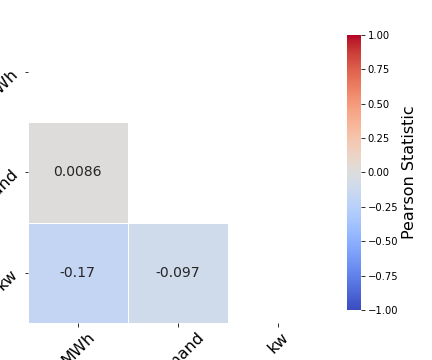
\includegraphics[width=0.8\textwidth]{solar_wind_corr.png}
  \caption{Relationships among various weather parameters and their strengths
  according to the Pearson statistic.}
  \label{fig:solar-wind-corr}
\end{figure}

Table \ref{tab:capfac} lists the average annual capacity factors for solar energy
and a hypothetical wind farm at the site of \gls{uiuc}'s Solar Farm 1.0.

\begin{table}[H]
  \centering
  \caption{Average Capacity Factors for Wind and Solar in Illinois}
  \label{tab:capfac}
  \begin{tabular}{lrr}
\toprule
Year &  Solar &   Wind \\
    &  Capacity Factor    &  Capacity Factor \\
\midrule
2010 &  0.174988 &  0.319112 \\
2011 &  0.164187 &  0.358573 \\
2012 &  0.181714 &  0.350748 \\
2013 &  0.168529 &  0.354717 \\
2014 &  0.168521 &  0.357613 \\
2015 &  0.170510 &  0.344992 \\
2016 &  0.172977 &  0.323927 \\
2017 &  0.174638 &  0.367449 \\
2018 &  0.165649 &  0.340297 \\
2019 &  0.161231 &  0.347187 \\
2020 &  0.164143 &  0.330702 \\
\bottomrule
\end{tabular}

\end{table}
